\documentclass[a4paper,oneside,english,reqno]{amsbook}
\usepackage[T1]{fontenc}
\usepackage[latin9]{inputenc}
\synctex=-1
% \usepackage{color}
\usepackage{babel}
\usepackage{textcomp}
\usepackage{mathrsfs}
\usepackage{url}
\usepackage{amstext}
\usepackage{amsthm}
\usepackage{amssymb}
\usepackage{stmaryrd}
\makeindex
\usepackage[all]{xy}

\usepackage{agt}
\hypersetup{pdftitle={Algebraic General Topology. Volume 1},
 pdfauthor={Victor Porton},
 pdfsubject={general topology},
 pdfkeywords={algebraic general topology,quasi-uniform spaces,generalizations of proximity spaces,generalizations of nearness spaces,generalizations of uniform spaces}}
% \usepackage{forwardref}
\numberwithin{section}{chapter}

% with \usepackage it fails with new TeX versions,
% without it fails with old ones. So I do neither.
% \usepackage{chngcntr}
% \counterwithout{figure}{chapter}

% Eliminate hyperref warnings: http://tex.findincity.net/view/635399273629833626247444/hyperref-token-not-allowed-warning-possible-bug
\pdfstringdefDisableCommands{%
  \let\enspace\empty  % this causes the warning for \kern
  \let\noindent\empty % this causes the warning for \indent
}

\AtEndDocument{\refstepcounter{thm}\label{finalthm}} % used in addons.tex

% \everymath{\color{blue}}

\begin{document}

\title{Algebraic General Topology. Volume 1}


\author{Victor Porton}


\email{\href{mailto:mailto:porton@narod.ru}{porton@narod.ru}}


\urladdr{\href{https://www.mathematics21.org}{https://www.mathematics21.org}}


\date{\today}


\thanks{\noun{Todd Trimble}, \noun{Andreas Blass}, \noun{Robert Martin
Solovay}, \noun{Niels Diepeveen}, and others (mentioned below) have proved some theorems which are now in this book.}
\begin{abstract}
In this work I introduce and study in details the concepts of funcoids
which generalize proximity spaces and reloids which generalize uniform
spaces, and generalizations thereof. The concept of funcoid is generalized
concept of proximity, the concept of reloid is cleared from superfluous
details (generalized) concept of uniformity. 

Also funcoids and reloids are generalizations of binary relations
whose domains and ranges are filters (instead of sets). Also funcoids
and reloids can be considered as a generalization of (oriented) graphs,
this provides us with a common generalization of calculus and discrete
mathematics.

It is defined a generalization of limit for arbitrary (including discontinuous and multivalued) functions, what allows to define for example derivative of an arbitrary real function.

The concept of continuity is defined by an algebraic formula (instead
of old messy epsilon-delta notation) for arbitrary morphisms (including
funcoids and reloids) of a partially ordered category. In one formula
continuity, proximity continuity, and uniform continuity are generalized.

Also I define connectedness for funcoids and reloids.

Then I consider generalizations of funcoids: pointfree funcoids and
generalization of pointfree funcoids: staroids and multifuncoids.
Also I define several kinds of products of funcoids and other morphisms.

Before going to topology, this book studies properties of co-brouwerian
lattices and filters.
\end{abstract}


\keywords{algebraic general topology, quasi-uniform spaces, generalizations
of proximity spaces, generalizations of nearness spaces, generalizations
of uniform spaces}


\subjclass[2010]{54J05, 54A05, 54D99, 54E05, 54E15, 54E17, 54E99}

\maketitle

\tableofcontents{}

\part{Introductory chapters}

\chapter{Introduction}

The main purpose of this book is to record the current state of my
research. The book is however written in such a way that it can be
used as a textbook for studying my research.

For the latest version of this file,
related materials, articles, research questions, and erratum consult
the Web page of the author of the book:\\
\url{http://www.mathematics21.org/algebraic-general-topology.html}


\section{License and editing}

This work is licensed under the Creative Commons Attribution 4.0 International
License. To view a copy of the license, visit\\
\href{http://creativecommons.org/licenses/by/4.0/}{http://creativecommons.org/licenses/by/4.0/}.

You can create your own copy of \LaTeX{} source of the book and edit it (to correct errors, add new results, generalize existing results,
enhance readability).
The editable source of the book is presented at\\
\href{https://bitbucket.org/portonv/algebraic-general-topology}{https://bitbucket.org/portonv/algebraic-general-topology}

Please consider reviewing this book at\\
\href{http://www.euro-math-soc.eu/node/add/book-review}{http://www.euro-math-soc.eu/node/add/book-review}

If you find any error (or some improvement idea), please report in our bug tracker:\\
\url{https://bitbucket.org/portonv/algebraic-general-topology/issues}

\section{Intended audience }

This book is suitable for any math student as well as for researchers.

To make this book be understandable even for first grade students,
I made a chapter about basic concepts (posets, lattices, topological
spaces, etc.), which an already knowledgeable person may skip reading.
It is assumed that the reader knows basic set theory.

But it is also valuable for mature researchers, as it contains much
original research which you could not find in any other source except
of my work.

Knowledge of the basic set theory is expected from the reader.

Despite that this book presents new research, it is well structured
and is suitable to be used as a textbook for a college course.

Your comments about this book are welcome to the email \href{mailto:porton@narod.ru}{porton@narod.ru}.


\section{Reading Order }

If you know basic order and lattice theory (including Galois connections
and brouwerian lattices) and basics of category theory, you may skip
reading the chapter ``\nameref{chap-common}''.

You are recommended to read the rest of this book by the order.


\section{Our topic and rationale}

From \cite{mw-gen-top}: \emph{Point-set topology, also called set-theoretic
topology or general topology, is the study of the general abstract
nature of continuity or ``closeness'' on spaces. Basic point-set
topological notions are ones like continuity, dimension, compactness,
and connectedness.}

In this work we study a new approach to point-set topology (and pointfree
topology).

Traditionally general topology is studied using topological spaces
(defined below in the section ``\nameref{sec-top}''). I however
argue that the theory of topological spaces is not the best method
of studying general topology and introduce an alternative theory,
the theory of \emph{funcoids}. Despite of popularity of the theory
of topological spaces it has some drawbacks and is in my opinion not
the most appropriate formalism to study most of general topology.
Because topological spaces are tailored for study of special sets,
so called open and closed sets, studying general topology with topological
spaces is a little anti-natural and ugly. In my opinion the theory
of funcoids is more elegant than the theory of topological spaces,
and it is better to study funcoids than topological spaces. One of
the main purposes of this work is to present an alternative General
Topology based on funcoids instead of being based on topological spaces
as it is customary. In order to study funcoids the prior knowledge
of topological spaces is not necessary. Nevertheless in this work
I will consider topological spaces and the topic of interrelation
of funcoids with topological spaces.

In fact funcoids are a generalization of topological spaces, so the
well known theory of topological spaces is a special case of the below
presented theory of funcoids.

But probably the most important reason to study funcoids is that funcoids
are a generalization of proximity spaces (see section ``\nameref{sec-prox}''
for the definition of proximity spaces). Before this work it was written
that the theory of proximity spaces was an example of a stalled research,
almost nothing interesting was discovered about this theory. It was
so because the proper way to research proximity spaces is to research
their generalization, funcoids. And so it was stalled until discovery
of funcoids. That generalized theory of proximity spaces will bring
us yet many interesting results.

In addition to \emph{funcoids} I research \emph{reloids}. Using below
defined terminology it may be said that reloids are (basically) filters
on Cartesian product of sets, and this is a special case of uniform
spaces.

Afterward we study some generalizations.

Somebody might ask, why to study it? My approach relates to traditional
general topology like complex numbers to real numbers theory. Be sure
this will find applications.

This book has a deficiency: It does not properly relate my theory
with previous research in general topology and does not consider deeper
category theory properties. It is however OK for now, as I am going
to do this study in later volumes (continuation of this book).

Many proofs in this book may seem too easy and thus this theory not
sophisticated enough. But it is largely a result of a well structured
digraph of proofs, where more difficult results are made easy by reducing
them to easier lemmas and propositions.


\section{Earlier works}

Some mathematicians were researching generalizations of proximities
and uniformities before me but they have failed to reach the right
degree of generalization which is presented in this work allowing
to represent properties of spaces with algebraic (or categorical)
formulas.

Proximity structures were introduced by Smirnov in \cite{geom-prox}.

Some references to predecessors:
\begin{itemize}
\item In \cite{gen-prox-uni1,gen-prox-uni2,some-props-prox-genunif,prox-gen-unif,compl-unif-prox}
generalized uniformities and proximities are studied.
\item Proximities and uniformities are also studied in \cite{complete-prox,prox-not-compl,compl-prox-acad,compl-prox1,compl-prox2}.
\item \cite{qunif,qunif2001} contains recent progress in quasi-uniform
spaces. \cite{qunif2001} has a very long list of related literature.
\end{itemize}
Some works (\cite{on-proximity-spaces}) about proximity spaces consider
relationships of proximities and compact topological spaces. In this
work the attempt to define or research their generalization, compactness
of funcoids or reloids is not done. It seems potentially productive
to attempt to borrow the definitions and procedures from the above
mentioned works. I hope to do this study in a separate volume.

\cite{mapping-prox} studies mappings between proximity structures.
(In this volume no attempt to research mappings between funcoids is
done.) \cite{quasi-unif-top} researches relationships of quasi-uniform
spaces and topological spaces. \cite{eq-prox-totbound-unif} studies
how proximity structures can be treated as uniform structures and
compactification regarding proximity and uniform spaces.

This book is based partially on my articles \cite{filters,funcoidsreloids,pointfree}.


\section{Kinds of continuity}

A research result based on this book but not fully included in this
book (and not yet published) is that the following kinds of continuity
are described by the same algebraic (or rather categorical) formulas
for different kinds of continuity and have common properties:
\begin{itemize}
\item discrete continuity (between digraphs);
\item (pre)topological continuity;
\item proximal continuity;
\item uniform continuity;
\item Cauchy continuity;
\item (probably other kinds of continuity).
\end{itemize}
Thus my research justifies using the same word ``continuity'' for
these diverse kinds of continuity.

See \url{http://www.mathematics21.org/algebraic-general-topology.html}

\section{Responses to some accusations against style of my exposition}

\begin{quote}
The proofs are generally hard to follow and unpleasant to read as they are just a bunch of equations thrown at you, without motivation or underlying reasoning, etc.
\end{quote}

I don't think this is essential. The proofs are not the most important thing in my book. The most essential thing are definitions. The proofs are just to fill the gaps. So I deem it not important whether proofs are motivated.

Also, note ``algebraic'' in the title of my book. The proofs are meant to be just sequences of formulas for as much as possible :-) It is to be thought algebraically. The meaning are the formulas themselves.

Maybe it makes sense to read my book skipping all the proofs? Some proofs contain important ideas, but most don't. The important thing are definitions.

\section{Structure of this book}

In the chapter ``\nameref{chap-common}'' some well known definitions
and theories are considered. You may skip its reading if you already
know it. That chapter contains info about:
\begin{itemize}
\item posets;
\item lattices and complete lattices;
\item Galois connections;
\item co-brouwerian lattices;
\item a very short intro into category theory;
\item a very short introduction to group theory.
\end{itemize}
Afterward there are my little additions to poset/lattice and category
theory.

Afterward there is the theory of filters and filtrators.

Then there is ``\nameref{common-top}'', which considers briefly:
\begin{itemize}
\item metric spaces;
\item topological spaces;
\item pretopological spaces;
\item proximity spaces.
\end{itemize}
Despite of the name ``Common knowledge'' this second common knowledge
chapter is recommended to be read completely even if you know topology
well, because it contains some rare theorems not known to most mathematicians
and hard to find in literature.

Then the most interesting thing in this book, the theory of funcoids,
starts.

Afterwards there is the theory of reloids.

Then I show relationships between funcoids and reloids.

The last I research generalizations of funcoids, \emph{pointfree funcoids},
\emph{staroids}, and \emph{multifuncoids} and some different kinds
of products of morphisms.


\section{Basic notation}

I will denote a set definition like $\setcond{x\in A}{P(x)}$ instead
of customary $\{x\in A\mid P(x)\}$. I do this because otherwise formulas
don't fit horizontally into the available space.


\subsection{\index{Grothendieck universe}Grothendieck universes}

We will work in ZFC with an infinite and uncountable Grothendieck
universe.

A Grothendieck universe is just a set big enough to make all usual
set theory inside it. For example if $\mho$ is a Grothendieck universe,
and sets $X,Y\in\mho$, then also $X\cup Y\in\mho$, $X\cap Y\in\mho$,
$X\times Y\in\mho$, etc.

\index{small set}A set which is a member of a Grothendieck universe
is called a \emph{small set} (regarding this Grothendieck universe).
We can restrict our consideration to small sets in order to get rid
troubles with proper classes.
\begin{defn}
Grothendieck universe is a set $\mho$ such that:
\begin{enumerate}
\item If $x\in\mho$ and $y\in x$ then $y\in\mho$.
\item If $x,y\in\mho$ then $\{x,y\}\in\mho$.
\item If $x\in\mho$ then $\subsets x\in\mho$.
\item If $\setcond{x_{i}}{i\in I\in\mho}$ is a family of elements of $\mho$,
then $\bigcup_{i\in I}x_{i}\in\mho$.
\end{enumerate}
\end{defn}
One can deduce from this also:
\begin{enumerate}
\item If $x\in\mho$, then $\{x\}\in\mho$.
\item If $x$ is a subset of $y\in\mho$, then $x\in\mho$.
\item If $x,y\in\mho$ then the ordered pair $(x,y)=\{\{x,y\},x\}\in\mho$.
\item If $x,y\in\mho$ then $x\cup y$ and $x\times y$ are in $\mho$.
\item If $\setcond{x_{i}}{i\in I\in\mho}$ is a family of elements of $\mho$,
then the product $\prod_{i\in I}x_{i}\in\mho$.
\item If $x\in\mho$, then the cardinality of $x$ is strictly less than
the cardinality of~$\mho$.
\end{enumerate}

\subsection{Misc}

In this book quantifiers bind tightly. That is $\forall x\in A:P(x)\land Q$
and $\forall x\in A:P(x)\Rightarrow Q$ should be read $\left(\forall x\in A:P(x)\right)\land Q$
and $\left(\forall x\in A:P(x)\right)\Rightarrow Q$ not $\forall x\in A:\left(P(x)\land Q\right)$
and $\forall x\in A:\left(P(x)\Rightarrow Q\right)$.

The set of functions from a set $A$ to a set $B$ is denoted as $B^{A}$.

I will often skip parentheses and write $fx$ instead of $f(x)$ to
denote the result of a function $f$ acting on the argument $x$.

I will denote $\rsupfun fX=\setcond{\beta\in\im f}{\exists\alpha\in X:\alpha\mathrel f\beta}$
(in other words $\rsupfun fX$ is the image of a set~$X$ under a function or binary relation~$f$)
and $X\rsuprel fY\Leftrightarrow\exists x\in X,y\in Y:x\mathrel{f}y$
for sets $X$, $Y$ and a binary relation $f$. (Note that functions
are a special case of binary relations.)

By just $\rsupfun f$ and $\rsuprel f$ I will denote the corresponding
function and relation on small sets.

\begin{obvious}
For a function~$f$ we have $\rsupfun{f}X = \setcond{f(x)}{x\in X}$.
\end{obvious}

\begin{defn}
$\rsupfun{f^{-1}}X$ is called the \emph{preimage} of a set~$X$ by a function (or, more generally, a binary relation)~$f$.
\end{defn}

\begin{obvious}
$\{\alpha\}\rsuprel f\{\beta\}\Leftrightarrow\alpha\mathrel f\beta$
for every $\alpha$ and $\beta$.
\end{obvious}
$\mylambda xD{f(x)}=\setcond{(x,f(x))}{x\in D}$ for a set $D$ and
and a form $f$ depending on the variable $x$.
In other words, $\mylambda xD{f(x)}$ is the function which maps elements~$x$ of a set~$D$ into $f(x)$.

I will denote source and destination of a morphism $f$ of any category
(See chapter~\ref{chap-common} for a definition of a category.)
as $\Src f$ and $\Dst f$ correspondingly. Note that below defined
domain and image of a funcoid are not the same as its source and destination.

I will denote $\GR(A,B,f)=f$ for any morphism $(A,B,f)$ of either
$\mathbf{Set}$ or $\mathbf{Rel}$. (See definitions of $\mathbf{Set}$
and $\mathbf{Rel}$ below.)

\section{Implicit arguments}

Some notation such that $\bot^{\mathfrak{A}}$, $\top^{\mathfrak{A}}$,
$\sqcup^{\mathfrak{A}}$, $\sqcap^{\mathfrak{A}}$ have indexes (in these examples~$\mathfrak{A}$).

We will omit these indexes when they can be restored from the context. For example,
having a function $f:\mathfrak{A}\rightarrow\mathfrak{B}$ where $\mathfrak{A}$,~$\mathfrak{B}$
are posets with least elements, we will concisely denote $f\bot = \bot$ for $f\bot^{\mathfrak{A}} = \bot^{\mathfrak{B}}$.
(See below for definitions of these operations.)

\begin{note}
In the above formula $f\bot = \bot$ we have the first~$\bot$ and the second~$\bot$ denoting different objects.
\end{note}

We will assume (skipping this in actual proofs) that all omitted indexes can be restored from context.
(Note that so called dependent type theory computer proof assistants do this like we implicitly.)
\section{Unusual notation}

In the chapter ``\nameref{chap-common}'' (which you may skip reading
if you are already knowledgeable) some non-standard notation is defined.
I summarize here this notation for the case if you choose to skip
reading that chapter:

Partial order is denoted as $\sqsubseteq$.

Meets and joins are denoted as $\sqcap$, $\sqcup$, $\bigsqcap$,
$\bigsqcup$.

I call element $b$ \emph{substractive} from an element~$a$ (of a distributive
lattice $\mathfrak{A}$) when the difference $a\setminus b$ exists.
I call $b$ \emph{complementive} to $a$ when there exists $c\in\mathfrak{A}$
such that $b\sqcap c=\bot$ and $b\sqcup c=a$. We will prove that
$b$ is complementive to $a$ iff $b$ is substractive from $a$ and
$b\sqsubseteq a$.
\begin{defn}
Call $a$ and $b$ of a poset $\mathfrak{A}$ \emph{intersecting},
denoted $a\nasymp b$, when there exists a non-least element $c$
such that $c\sqsubseteq a\land c\sqsubseteq b$.
\end{defn}

\begin{defn}
$a\asymp b\eqdef\lnot(a\nasymp b)$.
\end{defn}

\begin{defn}
I call elements $a$ and $b$ of a poset $\mathfrak{A}$ \emph{joining}
and denote $a\equiv b$ when there are no non-greatest element $c$
such that $c\sqsupseteq a\land c\sqsupseteq b$.
\end{defn}

\begin{defn}
$a\nequiv b\eqdef\lnot(a\equiv b)$.\end{defn}
\begin{obvious}
$a\nasymp b$ iff $a\sqcap b$ is non-least, for every elements $a$,
$b$ of a meet-semilattice.
\end{obvious}

\begin{obvious}
$a\equiv b$ iff $a\sqcup b$ is the greatest element, for every elements
$a$, $b$ of a join-semilattice.
\end{obvious}
I extend the definitions of pseudocomplement and dual pseudocomplement
to arbitrary posets (not just lattices as it is customary):
\begin{defn}
Let $\mathfrak{A}$ be a poset. \emph{Pseudocomplement} of $a$ is
\[
\max\setcond{c\in\mathfrak{A}}{c\asymp a}.
\]


If $z$ is the pseudocomplement of $a$ we will denote $z=a^{\ast}$.
\end{defn}

\begin{defn}
Let $\mathfrak{A}$ be a poset. \emph{Dual pseudocomplement} of $a$
is
\[
\min\setcond{c\in\mathfrak{A}}{c\equiv a}.
\]


If $z$ is the dual pseudocomplement of $a$ we will denote $z=a^{+}$.\end{defn}


% 
\chapter{\label{chap-common}Common knowledge, part 1}

In this chapter we will consider some well known mathematical theories.
If you already know them you may skip reading this chapter (or its
parts).


\section{Order theory}


\subsection{Posets}
\begin{defn}
\index{identity relation}The \emph{identity relation} on a set $A$
is $\id_{A}=\setcond{(a,a)}{a\in A}$.
\end{defn}

\begin{defn}
\index{preorder}A \emph{preorder} on a set $A$ is a binary relation~$\sqsubseteq$ on~$A$ which is:
\begin{itemize}
\item \emph{reflexive} on $A$ that is $\opinparens{\sqsubseteq}\supseteq\id_{A}$ or what is the same $\forall x\in A:x\sqsubseteq x$;
\item \emph{transitive} that is $\opinparens{\sqsubseteq}\circ\opinparens{\sqsubseteq}\subseteq\opinparens{\sqsubseteq}$
 or what is the same \[ \forall x,y,z:(x\sqsubseteq y\land y\sqsubseteq z\Rightarrow x\sqsubseteq z). \]
\end{itemize}
\end{defn}

\begin{defn}
\index{partial order}A \emph{partial order} on a set $A$ is a preorder
on $A$ which is \emph{antisymmetric} that is $\opinparens{\sqsubseteq}\cap\opinparens{\sqsubseteq}\subseteq\id_A$
or what is the same \[ \forall x,y\in A:(x\sqsubseteq y\land y\sqsubseteq x\Rightarrow x=y). \]
\end{defn}
The reverse relation is denoted $\sqsupseteq$.

\begin{defn}
\index{subelement}$a$ is a subelement of $b$ (or what is the same
$a$ is \emph{contained} in $b$ or $b$ \emph{contains} $a$) iff
$a\sqsubseteq b$.\end{defn}
\begin{obvious}
The reverse of a partial order is also a partial order.\end{obvious}
\begin{defn}
\index{set!partially ordered}\index{poset}A set $A$ together with
a partial order on it is called a \emph{partially ordered set} (\emph{poset}
for short).
\end{defn}

An example of a poset is the set~$\mathbb{R}$ of real numbers with $\mathord{\sqsubseteq} = \mathord{\leq}$.

Another example is the set~$\subsets A$ of all subsets of an arbitrary fixed set~$A$ with $\mathord{\sqsubseteq} = \mathord{\subseteq}$.
Note that this poset is (in general) not linear (see definition of \emph{linear} poset below.)

\begin{defn}
\index{partial order!strict}Strict partial order $\sqsubset$ corresponding
to the partial order $\sqsubseteq$ on a set $A$ is defined by the
formula $\opinparens{\sqsubset}=\opinparens{\sqsubseteq}\setminus\id_{A}$.
In other words, \[ a\sqsubset b\Leftrightarrow a\sqsubseteq b\land a\ne b. \]
\end{defn}

An example of strict partial order is~$<$ on the set~$\mathbb{R}$ of real numbers.

\begin{defn}
\index{partial order!restricted}A partial order on a set $A$ \emph{restricted}
to a set $B\subseteq A$ is $\opinparens{\sqsubseteq}\cap(B\times B)$.\end{defn}
\begin{obvious}
A partial order on a set $A$ restricted to a set $B\subseteq A$
is a partial order on $B$.\end{obvious}
\begin{defn}
~
\begin{itemize}
\item \index{least element}The \emph{least} element $\bot$ of a poset
$\mathfrak{A}$ is defined by the formula $\forall a\in\mathfrak{A}:\bot\sqsubseteq a$.
\item \index{greatest element}The \emph{greatest} element $\top$ of a
poset $\mathfrak{A}$ is defined by the formula $\forall a\in\mathfrak{A}:\top\sqsupseteq a$.
\end{itemize}
\end{defn}
\begin{prop}
There exist no more than one least element and no more than one greatest
element (for a given poset).\end{prop}
\begin{proof}
By antisymmetry.\end{proof}
\begin{defn}
\index{dual!order}The \emph{dual} order for $\sqsubseteq$ is $\sqsupseteq$.\end{defn}
\begin{obvious}
Dual of a partial order is a partial order.\end{obvious}
\begin{defn}
\index{dual!poset}The \emph{dual} poset for a poset $(A,\mathord{\sqsubseteq})$
is the poset $(A,\mathord{\sqsupseteq})$.
\end{defn}
I will denote dual of a poset~$\mathfrak{A}$ as $(\dual\mathfrak{A})$
and dual of an element~$a\in\mathfrak{A}$ (that is the same element
in the dual poset) as $(\dual a)$.

\index{duality!partial order}Below we will sometimes use \emph{duality}
that is replacement of the partial order and all related operations
and relations with their duals. In other words, it is enough to prove
a theorem for an order $\sqsubseteq$ and the similar theorem for
$\sqsupseteq$ follows by duality.

\begin{defn}
\index{bounded above}
\index{bounded below}
A subset~$P$ of a poset~$\mathfrak{A}$ is called \emph{bounded
above} if there exists $t\in\mathfrak{A}$ such that
$\forall x\in P:t\sqsupseteq x$. \emph{Bounded below} is
defined dually.
\end{defn}

\subsubsection{Intersecting and joining elements}

Let $\mathfrak{A}$ be a poset.
\begin{defn}
\index{intersecting elements}Call elements $a$ and $b$ of $\mathfrak{A}$
\emph{intersecting}, denoted $a\nasymp b$, when there exists a non-least
element $c$ such that $c\sqsubseteq a\land c\sqsubseteq b$.
\end{defn}

\begin{defn}
$a\asymp b\eqdef\lnot(a\nasymp b)$.\end{defn}
\begin{obvious}
$a_{0}\nasymp b_{0}\land a_{1}\sqsupseteq a_{0}\land b_{1}\sqsupseteq b_{0}\Rightarrow a_{1}\nasymp b_{1}$.\end{obvious}
\begin{defn}
\index{joining elements}I call elements $a$ and $b$ of $\mathfrak{A}$
\emph{joining} and denote $a\equiv b$ when there is no a non-greatest
element $c$ such that $c\sqsupseteq a\land c\sqsupseteq b$.
\end{defn}

\begin{defn}
$a\nequiv b\eqdef\lnot(a\equiv b)$.\end{defn}
\begin{obvious}
Intersecting is the dual of non-joining.
\end{obvious}

\begin{obvious}
$a_{0}\equiv b_{0}\land a_{1}\sqsupseteq a_{0}\land b_{1}\sqsupseteq b_{0}\Rightarrow a_{1}\equiv b_{1}$.
\end{obvious}

\subsection{Linear order}
\begin{defn}
\index{linearly ordered set}A poset $\mathfrak{A}$ is called \emph{linearly
ordered set} (or what is the same, \emph{totally ordered set}) if
$a\sqsupseteq b\lor b\sqsupseteq a$ for every $a,b\in\mathfrak{A}$.\end{defn}
\begin{example}
The set of real numbers with the customary order is a linearly ordered
set.\end{example}
\begin{defn}
\index{chain}A set $X\in\subsets\mathfrak{A}$ where $\mathfrak{A}$
is a poset is called \emph{chain} if $\mathfrak{A}$ restricted to
$X$ is a total order.
\end{defn}

\subsection{Meets and joins}

Let $\mathfrak{A}$ be a poset.
\begin{defn}
\index{least element}Given a set $X\in\subsets\mathfrak{A}$ the
\emph{least element} (also called \emph{minimum} and denoted $\min X$)
of $X$ is such $a\in X$ that $\forall x\in X:a\sqsubseteq x$.
\end{defn}
Least element does not necessarily exists. But if it exists:
\begin{prop}
For a given $X\in\subsets\mathfrak{A}$ there exist no more than one
least element.\end{prop}
\begin{proof}
It follows from anti-symmetry.
\end{proof}
\emph{Greatest element} is the dual of least element:
\begin{defn}
\index{greatest element}Given a set $X\in\subsets\mathfrak{A}$ the
\emph{greatest element} (also called \emph{maximum} and denoted $\max X$)
of $X$ is such $a\in X$ that $\forall x\in X:a\sqsupseteq x$.\end{defn}
\begin{rem}
Least and greatest elements of a set $X$ is a trivial generalization
of the above defined least and greatest element for the entire poset.\end{rem}
\begin{defn}
~
\begin{itemize}
\item \index{minimal element}A \emph{minimal} element of a set $X\in\subsets\mathfrak{A}$
is such $a\in\mathfrak{A}$ that $\nexists x\in X:a\sqsupset x$.
\item \index{maximal element}A \emph{maximal} element of a set $X\in\subsets\mathfrak{A}$
is such $a\in\mathfrak{A}$ that $\nexists x\in X:a\sqsubset x$.
\end{itemize}
\end{defn}
\begin{rem}
Minimal element is not the same as minimum, and maximal element is
not the same as maximum.\end{rem}
\begin{obvious}
~
\begin{enumerate}
\item The least element (if it exists) is a minimal element.
\item The greatest element (if it exists) is a maximal element.
\end{enumerate}
\end{obvious}
\begin{xca}
Show that there may be more than one minimal and more than one maximal
element for some poset.\end{xca}
\begin{defn}
\index{bounds!upper}\emph{Upper bounds} of a set $X$ is the set
$\setcond{y\in\mathfrak{A}}{\forall x\in X:y\sqsupseteq x}$.
\end{defn}
The dual notion:
\begin{defn}
\index{bounds!lower}\emph{Lower bounds} of a set $X$ is the set
$\setcond{y\in\mathfrak{A}}{\forall x\in X:y\sqsubseteq x}$.
\end{defn}

\begin{defn}
\index{join}\index{supremum}\emph{Join} $\bigsqcup X$ (also called
\emph{supremum} and denoted ``$\sup X$'') of a set $X$ is the
least element of its upper bounds (if it exists).
\end{defn}

\begin{defn}
\index{meet}\index{infimum}\emph{Meet} $\bigsqcap X$ (also called
\emph{infimum} and denoted ``$\inf X$'') of a set $X$ is the greatest
element of its lower bounds (if it exists).
\end{defn}
We will also denote $\bigsqcup_{i\in X}f(i)=\bigsqcup\setcond{f(i)}{x\in X}$
and $\bigsqcap_{i\in X}f(i)=\bigsqcap\setcond{f(i)}{x\in X}$.

We will write $b=\bigsqcup X$ when $b\in\mathfrak{A}$ is the join
of $X$ or say that $\bigsqcup X$ does not exist if there are no
such $b\in\mathfrak{A}$. (And dually for meets.)
\begin{xca}
Provide an example of $\bigsqcup X\notin X$ for some set $X$ on
some poset.\end{xca}
\begin{prop}
~
\begin{enumerate}
\item If $b$ is the greatest element of $X$ then $\bigsqcup X=b$.
\item If $b$ is the least element of $X$ then $\bigsqcap X=b$.
\end{enumerate}
\end{prop}
\begin{proof}
We will prove only the first as the second is dual.

Let $b$ be the greatest element of $X$. Then upper bounds of $X$
are $\setcond{y\in\mathfrak{A}}{y\sqsupseteq b}$. Obviously $b$
is the least element of this set, that is the join.\end{proof}
\begin{defn}
\index{join!binary}\emph{Binary joins and meets} are defined by the
formulas
\[
x\sqcup y=\bigsqcup\{x,y\}\quad\text{and}\quad x\sqcup y=\bigsqcap\{x,y\}.
\]
\end{defn}
\begin{obvious}
$\sqcup$ and $\sqcap$ are symmetric operations (whenever these are
defined for given $x$ and $y$).\end{obvious}
\begin{thm}
~
\begin{enumerate}
\item If $\bigsqcup X$ exists then $y\sqsupseteq\bigsqcup X\Leftrightarrow\forall x\in X:y\sqsupseteq x$.
\item If $\bigsqcap X$ exists then $y\sqsubseteq\bigsqcap X\Leftrightarrow\forall x\in X:y\sqsubseteq x$.
\end{enumerate}
\end{thm}
\begin{proof}
I will prove only the first as the second follows by duality.

$y\sqsupseteq\bigsqcup X\Leftrightarrow y\text{ is an upper bound for }X\Leftrightarrow\forall x\in X:y\sqsupseteq x$.
\end{proof}
\begin{cor}
~
\begin{enumerate}
\item If $a\sqcup b$ exists then $y\sqsupseteq a\sqcup b\Leftrightarrow y\sqsupseteq a\land y\sqsupseteq b$.
\item If $a\sqcap b$ exists then $y\sqsubseteq a\sqcap b\Leftrightarrow y\sqsubseteq a\land y\sqsubseteq b$.
\end{enumerate}
\end{cor}
I will denote meets and joins for a specific poset $\mathfrak{A}$
as $\bigsqcap^{\mathfrak{A}}$, $\bigsqcup^{\mathfrak{A}}$, $\sqcap^{\mathfrak{A}}$,
$\sqcup^{\mathfrak{A}}$.


\subsection{Semilattices}
\begin{defn}
~
\begin{enumerate}
\item \index{semilattice!join-semilattice}A \emph{join-semilattice} is
a poset $\mathfrak{A}$ such that $a\sqcup b$ is defined for every
$a,b\in\mathfrak{A}$.
\item \index{semilattice!meet-semilattice}A \emph{meet-semilattice} is
a poset $\mathfrak{A}$ such that $a\sqcap b$ is defined for every
$a,b\in\mathfrak{A}$.
\end{enumerate}
\end{defn}
\begin{thm}
~
\begin{enumerate}
\item The operation $\sqcup$ is associative for any join-semilattice.
\item The operation $\sqcap$ is associative for any meet-semilattice.
\end{enumerate}
\end{thm}
\begin{proof}
I will prove only the first as the second follows by duality.

We need to prove $(a\sqcup b)\sqcup c=a\sqcup(b\sqcup c)$ for every
$a,b,c\in\mathfrak{A}$.

Taking into account the definition of join, it is enough to prove
that
\[
x\sqsupseteq(a\sqcup b)\sqcup c\Leftrightarrow x\sqsupseteq a\sqcup(b\sqcup c)
\]
for every $x\in\mathfrak{A}$. Really, this follows from the chain
of equivalences:
\begin{align*}
x\sqsupseteq(a\sqcup b)\sqcup c & \Leftrightarrow\\
x\sqsupseteq a\sqcup b\land x\sqsupseteq c & \Leftrightarrow\\
x\sqsupseteq a\land x\sqsupseteq b\land x\sqsupseteq c & \Leftrightarrow\\
x\sqsupseteq a\land x\sqsupseteq b\sqcup c & \Leftrightarrow\\
x\sqsupseteq a\sqcup(b\sqcup c).
\end{align*}
\end{proof}
\begin{obvious}
$a\nasymp b$ iff $a\sqcap b$ is non-least, for every elements $a$,
$b$ of a meet-semilattice.
\end{obvious}

\begin{obvious}
$a\equiv b$ iff $a\sqcup b$ is the greatest element, for every elements
$a$, $b$ of a join-semilattice.
\end{obvious}

\subsection{Lattices and complete lattices}
\begin{defn}
\index{poset!bounded}A \emph{bounded} poset is a poset having both
least and greatest elements.
\end{defn}

\begin{defn}
\index{lattice}\emph{Lattice} is a poset which is both join-semilattice
and meet-semilattice.
\end{defn}

\begin{defn}
\index{lattice!complete}A \emph{complete lattice} is a poset $\mathfrak{A}$
such that for every $X\in\subsets\mathfrak{A}$ both $\bigsqcup X$
and $\bigsqcap X$ exist.\end{defn}
\begin{obvious}
Every complete lattice is a lattice.\end{obvious}
\begin{prop}
Every complete lattice is a bounded poset.\end{prop}
\begin{proof}
$\bigsqcup\emptyset$ is the least and $\bigsqcap\emptyset$ is the
greatest element.\end{proof}
\begin{thm}
Let $\mathfrak{A}$ be a poset.
\begin{enumerate}
\item If $\bigsqcup X$ is defined for every $X\in\subsets\mathfrak{A}$,
then $\mathfrak{A}$ is a complete lattice.
\item If $\bigsqcap X$ is defined for every $X\in\subsets\mathfrak{A}$,
then $\mathfrak{A}$ is a complete lattice.
\end{enumerate}
\end{thm}
\begin{proof}
See \cite{pm:complete-lattice-criteria} or any lattice theory reference.\end{proof}
\begin{obvious}
If $X\subseteq Y$ for some $X,Y\in\subsets\mathfrak{A}$ where $\mathfrak{A}$
is a complete lattice, then
\begin{enumerate}
\item $\bigsqcup X\sqsubseteq\bigsqcup Y$;
\item $\bigsqcap X\sqsupseteq\bigsqcap Y$.
\end{enumerate}
\end{obvious}
\begin{prop}
If $S\in\subsets\subsets\mathfrak{A}$ then for every complete lattice
$\mathfrak{A}$
\begin{enumerate}
\item $\bigsqcup\bigcup S=\bigsqcup_{X\in S}\bigsqcup X$;
\item $\bigsqcap\bigcup S=\bigsqcap_{X\in S}\bigsqcap X$.
\end{enumerate}
\end{prop}
\begin{proof}
We will prove only the first as the second is dual.

By definition of joins, it is enough to prove $y\sqsupseteq\bigsqcup\bigcup S\Leftrightarrow y\sqsupseteq\bigsqcup_{X\in S}\bigsqcup X$.

Really,
\begin{align*}
y\sqsupseteq\bigsqcup\bigcup S & \Leftrightarrow\\
\forall x\in\bigcup S:y\sqsupseteq x & \Leftrightarrow\\
\forall X\in S\forall x\in X:y\sqsupseteq x & \Leftrightarrow\\
\forall X\in S:y\sqsupseteq\bigsqcup X & \Leftrightarrow\\
y\sqsupseteq\bigsqcup_{X\in S}\bigsqcup X.
\end{align*}
\end{proof}
\begin{defn}
A \emph{sublattice} of a lattice is it subset closed regarding~$\sqcup$
and~$\sqcap$.\end{defn}
\begin{obvious}
Sublattice with induced order is also a lattice.
\end{obvious}

\subsection{Distributivity of lattices}
\begin{defn}
\index{lattice!distributive}A \emph{distributive} lattice is such
lattice $\mathfrak{A}$ that for every $x,y,z\in\mathfrak{A}$
\begin{enumerate}
\item $x\sqcap(y\sqcup z)=(x\sqcap y)\sqcup(x\sqcap z)$;
\item $x\sqcup(y\sqcap z)=(x\sqcup y)\sqcap(x\sqcup z)$.
\end{enumerate}
\end{defn}
\begin{thm}
For a lattice to be distributive it is enough just one of the conditions:
\begin{enumerate}
\item $x\sqcap(y\sqcup z)=(x\sqcap y)\sqcup(x\sqcap z)$;
\item $x\sqcup(y\sqcap z)=(x\sqcup y)\sqcap(x\sqcup z)$.
\end{enumerate}
\end{thm}
\begin{proof}
~

\begin{align*}
(x\sqcup y)\sqcap(x\sqcup z) & =\\
((x\sqcup y)\sqcap x)\sqcup((x\sqcup y)\sqcap z) & =\\
x\sqcup((x\sqcap z)\sqcup(y\sqcap z)) & =\\
(x\sqcup(x\sqcap z))\sqcup(y\sqcap z) & =\\
x\sqcup(y\sqcap z)
\end{align*}


(applied $x\sqcap(y\sqcup z)=(x\sqcap y)\sqcup(x\sqcap z)$ twice).
\end{proof}

\subsection{Difference and complement}
\begin{defn}
\index{difference}\index{substractive}Let $\mathfrak{A}$ be a distributive
lattice with least element $\bot$. The \emph{difference} (denoted
$a\setminus b$) of elements $a$ and $b$ is such $c\in\mathfrak{A}$
that $b\sqcap c=\bot$ and $a\sqcup b=b\sqcup c$. I will call $b$
\emph{substractive} from \textbf{$a$} when $a\setminus b$ exists.\end{defn}
\begin{thm}
If $\mathfrak{A}$ is a distributive lattice with least element $\bot$,
there exists no more than one difference of elements $a$, $b$.\end{thm}
\begin{proof}
Let $c$ and $d$ be both differences $a\setminus b$. Then $b\sqcap c=b\sqcap d=\bot$
and $a\sqcup b=b\sqcup c=b\sqcup d$. So
\[
c=c\sqcap(b\sqcup c)=c\sqcap(b\sqcup d)=(c\sqcap b)\sqcup(c\sqcap d)=\bot\sqcup(c\sqcap d)=c\sqcap d.
\]


Similarly $d=d\sqcap c$. Consequently $c=c\sqcap d=d\sqcap c=d$.\end{proof}
\begin{defn}
\index{complementive}I will call $b$ \emph{complementive} to $a$
iff there exists $c\in\mathfrak{A}$ such that $b\sqcap c=\bot$ and
$b\sqcup c=a$.\end{defn}
\begin{prop}
$b$ is complementive to $a$ iff $b$ is substractive from $a$ and
$b\sqsubseteq a$.\end{prop}
\begin{proof}
~
\begin{description}
\item [{$\Leftarrow$}] Obvious.
\item [{$\Rightarrow$}] We deduce $b\sqsubseteq a$ from $b\sqcup c=a$.
Thus $a\sqcup b=a=b\sqcup c$.
\end{description}
\end{proof}
\begin{prop}
If $b$ is complementive to $a$ then $(a\setminus b)\sqcup b=a$.\end{prop}
\begin{proof}
Because $b\sqsubseteq a$ by the previous proposition.\end{proof}
\begin{defn}
\index{complement}Let $\mathfrak{A}$ be a bounded distributive lattice.
The \emph{complement} (denoted $\bar{a}$) of an element $a\in\mathfrak{A}$
is such $b\in\mathfrak{A}$ that $a\sqcap b=\bot$ and $a\sqcup b=\top$.\end{defn}
\begin{prop}
If $\mathfrak{A}$ is a bounded distributive lattice then $\bar{a}=\top\setminus a$.\end{prop}
\begin{proof}
$b=\bar{a}\Leftrightarrow b\sqcap a=\bot\land b\sqcup a=\top\Leftrightarrow b\sqcap a=\bot\land\top\sqcup a=a\sqcup b\Leftrightarrow b=\top\setminus a$.\end{proof}
\begin{cor}
If $\mathfrak{A}$ is a bounded distributive lattice then exists no
more than one complement of an element $a\in\mathfrak{A}$.\end{cor}
\begin{defn}
\index{complemented!element}An element of bounded distributive lattice
is called \emph{complemented} when its complement exists.
\end{defn}

\begin{defn}
\index{complemented!lattice}A distributive lattice is a \emph{complemented
lattice} iff every its element is complemented.\end{defn}
\begin{prop}
For a distributive lattice $(a\setminus b)\setminus c=a\setminus(b\sqcup c)$
if $a\setminus b$ and $(a\setminus b)\setminus c$ are defined.\end{prop}
\begin{proof}
$((a\setminus b)\setminus c)\sqcap c=\bot$; $((a\setminus b)\setminus c)\sqcup c=(a\setminus b)\sqcup c$;
$(a\setminus b)\sqcap b=\bot$; $(a\setminus b)\sqcup b=a\sqcup b$.

We need to prove $((a\setminus b)\setminus c)\sqcap(b\sqcup c)=\bot$
and $((a\setminus b)\setminus c)\sqcup(b\sqcup c)=a\sqcup(b\sqcup c)$.

In fact,
\begin{align*}
((a\setminus b)\setminus c)\sqcap(b\sqcup c) & =\\
(((a\setminus b)\setminus c)\sqcap b)\sqcup(((a\setminus b)\setminus c)\sqcap c) & =\\
(((a\setminus b)\setminus c)\sqcap b)\sqcup\bot & =\\
((a\setminus b)\setminus c)\sqcap b & \sqsubseteq\\
(a\setminus b)\sqcap b & =\bot,
\end{align*}


so $((a\setminus b)\setminus c)\sqcap(b\sqcup c)=\bot$;
\begin{align*}
((a\setminus b)\setminus c)\sqcup(b\sqcup c) & =\\
(((a\setminus b)\setminus c)\sqcup c)\sqcup b & =\\
(a\setminus b)\sqcup c\sqcup b & =\\
((a\setminus b)\sqcup b)\sqcup c & =\\
a\sqcup b\sqcup c.
\end{align*}

\end{proof}

\subsection{Boolean lattices}
\begin{defn}
\index{lattice!boolean}A \emph{boolean lattice} is a complemented
distributive lattice.
\end{defn}
The most important example of a boolean lattice is $\subsets A$ where
\textbf{$A$} is a set, ordered by set inclusion.
\begin{thm}
\index{Morgan's laws}(\noun{De Morgan}'s laws) For every elements $a$,
$b$ of a boolean lattice
\begin{enumerate}
\item $\overline{a\sqcup b}=\bar{a}\sqcap\bar{b}$;
\item $\overline{a\sqcap b}=\bar{a}\sqcup b$.
\end{enumerate}
\end{thm}
\begin{proof}
We will prove only the first as the second is dual.

It is enough to prove that $a\sqcup b$ is a complement of $\bar{a}\sqcap\bar{b}$.
Really:
\begin{gather*}
(a\sqcup b)\sqcap(\bar{a}\sqcap\bar{b})\sqsubseteq a\sqcap(\bar{a}\sqcap\bar{b})=(a\sqcap\bar{a})\sqcap\bar{b}=\bot\sqcap\bar{b}=\bot;\\
(a\sqcup b)\sqcup(\bar{a}\sqcap\bar{b})=((a\sqcup b)\sqcup\bar{a})\sqcap((a\sqcup b)\sqcup\bar{b})\sqsupseteq(a\sqcup\bar{a})\sqcap(b\sqcup\bar{b})=\top\sqcap\top=\top.
\end{gather*}


Thus $(a\sqcup b)\sqcap(\bar{a}\sqcap\bar{b})=\bot$ and $(a\sqcup b)\sqcup(\bar{a}\sqcap\bar{b})=\top$.\end{proof}
\begin{defn}
\index{join infinite distributive}A complete lattice $\mathfrak{A}$
is \emph{join infinite distributive} when $x\sqcap\bigsqcup S=\bigsqcup\rsupfun{x\sqcap}S$;
\index{meet infinite distributive}a complete lattice $\mathfrak{A}$
is \emph{meet infinite distributive} when $x\sqcup\bigsqcap S=\bigsqcap\rsupfun{x\sqcup}S$
for all $x\in\mathfrak{A}$ and $S\in\subsets\mathfrak{A}$.
\end{defn}

\begin{defn}
\index{infinite distributive}\emph{Infinite distributive complete
lattice} is a complete lattice which is both join infinite distributive
and meet infinite distributive.\end{defn}

\begin{thm}\label{bool-inf-distr1}
For every boolean lattice~$\mathfrak{A}$, $x\in\mathfrak{A}$ and $S\in\subsets\mathfrak{A}$ we have:
\begin{enumerate}
\item $\bigsqcup\rsupfun{x\sqcap}S$ is defined and $x\sqcap\bigsqcup S=\bigsqcup\rsupfun{x\sqcap}S$ whenever $\bigsqcup S$ is defined.
\item $\bigsqcap\rsupfun{x\sqcup}S$ is defined and $x\sqcup\bigsqcap S=\bigsqcap\rsupfun{x\sqcup}S$ whenever $\bigsqcap S$ is defined.
\end{enumerate}
\end{thm}

\begin{proof}
We will prove only the first, as the other is dual.

We need to prove that $x\sqcap\bigsqcup S$ is the least upper bound of $\rsupfun{x\sqcap}S$.

That $x\sqcap\bigsqcup S$ is an upper bound of $\rsupfun{x\sqcap}S$ is obvious.

Now let \textbf{$u$} be any upper bound of $\rsupfun{x\sqcap}S$,
that is $x\sqcap y\sqsubseteq u$ for all $y\in S$. Then
\[
y=y\sqcap(x\sqcup\bar{x})=(y\sqcap x)\sqcup(y\sqcap\bar{x})\sqsubseteq u\sqcup\bar{x},
\]
and so $\bigsqcup S\sqsubseteq u\sqcup\bar{x}$. Thus
\[
x\sqcap\bigsqcup S\sqsubseteq x\sqcap(u\sqcup\bar{x})=(x\sqcap u)\sqcup(x\sqcap\bar{x})=(x\sqcap u)\sqcup\bot=x\sqcap u\sqsubseteq u,
\]
that is $x\sqcap\bigsqcup S$ is the least upper bound of $\rsupfun{x\sqcap}S$.\end{proof}

\begin{cor}\label{bool-inf-distr}
Every complete boolean lattice is both join infinite distributive
and meet infinite distributive.\end{cor}
\begin{thm}
\index{De Morgan's laws!infinite}(infinite \noun{De Morgan}'s laws) For
every subset $S$ of a complete boolean lattice
\begin{enumerate}
\item $\overline{\bigsqcup S}=\bigsqcap_{x\in S}\bar{x}$;
\item $\overline{\bigsqcap S}=\bigsqcup_{x\in S}\bar{x}$.
\end{enumerate}
\end{thm}
\begin{proof}
It's enough to prove that $\bigsqcup S$ is a complement of $\bigsqcap_{x\in S}\bar{x}$
(the second follows from duality). Really, using the previous theorem:
\begin{gather*}
\bigsqcup S\sqcup\bigsqcap_{x\in S}\bar{x}=\bigsqcap_{x\in S}\rsupfun{\bigsqcup S\sqcup}\bar{x}=\bigsqcap\setcond{\bigsqcup S\sqcup\bar{x}}{x\in S}\sqsupseteq\bigsqcap\setcond{x\sqcup\bar{x}}{x\in S}=\top;\\
\bigsqcup S\sqcap\bigsqcap_{x\in S}\bar{x}=\bigsqcup_{y\in S}\rsupfun{\bigsqcap_{x\in S}\bar{x}\sqcap}y=\bigsqcup\setcond{\bigsqcap_{x\in S}\bar{x}\sqcap y}{y\in S}\sqsubseteq\bigsqcup\setcond{\bar{y}\sqcap y}{y\in S}=\bot.
\end{gather*}


So $\bigsqcup S\sqcup\bigsqcap_{x\in S}\bar{x}=\top$ and $\bigsqcup S\sqcap\bigsqcap_{x\in S}\bar{x}=\bot$.
\end{proof}

\subsection{Center of a lattice}
\begin{defn}
\index{lattice!center}The \emph{center} $Z(\mathfrak{A})$ of a bounded
distributive lattice $\mathfrak{A}$ is the set of its complemented
elements.\end{defn}
\begin{rem}
For a definition of center of non-distributive lattices see \cite{neutralelements}.
\end{rem}

\begin{rem}
In \cite{ADTCGSBVA} the word center and the notation $Z(\mathfrak{A})$
are used in a different sense.\end{rem}
\begin{defn}
\index{sublattice!closed}A sublattice $K$ of a complete lattice
$L$ is a \emph{closed sublattice} of $L$ if $K$ contains the meet
and the join of any its nonempty subset.\end{defn}
\begin{thm}
Center of an infinitely distributive lattice is its closed sublattice.\end{thm}
\begin{proof}
See \cite{center-inf-distr}.\end{proof}
\begin{rem}
See \cite{center-complete} for a more strong result.\end{rem}
\begin{thm}
The center of a bounded distributive lattice constitutes its sublattice.\end{thm}
\begin{proof}
Let $\mathfrak{A}$ be a bounded distributive lattice and $Z(\mathfrak{A})$
be its center. Let $a,b\in Z(\mathfrak{A})$. Consequently $\bar{a},\bar{b}\in Z(\mathfrak{A})$.
Then $\bar{a}\sqcup\bar{b}$ is the complement of $a\sqcap b$ because
\begin{align*}
(a\sqcap b)\sqcap(\bar{a}\sqcup\bar{b})=(a\sqcap b\sqcap\bar{a})\sqcup(a\sqcap b\sqcap\bar{b})=\bot\sqcup\bot=\bot & \text{\quad and}\\
(a\sqcap b)\sqcup(\bar{a}\sqcup\bar{b})=(a\sqcup\bar{a}\sqcup\bar{b})\sqcap(b\sqcup{\bar{a}\sqcup\bar{b}})=\top\sqcap\top=\top.
\end{align*}


So $a\sqcap b$ is complemented. Similarly $a\sqcup b$ is complemented.\end{proof}
\begin{thm}
\label{centr-bool}The center of a bounded distributive lattice constitutes
a boolean lattice.\end{thm}
\begin{proof}
Because it is a distributive complemented lattice.
\end{proof}

\subsection{Atoms of posets}
\begin{defn}
\index{atom}An atom of a poset is an element~$a$ such that (for every its element~$x$)
$x\sqsubset a$ if and only if $x$ is the least element.\end{defn}
\begin{rem}
This definition is valid even for posets without least element.
\end{rem}

\begin{prop}
Element~$a$ is an atom iff both:
\begin{enumerate}
\item\label{atm-i} $x\sqsubset a$ implies $x$ is the least element;
\item\label{atm-nl} $a$ is non-least.
\end{enumerate}
\end{prop}

\begin{proof}
~
\begin{description}
\item[$\Rightarrow$] Let $a$ be an atom.
\ref{atm-i} is obvious. If $a$ is least then $a\sqsubset a$ what is impossible, so~\ref{atm-nl}.
\item[$\Leftarrow$] Let~\ref{atm-i} and~\ref{atm-nl} hold.
We need to prove only that $x$ is least implies that $x\sqsubset a$ but this follows from $a$ being non-least.
\end{description}

\end{proof}

\begin{example}
Atoms of the boolean algebra~$\subsets A$ (ordered by set inclusion) are one-element sets.
\end{example}

I will denote $\atoms^{\mathfrak{A}}a$ or just $(\atoms a)$ the
set of atoms contained in an element $a$ of a poset $\mathfrak{A}$.
I will denote $\atoms^{\mathfrak{A}}$ the set of all atoms of a poset
$\mathfrak{A}$.
\begin{defn}
\index{atomic}A poset $\mathfrak{A}$ is called \emph{atomic} iff
$\atoms a\neq\emptyset$ for every non-least element $a$ of the poset
$\mathfrak{A}$.
\end{defn}

\begin{defn}
\index{atomistic}\emph{Atomistic poset} is such a poset that $a=\bigsqcup\atoms a$
for every element $a$ of this poset.\end{defn}
\begin{obvious}
Every atomistic poset is atomic.\end{obvious}
\begin{prop}
Let $\mathfrak{A}$ be a poset. If $a$ is an atom of $\mathfrak{A}$
and $B\in\mathfrak{A}$ then 
\[
a\in\atoms B\Leftrightarrow a\sqsubseteq B\Leftrightarrow a\nasymp B.
\]
\end{prop}
\begin{proof}
~
\begin{description}
\item [{$a\in\atoms B\Leftrightarrow a\sqsubseteq B$}] Obvious.
\item [{$a\sqsubseteq B\Rightarrow a\nasymp B$}] $a\sqsubseteq B\Rightarrow a\sqsubseteq a\land a\sqsubseteq B$,
thus $a\nasymp B$ because $a$ is not least.
\item [{$a\sqsubseteq B\Leftarrow a\nasymp B$}] $a\nasymp B$ implies
existence of non-least element $x$ such that $x\sqsubseteq B$ and
$x\sqsubseteq a$. Because $a$ is an atom, we have $x=a$. So $a\sqsubseteq B$.
\end{description}
\end{proof}
\begin{thm}
A poset is atomistic iff every its element can be represented as join of atoms.
\end{thm}
\begin{proof}
~
\begin{description}
\item[$\Rightarrow$] Obvious.
\item[$\Leftarrow$] Let $a = \bigsqcup S$ where $S$ is a set of atoms. We will prove that $a$ is
the least upper bound of $\atoms a$.

That $a$ is an upper bound of $\atoms a$ is obvious. Let $x$ is an upper
bound of $\atoms a$. Then $x \sqsupseteq \bigsqcup S$ because $S\subseteq \atoms a$. Thus $x \sqsupseteq a$.
\end{description}

\end{proof}

\begin{thm}\label{atoms-infmeet}
$\atoms\bigsqcap S=\bigcap\rsupfun{\atoms}S$ whenever $\bigsqcap S$
is defined for every $S\in\subsets\mathfrak{A}$ where $\mathfrak{A}$
is a poset.\end{thm}
\begin{proof}
For any atom
\begin{align*}
c\in\atoms\bigsqcap S & \Leftrightarrow\\
c\sqsubseteq\bigsqcap S & \Leftrightarrow\\
\forall a\in S:c\sqsubseteq a & \Leftrightarrow\\
\forall a\in S:c\in\atoms a & \Leftrightarrow\\
c\in\bigcap\rsupfun{\atoms}S.
\end{align*}
\end{proof}
\begin{cor}
\label{atoms-meet}$\atoms(a\sqcap b)=\atoms a\cap\atoms b$ for an
arbitrary meet-semilattice.\end{cor}
\begin{thm}
A complete boolean lattice is atomic iff it is atomistic.\end{thm}
\begin{proof}
~
\begin{description}
\item [{$\Leftarrow$}] Obvious.
\item [{$\Rightarrow$}] Let $\mathfrak{A}$ be an atomic boolean lattice.
Let $a\in\mathfrak{A}$. Suppose $b=\bigsqcup\atoms a\sqsubset a$.
If $x\in\atoms(a\setminus b)$ then $x\sqsubseteq a\setminus b$ and
so $x\sqsubseteq a$ and hence $x\sqsubseteq b$. But we have $x=x\sqcap b\sqsubseteq(a\setminus b)\sqcap b=\bot$
what contradicts to our supposition.
\end{description}
\end{proof}

\subsection{\index{Kuratowski's lemma}Kuratowski's lemma}
\begin{thm}
(\noun{Kuratowski}'s lemma) Any chain in a poset is contained in a maximal
chain (if we order chains by inclusion).
\end{thm}
I will skip the proof of \noun{Kuratowski}'s lemma as this proof can be found
in any set theory or order theory reference.


\subsection{Homomorphisms of posets and lattices}
\begin{defn}
\index{monotone}\index{order homomorphism}A \emph{monotone} function
(also called \emph{order homomorphism}) from a poset $\mathfrak{A}$
to a poset $\mathfrak{B}$ is such a function $f$ that $x\sqsubseteq y\Rightarrow fx\sqsubseteq fy$
for every $x,y\in\mathfrak{A}$.
\end{defn}

\begin{defn}
\index{antitone}A \emph{antitone} function (also called \emph{antitone
order homomorphism}) from a poset $\mathfrak{A}$ to a poset $\mathfrak{B}$
is such a function $f$ that $x\sqsubseteq y\Rightarrow fx\sqsupseteq fy$
for every $x,y\in\mathfrak{A}$.
\end{defn}

\begin{defn}
\index{order embedding}\emph{Order embedding} is a function~$f$ from poset~$\mathfrak{A}$ to a poset~$\mathfrak{B}$
such that $x\sqsubseteq y\Leftrightarrow fx\sqsubseteq fy$ for every $x,y\in\mathfrak{A}$.
\end{defn}

\begin{prop}
Every order embedding is injective.
\end{prop}

\begin{proof}
$fx=fy$ implies $x\sqsubseteq y$ and $y\sqsubseteq x$.
\end{proof}

\begin{obvious}
Every order embedding is an order homomorphism.
\end{obvious}

\begin{defn}
\index{antitone order embedding}\emph{Antitone order embedding} is a function~$f$ from poset~$\mathfrak{A}$ to a poset~$\mathfrak{B}$
such that $x\sqsubseteq y\Leftrightarrow fx\sqsupseteq fy$ for every $x,y\in\mathfrak{A}$.
\end{defn}

\begin{obvious}
Antitone order embedding is an order embedding between a poset and a dual of (another) poset.
\end{obvious}

\begin{defn}
\index{order isomorphism}\emph{Order isomorphism} is a surjective
order embedding.
\end{defn}
Order isomorphism preserves properties of posets, such as order, joins
and meets, etc.
\begin{defn}
\index{antitone order isomorphism}\emph{Antitone order isomorphism}
is a surjective antitone order embedding.
\end{defn}

\begin{defn}
~
\begin{enumerate}
\item \index{join semilattice!homomorphism}\emph{Join semilattice homomorphism}
is a function $f$ from a join semilattice $\mathfrak{A}$ to a join
semilattice $\mathfrak{B}$, such that $f(x\sqcup y)=fx\sqcup fy$
for every $x,y\in\mathfrak{A}$.
\item \index{meet semilattice!homomorphism}\emph{Meet semilattice homomorphism}
is a function $f$ from a meet semilattice $\mathfrak{A}$ to a meet
semilattice $\mathfrak{B}$, such that $f(x\sqcap y)=fx\sqcap fy$
for every $x,y\in\mathfrak{A}$.
\end{enumerate}
\end{defn}
\begin{obvious}
~
\begin{enumerate}
\item Join semilattice homomorphisms are monotone.
\item Meet semilattice homomorphisms are monotone.
\end{enumerate}
\end{obvious}
\begin{defn}
\index{lattice!homomorphism}A \emph{lattice homomorphism} is a function
from a lattice to a lattice, which is both join semilattice homomorphism
and meet semilattice homomorphism.
\end{defn}

\begin{defn}
\index{complete lattice!homomorphism}\emph{Complete lattice homomorphism}
from a complete lattice $\mathfrak{A}$ to a complete lattice $\mathfrak{B}$
is a function f from $\mathfrak{A}$ to $\mathfrak{B}$ which preserves
all meets and joins, that is $f\bigsqcup S=\bigsqcup\rsupfun fS$
and $f\bigsqcap S=\bigsqcap\rsupfun fS$ for every $S\in\subsets\mathfrak{A}$.
\end{defn}

\subsection{Galois connections}

See \cite{galois-and-fixed,primer-galois} for more detailed treatment
of Galois connections.
\begin{defn}
\index{Galois!connection}Let $\mathfrak{A}$ and $\mathfrak{B}$
be two posets. A \emph{Galois connection} between $\mathfrak{A}$
and $\mathfrak{B}$ is a pair of functions $f=(f^{\ast},f_{\ast})$
with $f^{\ast}:\mathfrak{A}\rightarrow\mathfrak{B}$ and $f_{\ast}:\mathfrak{B}\rightarrow\mathfrak{A}$
such that:
\[
\forall x\in\mathfrak{A},y\in\mathfrak{B}:(f^{\ast}x\sqsubseteq y\Leftrightarrow x\sqsubseteq f_{\ast}y).
\]


\index{adjoint!lower}\index{adjoint!upper}$f_{\ast}$ is called
\emph{the upper adjoint} of $f^{\ast}$ and $f^{\ast}$ is called
\emph{the lower adjoint} of $f_{\ast}$.\end{defn}
\begin{thm}
\label{galois-second}A pair $(f^{\ast},f_{\ast})$ of functions $f^{\ast}:\mathfrak{A}\rightarrow\mathfrak{B}$
and $f_{\ast}:\mathfrak{B}\rightarrow\mathfrak{A}$ is a Galois connection
iff both of the following: 
\begin{enumerate}
\item \label{galois-second-mono}$f^{\ast}$ and $f_{\ast}$ are monotone.
\item \label{galois-second-ineq}$x\sqsubseteq f_{\ast}f^{\ast}x$ and $f^{\ast}f_{\ast}y\sqsubseteq y$
for every $x\in\mathfrak{A}$ and $y\in\mathfrak{B}$.
\end{enumerate}
\end{thm}
\begin{proof}
~
\begin{description}
\item [{$\Rightarrow$}]~

\begin{disorder}
\item [{\ref{galois-second-ineq}}] $x\sqsubseteq f_{\ast}f^{\ast}x$ since
$f^{\ast}x\sqsubseteq f^{\ast}x$; $f^{\ast}f_{\ast}y\sqsubseteq y$
since $f_{\ast}y\sqsubseteq f_{\ast}y$.
\item [{\ref{galois-second-mono}}] Let $a,b\in\mathfrak{A}$ and $a\sqsubseteq b$.
Then $a\sqsubseteq b\sqsubseteq f_{\ast}f^{\ast}b$. So by definition
$f^{\ast}a\sqsubseteq f^{\ast}b$ that is $f^{\ast}$ is monotone.
Analogously $f_{\ast}$ is monotone.
\end{disorder}
\item [{$\Leftarrow$}] $f^{\ast}x\sqsubseteq y\Rightarrow f_{\ast}f^{\ast}x\sqsubseteq f_{\ast}y\Rightarrow x\sqsubseteq f_{\ast}y$.
The other direction is analogous.
\end{description}
\end{proof}
\begin{thm}
~
\begin{enumerate}
\item \label{galois-three-a}$f^{\ast}\circ f_{\ast}\circ f^{\ast}=f^{\ast}$.
\item \label{galois-three-b}$f_{\ast}\circ f^{\ast}\circ f_{\ast}=f_{\ast}$.
\end{enumerate}
\end{thm}
\begin{proof}
~
\begin{disorder}
\item [{\ref{galois-three-a}}] Let $x\in\mathfrak{A}$. We have $x\sqsubseteq f_{\ast}f^{\ast}x$;
consequently $f^{\ast}x\sqsubseteq f^{\ast}f_{\ast}f^{\ast}x$. On
the other hand, $f^{\ast}f_{\ast}f^{\ast}x\sqsubseteq f^{\ast}x$.
So $f^{\ast}f_{\ast}f^{\ast}x=f^{\ast}x$.
\item [{\ref{galois-three-b}}] Similar.
\end{disorder}
\end{proof}
\begin{defn}
\index{idempotent}A function $f$ is called \emph{idempotent} iff $f(f(X))=f(X)$
for every argument $X$.\end{defn}
\begin{prop}
$f^{\ast}\circ f_{\ast}$ and $f_{\ast}\circ f^{\ast}$ are idempotent.\end{prop}
\begin{proof}
$f^{\ast}\circ f_{\ast}$ is idempotent because $f^{\ast}f_{\ast}f^{\ast}f_{\ast}y=f^{\ast}f_{\ast}y$.
$f_{\ast}\circ f^{\ast}$ is similar.\end{proof}
\begin{thm}
\label{adj-by-other}Each of two adjoints is uniquely determined by
the other.\end{thm}
\begin{proof}
Let $p$ and $q$ be both upper adjoints of $f$. We have for all
$x\in\mathfrak{A}$ and $y\in\mathfrak{B}$:
\[
x\sqsubseteq p(y)\Leftrightarrow f(x)\sqsubseteq y\Leftrightarrow x\sqsubseteq q(y).
\]


For $x=p(y)$ we obtain $p(y)\sqsubseteq q(y)$ and for $x=q(y)$
we obtain $q(y)\sqsubseteq p(y)$. So $q(y)=p(y)$.\end{proof}
\begin{thm}\label{adj-max}
Let $f$ be a function from a poset $\mathfrak{A}$ to a poset $\mathfrak{B}$.
\begin{enumerate}
\item Both:

\begin{enumerate}
\item \label{max-gal}If $f$ is monotone and $g(b)=\max\setcond{x\in\mathfrak{A}}{fx\sqsubseteq b}$
is defined for every $b\in\mathfrak{B}$ then $g$ is the upper adjoint
of $f$.
\item \label{gal-max}If $g:\mathfrak{B}\rightarrow\mathfrak{A}$ is the
upper adjoint of $f$ then $g(b)=\max\setcond{x\in\mathfrak{A}}{fx\sqsubseteq b}$
for every $b\in\mathfrak{B}$.
\end{enumerate}
\item Both:

\begin{enumerate}
\item If $f$ is monotone and $g(b)=\min\setcond{x\in\mathfrak{A}}{fx\sqsupseteq b}$
is defined for every $b\in\mathfrak{B}$ then $g$ is the lower adjoint
of $f$.
\item If $g:\mathfrak{B}\rightarrow\mathfrak{A}$ is the lower adjoint of
$f$ then $g(b)=\min\setcond{x\in\mathfrak{A}}{fx\sqsupseteq b}$
for every $b\in\mathfrak{B}$.
\end{enumerate}
\end{enumerate}
\end{thm}
\begin{proof}
We will prove only the first as the second is its dual.
\begin{widedisorder}
\item [{\ref{max-gal}}] Let $g(b)=\max\setcond{x\in\mathfrak{A}}{fx\sqsubseteq b}$
for every $b\in\mathfrak{B}$. Then
\[
x\sqsubseteq gy\Leftrightarrow x\sqsubseteq\max\setcond{x\in\mathfrak{A}}{fx\sqsubseteq y}\Rightarrow fx\sqsubseteq y
\]
(because $f$ is monotone) and
\[
x\sqsubseteq gy\Leftrightarrow x\sqsubseteq\max\setcond{x\in\mathfrak{A}}{fx\sqsubseteq y}\Leftarrow fx\sqsubseteq y.
\]



So $fx\sqsubseteq y\Leftrightarrow x\sqsubseteq gy$ that is $f$
is the lower adjoint of $g$.

\item [{\ref{gal-max}}] We have
\[
g(b)=\max\setcond{x\in\mathfrak{A}}{fx\sqsubseteq b}\Leftrightarrow fgb\sqsubseteq b\land\forall x\in\mathfrak{A}:(fx\sqsubseteq b\Rightarrow x\sqsubseteq gb).
\]
what is true by properties of adjoints.
\end{widedisorder}
\end{proof}
\begin{thm}
Let $f$ be a function from a poset $\mathfrak{A}$ to a poset $\mathfrak{B}$.
\begin{enumerate}
\item \label{all-inf}If $f$ is an upper adjoint, $f$ preserves all existing
infima in $\mathfrak{A}$.
\item \label{inf-then-adj}If $\mathfrak{A}$ is a complete lattice and
$f$ preserves all infima, then $f$ is an upper adjoint of a function
$\mathfrak{B}\rightarrow\mathfrak{A}$.
\item If $f$ is a lower adjoint, $f$ preserves all existing suprema in
$\mathfrak{A}$.
\item If $\mathfrak{A}$ is a complete lattice and $f$ preserves all suprema,
then $f$ is a lower adjoint of a function $\mathfrak{B}\rightarrow\mathfrak{A}$.
\end{enumerate}
\end{thm}
\begin{proof}
We will prove only first two items because the rest items are similar.
\begin{widedisorder}
\item [{\ref{all-inf}}] Let $S\in\subsets\mathfrak{A}$ and $\bigsqcap S$
exists. $f\bigsqcap S$ is a lower bound for $\rsupfun fS$ because
$f$ is order-preserving. If $a$ is a lower bound for $\rsupfun fS$
then $\forall x\in S:a\sqsubseteq fx$ that is $\forall x\in S:ga\sqsubseteq x$
where $g$ is the lower adjoint of $f$. Thus $ga\sqsubseteq\bigsqcap S$
and hence $f\bigsqcap S\sqsupseteq a$. So $f\bigsqcap S$ is the
greatest lower bound for $\rsupfun fS$.
\item [{\ref{inf-then-adj}}] Let $\mathfrak{A}$ be a complete lattice
and $f$ preserves all infima. Let
\[
g(a)=\bigsqcap\setcond{x\in\mathfrak{A}}{fx\sqsupseteq a}.
\]



Since $f$ preserves infima, we have
\[
f(g(a))=\bigsqcap\setcond{f(x)}{x\in\mathfrak{A},fx\sqsupseteq a}\sqsupseteq a.
\]
$g(f(b))=\bigsqcap\setcond{x\in\mathfrak{A}}{fx\sqsupseteq fb}\sqsubseteq b$.


Obviously $f$ is monotone and thus $g$ is also monotone.


So $f$ is the upper adjoint of $g$.

\end{widedisorder}
\end{proof}
\begin{cor}\label{adj-cons}
Let $f$ be a function from a complete lattice $\mathfrak{A}$ to
a poset $\mathfrak{B}$. Then:
\begin{enumerate}
\item $f$ is an upper adjoint of a function $\mathfrak{B}\rightarrow\mathfrak{A}$
iff $f$ preserves all infima in $\mathfrak{A}$.
\item $f$ is a lower adjoint of a function $\mathfrak{B}\rightarrow\mathfrak{A}$
iff $f$ preserves all suprema in $\mathfrak{A}$.
\end{enumerate}
\end{cor}

\subsubsection{Order and composition of Galois connections}

Following~\cite{tprod-dist-lat} we will denote the set of Galois connection between posets~$\mathfrak{A}$ and~$\mathfrak{B}$
as $\mathfrak{A}\otimes\mathfrak{B}$.

\begin{defn}
I will order Galois connections by the formula: $f\sqsubseteq g\Leftrightarrow f^{\ast}\sqsubseteq g^{\ast}$
(where $f^{\ast}\sqsubseteq g^{\ast}\Leftrightarrow\forall x\in\mathfrak{A}:f^{\ast}x\sqsubseteq g^{\ast}x$).
\end{defn}

\begin{obvious}
Galois connections $\mathfrak{A}\otimes\mathfrak{B}$ between two given posets form a poset.
\end{obvious}

\begin{prop}
$f\sqsubseteq g\Leftrightarrow f_{\ast}\sqsupseteq g_{\ast}$.
\end{prop}

\begin{proof}
It is enough to prove $f\sqsubseteq g\Rightarrow f_{\ast}\sqsupseteq g_{\ast}$ (the rest follows from the fact that a Galois connection is determined by one adjoint).

Really, let $f\sqsubseteq g$. Then $f_0^{\ast} \sqsubseteq f_1^{\ast}$ and thus:

$f_{0 \ast} (b) = \max \setcond{ x \in \mathfrak{A} }{
f_0^{\ast} x \sqsubseteq b }$, $f_{1 \ast} (b) = \max \setcond{ x \in
\mathfrak{A} }{ f_1^{\ast} x \sqsubseteq b }$.

Thus $f_{0 \ast} (b) \sqsupseteq f_{1 \ast} (b)$ for every $b\in\mathfrak{B}$ and so $f_{0 \ast} \sqsupseteq f_{1 \ast}$.
\end{proof}

\begin{defn}
Composition of Galois connections is defined by the formula:
$g\circ f=(g^{\ast}\circ f^{\ast},f_{\ast}\circ g_{\ast})$.
\end{defn}

\begin{prop}
Composition of Galois connections is a Galois connection.
\end{prop}

\begin{proof}
$g^{\ast}\circ f^{\ast}$ and $f_{\ast}\circ g_{\ast}$ are monotone as composition of monotone functions;
\[
(g^{\ast}\circ f^{\ast})x\sqsubseteq z \Leftrightarrow g^{\ast}f^{\ast}x\sqsubseteq z \Leftrightarrow
f^{\ast}x\sqsubseteq g_{\ast} z \Leftrightarrow x\sqsubseteq f_{\ast}g_{\ast} z \Leftrightarrow x\sqsubseteq(f_{\ast}\circ g_{\ast})z.
\]
\end{proof}

\begin{obvious}
Composition of Galois connections preserves order.
\end{obvious}

\subsubsection{Antitone Galois connections}

\begin{defn}
An \emph{antitone Galois connection} between posets~$\mathfrak{A}$ and~$\mathfrak{B}$ is a Galois connection
between~$\mathfrak{A}$ and~$\dual\mathfrak{B}$.
\end{defn}

\begin{obvious}
An antitone Galois connection is a pair of antitone functions~$f:\mathfrak{A}\rightarrow\mathfrak{B}$, $g:\mathfrak{B}\rightarrow\mathfrak{A}$
such that $b\sqsubseteq fa \Leftrightarrow a\sqsubseteq gb$ for every $a\in\mathfrak{A}$, $b\in\mathfrak{B}$.
\end{obvious}

Such $f$ and~$g$ are called \emph{polarities} (between~$\mathfrak{A}$ and~$\mathfrak{B}$).

\begin{obvious}\label{polar-flip}
$f\bigsqcup S = \bigsqcap \rsupfun{f}S$ if $f$ is a polarity between~$\mathfrak{A}$ and~$\mathfrak{B}$ and $S\in\subsets\mathfrak{A}$.
\end{obvious}

Galois connections (particularly between boolean lattices) are studied in~\cite{tprod-dist-lat}
and~\cite{shmuely1974}.

\subsection{Co-Brouwerian lattices}
\begin{defn}
\index{pseudocomplement}Let $\mathfrak{A}$ be a poset. \emph{Pseudocomplement}
of $a\in\mathfrak{A}$ is
\[
\max\setcond{c\in\mathfrak{A}}{c\asymp a}.
\]


If $z$ is the pseudocomplement of $a$ we will denote $z=a^{\ast}$.
\end{defn}

\begin{defn}
\index{pseudocomplement!dual}Let $\mathfrak{A}$ be a poset. \emph{Dual
pseudocomplement} of $a\in\mathfrak{A}$ is
\[
\min\setcond{c\in\mathfrak{A}}{c\equiv a}.
\]


If $z$ is the dual pseudocomplement of $a$ we will denote $z=a^{+}$.\end{defn}
\begin{prop}\label{compl-is-pseud}
If $a$ is a complemented element of a bounded distributive lattice,
then $\bar{a}$ is both pseudocomplement and dual pseudocomplement
of $a$.\end{prop}
\begin{proof}
Because of duality it is enough to prove that $\bar{a}$ is pseudocomplement
of $a$.

We need to prove $c\asymp a\Rightarrow c\sqsubseteq\bar{a}$ for every
element c of our poset, and $\bar{a}\asymp a$. The second is obvious.
Let's prove $c\asymp a\Rightarrow c\sqsubseteq\bar{a}$.

Really, let $c\asymp a$. Then $c\sqcap a=\bot$; $\bar{a}\sqcup(c\sqcap a)=\bar{a}$;
$(\bar{a}\sqcup c)\sqcap(\bar{a}\sqcup a)=\bar{a}$; $\bar{a}\sqcup c=\bar{a}$;
$c\sqsubseteq\bar{a}$.\end{proof}
\begin{defn}
\index{pseudodifference}Let $\mathfrak{A}$ be a join-semilattice.
Let $a,b\in\mathfrak{A}$. \emph{Pseudodifference} of $a$ and $b$
is
\[
\min\setcond{z\in\mathfrak{A}}{a\sqsubseteq b\sqcup z}.
\]


If $z$ is a pseudodifference of $a$ and $b$ we will denote $z=a\psetminus b$.\end{defn}
\begin{rem}
I do not require that $a^{\ast}$ is undefined if there are no pseudocomplement
of $a$ and likewise for dual pseudocomplement and pseudodifference.
In fact below I will define quasicomplement, dual quasicomplement,
and quasidifference which generalize pseudo-{*} counterparts. I will
denote $a^{\ast}$ the more general case of quasicomplement than of
pseudocomplement, and likewise for other notation.\end{rem}
\begin{obvious}
Dual pseudocomplement is the dual of pseudocomplement.\end{obvious}

\begin{thm}
Let $\mathfrak{A}$ be a distributive lattice with least element. Let $a,b\in\mathfrak{A}$.
If $a\setminus b$ exists, then $a\psetminus b$ also exists and $a\psetminus b=a\setminus b$.
\end{thm}

\begin{proof}
Because $\mathfrak{A}$ be a distributive lattice with least element, the definition of $a\setminus b$
is correct.

Let $x=a\setminus b$ and let $S=\setcond{y\in\mathfrak{A}}{a\sqsubseteq b\sqcup y}$.

We need to show
\begin{enumerate}
\item\label{pmin-a} $x\in S$;
\item\label{pmin-b} $y\in S\Rightarrow x\sqsubseteq y$ (for every $y\in\mathfrak{A}$).
\end{enumerate}

Really,
\begin{disorder}
\item[\ref{pmin-a}] Because $b\sqcup x=a\sqcup b$.

\item[\ref{pmin-b}] ~
\begin{align*}
& y\in S \\
\Rightarrow \quad& a\sqsubseteq b\sqcup y & \quad \text{(by definition of $S$)} \\
\Rightarrow \quad& a\sqcup b\sqsubseteq b\sqcup y \\
\Rightarrow \quad& x\sqcup b\sqsubseteq b\sqcup y & \quad \text{(since $x\sqcup b=a\sqcup b$)} \\
\Rightarrow \quad& x\sqcap(x\sqcup b)\sqsubseteq x\sqcap(b\sqcup y) \\
\Rightarrow \quad& (x\sqcap x)\sqcup (x\sqcap b)\sqsubseteq (x\sqcap b)\sqcup(x\sqcap y) & \quad \text{(by distributive law)} \\
\Rightarrow \quad& x\sqcup \bot\sqsubseteq \bot\sqcup(x\sqcap y) & \quad \text{(since $x\sqcap b=\bot$)} \\
\Rightarrow \quad& x\sqsubseteq x\sqcap y & \quad \\
\Rightarrow \quad& x\sqsubseteq y.
\end{align*}
\end{disorder}
\end{proof}

\begin{defn}
\index{lattice!co-brouwerian}\emph{Co-brouwerian lattice} is a lattice
for which pseudodifference of any two its elements is defined.\end{defn}
\begin{prop}
Every non-empty co-brouwerian lattice $\mathfrak{A}$ has least element.\end{prop}
\begin{proof}
Let $a$ be an arbitrary lattice element. Then
\[
a\psetminus a=\min\setcond{z\in\mathfrak{A}}{a\sqsubseteq a\sqcup z}=\min\mathfrak{A}.
\]


So $\min\mathfrak{A}$ exists.\end{proof}
\begin{defn}
\index{lattice!co-Heyting}\emph{Co-Heyting lattice} is co-brouwerian
lattice with greatest element.
\end{defn}

\begin{defn}
A \emph{co-frame} is the same as a complete co-brouwerian lattice.\end{defn}
\begin{thm}\label{cobrow}
\label{cobrow-adj}For a co-brouwerian lattice $a\sqcup\mathord-$
is an upper adjoint of $\mathord-\psetminus a$ for every $a\in\mathfrak{A}$.\end{thm}
\begin{proof}
$g(b)=\min\setcond{x\in\mathfrak{A}}{a\sqcup x\sqsupseteq b}=b\psetminus a$
exists for every $b\in\mathfrak{A}$ and thus is the lower adjoint
of $a\sqcup\mathord-$.\end{proof}
\begin{cor}
\label{adjoint-brow-full}$\forall a,x,y\in\mathfrak{A}:(x\psetminus a\sqsubseteq y\Leftrightarrow x\sqsubseteq a\sqcup y)$
for a co-brouwerian lattice.\end{cor}

\begin{cor}
For a co-brouwerian lattice $a\sqcup\bigsqcap S=
\bigsqcap\rsupfun{a\sqcup}S$ whenever $\bigsqcap S$
exists (for $a$ being a lattice element and~$S$ being
a set of lattice elements).
\end{cor}

\begin{defn}
\index{quasidifference}Let $a,b\in\mathfrak{A}$ where $\mathfrak{A}$
is a complete lattice. \emph{Quasidifference} $a\psetminus b$ is
defined by the formula:
\[
a\psetminus b=\bigsqcap\setcond{z\in\mathfrak{A}}{a\sqsubseteq b\sqcup z}.
\]
\end{defn}
\begin{rem}
A more detailed theory of quasidifference (as well as quasicomplement
and dual quasicomplement) will be considered below.\end{rem}
\begin{lem}
$(a\psetminus b)\sqcup b=a\sqcup b$ for elements $a$, $b$ of a
meet infinite distributive complete lattice.\end{lem}
\begin{proof}
~
\begin{align*}
(a\psetminus b)\sqcup b & =\\
\bigsqcap\setcond{z\in\mathfrak{A}}{a\sqsubseteq b\sqcup z}\sqcup b & =\\
\bigsqcap\setcond{z\sqcup b}{z\in\mathfrak{A},a\sqsubseteq b\sqcup z} & =\\
\bigsqcap\setcond{t\in\mathfrak{A}}{t\sqsupseteq b,a\sqsubseteq t} & =\\
a\sqcup b.
\end{align*}
\end{proof}
\begin{thm}
\label{brow-crit}The following are equivalent for a complete lattice~$\mathfrak{A}$:
\begin{enumerate}
\item \label{cobrow-cnd-frame}$\mathfrak{A}$ is a co-frame.
\item \label{cobrow-cnd-dist}$\mathfrak{A}$ is meet infinite distributive.
\item \label{cobrow-cnd-cobrow}$\mathfrak{A}$ is a co-brouwerian lattice.
\item \label{cobrow-cnd-cohey}$\mathfrak{A}$ is a co-Heyting lattice.
\item \label{cobrow-cnd-adj}$a\sqcup\mathord-$ has lower adjoint for every
$a\in\mathfrak{A}$.
\end{enumerate}
\end{thm}
\begin{proof}
~\end{proof}
\begin{description}
\item [{\ref{cobrow-cnd-frame}$\Leftrightarrow$\ref{cobrow-cnd-cobrow}}] Because it is complete.
\item [{\ref{cobrow-cnd-cobrow}$\Leftrightarrow$\ref{cobrow-cnd-cohey}}] Obvious
(taking into account completeness of $\mathfrak{A}$).
\item [{\ref{cobrow-cnd-adj}$\Rightarrow$\ref{cobrow-cnd-dist}}] Let
$\mathord-\psetminus a$ be the lower adjoint of $a\sqcup\mathord-$.
Let $S\in\subsets\mathfrak{A}$. For every $y\in S$ we have $y\sqsupseteq(a\sqcup y)\psetminus a$
by properties of Galois connections; consequently $y\sqsupseteq\left(\bigsqcap\rsupfun{a\sqcup}S\right)\psetminus a$;
$\bigsqcap S\sqsupseteq\left(\bigsqcap\rsupfun{a\sqcup}S\right)\psetminus a$.
So
\[
a\sqcup\bigsqcap S\sqsupseteq\left(\left(\bigsqcap\rsupfun{a\sqcup}S\right)\psetminus a\right)\sqcup a\sqsupseteq\bigsqcap\rsupfun{a\sqcup}S.
\]



But $a\sqcup\bigsqcap S\sqsubseteq\bigsqcap\rsupfun{a\sqcup}S$ is
obvious.

\item [{\ref{cobrow-cnd-dist}$\Rightarrow$\ref{cobrow-cnd-cobrow}}] Let
$a\psetminus b=\bigsqcap\setcond{z\in\mathfrak{A}}{a\sqsubseteq b\sqcup z}$.
To prove that $\mathfrak{A}$ is a co-brouwerian lattice it is enough
to prove $a\sqsubseteq b\sqcup(a\psetminus b)$. But it follows from
the lemma.
\item [{\ref{cobrow-cnd-cobrow}$\Rightarrow$\ref{cobrow-cnd-adj}}] $a\psetminus b=\min\setcond{z\in\mathfrak{A}}{a\sqsubseteq b\sqcup z}$.
So $a\sqcup\mathord-$ is the upper adjoint of $\mathord-\psetminus a$.
\item [{\ref{cobrow-cnd-dist}$\Rightarrow$\ref{cobrow-cnd-adj}}] Because
$a\sqcup\mathord-$ preserves all meets.\end{description}
\begin{cor}
Co-brouwerian lattices are distributive.
\end{cor}
The following theorem is essentially borrowed from \cite{stone-spaces}:
\begin{thm}
A lattice $\mathfrak{A}$ with least element $\bot$ is co-brouwerian
with pseudodifference $\psetminus$ iff $\psetminus$ is a binary
operation on $\mathfrak{A}$ satisfying the following identities:
\begin{enumerate}
\item \label{cbpd-aa}$a\psetminus a=\bot$;
\item \label{cbpd-aba}$a\sqcup(b\psetminus a)=a\sqcup b$;
\item \label{cbpd-bba}$b\sqcup(b\psetminus a)=b$;
\item \label{cbpd-bca}$(b\sqcup c)\psetminus a=(b\psetminus a)\sqcup(c\psetminus a)$.
\end{enumerate}
\end{thm}
\begin{proof}
~
\begin{description}
\item [{$\Leftarrow$}] We have
\[
c\sqsupseteq b\psetminus a\Rightarrow c\sqcup a\sqsupseteq a\sqcup(b\psetminus a)=a\sqcup b\sqsupseteq b;
\]



$c\sqcup a\sqsupseteq b\Rightarrow c=c\sqcup(c\psetminus a)\sqsupseteq(a\psetminus a)\sqcup(c\psetminus a)=(a\sqcup c)\psetminus a\sqsupseteq b\psetminus a$.


So $c\sqsupseteq b\psetminus a\Leftrightarrow c\sqcup a\sqsupseteq b$
that is $a\sqcup\mathord-$ is an upper adjoint of $\mathord-\psetminus a$.
By a theorem above our lattice is co-brouwerian. By another theorem
above $\psetminus$ is a pseudodifference.

\item [{$\Rightarrow$}] ~

\begin{disorder}
\item [{\ref{cbpd-aa}}] Obvious.
\item [{\ref{cbpd-aba}}] ~
\begin{align*}
a\sqcup(b\psetminus a) & =\\
a\sqcup\bigsqcap\setcond{z\in\mathfrak{A}}{b\sqsubseteq a\sqcup z} & =\\
\bigsqcap\setcond{a\sqcup z}{z\in\mathfrak{A},b\sqsubseteq a\sqcup z} & =\\
a\sqcup b.
\end{align*}

\item [{\ref{cbpd-bba}}] $b\sqcup(b\psetminus a)=b\sqcup\bigsqcap\setcond{z\in\mathfrak{A}}{b\sqsubseteq a\sqcup z}=\bigsqcap\setcond{b\sqcup z}{z\in\mathfrak{A},b\sqsubseteq a\sqcup z}=b$.
\item [{\ref{cbpd-bca}}] Obviously $(b\sqcup c)\psetminus a\sqsupseteq b\psetminus a$
and $(b\sqcup c)\psetminus a\sqsupseteq c\psetminus a$. Thus $(b\sqcup c)\psetminus a\sqsupseteq(b\psetminus a)\sqcup(c\psetminus a)$.
We have
\begin{align*}
(b\psetminus a)\sqcup(c\psetminus a)\sqcup a & =\\
((b\psetminus a)\sqcup a)\sqcup((c\psetminus a)\sqcup a) & =\\
(b\sqcup a)\sqcup(c\sqcup a) & =\\
a\sqcup b\sqcup c & \sqsupseteq\\
b\sqcup c.
\end{align*}



From this by definition of adjoints: $(b\psetminus a)\sqcup(c\psetminus a)\sqsupseteq(b\sqcup c)\psetminus a$.

\end{disorder}
\end{description}
\end{proof}
\begin{thm}
\label{cup-pdiff}$\left(\bigsqcup S\right)\psetminus a=\bigsqcup_{x\in S}(x\psetminus a)$
for all $a\in\mathfrak{A}$ and $S\in\subsets\mathfrak{A}$ where
$\mathfrak{A}$ is a co-brouwerian lattice and $\bigsqcup S$ is defined.\end{thm}
\begin{proof}
Because lower adjoint preserves all suprema.\end{proof}
\begin{thm}
$(a\psetminus b)\psetminus c=a\psetminus(b\sqcup c)$ for elements
$a$, $b$, $c$ of a co-frame.\end{thm}
\begin{proof}
$a\psetminus b=\bigsqcap\setcond{z\in\mathfrak{A}}{a\sqsubseteq b\sqcup z}$.

$(a\psetminus b)\psetminus c=\bigsqcap\setcond{z\in\mathfrak{A}}{a\psetminus b\sqsubseteq c\sqcup z}$.

$a\psetminus(b\sqcup c)=\bigsqcap\setcond{z\in\mathfrak{A}}{a\sqsubseteq b\sqcup c\sqcup z}$.

It is left to prove $a\psetminus b\sqsubseteq c\sqcup z\Leftrightarrow a\sqsubseteq b\sqcup c\sqcup z$.
But this follows from corollary~\ref{adjoint-brow-full}.\end{proof}
\begin{cor}
$(((a_{0}\psetminus a_{1})\psetminus\dots)\psetminus a_{n})=a_{0}\psetminus(a_{1}\sqcup\dots\sqcup a_{n})$.\end{cor}
\begin{proof}
By math induction.
\end{proof}

\subsection{Dual pseudocomplement on co-Heyting lattices}
\begin{thm}
For co-Heyting algebras $\top\psetminus b=b^{+}$.\end{thm}
\begin{proof}
~
\[
\top\psetminus b=\min\setcond{z\in\mathfrak{A}}{\top\sqsubseteq b\sqcup z}=\min\setcond{z\in\mathfrak{A}}{\top=b\sqcup z}=\min\setcond{z\in\mathfrak{A}}{b\equiv z}=b^{+}.
\]
\end{proof}
\begin{thm}\label{dpdfiff-meet}
$(a\sqcap b)^{+}=a^{+}\sqcup b^{+}$ for every elements $a$, $b$
of a co-Heyting algebra.\end{thm}
\begin{proof}
$a\sqcup(a\sqcap b)^{+}\sqsupseteq(a\sqcap b)\sqcup(a\sqcap b)^{+}\sqsupseteq\top$.
So $a\sqcup(a\sqcap b)^{+}\sqsupseteq\top$; $(a\sqcap b)^{+}\sqsupseteq\top\psetminus a=a^{+}$.

We have $(a\sqcap b)^{+}\sqsupseteq a^{+}$. Similarly $(a\sqcap b)^{+}\sqsupseteq b^{+}$.
Thus $(a\sqcap b)^{+}\sqsupseteq a^{+}\sqcup b^{+}$.

On the other hand, $a^{+}\sqcup b^{+}\sqcup(a\sqcap b)=(a^{+}\sqcup b^{+}\sqcup a)\sqcap(a^{+}\sqcup b^{+}\sqcup b)$
. Obviously $a^{+}\sqcup b^{+}\sqcup a=a^{+}\sqcup b^{+}\sqcup b=\top$.
So $a^{+}\sqcup b^{+}\sqcup(a\sqcap b)\sqsupseteq\top$ and thus $a^{+}\sqcup b^{+}\sqsupseteq\top\psetminus(a\sqcap b)=(a\sqcap b)^{+}$.

So $(a\sqcap b)^{+}=a^{+}\sqcup b^{+}$.
\end{proof}

\section{\index{category theory}Intro to category theory}

This is a \emph{very} basic introduction to category theory.
\begin{defn}
\index{multigraph!directed}A \emph{directed multigraph} (also known
as \emph{quiver}) is:
\begin{enumerate}
\item \index{vertex}a set $\mathcal{O}$ (\emph{vertices});
\item \index{edge}a set $\mathcal{M}$ (\emph{edge}s);
\item \index{source}\index{destination}functions $\Src$ and $\Dst$ (\emph{source}
and \emph{destination}) from $\mathcal{M}$ to $\mathcal{O}$.
\end{enumerate}
\end{defn}
\index{object}\index{morphism}Note that in category theory vertices
are called \emph{objects} and edges are called \emph{morphisms}.
\begin{defn}
\index{precategory}A \emph{precategory} is a directed multigraph
together with a partial binary operation $\circ$ on the set $\mathcal{M}$
such that $g\circ f$ is defined iff $\Dst f=\Src g$ (for every morphisms
$f$ and $g$) such that
\begin{enumerate}
\item $\Src(g\circ f)=\Src f$ and $\Dst(g\circ f)=\Dst g$ whenever the
composition $g\circ f$ of morphisms $f$ and $g$ is defined.
\item $(h\circ g)\circ f=h\circ(g\circ f)$ whenever compositions in this
equation are defined.
\end{enumerate}
\end{defn}

\begin{defn}
The set $\Hom(A,B)$ (also denoted as $\Hom_{C}(A,B)$ or just $C(A,B)$,
where $C$ is our category) (morphisms from an object $A$ to an object
$B$) is exactly morphisms which have $A$ as the source and $B$
as the destination.
\end{defn}

\begin{defn}
\index{morphism!identity}\emph{Identity morphism} is such a morphism
$e$ that $e\circ f=f$ and $g\circ e=g$ whenever compositions in
these formulas are defined.
\end{defn}

\begin{defn}
\index{category}A \emph{category} is a precategory with additional
requirement that for every object $X$ there exists identity morphism
$1_{X}$.\end{defn}
\begin{prop}
For every object $X$ there exist no more than one identity morphism.\end{prop}
\begin{proof}
Let $p$ and $q$ be both identity morphisms for a object $X$. Then
$p=p\circ q=q$.\end{proof}
\begin{defn}
\index{isomorphism}\index{inverse}An \emph{isomorphism} is such
a morphism $f$ of a category that there exists a morphism $f^{-1}$
(\emph{inverse} of $f$) such that $f\circ f^{-1}=1_{\Dst f}$ and
$f^{-1}\circ f=1_{\Src f}$.\end{defn}
\begin{prop}
An isomorphism has exactly one inverse.\end{prop}
\begin{proof}
Let $g$ and $h$ be both inverses of $f$. Then $h=h\circ1_{\Dst f}=h\circ f\circ g=1_{\Src f}\circ g=g$.\end{proof}
\begin{defn}
\index{groupoid}A \emph{groupoid} is a category all of whose morphisms
are isomorphisms.
\end{defn}

\begin{defn}
\index{endomorphism}A morphism whose source is the same as destination
is called \emph{endomorphism}.
\end{defn}

\begin{defn}
\index{involution}\index{morphism!involutive}An \emph{involution}
or \emph{involutive morphism} is an endomorphism~$f$ that $f\circ f=1_{\Ob f}$.
In other words, an involution is such a self-inverse (that is conforming
to the formula~$f=f^{-1}$) isomorphism.
\end{defn}

\begin{defn}
\emph{Functor} from category~$C$ to category~$D$ is a mapping~$F$
which associates every object~$X$ of~$C$ with an object~$F(X)$
of~$D$ and every morphism~$f:X\rightarrow Y$ of~$C$ with morphism
$F(f):F(X)\rightarrow F(Y)$ of~$D$, such that:
\begin{enumerate}
\item $F(g\circ f)=F(g)\circ F(f)$ for every composable morphisms $f$,~$g$
of $C$;
\item $F(1_{X}^{C})=1_{FX}^{D}$ for every object~$X$ of~$C$.
\end{enumerate}
\end{defn}

\begin{defn}
\emph{Opposite category} $C^{\operatorname{op}}$ of category~$C$ is the category where
``all arrows are reversed'' that is every morphism~$f$ is replaced with so called
\emph{opposite morphism}~$f^{\operatorname{op}}$ such that
$\Src f^{\operatorname{op}} = \Dst f$, $\Dst f^{\operatorname{op}} = \Src f$ and
$g^{\operatorname{op}}\circ f^{\operatorname{op}} = (f\circ g)^{\operatorname{op}}$
(composition taken in the ``opposite order'').
\end{defn}

\begin{defn}
A \emph{monomorphism} (also called a \emph{monic} morphism or a \emph{mono}) is a left-cancellative morphism. That is, an arrow~$f\colon X\to Y$ such that for all objects~$Z$ and all morphisms~$g_1,g_2\colon Z\to X$,
\[ f\circ g_1=f\circ g_2\Rightarrow g_1=g_2. \]
\end{defn}

Monomorphisms are a categorical generalization of injective functions (also called ``one-to-one functions''); in some categories the notions coincide, but monomorphisms are more general.

\begin{defn}
The categorical dual of a monomorphism is an \emph{epimorphism}, i.e.\ a monomorphism in a category~$C$ is an epimorphism in the dual category~$C^{\operatorname{op}}$ that is it
conforms to the formula
\[ g_1\circ f=g_2\circ f\Rightarrow g_1=g_2. \]
\end{defn}

\subsection{Some important examples of categories}
\begin{xca}
Prove that the below examples of categories are really categories.\end{xca}
\begin{defn}
The category $\mathbf{Set}$ is:
\begin{itemize}
\item Objects are small sets.
\item Morphisms from an object $A$ to an object $B$ are triples $(A,B,f)$
where $f$ is a function from $A$ to $B$.
\item Composition of morphisms is defined by the formula: $(B,C,g)\circ(A,B,f)=(A,C,g\circ f)$
where $g\circ f$ is function composition.
\end{itemize}
\end{defn}

\begin{defn}
The category $\mathbf{Rel}$ is:
\begin{itemize}
\item Objects are small sets.
\item Morphisms from an object $A$ to an object $B$ are triples $(A,B,f)$
where $f$ is a binary relation between $A$ and $B$.
\item Composition of morphisms is defined by the formula: $(B,C,g)\circ(A,B,f)=(A,C,g\circ f)$
where $g\circ f$ is relation composition.
\end{itemize}
\end{defn}
I will denote $\GR(A,B,f)=f$ for any morphism $(A,B,f)$ of either
$\mathbf{Set}$ or $\mathbf{Rel}$.


\begin{defn}
A \emph{subcategory} of a category~$C$ is a category whose set of
objects is a subset of the set of objects of~$C$ and whose set of
morphisms is a subset of the set of morphisms of~$C$.
\end{defn}

\begin{defn}
\index{subcategory!wide}\emph{Wide subcategory} of a category $(\mathcal{O},\mathcal{M})$
is a category $(\mathcal{O},\mathcal{M}')$ where $\mathcal{M}\subseteq\mathcal{M}'$
and the composition on $(\mathcal{O},\mathcal{M}')$ is a restriction
of composition of $(\mathcal{O},\mathcal{M})$. (Similarly \emph{wide
sub-precategory} can be defined.)
\end{defn}

\subsection{Commutative diagrams}
\begin{defn}
A \emph{finite path in directed multigraph} is a tuple $\llbracket e_{0},\ldots,e_{n}\rrbracket$
of edges (where $i\in\mathbb{N}$) such that $\Dst e_{i}=\Src e_{i+1}$
for every $i=0,\dots,n-1$.
\end{defn}

\begin{defn}
The vertices of a finite path are $\Src e_{0}$, $\Dst e_{0}=\Src e_{1}$,
$\Dst e_{1}=\Src e_{2}$, \ldots{}, $\Dst e_{n}$.
\end{defn}

\begin{defn}
Composition of finite paths $\llbracket e_{0},\ldots,e_{n}\rrbracket$
and $\llbracket e_{k},\ldots,e_{m}\rrbracket$ (where $\Dst e_{n}=\Src e_{k}$)
is the path $\llbracket e_{0},\ldots,e_{n},e_{k},\dots e_{m}\rrbracket$.
(It is a path because $\Dst e_{n}=\Src e_{k}$.)
\end{defn}

\begin{defn}
A \emph{cycle} is a finite path whose first vertex is the same as
the last vertex (in other words $\Dst e_{n}=\Src e_{0}$).
\end{defn}

\begin{defn}
A \emph{diagram} in~$C$ is a directed multigraph, whose vertices
are labeled with objects of~$C$ and whose edges are labeled with
morphisms of~$C$.

I will denote the morphism corresponding to a edge~$e$ as $D(e)$.
\end{defn}

\begin{defn}
A diagram in~$C$ is \emph{commutative} when the composition of morphisms
corresponding to a finite path is always the same for finite paths
from a fixed vertex~$A$ to a fixed vertex~$B$ independently of the
path choice.

We will say ``\emph{commutative diagram}'' when commutativity of
a diagram is implied by the context.\end{defn}
\begin{rem}
See \href{https://en.wikipedia.org/wiki/Commutative_diagram}{Wikipedia}
for more on definition and examples of commutative diagrams.
\end{rem}
The following is an example of a commutative diagram in~$\mathbf{Set}$
(because $x+5-3=x+4-2$):
\[
\begin{tikzcd}
\mathbb{N} \arrow[r, "+5"] \arrow[d, "+4"] & \mathbb{N} \arrow[d, "-3"] \\
\mathbb{N} \arrow[r, "-2"] & \mathbb{N}
\end{tikzcd}
\]

We are especially interested in the special case of commutative diagrams
every morphism of which is an isomorphism. So, the below theorem.
\begin{thm}
\label{rehash-isos}If morphisms corresponding to every edge~$e_{i}$
of a cycle $\llbracket e_{0},\ldots,e_{n}\rrbracket$ are isomorphisms
then the following are equivalent:
\begin{itemize}
\item The morphism induced by $\llbracket e_{0},\ldots,e_{n}\rrbracket$
is identity.
\item The morphism induced by $\llbracket e_{n},e_{0},\ldots,e_{n-1}\rrbracket$
is identity.
\item The morphism induced by $\llbracket e_{n-1},e_{n},e_{0},\ldots,e_{n-2}\rrbracket$
is identity.
\item \ldots{}
\item The morphism induced by $\llbracket e_{1},e_{2},\ldots,e_{n},e_{0}\rrbracket$
is identity.
\end{itemize}
In other words, the cycle being an identity does not depend on the
choice of the start edge in the cycle.\end{thm}
\begin{proof}
Each step in the proof is like:
\begin{multline*}
D(n)\circ\dots\circ D(e_{0})=1_{\Src D(e_{0})}\Leftrightarrow\\
D(n)^{-1}\circ D(n)\circ\dots\circ D(e_{0})\circ D(n)=D(n)^{-1}\circ1_{\Src D(e_{0})}\circ D(n)\Leftrightarrow\\
D(n-1)\circ\dots\circ D(e_{0})\circ D(n)=1_{\Src D(e_{n})}.
\end{multline*}
\end{proof}
\begin{lem}
\label{three-loop-lem}Let $f$, $g$, $h$ be isomorphisms. Let $g\circ f=h^{-1}$.
The diagram at the figure~\ref{three-loop} is commutative, every
cycle in the diagram is an identity.

\begin{figure}[ht]
\begin{tikzcd}[row sep=2.5cm, column sep=1.5cm]
& \bullet
\arrow[rd, shift left, "f"]
\arrow[ld, shift left, "h^{-1}"] \\
\bullet
\arrow[ru, shift left, "h"]
\arrow[rr, shift left, "g^{-1}"]
& & \bullet
\arrow[lu, shift left, "f^{-1}"]
\arrow[ll, shift left, "g"]
\end{tikzcd}
\caption{\label{three-loop}}
\end{figure}
\end{lem}
\begin{proof}
We will prove by induction that every cycle of the length~$N$ in
the diagram is an identity.

For cycles of length~$2$ it holds by definition of isomorphism.

For cycles of length~$3$ it holds by theorem~\ref{rehash-isos}.

Consider a cycle of length above~$3$. It is easy to show that this
cycle contains a sub-cycle of length~$3$ or below. (Consider three
first edges $a\overset{e_{0}}{\rightarrow}b\overset{e_{1}}{\rightarrow}c\overset{e_{2}}{\rightarrow}d$
of the path, by pigeonhole principle we have that there are equal
elements among $a$, $b$, $c$,~$d$.) We can exclude the sub-cycle
because it is identity. Thus we reduce to cycles of lesser length.
Applying math induction, we get that every cycle in the diagram is
an identity.

That the diagram is commutative follows from it (because for paths~$\sigma$,~$\tau$
we have the paths $\sigma\circ\tau^{-1}$ and $\tau\circ\sigma^{-1}$
being identities).\end{proof}
\begin{lem}
\label{four-loop-lem}Let $f$, $g$, $h$, $t$ be isomorphisms.
Let $t\circ h\circ g\circ f=1_{\Src f}$. The diagram at the figure~\ref{four-loop}
is commutative, every cycle in the diagram is an identity.

\begin{figure}[ht]
\begin{tikzcd}[row sep=1.5cm, column sep=1.5cm]
\circled{(0,0)} \arrow[r, shift left, "f"] \arrow[d, shift left, "t^{-1}"]
  & \circled{(0,1)} \arrow[d, shift left, "g"] \arrow[l, shift left, "f^{-1}"] \\
\circled{(1,0)} \arrow[u, shift left, "t"] \arrow[r, shift left, "h^{-1}"]
  & \circled{(1,1)} \arrow[l, shift left, "h"] \arrow[u, shift left, "g^{-1}"]
\end{tikzcd}
\caption{\label{four-loop}}
\end{figure}
\end{lem}
\begin{proof}
Assign to every vertex $(i,j)$ of the diagram morphism $W(i,j)$
defined by the table~\ref{square-table}.

\begin{table}[ht]
\caption{\label{square-table}}
\begin{tabular}{|c|c|c|}
\hline 
$i$ & $j$ & $W(i,j)$\tabularnewline
\hline 
\hline 
$0$ & $0$ & $1_{\Src f}$\tabularnewline
\hline 
$0$ & $1$ & $f$\tabularnewline
\hline 
$1$ & $0$ & $t^{-1}$\tabularnewline
\hline 
$1$ & $1$ & $g\circ f$\tabularnewline
\hline 
\end{tabular}
\end{table}


It is easy to verify by induction that the morphism corresponding to
every path in the diagram starting at the vertex $(0,0)$ and ending
with a vertex $(x,y)$ is $W(x,y)$.

Thus the morphism corresponding to every cycle starting at the vertex
$(0,0)$ is identity.

By symmetry, the morphism corresponding to every cycle is identity.

That the diagram is commutative follows from it (because for paths~$\sigma$,~$\tau$
we have the paths $\sigma\circ\tau^{-1}$ and $\tau\circ\sigma^{-1}$
being identities).
\end{proof}

\section{\index{group theory}Intro to group theory}
\begin{defn}
\index{semigroup}A \emph{semigroup} is a pair of a set $G$ and an associative
binary operation on $G$.
\end{defn}

\begin{defn}
\index{group}A \emph{group} is a pair of a set $G$ and a binary operation
$\cdot$ on $G$ such that:
\begin{enumerate}
\item $(h\cdot g)\cdot f=h\cdot(g\cdot f)$ for every $f,g,h\in G$.
\item \index{identity}There exists an element $e$ (\emph{identity}) of
$G$ such that $f\cdot e=e\cdot f=f$ for every $f\in G$.
\item For every element $f$ there exists an element $f^{-1}$ (\emph{inverse} of~$f$) such that
$f\cdot f^{-1}=f^{-1}\cdot f=e$.
\end{enumerate}
\end{defn}
\begin{obvious}
Every group is a semigroup.\end{obvious}
\begin{prop}
In every group there exists exactly one identity element.\end{prop}
\begin{proof}
If $p$ and $q$ are both identities, then $p=p\cdot q=q$.\end{proof}
\begin{prop}
Every group element has exactly one inverse.\end{prop}
\begin{proof}
Let $p$ and $q$ be both inverses of $f\in G$. Then $f\cdot p=p\cdot f=e$
and $f\cdot q=q\cdot f=e$. Then $p=p\cdot e=p\cdot f\cdot q=e\cdot q=q$.\end{proof}
\begin{prop}
$(g\cdot f)^{-1}=f^{-1}\cdot g^{-1}$ for every group elements $f$
and $g$.\end{prop}
\begin{proof}
$(f^{-1}\cdot g^{-1})\cdot(g\cdot f)=f^{-1}\cdot g^{-1}\cdot g\cdot f=f^{-1}\cdot e\cdot f=f^{-1}\cdot f=e$.
Similarly $(g\cdot f)\cdot(f^{-1}\cdot g^{-1})=e$. So $f^{-1}\cdot g^{-1}$
is the inverse of $g\cdot f$.\end{proof}
\begin{defn}
\index{group!permutation}A \emph{permutation group} on a set $D$
is a group whose elements are functions on $D$ and whose composition
is function composition.\end{defn}
\begin{obvious}
Elements of a permutation group are bijections.\end{obvious}
\begin{defn}
\index{group!permutation!transitive}A \emph{transitive} permutation
group on a set $D$ is such a permutation group $G$ on $D$ that
for every $x,y\in D$ there exists $r\in G$ such that $y=r(x)$.
\end{defn}
A groupoid with single (arbitrarily chosen) object corresponds to
every group. The morphisms of this category are elements of the group
and the composition of morphisms is the group operation.


\chapter{More on order theory}


\section{Straight maps and separation subsets}


\subsection{Straight maps}
\begin{defn}
\index{order reflecting}An \emph{order reflecting} map from a poset~$\mathfrak{A}$ to a poset~$\mathfrak{B}$
is such a function~$f$ that (for every $x,y\in\mathfrak{A}$)
\[ fx\sqsubseteq fy \Rightarrow x\sqsubseteq y. \]
\end{defn}

\begin{obvious}
Order embeddings are exactly the same as monotone and order reflecting maps.
\end{obvious}

\begin{defn}
\index{straight map}Let $f$ be a monotone map from a meet-semilattice
$\mathfrak{A}$ to some poset $\mathfrak{B}$. I call $f$ a \emph{straight}
map when
\[
\forall a,b\in\mathfrak{A}:(fa\sqsubseteq fb\Rightarrow fa=f(a\sqcap b)).
\]
\end{defn}
\begin{prop}
The following statements are equivalent for a monotone map~$f$:
\begin{enumerate}
\item \label{str-def}$f$ is a straight map.
\item \label{str-le-le}$\forall a,b\in\mathfrak{A}:(fa\sqsubseteq fb\Rightarrow fa\sqsubseteq f(a\sqcap b))$.
\item \label{str-le-ng}$\forall a,b\in\mathfrak{A}:(fa\sqsubseteq fb\Rightarrow fa\nsqsupset f(a\sqcap b))$.
\item \label{str-g-nle}$\forall a,b\in\mathfrak{A}:(fa\sqsupset f(a\sqcap b)\Rightarrow fa\nsqsubseteq fb)$.
\end{enumerate}
\end{prop}
\begin{proof}
~
\begin{description}
\item [{\ref{str-def}$\Leftrightarrow$\ref{str-le-le}$\Leftrightarrow$\ref{str-le-ng}}] Due
$fa\sqsupseteq f(a\sqcap b)$.
\item [{\ref{str-le-ng}$\Leftrightarrow$\ref{str-g-nle}}] Obvious.
\end{description}
\end{proof}
\begin{rem}
The definition of straight map can be generalized for any poset $\mathfrak{A}$
by the formula
\[
\forall a,b\in\mathfrak{A}:(fa\sqsubseteq fb\Rightarrow\exists c\in\mathfrak{A}:(c\sqsubseteq a\land c\sqsubseteq b\land fa=fc)).
\]


This generalization is not yet researched however.\end{rem}
\begin{prop}
Let $f$ be a monotone map from a meet-semilattice $\mathfrak{A}$
to a meet-semilattice $\mathfrak{B}$. If
\[
\forall a,b\in\mathfrak{A}:f(a\sqcap b)=fa\sqcap fb
\]
then $f$ is a straight map.\end{prop}
\begin{proof}
Let $fa\sqsubseteq fb$. Then $f(a\sqcap b)=fa\sqcap fb=fa$.\end{proof}
\begin{prop}
Let $f$ be a monotone map from a meet-semilattice $\mathfrak{A}$
to some poset $\mathfrak{B}$. If $f$ is order reflecting,
then $f$ is a straight map.\end{prop}
\begin{proof}
$fa\sqsubseteq fb\Rightarrow a\sqsubseteq b\Rightarrow a=a\sqcap b\Rightarrow fa=f(a\sqcap b)$.\end{proof}

The following theorem is the main reason of why we are interested in straight maps:
\begin{thm}
If $f$ is a straight monotone map from a meet-semilattice $\mathfrak{A}$
then the following statements are equivalent:
\begin{enumerate}
\item \label{stra-inj}$f$ is an injection.
\item \label{stra-sqe-sqe}$f$ is order reflecting.
\item \label{stra-sq-sq}$\forall a,b\in\mathfrak{A}:(a\sqsubset b\Rightarrow fa\sqsubset fb)$.
\item \label{stra-sq-ne}$\forall a,b\in\mathfrak{A}:(a\sqsubset b\Rightarrow fa\neq fb)$.
\item \label{stra-sq-nsqe}$\forall a,b\in\mathfrak{A}:(a\sqsubset b\Rightarrow fa\nsqsupseteq fb)$.
\item \label{stra-sqe-nsq}$\forall a,b\in\mathfrak{A}:(fa\sqsubseteq fb\Rightarrow a\nsqsupset b)$.
\end{enumerate}
\end{thm}
\begin{proof}
~
\begin{description}
\item [{\ref{stra-inj}$\Rightarrow$\ref{stra-sq-sq}}] Let $a,b\in\mathfrak{A}$.
Let $fa=fb\Rightarrow a=b$. Let $a\sqsubset b$. $fa\neq fb$ because
$a\neq b$. $fa\sqsubseteq fb$ because $a\sqsubseteq b$. So $fa\sqsubset fb$.
\item [{\ref{stra-sqe-sqe}$\Rightarrow$\ref{stra-inj}}] Let $a,b\in\mathfrak{A}$.
Let $fa\sqsubseteq fb\Rightarrow a\sqsubseteq b$. Let $fa=fb$. Then
$a\sqsubseteq b$ and $b\sqsubseteq a$ and consequently $a=b$.
\item [{\ref{stra-sq-sq}$\Rightarrow$\ref{stra-sqe-sqe}}] Let $\forall a,b\in\mathfrak{A}:(a\sqsubset b\Rightarrow fa\sqsubset fb)$.
Let $a\nsqsubseteq b$. Then $a\sqsupset a\sqcap b$. So $fa\sqsupset f(a\sqcap b)$.
If $fa\sqsubseteq fb$ then $fa\sqsubseteq f(a\sqcap b)$ what is
a contradiction.
\item [{\ref{stra-sq-sq}$\Rightarrow$\ref{stra-sq-nsqe}$\Rightarrow$\ref{stra-sq-ne}}] Obvious.
\item [{\ref{stra-sq-ne}$\Rightarrow$\ref{stra-sq-sq}}] Because $a\sqsubset b\Rightarrow a\sqsubseteq b\Rightarrow fa\sqsubseteq fb$.
\item [{\ref{stra-sq-nsqe}$\Leftrightarrow$\ref{stra-sqe-nsq}}] Obvious.
\end{description}
\end{proof}

\subsection{\label{sep-and-full}Separation subsets and full stars}
\begin{defn}
$\corestar_{Y}a=\setcond{x\in Y}{x\nasymp a}$ for an element $a$
of a poset $\mathfrak{A}$ and $Y\in\subsets\mathfrak{A}$.
\end{defn}

\begin{defn}
\index{star!full}\emph{Full star} of $a\in\mathfrak{A}$ is $\fullstar a=\corestar_{\mathfrak{A}}a$.\end{defn}
\begin{prop}
If $\mathfrak{A}$ is a meet-semilattice, then $\fullstar$ is a straight
monotone map.\end{prop}
\begin{proof}
Monotonicity is obvious. Let $\fullstar a\nsqsubseteq\fullstar(a\sqcap b)$.
Then it exists $x\in\fullstar a$ such that $x\notin\fullstar(a\sqcap b)$.
So $x\sqcap a\notin\fullstar b$ but $x\sqcap a\in\fullstar a$ and
consequently $\fullstar a\nsqsubseteq\fullstar b$.\end{proof}
\begin{defn}
\index{separation subset}A \emph{separation subset} of a poset $\mathfrak{A}$
is such its subset $Y$ that
\[
\forall a,b\in\mathfrak{A}:(\corestar_{Y}a=\corestar_{Y}b\Rightarrow a=b).
\]

\end{defn}

\begin{defn}
\index{separable}\index{poset!separable}I call \emph{separable} such poset
that $\fullstar$ is an injection.\end{defn}
\begin{defn}
\index{separable}\index{poset!strongly separable}I call \emph{strongly separable} such poset
that $\fullstar$ is order reflecting.\end{defn}
\begin{obvious}
A poset is separable iff it has a separation subset.\end{obvious}
\begin{obvious}
A poset is strongly separable iff $\star$ is order embedding.\end{obvious}
\begin{obvious}
Strong separability implies separability.\end{obvious}
\begin{defn}
\index{disjunction property of Wallman}A poset $\mathfrak{A}$ has
\emph{disjunction property of Wallman} iff for any $a,b\in\mathfrak{A}$
either $b\sqsubseteq a$ or there exists a non-least element $c\sqsubseteq b$
such that $a\asymp c$.\end{defn}
\begin{thm}
\label{msl-sep-conds}For a meet-semilattice with least element the
following statements are equivalent:
\begin{enumerate}
\item \label{la1}$\mathfrak{A}$ is separable.
\item \label{la2}$\mathfrak{A}$ is strongly separable.
\item \label{la3}$\forall a,b\in\mathfrak{A}:(a\sqsubset b\Rightarrow\fullstar a\sqsubset\fullstar b)$.
\item \label{la4}$\forall a,b\in\mathfrak{A}:(a\sqsubset b\Rightarrow\fullstar a\neq\fullstar b)$.
\item \label{la5}$\forall a,b\in\mathfrak{A}:(a\sqsubset b\Rightarrow\fullstar a\nsqsupseteq\fullstar b)$.
\item \label{la6}$\forall a,b\in\mathfrak{A}:(\fullstar a\sqsubseteq\fullstar b\Rightarrow a\nsqsupset b)$.
\item \label{la7}$\mathfrak{A}$ conforms to Wallman's disjunction property.
\item \label{la8}$\forall a,b\in\mathfrak{A}:(a\sqsubset b\Rightarrow\exists c\in\mathfrak{A}\setminus\{\bot\}:(c\asymp a\land c\sqsubseteq b))$.
\end{enumerate}
\end{thm}
\begin{proof}
~
\begin{description}
\item [{\ref{la1}$\Leftrightarrow$\ref{la2}$\Leftrightarrow$\ref{la3}$\Leftrightarrow$\ref{la4}$\Leftrightarrow$\ref{la5}$\Leftrightarrow$\ref{la6}}] By
the above theorem.
\item [{\ref{la8}$\Rightarrow$\ref{la4}}] Let property~\ref{la8} hold.
Let $a\sqsubset b$. Then it exists element $c\sqsubseteq b$ such
that $c\neq\bot$ and $c\sqcap a=\bot$. But $c\sqcap b\neq\bot$.
So $\fullstar a\neq\fullstar b$.
\item [{\ref{la2}$\Rightarrow$\ref{la7}}] Let property~\ref{la2} hold.
Let $a\nsqsubseteq b$. Then $\fullstar a\nsqsubseteq\fullstar b$
that is it there exists $c\in\fullstar a$ such that $c\notin\fullstar b$,
in other words $c\sqcap a\neq\bot$ and $c\sqcap b=\bot$. Let $d=c\sqcap a$.
Then $d\sqsubseteq a$ and $d\neq\bot$ and $d\sqcap b=\bot$. So
disjunction property of Wallman holds.
\item [{\ref{la7}$\Rightarrow$\ref{la8}}] Obvious.
\item [{\ref{la8}$\Rightarrow$\ref{la7}}] Let $b\nsqsubseteq a$. Then
$a\sqcap b\sqsubset b$ that is $a'\sqsubset b$ where $a'=a\sqcap b$.
Consequently $\exists c\in\mathfrak{A}\setminus\{\bot\}:(c\asymp a'\land c\sqsubseteq b)$.
We have $c\sqcap a=c\sqcap b\sqcap a=c\sqcap a'=\bot$. So $c\sqsubseteq b$
and $c\sqcap a=\bot$. Thus Wallman's disjunction property holds.
\end{description}
\end{proof}
\begin{prop}\label{bool-sep}
Every boolean lattice is strongly separable.\end{prop}
\begin{proof}
Let $a,b\in\mathfrak{A}$ where $\mathfrak{A}$ is a boolean lattice
an $a\neq b$. Then $a\sqcap\bar{b}\neq\bot$ or $\bar{a}\sqcap b\neq\bot$
because otherwise $a\sqcap\bar{b}=\bot$ and $a\sqcup\bar{b}=\top$
and thus $a=b$. Without loss of generality assume $a\sqcap\bar{b}\neq\bot$.
Then $a\sqcap c\neq\bot$ and $b\sqcap c=\bot$ for $c=a\sqcap\bar{b}\neq\bot$,
that is our lattice is separable.

It is strongly separable by theorem~\ref{msl-sep-conds}.
\end{proof}

\subsection{\label{atm-sep}Atomically Separable Lattices}
\begin{prop}
``$\atoms$'' is a straight monotone map (for any meet-semilattice).\end{prop}
\begin{proof}
Monotonicity is obvious. The rest follows from the formula
\[
\atoms(a\sqcap b)=\atoms a\cap\atoms b
\]
(corollary \ref{atoms-meet}).\end{proof}
\begin{defn}
\index{separable!atomically}I will call \emph{atomically separable}
such a poset that ``$\atoms$'' is an injection.\end{defn}
\begin{prop}
$\forall a,b\in\mathfrak{A}:(a\sqsubset b\Rightarrow\atoms a\subset\atoms b)$
iff $\mathfrak{A}$ is atomically separable for a poset $\mathfrak{A}$.\end{prop}
\begin{proof}
~
\begin{description}
\item [{$\Leftarrow$}] Obvious.
\item [{$\Rightarrow$}] Let $a\neq b$ for example $a\nsqsubseteq b$.
Then $a\sqcap b\sqsubset a$; $\atoms a\supset\atoms(a\sqcap b)=\atoms a\cap\atoms b$
and thus $\atoms a\neq\atoms b$.
\end{description}
\end{proof}
\begin{prop}
\label{atms-is-asep}Any atomistic poset is atomically separable.\end{prop}
\begin{proof}
We need to prove that $\atoms a=\atoms b\Rightarrow a=b$. But it
is obvious because
\[
a=\bigsqcup\atoms a\quad\text{and}\quad b=\bigsqcup\atoms b.
\]
\end{proof}
\begin{thm}
\label{amstc-sep}A complete lattice is atomistic iff it is atomically
separable.\end{thm}
\begin{proof}
Direct implication is the above proposition. Let's prove the reverse
implication.

Let ``$\atoms$'' be injective. Consider an element $a$ of our
poset. Let $b=\bigsqcup\atoms a$. Obviously $b\sqsubseteq a$ and
thus $\atoms b\subseteq\atoms a$. But if $x\in\atoms a$ then $x\sqsubseteq b$
and thus $x\in\atoms b$. So $\atoms a=\atoms b$. By injectivity
$a=b$ that is $a=\bigsqcup\atoms a$.\end{proof}
\begin{thm}
\label{atomistic-enough}If a lattice with least element is atomic
and separable then it is atomistic.\end{thm}
\begin{proof}
Suppose the contrary that is $a\sqsupset\bigsqcup\atoms a$. Then,
because our lattice is separable, there exists $c\in\mathfrak{A}$
such that $c\sqcap a\neq\bot$ and $c\sqcap\bigsqcup\atoms a=\bot$.
There exists atom $d\sqsubseteq c$ such that $d\sqsubseteq c\sqcap a$.
$d\sqcap\bigsqcup\atoms a\sqsubseteq c\sqcap\bigsqcup\atoms a=\bot$.
But $d\in\atoms a$. Contradiction.\end{proof}
\begin{thm}
\label{sep-conds}Let $\mathfrak{A}$ be an atomic meet-semilattice
with least element. Then the following statements are equivalent:
\begin{enumerate}
\item \label{sc-sep}$\mathfrak{A}$ is separable.
\item \label{sc-stsep}$\mathfrak{A}$ is strongly separable.
\item \label{sc-at-sep}$\mathfrak{A}$ is atomically separable.
\item \label{sc-wall}$\mathfrak{A}$ conforms to Wallman's disjunction
property.
\item \label{sc-other}$\forall a,b\in\mathfrak{A}:(a\sqsubset b\Rightarrow\exists c\in\mathfrak{A}\setminus\{\bot\}:(c\asymp a\land c\sqsubseteq b))$.
\end{enumerate}
\end{thm}
\begin{proof}
~
\begin{description}
\item [{\ref{sc-sep}$\Leftrightarrow$\ref{sc-stsep}$\Leftrightarrow$\ref{sc-wall}$\Leftrightarrow$\ref{sc-other}}] Proved
above.
\item [{\ref{sc-at-sep}$\Rightarrow$\ref{sc-other}}] Let our semilattice
be atomically separable. Let $a\sqsubset b$. Then $\atoms a\subset\atoms b$
and there exists $c\in\atoms b$ such that $c\notin\atoms a$. $c\neq\bot$
and $c\sqsubseteq b$, from which (taking into account that $c$ is
an atom) $c\sqsubseteq b$ and $c\sqcap a=\bot$. So our semilattice
conforms to the formula~\ref{sc-other}.
\item [{\ref{sc-other}$\Rightarrow$\ref{sc-at-sep}}] Let formula~\ref{sc-other}
hold. Then for any elements $a\sqsubset b$ there exists $c\neq\bot$
such that $c\sqsubseteq b$ and $c\sqcap a=\bot$. Because $\mathfrak{A}$
is atomic there exists atom $d\sqsubseteq c$. $d\in\atoms b$ and
$d\notin\atoms a$. So $\atoms a\neq\atoms b$ and $\atoms a\subseteq\atoms b$.
Consequently $\atoms a\subset\atoms b$.
\end{description}
\end{proof}
\begin{thm}
\label{atom-is-sep}Any atomistic poset is strongly separable.\end{thm}
\begin{proof}
$\star x \sqsubseteq \star y \Rightarrow \atoms x \sqsubseteq
\atoms y \Rightarrow x \sqsubseteq y$ because $\atoms x = \star x
\cap \atoms^{\mathfrak{A}}$.
\end{proof}

\section{Quasidifference and Quasicomplement}

I've got quasidifference and quasicomplement (and dual quasicomplement)
replacing $\max$ and $\min$ in the definition of pseudodifference
and pseudocomplement (and dual pseudocomplement) with $\bigsqcup$
and $\bigsqcap$. Thus quasidifference and (dual) quasicomplement
are generalizations of their pseudo- counterparts.
\begin{rem}
\emph{Pseudocomplements} and \emph{pseudodifferences} are standard
terminology. \emph{Quasi-} counterparts are my neologisms.\end{rem}
\begin{defn}
\index{quasicomplement}Let $\mathfrak{A}$ be a poset, $a\in\mathfrak{A}$.
\emph{Quasicomplement} of $a$ is
\[
a^{\ast}=\bigsqcup\setcond{c\in\mathfrak{A}}{c\asymp a}.
\]

\end{defn}

\begin{defn}
\index{quasicomplement!dual}Let $\mathfrak{A}$ be a poset, $a\in\mathfrak{A}$.
\emph{Dual quasicomplement} of $a$ is
\[
a^{+}=\bigsqcap\setcond{c\in\mathfrak{A}}{c\equiv a}.
\]

\end{defn}
I will denote quasicomplement and dual quasicomplement for a specific
poset~$\mathfrak{A}$ as $a^{\ast(\mathfrak{A)}}$ and $a^{+(\mathfrak{A)}}$.
\begin{defn}
\index{quasidifference}Let $a,b\in\mathfrak{A}$ where $\mathfrak{A}$
is a distributive lattice. \emph{Quasidifference} of $a$ and $b$
is
\[
a\psetminus b=\bigsqcap\setcond{z\in\mathfrak{A}}{a\sqsubseteq b\sqcup z}.
\]

\end{defn}

\begin{defn}
\index{quasidifference}Let $a,b\in\mathfrak{A}$ where $\mathfrak{A}$
is a distributive lattice. \emph{Second quasidifference} of $a$ and
$b$ is
\[
a\mathop\#b=\bigsqcup\setcond{z\in\mathfrak{A}}{z\sqsubseteq a\land z\asymp b}.
\]
\end{defn}
\begin{thm}
$a\psetminus b=\bigsqcap\setcond{z\in\mathfrak{A}}{z\sqsubseteq a\land a\sqsubseteq b\sqcup z}$
where $\mathfrak{A}$ is a distributive lattice and $a,b\in\mathfrak{A}$.\end{thm}
\begin{proof}
Obviously $\setcond{z\in\mathfrak{A}}{z\sqsubseteq a\land a\sqsubseteq b\sqcup z}\subseteq\setcond{z\in\mathfrak{A}}{a\sqsubseteq b\sqcup z}$.
Thus $\bigsqcap\setcond{z\in\mathfrak{A}}{z\sqsubseteq a\land a\sqsubseteq b\sqcup z}\sqsupseteq a\psetminus b$.

Let $z\in\mathfrak{A}$ and $z'=z\sqcap a$.

$a\sqsubseteq b\sqcup z\Rightarrow a\sqsubseteq(b\sqcup z)\sqcap a\Leftrightarrow a\sqsubseteq(b\sqcap a)\sqcup(z\sqcap a)\Leftrightarrow a\sqsubseteq(b\sqcap a)\sqcup z'\Rightarrow a\sqsubseteq b\sqcup z'$
and $a\sqsubseteq b\sqcup z\Leftarrow a\sqsubseteq b\sqcup z'$. Thus
$a\sqsubseteq b\sqcup z\Leftrightarrow a\sqsubseteq b\sqcup z'$.

If $z\in\setcond{z\in\mathfrak{A}}{a\sqsubseteq b\sqcup z}$ then
$a\sqsubseteq b\sqcup z$ and thus
\[
z'\in\setcond{z\in\mathfrak{A}}{z\sqsubseteq a\land a\sqsubseteq b\sqcup z}.
\]


But $z'\sqsubseteq z$ thus having $\bigsqcap\setcond{z\in\mathfrak{A}}{z\sqsubseteq a\land a\sqsubseteq b\sqcup z}\sqsubseteq\bigsqcap\setcond{z\in\mathfrak{A}}{a\sqsubseteq b\sqcup z}$.\end{proof}
\begin{rem}
If we drop the requirement that $\mathfrak{A}$ is distributive, two
formulas for quasidifference (the definition and the last theorem)
fork.\end{rem}
\begin{obvious}
Dual quasicomplement is the dual of quasicomplement.
\end{obvious}

\begin{obvious}
~
\begin{itemize}
\item Every pseudocomplement is quasicomplement.
\item Every dual pseudocomplement is dual quasicomplement.
\item Every pseudodifference is quasidifference.
\end{itemize}
\end{obvious}
Below we will stick to the more general quasies than pseudos. If needed,
one can check that a quasicomplement $a^{\ast}$ is a pseudocomplement
by the equation $a^{\ast}\asymp a$ (and analogously with other quasies).

Next we will express quasidifference through quasicomplement.
\begin{prop}
~
\begin{enumerate}
\item \label{minus-meet}$a\psetminus b=a\psetminus(a\sqcap b)$ for any
distributive lattice;
\item \label{minus-meet2}$a\mathop\#b=a\mathop\#(a\sqcap b)$ for any distributive
lattice with least element.
\end{enumerate}
\end{prop}
\begin{proof}
~
\begin{widedisorder}
\item [{\ref{minus-meet}}] $a\sqsubseteq(a\sqcap b)\sqcup z\Leftrightarrow a\sqsubseteq(a\sqcup z)\sqcap(b\sqcup z)\Leftrightarrow a\sqsubseteq a\sqcup z\land a\sqsubseteq b\sqcup z\Leftrightarrow a\sqsubseteq b\sqcup z$.
Thus $a\psetminus(a\sqcap b)=\bigsqcap\setcond{z\in\mathfrak{A}}{a\sqsubseteq(a\sqcap b)\sqcup z}=\bigsqcap\setcond{z\in\mathfrak{A}}{a\sqsubseteq b\sqcup z}=a\psetminus b$.
\item [{\ref{minus-meet2}}] ~
\begin{align*}
a\mathop\#(a\sqcap b) & =\\
\bigsqcup\setcond{z\in\mathfrak{A}}{z\sqsubseteq a\land z\sqcap a\sqcap b=\bot} & =\\
\bigsqcup\setcond{z\in\mathfrak{A}}{z\sqsubseteq a\land(z\sqcap a)\sqcap a\sqcap b=\bot} & =\\
\bigsqcup\setcond{z\sqcap a}{z\in\mathfrak{A},z\sqcap a\sqcap b=\bot} & =\\
\bigsqcup\setcond{z\in\mathfrak{A}}{z\sqsubseteq a,z\sqcap b=\bot} & =\\
a\mathop\#b.
\end{align*}

\end{widedisorder}
\end{proof}
I will denote $Da$ the lattice $\setcond{x\in\mathfrak{A}}{x\sqsubseteq a}$.
\begin{thm}
For $a,b\in\mathfrak{A}$ where $\mathfrak{A}$ is a distributive
lattice
\begin{enumerate}
\item \label{pdiff-comp}$a\psetminus b=(a\sqcap b)^{+(Da)}$;
\item \label{sec-pdiff-comp}$a\mathop\#b=(a\sqcap b)^{\ast(Da)}$ if $\mathfrak{A}$
has least element.
\end{enumerate}
\end{thm}
\begin{proof}
~
\begin{disorder}
\item [{\ref{pdiff-comp}}] ~
\begin{align*}
(a\sqcap b)^{+(Da)} & =\\
\bigsqcap\setcond{c\in Da}{c\sqcup(a\sqcap b)=a} & =\\
\bigsqcap\setcond{c\in Da}{c\sqcup(a\sqcap b)\sqsupseteq a} & =\\
\bigsqcap\setcond{c\in Da}{(c\sqcup a)\sqcap(c\sqcup b)\sqsupseteq a} & =\\
\bigsqcap\setcond{c\in\mathfrak{A}}{c\sqsubseteq a\land c\sqcup b\sqsupseteq a} & =\\
a\psetminus b.
\end{align*}

\item [{\ref{sec-pdiff-comp}}] ~
\begin{align*}
(a\sqcap b)^{\ast(Da)} & =\\
\bigsqcup\setcond{c\in Da}{c\sqcap a\sqcap b=\bot} & =\\
\bigsqcup\setcond{c\in\mathfrak{A}}{c\sqsubseteq a\land c\sqcap a\sqcap b=\bot} & =\\
\bigsqcup\setcond{c\in\mathfrak{A}}{c\sqsubseteq a\land c\sqcap b=\bot} & =\\
a\mathop\#b.
\end{align*}

\end{disorder}
\end{proof}
\begin{prop}
$(a\sqcup b)\psetminus b\sqsubseteq a$ for an arbitrary complete
lattice.\end{prop}
\begin{proof}
$(a\sqcup b)\psetminus b=\bigsqcap\setcond{z\in\mathfrak{A}}{a\sqcup b\sqsubseteq b\sqcup z}$.

But $a\sqsubseteq z\Rightarrow a\sqcup b\sqsubseteq b\sqcup z$. So
$\setcond{z\in\mathfrak{A}}{a\sqcup b\sqsubseteq b\sqcup z}\supseteq\setcond{z\in\mathfrak{A}}{a\sqsubseteq z}$.

Consequently, $(a\sqcup b)\psetminus b\sqsubseteq\bigsqcap\setcond{z\in\mathfrak{A}}{a\sqsubseteq z}=a$.
\end{proof}

\section{Several equal ways to express pseudodifference}
\begin{thm}
\label{pdiff-eq1}For an atomistic co-brouwerian lattice $\mathfrak{A}$
and $a,b\in\mathfrak{A}$ the following expressions are always equal:
\begin{enumerate}
\item \label{pdiff-pdiff}$a\psetminus b=\bigsqcap\setcond{z\in\mathfrak{A}}{a\sqsubseteq b\sqcup z}$
(quasidifference of $a$ and $b$);
\item \label{pdiff-sec}$a\mathop\#b=\bigsqcup\setcond{z\in\mathfrak{A}}{z\sqsubseteq a\land z\sqcap b=\bot}$
(second quasidifference of $a$ and $b$);
\item \label{pdiff-atm}$\bigsqcup(\atoms a\setminus\atoms b)$.
\end{enumerate}
\end{thm}
\begin{proof}
~
\begin{description}
\item [{Proof~of~\ref{pdiff-pdiff}=\ref{pdiff-atm}}] 
\begin{align*}
a\psetminus b & =\\
\left(\bigsqcup\atoms a\right)\psetminus b & =\text{ (theorem \ref{cup-pdiff})}\\
\bigsqcup_{A\in\atoms a}(A\psetminus b) & =\\
\bigsqcup_{A\in\atoms a}\left(\begin{cases}
A & \text{if }A\notin\atoms b\\
\bot & \text{if }A\in\atoms b
\end{cases}\right) & =\\
\bigsqcup\setcond A{A\in\atoms a,A\notin\atoms b} & =\\
\bigsqcup(\atoms a\setminus\atoms b).
\end{align*}

\item [{Proof~of~\ref{pdiff-sec}=\ref{pdiff-atm}}] $a\psetminus b$
is defined because our lattice is co-brouwerian. Taking the above
into account, we have
\begin{align*}
a\psetminus b & =\\
\bigsqcup(\atoms a\setminus\atoms b) & =\\
\bigsqcup\setcond{z\in\atoms a}{z\sqcap b=\bot}.
\end{align*}



So $\bigsqcup\setcond{z\in\atoms a}{z\sqcap b=\bot}$ is defined.


If $z\sqsubseteq a\land z\sqcap b=\bot$ then $z'=\bigsqcup\setcond{x\in\atoms z}{x\sqcap b=\bot}$
is defined because $z'=z\psetminus b$ (atomisticity taken into account).
$z'$ is a lower bound for $\setcond{z\in\atoms a}{x\sqcap b=\bot}$.


Thus $z'\in\setcond{z\in\mathfrak{A}}{z\sqsubseteq a\land z\sqcap b=\bot}$
and so $\bigsqcup\setcond{z\in\atoms a}{z\sqcap b=\bot}$ is an upper
bound of $\setcond{z\in\mathfrak{A}}{z\sqsubseteq a\land z\sqcap b=\bot}$.


If $y$ is above every $z'\in\setcond{z\in\mathfrak{A}}{z\sqsubseteq a\land z\sqcap b=\bot}$
then $y$ is above every $z\in\atoms a$ such that $z\sqcap b=\bot$
and thus $y$ is above $\bigsqcup\setcond{z\in\atoms a}{z\sqcap b=\bot}$.


Thus $\bigsqcup\setcond{z\in\atoms a}{z\sqcap b=\bot}$ is least upper
bound of
\[
\setcond{z\in\mathfrak{A}}{z\sqsubseteq a\land z\sqcap b=\bot},
\]
that is
\begin{align*}
\bigsqcup\setcond{z\in\mathfrak{A}}{z\sqsubseteq a\land z\sqcap b=\bot} & =\\
\bigsqcup\setcond{z\in\atoms a}{z\sqcap b=\bot} & =\\
\bigsqcup(\atoms a\setminus\atoms b).
\end{align*}


\end{description}
\end{proof}

\section{Partially ordered categories}


\subsection{Definition}
\begin{defn}
\index{category!partially ordered}\index{semicategory!partially ordered}I
will call a partially ordered (pre)category a (pre)category together
with partial order $\sqsubseteq$ on each of its Mor-sets with the
additional requirement that
\[
f_{1}\sqsubseteq f_{2}\land g_{1}\sqsubseteq g_{2}\Rightarrow g_{1}\circ f_{1}\sqsubseteq g_{2}\circ f_{2}
\]
for every morphisms $f_{1}$, $g_{1}$, $f_{2}$, $g_{2}$ such that
$\Src f_{1}=\Src f_{2}$ and $\Dst f_{1}=\Dst f_{2}=\Src g_{1}=\Src g_{2}$
and $\Dst g_{1}=\Dst g_{2}$.
\end{defn}
I will denote lattice operations on a $\Hom$-set $C(A,B)$ of a category
(or any directed multigraph) like $\sqcup^{C}$ instead of writing
$\sqcup^{C(A,B)}$ explicitly.


\subsection{Dagger categories}
\begin{defn}
\index{semicategory!dagger}I will call a \emph{dagger semicategory}
a semicategory together with an involutive contravariant identity-on-objects
prefunctor $x\mapsto x^{\dagger}$.

In other words, a dagger semicategory is a semicategory equipped with
a function $x\mapsto x^{\dagger}$ on its set of morphisms which reverses
the source and the destination and is subject to the following identities
for every morphisms $f$ and~$g$:
\begin{enumerate}
\item $f^{\dagger\dagger}=f$;
\item $(g\circ f)^{\dagger}=f^{\dagger}\circ g^{\dagger}$.
\end{enumerate}
\end{defn}

\begin{defn}
\index{category!dagger}I will call a \emph{dagger category} a category
together with an involutive contravariant identity-on-objects functor
$x\mapsto x^{\dagger}$.

In other words, a dagger category is a category equipped with a function
$x\mapsto x^{\dagger}$ on its set of morphisms which reverses the
source and the destination and is subject to the following identities
for every morphisms $f$ and $g$ and object~$A$:
\begin{enumerate}
\item $f^{\dagger\dagger}=f$;
\item $(g\circ f)^{\dagger}=f^{\dagger}\circ g^{\dagger}$;
\item $(1_{A})^{\dagger}=1_{A}$.
\end{enumerate}
\end{defn}
\begin{thm}
If a category is a dagger semicategory then it is a dagger category.\end{thm}
\begin{proof}
We need to prove only that $(1_{A})^{\dagger}=1_{A}$. Really,
\[
(1_{A})^{\dagger}=(1_{A})^{\dagger}\circ1_{A}=(1_{A})^{\dagger}\circ(1_{A})^{\dagger\dagger}=((1_{A})^{\dagger}\circ1_{A})^{\dagger}=(1_{A})^{\dagger\dagger}=1_{A}.
\]

\end{proof}
For a partially ordered dagger (pre)category I will additionally require
(for every morphisms $f$ and $g$ with the same source and destination)
\[
f^{\dagger}\sqsubseteq g^{\dagger}\Leftrightarrow f\sqsubseteq g.
\]


An example of dagger category is the category $\mathbf{Rel}$ whose
objects are sets and whose morphisms are binary relations between
these sets with usual composition of binary relations and with $f^{\dagger}=f^{-1}$.
\begin{defn}
\index{morphism!unitary}A morphism $f$ of a dagger category is called
\emph{unitary} when it is an isomorphism and $f^{\dagger}=f^{-1}$.
\end{defn}

\begin{defn}
\index{morphism!symmetric}\emph{Symmetric} (endo)morphism of a dagger
semicategory is such a morphism $f$ that $f=f^{\dagger}$.
\end{defn}

\begin{defn}
\index{morphism!transitive}\emph{Transitive} (endo)morphism of a
semicategory is such a morphism $f$ that $f=f\circ f$.\end{defn}
\begin{thm}
\label{sym-trans}The following conditions are equivalent for a morphism
$f$ of a dagger semicategory:
\begin{enumerate}
\item \label{sym-trans-both}$f$ is symmetric and transitive.
\item \label{f-df-f}$f=f^{\dagger}\circ f$.
\end{enumerate}
\end{thm}
\begin{proof}
~
\begin{description}
\item [{\ref{sym-trans-both}$\Rightarrow$\ref{f-df-f}}] If $f$ is symmetric
and transitive then $f^{\dagger}\circ f=f\circ f=f$.
\item [{\ref{f-df-f}$\Rightarrow$\ref{sym-trans-both}}] $f^{\dagger}=(f^{\dagger}\circ f)^{\dagger}=f^{\dagger}\circ f^{\dagger\dagger}=f^{\dagger}\circ f=f$,
so $f$ is symmetric. $f=f^{\dagger}\circ f=f\circ f$, so $f$ is
transitive.
\end{description}
\end{proof}

\subsubsection{Some special classes of morphisms}
\begin{defn}
\index{morphism!monovalued}For a partially ordered dagger category
I will call \emph{monovalued} morphism such a morphism $f$ that $f\circ f^{\dagger}\sqsubseteq1_{\Dst f}$.
\end{defn}

\begin{defn}
\index{morphism!entirely defined}For a partially ordered dagger category
I will call \emph{entirely defined} morphism such a morphism $f$
that $f^{\dagger}\circ f\sqsupseteq1_{\Src f}$.
\end{defn}

\begin{defn}
\index{morphism!injective}For a partially ordered dagger category
I will call \emph{injective} morphism such a morphism $f$ that $f^{\dagger}\circ f\sqsubseteq1_{\Src f}$.
\end{defn}

\begin{defn}
\index{morphism!surjective}For a partially ordered dagger category
I will call \emph{surjective} morphism such a morphism f that $f\circ f^{\dagger}\sqsupseteq1_{\Dst f}$.\end{defn}
\begin{rem}
It is easy to show that this is a generalization of monovalued, entirely
defined, injective, and surjective functions as morphisms of the category
$\mathbf{Rel}$.\end{rem}
\begin{obvious}
``Injective morphism'' is a dual of ``monovalued morphism'' and
``surjective morphism'' is a dual of ``entirely defined morphism''.\end{obvious}
\begin{defn}
For a given partially ordered dagger category $C$ the \emph{category
of monovalued} (\emph{entirely defined}, \emph{injective}, \emph{surjective})
morphisms of $C$ is the category with the same set of objects as
of $C$ and the set of morphisms being the set of monovalued (entirely
defined, injective, surjective) morphisms of $C$ with the composition
of morphisms the same as in $C$.
\end{defn}
We need to prove that these are really categories, that is that composition
of monovalued (entirely defined, injective, surjective) morphisms
is monovalued (entirely defined, injective, surjective) and that identity
morphisms are monovalued, entirely defined, injective, and surjective.
\begin{proof}
We will prove only for monovalued morphisms and entirely defined morphisms,
as injective and surjective morphisms are their duals.
\begin{description}
\item [{Monovalued}] Let $f$ and $g$ be monovalued morphisms, $\Dst f=\Src g$.
Then
\begin{align*}
(g\circ f)\circ(g\circ f)^{\dagger} & =\\
g\circ f\circ f^{\dagger}\circ g^{\dagger} & \sqsubseteq\\
g\circ1_{\Src g}\circ g^{\dagger} & =\\
g\circ g^{\dagger} & \sqsubseteq\\
1_{\Dst g}&=1_{\Dst(g\circ f)}.
\end{align*}



So $g\circ f$ is monovalued.


That identity morphisms are monovalued follows from the following:
\[
1_{A}\circ(1_{A})^{\dagger}=1_{A}\circ1_{A}=1_{A}=1_{\Dst1_{A}}\sqsubseteq1_{\Dst1_{A}}.
\]


\item [{Entirely~defined}] Let $f$ and $g$ be entirely defined morphisms,
$\Dst f=\Src g$. Then
\begin{align*}
(g\circ f)^{\dagger}\circ(g\circ f) & =\\
f^{\dagger}\circ g^{\dagger}\circ g\circ f & \sqsupseteq\\
f^{\dagger}\circ1_{\Src g}\circ f & =\\
f^{\dagger}\circ1_{\Dst f}\circ f & =\\
f^{\dagger}\circ f & \sqsupseteq\\
1_{\Src f}&=1_{\Src(g\circ f)}.
\end{align*}



So $g\circ f$ is entirely defined.


That identity morphisms are entirely defined follows from the following:
\[
(1_{A})^{\dagger}\circ1_{A}=1_{A}\circ1_{A}=1_{A}=1_{\Src1_{A}}\sqsupseteq1_{\Src1_{A}}.
\]


\end{description}
\end{proof}
\begin{defn}
\index{morphism!bijective}I will call a \emph{bijective} morphism
a morphism which is entirely defined, monovalued, injective, and surjective.\end{defn}
\begin{prop}
If a morphism is bijective then it is an isomorphism.\end{prop}
\begin{proof}
Let $f$ be bijective. Then $f\circ f^{\dagger}\sqsubseteq1_{\Dst f}$,
$f^{\dagger}\circ f\sqsupseteq1_{\Src f}$, $f^{\dagger}\circ f\sqsubseteq1_{\Src f}$,
$f\circ f^{\dagger}\sqsupseteq1_{\Dst f}$. Thus $f\circ f^{\dagger}=1_{\Dst f}$
and $f^{\dagger}\circ f=1_{\Src f}$ that is $f^{\dagger}$ is an
inverse of $f$.
\end{proof}
Let $\Hom$-sets be complete lattices.
\begin{defn}
\index{morphism!metamonovalued}A morphism $f$ of a partially ordered
category is \emph{metamonovalued} when $\left(\bigsqcap G\right)\circ f=\bigsqcap_{g\in G}(g\circ f)$
whenever $G$ is a set of morphisms with a suitable source and destination.
\end{defn}

\begin{defn}
\index{morphism!metainjective}A morphism $f$ of a partially ordered
category is \emph{metainjective} when $f\circ\left(\bigsqcap G\right)=\bigsqcap_{g\in G}(f\circ g)$
whenever $G$ is a set of morphisms with a suitable source and destination.\end{defn}
\begin{obvious}
Metamonovaluedness and metainjectivity are dual to each other.\end{obvious}
\begin{defn}
\index{morphism!metacomplete}A morphism $f$ of a partially ordered
category is \emph{metacomplete} when $f\circ\left(\bigsqcup G\right)=\bigsqcup_{g\in G}(f\circ g)$
whenever $G$ is a set of morphisms with a suitable source and destination.
\end{defn}

\begin{defn}
\index{morphism!co-metacomplete}A morphism $f$ of a partially ordered
category is \emph{co-metacomplete} when $\left(\bigsqcup G\right)\circ f=\bigsqcup_{g\in G}(g\circ f)$
whenever $G$ is a set of morphisms with a suitable source and destination.
\end{defn}
Let now $\Hom$-sets be meet-semilattices.
\begin{defn}
\index{morphism!weakly metamonovalued}A morphism $f$ of a partially
ordered category is \emph{weakly metamonovalued} when $(g\sqcap h)\circ f=(g\circ f)\sqcap(h\circ f)$
whenever $g$ and $h$ are morphisms with a suitable source and destination.
\end{defn}

\begin{defn}
\index{morphism!weakly metainjective}A morphism $f$ of a partially
ordered category is \emph{weakly metainjective} when $f\circ(g\sqcap h)=(f\circ g)\sqcap(f\circ h)$
whenever $g$ and $h$ are morphisms with a suitable source and destination.
\end{defn}
Let now $\Hom$-sets be join-semilattices.
\begin{defn}
\index{morphism!weakly metacomplete}A morphism $f$ of a partially
ordered category is \emph{weakly metacomplete} when $f\circ(g\sqcup h)=(f\circ g)\sqcup(f\circ h)$
whenever $g$ and $h$ are morphisms with a suitable source and destination.
\end{defn}

\begin{defn}
\index{morphism!weakly co-metacomplete}A morphism $f$ of a partially
ordered category is \emph{weakly co-metacomplete} when $(g\sqcup h)\circ f=(g\circ f)\sqcup(h\circ f)$
whenever $g$ and $h$ are morphisms with a suitable source and destination.\end{defn}
\begin{obvious}
~
\begin{enumerate}
\item Metamonovalued morphisms are weakly metamonovalued.
\item Metainjective morphisms are weakly metainjective.
\item Metacomplete morphisms are weakly metacomplete.
\item Co-metacomplete morphisms are weakly co-metacomplete.
\end{enumerate}
\end{obvious}

\section{Partitioning}
\begin{defn}
\index{torning}Let $\mathfrak{A}$ be a complete lattice. \emph{Torning}
of an element $a\in\mathfrak{A}$ is a set $S\in\subsets\mathfrak{A}\setminus\{\bot\}$
such that
\[
\bigsqcup S=a\quad\text{and}\quad\forall x,y\in S:(x\neq y\Rightarrow x\asymp y).
\]

\end{defn}

\begin{defn}
\index{partition!weak}Let $\mathfrak{A}$ be a complete lattice.
\emph{Weak partition} of an element $a\in\mathfrak{A}$ is a set $S\in\subsets\mathfrak{A}\setminus\{\bot\}$
such that
\[
\bigsqcup S=a\quad\text{and}\quad\forall x\in S:x\asymp\bigsqcup(S\setminus\{x\}).
\]

\end{defn}

\begin{defn}
\index{partition!strong}Let $\mathfrak{A}$ be a complete lattice.
\emph{Strong partition} of an element $a\in\mathfrak{A}$ is a set
$S\in\subsets\mathfrak{A}\setminus\{\bot\}$ such that
\[
\bigsqcup S=a\quad\text{and}\quad\forall A,B\in\subsets S:(A\asymp B\Rightarrow\bigsqcup A\asymp\bigsqcup B).
\]
\end{defn}
\begin{obvious}
~
\begin{enumerate}
\item Every strong partition is a weak partition.
\item Every weak partition is a torning.
\end{enumerate}
\end{obvious}

\begin{defn}
\emph{Complete lattice generated by} a set~$P$ (on a complete lattice)
is the set (obviously having the structure of complete lattice)
$P_0\cup P_1\cup\dots$
where $P_0=P$ and
$P_{i+1}=\setcond{\bigsqcup K, \bigsqcap K}{K\in\subsets P_i}$.
\end{defn}

\begin{obvious}
Complete lattice generated by a set is indeed a complete lattice.
\end{obvious}

\begin{example}
$[S] \ne \setcond{\bigsqcup^{\mathfrak{A}}X}{X\in\subsets S}$, where~$[S]$ is the complete lattice generated by
a strong partition~$S$ of a filter on a set.
\end{example}

\begin{proof}
Consider any infinite set~$U$ and its strong partition~$S=\setcond{\uparrow^U\{x\}}{x\in U}$.
The set~$S$ consists only of principal filters. But~$[S]$ contains (exercise!) some
nonprincipal filters.
\end{proof}

By the way:

\begin{prop}
$\setcond{\bigsqcup^{\mathfrak{A}}X}{X\in\subsets S}$ is closed under
binary meets, if~$S$ is a strong partition of an element of a complete lattice.\end{prop}
\begin{proof}
Let $R=\setcond{\bigsqcup^{\mathfrak{A}}X}{X\in\subsets S}$. Then
for every $X,Y\in\subsets S$
\begin{align*}
\bigsqcup^{\mathfrak{A}}X\sqcap^{\mathfrak{A}}\bigsqcup^{\mathfrak{A}}Y & =\\
\bigsqcup^{\mathfrak{A}}((X\cap Y)\cup(X\setminus Y))\sqcap^{\mathfrak{A}}\bigsqcup^{\mathfrak{A}}Y & =\\
\left(\bigsqcup^{\mathfrak{A}}(X\cap Y)\sqcup^{\mathfrak{A}}\bigsqcup^{\mathfrak{A}}(X\setminus Y)\right)\sqcap^{\mathfrak{A}}\bigsqcup^{\mathfrak{A}}Y & =\\
\left(\bigsqcup^{\mathfrak{A}}(X\cap Y)\sqcap^{\mathfrak{A}}\bigsqcup^{\mathfrak{A}}Y\right)\sqcup^{\mathfrak{A}}\left(\bigsqcup^{\mathfrak{A}}(X\setminus Y)\sqcap^{\mathfrak{A}}\bigsqcup^{\mathfrak{A}}Y\right) & =\\
\left(\bigsqcup^{\mathfrak{A}}(X\cap Y)\sqcap^{\mathfrak{A}}\bigsqcup^{\mathfrak{A}}Y\right)\sqcup^{\mathfrak{A}}\bot^{\mathfrak{A}} & =\\
\bigsqcup^{\mathfrak{A}}(X\cap Y)\sqcap^{\mathfrak{A}}\bigsqcup^{\mathfrak{A}}Y.
\end{align*}


Applying the formula $\bigsqcup^{\mathfrak{A}}X\sqcap^{\mathfrak{A}}\bigsqcup^{\mathfrak{A}}Y=\bigsqcup^{\mathfrak{A}}(X\cap Y)\sqcap^{\mathfrak{A}}\bigsqcup^{\mathfrak{A}}Y$
twice we get
\begin{align*}
\bigsqcup^{\mathfrak{A}}X\sqcap^{\mathfrak{A}}\bigsqcup^{\mathfrak{A}}Y & =\\
\bigsqcup^{\mathfrak{A}}(X\cap Y)\sqcap^{\mathfrak{A}}\bigsqcup^{\mathfrak{A}}(Y\cap(X\cap Y)) & =\\
\bigsqcup^{\mathfrak{A}}(X\cap Y)\sqcap^{\mathfrak{A}}\bigsqcup^{\mathfrak{A}}(X\cap Y) & =\\
\bigsqcup^{\mathfrak{A}}(X\cap Y).
\end{align*}


But for any $A,B\in R$ there exist $X,Y\in\subsets S$ such that
$A=\bigsqcup^{\mathfrak{A}}X$, $B=\bigsqcup^{\mathfrak{A}}Y$. So
$A\sqcap^{\mathfrak{A}}B=\bigsqcup^{\mathfrak{A}}X\sqcap\bigsqcup^{\mathfrak{A}}Y=\bigsqcup^{\mathfrak{A}}(X\cap Y)\in R$.
\end{proof}

\section{A proposition about binary relations}
\begin{prop}
\label{rel-cross}Let $f$, $g$, $h$ be binary relations. Then $g\circ f\nasymp h\Leftrightarrow g\nasymp h\circ f^{-1}$.\end{prop}
\begin{proof}
~
\begin{align*}
g\circ f\nasymp h & \Leftrightarrow\\
\exists a,c:a\mathrel{((g\circ f)\cap h)}c & \Leftrightarrow\\
\exists a,c:(a\mathrel{(g\circ f)}c\land a\mathrel{h}c) & \Leftrightarrow\\
\exists a,b,c:(a\mathrel{f}b\land b\mathrel{g}c\land a\mathrel{h}c) & \Leftrightarrow\\
\exists b,c:(b\mathrel{g}c\land b\mathrel{(h\circ f^{-1})}c) & \Leftrightarrow\\
\exists b,c:b\mathrel{(g\cap(h\circ f^{-1}))}c & \Leftrightarrow\\
g\nasymp h\circ f^{-1}.
\end{align*}

\end{proof}

\section{Infinite associativity and ordinated product}


\subsection{Introduction}

We will consider some function $f$ which takes an arbitrary ordinal
number of arguments. That is $f$ can be taken for arbitrary (small,
if to be precise) ordinal number of arguments. More formally: Let
$x=x_{i\in n}$ be a family indexed by an ordinal $n$. Then $f(x)$
can be taken. The same function $f$ can take different number of
arguments. (See below for the exact definition.)

Some of such functions $f$ are associative in the sense defined below.
If a function is associative in the below defined sense, then the
binary operation induced by this function is associative in the usual
meaning of the word ``associativity'' as defined in basic algebra.

I also introduce and research an important example of infinitely associative
function, which I call \emph{ordinated product}.

Note that my searching about infinite associativity and ordinals in
Internet has provided no useful results. As such there is a reason
to assume that my research of generalized associativity in terms of
ordinals is novel.


\subsection{Used notation}

\index{ordinal}We identify natural numbers with finite Von Neumann's
ordinals (further just \emph{ordinals} or \emph{ordinal numbers}).

For simplicity we will deal with small sets (members of a Grothendieck
universe). We will denote the Grothendieck universe (aka \emph{universal
set}) as $\mho$.

I will denote a tuple of $n$ elements like $\left\llbracket a_{0},\ldots,a_{n-1}\right\rrbracket $.
By definition
\[
\left\llbracket a_{0},\ldots,a_{n-1}\right\rrbracket =\{(0,a_{0}),\ldots,(n-1,a_{n-1})\}.
\]


Note that an ordered pair $(a,b)$ is not the same as the tuple $\left\llbracket a,b\right\rrbracket $
of two elements. (However, we will use them interchangeably.)
\begin{defn}
\index{relation!anchored}An \emph{anchored relation} is a tuple $\left\llbracket n,r\right\rrbracket $
where $n$ is an index set and $r$ is an $n$-ary relation.
\end{defn}
\index{graph!of anchored relation}For an anchored relation $\arity\left\llbracket n,r\right\rrbracket =n$.
The graph\footnote{It is unrelated with graph theory.} of $\left\llbracket n,r\right\rrbracket $
is defined as follows: $\GR\left\llbracket n,r\right\rrbracket =r$.
\begin{defn}
$\Pr_{i}f$ is a function defined by the formula
\[
\Pr_{i}f=\setcond{x_{i}}{x\in f}
\]
for every small $n$-ary relation $f$ where $n$ is an ordinal number
and $i\in n$. Particularly for every $n$-ary relation $f$ and $i\in n$
where $n\in\mathbb{N}$
\[
\Pr_{i}f=\setcond{x_{i}}{\left\llbracket x_{0},\ldots,x_{n-1}\right\rrbracket \in f}.
\]

\end{defn}
\index{product!cartesian}Recall that Cartesian product is defined
as follows:
\[
\prod a=\setcond{z\in\left(\bigcup\im a\right)^{\dom a}}{\forall i\in\dom a:z(i)\in a_{i}}.
\]

\begin{obvious}
If $a$ is a small function, then $\prod a=\setcond{z\in\mho^{\dom a}}{\forall i\in\dom a:z(i)\in a_{i}}.$
\end{obvious}

\subsubsection{Currying and uncurrying}


\paragraph{The customary definition}

Let $X$, $Y$, $Z$ be sets.

We will consider variables $x\in X$ and $y\in Y$.

\index{currying}Let a function $f\in Z^{X\times Y}$. Then $\curry(f)\in(Z^{Y})^{X}$
is the function defined by the formula $(\curry(f)x)y=f(x,y)$.

\index{uncurrying}Let now $f\in(Z^{Y})^{X}$. Then $\uncurry(f)\in Z^{X\times Y}$
is the function defined by the formula $\uncurry(f)(x,y)=(fx)y$.
\begin{obvious}
~
\begin{enumerate}
\item $\uncurry(\curry(f))=f$ for every $f\in Z^{X\times Y}$.
\item $\curry(\uncurry(f))=f$ for every $f\in(Z^{Y})^{X}$.
\end{enumerate}
\end{obvious}

\paragraph{Currying and uncurrying with a dependent variable}

Let $X$, $Z$ be sets and $Y$ be a function with the domain $X$.
(Vaguely saying, $Y$ is a variable dependent on $X$.)

The disjoint union $\coprod Y=\bigcup_{i\in\dom Y}(\{i\}\times Y_{i})=\setcond{(i,x)}{i\in\dom Y,x\in Y_{i}}$.

We will consider variables $x\in X$ and $y\in Y_{x}$.

\index{currying}Let a function $f\in Z^{\coprod_{i\in X}Y_{i}}$
(or equivalently $f\in Z^{\coprod Y}$). Then $\curry(f)\in\prod_{i\in X}Z^{Y_{i}}$
is the function defined by the formula $(\curry(f)x)y=f(x,y)$.

\index{uncurrying}Let now $f\in\prod_{i\in X}Z^{Y_{i}}$. Then $\uncurry(f)\in Z^{\coprod_{i\in X}Y_{i}}$
is the function defined by the formula $\uncurry(f)(x,y)=(fx)y$.
\begin{obvious}
~
\begin{enumerate}
\item $\uncurry(\curry(f))=f$ for every $f\in Z^{\coprod_{i\in X}Y_{i}}$.
\item $\curry(\uncurry(f))=f$ for every $f\in\prod_{i\in X}Z^{Y_{i}}$.
\end{enumerate}
\end{obvious}

\subsubsection{Functions with ordinal numbers of arguments}

Let $\mathrm{Ord}$ be the set of small ordinal numbers.

If $X$ and $Y$ are sets and $n$ is an ordinal number, the set of
functions taking $n$ arguments on the set $X$ and returning a value
in $Y$ is $Y^{X^{n}}$.

The set of all small functions taking ordinal numbers of arguments
is $Y^{\bigcup_{n\in\mathrm{Ord}}X^{n}}$.

\index{ordinal variadic}I will denote $\mathrm{OrdVar}(X)=\mho^{\bigcup_{n\in\mathrm{Ord}}X^{n}}$
and call it \emph{ordinal variadic}. (``Var'' in this notation is
taken from the word \emph{variadic} in the collocation \emph{variadic
function} used in computer science.)


\subsection{On sums of ordinals}

Let $a$ be an ordinal-indexed family of ordinals.
\begin{prop}
$\coprod a$ with lexicographic order is a well-ordered set.\end{prop}
\begin{proof}
Let $S$ be non-empty subset of $\coprod a$.

Take $i_{0}=\min\Pr_{0}S$ and $x_{0}=\min\setcond{\Pr_{1}y}{y\in S,y(0)=i_{0}}$
(these exist by properties of ordinals). Then $(i_{0},x_{0})$ is
the least element of $S$.\end{proof}
\begin{defn}
$\sum a$ is the unique ordinal order-isomorphic to $\coprod a$.\end{defn}
\begin{xca}
Prove that for finite ordinals it is just a sum of natural numbers.
\end{xca}
This ordinal exists and is unique because our set is well-ordered.
\begin{rem}
An infinite sum of ordinals is not customary defined.
\end{rem}
\index{sum!structured}The \emph{structured sum} $\bigoplus a$ of
$a$ is an order isomorphism from lexicographically ordered set $\coprod a$
into $\sum a$.

There exists (for a given $a$) exactly one structured sum, by properties
of well-ordered sets.
\begin{obvious}
$\sum a=\im\bigoplus a$.\end{obvious}
\begin{thm}
$\left(\bigoplus a\right)(n,x)=\sum_{i\in n}a_{i}+x$.\end{thm}
\begin{proof}
We need to prove that it is an order isomorphism. Let's prove it is
an injection that is $m>n\Rightarrow\sum_{i\in m}a_{i}+x>\sum_{i\in n}a_{i}+x$
and $y>x\Rightarrow\sum_{i\in n}a_{i}+y>\sum_{i\in n}a_{i}+x$.

Really, if $m>n$ then $\sum_{i\in m}a_{i}+x\geq\sum_{i\in n+1}a_{i}+x>\sum_{i\in n}a_{i}+x$.
The second formula is true by properties of ordinals.

Let's prove that it is a surjection. Let $r\in\sum a$. There exist
$n\in\dom a$ and $x\in a_{n}$ such that $r=\left(\bigoplus a\right)(n,x)$.
Thus $r=\left(\bigoplus a\right)(n,0)+x=\sum_{i\in n}a_{i}+x$ because
$\left(\bigoplus a\right)(n,0)=\sum_{i\in n}a_{i}$ since $(n,0)$
has $\sum_{i\in n}a_{i}$ predecessors.
\end{proof}

\subsection{\label{ordinated-prod}Ordinated product}


\subsubsection{Introduction}

\emph{Ordinated product} defined below is a variation of Cartesian
product, but is associative unlike Cartesian product. However, ordinated
product unlike Cartesian product is defined not for arbitrary sets,
but only for relations having ordinal numbers of arguments.

Let $F$ indexed by an ordinal number be a small family of anchored
relations.


\subsubsection{Concatenation}
\begin{defn}
\index{concatenation}Let $z$ be an indexed by an ordinal number
family of functions each taking an ordinal number of arguments. The
\emph{concatenation} of $z$ is
\[
\concat z=\uncurry(z)\circ\left(\bigoplus(\dom\circ z)\right)^{-1}.
\]
\end{defn}
\begin{xca}
Prove, that if $z$ is a finite family of finitary tuples, it is concatenation
of $\dom z$ tuples in the usual sense (as it is commonly used in
computer science).\end{xca}
\begin{prop}
If $z\in\prod(\GR\circ F)$ then $\concat z=\uncurry(z)\circ\left(\bigoplus(\arity\circ F)\right)^{-1}.$\end{prop}
\begin{proof}
If $z\in\prod(\GR\circ F)$ then $\dom z(i)=\dom(\GR\circ F)_{i}=\arity F_{i}$
for every $i\in\dom F$. Thus $\dom\circ z=\arity\circ F$.\end{proof}
\begin{prop}
$\dom\concat z=\sum_{i\in\dom z}\dom z_{i}$.\end{prop}
\begin{proof}
Because $\dom\left(\bigoplus(\dom\circ z)\right)^{-1}=\sum_{i\in\dom f}(\dom\circ z)$,
it is enough to prove that
\[
\dom\uncurry(z)=\dom\bigoplus(\dom\circ z).
\]


Really,
\begin{align*}
\sum_{i\in\dom f}(\dom\circ z) & =\\
\setcond{(i,x)}{i\in\dom(\dom\circ z),x\in\dom z_{i}} & =\\
\setcond{(i,x)}{i\in\dom z,x\in\dom z_{i}} & =\\
\coprod z
\end{align*}
and $\dom\uncurry(z)=\coprod_{i\in X}z_{i}=\coprod z$.
\end{proof}

\subsubsection{Finite example}

If $F$ is a finite family (indexed by a natural number $\dom F$)
of anchored finitary relations, then by definition \[
\GR\prod^{\mathrm{(ord)}} =
\setcond{
\llbracket a_{0, 0} , \ldots , a_{0, \arity F_0 - 1} , \ldots , a_{\dom F - 1, 0} , \ldots , a_{\dom F - 1, \arity F_{\dom F - 1} - 1} \rrbracket
}{
\begin{array}{l}
\llbracket a_{0, 0} , \ldots , a_{0, \arity F_0 - 1} \rrbracket \in \GR F_0 \land \ldots \land \\ \llbracket a_{\dom F - 1, \arity F_{\dom F - 1} - 1} \rrbracket \in \GR F_{\dom F - 1}
\end{array}
}
\]and 
\[
\arity\prod^{\mathrm{(ord)}}F=\arity F_{0}+\ldots+\arity F_{\dom F-1}.
\]


The above formula can be shortened to
\[
\GR\prod^{\mathrm{(ord)}}F=\setcond{\concat z}{z\in\prod(\GR\circ F)}.
\]



\subsubsection{The definition}
\begin{defn}
\index{product!ordinated}The anchored relation (which I call \emph{ordinated
product}) $\prod^{\mathrm{(ord)}}F$ is defined by the formulas:
\begin{gather*}
\arity\prod^{\mathrm{(ord)}}F=\sum(\arity\circ f);\\
\GR\prod^{\mathrm{(ord)}}F=\setcond{\concat z}{z\in\prod(\GR\circ F)}.
\end{gather*}
\end{defn}
\begin{prop}
$\prod^{\mathrm{(ord)}}F$ is a properly defined anchored relation.\end{prop}
\begin{proof}
$\dom\concat z=\sum_{i\in\dom F}\dom z_{i}=\sum_{i\in\dom F}\arity f_{i}=\sum(\arity\circ F)$.
\end{proof}

\subsubsection{Definition with composition for every multiplier}

\[ q(F)_{i}\eqdef\left(\curry\left(\bigoplus(\arity\circ F)\right)\right)i. \]
\begin{prop}
$\prod^{\mathrm{(ord)}}F=\setcond{L\in\mho^{\sum(\arity\circ F)}}{\forall i\in\dom F:L\circ q(F)_{i}\in\GR F_{i}}$.\end{prop}
\begin{proof}
$\GR\prod^{\mathrm{(ord)}}F=\setcond{\concat z}{z\in\prod(\GR\circ F)}$;

$\GR\prod^{\mathrm{(ord)}}F=\setcond{\uncurry(z)\circ\left(\bigoplus(\arity\circ f)\right)^{-1}}{z\in\prod_{i\in\dom F}\mho^{\arity F_{i}},\forall i\in\dom F:z(i)\in\GR F_{i}}$.

Let $L=\uncurry(z)$. Then $z=\curry(L)$.

$\GR\prod^{\mathrm{(ord)}}F=\setcond{L\circ\left(\bigoplus(\arity\circ f)\right)^{-1}}{\curry(L)\in\prod_{i\in\dom F}\mho^{\arity F_{i}},\forall i\in\dom F:\curry(L)i\in\GR F_{i}}$;

$\GR\prod^{\mathrm{(ord)}}F=\setcond{L\circ\left(\bigoplus(\arity\circ f)\right)^{-1}}{L\in\mho^{\coprod_{i\in\dom F}\arity F_{i}},\forall i\in\dom F:\curry(L)i\in\GR F_{i}}$;

$\GR\prod^{\mathrm{(ord)}}F=\setcond{L\in\mho^{\sum(\arity\circ f)}}{\forall i\in\dom F:\curry\left(L\circ\bigoplus(\arity\circ F)\right)i\in\GR F_{i}}$;

$\left(\curry\left(L\circ\bigoplus(\arity\circ F)\right)i\right)x=L\left(\left(\curry\left(\bigoplus(\arity\circ F)\right)i\right)x\right)=L(q(F)_{i}x)=(L\circ q(F)_{i})x$;

$\curry\left(L\circ\bigoplus(\arity\circ F)\right)i=L\circ q(F)_{i}$;

$\prod^{\mathrm{(ord)}}F=\setcond{L\in\mho^{\sum(\arity\circ F)}}{\forall i\in\dom F:L\circ q(F)_{i}\in\GR F_{i}}$.\end{proof}
\begin{cor}
$\prod^{\mathrm{(ord)}}F=\setcond{L\in\left(\bigcup\im(\GR\circ F)\right)^{\sum(\arity\circ F)}}{\forall i\in\dom F:L\circ q(F)_{i}\in\GR F_{i}}$.
\end{cor}

\begin{cor}
$\prod^{\mathrm{(ord)}}F$ is small if $F$ is small.
\end{cor}

\subsubsection{Definition with shifting arguments}

Let $F'_{i}=\setcond{L\circ\Pr_{1}|_{\{i\}\times\arity F_{i}}}{L\in\GR F_{i}}$.
\begin{prop}
$F'_{i}=\setcond{L\circ\Pr_{1}|_{\{i\}\times\mho}}{L\in\GR F_{i}}$.\end{prop}
\begin{proof}
If $L\in\GR F_{i}$ then $\dom L=\arity F_{i}$. Thus
\[
L\circ\Pr_{1}|_{\{i\}\times\arity F_{i}}=L\circ\Pr_{1}|_{\{i\}\times\dom L}=L\circ\Pr_{1}|_{\{i\}\times\mho}.
\]
\end{proof}
\begin{prop}
$F'_{i}$ is an $(\{i\}\times\arity F_{i})$-ary relation.\end{prop}
\begin{proof}
We need to prove that $\dom\left(L\circ\Pr_{1}|_{\{i\}\times\arity F_{i}}\right)=\{i\}\times\arity F_{i}$
for $L\in\GR F_{i}$, but that's obvious.\end{proof}
\begin{obvious}
$\coprod(\arity\circ F)=\bigcup_{i\in\dom F}(\{i\}\times\arity F_{i})=\bigcup_{i\in\dom F}\dom F'_{i}$.\end{obvious}
\begin{lem}
$P\in\prod_{i\in\dom F}F'_{i}\Leftrightarrow\curry\left(\bigcup\im P\right)\in\prod(\GR\circ F)$
for a ($\dom F$)-indexed family $P$ where $P_{i}\in\mho^{\{i\}\times\arity F_{i}}$
for every $i\in\dom F$, that is for $P\in\coprod_{i\in\dom F}\mho^{\{i\}\times\arity F_{i}}$.\end{lem}
\begin{proof}
For every $P\in\coprod_{i\in\dom F}\mho^{\{i\}\times\arity F_{i}}$
we have:
\[
\resizebox{\hsize}{!}{
$\begin{aligned}
P\in\prod_{i\in\dom F}F'_{i} & \Leftrightarrow\\
P\in\setcond{z\in\mho^{\dom F}}{\forall i\in\dom F:z(i)\in F'_{i}} & \Leftrightarrow\\
P\in\mho^{\dom F}\land\forall i\in\dom F:P(i)\in F'_{i} & \Leftrightarrow\\
P\in\mho^{\dom F}\land\forall i\in\dom F\exists L\in\GR F_{i}:P_{i}=L\circ(\Pr_{1}|_{\{i\}\times\mho}) & \Leftrightarrow\\
P\in\mho^{\dom F}\land\forall i\in\dom F\exists L\in\GR F_{i}:(P_{i}\in\mho^{\{i\}\times\arity F_{i}}\land\forall x\in\arity F_{i}:P_{i}(i,x)=Lx) & \Leftrightarrow\\
P\in\mho^{\dom F}\land\forall i\in\dom F\exists L\in\GR F_{i}:(P_{i}\in\mho^{\{i\}\times\arity F_{i}}\land\curry(P_{i})i=L) & \Leftrightarrow\\
P\in\mho^{\dom F}\land\forall i\in\dom F:(P_{i}\in\mho^{\{i\}\times\arity F_{i}}\land\curry(P_{i})i\in\GR F_{i}) & \Leftrightarrow\\
\forall i\in\dom F\exists Q_{i}\in(\mho^{\arity F_{i}})^{\{i\}}:(P_{i}=\uncurry(Q_{i})\land(Q_{i})i\in\mho^{\arity F_{i}}\land Q_{i}i\in\GR F_{i}) & \Leftrightarrow\\
\forall i\in\dom F\exists Q_{i}\in(\mho^{\arity F_{i}})^{\{i\}}:\left(P_{i}=\uncurry(Q_{i})\land\left(\bigcup_{i\in\dom F}Q_{i}\right)i\in\GR F_{i}\right) & \Leftrightarrow\\
\forall i\in\dom F\exists Q_{i}\in(\mho^{\arity F_{i}})^{\{i\}}:\left(P_{i}=\uncurry(Q_{i})\land\bigcup_{i\in\dom F}Q_{i}\in\prod(\GR\circ F)\right) & \Leftrightarrow\\
\forall i\in\dom F:\bigcup_{i\in\dom F}\curry(P_{i})\in\prod(\GR\circ F) & \Leftrightarrow\\
\curry\left(\bigcup_{i\in\dom F}P_{i}\right)\in\prod(\GR\circ F) & \Leftrightarrow\\
\curry\left(\bigcup\im P\right)\in\prod(\GR\circ F).
\end{aligned}$
}
\]
\end{proof}
\begin{lem}
$\setcond{\curry(f)\circ\bigoplus(\arity\circ F)}{f\in\GR\prod^{\mathrm{(ord)}}F}=\prod(\GR\circ F)$.\end{lem}
\begin{proof}
First $\GR\prod^{\mathrm{(ord)}}F=\setcond{\uncurry(z)\circ\left(\bigoplus(\dom\circ z)\right)^{-1}}{z\in\prod(\GR\circ F)}$,
that is

$\setcond f{f\in\GR\prod^{\mathrm{(ord)}}F}=\setcond{\uncurry(z)\circ\left(\bigoplus(\arity\circ F)\right)^{-1}}{z\in\prod(\GR\circ F)}$.

Since $\bigoplus(\arity\circ F)$ is a bijection, we have

$\setcond{f\circ\bigoplus(\arity\circ F)}{f\in\GR\prod^{\mathrm{(ord)}}F}=\setcond{\uncurry(z)}{z\in\prod(\GR\circ F)}$
what is equivalent to

$\setcond{\curry(f)\circ\bigoplus(\arity\circ F)}{f\in\GR\prod^{\mathrm{(ord)}}F}=\setcond z{z\in\prod(\GR\circ F)}$
that is $\setcond{\curry(f)\circ\bigoplus(\arity\circ F)}{f\in\GR\prod^{\mathrm{(ord)}}F}=\prod(\GR\circ F)$.\end{proof}
\begin{lem}
$\setcond{\bigcup\im P}{P\in\coprod_{i\in\dom F}\mho^{\{i\}\times\arity F_{i}}\land\curry(\bigcup\im P)\in\prod(\GR\circ F)}=\setcond{L\in\mho^{\coprod_{i\in\dom F}\arity F_{i}}}{\curry(L)\in\prod(\GR\circ F)}$.\end{lem}
\begin{proof}
Let $L'\in\setcond{L\in\mho^{\coprod_{i\in\dom F}\arity F_{i}}}{\curry(L)\in\prod(\GR\circ F)}$.
Then $L'\in\mho^{\coprod_{i\in\dom F}\arity F_{i}}$ and $\curry(L')\in\prod(\GR\circ F)$.

Let $P=\mylambda i{\dom F}{L'|_{\{i\}\times\arity F_{i}}}$. Then
$P\in\coprod_{i\in\dom F}\mho^{\{i\}\times\arity F_{i}}$ and $\bigcup\im P=L'$.
So $L'\in\setcond{\bigcup\im P}{P\in\coprod_{i\in\dom F}\mho^{\{i\}\times\arity F_{i}}\land\curry(\bigcup\im P)\in\prod(\GR\circ F)}$.

Let now $L'\in\setcond{\bigcup\im P}{P\in\coprod_{i\in\dom F}\mho^{\{i\}\times\arity F_{i}}\land\curry(\bigcup\im P)\in\prod(\GR\circ F)}$.
Then there exists $P\in\coprod_{i\in\dom F}\mho^{\{i\}\times\arity F_{i}}$
such that $L'=\bigcup\im P$ and $\curry(L')\in\prod(\GR\circ F)$.
Evidently $L'\in\mho^{\coprod_{i\in\dom F}\arity F_{i}}$. So
$L'\in\setcond{L\in\mho^{\coprod_{i\in\dom F}\arity F_{i}}}{\curry(L)\in\prod(\GR\circ F)}$.
\end{proof}
\begin{lem}
$\setcond{f\circ\bigoplus(\arity\circ F)}{f\in\GR\prod^{\mathrm{(ord)}}F}=\setcond{\bigcup\im P}{P\in\prod_{i\in\dom F}F'_{i}}$.\end{lem}
\begin{proof}
~
\begin{align*}
L\in\setcond{\bigcup\im P}{P\in\prod_{i\in\dom F}F'_{i}} & \Leftrightarrow\\
L\in\setcond{\bigcup\im P}{P\in\coprod_{i\in\dom F}\mho^{\{i\}\times\arity F_{i}}\land\curry\left(\bigcup\im P\right)\in\prod(\GR\circ F)} & \Leftrightarrow\\
L\in\mho^{\coprod_{i\in\dom F}\arity F_{i}}\land\curry(L)\in\prod(\GR\circ F) & \Leftrightarrow\\
L\in\mho^{\coprod_{i\in\dom F}\arity F_{i}}\land\curry(L)\in\setcond{\curry(f)\circ\bigoplus(\arity\circ F)}{f\in\GR\prod^{\mathrm{(ord)}}F} & \Leftrightarrow\\
\text{(because \ensuremath{\bigoplus(\arity\circ F)} is a bijection)}\\
\curry(L)\circ\left(\bigoplus(\arity\circ F)\right)^{-1}\in\setcond{\curry(f)}{f\in\GR\prod^{\mathrm{(ord)}}F} & \Leftrightarrow\\
L\circ\left(\bigoplus(\arity\circ F)\right)^{-1}\in\setcond f{f\in\GR\prod^{\mathrm{(ord)}}F} & \Leftrightarrow\\
\text{(because \ensuremath{\bigoplus(\arity\circ F)} is a bijection)}\\
L\in\setcond{f\circ\bigoplus(\arity\circ F)}{f\in\GR\prod^{\mathrm{(ord)}}F}.
\end{align*}
\end{proof}
\begin{thm}
$\GR\prod^{\mathrm{(ord)}}F=\setcond{\left(\bigcup\im P\right)\circ\left(\bigoplus(\arity\circ F)\right)^{-1}}{P\in\prod_{i\in\dom F}F'_{i}}$.\end{thm}
\begin{proof}
From the lemma, because $\bigoplus(\arity\circ F)$ is a bijection.\end{proof}
\begin{thm}
$\GR\prod^{\mathrm{(ord)}}F=\setcond{\bigcup_{i\in\dom F}\left(P_{i}\circ\left(\bigoplus(\arity\circ f)\right)^{-1}\right)}{P\in\prod_{i\in\dom F}F'_{i}}$.\end{thm}
\begin{proof}
From the previous theorem.\end{proof}
\begin{thm}
$\GR\prod^{\mathrm{(ord)}}F=\setcond{\bigcup\im P}{P\in\prod_{i\in\dom F}\setcond{f\circ\left(\bigoplus(\arity\circ f)\right)^{-1}}{f\in F'_{i}}}$.\end{thm}
\begin{proof}
From the previous.\end{proof}
\begin{rem}
Note that the above formulas contain both $\bigcup_{i\in\dom F}\dom F'_{i}$
and $\bigcup_{i\in\dom F}F'_{i}$. These forms are similar but different.
\end{rem}

\subsubsection{Associativity of ordinated product}

Let $f$ be an ordinal variadic function.

Let $S$ be an ordinal indexed family of functions of ordinal indexed
families of functions each taking an ordinal number of arguments in
a set $X$.

\index{associative!infinite}I call $f$ \emph{infinite associative}
when
\begin{enumerate}
\item $f(f\circ S)=f(\concat S)$ for every $S$;
\item $f(\llbracket x\rrbracket)=x$ for $x\in X$.
\end{enumerate}

\paragraph{Infinite associativity implies associativity}
\begin{prop}
Let $f$ be an infinitely associative function taking an ordinal number
of arguments in a set $X$. Define $x\star y=f\llbracket x,y\rrbracket$
for $x,y\in X$. Then the binary operation $\star$ is associative.\end{prop}
\begin{proof}
Let $x,y,z\in X$. Then $(x\star y)\star z=f\llbracket f\llbracket x,y\rrbracket,z\rrbracket=f(f\llbracket x,y\rrbracket,f\llbracket z\rrbracket)=f\llbracket x,y,z\rrbracket$.
Similarly $x\star(y\star z)=f\llbracket x,y,z\rrbracket$. So $(x\star y)\star z=x\star(y\star z)$.
\end{proof}

\paragraph{Concatenation is associative}

First we will prove some lemmas.

Let $a$ and $b$ be functions on a poset. Let $a\sim b$ iff there
exist an order isomorphism $f$ such that $a=b\circ f$. Evidently
$\sim$ is an equivalence relation.
\begin{obvious}
$\concat a=\concat b\Leftrightarrow\uncurry(a)\sim\uncurry(b)$ for
every ordinal indexed families $a$ and $b$ of functions taking an
ordinal number of arguments.
\end{obvious}
Thank to the above, we can reduce properties of $\concat$ to properties
of $\uncurry$.
\begin{lem}
$a\sim b\Rightarrow\uncurry a\sim\uncurry b$ for every ordinal indexed
families $a$ and $b$ of functions taking an ordinal number of arguments.\end{lem}
\begin{proof}
There exists an order isomorphism $f$ such that $a=b\circ f$.
\begin{multline*}
\uncurry(a)(x,y)=(ax)y=(bfx)y=\\\uncurry(b)(fx,y)=\uncurry(b)g(x,y)
\end{multline*}
where $g(x,y)=(fx,y)$.

$g$ is an order isomorphism because $g(x_{0},y_{0})\ge g(x_{1},y_{1})\Leftrightarrow(x_{0},y_{0})\ge(x_{1},y_{1})$.
(Injectivity and surjectivity are obvious.)\end{proof}
\begin{lem}
\label{by-member}Let $a_{i}\sim b_{i}$ for every $i$. Then $\uncurry a\sim\uncurry b$
for every ordinal indexed families $a$ and $b$ of ordinal indexed
families of functions taking an ordinal number of arguments.\end{lem}
\begin{proof}
Let $a_{i}=b_{i}\circ f_{i}$ where $f_{i}$ is an order isomorphism
for every $i$.

\begin{multline*}
\uncurry(a)(i,y)=a_{i}y=b_{i}f_{i}y=\\\uncurry(b)(i,f_{i}y)=\uncurry(b)g(i,y)=(\uncurry(b)\circ g)(i,y)\end{multline*}
where $g(i,y)=(i,f_{i}y)$.

$g$ is an order isomorphism because $g(i,y_{0})\ge g(i,y_{1})\Leftrightarrow f_{i}y_{0}\ge f_{i}y_{1}\Leftrightarrow y_{0}\ge y_{1}$
and $i_{0}>i_{1}\Rightarrow g(i,y_{0})>g(i,y_{1})$. (Injectivity
and surjectivity are obvious.)
\end{proof}
Let now $S$ be an ordinal indexed family of ordinal indexed families
of functions taking an ordinal number of arguments.
\begin{lem}
$\uncurry(\uncurry\circ S)\sim\uncurry(\uncurry S)$.\end{lem}
\begin{proof}
$\uncurry\circ S=\mylambda iS{\uncurry(S_{i})}$;

$(\uncurry(\uncurry\circ S))((i,x),y)=(\uncurry S_{i})(x,y)=(S_{i}x)y$;

$(\uncurry(\uncurry S))((i,x),y)=((\uncurry S)(i,x))y=(S_{i}x)y$.

Thus $(\uncurry(\uncurry\circ S))((i,x),y)=(\uncurry(\uncurry S))((i,x),y)$
and thus evidently $\uncurry(\uncurry\circ S)\sim\uncurry(\uncurry S)$.\end{proof}
\begin{thm}
$\concat$ is an infinitely associative function.\end{thm}
\begin{proof}
$\concat(\llbracket x\rrbracket)=x$ for a function $x$ taking an
ordinal number of argument is obvious. It is remained to prove
\[
\concat(\concat\circ S)=\concat(\concat S);
\]


We have, using the lemmas,
\begin{align*}
\concat(\concat\circ S) & \sim\\
\uncurry(\concat\circ S) & \sim\\
\text{(by lemma \ref{by-member})}\\
\uncurry(\uncurry\circ S) & \sim\\
\uncurry(\uncurry S) & \sim\\
\uncurry(\concat S) & \sim\\
\concat(\concat S).
\end{align*}


Consequently $\concat(\concat\circ S)=\concat(\concat S)$.\end{proof}
\begin{cor}
Ordinated product is an infinitely associative function.
\end{cor}

\section{Galois surjections}

\begin{defn}\index{Galois surjection}
  \emph{Galois surjection} is the special case of Galois connection such
  that $f^{\ast} \circ f_{\ast} $ is identity.
\end{defn}

\begin{prop}\label{gal-eq}
  For Galois surjection $\mathfrak{A} \rightarrow \mathfrak{B}$ such that
  $\mathfrak{A}$ is a join-semilattice we have (for every $y \in
  \mathfrak{B}$)
  \[ f_{\ast} y = \max \setcond{ x \in \mathfrak{A} }{
     f^{\ast} x = y } . \]
\end{prop}

\begin{proof}
  We need to prove (theorem~\ref{adj-max})
  \[ \max \setcond{ x \in \mathfrak{A} }{ f^{\ast} x = y } =
     \max \setcond{ x \in \mathfrak{A} }{ f^{\ast} x \sqsubseteq y } . \]
  To prove it, it's enough to show that for each $f^{\ast} x \sqsubseteq y$
  there exists an $x' \sqsupseteq x$ such that $f^{\ast} x' = y$.
  
  Really, $y = f^{\ast} f_{\ast} y$. It's enough to prove $f^{\ast} (x \sqcup
  f_{\ast} y) = y$.
  
  Indeed (because lower adjoints preserve joins),
  $f^{\ast} (x \sqcup f_{\ast} y) = f^{\ast} x \sqcup f^{\ast} f_{\ast} y = f^{\ast} x \sqcup y = y$.
\end{proof}

\section{Some properties of frames}\label{some-frames}

This section is based on a \noun{Todd Trimble}'s proof. A shorter
but less elementary proof (also by \noun{Todd Trimble}) is available
at\\
\href{http://ncatlab.org/toddtrimble/published/topogeny}{http://ncatlab.org/toddtrimble/published/topogeny}

I will abbreviate \emph{join-semilattice with least element} as JSWLE.
\begin{obvious}
JSWLEs are the same as finitely join-closed posets (with nullary joins
included).
\end{obvious}

\begin{defn}
It is said that a function $f$ from a poset $\mathfrak{A}$ to a
poset $\mathfrak{B}$ \emph{preserves finite joins}, when for every
finite set $S\in\subsets\mathfrak{A}$ such that $\bigsqcup^{\mathfrak{A}}S$
exists we have $\bigsqcup^{\mathfrak{B}}\supfun f^{\ast}S=f\bigsqcup^{\mathfrak{A}}S$.\end{defn}
\begin{obvious}
A function between JSWLEs preserves finite joins iff it preserves
binary joins ($f(x\sqcup y)=fx\sqcup fy$) and nullary joins ($f(\bot^{\mathfrak{A}})=\bot^{\mathfrak{B}}$).\end{obvious}
\begin{defn}
A \emph{fixed point} of a function $F$ is such $x$ that $F(x)=x$.
We will denote $\Fix(F)$ the set of all fixed points of a function
$F$.
\end{defn}

\begin{defn}
Let $\mathfrak{A}$ be a JSWLE. A \emph{co-nucleus} is a function
$F:\mathfrak{A}\rightarrow\mathfrak{A}$ such that for every $p,q\in\mathfrak{A}$
we have:
\begin{enumerate}
\item \label{co-nucleus-less}$F(p)\sqsubseteq p$;
\item $F(F(p))=F(p)$;
\item $F(p\sqcup q)=F(p)\sqcup F(q)$.
\end{enumerate}
\end{defn}
\begin{prop}
Every co-nucleus is a monotone function.\end{prop}
\begin{proof}
It follows from $F(p\sqcup q)=F(p)\sqcup F(q)$.\end{proof}
\begin{lem}
$\bigsqcup^{\Fix(F)}S=\bigsqcup S$ for every $S\in\subsets\Fix(F)$
for every co-nucleus~$F$ on a complete lattice.\end{lem}
\begin{proof}
Obviously $\bigsqcup S\sqsupseteq x$ for every $x\in S$.

Suppose $z\sqsupseteq x$ for every $x\in S$ for a $z\in\Fix(F)$.
Then $z\sqsupseteq\bigsqcup S$.

$F\left(\bigsqcup S\right)\sqsupseteq F(x)$ for every $x\in S$.
Thus $F\left(\bigsqcup S\right)\sqsupseteq\bigsqcup_{x\in S}F(x)=\bigsqcup S$.
But $F\left(\bigsqcup S\right)\sqsubseteq\bigsqcup S$. Thus $F\left(\bigsqcup S\right)=\bigsqcup S$
that is $\bigsqcup S\in\Fix(F)$.

So $\bigsqcup^{\Fix(F)}S=\bigsqcup S$ by the definition of join.\end{proof}
\begin{cor}
$\bigsqcup^{\Fix(F)}S$ is defined for every $S\in\subsets\Fix(F)$.\end{cor}
\begin{lem}
$\bigsqcap^{\Fix(F)}S=F\left(\bigsqcap S\right)$ for every $S\in\subsets\Fix(F)$
for every co-nucleus~$F$ on a complete lattice.\end{lem}
\begin{proof}
Obviously $F\left(\bigsqcap S\right)\sqsubseteq x$ for every $x\in S$.

Suppose $z\sqsubseteq x$ for every $x\in S$ for a $z\in\Fix(F)$.
Then $z\sqsubseteq\bigsqcap S$ and thus $z\sqsubseteq F\left(\bigsqcap S\right)$.

So $\bigsqcap^{\Fix(F)}S=F\left(\bigsqcap S\right)$ by the definition
of meet.\end{proof}
\begin{cor}
$\bigsqcap^{\Fix(F)}S$ is defined for every $S\in\subsets\Fix(F)$.\end{cor}
\begin{obvious}
$\Fix(F)$ with induced order is a complete lattice.\end{obvious}
\begin{lem}
\label{fix-is-co-frame}If $F$ is a co-nucleus on a co-frame $\mathfrak{A}$,
then the poset $\Fix(F)$ of fixed points of $F$, with order inherited
from $\mathfrak{A}$, is also a co-frame.\end{lem}
\begin{proof}
Let $b\in\Fix(F)$, $S\in\subsets\Fix(F)$. Then 
\begin{align*}
b\sqcup^{\Fix(F)}\bigsqcap^{\Fix(F)}S & =\\
b\sqcup^{\Fix(F)}F\left(\bigsqcap S\right) & =\\
F(b)\sqcup F\left(\bigsqcap S\right) & =\\
F\left(b\sqcup\bigsqcap S\right) & =\\
F\left(\bigsqcap\langle b\sqcup\rangle^{\ast}S\right) & =\\
\bigsqcap^{\Fix(F)}\langle b\sqcup\rangle^{\ast}S & =\\
\bigsqcap^{\Fix(F)}\langle b\sqcup^{\Fix(F)}\rangle^{\ast}S.
\end{align*}
\end{proof}
\begin{defn}
Denote $\Upper(\mathfrak{A})$ the set of upper sets on $\mathfrak{A}$
ordered \emph{reverse} to set theoretic inclusion.\end{defn}
\begin{defn}
Denote $\uparrow a = \setcond{x\in\mathfrak{A}}{x\sqsupseteq a} \in \Upper(\mathfrak{A})$.
\end{defn}
\begin{lem}
The set $\Upper(\mathfrak{A})$ is closed under arbitrary meets and
joins.\end{lem}
\begin{proof}
Let $S\in\subsets\Upper(\mathfrak{A})$.

Let $X\in\bigcup S$ and $Y\sqsupseteq X$ for an $Y\in\mathfrak{A}$.
Then there is $P\in S$ such that $X\in P$ and thus $Y\in P$ and
so $Y\in\bigcup S$. So $\bigcup S\in\Upper(\mathfrak{A})$.

Let now $X\in\bigcap S$ and $Y\sqsupseteq X$ for an $Y\in\mathfrak{A}$.
Then $\forall T\in S:X\in T$ and so $\forall T\in S:Y\in T$, thus
$Y\in\bigcap S$. So $\bigcap S\in\Upper(\mathfrak{A})$.\end{proof}
\begin{thm}
\label{compl-via-down}A poset $\mathfrak{A}$ is a complete lattice
iff there is a antitone map $s:\Upper(\mathfrak{A})\rightarrow\mathfrak{A}$
such that
\begin{enumerate}
\item $s(\uparrow p)=p$ for every $p\in\mathfrak{A}$;
\item $D\subseteq\uparrow s(D)$ for every $D\in\Upper(\mathfrak{A})$.
\end{enumerate}
Moreover, in this case $s(D)=\bigsqcap D$ for every $D\in\Upper(\mathfrak{A})$.\end{thm}
\begin{proof}
~
\begin{description}
\item [{$\Rightarrow$}] Take $s(D)=\bigsqcap D$.
\item [{$\Leftarrow$}] $\forall x\in D:x\sqsupseteq s(D)$ from the second
formula.


Let $\forall x\in D:y\sqsubseteq x$. Then $x\in\uparrow y$, $D\subseteq\uparrow y$;
because $s$ is an antitone map, thus follows $s(D)\sqsupseteq s(\uparrow y)=y$.
So $\forall x\in D:y\sqsubseteq s(D)$.


That $s$ is the meet follows from the definition of meets.


It remains to prove that $\mathfrak{A}$ is a complete lattice.


Take any subset~$S$ of $\mathfrak{A}$. Let $D$ be the smallest
upper set containing~$S$. (It exists because $\Upper(\mathfrak{A})$
is closed under arbitrary joins.) This is 
\[
D=\setcond{x\in\mathfrak{A}}{\exists s\in S:x\sqsupseteq s}.
\]
Any lower bound of $D$ is clearly a lower bound of $S$ since $D\supseteq S$.
Conversely any lower bound of $S$ is a lower bound of $D$.~ Thus
$S$ and $D$ have the same set of lower bounds, hence have the same
greatest lower bound.

\end{description}
\end{proof}
\begin{prop}
\label{down-is-homo}For any poset $\mathfrak{A}$ the following are
mutually reverse order isomorphisms between upper sets $F$ (ordered
reverse to set-theoretic inclusion) on $\mathfrak{A}$ and order homomorphisms
$\varphi:\mathfrak{A}^{\op}\rightarrow2$ (here $2$ is the partially
ordered set of two elements: $0$ and $1$ where $0\sqsubseteq1$),
defined by the formulas 
\begin{enumerate}
\item \label{phi-01}$\varphi(a)=\left\{ \begin{array}{ll}
1 & \text{if }a\in F\\
0 & \text{if }a\notin F
\end{array}\right.$ for every $a\in\mathfrak{A}$;
\item \label{phi-inv}$F=\varphi^{-1}(1)$. 
\end{enumerate}
\end{prop}
\begin{proof}
Let $X\in\varphi^{-1}(1)$ and $Y\sqsupseteq X$. Then $\varphi(X)=1$
and thus $\varphi(Y)=1$. Thus $\varphi^{-1}(1)$ is a upper set.

It is easy to show that $\varphi$ defined by the formula~\ref{phi-01}
is an order homomorphism $\mathfrak{A}^{\op}\rightarrow2$ whenever
$F$ is a upper set.

Finally we need to prove that they are mutually inverse. Really: Let
$\varphi$ be defined by the formula~\ref{phi-01}. Then take $F'=\varphi^{-1}(1)$
and define $\varphi'(a)$ by the formula~\ref{phi-01}. We have 
\[
\varphi'(a)=\left\{ \begin{array}{ll}
1 & \text{if }a\in\varphi^{-1}(1)\\
0 & \text{if }a\notin\varphi^{-1}(1)
\end{array}\right.=\left\{ \begin{array}{ll}
1 & \text{if }\varphi(a)=1\\
0 & \text{if }\varphi(a)\neq1
\end{array}\right.=\varphi(a).
\]
Let now $F$ be defined by the formula~\ref{phi-inv}. Then take
$\varphi'(a)=\left\{ \begin{array}{ll}
1 & \text{if }a\in F\\
0 & \text{if }a\notin F
\end{array}\right.$ as defined by the formula~\ref{phi-01} and define $F'=\varphi'^{-1}(1)$.
Then 
\[
F'=\varphi'^{-1}(1)=F.
\]
\end{proof}
\begin{lem}
For a complete lattice $\mathfrak{A}$, the map $\bigsqcap:\Upper(\mathfrak{A})\rightarrow\mathfrak{A}$
preserves arbitrary meets.\end{lem}
\begin{proof}
Let $S\in\subsets\Upper(\mathfrak{A})$ . We have $\bigsqcap S\in\Upper(\mathfrak{A})$.

$\bigsqcap\bigsqcap S=\bigsqcap\bigsqcap_{X\in S}X=\bigsqcap_{X\in S}\bigsqcap X$
is what we needed to prove.\end{proof}
\begin{lem}
A complete lattice $\mathfrak{A}$ is a co-frame iff $\bigsqcap:\Upper(\mathfrak{A})\rightarrow\mathfrak{A}$
preserves finite joins.\end{lem}
\begin{proof}
~
\begin{description}
\item [{$\Rightarrow$}] Let $\mathfrak{A}$ be a co-frame. Let $D,D'\in\Upper(\mathfrak{A})$.
Obviously $\bigsqcap(D\sqcup D')\sqsupseteq\bigsqcap D$ and $\bigsqcap(D\sqcup D')\sqsupseteq\bigsqcap D'$,
so $\bigsqcap(D\sqcup D')\sqsupseteq\bigsqcap D\sqcup\bigsqcap D'$.


Also 
\begin{multline*}
\bigsqcap D\sqcup\bigsqcap D'=\bigcup D\sqcup\bigcup D'=\text{(because \ensuremath{\mathfrak{A}} is a co-frame)}=\\
\bigcup\setcond{d\sqcup d'}{d\in D,d'\in D'}.
\end{multline*}
Obviously $d\sqcup d'\in D\cap D'$, thus $\bigsqcap D\sqcup\bigsqcap D'\subseteq\bigcup(D\cap D')=\bigsqcap(D\cap D')$
that is $\bigsqcap D\sqcup\bigsqcap D'\sqsupseteq\bigsqcap(D\cap D')$.
So $\bigsqcap(D\sqcup D')=\bigsqcap D\sqcup\bigsqcap D'$ that is
$\bigsqcap:\Upper(A)\rightarrow A$ preserves binary joins.


It preserves nullary joins since $\bigsqcap^{\Upper(\mathfrak{A})}\bot^{\Upper(\mathfrak{A})}=\bigsqcap^{\Upper(\mathfrak{A})}\mathfrak{A}=\bot^{\mathfrak{A}}$.

\item [{$\Leftarrow$}] Suppose $\bigsqcap:\Upper(\mathfrak{A})\rightarrow\mathfrak{A}$
preserves finite joins. Let $b\in\mathfrak{A}$, $S\in\subsets\mathfrak{A}$.
Let $D$ be the smallest upper set containing $S$ (so $D=\bigcup\rsupfun{\uparrow}S$).
Then
\begin{align*}
b\sqcup\bigsqcap S & =\\
\bigsqcap\uparrow b\sqcup\bigcup\bigsqcap\rsupfun{\uparrow}S & =\\
\bigsqcap\uparrow b\sqcup\bigsqcap\bigcup\rsupfun{\uparrow}S & =\text{(since \ensuremath{\bigsqcap} preserves finite joins)}\\
\bigsqcap\left(\uparrow b\sqcup\bigcup\rsupfun{\uparrow}S\right) & =\\
\bigcup\left(\uparrow b\cap\bigcup\rsupfun{\uparrow}S\right) & =\\
\bigsqcap\bigcup_{a\in S}(\uparrow b\cap\uparrow a) & =\\
\bigsqcap\bigcup_{a\in S}\uparrow(b\sqcup a) & =\text{(since \ensuremath{\bigsqcap} preserves all meets)}\\
\bigcup_{a\in S}\bigsqcap\uparrow(b\sqcup a) & =\\
\bigcup_{a\in S}(b\sqcup a) & =\\
\bigsqcap_{a\in S}(b\sqcup a).
\end{align*}

\end{description}
\end{proof}
\begin{cor}
\label{down-meet-co-nucleus}If $\mathfrak{A}$ is a co-frame, then
the composition $F=\uparrow\circ\bigsqcap:\Upper(\mathfrak{A})\rightarrow\Upper(\mathfrak{A})$
is a co-nucleus. The embedding $\uparrow:\mathfrak{A}\rightarrow\Upper(\mathfrak{A})$
is an isomorphism of $\mathfrak{A}$ onto the co-frame $\Fix(F)$.\end{cor}
\begin{proof}
$D\sqsupseteq F(D)$ follows from theorem~\ref{compl-via-down}.

We have $F(F(D))=F(D)$ for all $D\in\Upper(\mathfrak{A})$ since
$F(F(D))=\uparrow\bigsqcap\uparrow\bigsqcap D=\text{(because \ensuremath{\bigsqcap\uparrow s=s} for any \ensuremath{s})}=\uparrow\bigsqcap D=F(D)$.

And since both $\bigsqcap:\Upper(\mathfrak{A})\rightarrow\mathfrak{A}$
and $\uparrow$ preserve finite joins, $F$ preserves finite joins.
Thus $F$ is a co-nucleus.

Finally, we have $a\sqsupseteq a'$ if and only if $\uparrow a\subseteq\uparrow a'$,
so that $\uparrow:\mathfrak{A}\rightarrow\Upper(\mathfrak{A})$ maps
$\mathfrak{A}$ isomorphically onto its image $\rsupfun{\uparrow}\mathfrak{A}$.
This image is $\Fix(F)$ because if $D$ is any fixed point (i.e.
if $D=\uparrow\bigsqcap D$), then $D$ clearly belongs to $\rsupfun{\uparrow}\mathfrak{A}$;
and conversely $\uparrow a$ is always a fixed point of $F=\uparrow\circ\bigsqcap$
since $F(\uparrow a)=\uparrow\bigsqcap\uparrow a=\uparrow a$.\end{proof}
\begin{defn}
If $\mathfrak{A}$, $\mathfrak{B}$ are two JSWLEs, then $\operatorname{Join}(\mathfrak{A},\mathfrak{B})$
is the (ordered pointwise) set of finite joins preserving maps $\mathfrak{A}\rightarrow\mathfrak{B}$.\end{defn}
\begin{obvious}
$\operatorname{Join}(\mathfrak{A},\mathfrak{B})$ is a JSWLE, where~$f\sqcup g$
is given by the formula $(f\sqcup g)(p)=f(p)\sqcup g(p)$, $\bot^{\operatorname{Join}(\mathfrak{A},\mathfrak{B})}$
is given by the formula $\bot^{\operatorname{Join}(\mathfrak{A},\mathfrak{B})}(p)=\bot^{\mathfrak{B}}$.\end{obvious}
\begin{defn}
Let $h:Q\rightarrow R$ be a finite joins preserving map. Then by
definition $\operatorname{Join}(P,h):\operatorname{Join}(P,Q)\rightarrow\operatorname{Join}(P,R)$
takes $f\in\operatorname{Join}(P,Q)$ into the composition $h\circ f\in\operatorname{Join}(P,R)$.\end{defn}
\begin{lem}
Above defined $\operatorname{Join}(P,h)$ is a finite joins preserving
map.\end{lem}
\begin{proof}
~

\begin{multline*}
(h\circ(f\sqcup f'))x=h(f\sqcup f')x=h(fx\sqcup f'x)=\\
hfx\sqcup hf'x=(h\circ f)x\sqcup(h\circ f')x=((h\circ f)\sqcup(h\circ f'))x.
\end{multline*}
Thus $h\circ(f\sqcup f')=(h\circ f)\sqcup(h\circ f')$.

$(h\circ\bot^{\operatorname{Join}(P,Q)})x=h\bot^{\operatorname{Join}(P,Q)}x=h\bot^Q=\bot^R$.\end{proof}
\begin{prop}
If $h,h':Q\rightarrow R$ are finite join preserving maps and $h\sqsupseteq h'$,
then $\operatorname{Join}(P,h)\sqsupseteq\operatorname{Join}(P,h')$.\end{prop}
\begin{proof}
$\operatorname{Join}(P,h)(f)(x)=(h\circ f)(x)=hfx\sqsupseteq h'fx=(h'\circ f)(x)=\operatorname{Join}(P,h')(f)(x)$.\end{proof}
\begin{lem}
If $g:Q\rightarrow R$ and $h:R\rightarrow S$ are finite joins preserving,
then the composition $\operatorname{Join}(P,h)\circ\operatorname{Join}(P,g)$
is equal to $\operatorname{Join}(P,h\circ g)$. Also $\operatorname{Join}(P,\id_{Q})$
for identity map $\id_{Q}$ on $Q$ is the identity map $\id_{\operatorname{Join}(P,Q)}$
on $\operatorname{Join}(P,Q)$.\end{lem}
\begin{proof}
$\operatorname{Join}(P,h)\operatorname{Join}(P,g)f=\operatorname{Join}(P,h)(g\circ f)=h\circ g\circ f=\operatorname{Join}(P,h\circ g)f$.

$\operatorname{Join}(P,\id_{Q})f=\id_{Q}\circ f=f$.\end{proof}
\begin{cor}
\label{join-map-co-nucleus}If $Q$ is a JSWLE and $F:Q\rightarrow Q$
is a co-nucleus, then for any JSWLE $P$ we have that 
\[
\operatorname{Join}(P,F):\operatorname{Join}(P,Q)\rightarrow\operatorname{Join}(P,Q)
\]
 is also a co-nucleus.\end{cor}
\begin{proof}
From $\id_{Q}\sqsupseteq F$ (co-nucleus axiom \ref{co-nucleus-less})
we have $\operatorname{Join}(P,\id_{Q})\sqsupseteq\operatorname{Join}(P,F)$
and since by the last lemma the left side is the identity on $\operatorname{Join}(P,Q)$,
we see that $\operatorname{Join}(P,F)$ also satisfies co-nucleus
axiom \ref{co-nucleus-less}.

$\operatorname{Join}(P,F)\circ\operatorname{Join}(P,F)=\operatorname{Join}(P,F\circ F)$
by the same lemma and thus $\operatorname{Join}(P,F)\circ\operatorname{Join}(P,F)=\operatorname{Join}(P,F)$
by the second co-nucleus axiom for $F$, showing that $\operatorname{Join}(P,F)$
satisfies the second co-nucleus axiom.

By an other lemma, we have that $\operatorname{Join}(P,F)$ preserves
binary joins, given that $F$ preserves binary joins, which is the
third co-nucleus axiom.\end{proof}
\begin{lem}
\label{join-fix-inter}$\Fix(\operatorname{Join}(P,F))=\operatorname{Join}(P,\Fix(F))$
for every JSWLEs $P$, $Q$ and a join preserving function $F:Q\rightarrow Q$.\end{lem}
\begin{proof}
$a\in\Fix(\operatorname{Join}(P,F))\Leftrightarrow a\in F^{P}\wedge F\circ a=a\Leftrightarrow a\in F^{P}\wedge\forall x\in P:F(a(x))=a(x)$.

$a\in\operatorname{Join}(P,\Fix(F))\Leftrightarrow a\in\Fix(F)^{P}\Leftrightarrow a\in F^{P}\wedge\forall x\in P:F(a(x))=a(x)$.

Thus $\Fix(\operatorname{Join}(P,F))=\operatorname{Join}(P,\Fix(F))$.
That the order of the left and right sides of the equality agrees
is obvious.\end{proof}
\begin{defn}
$\mathbf{Pos}(\mathfrak{A},\mathfrak{B})$ is the pointwise ordered
poset of monotone maps from a poset $\mathfrak{A}$ to a poset $\mathfrak{B}$.\end{defn}
\begin{lem}
\label{join-pos-interch}If $Q$, $R$ are JSWLEs and $P$ is a poset,
then $\mathbf{Pos}(P,R)$ is a JSWLE and $\mathbf{Pos}(P,\operatorname{Join}(Q,R))$
is isomorphic to $\operatorname{Join}\left(Q,\mathbf{Pos}(P,R)\right)$.
If $R$ is a co-frame, then also $\mathbf{Pos}(P,R)$ is a co-frame.
\end{lem}
\begin{proof}
Let $f,g\in\mathbf{Pos}(P,R)$. Then $\lambda x\in P:(fx\sqcup gx)$
is obviously monotone and then it is evident that $f\sqcup^{\mathbf{Pos}(P,R)}g=\lambda x\in P:(fx\sqcup gx)$.
$\lambda x\in P:\bot^{R}$ is also obviously monotone and it is evident
that $\bot^{\mathbf{Pos}(P,R)}=\lambda x\in P:\bot^{R}$.

Obviously both $\mathbf{Pos}(P,\operatorname{Join}(Q,R))$ and $\operatorname{Join}\left(Q,\mathbf{Pos}(P,R)\right)$
are sets of order preserving maps.

Let $f$ be a monotone map.

$f\in\mathbf{Pos}(P,\operatorname{Join}(Q,R))$ iff $f\in\operatorname{Join}(Q,R)^{P}$
iff $f\in\setcond{ g\in R^{Q} }{ g\text{ preserves finite joins}} ^{P}$
iff $f\in(R^{Q})^{P}$ and every $g=f(x)$ (for $x\in P$) preserving
finite joins. This is bijectively equivalent ($f\mapsto f'$) to $f'\in(R^{P})^{Q}$
preserving finite joins.

$f'\in\operatorname{Join}\left(Q,\mathbf{Pos}(P,R)\right)$ iff $f'$
preserves finite joins and $f'\in\mathbf{Pos}(P,R)^{Q}$ iff $f'$
preserves finite joins and $f'\in\setcond{g\in(R^{P})^{Q}}{g(x)\text{ is monotone}}$
iff $f'$ preserves finite joins and $f'\in(R^{P})^{Q}$.

So we have proved that $f\mapsto f'$ is a bijection between $\mathbf{Pos}(P,\operatorname{Join}(Q,R))$
and $\operatorname{Join}\left(Q,\mathbf{Pos}(P,R)\right)$. That it
preserves order is obvious.

It remains to prove that if $R$ is a co-frame, then also $\mathbf{Pos}(P,R)$
is a co-frame.

First, we need to prove that $\mathbf{Pos}(P,R)$ is a complete lattice.
But it is easy to prove that for every set $S\in\subsets\mathbf{Pos}(P,R)$
we have $\lambda x\in P:\bigsqcup_{f\in S}f(x)$ and $\lambda x\in P:\bigsqcap_{f\in S}f(x)$
are monotone and thus are the joins and meets on $\mathbf{Pos}(P,R)$.

Next we need to prove that 
\[
b\sqcup^{\mathbf{Pos}(P,R)}\bigsqcap^{\mathbf{Pos}(P,R)}S=\bigsqcap^{\mathbf{Pos}(P,R)}\left\langle b\sqcup^{\mathbf{Pos}(P,R)}\right\rangle ^{\ast}S.
\]
Really (for every $x\in P$),

\begin{multline*}
\left(b\sqcup^{\mathbf{Pos}(P,R)}\bigsqcap^{\mathbf{Pos}(P,R)}S\right)x=b(x)\sqcup\left(\bigsqcap^{\mathbf{Pos}(P,R)}S\right)x=\\
b(x)\sqcup\bigsqcap_{f\in S}f(x)=\bigsqcap_{f\in S}(b(x)\sqcup f(x))=\bigsqcap_{f\in S}\left(b\sqcup^{\mathbf{Pos}(P,R)}f\right)x=\\
\left(\bigsqcap_{f\in S}^{\mathbf{Pos}(P,R)}\left(b\sqcup^{\mathbf{Pos}(P,R)}f\right)\right)x.
\end{multline*}


Thus
\begin{multline*}
b\sqcup^{\mathbf{Pos}(P,R)}\bigsqcap^{\mathbf{Pos}(P,R)}S=\\\bigsqcap_{f\in S}^{\mathbf{Pos}(P,R)}\left(b\sqcup^{\mathbf{Pos}(P,R)}f\right)=\bigsqcap^{\mathbf{Pos}(P,R)}\left\langle b\sqcup^{\mathbf{Pos}(P,R)}\right\rangle ^{\ast}S.
\end{multline*}
\end{proof}
\begin{defn}
$P\cong Q$ means that posets $P$ and $Q$ are isomorphic.\end{defn}


\chapter{\texorpdfstring{Typed sets and category $\mathbf{Rel}$}%
{Typed sets and category Rel}}


\section{Relational structures}
\begin{defn}
\index{relational structure}A \emph{relational structure} is a pair
consisting of a set and a tuple of relations on this set.
\end{defn}
A poset $(\mathfrak{A},\sqsubseteq)$ can be considered as a relational
structure: $(\mathfrak{A},\llbracket\sqsubseteq\rrbracket).$

A set can $X$ be considered as a relational structure with zero relations:
$(X,\llbracket\rrbracket).$

This book is not about relational structures. So I will not introduce
more examples.

Think about relational structures as a common place for sets or posets,
as far as they are considered in this book.

We will denote $x\in(\mathfrak{A},R)$ iff $x\in\mathfrak{A}$ for
a relational structure $(\mathfrak{A},R)$.


\section{Typed elements and typed sets}

We sometimes want to differentiate between the same element of two
different sets. For example, we may want to consider different the
natural number~$3$ and the rational number~$3$. In order to describe
this in a formal way we consider elements of sets together with sets
themselves. For example, we can consider the pairs $(\mathbb{N},3)$
and $(\mathbb{Q},3)$.
\begin{defn}
\index{typed element}\index{element!typed}A \emph{typed element}
is a pair $(\mathfrak{A},a)$ where $\mathfrak{A}$ is a relational
structure and $a\in\mathfrak{A}$.

I denote $\type(\mathfrak{A},a)=\mathfrak{A}$ and $\GR(\mathfrak{A},a)=a$.
\end{defn}

\begin{defn}
I will denote typed element $(\mathfrak{A},a)$ as $@^{\mathfrak{A}} a$ or just
$@a$ when $\mathfrak{A}$ is clear from context.
\end{defn}

\begin{defn}
\index{typed set}\index{set!typed}A \emph{typed set} is a typed
element equal to $(\subsets U,A)$ where $U$ is a set and $A$ is
its subset.\end{defn}
\begin{rem}
\emph{Typed sets} is an awkward formalization of type theory sets
in ZFC ($U$ is meant to express the \emph{type} of the set). This
book could be better written using type theory instead of ZFC, but
I want my book to be understandable for everyone knowing ZFC. $(\subsets U,A)$
should be understood as a set $A$ of type $U$. For an example, consider
$(\subsets\mathbb{R},[0;10])$; it is the closed interval $[0;10]$
whose elements are considered as real numbers.\end{rem}
\begin{defn}
$\mathfrak{T}\mathfrak{A}=\setcond{(\mathfrak{A},a)}{a\in\mathfrak{A}}=\{\mathfrak{A}\}\times\mathfrak{A}$
for every relational structure~$\mathfrak{A}$.\end{defn}
\begin{rem}
$\mathfrak{T}\mathfrak{A}$ is the set of typed elements of~$\mathfrak{A}$.
\end{rem}

\begin{defn}
If $\mathfrak{A}$ is a poset, we introduce order on its typed elements
isomorphic to the order of the original poset: $(\mathfrak{A},a)\sqsubseteq(\mathfrak{A},b)\Leftrightarrow a\sqsubseteq b$.
\end{defn}

\begin{defn}
I denote $\GR(\mathfrak{A},a)=a$ for a typed element~$(\mathfrak{A},a)$.
\end{defn}

\begin{defn}
I will denote \emph{typed subsets} of a typed poset $(\subsets U,A)$
as $\subsets(\subsets U,A)=\setcond{(\subsets U,X)}{X\in\subsets A}=\{\subsets U\}\times\subsets A$.\end{defn}
\begin{obvious}
$\subsets(\subsets U,A)$ is also a set of typed sets.
\end{obvious}

\begin{defn}
I will denote $\mathscr{T}U=\mathfrak{T}\subsets U$.\end{defn}
\begin{rem}
This means that $\mathscr{T}U$ is the set of typed subsets of a set~$U$.\end{rem}
\begin{obvious}
$\mathscr{T}U=\setcond{(\subsets U,X)}{X\in\subsets U}=\{\subsets U\}\times\subsets U=\subsets(\subsets U,U)$.
\end{obvious}

\begin{obvious}
$\mathscr{T}U$ is a complete atomistic boolean lattice. Particularly:
\begin{enumerate}
\item $\bot^{\mathscr{T}U}=(\subsets U,\emptyset)$;
\item $\top^{\mathscr{T}U}=(\subsets U,U)$;
\item $(\subsets U,A)\sqcup(\subsets U,B)=(\subsets U,A\cup B)$;
\item $(\subsets U,A)\sqcap(\subsets U,B)=(\subsets U,A\cap B)$;
\item $\bigsqcup_{A\in S}(\subsets U,A)=(\subsets U,\bigcup_{A\in S}A)$;
\item $\bigsqcap_{A\in S}(\subsets U,A)=\left(\subsets U,\begin{cases}\bigcap_{A\in S}A&\text{ if }A\ne\emptyset\\U&\text{ if }A=\emptyset\end{cases}\right)$;
\item $\overline{(\subsets U,A)}=(\subsets U,U\setminus A)$;
\item atomic elements are $(\subsets U,\{x\})$ where $x\in U$.
\end{enumerate}
Typed sets are ``better'' than regular sets as (for example) for
a set~$U$ and a typed set~$X$ the following are defined by regular
order theory:\end{obvious}
\begin{itemize}
\item $\atoms X$;
\item $\overline{X}$;
\item $\bigsqcap^{\mathscr{T}U}\emptyset$.
\end{itemize}
For regular (``non-typed'') sets these are not defined (except of
$\atoms X$ which however needs a special definition instead of using
the standard order-theory definition of atoms).

Typed sets are convenient to be used together with filters on sets
(see below), because both typed sets and filters have a set~$\subsets U$
as their type.

Another advantage of typed sets is that their binary product (as defined
below) is a $\mathbf{Rel}$-morphism. This is especially convenient
because below defined products of filters are also morphisms of related
categories.

Well, typed sets are also quite awkward, but the proper way of doing
modern mathematics is \emph{type theory} not ZFC, what is however
outside of the topic of this book.


\section{\texorpdfstring{Category $\mathbf{Rel}$}{Category Rel}}

I remind that $\mathbf{Rel}$ is the category of (small) binary relations
between sets, and $\mathbf{Set}$ is its subcategory where only monovalued
entirely defined morphisms (functions) are considered.
\begin{defn}
Order on $\mathbf{Rel}(A,B)$ is defined by the formula $f\sqsubseteq g\Leftrightarrow\GR f\subseteq\GR g$.\end{defn}
\begin{obvious}
This order is isomorphic to the natural order of subsets of the set
$A\times B$.\end{obvious}
\begin{defn}
$X\rsuprel fY\Leftrightarrow\GR X\rsuprel{\GR f}\GR Y$ and $\rsupfun fX=(\Dst f,\rsupfun{\GR f}\GR X)$
for a $\mathbf{Rel}$-morphism~$f$ and typed sets $X\in\mathscr{T}\Src f$,
$Y\in\mathscr{T}\Dst f$.
\end{defn}

\begin{defn}
For category $\mathbf{Rel}$ there is defined reverse morphism: $(A,B,F)^{-1}=(B,A,F^{-1})$.\end{defn}
\begin{obvious}
$(f^{-1})^{-1}=f$ for every $\mathbf{Rel}$-morphism~$f$.
\end{obvious}

\begin{obvious}
$\rsuprel{f^{-1}}=\rsuprel f^{-1}$ for every $\mathbf{Rel}$-morphism~$f$.
\end{obvious}

\begin{obvious}
$(g\circ f)^{-1}=f^{-1}\circ g^{-1}$ for every composable $\mathbf{Rel}$-morphisms
$f$ and~$g$.\end{obvious}
\begin{prop}
$\rsupfun{g\circ f}=\rsupfun g\circ\rsupfun f$ for every composable
$\mathbf{Rel}$-morphisms $f$ and~$g$.\end{prop}
\begin{proof}
Exercise.\end{proof}
\begin{prop}
The above definitions of monovalued morphisms of $\mathbf{Rel}$ and
of injective morphisms of $\mathbf{Set}$ coincide with how mathematicians
usually define monovalued functions (that is morphisms of $\mathbf{Set}$)
and injective functions.\end{prop}
\begin{proof}
Let $f$ be a $\mathbf{Rel}$-morphism $A\rightarrow B$.

The following are equivalent:
\begin{itemize}
\item $f$ is a monovalued relation;
\item $\forall x\in A,y_{0},y_{1}\in B:(x\mathrel fy_{0}\land x\mathrel fy_{1}\Rightarrow y_{0}=y_{1})$;
\item $\forall x\in A,y_{0},y_{1}\in B:(y_{0}\ne y_{1}\Rightarrow\lnot(x\mathrel fy_{0})\lor\lnot(x\mathrel fy_{1}))$;
\item $\forall y_{0},y_{1}\in B\forall x\in A:(y_{0}\ne y_{1}\Rightarrow\lnot(x\mathrel fy_{0})\lor\lnot(x\mathrel fy_{1}))$;
\item $\forall y_{0},y_{1}\in B:(y_{0}\ne y_{1}\Rightarrow\forall x\in A:(\lnot(x\mathrel fy_{0})\lor\lnot(x\mathrel fy_{1})))$;
\item $\forall y_{0},y_{1}\in B:(\exists x\in A:(x\mathrel fy_{0}\land x\mathrel fy_{1})\Rightarrow y_{0}=y_{1})$;
\item $\forall y_{0},y_{1}\in B:y_{0}\mathrel{(f\circ f^{-1})}y_{1}\Rightarrow y_{0}=y_{1}$;
\item $f\circ f^{-1}\sqsubseteq1_{B}$.
\end{itemize}
Let now $f$ be a $\mathbf{Set}$-morphism $A\rightarrow B$.

The following are equivalent:
\begin{itemize}
\item $f$ is an injective function;
\item $\forall y\in B,a,b\in A:(a\mathrel fy\land b\mathrel fy\Rightarrow a=b)$;
\item $\forall y\in B,a,b\in A:(a\ne b\Rightarrow\lnot(a\mathrel fy)\lor\lnot(b\mathrel fy))$;
\item $\forall y\in B:(a\ne b\Rightarrow\forall a,b\in A:(\lnot(a\mathrel fy)\lor\lnot(b\mathrel fy)))$;
\item $\forall y\in B:(\exists a,b\in A:(a\mathrel fy\land b\mathrel fy)\Rightarrow a=b)$;
\item $f^{-1}\circ f\sqsubseteq1_{A}$.
\end{itemize}
\end{proof}
\begin{prop}
For a binary relation $f$ we have:
\begin{enumerate}
\item \label{br-j}$\rsupfun f\bigcup S=\bigcup\rsupfun{\rsupfun f}S$ for
a set of sets $S$;
\item \label{br-j1}$\bigcup S\rsuprel fY\Leftrightarrow\exists X\in S:X\rsuprel fY$
for a set of sets $S$;
\item \label{br-j2}$X\rsuprel f\bigcup T\Leftrightarrow\exists Y\in T:X\rsuprel fY$
for a set of sets $T$;
\item \label{br-j12}$\bigcup S\rsuprel f\bigcup T\Leftrightarrow\exists X\in S,Y\in T:X\rsuprel fY$
for sets of sets $S$ and $T$;
\item \label{br-at-r}$X\rsuprel fY\Leftrightarrow\exists\alpha\in X,\beta\in Y:\{\alpha\}\rsuprel f\{\beta\}$
for sets $X$ and $Y$;
\item \label{br-at-f}$\rsupfun fX=\bigcup\rsupfun{\rsupfun f}\atoms X$ for a
set $X$ (where $\atoms X=\setcond{\{x\}}{x\in X}$).
\end{enumerate}
\end{prop}
\begin{proof}
~
\begin{widedisorder}
\item [{\ref{br-j}}] ~

\begin{multline*}
y\in\rsupfun f\bigcup S\Leftrightarrow\exists x\in\bigcup S:x\mathrel fy\Leftrightarrow\exists P\in S,x\in P:x\mathrel fy\Leftrightarrow\\
\exists P\in S:y\in\rsupfun fP\Leftrightarrow\exists Q\in\rsupfun{\rsupfun f}S:y\in Q\Leftrightarrow y\in\bigcup\rsupfun{\rsupfun f}S.
\end{multline*}

\item [{\ref{br-j1}}] 
\begin{multline*}
\bigcup S\rsuprel fY\Leftrightarrow\exists x\in\bigcup S,y\in Y:x\mathrel fy\Leftrightarrow\\
\exists X\in S,x\in X,y\in Y:x\mathrel fy\Leftrightarrow\exists X\in S:X\rsuprel fY.
\end{multline*}

\item [{\ref{br-j2}}] By symmetry.
\item [{\ref{br-j12}}] From two previous formulas.
\item [{\ref{br-at-r}}] $X\rsuprel fY\Leftrightarrow\exists\alpha\in X,\beta\in Y:\alpha\mathrel f\beta\Leftrightarrow\exists\alpha\in X,\beta\in Y:\{\alpha\}\rsuprel f\{\beta\}$.
\item [\ref{br-at-f}] Obvious.
\end{widedisorder}
\end{proof}
\begin{cor}
For a $\mathbf{Rel}$-morphism $f$ we have:
\begin{enumerate}
\item $\rsupfun f\bigsqcup S=\bigsqcup\rsupfun{\rsupfun f}S$ for $S\in\subsets\mathscr{T}\Src f$;
\item $\bigsqcup S\rsuprel fY\Leftrightarrow\exists X\in S:X\rsuprel fY$
for $S\in\subsets\mathscr{T}\Src f$;
\item $X\rsuprel f\bigsqcup T\Leftrightarrow\exists Y\in T:X\rsuprel fY$
for $T\in\subsets\mathscr{T}\Dst f$;
\item $\bigsqcup S\rsuprel f\bigsqcup T\Leftrightarrow\exists X\in S,Y\in T:X\rsuprel fY$
for $S\in\subsets\mathscr{T}\Src f$, $T\in\subsets\mathscr{T}\Dst f$;
\item $X\rsuprel fY\Leftrightarrow\exists x\in\atoms X,y\in\atoms Y:x\rsuprel fy$
for $X\in\mathscr{T}\Src f$, $Y\in\mathscr{T}\Dst f$;
\item $\rsupfun fX=\bigsqcup\rsupfun{\rsupfun f}\atoms X$ for $X\in\mathscr{T}\Src f$.
\end{enumerate}
\end{cor}

\begin{cor}
A $\mathbf{Rel}$-morphism $f$ can be restored knowing either $\rsupfun fx$
for atoms $x\in\mathscr{T}\Src f$ or $x\rsuprel fy$ for atoms $x\in\mathscr{T}\Src f$,
$y\in\mathscr{T}\Dst f$.\end{cor}
\begin{prop}
Let $A$, $B$ be sets, $R$ be a set of binary relations.
\begin{enumerate}
\item \textbf{\label{bsr-jf}$\rsupfun{\bigcup R}X=\bigcup_{f\in R}\rsupfun fX$}
for every set $X$;
\item \label{bsr-mf}$\rsupfun{\bigcap R}\{\alpha\}=\bigcap_{f\in R}\rsupfun f\{\alpha\}$
for every $\alpha$, if $R$ is nonempty;
\item \label{bsr-jr}$X\rsuprel{\bigcup R}Y\Leftrightarrow\exists f\in R:X\rsuprel fY$
for every sets $X$, $Y$;
\item \label{bsr-mr}$\alpha\mathrel{\left(\bigcap R\right)}\beta\Leftrightarrow\forall f\in R:\alpha\mathrel f\beta$
for every $\alpha$ and $\beta$, if $R$ is nonempty.
\end{enumerate}
\end{prop}
\begin{proof}
~
\begin{widedisorder}
\item [{\ref{bsr-jf}}] ~
\begin{multline*}
y\in\rsupfun{\bigcup R}X\Leftrightarrow\exists x\in X:x\mathrel{\left(\bigcup R\right)}y\Leftrightarrow\exists x\in X,f\in R:x\mathrel fy\Leftrightarrow\\
\exists f\in R:y\in\rsupfun fX\Leftrightarrow y\in\bigcup_{f\in R}\rsupfun fX.
\end{multline*}

\item [{\ref{bsr-mf}}] ~ 
\[
y\in\rsupfun{\bigcap R}\{\alpha\}\Leftrightarrow\forall f\in R:\alpha\mathrel fy\Leftrightarrow\forall f\in R:y\in\rsupfun f\{\alpha\}\Leftrightarrow y\in\bigcap_{f\in R}\rsupfun f\{\alpha\}.
\]

\item [{\ref{bsr-jr}}] ~
\begin{multline*}
X\rsuprel{\bigcup R}Y\Leftrightarrow\exists x\in X,y\in Y:x\mathrel{\left(\bigcup R\right)}y\Leftrightarrow\\
\exists x\in X,y\in Y,f\in R:x\mathrel fy\Leftrightarrow\exists f\in R:X\rsuprel fY.
\end{multline*}

\item [{\ref{bsr-mr}}] Obvious.
\end{widedisorder}
\end{proof}
\begin{cor}
Let $A$, $B$ be sets, $R\in\subsets\mathbf{Rel}(A,B)$.
\begin{enumerate}
\item \textbf{$\rsupfun{\bigsqcup R}X=\bigsqcup_{f\in R}\rsupfun fX$} for
$X\in\mathscr{T}A$;
\item $\rsupfun{\bigsqcap R}x=\bigsqcap_{f\in R}\rsupfun fx$ for atomic
$x\in\mathscr{T}A$;
\item $X\rsuprel{\bigsqcup R}Y\Leftrightarrow\exists f\in R:X\rsuprel fY$
for $X\in\mathscr{T}A$, $Y\in\mathscr{T}B$;
\item $x\rsuprel{\bigsqcap R}y\Leftrightarrow\forall f\in R:x\rsuprel fy$
for every atomic $x\in\mathscr{T}A$, $y\in\mathscr{T}B$.
\end{enumerate}
\end{cor}
\begin{prop}
$X\rsuprel{g\circ f}Z\Leftrightarrow\exists\beta:(X\rsuprel f\{\beta\}\land\{\beta\}\rsuprel gZ)$
for every binary relation~$f$ and sets $X$ and $Y$.\end{prop}
\begin{proof}
~
\begin{multline*}
X\rsuprel{g\circ f}Z\Leftrightarrow\exists x\in X,z\in Z:x\mathrel{(g\circ f)}z\Leftrightarrow\\
\exists x\in X,z\in Z,\beta:(x\mathrel f\beta\land\beta\mathrel gz)\Leftrightarrow\\
\exists\beta:(\exists x\in X:x\mathrel f\beta\land\exists y\in Y:\beta\mathrel gz)\Leftrightarrow\exists\beta:(X\rsuprel f\{\beta\}\land\{\beta\}\rsuprel gZ).
\end{multline*}
\end{proof}
\begin{cor}
$X\rsuprel{g\circ f}Z\Leftrightarrow\exists y\in\atoms^{\mathscr{T}B}:(X\rsuprel fy\land y\rsuprel gZ)$
for $f\in\mathbf{Rel}(A,B)$, $g\in\mathbf{Rel}(B,C)$ (for sets $A$,
$B$, $C$).\end{cor}
\begin{prop}
$f\circ\bigcup G=\bigcup_{g\in G}(f\circ g)$ and $\bigcup G\circ f=\bigcup_{g\in G}(g\circ f)$
for every binary relation~$f$ and set~$G$ of binary relations.\end{prop}
\begin{proof}
We will prove only $\bigcup G\circ f=\bigcup_{g\in G}(g\circ f)$
as the other formula follows from duality. Really

\begin{multline*}
(x,z)\in\bigcup G\circ f\Leftrightarrow\exists y:((x,y)\in f\land(y,z)\in\bigcup G)\Leftrightarrow\\
\exists y,g\in G:((x,y)\in f\land(y,z)\in g)\Leftrightarrow\exists g\in G:(x,z)\in g\circ f\Leftrightarrow(x,z)\in\bigcup_{g\in G}(g\circ f).
\end{multline*}
\end{proof}
\begin{cor}
Every $\mathbf{Rel}$-morphism is metacomplete and co-metacomplete.\end{cor}
\begin{prop}
\label{rel-mono}The following are equivalent for a $\mathbf{Rel}$-morphism~$f$:
\begin{enumerate}
\item \label{rel-mono-mono}$f$ is monovalued.
\item \label{rel-mmv}$f$ is metamonovalued.
\item \label{rel-wmmv}$f$ is weakly metamonovalued.
\item \label{rel-mono-atom}$\rsupfun fa$ is either atomic or least whenever
$a\in\atoms^{\mathscr{T}\Src f}$.
\item \label{rel-mono-bin}$\rsupfun{f^{-1}}(I\sqcap J)=\rsupfun{f^{-1}}I\sqcap\rsupfun{f^{-1}}J$
for every $I,J\in\mathscr{T}\Src f$.
\item \label{rel-mono-meet}$\rsupfun{f^{-1}}\bigsqcap S=\bigsqcap_{Y\in S}\rsupfun{f^{-1}}Y$
for every $S\in\subsets\mathscr{T}\Src f$.
\end{enumerate}
\end{prop}
\begin{proof}
~
\begin{description}
\item [{\ref{rel-mmv}$\Rightarrow$\ref{rel-wmmv}}] Obvious.
\item [{\ref{rel-mono-mono}$\Rightarrow$\ref{rel-mmv}}] Take $x\in\atoms^{\mathscr{T}\Src f}$;
then $fx\in\atoms^{\mathscr{T}\Dst f}\cup\{\bot^{\mathscr{T}\Dst f}\}$ and thus 
\begin{multline*}
\rsupfun{\left(\bigsqcap G\right)\circ f}x=\rsupfun{\bigsqcap G}\rsupfun fx=\bigsqcap_{g\in G}\rsupfun g\rsupfun fx=\\
\bigsqcap_{g\in G}\rsupfun{g\circ f}x=\rsupfun{\bigsqcap_{g\in G}(g\circ f)}x;
\end{multline*}
so $\left(\bigsqcap G\right)\circ f=\bigsqcap_{g\in G}(g\circ f)$.
\item [{\ref{rel-wmmv}$\Rightarrow$\ref{rel-mono-mono}}] Take $g=\{(a,y)\}$
and $h=\{(b,y)\}$ for arbitrary $a\ne b$ and arbitrary~$y$. We
have $g\cap h=\emptyset$; thus $(g\circ f)\cap(h\circ f)=(g\cap h)\circ f=\bot$
and thus impossible $x\mathrel fa\land x\mathrel fb$ as otherwise
$(x,y)\in(g\circ f)\cap(h\circ f)$. Thus $f$ is monovalued.
\item [{\ref{rel-mono-atom}$\Rightarrow$\ref{rel-mono-meet}}] Let $a\in\atoms^{\mathscr{T}\Src f}$,
$\rsupfun fa=b$. Then because $b\in\atoms^{\mathscr{T}\Dst f}\cup\{\bot^{\mathscr{T}\Dst f}\}$
\begin{gather*}
\bigsqcap S\sqcap b\ne\bot\Leftrightarrow\forall Y\in S:Y\sqcap b\ne\bot;\\
a\rsuprel f\bigsqcap S\Leftrightarrow\forall Y\in S:a\rsuprel fY;\\
\bigsqcap S\rsuprel{f^{-1}}a\Leftrightarrow\forall Y\in S:Y\rsuprel{f^{-1}}a;\\
a\nasymp\rsupfun{f^{-1}}\bigsqcap S\Leftrightarrow\forall Y\in S:a\nasymp\rsupfun{f^{-1}}Y;\\
a\nasymp\rsupfun{f^{-1}}\bigsqcap S\Leftrightarrow a\nasymp\bigsqcap_{Y\in S}\rsupfun{f^{-1}}Y;\\
\rsupfun{f^{-1}}\bigsqcap S=\bigsqcap_{X\in S}\rsupfun{f^{-1}}X.
\end{gather*}

\item [{\ref{rel-mono-meet}$\Rightarrow$\ref{rel-mono-bin}}] Obvious.
\item [{\ref{rel-mono-bin}$\Rightarrow$\ref{rel-mono-mono}}]
$\rsupfun{f^{-1}}a\sqcap\rsupfun{f^{-1}}b=\rsupfun{f^{-1}}(a\sqcap b)=\rsupfun{f^{-1}}\bot=\bot$
for every two distinct atoms $a=\{\alpha\},b=\{\beta\}\in\mathscr{T}\Dst f$.
From this 
\begin{multline*}
\alpha\mathrel{(f\circ f^{-1})}\beta\Leftrightarrow\exists y\in\Dst f:(\alpha\mathrel{f^{-1}}y\land y\mathrel{f}\beta)\Leftrightarrow\\
\exists y\in\Dst f:(y\in\rsupfun{f^{-1}}a\land y\in\rsupfun{f^{-1}}b)
\end{multline*}
 is impossible. Thus $f\circ f^{-1}\sqsubseteq1_{\Dst f}^{\mathbf{Rel}}$.
\item [{$\lnot$\ref{rel-mono-atom}$\Rightarrow\lnot$\ref{rel-mono-mono}}] Suppose
$\rsupfun fa\notin\atoms^{\mathscr{T}\Dst f}\cup\{\bot^{\mathscr{T}\Dst f}\}$
for some $a\in\atoms^{\mathscr{T}\Src f}$. Then there exist distinct
points $p$, $q$ such that $p,q\in\rsupfun fa$. Thus $p\mathrel{(f\circ f^{-1})}q$
and so $f\circ f^{-1}\nsqsubseteq1_{\Dst f}^{\mathbf{Rel}}$.
\end{description}
\end{proof}

\section{Product of typed sets}
\begin{defn}
Product of typed sets is defined by the formula
\[
(\subsets U,A)\times(\subsets W,B)=(U,W,A\times B).
\]
\end{defn}
\begin{prop}
Product of typed sets is a $\mathbf{Rel}$-morphism.\end{prop}
\begin{proof}
We need to prove $A\times B\subseteq U\times W$, but this is obvious.\end{proof}
\begin{obvious}
Atoms of $\mathbf{Rel}(A,B)$ are exactly products $a\times b$ where
$a$ and $b$ are atoms correspondingly of $\mathscr{T}A$ and $\mathscr{T}B$.
$\mathbf{Rel}(A,B)$ is an atomistic poset.\end{obvious}
\begin{prop}
$f\nasymp A\times B\Leftrightarrow A\rsuprel fB$ for every $\mathbf{Rel}$-morphism~$f$
and $A\in\mathscr{T}\Src f$, $B\in\mathscr{T}\Dst f$.\end{prop}
\begin{proof}
~
\begin{multline*}
A\rsuprel fB\Leftrightarrow\exists x\in\atoms A,y\in\atoms B:x\rsuprel fy\Leftrightarrow\\
\exists x\in\atoms^{\mathscr{T}\Src f},y\in\atoms^{\mathscr{T}\Dst f}:(x\times y\sqsubseteq f\land x\times y\sqsubseteq A\times B)\Leftrightarrow f\nasymp A\times B.
\end{multline*}
\end{proof}
\begin{defn}
\emph{Image} and \emph{domain} of a $\mathbf{Rel}$-morphism~$f$
are typed sets defined by the formulas 
\[
\dom(U,W,f)=(\subsets U,\dom f)\quad\text{and}\quad\im(U,W,f)=(\subsets W,\im f).
\]
\end{defn}
\begin{obvious}
Image and domain of a $\mathbf{Rel}$-morphism are really typed sets.\end{obvious}
\begin{defn}
\emph{Restriction} of a $\mathbf{Rel}$-morphism to a typed set is
defined by the formula $(U,W,f)|_{(\subsets U,X)}=(U,W,f|_{X})$.\end{defn}
\begin{obvious}
Restriction of a $\mathbf{Rel}$-morphism is $\mathbf{Rel}$-morphism.
\end{obvious}

\begin{obvious}
$f|_{A}=f\sqcap(A\times\top^{\mathscr{T}\Dst f})$ for every $\mathbf{Rel}$-morphism~$f$
and $A\in\mathscr{T}\Src f$.
\end{obvious}

\begin{obvious}
$\rsupfun fX=\rsupfun f(X\sqcap\dom f)=\im(f|_{X})$ for every $\mathbf{Rel}$-morphism~$f$
and $X\in\mathscr{T}\Src f$.
\end{obvious}

\begin{obvious}
$f\sqsubseteq A\times B\Leftrightarrow\dom f\sqsubseteq A\land\im f\sqsubseteq B$
for every $\mathbf{Rel}$-morphism~$f$ and $A\in\mathscr{T}\Src f$,
\textbf{$B\in\mathscr{T}\Dst f$}.\end{obvious}
\begin{thm}
Let $A$, $B$ be sets. If $S\in\subsets(\mathscr{T}A\times\mathscr{T}B)$
then
\[
\bigsqcap_{(A,B)\in S}(A\times B)=\bigsqcap\dom S\times\bigsqcap\im S.
\]
\end{thm}
\begin{proof}
For every atomic $x\in\mathscr{T}A$, $y\in\mathscr{T}B$ we have
\begin{multline*}
x\times y\sqsubseteq\bigsqcap_{(A,B)\in S}(A\times B)\Leftrightarrow\forall(A,B)\in S:x\times y\sqsubseteq A\times B\Leftrightarrow\\
\forall(A,B)\in S:(x\sqsubseteq A\land y\sqsubseteq B)\Leftrightarrow\forall A\in\dom S:x\sqsubseteq A\land\forall B\in\im S:y\sqsubseteq B\Leftrightarrow\\
x\sqsubseteq\bigsqcap\dom S\land y\sqsubseteq\bigsqcap\im S\Leftrightarrow x\times y\sqsubseteq\bigsqcap\dom S\times\bigsqcap\im S.
\end{multline*}
\end{proof}
\begin{obvious}
If $U$, $W$ are sets and $A\in\mathscr{T}(U)$ then $A\times$ is
a complete homomorphism from the lattice $\mathscr{T}(W)$ to the
lattice $\mathbf{Rel}(U,W)$, if also $A\ne\bot$
then it is an order embedding.\end{obvious}



\chapter{\label{chap-filt}Filters and filtrators}

This chapter is based on my article \cite{filters}.

This chapter is grouped in the following way:
\begin{itemize}
\item First it goes a short introduction in pedagogical order (first less
general stuff and examples, last the most general stuff):

\begin{itemize}
\item filters on a set;
\item filters on a meet-semilattice;
\item filters on a poset.
\end{itemize}
\item Then it goes the formal part.
\end{itemize}

\section{Implication tuples}
\begin{defn}
An \emph{implications tuple} is a tuple $(P_{1},\ldots,P_{n})$ such
that $P_{1}\Rightarrow\ldots\Rightarrow P_{n}$.\end{defn}
\begin{obvious}
$(P_{1},\ldots,P_{n})$ is an implications tuple iff $P_{i}\Rightarrow P_{j}$
for every $i<j$ (where $i,j\in\{1,\ldots,n\}$).
\end{obvious}
The following is an example of a theorem using an implication tuple:
\begin{example}
The following is an implications tuple:
\begin{enumerate}
\item $A$.
\item $B$.
\item $C$.
\end{enumerate}
\end{example}
This example means just that $A\Rightarrow B\Rightarrow C$.

I prefer here a verbal description instead of symbolic implications
$A\Rightarrow B\Rightarrow C$, because $A$, $B$, $C$ may be long
English phrases and they may not fit into the formula layout.

The main (intuitive) idea of the theorem is expressed by the implication
$P_{1}\Rightarrow P_{n}$, the rest implications ($P_{2}\Rightarrow P_{n}$,
$P_{3}\Rightarrow P_{n}$, ...) are purely technical, as they express
generalizations of the main idea.

For uniformity theorems in the section about filters and filtrators
start with the same $P_{1}$: ``$(\mathfrak{A},\mathfrak{Z})$ is
a powerset filtrator.'' (defined below) That means that the main
idea of the theorem is about powerset filtrators, the rest implications
(like $P_{2}\Rightarrow P_{n}$, $P_{3}\Rightarrow P_{n}$, ...) are
just technical generalizations.


\section{Introduction to filters and filtrators}


\subsection{Filters on a set}

We sometimes want to define something resembling an infinitely small
(or infinitely big) set, for example the infinitely small interval
near $0$ on the real line. Of course there is no such set, just like
as there is no natural number which is the difference $2-3$. To overcome
this shortcoming we introduce whole numbers, and $2-3$ becomes well
defined. In the same way to consider things which are like infinitely
small (or infinitely big) sets we introduce \emph{filters}.

An example of a filter is the infinitely small interval near $0$
on the real line. To come to infinitely small, we consider all intervals
$]-\epsilon;\epsilon[$ for all $\epsilon>0$. This filter consists
of all intervals $]-\epsilon;\epsilon[$ for all $\epsilon>0$ and
also all subsets of $\mathbb{R}$ containing such intervals as subsets.
Informally speaking, this is the greatest filter contained in every
interval $]-\epsilon;\epsilon[$ for all $\epsilon>0$.
\begin{defn}
\index{filter!on a set}A filter on a set $\mho$ is a $\mathcal{F}\in\subsets\subsets\mho$
such that:
\begin{enumerate}
\item $\forall A,B\in\mathcal{F}:A\cap B\in\mathcal{F}$;
\item $\forall A,B\in\subsets\mho:(A\in\mathcal{F}\land B\supseteq A\Rightarrow B\in\mathcal{F})$.
\end{enumerate}
\end{defn}
\begin{xca}
Verify that the above introduced infinitely small interval near $0$
on the real line is a filter on $\mathbb{R}$.
\end{xca}

\begin{xca}
Describe ``the neighborhood of positive infinity'' filter on $\mathbb{R}$.\end{xca}
\begin{defn}
\index{filter!proper}A filter not containing empty set is called
a \emph{proper filter}.\end{defn}
\begin{obvious}
The non-proper filter is $\subsets\mho$.\end{obvious}
\begin{rem}
Some other authors require that all filters are proper. This is a
stupid idea and we allow non-proper filters, in the same way as we
allow to use the number~$0$.
\end{rem}

\subsection{Intro to filters on a meet-semilattice}

A trivial generalization of the above:
\begin{defn}
\index{filter!on a meet-semilattice}A filter on a meet-semilattice
$\mathfrak{Z}$ is a $\mathcal{F}\in\subsets\mathfrak{Z}$ such that:
\begin{enumerate}
\item $\forall A,B\in\mathcal{F}:A\sqcap B\in\mathcal{F}$;
\item $\forall A,B\in\mathfrak{Z}:(A\in\mathcal{F}\land B\sqsupseteq A\Rightarrow B\in\mathcal{F})$.
\end{enumerate}
\end{defn}

\subsection{Intro to filters on a poset}
\begin{defn}
\index{filter!on a poset}A filter on a poset~$\mathfrak{Z}$ is
a $\mathcal{F}\in\subsets\mathfrak{Z}$ such that:
\begin{enumerate}
\item $\forall A,B\in\mathcal{F}\exists C\in\mathcal{F}:C\sqsubseteq A,B$;
\item $\forall A,B\in\mathfrak{Z}:(A\in\mathcal{F}\land B\sqsupseteq A\Rightarrow B\in\mathcal{F})$.
\end{enumerate}
\end{defn}
It is easy to show (and there is a proof of it somewhere below) that
this coincides with the above definition in the case if $\mathfrak{Z}$
is a meet-semilattice.


\section{Filters on a poset}


\subsection{Filters on posets}

Let $\mathfrak{Z}$ be a poset.
\begin{defn}
\index{filter base}\emph{Filter base} is a nonempty subset $F$ of
$\mathfrak{Z}$ such that
\[
\forall X,Y\in F\exists Z\in F:(Z\sqsubseteq X\land Z\sqsubseteq Y).
\]
\end{defn}
\begin{defn}
\index{ideal base}\emph{Ideal base} is a nonempty subset $F$ of
$\mathfrak{Z}$ such that
\[
\forall X,Y\in F\exists Z\in F:(Z\sqsupseteq X\land Z\sqsupseteq Y).
\]
\end{defn}

\begin{obvious}
Ideal base is the dual of filter base.
\end{obvious}

\begin{obvious}
~
\begin{enumerate}
  \item A poset with a lowest element is a filter base.
  \item A poset with a greatest element is an ideal base.
\end{enumerate}
\end{obvious}

\begin{obvious}
~
\begin{enumerate}
  \item A meet-semilattice is a filter base.
  \item A join-semilattice is an ideal base.
\end{enumerate}
\end{obvious}

\begin{obvious}
A nonempty chain is a filter base and an ideal base.\end{obvious}
\begin{defn}
\index{filter!on poset}\emph{Filter} is a subset of $\mathfrak{Z}$
which is both a filter base and an upper set.
\end{defn}
I will denote the set of filters (for a given or implied poset $\mathfrak{Z}$)
as $\mathfrak{F}$ and call $\mathfrak{F}$ the set of filters over
the poset $\mathfrak{Z}$.
\begin{prop}
If $\top$ is the maximal element of $\mathfrak{Z}$ then $\top\in F$
for every filter~$F$.\end{prop}
\begin{proof}
If $\top\notin F$ then $\forall K\in\mathfrak{Z}:K\notin F$ and
so $F$ is empty what is impossible.\end{proof}
\begin{prop}
Let $S$ be a filter base on a poset. If $A_{0},\ldots,A_{n}\in S$
($n\in\mathbb{N}$), then
\[
\exists C\in S:(C\sqsubseteq A_{0}\land\ldots\land C\sqsubseteq A_{n}).
\]
\end{prop}
\begin{proof}
It can be easily proved by induction.\end{proof}
\begin{defn}
A function~$f$ from a poset~$\mathfrak{A}$ to a poset~$\mathfrak{B}$
\emph{preserves filtered meets} iff whenever $\bigsqcap S$ is defined
for a filter base~$S$ on~$\mathfrak{A}$ we have $f\bigsqcap S=\bigsqcap\rsupfun fS$.
\end{defn}

\subsection{Filters on meet-semilattices}
\begin{thm}
\label{filt-eq-char}\index{filter!on meet-semilattice}If $\mathfrak{Z}$
is a meet-semilattice and $F$ is a nonempty subset of $\mathfrak{Z}$
then the following conditions are equivalent:
\begin{enumerate}
\item \label{fmslat-filt}$F$ is a filter.
\item \label{fmslat-two}$\forall X,Y\in F:X\sqcap Y\in F$ and $F$ is
an upper set.
\item \label{fmslat-one}$\forall X,Y\in\mathfrak{Z}:(X,Y\in F\Leftrightarrow X\sqcap Y\in F)$.
\end{enumerate}
\end{thm}
\begin{proof}
~
\begin{description}
\item [{\ref{fmslat-filt}$\Rightarrow$\ref{fmslat-two}}] Let $F$ be
a filter. Then $F$ is an upper set. If $X,Y\in F$ then $Z\sqsubseteq X\land Z\sqsubseteq Y$
for some $Z\in F$. Because $F$ is an upper set and $Z\sqsubseteq X\sqcap Y$
then $X\sqcap Y\in F$.
\item [{\ref{fmslat-two}$\Rightarrow$\ref{fmslat-filt}}] Let $\forall X,Y\in F:X\sqcap Y\in F$
and $F$ be an upper set. We need to prove that $F$ is a filter base.
But it is obvious taking $Z=X\sqcap Y$ (we have also taken into account
that $F\ne\emptyset$).
\item [{\ref{fmslat-two}$\Rightarrow$\ref{fmslat-one}}] Let $\forall X,Y\in F:X\sqcap Y\in F$
and $F$ be an upper set. Then
\[
\forall X,Y\in\mathfrak{Z}:(X,Y\in F\Rightarrow X\sqcap Y\in F).
\]



Let $X\sqcap Y\in F$; then $X,Y\in F$ because $F$ is an upper set.

\item [{\ref{fmslat-one}$\Rightarrow$\ref{fmslat-two}}] Let
\[
\forall X,Y\in\mathfrak{Z}:(X,Y\in F\Leftrightarrow X\sqcap Y\in F).
\]



Then $\forall X,Y\in F:X\sqcap Y\in F$. Let $X\in F$ and $X\sqsubseteq Y\in\mathfrak{Z}$.
Then $X\sqcap Y=X\in F$. Consequently $X,Y\in F$. So $F$ is an
upper set.

\end{description}
\end{proof}
\begin{prop}
Let $S$ be a filter base on a meet-semilattice. If $A_{0},\ldots,A_{n}\in S$
($n\in\mathbb{N}$), then
\[
\exists C\in S:C\sqsubseteq A_{0}\sqcap\dots\sqcap A_{n}.
\]
\end{prop}
\begin{proof}
It can be easily proved by induction.\end{proof}
\begin{prop}
If $\mathfrak{Z}$ is a meet-semilattice and $S$ is a filter base
on it, $A\in\mathfrak{Z}$, then $\rsupfun{A\sqcap}S$ is also a filter
base.\end{prop}
\begin{proof}
$\rsupfun{A\sqcap}S\ne\emptyset$ because $S\ne\emptyset$.

Let $X,Y\in\rsupfun{A\sqcap}S$. Then $X=A\sqcap X'$ and $Y=A\sqcap Y'$
where $X',Y'\in S$. There exists $Z'\in S$ such that $Z'\sqsubseteq X'\sqcap Y'$
. So $X\sqcap Y=A\sqcap X'\sqcap Y'\sqsupseteq A\sqcap Z'\in\rsupfun{A\sqcap}S$.
\end{proof}

\subsection{Order of filters. Principal filters}

I will make the set of filters $\mathfrak{F}$ into a poset by the
order defined by the formula: $a\sqsubseteq b\Leftrightarrow a\supseteq b$.
\begin{defn}
\index{filter!principal}The principal filter corresponding to an
element $a\in\mathfrak{Z}$ is
\[
\uparrow a=\setcond{x\in\mathfrak{Z}}{x\sqsupseteq a}.
\]


Elements of $\mathfrak{P}=\rsupfun{\uparrow}\mathfrak{Z}$ are called
\emph{principal filters}.\end{defn}
\begin{obvious}
Principal filters are filters.
\end{obvious}

\begin{obvious}
$\uparrow$ is an order embedding from $\mathfrak{Z}$ to $\mathfrak{F}$.\end{obvious}
\begin{cor}
$\uparrow$ is an order isomorphism between $\mathfrak{Z}$ and $\mathfrak{P}$.
\end{cor}
We will equate principal filters with corresponding elements of the
base poset (in the same way as we equate for example nonnegative whole
numbers and natural numbers).
\begin{prop}
$\uparrow K\sqsupseteq\mathcal{A}\Leftrightarrow K\in\mathcal{A}$.\end{prop}
\begin{proof}
$\uparrow K\sqsupseteq\mathcal{A}\Leftrightarrow\uparrow K\subseteq\mathcal{A}\Leftrightarrow K\in\mathcal{A}$.
\end{proof}

\section{Filters on a Set}

Consider filters on the poset $\mathfrak{Z}=\subsets\mathfrak{U}$
(where $\mathfrak{U}$ is some fixed set) with the order $A\sqsubseteq B\Leftrightarrow A\subseteq B$
(for $A,B\in\subsets\mathfrak{A}$).

In fact, it is a complete atomistic boolean lattice with $\bigsqcap S=\bigcap S$,
$\bigsqcup S=\bigcup S$, $\overline{A}=\mathfrak{U}\setminus A$
for every $S\in\subsets\subsets\mathfrak{U}$ and $A\in\subsets\mathfrak{U}$,
atoms being one-element sets.
\begin{defn}
\index{filter!on set}\index{filter!on powerset}I will call a filter
on the lattice of all subsets of a given set $\mathfrak{U}$ as a
\emph{filter on set}.
\end{defn}

\begin{defn}
I will denote the set on which a filter $\mathcal{F}$ is defined
as $\Base(\mathcal{F})$.\end{defn}
\begin{obvious}
$\Base(\mathcal{F})=\bigcup\mathcal{F}$.\end{obvious}
\begin{prop}
The following are equivalent for a non-empty set $F\in\subsets\subsets\mathfrak{U}$:
\begin{enumerate}
\item $F$ is a filter.
\item $\forall X,Y\in F:X\cap Y\in F$ and $F$ is an upper set.
\item $\forall X,Y\in\subsets\mathfrak{U}:(X,Y\in F\Leftrightarrow X\cap Y\in F)$.
\end{enumerate}
\end{prop}
\begin{proof}
By theorem \ref{filt-eq-char}.\end{proof}
\begin{obvious}
The minimal filter on $\subsets\mathfrak{U}$ is $\subsets\mathfrak{U}$.
\end{obvious}

\begin{obvious}
The maximal filter on $\subsets\mathfrak{U}$ is $\{\mathfrak{U}\}$.
\end{obvious}
I will denote $\uparrow A=\uparrow^{\mathfrak{U}}A=\uparrow^{\subsets\mathfrak{U}}A$.
(The distinction between conflicting notations $\uparrow^{\mathfrak{U}}A$
and $\uparrow^{\subsets\mathfrak{U}}A$ will be clear from the context.)
\begin{prop}
Every filter on a finite set is principal.\end{prop}
\begin{proof}
Let $\mathcal{F}$ be a filter on a finite set. Then obviously $\mathcal{F}=\bigsqcap^{\mathfrak{Z}}\up\mathcal{F}$
and thus $\mathcal{F}$ is principal.
\end{proof}

\section{Filtrators}

$(\mathfrak{F},\mathfrak{P})$ is a poset and its subset (with induced
order on the subset). I call pairs of a poset and its subset like
this \emph{filtrators}.
\begin{defn}
\index{filtrator}I will call a \emph{filtrator} a pair $(\mathfrak{A},\mathfrak{Z})$
of a poset $\mathfrak{A}$ and its subset $\mathfrak{Z}\subseteq\mathfrak{A}$.
I call $\mathfrak{A}$ the \emph{base} of the filtrator and $\mathfrak{Z}$
the \emph{core} of the filtrator. I will also say that $(\mathfrak{A},\mathfrak{Z})$
is a filtrator \emph{over} poset $\mathfrak{Z}$.

I will denote $\base(\mathfrak{A},\mathfrak{Z})=\mathfrak{A}$, $\core(\mathfrak{A},\mathfrak{Z})=\mathfrak{Z}$
for a filtrator $(\mathfrak{A},\mathfrak{Z})$.
\end{defn}

While \emph{filters} are customary and well known mathematical objects,
the concept of \emph{filtrators} is probably first researched by me.

When speaking about filters, we will imply that we consider the filtrator
$(\mathfrak{F},\mathfrak{P})$ or what is the same (as we equate principal
filters with base elements) the filtrator $(\mathfrak{F},\mathfrak{Z})$.


\begin{defn}
\index{filtrator!lattice}I will call a \emph{lattice filtrator} a
pair $(\mathfrak{A},\mathfrak{Z})$ of a lattice $\mathfrak{A}$ and
its subset $\mathfrak{Z}\subseteq\mathfrak{A}$.
\end{defn}

\begin{defn}
\index{filtrator!complete lattice}I will call a \emph{complete lattice
filtrator} a pair $(\mathfrak{A},\mathfrak{Z})$ of a complete lattice
$\mathfrak{A}$ and its subset $\mathfrak{Z}\subseteq\mathfrak{A}$.
\end{defn}

\begin{defn}
\index{filtrator!central}I will call a \emph{central filtrator} a
filtrator $(\mathfrak{A},Z(\mathfrak{A}))$ where $Z(\mathfrak{A})$
is the center of a bounded lattice $\mathfrak{A}$.
\end{defn}

\begin{defn}
\index{element!of filtrator}I will call \emph{element} of a filtrator
an element of its base.
\end{defn}

\begin{defn}
$\up^{\mathfrak{Z}}a=\up a=\setcond{c\in\mathfrak{Z}}{c\sqsupseteq a}$
for an element $a$ of a filtrator.
\end{defn}

\begin{defn}
$\down^{\mathfrak{Z}}a=\down a=\setcond{c\in\mathfrak{Z}}{c\sqsubseteq a}$
for an element $a$ of a filtrator.\end{defn}
\begin{obvious}
``$\up$'' and ``$\down$'' are dual.
\end{obvious}
Our main purpose here is knowing properties of the core of a filtrator
to infer properties of the base of the filtrator, specifically properties
of $\up a$ for every element~$a$.
\begin{defn}
\index{filtrator!with join-closed core}I call a filtrator \emph{with
join-closed core} such a filtrator $(\mathfrak{A},\mathfrak{Z})$
that $\bigsqcup^{\mathfrak{Z}}S=\bigsqcup^{\mathfrak{A}}S$ whenever
$\bigsqcup^{\mathfrak{Z}}S$ exists for $S\in\subsets\mathfrak{Z}$.
\end{defn}

\begin{defn}
\index{filtrator!with meet-closed core}I call a filtrator \emph{with
meet-closed core} such a filtrator $(\mathfrak{A},\mathfrak{Z})$
that $\bigsqcap^{\mathfrak{Z}}S=\bigsqcap^{\mathfrak{A}}S$ whenever
$\bigsqcap^{\mathfrak{Z}}S$ exists for $S\in\subsets\mathfrak{Z}$.
\end{defn}

\begin{defn}
\index{filtrator!with binarily join-closed core}I call a filtrator
with \emph{binarily join-closed core} such a filtrator $(\mathfrak{A},\mathfrak{Z})$
that $a\sqcup^{\mathfrak{Z}}b=a\sqcup^{\mathfrak{A}}b$ whenever $a\sqcup^{\mathfrak{Z}}b$
exists for $a,b\in\mathfrak{Z}$.
\end{defn}

\begin{defn}
\index{filtrator!with binarily meet-closed core}I call a filtrator
with \emph{binarily meet-closed core} such a filtrator $(\mathfrak{A},\mathfrak{Z})$
that $a\sqcap^{\mathfrak{Z}}b=a\sqcap^{\mathfrak{A}}b$ whenever
$a\sqcap^{\mathfrak{Z}}b$ exists for $a,b\in\mathfrak{Z}$.
\end{defn}

\begin{defn}
\index{filtrator!prefiltered}\emph{Prefiltered filtrator} is a filtrator
$(\mathfrak{A},\mathfrak{Z})$ such that ``$\up$'' is injective.
\end{defn}

\begin{defn}
\index{filtrator!filtered}\emph{Filtered filtrator} is a filtrator
$(\mathfrak{A},\mathfrak{Z})$ such that
\[
\forall a,b\in\mathfrak{A}:(\up a\supseteq\up b\Rightarrow a\sqsubseteq b).
\]
\end{defn}
\begin{thm}
A filtrator $(\mathfrak{A},\mathfrak{Z})$ is filtered iff $\forall a\in\mathfrak{A}:a=\bigsqcap^{\mathfrak{A}}\up a$.\end{thm}
\begin{proof}
~
\begin{description}
\item [{$\Leftarrow$}] $\up a\supseteq\up b\Rightarrow\bigsqcap^{\mathfrak{A}}\up a\sqsubseteq\bigsqcap^{\mathfrak{A}}\up b\Rightarrow a\sqsubseteq b$.
\item [{$\Rightarrow$}] $a=\bigsqcap^{\mathfrak{A}}\up a$ is equivalent
to $a$ is a greatest lower bound of $\up a$. That is the implication
that $b$ is lower bound of $\up a$ implies $a\sqsupseteq b$.


$b$ is lower bound of $\up a$ implies $\up b\supseteq\up a$. So
as it is filtered $a\sqsupseteq b$.

\end{description}
\end{proof}
\begin{obvious}
Every filtered filtrator is prefiltered.
\end{obvious}

\begin{obvious}
\label{up-straight}``$\up$'' is a straight map from $\mathfrak{A}$
to the dual of the poset $\subsets\mathfrak{Z}$ if $(\mathfrak{A},\mathfrak{Z})$
is a filtered filtrator.\end{obvious}
\begin{defn}
An \emph{isomorphism} between filtrators $(\mathfrak{A}_{0},\mathfrak{Z}_{0})$
and $(\mathfrak{A}_{1},\mathfrak{Z}_{1})$ is an isomorphism between
posets~$\mathfrak{A}_{0}$ and~$\mathfrak{A}_{1}$ such that it
maps $\mathfrak{Z}_{0}$ into $\mathfrak{Z}_{1}$.\end{defn}
\begin{obvious}
Isomorphism isomorphically maps the order on $\mathfrak{Z}_{0}$ into
order on~$\mathfrak{Z}_{1}$.\end{obvious}
\begin{defn}
Two filtrators are \emph{isomorphic} when there exists an isomorphism
between them.
\end{defn}

\begin{defn}
I will call \emph{primary filtrator} a filtrator isomorphic to the
filtrator consisting of the set of filters on a poset and the set
of principal filters on this poset.\end{defn}
\begin{obvious}
The order on a primary filtrator is defined by the formula $a\sqsubseteq b\Leftrightarrow\up a\supseteq\up b$.\end{obvious}
\begin{defn}
\index{filtrator!powerset}I will call a primary filtrator over a
poset isomorphic to a powerset as \emph{powerset filtrator}.\end{defn}
\begin{obvious}
$\up\mathcal{F}$ is a filter for every element~$\mathcal{F}$ of
a primary filtrator. Reversely, there exists a filter $\mathcal{F}$
if $\up\mathcal{F}$ is a filter.\end{obvious}
\begin{thm}
\label{thm1:prim-exists}For every poset~$\mathfrak{Z}$ there exists
a poset $\mathfrak{A}\supseteq\mathfrak{Z}$ such that $(\mathfrak{A},\mathfrak{Z})$
is a primary filtrator.\end{thm}
\begin{proof}
See appendix~\ref{app:prim-exists}.
\end{proof}

\subsection{Filtrators with Separable Core}
\begin{defn}
\index{filtrator!with separable core}Let $(\mathfrak{A},\mathfrak{Z})$
be a filtrator. It is a \emph{filtrator with separable core} when
\[
\forall x,y\in\mathfrak{A}:(x\asymp^{\mathfrak{A}}y\Rightarrow\exists X\in\up x:X\asymp^{\mathfrak{A}}y).
\]
\end{defn}
\begin{prop}
Let $(\mathfrak{A},\mathfrak{Z})$ be a filtrator. It is a \emph{filtrator
with separable core} iff
\[
\forall x,y\in\mathfrak{A}:(x\asymp^{\mathfrak{A}}y\Rightarrow\exists X\in\up x,Y\in\up y:X\asymp^{\mathfrak{A}}Y).
\]
\end{prop}
\begin{proof}
~
\begin{description}
\item [{$\Rightarrow$}] Apply the definition twice.
\item [{$\Leftarrow$}] Obvious.
\end{description}
\end{proof}
\begin{defn}
\index{filtrator!with co-separable core}Let $(\mathfrak{A},\mathfrak{Z})$
be a filtrator. It is a \emph{filtrator with co-separable core} when
\[
\forall x,y\in\mathfrak{A}:(x\equiv^{\mathfrak{A}}y\Rightarrow\exists X\in\down x:X\equiv^{\mathfrak{A}}y).
\]
\end{defn}
\begin{obvious}
Co-separability is the dual of separability.\end{obvious}
\begin{defn}
\index{filtrator!with co-separable core}Let $(\mathfrak{A},\mathfrak{Z})$
be a filtrator. It is a \emph{filtrator with co-separable core} when
\[
\forall x,y\in\mathfrak{A}:(x\equiv^{\mathfrak{A}}y\Rightarrow\exists X\in\down x,Y\in\down y:X\equiv^{\mathfrak{A}}Y).
\]
\end{defn}
\begin{proof}
By duality.
\end{proof}

\section{Alternative primary filtrators}


\subsection{Lemmas}
\begin{lem}
A set $F$ is a lower set iff $\overline{F}$ is an upper set.\end{lem}
\begin{proof}
$X\in\overline{F}\wedge Z\sqsupseteq X\Rightarrow Z\in\overline{F}$
is equivalent to $Z\in F\Rightarrow X\in F\vee Z\nsqsupseteq X$ is
equivalent $Z\in F\Rightarrow(Z\sqsupseteq X\Rightarrow X\in F)$
is equivalent $Z\in F\wedge X\sqsubseteq Z\Rightarrow X\in F$.\end{proof}
\begin{prop}
Let $\mathfrak{Z}$ be a poset with least element~$\bot$. Then for
upper set~$F$ we have $F\ne\subsets\mathfrak{Z}\Leftrightarrow\bot\notin F$.\end{prop}
\begin{proof}
~
\begin{description}
\item [{$\Rightarrow$}] If $\bot\in F$ then $F=\subsets\mathfrak{Z}$
because $F$ is an upper set.
\item [{$\Leftarrow$}] Obvious.
\end{description}
\end{proof}

\subsection{Informal introduction}

We have already defined filters on a poset. Now we will define three
other sets which are order-isomorphic to the set of filters on a poset:
ideals ($\mathfrak{I}$), free stars ($\mathfrak{S}$), and mixers
($\mathfrak{M}$).

These four kinds of objects are related through commutative diagrams.
First we will paint an informal commutative diagram (it makes no formal
sense because it is not pointed the poset for which the filters are
defined):\[
\begin{tikzcd}
  \mathfrak{F}
	\arrow[d, leftrightarrow, "\lnot"]
    \arrow[r, leftrightarrow, "\rsupfun{\dual}"]
    & \mathfrak{I} \arrow[d, leftrightarrow, "\lnot"] \\
  \mathfrak{M}
	\arrow[r, leftrightarrow, "\rsupfun{\dual}"]
    & \mathfrak{S}
\end{tikzcd}
\]

Then we can define ideals, free stars, and mixers as sets following
certain formulas. You can check that the intuition behind these formulas
follows the above commutative diagram. (That is transforming these
formulas by the course of the above diagram, you get formulas of the
other objects in this list.)

After this, we will paint some formal commutative diagrams similar
to the above diagram but with particular posets at which filters,
ideals, free stars, and mixers are defined.


\subsection{Definitions of ideals, free stars, and mixers}

\emph{Filters} and \emph{ideals} are well known concepts. The terms
\emph{free stars} and \emph{mixers} are my new terminology.

Recall that \emph{filters} are nonempty sets $F$ with $A,B\in F\Leftrightarrow\exists Z\in F:(Z\sqsubseteq A\wedge Z\sqsubseteq B)$
(for every $A,B\in\mathfrak{Z}$).
\begin{defn}
\emph{Ideals} are nonempty sets $F$ with $A,B\in F\Leftrightarrow\exists Z\in F:(Z\sqsupseteq A\wedge Z\sqsupseteq B)$
(for every $A,B\in\mathfrak{Z}$).
\end{defn}

\begin{defn}
\emph{Free stars} are sets $F$ not equal to $\subsets\mathfrak{Z}$
with $A,B\in\overline{F}\Leftrightarrow\exists Z\in\overline{F}:(Z\sqsupseteq A\wedge Z\sqsupseteq B)$
(for every $A,B\in\mathfrak{Z}$).
\end{defn}

\begin{defn}
\emph{Mixers} are sets $F$ not equal to $\subsets\mathfrak{Z}$ with
$A,B\in\overline{F}\Leftrightarrow\exists Z\in\overline{F}:(Z\sqsubseteq A\wedge Z\sqsubseteq B)$
(for every $A,B\in\mathfrak{Z}$).
\end{defn}
By duality and and an above theorem about filters, we have:
\begin{prop}
~
\begin{itemize}
\item Filters are nonempty upper sets $F$ with $A,B\in F\Rightarrow\exists Z\in F:(Z\sqsubseteq A\wedge Z\sqsubseteq B)$
(for every $A,B\in\mathfrak{Z}$).
\item Ideals are nonempty lower sets $F$ with $A,B\in F\Rightarrow\exists Z\in F:(Z\sqsupseteq A\wedge Z\sqsupseteq B)$
(for every $A,B\in\mathfrak{Z}$).
\item Free stars are upper sets $F$ not equal to $\subsets\mathfrak{Z}$
with $A,B\in\overline{F}\Rightarrow\exists Z\in\overline{F}:(Z\sqsupseteq A\wedge Z\sqsupseteq B)$
(for every $A,B\in\mathfrak{Z}$).
\item Mixers are lower sets $F$ not equal to $\subsets\mathfrak{Z}$ with
$A,B\in\overline{F}\Rightarrow\exists Z\in\overline{F}:(Z\sqsubseteq A\wedge Z\sqsubseteq B)$
(for every $A,B\in\mathfrak{Z}$).
\end{itemize}
\end{prop}

\begin{prop}
The following are equivalent:
\begin{enumerate}
\item \label{free-alt-star}$F$ is a free star.
\item \label{free-alt-eq}$\forall Z\in\mathfrak{Z}:(Z\sqsupseteq A\wedge Z\sqsupseteq B\Rightarrow Z\in F)\Leftrightarrow A\in F\vee B\in F$
for every $A,B\in\mathfrak{Z}$ and $F\neq\subsets\mathfrak{Z}$.
\item \label{free-alt-impl}$\forall Z\in\mathfrak{Z}:(Z\sqsupseteq A\wedge Z\sqsupseteq B\Rightarrow Z\in F)\Rightarrow A\in F\vee B\in F$
for every $A,B\in\mathfrak{Z}$ and $F$ is an upper set and $F\neq\subsets\mathfrak{Z}$.
\end{enumerate}
\end{prop}
\begin{proof}
~
\begin{description}
\item [{\ref{free-alt-star}$\Leftrightarrow$\ref{free-alt-eq}}] The following
is a chain of equivalencies:
\begin{gather*}
\exists Z\in\overline{F}:(Z\sqsupseteq A\wedge Z\sqsupseteq B)\Leftrightarrow A\notin F\wedge B\notin F;\\
\forall Z\in\overline{F}:\neg(Z\sqsupseteq A\wedge Z\sqsupseteq B)\Leftrightarrow A\in F\vee B\in F;\\
\forall Z\in\mathfrak{Z}:(Z\notin F\Rightarrow\neg(Z\sqsupseteq A\wedge Z\sqsupseteq B))\Leftrightarrow A\in F\vee B\in F;\\
\forall Z\in\mathfrak{Z}:(Z\sqsupseteq A\wedge Z\sqsupseteq B\Rightarrow Z\in F)\Leftrightarrow A\in F\vee B\in F.
\end{gather*}

\item [{\ref{free-alt-eq}$\Rightarrow$\ref{free-alt-impl}}]
Let $A=B\in F$. Then $A\in F\lor B\in F$. So $\forall Z\in\mathfrak{Z}:(Z\sqsupseteq A\wedge Z\sqsupseteq B\Rightarrow Z\in F)$
that is $\forall Z\in\mathfrak{Z}:(Z\sqsupseteq A\Rightarrow Z\in F)$ that is $F$ is an upper set.

\item [{\ref{free-alt-impl}$\Rightarrow$\ref{free-alt-eq}}] We need
to prove that $F$ is an upper set. let $A\in F$ and $A\sqsubseteq B\in\mathfrak{Z}$.
Then $A\in F\lor B\in F$ and thus $\forall Z\in\mathfrak{Z}:(Z\sqsupseteq A\wedge Z\sqsupseteq B\Rightarrow Z\in F)$
that is $\forall Z\in\mathfrak{Z}:(Z\sqsupseteq B\Rightarrow Z\in F)$
and so $B\in F$.
\end{description}
\end{proof}
\begin{cor}
The following are equivalent:
\begin{enumerate}
\item $F$ is a mixer.
\item $\forall Z\in\mathfrak{Z}:(Z\sqsubseteq A\wedge Z\sqsubseteq B\Rightarrow Z\in F)\Leftrightarrow A\in F\vee B\in F$
for every $A,B\in\mathfrak{Z}$ and $F\neq\subsets\mathfrak{Z}$.
\item $\forall Z\in\mathfrak{Z}:(Z\sqsubseteq A\wedge Z\sqsubseteq B\Rightarrow Z\in F)\Rightarrow A\in F\vee B\in F$
for every $A,B\in\mathfrak{Z}$ and $F$ is an lower set and $F\neq\subsets\mathfrak{Z}$.
\end{enumerate}
\end{cor}
\begin{obvious}
~
\begin{enumerate}
\item A free star cannot contain the least element of the poset.
\item A mixer cannot contain the greatest element of the poset.
\end{enumerate}
\end{obvious}

\subsection{Filters, ideals, free stars, and mixers on semilattices}
\begin{prop}
~
\begin{itemize}
\item Free stars are sets $F$ not equal to $\subsets\mathfrak{Z}$ with
$A\in F\lor B\in F\Leftrightarrow\lnot\exists Z\in\overline{F}:(Z\sqsupseteq A\wedge Z\sqsupseteq B)$
(for every $A,B\in\mathfrak{Z}$).
\item Free stars are upper sets $F$ not equal to $\subsets\mathfrak{Z}$
with $A\in F\lor B\in F\Leftarrow\lnot\exists Z\in\overline{F}:(Z\sqsupseteq A\wedge Z\sqsupseteq B)$
(for every $A,B\in\mathfrak{Z}$).
\item Mixers are sets $F$ not equal to $\subsets\mathfrak{Z}$ with $A\in F\lor B\in F\Leftrightarrow\lnot\exists Z\in\overline{F}:(Z\sqsubseteq A\wedge Z\sqsubseteq B)$
(for every $A,B\in\mathfrak{Z}$).
\item Mixers are lower sets $F$ not equal to $\subsets\mathfrak{Z}$ with
$A\in F\lor B\in F\Leftarrow\lnot\exists Z\in\overline{F}:(Z\sqsubseteq A\wedge Z\sqsubseteq B)$
(for every $A,B\in\mathfrak{Z}$).
\end{itemize}
\end{prop}
\begin{proof}
By duality.
\end{proof}
By duality and and an above theorem about filters, we have:
\begin{prop}
~
\begin{itemize}
\item Filters are nonempty sets $F$ with $A\sqcap B\in F\Leftrightarrow A\in F\land B\in F$
(for every $A,B\in\mathfrak{Z}$), whenever $\mathfrak{Z}$ is a meet-semilattice.
\item Ideals are nonempty sets $F$ with $A\sqcup B\in F\Leftrightarrow A\in F\land B\in F$
(for every $A,B\in\mathfrak{Z}$), whenever $\mathfrak{Z}$ is a join-semilattice.
\item Free stars are sets $F$ not equal to $\subsets\mathfrak{Z}$ with
$A\sqcup B\in F\Leftrightarrow A\in F\lor B\in F$ (for every $A,B\in\mathfrak{Z}$),
whenever $\mathfrak{Z}$ is a join-semilattice.
\item Mixers are sets $F$ not equal to $\subsets\mathfrak{Z}$ with $A\sqcap B\in F\Leftrightarrow A\in F\lor B\in F$
(for every $A,B\in\mathfrak{Z}$), whenever $\mathfrak{Z}$ is a meet-semilattice.
\end{itemize}
\end{prop}
By duality and and an above theorem about filters, we have:
\begin{prop}
~
\begin{itemize}
\item Filters are nonempty upper sets $F$ with $A\sqcap B\in F\Leftarrow A\in F\land B\in F$
(for every $A,B\in\mathfrak{Z}$), whenever $\mathfrak{Z}$ is a meet-semilattice.
\item Ideals are nonempty lower sets $F$ with $A\sqcup B\in F\Leftarrow A\in F\land B\in F$
(for every $A,B\in\mathfrak{Z}$), whenever $\mathfrak{Z}$ is a join-semilattice.
\item Free stars are upper sets $F$ not equal to $\subsets\mathfrak{Z}$
with $A\sqcup B\in F\Rightarrow A\in F\lor B\in F$ (for every $A,B\in\mathfrak{Z}$),
whenever $\mathfrak{Z}$ is a join-semilattice.
\item Mixers are lower sets $F$ not equal to $\subsets\mathfrak{Z}$ with
$A\sqcap B\in F\Rightarrow A\in F\lor B\in F$ (for every $A,B\in\mathfrak{Z}$),
whenever $\mathfrak{Z}$ is a meet-semilattice.
\end{itemize}
\end{prop}

\subsection{The general diagram}

Let $\mathfrak{A}$ and $\mathfrak{B}$ be two posets connected by
an order reversing isomorphism $\theta:\mathfrak{A}\rightarrow\mathfrak{B}$.
We have commutative diagram on the figure~\ref{theta-sets} in the
category $\mathbf{Set}$:

\begin{figure}[ht]
\begin{tikzcd}[row sep=1cm, column sep=2cm]
  \subsets \mathfrak{A}
	\arrow[d, leftrightarrow, "\lnot"]
    \arrow[r, shift left, rightarrow, "\rsupfun{\theta}"]
    & \subsets \mathfrak{B} \arrow[l, shift left, rightarrow, "\rsupfun{\theta^{-1}}"] \arrow[d, leftrightarrow, "\lnot"] \\
  \subsets \mathfrak{A}
	\arrow[r, shift left, rightarrow, "\rsupfun{\theta}"]
    & \subsets \mathfrak{B} \arrow[l, shift left, rightarrow, "\rsupfun{\theta^{-1}}"]
\end{tikzcd}
\caption{\label{theta-sets}}
\end{figure}

\begin{thm}
This diagram is commutative, every arrow of this diagram is an isomorphism,
every cycle in this diagrams is an identity (therefore ``parallel''
arrows are mutually inverse).\end{thm}
\begin{proof}
That every arrow is an isomorphism is obvious.

Show that $\rsupfun{\theta}\lnot X=\lnot\rsupfun{\theta}X$ for every
set $X\in\subsets\mathfrak{A}$.

Really,
\begin{multline*}
p\in\rsupfun{\theta}\lnot X\Leftrightarrow\exists q\in\lnot X:p=\theta q\Leftrightarrow\exists q\in\lnot X:\theta^{-1}p=q\Leftrightarrow\theta^{-1}p\in\lnot X\Leftrightarrow\\
\nexists q\in X:q=\theta^{-1}p\Leftrightarrow\nexists q\in X:\theta q=p\Leftrightarrow p\notin\rsupfun{\theta}X\Leftrightarrow p\in\lnot\rsupfun{\theta}X.
\end{multline*}


Thus the theorem follows from lemma~\ref{four-loop-lem}.
\end{proof}
This diagram can be restricted to filters, ideals, free stars, and
mixers, see figure~\ref{theta-flt}:

\begin{figure}[ht]
\begin{tikzcd}[row sep=1cm, column sep=2cm]
  \mathfrak{F}(\mathfrak{A})
	\arrow[d, leftrightarrow, "\lnot"]
    \arrow[r, shift left, rightarrow, "\rsupfun{\theta}"]
    & \mathfrak{I}(\mathfrak{B}) \arrow[l, shift left, rightarrow, "\rsupfun{\theta^{-1}}"] \arrow[d, leftrightarrow, "\lnot"] \\
  \mathfrak{M}(\mathfrak{A})
	\arrow[r, shift left, rightarrow, "\rsupfun{\theta}"]
    & \mathfrak{S}(\mathfrak{B}) \arrow[l, shift left, rightarrow, "\rsupfun{\theta^{-1}}"]
\end{tikzcd}
\caption{\label{theta-flt}}
\end{figure}

\begin{thm}
It is a restriction of the above diagram. Every arrow of this diagram
is an isomorphism, every cycle in these diagrams is an identity. (To
prove that, is an easy application of duality and the above lemma.)
\end{thm}

\subsection{Special diagrams}

Here are two important special cases of the above diagram:\begin{equation}\label{two-diags}\begin{tikzcd}
  \mathfrak{F}(\mathfrak{A})
	\arrow[d, leftrightarrow, "\lnot"]
    \arrow[r, leftrightarrow, "\rsupfun{\dual}"]
    & \mathfrak{I}(\dual\mathfrak{A}) \arrow[d, leftrightarrow, "\lnot"] \\
  \mathfrak{M}(\mathfrak{A})
	\arrow[r, leftrightarrow, "\rsupfun{\dual}"]
    & \mathfrak{S}(\dual\mathfrak{A})
\end{tikzcd}
\quad\text{and}\quad
\begin{tikzcd}
  \mathfrak{F}(\mathfrak{A})
	\arrow[d, leftrightarrow, "\lnot"]
    \arrow[r, leftrightarrow, "\rsupfun{\lnot}"]
    & \mathfrak{I}(\mathfrak{A}) \arrow[d, leftrightarrow, "\lnot"] \\
  \mathfrak{M}(\mathfrak{A})
	\arrow[r, leftrightarrow, "\rsupfun{\lnot}"]
    & \mathfrak{S}(\mathfrak{A})
\end{tikzcd}
\end{equation}(the second diagram is defined for a boolean lattice~$\mathfrak{A}$).


\subsection{Order of ideals, free stars, mixers}

Define order of ideals, free stars, mixers in such a way that the
above diagrams isomorphically preserve order of filters:
\begin{itemize}
\item $A\sqsubseteq B\Leftrightarrow A\supseteq B$ for filters and ideals;
\item $A\sqsubseteq B\Leftrightarrow A\subseteq B$ for free stars and mixers.
\end{itemize}

\subsection{Principal ideals, free stars, mixers}
\begin{defn}
\emph{Principal} ideal generated by an element~$a$ of poset~$\mathfrak{A}$
is $\downarrow a=\setcond{x\in\mathfrak{A}}{x\sqsubseteq a}$.
\end{defn}

\begin{defn}
An ideal is \emph{principal} iff it is generated by some poset element.
\end{defn}

\begin{defn}
The \emph{filtrator of ideals} on a given poset is the pair consisting
of the set of ideals and the set of principal ideals.

The above poset isomorphism maps principal filters into principal
ideals and thus is an isomorphism between the filtrator of filters
on a poset and the filtrator of ideals on the dual poset.\end{defn}
\begin{xca}
Define principal free stars and mixers, filtrators of free stars and
mixers and isomorphisms of these with the filtrator of filters (these
isomorphisms exist because the posets of free stars and mixers are
isomorphic to the poset of filters).\end{xca}
\begin{obvious}
The following filtrators are primary:
\begin{itemize}
\item filtrators of filters;
\item filtrators of ideals;
\item filtrators of free stars;
\item filtrators of mixers.
\end{itemize}
\end{obvious}

\subsubsection{Principal free stars}
\begin{prop}
An upper set $F\in\subsets\mathfrak{Z}$ is a principal filter iff
$\exists Z\in F\forall P\in F:Z\sqsubseteq P$.\end{prop}
\begin{proof}
~
\begin{description}
\item [{$\Rightarrow$}] Obvious.
\item [{$\Leftarrow$}] Let $Z\in F$ and $\forall P\in F:Z\sqsubseteq P$.
$F$ is nonempty because $Z\in F$. It remains to prove that $Z\sqsubseteq P\Leftrightarrow P\in F$.
The reverse implication follows from $\forall P\in F:Z\sqsubseteq P$.
The direct implication follows from that $F$ is an upper set.
\end{description}
\end{proof}
\begin{lem}
If $S\in\subsets\mathfrak{Z}$ is not the complement of empty set and for every $T\in\subsets\mathfrak{Z}$
\[
\forall Z\in\mathfrak{Z}:(\forall X\in T:Z\sqsupseteq X\Rightarrow Z\in S)\Leftrightarrow T\cap S\neq\emptyset,
\]
then $S$ is a free star.\end{lem}
\begin{proof}
Take $T=\{A,B\}$. Then $\forall Z\in\mathfrak{Z}:(Z\sqsupseteq A\wedge Z\sqsupseteq B\Rightarrow Z\in S)\Leftrightarrow A\in S\vee B\in S$.
So $S$ is a free star.\end{proof}
\begin{prop}
A set $S\in\subsets\mathfrak{Z}$ is a principal free star iff $S$
is not the complement of empty set and for every $T\in\subsets\mathfrak{Z}$
\[
\forall Z\in\mathfrak{Z}:(\forall X\in T:Z\sqsupseteq X\Rightarrow Z\in S)\Leftrightarrow T\cap S\neq\emptyset.
\]
\end{prop}
\begin{proof}
Let $S=\overline{\langle\dual\rangle^{\ast}F}$. We need to prove
that $F$ is a principal filter iff the above formula holds. Really, we have the following chain
of equivalencies:

$\forall Z\in\mathfrak{Z}:(\forall X\in T:Z\sqsupseteq X\Rightarrow Z\in S)\Leftrightarrow T\cap S\neq\emptyset$;

$\forall Z\in\mathfrak{Z}:(\forall X\in T:Z\sqsupseteq X\Rightarrow Z\notin\langle\dual\rangle^{\ast}F)\Leftrightarrow T\cap\overline{\langle\dual\rangle^{\ast}F}\neq\emptyset$;

$\forall Z\in\dual\mathfrak{Z}:(\forall X\in T:Z\sqsubseteq X\Rightarrow Z\notin F)\Leftrightarrow T\cap\overline{F}\neq\emptyset$;

$\forall Z\in\dual\mathfrak{Z}:(\forall X\in T:Z\sqsubseteq X\Rightarrow Z\notin F)\Leftrightarrow T\nsubseteq F$;

$T\subseteq F\Leftrightarrow\neg\forall Z\in\dual\mathfrak{Z}:(Z\in F\Rightarrow\neg\forall X\in T:Z\sqsubseteq X)$;

$T\subseteq F\Leftrightarrow\neg\forall Z\in\dual\mathfrak{Z}:(Z\notin F\vee\neg\forall X\in T:Z\sqsubseteq X)$;

$T\subseteq F\Leftrightarrow\exists Z\in\dual\mathfrak{Z}:(Z\in F\wedge\forall X\in T:Z\sqsubseteq X)$;

$T\subseteq F\Leftrightarrow\exists Z\in F\forall X\in T:Z\sqsubseteq X$;

$\exists Z\in F\forall X\in F:Z\sqsubseteq X$ that is $F$ is a principal
filter ($S$ is an upper set because by the lemma it is a free star;
thus $F$ is also an upper set).\end{proof}
\begin{prop}
$S\in\subsets\mathfrak{Z}$ where $\mathfrak{Z}$ is a poset is a
principal free star iff all the following:
\begin{enumerate}
\item \label{princ-fs-least}The least element (if it exists) is not in
$S$.
\item \label{princ-fs-form}$\forall Z\in\mathfrak{Z}:(\forall X\in T:Z\sqsupseteq X\Rightarrow Z\in S)\Rightarrow T\cap S\neq\emptyset$
for every $T\in\subsets\mathfrak{Z}$.
\item $S$ is an upper set.
\end{enumerate}
\end{prop}
\begin{proof}
~
\begin{description}
\item [{$\Rightarrow$}] \ref{princ-fs-least} and \ref{princ-fs-form}
are obvious. $S$ is an upper set because $S$ is a free star.
\item [{$\Leftarrow$}] We need to prove that
\[
\forall Z\in\mathfrak{Z}:(\forall X\in T:Z\sqsupseteq X\Rightarrow Z\in S)\Leftarrow T\cap S\neq\emptyset.
\]
Let $X'\in T\cap S$. Then $\forall X\in T:Z\sqsupseteq X\Rightarrow Z\sqsupseteq X'\Rightarrow Z\in S$
because $S$ is an upper set.
\end{description}
\end{proof}
\begin{prop}
Let $\mathfrak{Z}$ be a complete lattice. $S\in\subsets\mathfrak{Z}$ is a principal
free star iff all the following:
\begin{enumerate}
\item The least element is not in $S$.
\item $\bigsqcup T\in S\Rightarrow T\cap S\neq\emptyset$ for every $T\in\subsets\mathfrak{Z}$.
\item $S$ is an upper set.
\end{enumerate}
\end{prop}
\begin{proof}
~
\begin{description}
\item [{$\Rightarrow$}] We need to prove only $\bigsqcup T\in S\Rightarrow T\cap S\neq\emptyset$.
Let $\bigsqcup T\in S$. Because $S$ is an upper set, we have $\forall X\in T:Z\sqsupseteq X\Rightarrow Z\sqsupseteq\bigsqcup T\Rightarrow Z\in S$
for every $Z\in\mathfrak{Z}$;
from which we conclude $T\cap S\neq\emptyset$.
\item [{$\Leftarrow$}] We need to prove only $\forall Z\in\mathfrak{Z}:(\forall X\in T:Z\sqsupseteq X\Rightarrow Z\in S)\Rightarrow T\cap S\neq\emptyset$.


Really, if $\forall Z\in\mathfrak{Z}:(\forall X\in T:Z\sqsupseteq X\Rightarrow Z\in S)$
then $\bigsqcup T\in S$ and thus $\bigsqcup T\in S\Rightarrow T\cap S\neq\emptyset$.

\end{description}
\end{proof}
\begin{prop}
Let $\mathfrak{Z}$ be a complete lattice. $S\in\subsets\mathfrak{Z}$
is a principal free star iff the least element is not
in $S$ and for every $T\in\subsets\mathfrak{Z}$
\[
\bigsqcup T\in S\Leftrightarrow T\cap S\neq\emptyset.
\]
\end{prop}
\begin{proof}
~
\begin{description}
\item [{$\Rightarrow$}] We need to prove only $\bigsqcup T\in S\Leftarrow T\cap S\neq\emptyset$
what follows from that $S$ is an upper set.
\item [{$\Leftarrow$}] We need to prove only that $S$ is an upper set.
To prove this we can use the fact that $S$ is a free star.
\end{description}
\end{proof}
\begin{xca}
Write down similar formulas for mixers.
\end{xca}

\subsection{Starrish posets}
\begin{defn}
\index{starrish}\index{poset!starrish}I will call a poset \emph{starrish}
when the full star $\fullstar a$ is a free star for every element
$a$ of this poset.\end{defn}
\begin{prop}
Every distributive lattice is starrish.\end{prop}
\begin{proof}
Let $\mathfrak{A}$ be a distributive lattice, $a\in\mathfrak{A}$.
Obviously $\bot\notin\fullstar a$ (if $\bot$ exists); obviously
$\fullstar a$ is an upper set. If $x\sqcup y\in\fullstar a$, then
$(x\sqcup y)\sqcap a$ is non-least that is $(x\sqcap a)\sqcup(y\sqcap a)$
is non-least what is equivalent to $x\sqcap a$ or $y\sqcap a$ being
non-least that is $x\in\fullstar a\lor y\in\fullstar a$.\end{proof}
\begin{thm}
\label{atoms-join}If $\mathfrak{A}$ is a starrish join-semilattice
lattice then
\[
\atoms(a\sqcup b)=\atoms a\cup\atoms b
\]
for every $a,b\in\mathfrak{A}$.\end{thm}
\begin{proof}
For every atom $c$ we have:
\begin{align*}
c\in\atoms(a\sqcup b) & \Leftrightarrow\\
c\nasymp a\sqcup b & \Leftrightarrow\\
a\sqcup b\in\fullstar c & \Leftrightarrow\\
a\in\fullstar c\lor b\in\fullstar c & \Leftrightarrow\\
c\nasymp a\lor c\nasymp b & \Leftrightarrow\\
c\in\atoms a\lor c\in\atoms b.
\end{align*}

\end{proof}

\subsubsection{Completely starrish posets}
\begin{defn}
\index{completely starrish}I will call a poset \emph{completely starrish}
when the full star $\star a$ is a principal free star for every element
$a$ of this poset.\end{defn}
\begin{obvious}
Every completely starrish poset is starrish.\end{obvious}
\begin{prop}
Every complete join infinite distributive lattice is completely starrish.\end{prop}
\begin{proof}
Let $\mathfrak{A}$ be a join infinite distributive lattice, $a\in\mathfrak{A}$.
Obviously $\bot\notin\fullstar a$ (if $\bot$ exists); obviously
$\fullstar a$ is an upper set. If $\bigsqcup T\in\fullstar a$, then
$\left(\bigsqcup T\right)\sqcap a$ is non-least that is $\bigsqcup\rsupfun{a\sqcap}T$
is non-least what is equivalent to $a\sqcap x$ being non-least for
some $x\in T$ that is $x\in\fullstar a$.\end{proof}
\begin{thm}
If $\mathfrak{A}$ is a completely starrish complete lattice lattice
then
\[
\atoms\bigsqcup T=\bigcup\rsupfun{\atoms}T.
\]
for every $T\in\subsets\mathfrak{A}$.\end{thm}
\begin{proof}
For every atom $c$ we have:
\begin{multline*}
c\in\atoms\bigsqcup T\Leftrightarrow c\nasymp\bigsqcup T\Leftrightarrow\bigsqcup T\in\fullstar c\Leftrightarrow\exists X\in T:X\in\fullstar c\Leftrightarrow\\
\exists X\in T:X\nasymp c\Leftrightarrow\exists X\in T:c\in\atoms X\Leftrightarrow c\in\bigcup\rsupfun{\atoms}T.
\end{multline*}

\end{proof}

\section{Basic properties of filters}
\begin{prop}
$\up\mathcal{A}=\mathcal{A}$ for every filter $\mathcal{A}$ (provided
that we equate elements of the base poset~$\mathfrak{Z}$ with corresponding
principal filters.\end{prop}
\begin{proof}
$A\in\up\mathcal{A}\Leftrightarrow A\sqsupseteq\mathcal{A}\Leftrightarrow\uparrow A\sqsupseteq\mathcal{A}\Leftrightarrow\uparrow A\subseteq\mathcal{A}\Leftrightarrow A\in\mathcal{A}$.
\end{proof}

\subsection{Minimal and maximal filters}
\begin{obvious}
The following is an implications tuple:
\begin{enumerate}
\item $(\mathfrak{A},\mathfrak{Z})$ is a powerset filtrator.
\item $(\mathfrak{A},\mathfrak{Z})$ is a primary filtrator.
\item $\bot^{\mathfrak{A}}$ (equal to the principal filter for the least
element of $\mathfrak{Z}$ if it exists) defined by the formula $\up\bot^{\mathfrak{A}}=\mathfrak{Z}$
is the least element of~$\mathfrak{A}$.
\end{enumerate}
\end{obvious}
\begin{prop}
The following is an implications tuple:
\begin{enumerate}
\item $(\mathfrak{A},\mathfrak{Z})$ is a powerset filtrator.
\item $(\mathfrak{A},\mathfrak{Z})$ is a primary filtrator with greatest
element.
\item $\top^{\mathfrak{A}}$ defined by the formula $\up\top^{\mathfrak{A}}=\{\top^{\mathfrak{Z}}\}$
is the greatest element of~$\mathfrak{A}$.
\end{enumerate}
\end{prop}
\begin{proof}
Take into account that filters are nonempty.
\end{proof}

\subsection{Alignment}
\begin{defn}
\index{filtrator!down-aligned}I call \emph{down-aligned} filtrator
such a filtrator $(\mathfrak{A},\mathfrak{Z})$ that $\mathfrak{A}$
and $\mathfrak{Z}$ have common least element. (Let's denote it $\bot$.)
\end{defn}

\begin{defn}
\index{filtrator!up-aligned}I call \emph{up-aligned} filtrator such
a filtrator $(\mathfrak{A},\mathfrak{Z})$ that $\mathfrak{A}$ and
$\mathfrak{Z}$ have common greatest element. (Let's denote it $\top$.)\end{defn}
\begin{obvious}
\label{filt-aligned}~
\begin{enumerate}
\item If $\mathfrak{Z}$ has least element, the primary filtrator is down-aligned.
\item If $\mathfrak{Z}$ has greatest element, the primary filtrator is
up-aligned.
\end{enumerate}
\end{obvious}
\begin{cor}
Every powerset filtrator is both up and down-aligned.
\end{cor}
We can also define (without requirement of having least and greatest
elements, but coinciding with the above definitions if least/greatest
elements are present):
\begin{defn}
\index{filtrator!weakly down-aligned}I call \emph{weakly down-aligned}
filtrator such a filtrator $(\mathfrak{A},\mathfrak{Z})$ that
whenever~$\bot^{\mathfrak{Z}}$ exists, $\bot^{\mathfrak{A}}$
also exists and $\bot^{\mathfrak{Z}}=\bot^{\mathfrak{A}}$.
\end{defn}

\begin{defn}
\index{filtrator!weakly up-aligned}I call \emph{weakly up-aligned}
filtrator such a filtrator $(\mathfrak{A},\mathfrak{Z})$ that
whenever~$\top^{\mathfrak{Z}}$ exists, $\top^{\mathfrak{A}}$
also exists and $\top^{\mathfrak{Z}}=\top^{\mathfrak{A}}$.
\end{defn}

\begin{obvious}
~
\begin{enumerate}
 \item Every up-aligned filtrator is weakly up-aligned.
 \item Every down-aligned filtrator is weakly down-aligned.
\end{enumerate}
\end{obvious}

\begin{obvious}\label{f-weak-down-up}
~
\begin{enumerate}
\item Every primary filtrator is weakly down-aligned.
\item Every primary filtrator is weakly up-aligned.
\end{enumerate}
\end{obvious}

\section{More advanced properties of filters}


\subsection{Formulas for Meets and Joins of Filters}
\begin{lem}
\label{embed-lemma}If $f$ is an order embedding from a poset $\mathfrak{A}$
to a complete lattice $\mathfrak{B}$ and $S\in\subsets\mathfrak{A}$
and there exists such $\mathcal{F}\in\mathfrak{A}$ that $f\mathcal{F}=\bigsqcup^{\mathfrak{B}}\rsupfun fS$,
then $\bigsqcup^{\mathfrak{A}}S$ exists and $f\bigsqcup^{\mathfrak{A}}S=\bigsqcup^{\mathfrak{B}}\rsupfun fS$.\end{lem}
\begin{proof}
$f$ is an order isomorphism from $\mathfrak{A}$ to $\mathfrak{B}|_{\rsupfun f\mathfrak{A}}$.
$f\mathcal{F}\in\mathfrak{B}|_{\rsupfun f\mathfrak{A}}$.

Consequently, $\bigsqcup^{\mathfrak{B}}\rsupfun fS\in\mathfrak{B}|_{\rsupfun f\mathfrak{A}}$
and $\bigsqcup^{\mathfrak{B}|_{\rsupfun f\mathfrak{A}}}\rsupfun fS=\bigsqcup^{\mathfrak{B}}\rsupfun fS$.

$f\bigsqcup^{\mathfrak{A}}S=\bigsqcup^{\mathfrak{B}|_{\rsupfun f\mathfrak{A}}}\rsupfun fS$
because $f$ is an order isomorphism.

Combining, $f\bigsqcup^{\mathfrak{A}}S=\bigsqcup^{\mathfrak{B}}\rsupfun fS$.\end{proof}
\begin{cor}
If $\mathfrak{B}$ is a complete lattice and $\mathfrak{A}$ is its
subset and $S\in\subsets\mathfrak{A}$ and $\bigsqcup^{\mathfrak{B}}S\in\mathfrak{A}$,
then $\bigsqcup^{\mathfrak{A}}S$
exists and $\bigsqcup^{\mathfrak{A}}S=\bigsqcup^{\mathfrak{B}}S$.\end{cor}

\begin{xca}
The below theorem does not work for $S=\emptyset$. Formulate the general case.
\end{xca}

\begin{thm}\label{join-filt-gen}
~
\begin{enumerate}
\item \label{inf-lat-filt-b} If $\mathfrak{Z}$ is a meet-semilattice, then $\bigsqcup^{\mathfrak{F}(\mathfrak{Z})}S$
exists and $\bigsqcup^{\mathfrak{F}(\mathfrak{Z})}S=\bigcap S$ for every bounded above set~$S\in\subsets\mathfrak{F}(\mathfrak{Z})\setminus\{\emptyset\}$.
\item \label{inf-lat-ideal-b} If $\mathfrak{Z}$ is a join-semilattice, then $\bigsqcap^{\mathfrak{I}(\mathfrak{Z})}S$ exists
and $\bigsqcap^{\mathfrak{I}(\mathfrak{Z})}S=\bigcap S$ for for every bounded below set~$S\in\subsets\mathfrak{I}(\mathfrak{Z})\setminus\{\emptyset\}$.
\end{enumerate}
\end{thm}

\begin{proof}
~
\begin{widedisorder}
\item [\ref{inf-lat-filt-b}] Taking into account the lemma, it is enough
to prove that $\bigcap S$ is a filter.
Let's prove that $\bigcap S$ is nonempty.
There is an upper bound~$\mathcal{T}$ of~$S$. Take arbitrary
$T\in\mathcal{T}$. We have $T\in\mathcal{X}$ for
every~$\mathcal{X}\in S$. Thus~$S$ is nonempty.

For every $A,B\in\mathfrak{Z}$ we have:
\[
A,B\in\bigcap S\Leftrightarrow\forall P\in S:A,B\in P\Leftrightarrow\forall P\in S:A\sqcap B\in P\Leftrightarrow A\sqcap B\in\bigcap S.
\]
So $\bigcap S$ is a filter.
\item [\ref{inf-lat-ideal-b}] By duality.
\end{widedisorder}
\end{proof}

\begin{thm}
~
\begin{enumerate}
\item \label{inf-lat-filt}If $\mathfrak{Z}$ is a meet-semilattice with
greatest element, then $\bigsqcup^{\mathfrak{F}(\mathfrak{Z})}S$
exists and $\bigsqcup^{\mathfrak{F}(\mathfrak{Z})}S=\bigcap S$ for
every $S\in\subsets\mathfrak{F}(\mathfrak{Z})\setminus\{\emptyset\}$.
\item \label{inf-lat-ideal}If $\mathfrak{Z}$ is a join-semilattice with
least element, then $\bigsqcap^{\mathfrak{I}(\mathfrak{Z})}S$ exists
and $\bigsqcap^{\mathfrak{I}(\mathfrak{Z})}S=\bigcap S$ for every
$S\in\subsets\mathfrak{I}(\mathfrak{Z})\setminus\{\emptyset\}$.
\item \label{inf-lat-fs}If $\mathfrak{Z}$ is a join-semilattice with least
element, then $\bigsqcup^{\mathfrak{S}(\mathfrak{Z})}S$ exists and
$\bigsqcup^{\mathfrak{S}(\mathfrak{Z})}S=\bigcup S$ for every $S\in\subsets\mathfrak{S}(\mathfrak{Z})$.
\item \label{inf-lat-mix}If $\mathfrak{Z}$ is a meet-semilattice with
greatest element, then $\bigsqcap^{\mathfrak{M}(\mathfrak{Z})}S$
exists and $\bigsqcap^{\mathfrak{M}(\mathfrak{Z})}S=\bigcup S$ for
every $S\in\subsets\mathfrak{M}(\mathfrak{Z})$.
\end{enumerate}
\end{thm}
\begin{proof}
~
\begin{widedisorder}
\item [{\ref{inf-lat-filt}}] From the previous theorem.
\item [{\ref{inf-lat-ideal}}] By duality.
\item [{\ref{inf-lat-fs}}] Taking into account the lemma, it is enough
to prove that $\bigcup S$ is a free star. $\bigcup S$ is not the
complement of empty set because $\bot\notin\bigcup S$. For every
$A,B\in\mathfrak{Z}$ we have:
\begin{multline*}
A\in\bigcup S\lor B\in\bigcup S\Leftrightarrow\exists P\in S:(A\in P\lor B\in P)\Leftrightarrow\\
\exists P\in S:A\sqcup B\in P\Leftrightarrow A\sqcup B\in\bigcup S.
\end{multline*}

\item [{\ref{inf-lat-mix}}] By duality.
\end{widedisorder}
\end{proof}
\begin{cor}
\label{f-join-form}The following is an implications tuple:
\begin{enumerate}
\item \label{f-join-form-p}$(\mathfrak{A},\mathfrak{Z})$ is a powerset
filtrator.
\item \label{f-join-form-fltr}$(\mathfrak{A},\mathfrak{Z})$ is a primary
filtrator over a meet-semilattice with greatest element~$\top$.
\item \label{f-join-form-conc}$\bigsqcup^{\mathfrak{A}}S$ exists and $\up\bigsqcup^{\mathfrak{A}}S=\bigcap\rsupfun{\up}S$
for every $S\in\subsets\mathfrak{A}\setminus\{\emptyset\}$.
\end{enumerate}
\end{cor}
\begin{proof}
~
\begin{description}
\item [{\ref{f-join-form-p}$\Rightarrow$\ref{f-join-form-fltr}}] Obvious.
\item [{\ref{f-join-form-fltr}$\Rightarrow$\ref{f-join-form-conc}}] By
the theorem.
\end{description}
\end{proof}
\begin{cor}
\label{filt-is-complete}The following is an implications tuple:
\begin{enumerate}
\item $(\mathfrak{A},\mathfrak{Z})$ is a powerset filtrator.
\item $(\mathfrak{A},\mathfrak{Z})$ is a primary filtrator over a meet-semilattice
with greatest element~$\top$.
\item $\mathfrak{A}$ is a complete lattice.
\end{enumerate}
\end{cor}

We will denote meets and joins on the lattice of filters just as~$\sqcap$ and~$\sqcup$.
\begin{prop}\label{filt-meet-form}
The following is an implications tuple:
\begin{enumerate}
  \item\label{fjoin-ex-pow} $(\mathfrak{A},\mathfrak{Z})$ is a powerset filtrator.
  \item\label{fjoin-ex-flt}  $(\mathfrak{A},\mathfrak{Z})$ is a primary filtrator
    over an ideal base.
  \item\label{fjoin-ex-res}  $\mathfrak{A}$ is a join-semilattice and for
    any $\mathcal{A},\mathcal{B}\in\mathfrak{A}$
\[
\up(\mathcal{A}\sqcup^{\mathfrak{A}}\mathcal{B})=\up\mathcal{A}\cap\up\mathcal{B}.
\]
\end{enumerate}
\end{prop}

\begin{proof}
~
\begin{widedisorder}
\item[\ref{fjoin-ex-pow}$\Rightarrow$\ref{fjoin-ex-flt}]
  Obvious.
\item[\ref{fjoin-ex-flt}$\Rightarrow$\ref{fjoin-ex-res}]
  Taking in account the lemma it is enough to prove that $R = \up
  \mathcal{A} \cap \up \mathcal{B}$ is a filter.

  $R$ is nonempty because we can take $X \in \up \mathcal{A}$ and $Y \in
  \up \mathcal{B}$ and $Z\sqsupseteq X\land Z\sqsupseteq Y$ and then $R \ni Z$.

  Let $A, B \in R$. Then $A, B \in \up \mathcal{A}$; so exists $C \in
  \up \mathcal{A}$ such that $C \sqsubseteq A \land C \sqsubseteq B$.
  Analogously exists $D \in \up \mathcal{B}$ such that $D \sqsubseteq A \land
  D \sqsubseteq B$. Take $E\sqsupseteq C\land E\sqsupseteq D$. Then $E \in \up
  \mathcal{A}$ and $E \in \up \mathcal{B}$; $E \in R$ and $E \sqsubseteq A \land
  E \sqsubseteq B$. So $R$ is a filter base.

  That $R$ is an upper set is obvious.
\end{widedisorder}
\end{proof}

\begin{thm}\label{distr-meet}
Let $\mathfrak{Z}$ be a distributive lattice. Then
\begin{enumerate}
\item $\bigsqcap^{\mathfrak{F}(\mathfrak{Z})}S=\setcond{K_{0}\sqcap^{\mathfrak{Z}}\dots\sqcap^{\mathfrak{Z}}K_{n}}{K_{i}\in\bigcup S\text{ where }i=0,\dots,n\text{ for }n\in\mathbb{N}}$
for $S\in\subsets\mathfrak{F}(\mathfrak{Z})\setminus\{\emptyset\}$;
\item $\bigsqcup^{\mathfrak{I}(\mathfrak{Z})}S=\setcond{K_{0}\sqcup^{\mathfrak{Z}}\dots\sqcup^{\mathfrak{Z}}K_{n}}{K_{i}\in\bigcup S\text{ where }i=0,\dots,n\text{ for }n\in\mathbb{N}}$
for $S\in\subsets\mathfrak{I}(\mathfrak{Z})\setminus\{\emptyset\}$.
\end{enumerate}
\end{thm}
\begin{proof}
We will prove only the first, as the second is dual.

Let's denote the right part of the equality to be proven as $R$.
First we will prove that $R$ is a filter. $R$ is nonempty because
$S$ is nonempty.

Let $A,B\in R$. Then $A=X_{0}\sqcap^{\mathfrak{Z}}\dots\sqcap^{\mathfrak{Z}}X_{k}$,
$B=Y_{0}\sqcap^{\mathfrak{Z}}\dots\sqcap^{\mathfrak{Z}}Y_{l}$ where
$X_{i},Y_{j}\in\bigcup S$. So
\[
A\sqcap^{\mathfrak{Z}}B=X_{0}\sqcap^{\mathfrak{Z}}\dots\sqcap^{\mathfrak{Z}}X_{k}\sqcap^{\mathfrak{Z}}Y_{0}\sqcap^{\mathfrak{Z}}\dots\sqcap^{\mathfrak{Z}}Y_{l}\in R.
\]



Let element $C\sqsupseteq A\in R$. Consequently (distributivity used)
\[
C=C\sqcup^{\mathfrak{Z}}A=(C\sqcup^{\mathfrak{Z}}X_{0})\sqcap^{\mathfrak{Z}}\dots\sqcap^{\mathfrak{Z}}(C\sqcup^{\mathfrak{Z}}X_{k}).
\]



$X_{i}\in P_{i}$ for some $P_{i}\in S$; $C\sqcup^{\mathfrak{Z}}X_{i}\in P_{i}$;
$C\sqcup^{\mathfrak{Z}}X_{i}\in\bigcup S$; consequently $C\in R$.


We have proved that that $R$ is a filter base and an upper set. So
$R$ is a filter.


Let $\mathcal{A}\in S$. Then $\mathcal{A}\subseteq\bigcup S$;
\[
R\supseteq\setcond{K_{0}\sqcap^{\mathfrak{Z}}\dots\sqcap^{\mathfrak{Z}}K_{n}}{K_{i}\in\mathcal{A}\text{ where }i=0,\dots,n\text{ for }n\in\mathbb{N}}=\mathcal{A}.
\]



Consequently $\mathcal{A}\sqsupseteq R$.


Let now $\mathcal{B}\in\mathfrak{A}$ and $\forall\mathcal{A}\in S:\mathcal{A}\sqsupseteq\mathcal{B}$.
Then $\forall\mathcal{A}\in S:\mathcal{A}\subseteq\mathcal{B}$; $\mathcal{B}\supseteq\bigcup S$.
Thus $\mathcal{B}\supseteq T$ for every finite set $T\subseteq\bigcup S$.
Consequently $\up\mathcal{B}\ni\bigsqcap^{\mathfrak{Z}}T$. Thus $\mathcal{B}\supseteq R$;
$\mathcal{B}\sqsubseteq R$.


Comparing we get $\bigsqcap^{\mathfrak{F}(\mathfrak{Z})}S=R$.

\end{proof}
\begin{cor}
\label{f-inf-meet-form}The following is an implications tuple:
\begin{enumerate}
\item \label{inf-meet-form-p}$(\mathfrak{A},\mathfrak{Z})$ is a powerset
filtrator.
\item \label{inf-meet-form-fltr}$(\mathfrak{A},\mathfrak{Z})$ is a primary
filtrator over a distributive lattice.
\item \label{inf-meet-form-conc}$\up\bigsqcap^{\mathfrak{A}}S=\setcond{K_{0}\sqcap^{\mathfrak{Z}}\dots\sqcap^{\mathfrak{Z}}K_{n}}{K_{i}\in\bigcup\rsupfun{\up}S\text{ where }i=0,\dots,n\text{ for }n\in\mathbb{N}}$
for $S\in\subsets\mathfrak{A}\setminus\{\emptyset\}$.
\end{enumerate}
\end{cor}
\begin{proof}
~
\begin{description}
\item [{\ref{inf-meet-form-p}$\Rightarrow$\ref{inf-meet-form-fltr}}] Obvious.
\item [{\ref{inf-meet-form-fltr}$\Rightarrow$\ref{inf-meet-form-conc}}] By
the theorem.
\end{description}
\end{proof}
\begin{thm}
Let $\mathfrak{Z}$ be a distributive lattice. Then:
\begin{enumerate}
\item $\mathcal{F}_{0}\sqcap^{\mathfrak{F}(\mathfrak{Z})}\dots\sqcap^{\mathfrak{F}(\mathfrak{Z})}\mathcal{F}_{m}=\setcond{K_{0}\sqcap^{\mathfrak{Z}}\dots\sqcap^{\mathfrak{Z}}K_{m}}{K_{i}\in\mathcal{F}_{i}\text{ where }i=0,\dots,m}$
for any $\mathcal{F}_{0},\dots,\mathcal{F}_{m}\in\mathfrak{F}(\mathfrak{Z})$;
\item $\mathcal{F}_{0}\sqcup^{\mathfrak{I}(\mathfrak{Z})}\dots\sqcup^{\mathfrak{I}(\mathfrak{Z})}\mathcal{F}_{m}=\setcond{K_{0}\sqcup^{\mathfrak{Z}}\dots\sqcup^{\mathfrak{Z}}K_{m}}{K_{i}\in\mathcal{F}_{i}\text{ where }i=0,\dots,m}$
for any $\mathcal{F}_{0},\dots,\mathcal{F}_{m}\in\mathfrak{I}(\mathfrak{Z})$.
\end{enumerate}
\end{thm}
\begin{proof}
We will prove only the first as the second is dual.

Let's denote the right part of the equality to be proven as $R$.
First we will prove that $R$ is a filter. Obviously $R$ is nonempty.

Let $A,B\in R$. Then $A=X_{0}\sqcap^{\mathfrak{Z}}\dots\sqcap^{\mathfrak{Z}}X_{m}$,
$B=Y_{0}\sqcap^{\mathfrak{Z}}\dots\sqcap^{\mathfrak{Z}}Y_{m}$ where
$X_{i},Y_{i}\in\mathcal{F}_{i}$.
\[
A\sqcap^{\mathfrak{Z}}B=(X_{0}\sqcap^{\mathfrak{Z}}Y_{0})\sqcap^{\mathfrak{Z}}\dots\sqcap^{\mathfrak{Z}}(X_{m}\sqcap^{\mathfrak{Z}}Y_{m}),
\]


consequently $A\sqcap^{\mathfrak{Z}}B\in R$.

Let filter $C\sqsupseteq A\in R$
\[
C=A\sqcup^{\mathfrak{Z}}C=(X_{0}\sqcup^{\mathfrak{Z}}C)\sqcap^{\mathfrak{Z}}\dots\sqcap^{\mathfrak{Z}}(X_{m}\sqcup^{\mathfrak{Z}}C)\in R.
\]


So $R$ is a filter.

Let $P_{i}\in\mathcal{F}_{i}$. Then $P_{i}\in R$ because $P_{i}=(P_{i}\sqcup^{\mathfrak{Z}}P_{0})\sqcap^{\mathfrak{Z}}\dots\sqcap^{\mathfrak{Z}}(P_{i}\sqcup^{\mathfrak{Z}}P_{m})$.
So $\mathcal{F}_{i}\subseteq R$; $\mathcal{F}_{i}\sqsupseteq R$.

Let now $\mathcal{B}\in\mathfrak{A}$ and $\forall i\in\{0,\dots,m\}:\mathcal{F}_{i}\sqsupseteq\mathcal{B}$.
Then $\forall i\in\{0,\dots,m\}:\mathcal{F}_{i}\subseteq\mathcal{B}$.

Let $L_{i}\in\mathcal{B}$ for every $L_{i}\in\mathcal{F}_{i}$. $L_{0}\sqcap^{\mathfrak{Z}}\dots\sqcap^{\mathfrak{Z}}L_{m}\in\mathcal{B}$.
So $\mathcal{B}\supseteq R$; $\mathcal{B}\sqsubseteq R$.

So $\mathcal{F}_{0}\sqcap^{\mathfrak{F}(\mathfrak{Z})}\dots\sqcap^{\mathfrak{F}(\mathfrak{Z})}\mathcal{F}_{m}=R$.\end{proof}
\begin{cor}
\label{f-fin-filt-meet}The following is an implications tuple:
\begin{enumerate}
\item \label{f-fin-filt-meet-p}$(\mathfrak{A},\mathfrak{Z})$ is a powerset
filtrator.
\item \label{fin-filt-meet-fltr}$(\mathfrak{A},\mathfrak{Z})$ is a primary
filtrator over a distributive lattice.
\item \label{fin-filt-meet-conc}$\up(\mathcal{F}_{0}\sqcap^{\mathfrak{A}}\dots\sqcap^{\mathfrak{A}}\mathcal{F}_{m})=\setcond{K_{0}\sqcap^{\mathfrak{Z}}\dots\sqcap^{\mathfrak{Z}}K_{m}}{K_{i}\in\up\mathcal{F}_{i}\text{ where }i=0,\dots,m}$
for any $\mathcal{F}_{0},\dots,\mathcal{F}_{m}\in\mathfrak{A}$.
\end{enumerate}
\end{cor}
\begin{proof}
~
\begin{description}
\item [{\ref{f-fin-filt-meet-p}$\Rightarrow$\ref{fin-filt-meet-fltr}}] Obvious.
\item [{\ref{fin-filt-meet-fltr}$\Rightarrow$\ref{fin-filt-meet-conc}}] By
the theorem.
\end{description}
\end{proof}
More general case of semilattices follows:
\begin{thm}\label{meet-prim-mlat}
~
\begin{enumerate}
\item $\bigsqcap^{\mathfrak{F}(\mathfrak{Z})}S=\bigcup\setcond{\uparrow(K_{0}\sqcap^{\mathfrak{Z}}\dots\sqcap^{\mathfrak{Z}}K_{n})}{K_{i}\in\bigcup S\text{ where }i=0,\dots,n\text{ for }n\in\mathbb{N}}$
for $S\in\subsets\mathfrak{F}(\mathfrak{Z})\setminus\{\emptyset\}$
if $\mathfrak{Z}$ is a meet-semilattice;
\item $\bigsqcup^{\mathfrak{I}(\mathfrak{Z})}S=\bigcup\setcond{\uparrow(K_{0}\sqcup^{\mathfrak{Z}}\dots\sqcup^{\mathfrak{Z}}K_{n})}{K_{i}\in\bigcup S\text{ where }i=0,\dots,n\text{ for }n\in\mathbb{N}}$
for $S\in\subsets\mathfrak{I}(\mathfrak{Z})\setminus\{\emptyset\}$
if $\mathfrak{Z}$ is a join-semilattice.
\end{enumerate}
\end{thm}
\begin{proof}
We will prove only the first as the second is dual.

It follows from the fact that
\[
\bigsqcap^{\mathfrak{F}(\mathfrak{Z})}S=\bigsqcap^{\mathfrak{F}(\mathfrak{Z})}\setcond{K_{0}\sqcap^{\mathfrak{Z}}\dots\sqcap^{\mathfrak{Z}}K_{n}}{K_{i}\in\bigcup S\text{ where }i=0,\dots,n\text{ for }n\in\mathbb{N}}
\]
and that $\setcond{K_{0}\sqcap^{\mathfrak{Z}}\dots\sqcap^{\mathfrak{Z}}K_{n}}{K_{i}\in\bigcup S\text{ where }i=0,\dots,n\text{ for }n\in\mathbb{N}}$
is a filter base.\end{proof}
\begin{cor}
\label{meet-filtx}The following is an implications tuple:
\begin{enumerate}
\item $(\mathfrak{A},\mathfrak{Z})$ is a powerset filtrator.
\item $(\mathfrak{A},\mathfrak{Z})$ is a primary filtrator over a meet-semilattice.
\item $\up\bigsqcap S=\bigcup\setcond{\up(K_{0}\sqcap^{\mathfrak{Z}}\dots\sqcap^{\mathfrak{Z}}K_{n})}{K_{i}\in\bigcup\rsupfun{\up}S\text{ where }i=0,\dots,n\text{ for }n\in\mathbb{N}}$
for every $S\in\subsets\mathfrak{A}\setminus\{\emptyset\}$.
\end{enumerate}
\end{cor}
\begin{thm}
~
\begin{enumerate}
\item $\mathcal{F}_{0}\sqcap^{\mathfrak{F}(\mathfrak{Z})}\dots\sqcap^{\mathfrak{F}(\mathfrak{Z})}\mathcal{F}_{m}=\bigcup\setcond{\uparrow(K_{0}\sqcap^{\mathfrak{Z}}\dots\sqcap^{\mathfrak{Z}}K_{m})}{K_{i}\in\mathcal{F}_{i}\text{ where }i=0,\dots,m}$
for $S\in\subsets\mathfrak{F}(\mathfrak{Z})\setminus\{\emptyset\}$
if $\mathfrak{Z}$ is a meet-semilattice;
\item $\mathcal{F}_{0}\sqcup^{\mathfrak{I}(\mathfrak{Z})}\dots\sqcup^{\mathfrak{I}(\mathfrak{Z})}\mathcal{F}_{m}=\bigcup\setcond{\uparrow(K_{0}\sqcup^{\mathfrak{Z}}\dots\sqcup^{\mathfrak{Z}}K_{m})}{K_{i}\in\mathcal{F}_{i}\text{ where }i=0,\dots,m}$
for $S\in\subsets\mathfrak{I}(\mathfrak{Z})\setminus\{\emptyset\}$
if $\mathfrak{Z}$ is a join-semilattice.
\end{enumerate}
\end{thm}
\begin{proof}
We will prove only the first as the second is dual.

It follows from the fact that
\[
\mathcal{F}_{0}\sqcap^{\mathfrak{F}(\mathfrak{Z})}\dots\sqcap^{\mathfrak{F}(\mathfrak{Z})}\mathcal{F}_{m}=
\bigsqcap^{\mathfrak{F}(\mathfrak{Z})}\setcond{K_{0}\sqcap^{\mathfrak{Z}}\dots\sqcap^{\mathfrak{Z}}K_{m}}{K_{i}\in\mathcal{F}_{i}\text{ where }i=0,\dots,m}
\]
and that $\setcond{K_{0}\sqcap^{\mathfrak{Z}}\dots\sqcap^{\mathfrak{Z}}K_{m}}{K_{i}\in\mathcal{F}_{i}\text{ where }i=0,\dots,m}$
is a filter base.\end{proof}
\begin{cor}
$\up(\mathcal{F}_{0}\sqcap^{\mathfrak{F}(\mathfrak{Z})}\dots\sqcap^{\mathfrak{F}(\mathfrak{Z})}\mathcal{F}_{m})=\bigcup\setcond{\up(K_{0}\sqcap^{\mathfrak{Z}}\dots\sqcap^{\mathfrak{Z}}K_{m})}{K_{i}\in\mathcal{F}_{i}\text{ where }i=0,\dots,m}$
if $\mathfrak{Z}$ is a meet-semilattice.
\end{cor}

\begin{lem}
If $(\mathfrak{A},\mathfrak{Z})$ is a primary filtrator
and~$\mathfrak{Z}$ is a meet-semilattice and an ideal base,
then~$\mathfrak{A}$ is a lattice.
\end{lem}

\begin{proof}
It is a join-semilattice by proposition~\ref{filt-meet-form}. It is a meet-semilattice by theorem~\ref{meet-prim-mlat}.
\end{proof}

\begin{cor}\label{f-is-distr}
If $(\mathfrak{A},\mathfrak{Z})$ is a primary filtrator
and~$\mathfrak{Z}$ is a lattice,
then~$\mathfrak{A}$ is a lattice.
\end{cor}

\subsection{Distributivity of the Lattice of Filters}
\begin{thm}
\label{f-inf-assc}The following is an implications tuple:
\begin{enumerate}
\item \label{inf-assc-p}$(\mathfrak{A},\mathfrak{Z})$ is a powerset filtrator.
\item \label{inf-assc-prim}$(\mathfrak{A},\mathfrak{Z})$ is a primary
filtrator over a distributive lattice.
\item \label{inf-assc-conc}$\mathcal{A}\sqcup^{\mathfrak{A}}\bigsqcap^{\mathfrak{A}}S=\bigsqcap^{\mathfrak{A}}\rsupfun{\mathcal{A}\sqcup^{\mathfrak{A}}}S$
for $S\in\subsets\mathfrak{A}$ and $\mathcal{A}\in\mathfrak{A}$.
\end{enumerate}
\end{thm}
\begin{proof}
~
\begin{description}
\item [{\ref{inf-assc-p}$\Rightarrow$\ref{inf-assc-prim}}] Obvious.
\item [{\ref{inf-assc-prim}$\Rightarrow$\ref{inf-assc-conc}}] Taking
into account the previous section, we have:
\begin{align*}
\up\left(\mathcal{A}\sqcup^{\mathfrak{A}}\bigsqcap^{\mathfrak{A}}S\right) & =\\
\up\mathcal{A}\cap\up\bigsqcap^{\mathfrak{A}}S & =\\
\up\mathcal{A}\cap\setcond{K_{0}\sqcap^{\mathfrak{Z}}\dots\sqcap^{\mathfrak{Z}}K_{n}}{K_{i}\in\bigcup\rsupfun{\up}S\text{ where }i=0,\dots,n\text{ for }n\in\mathbb{N}} & =\\
\setcond{K_{0}\sqcap^{\mathfrak{Z}}\dots\sqcap^{\mathfrak{Z}}K_{n}}{K_{0}\sqcap^{\mathfrak{Z}}\dots\sqcap^{\mathfrak{Z}}K_{n}\in\up\mathcal{A},K_{i}\in\bigcup\rsupfun{\up}S\text{ where }i=0,\dots,n\text{ for }n\in\mathbb{N}} & =\\
\setcond{K_{0}\sqcap^{\mathfrak{Z}}\dots\sqcap^{\mathfrak{Z}}K_{n}}{K_{i}\in\up\mathcal{A},K_{i}\in\bigcup\rsupfun{\up}S\text{ where }i=0,\dots,n\text{ for }n\in\mathbb{N}} & =\\
\setcond{K_{0}\sqcap^{\mathfrak{Z}}\dots\sqcap^{\mathfrak{Z}}K_{n}}{K_{i}\in\up\mathcal{A}\cap\bigcup\rsupfun{\up}S\text{ where }i=0,\dots,n\text{ for }n\in\mathbb{N}} & =\\
\setcond{K_{0}\sqcap^{\mathfrak{Z}}\dots\sqcap^{\mathfrak{Z}}K_{n}}{K_{i}\in\bigcup\rsupfun{\up\mathcal{A}\cap}\rsupfun{\up}S\text{ where }i=0,\dots,n\text{ for }n\in\mathbb{N}} & =\\
\setcond{K_{0}\sqcap^{\mathfrak{Z}}\dots\sqcap^{\mathfrak{Z}}K_{n}}{K_{i}\in\bigcup\setcond{\up\mathcal{A}\cap\up\mathcal{X}}{\mathcal{X}\in S}\text{ where }i=0,\dots,n\text{ for }n\in\mathbb{N}} & =\\
\setcond{K_{0}\sqcap^{\mathfrak{Z}}\dots\sqcap^{\mathfrak{Z}}K_{n}}{K_{i}\in\bigcup\setcond{\up(\mathcal{A}\sqcup^{\mathfrak{A}}\mathcal{X})}{\mathcal{X}\in S}\text{ where }i=0,\dots,n\text{ for }n\in\mathbb{N}} & =\\
\up\bigsqcap^{\mathfrak{A}}\setcond{\mathcal{A}\sqcup^{\mathfrak{A}}\mathcal{X}}{\mathcal{X}\in S} & =\\
\up\bigsqcap^{\mathfrak{A}}\rsupfun{\mathcal{A}\sqcup^{\mathfrak{A}}}S.
\end{align*}

\end{description}
\end{proof}
\begin{cor}
\label{filt-also-distr}The following is an implications tuple:
\begin{enumerate}
\item $(\mathfrak{A},\mathfrak{Z})$ is a powerset filtrator.
\item $(\mathfrak{A},\mathfrak{Z})$ is a primary filtrator over a distributive
lattice which is an ideal base.
\item $\mathfrak{A}$ is a distributive and co-brouwerian lattice.
\end{enumerate}
\end{cor}

\begin{cor}\label{filt-co-frame}
The following is an implications tuple:
\begin{enumerate}
\item $(\mathfrak{A},\mathfrak{Z})$ is a powerset filtrator.
\item $(\mathfrak{A},\mathfrak{Z})$ is a primary filtrator over a distributive lattice with greatest element.
\item $\mathfrak{A}$ is a co-frame.
\end{enumerate}
\end{cor}

The below theorem uses the notation and results from section~\ref{some-frames}.
\begin{thm}
\label{frame-main}If $\mathfrak{A}$ is a co-frame and~$L$ is a
bounded distributive lattice which,
then $\operatorname{Join}(L,\mathfrak{A})$
is also a co-frame.
\end{thm}
\begin{proof}
Let $F=\uparrow\circ\bigsqcap:\Upper(\mathfrak{A})\rightarrow\Upper(\mathfrak{A})$;
$F$ is a co-nucleus by above.

Since $\Upper(\mathfrak{A})\cong\mathbf{Pos}(\mathfrak{A},2)$ by
proposition \ref{down-is-homo}, we may regard $F$ as a co-nucleus
on $\mathbf{Pos}(\mathfrak{A},2)$.

$\operatorname{Join}(L,\mathfrak{A})\cong\operatorname{Join}(L,\Fix(F))$
by corollary \ref{down-meet-co-nucleus}.

$\operatorname{Join}(L,\Fix(F))\cong\Fix(\operatorname{Join}(L,F))$
by lemma \ref{join-fix-inter}.

By corollary \ref{join-map-co-nucleus} the function $\operatorname{Join}(L,F)$
is a co-nucleus on $\operatorname{Join}\left(L,\mathbf{Pos}(\mathfrak{A},2)\right)$.
\begin{eqnarray*}
\operatorname{Join}\left(L,\mathbf{Pos}(\mathfrak{A},2)\right) & \cong & \text{(by lemma \ref{join-pos-interch})}\\
\mathbf{Pos}(\mathfrak{A},\operatorname{Join}(L,2)) & \cong\\
\mathbf{Pos}(\mathfrak{A},\mathfrak{F}(X)).
\end{eqnarray*}
$\mathfrak{F}(X)$ is a co-frame by corollary~\ref{filt-co-frame}. Thus
$\mathbf{Pos}(\mathfrak{A},\mathfrak{F}(X))$ is a co-frame by lemma~\ref{join-pos-interch}.

Thus $\operatorname{Join}(L,\mathfrak{A})$ is isomorphic to a poset
of fixed points of a co-nucleus on the co-frame $\mathbf{Pos}(\mathfrak{A},\mathfrak{F}(X))$.
By lemma \ref{fix-is-co-frame} $\operatorname{Join}(L,\mathfrak{A})$
is also a co-frame.
\end{proof}

\section{Misc filtrator properties}
\begin{thm}
\label{semifilt-joinclosed}The following is an implications tuple:
\begin{enumerate}
\item \label{semifilt-joinclosed-p}$(\mathfrak{A},\mathfrak{Z})$ is a
powerset filtrator.
\item \label{semifilt-joinclosed-f}$(\mathfrak{A},\mathfrak{Z})$ is a
primary filtrator.
\item \label{semifilt-joinclosed-sfit}$(\mathfrak{A},\mathfrak{Z})$ is
a filtered filtrator.
\item \label{semifilt-joinclosed-conc}$(\mathfrak{A},\mathfrak{Z})$ is
a filtrator with join-closed core.
\end{enumerate}
\end{thm}
\begin{proof}
~
\begin{description}
\item [{\ref{semifilt-joinclosed-p}$\Rightarrow$\ref{semifilt-joinclosed-f}}] Obvious.
\item [{\ref{semifilt-joinclosed-f}$\Rightarrow$\ref{semifilt-joinclosed-sfit}}] The formula
$\forall a,b\in\mathfrak{A}:(\up a\supseteq\up b\Rightarrow a\sqsubseteq b)$ is obvious for primary filtrators.
\item [{\ref{semifilt-joinclosed-sfit}$\Rightarrow$\ref{semifilt-joinclosed-conc}}] Let
$(\mathfrak{A},\mathfrak{Z})$ be a filtered filtrator. Let $S\in\subsets\mathfrak{Z}$
and $\bigsqcup^{\mathfrak{Z}}S$ be defined. We need to prove $\bigsqcup^{\mathfrak{A}}S=\bigsqcup^{\mathfrak{Z}}S$.
That $\bigsqcup^{\mathfrak{Z}}S$ is an upper bound for $S$ is obvious.
Let $a\in\mathfrak{A}$ be an upper bound for $S$. It's enough to
prove that $\bigsqcup^{\mathfrak{Z}}S\sqsubseteq a$. Really,
\[
c\in\up a\Rightarrow c\sqsupseteq a\Rightarrow\forall x\in S:c\sqsupseteq x\Rightarrow c\sqsupseteq\bigsqcup^{\mathfrak{Z}}S\Rightarrow c\in\up\bigsqcup^{\mathfrak{Z}}S;
\]
so $\up a\subseteq\up\bigsqcup^{\mathfrak{Z}}S$ and thus $a\sqsupseteq\bigsqcup^{\mathfrak{Z}}S$
because it is filtered.
\end{description}
\end{proof}

\section{Characterization of Binarily Meet-Closed Filtrators}
\begin{thm}
\label{up-filt-crit}The following are equivalent for a filtrator
$(\mathfrak{A},\mathfrak{Z})$ whose core is a meet semilattice such
that $\forall a\in\mathfrak{A}:\up a\ne\emptyset$:
\begin{enumerate}
\item \label{mcl-crit}The filtrator is with binarily meet-closed core.
\item \label{mcl-up}$\up a$ is a filter for every $a\in\mathfrak{A}$.
\end{enumerate}
\end{thm}
\begin{proof}
~
\begin{description}
\item [{\ref{mcl-crit}$\Rightarrow$\ref{mcl-up}}] Let $X,Y\in\up a$.
Then $X\sqcap^{\mathfrak{Z}}Y=X\sqcap^{\mathfrak{A}}Y\sqsupseteq a$.
That $\up a$ is an upper set is obvious. So taking into account that
$\up a\ne\emptyset$, $\up a$ is a filter.
\item [{\ref{mcl-up}$\Rightarrow$\ref{mcl-crit}}] It is enough to prove
that $a\sqsubseteq A,B\Rightarrow a\sqsubseteq A\sqcap^{\mathfrak{Z}}B$
for every $A,B\in\mathfrak{A}$. Really:
\[
a\sqsubseteq A,B\Rightarrow A,B\in\up a\Rightarrow A\sqcap^{\mathfrak{Z}}B\in\up a\Rightarrow a\sqsubseteq A\sqcap^{\mathfrak{Z}}B.
\]

\end{description}
\end{proof}
\begin{cor}
\label{f-meet-closed}The following is an implications tuple:
\begin{enumerate}
\item \label{f-meet-closed-p}$(\mathfrak{A},\mathfrak{Z})$ is a powerset
filtrator.
\item \label{f-meet-closed-fltr}$(\mathfrak{A},\mathfrak{Z})$ is a primary
filtrator over a meet semilattice.
\item \label{f-meet-closed-conc}$(\mathfrak{A},\mathfrak{Z})$ is with
binarily meet-closed core.
\end{enumerate}
\end{cor}
\begin{proof}
~
\begin{description}
\item [{\ref{f-meet-closed-p}$\Rightarrow$\ref{f-meet-closed-fltr}}] Obvious.
\item [{\ref{f-meet-closed-fltr}$\Rightarrow$\ref{f-meet-closed-conc}}] From
the theorem.
\end{description}
\end{proof}

\subsection{Separability of Core for Primary Filtrators}

\begin{thm}\label{when-sep-core}
\begin{enumerate}
The following is an implications tuple:
\item \label{when-sep-core-p}$(\mathfrak{A},\mathfrak{Z})$ is a powerset
filtrator.
\item \label{when-sep-core-fltr}$(\mathfrak{A},\mathfrak{Z})$ is a primary
filtrator over a meet semilattice with least element.
\item \label{when-sep-core-conc}$(\mathfrak{A},\mathfrak{Z})$ is with
separable core.
\end{enumerate}
\end{thm}
\begin{proof}
~
\begin{description}
\item [{\ref{when-sep-core-p}$\Rightarrow$\ref{when-sep-core-fltr}}] Obvious.
\item [{\ref{when-sep-core-fltr}$\Rightarrow$\ref{when-sep-core-conc}}] Let
$\mathcal{A}\asymp^{\mathfrak{A}}\mathcal{B}$ where $\mathcal{A},\mathcal{B}\in\mathfrak{A}$.
\[
\up(\mathcal{A}\sqcap^{\mathfrak{A}}\mathcal{B})=\bigcup\setcond{\up(A\sqcap^{\mathfrak{Z}}B)}{A\in\up\mathcal{A},B\in\up\mathcal{B}}.
\]
So
\begin{align*}
\bot\in\up(\mathcal{A}\sqcap^{\mathfrak{A}}\mathcal{B}) & \Leftrightarrow\\
\exists A\in\up\mathcal{A},B\in\up\mathcal{B}:\bot\in\up(A\sqcap^{\mathfrak{Z}}B) & \Leftrightarrow\\
\exists A\in\up\mathcal{A},B\in\up\mathcal{B}:A\sqcap^{\mathfrak{Z}}B=\bot & \Leftrightarrow\\
\exists A\in\up\mathcal{A},B\in\up\mathcal{B}:A\sqcap^{\mathfrak{A}}B=\bot^{\mathfrak{A}}
\end{align*}
(used proposition \ref{f-meet-closed}).
\end{description}
\end{proof}

\section{Core Part}
Let $(\mathfrak{A},\mathfrak{Z})$ be a filtrator.
\begin{defn}
\index{core part}The \emph{core part} of an element $a\in\mathfrak{A}$
is $\Cor a=\bigsqcap^{\mathfrak{Z}}\up a$.
\end{defn}

\begin{defn}
\index{core part!dual}The \emph{dual core part} of an element $a\in\mathfrak{A}$
is $\Cor'a=\bigsqcup^{\mathfrak{Z}}\down a$.\end{defn}
\begin{obvious}
$\Cor'$ is dual of $\Cor$.
\end{obvious}

\begin{obvious}
$\Cor a=\Cor'a=a$ for every element $a$ of the core of a filtrator.\end{obvious}
\begin{thm}
\label{cor-less}The following is an implications tuple:
\begin{enumerate}
\item \label{cor-less-p}$a$ is a filter on a set.
\item \label{cor-less-fcomp}$a$ is a filter on a complete lattice.
\item \label{cor-less-flt}$a$ is an element of a filtered filtrator and
$\Cor a$ exists.
\item \label{cor-less-conc}$\Cor a\sqsubseteq a$ and $\Cor a\in\down a$.
\end{enumerate}
\end{thm}
\begin{proof}
~
\begin{description}
\item [{\ref{cor-less-p}$\Rightarrow$\ref{cor-less-fcomp}}] Obvious.
\item [{\ref{cor-less-fcomp}$\Rightarrow$\ref{cor-less-flt}}] Theorem~\ref{semifilt-joinclosed}.
\item [{\ref{cor-less-flt}$\Rightarrow$\ref{cor-less-conc}}] $\Cor a=\bigsqcap^{\mathfrak{Z}}\up a\sqsubseteq\bigsqcap^{\mathfrak{A}}\up a=a$.
Then obviously $\Cor a\in\down a$.
\end{description}
\end{proof}
\begin{thm}
\label{f-cor-max}The following is an implications tuple:
\begin{enumerate}
\item \label{cor'a-le-p}$a$ is a filter on a set.
\item \label{cor'a-le-fltr}$a$ is a filter on a complete lattice.
\item \label{cor'a-le-a-jce}$a$ is an element $a$ of a filtrator with
join-closed core and $\Cor'a$ exists.
\item \label{cor'a-le-a}$\Cor'a\sqsubseteq a$ and $\Cor'a\in\down a$
and $\Cor'a=\max\down a$.
\end{enumerate}
\end{thm}
\begin{proof}
~
\begin{description}
\item [{\ref{cor'a-le-p}$\Rightarrow$\ref{cor'a-le-fltr}}] Obvious.
\item [{\ref{cor'a-le-fltr}$\Rightarrow$\ref{cor'a-le-a-jce}}] It is
join closed by \ref{semifilt-joinclosed}. $\Cor'a$ exists because
our filtrator is join-closed.
\item [{\ref{cor'a-le-a-jce}$\Rightarrow$\ref{cor'a-le-a}}] $\Cor'a=\bigsqcup^{\mathfrak{Z}}\down a=\bigsqcup^{\mathfrak{A}}\down a\sqsubseteq a$.
Now $\Cor'a\in\down a$ is obvious. Thus $\Cor'a=\max\down a$.
\end{description}
\end{proof}
\begin{prop}
$\Cor'a\sqsubseteq\Cor a$ whenever both $\Cor a$ and $\Cor'a$ exist
for any element $a$ of a filtrator with join-closed core.\end{prop}
\begin{proof}
$\Cor a=\bigsqcap^{\mathfrak{Z}}\up a\sqsupseteq\Cor'a$ because $\forall A\in\up a:\Cor'a\sqsubseteq A$.\end{proof}
\begin{thm}
\label{cor-eq}The following is an implications tuple:
\begin{enumerate}
\item \label{cor-eq-pow}$a$ is a filter on a set.
\item \label{cor-eq-mlat}$a$ is a filter on a complete lattice.
\item \label{cor-eq-filt}$a$ is an element of a filtered filtrator and
both $\Cor a$ and $\Cor'a$ exist.
\item \label{cor-eq-conc}$\Cor'a=\Cor a$.
\end{enumerate}
\end{thm}
\begin{proof}
~
\begin{description}
\item [{\ref{cor-eq-pow}$\Rightarrow$\ref{cor-eq-mlat}}] Obvious.
\item [{\ref{cor-eq-mlat}$\Rightarrow$\ref{cor-eq-filt}}] By theorem~\ref{semifilt-joinclosed}.
\item [{\ref{cor-eq-filt}$\Rightarrow$\ref{cor-eq-conc}}] It is with
join-closed core because it is filtered. So $\Cor'a\sqsubseteq\Cor a$.
$\Cor a\in\down a$. So $\Cor a\sqsubseteq\bigsqcup^{\mathfrak{Z}}\down a=\Cor'a$.
\end{description}
\end{proof}
\begin{cor}
\label{dcor-eq-cor}$\Cor'a=\Cor a=\bigcap a$ for every filter $a$
on a set.
\end{cor}

\section{Intersection and Joining with an Element of the Core}

\begin{defn}
  A filtrator $(\mathfrak{A}; \mathfrak{Z})$ is with \emph{correct
  intersection} iff $\forall a, b \in \mathfrak{Z}: (a \nasymp^{\mathfrak{Z}}
  b \Leftrightarrow a \nasymp^{\mathfrak{A}} b)$.
\end{defn}

\begin{defn}
  A filtrator $(\mathfrak{A}; \mathfrak{Z})$ is with \emph{correct
  joining} iff $\forall a, b \in \mathfrak{Z}: (a \equiv^{\mathfrak{Z}}
  b \Leftrightarrow a \equiv^{\mathfrak{A}} b)$.
\end{defn}

\begin{prop}\label{is-corr-inters}
The following is an implications tuple:
\begin{enumerate}
 \item\label{wcorr-pow} $(\mathfrak{A},\mathfrak{Z})$ is a powerset filtrator.
 \item\label{wcorr-flt}  $(\mathfrak{A},\mathfrak{Z})$ is a primary filtrator over
   a meet-semilattice.
 \item\label{wcorr-con} $(\mathfrak{A},\mathfrak{Z})$ is with binarily meet-closed core,
   weakly down-aligned filtrator, and~$\mathfrak{Z}$ is a meet-semilattice.
 \item\label{wcorr-res} $(\mathfrak{A},\mathfrak{Z})$ is with correct intersection.
\end{enumerate}
\end{prop}

\begin{proof}
~
\begin{description}
 \item[\ref{wcorr-pow}$\Rightarrow$\ref{wcorr-flt}] Obvious.
 \item[\ref{wcorr-flt}$\Rightarrow$\ref{wcorr-con}]
  Corollary~\ref{f-meet-closed}.
 \item[\ref{wcorr-con}$\Rightarrow$\ref{wcorr-res}]
  $a \nasymp^{\mathfrak{Z}} b \Rightarrow a \nasymp^{\mathfrak{A}} b$ is
  obvious. Let $a \asymp^{\mathfrak{Z}} b$. Then $a \sqcap^{\mathfrak{Z}} b$
  exists; so $\bot^{\mathfrak{Z}}$ exists and $a \sqcap^{\mathfrak{Z}} b =
  \bot^{\mathfrak{Z}}$ (as otherwise $a \sqcap^{\mathfrak{Z}} b$ is
  non-least). So $\bot^{\mathfrak{Z}} = \bot^{\mathfrak{A}}$. We have $a
  \sqcap^{\mathfrak{A}} b = \bot^{\mathfrak{A}}$. Thus $a
  \asymp^{\mathfrak{A}} b$.
\end{description}
\end{proof}

\begin{prop}\label{is-corr-join}
The following is an implications tuple:
\begin{enumerate}
 \item\label{wcorr2-pow} $(\mathfrak{A},\mathfrak{Z})$ is a powerset filtrator.
 \item\label{wcorr2-flt}  $(\mathfrak{A},\mathfrak{Z})$ is a primary filtrator over
   a join-semilattice.
 \item\label{wcorr2-con} $(\mathfrak{A},\mathfrak{Z})$ is with binarily join-closed core,
   weakly up-aligned filtrator, and~$\mathfrak{Z}$ is a join-semilattice.
 \item\label{wcorr2-res} $(\mathfrak{A},\mathfrak{Z})$ is with correct joining.
\end{enumerate}
\end{prop}

\begin{proof}
~
\begin{description}
 \item[\ref{wcorr2-pow}$\Rightarrow$\ref{wcorr2-flt}] Obvious.
 \item[\ref{wcorr2-flt}$\Rightarrow$\ref{wcorr2-con}]
  Corollary~\ref{semifilt-joinclosed}.
 \item[\ref{wcorr2-con}$\Rightarrow$\ref{wcorr2-res}]
  Dual of the previous proposition.
\end{description}
\end{proof}

\begin{lem}\label{int-join-lem}
\label{bool-compl}For a filtrator $(\mathfrak{A},\mathfrak{Z})$
where $\mathfrak{Z}$ is a boolean lattice, for every $B\in\mathfrak{Z}$,
$\mathcal{A}\in\mathfrak{A}$:
\begin{enumerate}
\item $B\asymp^{\mathfrak{A}}\mathcal{A}\Leftrightarrow\overline{B}\sqsupseteq\mathcal{A}$
if it is with separable core and with correct intersection;
\item $B\equiv^{\mathfrak{A}}\mathcal{A}\Leftrightarrow\overline{B}\sqsubseteq\mathcal{A}$
if it is with co-separable core and with correct joining.
\end{enumerate}
\end{lem}
\begin{proof}
We will prove only the first as the second is dual.
\begin{align*}
B\asymp^{\mathfrak{A}}\mathcal{A} & \Leftrightarrow\\
\exists A\in\up\mathcal{A}:B\asymp^{\mathfrak{A}}A & \Leftrightarrow\\
\exists A\in\up\mathcal{A}:B\asymp^{\mathfrak{Z}}A & \Leftrightarrow\\
\exists A\in\up\mathcal{A}:\overline{B}\sqsupseteq A & \Leftrightarrow\\
\overline{B}\in\up\mathcal{A} & \Leftrightarrow\\
\overline{B}\sqsupseteq\mathcal{A}.
\end{align*}

\end{proof}

\section{Stars of Elements of Filtrators}
\begin{defn}
\index{core star}\index{star!core}Let $(\mathfrak{A},\mathfrak{Z})$
be a filtrator. \emph{Core star} of an element $a$ of the filtrator
is
\[
\corestar a=\setcond{x\in\mathfrak{Z}}{x\nasymp^{\mathfrak{A}}a}.
\]
\end{defn}
\begin{prop}
$\up a\subseteq\corestar a$ for any non-least element $a$ of a filtrator.\end{prop}
\begin{proof}
For any element $X\in\mathfrak{Z}$
\[
X\in\up a\Rightarrow a\sqsubseteq X\land a\sqsubseteq a\Rightarrow X\nasymp^{\mathfrak{A}}a\Rightarrow X\in\corestar a.
\]
\end{proof}
\begin{thm}
\label{part-is-free}Let $(\mathfrak{A},\mathfrak{Z})$ be a distributive
lattice filtrator with least element and binarily join-closed core
which is a join-semilattice. Then $\corestar a$ is a free star for
each $a\in\mathfrak{A}$.\end{thm}
\begin{proof}
For every $A,B\in\mathfrak{Z}$
\begin{align*}
A\sqcup^{\mathfrak{Z}}B\in\corestar a & \Leftrightarrow\\
A\sqcup^{\mathfrak{A}}B\in\corestar a & \Leftrightarrow\\
(A\sqcup^{\mathfrak{A}}B)\sqcap^{\mathfrak{A}}a\ne\bot^{\mathfrak{A}} & \Leftrightarrow\\
(A\sqcap^{\mathfrak{A}}a)\sqcup^{\mathfrak{A}}(B\sqcap^{\mathfrak{A}}a)\ne\bot^{\mathfrak{A}} & \Leftrightarrow\\
A\sqcap^{\mathfrak{A}}a\ne\bot^{\mathfrak{A}}\lor B\sqcap^{\mathfrak{A}}a\ne\bot^{\mathfrak{A}} & \Leftrightarrow\\
A\in\corestar a\lor B\in\corestar a.
\end{align*}


That $\corestar a$ doesn't contain $\bot^{\mathfrak{A}}$ is obvious.\end{proof}
\begin{defn}
\index{filtrator!star-separable}I call a filtrator \emph{star-separable}
when its core is a separation subset of its base.
\end{defn}

\section{Atomic Elements of a Filtrator}

See \cite{primeidealsandfilters,primefilters} for more detailed treatment
of ultrafilters and prime filters.

\begin{prop}
The following is an implications tuple:
\begin{enumerate}
\item\label{f-atoms-meet-pow} $(\mathfrak{A},\mathfrak{Z})$ is a powerset filtrator.
\item\label{f-atoms-meet-prim} $(\mathfrak{A},\mathfrak{Z})$
  is a primary filtrator over a meet-semilattice with greatest element.
\item\label{f-atoms-meet-slat} $\mathfrak{A}$~is a complete lattice.
\item\label{f-atoms-meet-resx} $\atoms\bigsqcap S=\bigcap\rsupfun{\atoms}S$ for every $S\in\subsets\mathfrak{A}$.
\item\label{f-atoms-meet-res} $\atoms(a\sqcap b)=\atoms a\cap\atoms b$ for $a,b\in\mathfrak{A}$.
\end{enumerate}
\end{prop}

\begin{proof}
~
\begin{disorder}
\item[\ref{f-atoms-meet-pow}$\Rightarrow$\ref{f-atoms-meet-prim}] Obvious.
\item[\ref{f-atoms-meet-prim}$\Rightarrow$\ref{f-atoms-meet-slat}] Corollary~\ref{filt-is-complete}.
\item[\ref{f-atoms-meet-slat}$\Rightarrow$\ref{f-atoms-meet-resx}] Theorem~\ref{atoms-infmeet}.
\item[\ref{f-atoms-meet-resx}$\Rightarrow$\ref{f-atoms-meet-res}] Obvious.
\end{disorder}
\end{proof}

\begin{prop}\label{f-atoms-join}
The following is an implications tuple:
\begin{enumerate}
\item\label{f-atoms-join-pow} $(\mathfrak{A},\mathfrak{Z})$ is a powerset filtrator.
\item\label{f-atoms-join-prim} $(\mathfrak{A},\mathfrak{Z})$
  is a primary filtrator over a distributive lattice
  which is and ideal base.
\item\label{f-atoms-join-slat} $\mathfrak{A}$~is a starrish join-semilattice.
\item\label{f-atoms-join-res} $\atoms(a\sqcup b)=\atoms a\cup\atoms b$ for $a,b\in\mathfrak{A}$.
\end{enumerate}
\end{prop}

\begin{proof}
~
\begin{disorder}
\item[\ref{f-atoms-join-pow}$\Rightarrow$\ref{f-atoms-join-prim}] Obvious.
\item[\ref{f-atoms-join-prim}$\Rightarrow$\ref{f-atoms-join-slat}] Corollary~\ref{filt-also-distr}.
\item[\ref{f-atoms-join-slat}$\Rightarrow$\ref{f-atoms-join-res}] Corollary~\ref{atoms-join}.
\end{disorder}
\end{proof}

\begin{thm}
\label{atom-both}The following is an implications tuple:
\begin{enumerate}
\item \label{atom-both-p}$(\mathfrak{A},\mathfrak{Z})$ is a powerset filtrator.
\item \label{atom-both-f}$(\mathfrak{A},\mathfrak{Z})$ is a primary filtrator
over a meet-semilattice.
\item \label{atom-both-mlat}$(\mathfrak{A},\mathfrak{Z})$ is a filtered
weakly down-aligned filtrator with binarily meet-closed core $\mathfrak{Z}$
which is a meet-semilattice.
\item \label{atom-both-conc}$a$ is an atom of $\mathfrak{Z}$ iff $a\in\mathfrak{Z}$
and $a$ is an atom of $\mathfrak{A}$.
\end{enumerate}
\end{thm}
\begin{proof}
~
\begin{description}
\item [{\ref{atom-both-p}$\Rightarrow$\ref{atom-both-f}}] Obvious.
\item [{\ref{atom-both-f}$\Rightarrow$\ref{atom-both-mlat}}] It is filtered
by the theorem~\ref{semifilt-joinclosed}, binarily meet-closed by
corollary~\ref{f-meet-closed}.
\item [{\ref{atom-both-mlat}$\Rightarrow$\ref{atom-both-conc}}] ~

\begin{description}
\item [{$\Leftarrow$}] Let $a$ be an atom of $\mathfrak{A}$ and $a \in \mathfrak{Z}$. Then either
$a$ is an atom of $\mathfrak{Z}$ or $a$ is the least element of
$\mathfrak{Z}$. But if $a$ is the least element of $\mathfrak{Z}$ then $a$ is
also least element of $\mathfrak{A}$ and thus is not an atom of
$\mathfrak{A}$. So the only possible outcome is that $a$ is an atom of
$\mathfrak{Z}$.
\item [{$\Rightarrow$}]
We need to prove that if $a$ is an atom of $\mathfrak{Z}$
then $a$ is an atom of $\mathfrak{A}$. Suppose the contrary that
$a$ is not an atom of $\mathfrak{A}$. Then there exists $x\in\mathfrak{A}$
such that $x\sqsubset a$ and~$x$ is not least element of~$\mathfrak{A}$. Because ``$\up$'' is a straight
monotone map to the dual of the poset $\subsets\mathfrak{Z}$ (obvious
\ref{up-straight}), $\up a\subset\up x$. So there exists $K\in\up x$
such that $K\notin\up a$. Also $a\in\up x$. We have $K\sqcap^{\mathfrak{Z}}a=K\sqcap^{\mathfrak{A}}a\in\up x$;
$K\sqcap^{\mathfrak{Z}}a$ is not least of~$\mathfrak{Z}$
(Suppose for the contrary that
$K\sqcap^{\mathfrak{Z}}a=\bot^{\mathfrak{Z}}$, then
$K\sqcap^{\mathfrak{Z}}a=\bot^{\mathfrak{A}}\notin\up x$.) and
$K\sqcap^{\mathfrak{Z}}a\sqsubset a$.
So $a$ is not an atom of $\mathfrak{Z}$.
\end{description}
\end{description}
\end{proof}
\begin{thm}
\label{up-eq-corestar}The following is an implications tuple:
\begin{enumerate}
\item \label{up-eq-corestar-p}$(\mathfrak{A},\mathfrak{Z})$ is a powerset
filtrator.
\item \label{up-eq-corestar-f}$(\mathfrak{A},\mathfrak{Z})$ is a primary filtrator.
\item \label{up-eq-corestar-mlat}$(\mathfrak{A},\mathfrak{Z})$ is a filtered filtrator.
\item \label{up-eq-corestar-conc}$a\in\mathfrak{A}$ is an atom of $\mathfrak{A}$
iff $\up a=\corestar a$.
\end{enumerate}
\end{thm}
\begin{proof}
~
\begin{description}
\item [{\ref{up-eq-corestar-p}$\Rightarrow$\ref{up-eq-corestar-f}}] Obvious.
\item [{\ref{up-eq-corestar-f}$\Rightarrow$\ref{up-eq-corestar-mlat}}] By the theorem~\ref{semifilt-joinclosed}.
\item [{\ref{up-eq-corestar-mlat}$\Rightarrow$\ref{up-eq-corestar-conc}}] ~

\begin{description}
\item [{$\Rightarrow$}] For any $K\in\mathfrak{A}$
\[
K\in\up a\Leftrightarrow K\sqsupseteq a\Leftrightarrow K\nasymp^{\mathfrak{A}}a\Leftrightarrow K\in\corestar a.
\]

\item [{$\Leftarrow$}] Let $\up a=\corestar a$. Then~$a$ is not
least element of~$\mathfrak{A}$. Consequently
for every $x\in\mathfrak{A}$ if~$x$ is not the least element
of~$\mathfrak{A}$ we have
\begin{align*}
x\sqsubset a & \Rightarrow\\
x\nasymp^{\mathfrak{A}}a & \Rightarrow\\
\forall K\in\up x:K\in\corestar a & \Rightarrow\\
\forall K\in\up x:K\in\up a & \Rightarrow\\
\up x\subseteq\up a & \Rightarrow\\
x\sqsupseteq a.
\end{align*}



So $a$ is an atom of $\mathfrak{A}$.

\end{description}
\end{description}
\end{proof}
\begin{prop}
\label{coat}The following is an implications tuple:
\begin{enumerate}
\item \label{coat-p}$(\mathfrak{A},\mathfrak{Z})$ is a powerset filtrator.
\item \label{coat-fltr}$(\mathfrak{A},\mathfrak{Z})$ is a primary filtrator.
\item \label{coat-conc}Coatoms of $\mathfrak{A}$ are exactly coatoms of
$\mathfrak{Z}$.
\end{enumerate}
\end{prop}
\begin{proof}
~
\begin{description}
\item [{\ref{coat-p}$\Rightarrow$\ref{coat-fltr}}] Obvious.
\item [{\ref{coat-fltr}$\Rightarrow$\ref{coat-conc}}] Suppose $a$ is
a coatom of $\mathfrak{Z}$. Then $a$ is the only non-greatest element
in $\up a$. Suppose $b\sqsupset a$ for some $b\in\mathfrak{A}$.
Then $a$ cannot be in $\up b$ and thus the only possible element
of $\up b$ is the greatest element of $\mathfrak{Z}$ (if it exists)
from what follows $b=\top^{\mathfrak{A}}$. So $a$ is a coatom of
$\mathfrak{A}$.


Suppose now that $a$ is a coatom of $\mathfrak{A}$. To finish the
proof it is enough to show that $a$ is principal. (Then $a$ is non-greatest
and thus is a coatom of $\mathfrak{Z}$.)


Suppose $a$ is non-principal. Then obviously exist two distinct elements
$x$ and $y$ of the core such that $x,y\in\up a$. Thus $a$ is not
an atom of $\mathfrak{A}$.

\end{description}
\end{proof}
\begin{cor}
Coatoms of the set of filters on a set~$U$ are exactly sets $U\setminus\{x\}$
where $x\in U$.\end{cor}
\begin{prop}
\label{coat-ic}The following is an implications tuple:
\begin{enumerate}
\item \label{coat-ic-p}$(\mathfrak{A},\mathfrak{Z})$ is a powerset filtrator.
\item \label{coat-ic-fltr}$(\mathfrak{A},\mathfrak{Z})$ is a primary filtrator
over a coatomic poset.
\item \label{coat-ic-conc}$\mathfrak{A}$ is coatomic.
\end{enumerate}
\end{prop}
\begin{proof}
~
\begin{widedisorder}
\item [{\ref{coat-ic-p}$\Rightarrow$\ref{coat-ic-fltr}}] Obvious.
\item [{\ref{coat-ic-fltr}$\Rightarrow$\ref{coat-ic-fltr}}] Suppose
$\mathcal{A}\in\mathfrak{A}$ and $\mathcal{A}\neq\top^{\mathfrak{A}}$.
Then there exists $A\in\up\mathcal{A}$ such that $A$ is not greatest
element of $\mathfrak{Z}$. Consequently there exists a coatom $a\in\mathfrak{Z}$
such that $a\sqsupseteq A$. Thus $a\in\up\mathcal{A}$ and $a$ is
not greatest.
\end{widedisorder}
\end{proof}

\section{Prime Filtrator Elements}
\begin{defn}
\index{prime element}Let $(\mathfrak{A},\mathfrak{Z})$ be a filtrator. \emph{Prime} filtrator elements are such $a\in\mathfrak{A}$
that $\up a$ is a free star (in lattice~$\mathfrak{Z}$).\end{defn}
\begin{prop}
\label{atom-is-prime}The following is an implications tuple:
\begin{enumerate}
\item \label{atom-is-prime-p}$(\mathfrak{A},\mathfrak{Z})$ is a powerset
filtrator.
\item \label{atom-is-prime-f}$(\mathfrak{A},\mathfrak{Z})$ is a primary
filtrator over a distributive lattice which is an
ideal base.
\item \label{atom-is-prime-jlat}$(\mathfrak{A},\mathfrak{Z})$ is a filtrator with binarily join-closed core, where $\mathfrak{A}$ is
a starrish join-semilattice and $\mathfrak{Z}$ is a join-semilattice.
\item \label{atom-is-prime-conc}Atomic elements of this filtrator are prime.
\end{enumerate}
\end{prop}
\begin{proof}
~
\begin{description}
\item [{\ref{atom-is-prime-p}$\Rightarrow$\ref{atom-is-prime-f}}] Obvious.
\item [{\ref{atom-is-prime-f}$\Rightarrow$\ref{atom-is-prime-jlat}}] $(\mathfrak{A},\mathfrak{Z})$
is with binarily join-closed core by the theorem \ref{semifilt-joinclosed},
$\mathfrak{A}$ is a distributive lattice by theorem \ref{filt-also-distr}.
\item [{\ref{atom-is-prime-jlat}$\Rightarrow$\ref{atom-is-prime-conc}}] Let
$a$ be an atom of the lattice $\mathfrak{A}$. We have for every
$X,Y\in\mathfrak{Z}$
\begin{align*}
X\sqcup^{\mathfrak{Z}}Y\in\up a & \Leftrightarrow\\
X\sqcup^{\mathfrak{A}}Y\in\up a & \Leftrightarrow\\
X\sqcup^{\mathfrak{A}}Y\sqsupseteq a & \Leftrightarrow\\
X\sqcup^{\mathfrak{A}}Y\nasymp^{\mathfrak{A}}a & \Leftrightarrow\\
X\nasymp^{\mathfrak{A}}a\lor Y\nasymp^{\mathfrak{A}}a & \Leftrightarrow\\
X\sqsupseteq a\lor Y\sqsupseteq a & \Leftrightarrow\\
X\in\up a\lor Y\in\up a.
\end{align*}

\end{description}
\end{proof}
The following theorem is essentially borrowed from \cite{stone-spaces}:
\begin{thm}
\label{f-prime-crit}The following is an implications tuple:
\begin{enumerate}
\item \label{prim-crit-p}$(\mathfrak{A},\mathfrak{Z})$ is a powerset filtrator.
\item \label{prim-crit-fltr}$(\mathfrak{A},\mathfrak{Z})$ is a primary
filtrator over a boolean lattice.
\item \label{prim-crit-conc}Let $a\in\mathfrak{A}$. Then the following
are equivalent:

\begin{enumerate}
\item \label{prim-prim}$a$ is prime.
\item \label{a-not-a}For every $A\in\mathfrak{Z}$ exactly one of $\{A,\overline{A}\}$
is in $\up a$.
\item \label{prim-atom}$a$ is an atom of $\mathfrak{A}$.
\end{enumerate}
\end{enumerate}
\end{thm}
\begin{proof}
~
\begin{description}
\item [{\ref{prim-crit-p}$\Rightarrow$\ref{prim-crit-fltr}}] Obvious.
\item [{\ref{prim-crit-fltr}$\Rightarrow$\ref{prim-crit-conc}}] ~

\begin{description}
\item [{\ref{prim-prim}$\Rightarrow$\ref{a-not-a}}] Let $a$ be prime.
Then $A\sqcup^{\mathfrak{Z}}\overline{A}=\top^{\mathfrak{A}}\in\up a$.
Therefore $A\in\up a\lor\overline{A}\in\up a$. But since $A\sqcap^{\mathfrak{Z}}\overline{A}=\bot^{\mathfrak{Z}}$
it is impossible $A\in\up a\land\overline{A}\in\up a$.
\item [{\ref{a-not-a}$\Rightarrow$\ref{prim-atom}}] Obviously $a\ne\bot^{\mathfrak{A}}$.

Let a filter $b\sqsubset a$. Take $X\in\up b$ such that $X\notin\up a$. Then $\overline{X}\in\up a$ because $a$ is prime and thus
$\overline{X}\in\up b$. So
$\bot^{\mathfrak{Z}}=X\sqcap^{\mathfrak{Z}}\overline{X}\in\up b$
and thus $b=\bot^{\mathfrak{A}}$. So $a$ is atomic.
\item [{\ref{prim-atom}$\Rightarrow$\ref{prim-prim}}] By the previous
proposition.
\end{description}
\end{description}
\end{proof}

\section{Stars for filters}
\begin{thm}
\label{da-is-free-star}The following is an implications tuple:
\begin{enumerate}
\item \label{da-is-free-star-p}$(\mathfrak{A},\mathfrak{Z})$ is a powerset
filtrator.
\item \label{da-is-free-star-fltr}$(\mathfrak{A},\mathfrak{Z})$ is a primary
filtrator over a distributive lattice which is an ideal
base and has least element.
\item \label{da-is-free-star-conc}$\corestar a$ is a free star for each
$a\in\mathfrak{A}$.
\end{enumerate}
\end{thm}
\begin{proof}
~
\begin{description}
\item [{\ref{da-is-free-star-p}$\Rightarrow$\ref{da-is-free-star-fltr}}] Obvious.
\item [{\ref{da-is-free-star-fltr}$\Rightarrow$\ref{da-is-free-star-conc}}] $\mathfrak{A}$
is a distributive lattice by the corollary \ref{filt-also-distr}.
The filtrator $(\mathfrak{A},\mathfrak{Z})$ is binarily join-closed
by corollary \ref{semifilt-joinclosed}. So we can apply the theorem
\ref{part-is-free}.
\end{description}
\end{proof}

\subsection{Stars of Filters on Boolean Lattices}

In this section we will consider the set of filters $\mathfrak{A}$
on a boolean lattice $\mathfrak{Z}$.
\begin{thm}
\label{f-simpl-star-dual}The following is an implications tuple:
\begin{enumerate}
\item \label{simpl-star-dual-p}$(\mathfrak{A},\mathfrak{Z})$ is a powerset
filtrator.
\item \label{simpl-star-dual-fltr}$(\mathfrak{A},\mathfrak{Z})$ is a primary
filtrator over a boolean lattice.
\item \label{simpl-star-dual-conc}$\corestar\mathcal{A}=\lnot\rsupfun{\lnot}\up\mathcal{A}=\rsupfun{\lnot}\lnot\up\mathcal{A}$
and $\up\mathcal{A}=\lnot\rsupfun{\lnot}\corestar\mathcal{A}=\rsupfun{\lnot}\lnot\corestar\mathcal{A}$.
\end{enumerate}
\end{thm}
\begin{proof}
~
\begin{description}
\item [{\ref{simpl-star-dual-p}$\Rightarrow$\ref{simpl-star-dual-fltr}}] Obvious.
\item [{\ref{simpl-star-dual-fltr}$\Rightarrow$\ref{simpl-star-dual-conc}}] Because
of properties of diagram~(\ref{two-diags}), it is enough to prove
just $\corestar\mathcal{A}=\lnot\rsupfun{\lnot}\up\mathcal{A}$. Really,
\[X\in\up\mathcal{A}\Leftrightarrow X\sqsupseteq\mathcal{A}\Leftrightarrow\overline{X}\asymp^{\mathfrak{A}}\mathcal{A}\Leftrightarrow\overline{X}\notin\corestar\mathcal{A}\]
for any $X\in\mathfrak{Z}$ (taking into account theorems~\ref{up-filt-crit},
\ref{when-sep-core}, and lemma~\ref{bool-compl}).
\end{description}
\end{proof}
\begin{cor}
\label{d-inj}The following is an implications tuple:
\begin{enumerate}
\item $(\mathfrak{A},\mathfrak{Z})$ is a powerset filtrator.
\item $(\mathfrak{A},\mathfrak{Z})$ is a primary filtrator over a boolean
lattice.
\item $\corestar$ is an order isomorphism from $\mathfrak{A}$ to $\mathfrak{S}(\mathfrak{Z})$.
\end{enumerate}
\end{cor}
\begin{proof}
By properties of the diagram~(\ref{two-diags}).\end{proof}
\begin{cor}
\label{d-f-join}The following is an implications tuple:
\begin{enumerate}
\item \label{d-f-join-p}$(\mathfrak{A},\mathfrak{Z})$ is a powerset filtrator.
\item \label{d-f-join-fltr}$(\mathfrak{A},\mathfrak{Z})$ is a primary
filtrator over a boolean lattice.
\item \label{d-f-join-conc}$\corestar\bigsqcup^{\mathfrak{A}}S=\bigcup\rsupfun{\corestar}S$
for every $S\in\subsets\mathfrak{A}$.
\end{enumerate}
\end{cor}
\begin{proof}
~
\begin{description}
\item [{\ref{d-f-join-p}$\Rightarrow$\ref{d-f-join-fltr}}] Obvious.
\item [{\ref{d-f-join-fltr}$\Rightarrow$\ref{d-f-join-conc}}] $\corestar\bigsqcup^{\mathfrak{A}}S=\bigsqcup^{\mathfrak{S}(\mathfrak{Z})}\rsupfun{\corestar}S=\bigcup\rsupfun{\corestar}S$.
\end{description}
\end{proof}

\section{Generalized Filter Base}
\begin{defn}
\index{filter base!generalized}\emph{Generalized filter base} is
a filter base on the set $\mathfrak{A}$ where $(\mathfrak{A},\mathfrak{Z})$
is a primary filtrator.
\end{defn}

\begin{defn}
If $S$ is a generalized filter base and $\mathcal{A}=\bigsqcap^{\mathfrak{A}}S$
for some $\mathcal{A}\in\mathfrak{A}$, then we call $S$ a generalized
filter base of~$\mathcal{A}$.\end{defn}
\begin{thm}
\label{genbase-main}The following is an implications tuple:
\begin{enumerate}
\item \label{genbase-main-p}$(\mathfrak{A},\mathfrak{Z})$ is a powerset
filtrator.
\item \label{genbase-main-fltr}$(\mathfrak{A},\mathfrak{Z})$ is a primary
filtrator over a meet-semilattice.
\item \label{genbase-main-conc}For a generalized filter base $S$ of $\mathcal{F}\in\mathfrak{A}$
and $K\in\mathfrak{Z}$ we have
\[
K\in\up\mathcal{F}\Leftrightarrow\exists\mathcal{L}\in S:K\in\up\mathcal{L}.
\]

\end{enumerate}
\end{thm}
\begin{proof}
~
\begin{description}
\item [{\ref{genbase-main-p}$\Rightarrow$\ref{genbase-main-fltr}}] Obvious.
\item [{\ref{genbase-main-fltr}$\Rightarrow$\ref{genbase-main-conc}}] ~

\begin{description}
\item [{$\Leftarrow$}] Because $\mathcal{F}=\bigsqcap^{\mathfrak{A}}S$.
\item [{$\Rightarrow$}] Let $K\in\up\mathcal{F}$. Then (taken into account
corollary~\ref{meet-filtx} and that $S$ is nonempty) there exist
$X_{1},\dots,X_{n}\in\bigcup\rsupfun{\up}S$ such that $K\in\up(X_{1}\sqcap^{\mathfrak{Z}}\dots\sqcap^{\mathfrak{Z}}X_{n})$
that is $K\in\up(\uparrow X_{1}\sqcap^{\mathfrak{Z}}\dots\sqcap^{\mathfrak{Z}}\uparrow X_{n})$.
Consequently (by theorem \ref{up-filt-crit}) $K\in\up(\uparrow X_{1}\sqcap^{\mathfrak{A}}\dots\sqcap^{\mathfrak{A}}\uparrow X_{n})$.
Replacing every $\uparrow X_{i}$ with such $\mathcal{X}_{i}\in S$
that $X_{i}\in\up\mathcal{X}_{i}$ (this is obviously possible to
do), we get a finite set $T_{0}\subseteq S$ such that $K\in\up\bigsqcap^{\mathfrak{A}}T_{0}$.
From this there exists $\mathcal{C}\in S$ such that $\mathcal{C}\sqsubseteq\bigsqcap^{\mathfrak{A}}T_{0}$
and so $K\in\up\mathcal{C}$.
\end{description}
\end{description}
\end{proof}
\begin{cor}
\label{genbase-corr}The following is an implications tuple:
\begin{enumerate}
\item $(\mathfrak{A},\mathfrak{Z})$ is a powerset filtrator.
\item $(\mathfrak{A},\mathfrak{Z})$ is a primary filtrator over a meet-semilattice
with least element.
\item For a generalized filter base $S$ of a $\mathcal{F}\in\mathfrak{A}$
we have
\[
\bot^{\mathfrak{A}}\in S\Leftrightarrow\mathcal{F}=\bot^{\mathfrak{A}}.
\]

\end{enumerate}
\end{cor}
\begin{proof}
Substitute $\bot^{\mathfrak{A}}$ as $K$.\end{proof}
\begin{thm}
\label{genbase-f-closed}The following is an implications tuple:
\begin{enumerate}
\item $(\mathfrak{A},\mathfrak{Z})$ is a powerset filtrator.
\item $(\mathfrak{A},\mathfrak{Z})$ is a primary filtrator over a meet-semilattice
with least element.
\item Let $\mathcal{F}_{0}\sqcap^{\mathfrak{A}}\dots\sqcap^{\mathfrak{A}}\mathcal{F}_{n}\ne\bot^{\mathfrak{A}}$
for every $\mathcal{F}_{0},\dots,\mathcal{F}_{n}\in S$, where $S$
is a nonempty set of elements of $\mathfrak{A}$. Then $\bigsqcap^{\mathfrak{A}}S\ne\bot^{\mathfrak{A}}$.
\end{enumerate}
\end{thm}
\begin{proof}
Consider the set
\[
S'=\setcond{\mathcal{F}_{0}\sqcap^{\mathfrak{A}}\dots\sqcap^{\mathfrak{A}}\mathcal{F}_{n}}{\mathcal{F}_{0},\dots,\mathcal{F}_{n}\in S}.
\]


Obviously $S'$ is nonempty and binarily meet-closed. So $S'$ is
a generalized filter base. Obviously $\bot^{\mathfrak{A}}\notin S$.
So by properties of generalized filter bases $\bigsqcap^{\mathfrak{A}}S'\ne\bot^{\mathfrak{A}}$.
But obviously $\bigsqcap^{\mathfrak{A}}S=\bigsqcap^{\mathfrak{A}}S'$.
So $\bigsqcap^{\mathfrak{A}}S\ne\bot^{\mathfrak{A}}$.\end{proof}
\begin{cor}
\label{princ-fbase}The following is an implications tuple:
\begin{enumerate}
\item \label{princ-fbase-p}$(\mathfrak{A},\mathfrak{Z})$ is a powerset
filtrator.
\item \label{princ-fbase-fltr}$(\mathfrak{A},\mathfrak{Z})$ is a primary
filtrator over a meet-semilattice with least element.
\item \label{princ-fbase-conc}Let $S\in\subsets\mathfrak{Z}$ such that
$S\ne\emptyset$ and $A_{0}\sqcap^{\mathfrak{Z}}\dots\sqcap^{\mathfrak{Z}}A_{n}\ne\bot^{\mathfrak{Z}}$
for every $A_{0},\dots,A_{n}\in S$. Then $\bigsqcap^{\mathfrak{A}}S\ne\bot^{\mathfrak{A}}$.
\end{enumerate}
\end{cor}
\begin{proof}
~
\begin{description}
\item [{\ref{princ-fbase-p}$\Rightarrow$\ref{princ-fbase-fltr}}] Obvious.
\item [{\ref{princ-fbase-fltr}$\Rightarrow$\ref{princ-fbase-conc}}] Because
$(\mathfrak{A},\mathfrak{Z})$ is binarily meet-closed (by the theorem
\ref{up-filt-crit}).
\end{description}
\end{proof}
\begin{thm}
\label{filt-atomic}The following is an implications tuple:
\begin{enumerate}
\item \label{filt-atomic-p}$(\mathfrak{A},\mathfrak{Z})$ is a powerset
filtrator.
\item \label{filt-atomic-fltr}$(\mathfrak{A},\mathfrak{Z})$ is a primary
filtrator over a bounded meet-semilattice.
\item \label{filt-atomic-conc}$\mathfrak{A}$ is an atomic lattice.
\end{enumerate}
\end{thm}
\begin{proof}
~
\begin{description}
\item [{\ref{filt-atomic-p}$\Rightarrow$\ref{filt-atomic-fltr}}] Obvious.
\item [{\ref{filt-atomic-fltr}$\Rightarrow$\ref{filt-atomic-conc}}] Let
$\mathcal{F}\in\mathfrak{A}$. Let choose (by Kuratowski's lemma)
a maximal chain $S$ from $\bot^{\mathfrak{A}}$ to $\mathcal{F}$.
Let $S'=S\setminus\{\bot^{\mathfrak{A}}\}$. $a=\bigsqcap^{\mathfrak{A}}S'\ne\bot^{\mathfrak{A}}$
by properties of generalized filter bases (the corollary \ref{genbase-corr}
which uses the fact that $\mathfrak{Z}$ is a meet-semilattice with
least element). If $a\notin S$ then the chain $S$ can be extended
adding there element $a$ because $\bot^{\mathfrak{A}}\sqsubset a\sqsubseteq\mathcal{X}$
for any $\mathcal{X}\in S'$ what contradicts to maximality of the
chain. So $a\in S$ and consequently $a\in S'$. Obviously $a$ is
the minimal element of $S'$. Consequently (taking into account maximality
of the chain) there is no $\mathcal{Y}\in\mathfrak{A}$ such that
$\bot^{\mathfrak{A}}\sqsubset\mathcal{Y}\sqsubset a$. So $a$ is
an atomic filter. Obviously $a\sqsubseteq\mathcal{F}$.
\end{description}
\end{proof}
\begin{defn}
A complete lattice is \emph{co-compact} iff $\bigsqcap S=\bot$ for
a set $S$ of elements of this lattice implies that there is its finite
subset $T\subseteq S$ such that $\bigsqcap T=\bot$.\end{defn}
\begin{thm}
The following is an implications tuple:
\begin{enumerate}
\item \label{cmpct-p}$(\mathfrak{A},\mathfrak{Z})$ is a powerset filtrator.
\item \label{cmpct-filt}$(\mathfrak{A},\mathfrak{Z})$ is a primary filtrator
over a bounded meet-semilattice.
\item \label{cmpct-conc}$\mathfrak{A}$ is co-compact.
\end{enumerate}
\end{thm}
\begin{proof}
~
\begin{description}
\item [{\ref{cmpct-p}$\Rightarrow$\ref{cmpct-filt}}] Obvious.
\item [{\ref{cmpct-filt}$\Rightarrow$\ref{cmpct-conc}}] Poset~$\mathfrak{A}$
is complete by corollary~\ref{filt-is-complete}.


If $\bot\in\up\bigsqcap^{\mathfrak{A}}S$ then there are $K_{i}\in\up\bigcup S$
such that $\bot\in\up(K_{0}\sqcap^{\mathfrak{Z}}\ldots\sqcap^{\mathfrak{Z}}K_{n})$
that is $K_{0}\sqcap^{\mathfrak{Z}}\ldots\sqcap^{\mathfrak{Z}}K_{n}=\bot$
from which easily follows $\mathcal{F}_{0}\sqcap^{\mathfrak{A}}\ldots\sqcap^{\mathfrak{A}}\mathcal{F}_{n}=\bot$
for some $\mathcal{F}_{i}\in S$.

\end{description}
\end{proof}

\section{Separability of filters}
\begin{prop}
\label{filt-is-sep}The following is an implications tuple:
\begin{enumerate}
\item \label{filt-is-sep-p}$(\mathfrak{A},\mathfrak{Z})$ is a powerset
filtrator.
\item \label{filt-is-sep-fltr}$(\mathfrak{A},\mathfrak{Z})$ is a primary
filtrator over a boolean lattice.
\item \label{filt-is-sep-conc}$\mathfrak{A}$ is strongly separable.
\end{enumerate}
\end{prop}
\begin{proof}
~
\begin{description}
\item [{\ref{filt-is-sep-p}$\Rightarrow$\ref{filt-is-sep-fltr}}] Obvious.
\item [{\ref{filt-is-sep-fltr}$\Rightarrow$\ref{filt-is-sep-conc}}] By
properties of stars of filters.
\end{description}
\end{proof}

\begin{rem}
 \cite{2832846}~seems to show that the above theorem cannot
 be generalized for a wider class of lattices.
\end{rem}

\begin{thm}
\label{filt-atomistic}The following is an implications tuple:
\begin{enumerate}
\item \label{filt-atomistic-p}$(\mathfrak{A},\mathfrak{Z})$ is a powerset
filtrator.
\item \label{filt-atomistic-fltr}$(\mathfrak{A},\mathfrak{Z})$ is a primary
filtrator over a boolean lattice.
\item \label{filt-atomistic-conc}$\mathfrak{A}$ is an atomistic poset.
\end{enumerate}
\end{thm}
\begin{proof}
~
\begin{description}
\item [{\ref{filt-atomistic-p}$\Rightarrow$\ref{filt-atomistic-fltr}}] Obvious.
\item [{\ref{filt-atomistic-fltr}$\Rightarrow$\ref{filt-atomistic-conc}}] Because
(used theorem \ref{atomistic-enough}) $\mathfrak{A}$ is atomic
(theorem \ref{filt-atomic}) and separable.
\end{description}
\end{proof}
\begin{cor}
\label{f-atom-sep}The following is an implications tuple:
\begin{enumerate}
\item $(\mathfrak{A},\mathfrak{Z})$ is a powerset filtrator.
\item $(\mathfrak{A},\mathfrak{Z})$ is a primary filtrator over a boolean
lattice.
\item $\mathfrak{A}$ is atomically separable.
\end{enumerate}
\end{cor}
\begin{proof}
By theorem \ref{atms-is-asep}.
\end{proof}

\section{Some Criteria}
\begin{thm}
\label{crit1}The following is an implications tuple:
\begin{enumerate}
\item \label{crit1-p}$(\mathfrak{A},\mathfrak{Z})$ is a powerset filtrator.
\item \label{crit1-f}$(\mathfrak{A},\mathfrak{Z})$ is a primary filtrator
over a complete boolean lattice.
\item \label{crit1-fltr}$(\mathfrak{A},\mathfrak{Z})$ is a down-aligned,
with join-closed, binarily meet-closed and separable core which is
a complete boolean lattice.
\item \label{crit1-conc}The following conditions are equivalent for any
$\mathcal{F}\in\mathfrak{A}$:

\begin{enumerate}
\item \label{crit1-core}$\mathcal{F}\in\mathfrak{Z}$;
\item \label{crit1-flt}$\forall S\in\subsets\mathfrak{A}:\left(\mathcal{F}\sqcap^{\mathfrak{A}}\bigsqcup^{\mathfrak{A}}S\ne\bot\Rightarrow\exists\mathcal{K}\in S:\mathcal{F}\sqcap^{\mathfrak{A}}\mathcal{K}\ne\bot\right)$;
\item \label{crit1-princ}$\forall S\in\subsets\mathfrak{Z}:\left(\mathcal{F}\sqcap^{\mathfrak{A}}\bigsqcup^{\mathfrak{A}}S\ne\bot\Rightarrow\exists K\in S:\mathcal{F}\sqcap^{\mathfrak{A}}K\ne\bot\right)$.
\end{enumerate}
\end{enumerate}
\end{thm}
\begin{proof}
~
\begin{description}
\item [{\ref{crit1-p}$\Rightarrow$\ref{crit1-f}}] Obvious.
\item [{\ref{crit1-f}$\Rightarrow$\ref{crit1-fltr}}] The filtrator $(\mathfrak{A},\mathfrak{Z})$
is with with join-closed core by theorem \ref{semifilt-joinclosed},
binarily meet-closed core by corollary~\ref{f-meet-closed}, with
separable core by theorem \ref{when-sep-core}.
\item [{\ref{crit1-fltr}$\Rightarrow$\ref{crit1-conc}}] ~

\begin{description}
\item [{\ref{crit1-core}$\Rightarrow$\ref{crit1-flt}}] Let $\mathcal{F}\in\mathfrak{Z}$.
Then (taking into account the lemma~\ref{bool-compl})
\[
\mathcal{F}\sqcap^{\mathfrak{A}}\bigsqcup^{\mathfrak{A}}S\ne\bot\Leftrightarrow\overline{\mathcal{F}}\nsqsupseteq\bigsqcup^{\mathfrak{A}}S\Rightarrow\exists\mathcal{K}\in S:\overline{\mathcal{F}}\nsqsupseteq\mathcal{K}\Leftrightarrow\exists\mathcal{K}\in S:\mathcal{F}\sqcap^{\mathfrak{A}}\mathcal{K}\ne\bot.
\]

\item [{\ref{crit1-flt}$\Rightarrow$\ref{crit1-princ}}] Obvious.
\item [{\ref{crit1-princ}$\Rightarrow$\ref{crit1-core}}] ~
\begin{align*}
\forall S\in\subsets\mathfrak{Z}:\left(\mathcal{F}\sqcap^{\mathfrak{A}}\bigsqcup^{\mathfrak{A}}S\ne\bot\Rightarrow\exists K\in S:\mathcal{F}\sqcap^{\mathfrak{A}}K\ne\bot\right) & \Leftrightarrow\\
\forall S\in\subsets\mathfrak{Z}:\left(\mathcal{F}\nasymp^{\mathfrak{A}}\bigsqcup^{\mathfrak{Z}}S\Rightarrow\exists K\in S:\mathcal{F}\nasymp^{\mathfrak{A}}K\right) & \Leftrightarrow\text{ (lemma \ref{bool-compl})}\\
\forall S\in\subsets\mathfrak{Z}:\left(\overline{\bigsqcup^{\mathfrak{Z}}S}\nsqsupseteq\mathcal{F}\Rightarrow\exists K\in S:\overline{K}\nsqsupseteq\mathcal{F}\right) & \Leftrightarrow\\
\forall S\in\subsets\mathfrak{Z}:\left(\forall K\in S:\overline{K}\sqsupseteq\mathcal{F}\Rightarrow\overline{\bigsqcup^{\mathfrak{Z}}S}\sqsupseteq\mathcal{F}\right) & \Leftrightarrow\\
\forall S\in\subsets\mathfrak{Z}:\left(\forall K\in S:\overline{K}\sqsupseteq\mathcal{F}\Rightarrow\bigsqcap^{\mathfrak{Z}}\rsupfun{\lnot}S\sqsupseteq\mathcal{F}\right) & \Leftrightarrow\\
\forall S\in\subsets\mathfrak{Z}:\left(\forall K\in S:K\sqsupseteq\mathcal{F}\Rightarrow\bigsqcap^{\mathfrak{Z}}S\sqsupseteq\mathcal{F}\right) & \Rightarrow\\
\bigsqcap^{\mathfrak{Z}}\up\mathcal{F}\sqsupseteq\mathcal{F} & \Leftrightarrow\\
\bigsqcap^{\mathfrak{Z}}\up\mathcal{F}\in\up\mathcal{F} & \Rightarrow\\
\mathcal{F}\in\mathfrak{Z}.
\end{align*}

\end{description}
\end{description}
\end{proof}
\begin{rem}
The above theorem strengthens theorem 53 in \cite{filters}. Both
the formulation of the theorem and the proof are considerably simplified.\end{rem}
\begin{defn}
\index{filter base!generated by}Let $S$ be a subset of a meet-semilattice.
The \emph{filter base generated by} $S$ is the set
\[
[S]_{\sqcap}=\setcond{a_{0}\sqcap\dots\sqcap a_{n}}{a_{i}\in S,n=0,1,\dots}.
\]
\end{defn}
\begin{lem}
The set of all finite subsets of an infinite set $A$ has the same
cardinality as $A$.\end{lem}
\begin{proof}
Let denote the number of $n$-element subsets of $A$ as $s_{n}$.
Obviously $s_{n}\le\card A^{n}=\card A$. Then the number $S$ of
all finite subsets of $A$ is equal to
\[
s_{0}+s_{1}+\dots\le\card A+\card A+\dots=\card A.
\]


That $S\ge\card A$ is obvious. So $S=\card A$.\end{proof}
\begin{lem}
A filter base generated by an infinite set has the same cardinality
as that set.\end{lem}
\begin{proof}
From the previous lemma.\end{proof}
\begin{defn}
\index{filter-closed}Let $\mathfrak{A}$ be a complete lattice. A
set $S\in\subsets\mathfrak{A}$ is \emph{filter-closed} when for every
filter base $T\in\subsets S$ we have $\bigsqcap T\in S$.\end{defn}
\begin{thm}\label{fclosed}
A subset $S$ of a complete lattice is filter-closed iff for every
nonempty chain $T\in\subsets S$ we have $\bigsqcap T\in S$.\end{thm}
\begin{proof}
(proof sketch by \noun{Joel David Hamkins})
\begin{description}
\item [{$\Rightarrow$}] Because every nonempty chain is a filter base.
\item [{$\Leftarrow$}] We will assume that cardinality of a set is an
ordinal defined by von Neumann cardinal assignment (what is a standard
practice in ZFC). Recall that $\alpha<\beta\Leftrightarrow\alpha\in\beta$
for ordinals $\alpha$,~$\beta$.


We will take it as given that for every nonempty chain $T\in\subsets S$
we have $\bigsqcap T\in S$.


We will prove the following statement: If $\card S=n$ then $S$ is
filter closed, for any cardinal~$n$.


Instead we will prove it not only for cardinals but for wider class
of ordinals: If $\card S=n$ then $S$ is filter-closed, for any ordinal
$n$.


We will prove it using transfinite induction by~$n$.


For finite $n$ we have $\bigsqcap T\in S$ because $T\subseteq S$
has minimal element.


Let $\card T=n$ be an infinite ordinal.


Let the assumption hold for every $m\in\card T$.


We can assign $T=\setcond{a_{\alpha}}{\alpha\in\card T}$ for some
$a_{\alpha}$ because $\card\card T=\card T$.


Consider $\beta\in\card T$.


Let $P_{\beta}=\setcond{a_{\alpha}}{\alpha\in\beta}$. Let $b_{\beta}=\bigsqcap P_{\beta}$.
Obviously $b_{\beta}=\bigsqcap[P_{\beta}]_{\sqcap}$. We have
\[
\card[P_{\beta}]_{\sqcap}=\card P_{\beta}=\card\beta<\card T
\]
(used the lemma and von Neumann cardinal assignment). By the assumption
of induction $b_{\beta}\in S$.


$\forall\beta\in\card T:P_{\beta}\subseteq T$ and thus $b_{\beta}\sqsupseteq\bigsqcap T$.


It is easy to see that the set $\setcond{P_{\beta}}{\beta\in\card T}$
is a chain. Consequently $\setcond{b_{\beta}}{\beta\in\card T}$ is
a chain.


By the theorem conditions $b=\bigsqcap_{\beta\in\card T}b_{\beta}\in S$
(taken into account that $b_{\beta}\in S$ by the assumption of induction).


Obviously $b\sqsupseteq\bigsqcap T$.


$b\sqsubseteq b_{\beta}$ and so $\forall\beta\in\card T,\alpha\in\beta:b\sqsubseteq a_{\alpha}$.
Let $\alpha\in\card T$. Then (because $\card T$ is a limit ordinal,
see \cite{wiki:limit-ordinal}) there exists $\beta\in\card T$ such
that $\alpha\in\beta\in\card T$. So $b\sqsubseteq a_{\alpha}$ for
every $\alpha\in\card T$. Thus $b\sqsubseteq\bigsqcap T$.


Finally $\bigsqcap T=b\in S$.

\end{description}
\end{proof}

\section{Co-Separability of Core}
\begin{thm}
\label{cosep-crit}The following is an implications tuple.
\begin{enumerate}
\item \label{cosep-crit-p}$(\mathfrak{A},\mathfrak{Z})$ is a powerset
filtrator.
\item \label{cosep-crit-prim}$(\mathfrak{A},\mathfrak{Z})$ is a primary
filtrator over a meet infinite distributive complete lattice.
\item \label{cosep-crit-uff}$(\mathfrak{A},\mathfrak{Z})$ is an up-aligned
filtered filtrator whose core is a meet infinite distributive complete
lattice.
\item \label{cosep-crit-conc}This filtrator is with co-separable core.
\end{enumerate}
\end{thm}
\begin{proof}
~
\begin{description}
\item [{\ref{cosep-crit-p}$\Rightarrow$\ref{cosep-crit-prim}}] Obvious.
\item [{\ref{cosep-crit-prim}$\Rightarrow$\ref{cosep-crit-uff}}] It
is obviously up-aligned, and filtered by theorem~\ref{semifilt-joinclosed}.
\item [{\ref{cosep-crit-uff}$\Rightarrow$\ref{cosep-crit-conc}}] Our
filtrator is with join-closed core (theorem \ref{semifilt-joinclosed}).


Let $a,b\in\mathfrak{A}$. $\Cor a$ and $\Cor b$ exist since $\mathfrak{Z}$
is a complete lattice.


$\Cor a\in\down a$ and $\Cor b\in\down b$ by the theorem~\ref{cor-less}
since our filtrator is filtered. So we have
\begin{align*}
\exists x\in\down a,y\in\down b:x\sqcup^{\mathfrak{A}}y=\top & \Leftarrow\\
\Cor a\sqcup^{\mathfrak{A}}\Cor b=\top & \Leftrightarrow\text{(by finite join-closedness of the core)}\\
\Cor a\sqcup^{\mathfrak{Z}}\Cor b=\top & \Leftrightarrow\\
\bigsqcap^{\mathfrak{Z}}\up a\sqcup^{\mathfrak{Z}}\bigsqcap^{\mathfrak{Z}}\up b=\top & \Leftrightarrow\text{(by infinite distributivity)}\\
\bigsqcap^{\mathfrak{Z}}\setcond{x\sqcup^{\mathfrak{Z}}y}{x\in\up a,y\in\up b}=\top & \Leftarrow\\
\forall x\in\up a,y\in\up b:x\sqcup^{\mathfrak{Z}}y=\top & \Leftrightarrow\text{(by binary join-closedness of the core)}\\
\forall x\in\up a,y\in\up b:x\sqcup^{\mathfrak{A}}y=\top & \Leftarrow\\
a\sqcup^{\mathfrak{A}}b=\top.
\end{align*}


\end{description}
\end{proof}

\section{Complements and Core Parts}
\begin{lem}
If $(\mathfrak{A},\mathfrak{Z})$ is a filtered, up-aligned filtrator
with co-separable core which is a complete lattice, then for any $a,c\in\mathfrak{A}$
\[
c\equiv^{\mathfrak{A}}a\Leftrightarrow c\equiv^{\mathfrak{A}}\Cor a.
\]
\end{lem}
\begin{proof}
~
\begin{description}
\item [{$\Rightarrow$}] If $c\equiv^{\mathfrak{A}}a$ then by co-separability
of the core exists $K\in\down a$ such that $c\equiv^{\mathfrak{A}}K$.
To finish the proof we will show that $K\sqsubseteq\Cor a$. To show
this is enough to show that $\forall X\in\up a:K\sqsubseteq X$ what
is obvious.
\item [{$\Leftarrow$}] $\Cor a\sqsubseteq a$ (by theorem~\ref{cor-less}
using that our filtrator is filtered).
\end{description}
\end{proof}
\begin{thm}
\label{cocompl-cor}If $(\mathfrak{A},\mathfrak{Z})$ is a filtered
up-aligned complete lattice filtrator with co-separable core which
is a complete boolean lattice, then $a^{+}=\overline{\Cor a}$ for
every $a\in\mathfrak{A}$.\end{thm}
\begin{proof}
Our filtrator is with join-closed core (theorem \ref{semifilt-joinclosed}).
\begin{align*}
a^{+} & =\\
\bigsqcap^{\mathfrak{A}}\setcond{c\in\mathfrak{A}}{c\sqcup^{\mathfrak{A}}a=\top^{\mathfrak{A}}} & =\\
\bigsqcap^{\mathfrak{A}}\setcond{c\in\mathfrak{A}}{c\sqcup^{\mathfrak{A}}\Cor a=\top^{\mathfrak{A}}} & =\\
\bigsqcap^{\mathfrak{A}}\setcond{c\in\mathfrak{A}}{c\sqsupseteq\overline{\Cor a}} & =\\
\overline{\Cor a}
\end{align*}
(used the lemma above and lemma~\ref{bool-compl}).\end{proof}
\begin{cor}
If $(\mathfrak{A},\mathfrak{Z})$ is a filtered up-aligned complete
lattice filtrator with co-separable core which is a complete boolean
lattice, then $a^{+}\in\mathfrak{Z}$ for every $a\in\mathfrak{A}$.\end{cor}
\begin{thm}\label{compl-and-cor}
~
\begin{enumerate}
\item \label{compl-and-cor-p}$(\mathfrak{A},\mathfrak{Z})$ is a powerset filtrator.
\item \label{compl-and-cor-f}$(\mathfrak{A},\mathfrak{Z})$ is a primary filtrator over a complete boolean lattice.
\item \label{compl-and-cor-fltr}$(\mathfrak{A},\mathfrak{Z})$ is a filtered
complete lattice filtrator with down-aligned, binarily meet-closed,
separable core which is a complete boolean lattice.
\item \label{compl-and-cor-res} $a^{\ast}=\overline{\Cor a}=\overline{\Cor'a}$
for every $a\in\mathfrak{A}$.
\end{enumerate}
\end{thm}
\begin{proof}
\item [\ref{compl-and-cor-p}$\Rightarrow$\ref{compl-and-cor-f}] Obvious.
\item [\ref{compl-and-cor-f}$\Rightarrow$\ref{compl-and-cor-fltr}]
It is filtered by theorem~\ref{semifilt-joinclosed}. It is complete lattice filtrator by~\ref{filt-is-complete}.
It is with binarily meet-closed core (proposition~\ref{f-meet-closed}),
with separable core (theorem~\ref{when-sep-core}).
\item [\ref{compl-and-cor-fltr}$\Rightarrow$\ref{compl-and-cor-res}]
Our filtrator is with join-closed core (theorem \ref{semifilt-joinclosed}).
\[ a^{\ast}=\bigsqcup^{\mathfrak{A}}\setcond{c\in\mathfrak{A}}{c\sqcap^{\mathfrak{A}}a=\bot^{\mathfrak{A}}}. \]
But \[c\sqcap^{\mathfrak{A}}a=\bot^{\mathfrak{A}}\Rightarrow\exists C\in\up c:C\sqcap^{\mathfrak{A}}a=\bot^{\mathfrak{A}}.\]
So
\begin{align*}
a^{\ast} & =\\
\bigsqcup^{\mathfrak{A}}\setcond{C\in\mathfrak{Z}}{C\sqcap^{\mathfrak{A}}a=\bot^{\mathfrak{A}}} & =\\
\bigsqcup^{\mathfrak{A}}\setcond{C\in\mathfrak{Z}}{a\sqsubseteq\overline{C}} & =\\
\bigsqcup^{\mathfrak{A}}\setcond{\overline{C}}{C\in\mathfrak{Z},a\sqsubseteq C} & =\\
\bigsqcup^{\mathfrak{A}}\setcond{\overline{C}}{C\in\up a} & =\\
\bigsqcup^{\mathfrak{Z}}\setcond{\overline{C}}{C\in\up a} & =\\
\overline{\bigsqcap^{\mathfrak{Z}}\setcond C{C\in\up a}} & =\\
\overline{\bigsqcap^{\mathfrak{Z}}\up a} & =\\
\overline{\Cor a}
\end{align*}
(used lemma~\ref{bool-compl}).

$\Cor a=\Cor'a$ by theorem \ref{cor-eq}.\end{proof}
\begin{thm}
\label{compl-eq-dual}The following is an implications tuple:
\begin{enumerate}
\item \label{compl-eq-dual-p}$(\mathfrak{A},\mathfrak{Z})$ is a powerset
filtrator.
\item \label{compl-eq-dual-fltr}$(\mathfrak{A},\mathfrak{Z})$ is a primary
filtrator over a complete boolean lattice.
\item \label{compl-eq-dual-det}$(\mathfrak{A},\mathfrak{Z})$ is a filtered down-aligned and up-aligned
complete lattice filtrator with binarily meet-closed, separable and
co-separable core which is a complete boolean lattice.
\item \label{compl-eq-dual-conc}$a^{\ast}=a^{+}=\overline{\Cor a}=\overline{\Cor' a}\in\mathfrak{Z}$ for
every $a\in\mathfrak{A}$.
\end{enumerate}
\end{thm}
\begin{proof}
~
\begin{description}
\item [{\ref{compl-eq-dual-p}$\Rightarrow$\ref{compl-eq-dual-fltr}}] Obvious.
\item [{\ref{compl-eq-dual-fltr}$\Rightarrow$\ref{compl-eq-dual-det}}] The
filtrator $(\mathfrak{A},\mathfrak{Z})$ is filtered by the theorem~\ref{semifilt-joinclosed}.
$\mathfrak{A}$ is a complete lattice by corollary \ref{filt-is-complete}.
$(\mathfrak{A},\mathfrak{Z})$ is with co-separable core by theorem
\ref{cosep-crit}.
$(\mathfrak{A},\mathfrak{Z})$ is
binarily meet-closed by proposition \ref{f-meet-closed}, with separable
core by theorem~\ref{when-sep-core}.

\item [{\ref{compl-eq-dual-det}$\Rightarrow$\ref{compl-eq-dual-conc}}] Comparing two last theorems.
\end{description}
\end{proof}
\begin{thm}
\label{compl-in-core}The following is an implications tuple:
\begin{enumerate}
\item \label{compl-in-core-f}$(\mathfrak{A},\mathfrak{Z})$ is a primary
filtrator over a complete lattice.
\item \label{compl-in-core-fltr}$(\mathfrak{A},\mathfrak{Z})$ is a complete
lattice filtrator with join-closed separable core which is a complete
lattice.
\item \label{compl-in-core-conc}$a^{\ast}\in\mathfrak{Z}$ for every $a\in\mathfrak{A}$.
\end{enumerate}
\end{thm}
\begin{proof}
~
\begin{description}
\item [{\ref{compl-in-core-f}$\Rightarrow$\ref{compl-in-core-fltr}}] $\mathfrak{A}$
is a complete lattice by corollary~\ref{filt-is-complete}. $(\mathfrak{A},\mathfrak{Z})$
is a filtrator with join-closed core by theorem~\ref{semifilt-joinclosed}.
$(\mathfrak{A},\mathfrak{Z})$ is a filtrator with separable core
by theorem~\ref{when-sep-core}.
\item [{\ref{compl-in-core-fltr}$\Rightarrow$\ref{compl-in-core-conc}}] $\setcond{c\in\mathfrak{A}}{c\sqcap^{\mathfrak{A}}a=\bot^{\mathfrak{A}}}\supseteq\setcond{A\in\mathfrak{Z}}{A\sqcap^{\mathfrak{A}}a=\bot^{\mathfrak{A}}}$;
consequently $a^{\ast}\sqsupseteq\bigsqcup^{\mathfrak{A}}\setcond{A\in\mathfrak{Z}}{A\sqcap^{\mathfrak{A}}a=\bot^{\mathfrak{A}}}$.


But if $c\in\setcond{c\in\mathfrak{A}}{c\sqcap^{\mathfrak{A}}a=\bot^{\mathfrak{A}}}$
then there exists $A\in\mathfrak{Z}$ such that $A\sqsupseteq c$
and $A\sqcap^{\mathfrak{A}}a=\bot^{\mathfrak{A}}$ that is $A\in\setcond{A\in\mathfrak{Z}}{A\sqcap^{\mathfrak{A}}a=\bot^{\mathfrak{A}}}$.
Consequently $a^{\ast}\sqsubseteq\bigsqcup^{\mathfrak{A}}\setcond{A\in\mathfrak{Z}}{A\sqcap^{\mathfrak{A}}a=\bot^{\mathfrak{A}}}$.


We have $a^{\ast}=\bigsqcup^{\mathfrak{A}}\setcond{A\in\mathfrak{Z}}{A\sqcap^{\mathfrak{A}}a=\bot^{\mathfrak{A}}}=\bigsqcup^{\mathfrak{Z}}\setcond{A\in\mathfrak{Z}}{A\sqcap^{\mathfrak{A}}a=\bot^{\mathfrak{A}}}\in\mathfrak{Z}$.

\end{description}
\end{proof}
\begin{thm}
\label{dual-compl-pseudo}The following is an implications tuple:
\begin{enumerate}
\item \label{dual-compl-pseudo-p}$(\mathfrak{A},\mathfrak{Z})$ is a powerset
filtrator.
\item \label{dual-compl-pseudo-f}$(\mathfrak{A},\mathfrak{Z})$ is a primary
filtrator over a complete boolean lattice.
\item \label{dual-compl-pseudo-fltr}$(\mathfrak{A},\mathfrak{Z})$ is an
up-aligned filtered complete lattice filtrator with co-separable core
which is a complete boolean lattice.
\item \label{dual-compl-pseudo-conc}$a^{+}$ is dual pseudocomplement of
$a$, that is
\[
a^{+}=\min\setcond{c\in\mathfrak{A}}{c\sqcup^{\mathfrak{A}}a=\top^{\mathfrak{A}}}
\]
for every $a\in\mathfrak{A}$.
\end{enumerate}
\end{thm}
\begin{proof}
~
\begin{description}
\item [{\ref{dual-compl-pseudo-p}$\Rightarrow$\ref{dual-compl-pseudo-f}}] Obvious.
\item [{\ref{dual-compl-pseudo-f}$\Rightarrow$\ref{dual-compl-pseudo-fltr}}] $(\mathfrak{A},\mathfrak{Z})$
is filtered by the theorem~\ref{semifilt-joinclosed}. It is with
co-separable core by theorem~\ref{cosep-crit}. $\mathfrak{A}$ is
a complete lattice by corollary \ref{filt-is-complete}.
\item [{\ref{dual-compl-pseudo-fltr}$\Rightarrow$\ref{dual-compl-pseudo-conc}}] Our
filtrator is with join-closed core (theorem \ref{semifilt-joinclosed}).
It's enough to prove that $a^{+}\sqcup^{\mathfrak{A}}a=\top^{\mathfrak{A}}$.
But $a^{+}\sqcup^{\mathfrak{A}}a=\overline{\Cor a}\sqcup^{\mathfrak{A}}a\sqsupseteq\overline{\Cor a}\sqcup^{\mathfrak{A}}\Cor a=\overline{\Cor a}\sqcup^{\mathfrak{Z}}\Cor a=\top^{\mathfrak{A}}$
(used the theorem \ref{cor-less} and the fact that our filtrator
is filtered).
\end{description}
\end{proof}
\begin{defn}
\index{edge part}The \emph{edge part} of an element $a\in\mathfrak{A}$
is $\Edg a=a\setminus\Cor a$, the \emph{dual edge part} is $\Edg'a=a\setminus\Cor'a$.
\end{defn}
Knowing core part and edge part or dual core part and dual edge part
of an element of a filtrator, the filter can be restored by the formulas:
\[
a=\Cor a\sqcup^{\mathfrak{A}}\Edg a\quad\text{and}\quad a=\Cor'a\sqcup^{\mathfrak{A}}\Edg'a.
\]

\section{Core Part and Atomic Elements}
\begin{prop}
\label{cor-join-atom}The following is an implications tuple:
\begin{enumerate}
\item \label{cor-join-atom-p}$(\mathfrak{A},\mathfrak{Z})$ is a powerset
filtrator.
\item \label{cor-join-atom-f}$(\mathfrak{A},\mathfrak{Z})$ is a primary filtrator
over an atomistic lattice.
\item \label{cor-join-atom-fltr}$(\mathfrak{A},\mathfrak{Z})$ is a filtrator
with join-closed core and $\mathfrak{Z}$ be an atomistic lattice.
\item \label{cor-join-atom-conc}$\Cor'a=\bigsqcup^{\mathfrak{Z}}\setcond x{x\text{ is an atom of }\mathfrak{Z},x\sqsubseteq a}$
for every $a\in\mathfrak{A}$ such that $\Cor'a$ exists.
\end{enumerate}
\end{prop}
\begin{proof}
~
\begin{description}
\item [{\ref{cor-join-atom-p}$\Rightarrow$\ref{cor-join-atom-f}}] Obvious.
\item [{\ref{cor-join-atom-f}$\Rightarrow$\ref{cor-join-atom-fltr}}] $(\mathfrak{A},\mathfrak{Z})$
is with join-closed core by corollary \ref{semifilt-joinclosed}.
\item [{\ref{cor-join-atom-fltr}$\Rightarrow$\ref{cor-join-atom-conc}}] ~
\begin{align*}
\Cor'a & =\\
\bigsqcup^{\mathfrak{Z}}\setcond{A\in\mathfrak{Z}}{A\sqsubseteq a} & =\\
\bigsqcup^{\mathfrak{Z}}\setcond{\bigsqcup^{\mathfrak{Z}}\atoms^{\mathfrak{Z}}A}{A\in\mathfrak{Z},A\sqsubseteq a} & =\\
\bigsqcup^{\mathfrak{Z}}\bigcup\setcond{\atoms^{\mathfrak{Z}}A}{A\in\mathfrak{Z},A\sqsubseteq a} & =\\
\bigsqcup^{\mathfrak{Z}}\setcond x{x\text{ is an atom of }\mathfrak{Z},x\sqsubseteq a}.
\end{align*}

\end{description}
\end{proof}
\begin{cor}
$\Cor a=\uparrow\setcond{p\in\mathfrak{U}}{\uparrow\{p\}\sqsubseteq a}$
and $\bigcap a=\setcond{p\in\mathfrak{U}}{\uparrow\{p\}\sqsubseteq a}$
for every filter $a$ on a set $\mathfrak{U}$.\end{cor}
\begin{proof}
By proposition \ref{dcor-eq-cor}.
\end{proof}

\section{Distributivity of Core Part over Lattice Operations}
\begin{thm}
\label{dual-cor-meet}The following is an implications tuple:
\begin{enumerate}
\item \label{dual-cor-meet-p}$(\mathfrak{A},\mathfrak{Z})$ is a powerset
filtrator.
\item \label{dual-cor-meet-f}$(\mathfrak{A},\mathfrak{Z})$ is a primary
filtrator over a complete lattice.
\item \label{dual-cor-meet-mlat}$(\mathfrak{A},\mathfrak{Z})$ is a join-closed
filtrator and $\mathfrak{A}$ is a meet-semilattice and $\mathfrak{Z}$
is a meet-semilattice.
\item \label{dual-cor-meet-conc}$\Cor'(a\sqcap^{\mathfrak{A}}b)=\Cor'a\sqcap^{\mathfrak{Z}}\Cor'b$
for every $a,b\in\mathfrak{A}$.
whenever $\Cor'(a\sqcap^{\mathfrak{A}}b)$, $\Cor'a$, and
$\Cor'b$ exist
\end{enumerate}
\end{thm}
\begin{proof}
~
\begin{description}
\item [{\ref{dual-cor-meet-p}$\Rightarrow$\ref{dual-cor-meet-f}}] Obvious.
\item [{\ref{dual-cor-meet-f}$\Rightarrow$\ref{dual-cor-meet-mlat}}] $(\mathfrak{A},\mathfrak{Z})$
is with join-closed core by corollary \ref{semifilt-joinclosed}.
$\mathfrak{A}$ is a meet-semilattice by corollary \ref{filt-is-complete}.
\item [{\ref{dual-cor-meet-mlat}$\Rightarrow$\ref{dual-cor-meet-conc}}] We have $\Cor'p\sqsubseteq p$ for every $p\in\mathfrak{A}$ whenever $\Cor'p$ exists, because
our filtrator is with join-closed core (theorem~\ref{f-cor-max}).


Obviously $\Cor'(a\sqcap^{\mathfrak{A}}b)\sqsubseteq\Cor'a$ and $\Cor'(a\sqcap^{\mathfrak{A}}b)\sqsubseteq\Cor'b$.


If $x\sqsubseteq\Cor'a$ and $x\sqsubseteq\Cor'b$ for some $x\in\mathfrak{Z}$
then $x\sqsubseteq a$ and $x\sqsubseteq b$, thus $x\sqsubseteq a\sqcap^{\mathfrak{A}}b$
and $x\sqsubseteq\Cor'(a\sqcap^{\mathfrak{A}}b)$.

\end{description}
\end{proof}
\begin{thm}
\label{dual-cor-inf-meet}The following is an implications tuple:
\begin{enumerate}
\item \label{cor-inf-meet-p}$(\mathfrak{A},\mathfrak{Z})$ is a powerset
filtrator.
\item \label{cor-inf-meet-f}$(\mathfrak{A},\mathfrak{Z})$ is a primary filtrator
over a complete lattice.
\item \label{cor-inf-meet-fltr}$(\mathfrak{A},\mathfrak{Z})$ is a join-closed
filtrator.
\item \label{cor-inf-meet-conc}$\Cor'\bigsqcap^{\mathfrak{A}}S=\bigsqcap^{\mathfrak{Z}}\rsupfun{\Cor'}S$
for every $S\in\subsets\mathfrak{A}$
whenever both sides of the equality are defined.
Also $\Cor'\bigsqcap^{\mathfrak{A}}T=\bigsqcap^{\mathfrak{Z}}T$
for every $T\in\subsets\mathfrak{Z}$
whenever both sides of the equality are defined.
\end{enumerate}
\end{thm}
\begin{proof}
~
\begin{description}
\item [{\ref{cor-inf-meet-p}$\Rightarrow$\ref{cor-inf-meet-f}}] Obvious.
\item [{\ref{cor-inf-meet-f}$\Rightarrow$\ref{cor-inf-meet-fltr}}] It
is with join-closed core by theorem~\ref{semifilt-joinclosed}.
$\mathfrak{A}$ is a complete lattice by corollary \ref{filt-is-complete}.
\item [{\ref{cor-inf-meet-fltr}$\Rightarrow$\ref{cor-inf-meet-conc}}] We have $\Cor'p\sqsubseteq p$ for every $p\in\mathfrak{A}$ because
our filtrator is with join-closed core (theorem~\ref{f-cor-max}).


Obviously $\Cor'\bigsqcap^{\mathfrak{A}}S\sqsubseteq\Cor'a$ for every
$a\in S$.


If $x\sqsubseteq\Cor'a$ for every $a\in S$ for some $x\in\mathfrak{Z}$
then $x\sqsubseteq a$, thus $x\sqsubseteq\bigsqcap^{\mathfrak{A}}S$
and $x\sqsubseteq\Cor'\bigsqcap^{\mathfrak{A}}S$.


So $\Cor'\bigsqcap^{\mathfrak{A}}S=\bigsqcap^{\mathfrak{Z}}\rsupfun{\Cor'}S$.
$\Cor'\bigsqcap^{\mathfrak{A}}T=\bigsqcap^{\mathfrak{Z}}T$ trivially
follows from this.

\end{description}
\end{proof}
\begin{thm}
\label{dual-core-join}The following is an implications tuple:
\begin{enumerate}
\item \label{dual-core-join-p}$(\mathfrak{A},\mathfrak{Z})$ is a powerset
filtrator.
\item \label{dual-core-join-f}$(\mathfrak{A},\mathfrak{Z})$ is a primary
filtrator over a complete atomistic distributive lattice.
\item \label{dual-core-join-fltr}$(\mathfrak{A},\mathfrak{Z})$ is a filtered
down-aligned filtrator with binarily meet-closed core $\mathfrak{Z}$
which is a complete atomistic lattice and $\mathfrak{A}$ is a complete
starrish lattice.
\item \label{dual-core-join-conc}$\Cor'(a\sqcup^{\mathfrak{A}}b)=\Cor'a\sqcup^{\mathfrak{Z}}\Cor'b$
for every $a,b\in\mathfrak{A}$.
\end{enumerate}
\end{thm}
\begin{proof}
~
\begin{description}
\item [{\ref{dual-core-join-p}$\Rightarrow$\ref{dual-core-join-f}}] Obvious.
\item [{\ref{dual-core-join-f}$\Rightarrow$\ref{dual-core-join-fltr}}] $(\mathfrak{A},\mathfrak{Z})$
is filtered by theorem~\ref{semifilt-joinclosed}. It is with binarily
meet-close core by corollary~\ref{f-meet-closed}. $\mathfrak{A}$ is starrish
by corollary \ref{filt-also-distr}. $\mathfrak{A}$ is complete by
corollary~\ref{filt-is-complete}.
\item [{\ref{dual-core-join-fltr}$\Rightarrow$\ref{dual-core-join-conc}}] From
theorem conditions it follows that $\Cor'(a\sqcup^{\mathfrak{A}}b)$
exists.


$\Cor'(a\sqcup^{\mathfrak{A}}b)=\bigsqcup^{\mathfrak{Z}}\setcond x{x\text{ is an atom of }\mathfrak{Z},x\sqsubseteq a\sqcup^{\mathfrak{A}}b}$
(used proposition \ref{cor-join-atom}).


By theorem \ref{atom-both} we have
\begin{align*}
\Cor'(a\sqcup^{\mathfrak{A}}b) & =\\
\bigsqcup^{\mathfrak{Z}}((\atoms^{\mathfrak{A}}(a\sqcup^{\mathfrak{A}}b))\cap\mathfrak{Z}) & =\\
\bigsqcup^{\mathfrak{Z}}((\atoms^{\mathfrak{A}}a\cup\atoms^{\mathfrak{A}}b)\cap\mathfrak{Z}) & =\\
\bigsqcup^{\mathfrak{Z}}((\atoms^{\mathfrak{A}}a\cap\mathfrak{Z})\cup(\atoms^{\mathfrak{A}}b\cap\mathfrak{Z})) & =\\
\bigsqcup^{\mathfrak{Z}}(\atoms^{\mathfrak{A}}a\cap\mathfrak{Z})\sqcup^{\mathfrak{Z}}\bigsqcup^{\mathfrak{Z}}(\atoms^{\mathfrak{A}}b\cap\mathfrak{Z})
\end{align*}
(used the theorem \ref{atoms-join}). Again using theorem \ref{atom-both},
we get
\begin{align*}
\Cor'(a\sqcup^{\mathfrak{A}}b) & =\\
\bigsqcup^{\mathfrak{Z}}\setcond x{x\text{ is an atom of }\mathfrak{Z},x\sqsubseteq a}\sqcup^{\mathfrak{Z}}\bigsqcup^{\mathfrak{Z}}\setcond x{x\text{ is an atom of }\mathfrak{Z},x\sqsubseteq b} & =\\
\Cor'a\sqcup^{\mathfrak{Z}}\Cor'b
\end{align*}
(again used proposition \ref{cor-join-atom}).

\end{description}
\end{proof}

See also theorem~\ref{dpdfiff-meet} above.

\section{Separability criteria}
\begin{thm}
\label{f-intrs-and-compl}The following is an implications tuple:
\begin{enumerate}
\item \label{intrs-compl-p}$(\mathfrak{A},\mathfrak{Z})$ is a powerset
filtrator.
\item \label{intrs-compl-prim}$(\mathfrak{A},\mathfrak{Z})$ is a primary
filtrator over a boolean lattice.
\item \label{intrs-compl-filt}$(\mathfrak{A},\mathfrak{Z})$ is a filtrator with correct intersection,
with binarily meet-closed and separable core.
\item \label{intrs-compl-conc}$B\asymp^{\mathfrak{A}}\mathcal{A}\Leftrightarrow\overline{B}\sqsupseteq\mathcal{A}$
for every $B\in\mathfrak{Z}$, $\mathcal{A}\in\mathfrak{A}$.
\end{enumerate}
\end{thm}
\begin{proof}
~
\begin{description}
\item [{\ref{intrs-compl-p}$\Rightarrow$\ref{intrs-compl-prim}}] Obvious.
\item [{\ref{intrs-compl-prim}$\Rightarrow$\ref{intrs-compl-filt}}] Using
proposition~\ref{is-corr-inters}, corollary~\ref{f-meet-closed}, theorem
\ref{when-sep-core}.
\item [{\ref{intrs-compl-filt}$\Rightarrow$\ref{intrs-compl-conc}}] By
the lemma~\ref{int-join-lem}.
\end{description}
\end{proof}
\begin{thm}
The following is an implications tuple:
\begin{enumerate}
\item \label{join-compl-p}$(\mathfrak{A},\mathfrak{Z})$ is a powerset
filtrator.
\item \label{join-compl-prim}$(\mathfrak{A},\mathfrak{Z})$ is a primary
filtrator over a complete boolean lattice.
\item \label{join-compl-filt}$(\mathfrak{A},\mathfrak{Z})$ is a filtrator over a boolean lattice
with correct joining and co-separable core.
\item \label{join-compl-conc}$B\equiv^{\mathfrak{A}}\mathcal{A}\Leftrightarrow\overline{B}\sqsubseteq\mathcal{A}$
for every $B\in\mathfrak{Z}$, $\mathcal{A}\in\mathfrak{A}$.
\end{enumerate}
\end{thm}
\begin{proof}
~
\begin{description}
\item [{\ref{join-compl-p}$\Rightarrow$\ref{join-compl-prim}}] Obvious.
\item [{\ref{join-compl-prim}$\Rightarrow$\ref{join-compl-filt}}] Using
obvious \ref{is-corr-join}, theorem \ref{cosep-crit}.
\item [{\ref{join-compl-filt}$\Rightarrow$\ref{join-compl-conc}}] By
the lemma~\ref{int-join-lem}.
\end{description}
\end{proof}

\section{Filtrators over Boolean Lattices}
\begin{prop}
\label{b-bool-minus}The following is an implications tuple:
\begin{enumerate}
\item \label{bool-minus-p}$(\mathfrak{A},\mathfrak{Z})$ is a powerset
filtrator.
\item \label{bool-minus-f}$(\mathfrak{A},\mathfrak{Z})$ is a primary filtrator
over a boolean lattice.
\item \label{bool-minus-fltr}$(\mathfrak{A},\mathfrak{Z})$ is a down-aligned
and up-aligned binarily meet-closed and binarily join-closed distributive
lattice filtrator and $\mathfrak{Z}$ is a boolean lattice.
\item \label{bool-minus-conc}$a\setminus{}^{\mathfrak{A}}B=a\sqcap^{\mathfrak{A}}\overline{B}$
for every $a\in\mathfrak{A}$, $B\in\mathfrak{Z}$.
\end{enumerate}
\end{prop}
\begin{proof}
~
\begin{description}
\item [{\ref{bool-minus-p}$\Rightarrow$\ref{bool-minus-f}}] Obvious.
\item [{\ref{bool-minus-f}$\Rightarrow$\ref{bool-minus-fltr}}] $\mathfrak{A}$
is a distributive lattice by corollary \ref{filt-also-distr}. Our
filtrator is binarily meet-closed by the corollary~\ref{f-meet-closed}
and with join-closed core by the theorem \ref{semifilt-joinclosed}.
It is also up and down aligned.
\item [{\ref{bool-minus-fltr}$\Rightarrow$\ref{bool-minus-conc}}] ~
\begin{gather*}
(a\sqcap^{\mathfrak{A}}\overline{B})\sqcup^{\mathfrak{A}}B=(a\sqcup^{\mathfrak{A}}B)\sqcap^{\mathfrak{A}}(\overline{B}\sqcup^{\mathfrak{A}}B)=\\(a\sqcup^{\mathfrak{A}}B)\sqcap^{\mathfrak{A}}(\overline{B}\sqcup^{\mathfrak{Z}}B)=(a\sqcup^{\mathfrak{A}}B)\sqcap^{\mathfrak{A}}\top=a\sqcup^{\mathfrak{A}}B.\\
(a\sqcap^{\mathfrak{A}}\overline{B})\sqcap^{\mathfrak{A}}B=a\sqcap^{\mathfrak{A}}(\overline{B}\sqcap^{\mathfrak{A}}B)=a\sqcap^{\mathfrak{A}}(\overline{B}\sqcap^{\mathfrak{Z}}B)=a\sqcap^{\mathfrak{A}}\bot=\bot.
\end{gather*}
So $a\sqcap^{\mathfrak{A}}\overline{B}$ is the difference of $a$
and $B$.
\end{description}
\end{proof}

\begin{prop}
For a primary filtrator over a complete boolean lattice both edge
part and dual edge part are always defined.\end{prop}
\begin{proof}
Core part and dual core part are defined because the core is a complete
lattice. Using the theorem \ref{b-bool-minus}.\end{proof}

\begin{thm}
The following is an implications tuple:
\begin{enumerate}
\item\label{filt-pseud-filt} $(\mathfrak{A}, \mathfrak{Z})$ is a primary filtrator over a boolean lattice.
\item\label{filt-pseud-fltr} $(\mathfrak{A}, \mathfrak{Z})$ is a complete co-brouwerian atomistic
  down-aligned lattice filtrator with binarily meet-closed and separable boolean core.
\item\label{filt-pseud-res} The three expressions of pseudodifference of~$a$ and~$b$ in theorem~\ref{pdiff-eq1} are also equal to
  $\bigsqcup \setcond{ a \sqcap \overline{B} }{ B \in \up b }$.
\end{enumerate}

\end{thm}

\begin{proof}
~
\begin{widedisorder}
\item[\ref{filt-pseud-filt}$\Rightarrow$\ref{filt-pseud-fltr}]
  The filtrator of filters on a boolean lattice is:
  \begin{itemize}
  \item complete by corollary~\ref{filt-is-complete};
  \item atomistic by theorem~\ref{filt-atomistic};
  \item co-brouwerian by corollary~\ref{filt-also-distr};
  \item with separable core by theorem~\ref{when-sep-core};
  \item with binarily meet-closed core by corollary~\ref{f-meet-closed}.
  \end{itemize}

\item[\ref{filt-pseud-fltr}$\Rightarrow$\ref{filt-pseud-res}]
  $\bigsqcup \setcond{ z \in \mathscr{F} }{ z
  \sqsubseteq a \wedge z \sqcap b = \bot } \sqsubseteq \bigsqcup
  \setcond{ a \sqcap \overline{B} }{ B \in \up b }$ because
  \begin{multline*}
    z \in \setcond{ z \in \mathscr{F} }{ z \sqsubseteq
    a \wedge z \sqcap b = \bot } \Leftrightarrow z \sqsubseteq a \wedge
    z \sqcap b = \bot \Leftrightarrow \text{(separability)}\\
    z \sqsubseteq a \wedge \exists B \in \up b : z \sqcap B = \bot
    \Leftrightarrow \text{(theorem~\ref{f-intrs-and-compl})} \Leftrightarrow z \sqsubseteq a
    \wedge \exists B \in \up b : z \sqsubseteq \overline{B}
    \Leftrightarrow\\
    \exists B \in \up b : \left( z \sqsubseteq a \wedge z \sqsubseteq
    \overline{B} \right) \Leftrightarrow \exists B \in \up b : z
    \sqsubseteq a \sqcap \overline{B} \Rightarrow\\
    z \sqsubseteq \bigsqcup \setcond{ a \sqcap \overline{B} }{ B \in \up b } .
  \end{multline*}

  But $a \sqcap \overline{B} \in \setcond{ z \in \mathscr{F} }{ z \sqsubseteq a \wedge z \sqcap b = \bot }$ because
  \[ \left( a \sqcap \overline{B} \right) \sqcap b = a \sqcap \left(
     \overline{B} \sqcap b \right) \sqsubseteq a \sqcap \left( \overline{B}
     \sqcap^{\mathfrak{A}} B \right) = a \sqcap \left( \overline{B}
     \sqcap^{\mathfrak{Z}} B \right) = a \sqcap \bot = \bot \]
  and thus
  \[ a \sqcap \overline{B} \sqsubseteq \bigsqcup \setcond{ z \in \mathscr{F}
     }{ z \sqsubseteq a \wedge z \sqcap b = \bot
     } \]
  so $\bigsqcup \setcond{ z \in \mathscr{F} }{ z
  \sqsubseteq a \wedge z \sqcap b = \bot } \sqsupseteq \bigsqcup
  \setcond{ a \sqcap \overline{B} }{ B \in \up b
  }$.
\end{widedisorder}
\end{proof}

\section{Distributivity for an Element of Boolean Core}
\begin{lem}
\label{bb-bool-adj}The following is an implications tuple:
\begin{enumerate}
\item \label{bool-adj-p}$(\mathfrak{A},\mathfrak{Z})$ is a powerset filtrator.
\item \label{bool-adj-f}$(\mathfrak{A},\mathfrak{Z})$ is a primary filtrator
over a boolean lattice.
\item \label{bool-adj-fltr}$(\mathfrak{A},\mathfrak{Z})$ is an up-aligned
binarily join-closed and binarily meet-closed distributive lattice
filtrator over a boolean lattice.
\item \label{bool-adj-conc}$A\sqcap^{\mathfrak{A}}$ is a lower adjoint
of $\overline{A}\sqcup^{\mathfrak{A}}$ for every $A\in\mathfrak{Z}$.
\end{enumerate}
\end{lem}
\begin{proof}
~
\begin{description}
\item [{\ref{bool-adj-p}$\Rightarrow$\ref{bool-adj-f}}] Obvious.
\item [{\ref{bool-adj-f}$\Rightarrow$\ref{bool-adj-fltr}}] It is binarily join closed by theorem~\ref{semifilt-joinclosed}.
It is binarily meet-closed by corollary~\ref{f-meet-closed}. It is distributive by
corollary~\ref{filt-also-distr}.
\item [{\ref{bool-adj-fltr}$\Rightarrow$\ref{bool-adj-conc}}] We will
use the theorem \ref{galois-second}.


That $A\sqcap^{\mathfrak{A}}$ and $\overline{A}\sqcup^{\mathfrak{A}}$
are monotone is obvious.


We need to prove (for every $x,y\in\mathfrak{A}$) that
\[
x\sqsubseteq\overline{A}\sqcup^{\mathfrak{A}}(A\sqcap^{\mathfrak{A}}x)\quad\text{and}\quad A\sqcap^{\mathfrak{A}}(\overline{A}\sqcup^{\mathfrak{A}}y)\sqsubseteq y.
\]



Really,
\begin{multline*}
\overline{A}\sqcup^{\mathfrak{A}}(A\sqcap^{\mathfrak{A}}x)=(\overline{A}\sqcup^{\mathfrak{A}}A)\sqcap^{\mathfrak{A}}(\overline{A}\sqcup^{\mathfrak{A}}x)=\\
(\overline{A}\sqcup^{\mathfrak{Z}}A)\sqcap^{\mathfrak{A}}(\overline{A}\sqcup^{\mathfrak{A}}x)=\top\sqcap^{\mathfrak{A}}(\overline{A}\sqcup^{\mathfrak{A}}x)=\overline{A}\sqcup^{\mathfrak{A}}x\sqsupseteq x
\end{multline*}



and
\begin{multline*}
A\sqcap^{\mathfrak{A}}(\overline{A}\sqcup^{\mathfrak{A}}y)=(A\sqcap^{\mathfrak{A}}\overline{A})\sqcup^{\mathfrak{A}}(A\sqcap^{\mathfrak{A}}y)=(A\sqcap^{\mathfrak{Z}}\overline{A})\sqcup^{\mathfrak{A}}(A\sqcap^{\mathfrak{A}}y)=\\
\bot\sqcup^{\mathfrak{A}}(A\sqcap^{\mathfrak{A}}y)=A\sqcap^{\mathfrak{A}}y\sqsubseteq y.
\end{multline*}


\end{description}
\end{proof}
\begin{thm}
\label{b-f-back-distr}The following is an implications tuple:
\begin{enumerate}
\item \label{f-back-distr-p}($\mathfrak{A},\mathfrak{Z})$ is a powerset filtrator.
\item \label{f-back-distr-f}($\mathfrak{A},\mathfrak{Z})$ is a primary filtrator over
a boolean lattice.
\item \label{f-back-distr-fltr}$(\mathfrak{A},\mathfrak{Z})$ is an up-aligned
binarily join-closed and binarily meet-closed distributive lattice
filtrator over a boolean lattice.
\item \label{f-back-distr-conc}$A\sqcap^{\mathfrak{A}}\bigsqcup^{\mathfrak{A}}S=\bigsqcup^{\mathfrak{A}}\rsupfun{A\sqcap^{\mathfrak{A}}}S$
for every $A\in\mathfrak{Z}$ and every set $S\in\subsets\mathfrak{A}$.
\end{enumerate}
\end{thm}
\begin{proof}
~
\begin{description}
\item [{\ref{f-back-distr-p}$\Rightarrow$\ref{f-back-distr-f}}] Obvious.
\item [{\ref{f-back-distr-f}$\Rightarrow$\ref{f-back-distr-fltr}}] It is binarily join-closed by theorem~\ref{semifilt-joinclosed}.
It is binarily meet-closed by corollary~\ref{f-meet-closed}. It is distributive by
corollary~\ref{filt-also-distr}.
\item [{\ref{f-back-distr-fltr}$\Rightarrow$\ref{f-back-distr-conc}}] Direct
consequence of the lemma.
\end{description}
\end{proof}

\section{More about the Lattice of Filters}
\begin{defn}
\index{ultrafilter}Atoms of $\mathfrak{F}$ are called \emph{ultrafilters}.
\end{defn}

\begin{defn}
\index{ultrafilter!trivial}Principal ultrafilters are also called
\emph{trivial ultrafilters}.\end{defn}
\begin{thm}
\label{pow-filt-central}The following is an implications tuple:
\begin{enumerate}
\item \label{filt-central-p}$(\mathfrak{A},\mathfrak{Z})$ is a powerset
filtrator.
\item \label{filt-central-fltr}$(\mathfrak{A},\mathfrak{Z})$ is a primary
filtrator over a boolean lattice.
\item \label{filt-central-conc}The filtrator $(\mathfrak{A},\mathfrak{Z})$
is central.
\end{enumerate}
\end{thm}
\begin{proof}
~
\begin{description}
\item [{\ref{filt-central-p}$\Rightarrow$\ref{filt-central-fltr}}] Obvious.
\item [{\ref{filt-central-fltr}$\Rightarrow$\ref{filt-central-conc}}] We
can conclude that $\mathfrak{A}$ is atomically separable (the corollary
\ref{f-atom-sep}), with separable core (the theorem \ref{when-sep-core}),
and with join-closed core (theorem~\ref{semifilt-joinclosed}),
binarily meet-closed by corollary~\ref{f-meet-closed}.


We need to prove $Z(\mathfrak{A})=\mathfrak{Z}$.


Let $\mathcal{X}\in Z(\mathfrak{A})$. Then there exists $\mathcal{Y}\in Z(\mathfrak{A})$
such that $\mathcal{X}\sqcap^{\mathfrak{A}}\mathcal{Y}=\bot^{\mathfrak{A}}$
and $\mathcal{X}\sqcup^{\mathfrak{A}}\mathcal{Y}=\top^{\mathfrak{A}}$.
Consequently there is $X\in\up\mathcal{X}$ such that $X\sqcap^{\mathfrak{A}}\mathcal{Y}=\bot^{\mathfrak{A}}$;
we also have $X\sqcup^{\mathfrak{A}}\mathcal{Y}=\top^{\mathfrak{A}}$.
Suppose $X\sqsupset\mathcal{X}$. Then there exists $a\in\atoms^{\mathfrak{A}}X$
such that $a\notin\atoms^{\mathfrak{A}}\mathcal{X}$. We can conclude
also $a\notin\atoms^{\mathfrak{A}}\mathcal{Y}$ (otherwise $X\sqcap^{\mathfrak{A}}\mathcal{Y}\ne\bot^{\mathfrak{A}}$).
Thus $a\notin\atoms(\mathcal{X}\sqcup^{\mathfrak{A}}\mathcal{Y})$
and consequently $\mathcal{X}\sqcup^{\mathfrak{A}}\mathcal{Y}\ne\top^{\mathfrak{A}}$
what is a contradiction. We have $\mathcal{X}=X\in\mathfrak{Z}$.


Let now $X\in\mathfrak{Z}$. Let $Y=\overline{X}$. We have $X\sqcap^{\mathfrak{Z}}Y=\bot^{\mathfrak{A}}$
and $X\sqcup^{\mathfrak{Z}}Y=\top^{\mathfrak{A}}$. Thus $X\sqcap^{\mathfrak{A}}Y=\bigsqcap^{\mathfrak{A}}\{X\sqcap^{\mathfrak{Z}}Y\}=\bot^{\mathfrak{A}}$;
$X\sqcap^{\mathfrak{A}}Y=X\sqcap^{\mathfrak{Z}}Y=\top^{\mathfrak{A}}$.
We have shown that $X\in Z(\mathfrak{A})$.

\end{description}
\end{proof}

\section{More Criteria}
\begin{thm}
\label{closed-free-star}The following is an implications tuple:
\begin{enumerate}
\item \label{closed-free-star-p}$(\mathfrak{A},\mathfrak{Z})$ is a powerset
filtrator.
\item \label{closed-free-star-fltr}$(\mathfrak{A},\mathfrak{Z})$ is a
primary filtrator over a boolean lattice.
\item \label{closed-free-star-conc}For every $S\in\subsets\mathfrak{A}$
the condition $\exists\mathcal{F}\in\mathfrak{A}:S=\fullstar\mathcal{F}$
is equivalent to conjunction of the following items:

\begin{enumerate}
\item \label{fs-star}$S$ is a free star on $\mathfrak{A}$;
\item \label{fs-fclos}$S$ is filter-closed.
\end{enumerate}
\end{enumerate}
\end{thm}
\begin{proof}
~
\begin{description}
\item [{\ref{closed-free-star-p}$\Rightarrow$\ref{closed-free-star-fltr}}] Obvious.
\item [{\ref{closed-free-star-fltr}$\Rightarrow$\ref{closed-free-star-conc}}] ~

\begin{description}
\item [{$\Rightarrow$}] ~

\begin{widedisorder}
\item [{\ref{fs-star}}] That $\bot^{\mathfrak{A}}\notin\fullstar\mathcal{F}$
is obvious. For every $a,b\in\mathfrak{A}$
\begin{align*}
a\sqcup^{\mathfrak{A}}b\in\fullstar\mathcal{F} & \Leftrightarrow\\
(a\sqcup^{\mathfrak{A}}b)\sqcap^{\mathfrak{A}}\mathcal{F}\ne\bot^{\mathfrak{A}} & \Leftrightarrow\\
(a\sqcap^{\mathfrak{A}}\mathcal{F})\sqcup^{\mathfrak{A}}(b\sqcap^{\mathfrak{A}}\mathcal{F})\ne\bot^{\mathfrak{A}} & \Leftrightarrow\\
a\sqcap^{\mathfrak{A}}\mathcal{F}\ne\bot^{\mathfrak{A}}\lor b\sqcap^{\mathfrak{A}}\mathcal{F}\ne\bot^{\mathfrak{A}} & \Leftrightarrow\\
a\in\fullstar\mathcal{F}\lor\in\fullstar\mathcal{F}
\end{align*}
(taken into account corollary \ref{filt-also-distr}). So $\fullstar\mathcal{F}$
is a free star on $\mathfrak{A}$.
\item [{\ref{fs-fclos}}] We have a filter base $T\subseteq S$ and need to prove that
$\bigsqcap^{\mathfrak{A}}T\sqcap\mathcal{F}\ne\bot^{\mathfrak{A}}$.
Because $\rsupfun{\mathcal{F}\sqcap^{\mathfrak{A}}}T$ is a generalized
filter base, $\bot^{\mathfrak{A}}\in\rsupfun{\mathcal{F}\sqcap^{\mathfrak{A}}}T\Leftrightarrow\bigsqcap^{\mathfrak{A}}\rsupfun{\mathcal{F}\sqcap^{\mathfrak{A}}}T=\bot^{\mathfrak{A}}\Leftrightarrow\bigsqcap^{\mathfrak{A}}T\sqcap^{\mathfrak{A}}\mathcal{F}\ne\bot^{\mathfrak{A}}$.
So it is left to prove $\bot^{\mathfrak{A}}\notin\rsupfun{\mathcal{F}\sqcap^{\mathfrak{A}}}T$
what follows from $T\subseteq S$.
\end{widedisorder}
\item [{$\Leftarrow$}] Let $S$ be a free star on $\mathfrak{A}$. Then
for every $A,B\in\mathfrak{Z}$
\begin{align*}
A,B\in S\cap\mathfrak{Z} & \Leftrightarrow\\
A,B\in S & \Leftrightarrow\\
A\sqcup^{\mathfrak{A}}B\in S & \Leftrightarrow\\
A\sqcup^{\mathfrak{Z}}B\in S & \Leftrightarrow\\
A\sqcup^{\mathfrak{Z}}B\in S\cap\mathfrak{Z}
\end{align*}
(taken into account the theorem \ref{semifilt-joinclosed}). So $S\cap\mathfrak{Z}$
is a free star on $\mathfrak{Z}$.


Thus there exists $\mathcal{F}\in\mathfrak{A}$ such that $\corestar\mathcal{F}=S\cap\mathfrak{Z}$.
We have $\up\mathcal{X}\subseteq S\Leftrightarrow\mathcal{X}\in S$
(because $S$ is filter-closed) for every $\mathcal{X}\in\mathfrak{A}$;
then (taking into account properties of generalized filter bases)
\begin{align*}
\mathcal{X}\in S & \Leftrightarrow\\
\up\mathcal{X}\subseteq S & \Leftrightarrow\\
\up\mathcal{X}\subseteq\corestar\mathcal{F} & \Leftrightarrow\\
\forall X\in\up\mathcal{X}:X\sqcap^{\mathfrak{A}}\mathcal{F}\ne\bot^{\mathfrak{A}} & \Leftrightarrow\\
\bot^{\mathfrak{A}}\notin\rsupfun{\mathcal{F}\sqcap^{\mathfrak{A}}}\up\mathcal{X} & \Leftrightarrow\\
\bigsqcap^{\mathfrak{A}}\rsupfun{\mathcal{F}\sqcap^{\mathfrak{A}}}\up\mathcal{X}\ne\bot^{\mathfrak{A}} & \Leftrightarrow\\
\mathcal{F}\sqcap^{\mathfrak{A}}\bigsqcap^{\mathfrak{A}}\up\mathcal{X}\ne\bot^{\mathfrak{A}} & \Leftrightarrow\\
\mathcal{F}\sqcap^{\mathfrak{A}}\mathcal{X}\ne\bot^{\mathfrak{A}} & \Leftrightarrow\\
\mathcal{X}\in\fullstar\mathcal{F}.
\end{align*}


\end{description}
\end{description}
\end{proof}

\section{Filters and a Special Sublattice}

Remind that $Z(X)$ is the center of lattice~$X$ and $Da$~is the lattice $\setcond{x\in\mathfrak{A}}{x\sqsubseteq a}$.

\begin{thm}
\label{core-if-intr}The following is an implications tuple:
\begin{enumerate}
\item \label{core-if-intr-p}$(\mathfrak{A},\mathfrak{Z})$ is a powerset
filtrator.
\item \label{core-if-intr-fltr}$(\mathfrak{A},\mathfrak{Z})$ is a primary
filtrator over a boolean lattice.
\item \label{core-if-intr-conc}Let $\mathcal{A}\in\mathfrak{A}$. Then
for each $\mathcal{X}\in\mathfrak{A}$
\[
\mathcal{X}\in Z(D\mathcal{A})\Leftrightarrow\exists X\in\mathfrak{Z}:\mathcal{X}=X\sqcap^{\mathfrak{A}}\mathcal{A}.
\]

\end{enumerate}
\end{thm}
\begin{proof}
~
\begin{description}
\item [{\ref{core-if-intr-p}$\Rightarrow$\ref{core-if-intr-fltr}}] Obvious.
\item [{\ref{core-if-intr-fltr}$\Rightarrow$\ref{core-if-intr-conc}}] ~

\begin{description}
\item [{$\Leftarrow$}] Let $\mathcal{X}=X\sqcap^{\mathfrak{A}}\mathcal{A}$
where $X\in\mathfrak{Z}$. Let also $\mathcal{Y}=\overline{X}\sqcap^{\mathfrak{A}}\mathcal{A}$.
Then \[\mathcal{X}\sqcap^{\mathfrak{A}}\mathcal{Y}=X\sqcap^{\mathfrak{A}}\overline{X}\sqcap^{\mathfrak{A}}\mathcal{A}=(X\sqcap^{\mathfrak{Z}}\overline{X})\sqcap^{\mathfrak{A}}\mathcal{A}=\bot^{\mathfrak{A}}\sqcap^{\mathfrak{A}}\mathcal{A}=\bot^{\mathfrak{A}}\]
(used corollary~\ref{f-meet-closed}) and \[\mathcal{X}\sqcup^{\mathfrak{A}}\mathcal{Y}=(X\sqcup^{\mathfrak{A}}\overline{X})\sqcap^{\mathfrak{A}}\mathcal{A}=(X\sqcup^{\mathfrak{Z}}\overline{X})\sqcap^{\mathfrak{A}}\mathcal{A}=\top^{\mathfrak{A}}\sqcap^{\mathfrak{A}}\mathcal{A}=\mathcal{A}\]
(used theorem~\ref{semifilt-joinclosed} and corollary \ref{filt-also-distr}).
So $\mathcal{X}\in Z(D\mathcal{A})$.
\item [{$\Rightarrow$}] Let $\mathcal{X}\in Z(D\mathcal{A})$. Then there
exists $\mathcal{Y}\in Z(D\mathcal{A})$ such that $\mathcal{X}\sqcap^{\mathfrak{A}}\mathcal{Y}=\bot^{\mathfrak{A}}$
and $\mathcal{X}\sqcup^{\mathfrak{A}}\mathcal{Y}=\mathcal{A}$. Then
(used theorem \ref{when-sep-core}) there exists $X\in\up\mathcal{X}$
such that $X\sqcap^{\mathfrak{A}}\mathcal{Y}=\bot^{\mathfrak{A}}$.
We have
\[
\mathcal{X}=\mathcal{X}\sqcup(X\sqcap^{\mathfrak{A}}\mathcal{Y})=X\sqcap^{\mathfrak{A}}(\mathcal{X}\sqcup^{\mathfrak{A}}\mathcal{Y})=X\sqcap^{\mathfrak{A}}\mathcal{A}.
\]

\end{description}
\end{description}
\end{proof}

\begin{thm}
  The following is an implication tuple:
  \begin{enumerate}
    \item \label{fzda-pow} $(\mathfrak{A}; \mathfrak{Z})$ is a powerset filtrator.

    \item \label{fzda-bool} $(\mathfrak{A}; \mathfrak{Z})$ is a primary filtrator over a boolean
    lattice.

    \item \label{fzda-res} $\mathfrak{F} (Z (D \mathcal{A}))$ is order-isomorphic to $D
    \mathcal{A}$ by the formulas
    \begin{itemize}
      \item $\mathcal{Y} = \bigsqcap \mathcal{X}$ for every $\mathcal{X} \in
      \mathfrak{F} (Z (D \mathcal{A}))$;

      \item $\mathcal{X} = \setcond{ \mathcal{F} \in Z (D \mathcal{A})
      }{ \mathcal{F} \sqsupseteq \mathcal{Y}
      }$ for every $\mathcal{Y} \in D \mathcal{A}$.
    \end{itemize}
  \end{enumerate}
\end{thm}

\begin{proof}
~
\begin{widedisorder}

\item[\ref{fzda-pow}$\Rightarrow$\ref{fzda-bool}]
Obvious.

\item[\ref{fzda-bool}$\Rightarrow$\ref{fzda-res}]
  We need to prove that the above formulas define a bijection, then it becomes
  evident that it's an order isomorphism (take into account that the order of
  filters is \emph{reverse} to set inclusion).

  First prove that these formulas describe correspondences between
  $\mathfrak{F} (Z (D \mathcal{A}))$ and $D \mathcal{A}$.

  Let $\mathcal{X} \in \mathfrak{F} (Z (D \mathcal{A}))$. Consider
  $\mathcal{Y} = \bigsqcap \mathcal{X}$. Every element of $\mathcal{X}$ is
  below $\mathcal{A}$, consequently $\mathcal{Y} \in D \mathcal{A}$.

  Let now $\mathcal{Y} \in D \mathcal{A}$. Then $\setcond{ \mathcal{F} \in Z (D
  \mathcal{A}) }{ \mathcal{F} \sqsupseteq \mathcal{Y}
  }$ is a filter.

  It remains to prove that these correspondences are mutually inverse.

  Let $\mathcal{X} = \setcond{ \mathcal{F} \in Z (D \mathcal{A}) }{
  \mathcal{F} \sqsupseteq \mathcal{Y}_0 }$ and
  $\mathcal{Y}_1 = \bigsqcap \mathcal{X}$ for some $\mathcal{Y}_0 \in D
  \mathcal{A}$.

  $\mathcal{Y}_1 \sqsupseteq \mathcal{Y}_0$ is obvious. By theorem~\ref{core-if-intr} and the
  condition~\ref{fzda-bool} we have $\mathcal{Y}_1 = \bigsqcap \mathcal{X} \sqsubseteq
  \bigsqcap^{\mathfrak{A}} \setcond{ F \sqcap \mathcal{A} }{
  F \in \up \mathcal{Y}_0 } =
  \bigsqcap^{\mathfrak{A}} \setcond{ F }{ F \in
  \up \mathcal{Y}_0 } \sqcap \mathcal{A} = \mathcal{Y}_0 \sqcap
  \mathcal{A} = \mathcal{Y}_0$. So $\mathcal{Y}_1 = \mathcal{Y}_0$.

  Let now $\mathcal{Y} = \bigsqcap \mathcal{X}_0$ and $\mathcal{X}_1 = \setcond{
  \mathcal{F} \in Z (D \mathcal{A}) }{ \mathcal{F}
  \sqsupseteq \mathcal{Y} }$ for some $\mathcal{X}_0 \in \mathfrak{F}
  (Z (D \mathcal{A}))$.

  $\mathcal{X}_1 = \setcond{ \mathcal{F} \in Z (D \mathcal{A}) }{
  \mathcal{F} \sqsupseteq \bigsqcap \mathcal{X}_0 } =
  \text{(by generalized filter bases)} = \setcond{ \mathcal{F} \in Z (D
  \mathcal{A}) }{ \exists X \in \mathcal{X}_0 :
  \mathcal{F} \sqsupseteq X } = \setcond{ \mathcal{F} \in Z (D
  \mathcal{A}) }{ \mathcal{F} \in \mathcal{X}_0
  } = \mathcal{X}_0$ because $\mathcal{F} \in \mathcal{X}_0
  \Leftrightarrow \exists X \in \mathcal{X}_0 : \mathcal{F} \sqsupseteq X$ if
  $\mathcal{F} \in Z (D \mathcal{A})$.
\end{widedisorder}
\end{proof}


\section{Distributivity of quasicomplements}
\begin{thm}
\label{f-compl-meet}The following is an implications tuple:
\begin{enumerate}
\item \label{compl-meet-p}$(\mathfrak{A},\mathfrak{Z})$ is a powerset
filtrator.
\item \label{compl-meet-fltr}$(\mathfrak{A},\mathfrak{Z})$ is a primary
filtrator over a complete boolean lattice.
\item \label{compl-meet-dual-det}$(\mathfrak{A},\mathfrak{Z})$ is a filtered down-aligned and up-aligned
complete lattice filtrator with binarily meet-closed, separable and
co-separable core which is a complete boolean lattice.
\item \label{compl-meet-conc}$(a\sqcap^{\mathfrak{A}}b)^{\ast}=(a\sqcap^{\mathfrak{A}}b)^{+}=a^{\ast}\sqcup^{\mathfrak{A}}b^{\ast}=a^{+}\sqcup^{\mathfrak{A}}b^{+}$
for every $a,b\in\mathfrak{A}$.
\end{enumerate}
\end{thm}
\begin{proof}
~
\begin{description}
\item [{\ref{compl-meet-p}$\Rightarrow$\ref{compl-meet-fltr}}] Obvious.

\item [{\ref{compl-meet-fltr}$\Rightarrow$\ref{compl-meet-dual-det}}] The
filtrator $(\mathfrak{A},\mathfrak{Z})$ is filtered by the theorem~\ref{semifilt-joinclosed}.
$\mathfrak{A}$ is a complete lattice by corollary \ref{filt-is-complete}.
$(\mathfrak{A},\mathfrak{Z})$ is with co-separable core by theorem
\ref{cosep-crit}.
$(\mathfrak{A},\mathfrak{Z})$ is
binarily meet-closed by proposition \ref{f-meet-closed}, with separable
core by theorem~\ref{when-sep-core}.


\item [{\ref{compl-meet-dual-det}$\Rightarrow$\ref{compl-meet-conc}}]
Theorem~\ref{compl-eq-dual} apply.
Also theorem~\ref{dual-cor-meet} apply because every filtered filtrator is join-closed.
So
\begin{multline*}
(a\sqcap^{\mathfrak{A}}b)^{\ast}=(a\sqcap^{\mathfrak{A}}b)^{+}=\overline{\Cor(a\sqcap^{\mathfrak{A}}b)}=\\\overline{\Cor a\sqcap^{\mathfrak{Z}}\Cor b}=\overline{\Cor a}\sqcup^{\mathfrak{A}}\overline{\Cor b}=a^{+}\sqcup^{\mathfrak{A}}b^{+}=a^{\ast}\sqcup^{\mathfrak{A}}b^{\ast}.
\end{multline*}
\end{description}
\end{proof}

\begin{thm}
The following is an implications tuple:
\begin{enumerate}
\item \label{uni-join-f}$(\mathfrak{A},\mathfrak{Z})$ is a powerset filtrator.
\item \label{uni-join-fltr}$(\mathfrak{A},\mathfrak{Z})$ is a filtered
starrish down-aligned and up-aligned complete lattice filtrator with binarily meet-closed,
separable and co-separable core which is a complete atomistic boolean lattice.
\item \label{uni-join-conc}$(a\sqcup^{\mathfrak{A}}b)^{\ast}=(a\sqcup^{\mathfrak{A}}b)^{+}=a^{\ast}\sqcap^{\mathfrak{A}}b^{\ast}=a^{+}\sqcap^{\mathfrak{A}}b^{+}$
for every $a,b\in\mathfrak{A}$.
\end{enumerate}
\end{thm}
\begin{proof}
~
\begin{description}
\item [{\ref{uni-join-f}$\Rightarrow$\ref{uni-join-fltr}}] $(\mathfrak{A},\mathfrak{Z})$
is a filtered (theorem~\ref{semifilt-joinclosed}), distributive
(corollary \ref{filt-also-distr}) complete lattice filtrator (corollary
\ref{filt-is-complete}), with binarily meet-closed core (corollary~\ref{f-meet-closed}),
with separable core (theorem~\ref{when-sep-core}), with co-separable core (theorem~\ref{cosep-crit}).
\item [{\ref{uni-join-fltr}$\Rightarrow$\ref{uni-join-conc}}] $(a\sqcup^{\mathfrak{A}}b)^{+}=(a\sqcup^{\mathfrak{A}}b)^{\ast}=\overline{\Cor'(a\sqcup^{\mathfrak{A}}b)}=\overline{\Cor'a\sqcup^{\mathfrak{Z}}\Cor'b}=\overline{\Cor'a}\sqcap^{\mathfrak{Z}}\overline{\Cor'b}=a^{\ast}\sqcap^{\mathfrak{Z}}b^{\ast}=a^{\ast}\sqcap^{\mathfrak{A}}b^{\ast}=a^{+}\sqcap^{\mathfrak{A}}b^{+}$
(used theorems~\ref{compl-and-cor}, \ref{dual-core-join}, \ref{compl-eq-dual}).
\end{description}
\end{proof}

\begin{thm}
The following is an implications tuple:
\begin{enumerate}
\item \label{meet-pseudo-p}$(\mathfrak{A},\mathfrak{Z})$ is a powerset filtrator.
\item \label{meet-pseudo-f}$(\mathfrak{A},\mathfrak{Z})$ is a primary filtrator over a complete boolean lattice.
\item \label{meet-pseudo-fltr}$(\mathfrak{A},\mathfrak{Z})$ is a filtered
complete lattice filtrator with down-aligned, binarily meet-closed,
separable core which is a complete boolean lattice.
\item \label{meet-pseudo-res}$(a\sqcap^{\mathfrak{A}}b)^{\ast}=a^{\ast}\sqcup^{\mathfrak{A}}b^{\ast}$
for every $a,b\in\mathfrak{A}$.
\end{enumerate}
\end{thm}
\begin{proof}
~
\begin{description}
\item [\ref{meet-pseudo-p}$\Rightarrow$\ref{meet-pseudo-f}] Obvious.
\item [\ref{meet-pseudo-f}$\Rightarrow$\ref{meet-pseudo-fltr}]
It is filtered by theorem~\ref{semifilt-joinclosed}. It is complete lattice filtrator by~\ref{filt-is-complete}.
It is with binarily meet-closed core (corollary~\ref{f-meet-closed}),
with separable core (theorem~\ref{when-sep-core}).
\item [\ref{meet-pseudo-fltr}$\Rightarrow$\ref{meet-pseudo-res}]
It is join closed because it is filtered.
\begin{multline*}
(a\sqcap^{\mathfrak{A}}b)^{\ast} = \overline{\Cor'(a\sqcap^{\mathfrak{A}}b)} =
\overline{\Cor'a\sqcap^{\mathfrak{Z}}\Cor'b} =\\
\overline{\Cor'a}\sqcup^{\mathfrak{Z}}\overline{\Cor'b} =
a^{\ast}\sqcup^{\mathfrak{Z}}b^{\ast} = a^{\ast}\sqcup^{\mathfrak{A}}b^{\ast}
\end{multline*}
(theorems~\ref{dual-cor-meet}, \ref{compl-and-cor}).
\end{description}
\end{proof}

\begin{thm}
\label{compl-join}The following is an implications tuple:
\begin{enumerate}
\item \label{compl-join-p}$(\mathfrak{A},\mathfrak{Z})$ is a powerset
filtrator.
\item \label{compl-join-fltr}$(\mathfrak{A},\mathfrak{Z})$ is a filtered
starrish down-aligned complete lattice filtrator with binarily meet-closed,
separable core which is a complete atomistic boolean lattice.
\item \label{compl-join-conc}$(a\sqcup^{\mathfrak{A}}b)^{\ast}=a^{\ast}\sqcap^{\mathfrak{A}}b^{\ast}$
for every $a,b\in\mathfrak{A}$.
\end{enumerate}
\end{thm}
\begin{proof}
~
\begin{description}
\item [{\ref{compl-join-p}$\Rightarrow$\ref{compl-join-fltr}}] $(\mathfrak{A},\mathfrak{Z})$
is a filtered (theorem~\ref{semifilt-joinclosed}), distributive
(corollary \ref{filt-also-distr}) complete lattice filtrator (corollary
\ref{filt-is-complete}), with binarily meet-closed core (corollary~\ref{f-meet-closed}),
with separable core (theorem~\ref{when-sep-core}).
\item [{\ref{compl-join-fltr}$\Rightarrow$\ref{compl-join-conc}}]
\begin{multline*}
(a\sqcup^{\mathfrak{A}}b)^{\ast}=\overline{\Cor'(a\sqcup^{\mathfrak{A}}b)}=\overline{\Cor'a\sqcup^{\mathfrak{Z}}\Cor'b}=\\\overline{\Cor'a}\sqcap^{\mathfrak{Z}}\overline{\Cor'b}=a^{\ast}\sqcap^{\mathfrak{Z}}b^{\ast}=a^{\ast}\sqcap^{\mathfrak{A}}b^{\ast}
\end{multline*}
(used theorems~\ref{compl-and-cor}, \ref{dual-core-join}).
\end{description}
\end{proof}

\begin{thm}
The following is an implications tuple:
\begin{enumerate}
\item \label{meet-dpseudo-p}$(\mathfrak{A},\mathfrak{Z})$ is a powerset filtrator.
\item \label{meet-dpseudo-f}$(\mathfrak{A},\mathfrak{Z})$ is a primary filtrator over a complete boolean lattice.
\item \label{meet-dpseudo-fltr}$(\mathfrak{A},\mathfrak{Z})$ is a filtered up-aligned complete lattice filtrator with
co-separable core which is a complete boolean lattice.
\item \label{meet-dpseudo-res}$(a\sqcap^{\mathfrak{A}}b)^{+}=a^{+}\sqcup^{\mathfrak{A}}b^{+}$
for every $a,b\in\mathfrak{A}$.
\end{enumerate}
\end{thm}

\begin{proof}
~
\begin{description}
\item [\ref{meet-dpseudo-p}$\Rightarrow$\ref{meet-dpseudo-f}] Obvious.
\item [\ref{meet-dpseudo-f}$\Rightarrow$\ref{meet-dpseudo-fltr}]
It is filtered by theorem~\ref{semifilt-joinclosed},
is a complete lattice by corollary \ref{filt-is-complete},
is with co-separable core by theorem~\ref{cosep-crit}.
\item [\ref{meet-dpseudo-fltr}$\Rightarrow$\ref{meet-dpseudo-res}]
\begin{multline*}
(a\sqcap^{\mathfrak{A}}b)^{+}=
\overline{\Cor(a\sqcap^{\mathfrak{A}}b)} =
\overline{\Cor'(a\sqcap^{\mathfrak{A}}b)} =
\overline{\Cor' a\sqcap^{\mathfrak{Z}}\Cor' b} =\\
\overline{\Cor'a}\sqcup^{\mathfrak{Z}}\overline{\Cor'b}=
\overline{\Cor'a}\sqcup^{\mathfrak{A}}\overline{\Cor'b}=
a^{+}\sqcup^{\mathfrak{A}}b^{+}
\end{multline*}
using theorems~\ref{cocompl-cor}, \ref{cor-eq}, \ref{dual-cor-meet} and the fact that filtered filtrator is join-closed.
\end{description}
\end{proof}

\begin{thm}
The following is an implications tuple:
\begin{enumerate}
\item \label{join-dpseudo-p}$(\mathfrak{A},\mathfrak{Z})$ is a powerset filtrator.
\item \label{join-dpseudo-fltr} $(\mathfrak{A},\mathfrak{Z})$ is a filtered
down-aligned and up-aligned filtrator with binarily meet-closed core, with co-separable core $\mathfrak{Z}$
which is a complete atomistic boolean lattice and $\mathfrak{A}$ is a complete
starrish lattice.
\item \label{join-dpseudo-res}$(a\sqcup^{\mathfrak{A}}b)^{+}=a^{+}\sqcap^{\mathfrak{A}}b^{+}$
for every $a,b\in\mathfrak{A}$.
\end{enumerate}
\end{thm}

\begin{proof}
~
\begin{description}
\item [\ref{join-dpseudo-p}$\Rightarrow$\ref{join-dpseudo-fltr}] Obvious.
\item [\ref{join-dpseudo-fltr}$\Rightarrow$\ref{join-dpseudo-res}]
\begin{multline*}
(a\sqcup^{\mathfrak{A}}b)^{+}=
\overline{\Cor(a\sqcup^{\mathfrak{A}}b)} =
\overline{\Cor'(a\sqcup^{\mathfrak{A}}b)} =
\overline{\Cor'a\sqcup^{\mathfrak{Z}}\Cor'b} =\\
\overline{\Cor'a}\sqcap^{\mathfrak{Z}}\overline{\Cor'b} =
\overline{\Cor a}\sqcap^{\mathfrak{A}}\overline{\Cor b} =
a^{+}\sqcap^{\mathfrak{A}}b^{+}
\end{multline*}
using theorems~\ref{cocompl-cor}, \ref{cor-eq}, \ref{dual-core-join}.
\end{description}
\end{proof}

\section{Complementive Filters and Factoring by a Filter}
\begin{defn}
Let $\mathfrak{A}$ be a meet-semilattice and $\mathcal{A}\in\mathfrak{A}$.
The relation~$\sim$ on~$\mathfrak{A}$ is defined by the formula
\[
\forall X,Y\in\mathfrak{A:}(X\sim Y\Leftrightarrow X\sqcap^{\mathfrak{A}}\mathcal{A}=Y\sqcap^{\mathfrak{A}}\mathcal{A}).
\]
\end{defn}

\begin{prop}
The relation $\sim$ is an equivalence relation.\end{prop}
\begin{proof}
~
\begin{description}
\item [{Reflexivity}] Obvious.
\item [{Symmetry}] Obvious.
\item [{Transitivity}] Obvious.
\end{description}
\end{proof}
\begin{defn}
When $X,Y\in\mathfrak{Z}$ and $\mathcal{A}\in\mathfrak{A}$ we define
$X\sim Y\Leftrightarrow\uparrow X\sim\uparrow Y$.\end{defn}
\begin{thm}
\label{eqrel-princ}The following is an implications tuple:
\begin{enumerate}
\item \label{eqrel-princ-p}$(\mathfrak{A},\mathfrak{Z})$ is a powerset
filtrator.
\item \label{eqrel-princ-fltr}$(\mathfrak{A},\mathfrak{Z})$ is a primary
filtrator over a distributive lattice.
\item \label{eqrel-princ-conc}For every $\mathcal{A}\in\mathfrak{A}$ and
$X,Y\in\mathfrak{Z}$ we have
\[
X\sim Y\Leftrightarrow\exists A\in\up\mathcal{A}:X\sqcap^{\mathfrak{Z}}A=Y\sqcap^{\mathfrak{Z}}A.
\]

\end{enumerate}
\end{thm}
\begin{proof}
~
\begin{description}
\item [{\ref{eqrel-princ-p}$\Rightarrow$\ref{eqrel-princ-fltr}}] Obvious.
\item [{\ref{eqrel-princ-fltr}$\Rightarrow$\ref{eqrel-princ-conc}}] ~
\begin{align*}
\exists A\in\up\mathcal{A}:X\sqcap^{\mathfrak{Z}}A=Y\sqcap^{\mathfrak{Z}}A & \Leftrightarrow \text{ (corollary~\ref{f-meet-closed})}\\
\exists A\in\up\mathcal{A}:\uparrow X\sqcap^{\mathfrak{A}}\uparrow A=\uparrow Y\sqcap^{\mathfrak{A}}\uparrow A & \Rightarrow\\
\exists A\in\up\mathcal{A}:\uparrow X\sqcap^{\mathfrak{A}}\uparrow A\sqcap^{\mathfrak{A}}\mathcal{A}=\uparrow Y\sqcap^{\mathfrak{A}}\uparrow A\sqcap^{\mathfrak{A}}\mathcal{A} & \Leftrightarrow\\
\exists A\in\up\mathcal{A}:\uparrow X\sqcap^{\mathfrak{A}}\mathcal{A}=\uparrow Y\sqcap^{\mathfrak{A}}\mathcal{A} & \Leftrightarrow\\
\uparrow X\sqcap^{\mathfrak{A}}\mathcal{A}=\uparrow Y\sqcap^{\mathfrak{A}}\mathcal{A} & \Leftrightarrow\\
\uparrow X\sim\uparrow Y & \Leftrightarrow\\
X\sim Y.
\end{align*}



On the other hand,
\begin{align*}
\uparrow X\sqcap^{\mathfrak{A}}\mathcal{A}=\uparrow Y\sqcap^{\mathfrak{A}}\mathcal{A} & \Leftrightarrow\\
\setcond{X\sqcap^{\mathfrak{Z}}A_{0}}{A_{0}\in\mathcal{A}}=\setcond{Y\sqcap^{\mathfrak{Z}}A_{1}}{A_{1}\in\mathcal{A}} & \Rightarrow\\
\exists A_{0},A_{1}\in\up\mathcal{A}:X\sqcap^{\mathfrak{Z}}A_{0}=Y\sqcap^{\mathfrak{Z}}A_{1} & \Rightarrow\\
\exists A_{0},A_{1}\in\up\mathcal{A}:X\sqcap^{\mathfrak{Z}}A_{0}\sqcap^{\mathfrak{Z}}A_{1}=Y\sqcap^{\mathfrak{Z}}A_{0}\sqcap^{\mathfrak{Z}}A_{1} & \Rightarrow\\
\exists A\in\up\mathcal{A}:Y\sqcap^{\mathfrak{Z}}A=X\sqcap^{\mathfrak{Z}}A.
\end{align*}


\end{description}
\end{proof}
\begin{prop}
The relation $\sim$ is a congruence\footnote{See Wikipedia for a definition of congruence.}
for each of the following:
\begin{enumerate}
\item \label{cong-mslat}a meet-semilattice $\mathfrak{A}$;
\item \label{cong-dist}a distributive lattice $\mathfrak{A}$.
\end{enumerate}
\end{prop}
\begin{proof}
Let $a_{0},a_{1},b_{0},b_{1}\in\mathfrak{A}$ and $a_{0}\sim a_{1}$
and $b_{0}\sim b_{1}$.
\begin{disorder}
\item [{\ref{cong-mslat}}] $a_{0}\sqcap b_{0}\sim a_{1}\sqcap b_{1}$because
$(a_{0}\sqcap b_{0})\sqcap\mathcal{A}=a_{0}\sqcap(b_{0}\sqcap\mathcal{A})=a_{0}\sqcap(b_{1}\sqcap\mathcal{A})=b_{1}\sqcap(a_{0}\sqcap\mathcal{A})=b_{1}\sqcap(a_{1}\sqcap\mathcal{A})=(a_{1}\sqcap b_{1})\sqcap\mathcal{A}$.
\item [{\ref{cong-dist}}] Taking the above into account, we need to prove
only $a_{0}\sqcup b_{0}\sim a_{1}\sqcup b_{1}$. We have
\[
(a_{0}\sqcup b_{0})\sqcap\mathcal{A}=(a_{0}\sqcap\mathcal{A})\sqcup(b_{0}\sqcap\mathcal{A})=(a_{1}\sqcap\mathcal{A})\sqcup(b_{1}\sqcap\mathcal{A})=(a_{1}\sqcup b_{1})\sqcap\mathcal{A}.
\]

\end{disorder}
\end{proof}
\begin{defn}
We will denote $A/(\sim)=A/((\sim)\cap A\times A)$ for a set $A$
and an equivalence relation $\sim$ on a set $B\supseteq A$. I will
call $\sim$ a congruence on $A$ when $(\sim)\cap(A\times A)$
is a congruence on $A$.\end{defn}
\begin{thm}
\label{factor-isomor}The following is an implications tuple:
\begin{enumerate}
\item \label{factor-isomor-p}$(\mathfrak{A},\mathfrak{Z})$ is a powerset
filtrator.
\item \label{factor-isomor-fltr}$(\mathfrak{A},\mathfrak{Z})$ is a primary
filtrator over a boolean lattice.
\item \label{factor-isomor-conc}Let $\mathcal{A}\in\mathfrak{A}$. Consider the function
$\gamma:Z(D\mathcal{A})\rightarrow\mathfrak{Z}/\mathord\sim$ defined
by the formula (for every $p\in Z(D\mathcal{A})$)
\[
\gamma p=\setcond{X\in\mathfrak{Z}}{X\sqcap^{\mathfrak{A}}\mathcal{A}=p}.
\]



Then:
\begin{enumerate}
\item $\gamma$ is a lattice isomorphism.
\item $\forall Q\in q:\gamma^{-1}q=Q\sqcap^{\mathfrak{A}}\mathcal{A}$ for
every $q\in\mathfrak{Z}/\mathord\sim$.
\end{enumerate}
\end{enumerate}
\end{thm}
\begin{proof}
~
\begin{description}
\item [{\ref{factor-isomor-p}$\Rightarrow$\ref{factor-isomor-fltr}}] Obvious.
\item [{\ref{factor-isomor-fltr}$\Rightarrow$\ref{factor-isomor-conc}}] $\forall p\in Z(D\mathcal{A}):\gamma p\ne\emptyset$
because of theorem \ref{core-if-intr}. Thus it is easy to see that
$\gamma p\in\mathfrak{Z}/\mathord\sim$ and that $\gamma$ is an injection.


Let's prove that $\gamma$ is a lattice homomorphism:


$\gamma(p_{0}\sqcap^{\mathfrak{A}}p_{1})=\setcond{X\in\mathfrak{Z}}{X\sqcap^{\mathfrak{A}}\mathcal{A}=p_{0}\sqcap^{\mathfrak{A}}p_{1}}$;
\begin{align*}
\gamma p_{0}\sqcap^{\mathfrak{Z}/\mathord\sim}\gamma p_{1} & =\\
\setcond{X_{0}\in\mathfrak{Z}}{X_{0}\sqcap^{\mathfrak{A}}\mathcal{A}=p_{0}}\sqcap^{\mathfrak{Z}/\mathord\sim}\setcond{X_{1}\in\mathfrak{Z}}{X_{1}\sqcap^{\mathfrak{A}}\mathcal{A}=p_{1}} & =\\
\setcond{X_{0}\sqcap^{\mathfrak{A}}X_{1}}{X_{0},X_{1}\in\mathfrak{Z},X_{0}\sqcap^{\mathfrak{A}}\mathcal{A}=p_{0}\land X_{1}\sqcap^{\mathfrak{A}}\mathcal{A}=p_{1}} & \subseteq\\
\setcond{X'\in\mathfrak{Z}}{X'\sqcap^{\mathfrak{A}}\mathcal{A}=p_{0}\sqcap^{\mathfrak{A}}p_{1}} & =\\
\gamma(p_{0}\sqcap^{\mathfrak{A}}p_{1}).
\end{align*}



Because $\gamma p_{0}\sqcap^{\mathfrak{Z}/\mathord\sim}\gamma p_{1}$
and $\gamma(p_{0}\sqcap^{\mathfrak{A}}p_{1})$ are equivalence classes,
thus follows $\gamma p_{0}\sqcap^{\mathfrak{Z}/\mathord\sim}\gamma p_{1}=\gamma(p_{0}\sqcap^{\mathfrak{A}}p_{1})$.


To finish the proof it is enough to show that $\forall Q\in q:q=\gamma(Q\sqcap^{\mathfrak{A}}\mathcal{A})$
for every $q\in\mathfrak{Z}/\mathord\sim$. (From this it follows
that $\gamma$ is surjective because $q$ is not empty and thus $\exists Q\in q:q=\gamma(Q\sqcap^{\mathfrak{A}}\mathcal{A})$.)
Really,
\[
\gamma(Q\sqcap^{\mathfrak{A}}\mathcal{A})=\setcond{X\in\mathfrak{Z}}{X\sqcap^{\mathfrak{A}}\mathcal{A}=Q\sqcap^{\mathfrak{A}}\mathcal{A}}=[Q]=q.
\]


\end{description}
\end{proof}
This isomorphism is useful in both directions to reveal properties
of both lattices $Z(D\mathcal{A})$ and $q\in\mathfrak{Z}/\mathord\sim$.
\begin{cor}
\label{frac-is-bool}The following is an implications tuple:
\begin{enumerate}
\item $(\mathfrak{A},\mathfrak{Z})$ is a powerset filtrator.
\item $(\mathfrak{A},\mathfrak{Z})$ is a primary filtrator over a boolean
lattice.
\item $\mathfrak{Z}/\mathord\sim$ is a boolean lattice
\end{enumerate}
\end{cor}
\begin{proof}
Because $Z(D\mathcal{A})$ is a boolean lattice (theorem \ref{centr-bool}).
\end{proof}

\section{Pseudodifference of filters}
\begin{prop}
\label{filt-pseudo}The following is an implications tuple:
\begin{enumerate}
\item \label{filt-pseudo-p}$\mathfrak{A}$ is a lattice of filters on a
set.
\item \label{filt-pseudo-f}$\mathfrak{A}$ is a lattice of filters over
a boolean lattice.
\item \label{filt-pseudo-atcbr}$\mathfrak{A}$ is an atomistic co-brouwerian
lattice.
\item \label{filt-pseudo-conc}For every $a,b\in\mathfrak{A}$ the following
expressions are always equal:

\begin{enumerate}
\item $a\psetminus b=\bigsqcap\setcond{z\in\mathfrak{A}}{a\sqsubseteq b\sqcup z}$
(quasidifference of $a$ and $b$);
\item $a\mathop\#b=\bigsqcup\setcond{z\in\mathfrak{A}}{z\sqsubseteq a\land z\sqcap b=\bot}$
(second quasidifference of $a$ and $b$);
\item $\bigsqcup(\atoms a\setminus\atoms b)$.
\end{enumerate}
\end{enumerate}
\end{prop}
\begin{proof}
~
\begin{description}
\item [{\ref{filt-pseudo-p}$\Rightarrow$\ref{filt-pseudo-f}}] Obvious.
\item [{\ref{filt-pseudo-f}$\Rightarrow$\ref{filt-pseudo-atcbr}}] By
corollary \ref{filt-also-distr} and theorem \ref{filt-atomistic}.
\item [{\ref{filt-pseudo-atcbr}$\Rightarrow$\ref{filt-pseudo-conc}}] Theorem
\ref{pdiff-eq1}.\end{description}
\begin{conjecture}
$a\psetminus b=a\mathop\#b$ for arbitrary filters $a$, $b$ on powersets
is not provable in ZF (without axiom of choice).
\end{conjecture}
\end{proof}

\section{Function spaces of posets}
\begin{defn}
Let $\mathfrak{A}_{i}$ be a family of posets indexed by some set
$\dom\mathfrak{A}$. We will define order of indexed families of elements of posets by
the formula
\[
a\sqsubseteq b\Leftrightarrow\forall i\in\dom\mathfrak{A}:a_{i}\sqsubseteq b_{i}.
\]
\index{function space of posets}\index{product order}I will call
this new poset $\prod\mathfrak{A}$ \emph{the function
space} of posets and the above order \emph{product order}.\end{defn}
\begin{prop}
The function space for posets is also a poset.\end{prop}
\begin{proof}
~
\begin{description}
\item [{Reflexivity}] Obvious.
\item [{Antisymmetry}] Obvious.
\item [{Transitivity}] Obvious.
\end{description}
\end{proof}
\begin{obvious}
$\mathfrak{A}$ has least element iff each $\mathfrak{A}_{i}$ has
a least element. In this case
\[
\bot^{\prod\mathfrak{A}}=\prod_{i\in\dom\mathfrak{A}}\bot^{\mathfrak{A}_{i}}.
\]
\end{obvious}
\begin{prop}
$a\nasymp b\Leftrightarrow\exists i\in\dom\mathfrak{A}:a_{i}\nasymp b_{i}$
for every $a,b\in\prod\mathfrak{A}$ if every $\mathfrak{A}_{i}$
has least element.\end{prop}
\begin{proof}
If $\dom\mathfrak{A}=\emptyset$, then $a=b=\bot$, $a\asymp b$ and
thus the theorem statement holds. Assume $\dom\mathfrak{A}\neq\emptyset$.
\begin{align*}
a\nasymp b & \Leftrightarrow\\
\exists c\in\prod\mathfrak{A}\setminus\{\bot^{\prod\mathfrak{A}}\}:(c\sqsubseteq a\land c\sqsubseteq b) & \Leftrightarrow\\
\exists c\in\prod\mathfrak{A}\setminus\{\bot^{\prod\mathfrak{A}}\}\forall i\in\dom\mathfrak{A}:(c_{i}\sqsubseteq a_{i}\land c_{i}\sqsubseteq b_{i}) & \Leftrightarrow\\
\text{(for the reverse implication take \ensuremath{c_{j}=\bot^{\mathfrak{A}_{j}}} for \ensuremath{i\ne j})}\\
\exists i\in\dom\mathfrak{A},c\in\mathfrak{A}_{i}\setminus\{\bot^{\mathfrak{A}_{i}}\}:(c\sqsubseteq a_{i}\land c\sqsubseteq b_{i}) & \Leftrightarrow\\
\exists i\in\dom\mathfrak{A}:a_{i}\nasymp b_{i}.
\end{align*}
\end{proof}
\begin{prop}
~
\begin{enumerate}
\item If $\mathfrak{A}_{i}$ are join-semilattices then $\mathfrak{A}$
is a join-semilattice and
\begin{equation}
A\sqcup B=\mylambda i{\dom\mathfrak{A}}{Ai\sqcup Bi}.\label{func-union}
\end{equation}

\item If $\mathfrak{A}_{i}$ are meet-semilattices then $\mathfrak{A}$
is a meet-semilattice and
\[
A\sqcap B=\mylambda i{\dom\mathfrak{A}}{Ai\sqcap Bi}.
\]

\end{enumerate}
\end{prop}
\begin{proof}
It is enough to prove the formula (\ref{func-union}).

It's obvious that $\mylambda i{\dom\mathfrak{A}}{Ai\sqcup Bi}\sqsupseteq A,B$.

Let $C\sqsupseteq A,B$. Then (for every $i\in\dom\mathfrak{A}$)
$Ci\sqsupseteq Ai$ and $Ci\sqsupseteq Bi$. Thus $Ci\sqsupseteq Ai\sqcup Bi$
that is $C\sqsupseteq\mylambda i{\dom\mathfrak{A}}{Ai\sqcup Bi}$.\end{proof}
\begin{cor}
If $\mathfrak{A}_{i}$ are lattices then $\prod\mathfrak{A}$ is a lattice.\end{cor}
\begin{obvious}
If $\mathfrak{A}_{i}$ are distributive lattices then $\prod\mathfrak{A}$
is a distributive lattice.\end{obvious}
\begin{prop}
If $\mathfrak{A}_{i}$ are boolean lattices then $\prod\mathfrak{A}$
is a boolean lattice.\end{prop}
\begin{proof}
We need to prove only that every element $a\in\prod\mathfrak{A}$
has a complement. But this complement is evidently $\mylambda i{\dom a}{\overline{a_{i}}}$.\end{proof}
\begin{prop}\label{cw-join}
If every $\mathfrak{A}_{i}$ is a poset then for every $S\in\subsets\prod\mathfrak{A}$
\begin{enumerate}
\item $\bigsqcup S=\mylambda i{\dom\mathfrak{A}}{\bigsqcup_{x\in S}x_{i}}$
whenever every $\bigsqcup_{x\in S}x_{i}$ exists;
\item $\bigsqcap S=\mylambda i{\dom\mathfrak{A}}{\bigsqcap_{x\in S}x_{i}}$
whenever every $\bigsqcap_{x\in S}x_{i}$ exists.
\end{enumerate}
\end{prop}
\begin{proof}
It's enough to prove the first formula.

$\left(\mylambda i{\dom\mathfrak{A}}{\bigsqcup_{x\in S}x_{i}}\right)_{i}=\bigsqcup_{x\in S}x_{i}\sqsupseteq x_{i}$
for every $x\in S$ and $i\in\dom\mathfrak{A}$.

Let $y\sqsupseteq x$ for every $x\in S$. Then $y_{i}\sqsupseteq x_{i}$
for every $i\in\dom\mathfrak{A}$ and thus $y_{i}\sqsupseteq\bigsqcup_{x\in S}x_{i}=\left(\mylambda i{\dom\mathfrak{A}}{\bigsqcup_{x\in S}x_{i}}\right)_{i}$
that is $y\sqsupseteq\mylambda i{\dom\mathfrak{A}}{\bigsqcup_{x\in S}x_{i}}$.

Thus $\bigsqcup S=\mylambda i{\dom\mathfrak{A}}{\bigsqcup_{x\in S}x_{i}}$
by the definition of join.\end{proof}
\begin{cor}\label{cw-join-back}
\label{prod-join2}If $\mathfrak{A}_{i}$ are posets then for every
$S\in\subsets\prod\mathfrak{A}$
\begin{enumerate}
\item $\bigsqcup S=\mylambda i{\dom\mathfrak{A}}{\bigsqcup_{x\in S}x_{i}}$
whenever $\bigsqcup S$ exists;
\item $\bigsqcap S=\mylambda i{\dom\mathfrak{A}}{\bigsqcap_{x\in S}x_{i}}$
whenever $\bigsqcap S$ exists.
\end{enumerate}
\end{cor}
\begin{proof}
It is enough to prove that (for every $i$) $\bigsqcup_{x\in S}x_{i}$
exists whenever $\bigsqcup S$ exists.

Fix $i\in\dom\mathfrak{A}$.

Take $y_{i}=\left(\bigsqcup S\right)_{i}$ and let prove that $y_{i}$
is the least upper bound of $\setcond{x_{i}}{x\in S}$.

$y_{i}$ is it's upper bound because $\bigsqcup S\sqsupseteq x$
and thus $\left(\bigsqcup S\right)_{i}\sqsupseteq x_{i}$ for every
$x\in S$.

Let $x\in S$ and for some $t\in\mathfrak{A}_{i}$
\[
T(t)=\mylambda j{\dom\mathfrak{A}}{\begin{cases}
t & \text{if }i=j\\
x_{j} & \text{if }i\ne j.
\end{cases}}
\]
Let $t\sqsupseteq x_{i}$. Then $T(t)\sqsupseteq x$ for every $x\in S$.
So $T(t)\sqsupseteq\bigsqcup S$ and consequently $t=T(t)_{i}\sqsupseteq y_{i}$.

So $y_{i}$ is the least upper bound of $\setcond{x_{i}}{x\in S}$.\end{proof}
\begin{cor}
If $\mathfrak{A}_{i}$ are complete lattices then $\mathfrak{A}$
is a complete lattice.\end{cor}
\begin{obvious}
If $\mathfrak{A}_{i}$ are complete (co-)brouwerian lattices then
$\mathfrak{A}$ is a (co-)brouwerian lattice.\end{obvious}
\begin{prop}
If each $\mathfrak{A}_{i}$ is a separable poset with least element
(for some index set $n$) then $\prod\mathfrak{A}$ is a separable
poset.\end{prop}
\begin{proof}
Let $a\neq b$. Then $\exists i\in\dom\mathfrak{A}:a_{i}\neq b_{i}$.
So $\exists x\in\mathfrak{A}_{i}:(x\nasymp a_{i}\wedge x\asymp b_{i})$
(or vice versa).

Take $y=\mylambda{j}{\dom\mathfrak{A}}{\begin{cases}x&\text{ if }j=i;\\\bot^{\mathfrak{A}_j}&\text{ if }j\ne i.\end{cases}}$
Then $y\nasymp a$ and $y\asymp b$.\end{proof}
\begin{obvious}
If every $\mathfrak{A}_{i}$ is a poset with least element,
then the set of atoms of $\prod\mathfrak{A}$ is
\[
\setcond{\mylambda{i}{\dom\mathfrak{A}}{\left(\begin{cases}a&\text{ if }i=k;\\\bot^{\mathfrak{A}_i}&\text{ if }i\ne k\end{cases}\right)}}{k\in\dom\mathfrak{A}, a\in\atoms^{\mathfrak{A}_{k}}}.
\]
\end{obvious}
\begin{prop}
If every $\mathfrak{A}_{i}$ is an atomistic poset with least element, then $\prod\mathfrak{A}$ is an atomistic poset.\end{prop}
\begin{proof}
$x_{i}=\bigsqcup\atoms x_{i}$ for every $x_{i}\in\mathfrak{A}_{i}$.
Thus
\begin{multline*}
x=\mylambda i{\dom x}{x_{i}}=
\mylambda i{\dom x}{\bigsqcup\atoms x_{i}}=\\
\bigsqcup_{i\in\dom x}\mylambda j{\dom x}{\begin{cases}
x_{i} & \text{if }j=i\\
\bot^{\mathfrak{A}_j} & \text{if }j\ne i
\end{cases}} = \\
\bigsqcup_{i\in\dom x}\mylambda j{\dom x}{\begin{cases}
\bigsqcup\atoms x_{i} & \text{if }j=i\\
\bot^{\mathfrak{A}_j} & \text{if }j\ne i
\end{cases}} =\\
\bigsqcup_{i\in\dom x}\bigsqcup_{q\in\atoms x_i}\mylambda j{\dom x}{\begin{cases}
q & \text{if }j=i\\
\bot^{\mathfrak{A}_j} & \text{if }j\ne i
\end{cases}}.
\end{multline*}
Thus $x$ is a join of atoms of $\prod\mathfrak{A}$.\end{proof}
\begin{cor}
If $\mathfrak{A}_{i}$ are atomistic posets with least elements, then
$\prod\mathfrak{A}$ is atomically separable.\end{cor}
\begin{proof}
Proposition \ref{atms-is-asep}.\end{proof}
\begin{prop}
Let $(\mathfrak{A}_{i\in n},\mathfrak{Z}_{i\in n})$ be a family of
filtrators. Then $\left(\prod\mathfrak{A},\prod\mathfrak{Z}\right)$
is a filtrator.\end{prop}
\begin{proof}
We need to prove that $\prod\mathfrak{Z}$ is a sub-poset of $\prod\mathfrak{A}$.
First $\prod\mathfrak{Z}\subseteq\prod\mathfrak{A}$ because $\mathfrak{Z}_{i}\subseteq\mathfrak{A}_{i}$
for each $i\in n$.

Let $A,B\in\prod\mathfrak{Z}$ and $A\sqsubseteq^{\prod\mathfrak{Z}}B$.
Then $\forall i\in n:A_{i}\sqsubseteq^{\mathfrak{Z}_{i}}B_{i}$; consequently
$\forall i\in n:A_{i}\sqsubseteq^{\mathfrak{A}_{i}}B_{i}$ that is
$A\sqsubseteq^{\prod\mathfrak{A}}B$.\end{proof}
\begin{prop}
Let $(\mathfrak{A}_{i\in n},\mathfrak{Z}_{i\in n})$ be a family of
filtrators.
\begin{enumerate}
\item The filtrator $\left(\prod\mathfrak{A},\prod\mathfrak{Z}\right)$
is (binarily) join-closed if every $(\mathfrak{A}_{i},\mathfrak{Z}_{i})$
is (binarily) join-closed.
\item The filtrator $\left(\prod\mathfrak{A},\prod\mathfrak{Z}\right)$
is (binarily) meet-closed if every $(\mathfrak{A}_{i},\mathfrak{Z}_{i})$
is (binarily) meet-closed.
\end{enumerate}
\end{prop}
\begin{proof}
Let every $(\mathfrak{A}_{i},\mathfrak{Z}_{i})$ be binarily join-closed.
Let $A,B\in\prod\mathfrak{Z}$ and $A\sqcup^{\prod\mathfrak{Z}}B$
exist. Then (by corollary \ref{prod-join2})
\[
A\sqcup^{\prod\mathfrak{Z}}B=\mylambda in{A_{i}\sqcup^{\mathfrak{Z}_{i}}B_{i}=}\mylambda in{A_{i}\sqcup^{\mathfrak{A}_{i}}B_{i}=}A\sqcup^{\prod\mathfrak{A}}B.
\]


Let now every $(\mathfrak{A}_{i},\mathfrak{Z}_{i})$ be join-closed.
Let $S\in\subsets\prod\mathfrak{Z}$ and $\bigsqcup^{\prod\mathfrak{Z}}S$
exist. Then (by corollary \ref{prod-join2})
\[
\bigsqcup^{\prod\mathfrak{Z}}S=\mylambda i{\dom\mathfrak{A}}{\bigsqcup^{\mathfrak{Z}_{i}}\setcond{x_{i}}{x\in S}}=\mylambda i{\dom\mathfrak{A}}{\bigsqcup^{\mathfrak{A}_{i}}\setcond{x_{i}}{x\in S}}=\bigsqcup^{\prod\mathfrak{A}}S.
\]


The rest follows from symmetry.\end{proof}
\begin{prop}
If each $(\mathfrak{A}_{i},\mathfrak{Z}_{i})$ where $i\in n$ (for
some index set $n$) is a down-aligned
filtrator with separable core
then $\left(\prod\mathfrak{A},\prod\mathfrak{Z}\right)$ is with separable
core.\end{prop}
\begin{proof}
Let $a\neq b$. Then $\exists i\in n:a_{i}\neq b_{i}$. So $\exists x\in\mathfrak{Z}_{i}:(x\nasymp a_{i}\wedge x\asymp b_{i})$
(or vice versa).

Take $y=
\mylambda{j}{n}{\begin{cases}
x &\text{if }j=i\\
\bot^{\mathfrak{A}_j} &\text{if }j\ne i
\end{cases}}$. Then we have
$y\nasymp a$ and $y\asymp b$ and $y\in\mathfrak{Z}$.\end{proof}
\begin{prop}
Let every $\mathfrak{A}_{i}$ be a bounded lattice. Every $(\mathfrak{A}_{i},\mathfrak{Z}_{i})$
is a central filtrator iff $\left(\prod\mathfrak{A},\prod\mathfrak{Z}\right)$
is a central filtrator.\end{prop}
\begin{proof}
~
\begin{align*}
x\in Z\left(\prod\mathfrak{A}\right) & \Leftrightarrow\\
\exists y\in\prod\mathfrak{A}:(x\sqcap y=\bot^{\prod\mathfrak{A}}\land x\sqcup y=\top^{\prod\mathfrak{A}}) & \Leftrightarrow\\
\exists y\in\prod\mathfrak{A}\forall i\in\dom\mathfrak{A}:(x_{i}\sqcap y_{i}=\bot^{\mathfrak{A}_{i}}\land x_{i}\sqcup y_{i}=\top^{\mathfrak{A}_{i}}) & \Leftrightarrow\\
\forall i\in\dom\mathfrak{A}\exists y\in\mathfrak{A}_{i}:(x_{i}\sqcap y=\bot^{\mathfrak{A}_{i}}\land x_{i}\sqcup y=\top^{\mathfrak{A}_{i}}) & \Leftrightarrow\\
\forall i\in\dom\mathfrak{A}:x_{i}\in Z(\mathfrak{A}_{i}).
\end{align*}


So
\begin{multline*}
Z\left(\prod\mathfrak{A}\right)=\prod\mathfrak{Z}\Leftrightarrow\prod_{i\in\dom\mathfrak{A}}Z(\mathfrak{A}_{i})=\prod\mathfrak{Z}\Leftrightarrow\\
\text{(because every \ensuremath{\mathfrak{Z}_{i}} is nonempty)}\Leftrightarrow\forall i\in\dom\mathfrak{A}:Z(\mathfrak{A}_{i})=\mathfrak{Z}_{i}.
\end{multline*}
\end{proof}
\begin{prop}
For every element $a$ of a product filtrator $\left(\prod\mathfrak{A},\prod\mathfrak{Z}\right)$:
\begin{enumerate}
\item $\up a=\prod_{i\in\dom a}\up a_{i}$;
\item $\down a=\prod_{i\in\dom a}\down a_{i}$.
\end{enumerate}
\end{prop}
\begin{proof}
We will prove only the first as the second is dual.
\begin{multline*}
\up a=\setcond{c\in\prod\mathfrak{Z}}{c\sqsupseteq a}=\setcond{c\in\prod\mathfrak{Z}}{\forall i\in\dom a:c_{i}\sqsupseteq a_{i}}=\\
\setcond{c\in\prod\mathfrak{Z}}{\forall i\in\dom a:c_{i}\in\up a_{i}}=\prod_{i\in\dom a}\up a_{i}.
\end{multline*}
\end{proof}
\begin{prop}
If every $(\mathfrak{A}_{i\in n},\mathfrak{Z}_{i\in n})$ is a prefiltered
filtrator, then $\left(\prod\mathfrak{A},\prod\mathfrak{Z}\right)$
is a prefiltered filtrator.\end{prop}
\begin{proof}
Let $a,b\in\prod\mathfrak{A}$ and $a\neq b$. Then there exists $i\in n$
such that $a_{i}\neq b_{i}$ and so $\up a_{i}\neq\up b_{i}$. Consequently
$\prod_{i\in\dom a}\up a_{i}\neq\prod_{i\in\dom a}\up b_{i}$
that is $\up a\neq\up b$.\end{proof}
\begin{prop}
Let every $(\mathfrak{A}_{i\in n},\mathfrak{Z}_{i\in n})$ be a filtered
filtrator with $\up x\neq\emptyset$ for every $x\in\mathfrak{A}_{i}$
(for every $i\in n$). Then $\left(\prod\mathfrak{A},\prod\mathfrak{Z}\right)$
is a filtered filtrator.\end{prop}
\begin{proof}
Let every $(\mathfrak{A}_{i},\mathfrak{Z}_{i})$ be a filtered filtrator.
Let $\up a\supseteq\up b$ for some $a,b\in\prod\mathfrak{A}$. Then
$\prod_{i\in\dom a}\up a_{i}\supseteq\prod_{i\in\dom a}\up b_{i}$
and consequently (taking into account that $\up x\neq\emptyset$ for
every $x\in\mathfrak{A}_{i}$) $\up a_{i}\supseteq\up b_{i}$ for
every $i\in n$. Then $\forall i\in n:a_{i}\sqsubseteq b_{i}$ that
is $a\sqsubseteq b$.\end{proof}
\begin{prop}
Let $(\mathfrak{A}_{i},\mathfrak{Z}_{i})$ be filtrators and each
$\mathfrak{Z}_{i}$ be a complete lattice with $\up x\neq\emptyset$
for every $x\in\mathfrak{A}_{i}$ (for every $i\in n$). For $a\in\prod\mathfrak{A}$:
\begin{enumerate}
\item $\Cor a=\mylambda i{\dom a}{\Cor a_{i}}$;
\item $\Cor'a=\mylambda i{\dom a}{\Cor'a_{i}}$.
\end{enumerate}
\end{prop}
\begin{proof}
We will prove only the first, because the second is dual.
\begin{align*}
\Cor a & =\\
\bigsqcap^{\prod\mathfrak{Z}}\up a & =\\
\mylambda i{\dom a}{\bigsqcap^{\mathfrak{Z}_{i}}\setcond{x_{i}}{x\in\up a}} & =\text{(\ensuremath{\up x\ne\emptyset} taken into account)}\\
\mylambda i{\dom a}{\bigsqcap^{\mathfrak{Z}_{i}}\setcond x{x\in\up a_{i}}} & =\\
\mylambda i{\dom a}{\bigsqcap^{\mathfrak{Z}_{i}}\up a_{i}} & =\\
\mylambda i{\dom a}{\Cor a_{i}}.
\end{align*}
\end{proof}
\begin{prop}
If each $(\mathfrak{A}_{i},\mathfrak{Z}_{i})$ is a filtrator with
(co)separable core and each $\mathfrak{A}_{i}$ has a least (greatest)
element, then $\left(\prod\mathfrak{A},\prod\mathfrak{Z}\right)$
is a filtrator with (co)separable core.\end{prop}
\begin{proof}
We will prove only for separable core, as co-separable core is dual.
\begin{align*}
x\asymp^{\prod\mathfrak{A}}y & \Leftrightarrow\\
\text{(used the fact that \ensuremath{\mathfrak{A}_{i}} has a least element)}\\
\forall i\in\dom\mathfrak{A}:x_{i}\asymp^{\mathfrak{A}_{i}}y_{i} & \Rightarrow\\
\forall i\in\dom\mathfrak{A}\exists X\in\up x_{i}:X\asymp^{\mathfrak{A}_{i}}y_{i} & \Leftrightarrow\\
\exists X\in\up x\forall i\in\dom\mathfrak{A}:X_{i}\asymp^{\mathfrak{A}_{i}}y_{i} & \Leftrightarrow\\
\exists X\in\up x:X\asymp^{\prod\mathfrak{A}}y
\end{align*}
for every $x,y\in\prod\mathfrak{A}$.\end{proof}
\begin{obvious}
~
\begin{enumerate}
\item If each $(\mathfrak{A}_{i},\mathfrak{Z}_{i})$ is a down-aligned filtrator,
then $\left(\prod\mathfrak{A},\prod\mathfrak{Z}\right)$ is a down-aligned
filtrator.
\item If each $(\mathfrak{A}_{i},\mathfrak{Z}_{i})$ is an up-aligned filtrator,
then $\left(\prod\mathfrak{A},\prod\mathfrak{Z}\right)$ is an up-aligned
filtrator.
\end{enumerate}
\end{obvious}
\begin{obvious}
~
\begin{enumerate}
\item If each $(\mathfrak{A}_{i},\mathfrak{Z}_{i})$ is a weakly down-aligned filtrator,
then $\left(\prod\mathfrak{A},\prod\mathfrak{Z}\right)$ is a weakly down-aligned
filtrator.
\item If each $(\mathfrak{A}_{i},\mathfrak{Z}_{i})$ is a weakly up-aligned filtrator,
then $\left(\prod\mathfrak{A},\prod\mathfrak{Z}\right)$ is a weakly up-aligned
filtrator.
\end{enumerate}
\end{obvious}
\begin{prop}
If every $b_{i}$ is substractive from $a_{i}$ where $a$ and $b$
are $n$-indexed families of elements of distributive lattices with least elements
(where $n$ is an index set), then $a\setminus b=\mylambda in{a_{i}\setminus b_{i}}$.\end{prop}
\begin{proof}
We need to prove $(\mylambda in{a_{i}\setminus b_{i}})\sqcap b=\bot$
and $a\sqcup b=b\sqcup(\mylambda in{a_{i}\setminus b_{i}})$. Really
\begin{gather*}
(\mylambda in{a_{i}\setminus b_{i}})\sqcap b=\mylambda in{(a_{i}\setminus b_{i})\sqcap b_{i}}=\bot;\\
b\sqcup(\mylambda in{a_{i}\setminus b_{i}})=\mylambda in{b_{i}\sqcup(a_{i}\setminus b_{i})}=\mylambda in{b_{i}\sqcup a_{i}=a\sqcup b}.
\end{gather*}
\end{proof}
\begin{prop}
If every $\mathfrak{A}_{i}$ is a distributive lattice, then $a\setminus^{\ast}b=\mylambda i{\dom\mathfrak{A}}{a_{i}\setminus^{\ast}b_{i}}$
for every $a,b\in\prod\mathfrak{A}$ whenever every $a_{i}\setminus^{\ast}b_{i}$
is defined.\end{prop}
\begin{proof}
We need to prove that $\mylambda i{\dom\mathfrak{A}}{a_{i}\setminus^{\ast}b_{i}}=\bigsqcap\setcond{z\in\prod\mathfrak{A}}{a\sqsubseteq b\sqcup z}$.

To prove it is enough to show $a_{i}\setminus^{\ast}b_{i}=\bigsqcap\setcond{z_{i}}{z\in\prod\mathfrak{A},a\sqsubseteq b\sqcup z}$
that is $a_{i}\setminus^{\ast}b_{i}=\bigsqcap\setcond{z\in\mathfrak{A}_{i}}{a_{i}\sqsubseteq b_{i}\sqcup z}$
because $z'\in\setcond{z_{i}}{z\in\prod\mathfrak{A},a\sqsubseteq b\sqcup z} \Leftrightarrow z'\in\setcond{z\in\mathfrak{A}_{i}}{a_{i}\sqsubseteq b_{i}\sqcup z}$
(for the reverse implication take $z_{j}=a_{i}$ for $j\neq i$),
but $a_{i}\setminus^{\ast}b_{i}=\bigsqcap\setcond{z\in\mathfrak{A}_{i}}{a_{i}\sqsubseteq b_{i}\sqcup z}$ is true by definition.\end{proof}
\begin{prop}
If every $\mathfrak{A}_{i}$ is a distributive lattice with least
element, then $a\mathbin\#b=\lambda i\in\dom\mathfrak{A}:a_{i}\mathbin\#b_{i}$
for every $a,b\in\prod\mathfrak{A}$ whenever every $a_{i}\mathbin\#b_{i}$
is defined.\end{prop}
\begin{proof}
We need to prove that $\lambda i\in\dom\mathfrak{A}:a_{i}\mathbin\#b_{i}=\bigsqcup\setcond{z\in\prod\mathfrak{A}}{z\sqsubseteq a\land z\asymp b}$.

To prove it is enough to show $a_{i}\mathbin\#b_{i}=\bigsqcup\setcond{z_{i}}{z\in\prod\mathfrak{A},z\sqsubseteq a\land z\asymp b}$
that is $a_{i}\mathbin\#b_{i}=\bigsqcup\setcond{z_i}{z\in\prod\mathfrak{A},z_i\sqsubseteq a_{i}\land\forall j\in\dom\mathfrak{A}:z_{j}\asymp b_{j}}$
that is $a_{i}\mathbin\#b_{i}=\bigsqcup\setcond{z\in\mathfrak{A}_{i}}{z\sqsubseteq a_{i}\land z\asymp b_{i}}$
(take $z_{j}=\bot^{\mathfrak{A}_j}$ for $j\ne i$) what is true by definition.\end{proof}
\begin{prop}
Let every $\mathfrak{A}_{i}$ be a poset with least element and $a_{i}^{\ast}$
is defined. Then $a^{\ast}=\mylambda i{\dom\mathfrak{A}}{a_{i}^{\ast}}$.\end{prop}
\begin{proof}
We need to prove that $\mylambda i{\dom\mathfrak{A}}{a_{i}^{\ast}}=\bigsqcup\setcond{c\in\prod\mathfrak{A}}{c\asymp a}$.
To prove this it is enough to show that $a_{i}^{\ast}=\bigsqcup\setcond{c_{i}}{c\in\prod\mathfrak{A},c\asymp a}$
that is $a_{i}^{\ast}=\bigsqcup\setcond{c_{i}}{c\in\prod\mathfrak{A},\forall j\in\dom\mathfrak{A}:c_{j}\asymp a_{j}}$
that is $a_{i}^{\ast}=\bigsqcup\setcond{c_{i}}{c\in\prod\mathfrak{A},c_{i}\asymp a_{i}}$
(take $c_{j}=\bot^{\mathfrak{A}_j}$ for $j\neq i$) that is $a_{i}^{\ast}=\bigsqcup\setcond{c\in\mathfrak{A}_{i}}{c\asymp a_{i}}$
what is true by definition.\end{proof}
\begin{cor}
Let every $\mathfrak{A}_{i}$ be a poset with greatest element and
$a_{i}^{+}$ is defined. Then $a^{+}=\mylambda i{\dom\mathfrak{A}}{a_{i}^{+}}$.\end{cor}
\begin{proof}
By duality.
\end{proof}

\section{Filters on a Set}

In this section we will fix a powerset filtrator~$(\mathfrak{A},\mathfrak{Z})=(\mathfrak{A},\subsets\mathfrak{U})$
for some set~$\mathfrak{U}$.

The consideration below is about filters on a set $\mathfrak{U}$,
but this can be generalized for filters on complete atomic boolean
algebras due complete atomic boolean algebras are isomorphic to algebras
of sets on some set $\mathfrak{U}$.


\subsection{Fr\'echet Filter}
\begin{defn}
\index{filter!Fr\'echet}\index{filter!cofinite}$\Omega=\setcond{\mathfrak{U}\setminus X}{X\text{ is a finite subset of }\mathfrak{U}}$
is called either \emph{Fr\'echet filter} or \emph{cofinite filter}.
\end{defn}
It is trivial that Fr\'echet filter is a filter.
\begin{prop}
$\Cor\Omega=\bot^{\mathfrak{Z}}$; $\bigcap\Omega=\emptyset$.\end{prop}
\begin{proof}
This can be deduced from the formula $\forall\alpha\in\mathfrak{U}\exists X\in\Omega:\alpha\notin X$.\end{proof}
\begin{thm}
$\max\setcond{\mathcal{X}\in\mathfrak{A}}{\Cor\mathcal{X}=\bot^{\mathfrak{Z}}}=\max\setcond{\mathcal{X}\in\mathfrak{A}}{\bigcap\mathcal{X}=\emptyset}=\Omega$.\end{thm}
\begin{proof}
Due the last proposition, it is enough to show that $\Cor\mathcal{X}=\bot^{\mathfrak{Z}}\Rightarrow\mathcal{X}\sqsubseteq\Omega$
for every filter $\mathcal{X}$.

Let $\Cor\mathcal{X}=\bot^{\mathfrak{Z}}$ for some filter $\mathcal{X}$.
Let $X\in\Omega$. We need to prove that $X\in\mathcal{X}$.

$X=\mathfrak{U}\setminus\{\alpha_{0},\dots,\alpha_{n}\}$. $\mathfrak{U}\setminus\{\alpha_{i}\}\in\mathcal{X}$
because otherwise $\alpha_{i}\in\uparrow^{-1}\Cor\mathcal{X}$. So
$X\in\mathcal{X}$.\end{proof}
\begin{thm}
$\Omega=\bigsqcup^{\mathfrak{A}}\setcond x{x\text{ is a non-trivial ultrafilter}}$.\end{thm}
\begin{proof}
It follows from the facts that $\Cor x=\bot^{\mathfrak{Z}}$ for every
non-trivial ultrafilter $x$, that $\mathfrak{A}$ is an atomistic
lattice, and the previous theorem.\end{proof}
\begin{thm}
$\Cor$ is the lower adjoint of $\Omega\sqcup^{\mathfrak{A}}\mathord-$.\end{thm}
\begin{proof}
Because both $\Cor$ and $\Omega\sqcup^{\mathfrak{A}}\mathord-$ are
monotone, it is enough (theorem~\ref{galois-second}) to prove (for
every filters $\mathcal{X}$ and $\mathcal{Y}$)
\[
\mathcal{X}\sqsubseteq\Omega\sqcup^{\mathfrak{A}}\Cor\mathcal{X}\quad\text{and}\quad\Cor(\Omega\sqcup^{\mathfrak{A}}\mathcal{Y})\sqsubseteq\mathcal{Y}.
\]

$\Cor(\Omega\sqcup^{\mathfrak{A}}\mathcal{Y})=\Cor\Omega\sqcup^{\mathfrak{Z}}\Cor\mathcal{Y}=\bot^{\mathfrak{Z}}\sqcup^{\mathfrak{Z}}\Cor\mathcal{Y}=\Cor\mathcal{Y}\sqsubseteq\mathcal{Y}$.

$\Omega\sqcup^{\mathfrak{A}}\Cor\mathcal{X}\sqsupseteq\Edg\mathcal{X}\sqcup^{\mathfrak{A}}\Cor\mathcal{X}=\mathcal{X}$.
\end{proof}
\begin{cor}
$\Cor\mathcal{X}=\mathcal{X}\psetminus\Omega$ for every filter on
a set.\end{cor}
\begin{proof}
By theorem \ref{cobrow-adj}.\end{proof}
\begin{cor}
$\Cor\bigsqcup^{\mathfrak{A}}S=\bigsqcup^{\mathfrak{A}}\rsupfun{\Cor}S$
for any set $S$ of filters on a powerset.
\end{cor}
This corollary can be rewritten in elementary terms and proved elementarily:
\begin{prop}
$\bigcap\bigcap S=\bigcup_{F\in S}\bigcap F$ for a set~$S$ of filters
on some set.\end{prop}
\begin{proof}
(by \noun{Andreas Blass}) The $\supseteq$ direction is rather formal.
Consider any one of the sets being intersected on the left side, i.e.,
any set $X$ that is in all the filters in $S$, and consider any
of the sets being unioned (that's not a word, but you know what I
mean) on the right, i.e., $\bigcap F$ for some $F\in S$. Then, since
$X\in F$, we have $\bigcap F\subseteq X$. Taking the union over
all $F\in S$ (while keeping $X$ fixed), we get that the right side
of your equation is $\subseteq X$. Since that's true for all $X\in\bigcap S$,
we infer that the right side is a subset of the left side. (This argument
seems to work in much greater generality; you just need that the relevant
infima (in place of intersections) exist in your poset.)

For the $\subseteq$ direction, consider any element $x\in\bigcap\bigcap S$,
and suppose, toward a contradiction, that it is not an element of
the union on the right side of your equation. So, for each $F\in S$,
we have $x\notin\bigcap F$, and therefore we can find a set $A_{F}\in F$
with $x\notin A_{F}$. Let $B=\bigcup_{F\in S}A_{F}$ and notice that
$B\in F$ for every $F\in S$ (because $B\supseteq A_{F}$). So $B\in\bigcap S$.
But, by choice of the $A_{F}$'s, we have $x\notin B$, contrary to
the assumption that $x\in\bigcap\bigcap S$.\end{proof}
\begin{prop}
$\corestar\Omega(U)$ is the set of infinite subsets of $U$.\end{prop}
\begin{proof}
$\corestar\Omega(U)=\lnot\rsupfun{\lnot}\Omega(U)$.

$\rsupfun{\lnot}\Omega$ is the set of finite subsets of~$U$. Thus
$\lnot\rsupfun{\lnot}\Omega(U)$ is the set of infinite subsets of
$U$.
\end{proof}

\subsection{Number of Filters on a Set}
\begin{defn}
\index{finite intersection property}A collection $Y$ of sets has
finite intersection property iff intersection of any finite subcollection
of $Y$ is non-empty.
\end{defn}
The following was borrowed from \cite{blassnotesultra}. Thanks to
\noun{Andreas Blass} for email support about his proof.
\begin{lem}
(by \noun{Hausdorff}) For an infinite set $X$ there is a family $\mathcal{F}$
of $2^{\card X}$ many subsets of $X$ such that given any disjoint
finite subfamilies $\mathcal{A}$, $\mathcal{B}$, the intersection
of sets in $\mathcal{A}$ and complements of sets in $\mathcal{B}$
is nonempty.\end{lem}
\begin{proof}
Let
\[
X'=\setcond{(P,Q)}{P\in\subsets X\text{ is finite},Q\in\subsets\subsets P}.
\]


It's easy to show that $\card X'=\card X$. So it is enough to show
this for $X'$ instead of $X$. Let
\[
\mathcal{F}=\setcond{\setcond{(P,Q)\in X'}{Y\cap P\in Q}}{Y\in\subsets X}.
\]


To finish the proof we show that for every disjoint finite $Y_{+}\in\subsets\subsets X$
and finite $Y_{-}\in\subsets\subsets X$ there exist $(P,Q)\in X'$
such that
\[
\forall Y\in Y_{+}:(P,Q)\in\setcond{(P,Q)\in X'}{Y\cap P\in Q}\quad\text{and}\quad\forall Y\in Y_{-}:(P,Q)\notin\setcond{(P,Q)\in X'}{Y\cap P\in Q}
\]
what is equivalent to existence $(P,Q)\in X'$ such that
\[
\forall Y\in Y_{+}:Y\cap P\in Q\quad\text{and}\quad\forall Y\in Y_{-}:Y\cap P\notin Q.
\]


For existence of this $(P,Q)$, it is enough existence of $P$ such
that intersections $Y\cap P$ are different for different $Y\in Y_{+}\cup Y_{-}$.

Really, for each pair of distinct $Y_{0},Y_{1}\in Y_{+}\cup Y_{-}$
choose a point which lies in one of the sets $Y_{0}$, $Y_{1}$ and
not in an other, and call the set of such points $P$. Then $Y\cap P$
are different for different $Y\in Y_{+}\cup Y_{-}$.\end{proof}
\begin{cor}
For an infinite set $X$ there is a family $\mathcal{F}$ of $2^{\card X}$
many subsets of $X$ such that for arbitrary disjoint subfamilies
$\mathcal{A}$ and $\mathcal{B}$ the set $\mathcal{A}\cup\setcond{X\setminus A}{A\in\mathcal{B}}$
has finite intersection property.\end{cor}
\begin{thm}
Let $X$ be a set. The number of ultrafilters on $X$ is $2^{2^{\card X}}$
if $X$ is infinite and $\card X$ if $X$ is finite.\end{thm}
\begin{proof}
The finite case follows from the fact that every ultrafilter on a
finite set is trivial. Let $X$ be infinite. From the lemma, there
exists a family $\mathcal{F}$ of $2^{\card X}$ many subsets of $X$
such that for every $\mathcal{G}\in\subsets\mathcal{F}$ we have $\Phi(\mathcal{F},\mathcal{G})=\bigsqcap^{\mathfrak{A}}\mathcal{G}\sqcap\bigsqcap^{\mathfrak{A}}\setcond{X\setminus A}{A\in\mathcal{F}\setminus\mathcal{G}}\ne\bot^{\mathfrak{A}(X)}$.

This filter contains all sets from $\mathcal{G}$ and does not contain
any sets from $\mathcal{F}\setminus\mathcal{G}$. So for every suitable
pairs $(\mathcal{F}_{0},\mathcal{G}_{0})$ and $(\mathcal{F}_{1},\mathcal{G}_{1})$
there is $A\in\Phi(\mathcal{F}_{0},\mathcal{G}_{0})$ such that $\overline{A}\in\Phi(\mathcal{F}_{1},\mathcal{G}_{1})$.
Consequently all filters $\Phi(\mathcal{F},\mathcal{G})$ are disjoint.
So for every pair $(\mathcal{F},\mathcal{G})$ where $\mathcal{G}\in\subsets\mathcal{F}$
there exist a distinct ultrafilter under $\Phi(\mathcal{F},\mathcal{G})$,
but the number of such pairs $(\mathcal{F},\mathcal{G})$ is $2^{2^{\card X}}$.
Obviously the number of all filters is not above $2^{2^{\card X}}$.\end{proof}
\begin{cor}
The number of filters on $\mathfrak{U}$ is $2^{2^{\card X}}$ if
$\mathfrak{U}$ us infinite and $2^{\card\mathfrak{U}}$ if $\mathfrak{U}$
is finite.\end{cor}
\begin{proof}
The finite case is obvious. The infinite case follows from the theorem
and the fact that filters are collections of sets and there cannot
be more than $2^{2^{\card\mathfrak{U}}}$ collections of sets on $\mathfrak{U}$.
\end{proof}

\section{Bases on filtrators}

\begin{defn}
  A set $S$ of binary relations is a \emph{base} on a filtrator~$(\mathfrak{A},\mathfrak{Z})$
  of~$f\in\mathfrak{A}$ when all elements
  of $S$ are above $f$ and $\forall X \in \up f \exists T \in S : T \sqsubseteq X$.
\end{defn}

\begin{obvious}
Every base on an up-aligned filtrator is nonempty.
\end{obvious}

\begin{prop}
The following is an implications tuple:
\begin{enumerate}
\item\label{maxbase-pow} $(\mathfrak{A},\mathfrak{Z})$ is a powerset filtrator.
\item\label{maxbase-prim} $(\mathfrak{A},\mathfrak{Z})$ is a primary filtrator.
\item\label{maxbase-fltr} $(\mathfrak{A},\mathfrak{Z})$ is a filtered filtrator.
\item\label{maxbase-res} A set $S\in\subsets\mathfrak{Z}$ is a base of a filtrator element iff
  $\bigsqcap^{\mathfrak{A}} S$ exists and~$S$ is a base of $\bigsqcap^{\mathfrak{A}} S$.
\end{enumerate}
\end{prop}

\begin{proof}
  ~
  \begin{description}
  \item[\ref{maxbase-pow}$\Rightarrow$\ref{maxbase-prim}, \ref{maxbase-prim}$\Rightarrow$\ref{maxbase-fltr}] Obvious.

  \item[\ref{maxbase-fltr}$\Rightarrow$\ref{maxbase-res}]
    ~
    \begin{description}
      \item[$\Leftarrow$] Obvious.

      \item[$\Rightarrow$] Let $S$ be a base of an~$f\in\mathfrak{A}$.
      $f$~is obviously a lower bound of~$S$. Let~$g$ be a lower bound of~$S$.
      Then for every $X\in\up f$ we have $g\sqsubseteq X$ that is $X\in\up g$.
      Thus $\up f\subseteq\up g$ and thus $f\sqsupseteq g$ that is~$f$ is the greatest upper bound of~$S$.
    \end{description}
  \end{description}
\end{proof}

\begin{prop}
There exists an~$f\in\mathfrak{A}$ such that $\up f=S$ iff $S$ is a base and is an upper set
(for every set~$S\in\subsets\mathfrak{Z}$).
\end{prop}

\begin{proof}
~
\begin{description}
\item[$\Rightarrow$] If $\up f=S$ then~$S$ is an upper set and~$S$ is a base of~$f$ because
  $\forall X\in\up f\,\exists T\in S:T=X$.

\item[$\Leftarrow$] Let~$S$ be a base of some filtrator element~$f$ and is an upper set.
Then for every $X\in\up f$ there is $T\in S$ such that $T\sqsubseteq X$.
Thus $X\in S$. We have $\up f\subseteq S$. But $S\subseteq\up f$ is obvious.
We have $\up f=S$.
\end{description}
\end{proof}

\begin{prop}
$\up f$ is a base of~$f$ for every~$f\in\mathfrak{A}$.
\end{prop}

\begin{proof}
Denote $S=\up f$. That~$f$ is a lower bound of~$S$ is obvious.

If $X\in\up f$ then $\exists T\in S:T=X$. Thus~$S$ is a base of~$f$.
\end{proof}

\begin{prop}
The following is an implications tuple:
\begin{enumerate}
\item\label{baseint-pow} $(\mathfrak{A},\mathfrak{Z})$ is a powerset filtrator.
\item\label{baseint-prim} $(\mathfrak{A},\mathfrak{Z})$ is a primary filtrator.
\item\label{baseint-fltr} $(\mathfrak{A},\mathfrak{Z})$ is a filtered filtrator.
\item\label{baseint-res} $f = \bigsqcap^{\mathfrak{A}} S$ for every base~$S$ of an~$f\in\mathfrak{A}$.
\end{enumerate}
\end{prop}

\begin{proof}
  ~
  \begin{description}
  \item[\ref{baseint-pow}$\Rightarrow$\ref{baseint-prim}, \ref{baseint-prim}$\Rightarrow$\ref{baseint-fltr}] Obvious.

  \item[\ref{baseint-fltr}$\Rightarrow$\ref{baseint-res}]
    $f$ is a lower bound of~$S$ by definition.

    Let~$g$ be a lower bound of~$S$. Then for every $X\in\up f$ there we have $g\sqsubseteq X$ that is~$X\in\up g$.
    Thus~$\up f\subseteq\up g$ and thus $f\sqsupseteq g$ that is $f$ is the greatest lower bound of~$S$.
  \end{description}
\end{proof}

\begin{prop}
The following is an implications tuple:
  \begin{enumerate}
  \item\label{base-inf-pow} $(\mathfrak{A},\mathfrak{Z})$ is a powerset filtrator.
  \item\label{base-inf-prim} $(\mathfrak{A},\mathfrak{Z})$ is a primary filtrator.
  \item\label{base-inf-fltr} $(\mathfrak{A},\mathfrak{Z})$ is a filtered filtrator.
  \item\label{base-inf-res} If $S$ is a base on a filtrator, then $\bigsqcap^{\mathfrak{A}} S$ exists and
    $\up \bigsqcap^{\mathfrak{A}} S = \bigcup_{K\in S}\up K$.
  \end{enumerate}
\end{prop}

\begin{proof}
  ~
  \begin{description}
  \item[\ref{base-inf-pow}$\Rightarrow$\ref{base-inf-prim}, \ref{base-inf-prim}$\Rightarrow$\ref{base-inf-fltr}] Obvious.

  \item[\ref{base-inf-fltr}$\Rightarrow$\ref{base-inf-res}]
    $\bigsqcap^{\mathfrak{A}} S$ exists because our filtrator is filtered.
    Above we proved that~$S$ is a base of~$\bigsqcap^{\mathfrak{A}} S$.
    That $\bigcup_{K\in S}\up K \subseteq \up \bigsqcap^{\mathfrak{A}} S$ is obvious.
    If $X\in\up\bigsqcap^{\mathfrak{A}} S$ then by properties of bases we have
    $K\in S$ such that $K\sqsubseteq X$. Thus $X\in\up K$ and so $X\in\bigcup_{K\in S}\up K$.
    So $\up \bigsqcap^{\mathfrak{A}} S \subseteq \bigcup_{K\in S}\up K$.
  \end{description}
\end{proof}

\begin{prop}
The following is an implications tuple:
\begin{enumerate}
\item\label{same-base-prim} $(\mathfrak{A},\mathfrak{Z})$ is a powerset filtrator.
\item\label{same-base-flt} $(\mathfrak{A},\mathfrak{Z})$ is a primary filtrator over a meet-semilattice.
\item\label{same-base-mid} $(\mathfrak{A},\mathfrak{Z})$ is a filtrator with binarily meet-closed core such that
  $\forall a\in\mathfrak{A}:\up a\ne\emptyset$.
\item\label{same-base-res} A base on the filtrator~$(\mathfrak{A};\mathfrak{Z})$ is the same
as base of a filter (on~$\mathfrak{Z}$).
\end{enumerate}
\end{prop}

\begin{proof}
~
\begin{description}
\item[\ref{same-base-prim}$\Rightarrow$\ref{same-base-flt}] Obvious.

\item[\ref{same-base-flt}$\Rightarrow$\ref{same-base-mid}] Corollary~\ref{f-meet-closed}.

\item[\ref{same-base-mid}$\Rightarrow$\ref{same-base-res}] ~
  \begin{description}
  \item[$\Rightarrow$] Let~$S$ be a base of~$f$ on the filtrator~$(\mathfrak{A};\mathfrak{Z})$.
  Then for every $a,b\in S$ we have $a,b\in\up f$ and thus $a\sqcap^{\mathfrak{Z}}b=a\sqcap^{\mathfrak{A}}b\in\up f$.
  Thus $\exists x\in S:x\sqsubseteq a\sqcap^{\mathfrak{Z}}b$ that is $x\sqsubseteq a\land x\sqsubseteq b$.
  It remains to show that~$S$ is nonempty, but this follows from $\up a$ being nonempty.

  \item[$\Leftarrow$] Let~$S$ be a base of filter~$f$ (on~$\mathfrak{Z}$).
  Let $X\in\up f$. Then there is $T\in S$ such that $T\sqsubseteq X$.
  \end{description}
\end{description}
\end{proof}

\section{Some Counter-Examples}
\begin{example}
There exist a bounded distributive lattice which is not lattice with
separable center.\end{example}
\begin{proof}
The lattice with the Hasse diagram\footnote{See Wikipedia for a definition of Hasse diagrams.}
on figure \ref{not-sep-center} is bounded and distributive because
it does not contain ``diamond lattice'' nor ``pentagon lattice''
as a sublattice \cite{wiki:distributive-lattice}.
\begin{figure}
\[
\xymatrix{ & 1\\
 & a\ar@{-}[u]\\
x\ar@{-}[ur] &  & y\ar@{-}[ul]\\
 & 0\ar@{-}[ul]\ar@{-}[ur]
}
\]
\caption{\label{not-sep-center}}
\end{figure}


It's center is $\{0,1\}$. $x\sqcap y=0$ despite $\up x=\{x,a,1\}$
but $y\sqcap1\ne 0$ consequently the lattice is not with separable
center.\end{proof}

In this section $\mathfrak{A}$ denotes the set of filters on a set.
\begin{example}
There is a separable poset (that is a set with $\fullstar$ being
an injection) which is not strongly separable (that is $\fullstar$ isn't order reflective).\end{example}
\begin{proof}
(with help of sci.math partakers) Consider a poset with the Hasse
diagram~\ref{sep-counter}.

\begin{figure}[ht]
\[
\xymatrix{a\ar@{-}[d]\ar@{-}[dr] & b\ar@{-}[dl]\ar@{-}[d]\ar@{-}[dr]\\
p & q & r
}
\]
\caption{\label{sep-counter}}
\end{figure}


Then $\fullstar p=\{p,a,b\}$, $\fullstar q=\{q,a,b\}$, $\fullstar r=\{r,b\}$,
$\fullstar a=\{p,q,a,b\}$, $\fullstar b=\{p,q,a,b,r\}$.

Thus $\fullstar x=\fullstar y\Rightarrow x=y$ for any $x$, $y$
in our poset.

$\fullstar a\subseteq\fullstar b$ but not $a\sqsubseteq b$.\end{proof}
\begin{example}
There is a prefiltered filtrator which is not filtered.\end{example}
\begin{proof}
(\noun{Matthias Klupsch}) Take $\mathfrak{A}=\{a,b\}$ with the order
being equality and $\mathfrak{Z}=\{b\}$. Then $\up a=\emptyset\sqsubseteq\{b\}=\up b$,
so $\up$ is injective, hence the filtrator is prefiltered, but because
of $a\nsqsubseteq b$ the filtrator is not filtered.
\end{proof}
For further examples we will use the filter $\Delta$ defined by the
formula
\[
\Delta=\bigsqcap^{\mathfrak{A}}\setcond{]-\epsilon;\epsilon[}{\epsilon\in\mathbb{R},\epsilon>0}
\]
and more general
\[
\Delta+a=\bigsqcap^{\mathfrak{A}}\setcond{]a-\epsilon;a+\epsilon[}{\epsilon\in\mathbb{R},\epsilon>0}.
\]

\begin{example}
There exists $A\in\subsets U$ such that $\bigsqcap^{\mathfrak{A}}A\ne\bigsqcap A$.\end{example}
\begin{proof}
$\bigsqcap^{\mathfrak{Z}}\setcond{]-\epsilon;\epsilon[}{\epsilon\in\mathbb{R},\epsilon>0}=\uparrow\{0\}\ne\Delta$.\end{proof}
\begin{example}
There exists a set $U$ and a filter $a$ and a set $S$ of filters
on the set $U$ such that $a\sqcap^{\mathfrak{A}}\bigsqcup^{\mathfrak{A}}S\ne\bigsqcup^{\mathfrak{A}}\rsupfun{a\sqcap^{\mathfrak{A}}}S$.\end{example}
\begin{proof}
Let $a=\Delta$ and $S=\setcond{\uparrow^{\mathbb{R}}]\epsilon;+\infty[}{\epsilon>0}$.
Then $a\sqcap^{\mathfrak{A}}\bigsqcup^{\mathfrak{A}}S=\Delta\sqcap^{\mathfrak{A}}]0;+\infty[)\ne\bot^{\mathfrak{A}}$
while $\bigsqcup^{\mathfrak{A}}\rsupfun{a\sqcap^{\mathfrak{A}}}S=\bigsqcup^{\mathfrak{A}}\{\bot^{\mathfrak{A}}\}=\bot^{\mathfrak{A}}$.\end{proof}
\begin{example}
There are tornings which are not weak partitions.\end{example}
\begin{proof}
$\setcond{\Delta+a}{a\in\mathbb{R}}$ is a torning but not weak partition
of the real line.\end{proof}
\begin{lem}
Let $\mathfrak{A}$ be the set of filters on a set $U$. Then $X\sqcap^{\mathfrak{A}}\Omega\sqsubseteq Y\sqcap^{\mathfrak{A}}\Omega$
iff $X\setminus Y$ is a finite set, having fixed sets $X,Y\in\subsets U$.\end{lem}
\begin{proof}
Let $M$ be the set of finite subsets of $U$.
\begin{align*}
X\sqcap^{\mathfrak{A}}\Omega\sqsubseteq Y\sqcap^{\mathfrak{A}}\Omega & \Leftrightarrow\\
\setcond{X\cap K_{X}}{K_{X}\in\Omega}\supseteq\setcond{Y\cap K_{Y}}{K_{Y}\in\Omega} & \Leftrightarrow\\
\forall K_{Y}\in\Omega\exists K_{X}\in\Omega:Y\cap K_{Y}=X\cap K_{X} & \Leftrightarrow\\
\forall L_{Y}\in M\exists L_{X}\in M:Y\setminus L_{Y}=X\setminus L_{X} & \Leftrightarrow\\
\forall L_{Y}\in M:X\setminus(Y\setminus L_{Y})\in M & \Leftrightarrow\\
X\setminus Y\in M.
\end{align*}
\end{proof}
\begin{example}
There exists a filter $\mathcal{A}$ on a set $U$ such that $(\subsets U)/\mathord\sim$
and $Z(D\mathcal{A})$ are not complete lattices.\end{example}
\begin{proof}
Due to the isomorphism it is enough to prove for $(\subsets U)/\mathord\sim$.

Let take $U=\mathbb{N}$ and $\mathcal{A}=\Omega$ be the Fr\'echet
filter on $\mathbb{N}$.

Partition $\mathbb{N}$ into infinitely many infinite sets $A_{0},A_{1},\ldots$.
To withhold our example we will prove that the set $\{[A_{0}],[A_{1}],\dots\}$
has no supremum in $(\subsets U)/\mathord\sim$.

Let $[X]$ be an upper bound of $[A_{0}],[A_{1}],\ldots$ that is
$\forall i\in\mathbb{N}:X\sqcap^{\mathfrak{A}}\Omega\sqsupseteq A_{i}\sqcap^{\mathfrak{A}}\Omega$
that is $A_{i}\setminus X$ is finite. Consequently $X$ is infinite.
So $X\cap A_{i}\ne\emptyset$.

Choose for every $i\in\mathbb{N}$ some $z_{i}\in X\cap A_{i}$. The
$\{z_{0},z_{1},\dots\}$ is an infinite subset of $X$ (take into
account that $z_{i}\ne z_{j}$ for $i\ne j$). Let $Y=X\setminus\{z_{0},z_{1},\dots\}$.
Then $Y\sqcap^{\mathfrak{A}}\Omega\sqsupseteq A_{i}\sqcap^{\mathfrak{A}}\Omega$
because $A_{i}\setminus Y=A_{i}\setminus(X\setminus\{z_{i}\})=(A_{i}\setminus X)\cup\{z_{i}\}$
which is finite because $A_{i}\setminus X$ is finite. Thus $[Y]$
is an upper bound for $\{[A_{0}],[A_{1}],\dots\}$.

Suppose $Y\sqcap^{\mathfrak{A}}\Omega=X\sqcap^{\mathfrak{A}}\Omega$.
Then $Y\setminus X$ is finite what is not true. So $Y\sqcap^{\mathfrak{A}}\Omega\sqsubset X\sqcap^{\mathfrak{A}}\Omega$
that is $[Y]$ is below $[X]$.
\end{proof}

\subsection{Weak and Strong Partition}
\begin{defn}
\index{independent family}A family $S$ of subsets of a countable
set is \emph{independent} iff the intersection of any finitely many
members of $S$ and the complements of any other finitely many members
of $S$ is infinite.\end{defn}
\begin{lem}
The ``infinite'' at the end of the definition could be equivalently
replaced with ``nonempty'' if we assume that $S$ is infinite.\end{lem}
\begin{proof}
Suppose that some sets from the above definition has a finite intersection
$J$ of cardinality $n$. Then (thanks $S$ is infinite) get one more
set $X\in S$ and we have $J\cap X\ne\emptyset$ and $J\cap(\mathbb{N}\setminus X)\ne\emptyset$.
So $\card(J\cap X)<n$. Repeating this, we prove that for some finite
family of sets we have empty intersection what is a contradiction.\end{proof}
\begin{lem}
There exists an independent family on $\mathbb{N}$ of cardinality
$\mathfrak{c}$.\end{lem}
\begin{proof}
Let $C$ be the set of finite subsets of $\mathbb{Q}$. Since $\card C=\card\mathbb{N}$,
it suffices to find $\mathfrak{c}$ independent subsets of $C$. For
each $r\in\mathbb{R}$ let
\[
E_{r}=\setcond{F\in C}{\card(F\cap]-\infty;r[)\text{ is even}}.
\]


All $E_{r_{1}}$ and $E_{r_{2}}$ are distinct for distinct $r_{1},r_{2}\in\mathbb{R}$
since we may consider $F=\{r'\}\in C$ where a rational number $r'$
is between $r_{1}$ and $r_{2}$ and thus $F$ is a member of exactly
one of the sets $E_{r_{1}}$ and $E_{r_{2}}$. Thus $\card\setcond{E_{r}}{r\in\mathbb{R}}=\mathfrak{c}$.

We will show that $\setcond{E_{r}}{r\in\mathbb{R}}$ is independent.
Let $r_{1},\dots,r_{k},s_{1},\ldots,s_{k}$ be distinct reals. It
is enough to show that these have a nonempty intersection, that is
existence of some $F$ such that $F$ belongs to all the $E_{r}$
and none of $E_{s}$.

But this can be easily accomplished taking $F$ having zero or one
element in each of intervals to which $r_{1},\ldots,r_{k},s_{1},\ldots,s_{k}$
split the real line.\end{proof}
\begin{example}
There exists a weak partition of a filter on a set which is not a
strong partition.\end{example}
\begin{proof}
(suggested by \noun{Andreas Blass}) Let $\setcond{X_{r}}{r\in\mathbb{R}}$ be
an independent family of subsets of $\mathbb{N}$. We can assume $a\ne b\Rightarrow X_{a}\ne X_{b}$
due the above lemma.

Let $\mathcal{F}_{a}$ be a filter generated by $X_{a}$ and the complements
$\mathbb{N}\setminus X_{b}$ for all $b\in\mathbb{R}$, $b\ne a$.
Independence implies that $\mathcal{F}_{a}\ne\bot^{\mathfrak{A}}$
(by properties of filter bases).

Let $S=\setcond{\mathcal{F}_{r}}{r\in\mathbb{R}}$. We will prove
that $S$ is a weak partition but not a strong partition.

Let $a\in\mathbb{R}$. Then $X_{a}\in\mathcal{F}_{a}$ while $\forall b\in\mathbb{R}\setminus\{a\}:\mathbb{N}\setminus X_{a}\in\mathcal{F}_{b}$
and therefore $\mathbb{N}\setminus X_{a}\in\bigsqcup^{\mathfrak{A}}\setcond{\mathcal{F}_{b}}{\mathbb{R}\ni b\ne a}$.
Therefore $\mathcal{F}_{a}\sqcap^{\mathfrak{A}}\bigsqcup^{\mathfrak{A}}\setcond{\mathcal{F}_{b}}{\mathbb{R}\ni b\ne a}=\bot^{\mathfrak{A}}$.
Thus $S$ is a weak partition.

Suppose $S$ is a strong partition. Then for each set $Z\in\subsets\mathbb{R}$
\[
\bigsqcup^{\mathfrak{A}}\setcond{\mathcal{F}_{b}}{b\in Z}\sqcap^{\mathfrak{A}}\bigsqcup^{\mathfrak{A}}\setcond{\mathcal{F}_{b}}{b\in\mathbb{R}\setminus Z}=\bot^{\mathfrak{A}}
\]
what is equivalent to existence of $M(Z)\in\subsets\mathbb{N}$ such
that
\[
M(Z)\in\bigsqcup^{\mathfrak{A}}\setcond{\mathcal{F}_{b}}{b\in Z}\quad\text{and}\quad\mathbb{N}\setminus M(Z)\in\bigsqcup^{\mathfrak{A}}\setcond{\mathcal{F}_{b}}{b\in\mathbb{R}\setminus Z}
\]
that is
\[
\forall b\in Z:M(Z)\in\mathcal{F}_{b}\quad\text{and}\quad\forall b\in\mathbb{R}\setminus Z:\mathbb{N}\setminus M(Z)\in\mathcal{F}_{b}.
\]


Suppose $Z\ne Z'\in\subsets\mathbb{N}$. Without loss of generality
we may assume that some $b\in Z$ but $b\notin Z'$. Then $M(Z)\in\mathcal{F}_{b}$
and $\mathbb{N}\setminus M(Z')\in\mathcal{F}_{b}$. If $M(Z)=M(Z')$
then $\mathcal{F}_{b}=\bot^{\mathfrak{A}}$ what contradicts to the
above.

So $M$ is an injective function from $\subsets\mathbb{R}$ to $\subsets\mathbb{N}$
what is impossible due cardinality issues.\end{proof}
\begin{lem}
(by \noun{Niels Diepeveen}, with help of \noun{Karl Kronenfeld}) Let
$K$ be a collection of nontrivial ultrafilters. We have $\bigsqcup K=\Omega$
iff $\exists\mathcal{G}\in K:A\in\up\mathcal{G}$ for every infinite
set $A$.\end{lem}
\begin{proof}
~
\begin{description}
\item [{$\Rightarrow$}] Suppose $\bigsqcup K=\Omega$ and let $A$ be
a set such that $\nexists\mathcal{G}\in K:A\in\up\mathcal{G}$. Let's
prove $A$ is finite.


Really, $\forall\mathcal{G}\in K:\mathfrak{U}\setminus A\in\up\mathcal{G}$;
$\mathfrak{U}\setminus A\in\up\Omega$; $A$ is finite.

\item [{$\Leftarrow$}] Let $\exists\mathcal{G}\in K:A\in\up\mathcal{G}$.
Suppose $A$ is a set in $\up\bigsqcup K$.


To finish the proof it's enough to show that $\mathfrak{U}\setminus A$
is finite.


Suppose $\mathfrak{U}\setminus A$ is infinite. Then $\exists\mathcal{G}\in K:\mathfrak{U}\setminus A\in\up\mathcal{G}$;
$\exists\mathcal{G}\in K:A\notin\up\mathcal{G}$; $A\notin\up\bigsqcup K$,
contradiction.

\end{description}
\end{proof}
\begin{lem}
(by \noun{Niels Diepeveen}) If $K$ is a non-empty set of ultrafilters
such that $\bigsqcup K=\Omega$, then for every $\mathcal{G}\in K$
we have $\bigsqcup(K\setminus\{\mathcal{G}\})=\Omega$.\end{lem}
\begin{proof}
$\exists\mathcal{F}\in K:A\in\up\mathcal{F}$ for every infinite set
$A$.

The set $A$ can be partitioned into two infinite sets $A_{1}$, $A_{2}$.

Take $\mathcal{F}_{1},\mathcal{F}_{2}\in K$ such that $A_{1}\in\mathcal{F}_{1}$,
$A_{2}\in\mathcal{F}_{2}$.

$\mathcal{F}_{1}\ne\mathcal{F}_{2}$ because otherwise $A_{1}$ and
$A_{2}$ are not disjoint.

Obviously $A\in\mathcal{F}_{1}$ and $A\in\mathcal{F}_{2}$.

So there exist two different $\mathcal{F}\in K$ such that $A\in\up\mathcal{F}$.
Consequently $\exists\mathcal{F}\in K\setminus\{\mathcal{G}\}:A\in\up\mathcal{F}$
that is $\bigsqcup(K\setminus\{\mathcal{G}\})=\Omega$.\end{proof}
\begin{example}
There exists a filter on a set which cannot be weakly partitioned
into ultrafilters.\end{example}
\begin{proof}
Consider cofinite filter $\Omega$ on any infinite set.

Suppose $K$ is its weak partition into ultrafilters. Then $x\asymp\bigsqcup(K\setminus\{x\})$
for some ultrafilter $x\in K$.

We have $\bigsqcup(K\setminus\{x\})\sqsubset\bigsqcup K$ (otherwise
$x\sqsubseteq\bigsqcup(K\setminus\{x\})$) what is impossible due
the last lemma.\end{proof}
\begin{cor}
There exists a filter on a set which cannot be strongly partitioned
into ultrafilters.
\end{cor}

\section{Open problems about filters}

Under which conditions $a\psetminus b$ and $a\mathop\#b$ are complementive
to $a$?

Generalize straight maps for arbitrary posets.


\section{Further notation}

Below to define funcoids and reloids we need a fixed powerset filtrator.

Let $(\mathscr{F}A,\mathscr{T}A)$ be an arbitrary but fixed powerset
filtrator. This filtrator exists by the theorem~\ref{thm1:prim-exists}.

\index{filter object}I will call elements of $\mathscr{F}$ \emph{filter
objects}.

For brevity we will denote lattice operations on $\mathscr{F}A$ without
indexes (for example, take $\bigsqcap S=\bigsqcap^{\mathscr{F}A}S$
for $S\in\subsets\mathscr{F}A$).

Note that above we also took operations on $\mathscr{T}A$ without
indexes (for example, take $\bigsqcap S=\bigsqcap^{\mathscr{T}A}S$
for $S\in\subsets\mathscr{T}A$).

Because we identify $\mathscr{T}A$ with principal elements of $\mathscr{F}A$,
the notation like $\bigsqcap S$ for $S\in\subsets\mathscr{T}A$ would
be inconsistent (it can mean both $\bigsqcap^{\mathscr{T}A}S$ or
$\bigsqcap^{\mathscr{F}A}S$). We explicitly state that $\bigsqcap S$
in this case does \emph{not} mean $\bigsqcap^{\mathscr{F}A}S$.

For $\mathcal{X}\in\mathscr{F}$ we will denote $\GR\mathcal{X}$
the corresponding filter on $\subsets A$. It is a convenient notation
to describe relations between filters and sets, consider for example
the formula: $\{x\}\subseteq\bigcap\GR\mathcal{X}$.

We will denote lattice operations without pointing a specific set
like $\bigsqcap^{\mathscr{F}}S=\bigsqcap^{\mathscr{F}(A)}S$ for a
set $S\in\subsets\mathscr{F}(A)$.

\section{Equivalent filters and rebase of filters}

Throughout this section we will assume that~$\mathfrak{Z}$
is a lattice.

An important example:~$\mathfrak{Z}$ is the lattice of
all small (regarding some Grothendieck universe) sets.
(This~$\mathfrak{Z}$ is not
a powerset, and even not a complete lattice.)

Throughout this section I will use the word \emph{filter}
to denote a filter on a sublattice~$DA$
where~$A\in\mathfrak{Z}$ (if not told explicitly to be a
filter on some other set).

The following is an embedding from
filters~$\mathcal{A}$ on a lattice~$DA$ into the lattice of
filters on~$\mathfrak{Z}$:
$\mathscr{S}\mathcal{A}=\setcond{K\in\mathfrak{Z}}{
\exists X\in\mathcal{A}:X\sqsubseteq K}$.

\begin{prop}
Values of this embedding are filters on the
lattice~$\mathfrak{Z}$.
\end{prop}

\begin{proof}
That $\mathscr{S}\mathcal{A}$ is an upper set is obvious.

Let $P,Q\in\mathscr{S}\mathcal{A}$.
Then~$P,Q\in\mathfrak{Z}$ and there is an $X\in\mathcal{A}$
such that~$X\sqsubseteq P$ and $Y\in\mathcal{A}$ such
that~$Y\sqsubseteq Q$. So $X\sqcap Y\in\mathcal{A}$
and $P\sqcap Q\sqsupseteq X\sqcap Y\in\mathcal{A}$, so
$P\sqcap Q\in\mathscr{S}A$.
\end{proof}

\subsection{Rebase of filters}

\begin{defn}
\index{rebase!filters}\emph{Rebase} for every
filter~$\mathcal{A}$
and every $A\in\mathfrak{Z}$ is
  $\mathcal{A} \div A = \bigsqcap \setcond{ \uparrow^A  (X \sqcap A) }
  { X \in \mathcal{A} }$.
\end{defn}

\begin{obvious}
$\rsupfun{A\sqcap}\mathscr{S}\mathcal{A}$ is a filter on $A$.
\end{obvious}

\begin{prop}
The rebase conforms to the formula
\[
\mathcal{A}\div A=\rsupfun{A\sqcap}\mathscr{S}\mathcal{A}.
\]
\end{prop}

\begin{proof}
We know that $\rsupfun{A\sqcap}\mathscr{S}\mathcal{A}$ is a
filter.

If $P \in \rsupfun{A\sqcap}\mathscr{S}\mathcal{A}$ then $P \in \subsets A$ and $Y\sqcap A
\sqsubseteq P$ for some $Y \in \mathcal{A}$. Thus $P \sqsupseteq Y \sqcap A \in
\bigsqcap \setcond{ \uparrow^A  (Y \sqcap A) }{ Y \in \mathcal{A} }$.

If $P \in \bigsqcap \setcond{ \uparrow^A  (X \sqcap A) }{
X \in \mathcal{A} }$ then by properties of generalized filter bases,
there exists $X \in \mathcal{A}$ such that $P \sqsupseteq X \sqcap A$. Also $P \in
\subsets A$. Thus $P \in \rsupfun{A\sqcap}\mathscr{S}\mathcal{A}$.
\end{proof}

\begin{prop}\label{rebase-itself}
$\mathcal{X}\div\Base(\mathcal{X}) = \mathcal{X}$.
\end{prop}

\begin{proof}
Because $X\sqcap\Base(\mathcal{X}) = X$ for
$X\in\mathcal{X}$.
\end{proof}

\begin{prop}\label{double-rebase}
  $(\mathcal{X} \div A) \div B = \mathcal{X} \div B$ if $B \sqsubseteq A$.
\end{prop}

\begin{proof}
\begin{multline*}
(\mathcal{X} \div A) \div B = \bigsqcap \setcond{ \uparrow^B  (Y \sqcap B)
  }{ Y \in \bigsqcap \setcond{ \uparrow^A  (X \sqcap A)}
  {X \in \mathcal{X} } \mathcal{} } =
  \bigsqcap \setcond{ \uparrow^B  (X \sqcap A) }{ X \in
  \mathcal{X} } \sqcap \uparrow^B B =\\
  \bigsqcap \setcond{ \uparrow^B  (X
  \sqcap A \sqcap B) }{ X \in \mathcal{X} } =
  \bigsqcap \setcond{ \uparrow^B  (X
  \sqcap B) }{ X \in \mathcal{X} } =
  \mathcal{X} \div B.
\end{multline*}
\end{proof}

\begin{prop}
If $A\in\mathcal{A}$ then
$\mathcal{A}\div A=\mathcal{A}\cap\subsets A$.
\end{prop}

\begin{proof}
$\mathcal{A}\div A=
\rsupfun{A\sqcap}\mathscr{S}\mathcal{A} =
\rsupfun{A\sqcap}\setcond{K\in\mathfrak{Z}}{
\exists X\in\mathcal{A}:X\sqsubseteq K} =
\setcond{K\in\mathfrak{Z}}{
K\in\mathcal{A}\land K\in\subsets A} =
\mathcal{A}\cap\subsets A$.
\end{proof}

\begin{prop}
Let filters~$\mathcal{X}$
and~$\mathcal{Y}$ be such that
$\Base(\mathcal{X})=\Base(\mathcal{Y})=B$. Then
$\mathcal{X}\div C=\mathcal{Y}\div C
\Leftrightarrow \mathcal{X}=\mathcal{Y}$ for every
$\mathfrak{Z}\ni C\sqsupseteq B$.
\end{prop}

\begin{proof}
$\mathcal{X}\div C=\mathcal{Y}\div C\Leftrightarrow
\mathcal{X}\cup\setcond{K\in\subsets C}{K\sqsupseteq B} = \mathcal{Y}\cup\setcond{K\in\subsets C}{K\sqsupseteq B} \Leftrightarrow
\mathcal{X}=\mathcal{Y}$.
\end{proof}

\subsection{Equivalence of filters}

\begin{defn}
\index{equivalent!filters}Two filters $\mathcal{A}$ and $\mathcal{B}$
(with possibly different base sets) are equivalent ($\mathcal{A}\sim\mathcal{B}$)
iff there exists an~$X\in\mathfrak{Z}$ such that $X\in\mathcal{A}$ and $X\in\mathcal{B}$
and $\subsets X\cap\mathcal{A}=\subsets X\cap\mathcal{B}$.\end{defn}

\begin{prop}
$\mathcal{X}$ and~$\mathcal{Y}$ are equivalent iff
($\mathcal{X}\sim\mathcal{Y}$) iff
$\mathcal{Y} = \mathcal{X} \div \Base(\mathcal{Y})$ and
$\mathcal{X} = \mathcal{Y} \div \Base(\mathcal{X})$.\end{prop}

\begin{proof}
~
\begin{description}
\item[$\Rightarrow$] Suppose $\mathcal{X}\sim\mathcal{Y}$
that is there exists a set~$P$ such that
$\subsets P\cap\mathcal{X}=\subsets P\cap\mathcal{Y}$ and
$P\in\mathcal{X}$, $P\in\mathcal{Y}$. Then
$\mathcal{X}\div\Base(\mathcal{Y}) =
(\subsets P\cap\mathcal{X})\cup
\setcond{K\in\subsets\Base(\mathcal{Y})}{K\sqsupseteq P} =
(\subsets P\cap\mathcal{Y})\cup
\setcond{K\in\subsets\Base(\mathcal{Y})}{K\sqsupseteq P} =
\mathcal{Y}$. So
$\mathcal{X}\div\Base(\mathcal{Y}) = \mathcal{Y}$,
$\mathcal{Y}\div\Base(\mathcal{X}) = \mathcal{X}$ is similar.

\item[$\Leftarrow$] We have
$\mathcal{Y}=(\mathcal{Y}\div\Base(\mathcal{X}))\div\Base(\mathcal{Y})$.

Thus as easy to show
$\Base(\mathcal{X})\sqcap\Base(\mathcal{Y})\in\mathcal{Y}$
and similarly
$\Base(\mathcal{X})\sqcap\Base(\mathcal{Y})\in\mathcal{X}$.

It's enough to show
$\mathcal{X}\div(\Base(\mathcal{X})\sqcap\Base(\mathcal{Y})) =
\mathcal{Y}\div(\Base(\mathcal{X})\sqcap\Base(\mathcal{Y}))$
because for every $P\in\mathcal{X},\mathcal{Y}$ we have $\mathcal{X}\cap\subsets P = \mathcal{X}\div P =
(\mathcal{X}\div(\Base(\mathcal{X})\sqcap\Base(\mathcal{Y})))\div P$ and similarly $\mathcal{Y}\cap\subsets P =
(\mathcal{Y}\div(\Base(\mathcal{X})\sqcap\Base(\mathcal{Y})))\div P$. But it follows from the conditions and
proposition~\ref{double-rebase}.
\end{description}
\end{proof}

\begin{prop}
If two filters with the same base are equivalent they are equal.\end{prop}
\begin{proof}
Let $\mathcal{A}$ and $\mathcal{B}$ be two filters and $\subsets X\cap\mathcal{A}=\subsets X\cap\mathcal{B}$
for some set $X$ such that $X\in\mathcal{A}$ and $X\in\mathcal{B}$,
and $\Base(\mathcal{A})=\Base(\mathcal{B})$. Then
\begin{multline*}
\mathcal{A}=(\subsets X\cap\mathcal{A})\cup\setcond{Y\in D\Base(\mathcal{A})}{Y\sqsupseteq X}=\\
(\subsets X\cap\mathcal{B})\cup
\setcond{Y\in D\Base(\mathcal{B})}{Y\sqsupseteq X}=\mathcal{B}.
\end{multline*}
\end{proof}

\begin{prop}\label{filteq-ext}
If $A\in\mathscr{S}\mathcal{A}$ then
$\mathcal{A}\div A\sim\mathcal{A}$.
\end{prop}
\begin{proof}
~
\begin{align*}
(\mathcal{A}\div A)\cap\subsets(A\sqcap\Base(\mathcal{A})) & =\\
\mathscr{S}\mathcal{A}\cap\subsets A\cap\subsets(A\sqcap\Base(\mathcal{A})) & =\\
\mathscr{S}\mathcal{A}\cap\subsets(A\sqcap\Base(\mathcal{A})) & =
\mathcal{A}\cap\subsets(A\sqcap\Base(\mathcal{A})).
\end{align*}
Thus $\mathcal{A}\div A\sim\mathcal{A}$ because $A\sqcap\Base(\mathcal{A})\sqsupseteq X\in\mathcal{A}$
for some $X\in\mathcal{A}$ and 
\[
A\sqcap\Base(\mathcal{A})\sqsupseteq X\sqcap\Base(\mathcal{A})\in\mathcal{A}\div A.
\]
\end{proof}

\begin{prop}
$\sim$ is an equivalence relation.
\end{prop}
\begin{proof}
~
\begin{description}
\item [{Reflexivity}] Obvious.
\item [{Symmetry}] Obvious.
\item [{Transitivity}] Let $\mathcal{A}\sim\mathcal{B}$ and $\mathcal{B}\sim\mathcal{C}$
for some filters $\mathcal{A}$, $\mathcal{B}$, and $\mathcal{C}$.
Then there exist a set $X$ such that $X\in\mathcal{A}$ and $X\in\mathcal{B}$
and $\subsets X\cap\mathcal{A}=\subsets X\cap\mathcal{B}$ and a set
$Y$ such that $Y\in\mathcal{B}$ and $Y\in\mathcal{C}$ and $\subsets Y\cap\mathcal{B}=\subsets Y\cap\mathcal{C}$.
So $X\sqcap Y\in\mathcal{A}$ because
\[
\subsets Y\cap\subsets X\cap\mathcal{A}=\subsets Y\cap\subsets X\cap\mathcal{B}=\subsets(X\sqcap Y)\cap\mathcal{B}\supseteq\{X\sqcap Y\}\cap\mathcal{B}\ni X\sqcap Y.
\]
Similarly we have $X\sqcap Y\in\mathcal{C}$. Finally
\begin{multline*}
\subsets(X\sqcap Y)\cap\mathcal{A}=\subsets Y\cap\subsets X\cap\mathcal{A}=\subsets Y\cap\subsets X\cap\mathcal{B}=\\
\subsets X\cap\subsets Y\cap\mathcal{B}=\subsets X\cap\subsets Y\cap\mathcal{C=}\subsets(X\sqcap Y)\cap\mathcal{C}.
\end{multline*}

\end{description}
\end{proof}

\begin{defn}
I will call equivalence classes as
\emph{unfixed filters}.
\end{defn}

\begin{rem}
The word ``unfixed'' is meant to negate ``fixed'' (having
a particular base) filters.
\end{rem}

\begin{prop}\label{filteq-if-sim}
$\mathcal{A}\sim\mathcal{B}$ iff
$\mathscr{S}\mathcal{A}=\mathscr{S}\mathcal{B}$ for every
filters~$\mathcal{A}$,~$\mathcal{B}$ on sets.\footnote{Use this proposition to shorten proofs of other
theorem about equivalence of filters? (Our proof
uses transitivity of equivalence of filters. So we can't
use it to prove that it is an equivalence relation, to avoid circular proof.)}
\end{prop}

\begin{proof}
Let $\mathcal{A}\sim\mathcal{B}$. Then there is a set~$P$
such that~$P\in\mathcal{A}$,~$P\in\mathcal{B}$ and
$\mathcal{A}\cap\subsets P=\mathcal{B}\cap\subsets P$.
So $\mathscr{S}\mathcal{A} = (\mathcal{A}\cap\subsets P)\cup
\setcond{K\in\mathfrak{Z}}{K\sqsupseteq P}$.
Similarly
$\mathscr{S}\mathcal{B} = (\mathcal{B}\cap\subsets P)\cup
\setcond{K\in\mathfrak{Z}}{K\sqsupseteq P}$.
Combining, we have $\mathscr{S}\mathcal{A}=\mathscr{S}\mathcal{B}$.

Let now $\mathscr{S}\mathcal{A}=\mathscr{S}\mathcal{B}$.
Take $K\in\mathscr{S}\mathcal{A}=\mathscr{S}\mathcal{B}$.
Then $\mathcal{A}\div K=\mathcal{B}\div K$ and thus
(proposition~\ref{filteq-ext})
$\mathcal{A}\sim\mathcal{A}\div K =
\mathcal{B}\div K\sim\mathcal{B}$, so having
$\mathcal{A}\sim\mathcal{B}$.
\end{proof}

\begin{prop}\label{sim-rebase}
$\mathcal{A}\sim\mathcal{B} \Rightarrow
\mathcal{A}\div B=\mathcal{B}\div B$ for every
filters~$\mathcal{A}$ and~$\mathcal{B}$ and set~$B$.
\end{prop}

\begin{proof}
$\mathcal{A}\div B =
\rsupfun{B\sqcap}\mathscr{S}\mathcal{A} =
\rsupfun{B\sqcap}\mathscr{S}\mathcal{B} =
\mathcal{B}\div B$.
\end{proof}

\subsection{Poset of unfixed filters}

\begin{lem}
Let filters~$\mathcal{X}$
and~$\mathcal{Y}$ be such that
$\Base(\mathcal{X})=\Base(\mathcal{Y})=B$. Then
$\mathcal{X}\div C\sqsubseteq\mathcal{Y}\div C
\Leftrightarrow \mathcal{X}\sqsubseteq\mathcal{Y}$ for every
set~$C\supseteq B$.
\end{lem}

\begin{proof}
\begin{multline*}
\mathcal{X}\div C\sqsubseteq\mathcal{Y}\div C\Leftrightarrow
\mathcal{X}\div C\supseteq\mathcal{Y}\div C\Leftrightarrow\\
\mathcal{X}\cup\setcond{K\in\subsets C}{K\sqsupseteq B} \supseteq \mathcal{Y}\cup\setcond{K\in\subsets C}{K\sqsupseteq B} \Leftrightarrow
\mathcal{X}\supseteq\mathcal{Y} \Leftrightarrow
\mathcal{X}\sqsubseteq\mathcal{Y}.
\end{multline*}
\end{proof}

\begin{prop}
$\mathcal{X}\sqsubseteq\mathcal{Y} \Rightarrow
\mathcal{X}\div B\sqsubseteq\mathcal{Y}\div B$ for every
filters~$\mathcal{X}$,~$\mathcal{Y}$ with the same base
and set~$B$.
\end{prop}

\begin{proof}
$\mathcal{X}\sqsubseteq\mathcal{Y} \Leftrightarrow
\mathcal{X}\supseteq\mathcal{Y} \Rightarrow
\mathcal{X}\div B\supseteq\mathcal{Y}\div B \Leftrightarrow
\mathcal{X}\div B\sqsubseteq\mathcal{Y}\div B$.
\end{proof}

Define order of unfixed filters using already defined order
of filters of a fixed base:

\begin{defn}
$\mathcal{X}\sqsubseteq\mathcal{Y} \Leftrightarrow
\exists x\in\mathcal{X},y\in\mathcal{Y}:
(\Base(x)=\Base(y)\land x\sqsubseteq y)$ for unfixed
filters~$\mathcal{X}$,~$\mathcal{Y}$.
\end{defn}

Proposition~\ref{filteq-if-sim} allows to define:

\begin{defn}
$\mathscr{S}\mathcal{A} = \mathscr{S}a$ for
every~$a\in\mathcal{A}$ for every unfixed
filter~$\mathcal{A}$.
\end{defn}

\begin{thm}\label{mathscrs-iso}
$\mathscr{S}$~is an order-isomorphism from the poset of
unfixed filters to the poset of filters on~$\mathfrak{Z}$.
\end{thm}

\begin{proof}
We already know that~$\mathscr{S}$ is an order embedding.
It remains to prove that it is a surjection.

Let~$\mathcal{Y}$ be a filter on~$\mathfrak{Z}$.
Take $\mathfrak{Z}\ni X\in\mathcal{Y}$. Then
$\rsupfun{X\sqcap}\mathcal{Y}$ is a filter on~$X$ and
$\mathscr{S}[\rsupfun{X\sqcap}\mathcal{Y}]=\mathscr{S}\rsupfun{X\sqcap}\mathcal{Y}=\mathcal{Y}$. We have proved that
it is a surjection.
\end{proof}

\begin{lem}
$\mathcal{X}\sqsubseteq\mathcal{Y} \Leftrightarrow
\mathscr{S}\mathcal{X}\sqsubseteq\mathscr{S}\mathcal{Y}$
for every unfixed filters~$\mathcal{X}$,~$\mathcal{Y}$.
\end{lem}

\begin{proof}
~
\begin{description}
\item[$\Rightarrow$] Suppose
$\mathcal{X}\sqsubseteq\mathcal{Y}$. Then there
exist~$x\in\mathcal{X}$,~$y\in\mathcal{Y}$ such that
$\Base(x)=\Base(y)$ and $x\sqsubseteq y$. Then
$\mathscr{S}\mathcal{X} =
\mathscr{S}x \sqsubseteq \mathscr{S}y =
\mathscr{S}\mathcal{Y}$.

\item[$\Leftarrow$] Suppose
$\mathscr{S}\mathcal{X}\sqsubseteq\mathscr{S}\mathcal{Y}$.
Then there are $x\in\mathcal{X}$,~$y\in\mathcal{Y}$
such that $\mathscr{S}x\sqsubseteq\mathscr{S}y$.
Consequently
$\mathscr{S}x' \sqsubseteq\mathscr{S}y'$ for
$x'=x\div(\Base(x)\sqcup\Base(y))$,
$y'=y\div(\Base(x)\sqcup\Base(y))$.
So we have~$x'\in\mathcal{X}$,~$y'\in\mathcal{Y}$,
$\Base(x')=\Base(y')$ and $x'\sqsubseteq y'$,
thus $\mathcal{X}\sqsubseteq\mathcal{Y}$.
\end{description}
\end{proof}

\begin{thm}
$\sqsubseteq$~on the set of unfixed filters is a poset.
\end{thm}

\begin{proof}
~
\begin{description}
\item[Reflexivity] From the previous theorem.

\item[Transitivity] From the previous theorem.

\item[Antisymmetry] Suppose
$\mathcal{X}\sqsubseteq\mathcal{Y}$ and
$\mathcal{Y}\sqsubseteq\mathcal{X}$. Then
$\mathscr{S}\mathcal{X}\sqsubseteq\mathscr{S}\mathcal{Y}$ and
$\mathscr{S}\mathcal{Y}\sqsubseteq\mathscr{S}\mathcal{X}$.
Thus $\mathscr{S}\mathcal{X}=\mathscr{S}\mathcal{Y}$ and
so $\mathscr{S}x=\mathscr{S}y$ for
some~$x\in\mathcal{X}$,~$y\in\mathcal{Y}$. Consequently
$\mathscr{S}(x\div B)=\mathscr{S}(y\div B)$ for
$B=\Base(x)\sqcup\Base(y)$. Thus $x\div B=y\div B$
and so $x\sim y$, thus $\mathcal{X}=\mathcal{Y}$.
\end{description}
\end{proof}

\begin{thm}
$[x]\sqsubseteq[y] \Leftrightarrow x\sqsubseteq y$ for
filters~$x$ and~$y$ with the same base set.
\end{thm}

\begin{proof}
~
\begin{description}
\item[$\Leftarrow$] Obvious.

\item[$\Rightarrow$] Let $\Base(x)=\Base(y)=B$.
Suppose $[x]\sqsubseteq[y]$. Then
there exist $x'\sim x$ and $y'\sim y$ such that
$C=\Base(x')=\Base(y')$ (for some set~$C$) and
$x'\sqsubseteq y'$.

We have by the lemma
$x'\div(B\sqcup C)\sqsubseteq y'\div(B\sqcup C)$.

But $x'\div(B\sqcup C)=x\div(B\sqcup C)$ and
$y'\div(B\sqcup C)=y\div(B\sqcup C)$. So
$x\div(B\sqcup C)\sqsubseteq y\div(B\sqcup C)$ and thus again
applying the lemma $x\sqsubseteq y$.
\end{description}
\end{proof}

\subsection{Rebase of unfixed filters}

Proposition~\ref{sim-rebase} allows to define:

\begin{defn}
$\mathcal{A}\div B = a\div B$ for an unfixed
filter~$\mathcal{A}$ and arbitrary $a\in\mathcal{A}$.
\end{defn}

\begin{prop}
$\mathcal{X}\sqsubseteq\mathcal{Y} \Rightarrow
\mathcal{X}\div C\sqsubseteq\mathcal{Y}\div C$ for every
unfixed filters~$\mathcal{X}$,~$\mathcal{Y}$ and set~$C$.
\end{prop}

\begin{proof}
Let $\mathcal{X}\sqsubseteq\mathcal{Y}$. Then there
are~$x\in\mathcal{X}$,~$y\in\mathcal{Y}$ such that
$\Base(x)=\Base(y)$ and $x\sqsubseteq y$.
Then by proved above $x\div C\sqsubseteq y\div C$ what is
equivalent to
$\mathcal{X}\div C\sqsubseteq\mathcal{Y}\div C$.
\end{proof}

\begin{prop}
If~$C\in\mathscr{S}\mathcal{X}$
and~$C\in\mathscr{S}\mathcal{Y}$ for unfixed
filters~$\mathcal{X}$ and~$\mathcal{Y}$ then
$\mathcal{X}\div C\sqsubseteq\mathcal{Y}\div C \Leftrightarrow
\mathcal{X}\sqsubseteq\mathcal{Y}$.
\end{prop}

\begin{proof}
~
\begin{description}
\item[$\Leftarrow$] Previous proposition.

\item[$\Rightarrow$] Let
$\mathcal{X}\div C\sqsubseteq\mathcal{Y}\div C$.
We have some~$x\in\mathcal{X}$,~$y\in\mathcal{Y}$,
such that $\Base(x)=\Base(y)$ and
$x\div C\sqsubseteq y\div C$.
So $\mathscr{S}(x\div C)\sqsubseteq\mathscr{S}(y\div C)$.
But $\mathscr{S}(x\div C)\sim x$ and
$\mathscr{S}(y\div C)\sim y$. Thus
$\mathscr{S}x\sqsubseteq\mathscr{S}y$ that is
$x\sqsubseteq y$ and so
$\mathcal{X}\sqsubseteq\mathcal{Y}$.
\end{description}
\end{proof}

\begin{obvious}
$(\mathcal{X}\div A)\div B = \mathcal{X}\div B$ if
$B\sqsubseteq A$ for every unfixed filter~$\mathcal{X}$ and
sets~$A$,~$B$.
\end{obvious}

\begin{obvious}
$\mathcal{A}\div B = \rsupfun{B\sqcap}\mathscr{S}\mathcal{A}$
for every unfixed filter~$\mathcal{A}$.
\end{obvious}

\begin{obvious}
If $A\in\mathscr{S}\mathcal{A}$ then
$\mathcal{A}\div A\in\mathcal{A}$ for every unfixed
filter~$\mathcal{A}$.
\end{obvious}

\begin{prop}
If~$C\in\mathscr{S}\mathcal{X}$
and~$C\in\mathscr{S}\mathcal{Y}$ for unfixed
filters~$\mathcal{X}$ and~$\mathcal{Y}$ then
$\mathcal{X}\div C=\mathcal{Y}\div C \Leftrightarrow
\mathcal{X}=\mathcal{Y}$.
\end{prop}

\begin{proof}
The backward implication is obvious. Let now
$\mathcal{X}\div C=\mathcal{Y}\div C$.
Take~$x\in\mathcal{X}$,~$y\in\mathcal{Y}$.
We have
$\mathcal{X}\div C=x\div C=(x\div B)\div C$
for $B=C\sqcup\Base(x)\sqcup\Base(y)$.
Similary $\mathcal{Y}\div C=(y\div B)\div C$.
Thus $(x\div B)\div C=(y\div B)\div C$ and thus
$x\div B=y\div B$, so $x\sim y$ that is
$\mathcal{X}=\mathcal{Y}$.
\end{proof}

\begin{prop}
$\mathcal{A}\div A =
\bigsqcap\setcond{\uparrow^A(X\sqcap A)}{X\in\mathscr{S}\mathcal{A}}$ for every unfixed filter~$\mathcal{A}$.
\end{prop}

\begin{proof}
Take~$a\in\mathcal{A}$.
\begin{multline*}
\bigsqcap\setcond{\uparrow^A(X\sqcap A)}{X\in\mathscr{S}\mathcal{A}} =
\bigsqcap\setcond{\uparrow^A(X\sqcap A\sqcap\Base(a))}{X\in\mathscr{S}\mathcal{A}} = \\
\bigsqcap\setcond{\uparrow^A(X\sqcap A)}{X\in\mathscr{S}\mathcal{A}\cap\subsets\Base(a)} =
\bigsqcap\setcond{\uparrow^A(X\sqcap A)}{X\in\mathscr{S}a\cap\subsets\Base(a)} = \\
\bigsqcap\setcond{\uparrow^A(X\sqcap A)}{X\in a}=
a\div A = \mathcal{A}\div A.
\end{multline*}
\end{proof}

\subsection{The diagram for unfixed filters}

Fix a set~$B$.

\begin{lem}
$\mathcal{X}\mapsto\mathcal{X}\div B$ and $x\mapsto[x]$ are
mutually inverse order isomorphisms between
$\setcond{\text{unfixed filter }\mathcal{X}}{B\in\mathscr{S}\mathcal{X}}$ and $\mathfrak{F}(DB)$.
\end{lem}

\begin{proof}
First, $\mathcal{X}\div B\in\mathfrak{F}(DB)$ for
$\mathcal{X}\in\setcond{\text{unfixed filter }\mathcal{X}}{B\in\mathscr{S}\mathcal{X}}$ and
$[x]\in\setcond{\text{unfixed filter }\mathcal{X}}{B\in\mathscr{S}\mathcal{X}}$
for $x\in\mathfrak{F}(DB)$.

Suppose $\mathcal{X}_0\in\setcond{\text{unfixed filter }\mathcal{X}}{B\in\mathscr{S}\mathcal{X}}$,
$x=\mathcal{X}_0\div B$, and $\mathcal{X}_1=[x]$. We will prove
$\mathcal{X}_0=\mathcal{X}_1$. Really, $x\in\mathcal{X}_1$,
$x=k\div B$ for $k\in\mathcal{X}_0$, $x\sim k$, thus
$x\in\mathcal{X}_0$. So $\mathcal{X}_0=\mathcal{X}_1$.

Suppose $x_0\in\mathfrak{F}(DB)$, $\mathcal{X}=[x_0]$,
$x_1=\mathcal{X}\div B$. We will prove $x_0=x_1$. Really,
$x_1=x_0\div B$. So $x_1=x_0$ because
$\Base(x_0)=\Base(x_1)=B$.

So we proved that they are mutually inverse bijections. That
they are order preserving is obvious.
\end{proof}

\begin{lem}
$\mathscr{S}$ and
$\mathcal{X}\mapsto\rsupfun{B\sqcap}\mathcal{X}=
\mathcal{X}\cap\subsets B$
are mutually inverse order isomorphisms
between~$\mathfrak{F}(DB)$ and
$\setcond{\mathcal{X}\in\mathfrak{F}(\mathfrak{Z})}{B\in\mathcal{X}}$.
\end{lem}

\begin{proof}
First, $\mathscr{S}x\in\setcond{\mathcal{X}\in\mathfrak{F}(\mathfrak{Z})}{B\in\mathcal{X}}$ for $x\in\mathfrak{F}(DB)$
because of theorem~\ref{mathscrs-iso} and
$\rsupfun{B\sqcap}\mathcal{X}\in\mathfrak{F}(DB)$ obviously.

Let's prove
$\rsupfun{B\sqcap}\mathcal{X}=\mathcal{X}\cap\subsets B$.
If $X\in\rsupfun{B\sqcap}\mathcal{X}$ then
$X\in\mathcal{X}$ (because $B\in\mathcal{X}$) and
$X\in\subsets B$. So $X\in\mathcal{X}\cap\subsets B$. If
$X\in\mathcal{X}\cap\subsets B$ then
$X=B\cap X\in\rsupfun{B\sqcap}\mathcal{X}$.

Let~$x_0\in\mathfrak{F}(DB)$, $\mathcal{X}=\mathscr{S}x$, and
$x_1=\rsupfun{B\sqcap}\mathcal{X}$. Then obviously $x_0=x_1$.

Let now
$\mathcal{X}_0\in\setcond{\mathcal{X}\in\mathfrak{F}(\mathfrak{Z})}{B\in\mathcal{X}}$, $x=\rsupfun{B\sqcap}\mathcal{X}_0$, and
$\mathcal{X}_1=\mathscr{S}x$. Then
$\mathcal{X}_1=
\mathcal{X}_0\cup\setcond{K\in\mathfrak{Z}}{K\sqsupseteq B}=
\mathcal{X}_0$.

So we proved that they are mutually inverse bijections. That
they are order preserving is obvious.
\end{proof}

\begin{thm}\label{powfilt-diag}
The diagram at the figure~\ref{unfix-dia} (with the horizontal ``unnamed''
arrow \emph{defined} as the inverse isomorphism of its opposite arrow)
is a commutative diagram (in category $\mathbf{Set}$), every arrow
in this diagram is an isomorphism. Every cycle in this diagram is
an identity (therefore ``parallel'' arrows are mutually inverse).
The arrows preserve order.

\begin{figure}[ht]
\begin{tikzcd}[row sep=2cm, column sep=0.5cm]
& \mathfrak{F}(DB)
\arrow[rd, shift left, "x\mapsto{[x]}"]
\arrow[ld, shift left, "\mathscr{S}"] \\
\setcond{\mathcal{X}\in\mathfrak{F}(\mathfrak{Z})}
  {B\in\mathcal{X}}
\arrow[ru, shift left, "\mathcal{X}\mapsto\rsupfun{B\sqcap}\mathcal{X}=\mathcal{X}\cap\subsets B"]
\arrow[rr, shift left]
& & \setcond{\text{unfixed filter }\mathcal{X}}
  {B\in\mathscr{S}\mathcal{X}}
\arrow[lu, shift left, "\mathcal{X}\mapsto\mathcal{X}\div B"]
\arrow[ll, shift left, "\mathscr{S}"]
\end{tikzcd}
\caption{\label{unfix-dia}}
\end{figure}
\end{thm}

\begin{proof}
It's proved above, that all morphisms (except the ``unnamed'' arrow,
which is the inverse morphism by definition) depicted on the diagram
are bijections and the depicted ``opposite'' morphisms are mutually
inverse.

That arrows preserve order is obvious.

It remains to apply lemma~\ref{three-loop-lem} (taking into account the proof of theorem~\ref{mathscrs-iso}).
\end{proof}

\subsection{The lattice of unfixed filters}

\begin{thm}
Every nonempty set of unfixed filters has an infimum,
provided that the lattice~$\mathfrak{Z}$ is distributive.
\end{thm}

\begin{proof}
Theorem~\ref{distr-meet}.
\end{proof}

\begin{thm}
Every bounded above set of unfixed filters has a supremum.
\end{thm}

\begin{proof}
Theorem~\ref{join-filt-gen} for nonempty sets of unfixed
filters. The join $\bigsqcup\emptyset=[\bot]$ for the
least filter~$\bot\in\mathfrak{Z}(DA)$ for
arbitrary~$A\in\mathfrak{Z}$.
\end{proof}

\begin{cor}
If~$\mathfrak{Z}$ is the set of small sets, then
every small set of unfixed filters has a supremum.
\end{cor}

\begin{proof}
Let~$S$ be a set of filters on~$\mathfrak{Z}$. Then $T_{\mathcal{X}}\in\mathcal{X}$ is a small set
for every~$\mathcal{X}\in S$.
Thus
$\setcond{T_{\mathcal{X}}}{\mathcal{X}\in S}$ is small
set and thus
$T=\bigcup\setcond{T_{\mathcal{X}}}{\mathcal{X}\in S}$ is small set. Take the filter $\mathcal{T}=\uparrow T$.
Then~$\mathcal{T}$ is an upper bound of~$S$ and we can apply the theorem.
\end{proof}

\begin{obvious}
The poset of unfixed filters for the lattice of small sets
is bounded below (but not above).
\end{obvious}

\begin{prop}
The set of unfixed filters forms a co-brouwerian (and thus
distributive) lattice, provided that~$\mathfrak{Z}$ is
distributive lattice which is an ideal base.
\end{prop}

\begin{proof}
Corollary~\ref{filt-also-distr}.
\end{proof}

\subsection{Principal unfixed filters and filtrator of unfixed filters}

\begin{defn}
\emph{Principal} unfixed filter is an unfixed filter
corresponding to a principal filter on the
poset~$\mathfrak{Z}$.
\end{defn}

\begin{defn}
The \emph{filtrator of unfixed filters} is the filtrator
whose base are unfixed filters and whose core are principal
unfixed filters.
\end{defn}

We will equate principal unfixed filters with corresponding
sets.

\begin{thm}
If we add principal filters on~$DB$, principal filters
on~$\mathfrak{Z}$ containing~$B$, and above defined
principal unfixed filters corresponding to them to
appropriate nodes of the diagram~\ref{unfix-dia}, then
the diagram turns into a commutative diagram of isomorphisms
between filtrators. (I will not draw the modified diagram
for brevity.)

Every arrow of this diagram is an isomorphism between
filtrators, every cycle in the diagram is identity.
\end{thm}

\begin{proof}
We need to prove only that principal filters on~$B$ and
principal filters on~$\mathfrak{Z}$ containing~$B$
correspond to each other by the isomorphisms of the diagram.
But that's obvious.
\end{proof}

\begin{obvious}
The filtrator of unfixed filters is a primary filtrator.
\end{obvious}

\begin{obvious}
The filtrator of unfixed filters is down-aligned.
\end{obvious}

\begin{prop}
The filtrator of unfixed filters is
\begin{enumerate}
\item filtered;
\item with join-closed core.
\end{enumerate}
\end{prop}

\begin{proof}
Theorem~\ref{semifilt-joinclosed}.
\end{proof}

\begin{prop}
The filtrator of unfixed filters is with binarily meet-closed core.
\end{prop}

\begin{proof}
Corollary~\ref{f-meet-closed}.
\end{proof}

\begin{prop}
The filtrator of unfixed filters is with separable core.
\end{prop}

\begin{proof}
Theorem~\ref{when-sep-core}.
\end{proof}

\begin{prop}
$\Cor\mathcal{X}$ and $\Cor'\mathcal{X}$ are defined for every
unfixed filter~$\mathcal{X}$ and
$\Cor\mathcal{X}=\Cor'\mathcal{X}$, provided that every
$DA$ is a complete lattice.
\end{prop}

\begin{proof}
$\Cor\mathcal{X}$ and $\Cor'\mathcal{X}$ exists because
of the above isomorphism.

$\Cor'\mathcal{X}=\Cor\mathcal{X}$ by
theorem~\ref{cor-eq}.
\end{proof}

\begin{obvious}
$\Cor\mathcal{X}=\Cor'\mathcal{X}=\bigcap\mathcal{X}$ for
every filter~$\mathcal{X}\in\mathfrak{F}(\text{small sets})$.
\end{obvious}

\begin{prop}
$\atoms\bigsqcap S=\bigcap\rsupfun{\atoms}S$
whenever~$\bigsqcap S$ is defined.
\end{prop}

\begin{proof}
Theorem~\ref{atoms-infmeet}.
\end{proof}

\begin{prop}
$\atoms(\mathcal{A}\sqcup\mathcal{B})=\atoms\mathcal{A}\cup\atoms\mathcal{B}$ for unfixed
filters~$\mathcal{A}$,~$\mathcal{B}$, whenever~$\mathfrak{Z}$
is a distributive lattice which is an ideal base.
\end{prop}

\begin{proof}
Proposition~\ref{f-atoms-join}.
\end{proof}

\begin{prop}
$\corestar\mathcal{X}$ is a free star for every unfixed
filter~$\mathcal{X}$, whenever~$\mathfrak{Z}$
is a distributive lattice which is an ideal base which
has a least element.
\end{prop}

\begin{proof}
Theorem~\ref{da-is-free-star}.
\end{proof}

\begin{prop}
The poset of unfixed filters is an atomistic lattice if
every~$DA$ (for~$A\in\mathfrak{A}$) is an
atomistic lattice.
\end{prop}

\begin{proof}
Easily follows from~\ref{powfilt-diag} by isomorphism.
\end{proof}

\begin{prop}
The poset of unfixed filters is a strongly separable lattice
if every~$DA$ (for~$A\in\mathfrak{A}$) is an
atomistic lattice.
\end{prop}

\begin{proof}
Theorem~\ref{atom-is-sep}.
\end{proof}

\begin{prop}
$\Cor\mathcal{X}=\bigsqcup(\mathfrak{Z}\cap\atoms^{\text{unfixed filters}})$
for every unfixed filter~$\mathcal{X}$ if every~$DA$
(for~$A\in\mathfrak{A}$) is an atomistic lattice.
\end{prop}

\begin{proof}
Theorem~\ref{cor-join-atom}.
\end{proof}

\begin{prop}
$\Cor(\mathcal{A}\sqcap\mathcal{B})=
\Cor\mathcal{A}\sqcap\Cor\mathcal{B}$ for every unfixed
filters~$\mathcal{A}$,~$\mathcal{B}$, provided
every $DA$ (for~$A\in\mathfrak{A}$) is a complete lattice.
\end{prop}

\begin{proof}
Theorem~\ref{dual-cor-meet}.
\end{proof}

\begin{prop}
$\Cor\bigsqcap^{\mathfrak{A}}S=\bigsqcap^{\mathfrak{Z}}\rsupfun{\Cor}S$ for the filtrator of unfixed filters for
every nonempty set~$S$ of unfixed filters, provided
every $DA$ (for~$A\in\mathfrak{A}$) is a complete lattice.
\end{prop}

\begin{proof}
Theorem~\ref{dual-cor-inf-meet}.
\end{proof}

\begin{prop}
$\Cor(\mathcal{A}\sqcup^{\mathfrak{A}}\mathcal{B}) =
\Cor\mathcal{A}\sqcup^{\mathfrak{Z}}\Cor\mathcal{B}$ for the filtrator of unfixed filters for every unfixed filters~$\mathcal{A}$, and~$\mathcal{B}$, provided
every $DA$ (for~$A\in\mathfrak{A}$) is a complete atomistic
distributive lattice.
\end{prop}

\begin{proof}
Can be easily deduced from theorem~\ref{dual-core-join}
and the triangular diagram (above) of isomorphic filtrators.
\end{proof}

\begin{conjecture}
The theorem~\ref{closed-free-star} holds for unfixed
filters, too.
\end{conjecture}

It is expected to be easily provable using isomorphisms from
the triangular diagram.


\chapter{\label{common-top}Common knowledge, part 2 (topology)}

In this chapter I describe basics of the theory known as \emph{general
topology}. Starting with the next chapter after this one I will describe
generalizations of customary objects of general topology described
in this chapter.

The reason why I've written this chapter is to show to the reader
kinds of objects which I generalize below in this book. For example,
funcoids and a generalization of proximity spaces, and funcoids are
a generalization of pretopologies. To understand the intuitive meaning
of funcoids one needs first know what are proximities and what are
pretopologies.

Having said that, customary topology is \emph{not} used in my definitions
and proofs below. It is just to feed your intuition.


\section{Metric spaces}

The theory of topological spaces started immediately with the definition
would be completely non-intuitive for the reader. It is the reason
why I first describe metric spaces and show that metric spaces give
rise for a topology (see below). Topological spaces are understandable
as a generalization of topologies induced by metric spaces.

\emph{Metric spaces} is a formal way to express the notion of \emph{distance}.
For example, there are distance $|x-y|$ between real numbers $x$
and $y$, distance between points of a plane, etc.
\begin{defn}
\index{space!metric}\index{distance}A \emph{metric space} is a set
$U$ together with a function $d:U\times U\rightarrow\mathbb{R}$
(\emph{distance} or \emph{metric}) such that for every $x,y,z\in U$:
\begin{enumerate}
\item $d(x,y)\ge0$;
\item $d(x,y)=0\Leftrightarrow x=y$;
\item $d(x,y)=d(y,x)$ (\emph{symmetry});
\item \index{inequality!triangle}$d(x,z)\le d(x,y)+d(y,z)$ (\emph{triangle
inequality}).
\end{enumerate}
\end{defn}
\begin{xca}
Show that the Euclid space $\mathbb{R}^{n}$ (with the standard distance)
is a metric space for every $n\in\mathbb{N}$.\end{xca}
\begin{defn}
\index{ball!open}\emph{Open ball} of \emph{radius} $r>0$ centered
at point $a\in U$ is the set
\[
B_{r}(a)=\setcond{x\in U}{d(a,x)<r}.
\]

\end{defn}

\begin{defn}
\index{ball!closed}\emph{Closed ball} of \emph{radius} $r>0$ centered
at point $a\in U$ is the set
\[
B_{r}[a]=\setcond{x\in U}{d(a,x)\le r}.
\]
\end{defn}

One example of use of metric spaces: \emph{Limit} of a sequence~$x$ in a metric space
can be defined as a point~$y$ in this space such that
\[ \forall \epsilon > 0 \exists N\in\mathbb{N} \forall n>N: d(x_n,y) < \epsilon. \]

\subsection{Open and closed sets}
\begin{defn}
\index{set!open!in metric space}A set $A$ in a metric space is called
\emph{open} when $\forall a\in A\exists r>0:B_{r}(a)\subseteq A$.
\end{defn}

\begin{defn}
\index{set!closed!in metric space}A set $A$ in a metric space is
closed when its complement $U\setminus A$ is open.
\end{defn}

\begin{xca}
Show that: closed intervals on real line are closed sets, open intervals are open sets.
\end{xca}

\begin{xca}
Show that open balls are open and closed balls are closed.
\end{xca}

\begin{defn}
\index{closure!in metric space}Closure $\cl(A)$ of a set $A$ in
a metric space is the set of points $y$ such that
\[
\forall\epsilon>0\exists a\in A:d(y,a)<\epsilon.
\]
\end{defn}
\begin{prop}
$\cl(A)\supseteq A$.\end{prop}
\begin{proof}
It follows from $d(a,a)=0<\epsilon$.\end{proof}
\begin{xca}
Prove $\cl(A\cup B)=\cl(A)\cup\cl(B)$ for every subsets $A$ and
$B$ of a metric space.
\end{xca}

\section{Pretopological spaces}

\emph{Pretopological space} can be defined in two equivalent ways:
a \emph{neighborhood system} or a \emph{preclosure operator}. To be
more clear I will call \emph{pretopological space} only the first
(neighborhood system) and the second call a \emph{preclosure space}.
\begin{defn}
\index{space!pre-topological}\index{pretopology}\emph{Pretopological
space} is a set $U$ together with a filter $\Delta(x)$ on \emph{$U$}
for every $x\in U$, such that $\uparrow^{U}\{x\}\sqsubseteq\Delta(x)$.
$\Delta$~is called a \emph{pretopology} on $U$.
Elements of~$\up\Delta(x)$ are called \emph{neighborhoods} of point~$x$.
\end{defn}

\begin{defn}
\index{preclosure}\emph{Preclosure} on a set $U$ is a unary operation
$\cl$ on $\subsets U$ such that for every $A,B\in\subsets U$:
\begin{enumerate}
\item $\cl(\emptyset)=\emptyset$;
\item $\cl(A)\supseteq A$;
\item $\cl(A\cup B)=\cl(A)\cup\cl(B)$.
\end{enumerate}

\index{space!preclosure}I call a preclosure together with a set $U$
as \emph{preclosure space}.

\end{defn}
\begin{thm}
\label{pretop-bij}Small pretopological spaces and small preclosure
spaces bijectively correspond to each other by the formulas:
\begin{gather}
\cl(A)=\setcond{x\in U}{A\in\corestar\Delta(x)};\label{pt-cl}\\
\up\Delta(x)=\setcond{A\in\subsets U}{x\notin\cl(U\setminus A)}.\label{pt-neigh}
\end{gather}
\end{thm}
\begin{proof}
First let's prove that $\cl$ defined by formula (\ref{pt-cl}) is
really a preclosure.

$\cl(\emptyset)=\emptyset$ is obvious. If $x\in A$ then $A\in\corestar\Delta(x)$
and so $\cl(A)\supseteq A$. $\cl(A\cup B)=\setcond{x\in U}{A\cup B\in\corestar\Delta(x)}=\setcond{x\in U}{A\in\corestar\Delta(x)\lor B\in\corestar\Delta(x)}=\cl(A)\cup\cl(B)$.
So, it is really a preclosure.

Next let's prove that $\Delta$ defined by formula (\ref{pt-neigh})
is a pretopology. That $\up\Delta(x)$ is an upper set is obvious.
Let $A,B\in\up\Delta(x)$. Then $x\notin\cl(U\setminus A)\land x\notin\cl(U\setminus B)$;
$x\notin\cl(U\setminus A)\cup\cl(U\setminus B)=\cl((U\setminus A)\cup(U\setminus B))=\cl(U\setminus(A\cap B))$;
$A\cap B\in\up\Delta(x)$. We have proved that $\Delta(x)$ is a filter
object.

Let's prove $\uparrow^{U}\{x\}\sqsubseteq\Delta(x)$. If $A\in\up\Delta(x)$
then $x\notin\cl(U\setminus A)$ and consequently $x\notin U\setminus A$;
$x\in A$; $A\in\up\uparrow^{U}\{x\}$. So $\uparrow^{U}\{x\}\sqsubseteq\Delta(x)$
and thus $\Delta$ is a pretopology.

It is left to prove that the functions defined by the above formulas
are mutually inverse.

Let $\cl_{0}$ be a preclosure, let $\Delta$ be the pretopology induced
by $\cl_{0}$ by the formula (\ref{pt-neigh}), let $\cl_{1}$ be
the preclosure induced by $\Delta$ by the formula (\ref{pt-cl}).
Let's prove $\cl_{1}=\cl_{0}$. Really,
\begin{align*}
x\in\cl_{1}(A) & \Leftrightarrow\\
\Delta(x)\nasymp\uparrow^{U}A & \Leftrightarrow\\
\forall X\in\up\Delta(x):X\cap A\ne\emptyset & \Leftrightarrow\\
\forall X\in\subsets U:(x\notin\cl_{0}(U\setminus X)\Rightarrow X\cap A\ne\emptyset) & \Leftrightarrow\\
\forall X'\in\subsets U:(x\notin\cl_{0}(X')\Rightarrow A\setminus X'\ne\emptyset) & \Leftrightarrow\\
\forall X'\in\subsets U:(A\setminus X'=\emptyset\Rightarrow x\in\cl_{0}(X')) & \Leftrightarrow\\
\forall X'\in\subsets U:(A\subseteq X'\Rightarrow x\in\cl_{0}(X')) & \Leftrightarrow\\
x\in\cl_{0}(A).
\end{align*}


So $\cl_{1}(A)=\cl_{0}(A)$.

Let now $\Delta_{0}$ be a pretopology, let $\cl$ be the closure
induced by $\Delta_{0}$ by the formula (\ref{pt-cl}), let $\Delta_{1}$
be the pretopology induced by $\cl$ by the formula (\ref{pt-neigh}).
Really
\begin{align*}
A\in\up\Delta_{1}(x) & \Leftrightarrow\\
x\notin\cl(U\setminus A) & \Leftrightarrow\\
\Delta_{0}(x)\asymp\uparrow^{U}(U\setminus A) & \Leftrightarrow\text{(proposition \ref{bool-compl})}\\
\uparrow^{U}A\sqsupseteq\Delta_{0}(x) & \Leftrightarrow\\
A\in\up\Delta_{0}(x).
\end{align*}


So $\Delta_{1}(x)=\Delta_{0}(x)$.

That these functions are mutually inverse, is now proved.
\end{proof}

\subsection{Pretopology induced by a metric}

\index{pre-topology!induced by metric}Every metric space induces
a pretopology by the formula:
\[
\Delta(x)=\bigsqcap^{\mathscr{F}U}\setcond{B_{r}(x)}{r\in\mathbb{R},r>0}.
\]

\begin{xca}
Show that it is a pretopology.\end{xca}
\begin{prop}
The preclosure corresponding to this pretopology is the same as the
preclosure of the metric space.\end{prop}
\begin{proof}
I denote the preclosure of the metric space as $\cl_{M}$ and the
preclosure corresponding to our pretopology as $\cl_{P}$. We need
to show $\cl_{P}=\cl_{M}$. Really:
\begin{align*}
\cl_{P}(A) & =\\
\setcond{x\in U}{A\in\corestar\Delta(x)} & =\\
\setcond{x\in U}{\forall\epsilon>0:B_{\epsilon}(x)\nasymp A} & =\\
\setcond{y\in U}{\forall\epsilon>0\exists a\in A:d(y,a)<\epsilon} & =\\
\cl_{M}(A)
\end{align*}
for every set $A\in\subsets U$.
\end{proof}

\section{\label{sec-top}Topological spaces}
\begin{prop}
For the set of open sets of a metric space $(U,d)$ it holds:
\begin{enumerate}
\item Union of any (possibly infinite) number of open sets is an open set.
\item Intersection of a finite number of open sets is an open set.
\item $U$ is an open set.
\end{enumerate}
\end{prop}
\begin{proof}
Let $S$ be a set of open sets. Let $a\in\bigcup S$. Then there exists
$A\in S$ such that $a\in A$. Because $A$ is open we have $B_{r}(a)\subseteq A$
for some $r>0$. Consequently $B_{r}(a)\subseteq\bigcup S$ that is
$\bigcup S$ is open.

Let $A_{0},\dots,A_{n}$ be open sets. Let $a\in A_{0}\cap\dots\cap A_{n}$
for some $n\in\mathbb{N}$. Then there exist $r_{i}$ such that $B_{r_{i}}(a)\subseteq A_{i}$.
So $B_{r}(a)\subseteq A_{0}\cap\dots\cap A_{n}$ for $r=\min\{r_{0},\dots,r_{n}\}$
that is $A_{0}\cap\dots\cap A_{n}$ is open.

That $U$ is an open set is obvious.
\end{proof}
The above proposition suggests the following definition:
\begin{defn}
\index{topology}A \emph{topology} on a set $U$ is a collection~$\mathcal{O}$
(called the set of \emph{open sets}) of subsets of~$U$ such that:\index{set!open}
\begin{enumerate}
\item Union of any (possibly infinite) number of open sets is an open set.
\item Intersection of a finite number of open sets is an open set.
\item $U$ is an open set.
\end{enumerate}
\index{space!topological}The pair $(U,\mathcal{O})$ is called a
\emph{topological space}.\end{defn}
\begin{rem}
From the above it is clear that every metric induces a topology.\end{rem}
\begin{prop}
Empty set is always open.\end{prop}
\begin{proof}
Empty set is union of an empty set.\end{proof}
\begin{defn}
\index{set!closed}A \emph{closed set} is a complement of an open
set.
\end{defn}
Topology can be equivalently expresses in terms of closed sets:

A \emph{topology} on a set $U$ is a collection (called the set of
\emph{closed sets}) of subsets of $U$ such that:
\begin{enumerate}
\item Intersection of any (possibly infinite) number of closed sets is a
closed set.
\item Union of a finite number of closed sets is a closed set.
\item $\emptyset$ is a closed set.\end{enumerate}
\begin{xca}
Show that the definitions using open and closed sets are equivalent.
\end{xca}

\subsection{Relationships between pretopologies and topologies}


\subsubsection{Topological space induced by preclosure space}

\index{space!topological!induced by preclosure}Having a preclosure
space $(U,\cl)$ we define a topological space whose closed sets are
such sets $A\in\subsets U$ that $\cl(A)=A$.
\begin{prop}
This really defines a topology.\end{prop}
\begin{proof}
Let $S$ be a set of closed sets. First, we need to prove that $\bigcap S$
is a closed set. We have $\cl\left(\bigcap S\right)\subseteq A$ for
every $A\in S$. Thus $\cl\left(\bigcap S\right)\subseteq\bigcap S$
and consequently $\cl\left(\bigcap S\right)=\bigcap S$. So $\bigcap S$
is a closed set.

Let now $A_{0},\dots,A_{n}$ be closed sets, then
\[
\cl(A_{0}\cup\dots\cup A_{n})=\cl(A_{0})\cup\dots\cup\cl(A_{n})=A_{0}\cup\dots\cup A_{n}
\]
that is $A_{0}\cup\dots\cup A_{n}$ is a closed set.

That $\emptyset$ is a closed set is obvious.
\end{proof}
Having a pretopological space $(U,\Delta)$ we define a topological
space whose open sets are
\[
\setcond{X\in\subsets U}{\forall x\in X:X\in\up\Delta(x)}.
\]

\begin{prop}
This really defines a topology.\end{prop}
\begin{proof}
Let set $S\subseteq\setcond{X\in\subsets U}{\forall x\in X:X\in\up\Delta(x)}$.
Then $\forall X\in S\forall x\in X:X\in\up\Delta(x)$. Thus
\[
\forall x\in\bigcup S\exists X\in S:X\in\up\Delta(x)
\]
and so $\forall x\in\bigcup S:\bigcup S\in\up\Delta(x)$. So $\bigcup S$
is an open set.

Let now $A_{0},\dots,A_{n}\in\setcond{X\in\subsets U}{\forall x\in X:X\in\up\Delta(x)}$
for $n\in\mathbb{N}$. Then $\forall x\in A_{i}:A_{i}\in\up\Delta(x)$
and so
\[
\forall x\in A_{0}\cap\dots\cap A_{n}:A_{i}\in\up\Delta(x);
\]
thus $\forall x\in A_{0}\cap\dots\cap A_{n}:A_{0}\cap\dots\cap A_{n}\in\up\Delta(x)$.
So $A_{0}\cap\dots\cap A_{n}\in\setcond{X\in\subsets U}{\forall x\in X:X\in\up\Delta(x)}$.

That $U$ is an open set is obvious.\end{proof}
\begin{prop}\label{top-two}
Topology $\tau$ defined by a pretopology and topology $\rho$ defined
by the corresponding preclosure, are the same.\end{prop}
\begin{proof}
Let $A\in\subsets U$.

$A\text{ is \ensuremath{\rho}-closed}\Leftrightarrow\cl(A)=A\Leftrightarrow\cl(A)\subseteq A\Leftrightarrow\forall x\in U:(A\in\corestar\Delta(x)\Rightarrow x\in A)$;
\begin{align*}
A\text{ is \ensuremath{\tau}-open} & \Leftrightarrow\\
\forall x\in A:A\in\up\Delta(x) & \Leftrightarrow\\
\forall x\in U:(x\in A\Rightarrow A\in\up\Delta(x)) & \Leftrightarrow\\
\forall x\in U:(x\notin U\setminus A\Rightarrow U\setminus A\notin\corestar\Delta(x)).
\end{align*}


So $\rho$-closed and $\tau$-open sets are complements of each other. It
follows $\rho=\tau$.
\end{proof}

\subsubsection{Preclosure space induced by topological space}

\index{space!preclosure!induced by topology}We define a preclosure
and a pretopology induced by a topology and then show these two are
equivalent.

Having a topological space we define a preclosure space by the formula

\[
\cl(A)=\bigcap\setcond{X\in\subsets U}{X\text{ is a closed set},X\supseteq A}.
\]

\begin{prop}
It is really a preclosure.\end{prop}
\begin{proof}
$\cl(\emptyset)=\emptyset$ because $\emptyset$ is a closed set.
$\cl(A)\supseteq A$ is obvious.
\begin{align*}
\cl(A\cup B) & =\\
\bigcap\setcond{X\in\subsets U}{X\text{ is a closed set},X\supseteq A\cup B} & =\\
\bigcap\setcond{X_{1}\cup X_{2}}{X_{1},X_{2}\in\subsets U\text{ are closed sets},X_{1}\supseteq A,X_{2}\supseteq B} & =\\
\bigcap\setcond{X_{1}\in\subsets U}{X_{1}\text{ is a closed set},X_{1}\supseteq A}\cup\bigcap\setcond{X_{2}\in\subsets U}{X_{2}\text{ is a closed set},X_{2}\supseteq B} & =\\
\cl(A)\cup\cl(B).
\end{align*}


Thus $\cl$ is a preclosure.
\end{proof}
Or: $\Delta(x)=\bigsqcap^{\mathscr{F}}\setcond{X\in\mathcal{O}}{x\in X}$.

It is trivially a pretopology (used the fact that $U\in\mathcal{O}$).
\begin{prop}
The preclosure and the pretopology defined in this section above correspond
to each other (by the formulas from theorem \ref{pretop-bij}).\end{prop}
\begin{proof}
We need to prove $\cl(A)=\setcond{x\in U}{\Delta(x)\nasymp\uparrow^{U}A}$,
that is
\[
\bigcap\setcond{X\in\subsets U}{X\text{ is a closed set},X\supseteq A}=\setcond{x\in U}{\bigsqcap^{\mathscr{F}U}\setcond{X\in\mathcal{O}}{x\in X}\nasymp\uparrow^{U}A}.
\]


Equivalently transforming it, we get:
\begin{align*}
\bigcap\setcond{X\in\subsets U}{X\text{ is a closed set},X\supseteq A} & =\setcond{x\in U}{\forall X\in\mathcal{O}:(x\in X\Rightarrow\uparrow^{U}X\nasymp\uparrow^{U}A)};\\
\bigcap\setcond{X\in\subsets U}{X\text{ is a closed set},X\supseteq A} & =\setcond{x\in U}{\forall X\in\mathcal{O}:(x\in X\Rightarrow X\nasymp A)}.
\end{align*}


We have
\begin{align*}
x\in\bigcap\setcond{X\in\subsets U}{X\text{ is a closed set},X\supseteq A} & \Leftrightarrow\\
\forall X\in\subsets U:(X\text{ is a closed set}\land X\supseteq A\Rightarrow x\in X) & \Leftrightarrow\\
\forall X'\in\mathcal{O}:(U\setminus X'\supseteq A\Rightarrow x\in U\setminus X') & \Leftrightarrow\\
\forall X'\in\mathcal{O}:(X'\asymp A\Rightarrow x\notin X') & \Leftrightarrow\\
\forall X\in\mathcal{O}:(x\in X\Rightarrow X\nasymp A).
\end{align*}


So our equivalence holds.\end{proof}
\begin{prop}
If $\tau$ is the topology induced by pretopology $\pi$, in turn
induced by topology $\rho$, then $\tau=\rho$.\end{prop}
\begin{proof}
The set of closed sets of $\tau$ is
\begin{align*}
\setcond{A\in\subsets U}{\cl_{\pi}(A)=A} & =\\
\setcond{A\in\subsets U}{\bigcap\setcond{X\in\subsets U}{X\text{ is a closed set in }\rho,X\supseteq A}=A} & =\\
\setcond{A\in\subsets U}{A\text{ is a closed set in }\rho}
\end{align*}
(taken into account that intersecting closed sets is a closed set).\end{proof}
\begin{defn}
\index{closure!Kuratowski}Idempotent closures are called \emph{Kuratowski
closures}.\end{defn}
\begin{thm}
The above defined correspondences between topologies and pretopologies,
restricted to Kuratowski closures, is a bijection.\end{thm}
\begin{proof}
Taking into account the above proposition, it's enough to prove that:

If $\tau$ is the pretopology induced by topology $\pi$, in turn
induced by a Kuratowski closure $\rho$, then $\tau=\rho$.
\begin{align*}
\cl_{\tau}(A) & =\\
\bigcap\setcond{X\in\subsets U}{X\text{ is a closed set in }\pi,X\supseteq A} & =\\
\bigcap\setcond{X\in\subsets U}{\cl_{\rho}(X)=X,X\supseteq A} & =\\
\bigcap\setcond{\cl_{\rho}(X)}{X\in\subsets U,\cl_{\rho}(X)=X,X\supseteq\cl_{\rho}(A)} & =\\
\bigcap\setcond{\cl_{\rho}(\cl_{\rho}(X))}{X=A} & =\\
\cl_{\rho}(\cl_{\rho}(A)) & =\\
\cl_{\rho}(A).
\end{align*}

\end{proof}

\subsubsection{Topology induced by a metric}
\begin{defn}
Every metric space induces a topology in this way: A set $X$ is open
iff
\[
\forall x\in X\exists\epsilon>0:B_{r}(x)\subseteq X.
\]
\end{defn}
\begin{xca}
Prove it is really a topology and this topology is the same as the
topology, induced by the pretopology, in turn induced by our metric
space.
\end{xca}

\section{\label{sec-prox}Proximity spaces}

Let $(U,d)$ be metric space. We will define \emph{distance} between
sets $A,B\in\subsets U$ by the formula
\[
d(A,B)=\inf\setcond{d(a,b)}{a\in A,b\in B}.
\]


(Here ``$\inf$'' denotes infimum on the real line.)
\begin{defn}
Sets $A,B\in\subsets U$ are \emph{near} (denoted $A\mathrel\delta B$)
iff $d(A,B)=0$.
\end{defn}
$\delta$ defined in this way (for a metric space) is an example of
proximity as defined below.
\begin{defn}
\label{prox}\index{proximity}\index{space!proximity}A \emph{proximity
space} is a set $(U,\delta)$ conforming to the following axioms (for
every $A,B,C\in\subsets U$):
\begin{enumerate}
\item $A\cap B\ne\emptyset\Rightarrow A\mathrel\delta B$;
\item if $A\mathrel\delta B$ then $A\ne\emptyset$ and $B\ne\emptyset$;
\item $A\mathrel\delta B\Rightarrow B\mathrel\delta A$ (\emph{symmetry});
\item $(A\cup B)\mathrel\delta C\Leftrightarrow A\mathrel\delta C\lor B\mathrel\delta C$;
\item $C\mathrel\delta(A\cup B)\Leftrightarrow C\mathrel\delta A\lor C\mathrel\delta B$;
\item \label{prox-last}$A\mathrel{\bar{\delta}}B$ implies existence of
$P,Q\in\subsets U$ with $A\mathrel{\bar{\delta}}P$, $B\mathrel{\bar{\delta}}Q$
and $P\cup Q=U$.
\end{enumerate}
\end{defn}
\begin{xca}
Show that proximity generated by a metric space is really a proximity
(conforms to the above axioms).\end{xca}
\begin{defn}
\index{quasi-proximity}\emph{Quasi-proximity} is defined as the above
but without the symmetry axiom.
\end{defn}

\begin{defn}
Closure is generated by a proximity by the following formula:
\[
\cl(A)=\setcond{a\in U}{\{a\}\mathrel\delta A}.
\]
\end{defn}
\begin{prop}
Every closure generated by a proximity is a Kuratowski closure.\end{prop}
\begin{proof}
First prove it is a preclosure. $\cl(\emptyset)=\emptyset$ is obvious.
$\cl(A)\supseteq A$ is obvious.
\begin{align*}
\cl(A\cup B) & =\\
\setcond{a\in U}{\{a\}\mathrel\delta A\cup B} & =\\
\setcond{a\in U}{\{a\}\mathrel\delta A\lor\{a\}\mathrel\delta B} & =\\
\setcond{a\in U}{\{a\}\mathrel\delta A}\cup\setcond{a\in U}{\{a\}\mathrel\delta B} & =\\
\cl(A)\cup\cl(B).
\end{align*}


It is remained to prove that $\cl$ is idempotent, that is $\cl(\cl(A))=\cl(A)$.
It is enough to show $\cl(\cl(A))\subseteq\cl(A)$ that is if $x\notin\cl(A)$
then $x\notin\cl(\cl(A))$.

If $x\notin\cl(A)$ then $\{x\}\mathrel{\bar{\delta}}A$. So there
are $P,Q\in\subsets U$ such that $\{x\}\mathrel{\bar{\delta}}P$,
$A\mathrel{\bar{\delta}}Q$, $P\cup Q=U$. Then $U\setminus Q\subseteq P$,
so $\{x\}\mathrel{\bar{\delta}}U\setminus Q$ and hence $x\in Q$.
Hence $U\setminus\cl(A)\subseteq Q$, and so $\cl(A)\subseteq U\setminus Q\subseteq P$.
Consequently $\{x\}\mathrel{\bar{\delta}}\cl(A)$ and hence $x\notin\cl(\cl(A))$.
\end{proof}

\section{Definition of uniform spaces}

Here I will present the traditional definition of uniform spaces.
Below in the chapter about reloids I will present a shortened and
more algebraic (however a little less elementary) definition of uniform
spaces.
\begin{defn}
\emph{Uniform space} is a pair $(U,D)$ of a set~$U$ and filter~$D\in\mathfrak{F}(U\times U)$
(called \emph{uniformity} or the set of \emph{entourages}) such that:
\begin{enumerate}
\item If $F\in D$ then $\id_{U}\subseteq F$.
\item If $F\in D$ then there exists $G\in D$ such that $G\circ G\subseteq F$.
\item If $F\in D$ then $F^{-1}\in D$.\end{enumerate}
\end{defn}



\part{Funcoids and reloids}

\chapter{Funcoids}

In this chapter (and several following chapters) the word \emph{filter}
will refer to a filter (or equivalently any filter object) on a set
(rather than a filter on an arbitrary poset).


\section{\index{funcoid}Informal introduction into funcoids}

Funcoids are a generalization of proximity spaces and a generalization
of pretopological spaces. Also funcoids are a generalization of binary
relations.

That funcoids are a common generalization of ``spaces'' (proximity
spaces, (pre)topological spaces) and binary relations (including monovalued
functions) makes them smart for describing properties of functions
in regard of spaces. For example the statement ``$f$ is a continuous
function from a space $\mu$ to a space $\nu$'' can be described
in terms of funcoids as the formula $f\circ\mu\sqsubseteq\nu\circ f$
(see below for details).

Most naturally funcoids appear as a generalization of proximity spaces.\footnote{In fact I discovered funcoids pondering on topological spaces, not on proximity spaces, but this is only of a historic interest.}

Let $\delta$ be a proximity. We will extend the relation~$\delta$
from sets to filters by the formula:
\[
\mathcal{A}\mathrel\delta'\mathcal{B}\Leftrightarrow\forall
A\in\up\mathcal{A},B\in\up\mathcal{B}:A\mathrel\delta B.
\]


Then (as it will be proved below) there exist two functions
$\alpha,\beta\in\mathscr{F}^{\mathscr{F}}$
such that
\[
\mathcal{A}\mathrel\delta'\mathcal{B}\Leftrightarrow\mathcal{B}
\sqcap\alpha\mathcal{A}\ne\bot^{\mathscr{F}}\Leftrightarrow\mathcal{A}
\sqcap\beta\mathcal{B}\ne\bot^{\mathscr{F}}.
\]


The pair $(\alpha,\beta)$ is called \emph{funcoid} when
$\mathcal{B}\sqcap\alpha\mathcal{A}\ne\bot^{\mathscr{F}}\Leftrightarrow\mathcal{
A}\sqcap\beta\mathcal{B}\ne\bot^{\mathscr{F}}$.
So funcoids are a generalization of proximity spaces.

Funcoids consist of two components the first $\alpha$ and the second
$\beta$. The first component of a funcoid $f$ is denoted as $\supfun f$
and the second component is denoted as $\supfun{f^{-1}}$. (The similarity
of this notation with the notation for the image of a set under a
function is not a coincidence, we will see that in the case of principal
funcoids (see below) these coincide.)

One of the most important properties of a funcoid is that it is uniquely
determined by just one of its components. That is a funcoid $f$ is
uniquely determined by the function $\supfun f$. Moreover a funcoid
$f$ is uniquely determined by values of $\supfun f$ on principal
filters.

Next we will consider some examples of funcoids determined by specified
values of the first component on sets.

Funcoids as a generalization of pretopological spaces: Let $\alpha$
be a pretopological space that is a map \emph{$\alpha\in\mathscr{F}^{\mho}$}
for some set $\mho$. Then we define $\alpha'X=\bigsqcup_{x\in X}\alpha x$
for every set $X\in\subsets\mho$. We will prove that there exists
a unique funcoid $f$ such that $\alpha'=\supfun f|_{\mathfrak{P}}\circ\uparrow$
where $\mathfrak{P}$ is the set of principal filters on $\mho$.
So funcoids are a generalization of pretopological spaces. Funcoids
are also a generalization of preclosure operators: For every preclosure
operator $p$ on a set $\mho$ it exists a unique funcoid $f$ such
that $\supfun f|_{\mathfrak{P}}\circ\uparrow=\uparrow\circ p$.

For every binary relation $p$ on a set $\mho$ there exists unique
funcoid $f$ such that
\[
\forall X\in\subsets\mho:\supfun f\uparrow X=\uparrow\rsupfun pX
\]
(where $\rsupfun p$ is defined in the introduction), recall that
a funcoid is uniquely determined by the values of its first component
on sets. I will call such funcoids \emph{principal}. So funcoids are
a generalization of binary relations.

Composition of binary relations (i.e. of principal funcoids) complies
with the formulas:
\[
\rsupfun{g\circ f}=\rsupfun g\circ\rsupfun f\quad\text{and}\quad\rsupfun{(g\circ
f)^{-1}}=\rsupfun{f^{-1}}\circ\rsupfun{g^{-1}}.
\]
By similar formulas we can define composition of every two funcoids.
Funcoids with this composition form a category (\emph{the category
of funcoids}).

Also funcoids can be reversed (like reversal of $X$ and $Y$ in a
binary relation) by the formula $(\alpha,\beta)^{-1}=(\beta,\alpha)$.
In the particular case if $\mu$ is a proximity we have $\mu^{-1}=\mu$
because proximities are symmetric.

Funcoids behave similarly to (multivalued) functions but acting on
filters instead of acting on sets. Below there will be defined domain
and image of a funcoid (the domain and the image of a funcoid are
filters).


\section{Basic definitions}
\begin{defn}
\index{funcoid}Let us call a \emph{funcoid} from a set $A$ to a
set $B$ a quadruple $(A,B,\alpha,\beta)$ where
$\alpha\in\mathscr{F}(B)^{\mathscr{F}(A)}$,
$\alpha\in\mathscr{F}(A)^{\mathscr{F}(B)}$ such that
\[
\forall\mathcal{X}\in\mathscr{F}(A),\mathcal{Y}\in\mathscr{F}(B):(\mathcal{Y}
\nasymp\alpha\mathcal{X}\Leftrightarrow\mathcal{X}\nasymp\beta\mathcal{Y}).
\]

\end{defn}

\begin{defn}
\index{funcoid!source}\index{funcoid!destination}\emph{Source} and
\emph{destination} of every funcoid $(A,B,\alpha,\beta)$ are defined
as:
\[
\Src(A,B,\alpha,\beta)=A\quad\text{and}\quad\Dst(A,B,\alpha,\beta)=B.
\]

\end{defn}
I will denote $\mathsf{FCD}(A,B)$ the set of funcoids from $A$ to
$B$.

I will denote $\mathsf{FCD}$ the set of all funcoids (for small sets).
\begin{defn}
\index{endo-funcoid}I will call an \emph{endofuncoid} a funcoid whose source is the same as it's destination.
\end{defn}

\begin{defn}
$\supfun{(A,B,\alpha,\beta)}\eqdef\alpha$ for a funcoid $(A,B,\alpha,\beta)$.
\end{defn}

\begin{defn}
\index{funcoid!reverse}The \emph{reverse} funcoid
$(A,B,\alpha,\beta)^{-1}=(B,A,\beta,\alpha)$
for a funcoid $(A,B,\alpha,\beta)$.\end{defn}
\begin{note}
The reverse funcoid is \emph{not} an inverse in the sense of group
theory or category theory.\end{note}
\begin{prop}
If $f$ is a funcoid then $f^{-1}$ is also a funcoid.\end{prop}
\begin{proof}
It follows from symmetry in the definition of funcoid.\end{proof}
\begin{obvious}
$(f^{-1})^{-1}=f$ for a funcoid $f$.\end{obvious}
\begin{defn}
The relation $\mathord{\suprel f}\in\subsets(\mathscr{F}(\Src
f)\times\mathscr{F}(\Dst f))$
is defined (for every funcoid $f$ and $\mathcal{X}\in\mathscr{F}(\Src f)$,
$\mathcal{Y}\in\mathscr{F}(\Dst f)$ by the formula $\mathcal{X}\suprel
f\mathcal{Y}\Leftrightarrow\mathcal{Y}\nasymp\supfun f\mathcal{X}$.\end{defn}
\begin{obvious}
$\mathcal{X}\suprel f\mathcal{Y}\Leftrightarrow\mathcal{Y}\nasymp\supfun
f\mathcal{X}\Leftrightarrow\mathcal{X}\nasymp\supfun{f^{-1}}\mathcal{Y}$
for every funcoid $f$ and $\mathcal{X}\in\mathscr{F}(\Src f)$,
$\mathcal{Y}\in\mathscr{F}(\Dst f)$.
\end{obvious}

\begin{obvious}
$\suprel{f^{-1}}=\suprel f^{-1}$ for a funcoid $f$.\end{obvious}
\begin{thm}
Let $A$, $B$ be sets.
\begin{enumerate}
\item For given value of $\supfun f\in\mathscr{F}(B)^{\mathscr{F}(A)}$
there exists no more than one funcoid $f\in\mathsf{FCD}(A,B)$.
\item For given value of $\mathord{\suprel
f}\in\subsets(\mathscr{F}(A)\times\mathscr{F}(B))$
there exists no more than one funcoid $f\in\mathsf{FCD}(A,B)$.
\end{enumerate}
\end{thm}
\begin{proof}
Let $f,g\in\mathsf{FCD}(A,B)$.

Obviously, $\supfun f=\supfun g\Rightarrow\suprel f=\suprel g$ and
$\supfun{f^{-1}}=\supfun{g^{-1}}\Rightarrow\suprel f=\suprel g$.
So it's enough to prove that $\suprel f=\suprel g\Rightarrow\supfun f=\supfun
g$.

Provided that $\suprel f=\suprel g$ we have \[\mathcal{Y}\nasymp\supfun
f\mathcal{X}\Leftrightarrow\mathcal{X}\suprel
f\mathcal{Y}\Leftrightarrow\mathcal{X}\suprel
g\mathcal{Y}\Leftrightarrow\mathcal{Y}\nasymp\supfun g\mathcal{X}\]
and consequently $\supfun f\mathcal{X}=\supfun g\mathcal{X}$ for
every $\mathcal{X}\in\mathscr{F}(A)$, $\mathcal{Y}\in\mathscr{F}(B)$
because a set of filters is separable, thus $\supfun f=\supfun g$.\end{proof}
\begin{prop}
$\supfun f\bot=\bot$
for every funcoid $f$.\end{prop}
\begin{proof}
$\mathcal{Y}\nasymp\supfun f\bot\Leftrightarrow\bot\nasymp\supfun{f^{-1}}\mathcal{Y}\Leftrightarrow0\Leftrightarrow\mathcal{Y}
\nasymp\bot$.
Thus $\supfun f\bot=\bot$
by separability of filters.\end{proof}
\begin{prop}
$\supfun f(\mathcal{I}\sqcup\mathcal{J})=\supfun f\mathcal{I}\sqcup\supfun
f\mathcal{J}$
for every funcoid $f$ and $\mathcal{I},\mathcal{J}\in\mathscr{F}(\Src
f)$.\end{prop}
\begin{proof}
~
\begin{align*}
\fullstar\supfun f(\mathcal{I}\sqcup\mathcal{J}) & =\\
\setcond{\mathcal{Y}\in\mathscr{F}}{\mathcal{Y}\nasymp\supfun
f(\mathcal{I}\sqcup\mathcal{J})} & =\\
\setcond{\mathcal{Y}\in\mathscr{F}}{\mathcal{I}\sqcup\mathcal{J}\nasymp\supfun{
f^{-1}}\mathcal{Y}} & =\\
\setcond{\mathcal{Y}\in\mathscr{F}}{\mathcal{I}\nasymp\supfun{f^{-1}}\mathcal{Y}
\lor\mathcal{J}\nasymp\supfun{f^{-1}}\mathcal{Y}} & =\\
\setcond{\mathcal{Y}\in\mathscr{F}}{\mathcal{Y}\nasymp\supfun
f\mathcal{I}\lor\mathcal{Y}\nasymp\supfun f\mathcal{J}} & =\\
\setcond{\mathcal{Y}\in\mathscr{F}}{\mathcal{Y}\nasymp\supfun
f\mathcal{I}\sqcup\supfun f\mathcal{J}} & =\\
\fullstar(\supfun f\mathcal{I}\sqcup\supfun f\mathcal{J}).
\end{align*}


Thus $\supfun f(\mathcal{I}\sqcup\mathcal{J})=\supfun f\mathcal{I}\sqcup\supfun
f\mathcal{J}$
because $\mathscr{F}(\Dst f)$ is separable.\end{proof}
\begin{prop}
For every $f\in\mathsf{FCD}(A,B)$ for every sets $A$ and $B$ we
have:
\begin{enumerate}
\item \label{fcd-f-d1}$\mathcal{K}\suprel
f\mathcal{I}\sqcup\mathcal{J}\Leftrightarrow\mathcal{K}\suprel
f\mathcal{I}\lor\mathcal{K}\suprel f\mathcal{J}$
for every $\mathcal{I},\mathcal{J}\in\mathscr{F}(B)$,
$\mathcal{K}\in\mathscr{F}(A)$.
\item \label{fcd-f-d2}$\mathcal{I}\sqcup\mathcal{J}\suprel
f\mathcal{K}\Leftrightarrow\mathcal{I}\suprel f\mathcal{K}\lor\mathcal{J}\suprel
f\mathcal{K}$
for every $\mathcal{I},\mathcal{J}\in\mathscr{F}(A)$,
$\mathcal{K}\in\mathscr{F}(B)$.
\end{enumerate}
\end{prop}
\begin{proof}
~
\begin{disorder}
\item [{\ref{fcd-f-d1}}] ~
\begin{align*}
\mathcal{K}\suprel f\mathcal{I}\sqcup\mathcal{J} & \Leftrightarrow\\
(\mathcal{I}\sqcup\mathcal{J})\sqcap\supfun f\mathcal{K}\ne\bot^{\mathscr{F}(B)}
& \Leftrightarrow\\
\mathcal{I}\sqcap\supfun
f\mathcal{K}\ne\bot^{\mathscr{F}(B)}\lor\mathcal{J}\sqcap\supfun
f\mathcal{K}\ne\bot^{\mathscr{F}(B)} & \Leftrightarrow\\
\mathcal{K}\suprel f\mathcal{I}\lor\mathcal{K}\suprel f\mathcal{J}.
\end{align*}

\item [{\ref{fcd-f-d2}}] Similar.
\end{disorder}
\end{proof}

\subsection{Composition of funcoids}
\begin{defn}
\index{composable!funcoids}\index{funcoids!composable}Funcoids $f$
and $g$ are \emph{composable} when $\Dst f=\Src g$.
\end{defn}

\begin{defn}
\index{composition!funcoids}\index{funcoids!composition}\emph{Composition}
of composable funcoids is defined by the formula
\[
(B,C,\alpha_{2},\beta_{2})\circ(A,B,\alpha_{1},\beta_{1})=(A,C,\alpha_{2}
\circ\alpha_{1},\beta_{1}\circ\beta_{2}).
\]
\end{defn}
\begin{prop}
If $f$, $g$ are composable funcoids then $g\circ f$ is a funcoid.\end{prop}
\begin{proof}
Let $f=(A,B,\alpha_{1},\beta_{1})$, $g=(B,C,\alpha_{2},\beta_{2})$.
For every $\mathcal{X}\in\mathscr{F}(A)$, $\mathcal{Y}\in\mathscr{F}(C)$
we have
\[
\mathcal{Y}\nasymp(\alpha_{2}\circ\alpha_{1})\mathcal{X}\Leftrightarrow\mathcal{
Y}\nasymp\alpha_{2}\alpha_{1}\mathcal{X}\Leftrightarrow\alpha_{1}\mathcal{X}
\nasymp\beta_{2}\mathcal{Y}\Leftrightarrow\mathcal{X}\nasymp\beta_{1}\beta_{2}
\mathcal{Y}\Leftrightarrow\mathcal{X}\nasymp(\beta_{1}\circ\beta_{2})\mathcal{Y}
.
\]


So $(A,C,\alpha_{2}\circ\alpha_{1},\beta_{1}\circ\beta_{2})$ is a
funcoid.\end{proof}
\begin{obvious}
$\supfun{g\circ f}=\supfun g\circ\supfun f$ for every composable
funcoids $f$ and $g$.\end{obvious}
\begin{prop}
$(h\circ g)\circ f=h\circ(g\circ f)$ for every composable funcoids
$f$, $g$, $h$.\end{prop}
\begin{proof}
~
\begin{align*}
\supfun{(h\circ g)\circ f} & =\\
\supfun{h\circ g}\circ\supfun f & =\\
(\supfun h\circ\supfun g)\circ\supfun f & =\\
\supfun h\circ(\supfun g\circ\supfun f) & =\\
\supfun h\circ\supfun{g\circ f} & =\\
\supfun{h\circ(g\circ f)}.
\end{align*}
\end{proof}
\begin{thm}
$(g\circ f)^{-1}=f^{-1}\circ g^{-1}$ for every composable funcoids
$f$ and $g$.\end{thm}
\begin{proof}
$\supfun{(g\circ
f)^{-1}}=\supfun{f^{-1}}\circ\supfun{g^{-1}}=\supfun{f^{-1}\circ g^{-1}}$.
\end{proof}

\section{Funcoid as continuation}

Let $f$ be a funcoid.
\begin{defn}
$\rsupfun f$ is the function $\mathscr{T}(\Src f)\rightarrow\mathscr{F}(\Dst f)$
defined by the formula
\[
\rsupfun fX=\supfun f\uparrow X.
\]

\end{defn}

\begin{defn}
$\rsuprel f$ is the relation between $\mathscr{T}(\Src f)$ and $\mathscr{T}(\Dst
f)$
defined by the formula
\[
X\rsuprel fY\Leftrightarrow\uparrow X\suprel f\uparrow Y.
\]
\end{defn}
\begin{obvious}
~
\begin{enumerate}
\item $\rsupfun f=\supfun f\circ\uparrow$;
\item $\mathord{\rsuprel f}=\uparrow^{-1}\circ\mathord{\suprel f}\circ\uparrow$.
\end{enumerate}
\end{obvious}

\begin{obvious}
$\supfun g\rsupfun fX=\rsupfun{g\circ f}X$ for every $X\in\mathscr{T}(\Src
f)$.\end{obvious}
\begin{thm}
For every funcoid $f$ and $\mathcal{X}\in\mathscr{F}(\Src f)$,
$\mathcal{Y}\in\mathscr{F}(\Dst f)$
\begin{enumerate}
\item \label{f-filt-x}$\supfun f\mathcal{X}=\bigsqcap\rsupfun{\rsupfun
f}\up\mathcal{X}$;
\item \label{frel-filt}$\mathcal{X}\suprel f\mathcal{Y}\Leftrightarrow\forall
X\in\up\mathcal{X},Y\in\up\mathcal{Y}:X\rsuprel fY$.
\end{enumerate}
\end{thm}
\begin{proof}
~
\begin{widedisorder}
\item [{\ref{frel-filt}}] ~
\begin{align*}
\mathcal{X}\suprel f\mathcal{Y} & \Leftrightarrow\\
\mathcal{Y}\sqcap\supfun f\mathcal{X}\ne\bot &
\Leftrightarrow\\
\forall Y\in\up\mathcal{Y}:\uparrow Y\sqcap\supfun
f\mathcal{X}\ne\bot & \Leftrightarrow\\
\forall Y\in\up\mathcal{Y}:\mathcal{X}\suprel f\uparrow Y.
\end{align*}



Analogously $\mathcal{X}\suprel f\mathcal{Y}\Leftrightarrow\forall
X\in\up\mathcal{X}:\uparrow X\suprel f\mathcal{Y}$.
Combining these two equivalences we get
\[
\mathcal{X}\suprel f\mathcal{Y}\Leftrightarrow\forall
X\in\up\mathcal{X},Y\in\up\mathcal{Y}:\uparrow X\suprel f\uparrow
Y\Leftrightarrow\forall X\in\up\mathcal{X},Y\in\up\mathcal{Y}:X\rsuprel fY.
\]


\item [{\ref{f-filt-x}}] ~
\begin{align*}
\mathcal{Y}\sqcap\supfun f\mathcal{X}\ne\bot &
\Leftrightarrow\\
\mathcal{X}\suprel f\mathcal{Y} & \Leftrightarrow\\
\forall X\in\up\mathcal{X}:\uparrow X\suprel f\mathcal{Y} & \Leftrightarrow\\
\forall X\in\up\mathcal{X}:\mathcal{Y}\sqcap\rsupfun fX\ne\bot.
\end{align*}



Let's denote $W=\setcond{\mathcal{Y}\sqcap\rsupfun fX}{X\in\up\mathcal{X}}$.
We will prove that $W$ is a generalized filter base. To prove this
it is enough to show that $V=\setcond{\rsupfun fX}{X\in\up\mathcal{X}}$
is a generalized filter base.


Let $\mathcal{P},\mathcal{Q}\in V$. Then $\mathcal{P}=\rsupfun fA$,
$\mathcal{Q}=\rsupfun fB$ where $A,B\in\up\mathcal{X}$; $A\sqcap
B\in\up\mathcal{X}$
and $\mathcal{R}\sqsubseteq\mathcal{P}\sqcap\mathcal{Q}$ for
$\mathcal{R}=\rsupfun f(A\sqcap B)\in V$.
So $V$ is a generalized filter base and thus $W$ is a generalized
filter base.


$\bot\notin W\Leftrightarrow\bigsqcap
W\ne\bot$
by properties of generalized filter bases. That is
\[
\forall X\in\up\mathcal{X}:\mathcal{Y}\sqcap\rsupfun
fX\neq\bot^{\mathscr{F}(\Dst
f)}\Leftrightarrow\mathcal{Y}\sqcap\bigsqcap\rsupfun{\rsupfun
f}\up\mathcal{X}\ne\bot.
\]



Comparing with the above, $\mathcal{Y}\sqcap\supfun
f\mathcal{X}\ne\bot^{\mathscr{F}(\Dst
f)}\Leftrightarrow\mathcal{Y}\sqcap\bigsqcap\rsupfun{\rsupfun
f}\up\mathcal{X}\ne\bot$.
So $\supfun f\mathcal{X}=\bigsqcap\rsupfun{\rsupfun f}\up\mathcal{X}$
because the lattice of filters is separable.

\end{widedisorder}
\end{proof}
\begin{cor}
Let $f$ be a funcoid.
\begin{enumerate}
\item The value of $f$ can be restored from the value of $\rsupfun f$.
\item The value of $f$ can be restored from the value of $\rsuprel f$.
\end{enumerate}
\end{cor}
\begin{prop}
For every $f\in\mathsf{FCD}(A,B)$ we have (for every $I,J\in\mathscr{T}A$)
\[
\rsupfun f\bot=\bot,\quad\rsupfun f(I\sqcup
J)=\rsupfun fI\sqcup\rsupfun fJ
\]
and
\begin{multline*}
\lnot(I \rsuprel f\bot), I\sqcup J\rsuprel fK
\Leftrightarrow I\rsuprel fK\lor J\rsuprel fK \\
\text{(for every \ensuremath{I,J\in\mathscr{T}A}, \ensuremath{K\in\mathscr{T}B})},
\end{multline*}
\begin{multline*}
\lnot(\bot \rsuprel fI), K\rsuprel fI\sqcup J
\Leftrightarrow K\rsuprel fI\lor K\rsuprel fJ \\
\text{(for every \ensuremath{I,J\in\mathscr{T}B}, \ensuremath{K\in\mathscr{T}A})}.
\end{multline*}
\end{prop}
\begin{proof}
$\rsupfun f\bot=\supfun f\bot=\supfun
f\bot=\bot$;
\[
\rsupfun f(I\sqcup J)=\supfun f\uparrow(I\sqcup J)=\supfun f\uparrow
I\sqcup\supfun f\uparrow J=\rsupfun fI\sqcup\rsupfun fJ.
\]


$I\rsuprel
f\bot\Leftrightarrow\bot\nasymp\supfun
f\uparrow I\Leftrightarrow0$;
\begin{align*}
I\sqcup J\rsuprel fK & \Leftrightarrow\\
\uparrow(I\sqcup J)\suprel f\uparrow K & \Leftrightarrow\\
\uparrow K\nasymp\supfun f\uparrow(I\sqcup J) & \Leftrightarrow\\
\uparrow K\nasymp\rsupfun f(I\sqcup J) & \Leftrightarrow\\
\uparrow K\nasymp\rsupfun fI\sqcup\rsupfun fJ & \Leftrightarrow\\
\uparrow K\nasymp\rsupfun fI\lor\uparrow K\nasymp\rsupfun fJ & \Leftrightarrow\\
I\rsuprel fK\lor J\rsuprel fK.
\end{align*}


The rest follows from symmetry.\end{proof}
\begin{thm}
\label{fcd-as-cont}(fundamental theorem of theory of funcoids) Fix sets $A$ and $B$. Let $L_{F}=\mylambda
f{\mathsf{FCD}(A,B)}{\rsupfun f}$
and $L_{R}=\mylambda f{\mathsf{FCD}(A,B)}{\mathord{\rsuprel f}}$.
\begin{enumerate}
\item \label{main-f}$L_{F}$ is a bijection from the set $\mathsf{FCD}(A,B)$
to the set of functions $\alpha\in\mathscr{F}(B)^{\mathscr{T}A}$
that obey the conditions (for every $I,J\in\mathscr{T}A$)
\begin{equation}
\alpha\bot=\bot,\quad\alpha(I\sqcup J)=\alpha
I\sqcup\alpha J.\label{fchar-alph}
\end{equation}



For such $\alpha$ it holds (for every $\mathcal{X}\in\mathscr{F}(A)$)
\begin{equation}
\supfun{L_{F}^{-1}\alpha}\mathcal{X}=\bigsqcap\rsupfun{\alpha}\up\mathcal{X}
.\label{fchar-alph-c}
\end{equation}


\item \label{main-r}$L_{R}$ is a bijection from the set $\mathsf{FCD}(A,B)$
to the set of binary relations
$\delta\in\subsets(\mathscr{T}A\times\mathscr{T}B)$
that obey the conditions
\begin{equation}
\begin{aligned}\lnot(I & \mathrel\delta\bot), & I\sqcup
J\mathrel\delta K & \Leftrightarrow I\mathrel\delta K\lor J\mathrel\delta K &
\text{(for every \ensuremath{I,J\in\mathscr{T}A},
\ensuremath{K\in\mathscr{T}B})},\\
\lnot(\bot & \mathrel\delta I), & K\mathrel\delta I\sqcup J &
\Leftrightarrow K\mathrel\delta I\lor K\mathrel\delta J & \text{(for every
\ensuremath{I,J\in\mathscr{T}B}, \ensuremath{K\in\mathscr{T}A})}.
\end{aligned}
\label{f-char-delt}
\end{equation}



For such $\delta$ it holds (for every $\mathcal{X}\in\mathscr{F}(A)$,
$\mathcal{Y}\in\mathscr{F}(B)$)
\begin{equation}
\mathcal{X}\suprel{L_{R}^{-1}\delta}\mathcal{Y}\Leftrightarrow\forall
X\in\up\mathcal{X},Y\in\up\mathcal{Y}:X\mathrel\delta Y.\label{f-char-delt-c}
\end{equation}


\end{enumerate}
\end{thm}
\begin{proof}
Injectivity of $L_{F}$ and $L_{R}$, formulas (\ref{fchar-alph-c})
(for $\alpha\in\im L_{F}$) and (\ref{f-char-delt-c}) (for $\delta\in\im L_{R}$),
formulas (\ref{fchar-alph}) and (\ref{f-char-delt}) follow from
two previous theorems. The only thing remaining to prove is that for
every $\alpha$ and $\delta$ that obey the above conditions a corresponding
funcoid $f$ exists.
\begin{widedisorder}
\item [{\ref{main-r}}] Let define $\alpha\in\mathscr{F}(B)^{\mathscr{T}A}$
by the formula $\corestar(\alpha X)=\setcond{Y\in\mathscr{T}B}{X\mathrel\delta
Y}$
for every $X\in\mathscr{T}A$. (It is obvious that
$\setcond{Y\in\mathscr{T}B}{X\mathrel\delta Y}$
is a free star.) Analogously it can be defined
$\beta\in\mathscr{F}(A)^{\mathscr{T}B}$
by the formula $\corestar(\beta Y)=\setcond{X\in\mathscr{T}A}{X\mathrel\delta
Y}$.
Let's continue $\alpha$ and $\beta$ to
$\alpha'\in\mathscr{F}(B)^{\mathscr{F}(A)}$
and $\beta'\in\mathscr{F}(A)^{\mathscr{F}(B)}$ by the formulas
\[
\alpha'\mathcal{X}=\bigsqcap\rsupfun{\alpha}\up\mathcal{X}\quad\text{and}
\quad\beta'\mathcal{Y}=\bigsqcap\rsupfun{\beta}\up\mathcal{Y}
\]
and $\delta$ to $\delta'$ by the formula
\[
\mathcal{X}\mathrel{\delta'}\mathcal{Y}\Leftrightarrow\forall
X\in\up\mathcal{X},Y\in\up\mathcal{Y}:X\mathrel\delta Y.
\]



$\mathcal{Y}\sqcap\alpha'\mathcal{X}\ne\bot
\Leftrightarrow\mathcal{Y}\sqcap\bigsqcap\rsupfun{\alpha}\up\mathcal{X}\ne\bot
\Leftrightarrow\bigsqcap\rsupfun{\mathcal{Y}\sqcap}\rsupfun{
\alpha}\up\mathcal{X}\ne\bot$.
Let's prove that
\[
W=\rsupfun{\mathcal{Y}\sqcap}\rsupfun{\alpha}\up\mathcal{X}
\]
is a generalized filter base: To prove it is enough to show that
$\rsupfun{\alpha}\up\mathcal{X}$
is a generalized filter base. If
$\mathcal{A},\mathcal{B}\in\rsupfun{\alpha}\up\mathcal{X}$
then exist $X_{1},X_{2}\in\up\mathcal{X}$ such that $\mathcal{A}=\alpha X_{1}$,
$\mathcal{B}=\alpha X_{2}$.


Then $\alpha(X_{1}\sqcap X_{2})\in\rsupfun{\alpha}\up\mathcal{X}$.
So $\rsupfun{\alpha}\up\mathcal{X}$ is a generalized filter base
and thus $W$ is a generalized filter base.


By properties of generalized filter bases,
$\bigsqcap\rsupfun{\mathcal{Y}\sqcap}\rsupfun{\alpha}\mathcal{X}\ne\bot$
is equivalent to
\[
\forall X\in\up\mathcal{X}:\mathcal{Y}\sqcap\alpha X\ne\bot,
\]
what is equivalent to
\begin{align*}
\forall X\in\up\mathcal{X},Y\in\up\mathcal{Y}:\uparrow Y\sqcap\alpha
X\ne\bot & \Leftrightarrow\\
\forall X\in\up\mathcal{X},Y\in\up\mathcal{Y}:Y\in\corestar(\alpha X) &
\Leftrightarrow\\
\forall X\in\up\mathcal{X},Y\in\up\mathcal{Y}:X\mathrel\delta Y.
\end{align*}



Combining the equivalencies we get
$\mathcal{Y}\sqcap\alpha'\mathcal{X}\ne\bot
\Leftrightarrow\mathcal{X}\mathrel{\delta'}\mathcal{Y}$.
Analogously
$\mathcal{X}\sqcap\beta'\mathcal{Y}\ne\bot
\Leftrightarrow\mathcal{X}\mathrel{\delta'}\mathcal{Y}$.
So
$\mathcal{Y}\sqcap\alpha'\mathcal{X}\ne\bot
\Leftrightarrow\mathcal{X}\sqcap\beta'\mathcal{Y}\ne\bot$,
that is $(A,B,\alpha',\beta')$ is a funcoid. From the formula
$\mathcal{Y}\sqcap\alpha'\mathcal{X}\ne\bot^{\mathscr{F}(B)}
\Leftrightarrow\mathcal{X}\mathrel{\delta'}\mathcal{Y}$
it follows that
\[
X\rsuprel{(A,B,\alpha',\beta')}Y\Leftrightarrow\uparrow Y\sqcap\alpha'\uparrow
X\ne\bot\Leftrightarrow\uparrow X\mathrel{\delta'}\uparrow
Y\Leftrightarrow X\mathrel\delta Y.
\]


\item [{\ref{main-f}}] Let define the relation
$\delta\in\subsets(\mathscr{T}A\times\mathscr{T}B)$
by the formula $X\mathrel\delta Y\Leftrightarrow\uparrow Y\sqcap\alpha
X\ne\bot$.


That $\lnot(I\mathrel\delta\bot)$ and
$\lnot(\bot\mathrel\delta I)$
is obvious. We have
\begin{align*}
I\sqcup J\mathrel\delta K & \Leftrightarrow\\
\uparrow K\sqcap\alpha(I\sqcup J)\ne\bot & \Leftrightarrow\\
\uparrow K\sqcap(\alpha I\sqcup\alpha J)\ne\bot &
\Leftrightarrow\\
\uparrow K\sqcap\alpha I\ne\bot\lor\uparrow K\sqcap\alpha
J\ne\bot & \Leftrightarrow\\
I\mathrel\delta K\lor J\mathrel\delta K
\end{align*}
and
\begin{align*}
K\mathrel\delta I\sqcup J & \Leftrightarrow\\
\uparrow(I\sqcup J)\sqcap\alpha K\ne\bot & \Leftrightarrow\\
(\uparrow I\sqcup\uparrow J)\sqcap\alpha K\ne\bot &
\Leftrightarrow\\
\uparrow I\sqcap\alpha K\ne\bot\lor\uparrow J\sqcap\alpha
K\ne\bot & \Leftrightarrow\\
K\mathrel\delta I\lor K\mathrel\delta J.
\end{align*}



That is the formulas (\ref{f-char-delt}) are true.


Accordingly to the above there exists a funcoid $f$ such that
\[
\mathcal{X}\suprel f\mathcal{Y}\Leftrightarrow\forall
X\in\up\mathcal{X},Y\in\up\mathcal{Y}:X\mathrel\delta Y.
\]



For every $X\in\mathscr{T}A$, $Y\in\mathscr{T}B$ we have:
\[
\uparrow Y\sqcap\supfun f\uparrow
X\ne\bot\Leftrightarrow\uparrow X\suprel f\uparrow
Y\Leftrightarrow X\mathrel\delta Y\Leftrightarrow\uparrow Y\sqcap\alpha
X\ne\bot,
\]
consequently $\forall X\in\mathscr{T}A:\alpha X=\supfun f\uparrow X=\rsupfun
fX$.

\end{widedisorder}
\end{proof}
Note that by the last theorem to every (quasi-)proximity $\delta$ corresponds
a unique funcoid. So funcoids are a generalization of (quasi-)proximity
structures. Reverse funcoids can be considered as a generalization
of conjugate quasi-proximity.
\begin{cor}
If $\alpha\in\mathscr{F}(B)^{\mathscr{T}A}$,
$\beta\in\mathscr{F}(A)^{\mathscr{T}B}$
are functions such that $Y\nasymp\alpha X\Leftrightarrow X\nasymp\beta Y$
for every $X\in\mathscr{T}A$, $Y\in\mathscr{T}B$, then there exists
exactly one funcoid $f$ such that $\langle f\rangle^{\ast}=\alpha$,
$\langle f^{-1}\rangle^{\ast}=\beta$.\end{cor}
\begin{proof}
Prove $\alpha(I\sqcup J)=\alpha I\sqcup\alpha J$. Really,
\begin{multline*}
Y\nasymp\alpha(I\sqcup J)\Leftrightarrow I\sqcup J\nasymp\beta Y\Leftrightarrow
I\nasymp\beta Y\vee J\nasymp\beta Y\Leftrightarrow\\ Y\nasymp\alpha I\vee
Y\nasymp\alpha J\Leftrightarrow Y\nasymp\alpha I\sqcup\alpha J.
\end{multline*}
So $\alpha(I\sqcup J)=\alpha I\sqcup\alpha J$ by star-separability.
Similarly $\beta(I\sqcup J)=\beta I\sqcup\beta J$.

Thus by the theorem there exists a funcoid $f$ such that $\langle
f\rangle^{\ast}=\alpha$,
$\langle f^{-1}\rangle^{\ast}=\beta$.

That this funcoid is unique, follows from the above.\end{proof}
\begin{defn}
Any $\mathbf{Rel}$-morphism $F:A\rightarrow B$ corresponds to a
funcoid $\uparrow^{\mathsf{FCD}}F\in\mathsf{FCD}(A,B)$, where by
definition
$\supfun{\uparrow^{\mathsf{FCD}}F}\mathcal{X}=\bigsqcap^{\mathscr{F}}\rsupfun{
\rsupfun F}\up\mathcal{X}$
for every $\mathcal{X}\in\mathscr{F}(A)$.
\end{defn}
Using the last theorem it is easy to show that this definition is
monovalued and does not contradict to former stuff. (Take
$\alpha=\uparrow\circ\rsupfun F$.)
\begin{prop}
$\rsupfun{\uparrow^{\mathsf{FCD}}f}X=\rsupfun fX$ for a
$\mathbf{Rel}$-morphism~$f$
and $X\in\mathscr{T}\Src f$.\end{prop}
\begin{proof}
$\rsupfun{\uparrow^{\mathsf{FCD}}f}X=\min\rsupfun{\uparrow}\rsupfun{\rsupfun
f}\up X=\uparrow\rsupfun fX=\rsupfun fX$.\end{proof}
\begin{cor}
$\mathord{\rsuprel{\uparrow^{\mathsf{FCD}}f}}=\mathord{\rsuprel f}$
for every $\mathbf{Rel}$-morphism~$f$.\end{cor}
\begin{proof}
$X\rsuprel{\uparrow^{\mathsf{FCD}}f}Y\Leftrightarrow
Y\nasymp\rsupfun{\uparrow^{\mathsf{FCD}}f}X\Leftrightarrow Y\nasymp\rsupfun
fX\Leftrightarrow X\rsuprel fY$
for $X\in\mathscr{T}\Src f$, $Y\in\mathscr{T}\Dst f$.\end{proof}
\begin{defn}
$\uparrow^{\mathsf{FCD}(A,B)}f=\uparrow^{\mathsf{FCD}}(A,B,f)$ for
every binary relation~$f$ between sets~$A$ and~$B$.
\end{defn}

\begin{defn}
\index{funcoid!principal}\index{principal!funcoid}Funcoids corresponding
to a binary relation (= multivalued function) are called \emph{principal
funcoids}.\end{defn}
\begin{prop}
$\uparrow^{\mathsf{FCD}}g\circ\uparrow^{\mathsf{FCD}}f=\uparrow^{\mathsf{FCD}}
(g\circ f)$
for composable morphisms~$f$,~$g$ of category~$\mathbf{Rel}$.\end{prop}
\begin{proof}
For every $X\in\mathscr{T}\Src f$
\begin{multline*}
\rsupfun{\uparrow^{\mathsf{FCD}}g\circ\uparrow^{\mathsf{FCD}}f}X=\rsupfun{
\uparrow^{\mathsf{FCD}}g}\rsupfun{\uparrow^{\mathsf{FCD}}f}X=\\
\rsupfun g\rsupfun fX=\rsupfun{g\circ
f}X=\rsupfun{\uparrow^{\mathsf{FCD}}(g\circ f)}X.
\end{multline*}

\end{proof}
We may equate principal funcoids with corresponding binary relations
by the method of appendix~\ref{app:prim-exists}. This is useful
for describing relationships of funcoids and binary relations, such
as for the formulas of continuous functions and continuous funcoids
(see below).

Thus $(\mathsf{FCD}(A,B),\mathbf{Rel}(A,B))$ is a filtrator. I call
it \emph{filtrator of funcoids}.
\begin{thm}
\label{supfun-genbase}If $S$ is a generalized filter base on $\Src f$
then $\supfun f\bigsqcap S=\bigsqcap\rsupfun{\supfun f}S$ for every
funcoid $f$.\end{thm}
\begin{proof}
$\supfun f\bigsqcap S\sqsubseteq\supfun fX$ for every $X\in S$ and
thus $\supfun f\bigsqcap S\sqsubseteq\bigsqcap\rsupfun{\supfun f}S$.

By properties of generalized filter bases:

\begin{align*}
\supfun f\bigsqcap S & =\\
\bigsqcap\rsupfun{\rsupfun f}\up\bigsqcap S & =\\
\bigsqcap\rsupfun{\rsupfun f}\setcond X{\exists\mathcal{P}\in
S:X\in\up\mathcal{P}} & =\\
\bigsqcap\setcond{\rsupfun fX}{\exists\mathcal{P}\in S:X\in\up\mathcal{P}} &
\sqsupseteq\\
\bigsqcap_{\mathcal{P}\in S}\supfun f\mathcal{P} & =\\
\bigsqcap\rsupfun{\supfun f}S.
\end{align*}
\end{proof}
\begin{prop}
$\mathcal{X}\suprel f\bigsqcap S\Leftrightarrow\exists\mathcal{Y}\in
S:\mathcal{X}\suprel f\mathcal{Y}$
if $f$ is a funcoid and $S$ is a generalized filter base on $\Dst f$.\end{prop}
\begin{proof}
~
\begin{multline*}
\mathcal{X}\suprel f\bigsqcap S\Leftrightarrow\bigsqcap S\sqcap\supfun
f\mathcal{X}\neq\bot\Leftrightarrow\bigsqcap\langle\langle
f\rangle\mathcal{X}\sqcap\rangle^{\ast}S\neq\bot\Leftrightarrow\\
\text{(by properties of generalized filter bases)}\Leftrightarrow\\
\exists\mathcal{Y}\in\langle\supfun
f\mathcal{X}\sqcap\rangle^{\ast}S:\mathcal{Y}
\neq\bot\Leftrightarrow\exists\mathcal{Y}\in S:\langle
f\rangle\mathcal{X}\sqcap\mathcal{Y}\neq\bot\Leftrightarrow\exists\mathcal{Y}\in
S:\mathcal{X}\suprel f\mathcal{Y}.
\end{multline*}
\end{proof}
\begin{defn}
\index{preserve filtered meets}
A function $f$ between two posets is said to \emph{preserve filtered meets}, when $f\bigsqcap S=\bigsqcap\rsupfun{f}S$
whenever $\bigsqcap S$ is defined for a filter base~$S$ on the first of the two posets.
\end{defn}
\begin{thm}
\label{fcd-as-func}(discovered by \noun{Todd Trimble}) A function
$\varphi:\mathscr{F}(A)\rightarrow\mathscr{F}(B)$ preserves finite
joins (including nullary joins) and filtered meets iff there exists
a funcoid $f$ such that $\supfun f=\varphi$.\end{thm}
\begin{proof}
Backward implication follows from above.

Let $\psi=\varphi|_{\mathscr{T}A}$. Then $\psi$ preserves bottom
element and binary joins. Thus there exists a funcoid $f$ such that
$\rsupfun f=\psi$.

It remains to prove that $\supfun f=\varphi$.

Really, $\supfun f\mathcal{X}=\bigsqcap\rsupfun{\rsupfun
f}\up\mathcal{X}=\bigsqcap\rsupfun{\psi}\up\mathcal{X}=\bigsqcap\rsupfun{\varphi
}\up\mathcal{X}=\varphi\bigsqcap\up\mathcal{X}=\varphi\mathcal{X}$
for every $\mathcal{X}\in\mathscr{F}(A)$.\end{proof}
\begin{cor}
Funcoids $f$ from $A$ to $B$ bijectively correspond by the formula
$\langle f\rangle=\varphi$ to functions
$\varphi:\mathscr{F}(A)\rightarrow\mathscr{F}(B)$
preserving finite joins and filtered meets.
\end{cor}

\section{\label{fcd-rel-another}Another way to represent funcoids as binary
relations}

This is based on a\noun{ Todd Trimble}'s idea.
\begin{defn}
The binary relation
$\xi^{\circledast}\in\subsets(\mathscr{F}(\Src\xi)\times\mathscr{F}(\Dst\xi))$
for a funcoid $\xi$ is defined by the formula
$\mathcal{A}\mathrel{\xi^{\circledast}}\mathcal{B}\Leftrightarrow\mathcal{B}
\sqsupseteq\langle\xi\rangle\mathcal{A}$.
\end{defn}

\begin{defn}
The binary relation
$\xi^{\ast}\in\subsets(\mathscr{T}\Src\xi\times\mathscr{T}\Dst\xi)$
for a funcoid $\xi$ is defined by the formula
\[
A\mathrel{\xi^{\ast}}B\Leftrightarrow B\sqsupseteq\langle\xi\rangle
A\Leftrightarrow B\in\up\langle\xi\rangle A.
\]
\end{defn}
\begin{prop}
Funcoid $\xi$ can be restored from
\begin{enumerate}
\item the value of $\xi^{\circledast}$;
\item the value of $\xi^{\ast}$.
\end{enumerate}
\end{prop}
\begin{proof}
~
\begin{enumerate}
\item The value of $\supfun{\xi}$ can be restored from $\xi^{\circledast}$.
\item The value of $\rsupfun{\xi}$ can be restored from $\xi^{\ast}$.
\end{enumerate}
\end{proof}
\begin{thm}
Let $\nu$ and $\xi$ be composable funcoids. Then:
\begin{enumerate}
\item
\label{fcomp-1}$\xi^{\circledast}\circ\nu^{\circledast}=(\xi\circ\nu)^{
\circledast}$;
\item \label{fcomp-2}$\xi^{\ast}\circ\nu^{\ast}=(\xi\circ\nu)^{\ast}$.
\end{enumerate}
\end{thm}
\begin{proof}
~
\begin{widedisorder}
\item [{\ref{fcomp-1}}]
\begin{multline*}
\mathcal{A}\mathrel{(\xi^{\circledast}\circ\nu^{\circledast})}\mathcal{C}
\Leftrightarrow\exists\mathcal{B}:\left(\mathcal{A}\mathrel{\nu^{\circledast}}
\mathcal{B}\wedge\mathcal{B}\mathrel{\xi^{\circledast}}\mathcal{C}
\right)\Leftrightarrow\\
\exists\mathcal{B}\in\mathscr{F}(\Dst\nu):(\mathcal{B}\sqsupseteq\supfun{\nu}
\mathcal{A}\wedge\mathcal{C}\sqsupseteq\supfun{\xi}\mathcal{B})\Leftrightarrow\\
\mathcal{C}\sqsupseteq\supfun{\xi}\supfun{\nu}\mathcal{A}\Leftrightarrow\mathcal
{C}\sqsupseteq\supfun{\xi\circ\nu}\mathcal{A}\Leftrightarrow\mathcal{A}\mathrel{
(\xi\circ\nu)^{\circledast}}\mathcal{C}.
\end{multline*}

\item [{\ref{fcomp-2}}] ~
\begin{multline*}
A\mathrel{(\xi^{\ast}\circ\nu^{\ast})}C\Leftrightarrow\exists
B:\left(A\mathrel{\nu^{\ast}}B\wedge
B\mathrel{\xi^{\ast}}C\right)\Leftrightarrow\\
\exists B:(B\in\up\supfun{\nu}A\wedge
C\in\up\supfun{\xi}B)\Leftrightarrow\exists
B\in\up\supfun{\nu}A:C\in\up\supfun{\xi}B.
\end{multline*}

\end{widedisorder}
$A\mathrel{(\xi\circ\nu)^{\ast}}C\Leftrightarrow C\in\up\langle\xi\circ\nu\rangle
B\Leftrightarrow C\in\up\langle\xi\rangle\supfun{\nu}B$.

It remains to prove
\[
\exists B\in\up\supfun{\nu}A:C\in\up\langle\xi\rangle B\Leftrightarrow
C\in\up\supfun{\xi}\langle\nu\rangle A.
\]
$\exists B\in\up\supfun{\nu}A:C\in\up\langle\xi\rangle B\Rightarrow
C\in\up\supfun{\xi}\supfun{\nu}A$
is obvious.

Let $C\in\up\supfun{\xi}\supfun{\nu}A$. Then
$C\in\up\bigsqcap\rsupfun{\supfun{\xi}}\up\supfun{\nu}A$;
so by properties of generalized filter bases, $\exists
P\in\rsupfun{\supfun{\xi}}\up\supfun{\nu}A:C\in\up P$;
$\exists B\in\up\supfun{\nu}A:C\in\up\supfun{\xi}B$.
\end{proof}
\begin{rem}
The above theorem is interesting by the fact that composition of funcoids
is represented as relational composition of binary relations.
\end{rem}

\section{Lattices of funcoids}
\begin{defn}
$f\sqsubseteq g\eqdef\mathord{\suprel f}\subseteq\mathord{\suprel g}$ for $f,g\in\mathsf{FCD}(A,B)$
for every sets $A$, $B$.
\end{defn}
Thus every $\mathsf{FCD}(A,B)$ is a poset. (It's taken into account
that $\mathord{\suprel f}\ne\mathord{\suprel g}$ when $f\ne g$.)

\index{filtrator!of funcoids}We will consider filtrators (\emph{filtrators
of funcoids}) whose base is $\mathsf{FCD}(A,B)$ and whose core are
principal funcoids from $A$ to $B$.
\begin{lem}\label{fcd-up-x-lem}
$\rsupfun fX=\bigsqcap_{F\in\up f}^{\mathscr{F}}\rsupfun FX$ for
every funcoid $f$ and typed set $X\in\mathscr{T}(\Src f)$.\end{lem}
\begin{proof}
Obviously $\rsupfun fX\sqsubseteq\bigsqcap_{F\in\up f}^{\mathscr{F}}\rsupfun
FX$.

Let $B\in\up\rsupfun fX$. Let $F_{B}=X\times B\sqcup\overline{X}\times\top$.

$\rsupfun{F_{B}}X=B$.

Let $P\in\mathscr{T}(\Src f)$. We have
\[
\bot\ne P\sqsubseteq
X\Rightarrow\rsupfun{F_{B}}P=B\sqsupseteq\rsupfun fP
\]
and
\[
P\nsqsubseteq
X\Rightarrow\rsupfun{F_{B}}P=\top\sqsupseteq\rsupfun fP.
\]


Thus $\rsupfun{F_{B}}P\sqsupseteq\rsupfun fP$ for every $P$ and
so $F_{B}\sqsupseteq f$ that
is $F_{B}\in\up f$.

Thus $\forall B\in\up\rsupfun fX:B\in\up\bigsqcap_{F\in\up
f}^{\mathscr{F}}\rsupfun FX$
because $B\in\up\rsupfun{F_{B}}X$.

So $\bigsqcap_{F\in\up f}\rsupfun FX\sqsubseteq\rsupfun fX$.\end{proof}
\begin{thm}
\label{fcd-up-x}$\supfun f\mathcal{X}=\bigsqcap_{F\in\up f}^{\mathscr{F}}\supfun
F\mathcal{X}$
for every funcoid $f$ and $\mathcal{X}\in\mathscr{F}(\Src f)$.\end{thm}
\begin{proof}
~
\begin{align*}
\bigsqcap_{F\in\up f}^{\mathscr{F}}\supfun F\mathcal{X} & =\\
\bigsqcap_{F\in\up f}^{\mathscr{F}}\bigsqcap^{\mathscr{F}}\rsupfun{\rsupfun F}\up\mathcal{X} & =\\
\bigsqcap_{F\in\up
f}^{\mathscr{F}}\bigsqcap_{X\in\up\mathcal{X}}^{\mathscr{F}}\rsupfun FX & =\\
\bigsqcap_{X\in\up\mathcal{X}}^{\mathscr{F}}\bigsqcap_{F\in\up
f}^{\mathscr{F}}\rsupfun FX & =\\
\bigsqcap_{X\in\up\mathcal{X}}^{\mathscr{F}}\rsupfun fX & =\\
\supfun f\mathcal{X}
\end{align*}
(the lemma used).
\end{proof}
Below it is shown that $\mathsf{FCD}(A,B)$ are complete lattices
for every sets $A$ and $B$. We will apply lattice operations to
subsets of such sets without explicitly mentioning $\mathsf{FCD}(A,B)$.
\begin{thm}
\label{fcd-join-sets}$\mathsf{FCD}(A,B)$ is a complete lattice (for
every sets $A$ and $B$). For every $R\in\subsets\mathsf{FCD}(A,B)$
and $X\in\mathscr{T}A$, $Y\in\mathscr{T}B$
\begin{enumerate}
\item \label{sr-join}$X\rsuprel{\bigsqcup R}Y\Leftrightarrow\exists f\in
R:X\rsuprel fY$;
\item \label{sf-join}$\rsupfun{\bigsqcup R}X=\bigsqcup_{f\in R}\rsupfun fX$.
\end{enumerate}
\end{thm}
\begin{proof}
Accordingly \cite{pm:complete-lattice-criteria} to prove that it
is a complete lattice it's enough to prove existence of all joins.
\begin{widedisorder}
\item [{\ref{sf-join}}] $\alpha X\eqdef\bigsqcup_{f\in R}\rsupfun fX$.
We have $\alpha\bot=\bot$;
\begin{align*}
\alpha(I\sqcup J) & =\\
\bigsqcup_{f\in R}\rsupfun f(I\sqcup J) & =\\
\bigsqcup_{f\in R}(\rsupfun fI\sqcup\rsupfun fJ) & =\\
\bigsqcup_{f\in R}\rsupfun fI\sqcup\bigsqcup\rsupfun fJ & =\\
\alpha I\sqcup\alpha J.
\end{align*}



So $\rsupfun h=\alpha$ for some funcoid $h$. Obviously
\begin{equation}
\forall f\in R:h\sqsupseteq f.\label{min-fcd-join}
\end{equation}



And $h$ is the least funcoid for which holds the condition (\ref{min-fcd-join}).
So $h=\bigsqcup R$.

\item [{\ref{sr-join}}] ~
\begin{align*}
X\rsuprel{\bigsqcup R}Y & \Leftrightarrow\\
\uparrow Y\sqcap\rsupfun{\bigsqcup R}X\ne\bot &
\Leftrightarrow\\
\uparrow Y\sqcap\bigsqcup_{f\in R}\rsupfun fX\ne\bot &
\Leftrightarrow\\
\exists f\in R:\uparrow Y\sqcap\rsupfun fX\ne\bot &
\Leftrightarrow\\
\exists f\in R:X\rsuprel fY
\end{align*}
(used proposition~\ref{b-f-back-distr}).
\end{widedisorder}
\end{proof}
In the next theorem, compared to the previous one, the class of infinite
joins is replaced with lesser class of binary joins and simultaneously
class of sets is changed to more wide class of filters.
\begin{thm}
\label{fcd-fin-join}For every $f,g\in\mathsf{FCD}(A,B)$ and
$\mathcal{X}\in\mathscr{F}(A)$
(for every sets $A$,~$B$)
\begin{enumerate}
\item \label{fjoin-x}$\supfun{f\sqcup g}\mathcal{X}=\supfun
f\mathcal{X}\sqcup\supfun g\mathcal{X}$;
\item \label{fjoin-r}$\mathord{\suprel{f\sqcup g}}=\mathord{\suprel
f}\cup\mathord{\suprel g}$.
\end{enumerate}
\end{thm}
\begin{proof}
~
\begin{widedisorder}
\item [{\ref{fjoin-x}}] Let $\alpha\mathcal{X}\eqdef\supfun
f\mathcal{X}\sqcup\supfun g\mathcal{X}$;
$\beta\mathcal{Y}\eqdef\supfun{f^{-1}}\mathcal{Y}\sqcup\supfun{g^{-1}}\mathcal{Y
}$
for every $\mathcal{X}\in\mathscr{F}(A)$, $\mathcal{Y}\in\mathscr{F}(B)$.
Then
\begin{align*}
\mathcal{Y}\sqcap\alpha\mathcal{X}\ne\bot & \Leftrightarrow\\
\mathcal{Y}\sqcap\supfun
f\mathcal{X}\ne\bot\lor\mathcal{Y}\sqcap\supfun
g\mathcal{X}\ne\bot & \Leftrightarrow\\
\mathcal{X}\sqcap\supfun{f^{-1}}\mathcal{Y}\ne\bot\lor\mathcal{
X}\sqcap\supfun{g^{-1}}\mathcal{Y}\ne\bot & \Leftrightarrow\\
\mathcal{X}\sqcap\beta\mathcal{Y}\ne\bot.
\end{align*}
So $h=(A,B,\alpha,\beta)$ is a funcoid. Obviously $h\sqsupseteq f$
and $h\sqsupseteq g$. If $p\sqsupseteq f$ and $p\sqsupseteq g$
for some funcoid $p$ then $\supfun p\mathcal{X}\sqsupseteq\supfun
f\mathcal{X}\sqcup\supfun g\mathcal{X}=\supfun h\mathcal{X}$
that is $p\sqsupseteq h$. So $f\sqcup g=h$.
\item [{\ref{fjoin-r}}] For every $\mathcal{X}\in\mathscr{F}(A)$,
$\mathcal{Y}\in\mathscr{F}(B)$
we have
\begin{align*}
\mathcal{X}\suprel{f\sqcup g}\mathcal{Y} & \Leftrightarrow\\
\mathcal{Y}\sqcap\supfun{f\sqcup g}\mathcal{X}\ne\bot &
\Leftrightarrow\\
\mathcal{Y}\sqcap(\supfun f\mathcal{X}\sqcup\supfun
g\mathcal{X})\ne\bot & \Leftrightarrow\\
\mathcal{Y}\sqcap\supfun
f\mathcal{X}\ne\bot\lor\mathcal{Y}\sqcap\supfun
g\mathcal{X}\ne\bot & \Leftrightarrow\\
\mathcal{X}\suprel f\mathcal{Y}\lor\mathcal{X}\suprel g\mathcal{Y}.
\end{align*}

\end{widedisorder}
\end{proof}

\section{More on composition of funcoids}
\begin{prop}
\label{comp-fcd-r}$\mathord{\suprel{g\circ f}}=\mathord{\suprel g}\circ\supfun
f=\supfun{g^{-1}}^{-1}\circ\mathord{\suprel f}$
for every composable funcoids $f$ and $g$.\end{prop}
\begin{proof}
For every $\mathcal{X}\in\mathscr{F}(\Src f)$, $\mathcal{Y}\in\mathscr{F}(\Dst
g)$
we have
\begin{align*}
\mathcal{X}\suprel{g\circ f}\mathcal{Y} & \Leftrightarrow\\
\mathcal{Y}\sqcap\supfun{g\circ f}\mathcal{X}\ne\bot &
\Leftrightarrow\\
\mathcal{Y}\sqcap\supfun g\supfun f\mathcal{X}\ne\bot &
\Leftrightarrow\\
\supfun f\mathcal{X}\suprel g\mathcal{Y} & \Leftrightarrow\\
\mathcal{X}\mathrel{(\mathord{\suprel g}\circ\supfun f)}\mathcal{Y}
\end{align*}
and
\begin{align*}
\mathord{\suprel{g\circ f}} & =\\
\mathord{\suprel{(f^{-1}\circ g^{-1})^{-1}}} & =\\
\mathord{\suprel{f^{-1}\circ g^{-1}}}^{-1} & =\\
(\mathord{\suprel{f^{-1}}}\circ\supfun{g^{-1}})^{-1} & =\\
\supfun{g^{-1}}^{-1}\circ\mathord{\suprel f}.
\end{align*}

\end{proof}
The following theorem is a variant for funcoids of the statement (which
defines compositions of relations) that $x\mathrel{(g\circ
f)}z\Leftrightarrow\exists y:(x\mathrel fy\land y\mathrel gz)$
for every $x$ and $z$ and every binary relations $f$ and $g$.
\begin{thm}
\label{fcd-atom-middle}For every sets $A$, $B$, $C$ and $f\in\mathsf{FCD}(A,B)$,
$g\in\mathsf{FCD}(B,C)$ and $\mathcal{X}\in\mathscr{F}(A)$,
$\mathcal{Z}\in\mathscr{F}(C)$
\[
\mathcal{X}\suprel{g\circ f}\mathcal{Z}\Leftrightarrow\exists
y\in\atoms^{\mathscr{F}(B)}:(\mathcal{X}\suprel fy\land y\suprel g\mathcal{Z}).
\]
\end{thm}
\begin{proof}
~
\begin{align*}
\exists y\in\atoms^{\mathscr{F}(B)}:(\mathcal{X}\suprel fy\land y\suprel
g\mathcal{Z}) & \Leftrightarrow\\
\exists y\in\atoms^{\mathscr{F}(B)}:(\mathcal{Z}\sqcap\supfun
gy\ne\bot\land y\sqcap\supfun
f\mathcal{X}\ne\bot) & \Leftrightarrow\\
\exists y\in\atoms^{\mathscr{F}(B)}:(\mathcal{Z}\sqcap\supfun
gy\ne\bot\land y\sqsubseteq\supfun f\mathcal{X}) &
\Rightarrow\\
\mathcal{Z}\sqcap\supfun g\supfun f\mathcal{X}\ne\bot &
\Leftrightarrow\\
\mathcal{X}\suprel{g\circ f}\mathcal{Z}.
\end{align*}


Reversely, if $\mathcal{X}\suprel{g\circ f}\mathcal{Z}$ then $\supfun
f\mathcal{X}\suprel g\mathcal{Z}$,
consequently there exists $y\in\atoms\supfun f\mathcal{X}$ such that
$y\suprel g\mathcal{Z}$; we have $\mathcal{X}\suprel fy$.\end{proof}
\begin{thm}
For every sets $A$, $B$, $C$
\begin{enumerate}
\item $f\circ(g\sqcup h)=f\circ g\sqcup f\circ h$ for $g,h\in\mathsf{FCD}(A,B)$,
$f\in\mathsf{FCD}(B,C)$;
\item $(g\sqcup h)\circ f=g\circ f\sqcup h\circ f$ for
$g,h\in\mathsf{FCD}(B,C)$,
$f\in\mathsf{FCD}(A,B)$.
\end{enumerate}
\end{thm}
\begin{proof}
I will prove only the first equality because the other is analogous.

For every $\mathcal{X}\in\mathscr{F}(A)$, $\mathcal{Z}\in\mathscr{F}(C)$
\begin{align*}
\mathcal{X}\suprel{f\circ(g\sqcup h)}\mathcal{Z} & \Leftrightarrow\\
\exists y\in\atoms^{\mathscr{F}(B)}:(\mathcal{X}\suprel{g\sqcup h}y\land
y\suprel f\mathcal{Z}) & \Leftrightarrow\\
\exists y\in\atoms^{\mathscr{F}(B)}:((\mathcal{X}\suprel
gy\lor\mathcal{X}\suprel hy)\land y\suprel f\mathcal{Z}) & \Leftrightarrow\\
\exists y\in\atoms^{\mathscr{F}(B)}:((\mathcal{X}\suprel gy\land y\suprel
f\mathcal{Z})\lor(\mathcal{X}\suprel hy\land y\suprel f\mathcal{Z})) &
\Leftrightarrow\\
\exists y\in\atoms^{\mathscr{F}(B)}:(\mathcal{X}\suprel gy\land y\suprel
f\mathcal{Z})\lor\exists y\in\atoms^{\mathscr{F}(B)}:(\mathcal{X}\suprel hy\land
y\suprel f\mathcal{Z}) & \Leftrightarrow\\
\mathcal{X}\suprel{f\circ g}\mathcal{Z}\lor\mathcal{X}\suprel{f\circ
h}\mathcal{Z} & \Leftrightarrow\\
\mathcal{X}\suprel{f\circ g\sqcup f\circ h}\mathcal{Z}.
\end{align*}

\end{proof}
Another proof of the above theorem (without atomic filters):
\begin{proof}
~
\begin{align*}
\supfun{f\circ(g\sqcup h)}\mathcal{X} & =\\
\supfun f\supfun{g\sqcup h}\mathcal{X} & =\\
\supfun f(\supfun g\mathcal{X}\sqcup\supfun h\mathcal{X}) & =\\
\supfun f\supfun g\mathcal{X}\sqcup\supfun f\supfun h\mathcal{X} & =\\
\supfun{f\circ g}\mathcal{X}\sqcup\supfun{f\circ h}\mathcal{X} & =\\
\supfun{f\circ g\sqcup f\circ h}\mathcal{X}.
\end{align*}

\end{proof}

\section{Domain and range of a funcoid}
\begin{defn}
\index{funcoid!identity}Let $A$ be a set. The \emph{identity funcoid}
$1_{A}^{\mathsf{FCD}}=(A,A,\id_{\mathscr{F}(A)},\id_{\mathscr{F}(A)})$.
\end{defn}
\begin{obvious}
The identity funcoid is a funcoid.\end{obvious}
\begin{prop}
$\mathord{\suprel f}=\mathord{\suprel{1_{\Dst f}}}\circ\supfun f$
for every funcoid $f$.\end{prop}
\begin{proof}
From proposition~\ref{comp-fcd-r}.\end{proof}
\begin{defn}
\index{funcoid!restricted identity}Let $A$ be a set,
$\mathcal{A}\in\mathscr{F}(A)$.
The \emph{restricted identity funcoid
\[
\id_{\mathcal{A}}^{\mathsf{FCD}}=(A,A,\mathcal{A}\sqcap,\mathcal{A}\sqcap).
\]
}\end{defn}
\begin{prop}
The restricted identity funcoid is a funcoid.\end{prop}
\begin{proof}
We need to prove that
$(\mathcal{A}\sqcap\mathcal{X})\sqcap\mathcal{Y}\ne\bot
\Leftrightarrow(\mathcal{A}\sqcap\mathcal{Y})\sqcap\mathcal{X}\ne\bot$
what is obvious.\end{proof}
\begin{obvious}
~
\begin{enumerate}
\item $(1_{A}^{\mathsf{FCD}})^{-1}=1_{A}^{\mathsf{FCD}}$;
\item
$(\id_{\mathcal{A}}^{\mathsf{FCD}})^{-1}=\id_{\mathcal{A}}^{\mathsf{FCD}}$.
\end{enumerate}
\end{obvious}

\begin{obvious}
For every $\mathcal{X},\mathcal{Y}\in\mathscr{F}(A)$
\begin{enumerate}
\item
$\mathcal{X}\suprel{1_{A}^{\mathsf{FCD}}}\mathcal{Y}\Leftrightarrow\mathcal{X}
\sqcap\mathcal{Y}\ne\bot$;
\item
$\mathcal{X}\suprel{\id_{\mathcal{A}}^{\mathsf{FCD}}}\mathcal{Y}
\Leftrightarrow\mathcal{A}\sqcap\mathcal{X}\sqcap\mathcal{Y}\ne\bot$.
\end{enumerate}
\end{obvious}
\begin{defn}
\index{restricting!funcoid}I will define \emph{restricting} of a
funcoid $f$ to a filter $\mathcal{A}\in\mathscr{F}(\Src f)$ by the
formula
\[
f|_{\mathcal{A}}=f\circ\id_{\mathcal{A}}^{\mathsf{FCD}}.
\]

\end{defn}

\begin{defn}
\index{image!of funcoid}\emph{Image} of a funcoid $f$ will be defined
by the formula $\im f=\supfun f\top^{\mathscr{F}(\Src f)}$.

\index{domain!of funcoid}\emph{Domain} of a funcoid $f$ is defined
by the formula $\dom f=\im f^{-1}$.\end{defn}
\begin{obvious}
For every morphism $f\in\mathbf{Rel}(A,B)$ for sets~$A$ and~$B$
\begin{enumerate}
\item $\im\uparrow^{\mathsf{FCD}}f=\uparrow\im f$;
\item $\dom\uparrow^{\mathsf{FCD}}f=\uparrow\dom f$.
\end{enumerate}
\end{obvious}
\begin{prop}
$\supfun f\mathcal{X}=\supfun f(\mathcal{X}\sqcap\dom f)$ for every
funcoid $f$, $\mathcal{X}\in\mathscr{F}(\Src f)$.\end{prop}
\begin{proof}
For every $\mathcal{Y}\in\mathscr{F}(\Dst f)$ we have
\begin{align*}
\mathcal{Y}\sqcap\supfun f(\mathcal{X}\sqcap\dom f)\ne\bot
& \Leftrightarrow\\
\mathcal{X}\sqcap\dom f\sqcap\supfun{f^{-1}}\mathcal{Y}\ne\bot & \Leftrightarrow\\
\mathcal{X}\sqcap\im
f^{-1}\sqcap\supfun{f^{-1}}\mathcal{Y}\ne\bot &
\Leftrightarrow\\
\mathcal{X}\sqcap\supfun{f^{-1}}\mathcal{Y}\ne\bot &
\Leftrightarrow\\
\mathcal{Y}\sqcap\supfun f\mathcal{X}\ne\bot.
\end{align*}


Thus $\supfun f(\mathcal{X}\sqcap\dom f)=\supfun f\mathcal{X}$ because
the lattice of filters is separable.\end{proof}
\begin{prop}
$\supfun f\mathcal{X}=\im(f|_{\mathcal{X}})$ for every funcoid $f$,
$\mathcal{X}\in\mathscr{F}(\Src f)$.\end{prop}
\begin{proof}
~
\begin{align*}
\im(f|_{\mathcal{X}}) & =\\
\supfun{f\circ\id_{\mathcal{X}}^{\mathsf{FCD}}}\top & =\\
\supfun f\supfun{\id_{\mathcal{X}}^{\mathsf{FCD}}}\top &
=\\
\supfun f(\mathcal{X}\sqcap\top) & =\\
\supfun f\mathcal{X}.
\end{align*}
\end{proof}
\begin{prop}\label{x-dom-fcd}
$\mathcal{X}\sqcap\dom f\ne\bot\Leftrightarrow\supfun
f\mathcal{X}\ne\bot$
for every funcoid $f$ and $\mathcal{X}\in\mathscr{F}(\Src f)$.\end{prop}
\begin{proof}
~
\begin{align*}
\mathcal{X}\sqcap\dom f\ne\bot & \Leftrightarrow\\
\mathcal{X}\sqcap\supfun{f^{-1}}\top^{\mathscr{F}(\Dst
f)}\ne\bot & \Leftrightarrow\\
\top\sqcap\supfun f\mathcal{X}\ne\bot & \Leftrightarrow\\
\supfun f\mathcal{X}\ne\bot.
\end{align*}
\end{proof}
\begin{cor}\label{dom-fcd-at}
$\dom f=\bigsqcup\setcond{a\in\atoms^{\mathscr{F}(\Src f)}}{\supfun
fa\ne\bot}$.\end{cor}
\begin{proof}
This follows from the fact that $\mathscr{F}(\Src f)$ is an atomistic
lattice.\end{proof}
\begin{prop}
$\dom(f|_{\mathcal{A}})=\mathcal{A}\sqcap\dom f$ for every funcoid
$f$ and $\mathcal{A}\in\mathscr{F}(\Src f)$.\end{prop}
\begin{proof}
~

\begin{align*}
\dom(f|_{\mathcal{A}}) & =\\
\im(\id_{\mathcal{A}}^{\mathsf{FCD}}\circ f^{-1}) & =\\
\supfun{\id_{\mathcal{A}}^{\mathsf{FCD}}}\supfun{f^{-1}}\top & =\\
\mathcal{A}\sqcap\supfun{f^{-1}}\top & =\\
\mathcal{A}\sqcap\dom f.
\end{align*}
\end{proof}
\begin{thm}
$\im f=\bigsqcap^{\mathscr{F}}\rsupfun{\im}\up f$ and $\dom
f=\bigsqcap^{\mathscr{F}}\rsupfun{\dom}\up f$
for every funcoid $f$.\end{thm}
\begin{proof}
~
\begin{align*}
\im f & =\\
\supfun f\top & =\\
\bigsqcap_{F\in\up f}^{\mathscr{F}}\supfun F\top & =\\
\bigsqcap_{F\in\up f}^{\mathscr{F}}\im F & =\\
\bigsqcap^{\mathscr{F}}\rsupfun{\im}\up f.
\end{align*}


The second formula follows from symmetry.\end{proof}
\begin{prop}
For every composable funcoids $f$, $g$:
\begin{enumerate}
\item \label{im-gf}If $\im f\sqsupseteq\dom g$ then $\im(g\circ f)=\im g$.
\item \label{dom-gf}If $\im f\sqsubseteq\dom g$ then $\dom(g\circ f)=\dom f$.
\end{enumerate}
\end{prop}
\begin{proof}
~
\begin{widedisorder}
\item [{\ref{im-gf}}] ~
\begin{align*}
\im(g\circ f) & =\\
\supfun{g\circ f}\top & =\\
\supfun g\supfun f\top & =\\
\supfun g\im f & =\\
\supfun g(\im f\sqcap\dom g) & =\\
\supfun g\dom g & =\\
\supfun g\top & =\\
\im g.
\end{align*}

\item [{\ref{dom-gf}}] $\dom(g\circ f)=\im(f^{-1}\circ g^{-1})$ what
by proved above is equal to $\im f^{-1}$ that is $\dom f$.
\end{widedisorder}
\end{proof}
\section{Categories of funcoids}

I will define two categories, the \emph{category of funcoids} and
the \emph{category of funcoid triples}.

\index{category!of funcoids}The \emph{category of funcoids} is defined
as follows:
\begin{itemize}
\item Objects are small sets.
\item The set of morphisms from a set $A$ to a set $B$ is $\mathsf{FCD}(A,B)$.
\item The composition is the composition of funcoids.
\item Identity morphism for a set is the identity funcoid for that set.
\end{itemize}
To show it is really a category is trivial.

\index{category!of funcoid triples}The \emph{category of funcoid
triples} is defined as follows:
\begin{itemize}
\item Objects are filters on small sets.
\item The morphisms from a filter $\mathcal{A}$ to a filter $\mathcal{B}$
are triples $(\mathcal{A},\mathcal{B},f)$ where
$f\in\mathsf{FCD}(\Base(\mathcal{A}),\Base(\mathcal{B}))$
and $\dom f\sqsubseteq\mathcal{A}\land\im f\sqsubseteq\mathcal{B}$.
\item The composition is defined by the formula
$(\mathcal{B},\mathcal{C},g)\circ(\mathcal{A},\mathcal{B},f)=(\mathcal{A}
,\mathcal{C},g\circ f)$.
\item Identity morphism for a filter $\mathcal{A}$ is
$\id_{\mathcal{A}}^{\mathsf{FCD}}$.
\end{itemize}
To prove that it is really a category is trivial.
\begin{prop}
$\uparrow^{\mathsf{FCD}}$ is a functor from $\mathbf{Rel}$ to
$\mathsf{FCD}$.\end{prop}
\begin{proof}
$\uparrow^{\mathsf{FCD}}(g\circ
f)=\uparrow^{\mathsf{FCD}}g\circ\uparrow^{\mathsf{FCD}}f$
was proved above.
$\uparrow^{\mathsf{FCD}}1_{A}^{\mathbf{Rel}}=1_{A}^{\mathsf{FCD}}$
is obvious.
\end{proof}

\section{Specifying funcoids by functions or relations on atomic filters}
\begin{thm}\label{fcd-atoms}
For every funcoid $f$ and
$\mathcal{X}\in\mathscr{F}(\Src f)$,
$\mathcal{Y}\in\mathscr{F}(\Dst f)$
\begin{enumerate}
\item \label{f-at-f}$\supfun f\mathcal{X}=\bigsqcup\rsupfun{\supfun
f}\atoms\mathcal{X}$;
\item \label{f-at-r}$\mathcal{X}\suprel f\mathcal{Y}\Leftrightarrow\exists
x\in\atoms\mathcal{X},y\in\atoms\mathcal{Y}:x\suprel fy$.
\end{enumerate}
\end{thm}
\begin{proof}
~
\begin{widedisorder}
\item [{\ref{f-at-f}}] ~
\begin{align*}
\mathcal{Y}\sqcap\supfun f\mathcal{X}\ne\bot &
\Leftrightarrow\\
\mathcal{X}\sqcap\supfun{f^{-1}}\mathcal{Y}\ne\bot &
\Leftrightarrow\\
\exists
x\in\atoms\mathcal{X}:x\sqcap\supfun{f^{-1}}\mathcal{Y}\ne\bot & \Leftrightarrow\\
\exists x\in\atoms\mathcal{X}:\mathcal{Y}\sqcap\supfun
fx\ne\bot.
\end{align*}



$\corestar\supfun f\mathcal{X}=\bigsqcup\rsupfun{\corestar}\rsupfun{\supfun
f}\atoms\mathcal{X}=\corestar\bigsqcup\rsupfun{\supfun f}\atoms\mathcal{X}$.
So $\supfun f\mathcal{X}=\bigsqcup\rsupfun{\supfun f}\atoms\mathcal{X}$
by corollary~\ref{d-inj}.

\item [{\ref{f-at-r}}] If $\mathcal{X}\suprel f\mathcal{Y}$, then
$\mathcal{Y}\sqcap\supfun f\mathcal{X}\ne\bot$,
consequently there exists $y\in\atoms\mathcal{Y}$ such that $y\sqcap\supfun
f\mathcal{X}\ne\bot$,
$\mathcal{X}\suprel fy$. Repeating this second time we get that there
exists $x\in\atoms\mathcal{X}$ such that $x\suprel fy$. From this
it follows
\[
\exists x\in\atoms\mathcal{X},y\in\atoms\mathcal{Y}:x\suprel fy.
\]



The reverse is obvious.

\end{widedisorder}
\end{proof}
\begin{cor}
~Let $f$ be a funcoid.
\begin{itemize}
\item The value of $f$ can be restored from the value of $\supfun
f|_{\atoms^{\mathscr{F}(\Src f)}}$.
\item The value of $f$ can be restored from the value of $\mathord{\suprel
f}|_{\atoms^{\mathscr{F}(\Src f)}\times\atoms^{\mathscr{F}(\Dst f)}}$.
\end{itemize}
\end{cor}
\begin{thm}
\label{cont-fcd-on-atoms}Let $A$ and $B$ be sets.
\begin{enumerate}
\item \label{at-restr-f}A function
$\alpha\in\mathscr{F}(B)^{\atoms^{\mathscr{F}(A)}}$
such that (for every $a\in\atoms^{\mathscr{F}(A)}$)
\begin{equation}
\alpha
a\sqsubseteq\bigsqcap\rsupfun{\bigsqcup\circ\rsupfun{\alpha}
\circ\atoms\circ\uparrow}\up a\label{at-func-cond}
\end{equation}
can be continued to the function $\supfun f$ for a unique
$f\in\mathsf{FCD}(A,B)$;
\begin{equation}
\supfun
f\mathcal{X}=\bigsqcup\rsupfun{\alpha}\atoms\mathcal{X}\label{at-func-eq}
\end{equation}
for every $\mathcal{X}\in\mathscr{F}(A)$.

\item \label{at-restr-r}A relation
$\delta\in\subsets(\atoms^{\mathscr{F}(A)}\times\atoms^{\mathscr{F}(B)})$
such that (for every $a\in\atoms^{\mathscr{F}(A)}$,
$b\in\atoms^{\mathscr{F}(B)}$)
\begin{equation}
\forall X\in\up a,Y\in\up b\exists x\in\atoms\uparrow X,y\in\atoms\uparrow
Y:x\mathrel\delta y\Rightarrow a\mathrel\delta b\label{at-rel-cond}
\end{equation}
can be continued to the relation $\suprel f$ for a unique
$f\in\mathsf{FCD}(A,B)$;
\begin{equation}
\mathcal{X}\suprel f\mathcal{Y}\Leftrightarrow\exists
x\in\atoms\mathcal{X},y\in\atoms\mathcal{Y}:x\mathrel\delta y\label{at-rel-eq}
\end{equation}
for every $\mathcal{X}\in\mathscr{F}(A)$, $\mathcal{Y}\in\mathscr{F}(B)$.

\end{enumerate}
\end{thm}
\begin{proof}
Existence of no more than one such funcoids and formulas (\ref{at-func-eq})
and (\ref{at-rel-eq}) follow from the previous theorem.
\begin{widedisorder}
\item [{\ref{at-restr-f}}] Consider the function
$\alpha'\in\mathscr{F}(B)^{\mathscr{T}A}$
defined by the formula (for every $X\in\mathscr{T}A$)
\[
\alpha'X=\bigsqcup\rsupfun{\alpha}\atoms\uparrow X.
\]



Obviously $\alpha'\bot^{\mathscr{T}A}=\bot^{\mathscr{F}(B)}$. For
every $I,J\in\mathscr{T}A$
\begin{align*}
\alpha'(I\sqcup J) & =\\
\bigsqcup\rsupfun{\alpha}\atoms\uparrow(I\sqcup J) & =\\
\bigsqcup\rsupfun{\alpha}(\atoms\uparrow\cup\atoms\uparrow J) & =\\
\bigsqcup(\rsupfun{\alpha}\atoms\uparrow I\cup\rsupfun{\alpha}\atoms\uparrow J)
& =\\
\bigsqcup\rsupfun{\alpha}\atoms\uparrow
I\sqcup\bigsqcup\rsupfun{\alpha}\atoms\uparrow J & =\\
\alpha'I\sqcup\alpha'J.
\end{align*}



Let continue $\alpha'$ till a funcoid $f$ (by the theorem \ref{fcd-as-cont}):
$\supfun f\mathcal{X}=\bigsqcap\rsupfun{\alpha'}\up\mathcal{X}$.


Let's prove the reverse of (\ref{at-func-cond}):
\begin{align*}
\bigsqcap\rsupfun{\bigsqcup\circ\rsupfun{\alpha}\circ\atoms\circ\uparrow}\up a &
=\\
\bigsqcap\rsupfun{\bigsqcup\circ\rsupfun{\alpha}}\rsupfun{\atoms}\rsupfun{
\uparrow}\up a & \sqsubseteq\\
\bigsqcap\rsupfun{\bigsqcup\circ\rsupfun{\alpha}}\{\{a\}\} & =\\
\bigsqcap\left\{ \left(\bigsqcup\circ\rsupfun{\alpha}\right)\{a\}\right\}  & =\\
\bigsqcap\left\{ \bigsqcup\rsupfun{\alpha}\{a\}\right\}  & =\\
\bigsqcap\left\{ \bigsqcup\{\alpha a\}\right\}  & =\\
\bigsqcap\{\alpha a\}  & =\\
\alpha a.
\end{align*}



Finally,
\[
\alpha
a=\bigsqcap\rsupfun{\bigsqcup\circ\rsupfun{\alpha}\circ\atoms\circ\uparrow}\up
a=\bigsqcap\rsupfun{\alpha'}\up a=\supfun fa,
\]



so $\supfun f$ is a continuation of $\alpha$.

\item [{\ref{at-restr-r}}] Consider the relation
$\delta'\in\subsets(\mathscr{T}A\times\mathscr{T}B)$
defined by the formula (for every $X\in\mathscr{T}A$, $Y\in\mathscr{T}B$)
\[
X\mathrel{\delta'}Y\Leftrightarrow\exists x\in\atoms\uparrow
X,y\in\atoms\uparrow Y:x\mathrel\delta y.
\]



Obviously $\lnot(X\mathrel{\delta'}\bot^{\mathscr{F}(B)})$ and
$\lnot(\bot^{\mathscr{F}(A)}\mathrel{\delta'}Y)$.


For suitable $I$ and $J$ we have:
\begin{align*}
I\sqcup J\mathrel{\delta'}Y & \Leftrightarrow\\
\exists x\in\atoms\uparrow(I\sqcup J),y\in\atoms\uparrow Y:x\mathrel\delta y &
\Leftrightarrow\\
\exists x\in\atoms\uparrow I\cup\atoms\uparrow J,y\in\atoms\uparrow
Y:x\mathrel\delta y & \Leftrightarrow\\
\exists x\in\atoms\uparrow I,y\in\atoms\uparrow Y:x\mathrel\delta y\lor\exists
x\in\atoms\uparrow J,y\in\atoms\uparrow Y:x\mathrel\delta y & \Leftrightarrow\\
I\mathrel{\delta'}Y\lor J\mathrel{\delta'}Y;
\end{align*}
similarly $X\mathrel{\delta'}I\sqcup J\Leftrightarrow X\mathrel{\delta'}I\lor
X\mathrel{\delta'}J$
for suitable $I$ and $J$. Let's continue $\delta'$ till a funcoid
$f$ (by the theorem \ref{fcd-as-cont}):
\[
\mathcal{X}\suprel f\mathcal{Y}\Leftrightarrow\forall
X\in\up\mathcal{X},Y\in\up\mathcal{Y}:X\mathrel{\delta'}Y.
\]



The reverse of (\ref{at-rel-cond}) implication is trivial, so
\[
\forall X\in\up a,Y\in\up b\exists x\in\atoms\uparrow X,y\in\atoms\uparrow
Y:x\mathrel\delta y\Leftrightarrow a\mathrel\delta b.
\]



Also
\begin{align*}
\forall X\in\up a,Y\in\up b\exists x\in\atoms\uparrow X,y\in\atoms\uparrow
Y:x\mathrel\delta y & \Leftrightarrow\\
\forall X\in\up a,Y\in\up b:X\mathrel{\delta'}Y & \Leftrightarrow\\
a\suprel fb.
\end{align*}



So $a\mathrel\delta b\Leftrightarrow a\suprel fb$, that is $\suprel f$
is a continuation of $\delta$.

\end{widedisorder}
\end{proof}
One of uses of the previous theorem is the proof of the following
theorem:
\begin{thm}
\label{fcd-intrs-atom}If $A$ and $B$ are sets, $R\in\subsets\mathsf{FCD}(A,B)$,
$x\in\atoms^{\mathscr{F}(A)}$, $y\in\atoms^{\mathscr{F}(B)}$, then
\begin{enumerate}
\item \label{meet-f-at}$\supfun{\bigsqcap R}x=\bigsqcap_{f\in R}\supfun fx$;
\item \label{meet-r-at}$x\suprel{\bigsqcap R}y\Leftrightarrow\forall f\in
R:x\suprel fy$.
\end{enumerate}
\end{thm}
\begin{proof}
~
\begin{widedisorder}
\item [{\ref{meet-r-at}}] Let denote $x\mathrel\delta y\Leftrightarrow\forall
f\in R:x\suprel fy$.
For every $a\in\atoms^{\mathscr{F}(A)}$, $b\in\atoms^{\mathscr{F}(B)}$
\begin{align*}
\forall X\in\up a,Y\in\up b\exists x\in\atoms\uparrow X,y\in\atoms\uparrow
Y:x\mathrel\delta y & \Rightarrow\\
\forall f\in R,X\in\up a,Y\in\up b\exists x\in\atoms\uparrow X,y\in\atoms\uparrow
Y:x\suprel fy & \Rightarrow\\
\forall f\in R,X\in\up a,Y\in\up b:X\rsuprel fY & \Rightarrow\\
\forall f\in R:a\suprel fb & \Leftrightarrow\\
a\mathrel\delta b.
\end{align*}



So by theorem~\ref{cont-fcd-on-atoms}, $\delta$ can be continued
till $\suprel p$ for some funcoid $p\in\mathsf{FCD}(A,B)$.


For every funcoid $q\in\mathsf{FCD}(A,B)$ such that $\forall f\in R:q\sqsubseteq
f$
we have
\[
x\suprel qy\Rightarrow\forall f\in R:x\suprel fy\Leftrightarrow x\mathrel\delta
y\Leftrightarrow x\suprel py,
\]



so $q\sqsubseteq p$. Consequently $p=\bigsqcap R$.


From this $x\suprel{\bigsqcap R}y\Leftrightarrow\forall f\in R:x\suprel fy$.

\item [{\ref{meet-f-at}}] From the former
\begin{align*}
y\in\atoms\supfun{\bigsqcap R}x & \Leftrightarrow\\
y\sqcap\supfun{\bigsqcap R}x\ne\bot & \Leftrightarrow\\
\forall f\in R:y\sqcap\supfun fx\ne\bot & \Leftrightarrow\\
y\in\bigsqcap\rsupfun{\atoms}\setcond{\supfun fx}{f\in R} & \Leftrightarrow\\
y\in\atoms\bigsqcap_{f\in R}\supfun fx
\end{align*}
for every $y\in\atoms^{\mathscr{F}(A)}$. From this it follows $\supfun{\bigsqcap
R}x=\bigsqcap_{f\in R}\supfun fx$.
\end{widedisorder}
\end{proof}
\begin{thm}
$g\circ f=\bigsqcap^{\mathsf{FCD}}\setcond{G\circ F}{F\in\up f.G\in\up g}$ for every
composable funcoids~$f$ and~$g$.\end{thm}
\begin{proof}
Let $x\in\atoms^{\mathscr{F}(\Src f)}$. Then
\begin{align*}
\supfun{g\circ f}x & =\\
\supfun g\supfun fx & =\text{ (theorem \ref{fcd-up-x})}\\
\bigsqcap_{G\in\up g}^{\mathscr{F}}\supfun G\supfun fx & =\text{ (theorem
\ref{fcd-up-x})}\\
\bigsqcap_{G\in\up g}^{\mathscr{F}}\supfun G\bigsqcap_{F\in\up
f}^{\mathscr{F}}\supfun Fx & =\text{ (theorem \ref{supfun-genbase})}\\
\bigsqcap_{G\in\up g}^{\mathscr{F}}\bigsqcap_{F\in\up f}^{\mathscr{F}}\supfun
G\supfun Fx & =\\
\bigsqcap^{\mathscr{F}}\setcond{\supfun G\supfun Fx}{F\in\up f,G\in\up g} & =\\
\bigsqcap^{\mathscr{F}}\setcond{\supfun{G\circ F}x}{F\in\up f,G\in\up g} & =\text{ (theorem
\ref{fcd-intrs-atom})}\\
\supfun{\bigsqcap^{\mathsf{FCD}}\setcond{G\circ F}{F\in\up f,G\in\up g}}x.
\end{align*}


Thus $g\circ f=\bigsqcap^{\mathsf{FCD}}\setcond{G\circ F}{F\in\up f.G\in\up g}$.\end{proof}

\begin{prop}
  For $f \in \mathsf{FCD} (A, B)$, a finite set $X \in \subsets A$
  and a function $t \in \mathscr{F} (B)^X$ there exists (obviously unique) $g
  \in \mathsf{FCD} (A, B)$ such that $\supfun{g} p = \langle f
  \rangle p$ for $p \in \atoms^{\mathscr{F} (A)} \setminus \atoms
  X$ and $\supfun{g} @\{ x \} = t (x)$ for $x \in X$.

  This funcoid $g$ is determined by the formula
  \[ g = (f \setminus (@X \times^{\mathsf{FCD}} \top)) \sqcup
     \bigsqcup_{x \in X} (@\{ x \} \times^{\mathsf{FCD}} t (x)) . \]
\end{prop}

\begin{proof}
  Take $g = (f \setminus (@X \times^{\mathsf{FCD}} \top)) \sqcup
  \bigsqcup_{q \in X} (@\{ q \} \times^{\mathsf{FCD}} t (x))$ that is
\begin{multline*}
g = \left( f \sqcap \overline{X \times \top} \right) \sqcup \bigsqcup_{q \in
  X} (@\{ q \} \times^{\mathsf{FCD}} t (x)) = \\\left( f \sqcap \left(
  \overline{X} \times \top \right) \right) \sqcup \bigsqcup_{q \in X} (@\{ q \}
  \times^{\mathsf{FCD}} t (x)).
\end{multline*}

\begin{multline*}
  \supfun{g} p = \text{(theorem~\ref{fcd-fin-join})} =\\ \left\langle f
  \sqcap \left( \overline{X} \times \top \right) \right\rangle p \sqcup
  \bigsqcup_{q \in X} \langle @\{ q \} \times^{\mathsf{FCD}} t (x)
  \rangle p = \\ \text{(theorem~\ref{fcd-intrs-atom})} = \left( \supfun{f} p \sqcap
  \left\langle \overline{X} \times \top \right\rangle p \right) \sqcup
  \bigsqcup_{q \in X} \langle @\{ q \} \times^{\mathsf{FCD}} t (x)
  \rangle p.
\end{multline*}

  So $\supfun{g} @\{ x \} = (\supfun{f}^{\ast} @\{ x \} \sqcap
  \bot) \sqcup t (x) = t (x)$ for $x \in X$.

  If $p \in \atoms^{\mathscr{F} (A)} \setminus \atoms X$ then we
  have $\supfun{g} p = (\supfun{f} p \sqcap \top) \sqcup \bot =
  \supfun{f} p$.
\end{proof}

\begin{cor}
  If $f \in \mathsf{FCD} (A, B)$, $x \in A$, and $\mathcal{Y} \in
  \mathscr{F} (B)$, then there exists an (obviously unique) $g \in
  \mathsf{FCD} (A, B)$ such that $\supfun{g} p = \langle f
  \rangle p$ for all ultrafilters $p$ except of $p = @\{ x \}$ and $\langle g
  \rangle @\{ x \} = \mathcal{Y}$.

  This funcoid $g$ is determined by the formula
  \[ g = (f \setminus (@\{ x \} \times^{\mathsf{FCD}} \top)) \sqcup (\{
     x \} \times^{\mathsf{FCD}} \mathcal{Y}) . \]
\end{cor}

\begin{thm}
\label{fcd-cross}Let $A$, $B$, $C$ be sets, $f\in\mathsf{FCD}(A,B)$,
$g\in\mathsf{FCD}(B,C)$, $h\in\mathsf{FCD}(A,C)$. Then
\[
g\circ f\nasymp h\Leftrightarrow g\nasymp h\circ f^{-1}.
\]
\end{thm}
\begin{proof}
~
\begin{align*}
g\circ f\nasymp h & \Leftrightarrow\\
\exists a\in\atoms^{\mathscr{F}(A)},c\in\atoms^{\mathscr{F}(C)}:a\suprel{(g\circ
f)\sqcap h}c & \Leftrightarrow\\
\exists a\in\atoms^{\mathscr{F}(A)},c\in\atoms^{\mathscr{F}(C)}:(a\suprel{g\circ
f}c\land a\suprel hc) & \Leftrightarrow\\
\exists
a\in\atoms^{\mathscr{F}(A)},b\in\atoms^{\mathscr{F}(B)},c\in\atoms^{\mathscr{F}
(C)}:(a\suprel fb\land b\suprel gc\land a\suprel hc) & \Leftrightarrow\\
\exists b\in\atoms^{\mathscr{F}(B)},c\in\atoms^{\mathscr{F}(C)}:(b\suprel
gc\land b\suprel{h\circ f^{-1}}c) & \Leftrightarrow\\
\exists
b\in\atoms^{\mathscr{F}(B)},c\in\atoms^{\mathscr{F}(C)}:b\suprel{g\sqcap(h\circ
f^{-1})}c & \Leftrightarrow\\
g\nasymp h\circ f^{-1}.
\end{align*}

\end{proof}

\section{Funcoidal product of filters}

A generalization of Cartesian product of two sets is funcoidal product
of two filters:
\begin{defn}
\index{product!funcoidal}\emph{Funcoidal product} of filters $\mathcal{A}$
and $\mathcal{B}$ is such a funcoid
$\mathcal{A}\times^{\mathsf{FCD}}\mathcal{B}\in\mathsf{FCD}(\Base(\mathcal{A}
),\Base(\mathcal{B}))$
that for every $\mathcal{X}\in\Base(\mathcal{A})$,
$\mathcal{Y}\in\Base(\mathcal{B})$
\[
\mathcal{X}\suprel{\mathcal{A}\times^{\mathsf{FCD}}\mathcal{B}}\mathcal{Y}
\Leftrightarrow\mathcal{X}\nasymp\mathcal{A}\land\mathcal{Y}\nasymp\mathcal{B}.
\]
\end{defn}
\begin{prop}
$\mathcal{A}\times^{\mathsf{FCD}}\mathcal{B}$ is really a funcoid
and
\[
\supfun{\mathcal{A}\times^{\mathsf{FCD}}\mathcal{B}}\mathcal{X}=\begin{cases}
\mathcal{B} & \text{if }\mathcal{X}\nasymp\mathcal{A}\\
\bot^{\mathscr{F}(\Base(\mathcal{B}))} & \text{if }\mathcal{X}\asymp\mathcal{A}.
\end{cases}
\]
\end{prop}
\begin{proof}
Obvious.\end{proof}
\begin{obvious}
~
\begin{itemize}
\item $\uparrow^{\mathsf{FCD}(U,V)}(A\times B)=\uparrow^{U}A\times\uparrow^{V}B$
for sets $A\subseteq U$ and $B\subseteq V$.
\item $\uparrow^{\mathsf{FCD}}(A\times B)=\uparrow A\times\uparrow B$ for
typed sets~$A$ and~$B$.
\end{itemize}
\end{obvious}
\begin{prop}
$f\sqsubseteq\mathcal{A}\times^{\mathsf{FCD}}\mathcal{B}\Leftrightarrow\dom
f\sqsubseteq\mathcal{A}\land\im f\sqsubseteq\mathcal{B}$
for every $f\in\mathsf{FCD}(A,B)$ and $\mathcal{A}\in\mathscr{F}(A)$,
$\mathcal{B}\in\mathscr{F}(B)$.\end{prop}
\begin{proof}
If $f\sqsubseteq\mathcal{A}\times^{\mathsf{FCD}}\mathcal{B}$ then
$\dom
f\sqsubseteq\dom(\mathcal{A}\times^{\mathsf{FCD}}\mathcal{B})\sqsubseteq\mathcal
{A}$,
$\im
f\sqsubseteq\im(\mathcal{A}\times^{\mathsf{FCD}}\mathcal{B})\sqsubseteq\mathcal{
B}$.
If $\dom f\sqsubseteq\mathcal{A}\land\im f\sqsubseteq\mathcal{B}$
then
\[
\forall\mathcal{X}\in\mathscr{F}(A),\mathcal{Y}\in\mathscr{F}(B):(\mathcal{X}
\suprel
f\mathcal{Y}\Rightarrow\mathcal{X}\sqcap\mathcal{A}\ne\bot
\land\mathcal{Y}\sqcap\mathcal{B}\ne\bot);
\]
consequently $f\sqsubseteq\mathcal{A}\times^{\mathsf{FCD}}\mathcal{B}$.
\end{proof}
The following theorem gives a formula for calculating an important
particular case of a meet on the lattice of funcoids:
\begin{thm}
$f\sqcap(\mathcal{A}\times^{\mathsf{FCD}}\mathcal{B})=\id_{\mathcal{B}}^{\mathsf
{FCD}}\circ f\circ\id_{\mathcal{A}}^{\mathsf{FCD}}$
for every funcoid $f$ and $\mathcal{A}\in\mathscr{F}(\Src f)$,
$\mathcal{B}\in\mathscr{F}(\Dst f)$.\end{thm}
\begin{proof}
$h\eqdef\id_{\mathcal{B}}^{\mathsf{FCD}}\circ
f\circ\id_{\mathcal{A}}^{\mathsf{FCD}}$.
For every $\mathcal{X}\in\mathscr{F}(\Src f)$
\[
\supfun h\mathcal{X}=\supfun{\id_{\mathcal{B}}^{\mathsf{FCD}}}\supfun
f\supfun{\id_{\mathcal{A}}^{\mathsf{FCD}}}\mathcal{X}=\mathcal{B}\sqcap\supfun
f(\mathcal{A}\sqcap\mathcal{X}).
\]


From this, as easy to show, $h\sqsubseteq f$ and
$h\sqsubseteq\mathcal{A}\times^{\mathsf{FCD}}\mathcal{B}$.
If $g\sqsubseteq f\land g\sqsubseteq\mathcal{A}\times^{\mathsf{FCD}}\mathcal{B}$
for a $g\in\mathsf{FCD}(\Src f,\Dst f)$ then $\dom g\sqsubseteq\mathcal{A}$,
$\im g\sqsubseteq\mathcal{B}$,
\[
\supfun g\mathcal{X}=\mathcal{B}\sqcap\supfun
g(\mathcal{A}\sqcap\mathcal{X})\sqsubseteq\mathcal{B}\sqcap\supfun
f(\mathcal{A}\sqcap\mathcal{X})=\supfun{\id_{\mathcal{B}}^{\mathsf{FCD}}}\supfun
f\supfun{\id_{\mathcal{A}}^{\mathsf{FCD}}}\mathcal{X}=\supfun h\mathcal{X},
\]
$g\sqsubseteq h$. So
$h=f\sqcap(\mathcal{A}\times^{\mathsf{FCD}}\mathcal{B})$.\end{proof}
\begin{cor}
$f|_{\mathcal{A}}=f\sqcap(\mathcal{A}\times^{\mathsf{FCD}}\top^{\mathscr{F}(\Dst
f)})$
for every funcoid $f$ and $\mathcal{A}\in\mathscr{F}(\Src f)$.\end{cor}
\begin{proof}
$f\sqcap(\mathcal{A}\times^{\mathsf{FCD}}\top^{\mathscr{F}(\Dst
f)})=\id_{\top^{\mathscr{F}(\Dst f)}}^{\mathsf{FCD}}\circ
f\circ\id_{\mathcal{A}}^{\mathsf{FCD}}=f\circ\id_{\mathcal{A}}^{\mathsf{FCD}}
=f|_{\mathcal{A}}$.\end{proof}
\begin{cor}
$f\nasymp\mathcal{A}\times^{\mathsf{FCD}}\mathcal{B}\Leftrightarrow\mathcal{A}
\suprel f\mathcal{B}$
for every funcoid $f$ and $\mathcal{A}\in\mathscr{F}(\Src f)$,
$\mathcal{B}\in\mathscr{F}(\Dst f)$.\end{cor}
\begin{proof}
~
\begin{align*}
f\nasymp\mathcal{A}\times^{\mathsf{FCD}}\mathcal{B} & \Leftrightarrow\\
\rsupfun{f\sqcap(\mathcal{A}\times^{\mathsf{FCD}}\mathcal{B})}\top\ne\bot & \Leftrightarrow\\
\rsupfun{\id_{\mathcal{B}}^{\mathsf{FCD}}\circ
f\circ\id_{\mathcal{A}}^{\mathsf{FCD}}}\top\ne\bot & \Leftrightarrow\\
\supfun{\id_{\mathcal{B}}^{\mathsf{FCD}}}\supfun
f\rsupfun{\id_{\mathcal{A}}^{\mathsf{FCD}}}\top\ne\bot & \Leftrightarrow\\
\mathcal{B}\sqcap\supfun f(\mathcal{A}\sqcap\top)\ne\bot & \Leftrightarrow\\
\mathcal{B}\sqcap\supfun f\mathcal{A}\ne\bot &
\Leftrightarrow\\
\mathcal{A}\suprel f\mathcal{B}.
\end{align*}
\end{proof}
\begin{cor}
Every filtrator of funcoids is star-separable.\end{cor}
\begin{proof}
The set of funcoidal products of principal filters is a separation
subset of the lattice of funcoids.\end{proof}
\begin{thm}
\label{meet-prod-fcd}Let $A$, $B$ be sets. If
$S\in\subsets(\mathscr{F}(A)\times\mathscr{F}(B))$
then
\[
\bigsqcap_{(\mathcal{A},\mathcal{B})\in
S}(\mathcal{A}\times^{\mathsf{FCD}}\mathcal{B})=\bigsqcap\dom
S\times^{\mathsf{FCD}}\bigsqcap\im S.
\]
\end{thm}
\begin{proof}
If $x\in\atoms^{\mathscr{F}(A)}$ then by theorem \ref{fcd-intrs-atom}
\[
\supfun{\bigsqcap_{(\mathcal{A},\mathcal{B})\in
S}(\mathcal{A}\times^{\mathsf{FCD}}\mathcal{B})}x=\bigsqcap_{(\mathcal{A}
,\mathcal{B})\in S}\supfun{\mathcal{A}\times^{\mathsf{FCD}}\mathcal{B}}x.
\]


If $x\nasymp\bigsqcap\dom S$ then
\begin{gather*}
\forall(\mathcal{A},\mathcal{B})\in
S:(x\sqcap\mathcal{A}\ne\bot\land\supfun{\mathcal{A}\times^{
\mathsf{FCD}}\mathcal{B}}x=\mathcal{B});\\
\setcond{\supfun{\mathcal{A}\times^{\mathsf{FCD}}\mathcal{B}}x}{(\mathcal{A}
,\mathcal{B})\in S}=\im S;
\end{gather*}


if $x\asymp\bigsqcap\dom S$ then
\begin{gather*}
\exists(\mathcal{A},\mathcal{B})\in
S:(x\sqcap\mathcal{A}=\bot\land\supfun{\mathcal{A}\times^{
\mathsf{FCD}}\mathcal{B}}x=\bot);\\
\setcond{\supfun{\mathcal{A}\times^{\mathsf{FCD}}\mathcal{B}}x}{(\mathcal{A}
,\mathcal{B})\in S}\ni\bot.
\end{gather*}


So
\[
\supfun{\bigsqcap_{(\mathcal{A},\mathcal{B})\in
S}(\mathcal{A}\times^{\mathsf{FCD}}\mathcal{B})}x=\begin{cases}
\bigsqcap\im S & \text{if }x\nasymp\bigsqcap\dom S\\
\bot^{\mathscr{F}(B)} & \text{if }x\asymp\bigsqcap\dom S.
\end{cases}
\]


From this the statement of the theorem follows.\end{proof}
\begin{cor}
For every $\mathcal{A}_{0},\mathcal{A}_{1}\in\mathscr{F}(A)$,
$\mathcal{B}_{0},\mathcal{B}_{1}\in\mathscr{F}(B)$
(for every sets $A$,~$B$)
\[
(\mathcal{A}_{0}\times^{\mathsf{FCD}}\mathcal{B}_{0})\sqcap(\mathcal{A}_{1}
\times^{\mathsf{FCD}}\mathcal{B}_{1})=(\mathcal{A}_{0}\sqcap\mathcal{A}_{1}
)\times^{\mathsf{FCD}}(\mathcal{B}_{0}\sqcap\mathcal{B}_{1}).
\]
\end{cor}
\begin{proof}
$(\mathcal{A}_{0}\times^{\mathsf{FCD}}\mathcal{B}_{0})\sqcap(\mathcal{A}_{1}
\times^{\mathsf{FCD}}\mathcal{B}_{1})=\bigsqcap\{\mathcal{A}\times^{\mathsf{FCD
}}\mathcal{B}_{0},\mathcal{A}_{1}\times^{\mathsf{FCD}}\mathcal{B}_{1}\}$
what is by the last theorem equal to
$(\mathcal{A}_{0}\sqcap\mathcal{A}_{1})\times^{\mathsf{FCD}}(\mathcal{B}_{0}
\sqcap\mathcal{B}_{1})$.\end{proof}
\begin{thm}
If $A$, $B$ are sets and $\mathcal{A}\in\mathscr{F}(A)$ then
$\mathcal{A}\times^{\mathsf{FCD}}$
is a complete homomorphism from the lattice $\mathscr{F}(B)$ to the
lattice $\mathsf{FCD}(A,B)$, if also $\mathcal{A}\ne\bot^{\mathscr{F}(A)}$
then it is an order embedding.\end{thm}
\begin{proof}
Let $S\in\subsets\mathscr{F}(B)$, $X\in\mathscr{T}A$,
$x\in\atoms^{\mathscr{F}(A)}$.
\begin{align*}
\rsupfun{\bigsqcup\rsupfun{\mathcal{A}\times^{\mathsf{FCD}}}S}X & =\\
\bigsqcup_{\mathcal{B}\in
S}\rsupfun{\mathcal{A}\times^{\mathsf{FCD}}\mathcal{B}}X & =\\
\begin{cases}
\bigsqcup S & \text{if }X\in\corestar\mathcal{A}\\
\bot^{\mathscr{F}(B)} & \text{if }X\notin\corestar\mathcal{A}
\end{cases} & =\\
\rsupfun{\mathcal{A}\times^{\mathsf{FCD}}\bigsqcup S}X;\\
\supfun{\bigsqcap\rsupfun{\mathcal{A}\times^{\mathsf{FCD}}}S}x & =\\
\bigsqcap_{\mathcal{B}\in
S}\supfun{\mathcal{A}\times^{\mathsf{FCD}}\mathcal{B}}x & =\\
\begin{cases}
\bigsqcap S & \text{if }x\nasymp\mathcal{A}\\
\bot^{\mathscr{F}(B)} & \text{if }x\asymp\mathcal{A}.
\end{cases}
\end{align*}


Thus
$\bigsqcup\rsupfun{\mathcal{A}\times^{\mathsf{FCD}}}S=\mathcal{A}\times^{\mathsf
{FCD}}\bigsqcup S$
and
$\bigsqcap\rsupfun{\mathcal{A}\times^{\mathsf{FCD}}}S=\mathcal{A}\times^{\mathsf
{FCD}}\bigsqcap S$.

If $\mathcal{A}\ne\bot$ then obviously
$\mathcal{A}\times^{\mathsf{FCD}}\mathcal{X}\sqsubseteq\mathcal{A}\times^{\mathsf{FCD}}\mathcal{Y} \Leftrightarrow
\mathcal{X}\sqsubseteq\mathcal{Y}$.
\end{proof}
The following proposition states that cutting a rectangle of atomic
width from a funcoid always produces a rectangular (representable
as a funcoidal product of filters) funcoid (of atomic width).
\begin{prop}
If $f$ is a funcoid and $a$ is an atomic filter on $\Src f$ then
\[
f|_{a}=a\times^{\mathsf{FCD}}\supfun fa.
\]
\end{prop}
\begin{proof}
Let $\mathcal{X}\in\mathscr{F}(\Src f)$.
\[
\mathcal{X}\nasymp a\Rightarrow\supfun{f|_{a}}\mathcal{X}=\supfun
fa,\quad\mathcal{X}\asymp
a\Rightarrow\supfun{f|_{a}}\mathcal{X}=\bot^{\mathscr{F}(\Dst f)}.
\]

\end{proof}

\begin{lem}
$\mylambda{\mathcal{B}}{\mathscr{F}(B)}{\top^{\mathscr{F}}\times^{\mathsf{FCD}}
\mathcal{B}}$
is an upper adjoint of $\mylambda f{\mathsf{FCD}(A,B)}{\im f}$ (for
every sets $A$, $B$).\end{lem}
\begin{proof}
We need to prove $\im f\sqsubseteq\mathcal{B}\Leftrightarrow
f\sqsubseteq\top\times^{\mathsf{FCD}}\mathcal{B}$
what is obvious.\end{proof}
\begin{cor}
\label{fcd-dom-join}Image and domain of funcoids preserve joins.\end{cor}
\begin{proof}
By properties of Galois connections and duality.\end{proof}
\begin{prop}
$f\sqsubseteq\mathcal{A}\times^{\mathsf{FCD}}\mathcal{B}\Leftrightarrow\dom
f\sqsubseteq\mathcal{A}\wedge\im f\sqsubseteq\mathcal{B}$
for every funcoid $f$ and filters $\mathcal{A}\in\mathfrak{F}(\Src f)$,
$\mathcal{B}\in\mathfrak{F}(\Dst f)$.\end{prop}
\begin{proof}
$f\sqsubseteq\mathcal{A}\times^{\mathsf{FCD}}\mathcal{B}\Rightarrow\dom
f\sqsubseteq\mathcal{A}$
because
$\dom(\mathcal{A}\times^{\mathsf{FCD}}\mathcal{B})\sqsubseteq\mathcal{A}$.

Let now $\dom f\sqsubseteq\mathcal{A}\wedge\im f\sqsubseteq\mathcal{B}$.
Then $\supfun f\mathcal{X}\neq\bot\Rightarrow\mathcal{X}\nasymp\mathcal{A}$
that is $f\sqsubseteq\mathcal{A}\times^{\mathsf{FCD}}\top$. Similarly
$f\sqsubseteq\top\times^{\mathsf{FCD}}\mathcal{B}$. Thus
$f\sqsubseteq\mathcal{A}\times^{\mathsf{FCD}}\mathcal{B}$.
\end{proof}

\section{Atomic funcoids}
\begin{thm}
An $f\in\mathsf{FCD}(A,B)$ is an atom of the lattice $\mathsf{FCD}(A,B)$
(for some sets $A$, $B$) iff it is a funcoidal product of two atomic
filter objects.\end{thm}
\begin{proof}
~
\begin{description}
\item [{$\Rightarrow$}] Let $f\in\mathsf{FCD}(A,B)$ be an atom of the
lattice $\mathsf{FCD}(A,B)$. Let's get elements $a\in\atoms\dom f$
and $b\in\atoms\supfun fa$. Then for every $\mathcal{X}\in\mathscr{F}(A)$
\[
\mathcal{X}\asymp
a\Rightarrow\supfun{a\times^{\mathsf{FCD}}b}\mathcal{X}=\bot
\sqsubseteq\supfun f\mathcal{X},\quad\mathcal{X}\nasymp
a\Rightarrow\supfun{a\times^{\mathsf{FCD}}b}\mathcal{X}=b\sqsubseteq\supfun
f\mathcal{X}.
\]



So $a\times^{\mathsf{FCD}}b\sqsubseteq f$; because $f$ is atomic we
have $f=a\times^{\mathsf{FCD}}b$.

\item [{$\Leftarrow$}] Let $a\in\atoms^{\mathscr{F}(A)}$,
$b\in\atoms^{\mathscr{F}(B)}$,
$f\in\mathsf{FCD}(A,B)$. If $b\asymp\supfun fa$ then $\lnot(a\suprel fb)$,
$f\asymp a\times^{\mathsf{FCD}}b$; if $b\sqsubseteq\supfun fa$ then
$\forall\mathcal{X}\in\mathscr{F}(A):(\mathcal{X}\nasymp a\Rightarrow\supfun
f\mathcal{X}\sqsupseteq b)$,
$f\sqsupseteq a\times^{\mathsf{FCD}}b$. Consequently $f\asymp
a\times^{\mathsf{FCD}}b\lor f\sqsupseteq a\times^{\mathsf{FCD}}b$;
that is $a\times^{\mathsf{FCD}}b$ is an atom.
\end{description}
\end{proof}
\begin{thm}
The lattice $\mathsf{FCD}(A,B)$ is atomic (for every fixed sets $A$, $B$).\end{thm}
\begin{proof}
Let $f$ be a non-empty funcoid from $A$ to $B$. Then $\dom
f\ne\bot$,
thus by theorem~\ref{filt-atomic} there exists $a\in\atoms\dom f$.
So $\supfun fa\ne\bot$ thus it exists $b\in\atoms\supfun fa$.
Finally the atomic funcoid $a\times^{\mathsf{FCD}}b\sqsubseteq f$.\end{proof}
\begin{thm}
The lattice $\mathsf{FCD}(A,B)$ is separable (for every fixed sets $A$,
$B$).\end{thm}
\begin{proof}
Let $f,g\in\mathsf{FCD}(A,B)$, $f\sqsubset g$. Then there exists
$a\in\atoms^{\mathscr{F}(A)}$ such that $\supfun fa\sqsubset\supfun ga$.
So because the lattice $\mathscr{F}(B)$ is atomically separable,
there exists $b\in\atoms$ such that $\supfun fa\sqcap
b=\bot$
and $b\sqsubseteq\supfun ga$. For every $x\in\atoms^{\mathscr{F}(A)}$
\begin{gather*}
\supfun fa\sqcap\supfun{a\times^{\mathsf{FCD}}b}a=\supfun fa\sqcap
b=\bot,\\
x\ne a\Rightarrow\supfun fx\sqcap\supfun{a\times^{\mathsf{FCD}}b}x=\supfun
fx\sqcap\bot=\bot.
\end{gather*}


Thus $\supfun fx\sqcap\supfun{a\times^{\mathsf{FCD}}b}x=\bot$
and consequently $f\asymp a\times^{\mathsf{FCD}}b$.
\begin{gather*}
\supfun{a\times^{\mathsf{FCD}}b}a=b\sqsubseteq\supfun ga,\\
x\ne
a\Rightarrow\supfun{a\times^{\mathsf{FCD}}b}x=\bot
\sqsubseteq\supfun gx.
\end{gather*}


Thus $\supfun{a\times^{\mathsf{FCD}}b}x\sqsubseteq\supfun gx$ and
consequently $a\times^{\mathsf{FCD}}b\sqsubseteq g$.

So the lattice $\mathsf{FCD}(A,B)$ is separable by theorem
\ref{msl-sep-conds}.\end{proof}
\begin{cor}
\label{fcd-is-sep}The lattice $\mathsf{FCD}(A,B)$ is:
\begin{enumerate}
\item separable;
\item strongly separable;
\item atomically separable;
\item conforming to Wallman's disjunction property.
\end{enumerate}
\end{cor}
\begin{proof}
By theorem \ref{sep-conds}.\end{proof}
\begin{rem}
For more ways to characterize (atomic) separability of the lattice
of funcoids see subsections ``Separation subsets and full stars''
and ``Atomically separable lattices''.\end{rem}
\begin{cor}
The lattice $\mathsf{FCD}(A,B)$ is an atomistic lattice.\end{cor}
\begin{proof}
By theorem~\ref{amstc-sep}.\end{proof}
\begin{prop}
$\atoms(f\sqcup g)=\atoms f\cup\atoms g$ for every funcoids
$f,g\in\mathsf{FCD}(A,B)$
(for every sets $A$, $B$).\end{prop}
\begin{proof}
$a\times^{\mathsf{FCD}}b\nasymp f\sqcup g\Leftrightarrow a\suprel{f\sqcup
g}b\Leftrightarrow a\suprel fb\lor a\suprel gb\Leftrightarrow
a\times^{\mathsf{FCD}}b\nasymp f\lor a\times^{\mathsf{FCD}}b\nasymp g$
for every atomic filters $a$ and $b$.\end{proof}
\begin{thm}
The set of funcoids between sets~$A$ and~$B$ is a co-frame.\end{thm}
\begin{proof}
Theorems \ref{fcd-as-cont} and \ref{frame-main}.\end{proof}
\begin{rem}
The above proof does not use axiom of choice (unlike the below proof).
\end{rem}
See also an older proof of the set of funcoids being co-brouwerian:
\begin{thm}
For every $f,g,h\in\mathsf{FCD}(A,B)$, $R\in\subsets\mathsf{FCD}(A,B)$
(for every sets $A$ and $B$)
\begin{enumerate}
\item \label{fcd-dist-j}$f\sqcap(g\sqcup h)=(f\sqcap g)\sqcup(f\sqcap h)$;
\item \label{fcd-dist-m}$f\sqcup\bigsqcap R=\bigsqcap\rsupfun{f\sqcup}R$.
\end{enumerate}
\end{thm}
\begin{proof}
We will take into account that the lattice of funcoids is an atomistic
lattice.
\begin{widedisorder}
\item [{\ref{fcd-dist-j}}] ~
\begin{align*}
\atoms(f\sqcap(g\sqcup h)) & =\\
\atoms f\cap\atoms(g\sqcup h) & =\\
\atoms f\cap(\atoms g\cup\atoms h) & =\\
(\atoms f\cap\atoms g)\cup(\atoms f\cap\atoms h) & =\\
\atoms(f\sqcap g)\cup\atoms(f\sqcap h) & =\\
\atoms((f\sqcap g)\sqcup(f\sqcap h)).
\end{align*}

\item [{\ref{fcd-dist-m}}] ~
\begin{align*}
\atoms\left(f\sqcup\bigsqcap R\right) & =\\
\atoms f\cup\atoms\bigsqcap R & =\\
\atoms f\cup\bigcap\rsupfun{\atoms}R & =\\
\bigcap\rsupfun{(\atoms f)\cup}\rsupfun{\atoms}R & =\text{ (use the following
equality)}\\
\bigcap\rsupfun{\atoms}\rsupfun{f\sqcup}R & =\\
\atoms\bigsqcap\rsupfun{f\sqcup}R.\\
\rsupfun{(\atoms f)\cup}\rsupfun{\atoms}R & =\\
\setcond{(\atoms f)\cup A}{A\in\rsupfun{\atoms}R} & =\\
\setcond{(\atoms f)\cup A}{\exists C\in R:A=\atoms C} & =\\
\setcond{(\atoms f)\cup(\atoms C)}{C\in R} & =\\
\setcond{\atoms(f\sqcup C)}{C\in R} & =\\
\setcond{\atoms B}{\exists C\in R:B=f\sqcup C} & =\\
\setcond{\atoms B}{B\in\rsupfun{f\sqcup}C} & =\\
\rsupfun{\atoms}\rsupfun{f\sqcup}R.
\end{align*}

\end{widedisorder}
\end{proof}

\begin{conjecture}
$f \sqcap \bigsqcup S = \bigsqcup \langle f \sqcap \rangle^{\ast} S$ for principal funcoid~$f$ and a set~$S$ of
funcoids of appropriate sources and destinations.
\end{conjecture}

\begin{rem}
See also example~\ref{fcd-not-infdist} below.
\end{rem}

The next proposition is one more (among the theorem \ref{fcd-atom-middle})
generalization for funcoids of composition of relations.
\begin{prop}\label{fcd-at-comp}
For every composable funcoids $f$, $g$
\begin{multline*}
\atoms(g\circ f)=\\
\setcond{x\times^{\mathsf{FCD}}z}{\begin{array}{l}
x\in\atoms^{\mathscr{F}(\Src f)},z\in\atoms^{\mathscr{F}(\Dst g)},\\
\exists y\in\atoms^{\mathscr{F}(\Dst f)}:(x\times^{\mathsf{FCD}}y\in\atoms
f\land y\times^{\mathsf{FCD}}z\in\atoms g)
\end{array}}.
\end{multline*}
\end{prop}
\begin{proof}
Using the theorem \ref{fcd-atom-middle},
\[
x\times^{\mathsf{FCD}}z\nasymp g\circ f\Leftrightarrow x\suprel{g\circ
f}z\Leftrightarrow\exists y\in\atoms^{\mathscr{F}(\Dst
f)}:(x\times^{\mathsf{FCD}}y\nasymp f\land y\times^{\mathsf{FCD}}z\nasymp g).
\]
\end{proof}
\begin{cor}
$g\circ f=\bigsqcup\setcond{G\circ F}{F\in\atoms f,G\in\atoms g}$
for every composable funcoids $f$, $g$.\end{cor}
\begin{thm}
Let $f$ be a funcoid.
\begin{enumerate}
\item \label{ffilt-r}$\mathcal{X}\suprel f\mathcal{Y}\Leftrightarrow\exists
F\in\atoms f:\mathcal{X}\suprel F\mathcal{Y}$
for every $\mathcal{X}\in\mathscr{F}(\Src f)$, $\mathcal{Y}\in\mathscr{F}(\Dst
f)$;
\item \label{ffilt-f}$\supfun f\mathcal{X}=\bigsqcup_{F\in\atoms f}\supfun
F\mathcal{X}$
for every $\mathcal{X}\in\mathscr{F}(\Src f)$.
\end{enumerate}
\end{thm}
\begin{proof}
~
\begin{widedisorder}
\item [{\ref{ffilt-r}}] ~
\begin{align*}
\exists F\in\atoms f:\mathcal{X}\suprel F\mathcal{Y} & \Leftrightarrow\\
\exists a\in\atoms^{\mathscr{F}(\Src f)},b\in\atoms^{\mathscr{F}(\Dst
f)}:(a\times^{\mathsf{FCD}}b\nasymp
f\land\mathcal{X}\suprel{a\times^{\mathsf{FCD}}b}\mathcal{Y}) &
\Leftrightarrow\\
\exists a\in\atoms^{\mathscr{F}(\Src f)},b\in\atoms^{\mathscr{F}(\Dst
f)}:(a\times^{\mathsf{FCD}}b\nasymp f\land
a\times^{\mathsf{FCD}}b\nasymp\mathcal{X}\times^{\mathsf{FCD}}\mathcal{Y}) &
\Leftrightarrow\\
\exists F\in\atoms f:(F\nasymp f\land
F\nasymp\mathcal{X}\times^{\mathsf{FCD}}\mathcal{Y}) & \Leftrightarrow\\
f\nasymp\mathcal{X}\times^{\mathsf{FCD}}\mathcal{Y} & \Leftrightarrow\\
\mathcal{X}\suprel f\mathcal{Y}.
\end{align*}

\item [{\ref{ffilt-f}}] Let $\mathcal{Y}\in\mathscr{F}(\Dst f)$. Suppose
$\mathcal{Y}\nasymp\supfun f\mathcal{X}$. Then $\mathcal{X}\suprel
f\mathcal{Y}$;
$\exists F\in\atoms f:\mathcal{X}\suprel F\mathcal{Y}$; $\exists F\in\atoms
f:\mathcal{Y}\nasymp\supfun F\mathcal{X}$;
$\mathcal{Y}\nasymp\bigsqcup_{F\in\atoms f}\supfun F\mathcal{X}$.
So $\supfun f\mathcal{X}\sqsubseteq\bigsqcup_{F\in\atoms f}\supfun
F\mathcal{X}$.
The contrary $\supfun f\mathcal{X}\sqsupseteq\bigsqcup_{F\in\atoms f}\supfun
F\mathcal{X}$
is obvious.
\end{widedisorder}
\end{proof}

\section{Complete funcoids}
\begin{defn}
\index{funcoid!co-complete}I will call \emph{co-complete} such a
funcoid $f$ that $\rsupfun fX$ is a principal filter for every
$X\in\mathscr{T}(\Src f)$.\end{defn}
\begin{obvious}
Funcoid $f$ is co-complete iff $\supfun f\mathcal{X}\in\mathfrak{P}(\Dst f)$
for every $\mathcal{X}\in\mathfrak{P}(\Src f)$.\end{obvious}
\begin{defn}
\index{generalized closure}I will call \emph{generalized closure}
such a function $\alpha\in(\mathscr{T}B)^{\mathscr{T}A}$ (for some
sets $A$, $B$) that
\begin{enumerate}
\item $\alpha\bot=\bot$;
\item $\forall I,J\in\mathscr{T}A:\alpha(I\sqcup J)=\alpha I\sqcup\alpha J$.
\end{enumerate}
\end{defn}
\begin{obvious}
A funcoid $f$ is co-complete iff $\rsupfun f=\mathord{\uparrow}\circ\alpha$
for a generalized closure $\alpha$.\end{obvious}
\begin{rem}
Thus funcoids can be considered as a generalization of generalized
closures. A topological space in Kuratowski sense is the same as reflexive
and transitive generalized closure. So topological spaces can be considered
as a special case of funcoids.\end{rem}
\begin{defn}
\index{funcoid!complete}I will call a \emph{complete funcoid} a funcoid
whose reverse is co-complete.\end{defn}
\begin{thm}
The following conditions are equivalent for every funcoid $f$:
\begin{enumerate}
\item \label{cfcd:main}funcoid $f$ is complete;
\item \label{cfcd:r-filt}$\forall S\in\subsets\mathscr{F}(\Src
f),J\in\mathscr{T}(\Dst f):\left(\bigsqcup S\suprel
fJ\Leftrightarrow\exists\mathcal{I}\in S:\mathcal{I}\suprel fJ\right)$;
\item \label{cfcd:r-set}$\forall S\in\subsets\mathscr{T}(\Src f),J\in\mathscr{T}(\Dst
f):\left(\bigsqcup S\rsuprel fJ\Leftrightarrow\exists I\in S:I\rsuprel
fJ\right)$;
\item \label{cfcd:f-filt}$\forall S\in\subsets\mathscr{F}(\Src f):\supfun
f\bigsqcup S=\bigsqcup\rsupfun{\supfun f}S$;
\item \label{cfcd:f-set}$\forall S\in\subsets\mathscr{T}(\Src f):\rsupfun
f\bigsqcup S=\bigsqcup\rsupfun{\rsupfun f}S$;
\item \label{cfcd:sing}$\forall A\in\mathscr{T}(\Src f):\rsupfun
fA=\bigsqcup_{a\in\atoms A}\rsupfun fa$.
\end{enumerate}
\end{thm}
\begin{proof}
~
\begin{description}
\item [{\ref{cfcd:r-set}$\Rightarrow$\ref{cfcd:main}}] For every
$S\in\subsets\mathscr{T}(\Src f)$,
$J\in\mathscr{T}(\Dst f)$
\[
\bigsqcup S\sqcap\rsupfun{f^{-1}}J\ne\bot\Leftrightarrow\exists I\in
S:I\sqcap\rsupfun{f^{-1}}J\ne\bot,
\]
consequently by theorem~\ref{crit1} we have that $\rsupfun{f^{-1}}J$
is a principal filter.
\item [{\ref{cfcd:main}$\Rightarrow$\ref{cfcd:r-filt}}] For every
$S\in\subsets\mathscr{F}(\Src f)$,
$J\in\mathscr{T}(\Dst f)$ we have that $\rsupfun{f^{-1}}J$ is a
principal filter, consequently
\[
\bigsqcup S\sqcap\rsupfun{f^{-1}}J\ne\bot \Leftrightarrow\exists\mathcal{I}\in
S:\mathcal{I}\sqcap\rsupfun{f^{-1}}J\ne\bot.
\]
From this follows \ref{cfcd:r-filt}.
\item [{\ref{cfcd:sing}$\Rightarrow$\ref{cfcd:f-set}}] ~
\begin{align*}
\rsupfun f\bigsqcup S & =\\
\bigsqcup_{a\in\atoms\bigsqcup S}\rsupfun fa & =\\
\bigsqcup\bigcup_{A\in S}\setcond{\rsupfun fa}{a\in\atoms A} & =\\
\bigsqcup_{A\in S}\bigsqcup_{a\in\atoms A}\rsupfun fa & =\\
\bigsqcup_{A\in S}\rsupfun fA & =\\
\bigsqcup\rsupfun{\rsupfun f}S.
\end{align*}

\item [{\ref{cfcd:r-filt}$\Rightarrow$\ref{cfcd:f-filt}}] Using
theorem~\ref{crit1},
\begin{align*}
J\nasymp\supfun f\bigsqcup S & \Leftrightarrow\\
\bigsqcup S\suprel fJ & \Leftrightarrow\\
\exists\mathcal{I}\in S:\mathcal{I}\suprel fJ & \Leftrightarrow\\
\exists\mathcal{I}\in S:J\nasymp\supfun f\mathcal{I} & \Leftrightarrow\\
J\nasymp\bigsqcup\rsupfun{\supfun f}S.
\end{align*}

\item
[{\ref{cfcd:r-filt}$\Rightarrow$\ref{cfcd:r-set},~\ref{cfcd:f-filt}
$\Rightarrow$\ref{cfcd:f-set},~\ref{cfcd:f-set}$\Rightarrow$\ref{cfcd:r-set},
~\ref{cfcd:f-set}$\Rightarrow$\ref{cfcd:sing}}] Obvious.
\end{description}
\end{proof}
The following proposition shows that complete funcoids are a direct
generalization of pretopological spaces.
\begin{prop}
To specify a complete funcoid $f$ it is enough to specify $\rsupfun f$
on one-element sets, values of $\rsupfun f$ on one element sets can
be specified arbitrarily.\end{prop}
\begin{proof}
From the above theorem is clear that knowing $\rsupfun f$ on one-element
sets $\rsupfun f$ can be found on every set and then the value of
$\supfun f$ can be inferred for every filter.

Choosing arbitrarily the values of $\rsupfun f$ on one-element sets
we can define a complete funcoid the following way: $\rsupfun
fX=\bigsqcup_{\alpha\in\atoms X}\rsupfun f\alpha$
for every $X\in\mathscr{T}(\Src f)$. Obviously it is really a complete
funcoid.\end{proof}
\begin{thm}
A funcoid is principal iff it is both complete and co-complete.\end{thm}
\begin{proof}
~
\begin{description}
\item [{$\Rightarrow$}] Obvious.
\item [{$\Leftarrow$}] Let $f$ be both a complete and co-complete funcoid.
Consider the relation $g$ defined by that $\uparrow\rsupfun g\alpha=\rsupfun
f\alpha$
for one-element sets~$\alpha$ ($g$ is correctly defined because
$f$ corresponds to a generalized closure). Because $f$ is a complete
funcoid $f$ is the funcoid corresponding to $g$.
\end{description}
\end{proof}
\begin{thm}
\label{fcd-join-compl}If $R\in\subsets\mathsf{FCD}(A,B)$ is a set
of (co-)complete funcoids then $\bigsqcup R$ is a (co-)complete funcoid
(for every sets $A$ and $B$).\end{thm}
\begin{proof}
It is enough to prove for co-complete funcoids. Let
$R\in\subsets\mathsf{FCD}(A,B)$
be a set of co-complete funcoids. Then for every $X\in\mathscr{T}(\Src f)$
\[
\rsupfun{\bigsqcup R}X=\bigsqcup_{f\in R}\rsupfun fX
\]
is a principal filter (used theorem \ref{fcd-join-sets}).\end{proof}
\begin{cor}
\label{fcd-compl-join}If $R$ is a set of binary relations between
sets $A$ and $B$ then
$\bigsqcup\rsupfun{\uparrow^{\mathsf{FCD}(A,B)}}R=\uparrow^{\mathsf{FCD}(A,B)}
\bigcup R$.\end{cor}
\begin{proof}
From two last theorems.\end{proof}
\begin{lem}
\label{fcd-rep}Every funcoid is representable as meet (on the lattice
of funcoids) of binary relations of the form
$X\times Y\sqcup\overline{X}\times\top^{\mathscr{T}(B)}$ (where $X$, $Y$ are typed sets).\end{lem}
\begin{proof}
Let $f\in\mathsf{FCD}(A,B)$, $X\in\mathscr{T}A$, $Y\in\up\supfun fX$,
$g(X,Y)\eqdef X\times Y\sqcup\overline{X}\times\top^{\mathscr{T}(B)}$.
Then $g(X,Y)=X\times^{\mathsf{FCD}}Y\sqcup\overline{X}\times^{\mathsf{FCD}}\top^{\mathscr{F}(B)}$.
For every $K\in\mathscr{T}A$
\begin{multline*}
\rsupfun{g(X,Y)}K=\rsupfun{X\times^{\mathsf{FCD}}Y}K\sqcup\rsupfun{\overline{X}
\times^{\mathsf{FCD}}\top^{\mathscr{F}(B)}}K=\\
\left(\begin{cases}
\bot^{\mathscr{F}(B)} & \text{if }K=\bot^{\mathscr{T}A}\\
Y & \text{if }\bot^{\mathscr{T}A}\ne K\sqsubseteq X\\
\top^{\mathscr{F}(B)} & \text{if }K\nsqsubseteq X
\end{cases}\right)\sqsupseteq\rsupfun fK;
\end{multline*}
so $g(X,Y)\sqsupseteq f$. For every $X\in\mathscr{T}A$
\[
\bigsqcap_{Y\in\up\rsupfun fX}\rsupfun{g(X,Y)}X=\bigsqcap^{\mathscr{F}}_{Y\in\up\rsupfun
fX}Y=\rsupfun fX;
\]
consequently
\[
\rsupfun{\bigsqcap\setcond{g(X,Y)}{X\in\mathscr{T}A,Y\in\up\rsupfun
fX}}X\sqsubseteq\rsupfun fX
\]
that is
\[
\bigsqcap\setcond{g(X,Y)}{X\in\mathscr{T}A,Y\in\up\rsupfun fX}\sqsubseteq f
\]
 and finally
\[
f=\bigsqcap\setcond{g(X,Y)}{X\in\mathscr{T}A,Y\in\up\rsupfun fX}.
\]
\end{proof}
\begin{cor}
\label{fcd-filtered}Filtrators of funcoids are filtered.
\end{cor}

\begin{thm}\label{metcomp-thm}
~
\begin{enumerate}
\item \label{metcomp}$g$ is metacomplete if $g$ is a complete funcoid.
\item \label{cometcomp}$g$ is co-metacomplete if $g$ is a co-complete
funcoid.
\end{enumerate}
\end{thm}
\begin{proof}
~
\begin{widedisorder}
\item [{\ref{metcomp}}] Let $R$ be a set of funcoids from a set $A$ to a set
$B$ and $g$ be a funcoid from $B$ to some $C$. Then
\begin{align*}
\rsupfun{g\circ\bigsqcup R}X & =\\
\supfun g\rsupfun{\bigsqcup R}X & =\\
\supfun g\bigsqcup_{f\in R}\rsupfun fX & =\\
\bigsqcup_{f\in R}\supfun g\rsupfun fX & =\\
\bigsqcup_{f\in R}\rsupfun{g\circ f}X & =\\
\rsupfun{\bigsqcup_{f\in R}(g\circ f)}X & =\\
\rsupfun{\bigsqcup\rsupfun{g\circ}R}X
\end{align*}
for every typed set $X\in\mathscr{T}A$. So $g\circ\bigsqcup
R=\bigsqcup\rsupfun{g\circ}R$.
\item [{\ref{cometcomp}}] By duality.
\end{widedisorder}
\end{proof}
\begin{conjecture}
$g$ is complete if $g$ is a metacomplete funcoid.
\end{conjecture}
I will denote $\mathsf{ComplFCD}$ and $\mathsf{CoComplFCD}$ the
sets of small complete and co-complete funcoids correspondingly.
$\mathsf{ComplFCD}(A,B)$
are complete funcoids from $A$ to $B$ and likewise with
$\mathsf{CoComplFCD}(A,B)$.
\begin{obvious}
$\mathsf{ComplFCD}$ and $\mathsf{CoComplFCD}$ are closed regarding
composition of funcoids.\end{obvious}
\begin{prop}
$\mathsf{ComplFCD}$ and $\mathsf{CoComplFCD}$ (with induced order)
are complete lattices.\end{prop}
\begin{proof}
It follows from theorem \ref{fcd-join-compl}.\end{proof}
\begin{thm}
Atoms of the lattice $\mathsf{ComplFCD}(A,B)$ are exactly funcoidal
products of the form $\uparrow^{A}\{\alpha\}\times^{\mathsf{FCD}}b$
where $\alpha\in A$ and $b$ is an ultrafilter on $B$.\end{thm}
\begin{proof}
First, it's easy to see that $\uparrow^{A}\{\alpha\}\times^{\mathsf{FCD}}b$
are elements of $\mathsf{ComplFCD}(A,B)$. Also $\bot^{\mathsf{FCD}(A,B)}$
is an element of $\mathsf{ComplFCD}(A,B)$.

$\uparrow^{A}\{\alpha\}\times^{\mathsf{FCD}}b$ are atoms of
$\mathsf{ComplFCD}(A,B)$
because they are atoms of $\mathsf{FCD}(A,B)$.

It remains to prove that if $f$ is an atom of $\mathsf{ComplFCD}(A,B)$
then $f=\uparrow^{A}\{\alpha\}\times^{\mathsf{FCD}}b$ for some $\alpha\in A$
and an ultrafilter $b$ on $B$.

Suppose $f\in\mathsf{FCD}(A,B)$ is a non-empty complete funcoid.
Then there exists $\alpha\in A$ such that $\rsupfun
f@\{\alpha\}\ne\bot^{\mathscr{F}(B)}$.
Thus $\uparrow^{A}\{\alpha\}\times^{\mathsf{FCD}}b\sqsubseteq f$
for some ultrafilter $b$ on $B$. If $f$ is an atom then
$f=\uparrow^{A}\{\alpha\}\times^{\mathsf{FCD}}b$.\end{proof}
\begin{thm}
\label{complfcd-rep}$G\mapsto\bigsqcup_{\alpha\in
A}(\uparrow^{A}\{\alpha\}\times^{\mathsf{FCD}}G(\alpha))$
is an order isomorphism from the set of functions $G\in\mathscr{F}(B)^{A}$
to the set $\mathsf{ComplFCD}(A,B)$.

The inverse isomorphism is described by the formula $G(\alpha)=\rsupfun
f@\{\alpha\}$
where $f$ is a complete funcoid.\end{thm}
\begin{proof}
$\bigsqcup_{\alpha\in A}(\uparrow^{A}\{\alpha\}\times^{\mathsf{FCD}}G(\alpha))$
is complete because $G(\alpha)=\bigsqcup\atoms G(\alpha)$ and thus
\[
\bigsqcup_{\alpha\in
A}(\uparrow^{A}\{\alpha\}\times^{\mathsf{FCD}}G(\alpha))=\bigsqcup\setcond{
\uparrow^{A}\{\alpha\}\times^{\mathsf{FCD}}b}{\alpha\in A,b\in\atoms G(\alpha)}
\]
is complete. So $G\mapsto\bigsqcup_{\alpha\in
A}(\uparrow^{A}\{\alpha\}\times^{\mathsf{FCD}}G(\alpha))$
is a function from $G\in\mathscr{F}(B)^{A}$ to $\mathsf{ComplFCD}(A,B)$.

Let $f$ be complete. Then take
\[
G(\alpha)=\bigsqcup\setcond{b\in\atoms^{\mathscr{F}(\Dst
f)}}{\uparrow^{A}\{\alpha\}\times^{\mathsf{FCD}}b\sqsubseteq f}
\]
and we have $f=\bigsqcup_{\alpha\in
A}(\uparrow^{A}\{\alpha\}\times^{\mathsf{FCD}}G(\alpha))$
obviously. So $G\mapsto\bigsqcup_{\alpha\in
A}(\uparrow^{A}\{\alpha\}\times^{\mathsf{FCD}}G(\alpha))$
is surjection onto $\mathsf{ComplFCD}(A,B)$.

Let now prove that it is an injection:

Let
\[
f=\bigsqcup_{\alpha\in
A}(\uparrow^{A}\{\alpha\}\times^{\mathsf{FCD}}F(\alpha))=\bigsqcup_{\alpha\in
A}(\uparrow^{A}\{\alpha\}\times^{\mathsf{FCD}}G(\alpha))
\]
for some $F,G\in\mathscr{F}(\Dst f)^{\Src f}$. We need to prove $F=G$.
Let $\beta\in\Src f$.
\[
\rsupfun f@\{\beta\}=\bigsqcup_{\alpha\in
A}\rsupfun{\uparrow^{A}\{\alpha\}\times^{\mathsf{FCD}}F(\alpha)}@\{
\beta\}=F(\beta).
\]
Similarly $\rsupfun f@\{\beta\}=G(\beta)$. So $F(\beta)=G(\beta)$.

We have proved that it is a bijection. To show that it is monotone
is trivial.

Denote $f=\bigsqcup_{\alpha\in
A}(\uparrow^{A}\{\alpha\}\times^{\mathsf{FCD}}G(\alpha))$.
Then
\begin{multline*}
\rsupfun f@\{\alpha'\}=\text{(because
\ensuremath{\uparrow^{A}\{\alpha'\}} is principal)}=\\
\bigsqcup_{\alpha\in
A}\supfun{\uparrow^{A}\{\alpha\}\times^{\mathsf{FCD}}G(\alpha)}@\{
\alpha'\}=\supfun{\uparrow^{A}\{\alpha'\}\times^{\mathsf{FCD}}G(\alpha')}
@\{\alpha'\}=G(\alpha').
\end{multline*}
\end{proof}
\begin{cor}
$G\mapsto\bigsqcup_{\alpha\in
A}(G(\alpha)\times^{\mathsf{FCD}}\uparrow^{A}\{\alpha\})$
is an order isomorphism from the set of functions $G\in\mathscr{F}(B)^{A}$
to the set $\mathsf{CoComplFCD}(A,B)$.

The inverse isomorphism is described by the formula
$G(\alpha)=\rsupfun{f^{-1}}@\{\alpha\}$
where $f$ is a co-complete funcoid.
\end{cor}

\begin{cor}
$\mathsf{ComplFCD}(A,B)$ and $\mathsf{CoComplFCD}(A,B)$ are co-frames.
\end{cor}

\section{Funcoids corresponding to pretopologies}

Let $\Delta$ be a pretopology on a set $U$ and $\cl$ the preclosure
corresponding to it (see theorem \ref{pretop-bij}).

Both induce a funcoid, I will show that these two funcoids are reverse
of each other:
\begin{thm}
Let $f$ be a complete funcoid defined by the formula $\rsupfun
f@\{x\}=\Delta(x)$
for every $x\in U$, let $g$ be a co-complete funcoid defined by
the formula $\rsupfun gX=\uparrow^{U}\cl(\GR X)$ for every $X\in\mathscr{T}U$.
Then $g=f^{-1}$.\end{thm}
\begin{rem}
It is obvious that funcoids $f$ and $g$ exist.\end{rem}
\begin{proof}
For $X,Y\in\mathscr{T}U$ we have
\begin{align*}
X\rsuprel gY & \Leftrightarrow\\
\uparrow Y\nasymp\supfun g\uparrow X & \Leftrightarrow\\
Y\nasymp\cl(\GR X) & \Leftrightarrow\\
\exists y\in Y:\Delta(y)\nasymp\uparrow X & \Leftrightarrow\\
\exists y\in Y:\rsupfun f\uparrow^{U}\{y\}\nasymp\uparrow X & \Leftrightarrow\\
\text{(proposition \ref{b-f-back-distr} and properties of complete funcoids)}\\
\rsupfun fY\nasymp\uparrow X & \Leftrightarrow\\
Y\rsuprel fX.
\end{align*}


So $g=f^{-1}$.
\end{proof}

\section{Completion of funcoids}
\begin{thm}
$\Cor f=\Cor'f$ for an element $f$ of a filtrator of funcoids.\end{thm}
\begin{proof}
By theorem~\ref{cor-eq} and corollary~\ref{fcd-filtered}.\end{proof}
\begin{defn}
\index{completion!of funcoid}\emph{Completion} of a funcoid
$f\in\mathsf{FCD}(A,B)$
is the complete funcoid $\Compl f\in\mathsf{FCD}(A,B)$ defined by
the formula $\rsupfun{\Compl f}@\{\alpha\}=\rsupfun
f@\{\alpha\}$
for $\alpha\in\Src f$.
\end{defn}

\begin{defn}
\index{co-completion!of funcoid}\emph{Co-completion} of a funcoid
$f$ is defined by the formula
\[
\CoCompl f=(\Compl f^{-1})^{-1}.
\]
\end{defn}
\begin{obvious}
$\Compl f\sqsubseteq f$ and $\CoCompl f\sqsubseteq f$.\end{obvious}
\begin{prop}
The filtrator $(\mathsf{FCD}(A,B),\mathsf{ComplFCD}(A,B))$ is
filtered.\end{prop}
\begin{proof}
Because the filtrator of funcoids is filtered.\end{proof}
\begin{thm}
$\Compl f=\Cor^{\mathsf{ComplFCD}(A,B)}f=\Cor'^{\mathsf{ComplFCD}(A,B)}f$
for every funcoid $f\in\mathsf{FCD}(A,B)$.\end{thm}
\begin{proof}
$\Cor^{\mathsf{ComplFCD}(A,B)}f=\Cor'^{\mathsf{ComplFCD}(A,B)}f$
using theorem \ref{cor-eq} since the filtrator
$(\mathsf{FCD}(A,B),\mathsf{ComplFCD}(A,B))$
is filtered.

Let $g\in\up^{\mathsf{ComplFCD}(A,B)}f$. Then
$g\in\mathsf{ComplFCD}(A,B)$ and $g\sqsupseteq f$. Thus $g=\Compl
g\sqsupseteq\Compl f$.

Thus $\forall g\in\up^{\mathsf{ComplFCD}(A,B)}f:g\sqsupseteq\Compl f$.

Let $\forall g\in\up^{\mathsf{ComplFCD}(A,B)}f:h\sqsubseteq g$
for some $h\in\mathsf{ComplFCD}(A,B)$.

Then $h\sqsubseteq\bigsqcap\up^{\mathsf{ComplFCD}(A,B)}f=f$
and consequently $h=\Compl h\sqsubseteq\Compl f$.

Thus
\[
\Compl
f=\bigsqcap^{\mathsf{ComplFCD}(A,B)}\up^{\mathsf{ComplFCD}(A,B)}f=\Cor^{\mathsf{
ComplFCD}(A,B)}f.
\]
\end{proof}
\begin{thm}
$\rsupfun{\CoCompl f}X=\Cor\rsupfun fX$ for every funcoid $f$ and
typed set $X\in\mathscr{T}(\Src f)$.\end{thm}
\begin{proof}
$\CoCompl f\sqsubseteq f$ thus $\rsupfun{\CoCompl f}X\sqsubseteq\rsupfun fX$
but $\rsupfun{\CoCompl f}X$ is a principal filter thus $\rsupfun{\CoCompl
f}X\sqsubseteq\Cor\rsupfun fX$.

Let $\alpha X=\Cor\rsupfun fX$. Then $\alpha\bot^{\mathscr{T}(\Src
f)}=\bot^{\mathscr{F}(\Dst f)}$
and
\begin{multline*}
\alpha(X\sqcup Y)=\Cor\rsupfun f(X\sqcup Y)=\Cor(\rsupfun fX\sqcup\rsupfun
fY)=\\
\Cor\rsupfun fX\sqcup\Cor\rsupfun fY=\alpha X\sqcup\alpha Y
\end{multline*}
(used theorem~\ref{dual-core-join}). Thus $\alpha$ can be continued
till $\supfun g$ for some funcoid $g$. This funcoid is co-complete.

Evidently $g$ is the greatest co-complete element of $\mathsf{FCD}(\Src f,\Dst
f)$
which is lower than $f$.

Thus $g=\CoCompl f$ and $\Cor\rsupfun fX=\alpha X=\rsupfun gX=\rsupfun{\CoCompl
f}X$.\end{proof}
\begin{thm}
$\mathsf{ComplFCD}(A,B)$ is an atomistic lattice.\end{thm}
\begin{proof}
Let $f\in\mathsf{ComplFCD}(A,B)$, $X\in\mathscr{T}(\Src f)$.
\[
\rsupfun fX=\bigsqcup_{x\in\atoms X}\rsupfun fx=\bigsqcup_{x\in\atoms
X}\rsupfun{f|_{x}}x=\bigsqcup_{x\in\atoms X}\rsupfun{f|_{x}}X,
\]
thus $f=\bigsqcup_{x\in\atoms X}(f|_{x})$. It is trivial that every
$f|_{x}$ is a join of atoms of $\mathsf{ComplFCD}(A,B)$.\end{proof}
\begin{thm}
A funcoid is complete iff it is a join (on the lattice $\mathsf{FCD}(A,B)$)
of atomic complete funcoids.\end{thm}
\begin{proof}
It follows from the theorem \ref{fcd-join-compl} and the previous
theorem.\end{proof}
\begin{cor}
$\mathsf{ComplFCD}(A,B)$ is join-closed.\end{cor}
\begin{thm}
$\Compl\bigsqcup R=\bigsqcup\rsupfun{\Compl}R$ for every
$R\in\subsets\mathsf{FCD}(A,B)$
(for every sets $A$, $B$).\end{thm}
\begin{proof}
For every typed set $X$
\begin{align*}
\rsupfun{\Compl\bigsqcup R}X & =\\
\bigsqcup_{x\in\atoms X}\rsupfun{\bigsqcup R}x & =\\
\bigsqcup_{x\in\atoms X}\bigsqcup_{f\in R}\rsupfun fx & =\\
\bigsqcup_{f\in R}\bigsqcup_{x\in\atoms X}\rsupfun fx & =\\
\bigsqcup_{f\in R}\rsupfun{\Compl f}X & =\\
\rsupfun{\bigsqcup\rsupfun{\Compl}R}X.
\end{align*}
\end{proof}
\begin{cor}
$\Compl$ is a lower adjoint.\end{cor}
\begin{conjecture}
$\Compl$ is not an upper adjoint (in general).\end{conjecture}
\begin{prop}
$\Compl f=\bigsqcup_{\alpha\in\Src f}(f|_{\uparrow\{\alpha\}})$
for every funcoid $f$.\end{prop}
\begin{proof}
Let denote $R$ the right part of the equality to prove.

$\rsupfun R@\{\beta\}=\bigsqcup_{\alpha\in\Src
f}\rsupfun{f|_{\uparrow\{\alpha\}}}@\{\beta\}=\rsupfun
f@\{\beta\}$
for every $\beta\in\Src f$ and $R$ is complete as a join of complete
funcoids.

Thus $R$ is the completion of $f$.\end{proof}
\begin{conjecture}
$\Compl f=f\psetminus(\Omega\times^{\mathsf{FCD}}\mho)$.
\end{conjecture}
This conjecture may be proved by considerations similar to these in
the section ``Fr\'echet filter''.
\begin{lem}
Co-completion of a complete funcoid is complete.\end{lem}
\begin{proof}
Let $f$ be a complete funcoid.
\begin{multline*}
\rsupfun{\CoCompl f}X=\Cor\rsupfun fX=\Cor\bigsqcup_{x\in\atoms X}\rsupfun fx=\\
\bigsqcup_{x\in\atoms X}\Cor\rsupfun fx=\bigsqcup_{x\in\atoms
X}\rsupfun{\CoCompl f}x
\end{multline*}
for every set typed $X\in\mathscr{T}(\Src f)$. Thus $\CoCompl f$
is complete.\end{proof}
\begin{thm}
$\Compl\CoCompl f=\CoCompl\Compl f=\Cor f$ for every funcoid $f$.\end{thm}
\begin{proof}
$\Compl\CoCompl f$ is co-complete since (used the lemma) $\CoCompl f$
is co-complete. Thus $\Compl\CoCompl f$ is a principal funcoid. $\CoCompl f$
is the greatest co-complete funcoid under $f$ and $\Compl\CoCompl f$
is the greatest complete funcoid under $\CoCompl f$. So $\Compl\CoCompl f$
is greater than any principal funcoid under $\CoCompl f$ which is
greater than any principal funcoid under $f$. Thus $\Compl\CoCompl f$
is the greatest principal funcoid under $f$. Thus $\Compl\CoCompl f=\Cor f$.
Similarly $\CoCompl\Compl f=\Cor f$.
\end{proof}

\subsection{More on completion of funcoids}
\begin{prop}
For every composable funcoids $f$ and $g$
\begin{enumerate}
\item \label{compl-ge}$\Compl(g\circ f)\sqsupseteq\Compl g\circ\Compl f$;
\item \label{cocompl-ge}$\CoCompl(g\circ f)\sqsupseteq\CoCompl g\circ\CoCompl
f$.
\end{enumerate}
\end{prop}
\begin{proof}
~
\begin{disorder}
\item [{\ref{compl-ge}}] $\Compl g\circ\Compl f=\Compl(\Compl g\circ\Compl
f)\sqsubseteq\Compl(g\circ f)$.
\item [{\ref{cocompl-ge}}] $\CoCompl g\circ\CoCompl f=\CoCompl(\CoCompl
g\circ\CoCompl f)\sqsubseteq\CoCompl(g\circ f)$.
\end{disorder}
\end{proof}
\begin{prop}\label{comp-compl}
For every composable funcoids $f$ and $g$
\begin{enumerate}
\item \label{cocompl-eq}$\CoCompl(g\circ f)=(\CoCompl g)\circ f$ if $f$
is a co-complete funcoid.
\item \label{compl-eq}$\Compl(f\circ g)=f\circ\Compl g$ if $f$ is a complete
funcoid.
\end{enumerate}
\end{prop}
\begin{proof}
~
\begin{widedisorder}
\item [{\ref{cocompl-eq}}] For every $X\in\mathscr{T}(\Src f)$
\begin{align*}
\rsupfun{\CoCompl(g\circ f)}X & =\\
\Cor\rsupfun{g\circ f}X & =\\
\Cor\supfun g\rsupfun fX & =\\
\supfun{\CoCompl g}\rsupfun fX & =\\
\rsupfun{(\CoCompl g)\circ f}X.
\end{align*}

\item [{\ref{compl-eq}}] $(\CoCompl(g\circ f))^{-1}=f^{-1}\circ(\CoCompl
g)^{-1}$;
$\Compl(g\circ f)^{-1}=f^{-1}\circ\Compl g^{-1}$; $\Compl(f^{-1}\circ
g^{-1})=f^{-1}\circ\Compl g^{-1}$.
After variable replacement we get $\Compl(f\circ g)=f\circ\Compl g$
(after the replacement $f$ is a complete funcoid).
\end{widedisorder}
\end{proof}
\begin{cor}
~
For every composable funcoids $f$ and $g$
\begin{enumerate}
\item $\Compl f\circ\Compl g=\Compl(\Compl f\circ g)$.
\item $\CoCompl g\circ\CoCompl f=\CoCompl(g\circ\CoCompl f)$.
\end{enumerate}
\end{cor}
\begin{prop}
For every composable funcoids $f$ and $g$
\begin{enumerate}
\item \label{compl2-eq}$\Compl(g\circ f)=\Compl(g\circ(\Compl f))$;
\item \label{cocompl2-eq}$\CoCompl(g\circ f)=\CoCompl((\CoCompl g)\circ f)$.
\end{enumerate}
\end{prop}
\begin{proof}
~
\begin{widedisorder}
\item [{\ref{compl2-eq}}] ~
\begin{multline*}
\rsupfun{g\circ(\Compl f)}@\{x\}=\supfun g\rsupfun{\Compl
f}@\{x\}=\\
\supfun g\rsupfun f@\{x\}=\rsupfun{g\circ f}@\{x\}.
\end{multline*}



Thus $\Compl(g\circ(\Compl f))=\Compl(g\circ f)$.

\item [{\ref{cocompl2-eq}}] $(\Compl(g\circ(\Compl f))^{-1}=(\Compl(g\circ
f))^{-1}$;
$\CoCompl(g\circ(\Compl f))^{-1}=\CoCompl(g\circ f)^{-1}$; $\CoCompl((\Compl
f)^{-1}\circ g^{-1})=\CoCompl(f^{-1}\circ g^{-1})$;
$\CoCompl((\CoCompl f^{-1})\circ g^{-1})=\CoCompl(f^{-1}\circ g^{-1})$.
After variable replacement $\CoCompl((\CoCompl g)\circ f)=\CoCompl(g\circ f)$.
\end{widedisorder}
\end{proof}
\begin{thm}
The filtrator of funcoids (from a given set~$A$ to a given set~$B$)
is with co-separable core.\end{thm}
\begin{proof}
Let $f,g\in\mathsf{FCD}(A,B)$ and $f\sqcup g=\top$. Then for every
$X\in\mathscr{T}A$ we have
\begin{multline*}
\supfun f^{\ast}X\sqcup\supfun g^{\ast}X=\top\Leftrightarrow\Cor\supfun
f^{\ast}X\sqcup\Cor\supfun g^{\ast}X=\top\Leftrightarrow\\
\rsupfun{\CoCompl f}X\sqcup\rsupfun{\CoCompl g}X=\top.
\end{multline*}
Thus $\rsupfun{\CoCompl f\sqcup\CoCompl g}X=\top$;
\begin{equation}
f\sqcup g=\top\Rightarrow\CoCompl f\sqcup\CoCompl g=\top.\label{fcd-sep-d}
\end{equation}
Applying the dual of the formulas (\ref{fcd-sep-d}) to the formula
(\ref{fcd-sep-d}) we get:
\[
f\sqcup g=\top\Rightarrow\Compl\CoCompl f\sqcup\Compl\CoCompl g=\top
\]
that is $f\sqcup g=\top\Rightarrow\Cor f\sqcup\Cor g=\top$. So
$\mathsf{FCD}(A,B)$
is with co-separable core.\end{proof}
\begin{cor}
The filtrator of complete funcoids is also with co-separable core.
\end{cor}

\section{Monovalued and injective funcoids}

\index{funcoid!monovalued}\index{monovalued!funcoid}Following the
idea of definition of monovalued morphism let's call \emph{monovalued}
such a funcoid $f$ that $f\circ f^{-1}\sqsubseteq\id_{\im f}^{\mathsf{FCD}}$.

\index{funcoid!injective}\index{injective!funcoid}Similarly, I will
call a funcoid injective when $f^{-1}\circ f\sqsubseteq\id_{\dom
f}^{\mathsf{FCD}}$.
\begin{obvious}
A funcoid $f$ is:
\begin{enumerate}
\item monovalued iff $f\circ f^{-1}\sqsubseteq1_{\Dst f}^{\mathsf{FCD}}$;
\item injective iff $f^{-1}\circ f\sqsubseteq1_{\Src f}^{\mathsf{FCD}}$.
\end{enumerate}
\end{obvious}
In other words, a funcoid is monovalued (injective) when it is a monovalued
(injective) morphism of the category of funcoids. Monovaluedness is
dual of injectivity.
\begin{obvious}
~
\begin{enumerate}
\item A morphism $(\mathcal{A},\mathcal{B},f)$ of the category of funcoid
triples is monovalued iff the funcoid $f$ is monovalued.
\item A morphism $(\mathcal{A},\mathcal{B},f)$ of the category of funcoid
triples is injective iff the funcoid $f$ is injective.
\end{enumerate}
\end{obvious}
\begin{thm}
The following statements are equivalent for a funcoid $f$:
\begin{enumerate}
\item \label{fcd-mv}$f$ is monovalued.
\item \label{fcd-mmv}It is metamonovalued.
\item \label{fcd-wmmv}It is weakly metamonovalued.
\item \label{mnv-atom}$\forall a\in\atoms^{\mathscr{F}(\Src f)}:\supfun
fa\in\atoms^{\mathscr{F}(\Dst f)}\cup\{\bot^{\mathscr{F}(\Dst f)}\}$.
\item \label{mnv-flt}$\forall\mathcal{I},\mathcal{J}\in\mathscr{F}(\Dst
f):\supfun{f^{-1}}(\mathcal{I}\sqcap\mathcal{J})=\supfun{f^{-1}}\mathcal{I}
\sqcap\supfun{f^{-1}}\mathcal{J}$.
\item \label{mnv-set}$\forall I,J\in\mathscr{T}(\Dst f):\rsupfun{f^{-1}}(I\sqcap
J)=\rsupfun{f^{-1}}I\sqcap\rsupfun{f^{-1}}J$.
\end{enumerate}
\end{thm}
\begin{proof}
~
\begin{description}
\item [{\ref{mnv-atom}$\Rightarrow$\ref{mnv-flt}}] Let
$a\in\atoms^{\mathscr{F}(\Src f)}$,
$\supfun fa=b$. Then because $b\in\atoms^{\mathscr{F}(\Dst
f)}\cup\{\bot^{\mathscr{F}(\Dst f)}\}$
\begin{gather*}
(\mathcal{I}\sqcap\mathcal{J})\sqcap b\ne\bot \Leftrightarrow
\mathcal{I}\sqcap b\ne\bot\land\mathcal{J}\sqcap b\ne\bot;\\
a\suprel f\mathcal{I}\sqcap\mathcal{J}\Leftrightarrow a\suprel f\mathcal{I}\land
a\suprel f\mathcal{J};\\
\mathcal{I}\sqcap\mathcal{J}\suprel{f^{-1}}a\Leftrightarrow\mathcal{I}\suprel{f^
{-1}}a\land\mathcal{J}\suprel{f^{-1}}a;\\
a\sqcap\supfun{f^{-1}}(\mathcal{I}\sqcap\mathcal{J})\ne\bot
\Leftrightarrow a\sqcap\supfun{f^{-1}}\mathcal{I}\ne\bot
\land a\sqcap\supfun{f^{-1}}\mathcal{J}\ne\bot;\\
\supfun{f^{-1}}(\mathcal{I}\sqcap\mathcal{J})=\supfun{f^{-1}}\mathcal{I}
\sqcap\supfun{f^{-1}}\mathcal{J}.
\end{gather*}

\item [{\ref{mnv-flt}$\Rightarrow$\ref{fcd-mv}}]
$\supfun{f^{-1}}a\sqcap\supfun{f^{-1}}b=\supfun{f^{-1}}(a\sqcap
b)=\supfun{f^{-1}}\bot=\bot$
for every two distinct atomic filter objects $a$ and $b$ on $\Dst f$.
This is equivalent to $\lnot(\supfun{f^{-1}}a\suprel fb)$; $b\asymp\supfun
f\supfun{f^{-1}}a$;
$b\asymp\supfun{f\circ f^{-1}}a$; $\lnot(a\suprel{f\circ f^{-1}}b)$.
So $a\suprel{f\circ f^{-1}}b\Rightarrow a=b$ for every ultrafilters
$a$ and $b$. This is possible only when $f\circ f^{-1}\sqsubseteq1_{\Dst
f}^{\mathsf{FCD}}$.
\item [{\ref{mnv-set}$\Rightarrow$\ref{mnv-flt}}] ~
\begin{align*}
\supfun{f^{-1}}(\mathcal{I}\sqcap\mathcal{J}) & =\\
\bigsqcap\rsupfun{\rsupfun{f^{-1}}}\up(\mathcal{I}\sqcap\mathcal{J}) & =\\
\bigsqcap\rsupfun{\rsupfun{f^{-1}}}\setcond{I\sqcap
J}{I\in\up\mathcal{I},J\in\up\mathcal{J}} & =\\
\bigsqcap\setcond{\rsupfun{f^{-1}}(I\sqcap J)}{I\in\up\mathcal{I},J\in\up\mathcal{J}}
& =\\
\bigsqcap\setcond{\rsupfun{f^{-1}}I\sqcap\rsupfun
fJ}{I\in\up\mathcal{I},J\in\up\mathcal{J}} & =\\
\bigsqcap\setcond{\rsupfun
fI}{I\in\up\mathcal{I}}\sqcap\bigsqcap\setcond{\rsupfun{f^{-1}}J}{J\in\up\mathcal{J}}
& =\\
\supfun{f^{-1}}\mathcal{I}\sqcap\supfun{f^{-1}}\mathcal{J}.
\end{align*}

\item [{\ref{mnv-flt}$\Rightarrow$\ref{mnv-set}}] Obvious.
\item [{$\lnot$\ref{mnv-atom}$\Rightarrow$$\lnot$\ref{fcd-mv}}] Suppose
$\supfun fa\notin\atoms^{\mathscr{F}(\Dst f)}\cup\{\bot^{\mathscr{F}(\Dst f)}\}$
for some $a\in\atoms^{\mathscr{F}(\Src f)}$. Then there exist two
atomic filters $p$ and $q$ on $\Dst f$ such that $p\ne q$ and
$\supfun fa\sqsupseteq p\land\supfun fa\sqsupseteq q$. Consequently
$p\nasymp\supfun fa$; $a\nasymp\supfun{f^{-1}}p$;
$a\sqsubseteq\supfun{f^{-1}}p$;
$\supfun{f\circ f^{-1}}p=\supfun f\supfun{f^{-1}}p\sqsupseteq\supfun
fa\sqsupseteq q$;
$\supfun{f\circ f^{-1}}p\nsqsubseteq p$ and $\supfun{f\circ
f^{-1}}p\ne\bot^{\mathscr{F}(\Dst f)}$.
So it cannot be $f\circ f^{-1}\sqsubseteq1_{\Dst f}^{\mathsf{FCD}}$.
\item [{\ref{fcd-mmv}$\Rightarrow$\ref{fcd-wmmv}}] Obvious.
\item [{\ref{fcd-mv}$\Rightarrow$\ref{fcd-mmv}}] ~
\begin{multline*}
\supfun{\left(\bigsqcap G\right)\circ f}x=\supfun{\bigsqcap
G}\supfun fx=\bigsqcap_{g\in G}\supfun g\supfun fx=\\\bigsqcap_{g\in
G}\supfun{g\circ f}x=\supfun{\bigsqcap_{g\in G}(g\circ f)}x
\end{multline*}
for every atomic filter object $x\in\atoms^{\mathscr{F}(\Src f)}$.
Thus $\left(\bigsqcap G\right)\circ f=\bigsqcap_{g\in G}(g\circ f)$.
\item [{\ref{fcd-wmmv}$\Rightarrow$\ref{fcd-mv}}] Take
$g=a\times^{\mathsf{FCD}}y$
and $h=b\times^{\mathsf{FCD}}y$ for arbitrary atomic filter objects
$a\ne b$ and~$y$. We have $g\sqcap h=\bot$; thus $(g\circ f)\sqcap(h\circ
f)=(g\sqcap h)\circ f=\bot$
and thus impossible $x\suprel fa\land x\suprel fb$ as otherwise $x\suprel{g\circ
f}y$
and $x\suprel{h\circ f}y$ so $x\suprel{(g\circ f)\sqcap(h\circ f)}y$.
Thus $f$ is monovalued.
\end{description}
\end{proof}
\begin{cor}
A binary relation corresponds to a monovalued funcoid iff it is a
function.\end{cor}
\begin{proof}
Because $\forall I,J\in\subsets(\im f):\rsupfun{f^{-1}}(I\sqcap
J)=\rsupfun{f^{-1}}I\sqcap\rsupfun{f^{-1}}J$
is true for a funcoid $f$ corresponding to a binary relation if and
only if it is a function (see proposition~\ref{rel-mono}).\end{proof}
\begin{rem}
This corollary can be reformulated as follows: For binary relations
(principal funcoids) the classic concept of monovaluedness and monovaluedness
in the above defined sense of monovaluedness of a funcoid are the
same.\end{rem}
\begin{thm}
If $f$, $g$ are funcoids, $f\sqsubseteq g$ and $g$ is monovalued
then $g|_{\dom f}=f$.\end{thm}
\begin{proof}
Obviously $g|_{\dom f}\sqsupseteq f$. Suppose for contrary that $g|_{\dom
f}\sqsubset f$.
Then there exists an atom $a\in\atoms\dom f$ such that $\langle g|_{\dom
f}\rangle a\neq\langle f\rangle a$
that is $\supfun ga\sqsubset\supfun fa$ what is impossible.
\end{proof}

\section{\texorpdfstring{$T_{0}$-, $T_{1}$-, $T_{2}$-, $T_{3}$-, and $T_{4}$-separable
funcoids}%
{T0-, T1-, T2-, and T3-separable funcoids}}

\index{funcoids!separable}For funcoids it can be generalized $T_{0}$-,
$T_{1}$-, $T_{2}$-, and $T_{3}$- separability. Worthwhile note
that $T_{0}$ and $T_{2}$ separability is defined through $T_{1}$
separability.
\begin{defn}
Let call \emph{$T_{1}$-separable} such endofuncoid $f$ that for
every $\alpha,\beta\in\Ob f$ is true
\[
\alpha\ne\beta\Rightarrow\lnot(@\{\alpha\}\rsuprel f@\{\beta\}).
\]
\end{defn}
\begin{prop}
An endofuncoid $f$ is $T_{1}$-separable iff $\Cor f\sqsubseteq1_{\Ob
f}^{\mathsf{FCD}}$.\end{prop}
\begin{proof}
~
\begin{multline*}
\forall x,y\in\Ob f:(@\{x\}\rsuprel{f}@\{y\}\Rightarrow x=y)\Leftrightarrow\\
\forall x,y\in\Ob f:(@\{x\}\rsuprel{\Cor f}@\{y\}\Rightarrow x=y)\Leftrightarrow\Cor f\sqsubseteq1_{\Ob f}^{\mathsf{FCD}}.
\end{multline*}
\end{proof}

\begin{prop}
An endofuncoid~$f$ is $T_{1}$-separable iff $\Cor\rsupfun{f}\{x\}\sqsubseteq\{x\}$ for every $x\in\Ob f$.
\end{prop}

\begin{proof}
\begin{multline*}
\Cor \rsupfun{f} \{ x \} \sqsubseteq \{ x \}
\Leftrightarrow \rsupfun{\CoCompl f} \{ x \} \sqsubseteq \{
x \} \Leftrightarrow \\ \Compl \CoCompl f \sqsubseteq
1^{\mathsf{FCD}}_{\Ob f} \Leftrightarrow \Cor f \sqsubseteq
1^{\mathsf{FCD}}_{\Ob f}.
\end{multline*}
\end{proof}

\begin{defn}
Let call \emph{$T_{0}$-separable} such funcoid $f\in\mathsf{FCD}(A,A)$
that $f\sqcap f^{-1}$ is $T_{1}$-separable.
\end{defn}

\begin{defn}
Let call \emph{$T_{2}$-separable} such funcoid $f$ that $f^{-1}\circ f$
is $T_{1}$-separable.
\end{defn}
For symmetric transitive funcoids $T_{0}$-, $T_{1}$- and $T_{2}$-separability
are the same (see theorem \ref{sym-trans}).
\begin{obvious}
A funcoid $f$ is $T_{2}$-separable iff $\alpha\ne\beta\Rightarrow\rsupfun
f@\{\alpha\}\nasymp\rsupfun f@\{\beta\}$
for every $\alpha,\beta\in\Src f$.\end{obvious}
\begin{defn}
Funcoid $f$ is \emph{regular} iff for every $C\in\mathscr{T}\Dst f$ and
$p\in\Src f$
\[\supfun{f} \langle f^{- 1} \rangle C \asymp \supfun{f}
@\{ p \} \Leftarrow \uparrow^{\Src f} \{ p \}
\asymp \langle f^{- 1} \rangle C.\]
\end{defn}

\begin{prop}
The following are pairwise equivalent:
\begin{enumerate}
  \item A funcoid $f$ is regular.
  \item $\Compl (f \circ f^{- 1} \circ f) \sqsubseteq \Compl f$.
  \item $\Compl (f \circ f^{- 1} \circ f) \sqsubseteq f$.
\end{enumerate}
\end{prop}

\begin{proof}
Equivalently transform the defining formula for regular funcoids:

$\supfun{f} \langle f^{- 1} \rangle C \asymp \supfun{f}
@\{ p \} \Leftarrow \uparrow^{\Src f} \{ p \}
\asymp \langle f^{- 1} \rangle C$;

$\supfun{f} \langle f^{- 1} \rangle C \nasymp \supfun{f}
@\{ p \} \Rightarrow \uparrow^{\Src f} \{ p \} \nasymp \supfun{f^{-1}}C$;

(by definition of funcoids)

$C \nasymp \supfun{f} \langle f^{- 1} \rangle \supfun{f}
@\{ p \} \Rightarrow C \nasymp \supfun{f}
@\{ p \}$;

$\supfun{f} \langle f^{- 1} \rangle \supfun{f}
@\{ p \} \sqsubseteq \supfun{f}@\{ p \}$;

$\supfun{f \circ f^{- 1} \circ f} @\{ p \}
\sqsubseteq \supfun{f} @\{ p \}$;

$\Compl (f \circ f^{- 1} \circ f) \sqsubseteq \Compl f$;

$\Compl (f \circ f^{- 1} \circ f) \sqsubseteq f$.
\end{proof}

\begin{prop}
If $f$ is complete, regularity of funcoid $f$ is equivalent to $f \circ
\Compl (f^{- 1} \circ f) \sqsubseteq f$.
\end{prop}

\begin{proof}
  By proposition~\ref{comp-compl}.
\end{proof}

\begin{rem}
After seeing how it collapses into algebraic formulas about funcoids, the
definition for a funcoid being regular seems quite arbitrary and sucked out of
the finger (not an example of algebraic elegance). So I present these formulas
only because they coincide with the traditional definition of regular
topological spaces. However this is only my personal opinion and it may be
wrong.
\end{rem}


\begin{defn}
An endofuncoid is $T_{3}$- iff it is both $T_{2}$- and regular.
\end{defn}

A topological space~$S$ is called $T_4$-separable when for any two disjoint closed sets $A,B\subseteq S$
there exist disjoint open sets~$U$,~$V$ containing $A$ and $B$ respectively.

Let $f$ be the complete funcoid corresponding to the topological space.

Since the closed sets are exactly sets of the form $\rsupfun{f^{- 1}} X$ and sets $X$ and $Y$ having non-intersecting open
neighborhood is equivalent to $\rsupfun{f} X \asymp \langle f
\rangle^{\ast} Y$, the above is equivalent to:

$\rsupfun{f^{-1}} A \asymp \rsupfun{f^{-1}} B
\Rightarrow \rsupfun{f} \rsupfun{f^{-1}} A \asymp
\rsupfun{f} \rsupfun{f^{-1}} B$;

$\rsupfun{f} \rsupfun{f^{-1}} A \nasymp \langle f
\rangle^{\ast} \rsupfun{f^{-1}} B \Rightarrow \langle f^{- 1}
\rangle^{\ast} A \nasymp \rsupfun{f^{-1}} B$;

$\rsupfun{f} \rsupfun{f^{-1}} \langle f
\rangle^{\ast} \rsupfun{f^{-1}} A \nasymp B \Rightarrow \langle
f \rangle^{\ast} \rsupfun{f^{-1}} A \nasymp B$;

$\rsupfun{f} \rsupfun{f^{-1}} \langle f
\rangle^{\ast} \rsupfun{f^{-1}} A \sqsubseteq \langle f
\rangle^{\ast} \rsupfun{f^{-1}} A$;

$f \circ f^{- 1} \circ f \circ f^{- 1} \sqsubseteq f \circ f^{- 1}$.

Take the last formula as the definition of $T_4$-funcoid~$f$.

\section{Filters closed regarding a funcoid}
\begin{defn}
\index{filter!closed}Let's call \emph{closed} regarding a funcoid
$f\in\mathsf{FCD}(A,A)$ such filter $\mathcal{A}\in\mathscr{F}(\Src f)$
that $\supfun f\mathcal{A}\sqsubseteq\mathcal{A}$.
\end{defn}
This is a generalization of closedness of a set regarding an unary
operation.
\begin{prop}
If $I$ and $J$ are closed (regarding some funcoid $f$), $S$ is
a set of closed filters on $\Src f$, then
\begin{enumerate}
\item $\mathcal{I}\sqcup\mathcal{J}$ is a closed filter;
\item $\bigsqcap S$ is a closed filter.
\end{enumerate}
\end{prop}
\begin{proof}
Let denote the given funcoid as $f$. $\supfun
f(\mathcal{I}\sqcup\mathcal{J})=\supfun f\mathcal{I}\sqcup\supfun
f\mathcal{J}\sqsubseteq\mathcal{I}\sqcup\mathcal{J}$,
$\supfun f\bigsqcap S\sqsubseteq\bigsqcap\rsupfun{\supfun
f}S\sqsubseteq\bigsqcap S$.
Consequently the filters $\mathcal{I}\sqcup\mathcal{J}$ and $\bigsqcap S$
are closed.\end{proof}
\begin{prop}
If $S$ is a set of filters closed regarding a complete funcoid, then
the filter $\bigsqcup S$ is also closed regarding our funcoid.\end{prop}
\begin{proof}
$\supfun f\bigsqcup S=\bigsqcup\rsupfun{\supfun f}S\sqsubseteq\bigsqcup S$
where $f$ is the given funcoid.
\end{proof}

\section{Proximity spaces}

Fix a set $U$. Let equate typed subsets of $U$ with subsets of~$U$.

We will prove that proximity spaces are essentially the same as reflexive,
symmetric, transitive funcoids.

Our primary interest here is the last axiom (\ref{prox-last}) in
the definition~\ref{prox} of proximity spaces.
\begin{prop}
If $f$ is a transitive, symmetric funcoid, then the last axiom of
proximity holds.\end{prop}
\begin{proof}
~
\begin{multline*}
\neg\left(A\rsuprel fB\right)\Leftrightarrow\neg\left(A\rsuprel{f^{-1}\circ
f}B\right)\Leftrightarrow\rsupfun fB\asymp\rsupfun fA\Leftrightarrow\\
\exists M\in U:M\asymp\rsupfun fA\wedge\overline{M}\asymp\rsupfun fB.
\end{multline*}
\end{proof}
\begin{prop}
For a reflexive funcoid, the last axiom of proximity implies that
it is transitive and symmetric.\end{prop}
\begin{proof}
Let $\neg\left(A\rsuprel fB\right)$ implies $\exists M:M\asymp\rsupfun
fA\wedge\overline{M}\asymp\rsupfun fB$.
Then $\neg\left(A\rsuprel fB\right)$ implies $M\asymp\rsupfun{f}A\land\rsupfun{f}B\sqsubseteq M$,
thus $\rsupfun{f}A\asymp\rsupfun{f}B$; $\neg\left(A\rsuprel{f^{-1}\circ
f}B\right)$
that is $f\sqsupseteq f^{-1}\circ f$ and thus $f=f^{-1}\circ f$.
By theorem \ref{sym-trans} $f$ is transitive and symmetric.\end{proof}
\begin{thm}
Reflexive, symmetric, transitive funcoids endofuncoids on a set~$U$
are essentially the same as proximity spaces on~$U$.\end{thm}
\begin{proof}
Above and theorem~\ref{fcd-as-cont}.\end{proof}



\chapter{Reloids}


\section{Basic definitions}

\begin{defn}
Let $A$, $B$ be sets.
$\mathsf{RLD}\sharp(A,B)$ is the base of an arbitrary but fixed primary filtrator over $\mathbf{Rel}(A,B)$.
\end{defn}

\begin{obvious}
$(\mathsf{RLD}\sharp(A,B),\mathbf{Rel}(A,B))$ is a powerset filtrator.
\end{obvious}

\begin{defn}
\index{reloid}I call a reloid from a set $A$ to a set $B$ a triple
$(A,B,F)$ where $F\in\mathsf{RLD}\sharp(A,B)$.
\end{defn}

\begin{defn}
\index{reloid!source}\index{reloid!destination}\emph{Source} and
\emph{destination} of every reloid $(A,B,F)$ are defined as
\[
\Src(A,B,F)=A\quad\text{and}\quad\Dst(A,B,F)=B.
\]

\end{defn}
I will denote $\mathsf{RLD}(A,B)$ the set of reloids from $A$ to
$B$.

I will denote $\mathsf{RLD}$ the set of all reloids (for small sets).

\begin{defn}
\index{endo-reloid}I will call \emph{endoreloids} reloids with the
same source and destination.
\end{defn}

\begin{defn}
~
\begin{itemize}
\item $\uparrow^{\mathsf{RLD}\sharp}f$ is the principal filter object corresponding to a $\mathbf{Rel}$-morphism~$f$.
\item $\uparrow^{\mathsf{RLD}\sharp(A,B)} f=\uparrow^{\mathsf{RLD}\sharp}(A,B,f)$ for every binary relation $f\in\subsets(A\times B)$.
\item $\uparrow^{\mathsf{RLD}}f=(\Src f,\Dst f,\uparrow^{\mathsf{RLD}\sharp}f)$
for every $\mathbf{Rel}$-morphism $f$.
\item $\uparrow^{\mathsf{RLD}(A,B)}f=\uparrow^{\mathsf{RLD}}(A,B,f)$ for every binary relation $f\in\subsets(A\times B)$.
\end{itemize}
\end{defn}

\begin{defn}
\index{reloid!principal}I call members of a set $\rsupfun{\uparrow^{\mathsf{RLD}}}\mathbf{Rel}(A,B)$
as \emph{principal} reloids.
\end{defn}

Reloids are a generalization of uniform spaces. Also reloids are generalization
of binary relations.

\begin{defn}
$\up f^{-1} = \setcond{F^{-1}}{F\in\up f}$ for every $f\in\mathsf{RLD}\sharp(A,B)$.
\end{defn}

\begin{prop}
$f^{-1}$ exists and $f^{-1}\in\mathsf{RLD}\sharp(B,A)$.
\end{prop}

\begin{proof}
We need to prove that $\setcond{F^{-1}}{F\in\up f}$ is a filter, but that's obvious.
\end{proof}

\begin{defn}
\index{reloid!reverse}The \emph{reverse} reloid of a reloid is defined
by the formula
\[
(A,B,F)^{-1}=(B,A,F^{-1}).
\]
\end{defn}
\begin{note}
The reverse reloid is \emph{not} an inverse in the sense of group
theory or category theory.
\end{note}
Reverse reloid is a generalization of conjugate quasi-uniformity.
\begin{defn}
Every set $\mathsf{RLD}(A,B)$ is a poset by the formula $f\sqsubseteq g\Leftrightarrow\GR f\sqsubseteq\GR g$.
We will apply lattice operations to subsets of $\mathsf{RLD}(A,B)$
without explicitly mentioning $\mathsf{RLD}(A,B)$.\end{defn}

\emph{Filtrators of reloids} are $(\mathsf{RLD}(A,B),\mathbf{Rel}(A,B))$
(for all sets $A$, $B$). Here I equate principal reloids with corresponding $\mathbf{Rel}$-morphisms.

\begin{obvious}
$(\mathsf{RLD}(A,B),\mathbf{Rel}(A,B))$ is a powerset filtrator isomorphic to the filtrator
$(\mathsf{RLD}\sharp(A,B),\mathbf{Rel}(A,B))$. Thus $\mathsf{RLD}(A,B)$ is a special case of $\mathsf{RLD}\sharp(A,B)$.
\end{obvious}

\section{Composition of reloids}
\begin{defn}
\index{composable!reloids}Reloids $f$ and $g$ are \emph{composable}
when $\Dst f=\Src g$.
\end{defn}

\begin{defn}
\index{composition!of reloids}\emph{Composition} of (composable)
reloids is defined by the formula
\[
g\circ f=\bigsqcap^{\mathsf{RLD}}\setcond{G\circ F}{F\in\up f,G\in\up g}.
\]
\end{defn}
\begin{obvious}
Composition of reloids is a reloid.
\end{obvious}

\begin{obvious}
$\uparrow^{\mathsf{RLD}}g\circ\uparrow^{\mathsf{RLD}}f=\uparrow^{\mathsf{RLD}}(g\circ f)$
for composable morphisms~$f$,~$g$ of category~$\mathbf{Rel}$.\end{obvious}
\begin{thm}
$(h\circ g)\circ f=h\circ(g\circ f)$ for every composable reloids
$f$, $g$, $h$.\end{thm}
\begin{proof}
For two nonempty collections~$A$ and~$B$ of sets I will denote
\[
A\sim B\Leftrightarrow\forall K\in A\exists L\in B:L\subseteq K\wedge\forall K\in B\exists L\in A:L\subseteq K.
\]
It is easy to see that $\sim$ is a transitive relation.

I will denote $B\circ A=\setcond{L\circ K}{K\in A,L\in B}$.

Let first prove that for every nonempty collections of relations $A$,
$B$, $C$
\[
A\sim B\Rightarrow A\circ C\sim B\circ C.
\]
Suppose $A\sim B$ and $P\in A\circ C$ that is $K\in A$ and $M\in C$
such that $P=K\circ M$. $\exists K'\in B:K'\subseteq K$ because
$A\sim B$. We have $P'=K'\circ M\in B\circ C$. Obviously $P'\subseteq P$.
So for every $P\in A\circ C$ there exists $P'\in B\circ C$ such
that $P'\subseteq P$; the vice versa is analogous. So $A\circ C\sim B\circ C$.

$\up((h\circ g)\circ f)\sim\up(h\circ g)\circ\up f$, $\up(h\circ g)\sim(\up h)\circ(\up g)$.
By proven above $\up((h\circ g)\circ f)\sim(\up h)\circ(\up g)\circ(\up f)$.

Analogously $\up(h\circ(g\circ f))\sim(\up h)\circ(\up g)\circ(\up f)$.

So $\up(h\circ(g\circ f))\sim\up((h\circ g)\circ f)$ what is possible
only if $\up(h\circ(g\circ f))=\up((h\circ g)\circ f)$. Thus $(h\circ g)\circ f=h\circ(g\circ f)$.\end{proof}
\begin{xca}
Prove $f_n\circ\dots\circ f_0 = \bigsqcap^{\mathsf{RLD}}\setcond{F_n\circ\dots\circ F_0}{F_i\in\up f_i}$
for every composable reloids~$f_0,\dots,f_n$ where $n$ is an integer, independently of the inserted parentheses.
(Hint: Use generalized filter bases.)
\end{xca}
\begin{thm}
\label{rld-prod-ff}For every reloid $f$:
\begin{enumerate}
\item \label{rld-ff}$f\circ f=\bigsqcap^{\mathsf{RLD}}\setcond{F\circ F}{F\in\up f}$
if $\Src f=\Dst f$;
\item \label{rld-f1f}$f^{-1}\circ f=\bigsqcap^{\mathsf{RLD}}\setcond{F^{-1}\circ F}{F\in\up f}$;
\item \label{rld-ff1}$f\circ f^{-1}=\bigsqcap^{\mathsf{RLD}}\setcond{F\circ F^{-1}}{F\in\up f}$.
\end{enumerate}
\end{thm}
\begin{proof}
I will prove only \ref{rld-ff} and \ref{rld-f1f} because \ref{rld-ff1}
is analogous to \ref{rld-f1f}.
\begin{widedisorder}
\item [{\ref{rld-ff}}] It's enough to show that $\forall F,G\in\up f\exists H\in\up f:H\circ H\sqsubseteq G\circ F$.
To prove it take $H=F\sqcap G$.
\item [{\ref{rld-f1f}}] It's enough to show that $\forall F,G\in\up f\exists H\in\up f:H^{-1}\circ H\sqsubseteq G^{-1}\circ F$.
To prove it take $H=F\sqcap G$. Then $H^{-1}\circ H=(F\sqcap G)^{-1}\circ(F\sqcap G)\sqsubseteq G^{-1}\circ F$.
\end{widedisorder}
\end{proof}
\begin{xca}\label{rld-fn}
Prove $f^n = \bigsqcap^{\mathsf{RLD}}\setcond{F^n}{F\in\up f}$ for every endofuncoid~$f$ and positive integer~$n$.
\end{xca}
\begin{thm}
For every sets $A$, $B$, $C$ if $g,h\in\mathsf{RLD}(A,B)$ then
\begin{enumerate}
\item $f\circ(g\sqcup h)=f\circ g\sqcup f\circ h$ for every $f\in\mathsf{RLD}(B,C)$;
\item $(g\sqcup h)\circ f=g\circ f\sqcup h\circ f$ for every $f\in\mathsf{RLD}(C,A)$.
\end{enumerate}
\end{thm}
\begin{proof}
We'll prove only the first as the second is dual.

By the infinite distributivity law for filters we have
\begin{align*}
f\circ g\sqcup f\circ h & =\\
\bigsqcap^{\mathsf{RLD}}\setcond{F\circ G}{F\in\up f,G\in\up g}\sqcup\bigsqcap^{\mathsf{RLD}}\setcond{F\circ H}{F\in\up f,H\in\up h} & =\\
\bigsqcap^{\mathsf{RLD}}\setcond{(F_{1}\circ G)\sqcup^{\mathsf{RLD}}(F_{2}\circ H)}{F_{1},F_{2}\in\up f,G\in\up g,H\in\up h} & =\\
\bigsqcap^{\mathsf{RLD}}\setcond{(F_{1}\circ G)\sqcup(F_{2}\circ H)}{F_{1},F_{2}\in\up f,G\in\up g,H\in\up h}.
\end{align*}


Obviously
\begin{align*}
\bigsqcap^{\mathsf{RLD}}\setcond{(F_{1}\circ G)\sqcup(F_{2}\circ H)}{F_{1},F_{2}\in\up f,G\in\up g,H\in\up h} & \sqsupseteq\\
\bigsqcap^{\mathsf{RLD}}\setcond{(((F_{1}\sqcap F_{2})\circ G)\sqcup((F_{1}\sqcap F_{2})\circ H))}{F_{1},F_{2}\in\up f,G\in\up g,H\in\up h} & =\\
\bigsqcap^{\mathsf{RLD}}\setcond{(F\circ G)\sqcup(F\circ H)}{F\in\up f,G\in\up g,H\in\up h} & =\\
\bigsqcap^{\mathsf{RLD}}\setcond{F\circ(G\sqcup H)}{F\in\up f,G\in\up g,H\in\up h}.
\end{align*}


Because $G\in\up g\land H\in\up h\Rightarrow G\sqcup H\in\up(g\sqcup h)$
we have
\begin{align*}
\bigsqcap^{\mathsf{RLD}}\setcond{F\circ(G\sqcup H)}{F\in\up f,G\in\up g,H\in\up h} & \sqsupseteq\\
\bigsqcap^{\mathsf{RLD}}\setcond{F\circ K}{F\in\up f,K\in\up(g\sqcup h)} & =\\
f\circ(g\sqcup h).
\end{align*}


Thus we have proved $f\circ g\sqcup f\circ h\sqsupseteq f\circ(g\sqcup h)$.
But obviously $f\circ(g\sqcup h)\sqsupseteq f\circ g$ and $f\circ(g\sqcup h)\sqsupseteq f\circ h$
and so $f\circ(g\sqcup h)\sqsupseteq f\circ g\sqcup f\circ h$. Thus
$f\circ(g\sqcup h)=f\circ g\sqcup f\circ h$.\end{proof}
\begin{thm}
\label{rld-cross}Let $A$, $B$, $C$ be sets, $f\in\mathsf{RLD}(A,B)$,
$g\in\mathsf{RLD}(B,C)$, $h\in\mathsf{RLD}(A,C)$. Then
\[
g\circ f\nasymp h\Leftrightarrow g\nasymp h\circ f^{-1}.
\]
\end{thm}
\begin{proof}
~
\begin{align*}
g\circ f\nasymp h & \Leftrightarrow\\
\bigsqcap^{\mathsf{RLD}}\setcond{G\circ F}{F\in\up f,G\in\up g}\sqcap\bigsqcap^{\mathsf{RLD}}\up h\ne\bot & \Leftrightarrow\\
\bigsqcap^{\mathsf{RLD}}\setcond{(G\circ F)\sqcap^{\mathsf{RLD}} H}{F\in\up f,G\in\up g,H\in\up h}\ne\bot & \Leftrightarrow\\
\bigsqcap^{\mathsf{RLD}}\setcond{(G\circ F)\sqcap H}{F\in\up f,G\in\up g,H\in\up h}\ne\bot & \Leftrightarrow\\
\forall F\in\up f,G\in\up g,H\in\up h:\uparrow^{\mathsf{RLD}}((G\circ F)\sqcap H)\ne\bot & \Leftrightarrow\\
\forall F\in\up f,G\in\up g,H\in\up h:G\circ F\nasymp H
\end{align*}
(used properties of generalized filter bases).

Similarly $g\nasymp h\circ f^{-1}\Leftrightarrow\forall F\in\up f,G\in\up g,H\in\up h:G\nasymp H\circ F^{-1}$.

Thus $g\circ f\nasymp h\Leftrightarrow g\nasymp h\circ f^{-1}$ because
$G\circ F\nasymp H\Leftrightarrow G\nasymp H\circ F^{-1}$ by proposition
\ref{rel-cross}.\end{proof}
\begin{thm}
For every composable reloids $f$ and $g$
\begin{enumerate}
\item $g\circ f=\bigsqcup\setcond{g\circ F}{F\in\atoms f}$.
\item $g\circ f=\bigsqcup\setcond{G\circ f}{G\in\atoms g}$.
\end{enumerate}
\end{thm}
\begin{proof}
We will prove only the first as the second is dual.
\end{proof}
Obviously $\bigsqcup\setcond{g\circ F}{F\in\atoms f}\sqsubseteq g\circ f$. We need to prove $\bigsqcup\setcond{g\circ F}{F\in\atoms f}\sqsupseteq g\circ f$.
Really,
\begin{align*}
\bigsqcup\setcond{g\circ F}{F\in\atoms f}\sqsupseteq g\circ f & \Leftrightarrow\\
\forall x\in\mathsf{RLD}(\Src f,\Dst g):\left(x\nasymp g\circ f\Rightarrow x\nasymp\bigsqcup\setcond{g\circ F}{F\in\atoms f}\right) & \Leftarrow\\
\forall x\in\mathsf{RLD}(\Src f,\Dst g):\left(x\nasymp g\circ f\Rightarrow \exists F\in\atoms f:x\nasymp g\circ F\right) & \Leftrightarrow\\
\forall x\in\mathsf{RLD}(\Src f,\Dst g):(g^{-1}\circ x\nasymp f\Rightarrow \exists F\in\atoms f:g^{-1}\circ x\nasymp F)
\end{align*}
what is obviously true.
\begin{cor}
\label{rld-comp-at}If $f$ and $g$ are composable reloids, then
\[
g\circ f=\bigsqcup\setcond{G\circ F}{F\in\atoms f,G\in\atoms g}.
\]
\end{cor}
\begin{proof}
$g\circ f=\bigsqcup_{F\in\atoms f}(g\circ F)=\bigsqcup_{F\in\atoms f}\bigsqcup_{G\in\atoms g}(G\circ F)=\bigsqcup\setcond{G\circ F}{F\in\atoms f,G\in\atoms g}$.
\end{proof}

\section{Reloidal product of filters}
\begin{defn}
\index{product!reloidal}Reloidal product of filters $\mathcal{A}$
and $\mathcal{B}$ is defined by the formula
\[
\mathcal{A}\times^{\mathsf{RLD}}\mathcal{B}\eqdef\bigsqcap^{\mathsf{RLD}}\setcond{A\times B}{A\in\up\mathcal{A},B\in\up\mathcal{B}}.
\]
\end{defn}
\begin{obvious}
~
\begin{itemize}
\item $\uparrow^{U}A\times^{\mathsf{RLD}}\uparrow^{V}B=\uparrow^{\mathsf{RLD}(U,V)}(A\times B)$
for every sets $A\subseteq U$, $B\subseteq V$.
\item $\uparrow A\times^{\mathsf{RLD}}\uparrow B=\uparrow^{\mathsf{RLD}}(A\times B)$
for every typed sets~$A$,~$B$.\end{itemize}
\end{obvious}
\begin{thm}
\label{rld-prod-t-atoms}$\mathcal{A}\times^{\mathsf{RLD}}\mathcal{B}=\bigsqcup\setcond{a\times^{\mathsf{RLD}}b}{a\in\atoms\mathcal{A},b\in\atoms\mathcal{B}}$
for every filters $\mathcal{A}$ and $\mathcal{B}$.\end{thm}
\begin{proof}
Obviously $\mathcal{A}\times^{\mathsf{RLD}}\mathcal{B}\sqsupseteq\bigsqcup\setcond{a\times^{\mathsf{RLD}}b}{a\in\atoms\mathcal{A},b\in\atoms\mathcal{B}}$.

Reversely, let $K\in\up\bigsqcup\setcond{a\times^{\mathsf{RLD}}b}{a\in\atoms\mathcal{A},b\in\atoms\mathcal{B}}$.
Then $K\in\up(a\times^{\mathsf{RLD}}b)$ for every $a\in\atoms\mathcal{A}$,
$b\in\atoms\mathcal{B}$. $K\sqsupseteq X_{a}\times Y_{b}$ for some
$X_{a}\in\up a$, $Y_{b}\in\up b$; 
\begin{multline*}
K\sqsupseteq\bigsqcup\setcond{X_{a}\times Y_{b}}{a\in\atoms\mathcal{A},b\in\atoms\mathcal{B}}=\\
\bigsqcup\setcond{X_{a}}{a\in\atoms\mathcal{A}}\times\bigsqcup\setcond{Y_{b}}{b\in\atoms\mathcal{B}}\sqsupseteq A\times B
\end{multline*}
 where $A\in\up\mathcal{A}$, $B\in\up\mathcal{B}$; $K\in\up(\mathcal{A}\times^{\mathsf{RLD}}\mathcal{B})$.\end{proof}
\begin{thm}
If $\mathcal{A}_{0},\mathcal{A}_{1}\in\mathscr{F}(A)$, $\mathcal{B}_{0},\mathcal{B}_{1}\in\mathscr{F}(B)$
for some sets $A$, $B$ then
\[
\ensuremath{(\mathcal{A}_{0}\times^{\mathsf{RLD}}\mathcal{B}_{0})\sqcap(\mathcal{A}_{1}\times^{\mathsf{RLD}}\mathcal{B}_{1})=(\mathcal{A}_{0}\sqcap\mathcal{A}_{1})\times^{\mathsf{RLD}}(\mathcal{B}_{0}\sqcap\mathcal{B}_{1}).}
\]
\end{thm}
\begin{proof}
~
\begin{align*}
(\mathcal{A}_{0}\times^{\mathsf{RLD}}\mathcal{B}_{0})\sqcap(\mathcal{A}_{1}\times^{\mathsf{RLD}}\mathcal{B}_{1}) & =\\
\bigsqcap^{\mathsf{RLD}}\setcond{P\sqcap Q}{P\in\up(\mathcal{A}_{0}\times^{\mathsf{RLD}}\mathcal{B}_{0}),Q\in\up(\mathcal{A}_{1}\times^{\mathsf{RLD}}\mathcal{B}_{1})} & =\\
\bigsqcap^{\mathsf{RLD}}\setcond{(A_{0}\times B_{0})\sqcap(A_{1}\times B_{1})}{A_{0}\in\up\mathcal{A}_{0},B_{0}\in\up\mathcal{B}_{0},A_{1}\in\up\mathcal{A}_{1},B_{1}\in\up\mathcal{B}_{1}} & =\\
\bigsqcap^{\mathsf{RLD}}\setcond{(A_{0}\sqcap A_{1})\times(B_{0}\sqcap B_{1})}{A_{0}\in\up\mathcal{A}_{0},B_{0}\in\up\mathcal{B}_{0},A_{1}\in\up\mathcal{A}_{1},B_{1}\in\up\mathcal{B}_{1}} & =\\
\bigsqcap^{\mathsf{RLD}}\setcond{K\times L}{K\in\up(\mathcal{A}_{0}\sqcap\mathcal{A}_{1}),L\in\up(\mathcal{B}_{0}\sqcap\mathcal{B}_{1})} & =\\
(\mathcal{A}_{0}\sqcap\mathcal{A}_{1})\times^{\mathsf{RLD}}(\mathcal{B}_{0}\sqcap\mathcal{B}_{1}).
\end{align*}
\end{proof}
\begin{thm}
\label{meet-rld-prod}If $S\in\subsets(\mathscr{F}(A)\times\mathscr{F}(B))$
for some sets $A$, $B$ then
\[
\bigsqcap\setcond{\mathcal{A}\times^{\mathsf{RLD}}\mathcal{B}}{(\mathcal{A},\mathcal{B})\in S}=\bigsqcap\dom S\times^{\mathsf{RLD}}\bigsqcap\im S.
\]
\end{thm}
\begin{proof}
Let $\mathcal{P}=\bigsqcap\dom S$, $\mathcal{Q}=\bigsqcap\im S$;
$l=\bigsqcap\setcond{\mathcal{A}\times^{\mathsf{RLD}}\mathcal{B}}{(\mathcal{A},\mathcal{B})\in S}$.

$\mathcal{P}\times^{\mathsf{RLD}}\mathcal{Q}\sqsubseteq l$ is obvious.

Let $F\in\up(\mathcal{P}\times^{\mathsf{RLD}}\mathcal{Q})$. Then
there exist $P\in\up\mathcal{P}$ and $Q\in\up\mathcal{Q}$ such that
$F\sqsupseteq P\times Q$.

$P=P_{1}\sqcap\dots\sqcap P_{n}$ where $P_{i}\in\dom S$ and $Q=Q_{1}\sqcap\dots\sqcap Q_{m}$
where $Q_{j}\in\im S$.

$P\times Q=\bigsqcap_{i,j}(P_{i}\times Q_{j})$.

$P_{i}\times Q_{j}\in\up(\mathcal{A}\times^{\mathsf{RLD}}\mathcal{B})$
for some $(\mathcal{A},\mathcal{B})\in S$. $P\times Q=\bigsqcap_{i,j}(P_{i}\times Q_{j})\in\up l$.
So $F\in\up l$.\end{proof}
\begin{cor}
$\bigsqcap\rsupfun{\mathcal{A}\times^{\mathsf{RLD}}}T=\mathcal{A}\times^{\mathsf{RLD}}\bigsqcap T$
if $\mathcal{A}$ is a filter and $T$ is a set of filters with common
base.\end{cor}
\begin{proof}
Take $S=\{\mathcal{A}\}\times T$ where $T$ is a set of filters.

Then $\bigsqcap\setcond{\mathcal{A}\times^{\mathsf{RLD}}\mathcal{B}}{\mathcal{B}\in T}=\mathcal{A}\times^{\mathsf{RLD}}\bigsqcap T$
that is $\bigsqcap\rsupfun{\mathcal{A}\times^{\mathsf{RLD}}}T=\mathcal{A}\times^{\mathsf{RLD}}\bigsqcap T$.\end{proof}
\begin{defn}
\index{reloid!convex}I will call a reloid \emph{convex} iff it is
a join of direct products.
\end{defn}

\section{Restricting reloid to a filter. Domain and image}
\begin{defn}
\index{reloid!identity}\emph{Identity reloid} for a set $A$ is defined
by the formula $1_{A}^{\mathsf{RLD}}=\uparrow^{\mathsf{RLD}(A,A)}\id_{A}$.\end{defn}
\begin{obvious}
$(1_{A}^{\mathsf{RLD}})^{-1}=1_{A}^{\mathsf{RLD}}$.\end{obvious}
\begin{defn}
\index{restricting!reloid}I define \emph{restricting} a reloid $f$
to a filter $\mathcal{A}$ as $f|_{\mathcal{A}}=f\sqcap(\mathcal{A}\times^{\mathsf{RLD}}\top^{\mathscr{F}(\Dst f)})$.
\end{defn}

\begin{defn}
\index{reloid!domain}\index{reloid!image}\emph{Domain} and \emph{image}
of a reloid $f$ are defined as follows:
\[
\dom f=\bigsqcap^{\mathscr{F}}\rsupfun{\dom}\up f;\quad\im f=\bigsqcap^{\mathscr{F}}\rsupfun{\im}\up f.
\]
\end{defn}
\begin{prop}
$f\sqsubseteq\mathcal{A}\times^{\mathsf{RLD}}\mathcal{B}\Leftrightarrow\dom f\sqsubseteq\mathcal{A}\land\im f\sqsubseteq\mathcal{B}$
for every reloid $f$ and filters $\mathcal{A}\in\mathscr{F}(\Src f)$,
$\mathcal{B}\in\mathscr{F}(\Dst f)$.\end{prop}
\begin{proof}
~
\begin{description}
\item [{$\Rightarrow$}] It follows from $\dom(\mathcal{A}\times^{\mathsf{RLD}}\mathcal{B})\sqsubseteq\mathcal{A}\land\im(\mathcal{A}\times^{\mathsf{RLD}}\mathcal{B})\sqsubseteq\mathcal{B}$.
\item [{$\Leftarrow$}] $\dom f\sqsubseteq\mathcal{A}\Leftrightarrow\forall A\in\up\mathcal{A}\exists F\in\up f:\dom F\sqsubseteq A$.
Analogously


$\im f\sqsubseteq\mathcal{B}\Leftrightarrow\forall B\in\up\mathcal{B}\exists G\in\up f:\im G\sqsubseteq B$.


Let $\dom f\sqsubseteq\mathcal{A}\land\im f\sqsubseteq\mathcal{B}$,
$A\in\up\mathcal{A}$, $B\in\up\mathcal{B}$. Then there exist $F,G\in\up f$
such that $\dom F\sqsubseteq A\land\im G\sqsubseteq B$. Consequently
$F\sqcap G\in\up f$, $\dom(F\sqcap G)\sqsubseteq A$, $\im(F\sqcap G)\sqsubseteq B$
that is $F\sqcap G\sqsubseteq A\times B$. So there exists $H\in\up f$
such that $H\sqsubseteq A\times B$ for every $A\in\up\mathcal{A}$,
$B\in\up\mathcal{B}$. So $f\sqsubseteq\mathcal{A}\times^{\mathsf{RLD}}\mathcal{B}$.

\end{description}
\end{proof}
\begin{defn}
\index{restricted identity reloid}I call \emph{restricted identity
reloid} for a filter $\mathcal{A}$ the reloid
\[
\id_{\mathcal{A}}^{\mathsf{RLD}}=(1_{\Base(\mathcal{A})}^{\mathsf{RLD}})|_{\mathcal{A}}.
\]
\end{defn}
\begin{thm}
$\id_{\mathcal{A}}^{\mathsf{RLD}}=\bigsqcap_{A\in\up\mathcal{A}}^{\mathsf{RLD}(\Base(\mathcal{A}),\Base(\mathcal{A}))}\id_{A}$
for every filter $\mathcal{A}$.\end{thm}
\begin{proof}
Let $K\in\up\bigsqcap_{A\in\up\mathcal{A}}^{\mathsf{RLD}(\Base(\mathcal{A}),\Base(\mathcal{A}))}\id_{A}$,
then there exists $A\in\up\mathcal{A}$ such that $\GR K\supseteq\id_{A}$.
Then
\begin{align*}
\id_{\mathcal{A}}^{\mathsf{RLD}} & \sqsubseteq\\
\uparrow^{\mathsf{RLD}(\Base(\mathcal{A}),\Base(\mathcal{A}))}\id_{\Base(\mathcal{A})}\sqcap(\mathcal{A}\times^{\mathsf{RLD}}\top) & \sqsubseteq\\
\uparrow^{\mathsf{RLD}(\Base(\mathcal{A}),\Base(\mathcal{A}))}\id_{\Base(\mathcal{A})}\sqcap(A\times^{\mathsf{RLD}}\top) & =\\
\uparrow^{\mathsf{RLD}(\Base(\mathcal{A}),\Base(\mathcal{A}))}\id_{\Base(\mathcal{A})}\sqcap\uparrow^{\mathsf{RLD}}(A\times\top) & =\\
\uparrow^{\mathsf{RLD}(\Base(\mathcal{A}),\Base(\mathcal{A}))}(\id_{\Base(\mathcal{A})}\cap\GR(A\times\top)) & =\\
\uparrow^{\mathsf{RLD}(\Base(\mathcal{A}),\Base(\mathcal{A}))}\id_{A} & \sqsubseteq K.
\end{align*}
Thus $K\in\up\id_{\mathcal{A}}^{\mathsf{RLD}}$.

Reversely let $K\in\up\id_{\mathcal{A}}^{\mathsf{RLD}}=\up(1_{\Base(\mathcal{A})}^{\mathsf{RLD}}\sqcap(\mathcal{A}\times^{\mathsf{RLD}}\top))$,
then there exists $A\in\up\mathcal{A}$ such that 
\begin{align*}
K\in\up\uparrow^{\mathsf{RLD}(\Base(\mathcal{A}),\Base(\mathcal{A}))}(\id_{\Base(\mathcal{A})}\cap\GR(A\times\top)) & =\\
\up\uparrow^{\mathsf{RLD}(\Base(\mathcal{A}),\Base(\mathcal{A}))}\id_{A} & \sqsupseteq\\
\up\bigsqcap_{A\in\up\mathcal{A}}^{\mathsf{RLD}(\Base(\mathcal{A}),\Base(\mathcal{A}))}\id_{A}.
\end{align*}
\end{proof}
\begin{cor}
$(\id_{\mathcal{A}}^{\mathsf{RLD}})^{-1}=\id_{\mathcal{A}}^{\mathsf{RLD}}$.\end{cor}
\begin{thm}
$f|_{\mathcal{A}}=f\circ\id_{\mathcal{A}}^{\mathsf{RLD}}$ for every
reloid $f$ and $\mathcal{A}\in\mathscr{F}(\Src f)$.\end{thm}
\begin{proof}
We need to prove that 
\[
f\sqcap(\mathcal{A}\times^{\mathsf{RLD}}\top)=f\circ\bigsqcap^{\mathsf{RLD}(\Src f,\Src f)}\setcond{\id_{A}}{A\in\up\mathcal{A}}.
\]


We have
\begin{align*}
f\circ\bigsqcap^{\mathsf{RLD}(\Src f,\Src f)}\setcond{\id_{A}}{A\in\up\mathcal{A}} & =\\
\bigsqcap^{\mathsf{RLD}(\Src f,\Src f)}\setcond{\GR(F)\circ\id_{A}}{F\in\up f,A\in\up\mathcal{A}} & =\\
\bigsqcap^{\mathsf{RLD}}\setcond{F|_{A}}{F\in\up f,A\in\up\mathcal{A}} & =\\
\bigsqcap^{\mathsf{RLD}}\setcond{F\sqcap(A\times\top^{\mathscr{T}(\Dst f)})}{F\in\up f,A\in\up\mathcal{A}} & =\\
\bigsqcap^{\mathsf{RLD}}\setcond F{F\in\up f}\sqcap\bigsqcap^{\mathsf{RLD}}\setcond{A\times\top^{\mathscr{T}(\Dst f)}}{A\in\up\mathcal{A}} & =\\
f\sqcap(\mathcal{A}\times^{\mathsf{RLD}}\top).
\end{align*}
\end{proof}
\begin{thm}
$(g\circ f)|_{\mathcal{A}}=g\circ(f|_{\mathcal{A}})$ for every composable
reloids $f$ and $g$ and $\mathcal{A}\in\mathscr{F}(\Src f)$.\end{thm}
\begin{proof}
$(g\circ f)|_{\mathcal{A}}=(g\circ f)\circ\id_{\mathcal{A}}^{\mathsf{\mathsf{RLD}}}=g\circ(f\circ\id_{\mathcal{A}}^{\mathsf{\mathsf{RLD}}})=g\circ(f|_{\mathcal{A}})$.\end{proof}
\begin{thm}
$f\sqcap(\mathcal{A}\times^{\mathsf{RLD}}\mathcal{B})=\id_{\mathcal{B}}^{\mathsf{\mathsf{RLD}}}\circ f\circ\id_{\mathcal{A}}^{\mathsf{\mathsf{RLD}}}$
for every reloid $f$ and $\mathcal{A}\in\mathscr{F}(\Src f)$, $\mathcal{B}\in\mathscr{F}(\Dst f)$.\end{thm}
\begin{proof}
~
\begin{align*}
f\sqcap(\mathcal{A}\times^{\mathsf{RLD}}\mathcal{B}) & =\\
f\sqcap(\mathcal{A}\times^{\mathsf{RLD}}\top^{\mathscr{F}(\Dst f)})\sqcap(\top^{\mathscr{F}(\Src f)}\times^{\mathsf{RLD}}\mathcal{B}) & =\\
f|_{\mathcal{A}}\sqcap(\top^{\mathscr{F}(\Src f)}\times^{\mathsf{RLD}}\mathcal{B}) & =\\
(f\circ\id_{\mathcal{A}}^{\mathsf{\mathsf{RLD}}})\sqcap(\top^{\mathscr{F}(\Src f)}\times^{\mathsf{RLD}}\mathcal{B}) & =\\
((f\circ\id_{\mathcal{A}}^{\mathsf{\mathsf{RLD}}})^{-1}\sqcap(\top^{\mathscr{F}(\Src f)}\times^{\mathsf{RLD}}\mathcal{B})^{-1})^{-1} & =\\
((\id_{\mathcal{A}}^{\mathsf{\mathsf{RLD}}}\circ f^{-1})\sqcap(\mathcal{B}\times^{\mathsf{RLD}}\top^{\mathscr{F}(\Src f)}))^{-1} & =\\
(\id_{\mathcal{A}}^{\mathsf{\mathsf{RLD}}}\circ f^{-1}\circ\id_{\mathcal{B}}^{\mathsf{\mathsf{RLD}}})^{-1} & =\\
\id_{\mathcal{B}}^{\mathsf{\mathsf{RLD}}}\circ f\circ\id_{\mathcal{A}}^{\mathsf{\mathsf{RLD}}}.
\end{align*}
\end{proof}

\begin{prop}\label{rld-id-comp}
$\id_{\mathcal{B}}\circ\id_{\mathcal{A}} = \id_{\mathcal{A}\sqcap\mathcal{B}}$ for all filters~$\mathcal{A}$,~$\mathcal{B}$ (on some set~$U$).
\end{prop}

\begin{proof}
$\id_{\mathcal{B}}\circ\id_{\mathcal{A}} =
(\id_{\mathcal{B}})|_{\mathcal{A}} = (1^{\mathsf{RLD}}_U|_{\mathcal{B}})|_{\mathcal{A}} = 1^{\mathsf{RLD}}_U|_{\mathcal{A}\sqcap\mathcal{B}} = 
\id_{\mathcal{A}\sqcap\mathcal{B}}$.
\end{proof}

\begin{thm}
$f|_{\uparrow\{\alpha\}}=\uparrow^{\Src f}\{\alpha\}\times^{\mathsf{RLD}}\im(f|_{\uparrow\{\alpha\}})$
for every reloid $f$ and $\alpha\in\Src f$.\end{thm}
\begin{proof}
First,
\begin{align*}
\im(f|_{\uparrow \{\alpha\}}) & =\\
\bigsqcap^{\mathsf{RLD}}\rsupfun{\im}\up(f|_{\uparrow \{\alpha\}}) & =\\
\bigsqcap^{\mathsf{RLD}}\rsupfun{\im}\up(f\sqcap(\uparrow^{\Src f}\{\alpha\}\times\top^{\mathscr{F}(\Dst f)})) & =\\
\bigsqcap^{\mathsf{RLD}}\setcond{\im(F\cap(\{\alpha\}\times\top^{\mathscr{T}(\Dst f)}))}{F\in\up f} & =\\
\bigsqcap^{\mathsf{RLD}}\setcond{\im(F|_{\uparrow \{\alpha\}})}{F\in\up f}.
\end{align*}


Taking this into account we have:
\begin{align*}
\uparrow^{\Src f}\{\alpha\}\times^{\mathsf{RLD}}\im(f|_{\uparrow \{\alpha\}}) & =\\
\bigsqcap^{\mathsf{RLD}}\setcond{\uparrow^{\Src f}\{\alpha\}\times K}{K\in\im(f|_{\uparrow \{\alpha\}})} & =\\
\bigsqcap^{\mathsf{RLD}}\setcond{\uparrow^{\Src f}\{\alpha\}\times\im(F|_{\uparrow \{\alpha\}})}{F\in\up f} & =\\
\bigsqcap^{\mathsf{RLD}}\setcond{F|_{\uparrow \{\alpha\}}}{F\in\up f} & =\\
\bigsqcap^{\mathsf{RLD}}\setcond{F\sqcap(\uparrow^{\Src f}\{\alpha\}\times\top^{\mathscr{T}(\Dst f)})}{F\in\up f} & =\\
\bigsqcap^{\mathsf{RLD}}\setcond F{F\in\up f}\sqcap\uparrow^{\mathsf{RLD}}(\uparrow^{\Src f}\{\alpha\}\times\top^{\mathscr{T}(\Dst f)}) & =\\
f\sqcap\uparrow^{\mathsf{RLD}}(\uparrow^{\Src f}\{\alpha\}\times\top^{\mathscr{T}(\Dst f)}) & =\\
f|_{\uparrow \{\alpha\}}.
\end{align*}
\end{proof}
\begin{lem}
$\mylambda{\mathcal{B}}{\mathscr{F}(B)}{\top^{\mathscr{F}}\times^{\mathsf{RLD}}\mathcal{B}}$
is an upper adjoint of $\mylambda f{\mathsf{RLD}(A,B)}{\im f}$ (for
every sets $A$, $B$).\end{lem}
\begin{proof}
We need to prove $\im f\sqsubseteq\mathcal{B}\Leftrightarrow f\sqsubseteq\top^{\mathscr{F}}\times^{\mathsf{RLD}}\mathcal{B}$
what is obvious.\end{proof}
\begin{cor}
\label{rld-dom-join}Image and domain of reloids preserve joins.\end{cor}
\begin{proof}
By properties of Galois connections and duality.
\end{proof}

\section{Categories of reloids}

I will define two categories, the \emph{category of reloids} and the
\emph{category of reloid triples}.

\index{category!of reloids}The \emph{category of reloids} is defined
as follows:
\begin{itemize}
\item Objects are small sets.
\item The set of morphisms from a set $A$ to a set $B$ is $\mathsf{RLD}(A,B)$.
\item The composition is the composition of reloids.
\item Identity morphism for a set is the identity reloid for that set.
\end{itemize}
To show it is really a category is trivial.

\index{category!of reloid triples}The \emph{category of reloid triples}
is defined as follows:
\begin{itemize}
\item Objects are small sets.
\item The morphisms from a filter $\mathcal{A}$ to a filter $\mathcal{B}$
are triples $(\mathcal{A},\mathcal{B},f)$ where $f\in\mathsf{RLD}(\Base(\mathcal{A}),\Base(\mathcal{B}))$
and $\dom f\sqsubseteq\mathcal{A}$, $\im f\sqsubseteq\mathcal{B}$.
\item The composition is defined by the formula $(\mathcal{B},\mathcal{C},g)\circ(\mathcal{A},\mathcal{B},f)=(\mathcal{A},\mathcal{C},g\circ f)$.
\item Identity morphism for a filter $\mathcal{A}$ is $\id_{\mathcal{A}}^{\mathsf{\mathsf{RLD}}}$.
\end{itemize}
To prove that it is really a category is trivial.
\begin{prop}
$\uparrow^{\mathsf{RLD}}$ is a functor from $\mathbf{Rel}$ to $\mathsf{RLD}$.\end{prop}
\begin{proof}
$\uparrow^{\mathsf{RLD}}(g\circ f)=\uparrow^{\mathsf{RLD}}g\circ\uparrow^{\mathsf{RLD}}f$
was proved above. $\uparrow^{\mathsf{RLD}}1_{A}^{\mathbf{Rel}}=1_{A}^{\mathsf{RLD}}$
is by definition.
\end{proof}

\section{Monovalued and injective reloids}

\index{reloid!monovalued}\index{monovalued!reloid}Following the
idea of definition of monovalued morphism let's call \emph{monovalued}
such a reloid $f$ that $f\circ f^{-1}\sqsubseteq\id_{\im f}^{\mathsf{RLD}}$.

\index{reloid!injective}\index{injective!reloid}Similarly, I will
call a reloid \emph{injective} when $f^{-1}\circ f\sqsubseteq\id_{\dom f}^{\mathsf{RLD}}$.
\begin{obvious}
A reloid $f$ is
\begin{itemize}
\item monovalued iff $f\circ f^{-1}\sqsubseteq1_{\Dst f}^{\mathsf{RLD}}$;
\item injective iff $f^{-1}\circ f\sqsubseteq1_{\Src f}^{\mathsf{RLD}}$.
\end{itemize}
\end{obvious}
In other words, a reloid is monovalued (injective) when it is a monovalued
(injective) morphism of the category of reloids.

Monovaluedness is dual of injectivity.
\begin{obvious}
~
\begin{enumerate}
\item A morphism $(\mathcal{A},\mathcal{B},f)$ of the category of reloid
triples is monovalued iff the reloid $f$ is monovalued.
\item A morphism $(\mathcal{A},\mathcal{B},f)$ of the category of reloid
triples is injective iff the reloid $f$ is injective.
\end{enumerate}
\end{obvious}
\begin{thm}
~
\begin{enumerate}
\item \label{rld-mon-gr}A reloid $f$ is a monovalued iff there exists
a $\mathbf{Set}$-morphism (monovalued $\mathbf{Rel}$-morphism) $F\in\up f$.
\item \label{rld-mon-inj}A reloid $f$ is a injective iff there exists
an injective $\mathbf{Rel}$-morphism $F\in\up f$.
\item \label{rld-mon-both}A reloid $f$ is a both monovalued and injective
iff there exists an injection (a monovalued and injective $\mathbf{Rel}$-morphism
= injective $\mathbf{Set}$-morphism) $F\in\up f$.
\end{enumerate}
\end{thm}
\begin{proof}
The reverse implications are obvious. Let's prove the direct implications:
\begin{widedisorder}
\item [{\ref{rld-mon-gr}}] Let $f$ be a monovalued reloid. Then $f\circ f^{-1}\sqsubseteq 1_{\Dst f}^{\mathsf{RLD}}$,
that is
\[\bigsqcap^{\mathsf{RLD}}\setcond{F\circ F^{-1}}{F\in\up f}\sqsubseteq 1_{\Dst f}^{\mathsf{RLD}}.\]
It's simple to show that $\setcond{F\circ F^{-1}}{F\in\up f}$ is
a filter base. Consequently there exists $F\in\up f$ such that $F\circ F^{-1}\sqsubseteq 1_{\Dst f}^{\mathsf{RLD}}$
that is $F$ is monovalued.
\item [{\ref{rld-mon-inj}}] Similar.
\item [{\ref{rld-mon-both}}] Let $f$ be a both monovalued and injective
reloid. Then by proved above there exist $F,G\in\up f$ such that
$F$ is monovalued and $G$ is injective. Thus $F\sqcap G\in\up f$
is both monovalued and injective.
\end{widedisorder}
\end{proof}
\begin{conjecture}
A reloid $f$ is monovalued iff
\[
\forall g\in\mathsf{\mathsf{RLD}}(\Src f,\Dst f):(g\sqsubseteq f\Rightarrow\exists\mathcal{A}\in\mathscr{F}(\Src f):g=f|_{\mathcal{A}}).
\]

\end{conjecture}

\section{Complete reloids and completion of reloids}
\begin{defn}
\index{reloid!complete}A \emph{complete} reloid is a reloid representable
as a join of reloidal products $\uparrow^{A}\{\alpha\}\times^{\mathsf{RLD}}b$
where $\alpha\in A$ and $b$ is an ultrafilter on $B$ for some sets
$A$ and $B$.
\end{defn}

\begin{defn}
\index{reloid!co-complete}A \emph{co-complete} reloid is a reloid
representable as a join of reloidal products $a\times^{\mathsf{RLD}}\uparrow^{A}\{\beta\}$
where $\beta\in B$ and $a$ is an ultrafilter on $A$ for some sets
$A$ and $B$.
\end{defn}
I will denote the sets of complete and co-complete reloids from a set~$A$ to a set~$B$ as
$\mathsf{ComplRLD}(A,B)$ and $\mathsf{CoComplRLD}(A,B)$ correspondingly and
set of all (co-)complete reloids (for small sets)
as $\mathsf{ComplRLD}$ and $\mathsf{CoComplRLD}$.
\begin{obvious}
Complete and co-complete are dual.\end{obvious}
\begin{thm}
\label{complrld-rep}$G\mapsto\bigsqcup\setcond{\uparrow^{A}\{\alpha\}\times^{\mathsf{RLD}}G(\alpha)}{\alpha\in A}$
is an order isomorphism from the set of functions $G\in\mathscr{F}(B)^{A}$
to the set $\mathsf{ComplRLD}(A,B)$.

The inverse isomorphism is described by the formula $G(\alpha)=\im(f|_{\uparrow \{\alpha\}})$
where $f$ is a complete reloid.\end{thm}
\begin{proof}
$\bigsqcup\setcond{\uparrow^{A}\{\alpha\}\times^{\mathsf{RLD}}G(\alpha)}{\alpha\in A}$
is complete because $G(\alpha)=\bigsqcup\atoms G(\alpha)$ and thus
\[
\bigsqcup\setcond{\uparrow^{A}\{\alpha\}\times^{\mathsf{RLD}}G(\alpha)}{\alpha\in A}=\bigsqcup\setcond{\uparrow^{A}\{\alpha\}\times^{\mathsf{RLD}}b}{\alpha\in A,b\in\atoms G(\alpha)}
\]
is complete. So $G\mapsto\bigsqcup\setcond{\uparrow^{A}\{\alpha\}\times^{\mathsf{RLD}}G(\alpha)}{\alpha\in A}$
is a function from $G\in\mathscr{F}(B)^{A}$ to $\mathsf{ComplRLD}(A,B)$.

Let $f$ be complete. Then take
\[
G(\alpha)=\bigsqcup\setcond{b\in\atoms^{\mathscr{F}(\Dst f)}}{\uparrow^{A}\{\alpha\}\times^{\mathsf{RLD}}b\sqsubseteq f}
\]
and we have $f=\bigsqcup\setcond{\uparrow^{A}\{\alpha\}\times^{\mathsf{RLD}}G(\alpha)}{\alpha\in A}$
obviously. So $G\mapsto\bigsqcup\setcond{\uparrow^{A}\{\alpha\}\times^{\mathsf{RLD}}G(\alpha)}{\alpha\in A}$
is surjection onto $\mathsf{ComplRLD}(A,B)$.

Let now prove that it is an injection:

Let
\[
f=\bigsqcup\setcond{\uparrow^{A}\{\alpha\}\times^{\mathsf{RLD}}F(\alpha)}{\alpha\in A}=\bigsqcup\setcond{\uparrow^{A}\{\alpha\}\times^{\mathsf{RLD}}G(\alpha)}{\alpha\in A}
\]
for some $F,G\in\mathscr{F}(B)^{A}$. We need to prove $F=G$. Let
$\beta\in\Src f$.
\begin{align*}
f\sqcap(\uparrow^{A}\{\beta\}\times^{\mathsf{RLD}}\top^{\mathscr{F}(B)}) & =\text{ (theorem~\ref{b-f-back-distr})}\\
\bigsqcup\setcond{(\uparrow^{A}\{\alpha\}\times^{\mathsf{RLD}}F(\alpha))\sqcap(\uparrow^{A}\{\beta\}\times^{\mathsf{RLD}}\top^{\mathscr{F}(B)})}{\alpha\in A} & =\\
\uparrow^{A}\{\beta\}\times^{\mathsf{RLD}}F(\beta).
\end{align*}
Similarly $f\sqcap(\uparrow^{A}\{\beta\}\times^{\mathsf{RLD}}\top^{\mathscr{F}(B)})=\uparrow^{A}\{\beta\}\times^{\mathsf{RLD}}G(\beta)$.
Thus $\uparrow^{A}\{\beta\}\times^{\mathsf{RLD}}F(\beta)=\uparrow^{A}\{\beta\}\times^{\mathsf{RLD}}G(\beta)$
and so $F(\beta)=G(\beta)$.

We have proved that it is a bijection. To show that it is monotone
is trivial.

Denote $f=\bigsqcup\setcond{\uparrow^{A}\{\alpha\}\times^{\mathsf{RLD}}G(\alpha)}{\alpha\in A}$.
Then
\begin{multline*}
\im(f|_{\uparrow \{\alpha'\}})=\im(f\sqcap(\uparrow^{A}\{\alpha'\}\times\top^{\mathscr{T}(B)}))= \\
\text{(because \ensuremath{\uparrow^{A}\{\alpha'\}\times\top^{\mathscr{T}(B)}} is principal)}=\\
\im\bigsqcup\setcond{(\uparrow^{A}\{\alpha\}\times^{\mathsf{RLD}}G(\alpha))\sqcap(\uparrow^{A}\{\alpha'\}\times\top^{\mathscr{T}(B)})}{\alpha\in\Src f}=\\
\im(\uparrow^{A}\{\alpha'\}\times^{\mathsf{RLD}}G(\alpha'))=G(\alpha').
\end{multline*}
\end{proof}
\begin{cor}
$G\mapsto\bigsqcup\setcond{G(\alpha)\times^{\mathsf{RLD}}\uparrow^{A}\{\alpha\}}{\alpha\in A}$
is an order isomorphism from the set of functions $G\in\mathscr{F}(B)^{A}$
to the set $\mathsf{CoComplRLD}(A,B)$.

The inverse isomorphism is described by the formula $G(\alpha)=\im(f^{-1}|_{\uparrow\{\alpha\}})$
where $f$ is a co-complete reloid.
\end{cor}

\begin{cor}
$\mathsf{ComplRLD}(A,B)$ and $\mathsf{ComplFCD}(A,B)$ are a co-frames.\end{cor}
\begin{obvious}
Complete and co-complete reloids are convex.
\end{obvious}

\begin{obvious}
Principal reloids are complete and co-complete.
\end{obvious}

\begin{obvious}
Join (on the lattice of reloids) of complete reloids is complete.\end{obvious}
\begin{thm}
A reloid which is both complete and co-complete is principal.\end{thm}
\begin{proof}
Let $f$ be a complete and co-complete reloid. We have
\[
f=\bigsqcup\setcond{\uparrow^{\Src f}\{\alpha\}\times^{\mathsf{RLD}}G(\alpha)}{\alpha\in\Src f}\quad\text{and}\quad f=\bigsqcup\setcond{H(\beta)\times^{\mathsf{RLD}}\uparrow^{\Dst f}\{\beta\}}{\beta\in\Dst f}
\]
for some functions $G:\Src f\rightarrow\mathscr{F}(\Dst f)$ and $H:\Dst f\rightarrow\mathscr{F}(\Src f)$.
For every $\alpha\in\Src f$ we have
\begin{align*}
G(\alpha) & =\\
\im f|_{\uparrow \{\alpha\}} & =\\
\im(f\sqcap(\uparrow^{\Src f}\{\alpha\}\times^{\mathsf{RLD}}\top^{\mathscr{F}(\Dst f)})) & =\text{ (*)}\\
\im\bigsqcup\setcond{(H(\beta)\times^{\mathsf{RLD}}\uparrow^{\Dst f}\{\beta\})\sqcap(\uparrow^{\Src f}\{\alpha\}\times^{\mathsf{RLD}}\top^{\mathscr{F}(\Dst f)})}{\beta\in\Dst f} & =\\
\im\bigsqcup\setcond{(H(\beta)\sqcap\uparrow^{\Src f}\{\alpha\})\times^{\mathsf{RLD}}\uparrow^{\Dst f}\{\beta\}}{\beta\in\Dst f} & =\\
\im\bigsqcup\setcond{\left(\begin{cases}
\uparrow^{\Src f}\{\alpha\}\times^{\mathsf{RLD}}\uparrow^{\Dst f}\{\beta\} & \text{if }\ensuremath{H(\beta)\nasymp\uparrow^{\Src f}\{\alpha\}}\\
\bot^{\mathsf{RLD}(\Src f,\Dst f)} & \text{if }\ensuremath{H(\beta)\asymp\uparrow^{\Src f}\{\alpha\}}
\end{cases}\right)}{\beta\in\Dst f} & =\\
\im\bigsqcup\setcond{\uparrow^{\Src f}\{\alpha\}\times^{\mathsf{RLD}}\uparrow^{\Dst f}\{\beta\}}{\beta\in\Dst f,H(\beta)\nasymp\uparrow^{\Src f}\{\alpha\}} & =\\
\im\bigsqcup\setcond{\uparrow^{\mathsf{RLD}(\Src f,\Dst f)}\{(\alpha,\beta)\}}{\beta\in\Dst f,H(\beta)\nasymp\uparrow^{\Src f}\{\alpha\}} & =\\
\bigsqcup\setcond{\uparrow^{\Dst f}\{\beta\}}{\beta\in\Dst f,H(\beta)\nasymp\uparrow^{\Src f}\{\alpha\}}
\end{align*}
{*} theorem~\ref{b-f-back-distr} was used.

Thus $G(\alpha)$ is a principal filter that is $G(\alpha)=\uparrow^{\Dst f}g(\alpha)$
for some $g:\Src f\rightarrow\Dst f$; $\uparrow^{\Src f}\{\alpha\}\times^{\mathsf{RLD}}G(\alpha)=\uparrow^{\mathsf{RLD}(\Src f,\Dst f)}(\{\alpha\}\times g(\alpha))$;
$f$ is principal as a join of principal reloids.\end{proof}
\begin{defn}
\index{completion!of reloid}\index{co-completion!of reloid}\emph{Completion}
and \emph{co-completion} of a reloid $f\in\mathsf{RLD}(A,B)$ are
defined by the formulas:
\[
\Compl f=\Cor^{\mathsf{ComplRLD}(A,B)}f;\quad\CoCompl f=\Cor^{\mathsf{CoComplRLD}(A,B)}f.
\]
\end{defn}
\begin{thm}
Atoms of the lattice $\mathsf{ComplRLD}(A,B)$ are exactly reloidal
products of the form $\uparrow^{A}\{\alpha\}\times^{\mathsf{RLD}}b$
where $\alpha\in A$ and $b$ is an ultrafilter on $B$.\end{thm}
\begin{proof}
First, it's easy to see that $\uparrow^{A}\{\alpha\}\times^{\mathsf{RLD}}b$
are elements of $\mathsf{ComplRLD}(A,B)$. Also $\bot^{\mathsf{RLD}(A,B)}$
is an element of $\mathsf{ComplRLD}(A,B)$.

$\uparrow^{A}\{\alpha\}\times^{\mathsf{RLD}}b$ are atoms of $\mathsf{ComplRLD}(A,B)$
because they are atoms of $\mathsf{RLD}(A,B)$.

It remains to prove that if $f$ is an atom of $\mathsf{ComplRLD}(A,B)$
then $f=\uparrow^{A}\{\alpha\}\times^{\mathsf{RLD}}b$ for some $\alpha\in A$
and an ultrafilter $b$ on $B$.

Suppose $f$ is a non-empty complete reloid. Then $\uparrow^{A}\{\alpha\}\times^{\mathsf{RLD}}b\sqsubseteq f$
for some $\alpha\in A$ and an ultrafilter $b$ on $B$. If $f$ is
an atom then $f=\uparrow^{A}\{\alpha\}\times^{\mathsf{RLD}}b$.\end{proof}
\begin{obvious}
$\mathsf{ComplRLD}(A,B)$ is an atomistic lattice.\end{obvious}
\begin{prop}
$\Compl f=\bigsqcup\setcond{f|_{\uparrow \{\alpha\}}}{\alpha\in\Src f}$
for every reloid~$f$.\end{prop}
\begin{proof}
Let's denote $R$ the right part of the equality to be proven.

That $R$ is a complete reloid follows from the equality
\[
f|_{\uparrow \{\alpha\}}=\uparrow^{\Src f}\{\alpha\}\times^{\mathsf{RLD}}\im(f|_{\uparrow \{\alpha\}}).
\]

Obviously, $R\sqsubseteq f$.

The only thing left to prove is that $g\sqsubseteq R$ for every complete
reloid $g$ such that $g\sqsubseteq f$.

Really let $g$ be a complete reloid such that $g\sqsubseteq f$.
Then
\[
g=\bigsqcup\setcond{\uparrow^{\Src f}\{\alpha\}\times^{\mathsf{RLD}}G(\alpha)}{\alpha\in\Src f}
\]
for some function $G:\Src f\rightarrow\mathscr{F}(\Dst f)$.

We have $\uparrow^{\Src f}\{\alpha\}\times^{\mathsf{RLD}}G(\alpha)=g|_{\uparrow^{\Src f}\{\alpha\}}\sqsubseteq f|_{\uparrow \{\alpha\}}$.
Thus $g\sqsubseteq R$.\end{proof}
\begin{conjecture}\label{compl-rld-intrs}
$\Compl f\sqcap\Compl g=\Compl(f\sqcap g)$ for every $f,g\in\mathsf{RLD}(A,B)$.\end{conjecture}

\begin{prop}
Conjecture~\ref{compl-rld-intrs} is equivalent to the statement that meet of every two complete reloids is a complete reloid.
\end{prop}

\begin{proof}
Let conjecture~\ref{compl-rld-intrs} holds. Then for complete funcoids $f$ and $g$ we have $f \sqcap g =
\Compl (f \sqcap g)$ and thus $f \sqcap g$ is complete.

Let meet of every two complete reloid is complete. Then $\Compl f \sqcap
\Compl g$ is complete and thus it is greatest complete reloid which is
less $\Compl f$ and less $\Compl g$ what is the same as greatest
complete reloid which is less than $f$ and $g$ that is $\Compl (f \sqcap
g)$.
\end{proof}

\begin{thm}
$\Compl\bigsqcup R=\bigsqcup\rsupfun{\Compl}R$ for every set $R\in\subsets\mathsf{RLD}(A,B)$
for every sets $A$, $B$.\end{thm}
\begin{proof}
~
\begin{align*}
\Compl\bigsqcup R & =\\
\bigsqcup\setcond{\left(\bigsqcup R\right)|_{\uparrow^{A}\{\alpha\}}}{\alpha\in A} & =\text{ (theorem~\ref{b-f-back-distr})}\\
\bigsqcup\setcond{\bigsqcup\setcond{f|_{\uparrow \{\alpha\}}}{\alpha\in A}}{f\in R} & =\\
\bigsqcup\rsupfun{\Compl}R.
\end{align*}
\end{proof}
\begin{lem}
Completion of a co-complete reloid is principal.\end{lem}
\begin{proof}
Let $f$ be a co-complete reloid. Then there is a function $F:\Dst f\rightarrow\mathscr{F}(\Src f)$
such that
\[
f=\bigsqcup\setcond{F(\alpha)\times^{\mathsf{RLD}}\uparrow^{\Dst f}\{\alpha\}}{\alpha\in\Dst f}.
\]


So
\begin{align*}
\Compl f & =\\
\bigsqcup\setcond{\left(\bigsqcup\setcond{F(\alpha)\times^{\mathsf{RLD}}\uparrow^{\Dst f}\{\alpha\}}{\alpha\in\Dst f}\right)|_{\uparrow\{\beta\}}}{\beta\in\Src f} & =\\
\bigsqcup\setcond{\left(\bigsqcup\setcond{F(\alpha)\times^{\mathsf{RLD}}\uparrow^{\Dst f}\{\alpha\}}{\alpha\in\Dst f}\right)\sqcap(\uparrow^{\Src f}\{\beta\}\times^{\mathsf{RLD}}\top^{\mathscr{F}(\Dst f)})}{\beta\in\Src f} & =\text{ (*)}\\
\bigsqcup\setcond{\bigsqcup\setcond{(F(\alpha)\times^{\mathsf{RLD}}\uparrow^{\Dst f}\{\alpha\})\sqcap(\uparrow^{\Src f}\{\beta\}\times^{\mathsf{RLD}}\top^{\mathscr{F}(\Dst f)})}{\alpha\in\Dst f}}{\beta\in\Src f} & =\\
\bigsqcup\setcond{\bigsqcup\setcond{\uparrow^{\Src f}\{\beta\}\times^{\mathsf{RLD}}\uparrow^{\Dst f}\{\alpha\}}{\alpha\in\Dst f}}{\beta\in\Src f,\uparrow^{\Src f}\{\beta\}\sqsubseteq F(\alpha)}
\end{align*}
{*} theorem~\ref{b-f-back-distr}.

Thus $\Compl f$ is principal.\end{proof}
\begin{thm}
$\Compl\CoCompl f=\CoCompl\Compl f=\Cor f$ for every reloid~$f$.\end{thm}
\begin{proof}
We will prove only $\Compl\CoCompl f=\Cor f$. The rest follows from
symmetry.

From the lemma $\Compl\CoCompl f$ is principal. It is obvious $\Compl\CoCompl f\sqsubseteq f$.
So to finish the proof we need to show only that for every principal
reloid $F\sqsubseteq f$ we have $F\sqsubseteq\Compl\CoCompl f$.

Really, obviously $F\sqsubseteq\CoCompl f$ and thus $F=\Compl F\sqsubseteq\Compl\CoCompl f$.\end{proof}

\begin{conjecture}
If $f$ is a metacomplete reloid, then it is complete.
\end{conjecture}

\begin{conjecture}
$\Compl f=f\psetminus(\Omega^{\Src f}\times^{\mathsf{RLD}}\top^{\mathscr{F}(\Dst f)})$
for every reloid~$f$.
\end{conjecture}
By analogy with similar properties of funcoids described above:
\begin{prop}
For composable reloids $f$ and $g$ it holds
\begin{enumerate}
\item $\Compl(g\circ f)\sqsupseteq(\Compl g)\circ(\Compl f)$
\item $\CoCompl(g\circ f)\sqsupseteq(\CoCompl g)\circ(\CoCompl f)$.
\end{enumerate}
\end{prop}
\begin{proof}
~
\begin{enumerate}
\item $(\Compl g)\circ(\Compl f)\sqsubseteq\Compl((\Compl g)\circ(\Compl f))\sqsubseteq\Compl(g\circ f)$.
\item By duality.
\end{enumerate}
\end{proof}
\begin{conjecture}
For composable reloids $f$ and $g$ it holds
\begin{enumerate}
\item $\Compl(g\circ f)=(\Compl g)\circ f$ if $f$ is a co-complete reloid;
\item $\CoCompl(f\circ g)=f\circ\CoCompl g$ if $f$ is a complete reloid;
\item $\CoCompl((\Compl g)\circ f)=\Compl(g\circ(\CoCompl f))=(\Compl g)\circ(\CoCompl f)$;
\item $\Compl(g\circ(\Compl f))=\Compl(g\circ f)$;
\item $\CoCompl((\CoCompl g)\circ f)=\CoCompl(g\circ f)$.
\end{enumerate}
\end{conjecture}

\section{What uniform spaces are}
\begin{prop}
\index{uniformity}\index{space!uniform}Uniform spaces are exactly
reflexive, symmetric, transitive endoreloids.\end{prop}
\begin{proof}
Easy to prove using theorem~\ref{rld-prod-ff}.\end{proof}



\chapter{Relationships between funcoids and reloids}


\section{Funcoid induced by a reloid}

\index{funcoid!induced by reloid}Every reloid $f$ induces a funcoid
$\tofcd f\in\mathsf{FCD}(\Src f,\Dst f)$ by the following formulas
(for every $\mathcal{X}\in\mathscr{F}(\Src f)$, $\mathcal{Y}\in\mathscr{F}(\Dst f)$):
\begin{gather*}
\mathcal{X}\suprel{\tofcd f}\mathcal{Y}\Leftrightarrow\forall F\in\up f:\mathcal{X}\suprel{\uparrow^{\mathsf{FCD}}F}\mathcal{Y};\\
\supfun{\tofcd f}\mathcal{X}=\bigsqcap_{F\in\up f}^{\mathscr{F}}\supfun{\uparrow^{\mathsf{FCD}}F}\mathcal{X}.
\end{gather*}


We should prove that $\tofcd f$ is really a funcoid.
\begin{proof}
We need to prove that
\[
\mathcal{X}\suprel{\tofcd f}\mathcal{Y}\Leftrightarrow\mathcal{Y}\sqcap\supfun{\tofcd f}\mathcal{X}\ne\bot\Leftrightarrow
\mathcal{X}\sqcap\supfun{\tofcd f^{-1}}\mathcal{Y}\ne\bot.
\]


The above formula is equivalent to:
\begin{align*}
\forall F\in\up f:\mathcal{X}\suprel{\uparrow^{\mathsf{FCD}}F}\mathcal{Y} & \Leftrightarrow\\
\mathcal{Y}\sqcap\bigsqcap_{F\in\up f}\supfun{\uparrow^{\mathsf{FCD}}F}\mathcal{X}\ne\bot & \Leftrightarrow\\
\mathcal{X}\sqcap\bigsqcap_{F\in\up f}\supfun{\uparrow^{\mathsf{FCD}}F^{-1}}\mathcal{Y}\ne\bot.
\end{align*}


We have $\mathcal{Y}\sqcap\bigsqcap_{F\in\up f}\supfun{\uparrow^{\mathsf{FCD}}F}\mathcal{X}=\bigsqcap_{F\in\up f}(\mathcal{Y}\sqcap\supfun{\uparrow^{\mathsf{FCD}}F}\mathcal{X})$.

Let's denote $W=\setcond{\mathcal{Y}\sqcap\supfun{\uparrow^{\mathsf{FCD}}F}\mathcal{X}}{F\in\up f}$.

\[
\forall F\in\up f:\mathcal{X}\suprel{\uparrow^{\mathsf{FCD}}F}\mathcal{Y} \Leftrightarrow
\forall F\in\up f:\mathcal{Y}\sqcap\supfun{\uparrow^{\mathsf{FCD}}F}\mathcal{X}\ne\bot\Leftrightarrow\bot\notin W.
\]


We need to prove only that $\bot\notin W\Leftrightarrow\bigsqcap W\ne\bot$.
(The rest follows from symmetry.) To prove it is enough to show that~$W$ is a generalized filter base.

Let's prove that $W$ is a generalized filter base. For this it's
enough to prove that $V=\setcond{\supfun{\uparrow^{\mathsf{FCD}}F}\mathcal{X}}{F\in\up f}$
is a generalized filter base. Let $\mathcal{A},\mathcal{B}\in V$
that is $\mathcal{A}=\supfun{\uparrow^{\mathsf{FCD}}P}\mathcal{X}$,
$\mathcal{B}=\supfun{\uparrow^{\mathsf{FCD}}Q}\mathcal{X}$ where
$P,Q\in\up f$. Then for $\mathcal{C}=\supfun{\uparrow^{\mathsf{FCD}}(P\sqcap Q)}\mathcal{X}$
is true both $\mathcal{C}\in V$ and $\mathcal{C}\sqsubseteq\mathcal{A},\mathcal{B}$.
So $V$ is a generalized filter base and thus $W$ is a generalized
filter base.\end{proof}
\begin{prop}
\label{fcd-discr}$\tofcd\uparrow^{\mathsf{RLD}}f=\uparrow^{\mathsf{FCD}}f$
for every $\mathbf{Rel}$-morphism $f$.\end{prop}
\begin{proof}
$\mathcal{X}\suprel{\tofcd\uparrow^{\mathsf{RLD}}f}\mathcal{Y}\Leftrightarrow\forall F\in\up\uparrow^{\mathsf{RLD}}f:\mathcal{X}\suprel{\uparrow^{\mathsf{FCD}}F}\mathcal{Y}\Leftrightarrow\mathcal{X}\suprel{\uparrow^{\mathsf{FCD}}f}\mathcal{Y}$
(for every $\mathcal{X}\in\mathscr{F}(\Src f)$, $\mathcal{Y}\in\mathscr{F}(\Dst f)$).\end{proof}
\begin{thm}
$\mathcal{X}\suprel{\tofcd f}\mathcal{Y}\Leftrightarrow\mathcal{X}\times^{\mathsf{RLD}}\mathcal{Y}\nasymp f$
for every reloid~$f$ and $\mathcal{X}\in\mathscr{F}(\Src f)$,
$\mathcal{Y}\in\mathscr{F}(\Dst f)$.\end{thm}
\begin{proof}
~
\begin{align*}
\mathcal{X}\times^{\mathsf{RLD}}\mathcal{Y}\nasymp f & \Leftrightarrow\\
\forall F\in\up f,P\in\up(\mathcal{X}\times^{\mathsf{RLD}}\mathcal{Y}):P\nasymp F & \Leftrightarrow\\
\forall F\in\up f,X\in\up\mathcal{X},Y\in\up\mathcal{Y}:X\times Y\nasymp F & \Leftrightarrow\\
\forall F\in\up f,X\in\up\mathcal{X},Y\in\up\mathcal{Y}:X\suprel{\uparrow^{\mathsf{FCD}}F}Y & \Leftrightarrow\\
\forall F\in\up f:\mathcal{X}\suprel{\uparrow^{\mathsf{FCD}}F}\mathcal{Y} & \Leftrightarrow\\
\mathcal{X}\suprel{\tofcd f}\mathcal{Y}.
\end{align*}
\end{proof}
\begin{thm}
\label{fcd-as-meet}$\tofcd f=\bigsqcap^{\mathsf{FCD}}\up f$ for
every reloid~$f$.\end{thm}
\begin{proof}
Let $a$ be an ultrafilter on $\Src f$.

$\supfun{\tofcd f}a=\bigsqcap\setcond{\supfun{\uparrow^{\mathsf{FCD}}F}a}{F\in\up f}$
by the definition of $\tofcd$.

$\supfun{\bigsqcap^{\mathsf{FCD}}\up f}a=\bigsqcap\setcond{\supfun{\uparrow^{\mathsf{FCD}}F}a}{F\in\up f}$
by theorem \ref{fcd-intrs-atom}.

So $\supfun{\tofcd f}a=\supfun{\bigsqcap^{\mathsf{FCD}}\up f}a$ for
every ultrafilter $a$.\end{proof}
\begin{lem}
\label{base-intrs-lem}For every two filter bases $S$ and $T$ of
morphisms $\mathbf{Rel}(U,V)$ and every typed set $A\in\mathscr{T}U$
\[
\bigsqcap^{\mathsf{RLD}}S=\bigsqcap^{\mathsf{RLD}}T\Rightarrow\bigsqcap_{F\in S}^{\mathscr{F}}\rsupfun FA=\bigsqcap_{G\in T}^{\mathscr{F}}\rsupfun GA.
\]
\end{lem}
\begin{proof}
Let $\bigsqcap^{\mathsf{RLD}}S=\bigsqcap^{\mathsf{RLD}}T$.

First let prove that $\setcond{\rsupfun FA}{F\in S}$ is a filter
base. Let $X,Y\in\setcond{\rsupfun FA}{F\in S}$. Then $X=\rsupfun{F_{X}}A$
and $Y=\rsupfun{F_{Y}}A$ for some $F_{X},F_{Y}\in S$. Because $S$
is a filter base, we have $S\ni F_{Z}\sqsubseteq F_{X}\sqcap F_{Y}$.
So $\rsupfun{F_{Z}}A\sqsubseteq X\sqcap Y$ and $\rsupfun{F_{Z}}A\in\setcond{\rsupfun FA}{F\in S}$.
So $\setcond{\rsupfun FA}{F\in S}$ is a filter base.

Suppose $X\in\up\bigsqcap_{F\in S}^{\mathscr{F}}\rsupfun FA$. Then there
exists $X'\in\setcond{\rsupfun FA}{F\in S}$ where $X\sqsupseteq X'$
because $\setcond{\rsupfun FA}{F\in S}$ is a filter base. That is
$X'=\rsupfun FA$ for some $F\in S$. There exists $G\in T$ such
that $G\sqsubseteq F$ because $T$ is a filter base. Let $Y'=\rsupfun GA$.
We have $Y'\sqsubseteq X'\sqsubseteq X$; $Y'\in\setcond{\rsupfun GA}{G\in T}$;
$Y'\in\up\bigsqcap_{G\in T}^{\mathscr{F}}\rsupfun GA$; $X\in\up\bigsqcap_{G\in T}^{\mathscr{F}}\rsupfun GA.$
The reverse is symmetric.\end{proof}
\begin{lem}
$\setcond{G\circ F}{F\in\up f,G\in\up g}$ is a filter base for every
reloids~$f$ and~$g$.\end{lem}
\begin{proof}
Let denote $D=\setcond{G\circ F}{F\in\up f,G\in\up g}$. Let $A\in D\land B\in D$.
Then $A=G_{A}\circ F_{A}\land B=G_{B}\circ F_{B}$ for some $F_{A},F_{B}\in\up f$,
$G_{A},G_{B}\in\up g$. So $A\sqcap B\sqsupseteq(G_{A}\sqcap G_{B})\circ(F_{A}\sqcap F_{B})\in D$
because $F_{A}\sqcap F_{B}\in\up f$ and $G_{A}\sqcap G_{B}\in\up g$.\end{proof}
\begin{thm}
$\tofcd(g\circ f)=(\tofcd g)\circ(\tofcd f)$ for every composable
reloids $f$ and $g$.\end{thm}
\begin{proof}
~
\[
\rsupfun{\tofcd(g\circ f)}X=\bigsqcap_{H\in\up(g\circ f)}^{\mathscr{F}}\rsupfun HX=\bigsqcap_{H\in\up\bigsqcap^{\mathsf{RLD}}\setcond{G\circ F}{F\in\up f,G\in\up g}}^{\mathscr{F}}\rsupfun HX.
\]
Obviously
\[
\bigsqcap^{\mathsf{RLD}}\setcond{G\circ F}{F\in\up f,G\in\up g}=\bigsqcap^{\mathsf{RLD}}\up\bigsqcap^{\mathsf{RLD}}\setcond{G\circ F}{F\in\up f,G\in\up g};
\]
from this by lemma \ref{base-intrs-lem} (taking into account that
\[
\setcond{G\circ F}{F\in\up f,G\in\up g}
\]
and
\[
\up\bigsqcap^{\mathsf{RLD}}\setcond{G\circ F}{F\in\up f,G\in\up g}
\]
are filter bases)
\[
\bigsqcap_{H\in\up\bigsqcap^{\mathsf{RLD}}\setcond{G\circ F}{F\in\up f,G\in\up g}}^{\mathsf{RLD}}\rsupfun HX=\bigsqcap^{\mathscr{F}}\setcond{\rsupfun{G\circ F}X}{F\in\up f,G\in\up g}.
\]


On the other side
\begin{multline*}
\rsupfun{(\tofcd g)\circ(\tofcd f)}X=\supfun{\tofcd g}\rsupfun{\tofcd f}X=\\
\supfun{\tofcd g}\bigsqcap_{F\in\up f}^{\mathscr{F}}\rsupfun FX=\bigsqcap_{G\in\up g}\supfun{\uparrow^{\mathsf{FCD}}G}\bigsqcap_{F\in\up f}^{\mathsf{RLD}}\rsupfun FX.
\end{multline*}


Let's prove that $\setcond{\rsupfun FX}{F\in\up f}$ is a filter base.
If $A,B\in\setcond{\rsupfun FX}{F\in\up f}$ then $A=\rsupfun{F_{1}}X$,
$B=\rsupfun{F_{2}}X$ where $F_{1},F_{2}\in\up f$. $A\sqcap B\sqsupseteq\rsupfun{F_{1}\sqcap F_{2}}X\in\setcond{\rsupfun FX}{F\in\up f}$.
So $\setcond{\rsupfun FX}{F\in\up f}$ is really a filter base.

By theorem \ref{supfun-genbase} we have
\[
\supfun{\uparrow^{\mathsf{FCD}}G}\bigsqcap_{F\in\up f}^{\mathscr{F}}\rsupfun FX=\bigsqcap_{F\in\up f}^{\mathscr{F}}\rsupfun G\rsupfun FX.
\]
So continuing the above equalities,
\begin{align*}
\rsupfun{(\tofcd g)\circ(\tofcd f)}X & =\\
\bigsqcap_{G\in\up g}^{\mathscr{F}}\bigsqcap_{F\in\up f}^{\mathscr{F}}\rsupfun G\rsupfun FX & =\\
\bigsqcap^{\mathscr{F}}\setcond{\rsupfun G\rsupfun FX}{F\in\up f,G\in\up g} & =\\
\bigsqcap^{\mathscr{F}}\setcond{\rsupfun{G\circ F}X}{F\in\up f,G\in\up g}.
\end{align*}
Combining these equalities we get $\rsupfun{\tofcd(g\circ f)}X=\rsupfun{(\tofcd g)\circ(\tofcd f)}X$
for every typed set $X\in\mathscr{T}(\Src f)$.\end{proof}
\begin{prop}\label{fcd-id}
$\tofcd\id_{\mathcal{A}}^{\mathsf{RLD}}=\id_{\mathcal{A}}^{\mathsf{FCD}}$
for every filter $\mathcal{A}$.\end{prop}
\begin{proof}
Recall that $\id_{\mathcal{A}}^{\mathsf{RLD}}=\bigsqcap\setcond{\uparrow^{\Base(\mathcal{A})}\id_{A}}{A\in\up\mathcal{A}}$.
For every $\mathcal{X},\mathcal{Y}\in\mathscr{F}(\Base(\mathcal{A}))$ we
have
\begin{align*}
\mathcal{X}\suprel{\tofcd\id_{\mathcal{A}}^{\mathsf{RLD}}}\mathcal{Y} & \Leftrightarrow\\
\mathcal{X}\times^{\mathsf{RLD}}\mathcal{Y}\nasymp\id_{\mathcal{A}}^{\mathsf{RLD}} & \Leftrightarrow\\
\forall A\in\up\mathcal{A}:\mathcal{X}\times^{\mathsf{RLD}}\mathcal{Y}\nasymp\uparrow^{\mathsf{RLD}(\Base(\mathcal{A}),\Base(\mathcal{A}))}\id_{A} & \Leftrightarrow\\
\forall A\in\up\mathcal{A}:\mathcal{X}\suprel{\uparrow^{\mathsf{FCD}(\Base(\mathcal{A}),\Base(\mathcal{A}))}\id_{A}}\mathcal{Y} & \Leftrightarrow\\
\forall A\in\up\mathcal{A}:\mathcal{X}\sqcap\mathcal{Y}\nasymp A & \Leftrightarrow\\
\mathcal{X}\sqcap\mathcal{Y}\nasymp\mathcal{A} & \Leftrightarrow\\
\mathcal{X}\suprel{\id_{\mathcal{A}}^{\mathsf{FCD}}}\mathcal{Y}
\end{align*}
(used properties of generalized filter bases).\end{proof}
\begin{cor}
$\tofcd1_{A}^{\mathsf{RLD}}=1_{A}^{\mathsf{FCD}}$ for every set~$A$.\end{cor}
\begin{prop}
$\tofcd$ is a functor from~$\mathsf{RLD}$ to~$\mathsf{FCD}$.\end{prop}
\begin{proof}
Preservation of composition and of identity is proved above.
\end{proof}

\begin{prop}
~
\begin{enumerate}
\item $\tofcd f$ is a monovalued funcoid if $f$ is a monovalued reloid.
\item $\tofcd f$ is an injective funcoid if $f$ is an injective reloid.
\end{enumerate}
\end{prop}
\begin{proof}
We will prove only the first as the second is dual. Let $f$ be a
monovalued reloid. Then $f\circ f^{-1}\sqsubseteq1_{\Dst f}^{\mathsf{RLD}}$;
$\tofcd(f\circ f^{-1})\sqsubseteq1_{\Dst f}^{\mathsf{FCD}}$; $\tofcd f\circ(\tofcd f)^{-1}\sqsubseteq1_{\Dst f}^{\mathsf{FCD}}$
that is $\tofcd f$ is a monovalued funcoid.\end{proof}

\begin{thm}\label{rld-prod-comp}
$g\circ(\mathcal{X}\times^{\mathsf{RLD}}\mathcal{Y})=
\mathcal{X}\times^{\mathsf{RLD}}\supfun{\tofcd g}\mathcal{Y}$
for every reloid~$g$ and suitable filters~$\mathcal{X}$,~$\mathcal{Y}$.
\end{thm}

\begin{proof}
\begin{multline*}
g\circ(\mathcal{X}\times^{\mathsf{RLD}}\mathcal{Y})=
\bigsqcap_{G\in\up g,X\in\up\mathcal{X},Y\in\up\mathcal{Y}}
(G\circ(X\times Y))=\\
\bigsqcap_{G\in\up g,X\in\up\mathcal{X},Y\in\up\mathcal{Y}}
(X\times\rsupfun{G}Y)=\\
\mathcal{X}\times^{\mathsf{RLD}}\bigsqcap_{G\in\up g,Y\in\up\mathcal{Y}}\rsupfun{G}Y=
\mathcal{X}\times^{\mathsf{RLD}}\supfun{\tofcd g}\mathcal{Y}.
\end{multline*}
\end{proof}

\begin{cor}
$g\circ(\mathcal{X}\times^{\mathsf{RLD}}\mathcal{Y})\circ f=
\supfun{\tofcd f^{-1}}\mathcal{X}\times^{\mathsf{RLD}}\supfun{\tofcd g}\mathcal{Y}$.
\end{cor}

\begin{prop}
\label{fcd-of-rprod}$\tofcd(\mathcal{A}\times^{\mathsf{RLD}}\mathcal{B})=\mathcal{A}\times^{\mathsf{FCD}}\mathcal{B}$
for every filters $\mathcal{A}$,~$\mathcal{B}$.\end{prop}
\begin{proof}
$\mathcal{X}\suprel{\tofcd(\mathcal{A}\times^{\mathsf{RLD}}\mathcal{B})}\mathcal{Y}\Leftrightarrow\forall F\in\up(\mathcal{A}\times^{\mathsf{RLD}}\mathcal{B}):\mathcal{X}\suprel{\uparrow^{\mathsf{FCD}}F}\mathcal{Y}$
(for every $\mathcal{X}\in\mathscr{F}(\Base(\mathcal{A}))$, $\mathcal{Y}\in\mathscr{F}(\Base(\mathcal{B}))$.

Evidently
\[
\forall F\in\up(\mathcal{A}\times^{\mathsf{RLD}}\mathcal{B}):\mathcal{X}\suprel{\uparrow^{\mathsf{FCD}}F}\mathcal{Y}\Rightarrow\forall A\in\up\mathcal{A},B\in\up\mathcal{B}:\mathcal{X}\suprel{A\times B}\mathcal{Y}.
\]


Let $\forall A\in\up\mathcal{A},B\in\up\mathcal{B}:\mathcal{X}\suprel{A\times B}\mathcal{Y}$.
Then if $F\in\up(\mathcal{A}\times^{\mathsf{RLD}}\mathcal{B})$, there
are $A\in\up\mathcal{A}$, $B\in\up\mathcal{B}$ such that $F\sqsupseteq A\times B$.
So $\mathcal{X}\suprel{\uparrow^{\mathsf{FCD}}F}\mathcal{Y}$. We
have proved
\[
\forall F\in\up(\mathcal{A}\times^{\mathsf{RLD}}\mathcal{B}):\mathcal{X}\suprel{\uparrow^{\mathsf{FCD}}F}\mathcal{Y}\Leftrightarrow\forall A\in\up\mathcal{A},B\in\up\mathcal{B}:\mathcal{X}\suprel{A\times B}\mathcal{Y}.
\]


Further
\begin{multline*}
\forall A\in\up\mathcal{A},B\in\up\mathcal{B}:\mathcal{X}\suprel{A\times B}\mathcal{Y}\Leftrightarrow\\
\forall A\in\up\mathcal{A},B\in\up\mathcal{B}:(\mathcal{X}\nasymp A\land\mathcal{Y}\nasymp B)\Leftrightarrow\\
\mathcal{X}\nasymp\mathcal{A}\land\mathcal{Y}\nasymp\mathcal{B}\Leftrightarrow\mathcal{X}\suprel{\mathcal{A}\times^{\mathsf{FCD}}\mathcal{B}}\mathcal{Y}.
\end{multline*}
Thus $\mathcal{X}\suprel{\tofcd(\mathcal{A}\times^{\mathsf{RLD}}\mathcal{B})}\mathcal{Y}\Leftrightarrow\mathcal{X}\suprel{\mathcal{A}\times^{\mathsf{FCD}}\mathcal{B}}\mathcal{Y}$.\end{proof}
\begin{prop}
$\dom\tofcd f=\dom f$ and $\im\tofcd f=\im f$ for every reloid~$f$.\end{prop}
\begin{proof}
~
\begin{multline*}
\im\tofcd f=\supfun{\tofcd f}\top=\bigsqcap_{F\in\up f}^{\mathscr{F}}\rsupfun F\top=\\
\bigsqcap_{F\in\up f}^{\mathscr{F}}\im F=\bigsqcap^{\mathscr{F}}\rsupfun{\im}\up f=\im f.
\end{multline*}


$\dom\tofcd f=\dom f$ is similar.\end{proof}
\begin{prop}\label{fcd-meet-prod-rld}
$\tofcd(f\sqcap(\mathcal{A}\times^{\mathsf{RLD}}\mathcal{B}))=\tofcd f\sqcap(\mathcal{A}\times^{\mathsf{FCD}}\mathcal{B})$
for every reloid~$f$ and $\mathcal{A}\in\mathscr{F}(\Src f)$ and
$\mathcal{B}\in\mathscr{F}(\Dst f)$.\end{prop}
\begin{proof}
~
\begin{align*}
\tofcd(f\sqcap(\mathcal{A}\times^{\mathsf{RLD}}\mathcal{B})) & =\\
\tofcd(\id_{\mathcal{B}}^{\mathsf{RLD}}\circ f\circ\id_{\mathcal{A}}^{\mathsf{RLD}}) & =\\
\tofcd\id_{\mathcal{B}}^{\mathsf{RLD}}\circ\tofcd f\circ\tofcd\id_{\mathcal{A}}^{\mathsf{RLD}} & =\\
\id_{\mathcal{B}}^{\mathsf{FCD}}\circ\tofcd f\circ\id_{\mathcal{A}}^{\mathsf{FCD}} & =\\
\tofcd f\sqcap(\mathcal{A}\times^{\mathsf{FCD}}\mathcal{B}).
\end{align*}
\end{proof}
\begin{cor}
$\tofcd(f|_{\mathcal{A}})=(\tofcd f)|_{\mathcal{A}}$ for every reloid~$f$
and a filter $\mathcal{A}\in\mathscr{F}(\Src f)$.\end{cor}
\begin{prop}
$\supfun{\tofcd f}\mathcal{X}=\im(f|_{\mathcal{X}})$ for every reloid
$f$ and a filter $\mathcal{X}\in\mathscr{F}(\Src f)$.\end{prop}
\begin{proof}
$\im(f|_{\mathcal{X}})=\im\tofcd(f|_{\mathcal{X}})=\im((\tofcd f)|_{\mathcal{X}})=\supfun{\tofcd f}\mathcal{X}$.\end{proof}
\begin{prop}
$\tofcd f=\bigsqcup\setcond{x\times^{\mathsf{FCD}}y}{x\in\atoms^{\mathscr{F}(\Src f)},y\in\atoms^{\mathscr{F}(\Dst f)},x\times^{\mathsf{RLD}}y\nasymp f}$
for every reloid $f$.\end{prop}
\begin{proof}
$\tofcd f=\bigsqcup\setcond{x\times^{\mathsf{FCD}}y}{x\in\atoms^{\mathscr{F}(\Src f)},y\in\atoms^{\mathscr{F}(\Dst f)},x\times^{\mathsf{FCD}}y\nasymp\tofcd f}$,
but \[x\times^{\mathsf{FCD}}y\nasymp\tofcd f\Leftrightarrow x\suprel{\tofcd f}y\Leftrightarrow x\times^{\mathsf{RLD}}y\nasymp f,\]
thus follows the theorem.
\end{proof}

\section{Reloids induced by a funcoid}

\index{reloid!inward}\index{reloid!outward}Every funcoid $f\in\mathsf{FCD}(A,B)$
induces a reloid from $A$ to $B$ in two ways, intersection of \emph{outward}
relations and union of \emph{inward} reloidal products of filters:
\begin{gather*}
\torldout f=\bigsqcap^{\mathsf{RLD}}\up f;\\
\torldin f=\bigsqcup\setcond{\mathcal{A}\times^{\mathsf{RLD}}\mathcal{B}}{\mathcal{A}\in\mathscr{F}(A),\mathcal{B}\in\mathscr{F}(B),\mathcal{A}\times^{\mathsf{FCD}}\mathcal{B}\sqsubseteq f}.
\end{gather*}

\begin{thm}
$\torldin f=\bigsqcup\setcond{a\times^{\mathsf{RLD}}b}{a\in\atoms^{\mathscr{F}(A)},b\in\atoms^{\mathscr{F}(B)},a\times^{\mathsf{FCD}}b\sqsubseteq f}$.\end{thm}
\begin{proof}
It follows from theorem \ref{rld-prod-t-atoms}.\end{proof}
\begin{prop}
$\up\uparrow^{\mathsf{RLD}}f=\up\uparrow^{\mathsf{FCD}}f$ for every
$\mathbf{Rel}$-morphism $f$.\end{prop}
\begin{proof}
$X\in\up\uparrow^{\mathsf{RLD}}f\Leftrightarrow X\sqsupseteq f\Leftrightarrow X\in\up\uparrow^{\mathsf{FCD}}f$.\end{proof}
\begin{prop}
$\torldout\uparrow^{\mathsf{FCD}}f=\uparrow^{\mathsf{RLD}}f$ for
every $\mathbf{Rel}$-morphism $f$.\end{prop}
\begin{proof}
$\torldout\uparrow^{\mathsf{FCD}}f=\bigsqcap^{\mathsf{RLD}}\up f=\uparrow^{\mathsf{RLD}}\min\up f=\uparrow^{\mathsf{RLD}}f$
taking into account the previous proposition.
\end{proof}
Surprisingly, a funcoid is greater inward than outward:
\begin{thm}
$\torldout f\sqsubseteq\torldin f$ for every funcoid $f$.\end{thm}
\begin{proof}
We need to prove
\[
\torldout f\sqsubseteq\bigsqcup\setcond{\mathcal{A}\times^{\mathsf{RLD}}\mathcal{B}}{\mathcal{A}\in\mathscr{F}(A),\mathcal{B}\in\mathscr{F}(B),\mathcal{A}\times^{\mathsf{FCD}}\mathcal{B}\sqsubseteq f}.
\]
Let 
\[
K\in\up\bigsqcup\setcond{\mathcal{A}\times^{\mathsf{RLD}}\mathcal{B}}{\mathcal{A}\in\mathscr{F}(A),\mathcal{B}\in\mathscr{F}(B),\mathcal{A}\times^{\mathsf{FCD}}\mathcal{B}\sqsubseteq f}.
\]
Then
\begin{align*}
K & \in\up\uparrow^{\mathsf{RLD}}\bigsqcup\setcond{X_{\mathcal{A}}\times Y_{\mathcal{B}}}{\mathcal{A}\in\mathscr{F}(A),\mathcal{B}\in\mathscr{F}(B),\mathcal{A}\times^{\mathsf{FCD}}\mathcal{B}\sqsubseteq f}\\
 & =\torldout\uparrow^{\mathsf{FCD}}\bigsqcup\setcond{X_{\mathcal{A}}\times Y_{\mathcal{B}}}{\mathcal{A}\in\mathscr{F}(A),\mathcal{B}\in\mathscr{F}(B),\mathcal{A}\times^{\mathsf{FCD}}\mathcal{B}\sqsubseteq f}\\
 & =\torldout\bigsqcup^{\mathsf{FCD}}\setcond{\uparrow^{\mathsf{FCD}}(X_{\mathcal{A}}\times Y_{\mathcal{B}})}{\mathcal{A}\in\mathscr{F}(A),\mathcal{B}\in\mathscr{F}(B),\mathcal{A}\times^{\mathsf{FCD}}\mathcal{B}\sqsubseteq f}\\
 & \sqsupseteq\torldout\bigsqcup\atoms f\\
 & =\torldout f
\end{align*}
where $X_{\mathcal{A}}\in\up\mathcal{A}$, $X_{\mathcal{B}}\in\up\mathcal{B}$.
$K\in\up\torldout f$.\end{proof}

\begin{prop}
$\torldout f \sqcup \torldout g = \torldout(f \sqcup g)$
for funcoids~$f$,~$g$.
\end{prop}

\begin{proof}
\begin{multline*}
\torldout f \sqcup \torldout g = \bigsqcap^{\mathsf{RLD}}_{F \in \up f} F \sqcup
\bigsqcap^{\mathsf{RLD}}_{G \in \up g} G =\\ \bigsqcap^{\mathsf{RLD}}_{F \in
\up f, G \in \up g} (F \sqcup G) = \bigsqcap^{\mathsf{RLD}}_{H \in
\up (f \sqcup g)} H = \torldout (f \sqcup g).
\end{multline*}
\end{proof}

\begin{thm}
$\tofcd\torldin f=f$ for every funcoid $f$.\end{thm}
\begin{proof}
For every typed sets $X\in\mathscr{T}(\Src f)$, $Y\in\mathscr{T}(\Dst f)$
\begin{align*}
X\rsuprel{\tofcd\torldin f}Y & \Leftrightarrow\\
X\times^{\mathsf{RLD}}Y\nasymp\torldin f & \Leftrightarrow\\
\uparrow^{\mathsf{RLD}}(X\times Y)\nasymp\bigsqcup\setcond{a\times^{\mathsf{RLD}}b}{a\in\atoms^{\mathscr{F}(A)},b\in\atoms^{\mathscr{F}(B)},a\times^{\mathsf{FCD}}b\sqsubseteq f} & \Leftrightarrow\text{(*)}\\
\exists a\in\atoms^{\mathscr{F}(A)},b\in\atoms^{\mathscr{F}(B)}:(a\times^{\mathsf{FCD}}b\sqsubseteq f\land a\sqsubseteq X\land b\sqsubseteq Y) & \Leftrightarrow\\
X\rsuprel fY.
\end{align*}
{*} theorem~\ref{crit1}.

Thus $\tofcd\torldin f=f$.\end{proof}
\begin{rem}
The above theorem allows to represent funcoids as reloids ($\torldin f$ is the reloid representing funcoid~$f$). Refer to
the section ``\nameref{fcd-rld}'' below for more details.\end{rem}
\begin{obvious}
$\torldin(\mathcal{A}\times^{\mathsf{FCD}}\mathcal{B})=\mathcal{A}\times^{\mathsf{RLD}}\mathcal{B}$
for every filters $\mathcal{A}$,~$\mathcal{B}$.\end{obvious}
\begin{conjecture}
$\torldout\id_{\mathcal{A}}^{\mathsf{FCD}}=\id_{\mathcal{A}}^{\mathsf{RLD}}$
for every filter $\mathcal{A}$.\end{conjecture}
\begin{xca}
Prove that generally $\torldin\id_{\mathcal{A}}^{\mathsf{FCD}}\ne\id_{\mathcal{A}}^{\mathsf{RLD}}$.
I call $\torldin\id_{\mathcal{A}}^{\mathsf{FCD}}$ \emph{thick identity} or \emph{thick diagonal},
because it is greater (``thicker'') than identity~$\id_{\mathcal{A}}^{\mathsf{RLD}}$.\end{xca}
\begin{prop}
$\dom\torldin f=\dom f$ and $\im\torldin f=\im f$ for every funcoid~$f$.\end{prop}
\begin{proof}
We will prove only $\dom\torldin f=\dom f$ as the other formula follows
from symmetry. Really:

$\dom\torldin f=\dom\bigsqcup\setcond{a\times^{\mathsf{RLD}}b}{a\in\atoms^{\mathscr{F}(\Src f)},b\in\atoms^{\mathscr{F}(\Dst f)},a\times^{\mathsf{FCD}}b\sqsubseteq f}$.

By corollary~\ref{rld-dom-join} we have

\begin{align*}
\dom\torldin f & =\\
\bigsqcup\setcond{\dom(a\times^{\mathsf{RLD}}b)}{a\in\atoms^{\mathscr{F}(\Src f)},b\in\atoms^{\mathscr{F}(\Dst f)},a\times^{\mathsf{FCD}}b\sqsubseteq f} & =\\
\bigsqcup\setcond{\dom(a\times^{\mathsf{FCD}}b)}{a\in\atoms^{\mathscr{F}(\Src f)},b\in\atoms^{\mathscr{F}(\Dst f)},a\times^{\mathsf{FCD}}b\sqsubseteq f}.
\end{align*}


By corollary~\ref{fcd-dom-join} we have

\begin{align*}
\dom\torldin f & =\\
\dom\bigsqcup\setcond{a\times^{\mathsf{FCD}}b}{a\in\atoms^{\mathscr{F}(\Src f)},b\in\atoms^{\mathscr{F}(\Dst f)},a\times^{\mathsf{FCD}}b\sqsubseteq f} & =\\
\dom f.
\end{align*}
\end{proof}

\begin{prop}
$\dom(f|_{\mathcal{A}})=\mathcal{A}\sqcap\dom f$ for every reloid
$f$ and filter $\mathcal{A}\in\mathscr{F}(\Src f)$.\end{prop}
\begin{proof}
$\dom(f|_{\mathcal{A}})=\dom\tofcd(f|_{\mathcal{A}})=\dom(\tofcd f)|_{\mathcal{A}}=\mathcal{A}\sqcap\dom\tofcd f=\mathcal{A}\sqcap\dom f$.\end{proof}
\begin{thm}
For every composable reloids $f$, $g$:
\begin{enumerate}
\item \label{rld-im-ge-dom}If $\im f\sqsupseteq\dom g$ then $\im(g\circ f)=\im g$;
\item \label{rld-im-le-dom}If $\im f\sqsubseteq\dom g$ then $\dom(g\circ f)=\dom f$.
\end{enumerate}
\end{thm}
\begin{proof}
~
\begin{widedisorder}
\item [{\ref{rld-im-ge-dom}}] $\im(g\circ f)=\im\tofcd(g\circ f)=\im(\tofcd g\circ\tofcd f)=\im\tofcd g=\im g$.
\item [{\ref{rld-im-le-dom}}] Similar.
\end{widedisorder}
\end{proof}
\begin{lem}
If $a$, $b$, $c$ are filters on powersets and $b\neq\bot$, then
\[
\bigsqcup^{\mathsf{RLD}}\setcond{G\circ F}{F\in\atoms(a\times^{\mathsf{RLD}}b),G\in\atoms(b\times^{\mathsf{RLD}}c)}=a\times^{\mathsf{RLD}}c.
\]
\end{lem}
\begin{proof}
~
\begin{multline*}
a\times^{\mathsf{RLD}}c=(b\times^{\mathsf{RLD}}c)\circ(a\times^{\mathsf{RLD}}b)=\text{(corollary \ref{rld-comp-at})}=\\
\bigsqcup^{\mathsf{RLD}}\setcond{G\circ F}{F\in\atoms(a\times^{\mathsf{RLD}}b),G\in\atoms(b\times^{\mathsf{RLD}}c)}.
\end{multline*}
\end{proof}
\begin{thm}
$a\times^{\mathsf{RLD}}b\sqsubseteq\torldin f\Leftrightarrow a\times^{\mathsf{FCD}}b\sqsubseteq f$
for every funcoid $f$ and $a\in\atoms^{\mathscr{F}(\Src f)}$, $b\in\atoms^{\mathscr{F}(\Dst f)}$.\end{thm}
\begin{proof}
$a\times^{\mathsf{FCD}}b\sqsubseteq f\Rightarrow a\times^{\mathsf{RLD}}b\sqsubseteq\torldin f$
is obvious.

\begin{multline*}
a\times^{\mathsf{RLD}}b\sqsubseteq\torldin f\Rightarrow a\times^{\mathsf{RLD}}b\nasymp\torldin f\Rightarrow\\
a\suprel{\tofcd\torldin f}b\Rightarrow a\suprel fb\Rightarrow a\times^{\mathsf{FCD}}b\sqsubseteq f.
\end{multline*}
\end{proof}
\begin{conjecture}
If $\mathcal{A}\times^{\mathsf{RLD}}\mathcal{B}\sqsubseteq\torldin f$
then $\mathcal{A}\times^{\mathsf{FCD}}\mathcal{B}\sqsubseteq f$ for
every funcoid $f$ and $\mathcal{A}\in\mathscr{F}(\Src f)$, $\mathcal{B}\in\mathscr{F}(\Dst f)$.\end{conjecture}
\begin{thm}
$\up\tofcd g\supseteq\up g$ for every reloid $g$.\end{thm}
\begin{proof}
Let $K\in\up g$. Then for every typed sets $X\in\mathscr{T}\Src g$, $Y\in\mathscr{T}\Dst g$
\[
X\rsuprel KY\Leftrightarrow X\rsuprel{\uparrow^{\mathsf{FCD}}K}Y\Leftrightarrow X\rsuprel{\tofcd\uparrow^{\mathsf{RLD}}K}Y\Leftarrow X\rsuprel{\tofcd g}Y.
\]
Thus $\uparrow^{\mathsf{FCD}}K\sqsupseteq\tofcd g$ that is $K\in\up\tofcd g$.\end{proof}
\begin{thm}
$g\circ(\mathcal{A}\times^{\mathsf{RLD}}\mathcal{B})\circ f=\supfun{\tofcd f^{-1}}\mathcal{A}\times^{\mathsf{RLD}}\supfun{\tofcd g}\mathcal{B}$
for every reloids $f$, $g$ and filters $\mathcal{A}\in\mathscr{F}(\Dst f)$,
$\mathcal{B}\in\mathscr{F}(\Src g)$.\end{thm}
\begin{proof}
~
\begin{align*}
g\circ(\mathcal{A}\times^{\mathsf{RLD}}\mathcal{B})\circ f & =\\
\bigsqcap^{\mathsf{RLD}}\setcond{G\circ(A\times B)\circ F}{F\in\up f,G\in\up g,A\in\up\mathcal{A},B\in\up\mathcal{B}} & =\\
\bigsqcap^{\mathsf{RLD}}\setcond{\rsupfun{F^{-1}}A\times\rsupfun GB}{F\in\up f,G\in\up g,A\in\up\mathcal{A},B\in\up\mathcal{B}} & =\\
\bigsqcap^{\mathsf{RLD}}\setcond{\rsupfun{F^{-1}}A\times^{\mathsf{RLD}}\rsupfun GB}{F\in\up f,G\in\up g,A\in\up\mathcal{A},B\in\up\mathcal{B}} & =\\
\text{(theorem \ref{meet-rld-prod})}\\
\bigsqcap^{\mathscr{F}}\setcond{\rsupfun{F^{-1}}A}{F\in\up f,A\in\up\mathcal{A}}\times^{\mathsf{RLD}}\bigsqcap^{\mathscr{F}}\setcond{\rsupfun GB}{G\in\up g,B\in\up\mathcal{B}} & =\\
\bigsqcap^{\mathscr{F}}\setcond{\rsupfun{\uparrow^{\mathsf{FCD}}F^{-1}}A}{F\in\up f,A\in\up\mathcal{A}}\times^{\mathsf{RLD}}\bigsqcap^{\mathscr{F}}\setcond{\rsupfun{\uparrow^{\mathsf{FCD}}G}B}{G\in\up g,B\in\up\mathcal{B}} & =\\
\bigsqcap^{\mathscr{F}}\setcond{\supfun{\uparrow^{\mathsf{FCD}}F^{-1}}\mathcal{A}}{F\in\up f}\times^{\mathsf{RLD}}\bigsqcap^{\mathscr{F}}\setcond{\supfun{\uparrow^{\mathsf{FCD}}G}\mathcal{B}}{G\in\up g} & =\\
\text{(by definition of \ensuremath{\tofcd})} & \text{}\\
\supfun{\tofcd f^{-1}}\mathcal{A}\times^{\mathsf{RLD}}\supfun{\tofcd g}\mathcal{B}.
\end{align*}
\end{proof}
\begin{cor}
~
\begin{enumerate}
\item $(\mathcal{A}\times^{\mathsf{RLD}}\mathcal{B})\circ f=\supfun{\tofcd f^{-1}}\mathcal{A}\times^{\mathsf{RLD}}\mathcal{B}$;
\item $g\circ(\mathcal{A}\times^{\mathsf{RLD}}\mathcal{B})=\mathcal{A}\times^{\mathsf{RLD}}\supfun{\tofcd g}\mathcal{B}$.
\end{enumerate}
\end{cor}

\section{\index{Galois connection!between funcoids and reloids}Galois connections
between funcoids and reloids}
\begin{thm}
$\tofcd:\mathsf{RLD}(A,B)\rightarrow\mathsf{FCD}(A,B)$ is the lower
adjoint of $\torldin:\mathsf{FCD}(A,B)\rightarrow\mathsf{RLD}(A,B)$
for every sets $A$, $B$.\end{thm}
\begin{proof}
Because $\tofcd$ and $\torldin$ are trivially monotone, it's enough
to prove (for every $f\in\mathsf{RLD}(A,B)$, $g\in\mathsf{FCD}(A,B)$)
\[
f\sqsubseteq\torldin\tofcd f\quad\text{and}\quad\tofcd\torldin g\sqsubseteq g.
\]


The second formula follows from the fact that $\tofcd\torldin g=g$.
\begin{align*}
\torldin\tofcd f & =\\
\bigsqcup\setcond{a\times^{\mathsf{RLD}}b}{a\in\atoms^{\mathscr{F}(A)},b\in\atoms^{\mathscr{F}(B)},a\times^{\mathsf{FCD}}b\sqsubseteq\tofcd f} & =\\
\bigsqcup\setcond{a\times^{\mathsf{RLD}}b}{a\in\atoms^{\mathscr{F}(A)},b\in\atoms^{\mathscr{F}(B)},a\suprel{\tofcd f}b} & =\\
\bigsqcup\setcond{a\times^{\mathsf{RLD}}b}{a\in\atoms^{\mathscr{F}(A)},b\in\atoms^{\mathscr{F}(B)},a\times^{\mathsf{RLD}}b\nasymp f} & \sqsupseteq\\
\bigsqcup\setcond{p\in\atoms(a\times^{\mathsf{RLD}}b)}{a\in\atoms^{\mathscr{F}(A)},b\in\atoms^{\mathscr{F}(B)},p\nasymp f} & =\\
\bigsqcup\setcond{p\in\atoms^{\mathsf{RLD}(A,B)}}{p\nasymp f} & =\\
\bigsqcup\setcond p{p\in\atoms f}=f.
\end{align*}
\end{proof}
\begin{cor}\label{rels-dist}
~
\begin{enumerate}
\item $\tofcd\bigsqcup S=\bigsqcup\rsupfun{\tofcd}S$ if $S\in\subsets\mathsf{RLD}(A,B)$.
\item $\torldin\bigsqcap S=\bigsqcap\rsupfun{\torldin}S$ if $S\in\subsets\mathsf{FCD}(A,B)$.
\end{enumerate}
\end{cor}
\begin{thm}
$\torldin(f\sqcup g)=\torldin f\sqcup\torldin g$ for every funcoids
$f,g\in\mathsf{FCD}(A,B)$.\end{thm}
\begin{proof}
~
\begin{multline*}
\torldin(f\sqcup g)=\bigsqcup\setcond{a\times^{\mathsf{RLD}}b}{a\in\atoms^{\mathscr{F}(A)},b\in\atoms^{\mathscr{F}(B)},a\times^{\mathsf{FCD}}b\sqsubseteq f\sqcup g}=\\
\bigsqcup\setcond{a\times^{\mathsf{RLD}}b}{a\in\atoms^{\mathscr{F}(A)},b\in\atoms^{\mathscr{F}(B)},a\times^{\mathsf{FCD}}b\sqsubseteq f\vee a\times^{\mathsf{FCD}}b\sqsubseteq g}=\\
\bigsqcup\setcond{a\times^{\mathsf{RLD}}b}{a\in\atoms^{\mathscr{F}(A)},b\in\atoms^{\mathscr{F}(B)},a\times^{\mathsf{FCD}}b\sqsubseteq f}\sqcup\\
\bigsqcup\setcond{a\times^{\mathsf{RLD}}b}{a\in\atoms^{\mathscr{F}(A)},b\in\atoms^{\mathscr{F}(B)},a\times^{\mathsf{FCD}}b\sqsubseteq g}=\\
\torldin f\sqcup\torldin g.
\end{multline*}
\end{proof}
\begin{prop}
$\torldin(f\sqcap(\mathcal{A}\times^{\mathsf{FCD}}\mathcal{B}))=(\torldin f)\sqcap(\mathcal{A}\times^{\mathsf{RLD}}\mathcal{B})$
for every funcoid $f$ and $\mathcal{A}\in\mathscr{F}(\Src f)$, $\mathcal{B}\in\mathscr{F}(\Dst f)$.\end{prop}
\begin{proof}
~
\[
\torldin(f\sqcap(\mathcal{A}\times^{\mathsf{FCD}}\mathcal{B}))=(\torldin f)\sqcap\torldin(\mathcal{A}\times^{\mathsf{FCD}}\mathcal{B})=(\torldin f)\sqcap(\mathcal{A}\times^{\mathsf{RLD}}\mathcal{B}).
\]
\end{proof}
\begin{cor}
$\torldin(f|_{\mathcal{A}})=(\torldin f)|_{\mathcal{A}}$.\end{cor}
\begin{conjecture}
$\torldin$ is not a lower adjoint (in general).
\end{conjecture}

\begin{conjecture}
$\torldout$ is neither a lower adjoint nor an upper adjoint (in general).\end{conjecture}
\begin{xca}
Prove that $\card\mathsf{FCD}(A,B)=2^{2^{\max\{A,B\}}}$ if $A$ or
$B$ is an infinite set (provided that $A$ and $B$ are nonempty).\end{xca}
\begin{lem}
$\uparrow^{\mathsf{FCD}(\Src g,\Dst g)}\{(x,y)\}\sqsubseteq\tofcd g\Leftrightarrow\uparrow^{\mathsf{RLD}(\Src g,\Dst g)}\{(x,y)\}\sqsubseteq g$
for every reloid~$g$.\end{lem}
\begin{proof}
~
\begin{multline*}
\uparrow^{\mathsf{FCD}(\Src g,\Dst g)}\{(x,y)\}\sqsubseteq\tofcd g\Leftrightarrow\\
\uparrow^{\mathsf{FCD}(\Src g,\Dst g)}\{(x,y)\}\nasymp\tofcd g\Leftrightarrow @\{x\}\rsuprel{\tofcd g}@\{y\}\Leftrightarrow\\
\uparrow^{\mathsf{RLD}(\Src g,\Dst g)}\{(x,y)\}\nasymp g\Leftrightarrow\uparrow^{\mathsf{RLD}(\Src g,\Dst g)}\{(x,y)\}\sqsubseteq g.
\end{multline*}
\end{proof}
\begin{thm}
$\Cor\tofcd g=\tofcd\Cor g$ for every reloid $g$.\end{thm}
\begin{proof}
~
\begin{align*}
\Cor\tofcd g & =\\
\bigsqcup\setcond{\uparrow^{\mathsf{FCD}(\Src g,\Dst g)}\{(x,y)\}}{\uparrow^{\mathsf{FCD}}\{(x,y)\}\sqsubseteq\tofcd g} & =\\
\bigsqcup\setcond{\uparrow^{\mathsf{FCD}(\Src g,\Dst g)}\{(x,y)\}}{\uparrow^{\mathsf{RLD}(\Src g,\Dst g)}\{(x,y)\}\sqsubseteq g} & =\\
\bigsqcup\setcond{\tofcd\uparrow^{\mathsf{RLD}(\Src g,\Dst g)}\{(x,y)\}}{\uparrow^{\mathsf{RLD}(\Src g,\Dst g)}\{(x,y)\}\sqsubseteq g} & =\\
\tofcd\bigsqcup\setcond{\uparrow^{\mathsf{RLD}(\Src g,\Dst g)}\{(x,y)\}}{\uparrow^{\mathsf{RLD}(\Src g,\Dst g)}\{(x,y)\}\sqsubseteq g} & =\\
\tofcd\Cor g.
\end{align*}
\end{proof}
\begin{conjecture}
~
\begin{enumerate}
\item $\Cor\torldin g=\torldin\Cor g$;
\item $\Cor\torldout g=\torldout\Cor g$.
\end{enumerate}
\end{conjecture}

\begin{thm}
  For every reloid $f$:
  \begin{enumerate}
    \item $\Compl (\mathsf{FCD}) f = (\mathsf{FCD})
    \Compl f$;
    \item $\CoCompl (\mathsf{FCD}) f = (\mathsf{FCD})
    \CoCompl f$.
  \end{enumerate}
\end{thm}

\begin{proof}
We will prove only the first, because the second is dual.

\begin{multline*}
\Compl (\mathsf{FCD}) f = \bigsqcup_{\alpha \in \Src f}
((\mathsf{FCD}) f) |_{\uparrow \{ \alpha \}} =
\text{(proposition~\ref{fcd-meet-prod-rld})} = \\
\bigsqcup_{\alpha \in \Src f} (\mathsf{FCD})
(f|_{\uparrow \{ \alpha \}}) = (\mathsf{FCD}) \bigsqcup_{\alpha \in
\Src f} f|_{\uparrow \{ \alpha \}} = (\mathsf{FCD})
\Compl f.
\end{multline*}  
\end{proof}

\begin{conjecture}
  ~
  \begin{enumerate}
  \item $\Compl\torldin g=\torldin\Compl g$;
  \item $\Compl\torldout g=\torldout\Compl g$.
  \end{enumerate}
\end{conjecture}

Note that the above Galois connection between funcoids and reloids is a Galois surjection.

\begin{prop}
$\torldin g =
\max \setcond{ f \in \mathsf{RLD} }{ \tofcd f \sqsubseteq g } =
\max \setcond{ f \in \mathsf{RLD} }{ \tofcd f = g }$.
\end{prop}

\begin{proof}
By theorem~\ref{adj-max} and proposition~\ref{gal-eq}.
\end{proof}

\section{\label{fcd-rld}Funcoidal reloids}
\begin{defn}
\index{funcoidal reloid}I call \emph{funcoidal} such a reloid $\nu$
that
\begin{multline*}
\mathcal{X}\times^{\mathsf{RLD}}\mathcal{Y}\nasymp\nu\Rightarrow\\
\exists\mathcal{X}'\in\mathscr{F}(\Base(\mathcal{X}))\setminus\{\bot\},\mathcal{Y}'\in\mathscr{F}(\Base(\mathcal{Y}))\setminus\{\bot\}:\\
(\mathcal{X}'\sqsubseteq\mathcal{X}\land\mathcal{Y}'\sqsubseteq\mathcal{Y}\land\mathcal{X}'\times^{\mathsf{RLD}}\mathcal{Y}'\sqsubseteq\nu)
\end{multline*}
for every $\mathcal{X}\in\mathscr{F}(\Src\nu)$, $\mathcal{Y}\in\mathscr{F}(\Dst\nu)$.\end{defn}
\begin{rem}
See theorem~\ref{fcdal-bij} below for how they are bijectively related with funcoids (and thus named funcoidal).
\end{rem}
\begin{prop}
A reloid $\nu$ is funcoidal iff $x\times^{\mathsf{RLD}}y\nasymp\nu\Rightarrow x\times^{\mathsf{RLD}}y\sqsubseteq\nu$
for every atomic filter objects $x$ and $y$ on respective sets.\end{prop}
\begin{proof}
~
\begin{description}
\item [{$\Rightarrow$}] $x\times^{\mathsf{RLD}}y\nasymp\nu\Rightarrow\exists\mathcal{X}'\in\atoms x,\mathcal{Y}'\in\atoms y:\mathcal{X}'\times^{\mathsf{RLD}}\mathcal{Y}'\sqsubseteq\nu\Rightarrow x\times^{\mathsf{RLD}}y\sqsubseteq\nu$.
\item [{$\Leftarrow$}] ~
\begin{multline*}
\mathcal{X}\times^{\mathsf{RLD}}\mathcal{Y}\nasymp\nu\Rightarrow\\
\exists x\in\atoms\mathcal{X},y\in\atoms\mathcal{Y}:x\times^{\mathsf{RLD}}y\nasymp\nu\Rightarrow\\
\exists x\in\atoms\mathcal{X},y\in\atoms\mathcal{Y}:x\times^{\mathsf{RLD}}y\sqsubseteq\nu\Rightarrow\\
\exists\mathcal{X}'\in\mathscr{F}(\Base(\mathcal{X}))\setminus\{\bot\},\mathcal{Y}'\in\mathscr{F}(\Base(\mathcal{Y}))\setminus\{\bot\}:\\
(\mathcal{X}'\sqsubseteq\mathcal{X}\land\mathcal{Y}'\sqsubseteq\mathcal{Y}\land\mathcal{X}'\times^{\mathsf{RLD}}\mathcal{Y}'\sqsubseteq\nu).
\end{multline*}

\end{description}
\end{proof}
\begin{prop}
\[
\torldin\tofcd f=\bigsqcup\setcond{a\times^{\mathsf{RLD}}b}{a\in\atoms^{\mathscr{F}(\Src\nu)},b\in\atoms^{\mathscr{F}(\Dst\nu)},a\times^{\mathsf{RLD}}b\nasymp f}.
\]
\end{prop}
\begin{proof}
~
\begin{align*}
\torldin\tofcd f & =\\
\bigsqcup\setcond{a\times^{\mathsf{RLD}}b}{a\in\atoms^{\mathscr{F}(\Src\nu)},b\in\atoms^{\mathscr{F}(\Dst\nu)},a\times^{\mathsf{FCD}}b\sqsubseteq\tofcd f} & =\\
\bigsqcup\setcond{a\times^{\mathsf{RLD}}b}{a\in\atoms^{\mathscr{F}(\Src\nu)},b\in\atoms^{\mathscr{F}(\Dst\nu)},a\suprel{\tofcd f}b} & =\\
\bigsqcup\setcond{a\times^{\mathsf{RLD}}b}{a\in\atoms^{\mathscr{F}(\Src\nu)},b\in\atoms^{\mathscr{F}(\Dst\nu)},a\times^{\mathsf{RLD}}b\nasymp f}.
\end{align*}
\end{proof}
\begin{defn}
I call $\torldin\tofcd f$ \emph{funcoidization} of a reloid $f$.\end{defn}
\begin{lem}
$\torldin\tofcd f$ is funcoidal for every reloid $f$.\end{lem}
\begin{proof}
$x\times^{\mathsf{RLD}}y\nasymp\torldin\tofcd f\Rightarrow x\times^{\mathsf{RLD}}y\sqsubseteq\torldin\tofcd f$
for atomic filters~$x$ and~$y$.\end{proof}
\begin{thm}\label{fcdal-bij}
$\torldin$ is a bijection from $\mathsf{FCD}(A,B)$ to the set of
funcoidal reloids from $A$ to $B$. The reverse bijection is given by $\tofcd$.\end{thm}
\begin{proof}
Let $f\in\mathsf{FCD}(A,B)$. Prove that $\torldin f$ is funcoidal.

Really $\torldin f=\torldin\tofcd\torldin f$ and thus we can use
the lemma stating that it is funcoidal.

It remains to prove $\torldin\tofcd f=f$ for a funcoidal reloid $f$.
($\tofcd\torldin g=g$ for every funcoid $g$ is already proved above.)
\begin{align*}
\torldin\tofcd f & =\\
\bigsqcup\setcond{x\times^{\mathsf{RLD}}y}{x\in\atoms^{\mathscr{F}(\Src f)},y\in\atoms^{\mathscr{F}(\Dst f)},x\times^{\mathsf{RLD}}y\nasymp f} & =\\
\bigsqcup\setcond{p\in\atoms(x\times^{\mathsf{RLD}}y)}{x\in\atoms^{\mathscr{F}(\Src f)},y\in\atoms^{\mathscr{F}(\Dst f)},x\times^{\mathsf{RLD}}y\nasymp f} & =\\
\bigsqcup\setcond{p\in\atoms(x\times^{\mathsf{RLD}}y)}{x\in\atoms^{\mathscr{F}(\Src f)},y\in\atoms^{\mathscr{F}(\Dst f)},x\times^{\mathsf{RLD}}y\sqsubseteq f} & =\\
\bigsqcup\atoms f=f.
\end{align*}
\end{proof}
\begin{cor}
Funcoidal reloids are convex.\end{cor}
\begin{proof}
Every $\torldin f$ is obviously convex.\end{proof}
\begin{thm}\label{rldin-dist}
$\torldin(g\circ f)=\torldin g\circ\torldin f$ for every composable
funcoids $f$ and $g$.\end{thm}
\begin{proof}
~
\begin{multline*}
\torldin g\circ\torldin f=\text{(corollary \ref{rld-comp-at})}=\\
\bigsqcup^{\mathsf{RLD}}\setcond{G\circ F}{F\in\atoms\torldin f,G\in\atoms\torldin g}
\end{multline*}


Let $F$ be an atom of the poset $\mathsf{RLD}(\Src f,\Dst f)$.
\begin{multline*}
F\in\atoms\torldin f\Rightarrow\dom F\times^{\mathsf{RLD}}\im F\nasymp\torldin f\Rightarrow\\
\text{(because \ensuremath{\torldin f} is a funcoidal reloid)}\Rightarrow\\
\dom F\times^{\mathsf{RLD}}\im F\sqsubseteq\torldin f
\end{multline*}
but $\dom F\times^{\mathsf{RLD}}\im F\sqsubseteq\torldin f\Rightarrow F\sqsubseteq\torldin f$
is obvious.

So 
\begin{multline*}
F\in\atoms\torldin f\Leftrightarrow\dom F\times^{\mathsf{RLD}}\im F\sqsubseteq\torldin f\Rightarrow\\
\tofcd(\dom F\times^{\mathsf{RLD}}\im F)\sqsubseteq\tofcd\torldin f\Leftrightarrow\dom F\times^{\mathsf{FCD}}\im F\sqsubseteq f.
\end{multline*}


But 
\begin{multline*}
\dom F\times^{\mathsf{FCD}}\im F\sqsubseteq f\Rightarrow\torldin(\dom F\times^{\mathsf{FCD}}\im F)\sqsubseteq\torldin f\Leftrightarrow\\
\dom F\times^{\mathsf{RLD}}\im F\sqsubseteq\torldin f.
\end{multline*}


So $F\in\atoms\torldin f\Leftrightarrow\dom F\times^{\mathsf{FCD}}\im F\sqsubseteq f$.

Let $F\in\atoms\torldin f$, $G\in\atoms\torldin g$. Then $\dom F\times^{\mathsf{FCD}}\im F\sqsubseteq f$ and $\dom G\times^{\mathsf{FCD}}\im G\sqsubseteq g$.
Provided that $\im F\nasymp\dom G$, we have:
\begin{multline*}
\dom F\times^{\mathsf{RLD}}\im G=(\dom G\times^{\mathsf{RLD}}\im G)\circ(\dom F\times^{\mathsf{RLD}}\im F)=\\
\bigsqcup^{\mathsf{RLD}}\setcond{G'\circ F'}{F'\in\atoms(\dom F\times^{\mathsf{RLD}}\im F),G'\in\atoms(\dom G\times^{\mathsf{RLD}}\im G)}\sqsubseteq\text{ (*)}\\
\bigsqcup^{\mathsf{RLD}}\setcond{G'\circ F'}{
\begin{aligned}[l]
&F'\in\atoms^{\mathsf{RLD}(\Src F,\Dst F)},G'\in\atoms^{\mathsf{RLD}(\Src G,\Dst G)},\\
&F'\sqsubseteq\torldin f,G'\sqsubseteq\torldin g
\end{aligned}
}=\\
\bigsqcup^{\mathsf{RLD}}\setcond{G'\circ F'}{F'\in\atoms\torldin f,G'\in\atoms\torldin g}=\torldin g\circ\torldin f.
\end{multline*}
(*) $F'\in\atoms(\dom F\times^{\mathsf{RLD}}\im F)$ and $\dom F\times^{\mathsf{FCD}}\im F\sqsubseteq f$ implies $\dom F'\times^{\mathsf{FCD}}\im F'\sqsubseteq f$;
thus $\dom F'\times^{\mathsf{RLD}}\im F'\sqsubseteq \torldin f$ and thus $F'\sqsubseteq \torldin f$. Likewise for~$G$ and $G'$.

Thus $\torldin g\circ\torldin f\sqsupseteq\bigsqcup^{\mathsf{RLD}}\setcond{\dom F\times^{\mathsf{RLD}}\im G}{F\in\atoms\torldin f,G\in\atoms\torldin g,\im F\nasymp\dom G}$.

But
\begin{multline*}
\torldin g\circ\torldin f\sqsubseteq\bigsqcup^{\mathsf{RLD}}\setcond{(\dom G\times^{\mathsf{RLD}}\im G)\circ(\dom F\times^{\mathsf{RLD}}\im F)}{F\in\atoms\torldin f,G\in\atoms\torldin g}
=\\
\bigsqcup^{\mathsf{RLD}}\setcond{\dom F\times^{\mathsf{RLD}}\im G}{F\in\atoms\torldin f,G\in\atoms\torldin g,\im F\nasymp\dom G}.
\end{multline*}

Thus 
\begin{multline*}
\torldin g\circ\torldin f=\\
\bigsqcup^{\mathsf{RLD}}\setcond{\dom F\times^{\mathsf{RLD}}\im G}{F\in\atoms\torldin f,G\in\atoms\torldin g,\im F\nasymp\dom G}=\\
\bigsqcup^{\mathsf{RLD}}\setcond{\dom F\times^{\mathsf{RLD}}\im G}{
\begin{aligned}&F\in\atoms^{\mathsf{RLD}(\Src f,\Dst f)},G\in\atoms^{\mathsf{RLD}(\Dst f,\Dst g)},\\&\dom F\times^{\mathsf{FCD}}\im F\sqsubseteq f,\dom G\times^{\mathsf{FCD}}\im G\sqsubseteq g,\im F\nasymp\dom G\end{aligned}}.
\end{multline*}


But 
\begin{multline*}
\torldin(g\circ f)=
\bigsqcup\setcond{a\times^{\mathsf{RLD}}c}{a\times^{\mathsf{FCD}}c\in\atoms(g\circ f)}=\text{(proposition~\ref{fcd-at-comp})}=\\
\bigsqcup\setcond{a\times^{\mathsf{RLD}}c}{
\begin{aligned}
&a\in\mathscr{F}(\Src f),c\in\mathscr{F}(\Dst g),\\
&\exists b\in\mathscr{F}(\Dst f):(a\times^{\mathsf{FCD}}b\in\atoms f\land b\times^{\mathsf{FCD}}c\in\atoms g)
\end{aligned}
}=\\
\bigsqcup\setcond{a\times^{\mathsf{RLD}}c}{
\begin{aligned}
&a\in\mathscr{F}(\Src f),c\in\mathscr{F}(\Dst g),\\
&\exists b_0,b_1\in\mathscr{F}(\Dst f):(a\times^{\mathsf{FCD}}b\in\atoms f\land b\times^{\mathsf{FCD}}c\in\atoms g\land b_0\nasymp b_1)
\end{aligned}
}.
\end{multline*}
Now it becomes obvious that $\torldin g\circ\torldin f=\torldin(g\circ f)$.
\end{proof}

\section{Complete funcoids and reloids}

For the proof below assume 
\[
\theta=\left(\bigsqcup_{x\in\Src f}(\uparrow^{\Src f}\{x\}\times^{\mathsf{RLD}}\rsupfun f@\{x\})\mapsto\bigsqcup_{x\in\Src f}(\uparrow^{\Src f}\{x\}\times^{\mathsf{FCD}}\rsupfun f@\{x\})\right)
\]
 (where $f$ ranges the set of complete funcoids).
\begin{lem}
$\theta$ is a bijection from complete reloids into complete funcoids.\end{lem}
\begin{proof}
Theorems~\ref{complfcd-rep} and~\ref{complrld-rep}.\end{proof}
\begin{lem}
$\tofcd g=\theta g$ for every complete reloid~$g$.\end{lem}
\begin{proof}
Really, $g=\bigsqcup_{x\in\Src f}(\uparrow^{\Src f}\{x\}\times^{\mathsf{RLD}}\rsupfun f@\{x\})$
for a complete reloid~$g$ and thus 
\begin{multline*}
\tofcd g=\bigsqcup_{x\in\Src f}\tofcd(\uparrow^{\Src f}\{x\}\times^{\mathsf{RLD}}\rsupfun f@\{x\})=\\
\bigsqcup_{x\in\Src f}(\uparrow^{\Src f}\{x\}\times^{\mathsf{FCD}}\rsupfun f@\{x\})=\theta g.
\end{multline*}
\end{proof}
\begin{lem}
$\torldout f=\theta^{-1}f$ for every complete funcoid~$f$.\end{lem}
\begin{proof}
We have $f=\bigsqcup_{x\in\Src f}(\uparrow^{\Src f}\{x\}\times^{\mathsf{FCD}}\rsupfun f@\{x\})$.
We need to prove $\torldout f=\bigsqcup_{x\in\Src f}(\uparrow^{\Src f}\{x\}\times^{\mathsf{RLD}}\rsupfun f@\{x\})$.

Really, $\torldout f\sqsupseteq\bigsqcup_{x\in\Src f}(\uparrow^{\Src f}\{x\}\times^{\mathsf{RLD}}\rsupfun f@\{x\})$.

It remains to prove that $\bigsqcup_{x\in\Src f}(\uparrow^{\Src f}\{x\}\times^{\mathsf{RLD}}\rsupfun f@\{x\})\sqsupseteq\torldout f$.

Let $L\in\up\bigsqcup_{x\in\Src f}(\uparrow^{\Src f}\{x\}\times^{\mathsf{RLD}}\rsupfun f@\{x\})$.
We will prove $L\in\up\torldout f$.

We have 
\[
L\in\bigcap_{x\in\Src f}\up(\uparrow^{\Src f}\{x\}\times^{\mathsf{RLD}}\rsupfun f@\{x\}).
\]

$\rsupfun{L}\{x\} = G(x)$ for some $G(x)\in\up\rsupfun f@\{x\}$ (because
$L\in\up(\uparrow^{\Src f}\{x\}\times^{\mathsf{RLD}}\rsupfun f@\{x\}$).

Thus $L=G\in\up f$ (because $f$ is complete). Thus $L\in\up f$ and so $L\in\up\torldout f$.

\end{proof}
\begin{prop}
$\tofcd$ and $\torldout$ form mutually inverse bijections between
complete reloids and complete funcoids.\end{prop}
\begin{proof}
From two last lemmas.\end{proof}
\begin{thm}\label{cmpl-dia-thm}
The diagram at the figure~\ref{cmpl-dia} (with the ``unnamed''
arrow from $\mathsf{ComplRLD}(A,B)$ to $\mathscr{F}(B)^A$ \emph{defined} as the inverse isomorphism of its opposite arrow)
is a commutative diagram (in category $\mathbf{Set}$), every arrow
in this diagram is an isomorphism. Every cycle in this diagram is
an identity (therefore ``parallel'' arrows are mutually inverse).
The arrows preserve order.

\begin{figure}[ht]
\begin{tikzcd}[row sep=6cm, column sep=2.1cm]
& \mathscr{F}(B)^A
\arrow[rd, shift left, "G\mapsto\bigsqcup\setcond{\{\alpha\}\times^{\mathsf{RLD}}G(\alpha)}{\alpha\in A}"]
\arrow[ld, shift left, "G\mapsto\bigsqcup\setcond{\{\alpha\}\times^{\mathsf{FCD}}G(\alpha)}{\alpha\in A}"] \\
\mathsf{ComplFCD}(A,B)
\arrow[ru, shift left, "f\mapsto(\alpha\mapsto\rsupfun{f}\{\alpha\})"]
\arrow[rr, shift left, "\torldout"]
& & \mathsf{ComplRLD}(A,B)
\arrow[lu, shift left]
\arrow[ll, shift left, "\tofcd"]
\end{tikzcd}
\caption{\label{cmpl-dia}}
\end{figure}
\end{thm}
\begin{proof}
It's proved above, that all morphisms (except the ``unnamed'' arrow,
which is the inverse morphism by definition) depicted on the diagram
are bijections and the depicted ``opposite'' morphisms are mutually
inverse.

That arrows preserve order is obvious.

It remains to apply lemma~\ref{three-loop-lem} (taking into account
that $\theta$ can be decomposed into $\left(G\mapsto\bigsqcup\setcond{\{\alpha\}\times^{\mathsf{RLD}}G(\alpha)}{\alpha\in A}\right)^{-1}$
and $G\mapsto\bigsqcup\setcond{\{\alpha\}\times^{\mathsf{FCD}}G(\alpha)}{\alpha\in A}$).\end{proof}
\begin{thm}
Composition of complete reloids is complete.\end{thm}
\begin{proof}
Let $f$, $g$ be complete reloids. Then $\tofcd(g\circ f)=\tofcd g\circ\tofcd f$.
Thus (because $\tofcd(g\circ f)$ is a complete funcoid) we have $g\circ f=\torldout(\tofcd g\circ\tofcd f)$,
but $\tofcd g\circ\tofcd f$ is a complete funcoid, thus $g\circ f$
is a complete reloid.\end{proof}
\begin{thm}
~
\begin{enumerate}
\item $\torldout g\circ\torldout f=\torldout(g\circ f)$ for composable
complete funcoids $f$ and $g$.
\item $\torldout g\circ\torldout f=\torldout(g\circ f)$ for composable
co-complete funcoids $f$ and $g$.
\end{enumerate}
\end{thm}
\begin{proof}
Let $f$, $g$ be composable complete funcoids.

$\tofcd(\torldout g\circ\torldout f)=\tofcd\torldout g\circ\tofcd\torldout f=g\circ f$.

Thus (taking into account that $\torldout g\circ\torldout f$ is complete)
we have $\torldout g\circ\torldout f=\torldout(g\circ f)$.

For co-complete funcoids it's dual.\end{proof}

\begin{prop}\label{up-f-filt}
  If $f$ is a (co-)complete funcoid then $\up f$ is a filter.
\end{prop}

\begin{proof}
  It is enough to consider the case if $f$ is complete.
  
  We need to prove that $\forall F, G \in \up f : F \sqcap G \in
  \up f$.
  
  For every $F \in \mathbf{Rel} (\Src f , \Dst f)$ we
  have
  
  $F \in \up f \Leftrightarrow F \sqsupseteq f \Leftrightarrow \langle F
  \rangle^{\ast} \{ x \} \sqsupseteq \rsupfun{f} \{ x \}$.
  
  Thus
\begin{multline*}
F, G \in \up f \Rightarrow \rsupfun{F} \{ x \}
  \sqsupseteq \rsupfun{f} \{ x \} \wedge \rsupfun{G}
  \{ x \} \sqsupseteq \rsupfun{f} \{ x \} \Rightarrow \\ \langle F
  \sqcap G \rangle^{\ast} \{ x \} = \rsupfun{F} \{ x \} \sqcap
  \rsupfun{G} \{ x \} \sqsupseteq \rsupfun{f} \{ x
  \} \Rightarrow F \sqcap G \in \up f.
\end{multline*}
  
  That $\up f$ is nonempty and up-directed is obvious.
\end{proof}

\begin{cor}
  ~  
  \begin{enumerate}
    \item If $f$ is a (co-)complete funcoid then $\up f = \up
    \torldout f$.
    
    \item If $f$ is a (co-)complete reloid then $\up f = \up
    \tofcd f$.
  \end{enumerate}
\end{cor}

\begin{proof}
  By order isomorphism, it is enough to prove the first.
  
  Because $\up f$ is a filter, by properties of generalized filter bases
  we have $F \in \up \torldout f
  \Leftrightarrow \exists g \in \up f : F \sqsupseteq g \Leftrightarrow
  F \in \up f$.
\end{proof}

\section{Properties preserved by relationships}

\begin{prop}
  $\tofcd f$ is reflexive iff $f$ is reflexive (for every
  endoreloid~$f$).
\end{prop}

\begin{proof}
\begin{multline*}
  \text{$f$ is reflexive} \Leftrightarrow
  1^{\mathbf{Rel}}_{\Ob f} \sqsubseteq f \Leftrightarrow
  \forall F \in \up f : 1^{\mathbf{Rel}}_{\Ob f}
  \sqsubseteq F \Leftrightarrow \\ 1^{\mathbf{Rel}}_{\Ob f}
  \sqsubseteq \bigsqcap^{\mathsf{FCD}} \up f \Leftrightarrow
  1^{\mathbf{Rel}}_{\Ob f} \sqsubseteq \tofcd f
  \Leftrightarrow \text{$\tofcd f$ is reflexive}.
\end{multline*}
\end{proof}

\begin{prop}
  $(\mathsf{RLD})_{\operatorname{out}} f$ is reflexive iff $f$ is reflexive
  (for every endofuncoid $f$).
\end{prop}

\begin{proof}
\begin{multline*}
  \text{$f$ is reflexive} \Leftrightarrow
  1^{\mathbf{Rel}}_{\Ob f} \sqsubseteq f \Leftrightarrow
  \text{(corollary~\ref{fcd-filtered})} \Leftrightarrow \\ \forall F \in \up f :
  1^{\mathbf{Rel}}_{\Ob f} \sqsubseteq F \Leftrightarrow
  1^{\mathbf{Rel}}_{\Ob f} \sqsubseteq
  \bigsqcap^{\mathsf{RLD}} \up f \Leftrightarrow \\
  1^{\mathbf{Rel}}_{\Ob f} \sqsubseteq
  (\mathsf{RLD})_{\operatorname{out}} f \Leftrightarrow
  \text{$(\mathsf{RLD})_{\operatorname{out}}f$ is reflexive}.
\end{multline*}
\end{proof}

\begin{prop}
  $(\mathsf{RLD})_{\operatorname{in}} f$ is reflexive iff $f$ is reflexive (for
  every endofuncoid~$f$).
\end{prop}

\begin{proof}
  $(\mathsf{RLD})_{\operatorname{in}} f$ is reflexive iff
  $\tofcd (\mathsf{RLD})_{\operatorname{in}} f$ if reflexive iff
  $f$ is reflexive.
\end{proof}

\begin{obvious}
$\tofcd$, $(\mathsf{RLD})_{\operatorname{in}}$, and
$(\mathsf{RLD})_{\operatorname{out}}$ preserve symmetry of the argument funcoid
or reloid.\end{obvious}

\begin{prop}
  $a \times^{\mathsf{RLD}}_F a = \bot$ for every nontrivial ultrafilter~$a$.
\end{prop}

\begin{proof}
\begin{multline*}
  a \times^{\mathsf{RLD}}_F a = (\mathsf{RLD})_{\operatorname{out}} (a
  \times^{\mathsf{FCD}} a) = \\ \bigsqcap^{\mathsf{RLD}} \up
  (a \times^{\mathsf{FCD}} a) \sqsubseteq 1^{\mathsf{FCD}}
  \sqcap (\top^{\mathsf{FCD}} \setminus 1^{\mathsf{FCD}}) =
  \bot^{\mathsf{FCD}}.
\end{multline*}
\end{proof}

\begin{example}
  There exist filters $\mathcal{A}$ and $\mathcal{B}$ such that
  $\tofcd (\mathcal{A} \times^{\mathsf{RLD}}_F
  \mathcal{B}) \sqsubset \mathcal{A} \times^{\mathsf{FCD}}
  \mathcal{B}$.
\end{example}

\begin{proof}
  Take $\mathcal{A} = \mathcal{B} = a$ for a nontrivial ultrafilter~$a$. $a
  \times^{\mathsf{RLD}}_F a = \bot$. Thus $\tofcd (a
  \times^{\mathsf{RLD}}_F a) = \bot \sqsubset a
  \times^{\mathsf{FCD}} a$.
\end{proof}

\begin{conjecture}
  There exist filters $\mathcal{A}$ and $\mathcal{B}$ such that
  $\tofcd (\mathcal{A} \ltimes \mathcal{B}) \sqsubset
  \mathcal{A} \times^{\mathsf{FCD}} \mathcal{B}$.
\end{conjecture}

\begin{example}
   There is such a non-symmetric reloid $f$ that $\tofcd f$ is
   symmetric.
\end{example}

\begin{proof}
Take $f=(\torldin\eqinparens|_{\mathbb{R}})\sqcap \opinparens{\geq}_{\mathbb{R}}$.
$f$ is non-symmetric because $f\nasymp\opinparens{>}_{\mathbb{R}}$ but $f\asymp\opinparens{<}_{\mathbb{R}}$.
$\tofcd f=\eqinparens|_{\mathbb{R}}$ because
$\eqinparens|_{\mathbb{R}} \sqsubseteq f \sqsubseteq \torldin\eqinparens|_{\mathbb{R}}$.
\end{proof}

\begin{prop}
  If $(\mathsf{RLD})_{\operatorname{in}} f$ is symmetric then endofuncoid~$f$
  is symmetric.
\end{prop}

\begin{proof}
  Suppose $(\mathsf{RLD})_{\operatorname{in}} f$ is symmetric then $f =
  \tofcd (\mathsf{RLD})_{\operatorname{in}} f$ is symmetric.
\end{proof}

\begin{conjecture}
  If $(\mathsf{RLD})_{\operatorname{out}} f$ is symmetric then endofuncoid~$f$
  is symmetric.
\end{conjecture}

\begin{prop}
  If $f$ is a transitive endoreloid, then $\tofcd f$ is a
  transitive funcoid.
\end{prop}

\begin{proof}
  $f = f \circ f$; $\tofcd f = \tofcd (f \circ
  f)$; $\tofcd f = \tofcd f \circ
  \tofcd f$.
\end{proof}

\begin{conjecture}
  There exists a non-transitive endoreloid $f$ such that
  $\tofcd f$ is a transitive funcoid.
\end{conjecture}

\begin{prop}
  $(\mathsf{RLD})_{\operatorname{in}} f$ is transitive iff $f$ is transitive
  (for every endofuncoid $f$).
\end{prop}

\begin{proof}
\begin{multline*}
  f = f \circ f \Rightarrow (\mathsf{RLD})_{\operatorname{in}} f =
  (\mathsf{RLD})_{\operatorname{in}} (f \circ f) \Leftrightarrow \text{(theorem~\ref{rldin-dist})} \Leftrightarrow \\
  (\mathsf{RLD})_{\operatorname{in}} f =
  (\mathsf{RLD})_{\operatorname{in}} f \circ (\mathsf{RLD})_{\operatorname{in}}
  f \Rightarrow \\ \tofcd (\mathsf{RLD})_{\operatorname{in}} f =
  \tofcd (\mathsf{RLD})_{\operatorname{in}} f \circ
  \tofcd (\mathsf{RLD})_{\operatorname{in}} f \Leftrightarrow f
  = f \circ f.
\end{multline*}
Thus $f = f \circ f \Leftrightarrow
  (\mathsf{RLD})_{\operatorname{in}} f \circ (\mathsf{RLD})_{\operatorname{in}}
  f$.
\end{proof}

\begin{conjecture}
  ~  
  \begin{enumerate}
    \item There exists such a transitive endofuncoid $f$, that
    $(\mathsf{RLD})_{\operatorname{out}} f$ is not a transitive reloid.
    
    \item There exists such a non-transitive endofuncoid $f$, that
    $(\mathsf{RLD})_{\operatorname{out}} f$ is transitive reloid.
  \end{enumerate}
\end{conjecture}

\section{Some sub-posets of funcoids and reloids}

\begin{prop}
The following are complete sub-meet-semilattices (that is subsets closed for arbitrary meets) of~$\mathsf{RLD}(A,A)$ (for every set~$A$):
\begin{enumerate}
\item symmetric reloids on~$A$;
\item reflexive reloids on~$A$;
\item symmetric reflexive reloids on~$A$;
\item transitive reloids on~$A$;
\item symmetric reflexive transitive reloids (=~reloids of equivalence =~uniform spaces) on~$A$.
\end{enumerate}
\end{prop}

\begin{proof}
The first three items are obvious.

Fourth: Let $S$ be a set of transitive reloids on~$A$. That is $f\circ f\sqsubseteq f$ for every~$f\in S$. Then $(\bigsqcap S)\circ(\bigsqcap S)\sqsubseteq f\circ f\sqsubseteq f$.
Consequently $(\bigsqcap S)\circ(\bigsqcap S)\sqsubseteq \bigsqcap S$.

The last item follows from the previous.
\end{proof}


\begin{prop}
The following are complete sub-meet-semilattices (that is subsets closed for arbitrary meets) of~$\mathsf{FCD}(A,A)$ (for every set~$A$):
\begin{enumerate}
\item symmetric funcoids on~$A$;
\item reflexive funcoids on~$A$;
\item symmetric reflexive funcoids on~$A$;
\item transitive funcoids on~$A$;
\item symmetric reflexive transitive funcoids (=~funcoids of equivalence =~proximity spaces) on~$A$.
\end{enumerate}
\end{prop}

\begin{proof}
Analogous.
\end{proof}

Obvious corollaries:

\begin{cor}
The following are complete lattices (for every set~$A$):
\begin{enumerate}
\item symmetric reloids on~$A$;
\item reflexive reloids on~$A$;
\item symmetric reflexive reloids on~$A$;
\item transitive reloids on~$A$;
\item symmetric reflexive transitive reloids (=~reloids of equivalence =~uniform spaces) on~$A$.
\end{enumerate}
\end{cor}

\begin{cor}
The following are complete lattices (for every set~$A$):
\begin{enumerate}
\item symmetric funcoids on~$A$;
\item reflexive funcoids on~$A$;
\item symmetric reflexive funcoids on~$A$;
\item transitive funcoids on~$A$;
\item symmetric reflexive transitive funcoids (=~funcoids of equivalence =~proximity spaces) on~$A$.
\end{enumerate}
\end{cor}

The following conjecture was inspired by theorem~2.2 in~\cite{Weber2007}:

\begin{conjecture}
Join of a set~$S$ on the lattice of transitive reloids is
the join (on the lattice of reloids) of all compositions of finite sequences of elements of~$S$.
\end{conjecture}

The similar question can be asked about uniform spaces.

Does the same hold for funcoids?

\section{Double filtrators}

Below I show that it's possible to describe~$\tofcd$, $\torldout$, and~$\torldin$ entirely in terms of filtrators (order). This seems not to lead to really interesting results but it's curious.

\begin{defn}
 \emph{Double filtrator} is a triple~$(\mathfrak{A},\mathfrak{B},\mathfrak{Z})$ of posets such that~$\mathfrak{Z}$ is a sub-poset of both $\mathfrak{A}$ and $\mathfrak{B}$.
\end{defn}

In other words, a double filtrator~$(\mathfrak{A},\mathfrak{B},\mathfrak{Z})$ is a triple such that both~$(\mathfrak{A},\mathfrak{Z})$ and~$(\mathfrak{B},\mathfrak{Z})$ are filtrators.

\begin{defn}
 \emph{Double filtrator of funcoids and reloids} is
 $(\mathsf{FCD},\mathsf{RLD},\mathbf{Rel})$.
\end{defn}

\begin{defn}
 $\tofcd f = \bigsqcap^{\mathfrak{A}}\up^{\mathfrak{Z}} f$ for $f\in\mathfrak{B}$.
\end{defn}

\begin{defn}
 $\torldout f = \bigsqcap^{\mathfrak{B}}\up^{\mathfrak{Z}} f$ for $f\in\mathfrak{A}$.
\end{defn}

\begin{defn}
 If~$\tofcd$ is a lower adjoint, define $\torldin$ as the
 upper adjoint of~$\tofcd$.
\end{defn}

\subsection{Embedding of $\mathfrak{A}$ into $\mathfrak{B}$}

In this section we will suppose that~$\tofcd$ and~$\torldin$
form a Galois surjection, that is $\tofcd\torldin f = f$
for every~$f\in\mathfrak{A}$.

Then~$\torldin$ is an order embedding from~$\mathfrak{A}$
to~$\mathfrak{B}$.

\subsection{One more core part}

I this section we will assume that~$\tofcd$ and~$\torldin$
form a Galois surjection and equate~$\mathfrak{A}$ with its
image by~$\torldin$ in~$\mathfrak{B}$. We will also assume
$(\mathfrak{A},\mathfrak{Z})$ being a filtered filtrator.

\begin{prop}
$\tofcd f = \Cor^{\mathfrak{A}} f$ for every $f\in\mathfrak{B}$.
\end{prop}

\begin{proof}
$\Cor^{\mathfrak{A}} f = \bigsqcap^{\mathfrak{A}}\up^{\mathfrak{A}} f \sqsubseteq
\bigsqcap^{\mathfrak{A}}\up^{\mathfrak{Z}} f = \tofcd f$.
But for every $g\in\up^{\mathfrak{A}} f$ we have
$g=\bigsqcap^{\mathfrak{A}}\up^{\mathfrak{Z}} g \sqsupseteq
\bigsqcap^{\mathfrak{A}}\up^{\mathfrak{Z}} f$, thus
$\bigsqcap^{\mathfrak{A}}\up^{\mathfrak{A}} f \sqsupseteq
\bigsqcap^{\mathfrak{A}}\up^{\mathfrak{Z}} f$.
\end{proof}

\begin{example}
$\tofcd f \ne \Cor'^{\mathfrak{A}} f$ for the double filtrator
of funcoids and reloids.
\end{example}

\begin{proof}
Consider a nontrivial ultrafiler~$a$ and the reloid~$f=\id^{\mathsf{RLD}}_a$.
\begin{multline*}
\Cor'^{\mathfrak{A}} f = \Cor'^{\mathsf{FCD}}\id^{\mathsf{RLD}}_a =
\bigsqcup^{\mathsf{FCD}}\down^{\mathsf{FCD}}\id^{\mathsf{RLD}}_a =\\
\bigsqcup^{\mathsf{FCD}}\emptyset = \bot^{\mathsf{FCD}} \ne
a\times^{\mathsf{FCD}}a = \tofcd\id^{\mathsf{RLD}}_a.
\end{multline*}
\end{proof}

I leave to a reader's exercise to apply the above theory to complete funcoids and reloids.


\chapter{On distributivity of composition with a principal reloid}


\section{\index{decomposition of composition}Decomposition of composition
of binary relations}
\begin{rem}
Sorry for an unfortunate choice of terminology: ``composition''
and ``decomposition'' are unrelated.
\end{rem}
The idea of the proof below is that composition of binary relations
can be decomposed into two operations: $\otimes$ and $\dom$:
\[
g\otimes f=\setcond{((x,z),y)}{x\mathrel fy\land y\mathrel gz}.
\]
Composition of binary relations can be decomposed: $g\circ f=\dom(g\otimes f)$.

It can be decomposed even further: $g\otimes f=\Theta_{0}f\cap\Theta_{1}g$
where
\[
\Theta_{0}f=\setcond{((x,z),y)}{x\mathrel fy,z\in\mho}\quad\text{and}\quad\Theta_{1}f=\setcond{((x,z),y)}{y\mathrel fz,x\in\mho}.
\]
(Here $\mho$ is the Grothendieck universe.)

Now we will do a similar trick with reloids.


\section{\index{decomposition of composition!of reloids}Decomposition of
composition of reloids}

A similar thing for reloids:

In this chapter we will equate reloids with filters on cartesian products
of sets.

For composable reloids~$f$ and~$g$ we have
\begin{align*}
g\circ f & =\\
\bigsqcap^{\mathsf{RLD}(\Src f,\Dst g)}\setcond{G\circ F}{F\in\GR f,G\in\GR g} & =\\
\bigsqcap^{\mathsf{RLD}(\Src f,\Dst g)}\setcond{\dom(G\otimes F)}{F\in\GR f,G\in\GR g}.
\end{align*}

\begin{lem}
$\setcond{G\otimes F}{F\in\GR f,G\in\GR g}$ is a filter base.\end{lem}
\begin{proof}
Let $P,Q\in\setcond{G\otimes F}{F\in\GR f,G\in\GR g}$. Then $P=G_{0}\otimes F_{0}$,
$Q=G_{1}\otimes F_{1}$ for some $F_{0},F_{1}\in f$, $G_{0},G_{1}\in g$.
Then $F_{0}\cap F_{1}\in\up f$, $G_{0}\cap G_{1}\in\up g$ and thus
\[
P\cap Q\supseteq(F_{0}\cap F_{1})\otimes(G_{0}\cap G_{1})\in\setcond{G\otimes F}{F\in\GR f,G\in\GR g}.
\]
\end{proof}
\begin{cor}
$\setcond{\uparrow^{\mathscr{F}(\Src f\times\Dst g)}(G\otimes F)}{F\in\GR f,G\in\GR g}$
is a generalized filter base.\end{cor}
\begin{prop}
$g\circ f=\dom\bigsqcap^{\mathscr{F}(\Src f\times\Dst g)}\setcond{G\otimes F}{F\in\GR f,G\in\GR g}$.\end{prop}
\begin{proof}
$\uparrow^{\mathscr{F}(\Src f\times\Dst g)}\dom(G\otimes F)\sqsupseteq\dom\bigsqcap^{\mathscr{F}(\Src f\times\Dst g)}\setcond{G\otimes F}{F\in\GR f,G\in\GR g}$.
Thus
\[
g\circ f\sqsupseteq\dom\bigsqcap^{\mathscr{F}(\Src f\times\Dst g)}\setcond{G\otimes F}{F\in\GR f,G\in\GR g}.
\]


Let $X\in\up\dom\bigsqcap^{\mathscr{F}(\Src f\times\Dst g)}\setcond{G\otimes F}{F\in\up f,G\in\up g}$.
Then there exist $Y$ such that
\[
X\times Y\in\up\bigsqcap^{\mathscr{F}(\Src f\times\Dst g)}\setcond{G\otimes F}{F\in\up f,G\in\up g}.
\]
So because it is a generalized filter base $X\times Y\supseteq G\otimes F$
for some $F\in\up f$, $G\in\up g$. Thus $X\in\up\dom(G\otimes F)$.
$X\in\up(g\circ f)$.
\end{proof}
We can define $g\otimes f$ for reloids $f$, $g$:
\[
g\otimes f=\setcond{G\otimes F}{F\in\GR f,G\in\GR g}.
\]
Then
\[
g\circ f=\bigsqcap^{\mathscr{F}(\Src f\times\Dst g)}\rsupfun{\dom}(g\otimes f)=\dom\rsupfun{\uparrow^{\mathsf{RLD}(\Src f\times\Dst g,\mho)}}(g\otimes f).
\]



\section{Lemmas for the main result}
\begin{lem}
$(g\otimes f)\cap(h\otimes f)=(g\cap h)\otimes f$ for binary relations
$f$, $g$, $h$.\end{lem}
\begin{proof}
~
\begin{multline*}
(g\cap h)\otimes f=\Theta_{0}f\cap\Theta_{1}(g\cap h)=\Theta_{0}f\cap(\Theta_{1}g\cap\Theta_{1}h)=\\
(\Theta_{0}f\cap\Theta_{1}g)\cap(\Theta_{0}f\cap\Theta_{1}h)=(g\otimes f)\cap(h\otimes f).
\end{multline*}
\end{proof}
\begin{lem}
Let $F=\uparrow^{\mathsf{RLD}}f$ be a principal reloid (for a $\mathbf{Rel}$-morphism~$f$),
$T$~be a set of reloids from $\Dst F$ to a set $V$.
\[
\bigsqcap_{G\in\up\bigsqcup T}^{\mathsf{RLD}(\Src f\times V,\mho)}(G\otimes f)=\bigsqcup_{G\in T}\bigsqcap^{\mathsf{RLD}(\Src f\times V,\mho)}(G\otimes F).
\]
\end{lem}
\begin{proof}
$\bigsqcap_{G\in\up\bigsqcup T}^{\mathsf{RLD}(\Src f\times V,\mho)}(G\otimes f)\sqsupseteq\bigsqcup_{G\in T}\bigsqcap^{\mathsf{RLD}(\Src f\times V,\mho)}(G\otimes F)$
is obvious.

Let $K\in\up\bigsqcup_{G\in T}\bigsqcap^{\mathsf{RLD}(\Src f\times V,\mho)}(G\otimes F)$.
Then for each $G\in T$
\[
K\in\up\bigsqcap^{\mathsf{RLD}(\Src f\times V,\mho)}(G\otimes F);
\]
$K\in\up\bigsqcap^{\mathsf{RLD}(\Src f\times V,\mho)}\setcond{\Gamma\otimes f}{\Gamma\in G}$.
Then $K\in\setcond{\Gamma\otimes f}{\Gamma\in G}$ by properties of
generalized filter bases.

$K\in\setcond{(\Gamma_{0}\cap\dots\cap\Gamma_{n})\otimes f}{n\in\mathbb{N},\Gamma_{i}\in G}=\setcond{(\Gamma_{0}\otimes f)\cap\dots\cap(\Gamma_{n}\otimes f)}{n\in\mathbb{N},\Gamma_{i}\in G}$.

$\forall G\in T:K\supseteq(\Gamma_{G,0}\otimes f)\cap\dots\cap(\Gamma_{G,n}\otimes f)$
for some $n\in\mathbb{N}$, $\Gamma_{G,i}\in G$.

$K\supseteq\setcond{(\Gamma_{0}\otimes f)\cap\dots\cap(\Gamma_{n}\otimes f)}{n\in\mathbb{N},\Gamma_{i}\in G}$
where $\Gamma_{i}=\bigcup_{g\in G}\Gamma_{g,i}\in\up\bigsqcup T$.

$K\in\setcond{(\Gamma_{0}\otimes f)\cap\dots\cap(\Gamma_{n}\otimes f)}{n\in\mathbb{N}}$.
So
\begin{multline*}
K\in\setcond{(\Gamma'_{0}\otimes f)\cap\dots\cap(\Gamma'_{n}\otimes f)}{n\in\mathbb{N},\Gamma'_{i}\in\up\bigsqcup T}=\\
\setcond{(\Gamma'_{0}\cap\dots\cap\Gamma'_{n})\otimes f}{n\in\mathbb{N},\Gamma'_{i}\in\up\bigsqcup T}=\\
\up\bigsqcap^{\mathsf{RLD}(\Src f\times V,\mho)}\setcond{G\otimes f}{G\in\up\bigsqcup T}.
\end{multline*}

\end{proof}

\section{Proof of the main result}
\begin{lem}
$\left(\bigsqcup T\right)\circ F=\bigsqcup\setcond{G\circ F}{G\in T}$
for every principal reloid $F=\uparrow^{\mathsf{RLD}}f$ (for a $\mathbf{Rel}$-morphism~$f$)
and a set $T$ of reloids from $\Dst F$ to some set $V$. (In other
words principal reloids are co-metacomplete and thus also metacomplete
by duality.)\end{lem}
\begin{proof}
~
\begin{align*}
\left(\bigsqcup T\right)\circ F & =\\
\bigsqcap^{\mathsf{RLD}(\Src f,V)}\rsupfun{\dom}\left(\left(\bigsqcup T\right)\otimes F\right) & =\\
\dom\bigsqcap^{\mathsf{RLD}(\Src f\times V,\mho)}\left(\left(\bigsqcup T\right)\otimes F\right) & =\\
\dom\bigsqcap_{G\in\up\bigsqcup T}^{\mathsf{RLD}(\Src f\times V,\mho)}(G\otimes f);\\
\bigsqcup_{G\in T}(G\circ F) & =\\
\bigsqcup_{G\in T}\bigsqcap^{\mathsf{RLD}(\Src f,V)}\rsupfun{\dom}(G\otimes F) & =\\
\bigsqcup_{G\in T}\dom\bigsqcap^{\mathsf{RLD}(\Src f\times V,\mho)}(G\otimes F) & =\\
\dom\bigsqcup_{G\in T}\bigsqcap^{\mathsf{RLD}(\Src f\times V,\mho)}(G\otimes F).
\end{align*}


It's enough to prove
\[
\bigsqcap_{G\in\up\bigsqcup T}^{\mathsf{RLD}(\Src f\times V,\mho)}(G\otimes f)=\bigsqcup_{G\in T}\bigsqcap^{\mathsf{RLD}(\Src f\times V,\mho)}(G\otimes F)
\]
but this is the statement of the lemma.
\end{proof}

\begin{thm}
If $f$ is a complete reloid, then it is metacomplete. That is,
$f\circ\bigsqcup K=\bigsqcup_{g\in K}(f\circ g)$ for every complete reloid~$f$
and a set $K$ of reloids with suitable image.
\fxnote{Prove also the opposite theorem.}
\end{thm}

\begin{proof}
Obviously $f\circ\bigsqcup K \sqsupseteq \bigsqcup_{g \in K}(f\circ g)$.

\begin{multline*}
f\circ\bigsqcup K = \text{(because $f$ is complete)} =\\
\bigsqcap\setcond{\bigsqcup_{x\in\dom f}(\{x\}\times^{\mathsf{RLD}}\varphi x)}{\varphi\in(\mathscr{T}\im f)^{\dom f}, \rsupfun{\varphi}\{x\}\sqsupseteq\rsupfun{f}\{x\}}\circ\bigsqcup K =\\
\text{($x\mapsto x\circ\bigsqcup K$ preserves filtered meets by theorem \ref{fcd-as-func})} = \\
\bigsqcap\setcond{\bigsqcup_{x\in\dom f}(\{x\}\times^{\mathsf{RLD}}\varphi x)\circ\bigsqcup K}{\varphi\in(\mathscr{T}\im f)^{\dom f}, \rsupfun{\varphi}\{x\}\sqsupseteq\rsupfun{f}\{x\}} =
\text{(by the lemma)} = \\
\bigsqcap\setcond{\bigsqcup_{x\in\dom f}\left((\{x\}\times^{\mathsf{RLD}}\varphi x)\circ\bigsqcup K\right)}{\varphi\in(\mathscr{T}\im f)^{\dom f}, \rsupfun{\varphi}\{x\}\sqsupseteq\rsupfun{f}\{x\}} =\\
\text{(apply theorem~\ref{rld-prod-comp} two times)} =\\
\bigsqcap\setcond{\bigsqcup_{x\in\dom f}\left(\varphi\circ\left(\rsupfun{\left(\bigsqcup K\right)^{-1}}\{x\}\times^{\mathsf{RLD}}\{x\}\right)\right)}{\varphi\in(\mathscr{T}\im f)^{\dom f}, \rsupfun{\varphi}\{x\}\sqsupseteq\rsupfun{f}\{x\}} =\\
\text{(by the lemma)} = \\
\bigsqcap\setcond{\varphi\circ\bigsqcup_{x\in\dom f}\left(\rsupfun{\left(\bigsqcup K\right)^{-1}}\{x\}\times^{\mathsf{RLD}}\{x\}\right)}{\varphi\in(\mathscr{T}\im f)^{\dom f}, \rsupfun{\varphi}\{x\}\sqsupseteq\rsupfun{f}\{x\}} =\\
\bigsqcap\setcond{\varphi\circ\Compl\bigsqcup K}{\varphi\in(\mathscr{T}\im f)^{\dom f}, \rsupfun{\varphi}\{x\}\sqsupseteq\rsupfun{f}\{x\}} \sqsubseteq\\
\bigsqcap\setcond{\varphi\circ\bigsqcup K}{\varphi\in(\mathscr{T}\im f)^{\dom f}, \rsupfun{\varphi}\{x\}\sqsupseteq\rsupfun{f}\{x\}} =
f\circ\bigsqcup K.
\end{multline*}
\end{proof}

\section{\index{embedding!reloids into funcoids}Embedding reloids into funcoids}
\begin{defn}
Let $f$ be a reloid. The funcoid
\[
\rho f=\mathsf{FCD}(\subsets(\Src f\times\Src f),\subsets(\Dst f\times\Dst f))
\]
is defined by the formulas:
\[
\supfun{\rho f}x=f\circ x\quad\text{and}\quad\supfun{\rho f^{-1}}y=f^{-1}\circ y
\]
where $x$ are endoreloids on $\Src f$ and $y$ are endoreloids on
$\Dst f$.\end{defn}
\begin{prop}
It is really a funcoid (if we equate reloids $x$ and $y$ with corresponding
filters on Cartesian products of sets).\end{prop}
\begin{proof}
$y\nasymp\supfun{\rho f}x\Leftrightarrow y\nasymp f\circ x\Leftrightarrow f^{-1}\circ y\nasymp x\Leftrightarrow\supfun{\rho f^{-1}}y\nasymp x$.\end{proof}
\begin{cor}
$(\rho f)^{-1}=\rho f^{-1}$.\end{cor}
\begin{defn}
It can be continued to arbitrary funcoids $x$ having destination
$\Src f$ by the formula $\supfun{\rho^{\ast}f}x=\supfun{\rho f}\id_{\Src f}\circ x=f\circ x$.\end{defn}
\begin{prop}
$\rho$ is an injection.\end{prop}
\begin{proof}
Consider $x=\id_{\Src f}$.\end{proof}
\begin{prop}
$\rho(g\circ f)=(\rho g)\circ(\rho f)$.\end{prop}
\begin{proof}
$\supfun{\rho(g\circ f)}x=g\circ f\circ x=\supfun{\rho g}\supfun{\rho f}x=(\supfun{\rho g}\circ\supfun{\rho f})x$.
Thus $\supfun{\rho(g\circ f)}=\supfun{\rho g}\circ\supfun{\rho f}=\supfun{(\rho g)\circ(\rho f)}$
and so $\rho(g\circ f)=(\rho g)\circ(\rho f)$.\end{proof}
\begin{thm}
$\rho\bigsqcup F=\bigsqcup\rsupfun{\rho}F$ for a set $F$ of reloids.\end{thm}
\begin{proof}
It's enough to prove $\rsupfun{\rho\bigsqcup F}X=\rsupfun{\bigsqcup\rsupfun{\rho}F}X$
for a set $X$.

Really,
\begin{align*}
\rsupfun{\rho\bigsqcup F}X & =\\
\supfun{\rho\bigsqcup F}\uparrow X & =\\
\bigsqcup F\circ\uparrow X & =\\
\bigsqcup\setcond{f\circ\uparrow X}{f\in F} & =\\
\bigsqcup\setcond{\supfun{\rho f}\uparrow X}{f\in F} & =\\
\supfun{\bigsqcup\setcond{\rho f}{f\in F}}X & =\\
\rsupfun{\bigsqcup\rsupfun{\rho}F}X.
\end{align*}
\end{proof}
\begin{conjecture}
$\rho\bigsqcap F=\bigsqcap\rsupfun{\rho}F$ for a set $F$ of reloids.\end{conjecture}
\begin{prop}
$\rho1_{A}^{\mathsf{RLD}}=1_{\subsets(A\times A)}^{\mathsf{FCD}}$.\end{prop}
\begin{proof}
$\supfun{\rho 1_{A}^{\mathsf{RLD}}}x=1_{A}^{\mathsf{RLD}}\circ x=x=\supfun{1_{\subsets(A\times A)}^{\mathsf{FCD}}}x$.
\end{proof}
We can try to develop further theory by applying embedding of reloids
into funcoids for researching of properties of reloids.
\begin{thm}
Reloid $f$ is monovalued iff funcoid $\rho f$ is monovalued.\end{thm}
\begin{proof}
~
\begin{align*}
\rho f\text{ is monovalued} & \Leftrightarrow\\
(\rho f)\circ(\rho f)^{-1}\sqsubseteq1_{\Dst\rho f} & \Leftrightarrow\\
\rho(f\circ f^{-1})\sqsubseteq1_{\Dst\rho f} & \Leftrightarrow\\
\rho(f\circ f^{-1})\sqsubseteq1_{\subsets(\Dst f\times\Dst f)}^{\mathsf{FCD}} & \Leftrightarrow\\
\rho(f\circ f^{-1})\sqsubseteq\rho1_{\Dst f}^{\mathsf{RLD}} & \Leftrightarrow\\
f\circ f^{-1}\sqsubseteq1_{\Dst f}^{\mathsf{RLD}} & \Leftrightarrow\\
f\text{ is monovalued}.
\end{align*}
\end{proof}



\chapter{Continuous morphisms}

This chapter uses the apparatus from the section ``Partially ordered
dagger categories''.


\section{Traditional definitions of continuity}

In this section we will show that having a funcoid or reloid $\uparrow f$
corresponding to a function $f$ we can express continuity of it by
the formula $\uparrow f\circ\mu\sqsubseteq\nu\circ\uparrow f$ (or
similar formulas) where $\mu$ and $\nu$ are some spaces.


\subsection{\index{continuity!pre-topology}Pretopology}

Let $(A,\cl_{A})$ and $(B,\cl_{B})$ be preclosure spaces. Then by
definition a function $f:A\rightarrow B$ is continuous iff $f\cl_{A}(X)\subseteq\cl_{B}(fX)$
for every $X\in\subsets A$. Let now $\mu$ and $\nu$ be endofuncoids
corresponding correspondingly to $\cl_{A}$ and $\cl_{B}$. Then the
condition for continuity can be rewritten as
\[
\uparrow^{\mathsf{FCD}(\Ob\mu,\Ob\nu)}f\circ\mu\sqsubseteq\nu\circ\uparrow^{\mathsf{FCD}(\Ob\mu,\Ob\nu)}f.
\]



\subsection{\index{continuity!proximity}Proximity spaces}

Let $\mu$ and $\nu$ be proximity spaces (which I consider a special
case of endofuncoids). By definition a $\mathbf{Set}$-morphism~$f$
is a proximity-continuous map from $\mu$
to $\nu$ iff
\[
\forall X,Y\in\mathscr{T}(\Ob\mu):(X\rsuprel{\mu}Y\Rightarrow\rsupfun fX\rsuprel{\nu}\rsupfun fY).
\]


Equivalently transforming this formula we get
\begin{gather*}
\forall X,Y\in\mathscr{T}(\Ob\mu):(X\rsuprel{\mu}Y\Rightarrow\supfun f\uparrow X\suprel{\nu}\supfun f\uparrow Y);\\
\forall X,Y\in\mathscr{T}(\Ob\mu):(X\rsuprel{\mu}Y\Rightarrow\uparrow X\suprel{f^{-1}\circ\nu\circ f}\uparrow Y);\\
\forall X,Y\in\mathscr{T}(\Ob\mu):(X\rsuprel{\mu}Y\Rightarrow X\rsuprel{f^{-1}\circ\nu\circ f}Y);\\
\mu\sqsubseteq f^{-1}\circ\nu\circ f.
\end{gather*}


So a function $f$ is proximity continuous iff $\mu\sqsubseteq f^{-1}\circ\nu\circ f$.


\subsection{\index{continuity!uniformity}Uniform spaces}

Uniform spaces are a special case of endoreloids.

Let $\mu$ and $\nu$ be uniform spaces. By definition a $\mathbf{Set}$-morphism~$f$
is a uniformly continuous map from $\mu$ to $\nu$ iff 
\[
\forall\varepsilon\in\up\nu\exists\delta\in\up\nu\forall(x,y)\in\delta:(fx,fy)\in\varepsilon.
\]


Equivalently transforming this formula we get:
\begin{gather*}
\forall\epsilon\in\up\nu\exists\delta\in\up\mu\forall(x,y)\in\delta:\{(fx,fy)\}\subseteq\epsilon;\\
\forall\epsilon\in\up\nu\exists\delta\in\up\mu\forall(x,y)\in\delta:f\circ\{(x,y)\}\circ f^{-1}\subseteq\epsilon;\\
\forall\epsilon\in\up\nu\exists\delta\in\up\mu:f\circ\delta\circ f^{-1}\subseteq\epsilon;\\
\forall\epsilon\in\up\nu:\uparrow^{\mathsf{RLD}(\Ob\mu,\Ob\nu)}f\circ\mu\circ(\uparrow^{\mathsf{RLD}(\Ob\mu,\Ob\nu)}f)^{-1}\sqsubseteq\uparrow^{\mathsf{RLD}(\Ob\mu,\Ob\nu)}\epsilon;\\
\uparrow^{\mathsf{RLD}(\Ob\mu,\Ob\nu)}f\circ\mu\circ(\uparrow^{\mathsf{RLD}(\Ob\mu,\Ob\nu)}f)^{-1}\sqsubseteq\nu.
\end{gather*}
So a function $f$ is uniformly continuous iff $f\circ\mu\circ f^{-1}\sqsubseteq\nu$.


\section{\index{continuity!generalized}Our three definitions of continuity}

I have expressed different kinds of continuity with simple algebraic
formulas hiding the complexity of traditional epsilon-delta notation
behind a smart algebra. Let's summarize these three algebraic formulas:

Let $\mu$ and $\nu$ be endomorphisms of some partially ordered semicategory.
Continuous functions can be defined as these morphisms $f$ of this
semicategory which conform to the following formula:
\[
f\in\continuous(\mu,\nu)\Leftrightarrow f\in\Hom(\Ob\mu,\Ob\nu)\land f\circ\mu\sqsubseteq\nu\circ f.
\]
If the semicategory is a partially ordered dagger semicategory then
continuity also can be defined in two other ways:
\begin{gather*}
f\in\continuous'(\mu,\nu)\Leftrightarrow f\in\Hom(\Ob\mu,\Ob\nu)\land\mu\sqsubseteq f^{\dagger}\circ\nu\circ f;\\
f\in\continuous''(\mu,\nu)\Leftrightarrow f\in\Hom(\Ob\mu,\Ob\nu)\land f\circ\mu\circ f^{\dagger}\sqsubseteq\nu.
\end{gather*}

\begin{rem}
In the examples (above) about funcoids and reloids the ``dagger functor''
is the reverse of a funcoid or reloid, that is $f^{\dagger}=f^{-1}$.\end{rem}
\begin{prop}
Every of these three definitions of continuity forms a wide sub-semicategory
(wide subcategory if the original semicategory is a category).\end{prop}
\begin{proof}
~
\begin{description}
\item [{$\continuous$}] Let $f\in\continuous(\mu,\nu)$, $g\in\continuous(\nu,\pi)$.
Then $f\circ\mu\sqsubseteq\nu\circ f$, $g\circ\nu\sqsubseteq\pi\circ g$,
$g\circ f\circ\mu\sqsubseteq g\circ\nu\circ f\sqsubseteq\pi\circ g\circ f$.
So $g\circ f\in\continuous(\mu,\pi)$. $1_{\Ob\mu}\in\continuous(\mu,\mu)$
is obvious.
\item [{$\continuous'$}] Let $f\in\continuous'(\mu,\nu)$, $g\in\continuous'(\nu,\pi)$.
Then $\mu\sqsubseteq f^{\dagger}\circ\nu\circ f$, $\nu\sqsubseteq g^{\dagger}\circ\pi\circ g$;
\[
\mu\sqsubseteq f^{\dagger}\circ g^{\dagger}\circ\pi\circ g\circ f;\quad\mu\sqsubseteq(g\circ f)^{\dagger}\circ\pi\circ(g\circ f).
\]
So $g\circ f\in\continuous'(\mu,\pi)$. $1_{\Ob\mu}\in\continuous'(\mu,\mu)$
is obvious.
\item [{$\continuous''$}] Let $f\in\continuous''(\mu,\nu)$, $g\in\continuous''(\nu,\pi)$.
Then $f\circ\mu\circ f^{\dagger}\sqsubseteq\nu$, $g\circ\nu\circ g^{\dagger}\sqsubseteq\pi$;
\[
g\circ f\circ\mu\circ f^{\dagger}\circ g^{\dagger}\sqsubseteq\pi;\quad(g\circ f)\circ\mu\circ(g\circ f)^{\dagger}\sqsubseteq\pi.
\]
So $g\circ f\in\continuous''(\mu,\pi)$. $1_{\Ob\mu}\in\continuous''(\mu,\mu)$
is obvious.
\end{description}
\end{proof}
\begin{prop}
For a monovalued morphism $f$ of a partially ordered dagger category
and its endomorphisms $\mu$ and $\nu$ 
\[
f\in\continuous'(\mu,\nu)\Rightarrow f\in\continuous(\mu,\nu)\Rightarrow f\in\continuous''(\mu,\nu).
\]
\end{prop}
\begin{proof}
Let $f\in\continuous'(\mu,\nu)$. Then $\mu\sqsubseteq f^{\dagger}\circ\nu\circ f$;
\[
f\circ\mu\sqsubseteq f\circ f^{\dagger}\circ\nu\circ f\sqsubseteq1_{\Dst f}\circ\nu\circ f=\nu\circ f;\quad f\in\continuous(\mu,\nu).
\]


Let $f\in\continuous(\mu,\nu)$. Then $f\circ\mu\sqsubseteq\nu\circ f$;
\[
f\circ\mu\circ f^{\dagger}\sqsubseteq\nu\circ f\circ f^{\dagger}\sqsubseteq\nu\circ1_{\Dst f}=\nu;\quad f\in\continuous''(\mu,\nu).
\]
\end{proof}
\begin{prop}
For an entirely defined morphism $f$ of a partially ordered dagger
category and its endomorphisms $\mu$ and $\nu$
\[
f\in\continuous''(\mu,\nu)\Rightarrow f\in\continuous(\mu,\nu)\Rightarrow f\in\continuous'(\mu,\nu).
\]
\end{prop}
\begin{proof}
Let $f\in\continuous''(\mu,\nu)$. Then $f\circ\mu\circ f^{\dagger}\sqsubseteq\nu$;
$f\circ\mu\circ f^{\dagger}\circ f\sqsubseteq\nu\circ f$; $f\circ\mu\circ1_{\Src f}\sqsubseteq\nu\circ f$;
$f\circ\mu\sqsubseteq\nu\circ f$; $f\in\continuous(\mu,\nu)$.

Let $f\in\continuous(\mu,\nu)$. Then $f\circ\mu\sqsubseteq\nu\circ f$;
$f^{\dagger}\circ f\circ\mu\sqsubseteq f^{\dagger}\circ\nu\circ f$;
$1_{\Src\mu}\circ\mu\sqsubseteq f^{\dagger}\circ\nu\circ f$; $\mu\sqsubseteq f^{\dagger}\circ\nu\circ f$;
$f\in\continuous'(\mu,\nu)$.
\end{proof}
For entirely defined monovalued morphisms our three definitions of
continuity coincide:
\begin{thm}\label{cont-eq}
If $f$ is a monovalued and entirely defined morphism of a partially
ordered dagger semicategory then
\[
f\in\continuous'(\mu,\nu)\Leftrightarrow f\in\continuous(\mu,\nu)\Leftrightarrow f\in\continuous''(\mu,\nu).
\]
\end{thm}
\begin{proof}
From two previous propositions.
\end{proof}
The classical general topology theorem that uniformly continuous function
from a uniform space to an other uniform space is proximity-continuous
regarding the proximities generated by the uniformities, generalized
for reloids and funcoids takes the following form:
\begin{thm}
If an entirely defined morphism of the category of reloids $f\in\continuous''(\mu,\nu)$
for some endomorphisms $\mu$ and $\nu$ of the category of reloids,
then $\mathsf{\tofcd}f\in\continuous'(\tofcd\mu,\tofcd\nu)$.\end{thm}
\begin{xca}
I leave a simple exercise for the reader to prove the last theorem.
\end{xca}

\begin{thm}
Let $\mu$ and $\nu$ be endomorphisms of some partially ordered dagger semicategory and
$f\in\Hom(\Ob\mu,\Ob\nu)$ be a monovalued, entirely defined morphism. Then
\[ f\in\continuous(\mu,\nu)\Leftrightarrow f\in\continuous(\mu^{\dagger},\nu^{\dagger}). \]
\end{thm}

\begin{proof}
\begin{multline*}
f \circ \mu \sqsubseteq \nu \circ f \Leftrightarrow \mu
\sqsubseteq f^{\dagger} \circ \nu \circ f \Rightarrow \\ \mu \circ
f^{\dagger} \sqsubseteq f^{\dagger} \circ \nu \circ f \circ f^{\dagger}
\Rightarrow \mu \circ f^{\dagger} \sqsubseteq f^{\dagger} \circ \nu
\Leftrightarrow \\ f \circ \mu^{\dagger} \sqsubseteq \nu^{\dagger} \circ f
\Rightarrow f^{\dagger} \circ f \circ \mu^{\dagger} \sqsubseteq
f^{\dagger} \circ \nu^{\dagger} \circ f \Rightarrow \\ \mu^{\dagger}
\sqsubseteq f^{\dagger} \circ \nu^{\dagger} \circ f \Leftrightarrow \mu
\sqsubseteq f^{\dagger} \circ \nu \circ f.
\end{multline*}

Thus $f \circ \mu \sqsubseteq \nu \circ f \Leftrightarrow \mu \Leftrightarrow
f \circ \mu^{\dagger} \sqsubseteq \nu^{\dagger} \circ f$.
\end{proof}

\section{Continuity for topological spaces}

\begin{prop}
  The following are pairwise equivalent for funcoids $\mu$, $\nu$ and
  a monovalued, entirely defined morphism~$f\in\Hom(\Ob\mu,\Ob\nu)$:
  \begin{enumerate}
    \item\label{fcd-cont-unfold} $\forall A \in \mathscr{T} \Ob \mu, B \in \up
    \supfun{\nu} \rsupfun{f} A : \rsupfun{f^{- 1}}
    B \in \up \rsupfun{\mu} A$.

    \item\label{fcd-cont-main}  $f \in \continuous (\mu, \nu)$.

    \item\label{fcd-cont-rev} $f \in \continuous (\mu^{- 1} , \nu^{- 1})$.
  \end{enumerate}
\end{prop}

\begin{proof}
  ~
  \begin{description}
  \item[\ref{fcd-cont-main}$\Leftrightarrow$\ref{fcd-cont-rev}] By general $f \circ \mu \sqsubseteq \nu \circ
  f \Leftrightarrow f \circ \mu^{\dagger} \sqsubseteq \nu^{\dagger}
  \circ f$ formula above.

  \item[\ref{fcd-cont-unfold}$\Leftrightarrow$\ref{fcd-cont-main}] \ref{fcd-cont-unfold} is equivalent to
  $\rsupfun{\rsupfun{f^{- 1}}}
  \up \supfun{\nu} \rsupfun{f} A \subseteq \up
  \rsupfun{\mu} A$ equivalent to $\supfun{\nu} \rsupfun{f}
  A \sqsupseteq \supfun{f} \rsupfun{\mu} A$
  (used ``Orderings of filters'' chapter).
  \end{description}
\end{proof}

\begin{cor}\label{top-cont}
  The following are pairwise equivalent for topological spaces $\mu$,
  $\nu$ and a monovalued, entirely defined morphism~$f\in\Hom(\Ob\mu,\Ob\nu)$:
  \begin{enumerate}
    \item\label{top-cont-unfold} $\forall x \in \Ob \mu, B \in \up \supfun{\nu}
    \rsupfun{f} \{x\} : \rsupfun{f^{- 1}} B \in
    \up \rsupfun{\mu} \{x\}$.

    \item\label{top-cont-preim} Preimages (by $f$) of open sets are open.

    \item\label{top-cont-main} $f \in \continuous (\mu, \nu)$ that is $\supfun{f}
    \rsupfun{\mu} \{ x \} \sqsubseteq \supfun{\nu}
    \rsupfun{f} \{ x \}$ for every $x \in \Ob \mu$.

    \item\label{top-cont-rev} $f \in \continuous (\mu^{- 1} , \nu^{- 1})$ that is $\supfun{f}
    \rsupfun{\mu^{- 1}} A \sqsubseteq \supfun{\nu^{- 1}}
    \rsupfun{f} A$ for every $A \in \mathscr{T}
    \Ob \mu$.
  \end{enumerate}
\end{cor}

\begin{proof}
  \ref{fcd-cont-main} from the previous proposition is equivalent to
  $\supfun{f}\rsupfun{\mu}\{x\}\sqsubseteq\supfun{\nu}\rsupfun{f}\{x\}$
  equivalent to $\rsupfun{\rsupfun{f^{- 1}}}
  \up \supfun{\nu} \rsupfun{f} \{ x \} \subseteq
  \up \rsupfun{\mu} \{ x \}$ for every $x \in \Ob
  \mu$, equivalent to \ref{top-cont-unfold} (used ``Orderings of filters'' chapter).

  It remains to prove \ref{top-cont-main}$\Leftrightarrow$\ref{top-cont-preim}.

  \begin{description}
  \item[\ref{top-cont-main}$\Rightarrow$\ref{top-cont-preim}] Let $B$ be an open set in $\nu$. For every $x \in
  \rsupfun{f^{- 1}} B$ we have $f (x) \in B$ that is $B$ is a
  neighborhood of $f (x)$, thus $\rsupfun{f^{-1}}B$ is a neighborhood of $x$. We have
  proved that $\rsupfun{f^{- 1}} B$ is open.

  \item[\ref{top-cont-preim}$\Rightarrow$\ref{top-cont-main}] Let $B$ be a neighborhood of $f (x)$. Then there is an
  open neighborhood $B' \subseteq B$ of $f (x)$. $\rsupfun{f^{-1}}
  B'$ is open and thus is a neighborhood of $x$ ($x \in \rsupfun{f^{-1}} B'$ because $f (x) \in B'$). Consequently
  $\rsupfun{f^{-1}} B$ is a neighborhood of $x$.
  \end{description}

  Alternative proof of \ref{top-cont-preim}$\Leftrightarrow$\ref{top-cont-rev}:
  \url{http://math.stackexchange.com/a/1855782/4876}
\end{proof}

\section{\texorpdfstring{$\continuous (\mu \circ \mu^{- 1} , \nu \circ \nu^{- 1})$}{C(mu o mu\textasciicircum-1, nu o nu\textasciicircum-1)}}

\begin{prop}
  $f \in \continuous (\mu, \nu) \Rightarrow f \in \continuous'' (\mu
  \circ \mu^{- 1} , \nu \circ \nu^{- 1})$ for endofuncoids $\mu$,
  $\nu$ and monovalued funcoid $f \in \mathsf{FCD} (\Ob
  \mu, \Ob \nu)$.
\end{prop}

\begin{proof}
  Let $f \in \continuous (\mu, \nu)$.

\begin{multline*}
  X \mathrel{[f \circ \mu \circ \mu^{- 1} \circ f^{- 1}]^{\ast}}
  Z \Leftrightarrow \\ \exists p \in \atoms^{\mathscr{F}} : \left( X
  \mathrel{[\mu^{- 1} \circ f^{- 1}]^{\ast}} p \wedge p \mathrel{[f
  \circ \mu]^{\ast}} Z \right) \Leftrightarrow \\ \exists p \in
  \atoms^{\mathscr{F}} : \left( p \mathrel{[f \circ \mu]^{\ast}} X
  \wedge p \mathrel{[f \circ \mu]^{\ast}} Z \right) \Rightarrow \\ \exists
  p \in \atoms^{\mathscr{F}} : \left( p \mathrel{[\nu \circ f]^{\ast}} X
  \wedge p \mathrel{[\nu \circ f]^{\ast}} Z \right) \Leftrightarrow \\ \exists p
  \in \atoms^{\mathscr{F}} : \left( \rsupfun{f} p
  \mathrel{[\nu]^{\ast}} X \wedge \rsupfun{f} p
  \mathrel{[\nu]^{\ast}} Z \right) \Rightarrow X \mathrel{[\nu \circ \nu^{-
  1}]^{\ast}} Z
\end{multline*}
(taken into account monovaluedness of $f$ and thus that
  $\rsupfun{f} p$ is atomic or least). Thus $f \circ \mu
  \circ \mu^{- 1} \circ f^{- 1} \sqsubseteq \nu \circ \nu^{- 1}$ that is
  $f \in \continuous'' (\mu \circ \mu^{- 1} , \nu \circ \nu^{-
  1})$.
\end{proof}

\begin{prop}
  $f \in \continuous'' (\mu \circ \mu^{- 1} , \nu \circ \nu^{- 1})
  \Rightarrow f \in \continuous'' (\mu, \nu)$ for complete endofuncoids
  $\mu$, $\nu$ and principal funcoid $f \in \mathsf{FCD}
  (\Ob \mu, \Ob \nu)$, provided that $\mu$ is
  reflexive, and $\nu$ is $T_1$-separable.
\end{prop}

\begin{proof}
\begin{multline*}
  f \in \continuous'' (\mu \circ \mu^{- 1} , \nu \circ \nu^{- 1})
  \Leftrightarrow \\ f \circ \mu \circ \mu^{- 1} \circ f^{- 1}
  \sqsubseteq \nu \circ \nu^{- 1} \Rightarrow \text{(reflexivity of
  $\mu$)} \Rightarrow \\ f \circ \mu \circ f^{- 1} \sqsubseteq \nu
  \circ \nu^{- 1} \Leftrightarrow f \circ \mu^{- 1} \circ f^{- 1}
  \sqsubseteq \nu \circ \nu^{- 1} \Rightarrow \\ \langle f \circ \mu^{- 1}
  \circ f^{- 1} \rangle^{\ast} X \sqsubseteq \supfun{\nu}^{\ast}
  \langle \nu^{- 1} \rangle^{\ast} X \Rightarrow \\ \Cor \left\langle f
  \circ \mu^{- 1} \circ f^{- 1} \right\rangle^{\ast} X \sqsubseteq
  \Cor \supfun{\nu}^{\ast} \langle \nu^{- 1} \rangle^{\ast} X
  \Leftrightarrow \\ \langle f \circ \mu^{- 1} \circ f^{- 1} \rangle^{\ast}
  X \sqsubseteq \Cor \supfun{\nu}^{\ast} \langle \nu^{- 1}
  \rangle^{\ast} X \Rightarrow \\ \text{($T_1$-separability)} \Rightarrow \\ \langle
  f \circ \mu^{- 1} \circ f^{- 1} \rangle^{\ast} X \sqsubseteq \langle
  \nu^{- 1} \rangle^{\ast} X$ for any typed set $X$ on $\Ob \nu.
\end{multline*}
  Thus
  \begin{multline*}
f \in \continuous'' (\mu \circ \mu^{- 1} , \nu \circ \nu^{- 1})
  \Rightarrow f \circ \mu^{- 1} \circ f^{- 1} \sqsubseteq \nu^{- 1}
  \Leftrightarrow \\ f \circ \mu \circ f^{- 1} \sqsubseteq \nu
  \Leftrightarrow f \in \continuous'' (\mu, \nu).
  \end{multline*}
\end{proof}

\begin{thm}
  $f \in \continuous (\mu \circ \mu^{- 1} , \nu \circ \nu^{- 1})
  \Leftrightarrow f \in \continuous (\mu, \nu)$ for complete endofuncoids
  $\mu$, $\nu$ and principal monovalued and entirely defined funcoid $f
  \in \mathsf{FCD} (\Ob \mu, \Ob \nu)$, provided that
  $\mu$ is reflexive, and $\nu$ is $T_1$-separable.
\end{thm}

\begin{proof}
  Two above propositions and theorem~\ref{cont-eq}.
\end{proof}

\section{\index{continuity!of restricted morphism}Continuity of a restricted
morphism}

Consider some partially ordered semigroup. (For example it can be
the semigroup of funcoids or semigroup of reloids on some set regarding
the composition.) Consider also some lattice (\emph{lattice of objects}).
(For example take the lattice of set theoretic filters.)

We will map every object $A$ to so called \emph{restricted identity}
element $I_{A}$ of the semigroup (for example restricted identity
funcoid or restricted identity reloid). For identity elements we will
require
\begin{enumerate}
\item $I_{A}\circ I_{B}=I_{A\sqcap B}$;
\item $f\circ I_{A}\sqsubseteq f$; $I_{A}\circ f\sqsubseteq f$.
\end{enumerate}
In the case when our semigroup is ``dagger'' (that is is a dagger
semicategory) we will require also $(I_{A})^{\dagger}=I_{A}$.

We can define restricting an element $f$ of our semigroup to an object
$A$ by the formula $f|_{A}=f\circ I_{A}$.

\index{restricting!rectangular}We can define \emph{rectangular restricting}
an element $f$ of our semigroup to objects $A$ and $B$ as $I_{B}\circ f\circ I_{A}$.
Optionally we can define direct product $A\times B$ of two objects
by the formula (true for funcoids and for reloids):
\[
f\sqcap(A\times B)=I_{B}\circ f\circ I_{A}.
\]


\index{restricting!square}\emph{Square restricting} of an element
$f$ to an object $A$ is a special case of rectangular restricting
and is defined by the formula $I_{A}\circ f\circ I_{A}$ (or by the
formula $f\sqcap(A\times A)$).
\begin{thm}
\label{rect-cont}For every elements~$f$, $\mu$, $\nu$ of our semigroup
and an object $A$
\begin{enumerate}
\item \label{contrestr-C}$f\in\continuous(\mu,\nu)\Rightarrow f|_{A}\in\continuous(I_{A}\circ\mu\circ I_{A},\nu)$;
\item \label{contrestr-Ci}$f\in\continuous'(\mu,\nu)\Rightarrow f|_{A}\in\continuous'(I_{A}\circ\mu\circ I_{A},\nu)$;
\item \label{contrestr-Cii}$f\in\continuous''(\mu,\nu)\Rightarrow f|_{A}\in\continuous''(I_{A}\circ\mu\circ I_{A},\nu)$. 
\end{enumerate}

(Two last items are true for the case when our semigroup is dagger.)

\end{thm}
\begin{proof}
~
\begin{widedisorder}
\item [{\ref{contrestr-C}}] ~
\begin{align*}
f|_{A}\in\continuous(I_{A}\circ\mu\circ I_{A},\nu) & \Leftrightarrow\\
f|_{A}\circ I_{A}\circ\mu\circ I_{A}\sqsubseteq\nu\circ f|_{A} & \Leftrightarrow\\
f\circ I_{A}\circ I_{A}\circ\mu\circ I_{A}\sqsubseteq\nu\circ f|_{A} & \Leftrightarrow\\
f\circ I_{A}\circ\mu\circ I_{A}\sqsubseteq\nu\circ f\circ I_{A} & \Leftarrow\\
f\circ I_{A}\circ\mu\sqsubseteq\nu\circ f & \Leftarrow\\
f\circ\mu\sqsubseteq\nu\circ f & \Leftrightarrow\\
f\in\continuous(\mu,\nu).
\end{align*}

\item [{\ref{contrestr-Ci}}] ~
\begin{align*}
f|_{A}\in\continuous'(I_{A}\circ\mu\circ I_{A},\nu) & \Leftrightarrow\\
I_{A}\circ\mu\circ I_{A}\sqsubseteq(f|_{A})^{\dagger}\circ\nu\circ f|_{A} & \Leftarrow\\
I_{A}\circ\mu\circ I_{A}\sqsubseteq(f\circ I_{A})^{\dagger}\circ\nu\circ f\circ I_{A} & \Leftrightarrow\\
I_{A}\circ\mu\circ I_{A}\sqsubseteq I_{A}\circ f^{\dagger}\circ\nu\circ f\circ I_{A} & \Leftarrow\\
\mu\sqsubseteq f^{\dagger}\circ\nu\circ f & \Leftrightarrow\\
f\in\continuous'(\mu,\nu).
\end{align*}

\item [{\ref{contrestr-Cii}}] ~
\begin{align*}
f|_{A}\in\continuous''(I_{A}\circ\mu\circ I_{A},\nu) & \Leftrightarrow\\
f|_{A}\circ I_{A}\circ\mu\circ I_{A}\circ(f|_{A})^{\dagger}\sqsubseteq\nu & \Leftrightarrow\\
f\circ I_{A}\circ I_{A}\circ\mu\circ I_{A}\circ I_{A}\circ f^{\dagger}\sqsubseteq\nu & \Leftrightarrow\\
f\circ I_{A}\circ\mu\circ I_{A}\circ f^{\dagger}\sqsubseteq\nu & \Leftarrow\\
f\circ\mu\circ f^{\dagger}\sqsubseteq\nu & \Leftrightarrow\\
f\in\continuous''(\mu,\nu).
\end{align*}
\end{widedisorder}
\end{proof}

\section{Anticontinuous morphisms}

Let $\mu$ and $\nu$ be endomorphisms of some partially ordered semicategory.
\emph{Anticontinuous} functions can be defined as these morphisms $f$ of this
semicategory which conform to the following formula:
\[
f\in\continuous_{\ast}(\mu,\nu)\Leftrightarrow f\in\Hom(\Ob\mu,\Ob\nu)\land f\circ\mu\sqsupseteq\nu\circ f.
\]
If the semicategory is a partially ordered dagger semicategory then
\emph{anticontinuity} also can be defined in two other ways:
\begin{gather*}
f\in\continuous_{\ast}'(\mu,\nu)\Leftrightarrow f\in\Hom(\Ob\mu,\Ob\nu)\land\mu\sqsupseteq f^{\dagger}\circ\nu\circ f;\\
f\in\continuous_{\ast}''(\mu,\nu)\Leftrightarrow f\in\Hom(\Ob\mu,\Ob\nu)\land f\circ\mu\circ f^{\dagger}\sqsupseteq\nu.
\end{gather*}

Anticontinuity is the order dual of continuity.

\begin{thm}
For partially ordered dagger categories:
\begin{enumerate}
\item $f\in\continuous_{\ast}(\mu,\nu)\Leftrightarrow f^{\dagger}\in\continuous(\nu^{\dagger},\mu^{\dagger})$;
\item $f\in\continuous_{\ast}'(\mu,\nu)\Leftrightarrow f^{\dagger}\in\continuous''(\nu^{\dagger},\mu^{\dagger})$;
\item $f\in\continuous_{\ast}''(\mu,\nu)\Leftrightarrow f^{\dagger}\in\continuous'(\nu^{\dagger},\mu^{\dagger})$.
\end{enumerate}
\end{thm}

\begin{proof}
~
\begin{enumerate}
\item $f\in\continuous_{\ast}(f,g)\Leftrightarrow
f\circ\mu\sqsupseteq\nu\circ f\Leftrightarrow
\mu^{\dagger}\circ f^{\dagger}\sqsupseteq f^{\dagger}\circ\nu^{\dagger}\Leftrightarrow
f^{\dagger}\in\continuous(\nu^{\dagger},\mu^{\dagger})$.
\item $f\in\continuous_{\ast}'(\mu,\nu)\Leftrightarrow
\mu\sqsupseteq f^{\dagger}\circ\nu\circ f\Leftrightarrow
f^{\dagger}\circ\nu^{\dagger}\circ f\sqsubseteq\mu^{\dagger}\Leftrightarrow
f^{\dagger}\in\continuous''(\nu^{\dagger},\mu^{\dagger})$.
\item By duality.
\end{enumerate}
\end{proof}

\begin{defn}
\index{open map}An \emph{open map} from a topological space to a
topological space is a function which maps open sets into open sets.
\end{defn}

\begin{thm}
For topological spaces considered as complete funcoids,
a principal anticontinuous morphism is the same as open map.
\end{thm}

\begin{proof}
Because $f$,~$\mu$,~$\nu$ are complete funcoids, we have
\[
f\in\continuous_{\ast}(\mu,\nu)\Leftrightarrow
f\circ\mu\sqsupseteq\nu\circ f\Leftrightarrow
\Compl(f\circ\mu)\sqsupseteq\Compl(\nu\circ f).
\]
Equivalently transforming further, we get
\[
\forall x\in\Ob\mu:\supfun f\rsupfun{\mu}@\{x\}\sqsupseteq\supfun{\nu}\rsupfun
f@\{x\};
\]
\[
\forall x\in\Ob\mu,V\in\rsupfun{\mu}\{x\}:\rsupfun
fV\sqsupseteq\supfun{\nu}\rsupfun f@\{x\},
\]
what is the criterion of~$f$ being an open map.
\end{proof}

\chapter{Connectedness regarding funcoids and reloids}


\section{Some lemmas}
\begin{lem}
Let $U$ be a set, $A,B\in\mathscr{T}U$ be typed sets, $f$ be an
endo-funcoid on $U$. If $\neg(A\rsuprel fB)\wedge A\sqcup B\in\up(\dom f\sqcup\im f)$
then $f$ is closed on $A$.\end{lem}
\begin{proof}
Let $A\sqcup B\in\up(\dom f\sqcup\im f)$.
\begin{align*}
\lnot(A\rsuprel fB) & \Leftrightarrow\\
B\sqcap\rsupfun fA=\bot & \Rightarrow\\
(\dom f\sqcup\im f)\sqcap B\sqcap\rsupfun fA=\bot & \Rightarrow\\
((\dom f\sqcup\im f)\setminus A)\sqcap\rsupfun fA=\bot & \Leftrightarrow\\
\rsupfun fA\sqsubseteq A.
\end{align*}
\end{proof}
\begin{cor}
If $\neg(A\rsuprel fB)\wedge A\sqcup B\in\up(\dom f\sqcup\im f)$ then
$f$ is closed on $A\setminus B$ for a funcoid $f\in\mathsf{FCD}(U,U)$
for every sets $U$ and typed sets $A,B\in\mathscr{T}U$.\end{cor}
\begin{proof}
Let $\neg(A\rsuprel fB)\wedge A\sqcup B\in\up(\dom f\sqcup\im f)$. Then
\[
\lnot((A\setminus B)\rsuprel fB)\land(A\setminus B)\sqcup B\in\up(\dom f\sqcup\im f).
\]
\end{proof}
\begin{lem}
If $\neg(A\rsuprel fB)\wedge A\sqcup B\in\up(\dom f\sqcup\im f)$ then
$\lnot(A\rsuprel{f^{n}}B)$ for every whole positive $n$.\end{lem}
\begin{proof}
Let $\neg(A\rsuprel fB)\wedge A\sqcup B\in\up(\dom f\sqcup\im f)$. From
the above lemma $\rsupfun fA\sqsubseteq A$. $B\sqcap\supfun fA=\bot$,
consequently $\rsupfun fA\sqsubseteq A\setminus B$. Because (by the
above corollary) $f$ is closed on $A\setminus B$, then $\supfun f\supfun fA\sqsubseteq A\setminus B$,
$\supfun f\supfun f\supfun fA\sqsubseteq A\setminus B$, etc. So $\supfun{f^{n}}A\sqsubseteq A\setminus B$,
$B\asymp\supfun{f^{n}}A$, $\lnot(A\rsuprel{f^{n}}B)$.
\end{proof}

\section{Endomorphism series}
\begin{defn}
$S_{1}(\mu)=\mu\sqcup\mu^{2}\sqcup\mu^{3}\sqcup\ldots$ for an endomorphism
$\mu$ of a semicategory with countable join of morphisms (that is
join defined for every countable set of morphisms).
\end{defn}

\begin{defn}
\index{endomorphism series}$S(\mu)=\mu^{0}\sqcup S_{1}(\mu)=\mu^{0}\sqcup\mu\sqcup\mu^{2}\sqcup\mu^{3}\sqcup\ldots$where
$\mu^{0}=1_{\Ob\mu}$ (identity morphism for the object $\Ob\mu$)
where $\Ob\mu$ is the object of endomorphism $\mu$ for an endomorphism
$\mu$ of a category with countable join of morphisms.
\end{defn}
I call $S_{1}$ and $S$ \emph{endomorphism series}.
\begin{prop}
The relation $S(\mu)$ is transitive for the category~$\mathbf{Rel}$.\end{prop}
\begin{proof}
~
\begin{multline*}
S(\mu)\circ S(\mu)=\mu^{0}\sqcup S(\mu)\sqcup\mu\circ S(\mu)\sqcup\mu^{2}\circ S(\mu)\sqcup\dots=\\
(\mu^{0}\sqcup\mu^{1}\sqcup\mu^{2}\sqcup\dots)\sqcup(\mu^{1}\sqcup\mu^{2}\sqcup\mu^{3}\sqcup\dots)\sqcup(\mu^{2}\sqcup\mu^{3}\sqcup\mu^{4}\sqcup\dots)=\\
\mu^{0}\sqcup\mu^{1}\sqcup\mu^{2}\sqcup\dots=S(\mu).
\end{multline*}

\end{proof}

\section{Connectedness regarding binary relations}

Before going to research connectedness for funcoids and reloids we
will excurse into the basic special case of connectedness regarding
binary relations on a set~$\mho$.

This is commonly studied in ``graph theory'' courses. \emph{Digraph}
as commonly defined is essentially the same as an endomorphism of
the category~$\mathbf{Rel}$.
\begin{defn}
\index{connectedness!regarding binary relation}A set~$A$ is called
\emph{(strongly) connected} regarding a binary relation~$\mu$ on~$U$
when
\[
\forall X,Y\in\subsets U\setminus\{\emptyset\}:(X\cup Y=A\Rightarrow X\rsuprel{\mu}Y).
\]

\end{defn}

\begin{defn}
\index{connectedness!regarding mathbf{Rel}
-endomorphism@regarding $\mathbf{Rel}$-endomorphism}A typed set~$A$ of type~$U$ is called \emph{(strongly) connected}
regarding a $\mathbf{Rel}$-endomorphism~$\mu$ on~$U$ when
\[
\forall X,Y\in\mathscr{T}(\Ob\mu)\setminus\{\bot^{\mathscr{T}(\Ob\mu)}\}:(X\sqcup Y=A\Rightarrow X\rsuprel{\mu}Y).
\]
\end{defn}
\begin{obvious}
A typed set~$A$ is connected regarding $\mathbf{Rel}$-endomorphism~$\mu$
on its type iff $\GR A$ is connected regarding $\GR\mu$.
\end{obvious}
Let $\mho$ be a set.
\begin{defn}
\index{path}\emph{Path} between two elements $a,b\in\mho$ in a set
$A\subseteq\mho$ through binary relation $\mu$ is the finite sequence
$x_{0}\ldots x_{n}$ where $x_{0}=a$, $x_{n}=b$ for $n\in\mathbb{N}$
and $x_{i}\mathrel{(\mu\cap A\times A)}x_{i+1}$ for every $i=0,\ldots,n-1$.
$n$ is called path \emph{length}.\end{defn}
\begin{prop}
There exists path between every element $a\in\mho$ and that element
itself.\end{prop}
\begin{proof}
It is the path consisting of one vertex (of length $0$).\end{proof}
\begin{prop}
There is a path from element $a$ to element $b$ in a set $A$ through
a binary relation $\mu$ iff $a\mathrel{(S(\mu\cap A\times A))}b$
(that is $(a,b)\in S(\mu\cap A\times A)$).\end{prop}
\begin{proof}
~
\begin{description}
\item [{$\Rightarrow$}] If a path from $a$ to $b$ exists, then $\{b\}\subseteq\rsupfun{(\mu\cap A\times A)^{n}}\{a\}$
where $n$ is the path length. Consequently $\{b\}\subseteq\rsupfun{S(\mu\cap A\times A)}\{a\}$;
$a\mathrel{(S(\mu\cap A\times A))}b$.
\item [{$\Leftarrow$}] If $a\mathrel{(S(\mu\cap A\times A))}b$ then there
exists $n\in\mathbb{N}$ such that $a\mathrel{(\mu\cap A\times A)^{n}}b$.
By definition of composition of binary relations this means that there
exist finite sequence $x_{0}\ldots x_{n}$ where $x_{0}=a$, $x_{n}=b$
for $n\in\mathbb{}{N}$ and $x_{i}\mathrel{(\mu\cap A\times A)}x_{i+1}$
for every $i=0,\ldots,n-1$. That is there is a path from $a$ to
$b$.
\end{description}
\end{proof}
\begin{prop}
There is a path from element $a$ to element $b$ in a set $A$ through
a binary relation $\mu$ iff $a\mathrel{(S_1(\mu\cap A\times A))}b$
(that is $(a,b)\in S_1(\mu\cap A\times A)$).\end{prop}
\begin{proof}
Similar to the previous proof.
\end{proof}

\begin{thm}
The following statements are equivalent for a binary relation $\mu$
and a set $A$:
\begin{enumerate}
\item \label{rconn-path}For every $a,b\in A$ there is
a nonzero-length path between $a$ and $b$ in $A$ through $\mu$.
\item \label{rconn-ge}$S_1(\mu\cap(A\times A))\supseteq A\times A$.
\item \label{rconn-eq}$S_1(\mu\cap(A\times A))=A\times A$.
\item \label{rconn-conn}$A$ is connected regarding $\mu$.
\end{enumerate}
\end{thm}
\begin{proof}
~
\begin{description}
\item [{\ref{rconn-path}$\Rightarrow$\ref{rconn-ge}}] Let for every
$a,b\in A$ there is a nonzero-length path between $a$ and $b$ in $A$ through
$\mu$. Then $a\mathrel{(S_1(\mu\cap A\times A))}b$ for every $a,b\in A$.
It is possible only when $S_1(\mu\cap(A\times A))\supseteq A\times A$.
\item [{\ref{rconn-eq}$\Rightarrow$\ref{rconn-path}}] For every two
vertices $a$ and $b$ we have $a\mathrel{(S_1(\mu\cap A\times A))}b$.
So (by the previous) for every two vertices $a$ and $b$
there exists a nonzero-length path from $a$ to $b$.
\item [{\ref{rconn-eq}$\Rightarrow$\ref{rconn-conn}}] Suppose $\lnot(X\rsuprel{\mu\cap(A\times A)}Y)$
for some $X,Y\in\mathscr{P}\mho\setminus\{\emptyset\}$ such that
$X\cup Y=A$. Then by a lemma $\lnot(X\rsuprel{(\mu\cap(A\times A))^{n}}Y)$
for every $n\in\mathbb{Z}_+$. Consequently $\lnot(X\rsuprel{S_1(\mu\cap(A\times A))}Y)$.
So $S_1(\mu\cap(A\times A))\ne A\times A$.
\item [{\ref{rconn-conn}$\Rightarrow$\ref{rconn-eq}}] If $\rsupfun{S_1(\mu\cap(A\times A))}\{v\}=A$
for every vertex $v$ then $S_1(\mu\cap(A\times A))=A\times A$. Consider
the remaining case when $V\eqdef\rsupfun{S_1(\mu\cap(A\times A))}\{v\}\subset A$
for some vertex $v$. Let $W=A\setminus V$. If $\card A=1$ then
$S_1(\mu\cap(A\times A))\supseteq\id_{A}=A\times A$; otherwise $W\neq\emptyset$.
Then $V\cup W=A$ and so $V\rsuprel{\mu}W$ what is equivalent to
$V\rsuprel{\mu\cap(A\times A)}W$ that is $\rsupfun{\mu\cap(A\times A)}V\cap W\ne\emptyset$.
This is impossible because
\begin{multline*}
\rsupfun{\mu\cap(A\times A)}V=\rsupfun{\mu\cap(A\times A)}\rsupfun{S_1(\mu\cap(A\times A))}V=\\
\rsupfun{(\mu\cap(A\times A))^2\cup (\mu\cap(A\times A))^3\cup\dots\cup}V \subseteq
\rsupfun{S_1(\mu\cap(A\times A))}V=V.
\end{multline*}

\item [{\ref{rconn-ge}$\Rightarrow$\ref{rconn-eq}}] Because $S_1(\mu\cap(A\times A))\subseteq A\times A$.
\end{description}
\end{proof}
\begin{cor}
A set $A$ is connected regarding a binary relation $\mu$ iff it
is connected regarding $\mu\cap(A\times A)$.\end{cor}
\begin{defn}
\index{connected component}A \emph{connected component} of a set
$A$ regarding a binary relation $F$ is a maximal connected subset
of $A$.\end{defn}
\begin{thm}
The set $A$ is partitioned into connected components (regarding every
binary relation $F$).\end{thm}
\begin{proof}
Consider the binary relation $a\sim b\Leftrightarrow a\mathrel{(S(F))}b\wedge b\mathrel{(S(F))}a$.
$\sim$ is a symmetric, reflexive, and transitive relation. So all
points of $A$ are partitioned into a collection of sets $Q$. Obviously
each component is (strongly) connected. If a set $R\subseteq A$ is
greater than one of that connected components $A$ then it contains
a point $b\in B$ where $B$ is some other connected component. Consequently
$R$ is disconnected.\end{proof}
\begin{prop}
A set is connected (regarding a binary relation) iff it has one connected
component.\end{prop}
\begin{proof}
Direct implication is obvious. Reverse is proved by contradiction.
\end{proof}

\section{Connectedness regarding funcoids and reloids}
\begin{defn}
\index{connectivity reloid}\emph{Connectivity reloid} $S_{1}^{\ast}(\mu)=\bigsqcap_{M\in\up\mu}^{\mathsf{RLD}}S_{1}(M)$
for an endoreloid~$\mu$.
\end{defn}

\begin{defn}
$S^{\ast}(\mu)$
for an endoreloid $\mu$ is defined as follows:
\[
S^{\ast}(\mu)=\bigsqcap_{M\in\up\mu}^{\mathsf{RLD}}S(M).
\]

\end{defn}
Do not mess the word \emph{connectivity} with the word \emph{connectedness}
which means being connected.\footnote{In some math literature these two words are used interchangeably.}
\begin{prop}
$S^{\ast}(\mu)=1_{\Ob\mu}^{\mathsf{RLD}}\sqcup S_{1}^{\ast}(\mu)$
for every endoreloid $\mu$.\end{prop}
\begin{proof}
By the proposition \ref{b-f-back-distr}.\end{proof}
\begin{prop}
$S^{\ast}(\mu)=S(\mu)$ and $S^{\ast}_1(\mu)=S_1(\mu)$ if $\mu$ is a principal reloid.\end{prop}
\begin{proof}
$S^{\ast}(\mu)=\bigsqcap\{S(\mu)\}=S(\mu)$;
$S^{\ast}_1(\mu)=\bigsqcap\{S_1(\mu)\}=S_1(\mu)$.
\end{proof}
\begin{defn}
\index{connected!regarding endoreloid}A filter $\mathcal{A}\in\mathscr{F}(\Ob\mu)$
is called \emph{connected} regarding an endoreloid $\mu$ when $S^{\ast}_1(\mu\sqcap(\mathcal{A}\times^{\mathsf{RLD}}\mathcal{A}))\sqsupseteq\mathcal{A}\times^{\mathsf{RLD}}\mathcal{A}$.\end{defn}
\begin{obvious}
A filter $\mathcal{A}\in\mathscr{F}(\Ob\mu)$ is connected regarding
an endoreloid $\mu$ iff $S^{\ast}_1(\mu\sqcap(\mathcal{A}\times^{\mathsf{RLD}}\mathcal{A}))=\mathcal{A}\times^{\mathsf{RLD}}\mathcal{A}$.\end{obvious}
\begin{defn}
\index{connected!regarding endofuncoid}A filter $\mathcal{A}\in\mathscr{F}(\Ob\mu)$
is called \emph{connected} regarding an endofuncoid $\mu$ when
\[
\forall\mathcal{X},\mathcal{Y}\in\mathscr{F}(\Ob\mu)\setminus\{\bot^{\mathscr{F}(\Ob\mu)}\}:(\mathcal{X}\sqcup\mathcal{Y}=\mathcal{A}\Rightarrow\mathcal{X}\suprel{\mu}\mathcal{Y}).
\]
\end{defn}
\begin{prop}
Let $A$ be a typed set of type~$U$. The filter $\uparrow A$ is
connected regarding an endofuncoid $\mu$ on~$U$ iff
\[
\forall X,Y\in\mathscr{T}(\Ob\mu)\setminus\{\bot^{\mathscr{T}(\Ob\mu)}\}:(X\sqcup Y=A\Rightarrow X\rsuprel{\mu}Y).
\]
\end{prop}
\begin{proof}
~
\begin{description}
\item [{$\Rightarrow$}] Obvious.
\item [{$\Leftarrow$}] It follows from co-separability of filters.
\end{description}
\end{proof}
\begin{thm}
The following are equivalent for every typed set $A$ of type~$U$
and $\mathbf{Rel}$-endomorphism~$\mu$ on a set $U$:
\begin{enumerate}
\item \label{princ-conn-rel}$A$ is connected regarding~$\mu$.
\item \label{princ-conn-rld}$\uparrow A$ is connected regarding $\uparrow^{\mathsf{RLD}}\mu$.
\item \label{princ-conn-fcd}$\uparrow A$ is connected regarding $\uparrow^{\mathsf{FCD}}\mu$.
\end{enumerate}
\end{thm}
\begin{proof}
~
\begin{description}
\item [{\ref{princ-conn-rel}$\Leftrightarrow$\ref{princ-conn-rld}}] ~
\begin{align*}
S^{\ast}_1(\uparrow^{\mathsf{RLD}}\mu\sqcap(A\times^{\mathsf{RLD}}A)) & =\\
S^{\ast}_1(\uparrow^{\mathsf{RLD}}(\mu\sqcap(A\times A))) & =\\
\uparrow^{\mathsf{RLD}}S_1(\mu\sqcap(A\times A)).
\end{align*}
So
\begin{align*}
S^{\ast}_1(\uparrow^{\mathsf{RLD}}\mu\sqcap(A\times^{\mathsf{RLD}}A))\sqsupseteq A\times^{\mathsf{RLD}}A & \Leftrightarrow\\
\uparrow^{\mathsf{RLD}}S_1(\mu\sqcap(A\times A))\sqsupseteq\uparrow^{\mathsf{RLD}}(A\times A)=A\times^{\mathsf{RLD}}A.
\end{align*}

\item [{\ref{princ-conn-rel}$\Leftrightarrow$\ref{princ-conn-fcd}}] It
follows from the previous proposition.
\end{description}
\end{proof}
Next is conjectured a statement more strong than the above theorem:
\begin{conjecture}
Let $\mathcal{A}$ be a filter on a set $U$ and $F$ be a $\mathbf{Rel}$-endomorphism
on $U$.

$\mathcal{A}$ is connected regarding $\uparrow^{\mathsf{FCD}}F$
iff $\mathcal{A}$ is connected regarding $\uparrow^{\mathsf{RLD}}F$.\end{conjecture}
\begin{obvious}
A filter $\mathcal{A}$ is connected regarding a reloid $\mu$ iff
it is connected regarding the reloid $\mu\sqcap(\mathcal{A}\times^{\mathsf{RLD}}\mathcal{A})$.
\end{obvious}

\begin{obvious}
A filter $\mathcal{A}$ is connected regarding a funcoid $\mu$ iff
it is connected regarding the funcoid $\mu\sqcap(\mathcal{A}\times^{\mathsf{FCD}}\mathcal{A})$.\end{obvious}
\begin{thm}
A filter $\mathcal{A}$ is connected regarding a reloid $f$ iff $\mathcal{A}$
is connected regarding every $F\in\rsupfun{\uparrow^{\mathsf{RLD}}}\up f$.\end{thm}
\begin{proof}
~
\begin{description}
\item [{$\Rightarrow$}] Obvious.
\item [{$\Leftarrow$}] $\mathcal{A}$ is connected regarding $\uparrow^{\mathsf{RLD}}F$
iff $S_1(F)=F^{1}\sqcup F^{2}\sqcup\dots\in\up(\mathcal{A}\times^{\mathsf{RLD}}\mathcal{A})$.


$S^{\ast}_1(f)=\bigsqcap_{F\in\up f}^{\mathsf{RLD}}S_1(F)\sqsupseteq\bigsqcap_{F\in\up f}(\mathcal{A}\times^{\mathsf{RLD}}\mathcal{A})=\mathcal{A}\times^{\mathsf{RLD}}\mathcal{A}$.

\end{description}
\end{proof}
\begin{conjecture}
A filter $\mathcal{A}$ is connected regarding a funcoid $f$ iff
$\mathcal{A}$ is connected regarding every $F\in\rsupfun{\uparrow^{\mathsf{FCD}}}\up f$.
\end{conjecture}
The above conjecture is open even for the case when $\mathcal{A}$
is a principal filter.
\begin{conjecture}
A filter $\mathcal{A}$ is connected regarding a reloid $f$ iff it
is connected regarding the funcoid $\tofcd f$.
\end{conjecture}
The above conjecture is true in the special case of principal filters:
\begin{prop}
A filter $\uparrow A$ (for a typed set $A$) is connected regarding
an endoreloid $f$ on the suitable object iff it is connected regarding the endofuncoid $\tofcd f$.\end{prop}
\begin{proof}
$\uparrow A$ is connected regarding a reloid $f$ iff $A$
is connected regarding every $F\in\up f$ that is when (taken into
account that connectedness for $\uparrow^{\mathsf{RLD}}F$ is the
same as connectedness of $\uparrow^{\mathsf{FCD}}F$)
\begin{align*}
\forall F\in\up f\forall\mathcal{X},\mathcal{Y}\in\mathscr{F}(\Ob f)\setminus\{\bot^{\mathscr{F}(\Ob f)}\}:(\mathcal{X}\sqcup\mathcal{Y}=\uparrow A\Rightarrow\mathcal{X}\suprel{\uparrow^{\mathsf{FCD}}F}\mathcal{Y}) & \Leftrightarrow\\
\forall\mathcal{X},\mathcal{Y}\in\mathscr{F}(\Ob f)\setminus\{\bot^{\mathscr{F}(\Ob f)}\}\forall F\in\up f:(\mathcal{X}\sqcup\mathcal{Y}=\uparrow A\Rightarrow\mathcal{X}\suprel{\uparrow^{\mathsf{FCD}}F}\mathcal{Y}) & \Leftrightarrow\\
\forall\mathcal{X},\mathcal{Y}\in\mathscr{F}(\Ob f)\setminus\{\bot^{\mathscr{F}(\Ob f)}\}(\mathcal{X}\sqcup\mathcal{Y}=\uparrow A\Rightarrow\forall F\in\up f:\mathcal{X}\suprel{\uparrow^{\mathsf{FCD}}F}\mathcal{Y}) & \Leftrightarrow\\
\forall\mathcal{X},\mathcal{Y}\in\mathscr{F}(\Ob f)\setminus\{\bot^{\mathscr{F}(\Ob f)}\}(\mathcal{X}\sqcup\mathcal{Y}=\uparrow A\Rightarrow\mathcal{X}\suprel{\tofcd f}\mathcal{Y})
\end{align*}
that is when the set $\uparrow A$ is connected regarding
the funcoid $\tofcd f$.\end{proof}
\begin{conjecture}
A set $A$ is connected regarding an endofuncoid $\mu$ iff for every
$a,b\in A$ there exists a totally ordered set $P\subseteq A$ such
that $\min P=a$, $\max P=b$ and
\[
\forall q\in P\setminus\{b\}:\setcond{x\in P}{x\le q}\rsuprel{\mu}\setcond{x\in P}{x>q}.
\]


Weaker condition:
\[
\forall q\in P\setminus\{b\}:\setcond{x\in P}{x\le q}\rsuprel{\mu}\setcond{x\in P}{x>q}\lor\forall q\in P\setminus\{a\}:\setcond{x\in P}{x<q}\rsuprel{\mu}\setcond{x\in P}{x\ge q}.
\]

\end{conjecture}

\section{\texorpdfstring{Algebraic properties of $S$ and $S^{\ast}$}%
{Algebraic properties of S and S*}}
\begin{thm}
$S^{\ast}(S^{\ast}(f))=S^{\ast}(f)$ for every endoreloid $f$.\end{thm}
\begin{proof}
~
\begin{multline*}
S^{\ast}(S^{\ast}(f)) =
\bigsqcap_{R\in\up S^{\ast}(f)}^{\mathsf{RLD}}S(R) \sqsubseteq \\
\bigsqcap_{R\in\setcond{S(F)}{F\in\up f}}^{\mathsf{RLD}}S(R) =
\bigsqcap_{R\in\up f}^{\mathsf{RLD}}S(S(R)) =
\bigsqcap_{R\in\up f}^{\mathsf{RLD}}S(R) =
S^{\ast}(f).
\end{multline*}


So $S^{\ast}(S^{\ast}(f))\sqsubseteq S^{\ast}(f)$. That $S^{\ast}(S^{\ast}(f))\sqsupseteq S^{\ast}(f)$
is obvious.\end{proof}
\begin{cor}
$S^{\ast}(S(f))=S(S^{\ast}(f))=S^{\ast}(f)$ for every endoreloid
$f$.\end{cor}
\begin{proof}
Obviously $S^{\ast}(S(f))\sqsupseteq S^{\ast}(f)$ and $S(S^{\ast}(f))\sqsupseteq S^{\ast}(f)$.

But $S^{\ast}(S(f))\sqsubseteq S^{\ast}(S^{\ast}(f))=S^{\ast}(f)$
and $S(S^{\ast}(f))\sqsubseteq S^{\ast}(S^{\ast}(f))=S^{\ast}(f)$.\end{proof}
\begin{conjecture}
$S(S(f))=S(f)$ for
\begin{enumerate}
\item every endoreloid $f$;
\item every endofuncoid $f$.
\end{enumerate}
\end{conjecture}

\begin{conjecture}
$S(f)\circ S(f)=S(f)$ for every endoreloid $f$.
\end{conjecture}

\begin{thm}
$S^{\ast}(f)\circ S^{\ast}(f) = S(f)\circ S^{\ast}(f)=S^{\ast}(f)\circ S(f)=S^{\ast}(f)$ for every endoreloid $f$.
\end{thm}

\begin{proof}
\footnote{Can be more succintly proved considering $\mu \mapsto S^{\ast} (\mu)$ as a
pointfree funcoid?}

It is enough to prove $S^{\ast}(f)\circ S^{\ast}(f) = S^{\ast}(f)$ because
$S^{\ast}(f) \sqsubseteq S(f)\circ S^{\ast}(f) \sqsubseteq S^{\ast}(f)\circ S^{\ast}(f)$ and likewise for $S^{\ast}(f)\circ S(f)$.

\begin{multline*}
S^{\ast} (\mu) \circ S^{\ast} (\mu) = \bigsqcap^{\mathsf{RLD}}_{F
\in \up S^{\ast} (\mu)} (F \circ F) = \text{(see below)} = \\
\bigsqcap^{\mathsf{RLD}}_{X \in \up \mu} (S (X) \circ S (X)) =
\bigsqcap^{\mathsf{RLD}}_{X \in \up \mu} S (X) = S^{\ast}
(\mu).
\end{multline*}

\begin{multline*}
F \in \up S^{\ast} (\mu)
\Leftrightarrow
F \in \up \bigsqcap^{\mathscr{F}}_{F\in\up\mu} S(F)
\Rightarrow \\
\text{(by properties of filter bases)}
\Rightarrow \exists X \in \up \mu : F
\sqsupseteq S (X)
\Rightarrow \\ \exists X \in \up \mu : F \circ F
\sqsupseteq S (X) \circ S (X)
\end{multline*}
thus
\[ \bigsqcap^{\mathsf{RLD}}_{
    F \in \up S^{\ast} (\mu) } F \circ F \sqsupseteq
    \bigsqcap^{\mathsf{RLD}}_{ X \in \up \mu } (S (X) \circ S (X)) ; \]
$X \in \up \mu \Rightarrow S (X) \in \up S^{\ast} (\mu)
\Rightarrow \exists F \in \up S^{\ast} (\mu) : S (X) \circ S (X)
\sqsupseteq F \circ F$ thus
\[ \bigsqcap^{\mathsf{RLD}}_{
    F \in \up S^{\ast} (\mu) } F \circ F \sqsubseteq
    \bigsqcap^{\mathsf{RLD}}_{ X \in \up \mu } (S (X) \circ S (X)) . \]
\end{proof}

\begin{conjecture}
$S(f)\circ S(f)=S(f)$ for every endofuncoid $f$.\end{conjecture}

\section{Irreflexive reloids}

\begin{defn}
Endoreloid~$f$ is irreflexive iff $f\asymp 1^{\Ob f}$.
\end{defn}

\begin{prop}
Endoreloid~$f$ is irreflexive iff $f\sqsubseteq \top\setminus 1$.
\end{prop}

\begin{proof}
By theorem \ref{f-intrs-and-compl}.
\end{proof}

\begin{obvious}
$f \setminus 1$ is an irreflexive endoreloid if $f$ is an endoreloid.
\end{obvious}

\begin{prop}
$S (f) = S (f \sqcup 1)$ if~$f$ is an endoreloid,
endofuncoid, or endorelation.
\end{prop}

\begin{proof}
First prove $(f \sqcup 1)^n = 1 \sqcup f \sqcup \ldots \sqcup f^n$ for $n \in
\mathbb{N}$. For $n = 0$ it's obvious. By induction we have
\begin{align*}
(f\sqcup 1)^{n+1} &= \\
(f\sqcup 1)^n\circ(f\sqcup 1) &= \\
(1\sqcup f\sqcup\dots\sqcup f^n)\circ(f\sqcup 1) &= \\
(f\sqcup f^2\sqcup\dots\sqcup f^{n+1}) \sqcup (1\sqcup f\sqcup\dots\sqcup f^n) &= \\
1\sqcup f\sqcup\dots\sqcup f^{n+1}.
\end{align*}
So $S (f \sqcup 1) = 1 \sqcup (1 \sqcup f) \sqcup (1 \sqcup f \sqcup f^2) \sqcup
\ldots = 1 \sqcup f \sqcup f^2 \sqcup \ldots = S (f)$.
\end{proof}

\begin{cor}
$S (f) = S (f \sqcup 1) = S (f \setminus 1)$ if~$f$ is an endoreloid
(or just an endorelation).
\end{cor}

\begin{proof}
$S (f \setminus 1) = S ((f \setminus 1) \sqcup 1) \sqsupseteq S (f)$. But $S
(f \setminus 1) \sqsubseteq S (f)$ is obvious. So $S (f \setminus 1) = S (f)$.
\end{proof}

\section{Micronization}

``Micronization'' was a thoroughly wrong idea with several errors in
the proofs. This section is removed from the book.


\chapter{Total boundness of reloids}


\section{Thick binary relations}
\begin{defn}
\index{alpha-thick@$\alpha$-thick}I will call \emph{$\alpha$-thick} and denote $\thick_{\alpha}(E)$
a $\mathbf{Rel}$-endomorphism $E$ when there exists a finite cover $S$
of $\Ob E$ such that $\forall A\in S:A\times A\subseteq\GR E$.
\end{defn}

\begin{defn}
$\CS(S)=\bigcup\setcond{A\times A}{A\in S}$ for a collection $S$
of sets.\end{defn}
\begin{rem}
$\CS$ means ``Cartesian squares''.\end{rem}
\begin{obvious}
A $\mathbf{Rel}$-endomorphism is $\alpha$-thick iff there exists
a finite cover $S$ of $\Ob E$ such that $\CS(S)\subseteq\GR E$.\end{obvious}
\begin{defn}
\index{beta
-thick@$\beta$-thick}I will call \emph{$\beta$-thick} and denote $\thick_{\beta}(E)$
a $\mathbf{Rel}$-endomorphism $E$ when there exists a finite set
$B$ such that $\rsupfun{\GR E}B=\Ob E$.\end{defn}
\begin{prop}
$\thick_{\alpha}(E)\Rightarrow\thick_{\beta}(E)$.\end{prop}
\begin{proof}
Let $\thick_{\alpha}(E)$. Then there exists a finite cover $S$ of
the set $\Ob E$ such that $\forall A\in S:A\times A\subseteq\GR E$.
Without loss of generality assume $A\ne\emptyset$ for every $A\in S$.
So $A\subseteq\rsupfun{\GR E}\{x_{A}\}$ for some $x_{A}$ for every
$A\in S$. So
\[
\rsupfun{\GR E}\setcond{x_{A}}{A\in S}=\bigcup\setcond{\rsupfun{\GR E}\{x_{A}\}}{A\in S}=\Ob E
\]
and thus $E$ is $\beta$-thick.\end{proof}
\begin{obvious}
Let $X$ be a set, $A$ and $B$ be $\mathbf{Rel}$-endomorphisms
on $X$ and $B\sqsupseteq A$. Then:
\begin{itemize}
\item $\thick_{\alpha}(A)\Rightarrow\thick_{\alpha}(B)$;
\item $\thick_{\beta}(A)\Rightarrow\thick_{\beta}(B)$.
\end{itemize}
\end{obvious}
\begin{example}
There is a $\beta$-thick Rel-morphism which is not $\alpha$-thick.\end{example}
\begin{proof}
Consider the $\mathbf{Rel}$-morphism on $[0;1]$ with the graph on
figure~\ref{fig:thick-counterexample}:
\[
\Gamma=\setcond{(x,x)}{x\in[0;1]}\cup\setcond{(x,0)}{x\in[0;1]}\cup\setcond{(0,x)}{x\in[0;1]}.
\]
\begin{figure}[ht]
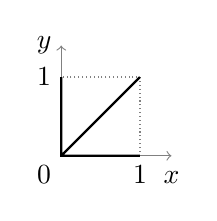
\begin{tikzpicture}
\draw[thin,gray,text=black,<->] (0,1.4) node[left] {$y$}
|- (1.4,0) node[below] {$x\vphantom{1}$};
\draw[densely dotted,gray] (1,0) |- (0,1);
\draw[thick] (0,1) node[left] {$1$} 
-- (0,0) node[below left] {$0$} 
-- (1,0) node[below] {$1$}
(0,0) -- (1,1);
\end{tikzpicture}

\caption{\label{fig:thick-counterexample}Thickness counterexample graph}
\end{figure}


$\Gamma$ is $\beta$-thick because $\rsupfun{\Gamma}\{0\}=[0;1]$.

To prove that $\Gamma$ is not $\alpha$-thick it's enough to prove
that every set $A$ such that $A\times A\subseteq\Gamma$ is finite.

Suppose for the contrary that $A$ is infinite. Then $A$ contains
more than one non-zero points $y$, $z$ ($y\ne z$). Without loss
of generality $y<z$. So we have that $(y,z)$ is not of the form
$(y,y)$ nor $(0,y)$ nor $(y,0)$. Therefore $A\times A$ isn't a
subset of $\Gamma$.
\end{proof}

\section{Totally bounded endoreloids}

The below is a straightforward generalization of the customary definition
of totally bounded sets on uniform spaces (it's proved below that
for uniform spaces the below definitions are equivalent).
\begin{defn}
\index{alpha
-totally bounded@$\alpha$-totally bounded}An endoreloid $f$ is \emph{$\alpha$-totally bounded} ($\totBound_{\alpha}(f)$)
if every~$E\in\up f$ is $\alpha$-thick.
\end{defn}

\begin{defn}
\index{beta
-totally bounded@$\beta$-totally bounded}An endoreloid $f$ is \emph{$\beta$-totally bounded} ($\totBound_{\beta}(f)$)
if every~$E\in\up f$ is $\beta$-thick.\end{defn}
\begin{rem}
We could rewrite the above definitions in a more algebraic way like
$\up f\subseteq\thick_{\alpha}$ (with $\thick_{\alpha}$ would be
defined as a set rather than as a predicate), but we don't really
need this simplification.\end{rem}
\begin{prop}
If an endoreloid is $\alpha$-totally bounded then it is $\beta$-totally
bounded.\end{prop}
\begin{proof}
Because $\thick_{\alpha}(E)\Rightarrow\thick_{\beta}(E)$.\end{proof}
\begin{prop}
If an endoreloid $f$ is reflexive and $\Ob f$ is finite then $f$
is both $\alpha$-totally bounded and $\beta$-totally bounded.\end{prop}
\begin{proof}
It enough to prove that $f$ is $\alpha$-totally bounded. Really,
every $E\in\up f$ is reflexive. Thus $\{x\}\times\{x\}\subseteq\GR E$
for $x\in\Ob f$ and thus $\setcond{\{x\}}{x\in\Ob f}$ is a sought
for finite cover of $\Ob f$.\end{proof}
\begin{obvious}
~
\begin{itemize}
\item A principal endoreloid induced by a $\mathbf{Rel}$-morphism $E$ is
$\alpha$-totally bounded iff $E$ is $\alpha$-thick.
\item A principal endoreloid induced by a $\mathbf{Rel}$-morphism $E$ is
$\beta$-totally bounded iff $E$ is $\beta$-thick.
\end{itemize}
\end{obvious}
\begin{example}
There is a $\beta$-totally bounded endoreloid which is not $\alpha$-totally
bounded.\end{example}
\begin{proof}
It follows from the example above and properties of principal endoreloids.
\end{proof}

\section{Special case of uniform spaces}

Remember that \emph{uniform space} is essentially the same as symmetric,
reflexive and transitive endoreloid.
\begin{thm}
Let $f$ be such an endoreloid that $f\circ f^{-1}\sqsubseteq f$.
Then $f$ is $\alpha$-totally bounded iff it is $\beta$-totally
bounded.\end{thm}
\begin{proof}
~
\begin{description}
\item [{$\Rightarrow$}] Proved above.
\item [{$\Leftarrow$}] For every $\epsilon\in\up f$ we have that $\rsupfun{\GR\epsilon}\{c_{0}\},\dots,\rsupfun{\GR\epsilon}\{c_{n}\}$
covers the space. $\rsupfun{\GR\epsilon}\{c_{i}\}\times\rsupfun{\GR\epsilon}\{c_{i}\}\subseteq\GR(\epsilon\circ\epsilon^{-1})$
because for $x\in\rsupfun{\GR\epsilon}\{c_{i}\}$ (the same as $c_{i}\in\rsupfun{\GR\epsilon}\{x\}$)
we have 
\[
\rsupfun{\rsupfun{\GR\epsilon}\{c_{i}\}\times\rsupfun{\GR\epsilon}\{c_{i}\}}\{x\}=\rsupfun{\GR\epsilon}\{c_{i}\}\subseteq\rsupfun{\GR\epsilon}\rsupfun{\GR\epsilon^{-1}}\{x\}=\rsupfun{\GR(\epsilon\circ\epsilon^{-1})}\{x\}.
\]
For every $\epsilon'\in\up f$ exists $\epsilon\in\up f$ such that
$\epsilon\circ\epsilon^{-1}\sqsubseteq\epsilon'$ because $f\circ f^{-1}\sqsubseteq f$.
Thus for every $\epsilon'$ we have $\rsupfun{\GR\epsilon}\{c_{i}\}\times\rsupfun{\GR\epsilon}\{c_{i}\}\subseteq\GR\epsilon'$
and so $\rsupfun{\GR\epsilon}\{c_{0}\},\dots,\rsupfun{\GR\epsilon}\{c_{n}\}$
is a sought for finite cover.
\end{description}
\end{proof}
\begin{cor}
A uniform space is $\alpha$-totally bounded iff it is $\beta$-totally
bounded.\end{cor}
\begin{proof}
From the theorem and the definition of uniform spaces.
\end{proof}
Thus we can say about just \emph{totally bounded} uniform spaces (without
specifying whether it is $\alpha$ or $\beta$).


\section{Relationships with other properties}
\begin{thm}
Let $\mu$ and $\nu$ be endoreloids. Let $f$ be a principal $\continuous'(\mu,\nu)$
continuous, monovalued, surjective reloid. Then if $\mu$ is $\beta$-totally
bounded then $\nu$ is also $\beta$-totally bounded.\end{thm}
\begin{proof}
Let $\varphi$ be the monovalued, surjective function, which induces
the reloid~$f$.

We have $\mu\sqsubseteq f^{-1}\circ\nu\circ f$.

Let $F\in\up\nu$. Then there exists $E\in\up\mu$ such that $E\subseteq\varphi^{-1}\circ F\circ\varphi$.

Since $\mu$ is $\beta$-totally bounded, there exists a finite typed
subset $A$ of $\Ob\mu$ such that $\rsupfun{\GR E}A=\Ob\mu$.

We claim $\rsupfun{\GR F}\rsupfun{\varphi}A=\Ob\nu$.

Indeed let $y\in\Ob\nu$ be an arbitrary point. Since $\varphi$ is
surjective, there exists $x\in\Ob\mu$ such that $\varphi x=y$. Since
$\rsupfun{\GR E}A=\Ob\mu$ there exists $a\in A$ such that $a\mathrel{(\GR E)}x$
and thus $a\mathrel{(\varphi^{-1}\circ F\circ\varphi)}x$. So $(\varphi a,y)=(\varphi a,\varphi x)\in\GR F$.
Therefore $y\in\rsupfun{\GR F}\rsupfun{\varphi}A$.\end{proof}
\begin{thm}
Let $\mu$ and $\nu$ be endoreloids. Let $f$ be a principal $\continuous''(\mu,\nu)$
continuous, surjective reloid. Then if $\mu$ is $\alpha$-totally
bounded then $\nu$ is also $\alpha$-totally bounded.\end{thm}
\begin{proof}
Let $\varphi$ be the surjective binary relation which induces the
reloid $f$.

We have $f\circ\mu\circ f^{-1}\sqsubseteq\nu$.

Let $F\in\up\nu$. Then there exists $E\in\up\mu$ such that $\varphi\circ E\circ\varphi^{-1}\subseteq F$.

There exists a finite cover $S$ of $\Ob\mu$ such that $\bigcup\setcond{A\times A}{A\in S}\subseteq\GR E$.

Thus $\varphi\circ\left(\bigcup\setcond{A\times A}{A\in S}\right)\circ\varphi^{-1}\subseteq\GR F$
that is $\bigcup\setcond{\rsupfun{\varphi}A\times\rsupfun{\varphi}A}{A\in S}\subseteq\GR F$.

It remains to prove that $\setcond{\rsupfun{\varphi}A}{A\in S}$ is
a cover of $\Ob\nu$. It is true because $\varphi$ is a surjection
and $S$ is a cover of $\Ob\mu$.
\end{proof}
A stronger statement (principality requirement removed):
\begin{conjecture}
The image of a uniformly continuous entirely defined monovalued surjective
reloid from a ($\alpha$-, $\beta$-)totally bounded endoreloid is
also ($\alpha$-, $\beta$-)totally bounded.
\end{conjecture}
Can we remove the requirement to be entirely defined from the above
conjecture?
\begin{question}
Under which conditions it's true that join of ($\alpha$-, $\beta$-)
totally bounded reloids is also totally bounded?
\end{question}

\section{Additional predicates}

We may consider also the following predicates expressing different
kinds of what is intuitively is understood as boundness. Their usefulness
is unclear, but I present them for completeness.
\begin{itemize}
\item $\totBound_{\alpha}(f)$
\item $\totBound_{\beta}(f)$
\item $\exists n\in\mathbb{N}\forall E\in\up f:\thick_{\alpha}(E^{n})$
\item $\exists n\in\mathbb{N}\forall E\in\up f:\thick_{\beta}(E^{n})$
\item $\exists n\in\mathbb{N}\forall E\in\up f:\thick_{\alpha}(E^{0}\sqcup\ldots\sqcup E^{n})$
\item $\exists n\in\mathbb{N}\forall E\in\up f:\thick_{\beta}(E^{0}\sqcup\ldots\sqcup E^{n})$
\item $\exists n\in\mathbb{N}:\totBound_{\alpha}(f^{n})$
\item $\exists n\in\mathbb{N}:\totBound_{\beta}(f^{n})$
\item $\exists n\in\mathbb{N}:\totBound_{\alpha}(f^{0}\sqcup\ldots\sqcup f^{n})$
\item $\exists n\in\mathbb{N}:\totBound_{\beta}(f^{0}\sqcup\ldots\sqcup f^{n})$
\item $\totBound_{\alpha}(S(f))$
\item $\totBound_{\beta}(S(f))$
\end{itemize}
Some of the above defined predicates are equivalent:
\begin{prop}
~
\begin{itemize}
\item $\exists n\in\mathbb{N}\forall E\in\up f:\thick_{\alpha}(E^{n})\Leftrightarrow\exists n\in\mathbb{N}:\totBound_{\alpha}(f^{n})$.
\item $\exists n\in\mathbb{N}\forall E\in\up f:\thick_{\beta}(E^{n})\Leftrightarrow\exists n\in\mathbb{N}:\totBound_{\beta}(f^{n})$.
\end{itemize}
\end{prop}
\begin{proof}
Because for every $E\in\up f$ some $F\in\up f^{n}$ is a subset of $E^{n}$, we have
\[\forall E\in\up f:\thick_{\alpha}(E^{n})\Leftrightarrow\forall F\in\up f^n:\thick_{\alpha}(F)\]
and likewise for $\thick_{\beta}$.\end{proof}
\begin{prop}
~
\begin{itemize}
\item $\exists n\in\mathbb{N}\forall E\in\up f:\thick_{\alpha}(E^{0}\sqcup\ldots\sqcup E^{n})\Leftrightarrow\exists n\in\mathbb{N}:\totBound_{\alpha}(f^{0}\sqcup\ldots\sqcup f^{n})$
\item $\exists n\in\mathbb{N}\forall E\in\up f:\thick_{\beta}(E^{0}\sqcup\ldots\sqcup E^{n})\Leftrightarrow\exists n\in\mathbb{N}:\totBound_{\beta}(f^{0}\sqcup\ldots\sqcup f^{n})$
\end{itemize}
\end{prop}
\begin{proof}
It's enough to prove
\begin{align}
\label{thk-1}&\forall E\in\up f\exists F\in\up(f^0\sqcup\dots\sqcup f^n):F\sqsubseteq E^{0}\sqcup\ldots\sqcup E^{n} \text{ and}\\
\label{thk-2}&\forall F\in\up(f^0\sqcup\dots\sqcup f^n)\exists E\in\up f:E^{0}\sqcup\ldots\sqcup E^{n}\sqsubseteq F.
\end{align}

For the formula~\eqref{thk-1} take $F=E^0\sqcup\dots\sqcup E^n$.

Let's prove~\eqref{thk-2}. Let $F\in\up(f^0\sqcup\dots\sqcup f^n)$. Using the fact that $F\in\up f^i$ take
$E_i\in\up f$ for $i=0,\dots,n$ such that $E_i^i\sqsubseteq F$ (exercise~\ref{rld-fn} and properties of generalized filter bases) and then $E=E_{0}\sqcap\dots\sqcap E_{n}\in\up f$. We have
$E^{0}\sqcup\ldots\sqcup E^{n}\sqsubseteq F$.
\end{proof}
\begin{prop}
All predicates in the above list are pairwise equivalent in the case
if $f$ is a uniform space.\end{prop}
\begin{proof}
Because $f\circ f=f$
and thus $f^n=f^0\sqcup\dots\sqcup f^n=S(f)=f$.\end{proof}


\chapter{Orderings of filters in terms of reloids}

Whilst the other chapters of this book use filters to research funcoids
and reloids, here the opposite thing is discussed, the theory of reloids
is used to describe properties of filters.

In this chapter the word \emph{filter} is used to denote a filter
on a set (not on an arbitrary poset) only.

\section{Ordering of filters}

Below I will define some categories having filters (with possibly
different bases) as their objects and some relations having two filters
(with possibly different bases) as arguments induced by these categories
(defined as existence of a morphism between these two filters).
\begin{thm}
$\card a=\card U$ for every ultrafilter $a$ on $U$ if $U$ is infinite.\end{thm}
\begin{proof}
Let $f(X)=X$ if $X\in a$ and $f(X)=U\setminus X$ if $X\notin a$.
Obviously $f$ is a surjection from $U$ to $a$.

Every $X\in a$ appears as a value of $f$ exactly twice, as $f(X)$
and $f(U\setminus X)$. So $\card a=(\card U)/2=\card U$.\end{proof}
\begin{cor}
Cardinality of every two ultrafilters on a set $U$ is the same.\end{cor}
\begin{proof}
For infinite $U$ it follows from the theorem. For finite case it
is obvious.\end{proof}
\begin{prop}
$\supfun{\uparrow^{\mathsf{FCD}}f}\mathcal{A}=\setcond{C\in\subsets(\Dst f)}{\rsupfun{f^{-1}}C\in\mathcal{A}}$
for every $\mathbf{Set}$-morphism $f:\Base(\mathcal{A})\rightarrow\Base(\mathcal{B})$.
(Here a funcoid is considered as a pair of functions $\mathfrak{F}(\Base(\mathcal{A}))\rightarrow\mathfrak{F}(\Base(\mathcal{B}))$,
$\mathfrak{F}(\Base(\mathcal{B}))\rightarrow\mathfrak{F}(\Base(\mathcal{A}))$
rather than as a pair of functions $\mathscr{F}(\Base(\mathcal{A}))\rightarrow\mathscr{F}(\Base(\mathcal{B}))$,
$\mathscr{F}(\Base(\mathcal{B}))\rightarrow\mathscr{F}(\Base(\mathcal{A}))$.)\end{prop}
\begin{proof}
For every set $C\in\subsets\Base(\mathcal{B})$ we have
\begin{align*}
\rsupfun{f^{-1}}C\in\mathcal{A} & \Rightarrow\\
\exists K\in\mathcal{A}:\rsupfun{f^{-1}}C=K & \Rightarrow\\
\exists K\in\mathcal{A}:\rsupfun f\rsupfun{f^{-1}}C=\rsupfun fK & \Rightarrow\\
\exists K\in\mathcal{A}:C\supseteq\rsupfun fK & \Leftrightarrow\\
\exists K\in\mathcal{A}:C\in\rsupfun{\uparrow^{\mathsf{FCD}}f}K & \Rightarrow\\
C\in\supfun{\uparrow^{\mathsf{FCD}}f}\mathcal{A}.
\end{align*}
So $C\in \setcond{C\in\subsets(\Dst f)}{\rsupfun{f^{-1}}C\in\mathcal{A}}\Rightarrow C\in\supfun{\uparrow^{\mathsf{FCD}}f}\mathcal{A}$.

Let now $C\in\supfun{\uparrow^{\mathsf{FCD}}f}\mathcal{A}$. Then
$\uparrow\rsupfun{f^{-1}}C\sqsupseteq\supfun{\uparrow^{\mathsf{FCD}}f^{-1}}\supfun{\uparrow^{\mathsf{FCD}}f}\mathcal{A}\sqsupseteq\mathcal{A}$
and thus $\rsupfun{f^{-1}}C\in\mathcal{A}$.
\end{proof}
Below I'll define some directed multigraphs. By an abuse of notation,
I will denote these multigraphs the same as (below defined) categories
based on some of these directed multigraphs with added composition
of morphisms (of directed multigraphs edges). As such I will call
vertices of these multigraphs objects and edges morphisms.
\begin{defn}
I will denote $\mathbf{GreFunc}{}_{1}$ the multigraph whose objects
are filters and whose morphisms between objects $\mathcal{A}$ and
$\mathcal{B}$ are $\mathbf{Set}$-morphisms from $\Base(\mathcal{A})$
to $\Base(\mathcal{B})$ such that $\mathcal{B}\sqsubseteq\supfun{\uparrow^{\mathsf{FCD}}f}\mathcal{A}$.
\end{defn}

\begin{defn}
I will denote $\mathbf{GreFunc}{}_{2}$ the multigraph whose objects
are filters and whose morphisms between objects $\mathcal{A}$ and
$\mathcal{B}$ are $\mathbf{Set}$-morphisms from $\Base(\mathcal{A})$
to $\Base(\mathcal{B})$ such that $\mathcal{B}=\supfun{\uparrow^{\mathsf{FCD}}f}\mathcal{A}$.
\end{defn}

\begin{defn}
Let $\mathcal{A}$ be a filter on a set $X$ and $\mathcal{B}$ be
a filter on a set $Y$. $\mathcal{A}\ge_{1}\mathcal{B}$ iff $\Hom_{\mathbf{GreFunc}_{1}}(\mathcal{A},\mathcal{B})$
is not empty.
\end{defn}

\begin{defn}
Let $\mathcal{A}$ be a filter on a set $X$ and $\mathcal{B}$ be
a filter on a set $Y$. $\mathcal{A}\ge_{2}\mathcal{B}$ iff $\Hom_{\mathbf{GreFunc}_{2}}(\mathcal{A},\mathcal{B})$
is not empty.\end{defn}
\begin{prop}
~
\begin{enumerate}
\item \label{gre-imp}$f\in\Hom_{\mathbf{GreFunc}_{1}}(\mathcal{A},\mathcal{B})$
iff $f$ is a $\mathbf{Set}$-morphism from $\Base(\mathcal{A})$
to $\Base(\mathcal{B})$ such that
\[
C\in\mathcal{B}\Leftarrow\rsupfun{f^{-1}}C\in\mathcal{A}
\]
for every $C\in\subsets\Base(\mathcal{B})$.
\item \label{gre-eq}$f\in\Hom_{\mathbf{GreFunc}_{2}}(\mathcal{A},\mathcal{B})$
iff $f$ is a $\mathbf{Set}$-morphism from $\Base(\mathcal{A})$
to $\Base(\mathcal{B})$ such that
\[
C\in\mathcal{B}\Leftrightarrow\rsupfun{f^{-1}}C\in\mathcal{A}
\]
for every $C\in\subsets\Base(\mathcal{B})$.
\end{enumerate}
\end{prop}
\begin{proof}
~
\begin{widedisorder}
\item [{\ref{gre-imp}}] ~
\begin{multline*}
f\in\Hom_{\mathbf{GreFunc}_{1}}(\mathcal{A},\mathcal{B})\Leftrightarrow\mathcal{B}\sqsubseteq\supfun{\uparrow^{\mathsf{FCD}}f}\mathcal{A}\Leftrightarrow\\
\forall C\in\supfun{\uparrow^{\mathsf{FCD}}f}\mathcal{A}:C\in\mathcal{B}\Leftrightarrow\forall C\in\subsets\Base(\mathcal{B}):(\rsupfun{f^{-1}}C\in\mathcal{A}\Rightarrow C\in\mathcal{B}).
\end{multline*}

\item [{\ref{gre-eq}}] ~
\begin{multline*}
f\in\Hom_{\mathbf{GreFunc}_{2}}(\mathcal{A},\mathcal{B})\Leftrightarrow\mathcal{B}=\supfun{\uparrow^{\mathsf{FCD}}f}\mathcal{A}\Leftrightarrow\forall C:(C\in\mathcal{B}\Leftrightarrow C\in\supfun{\uparrow^{\mathsf{FCD}}f}\mathcal{A})\Leftrightarrow\\
\forall C\in\subsets\Base(\mathcal{B}):(C\in\mathcal{B}\Leftrightarrow C\in\supfun{\uparrow^{\mathsf{FCD}}f}\mathcal{A})\Leftrightarrow\\
\forall C\in\subsets\Base(\mathcal{B}):(\rsupfun{f^{-1}}C\in\mathcal{A}\Leftrightarrow C\in\mathcal{B}).
\end{multline*}

\end{widedisorder}
\end{proof}
\begin{defn}
The directed multigraph $\mathbf{FuncBij}$ is the directed multigraph
got from $\mathbf{GreFunc}_{2}$ by restricting to only bijective
morphisms.
\end{defn}

\begin{defn}
\index{directly isomorphic}A filter $\mathcal{A}$ is \emph{directly
isomorphic} to a filter $\mathcal{B}$ iff there is a morphism $f\in\Hom_{\mathbf{FuncBij}}(\mathcal{A},\mathcal{B})$.\end{defn}
\begin{obvious}
$f\in\Hom_{\mathbf{GreFunc}_{1}}(\mathcal{A},\mathcal{B})\Leftrightarrow\mathcal{B}\sqsubseteq\supfun{\uparrow^{\mathsf{FCD}}f}\mathcal{A}$
for every $\mathbf{Set}$-morphism from $\Base(\mathcal{A})$ to $\Base(\mathcal{B})$.
\end{obvious}

\begin{obvious}
$f\in\Hom_{\mathbf{GreFunc}_{2}}(\mathcal{A},\mathcal{B})\Leftrightarrow\mathcal{B}=\supfun{\uparrow^{\mathsf{FCD}}f}\mathcal{A}$
for every $\mathbf{Set}$-morphism from $\Base(\mathcal{A})$ to $\Base(\mathcal{B})$.
\end{obvious}

\begin{cor}
$\mathcal{A}\ge_{1}\mathcal{B}$ iff it exists a $\mathbf{Set}$-morphism
$f:\Base(\mathcal{A})\rightarrow\Base(\mathcal{B})$ such that $\mathcal{B}\sqsubseteq\supfun{\uparrow^{\mathsf{FCD}}f}\mathcal{A}$.
\end{cor}

\begin{cor}
$\mathcal{A}\ge_{2}\mathcal{B}$ iff it exists a $\mathbf{Set}$-morphism
$f:\Base(\mathcal{A})\rightarrow\Base(\mathcal{B})$ such that $\mathcal{B}=\supfun{\uparrow^{\mathsf{FCD}}f}\mathcal{A}$.\end{cor}
\begin{prop}
For a bijective $\mathbf{Set}$-morphism $f:\Base(\mathcal{A})\rightarrow\Base(\mathcal{B})$
the following are equivalent:
\begin{enumerate}
\item \label{fbij-star}$\mathcal{B}=\setcond{C\in\subsets\Base(\mathcal{B})}{\rsupfun{f^{-1}}C\in\mathcal{A}}$.
\item \label{fbij-eback}$\forall C\in\Base(\mathcal{B}):(C\in\mathcal{B}\Leftrightarrow\rsupfun{f^{-1}}C\in\mathcal{A})$.
\item \label{fbij-eforw}$\forall C\in\Base(\mathcal{A}):(C\in\rsupfun f\mathcal{B}\Leftrightarrow C\in\mathcal{A})$.
\item \label{fbij-rbij}$\supfun{\uparrow^{\mathsf{FCD}}f}|_{\mathcal{A}}$
is a bijection from $\mathcal{A}$ to~$\mathcal{B}$.
\item \label{fbij-rsurj}$\supfun{\uparrow^{\mathsf{FCD}}f}|_{\mathcal{A}}$
is a function onto~$\mathcal{B}$.
\item \label{fbij-feq}$\mathcal{B}=\supfun{\uparrow^{\mathsf{FCD}}f}\mathcal{A}$.
\item \label{fbij-gre}$f\in\Hom_{\mathbf{GreFunc}_{2}}(\mathcal{A},\mathcal{B})$.
\item \label{fbij-grp}$f\in\Hom_{\mathbf{FuncBij}}(\mathcal{A},\mathcal{B})$.
\end{enumerate}
\end{prop}
\begin{proof}
~
\begin{description}
\item [{\ref{fbij-star}$\Leftrightarrow$\ref{fbij-eback}}] ~
\[
\mathcal{B}=\setcond{C\in\subsets\Base(\mathcal{B})}{\rsupfun{f^{-1}}C\in\mathcal{A}}\Leftrightarrow\\
\forall C\in\subsets\Base(\mathcal{B}):(C\in\mathcal{B}\Leftrightarrow\rsupfun{f^{-1}}C\in\mathcal{A}).
\]

\item [{\ref{fbij-eback}$\Leftrightarrow$\ref{fbij-eforw}}] Because
$f$ is a bijection.
\item [{\ref{fbij-eback}$\Rightarrow$\ref{fbij-rsurj}}] For every $C\in\mathcal{B}$
we have $\rsupfun{f^{-1}}C\in\mathcal{A}$ and thus $\supfun{\uparrow^{\mathsf{FCD}}f}|_{\mathcal{A}}\supfun{\uparrow^{\mathsf{FCD}}f^{-1}}C=\rsupfun f\rsupfun{f^{-1}}C=C$.
Thus $\supfun{\uparrow^{\mathsf{FCD}}f}|_{\mathcal{A}}$ is onto $\mathcal{B}$.
\item [{\ref{fbij-rbij}$\Rightarrow$\ref{fbij-rsurj}}] Obvious.
\item [{\ref{fbij-rsurj}$\Rightarrow$\ref{fbij-rbij}}] We need to prove
only that $\supfun{\uparrow^{\mathsf{FCD}}f}|_{\mathcal{A}}$ is an
injection. But this follows from the fact that $f$ is a bijection.
\item [{\ref{fbij-rbij}$\Rightarrow$\ref{fbij-eforw}}] We have $\forall C\in\Base(\mathcal{A}):((\supfun{\uparrow^{\mathsf{FCD}}f}|_{\mathcal{A}})C\in\mathcal{B}\Leftrightarrow C\in\mathcal{A})$
and consequently $\forall C\in\Base(\mathcal{A}):(\rsupfun fC\in\mathcal{B}\Leftrightarrow C\in\mathcal{A})$.
\item [{\ref{fbij-feq}$\Leftrightarrow$\ref{fbij-star}}] From the last
corollary.
\item [{\ref{fbij-star}$\Leftrightarrow$\ref{fbij-gre}}] Obvious.
\item [{\ref{fbij-gre}$\Leftrightarrow$\ref{fbij-grp}}] Obvious.
\end{description}
\end{proof}
\begin{cor}
The following are equivalent for every filters $\mathcal{A}$ and
$\mathcal{B}$:
\begin{enumerate}
\item $\mathcal{A}$ is directly isomorphic to $\mathcal{B}$.
\item There is a bijective $\mathbf{Set}$-morphism $f:\Base(\mathcal{A})\rightarrow\Base(\mathcal{B})$
such that for every $C\in\mathscr{P}\Base(\mathcal{B})$
\[
C\in\mathcal{B}\Leftrightarrow\rsupfun{f^{-1}}C\in\mathcal{A}.
\]

\item There is a bijective $\mathbf{Set}$-morphism $f:\Base(\mathcal{A})\rightarrow\Base(\mathcal{B})$
such that for every $C\in\mathscr{P}\Base(\mathcal{B})$
\[
\rsupfun fC\in\mathcal{B}\Leftrightarrow C\in\mathcal{A}.
\]

\item There is a bijective $\mathbf{Set}$-morphism $f:\Base(\mathcal{A})\rightarrow\Base(\mathcal{B})$
such that $\supfun{\uparrow^{\mathsf{FCD}}f}|_{\mathcal{A}}$ is a
bijection from $\mathcal{A}$ to $\mathcal{B}$.
\item There is a bijective $\mathbf{Set}$-morphism $f:\Base(\mathcal{A})\rightarrow\Base(\mathcal{B})$
such that $\supfun{\uparrow^{\mathsf{FCD}}f}|_{\mathcal{A}}$ is a
function onto $\mathcal{B}$.
\item There is a bijective $\mathbf{Set}$-morphism $f:\Base(\mathcal{A})\rightarrow\Base(\mathcal{B})$
such that $\mathcal{B}=\supfun{\uparrow^{\mathsf{FCD}}f}\mathcal{A}$.
\item There is a bijective morphism $f\in\Hom_{\mathbf{GreFunc}_{2}}(\mathcal{A},\mathcal{B})$.
\item There is a bijective morphism $f\in\Hom_{\mathbf{FuncBij}}(\mathcal{A},\mathcal{B})$.
\end{enumerate}
\end{cor}
\begin{prop}
$\mathbf{GreFunc}_{1}$ and $\mathbf{GreFunc}_{2}$ with function
composition are categories.\end{prop}
\begin{proof}
Let $f:\mathcal{A}\rightarrow\mathcal{B}$ and $g:\mathcal{B}\rightarrow\mathcal{C}$
be morphisms of $\mathbf{GreFunc}_{1}$. Then $\mathcal{B}\sqsubseteq\supfun{\uparrow^{\mathsf{FCD}}f}\mathcal{A}$
and $\mathcal{C}\sqsubseteq\supfun{\uparrow^{\mathsf{FCD}}g}\mathcal{B}$.
So 
\[
\supfun{\uparrow^{\mathsf{FCD}}(g\circ f)}\mathcal{A}=\supfun{\uparrow^{\mathsf{FCD}}g}\supfun{\uparrow^{\mathsf{FCD}}f}\mathcal{A}\sqsupseteq\supfun{\uparrow^{\mathsf{FCD}}g}\mathcal{B}\sqsupseteq\mathcal{C}.
\]
Thus $g\circ f$ is a morphism of $\mathbf{GreFunc}_{1}$. Associativity
law is evident. $\id_{\Base(\mathcal{A})}$ is the identity morphism
of $\mathbf{GreFunc}_{1}$ for every filter~$\mathcal{A}$.

Let $f:\mathcal{A}\rightarrow\mathcal{B}$ and $g:\mathcal{B}\rightarrow\mathcal{C}$
be morphisms of $\mathbf{GreFunc}_{2}$. Then $\mathcal{B}=\supfun{\uparrow^{\mathsf{FCD}}f}\mathcal{A}$
and $\mathcal{C}=\supfun{\uparrow^{\mathsf{FCD}}g}\mathcal{B}$. So
\[
\supfun{\uparrow^{\mathsf{FCD}}(g\circ f)}\mathcal{A}=\supfun{\uparrow^{\mathsf{FCD}}g}\supfun{\uparrow^{\mathsf{FCD}}f}\mathcal{A}=\supfun{\uparrow^{\mathsf{FCD}}g}\mathcal{B}=\mathcal{C}.
\]
Thus $g\circ f$ is a morphism of $\mathbf{GreFunc}_{2}$. Associativity
law is evident. $\id_{\Base(\mathcal{A})}$ is the identity morphism
of $\mathbf{GreFunc}_{2}$ for every filter~$\mathcal{A}$.\end{proof}
\begin{cor}
$\le_{1}$ and $\le_{2}$ are preorders. \end{cor}
\begin{thm}
$\mathbf{FuncBij}$ is a groupoid.\end{thm}
\begin{proof}
First let's prove it is a category. Let $f:\mathcal{A}\rightarrow\mathcal{B}$
and $g:\mathcal{B}\rightarrow\mathcal{C}$ be morphisms of $\mathbf{FuncBij}$.
Then $f:\Base(\mathcal{A})\rightarrow\Base(\mathcal{B})$ and $g:\Base(\mathcal{B})\rightarrow\Base(\mathcal{C})$
are bijections and $\mathcal{B}=\supfun{\uparrow^{\mathsf{FCD}}f}\mathcal{A}$
and $\mathcal{C}=\supfun{\uparrow^{\mathsf{FCD}}g}\mathcal{B}$. Thus
$g\circ f:\Base(\mathcal{A})\rightarrow\Base(\mathcal{C})$ is a bijection
and $\mathcal{C}=\supfun{\uparrow^{\mathsf{FCD}}(g\circ f)}\mathcal{A}$.
Thus $g\circ f$ is a morphism of $\mathbf{FuncBij}$. $\id_{\Base(\mathcal{A})}$
is the identity morphism of $\mathbf{FuncBij}$ for every filter $\mathcal{A}$.
Thus it is a category.

It remains to prove only that every morphism $f\in\Hom_{\mathbf{FuncBij}}(\mathcal{A},\mathcal{B})$
has a reverse (for every filters $\mathcal{A}$, $\mathcal{B}$).
We have $f$ is a bijection $\Base(\mathcal{A})\rightarrow\Base(\mathcal{B})$
such that for every $C\in\subsets\Base(\mathcal{A})$
\[
\rsupfun fC\in\mathcal{B}\Leftrightarrow C\in\mathcal{A}.
\]
Then $f^{-1}:\Base(\mathcal{B})\rightarrow\Base(\mathcal{A})$ is
a bijection such that for every $C\in\subsets\Base(\mathcal{B})$
\[
\rsupfun{f^{-1}}C\in\mathcal{A}\Leftrightarrow C\in\mathcal{B}.
\]
 Thus $f^{-1}\in\Hom_{\mathbf{FuncBij}}(\mathcal{B},\mathcal{A})$.\end{proof}
\begin{cor}
Being directly isomorphic is an equivalence relation.
\end{cor}
\index{order!Rudin-Keisler}Rudin-Keisler order of ultrafilters is
considered in such a book as \cite{comfort-ultra}.
\begin{obvious}
For the case of ultrafilters being directly isomorphic is the same
as being Rudin-Keisler equivalent.\end{obvious}
\begin{defn}
\index{isomorphic!filters}A filter $\mathcal{A}$ is \emph{isomorphic}
to a filter $\mathcal{B}$ iff there exist sets $A\in\mathcal{A}$
and $B\in\mathcal{B}$ such that $\mathcal{A}\div A$ is directly
isomorphic to $\mathcal{B}\div B$.\end{defn}
\begin{obvious}
Equivalent filters are isomorphic.\end{obvious}
\begin{thm}
Being isomorphic (for small filters) is an equivalence relation.\end{thm}
\begin{proof}
~
\begin{description}
\item [{Reflexivity}] Because every filter is directly isomorphic to itself.
\item [{Symmetry}] If filter $\mathcal{A}$ is isomorphic to $\mathcal{B}$
then there exist sets $A\in\mathcal{A}$ and $B\in\mathcal{B}$ such
that $\mathcal{A}\div A$ is directly isomorphic to $\mathcal{B}\div B$
and thus $\mathcal{B}\div B$ is directly isomorphic to $\mathcal{A}\div A$.
So $\mathcal{B}$ is isomorphic to $\mathcal{A}$.
\item [{Transitivity}] Let $\mathcal{A}$ be isomorphic to $\mathcal{B}$
and $\mathcal{B}$ be isomorphic to $\mathcal{C}$. Then exist $A\in\mathcal{A}$,
$B_{1}\in\mathcal{B}$, $B_{2}\in\mathcal{B}$, $C\in\mathcal{C}$
such that there are bijections $f:A\rightarrow B_{1}$ and $g:B_{2}\rightarrow C$
such that
\[
\forall X\in\subsets A:(X\in\mathcal{B}\Leftrightarrow\rsupfun{f^{-1}}X\in\mathcal{A})\quad\text{and}\quad\forall X\in\subsets B_{1}:(X\in\mathcal{A}\Leftrightarrow\rsupfun fX\in\mathcal{B})
\]
and also $\forall X\in\subsets B_{2}:(X\in\mathcal{B}\Leftrightarrow\rsupfun gX\in\mathcal{C})$.


So $g\circ f$ is a bijection from $\rsupfun{f^{-1}}(B_{1}\cap B_{2})\in\mathcal{A}$
to $\rsupfun g(B_{1}\cap B_{2})\in\mathcal{C}$ such that
\[
X\in\mathcal{A}\Leftrightarrow\rsupfun fX\in\mathcal{B}\Leftrightarrow\rsupfun g\rsupfun fX\in\mathcal{C}\Leftrightarrow\rsupfun{g\circ f}X\in\mathcal{C}.
\]
Thus $g\circ f$ establishes a bijection which proves that $\mathcal{A}$
is isomorphic to~$\mathcal{C}$.

\end{description}
\end{proof}
\begin{lem}
Let $\card X=\card Y$, $u$ be an ultrafilter on $X$ and $v$ be
an ultrafilter on $Y$; let $A\in u$ and $B\in v$. Let $u\div A$
and $v\div B$ be directly isomorphic. Then if $\card(X\setminus A)=\card(Y\setminus B)$
we have $u$ and $v$ directly isomorphic.\end{lem}
\begin{proof}
Arbitrary extend the bijection witnessing being directly isomorphic
to the sets $X\setminus A$ and $X\setminus B$.\end{proof}
\begin{thm}
If $\card X=\card Y$ then being isomorphic and being directly isomorphic
are the same for ultrafilters $u$ on $X$ and $v$ on $Y$.\end{thm}
\begin{proof}
That if two filters are isomorphic then they are directly isomorphic
is obvious.

Let ultrafilters $u$ and $v$ be isomorphic that is there is a bijection
$f:A\rightarrow B$ where $A\in u$, $B\in v$ witnessing isomorphism
of $u$ and $v$.

If one of the filters $u$ or $v$ is a trivial ultrafilter then the
other is also a trivial ultrafilter and as it is easy to show they
are directly isomorphic. So we can assume $u$ and $v$ are not trivial
ultrafilters.

If $\card(X\setminus A)=\card(Y\setminus B)$ our statement follows
from the last lemma.

Now assume without loss of generality $\card(X\setminus A)<\card(Y\setminus B)$.

$\card B=\card Y$ because otherwise $\card(X\setminus A)=\card(Y\setminus B)$.

It is easy to show that there exists $B'\supset B$ such that $\card(X\setminus A)=\card(Y\setminus B')$
and $\card B'=\card B$.

We will find a bijection $g$ from $B$ to $B'$ which witnesses direct
isomorphism of $v$ to $v$ itself. Then the composition $g\circ f$
witnesses a direct isomorphism of $u\div A$ and $v\div B'$ and by
the lemma $u$ and $v$ are directly isomorphic.

Let $D=B'\setminus B$. We have $D\notin v$.

There exists a set $E\subseteq B$ such that $\card E\ge\card D$
and $E\notin v$.

We have $\card E=\card(D\cup E)$ and thus there exists a bijection
$h:E\rightarrow D\cup E$.

Let
\[
g(x)=\begin{cases}
x & \text{if }x\in B\setminus E;\\
h(x) & \text{if }x\in E.
\end{cases}
\]


$g|_{B\setminus E}$ and $g|_{E}$ are bijections.

$\im(g|_{B\setminus E})=B\setminus E$; $\im(g|_{E})=\im h=D\cup E$;
\[
(D\cup E)\cap(B\setminus E)=(D\cap(B\setminus E))\cup(E\cap(B\setminus E))=\emptyset\cup\emptyset=\emptyset.
\]
Thus $g$ is a bijection from $B$ to $(B\setminus E)\cup(D\cup E)=B\cup D=B'$.

To finish the proof it's enough to show that $\rsupfun gv=v$. Indeed
it follows from $B\setminus E\in v$.\end{proof}
\begin{prop}
~
\begin{enumerate}
\item \label{ge2-restr}For every $A\in\mathcal{A}$ and $B\in\mathcal{B}$
we have $\mathcal{A}\ge_{2}\mathcal{B}$ iff $\mathcal{A}\div A\ge_{2}\mathcal{B}\div B$.
\item \label{ge1-restr}For every $A\in\mathcal{A}$ and $B\in\mathcal{B}$
we have $\mathcal{A}\ge_{1}\mathcal{B}$ iff $\mathcal{A}\div A\ge_{1}\mathcal{B}\div B$.
\end{enumerate}
\end{prop}
\begin{proof}
~
\begin{widedisorder}
\item [{\ref{ge2-restr}}] $\mathcal{A}\ge_{2}\mathcal{B}$ iff there exist
a bijective $\mathbf{Set}$-morphism $f$ such that $\mathcal{B}=\supfun{\uparrow^{\mathsf{FCD}}f}\mathcal{A}$.
The equality is obviously preserved replacing $\mathcal{A}$ with
$\mathcal{A}\div A$ and $\mathcal{B}$ with $\mathcal{B}\div B$.
\item [{\ref{ge1-restr}}] $\mathcal{A}\ge_{1}\mathcal{B}$ iff there exist
a bijective $\mathbf{Set}$-morphism $f$ such that $\mathcal{B}\subseteq\supfun{\uparrow^{\mathsf{FCD}}f}\mathcal{A}$.
The equality is obviously preserved replacing $\mathcal{A}$ with
$\mathcal{A}\div A$ and $\mathcal{B}$ with $\mathcal{B}\div B$.
\end{widedisorder}
\end{proof}
\begin{prop}
For ultrafilters $\ge_{2}$ is the same as Rudin-Keisler ordering
(as defined in \cite{comfort-ultra}).\end{prop}
\begin{proof}
$x\ge_{2}y$ iff there exist sets $A\in x$ and $B\in y$ and a bijective
$\mathbf{Set}$-morphism $f:X\rightarrow Y$ such that
\[
y\div B=\setcond{C\in\subsets Y}{\rsupfun{f^{-1}}C\in x\div A}
\]
 that is when $C\in y\div B\Leftrightarrow\rsupfun{f^{-1}}C\in x\div A$
what is equivalent to~$C\in y\Leftrightarrow\rsupfun{f^{-1}}C\in x$
what is the definition of Rudin-Keisler ordering.\end{proof}
\begin{rem}
\index{Rudin-Keisler equivalence}The relation of being isomorphic
for ultrafilters is traditionally called \emph{Rudin-Keisler equivalence}.\end{rem}
\begin{obvious}
$(\ge_{1})\supseteq(\ge_{2})$.\end{obvious}
\begin{defn}
Let $Q$ and $R$ be binary relations on the set of (small) filters. I will
denote $\mathbf{MonRld}_{Q,R}$ the directed multigraph with objects
being filters and morphisms such monovalued reloids $f$ that $(\dom f)\mathrel Q\mathcal{A}$
and $(\im f)\mathrel R\mathcal{B}$.

I will also denote $\mathbf{CoMonRld}_{Q,R}$ the directed multigraph
with objects being filters and morphisms such injective reloids $f$
that $(\im f)\mathrel Q\mathcal{A}$ and $(\dom f)\mathrel R\mathcal{B}$.
These are essentially the duals.
\end{defn}
Some of these directed multigraphs are categories with reloid composition
(see below). By abuse of notation I will denote these categories the
same as these directed multigraphs.

\begin{lem}
$\mathbf{CoMonRld}_{Q,R}\ne\emptyset \Leftrightarrow\mathbf{MonRld}_{Q,R}\ne\emptyset$.
\end{lem}
\begin{proof}
\begin{multline*}
f\in\mathbf{CoMonRld}_{Q,R} \Leftrightarrow
(\im f)\mathrel Q\mathcal{A} \land (\dom f)\mathrel R\mathcal{B} \Leftrightarrow \\
(\dom f^{-1})\mathrel Q\mathcal{A} \land (\im f^{-1})\mathrel R\mathcal{B} \Leftrightarrow
f^{-1}\in\mathbf{MonRld}_{Q,R}
\end{multline*}
for every monovalued reloid~$f$ (or what is the same, injective reloid~$f^{-1}$).
\end{proof}

\begin{thm}
For every filters $\mathcal{A}$ and $\mathcal{B}$ the following
are equivalent:
\begin{enumerate}
\item \label{ge1-ineq}$\mathcal{A}\ge_{1}\mathcal{B}$.
\item \label{ge1-eq-ge}$\Hom_{\mathbf{MonRld}_{=,\sqsupseteq}}(\mathcal{A},\mathcal{B})\ne\emptyset$.
\item \label{ge1-le-ge}$\Hom_{\mathbf{MonRld}_{\sqsubseteq,\sqsupseteq}}(\mathcal{A},\mathcal{B})\ne\emptyset$.
\item \label{ge1-le-eq}$\Hom_{\mathbf{MonRld}_{\sqsubseteq,=}}(\mathcal{A},\mathcal{B})\ne\emptyset$.
\item \label{g1-c-eq-ge}$\Hom_{\mathbf{CoMonRld}_{=,\sqsupseteq}}(\mathcal{A},\mathcal{B})\ne\emptyset$.
\item \label{g1-c-le-ge}$\Hom_{\mathbf{CoMonRld}_{\sqsubseteq,\sqsupseteq}}(\mathcal{A},\mathcal{B})\ne\emptyset$.
\item \label{g1-c-le-eq}$\Hom_{\mathbf{CoMonRld}_{\sqsubseteq,=}}(\mathcal{A},\mathcal{B})\ne\emptyset$.
\end{enumerate}
\end{thm}
\begin{proof}
~
\begin{description}
\item [{\ref{ge1-ineq}$\Rightarrow$\ref{ge1-eq-ge}}] There exists a
$\mathbf{Set}$-morphism $f:\Base(\mathcal{A})\rightarrow\Base(\mathcal{B})$
such that $\mathcal{B}\sqsubseteq\supfun{\uparrow^{\mathsf{FCD}}f}\mathcal{A}$.
We have
\[
\dom(\uparrow^{\mathsf{RLD}}f)|_{\mathcal{A}}=\mathcal{A}\sqcap\top(\Base(\mathcal{A}))=\mathcal{A}
\]
and
\[
\im(\uparrow^{\mathsf{RLD}}f)|_{\mathcal{A}}=\im\tofcd(\uparrow^{\mathsf{RLD}}f)|_{\mathcal{A}}=\im(\uparrow^{\mathsf{FCD}}f)|_{\mathcal{A}}=\supfun{\uparrow^{\mathsf{FCD}}f}\mathcal{A}\sqsupseteq\mathcal{B}.
\]
Thus $(\uparrow^{\mathsf{RLD}}f)|_{\mathcal{A}}$ is a monovalued
reloid such that $\dom(\uparrow^{\mathsf{RLD}}f)|_{\mathcal{A}}=\mathcal{A}$
and $\im(\uparrow^{\mathsf{RLD}}f)|_{\mathcal{A}}\sqsupseteq\mathcal{B}$.
\item [{\ref{ge1-eq-ge}$\Rightarrow$\ref{ge1-le-ge},~\ref{ge1-le-eq}$\Rightarrow$\ref{ge1-le-ge},~\ref{g1-c-eq-ge}$\Rightarrow$\ref{g1-c-le-ge},~\ref{g1-c-le-eq}$\Rightarrow$\ref{g1-c-le-ge}}] Obvious.
\item [{\ref{ge1-le-ge}$\Rightarrow$\ref{ge1-ineq}}] We have $\mathcal{B}\sqsubseteq\supfun{\tofcd f}\mathcal{A}$
for a monovalued reloid $f\in\mathsf{RLD}(\Base(\mathcal{A}),\Base(\mathcal{B}))$.
Then there exists a $\mathbf{Set}$-morphism $F:\Base(\mathcal{A})\rightarrow\Base(\mathcal{B})$
such that $\mathcal{B}\sqsubseteq\supfun{\uparrow^{\mathsf{FCD}}F}\mathcal{A}$
that is $\mathcal{A}\ge_{1}\mathcal{B}$.
\item [{\ref{g1-c-le-ge}$\Rightarrow$\ref{g1-c-le-eq}}] Let $f$ be an injective reloid such that
$\im f\sqsubseteq\mathcal{A}$ and $\dom f\sqsupseteq\mathcal{B}$. Then
$\im f|_{\mathcal{B}}\sqsubseteq\mathcal{A}$ and $\dom f|_{\mathcal{B}}=\mathcal{B}$.
So $f|_{\mathcal{B}}\in\Hom_{\mathbf{CoMonRld}_{\sqsubseteq,=}}(\mathcal{A},\mathcal{B})$.
\item [{\ref{ge1-eq-ge}$\Leftrightarrow$\ref{g1-c-eq-ge},~\ref{ge1-le-ge}$\Leftrightarrow$\ref{g1-c-le-ge},~\ref{ge1-le-eq}$\Leftrightarrow$\ref{g1-c-le-eq}}] By
the lemma.
\end{description}
\end{proof}
\begin{thm}
For every filters $\mathcal{A}$ and $\mathcal{B}$ the following
are equivalent:
\begin{enumerate}
\item \label{ge2-in}$\mathcal{A}\ge_{2}\mathcal{B}$.
\item \label{ge2-mon}$\Hom_{\mathbf{MonRld}_{=,=}}(\mathcal{A},\mathcal{B})\ne\emptyset$.
\item \label{ge2-comon}$\Hom_{\mathbf{CoMonRld}_{=,=}}(\mathcal{A},\mathcal{B})\ne\emptyset$.
\end{enumerate}
\end{thm}
\begin{proof}
~
\begin{description}
\item [{\ref{ge2-in}$\Rightarrow$\ref{ge2-mon}}] Let $\mathcal{A}\ge_{2}\mathcal{B}$
that is $\mathcal{B}=\supfun{\uparrow^{\mathsf{FCD}}f}\mathcal{A}$
for some $\mathbf{Set}$-morphism $f:\Base(\mathcal{A})\rightarrow\Base(\mathcal{B})$.
Then $\dom(\uparrow^{\mathsf{RLD}}f)|_{\mathcal{A}}=\mathcal{A}$
and 
\[
\im(\uparrow^{\mathsf{RLD}}f)|_{\mathcal{A}}=\im\tofcd(\uparrow^{\mathsf{RLD}}f)|_{\mathcal{A}}=\im(\uparrow^{\mathsf{FCD}}f)|_{\mathcal{A}}=\supfun{\uparrow^{\mathsf{FCD}}f}\mathcal{A}=\mathcal{B}.
\]
So $(\uparrow^{\mathsf{RLD}}f)|_{\mathcal{A}}$ is a sought for reloid.
\item [{\ref{ge2-mon}$\Rightarrow$\ref{ge2-in}}] There exists a monovalued reloid~$f$ with domain~$\mathcal{A}$
such that $\supfun{\tofcd f}\mathcal{A}=\mathcal{B}$.
By corollary \ref{mv-is-restr}
below, there exists a $\mathbf{Set}$-morphism $F:\Base(\mathcal{A})\rightarrow\Base(\mathcal{B})$
such that $f=(\uparrow^{\mathsf{RLD}}F)|_{\mathcal{A}}$. Thus
\[
\supfun{\uparrow^{\mathsf{FCD}}F}\mathcal{A}=\im(\uparrow^{\mathsf{FCD}}F)|_{\mathcal{A}}=\im\tofcd(\uparrow^{\mathsf{RLD}}F)|_{\mathcal{A}}=\im\tofcd f=\im f=\mathcal{B}.
\]
Thus $\mathcal{A}\ge_{2}\mathcal{B}$ is testified by the morphism
$F$.
\item [{\ref{ge2-mon}$\Leftrightarrow$\ref{ge2-comon}}] By the lemma.
\end{description}
\end{proof}
\begin{thm}
The following are categories (with reloid composition):
\begin{enumerate}
\item \label{monrld-le-ge}$\mathbf{MonRld}_{\sqsubseteq,\sqsupseteq}$;
\item \label{monrld-le-eq}$\mathbf{MonRld}_{\sqsubseteq,=}$;
\item \label{monrld-eq-eq}$\mathbf{MonRld}_{=,=}$;
\item $\mathbf{CoMonRld}_{\sqsubseteq,\sqsupseteq}$;
\item $\mathbf{CoMonRld}_{\sqsubseteq,=}$;
\item $\mathbf{CoMonRld}_{=,=}$.
\end{enumerate}
\end{thm}
\begin{proof}
We will prove only the first three. The rest follow from duality.
We need to prove only that composition of morphisms is a morphism,
because associativity and existence of identity morphism are evident.
We have:
\begin{widedisorder}
\item [{\ref{monrld-le-ge}}] Let $f\in\Hom_{\mathbf{MonRld}_{\sqsubseteq,\sqsupseteq}}(\mathcal{A},\mathcal{B})$,
$g\in\Hom_{\mathbf{MonRld}_{\sqsubseteq,\sqsupseteq}}(\mathcal{B},\mathcal{C})$.
Then $\dom f\sqsubseteq\mathcal{A}$, $\im f\sqsupseteq\mathcal{B}$,
$\dom g\sqsubseteq\mathcal{B}$, $\im g\sqsupseteq\mathcal{C}$. So
$\dom(g\circ f)\sqsubseteq\mathcal{A}$, $\im(g\circ f)\sqsupseteq\mathcal{C}$
that is $g\circ f\in\Hom_{\mathbf{MonRld}_{\sqsubseteq,\sqsupseteq}}(\mathcal{A},\mathcal{C})$.
\item [{\ref{monrld-le-eq}}] Let $f\in\Hom_{\mathbf{MonRld}_{\sqsubseteq,=}}(\mathcal{A},\mathcal{B})$,
$g\in\Hom_{\mathbf{MonRld}_{\sqsubseteq,=}}(\mathcal{B},\mathcal{C})$.
Then $\dom f\sqsubseteq\mathcal{A}$, $\im f=\mathcal{B}$, $\dom g\sqsubseteq\mathcal{B}$,
$\im g=\mathcal{C}$. So $\dom(g\circ f)\sqsubseteq\mathcal{A}$,
$\im(g\circ f)=\mathcal{C}$ that is $g\circ f\in\Hom_{\mathbf{MonRld}_{\sqsubseteq,=}}(\mathcal{A},\mathcal{C})$.
\item [{\ref{monrld-eq-eq}}] Let $f\in\Hom_{\mathbf{MonRld}_{=,=}}(\mathcal{A},\mathcal{B})$,
$g\in\Hom_{\mathbf{MonRld}_{=,=}}(\mathcal{B},\mathcal{C})$. Then
$\dom f=\mathcal{A}$, $\im f=\mathcal{B}$, $\dom g=\mathcal{B}$,
$\im g=\mathcal{C}$. So $\dom(g\circ f)=\mathcal{A}$, $\im(g\circ f)=\mathcal{C}$
that is $g\circ f\in\Hom_{\mathbf{MonRld}_{=,=}}(\mathcal{A},\mathcal{C})$.
\end{widedisorder}
\end{proof}
\begin{defn}
Let $\mathbf{BijRld}$ be the groupoid of all bijections of the category
of reloid triples. Its objects are filters and its morphisms from
a filter $\mathcal{A}$ to filter $\mathcal{B}$ are monovalued injective
reloids $f$ such that $\dom f=\mathcal{A}$ and $\im f=\mathcal{B}$.\end{defn}
\begin{thm}
Filters $\mathcal{A}$ and $\mathcal{B}$ are isomorphic iff $\Hom_{\mathbf{BijRld}}(\mathcal{A},\mathcal{B})\neq\emptyset$.\end{thm}
\begin{proof}
~
\begin{description}
\item [{$\Rightarrow$}] Let $\mathcal{A}$ and $\mathcal{B}$ be isomorphic.
Then there are sets $A\in\mathcal{A}$, $B\in\mathcal{B}$ and a bijective
$\mathbf{Set}$-morphism $F:A\rightarrow B$ such that $\rsupfun F:\subsets A\cap\mathcal{A}\rightarrow\subsets B\cap\mathcal{B}$
is a bijection.


Obviously $f=(\uparrow^{\mathsf{RLD}}F)|_{\mathcal{A}}$ is monovalued
and injective.
\begin{align*}
\im f & =\\
\bigsqcap^{\mathfrak{F}}\setcond{\im G}{G\in\up(\uparrow^{\mathsf{RLD}}F)|_{\mathcal{A}}} & =\\
\bigsqcap^{\mathfrak{F}}\setcond{\im(H\cap F|_{X})}{H\in\up(\uparrow^{\mathsf{RLD}}F)|_{\mathcal{A}},X\in\mathcal{A}} & =\\
\bigsqcap^{\mathfrak{F}}\setcond{\im F|_{P}}{P\in\mathcal{A}} & =\\
\bigsqcap^{\mathfrak{F}}\setcond{\rsupfun FP}{P\in\mathcal{A}} & =\\
\bigsqcap^{\mathfrak{F}}\setcond{\rsupfun FP}{P\in\subsets A\cap\mathcal{A}} & =\\
\bigsqcap^{\mathfrak{F}}(\subsets B\cap\mathcal{B}) & =\\
\bigsqcap^{\mathfrak{F}}\mathcal{B}=\mathcal{B}.
\end{align*}
Thus $\dom f=\mathcal{A}$ and $\im f=\mathcal{B}$.

\item [{$\Leftarrow$}] Let $f$ be a monovalued injective reloid such
that $\dom f=\mathcal{A}$ and $\im f=\mathcal{B}$. Then there exist
a function $F'$ and an injective binary relation $F''$ such that
$F',F''\in f$. Thus $F=F'\cap F''$ is an injection such that $F\in f$.
The function $F$ is a bijection from $A=\dom F$ to $B=\im F$. The
function $\rsupfun F$ is an injection on $\subsets A\cap\mathcal{A}$
(and moreover on $\subsets A$). It's simple to show that $\forall X\in\subsets A\cap\mathcal{A}:\rsupfun FX\in\subsets B\cap\mathcal{B}$
and similarly 
\[
\forall Y\in\subsets B\cap\mathcal{B}:(\rsupfun F)^{-1}Y=\rsupfun{F^{-1}}Y\in\subsets A\cap\mathcal{A}.
\]
Thus $\rsupfun F|_{\subsets A\cap\mathcal{A}}$ is a bijection $\subsets A\cap\mathcal{A}\rightarrow\subsets B\cap\mathcal{B}$.
So filters $\mathcal{A}$ and $\mathcal{B}$ are isomorphic.
\end{description}
\end{proof}
\begin{prop}
$(\ge_{1})=(\sqsupseteq)\circ(\ge_{2})$ (when we limit to small filters).\end{prop}
\begin{proof}
$\mathcal{A}\ge_{1}\mathcal{B}$ iff exists a function $f:\Base(\mathcal{A})\rightarrow\Base(\mathcal{B})$
such that $\mathcal{B}\sqsubseteq\supfun{\uparrow^{\mathsf{FCD}}f}\mathcal{A}$.
But $\mathcal{B}\sqsubseteq\supfun{\uparrow^{\mathsf{FCD}}f}\mathcal{A}$
is equivalent to $\exists\mathcal{B}'\in\mathscr{F}:(\mathcal{B}'\sqsupseteq\mathcal{B}\land\mathcal{B}'=\supfun{\uparrow^{\mathsf{FCD}}f}\mathcal{A})$.
So $\mathcal{A}\ge_{1}\mathcal{B}$ is equivalent to existence of
$\mathcal{B}'\in\mathscr{F}$ such that $\mathcal{B}'\sqsupseteq\mathcal{B}$
and existence of a function $f:\Base(\mathcal{A})\rightarrow\Base(\mathcal{B})$
such that $\mathcal{B}'=\supfun{\uparrow^{\mathsf{FCD}}f}\mathcal{A}$.
This is equivalent to $\mathcal{A}\mathrel{((\sqsupseteq)\circ(\ge_{2}))}\mathcal{B}$.\end{proof}
\begin{prop}
If $a$ and $b$ are ultrafilters then $b\ge_{1}a\Leftrightarrow b\ge_{2}a$.\end{prop}
\begin{proof}
We need to prove only $b\ge_{1}a\Rightarrow b\ge_{2}a$. If $b\ge_{1}a$
then there exists a monovalued reloid $f:\Base(b)\rightarrow\Base(a)$
such that $\dom f=b$ and $\im f\sqsupseteq a$. Then $\im f=\im\tofcd f\in\{\bot^{\mathscr{F}(\Base(a))}\}\cup\atoms^{\mathscr{F}(\Base(a))}$
because $\tofcd f$ is a monovalued funcoid. So $\im f=a$ (taken
into account $\im f\ne\bot^{\mathscr{F}(\Base(a))}$) and thus $b\ge_{2}a$\@.\end{proof}
\begin{cor}
For atomic filters $\ge_{1}$ is the same as $\ge_{2}$.
\end{cor}
Thus I will write simply $\ge$ for atomic filters.


\subsection{Existence of no more than one monovalued injective reloid for a given
pair of ultrafilters}


\subsubsection{The lemmas}

The lemmas in this section were provided to me by \noun{Robert Martin Solovay}
in \cite{solovay-on-identity}. They are based on \noun{Wistar Comfort}'s
work.

In this section we will assume $\mu$ is an ultrafilter on a set $I$
and function $f:I\rightarrow I$ has the property $X\in\mu\Leftrightarrow\rsupfun{f^{-1}}X\in\mu$.
\begin{lem}
\label{lem:one-reloid-first}If $X\in\mu$ then $X\cap\rsupfun fX\in\mu$.\end{lem}
\begin{proof}
If $\rsupfun fX\notin\mu$ then $X\subseteq\rsupfun{f^{-1}}\rsupfun fX\notin\mu$
and so $X\notin\mu$. Thus $X\in\mu\land\rsupfun fX\in\mu$ and consequently
$X\cap\rsupfun fX\in\mu$.
\end{proof}
We will say that $x$ is \emph{periodic} when $f^{n}(x)=x$ for some
positive integer $x$. The least such $n$ is called \emph{the period}
of $x$.

Let's define $x\sim y$ iff there exist $i,j\in\mathbb{N}$ such that
$f^{i}(x)=f^{j}(y)$. Trivially it is an equivalence relation. If
$x$ and $y$ are periodic, then $x\sim y$ iff exists $n\in\mathbb{N}$
such that $f^{n}(y)=x$.

Let $A=\setcond{x\in I}{x\text{ is periodic with period}>1}$.

We will show $A\notin\mu$. Let's assume $A\in\mu$.

Let a set $D\subseteq A$ contains (by the axiom of choice) exactly
one element from each equivalence class of $A$ defined by the relation
$\sim$.

Let $\alpha$ be a function $A\rightarrow\mathbb{N}$ defined as follows.
Let $x\in A$. Let $y$ be the unique element of $D$ such that $x\sim y$.
Let $\alpha(x)$ be the least $n\in\mathbb{N}$ such that $f^{n}(y)=x$.

Let $B_{0}=\setcond{x\in A}{\alpha(x)\text{ is even}}$ and $B_{1}=\setcond{x\in A}{\alpha(x)\text{ is odd}}$.

Let $B_{2}=\setcond{x\in A}{\alpha(x)=0}$.
\begin{lem}
$B_{0}\cap\rsupfun fB_{0}\subseteq B_{2}$.\end{lem}
\begin{proof}
If $x\in B_{0}\cap\rsupfun fB_{0}$ then for a minimal even $n$ and
$x=f(x')$ where $f^{m}(y')=x'$ for a minimal even $m$. Thus $f^{n}(y)=f(x')$
thus $y$ and $x'$ laying in the same equivalence class and thus
$y=y'$. So we have $f^{n}(y)=f^{m+1}(y)$. Thus $n\le m+1$ by minimality.

$x'$ lies on an orbit and thus $x'=f^{-1}(x)$ where by $f^{-1}$
I mean step backward on our orbit; $f^{m}(y)=f^{-1}(x)$ and thus
$x'=f^{n-1}(y)$ thus $n-1\ge m$ by minimality or $n=0$.

Thus $n=m+1$ what is impossible for even $n$ and $m$. We have a
contradiction what proves $B_{0}\cap\rsupfun fB_{0}\subseteq\emptyset$.

Remained the case $n=0$, then $x=f^{0}(y)$ and thus $\alpha(x)=0$.\end{proof}
\begin{lem}
$B_{1}\cap\rsupfun fB_{1}=\emptyset$.\end{lem}
\begin{proof}
Let $x\in B_{1}\cap\rsupfun fB_{1}$. Then $f^{n}(y)=x$ for an odd
$n$ and $x=f(x')$ where $f^{m}(y')=x'$ for an odd $m$. Thus $f^{n}(y)=f(x')$
thus $y$ and $x'$ laying in the same equivalence class and thus
$y=y'$. So we have $f^{n}(y)=f^{m+1}(y)$. Thus $n\le m+1$ by minimality.

$x'$ lies on an orbit and thus $x'=f^{-1}(x)$ where by $f^{-1}$
I mean step backward on our orbit;

$f^{m}(y)=f^{-1}(x)$ and thus $x'=f^{n-1}(y)$ thus $n-1\ge m$ by
minimality ($n=0$ is impossible because $n$ is odd).

Thus $n=m+1$ what is impossible for odd $n$ and $m$. We have a
contradiction what proves $B_{1}\cap\rsupfun fB_{1}=\emptyset$.\end{proof}
\begin{lem}
$B_{2}\cap\rsupfun fB_{2}=\emptyset$.\end{lem}
\begin{proof}
Let $x\in B_{2}\cap\rsupfun fB_{2}$. Then $x=y$ and $x'=y$ where
$x=f(x')$. Thus $x=f(x)$ and so $x\notin A$ what is impossible.\end{proof}
\begin{lem}
$A\notin\mu$.\end{lem}
\begin{proof}
Suppose $A\in\mu$.

Since $A\in\mu$ we have $B_{0}\in\mu$ or $B_{1}\in\mu$.

So either $B_{0}\cap\rsupfun fB_{0}\subseteq B_{2}$ or $B_{1}\cap\rsupfun fB_{1}\subseteq B_{2}$.
As such by the lemma \ref{lem:one-reloid-first} we have $B_{2}\in\mu$.
This is incompatible with $B_{2}\cap\rsupfun fB_{2}=\emptyset$. So
we got a contradiction.
\end{proof}
Let $C$ be the set of points $x$ which are not periodic but $f^{n}(x)$
is periodic for some positive $n$.
\begin{lem}
$C\notin\mu$.\end{lem}
\begin{proof}
Let $\beta$ be a function $C\rightarrow\mathbb{N}$ such that $\beta(x)$
is the least $n\in\mathbb{N}$ such that $f^{n}(x)$ is periodic.

Let $C_{0}=\setcond{x\in C}{\beta(x)\text{ is even}}$ and $C_{1}=\setcond{x\in C}{\beta(x)\text{ is odd}}$.

Obviously $C_{j}\cap\rsupfun fC_{j}=\emptyset$ for $j=0,1$. Hence
by lemma \ref{lem:one-reloid-first} we have $C_{0},C_{1}\notin\mu$
and thus $C=C_{0}\cup C_{1}\notin\mu$.
\end{proof}
Let $E$ be the set of $x\in I$ such that for no $n\in\mathbb{N}$
we have $f^{n}(x)$ periodic.
\begin{lem}
Let $x,y\in E$ be such that $f^{i}(x)=f^{j}(y)$ and $f^{i'}(x)=f^{j'}(y)$
for some $i,j,i',j'\in\mathbb{N}$. Then $i-j=i'-j'$.\end{lem}
\begin{proof}
$i\mapsto f^{i}(x)$ is a bijection.

So $y=f^{i-j}(y)$ and $y=f^{i'-j'}(y)$. Thus $f^{i-j}(y)=f^{i'-j'}(y)$
and so $i-j=i'-j'$.\end{proof}
\begin{lem}
$E\notin\mu$.\end{lem}
\begin{proof}
Let $D'\subseteq E$ be a subset of $E$ with exactly one element
from each equivalence class of the relation $\sim$ on $E$.

Define the function $\gamma:E\rightarrow\mathbb{Z}$ as follows. Let
$x\in E$. Let $y$ be the unique element of $D'$ such that $x\sim y$.
Choose $i,j\in\mathbb{N}$ such that $f^{i}(y)=f^{j}(x)$. Let $\gamma(x)=i-j$.
By the last lemma, $\gamma$ is well-defined.

It is clear that if $x\in E$ then $f(x)\in E$ and moreover $\gamma(f(x))=\gamma(x)+1$.

Let $E_{0}=\setcond{x\in E}{\gamma(x)\text{ is even}}$ and $E_{1}=\setcond{x\in E}{\gamma(x)\text{ is odd}}$.

We have $E_{0}\cap\rsupfun fE_{0}=\emptyset\notin\mu$ and hence $E_{0}\notin\mu$.

Similarly $E_{1}\notin\mu$.

Thus $E=E_{0}\cup E_{1}\notin\mu$.\end{proof}
\begin{lem}
$f$ is the identity function on a set in $\mu$.\end{lem}
\begin{proof}
We have shown $A,C,E\notin\mu$. But the points which lie in none
of these sets are exactly points periodic with period $1$ that is
fixed points of $f$. Thus the set of fixed points of $f$ belongs
to the filter $\mu$.
\end{proof}

\subsubsection{The main theorem and its consequences}
\begin{thm}
For every ultrafilter $a$ the morphism $(a,a,\id_{a}^{\mathsf{FCD}})$
is the only
\begin{enumerate}
\item \label{atom-oneiso}monovalued morphism of the category of reloid
triples from $a$ to $a$;
\item injective morphism of the category of reloid triples from $a$ to
$a$;
\item bijective morphism of the category of reloid triples from $a$ to
$a$.
\end{enumerate}
\end{thm}
\begin{proof}
We will prove only \ref{atom-oneiso} because the rest follow from
it.

Let $f$ be a monovalued morphism of reloid triples from~$a$ to~$a$.
Then it exists a $\mathbf{Set}$-morphism $F$ such that $F\in f$.
Trivially $\supfun{\uparrow^{\mathsf{FCD}}F}a\sqsupseteq a$ and thus
$\rsupfun FA\in a$ for every $A\in a$. Thus by the lemma we have
that $F$ is the identity function on a set in $a$ and so obviously
$f$ is an identity.\end{proof}
\begin{cor}
For every two atomic filters (with possibly different bases) $\mathcal{A}$
and $\mathcal{B}$ there exists at most one bijective reloid triple
from $\mathcal{A}$ to $\mathcal{B}$.\end{cor}
\begin{proof}
Suppose that $f$ and $g$ are two different bijective reloids from
$\mathcal{A}$ to $\mathcal{B}$. Then $g^{-1}\circ f$ is not the
identity reloid (otherwise $g^{-1}\circ f=\id_{\dom f}^{\mathsf{RLD}}$
and so $f=g$ because $f$ and~$g$ are isomorphisms). But $g^{-1}\circ f$ is a bijective reloid (as a composition
of bijective reloids) from $\mathcal{A}$ to $\mathcal{A}$ what is
impossible.
\end{proof}

\section{Rudin-Keisler equivalence and Rudin-Keisler order}

\begin{thm}
Atomic filters $a$ and $b$ (with possibly different bases) are isomorphic
iff $a\ge b\land b\ge a$.\end{thm}
\begin{proof}
Let $a\ge b\land b\ge a$. Then there are a monovalued reloids $f$
and $g$ such that $\dom f=a$ and $\im f=b$ and $\dom g=b$ and
$\im g=a$. Thus $g\circ f$ and $f\circ g$ are monovalued morphisms
from $a$ to $a$ and from $b$ to $b$. By the above we have $g\circ f=\id_{a}^{\mathsf{RLD}}$
and $f\circ g=\id_{b}^{\mathsf{RLD}}$ so $g=f^{-1}$ and $f^{-1}\circ f=\id_{a}^{\mathsf{RLD}}$
and $f\circ f^{-1}=\id_{b}^{\mathsf{RLD}}$. Thus $f$ is an injective
monovalued reloid from $a$ to $b$ and thus $a$ and $b$ are isomorphic.
\end{proof}
The last theorem cannot be generalized from atomic filters to arbitrary
filters, as it's shown by the following example:
\begin{example}
$\mathcal{A}\ge_{1}\mathcal{B}\wedge\mathcal{B}\ge_{1}\mathcal{A}$
but $\mathcal{A}$ is not isomorphic to $\mathcal{B}$ for some filters
$\mathcal{A}$ and $\mathcal{B}$.\end{example}
\begin{proof}
Consider $\mathcal{A}=\uparrow^{\mathbb{R}}[0;1]$ and $\mathcal{B}=\bigsqcap\setcond{\uparrow^{\mathbb{R}}[0;1+\epsilon[}{\epsilon>0}$.
Then the function $f=\mylambda x{\mathbb{R}}{x/2}$ witnesses both
inequalities $\mathcal{A}\ge_{1}\mathcal{B}$ and $\mathcal{B}\ge_{1}\mathcal{A}$.
But these filters cannot be isomorphic because only one of them is
principal.\end{proof}
\begin{lem}
Let $f_{0}$ and $f_{1}$ be $\mathbf{Set}$-morphisms. Let $f(x,y)=(f_{0}x,f_{1}y)$
for a function $f$. Then
\[
\supfun{\uparrow^{\mathsf{FCD}(\Src f_{0}\times\Src f_{1},\Dst f_{0}\times\Dst f_{1})}f}(\mathcal{A}\times^{\mathsf{RLD}}\mathcal{B})=\supfun{\uparrow^{\mathsf{FCD}}f_{0}}\mathcal{A}\times^{\mathsf{RLD}}\supfun{\uparrow^{\mathsf{FCD}}f_{1}}\mathcal{B}.
\]
\end{lem}
\begin{proof}
~
\begin{align*}
\supfun{\uparrow^{\mathsf{FCD}(\Src f_{0}\times\Src f_{1},\Dst f_{0}\times\Dst f_{1})}f}(\mathcal{A}\times^{\mathsf{RLD}}\mathcal{B}) & =\\
\supfun{\uparrow^{\mathsf{FCD}(\Src f_{0}\times\Src f_{1},\Dst f_{0}\times\Dst f_{1})}f}\bigsqcap\setcond{\uparrow^{\Src f_{0}\times\Src f_{1}}(A\times B)}{A\in\mathcal{A},B\in\mathcal{B}} & =\\
\bigsqcap\setcond{\uparrow^{\Dst f_{0}\times\Dst f_{1}}\rsupfun f(A\times B)}{A\in\mathcal{A},B\in\mathcal{B}} & =\\
\bigsqcap\setcond{\uparrow^{\Dst f_{0}\times\Dst f_{1}}(\rsupfun{f_{0}}A\times\rsupfun{f_{1}}B)}{A\in\mathcal{A},B\in\mathcal{B}} & =\\
\bigsqcap\setcond{\uparrow^{\Dst f_{0}}\rsupfun{f_{0}}A\times\uparrow^{\Dst f_{1}}\rsupfun{f_{1}}B)}{A\in\mathcal{A},B\in\mathcal{B}} & =\text{ (theorem \ref{meet-prod-fcd})}\\
\bigsqcap\setcond{\uparrow^{\Dst f_{0}}\rsupfun{f_{0}}A}{A\in\mathcal{A}}\times^{\mathsf{RLD}}\bigsqcap\setcond{\uparrow^{\Dst f_{1}}\rsupfun{f_{1}}B}{B\in\mathcal{B}} & =\\
\supfun{\uparrow^{\mathsf{FCD}}f_{0}}\mathcal{A}\times^{\mathsf{RLD}}\supfun{\uparrow^{\mathsf{FCD}}f_{1}}\mathcal{B}.
\end{align*}
\end{proof}
\begin{thm}
\label{inj-iso-dom}Let $f$ be a monovalued reloid. Then $\GR f$
is isomorphic to the filter $\dom f$.\end{thm}
\begin{proof}
Let $f$ be a monovalued reloid. There exists a function $F\in\GR f$.
Consider the bijective function $p=\mylambda x{\dom F}{(x,Fx)}$.

$\rsupfun p\dom F=F$ and consequently
\begin{align*}
\supfun p\dom f & =\\
\bigsqcap_{K\in\up f}^{\mathsf{RLD}}\rsupfun p\dom K & =\\
\bigsqcap_{K\in\up f}^{\mathsf{RLD}}\rsupfun p\dom(K\cap F) & =\\
\bigsqcap_{K\in\up f}^{\mathsf{RLD}}(K\cap F) & =\\
\bigsqcap_{K\in\up f}^{\mathsf{RLD}}K & =f.
\end{align*}
Thus $p$ witnesses that $f$ is isomorphic to the filter $\dom f$.\end{proof}
\begin{cor}
The graph of a monovalued reloid with atomic domain is atomic.
\end{cor}

\begin{cor}
$\id_{\mathcal{A}}^{\mathsf{RLD}}$ is isomorphic to $\mathcal{A}$
for every filter $\mathcal{A}$.\end{cor}
\begin{thm}
There are atomic filters incomparable by Rudin-Keisler order. (Elements~$a$
and~$b$ are \emph{incomparable} when $a\nsqsubseteq b\land b\nsqsubseteq a$.)\end{thm}
\begin{proof}
See \cite{Gryzlov1997151}.\end{proof}
\begin{thm}
$\ge_{1}$ and $\ge_{2}$ are different relations.\end{thm}
\begin{proof}
Consider $a$ is an arbitrary non-empty filter. Then $a\ge_{1}\bot^{\mathscr{F}(\Base(a))}$
but not $a\ge_{2}\bot^{\mathscr{F}(\Base(a))}$.\end{proof}
\begin{prop}
If $a\ge_{2}b$ where $a$ is an ultrafilter then $b$ is also an
ultrafilter.\end{prop}
\begin{proof}
$b=\supfun{\uparrow^{\mathsf{FCD}}f}a$ for some $f:\Base(a)\rightarrow\Base(b)$.
So $b$ is an ultrafilter since $f$ is monovalued.\end{proof}
\begin{cor}
If $a\ge_{1}b$ where $a$ is an ultrafilter then $b$ is also an
ultrafilter or $\bot^{\mathscr{F}(\Base(a))}$.\end{cor}
\begin{proof}
$b\sqsubseteq\supfun{\uparrow^{\mathsf{FCD}}f}a$ for some $f:\Base(a)\rightarrow\Base(b)$.
Therefore $b'=\supfun{\uparrow^{\mathsf{FCD}}f}a$ is an ultrafilter.
From this our statement follows.\end{proof}
\begin{prop}
Principal filters, generated by sets of the same cardinality, are
isomorphic.\end{prop}
\begin{proof}
Let $A$ and $B$ be sets of the same cardinality. Then there are
a bijection $f$ from $A$ to $B$. We have $\rsupfun fA=B$ and thus
$A$ and $B$ are isomorphic.\end{proof}
\begin{prop}
If a filter is isomorphic to a principal filter, then it is also a
principal filter induced by a set with the same cardinality.\end{prop}
\begin{proof}
Let $A$ be a principal filter and $B$ is a filter isomorphic to
$A$. Then there are sets $X\in A$ and $Y\in B$ such that there
are a bijection $f:X\rightarrow Y$ such that $\rsupfun fA=B$.

So $\min B$ exists and $\min B=\rsupfun f\min A$ and thus $B$ is
a principal filter (of the same cardinality as $A$).\end{proof}
\begin{prop}
A filter isomorphic to a non-trivial ultrafilter is a non-trivial
ultrafilter.\end{prop}
\begin{proof}
Let $a$ be a non-trivial ultrafilter and $a$ be isomorphic to $b$.
Then $a\ge_{2}b$ and thus $b$ is an ultrafilter. The filter $b$
cannot be trivial because otherwise $a$ would be also trivial.\end{proof}
\begin{thm}
For an infinite set $U$ there exist $2^{2^{\card U}}$ equivalence
classes of isomorphic ultrafilters.\end{thm}
\begin{proof}
The number of bijections between any two given subsets of $U$ is
no more than $(\card U)^{\card U}=2^{\card U}$. The number of bijections
between all pairs of subsets of $U$ is no more than $2^{\card U}\cdot2^{\card U}=2^{\card U}$.
Therefore each isomorphism class contains at most $2^{\card U}$ ultrafilters.
But there are $2^{2^{\card U}}$ ultrafilters. So there are $2^{2^{\card U}}$
classes.\end{proof}
\begin{rem}
One of the above mentioned equivalence classes contains trivial ultrafilters.\end{rem}
\begin{cor}
There exist non-isomorphic nontrivial ultrafilters on any infinite
set.
\end{cor}

\section{Consequences}
\begin{thm}
\label{triv-atom-prod}The graph of reloid $\mathcal{F}\times^{\mathsf{RLD}}\uparrow^{A}\{a\}$
is isomorphic to the filter $\mathcal{F}$ for every set $A$ and
$a\in A$.\end{thm}
\begin{proof}
From \ref{inj-iso-dom}.\end{proof}
\begin{thm}
If $f$, $g$ are reloids, $f\sqsubseteq g$ and $g$ is monovalued
then $g|_{\dom f}=f$.\end{thm}
\begin{proof}
It's simple to show that $f=\bigsqcup\setcond{f|_{a}}{a\in\atoms^{\mathscr{F}(\Src f)}}$
(use the fact that $k\sqsubseteq f|_{a}$ for some $a\in\atoms^{\mathscr{F}(\Src f)}$
for every $k\in\atoms f$ and the fact that $\mathsf{RLD}(\Src f,\Dst f)$
is atomistic).

Suppose that $g|_{\dom f}\neq f$. Then there exists $a\in\atoms\dom f$
such that $g|_{a}\neq f|_{a}$.

Obviously $g|_{a}\sqsupseteq f|_{a}$.

If $g|_{a}\sqsupset f|_{a}$ then $g|_{a}$ is not atomic (because
$f|_{a}\ne\bot^{\mathsf{RLD}(\Src f,\Dst f)}$) what contradicts to
a theorem above. So $g|_{a}=f|_{a}$ what is a contradiction and thus
$g|_{\dom f}=f$.\end{proof}
\begin{cor}
\label{mv-is-restr}Every monovalued reloid is a restricted principal
monovalued reloid.\end{cor}
\begin{proof}
Let $f$ be a monovalued reloid. Then there exists a function $F\in\GR f$.
So we have
\[
(\uparrow^{\mathsf{RLD}(\Src f,\Dst f)}F)|_{\dom f}=f.
\]
\end{proof}
\begin{cor}
Every monovalued injective reloid is a restricted injective monovalued
principal reloid.\end{cor}
\begin{proof}
Let $f$ be a monovalued injective reloid. There exists a function
$F$ such that $f=(\uparrow^{\mathsf{RLD}(\Src f,\Dst f)}F)|_{\dom f}$.
Also there exists an injection $G\in\up f$.

Thus
\begin{multline*}
f=f\sqcap(\uparrow^{\mathsf{RLD}(\Src f,\Dst f)}G)|_{\dom f}=\\
(\uparrow^{\mathsf{RLD}(\Src f,\Dst f)}F)|_{\dom f}\sqcap(\uparrow^{\mathsf{RLD}(\Src f,\Dst f)}G)|_{\dom f}=\\
(\uparrow^{\mathsf{RLD}(\Src f,\Dst f)}(F\sqcap G))|_{\dom f}.
\end{multline*}
Obviously $F\sqcap G$ is an injection.\end{proof}
\begin{thm}
If a reloid $f$ is monovalued and $\dom f$ is an principal filter
then $f$ is principal.\end{thm}
\begin{proof}
$f$ is a restricted principal monovalued reloid. Thus $f=F|_{\dom f}$
where $F$ is a principal monovalued reloid. Thus $f$ is principal.\end{proof}
\begin{lem}
If a filter $\mathcal{A}$ is isomorphic to a filter $\mathcal{B}$
then if $X$ is a typed set then there exists a typed set~$Y$ such that $\uparrow^{\Base(\mathcal{A})}X\sqcap\mathcal{A}$
is a filter isomorphic to $\uparrow^{\Base(\mathcal{B})}Y\sqcap\mathcal{B}$.\end{lem}
\begin{proof}
Let $f$ be a monovalued injective reloid such that $\dom f=\mathcal{A}$,
$\im f=\mathcal{B}$.

By proposition \ref{factor-isomor} we have: $\uparrow^{\Base(\mathcal{A})}X\sqcap\mathcal{A}=\mathcal{X}$
where $\mathcal{X}$ is a filter complementive to $\mathcal{A}$.
Let $\mathcal{Y}=\mathcal{A}\setminus\mathcal{X}$.

$\supfun{\tofcd f}\mathcal{X}\sqcap\supfun{\tofcd f}\mathcal{Y}=\supfun{\tofcd f}(\mathcal{X}\sqcap\mathcal{Y})=\bot$
by injectivity of $f$.

$\supfun{\tofcd f}\mathcal{X}\sqcup\supfun{\tofcd f}\mathcal{Y}=\supfun{\tofcd f}(\mathcal{X}\sqcup\mathcal{Y})=\supfun{\tofcd f}\mathcal{A}=\mathcal{B}$.
So $\supfun{\tofcd f}\mathcal{X}$ is a filter complementive to $\mathcal{B}$.
So by proposition \ref{factor-isomor} there exists a set $Y$ such
that $\supfun{\tofcd f}\mathcal{X}=\uparrow Y\sqcap\mathcal{B}$.

$f|_{\mathcal{X}}$ is obviously a monovalued injective reloid with
$\dom(f|_{\mathcal{X}})=\uparrow X\sqcap\mathcal{A}$
and $\im(f|_{\mathcal{X}})=\uparrow Y\sqcap\mathcal{B}$.
So $\uparrow X\sqcap\mathcal{A}$ is isomorphic
to $\uparrow Y\sqcap\mathcal{B}$.\end{proof}
\begin{example}
$\mathcal{A}\ge_{2}\mathcal{B}\wedge\mathcal{B}\ge_{2}\mathcal{A}$
but $\mathcal{A}$ is not isomorphic to $\mathcal{B}$ for some filters
$\mathcal{A}$ and $\mathcal{B}$.\end{example}
\begin{proof}
(proof idea by \noun{Andreas Blass}, rewritten using reloids by me)

Let $u_{n}$, $h_{n}$ with $n$ ranging over the set $\mathbb{Z}$
be sequences of ultrafilters on $\mathbb{N}$ and functions $\mathbb{N}\rightarrow\mathbb{N}$
such that $\supfun{\uparrow^{\mathsf{FCD}(\mathbb{N},\mathbb{N})}h_{n}}u_{n+1}=u_{n}$
and $u_{n}$ are pairwise non-isomorphic. (See \cite{kleene-degrees}
for a proof that such ultrafilters and functions exist.)

$\mathcal{A}\eqdef\bigsqcup_{n\in\mathbb{Z}}(\uparrow^{\mathbb{Z}}\{n\}\times^{\mathsf{RLD}} u_{2n+1})$;
$\mathcal{B}\eqdef\bigsqcup_{n\in\mathbb{Z}}(\uparrow^{\mathbb{Z}}\{n\}\times^{\mathsf{RLD}} u_{2n})$.

Let the $\mathbf{Set}$-morphisms $f,g:\mathbb{Z}\times\mathbb{N}\rightarrow\mathbb{Z}\times\mathbb{N}$
be defined by the formulas $f(n,x)=(n,h_{2n}x)$ and $g(n,x)=(n-1,h_{2n-1}x)$.

Using the fact that every function induces a complete funcoid and
a lemma above we get:
\begin{align*}
\supfun{\uparrow^{\mathsf{FCD}}f}\mathcal{A} & =\\
\bigsqcup\rsupfun{\supfun{\uparrow^{\mathsf{FCD}}f}}\setcond{\uparrow^{\mathbb{Z}}\{n\}\times^{\mathsf{RLD}} u_{2n+1}}{n\in\mathbb{Z}} & =\\
\bigsqcup\setcond{\uparrow^{\mathbb{Z}}\{n\}\times^{\mathsf{RLD}} u_{2n}}{n\in\mathbb{Z}} & =\\
\mathcal{B}.\\
\supfun{\uparrow^{\mathsf{FCD}}g}\mathcal{B} & =\\
\bigsqcup\rsupfun{\supfun{\uparrow^{\mathsf{FCD}}g}}\setcond{\uparrow^{\mathbb{Z}}\{n\}\times^{\mathsf{RLD}} u_{2n}}{n\in\mathbb{Z}} & =\\
\bigsqcup\setcond{\uparrow^{\mathbb{Z}}\{n-1\}\times^{\mathsf{RLD}} u_{2n-1}}{n\in\mathbb{Z}} & =\\
\bigsqcup\setcond{\uparrow^{\mathbb{Z}}\{n\}\times^{\mathsf{RLD}} u_{2n+1}}{n\in\mathbb{Z}} & =\\
\mathcal{A}.
\end{align*}


It remains to show that $\mathcal{A}$ and $\mathcal{B}$ are not
isomorphic.

Let $X\in\up(\uparrow^{\mathbb{Z}}\{n\}\times^{\mathsf{RLD}}u_{2n+1})$
for some $n\in\mathbb{Z}$. Then if $\uparrow^{\mathbb{Z}\times\mathbb{N}}X\sqcap\mathcal{A}$
is an ultrafilter we have $\uparrow^{\mathbb{Z}\times\mathbb{N}}X\sqcap\mathcal{A}=\uparrow^{\mathbb{Z}}\{n\}\times^{\mathsf{RLD}}u_{2n+1}$
and thus by the theorem \ref{triv-atom-prod} is isomorphic to $u_{2n+1}$.

If $X\notin\up(\uparrow^{\mathbb{Z}}\{n\}\times^{\mathsf{RLD}}u_{2n+1})$
for every $n\in\mathbb{Z}$ then $(\mathbb{Z}\times\mathbb{N})\setminus X\in\up(\uparrow^{\mathbb{Z}}\{n\}\times^{\mathsf{RLD}}u_{2n+1})$
and thus $(\mathbb{Z}\times\mathbb{N})\setminus X\in\up\mathcal{A}$
and thus $\uparrow^{\mathbb{Z}\times\mathbb{N}}X\sqcap\mathcal{A}=\bot^{\mathbb{Z}\times\mathbb{N}}$.

We have also
\begin{multline*}
(\uparrow^{\mathbb{Z}}\{0\}\times^{\mathsf{RLD}}\mathbb{N})\sqcap\mathcal{B}=(\uparrow^{\mathbb{Z}}\{0\}\times^{\mathsf{RLD}}\mathbb{N})\sqcap\bigsqcup\setcond{\uparrow^{\mathbb{Z}}\{n\}\times^{\mathsf{RLD}} u_{2n}}{n\in\mathbb{Z}}=\\
\bigsqcup\setcond{(\uparrow^{\mathbb{Z}}\{0\}\times^{\mathsf{RLD}}\mathbb{N})\sqcap(\uparrow^{\mathbb{Z}}\{n\}\times^{\mathsf{RLD}} u_{2n})}{n\in\mathbb{Z}}=\uparrow^{\mathbb{Z}}\{0\}\times^{\mathsf{RLD}}u_{0}\text{ (an ultrafilter).}
\end{multline*}


Thus every ultrafilter generated as intersecting $\mathcal{A}$ with
a principal filter $\uparrow^{\mathbb{Z}\times\mathbb{N}}X$ is isomorphic
to some $u_{2n+1}$ and thus is not isomorphic to $u_{0}$. By the
lemma it follows that $\mathcal{A}$ and $\mathcal{B}$ are non-isomorphic.
\end{proof}

\subsection{Metamonovalued reloids}
\begin{prop}
$\left(\bigcap G\right)\circ f=\bigcap_{g\in G}(g\circ f)$ for every
function $f$ and a set $G$ of binary relations.\end{prop}
\begin{proof}
~
\begin{align*}
(x,z)\in\left(\bigcap G\right)\circ f & \Leftrightarrow\\
\exists y:(fx=y\land(y,z)\in\bigcap G) & \Leftrightarrow\\
(fx,z)\in\bigcap G & \Leftrightarrow\\
\forall g\in G:(fx,z)\in g & \Leftrightarrow\\
\forall g\in G\exists y:(fx=y\land(y,z)\in g) & \Leftrightarrow\\
\forall g\in G:(x,z)\in g\circ f & \Leftrightarrow\\
(x,z)\in\bigcap_{g\in G}(g\circ f).
\end{align*}
\end{proof}
\begin{lem}
$\left(\bigsqcap G\right)\circ f=\bigsqcap_{g\in G}(g\circ f)$ if
$f$ is a monovalued principal reloid and $G$ is a set of reloids
(with matching sources and destinations).\end{lem}
\begin{proof}
Let $f=\uparrow^{\mathsf{RLD}}\varphi$ for some monovalued $\mathbf{Rel}$-morphism
$\varphi$.

$\left(\bigsqcap G\right)\circ f=\bigsqcap_{g\in\up\bigsqcap G}^{\mathsf{RLD}}(g\circ\varphi)$;
\begin{align*}
\up\bigsqcap_{g\in G}(g\circ f) & =\\
\up\bigsqcap_{g\in G}\bigsqcap_{\Gamma\in\up g}^{\mathsf{RLD}}(\Gamma\circ\varphi) & =\\
\up\bigsqcap\bigcup_{g\in G}\setcond{\uparrow^{\mathsf{RLD}}(\Gamma\circ\varphi)}{\Gamma\in\up g} & =\\
\up\bigsqcap_{\Gamma\in\up\bigsqcap G}^{\mathsf{RLD}}(\Gamma\circ\varphi) & =\\
\up\bigsqcap\setcond{(\Gamma_{0}\circ\varphi)\sqcap\dots\sqcap(\Gamma_{n}\circ\varphi)}{\Gamma_{i}\in\up\bigsqcap G\text{ where \ensuremath{i=0,\dots,n} for \ensuremath{n\in\mathbb{N}}}} & =\text{ (proposition above)}\\
\up\bigsqcap\setcond{(\Gamma_{0}\sqcap\dots\sqcap\Gamma_{n})\circ\varphi}{\Gamma_{i}\in\up\bigsqcap G\text{ where \ensuremath{i=0,\dots,n} for \ensuremath{n\in\mathbb{N}}}} & =\\
\up\bigsqcap\setcond{\Gamma\circ\varphi}{\Gamma\in\up\bigsqcap G}.
\end{align*}
Thus $\left(\bigsqcap G\right)\circ f=\bigsqcap_{g\in G}(g\circ f)$.\end{proof}
\begin{thm}\label{rld-meta}
~
\begin{enumerate}
\item Monovalued reloids are metamonovalued.
\item Injective reloids are metainjective.
\end{enumerate}
\end{thm}
\begin{proof}
We will prove only the first, as the second is dual.

Let $G$ be a set of reloids and $f$ be a monovalued reloid.

Let $f'$ be a principal monovalued continuation of $f$ (so that
$f=f'|_{\dom f}$).

By the lemma $\left(\bigsqcap G\right)\circ f'=\bigsqcap_{g\in G}(g\circ f')$.
Restricting this equality to $\dom f$ we get: $\left(\bigsqcap G\right)\circ f=\bigsqcap_{g\in G}(g\circ f)$.\end{proof}
\begin{conjecture}
Every metamonovalued reloid is monovalued.\end{conjecture}



\chapter{Counter-examples about funcoids and reloids}

For further examples we will use the filter defined by the formula
\[
\Delta=\bigsqcap^{\mathscr{F}(\mathbb{R})}\setcond{\mathopen]-\epsilon;\epsilon\mathclose[}{\epsilon\in\mathbb{R},\epsilon>0}.
\]
I will denote $\Omega(A)$ the Fr\'echet filter on a set $A$.
\begin{example}\label{fcd-not-infdist}
There exist a funcoid $f$ and a set $S$ of funcoids such that $f\sqcap\bigsqcup S\neq\bigsqcup\rsupfun{f\sqcap}S$.\end{example}
\begin{proof}
Let $f=\Delta\times^{\mathsf{FCD}}\uparrow^{\mathscr{F}(\mathbb{R})}\{0\}$
and $S=\setcond{\uparrow^{\mathsf{FCD}(\mathbb{R},\mathbb{R})}(]\epsilon;+\infty[\times\{0\})}{\epsilon\in\mathbb{R},\epsilon>0}$.
Then
\begin{multline*}
f\sqcap\bigsqcup S=(\Delta\times^{\mathsf{FCD}}\uparrow^{\mathscr{F}(\mathbb{R})}\{0\})\sqcap\uparrow^{\mathsf{FCD}(\mathbb{R},\mathbb{R})}(]0;+\infty[\times\{0\})=\\
(\Delta\sqcap\uparrow^{\mathscr{F}(\mathbb{R})}]0;+\infty[)\times^{\mathsf{FCD}}\uparrow^{\mathscr{F}(\mathbb{R})}\{0\}\ne\bot^{\mathsf{FCD}(\mathbb{R},\mathbb{R})}
\end{multline*}
while $\bigsqcup\rsupfun{f\sqcap}S=\bigsqcup\{\bot^{\mathsf{FCD}(\mathbb{R},\mathbb{R})}\}=\bot^{\mathsf{FCD}(\mathbb{R},\mathbb{R})}$.\end{proof}
\begin{example}
There exist a set $R$ of funcoids and a funcoid $f$ such that $f\circ\bigsqcup R\neq\bigsqcup\rsupfun{f\circ}R$.\end{example}
\begin{proof}
Let $f=\Delta\times^{\mathsf{FCD}}\uparrow^{\mathscr{F}(\mathbb{R})}\{0\}$,
$R=\setcond{\uparrow^{\mathbb{R}}\{0\}\times^{\mathsf{FCD}}\uparrow^{\mathbb{R}}]\epsilon;+\infty[}{\epsilon\in\mathbb{R},\epsilon>0}$.

We have $\bigsqcup R=\uparrow^{\mathbb{R}}\{0\}\times^{\mathsf{FCD}}\uparrow^{\mathbb{R}}]0;+\infty[$;
$f\circ\bigsqcup R=\uparrow^{\mathsf{FCD}(\mathbb{R},\mathbb{R})}(\{0\}\times\{0\})\ne\bot^{\mathsf{FCD}(\mathbb{R},\mathbb{R})}$
and $\bigsqcup\rsupfun{f\circ}R=\bigsqcup\{\bot^{\mathsf{FCD}(\mathbb{R},\mathbb{R})}\}=\bot^{\mathsf{FCD}(\mathbb{R},\mathbb{R})}$.\end{proof}
\begin{example}
There exist a set $R$ of reloids and a reloid $f$ such that $f\circ\bigsqcup R\neq\bigsqcup\rsupfun{f\circ}R$.\end{example}
\begin{proof}
Let $f=\Delta\times^{\mathsf{RLD}}\uparrow^{\mathscr{F}(\mathbb{R})}\{0\}$,
$R=\setcond{\uparrow^{\mathbb{R}}\{0\}\times^{\mathsf{RLD}}\uparrow^{\mathbb{R}}]\epsilon;+\infty[}{\epsilon\in\mathbb{R},\epsilon>0}$.

We have $\bigsqcup R=\uparrow^{\mathbb{R}}\{0\}\times^{\mathsf{RLD}}\uparrow^{\mathbb{R}}]0;+\infty[$;
$f\circ\bigsqcup R=\uparrow^{\mathsf{RLD}(\mathbb{R},\mathbb{R})}(\{0\}\times\{0\})\ne\bot^{\mathsf{RLD}(\mathbb{R},\mathbb{R})}$
and $\bigsqcup\rsupfun{f\circ}R=\bigsqcup\{\bot^{\mathsf{RLD}(\mathbb{R},\mathbb{R})}\}=\bot^{\mathsf{RLD}(\mathbb{R},\mathbb{R})}$.\end{proof}
\begin{example}
There exist a set $R$ of funcoids and filters $\mathcal{X}$ and
$\mathcal{Y}$ such that
\begin{enumerate}
\item \label{count-join-rel}$\mathcal{X}\suprel{\bigsqcup R}\mathcal{Y}\land\nexists f\in R:\mathcal{X}\suprel f\mathcal{Y}$;
\item \label{count-join-fun}$\supfun{\bigsqcup R}\mathcal{X}\sqsupset\bigsqcup\setcond{\supfun f\mathcal{X}}{f\in R}$.
\end{enumerate}
\end{example}
\begin{proof}
~
\begin{widedisorder}
\item [{\ref{count-join-rel}}] Take $\mathcal{X}=\Delta$ and $\mathcal{Y}=\top^{\mathscr{F}(\mathbb{R})}$,
$R=\setcond{\uparrow^{\mathsf{FCD}(\mathbb{R},\mathbb{R})}(]\epsilon;+\infty[\times\mathbb{R})}{\epsilon\in\mathbb{R},\epsilon>0}$.
Then $\bigsqcup R=\uparrow^{\mathsf{FCD}(\mathbb{R},\mathbb{R})}(]0;+\infty[\times\mathbb{R})$.
So $\mathcal{X}\suprel{\bigsqcup R}\mathcal{Y}$ and $\forall f\in R:\lnot(\mathcal{X}\suprel f\mathcal{Y})$.
\item [{\ref{count-join-fun}}] With the same $\mathcal{X}$ and $R$ we
have $\supfun{\bigsqcup R}\mathcal{X}=\top^{\mathscr{F}(\mathbb{R})}$
and $\supfun f\mathcal{X}=\bot^{\mathscr{F}(\mathbb{R})}$ for every
$f\in R$, thus $\bigsqcup\setcond{\supfun f\mathcal{X}}{f\in R}=\bot^{\mathscr{F}(\mathbb{R})}$.
\end{widedisorder}
\end{proof}
\begin{example}
$\bigsqcup_{\mathcal{B}\in T}(\mathcal{A}\times^{\mathsf{RLD}}\mathcal{B})\ne\mathcal{A}\times^{\mathsf{RLD}}\bigsqcup T$
for some filter $\mathcal{A}$ and set of filters $T$ (with a common
base).\end{example}
\begin{proof}
Take $\mathbb{R}_{+}=\setcond{x\in\mathbb{R}}{x>0}$, $\mathcal{A}=\Delta$,
$T=\setcond{\uparrow\{x\}}{x\in\mathbb{R}_{+}}$ where $\mathord\uparrow=\mathord{\uparrow^{\mathbb{R}}}$.

$\bigsqcup T=\uparrow\mathbb{R}_{+}$; $\mathcal{A}\times^{\mathsf{RLD}}\bigsqcup T=\Delta\times^{\mathsf{RLD}}\uparrow\mathbb{R}_{+}$.

$\bigsqcup_{\mathcal{B}\in T}(\mathcal{A}\times^{\mathsf{RLD}}\mathcal{B})=\bigsqcup_{x\in\mathbb{R}_{+}}(\Delta\times^{\mathsf{RLD}}\uparrow\{x\})$.

We'll prove that $\bigsqcup_{x\in\mathbb{R}_{+}}(\Delta\times^{\mathsf{RLD}}\uparrow\{x\})\ne\Delta\times^{\mathsf{RLD}}\uparrow\mathbb{R}_{+}$.

Consider $K=\bigcup_{x\in\mathbb{R}_{+}}(\{x\}\times]-1/x;1/x[)$.

$K\in\up(\Delta\times^{\mathsf{RLD}}\uparrow\{x\})$ and thus $K\in\up\bigsqcup_{x\in\mathbb{R}_{+}}(\Delta\times^{\mathsf{RLD}}\uparrow\{x\})$
. But $K\notin\up(\Delta\times^{\mathsf{RLD}}\uparrow\mathbb{R}_{+})$.\end{proof}
\begin{thm}
For a filter $a$ we have $a\times^{\mathsf{RLD}}a\sqsubseteq1_{\Base(a)}^{\mathsf{RLD}}$
only in the case if $a=\bot^{\mathscr{F}(\Base(a))}$ or $a$ is a
trivial ultrafilter.\end{thm}
\begin{proof}
If $a\times^{\mathsf{RLD}}a\sqsubseteq1_{\Base(a)}^{\mathsf{RLD}}$
then there exists $m\in\up(a\times^{\mathsf{RLD}}a)$ such that $m\sqsubseteq1_{\Base(a)}^{\mathbf{Rel}}$.
Consequently there exist $A,B\in\up a$ such that $A\times B\sqsubseteq1_{\Base(a)}^{\mathbf{Rel}}$
what is possible only in the case when $\uparrow A=\uparrow B=a$
is trivial a ultrafilter or the least filter.\end{proof}
\begin{cor}
Reloidal product of a non-trivial atomic filter with itself is non-atomic.\end{cor}
\begin{proof}
Obviously $(a\times^{\mathsf{RLD}}a)\sqcap1_{\Base(a)}^{\mathsf{RLD}}\ne\bot^{\mathsf{RLD}}$
and $(a\times^{\mathsf{RLD}}a)\sqcap1_{\Base(a)}^{\mathsf{RLD}}\sqsubset a\times^{\mathsf{RLD}}a$.\end{proof}
\begin{example}
There exist two atomic reloids whose composition is non-atomic and
non-empty.\end{example}
\begin{proof}
Let $a$ be a non-trivial ultrafilter on $\mathbb{N}$ and $x\in\mathbb{N}$.
Then
\begin{multline*}
(a\times^{\mathsf{RLD}}\uparrow^{\mathbb{N}}\{x\})\circ(\uparrow^{\mathbb{N}}\{x\}\times^{\mathsf{RLD}}a)=\bigsqcap_{A\in a}^{\mathsf{RLD}(\mathbb{N},\mathbb{N})}((A\times\{x\})\circ(\{x\}\times A)=\\
\bigsqcap_{A\in a}^{\mathsf{RLD}(\mathbb{N},\mathbb{N})}(A\times A)=a\times^{\mathsf{RLD}}a
\end{multline*}
is non-atomic despite of $a\times^{\mathsf{RLD}}\uparrow^{\mathbb{N}}\{x\}$
and $\uparrow^{\mathbb{N}}\{x\}\times^{\mathsf{RLD}}a$ are atomic.\end{proof}
\begin{example}
There exists non-monovalued atomic reloid.\end{example}
\begin{proof}
From the previous example it follows that the atomic reloid $\uparrow^{\mathbb{N}}\{x\}\times^{\mathsf{RLD}}a$
is not monovalued.\end{proof}
\begin{example}
Non-convex reloids exist.\end{example}
\begin{proof}
Let $a$ be a non-trivial ultrafilter. Then $\id_{a}^{\mathsf{RLD}}$
is non-convex. This follows from the fact that only reloidal products
which are below $1_{\Base(a)}^{\mathsf{RLD}}$ are reloidal products
of ultrafilters and $\id_{a}^{\mathsf{RLD}}$ is not their join.\end{proof}

\begin{example}\label{fcd-comp-ent}
There exists (atomic) composable funcoids~$f$ and~$g$ such that
\[ H\in\up(g\circ f)\nRightarrow \exists F\in\up f,G\in\up g: H\sqsupseteq G\circ F. \]
\end{example}

\begin{proof}
Let $a$ be a nontrivial ultrafilter and $p$ be an arbitrary point, $f = a
\times^{\mathsf{FCD}} \{ p \}$, $g = \{ p \}
\times^{\mathsf{FCD}} a$. Then $g \circ f = a
\times^{\mathsf{FCD}} a$. Take $H = 1$. Let $F\in\up f$ and $G\in\up g$. We have $F \in \up (A_0
\times^{\mathsf{FCD}} \{ p \})$, $G \in \up (\{ p \}
\times^{\mathsf{FCD}} A_1)$ where $A_0, A_1 \in \up a$ (take $A_0=\rsupfun{F}@\{p\}$ and similarly for~$A_1$). Thus $G
\circ F \sqsupseteq A_0 \times A_1$ and so $H \notin \up (G \circ F)$.
\end{proof}

\begin{example}
$\torldin f\ne\torldout f$ for a funcoid $f$.\end{example}
\begin{proof}
Let $f=1_{\mathbb{N}}^{\mathsf{FCD}}$. Then $\torldin f=\bigsqcup_{a\in\atoms^{\mathscr{F}(\mathbb{N})}}(a\times^{\mathsf{RLD}}a)$
and $\torldout f=1_{\mathbb{N}}^{\mathsf{RLD}}$. But we have shown
above $a\times^{\mathsf{RLD}}a\nsqsubseteq1_{\mathbb{N}}^{\mathsf{RLD}}$
for non-trivial ultrafilter $a$, and so $\torldin f\nsqsubseteq\torldout f$.\end{proof}
\begin{prop}
\label{fcd-meet-frechet}$1_{\mathfrak{U}}^{\mathsf{FCD}}\sqcap\uparrow^{\mathsf{FCD}(\mathfrak{U},\mathfrak{U})}((\mathfrak{U}\times\mathfrak{U})\setminus\id_{\mathfrak{U}})=\id_{\Omega(\mathfrak{U})}^{\mathsf{FCD}}\ne\bot^{\mathsf{FCD}(\mathfrak{U},\mathfrak{U})}$
for every infinite set $\mathfrak{U}$.\end{prop}
\begin{proof}
Note that $\supfun{\id_{\Omega(\mathfrak{U})}^{\mathsf{FCD}}}\mathcal{X}=\mathcal{X}\sqcap\Omega(\mathfrak{U})$
for every filter $\mathcal{X}$ on $\mathfrak{U}$.

Let $f=1_{\mathfrak{U}}^{\mathsf{FCD}}$, $g=\uparrow^{\mathsf{FCD}(\mathfrak{U},\mathfrak{U})}((\mathfrak{U}\times\mathfrak{U})\setminus\id_{\mathfrak{U}})$.

Let $x$ be a non-trivial ultrafilter on $\mathfrak{U}$. If $X\in\up x$
then $\card X\ge2$ (In fact, $X$ is infinite but we don't need this.)
and consequently $\rsupfun gX=\top^{\mathscr{F}(\mathfrak{U})}$.
Thus $\supfun gx=\top^{\mathscr{F}(\mathfrak{U})}$. Consequently
\[
\supfun{f\sqcap g}x=\supfun fx\sqcap\supfun gx=x\sqcap\top^{\mathscr{F}(\mathfrak{U})}=x.
\]
Also $\supfun{\id_{\Omega(\mathfrak{U})}^{\mathsf{FCD}}}x=x\sqcap\Omega(\mathfrak{U})=x$.

Let now $x$ be a trivial ultrafilter. Then $\supfun fx=x$ and $\supfun gx=\top^{\mathscr{F}(\mathfrak{U})}\setminus x$.
So
\[
\supfun{f\sqcap g}x=\supfun fx\sqcap\supfun gx=x\sqcap(\top^{\mathscr{F}(\mathfrak{U})}\setminus x)=\bot^{\mathscr{F}(\mathfrak{U})}.
\]
Also $\supfun{\id_{\Omega(\mathfrak{U})}^{\mathsf{FCD}}}x=x\sqcap\Omega(\mathfrak{U})=\bot^{\mathscr{F}(\mathfrak{U})}$.

So $\supfun{f\sqcap g}x=\supfun{\id_{\Omega(\mathfrak{U})}^{\mathsf{FCD}}}x$
for every ultrafilter $x$ on $\mathfrak{U}$. Thus $f\sqcap g=\id_{\Omega(\mathfrak{U})}^{\mathsf{FCD}}$.\end{proof}
\begin{example}
There exist binary relations $f$ and $g$ such that $\uparrow^{\mathsf{FCD}(A,B)}f\sqcap\uparrow^{\mathsf{FCD}(A,B)}g\ne\uparrow^{\mathsf{FCD}(A,B)}(f\cap g)$
for some sets $A$, $B$ such that $f,g\subseteq A\times B$.\end{example}
\begin{proof}
From the proposition above.\end{proof}
\begin{example}
There exists a principal funcoid which is not a complemented element
of the lattice of funcoids.\end{example}
\begin{proof}
I will prove that quasi-complement of the funcoid $1_{\mathbb{N}}^{\mathsf{FCD}}$
is not its complement (it is enough by proposition~\ref{compl-is-pseud}). We have:
\begin{align*}
(1_{\mathbb{N}}^{\mathsf{FCD}})^{\ast} & =\\
\bigsqcup\setcond{c\in\mathsf{FCD}(\mathbb{N},\mathbb{N})}{c\asymp1_{\mathbb{N}}^{\mathsf{FCD}}} & \sqsupseteq\\
\bigsqcup\setcond{\uparrow^{\mathbb{N}}\{\alpha\}\times^{\mathsf{FCD}}\uparrow^{\mathbb{N}}\{\beta\}}{\alpha,\beta\in\mathbb{N},\uparrow^{\mathbb{N}}\{\alpha\}\times^{\mathsf{FCD}}\uparrow^{\mathbb{N}}\{\beta\}\asymp1_{\mathbb{N}}^{\mathsf{FCD}}} & =\\
\bigsqcup\setcond{\uparrow^{\mathbb{N}}\{\alpha\}\times^{\mathsf{FCD}}\uparrow^{\mathbb{N}}\{\beta\}}{\alpha,\beta\in\mathbb{N},\alpha\ne\beta} & =\\
\uparrow^{\mathsf{FCD}(\mathbb{N},\mathbb{N})}\bigcup\setcond{\{\alpha\}\times\{\beta\}}{\alpha,\beta\in\mathbb{N},\alpha\ne\beta} & =\\
\uparrow^{\mathsf{FCD}(\mathbb{N},\mathbb{N})}(\mathbb{N}\times\mathbb{N}\setminus\id_{\mathbb{N}})
\end{align*}
(used corollary \ref{fcd-compl-join}). But by proved above $(1_{\mathbb{N}}^{\mathsf{FCD}})^{\ast}\sqcap1_{\mathbb{N}}^{\mathsf{FCD}}\ne\bot^{\mathscr{F}(\mathbb{N})}$.\end{proof}
\begin{example}
There exists a funcoid $h$ such that $\up h$ is not a filter.\end{example}
\begin{proof}
Consider the funcoid $h=\id_{\Omega(\mathbb{N})}^{\mathsf{FCD}}$.
We have (from the proof of proposition \ref{fcd-meet-frechet}) that
$f\in\up h$ and $g\in\up h$, but $f\sqcap g\notin\up h$.\end{proof}
\begin{example}
There exists a funcoid $h\ne\bot^{\mathsf{FCD}(A,B)}$ such that $\torldout h=\bot^{\mathsf{RLD}(A,B)}$.\end{example}
\begin{proof}
Consider $h=\id_{\Omega(\mathbb{N})}^{\mathsf{FCD}}$. By proved above
$h=f\sqcap g$ where $f=1_{\mathbb{N}}^{\mathsf{FCD}}=\uparrow^{\mathsf{FCD}(\mathbb{N},\mathbb{N})}\id_{\mathbb{N}}$,
$g=\uparrow^{\mathsf{FCD}(\mathbb{N},\mathbb{N})}(\mathbb{N}\times\mathbb{N}\setminus\id_{\mathbb{N}})$.

We have $\id_{\mathbb{N}},\mathbb{N}\times\mathbb{N}\setminus\id_{\mathbb{N}}\in\GR h$.

So
\[
\torldout h=\bigsqcap^{\mathsf{RLD}}\up h=\bigsqcap^{\mathsf{RLD}(\mathbb{N},\mathbb{N})}\GR h\sqsubseteq\uparrow^{\mathsf{RLD}(\mathbb{N},\mathbb{N})}(\id_{\mathbb{N}}\cap(\mathbb{N}\times\mathbb{N}\setminus\id_{\mathbb{N}}))=\bot^{\mathsf{RLD}(\mathbb{N},\mathbb{N})};
\]
and thus $\torldout h=\bot^{\mathsf{RLD}(\mathbb{N},\mathbb{N})}$.\end{proof}
\begin{example}
There exists a funcoid $h$ such that $\tofcd\torldout h\ne h$.\end{example}
\begin{proof}
It follows from the previous example.\end{proof}
\begin{example}
$\torldin\tofcd f\ne f$ for some convex reloid $f$.\end{example}
\begin{proof}
Let $f=1_{\mathbb{N}}^{\mathsf{RLD}}$. Then $\tofcd f=1_{\mathbb{N}}^{\mathsf{FCD}}$.
Let $a$ be some non-trivial ultrafilter on $\mathbb{N}$. Then $\torldin\tofcd f\sqsupseteq a\times^{\mathsf{RLD}}a\nsqsubseteq1_{\mathbb{N}}^{\mathsf{RLD}}$
and thus $\torldin\tofcd f\nsqsubseteq f$.\end{proof}
\begin{example}
There exist composable funcoids $f$ and $g$ such that
\[
\torldout(g\circ f)\sqsupset\torldout g\circ\torldout f.
\]
\end{example}
\begin{proof}
$f=\id_{\Omega(\mathbb{N})}^{\mathsf{FCD}}$ and $g=\top^{\mathscr{F}(\mathbb{N})}\times^{\mathsf{FCD}}\uparrow^{\mathbb{N}}\{\alpha\}$
for some $\alpha\in\mathbb{N}$. Then $\torldout f=\bot^{\mathsf{RLD}(\mathbb{N},\mathbb{N})}$
and thus $\torldout g\circ\torldout f=\bot^{\mathsf{RLD}(\mathbb{N},\mathbb{N})}$.

We have $g\circ f=\Omega(\mathbb{N})\times^{\mathsf{FCD}}\uparrow^{\mathbb{N}}\{\alpha\}$.

$\torldout(\Omega(\mathbb{N})\times^{\mathsf{FCD}}\uparrow^{\mathbb{N}}\{\alpha\})=\Omega(\mathbb{N})\times^{\mathsf{RLD}}\uparrow^{\mathbb{N}}\{\alpha\}$
by properties of funcoidal reloids.

% Really:
% \begin{align*}
% \torldout(\Omega(\mathbb{N})\times^{\mathsf{FCD}}\uparrow^{\mathbb{N}}\{\alpha\}) & =\\
% \bigsqcap^{\mathsf{RLD}}\up(\Omega(\mathbb{N})\times^{\mathsf{FCD}}\uparrow^{\mathbb{N}}\{\alpha\}) & =\\
% \bigsqcap_{K\in\up\Omega(\mathbb{N})}^{\mathsf{RLD}(\mathbb{N},\mathbb{N})}(K\times\uparrow^{\mathbb{N}}\{\alpha\});\\
% F\in\up\bigsqcap_{K\in\up\Omega(\mathbb{N})}^{\mathsf{RLD}(\mathbb{N},\mathbb{N})}(K\times\uparrow^{\mathbb{N}}\{\alpha\}) & \Leftrightarrow F\in\up\left(\bigsqcap_{K\in\up\Omega(\mathbb{N})}^{\mathscr{F}}K\times^{\mathsf{RLD}}\uparrow^{\mathbb{N}}\{\alpha\}\right)
% \end{align*}
% for every $F\in\subsets(\mathbb{N}\times\mathbb{N})$. Thus 
% \[
% \bigsqcap_{K\in\up\Omega(\mathbb{N})}^{\mathsf{RLD}}(K\times\uparrow^{\mathbb{N}}\{\alpha\})=\bigsqcap_{K\in\up\Omega(\mathbb{N})}^{\mathscr{F}}K\times^{\mathsf{RLD}}\uparrow^{\mathbb{N}}\{\alpha\}=\Omega(\mathbb{N})\times^{\mathsf{RLD}}\uparrow^{\mathbb{N}}\{\alpha\}.
% \]


% So $\torldout(\Omega(\mathbb{N})\times^{\mathsf{FCD}}\uparrow^{\mathbb{N}}\{\alpha\})=\Omega(\mathbb{N})\times^{\mathsf{RLD}}\uparrow^{\mathbb{N}}\{\alpha\}$.

Thus $\torldout(g\circ f)=\Omega(\mathbb{N})\times^{\mathsf{RLD}}\uparrow^{\mathbb{N}}\{\alpha\}\ne\bot^{\mathsf{RLD}(\mathbb{N},\mathbb{N})}$.\end{proof}
\begin{conjecture}
For every composable funcoids~$f$ and~$g$
\[
\torldout(g\circ f)\sqsupseteq\torldout g\circ\torldout f.
\]
\end{conjecture}

\begin{example}
$\tofcd$ does not preserve binary meets.\end{example}
\begin{proof}
$\tofcd(1_{\mathbb{N}}^{\mathsf{RLD}}\sqcap(\top^{\mathsf{RLD}(\mathbb{N},\mathbb{N})}\setminus1_{\mathbb{N}}^{\mathsf{RLD}}))=\tofcd\bot^{\mathsf{RLD}(\mathbb{N},\mathbb{N})}=\bot^{\mathsf{FCD}(\mathbb{N},\mathbb{N})}$.

On the other hand,
\begin{multline*}
\tofcd1_{\mathbb{N}}^{\mathsf{RLD}}\sqcap\tofcd(\top^{\mathsf{RLD}(\mathbb{N},\mathbb{N})}\setminus1_{\mathbb{N}}^{\mathsf{RLD}})=\\
1_{\mathbb{N}}^{\mathsf{FCD}}\sqcap\uparrow^{\mathsf{FCD}(\mathbb{N},\mathbb{N})}(\mathbb{N}\times\mathbb{N}\setminus\id_{\mathbb{N}})=\id_{\Omega(\mathbb{N})}^{\mathsf{FCD}}\ne\bot^{\mathsf{FCD}(\mathbb{N},\mathbb{N})}
\end{multline*}
(used proposition \ref{fcd-discr}).\end{proof}
\begin{cor}
$\tofcd$ is not an upper adjoint (in general).
\end{cor}
Considering restricting polynomials (considered as reloids) to ultrafilters,
it is simple to prove that each that restriction is injective if not
restricting a constant polynomial. Does this hold in general? No,
see the following example:
\begin{example}
There exists a monovalued reloid with atomic domain which is neither
injective nor constant (that is not a restriction of a constant function).\end{example}
\begin{proof}
(based on \cite{MO44055}) Consider the function $F\in\mathbb{N}^{\mathbb{N}\times\mathbb{N}}$
defined by the formula $(x,y)\mapsto x$.

Let $\omega_{x}$ be a non-trivial ultrafilter on the vertical line
$\{x\}\times\mathbb{N}$ for every $x\in\mathbb{N}$.

Let $T$ be the collection of such sets $Y$ that $Y\cap(\{x\}\times\mathbb{N})\in\omega_{x}$
for all but finitely many vertical lines. Obviously $T$ is a filter.

Let $\omega\in\atoms T$.

For every $x\in\mathbb{N}$ we have some $Y\in T$ for which $(\{x\}\times\mathbb{N})\cap Y=\emptyset$
and thus $\uparrow^{\mathbb{N}\times\mathbb{N}}(\{x\}\times\mathbb{N})\sqcap\omega=\bot^{\mathscr{F}(\mathbb{N}\times\mathbb{N})}$.

Let $g=(\uparrow^{\mathsf{RLD}(\mathbb{N},\mathbb{N})}F)|_{\omega}$.
If $g$ is constant, then there exist a constant function $G\in\up g$
and $F\cap G$ is also constant. Obviously $\dom\uparrow^{\mathsf{RLD}(\mathbb{N}\times\mathbb{N},\mathbb{N})}(F\cap G)\sqsupseteq\omega$.
The function $F\cap G$ cannot be constant because otherwise $\omega\sqsubseteq\dom\uparrow^{\mathsf{RLD}(\mathbb{N}\times\mathbb{N},\mathbb{N})}(F\cap G)\sqsubseteq\uparrow^{\mathbb{N}\times\mathbb{N}}(\{x\}\times\mathbb{N})$
for some $x\in\mathbb{N}$ what is impossible by proved above. So
$g$ is not constant.

Suppose that $g$ is injective. Then there exists an injection $G\in\up g$.
$F\sqcap G\in\up g$ is an injection which depends only on the first argument.
So $\dom(F\sqcap G)$ intersects each vertical line by atmost one element that
is $\overline{\dom(F\sqcap G)}$ intersects every vertical line by the whole
line or the line without one element. Thus $\overline{\dom(F\sqcap G)}\in T\sqsupseteq\omega$
and consequently $\dom(F\sqcap G)\notin\omega$ what is impossible.

Thus $g$ is neither injective nor constant.
\end{proof}

\section{Second product. Oblique product}
\begin{defn}
\index{product!second}$\mathcal{A}\times_{F}^{\mathsf{RLD}}\mathcal{B}=\torldout(\mathcal{A}\times^{\mathsf{FCD}}\mathcal{B})$
for every filters $\mathcal{A}$ and $\mathcal{B}$. I will call it
\emph{second product} of filters $A$ and $\mathcal{B}$.\end{defn}
\begin{rem}
The letter $F$ is the above definition is from the word ``funcoid''.
It signifies that it seems to be impossible to define $\mathcal{A}\times_{F}^{\mathsf{RLD}}\mathcal{B}$
directly without referring to funcoidal product.\end{rem}
\begin{defn}
\index{product!oblique}\emph{Oblique products} of filters $\mathcal{A}$
and $\mathcal{B}$ are defined as
\begin{align*}
\mathcal{A}\ltimes\mathcal{B} & =\bigsqcap\setcond{\uparrow^{\mathsf{RLD}}f}{f\in\mathbf{Rel}(\Base(\mathcal{A}),\Base(\mathcal{B})),\exists B\in\up\mathcal{B}:\uparrow^{\mathsf{FCD}}f\sqsupseteq\mathcal{A}\times^{\mathsf{FCD}}\uparrow B};\\
\mathcal{A}\rtimes\mathcal{B} & =\bigsqcap\setcond{\uparrow^{\mathsf{RLD}}f}{f\in\mathbf{Rel}(\Base(\mathcal{A}),\Base(\mathcal{B})),\exists A\in\up\mathcal{A}:\uparrow^{\mathsf{FCD}}f\sqsupseteq\uparrow A\times^{\mathsf{FCD}}\mathcal{B}}.
\end{align*}
\end{defn}

\begin{prop}
  ~
  \begin{enumerate}
    \item $\mathcal{A} \ltimes B = \mathcal{A} \times^{\mathsf{RLD}}_F
    B$ if $\mathcal{A}$ and $B$ are filters and $B$ is principal.
    
    \item $A \rtimes \mathcal{B} = A \times^{\mathsf{RLD}}_F
    \mathcal{B}$ if $A$ and $\mathcal{B}$ are filters and $A$ is principal.
  \end{enumerate}
\end{prop}

\begin{proof}
  $A \rtimes \mathcal{B} = \bigsqcap^{\mathsf{RLD}} \setcond{ f
  }{ f \in \mathbf{Rel}, f \sqsupseteq A
  \times^{\mathsf{FCD}} \mathcal{B} } = A
  \times^{\mathsf{RLD}}_F \mathcal{B}$. The other is analogous.
\end{proof}

\begin{prop}
$\mathcal{A}\times_{F}^{\mathsf{RLD}}\mathcal{B}\sqsubseteq\mathcal{A}\ltimes\mathcal{B}\sqsubseteq\mathcal{A}\times^{\mathsf{RLD}}\mathcal{B}$
for every filters $\mathcal{A}$, $\mathcal{B}$.\end{prop}
\begin{proof}
~
\begin{align*}
\mathcal{A}\ltimes\mathcal{B} & \sqsubseteq\\
\bigsqcap\setcond{\uparrow^{\mathsf{RLD}}f}{f\in\mathbf{Rel}(\Base(\mathcal{A}),\Base(\mathcal{B})),\exists A\in\up\mathcal{A},B\in\up\mathcal{B}:\uparrow^{\mathsf{FCD}}f\sqsupseteq\uparrow A\times^{\mathsf{FCD}}\uparrow B} & \sqsubseteq\\
\bigsqcap\setcond{\uparrow A\times^{\mathsf{RLD}}\uparrow B}{A\in\up\mathcal{A},B\in\up\mathcal{B}} & =\\
\mathcal{A}\times^{\mathsf{RLD}}\mathcal{B}.\\
\mathcal{A}\ltimes\mathcal{B} & \sqsupseteq\\
\bigsqcap\setcond{\uparrow^{\mathsf{RLD}}f}{f\in\mathbf{Rel}(\Base(\mathcal{A}),\Base(\mathcal{B})),\uparrow^{\mathsf{FCD}}f\sqsupseteq\mathcal{A}\times^{\mathsf{FCD}}\mathcal{B}} & =\\
\bigsqcap\setcond{\uparrow^{\mathsf{RLD}}f}{f\in\up(\mathcal{A}\times^{\mathsf{FCD}}\mathcal{B})} & =\\
\torldout(\mathcal{A}\times^{\mathsf{FCD}}\mathcal{B}) & =\\
\mathcal{A}\times_{F}^{\mathsf{RLD}}\mathcal{B}.
\end{align*}
\end{proof}
\begin{conjecture}
$\mathcal{A}\times_{F}^{\mathsf{RLD}}\mathcal{B}\sqsubset\mathcal{A}\ltimes\mathcal{B}$
for some filters $\mathcal{A}$, $\mathcal{B}$.
\end{conjecture}
A stronger conjecture:
\begin{conjecture}
$\mathcal{A}\times_{F}^{\mathsf{RLD}}\mathcal{B}\sqsubset\mathcal{A}\ltimes\mathcal{B}\sqsubset\mathcal{A}\times^{\mathsf{RLD}}\mathcal{B}$
for some filters $\mathcal{A}$, $\mathcal{B}$. Particularly, is
this formula true for $\mathcal{A}=\mathcal{B}=\Delta\sqcap\uparrow^{\mathbb{R}}]0;+\infty[$?
\end{conjecture}
The above conjecture is similar to Fermat Last Theorem as having no
value by itself but being somehow challenging to prove it (not expected
to be as hard as FLT however).
\begin{example}
$\mathcal{A}\ltimes\mathcal{B}\sqsubset\mathcal{A}\times^{\mathsf{RLD}}\mathcal{B}$
for some filters $\mathcal{A}$, $\mathcal{B}$.\end{example}
\begin{proof}
It's enough to prove $\mathcal{A}\ltimes\mathcal{B}\neq\mathcal{A}\times^{\mathsf{RLD}}\mathcal{B}$.

Let $\Delta_{+}=\Delta\sqcap\uparrow^{\mathbb{R}}]0;+\infty[$. Let
$\mathcal{A}=\mathcal{B}=\Delta_{+}$.

Let $K=(\le)|_{\mathbb{R}\times\mathbb{R}}$.

Obviously $K\notin\up(\mathcal{A}\times^{\mathsf{RLD}}\mathcal{B})$.

$\mathcal{A}\ltimes\mathcal{B}\sqsubseteq\uparrow^{\mathsf{RLD}(\Base(\mathcal{A}),\Base(\mathcal{B}))}K$
and thus $K\in\up(\mathcal{A}\ltimes\mathcal{B})$ because 
\[
\uparrow^{\mathsf{FCD}(\Base(\mathcal{A}),\Base(\mathcal{B}))}K\sqsupseteq\Delta_{+}\times^{\mathsf{FCD}}\uparrow B=\mathcal{A}\times^{\mathsf{FCD}}\uparrow B
\]
for $B=]0;+\infty[$
because for every $X\in\corestar\Delta_{+}$ there is $x\in X$ such that $x\in]0;\epsilon[$ (for every positive $\epsilon$)
and thus $]\epsilon;+\infty[\subseteq\rsupfun{K}\{x\}$ so having
\[\rsupfun{K}X = ]0;+\infty[ \in \GR\rsupfun{\Delta_{+}\times^{\mathsf{FCD}}\uparrow B}X.\]

Thus $\mathcal{A}\ltimes\mathcal{B}\neq\mathcal{A}\times^{\mathsf{RLD}}\mathcal{B}$.\end{proof}
\begin{example}
\label{secprod-neq}$\mathcal{A}\times_{F}^{\mathsf{RLD}}\mathcal{B}\sqsubset\mathcal{A}\times^{\mathsf{RLD}}\mathcal{B}$
for some filters $\mathcal{A}$, $\mathcal{B}$.\end{example}
\begin{proof}
This follows from the above example.\end{proof}
\begin{conjecture}
$(\mathcal{A}\ltimes\mathcal{B})\sqcap(\mathcal{A}\rtimes\mathcal{B})\ne\mathcal{A}\times_{F}^{\mathsf{RLD}}\mathcal{B}$
for some filters $\mathcal{A}$, $\mathcal{B}$.\end{conjecture}
(Earlier I presented a proof of the negation of this conjecture, but it was in error.)
\begin{example}
$(\mathcal{A}\ltimes\mathcal{B})\sqcup(\mathcal{A}\rtimes\mathcal{B})\sqsubset\mathcal{A}\times^{\mathsf{RLD}}\mathcal{B}$
for some filters $\mathcal{A}$, $\mathcal{B}$.\end{example}
\begin{proof}
(based on \cite{MO72638}) Let $\mathcal{A}=\mathcal{B}=\Omega(\mathbb{N})$.
It's enough to prove $(\mathcal{A}\ltimes\mathcal{B})\sqcup(\mathcal{A}\rtimes\mathcal{B})\neq\mathcal{A}\times^{\mathsf{RLD}}\mathcal{B}$.

Let $X\in\up\mathcal{A}$, $Y\in\up\mathcal{B}$ that is $X\in\Omega(\mathbb{N})$,
$Y\in\Omega(\mathbb{N})$.

Removing one element $x$ from $X$ produces a set $P$. Removing
one element $y$ from $Y$ produces a set $Q$. Obviously $P\in\Omega(\mathbb{N})$,
$Q\in\Omega(\mathbb{N})$.

Obviously $(P\times\mathbb{N})\cup(\mathbb{N}\times Q)\in\up((\mathcal{A}\ltimes\mathcal{B})\sqcup(\mathcal{A}\rtimes\mathcal{B}))$.

$(P\times\mathbb{N})\cup(\mathbb{N}\times Q)\nsupseteq X\times Y$
because $(x,y)\in X\times Y$ but $(x,y)\notin(P\times\mathbb{N})\cup(\mathbb{N}\times Q)$
for every $X\in\up\mathcal{A}$, $Y\in\up\mathcal{B}$.

Thus some $(P\times\mathbb{N})\cup(\mathbb{N}\times Q)\notin\up(\mathcal{A}\times^{\mathsf{RLD}}\mathcal{B})$
by properties of filter bases.\end{proof}
\begin{example}
$\torldout\tofcd f\ne f$ for some convex reloid $f$.\end{example}
\begin{proof}
Let $f=\mathcal{A}\times^{\mathsf{RLD}}\mathcal{B}$ where $\mathcal{A}$
and $B$ are from example \ref{secprod-neq}.

$\tofcd(\mathcal{A}\times^{\mathsf{RLD}}\mathcal{B})=\mathcal{A}\times^{\mathsf{FCD}}\mathcal{B}$
by proposition \ref{fcd-of-rprod}.

So $\torldout\tofcd(\mathcal{A}\times^{\mathsf{RLD}}\mathcal{B})=\torldout(\mathcal{A}\times^{\mathsf{FCD}}\mathcal{B})=\mathcal{A}\times_{F}^{\mathsf{RLD}}\mathcal{B}\ne\mathcal{A}\times^{\mathsf{RLD}}\mathcal{B}$.\end{proof}



\chapter{Funcoids are filters}\label{fcd-filters}

The motto of this chapter is: ``Funcoids are filters on a (boolean) lattice.''


\section{Rearrangement of collections of sets}

Let $Q$ be a set of sets.

Let $\equiv$ be the relation on $\bigcup Q$ defined by the formula
\[
a\equiv b\Leftrightarrow\forall X\in Q:(a\in X\Leftrightarrow b\in X).
\]

\begin{prop}
$\equiv$ is an equivalence relation on $\bigcup Q$.\end{prop}
\begin{proof}
~
\begin{description}
\item [{Reflexivity}] Obvious.
\item [{Symmetry}] Obvious.
\item [{Transitivity}] Let $a\equiv b\wedge b\equiv c$. Then $a\in X\Leftrightarrow b\in X\Leftrightarrow c\in X$
for every $X\in Q$. Thus $a\equiv c$.
\end{description}
\end{proof}
\begin{defn}
\emph{Rearrangement} $\mathfrak{R}(Q)$ of $Q$ is the set of equivalence
classes of $\bigcup Q$ for $\equiv$.\end{defn}
\begin{obvious}
$\bigcup\mathfrak{R}(Q)=\bigcup Q$.
\end{obvious}

\begin{obvious}
$\emptyset\notin\mathfrak{R}(Q)$.\end{obvious}
\begin{lem}
$\card\mathfrak{R}(Q)\leq2^{\card Q}$.\end{lem}
\begin{proof}
Having an equivalence class $C$, we can find the set $f\in\subsets Q$
of all $X\in Q$ such that $a\in X$, for every $a\in C$. 
\[
b\equiv a\Leftrightarrow\forall X\in Q:(a\in X\Leftrightarrow b\in X)\Leftrightarrow\forall X\in Q:(X\in f\Leftrightarrow b\in X).
\]
So $C=\setcond{b\in\bigcup Q}{b\equiv a}$ can be restored knowing
$f$. Consequently there are no more than $\card\subsets Q=2^{\card Q}$
classes.\end{proof}
\begin{cor}
If $Q$ is finite, then $\mathfrak{R}(Q)$ is finite.\end{cor}
\begin{prop}
If $X\in Q$, $Y\in\mathfrak{R}(Q)$ then $X\cap Y\neq\emptyset\Leftrightarrow Y\subseteq X$.\end{prop}
\begin{proof}
Let $X\cap Y\neq\emptyset$ and $x\in X\cap Y$. Then 
\[
y\in Y\Leftrightarrow x\equiv y\Leftrightarrow\forall X'\in Q:(x\in X'\Leftrightarrow y\in X')\Rightarrow(x\in X\Leftrightarrow y\in X)\Leftrightarrow y\in X
\]
 for every $y$. Thus $Y\subseteq X$.

$Y\subseteq X\Rightarrow X\cap Y\neq\emptyset$ because $Y\neq\emptyset$.\end{proof}
\begin{prop}
If $\emptyset\neq X\in Q$ then there exists $Y\in\mathfrak{R}(Q)$
such that $Y\subseteq X\wedge X\cap Y\neq\emptyset$.\end{prop}
\begin{proof}
Let $a\in X$. Then 
\begin{multline*}
[a]=\setcond{b\in\bigcup Q}{\forall X'\in Q:(a\in X'\Leftrightarrow b\in X')}\subseteq\\
\setcond{b\in\bigcup Q}{a\in X\Leftrightarrow b\in X} = \setcond{b\in\bigcup Q}{b\in X}=X.
\end{multline*}
But $[a]\in\mathfrak{R}(Q)$.

$X\cap Y\neq\emptyset$ follows from $Y\subseteq X$ by the previous
proposition.\end{proof}
\begin{prop}
If $X\in Q$ then $X=\bigcup(\mathfrak{R}(Q)\cap\subsets X)$.\end{prop}
\begin{proof}
$\bigcup(\mathfrak{R}(Q)\cap\subsets X)\subseteq X$ is obvious.

Let $x\in X$. Then there is $Y\in\mathfrak{R}(Q)$ such that $x\in Y$.
We have $Y\subseteq X$ that is $Y\in\subsets X$ by a proposition
above. So $x\in Y$ where $Y\in\mathfrak{R}(Q)\cap\subsets X$ and
thus $x\in\bigcup(\mathfrak{R}(Q)\cap\subsets X)$. We have $X\subseteq\bigcup(\mathfrak{R}(Q)\cap\subsets X)$.
\end{proof}

\section{Finite unions of Cartesian products}

Let $A$, $B$ be sets.

I will denote $\overline{X}=A\setminus X$.

Let denote $\Gamma(A,B)$ the set of all finite unions $X_{0}\times Y_{0}\cup\ldots\cup X_{n-1}\times Y_{n-1}$
of Cartesian products, \ where $n\in\mathbb{N}$ and $X_{i}\in\subsets A$,
$Y_{i}\in\subsets B$ for every $i=0,\ldots,n-1$.
\begin{prop}
The following sets are pairwise equal:
\begin{enumerate}
\item \label{gamma-gamma}$\Gamma(A,B)$;
\item \label{gamma-YX}the set of all sets of the form $\bigcup_{X\in S}(X\times Y_{X})$
where $S$ are finite collections on $A$ and $Y_{X}\in\subsets B$
for every $X\in S$;
\item \label{gamma-YXpart}the set of all sets of the form $\bigcup_{X\in S}(X\times Y_{X})$
where $S$ are finite partitions of $A$ and $Y_{X}\in\subsets B$
for every $X\in S$;
\item \label{gamma-sigma}the set of all finite unions $\bigcup_{(X,Y)\in\sigma}(X\times Y)$
where $\sigma$ is a relation between a partition of $A$ and a partition
of $B$ (that is $\dom\sigma$ is a partition of $A$ and $\im\sigma$
is a partition of $B$).
\item \label{gamma-lineX}the set of all finite intersections $\bigcap_{i=0,\ldots,n-1}\left(X_{i}\times Y_{i}\cup\overline{X_{i}}\times B\right)$
where $n\in\mathbb{N}$ and $X_{i}\in\subsets A$, $Y_{i}\in\subsets B$
for every $i=0,\ldots,n-1$.
\end{enumerate}
\end{prop}
\begin{proof}
~
\begin{description}
\item [{\ref{gamma-gamma}$\supseteq$\ref{gamma-YX},~\ref{gamma-YX}$\supseteq$\ref{gamma-YXpart}}] Obvious.
\item [{\ref{gamma-gamma}$\subseteq$\ref{gamma-YX}}] Let $Q\in\Gamma(A,B)$.
Then $Q=X_{0}\times Y_{0}\cup\ldots\cup X_{n-1}\times Y_{n-1}$. Denote
$S=\{X_{0},\ldots,X_{n-1}\}$. We have $Q=\bigcup_{X'\in S}\left(X'\times\bigcup_{i=0,\dots,n-1}\setcond{Y_{i}}{X_{i}=X'}\right)\in\text{\ref{gamma-YX}}$.
\item [{\ref{gamma-YX}$\subseteq$\ref{gamma-YXpart}}] Let $Q=\bigcup_{X\in S}(X\times Y_{X})$
where $S$ is a finite collection on $A$ and $Y_{X}\in\subsets B$
for every $X\in S$. Let 
\[
P=\bigcup_{X'\in\mathfrak{R}(S)}\left(X'\times\bigcup_{X\in S}\setcond{Y_{X}}{\exists X\in S:X'\subseteq X}\right).
\]
To finish the proof let's show $P=Q$.


$\langle P\rangle^{\ast}\{x\}=\bigcup_{X\in S}\setcond{Y_{X}}{\exists X\in S:X'\subseteq X}$
where $x\in X'$.


Thus $\langle P\rangle^{\ast}\{x\}=\bigcup\setcond{Y_{X}}{\exists X\in S:x\in X}=\langle Q\rangle^{\ast}\{x\}$.
So $P=Q$.

\item [{\ref{gamma-sigma}$\subseteq$\ref{gamma-YXpart}}] $\bigcup_{(X,Y)\in\sigma}(X\times Y)=\bigcup_{X\in\dom\sigma}\left(X\times\bigcup\setcond{Y\in\subsets B}{(X,Y)\in\sigma}\right)\in\text{\text{\ref{gamma-YXpart}}}$.
\item [{\ref{gamma-YXpart}$\subseteq$\ref{gamma-sigma}}] 
\begin{multline*}
\bigcup_{X\in S}(X\times Y_{X})=\bigcup_{X\in S}\left(X\times\bigcup\left(\mathfrak{R}\left(\setcond{Y_{X}}{X\in S}\right)\cap\subsets Y_{X}\right)\right)=\\
\bigcup_{X\in S}\left(X\times\bigcup\setcond{Y'\in\mathfrak{R}\left(\setcond{Y_{X}}{X\in S}\right)}{Y'\subseteq Y_{X}}\right)=\\
\bigcup_{X\in S}\left(X\times\bigcup\setcond{Y'\in\mathfrak{R}\left(\setcond{Y_{X}}{X\in S}\right)}{(X,Y')\in\sigma}\right)=\bigcup_{(X,Y)\in\sigma}(X\times Y)
\end{multline*}
 where $\sigma$ is a relation between $S$ and $\mathfrak{R}\left(\setcond{Y_{X}}{X\in S}\right)$,
and $(X,Y')\in\sigma\Leftrightarrow Y'\subseteq Y_{X}$.
\item [{\ref{gamma-lineX}$\subseteq$\ref{gamma-gamma}}] Obvious.
\item [{\ref{gamma-YXpart}$\subseteq$\ref{gamma-lineX}}] Let $Q=\bigcup_{X\in S}(X\times Y_{X})=\bigcup_{i=0,\ldots,n-1}(X_{i}\times Y_{i})$
for a partition $S=\{X_{0},\ldots,X_{n-1}\}$ of $A$. Then $Q=\bigcap_{i=0,\ldots,n-1}\left(X_{i}\times Y_{i}\cup\overline{X_{i}}\times B\right)$.
\end{description}
\end{proof}
\begin{xca}
Formulate the duals of these sets.\end{xca}
\begin{prop}
$\Gamma(A,B)$ is a boolean lattice, a sublattice of the lattice $\subsets(A\times B)$.\end{prop}
\begin{proof}
That it's a sublattice is obvious. That it has complement, is also
obvious. Distributivity follows from distributivity of $\subsets(A\times B)$.
\end{proof}

\section{Before the diagram}

Next we will prove the below theorem \ref{fcd-diagram} (the theorem
with a diagram). First we will present parts of this theorem as several
lemmas, and then then state a statement about the diagram which concisely
summarizes the lemmas (and their easy consequences).

Below for simplicity we will equate reloids with their graphs (that
is with filters on binary cartesian products).
\begin{obvious}
$\up^{\Gamma(\Src f,\Dst f)}f=(\up f)\cap\Gamma$ for every reloid
$f$.\end{obvious}
\begin{conjecture}
$\upuparrows^{\mathfrak{F}(\mathfrak{B})}\up^{\mathfrak{A}}\mathcal{X}$
is not a filter for some filter $\mathcal{X}\in\mathfrak{F}\Gamma(A,B)$
for some sets $A$, $B$.\end{conjecture}
\begin{rem}
About this conjecture see also: 
\begin{itemize}
\item \href{http://goo.gl/DHyuuU}{http://goo.gl/DHyuuU}
\item \href{http://goo.gl/4a6wY6}{http://goo.gl/4a6wY6}
\end{itemize}
\end{rem}
\begin{lem}
\label{faf-bij}Let $A$, $B$ be sets. The following are mutually
inverse order isomorphisms between $\mathfrak{F}\Gamma(A,B)$ and
$\mathsf{FCD}(A,B)$:
\begin{enumerate}
\item $\mathcal{A}\mapsto\bigsqcap^{\mathsf{FCD}}\up\mathcal{A}$;
\item $f\mapsto\up^{\Gamma(A,B)}f$.
\end{enumerate}
\end{lem}
\begin{proof}
Let's prove that $\up^{\Gamma(A,B)}f$ is a filter for every funcoid
$f$. We need to prove that $P\cap Q\in\up f$ whenever 
\[
P=\bigcap_{i=0,\ldots,n-1}\left(X_{i}\times Y_{i}\cup\overline{X_{i}}\times B\right)\quad\text{and}\quad Q=\bigcap_{j=0,\ldots,m-1}\left(X'_{j}\times Y'_{j}\cup\overline{X'_{j}}\times B\right).
\]
This follows from $P\in\up f\Leftrightarrow\forall i\in0,\ldots,n-1:\supfun fX_{i}\subseteq Y_{i}$
and likewise for $Q$, so having $\supfun f(X_{i}\cap X'_{j})\subseteq Y_{i}\cap Y'_{j}$
for every $i=0,\ldots,n-1$ and $j=0,\ldots,m-1$. From this it follows
\[
((X_{i}\cap X'_{j})\times(Y_{i}\cap Y'_{j}))\cup\left(\overline{X_{i}\cap X'_{j}}\times B\right)\supseteq f
\]
and thus $P\cap Q\in\up f$.

Let $\mathcal{A}$, $\mathcal{B}$ be filters on $\Gamma$. Let $\bigsqcap^{\mathsf{FCD}}\up\mathcal{A}=\bigsqcap^{\mathsf{FCD}}\up\mathcal{B}$.
We need to prove $\mathcal{A}=\mathcal{B}$. (The rest follows from
proof of the lemma~\ref{fcd-rep}). We have:
\begin{align*}
\mathcal{A}=\bigsqcap^{\mathsf{FCD}}\setcond{X\times Y\cup\overline{X}\times B\in\up\mathcal{A}}{X\in\subsets A,Y\in\subsets B} & =\\
\bigsqcap^{\mathsf{FCD}}\setcond{X\times Y\cup\overline{X}\times B}{X\in\subsets A,Y\in\subsets B,\exists P\in\up\mathcal{A}:P\subseteq X\times Y\cup\overline{X}\times B} & =\\
\bigsqcap^{\mathsf{FCD}}\setcond{X\times Y\cup\overline{X}\times B}{X\in\subsets A,Y\in\subsets B,\exists P\in\up\mathcal{A}:\rsupfun PX\subseteq Y} & =\text{(*)}\\
\bigsqcap^{\mathsf{FCD}}\setcond{X\times Y\cup\overline{X}\times B}{X\in\subsets A,Y\in\subsets B,\bigsqcap\setcond{\rsupfun PX}{X\in\up\mathcal{A}}\sqsubseteq Y} & =\\
\bigsqcap^{\mathsf{FCD}}\setcond{X\times Y\cup\overline{X}\times B}{X\in\subsets A,Y\in\subsets B,\bigsqcap\setcond{\rsupfun PX}{X\in\up\bigsqcap^{\mathsf{RLD}}\up\mathcal{A}}\sqsubseteq Y} & =\\
\bigsqcap^{\mathsf{FCD}}\setcond{X\times Y\cup\overline{X}\times B}{X\in\subsets A,Y\in\subsets B,\left\langle \tofcd\bigsqcap^{\mathsf{RLD}}\up\mathcal{A}\right\rangle X\sqsubseteq Y} & =\text{(**)}\\
\bigsqcap^{\mathsf{FCD}}\setcond{X\times Y\cup\overline{X}\times B}{X\in\subsets A,Y\in\subsets B,\left\langle \bigsqcap^{\mathsf{FCD}}\up\bigsqcap^{\mathsf{RLD}}\up\mathcal{A}\right\rangle X\sqsubseteq Y} & =\\
\bigsqcap^{\mathsf{FCD}}\setcond{X\times Y\cup\overline{X}\times B}{X\in\subsets A,Y\in\subsets B,\left\langle \bigsqcap^{\mathsf{FCD}}\up\mathcal{A}\right\rangle X\sqsubseteq Y}.
\end{align*}


({*}) by properties of generalized filter bases, because $\setcond{\rsupfun PX}{P\in\up\mathcal{A}}$
is a filter base.

({*}{*}) by theorem \ref{fcd-as-meet}.

Similarly 
\[
\mathcal{B}=\bigsqcap^{\mathsf{FCD}}\setcond{X\times Y\cup\overline{X}\times B}{X\in\subsets A,Y\in\subsets B,\left\langle \bigsqcap^{\mathsf{FCD}}\up\mathcal{B}\right\rangle X\sqsubseteq Y}.
\]
Thus $\mathcal{A}=\mathcal{B}$.\end{proof}
\begin{prop}
$g\circ f\in\Gamma(A,C)$ if $f\in\Gamma(A,B)$ and $g\in\Gamma(B,C)$
for some sets $A$, $B$, $C$.\end{prop}
\begin{proof}
Because composition of Cartesian products is a Cartesian product.\end{proof}
\begin{defn}
$g\circ f=\bigsqcap^{\mathfrak{F}\Gamma(A,C)}\setcond{G\circ F}{F\in\up f,G\in\up g}$
for $f\in\mathfrak{F}\Gamma(A,B)$ and $g\in\mathfrak{F}\Gamma(B,C)$
(for every sets $A$, $B$, $C$).
\end{defn}
We define $f^{-1}$ for $f\in\mathfrak{F}\Gamma(A,B)$ similarly to
$f^{-1}$ for reloids and similarly derive the formulas:
\begin{enumerate}
\item $(f^{-1})^{-1}=f$;
\item $(g\circ f)^{-1}=f^{-1}\circ g^{-1}$.
\end{enumerate}

\section{Associativity over composition}
\begin{lem}
\label{uparr-gamma-comp}$\bigsqcap^{\mathsf{RLD}}\up^{\Gamma(A,C)}(g\circ f)=\left(\bigsqcap^{\mathsf{RLD}}\up^{\Gamma(B,C)}g\right)\circ\left(\bigsqcap^{\mathsf{RLD}}\up^{\Gamma(B,C)}\right)$
for every $f\in\mathfrak{F}(\Gamma(A,B))$, $g\in\mathfrak{F}(\Gamma(B,C))$
(for every sets $A$, $B$, $C$).\end{lem}
\begin{proof}
If $K\in\up\bigsqcap^{\mathsf{RLD}}\up^{\Gamma(A,C)}(g\circ f)$ then
$K\supseteq G\circ F$ for some $F\in f$, $G\in g$. But $F\in\up^{\Gamma(A,B)}f$,
thus 
\[
F\in\bigsqcap^{\mathsf{RLD}}\up^{\Gamma(A,B)}f
\]
and similarly 
\[
G\in\bigsqcap^{\mathsf{RLD}}\up^{\Gamma(B,C)}g.
\]
So we have 
\[
K\supseteq G\circ F\in\up\left(\left(\bigsqcap^{\mathsf{RLD}}\up^{\Gamma(B,C)}g\right)\circ\left(\bigsqcap^{\mathsf{RLD}}\up^{\Gamma(A,B)}f\right)\right).
\]
Let now 
\[
K\in\up\left(\left(\bigsqcap^{\mathsf{RLD}}\up^{\Gamma(B,C)}g\right)\circ\left(\bigsqcap^{\mathsf{RLD}}\up^{\Gamma(A,B)}f\right)\right).
\]
Then there exist $F\in\up\bigsqcap^{\mathsf{RLD}}\up^{\Gamma(A,B)}f$
and $G\in\up\bigsqcap^{\mathsf{RLD}}\up^{\Gamma(B,C)}g$ such that
$K\supseteq G\circ F$. By properties of generalized filter bases
we can take $F\in\up^{\Gamma(A,B)}f$ and $G\in\up^{\Gamma(B,C)}g$.
Thus $K\in\up^{\Gamma(A,C)}(g\circ f)$ and so $K\in\up\bigsqcap^{\mathsf{RLD}}\up^{\Gamma(A,C)}(g\circ f)$.\end{proof}
\begin{lem}
$\torldin X=X$ for $X\in\Gamma(A,B)$.\end{lem}
\begin{proof}
$X=X_{0}\times Y_{0}\cup\ldots\cup X_{n}\times Y_{n}=(X_{0}\times^{\mathsf{FCD}}Y_{0})\sqcup^{\mathsf{FCD}}\ldots\sqcup^{\mathsf{FCD}}(X_{n}\times^{\mathsf{FCD}}Y_{n})$.
\begin{multline*}
\torldin X=\\
\torldin(X_{0}\times^{\mathsf{FCD}}Y_{0})\sqcup^{\mathsf{RLD}}\ldots\sqcup^{\mathsf{RLD}}\torldin(X_{n}\times^{\mathsf{FCD}}Y)=\\
(X_{0}\times^{\mathsf{RLD}}Y_{0})\sqcup^{\mathsf{RLD}}\ldots\sqcup^{\mathsf{RLD}}(X_{n}\times^{\mathsf{RLD}}Y_{n})=\\
X_{0}\times Y_{0}\cup\ldots\cup X_{n}\times Y_{n}=X.
\end{multline*}
\end{proof}
\begin{lem}
\label{rld-in-fcd-meet}$\bigsqcap^{\mathsf{RLD}} f=\torldin\bigsqcap^{\mathsf{FCD}} f$
for every filter $f\in\mathfrak{F}\Gamma(A,B)$.\end{lem}
\begin{proof}
~
\[
\torldin\bigsqcap^{\mathsf{FCD}} f=\bigsqcap^{\mathsf{RLD}}\rsupfun{\torldin} f=
\text{(by the previous lemma)}=\bigsqcap^{\mathsf{RLD}} f.
\]
\end{proof}
\begin{lem}
\label{rld-gamma-bij}~
\begin{enumerate}
\item \label{rld-gamma-bij-mu}$f\mapsto\bigsqcap^{\mathsf{RLD}}\up f$
and $\mathcal{A}\mapsto\Gamma(A,B)\cap\up\mathcal{A}$ are mutually
inverse bijections between $\mathfrak{F}\Gamma(A,B)$ and a subset
of reloids.
\item \label{rld-gamma-bij-comp}These bijections preserve composition.
\end{enumerate}
\end{lem}
\begin{proof}
~
\begin{widedisorder}
\item [{\ref{rld-gamma-bij-mu}}] That they are mutually inverse bijections
is obvious.
\item [{\ref{rld-gamma-bij-comp}}] ~
\begin{multline*}
\left(\bigsqcap^{\mathsf{RLD}}\up g\right)\circ\left(\bigsqcap^{\mathsf{RLD}}\up f\right)=\bigsqcap^{\mathsf{RLD}}\setcond{G\circ F}{F\in\bigsqcap^{\mathsf{RLD}}f,G\in\bigsqcap^{\mathsf{RLD}}g}=\\
\bigsqcap^{\mathsf{RLD}}\setcond{G\circ F}{F\in f,G\in g}=\bigsqcap^{\mathsf{RLD}}\bigsqcap^{\mathfrak{F}\Gamma(\Src f,\Dst g)}\setcond{G\circ F}{F\in f,G\in g}=\bigsqcap^{\mathsf{RLD}}(g\circ f).
\end{multline*}
So $\bigsqcap^{\mathsf{RLD}}$ preserves composition. That $\mathcal{A}\mapsto\Gamma(A,B)\cap\up\mathcal{A}$
preserves composition follows from properties of bijections.
\end{widedisorder}
\end{proof}
\begin{lem}
Let $A$, $B$, $C$ be sets.
\begin{enumerate}
\item $\left(\bigsqcap^{\mathsf{FCD}}\up g\right)\circ\left(\bigsqcap^{\mathsf{FCD}}\up f\right)=\bigsqcap^{\mathsf{FCD}}\up(g\circ f)$
for every $f\in\mathfrak{F}\Gamma(A,B)$, $g\in\mathfrak{F}\Gamma(B,C)$;
\item $(\up^{\Gamma(B,C)}g)\circ(\up^{\Gamma(A,B)}f)=\up^{\Gamma(A,B)}(g\circ f)$
for every funcoids $f\in\mathsf{FCD}(A,B)$ and $g\in\mathsf{FCD}(B:C)$.
\end{enumerate}
\end{lem}
\begin{proof}
It's enough to prove only the first formula, because of the bijection
from lemma~\ref{faf-bij}.

Really: 
\begin{multline*}
\bigsqcap^{\mathsf{FCD}}\up(g\circ f)=\bigsqcap^{\mathsf{FCD}}\up\bigsqcap^{\mathsf{RLD}}\up(g\circ f)=\\
\bigsqcap^{\mathsf{FCD}}\up\left(\bigsqcap^{\mathsf{RLD}}\up g\circ\bigsqcap^{\mathsf{RLD}}\up f\right)=\tofcd\left(\bigsqcap^{\mathsf{RLD}}\up g\circ\bigsqcap^{\mathsf{RLD}}\up f\right)=\\
\left(\tofcd\bigsqcap^{\mathsf{RLD}}\up g\right)\circ\left(\tofcd\bigsqcap^{\mathsf{RLD}}\up f\right)=\\
\left(\bigsqcap^{\mathsf{FCD}}\up\bigsqcap^{\mathsf{RLD}}\up g\right)\circ\left(\bigsqcap^{\mathsf{FCD}}\up\bigsqcap^{\mathsf{RLD}}\up f\right)=\\
\left(\bigsqcap^{\mathsf{FCD}}\up g\right)\circ\left(\bigsqcap^{\mathsf{FCD}}\up f\right).
\end{multline*}
\end{proof}
\begin{cor}
$(h\circ g)\circ f=h\circ(g\circ f)$ for every $f\in\mathfrak{F}(\Gamma(A,B))$,
$g\in\mathfrak{F}\Gamma(B,C)$, $h\in\mathfrak{F}\Gamma(C,D)$ for
every sets $A$, $B$, $C$, $D$.\end{cor}
\begin{lem}
$\Gamma(A,B)\cap\GR f$ is a filter on the lattice $\Gamma(A,B)$
for every reloid $f\in\mathsf{RLD}(A,B)$.\end{lem}
\begin{proof}
That it is an upper set, is obvious. If $A,B\in\Gamma(A,B)\cap\GR f$
then $A,B\in\Gamma(A,B)$ and $A,B\in\GR f$. Thus $A\cap B\in\Gamma(A,B)\cap\GR f$.\end{proof}
\begin{prop}
If $Y\in\up\supfun f\mathcal{X}$ for a funcoid $f$ then there exists
$A\in\up\mathcal{X}$ such that $Y\in\up\langle f\rangle A$.\end{prop}
\begin{proof}
$Y\in\up\bigsqcap_{A\in\up a}^{\mathscr{F}}\supfun fA$. So by properties
of generalized filter bases, there exists $A\in\up a$ such that $Y\in\up\supfun fA$.\end{proof}
\begin{lem}
$\tofcd f=\bigsqcap^{\mathsf{FCD}}(\Gamma(A,B)\cap\GR f)$ for every
reloid $f\in\mathsf{RLD}(A,B)$.\end{lem}
\begin{proof}
Let $a$ be an an atomic filter object. We need to prove 
\[
\supfun{\tofcd f}a=\supfun{\bigsqcap^{\mathsf{FCD}}(\Gamma(A,B)\cap\GR f)}a
\]
that is 
\[
\supfun{\bigsqcap^{\mathsf{FCD}}\up f}a=\supfun{\bigsqcap^{\mathsf{FCD}}(\Gamma(A,B)\cap\GR f)}a
\]
that is 
\[
\bigsqcap_{F\in\up f}^{\mathscr{F}}\supfun Fa=\bigsqcap_{F\in\Gamma(A,B)\cap\up f}^{\mathscr{F}}\supfun Fa.
\]
For this it's enough to prove that $Y\in\up\supfun Fa$ for some $F\in\up f$
implies $Y\in\up\supfun{F'}a$ for some $F'\in\Gamma(A,B)\cap\GR f$.

Let $Y\in\up\supfun Fa$. Then (proposition above) there exists $A\in\up a$
such that $Y\in\up\supfun FA$.

$Y\in\up\supfun{A\times^{\mathsf{FCD}}Y\sqcup\overline{A}\times^{\mathsf{FCD}}\top}a$;
$\supfun{A\times^{\mathsf{FCD}}Y\sqcup\overline{A}\times^{\mathsf{FCD}}\top}\mathcal{X}=Y\in\up\supfun F\mathcal{X}$
if $\bot\neq\mathcal{X}\sqsubseteq A$ and $\supfun{A\times^{\mathsf{FCD}}Y\sqcup\overline{A}\times^{\mathsf{FCD}}\top}\mathcal{X}=\top\in\up\langle F\rangle\mathcal{X}$
if $\mathcal{X}\nsqsubseteq A$.

Thus $A\times^{\mathsf{FCD}}Y\sqcup\overline{A}\times^{\mathsf{FCD}}\top\sqsupseteq F$.
So $A\times^{\mathsf{FCD}}Y\sqcup\overline{A}\times^{\mathsf{FCD}}\top$
is the sought for~$F'$.
\end{proof}

\section{The diagram}
\begin{thm}
\label{fcd-diagram}The diagram at the figure~\ref{gamma-dia} is
a commutative diagram (in category $\mathbf{Set}$), every arrow in
this diagram is an isomorphism. Every cycle in this diagram is an
identity (therefore ``parallel'' arrows are mutually inverse). The
arrows preserve order, composition, and reversal ($f\mapsto f^{-1}$).

\begin{figure}[ht]
\begin{tikzcd}[row sep=3cm, column sep=0.9cm]
& \text{funcoids}
\arrow[rd, shift left, "\up^\Gamma"]
\arrow[ld, shift left, "\torldin"] \\
\text{funcoidal reloids}
\arrow[ru, shift left, "\tofcd"]
\arrow[rr, shift left, "f\mapsto f\cap\Gamma"]
& & \text{filters on $\Gamma$}
\arrow[lu, shift left, "\bigsqcap^{\mathsf{FCD}}"]
\arrow[ll, shift left, "\bigsqcap^{\mathsf{RLD}}"]
\end{tikzcd}
\caption{\label{gamma-dia}}
\end{figure}
\end{thm}
\begin{proof}
First we need to show that $\bigsqcap^{\mathsf{RLD}}f$ is a funcoidal
reloid. But it follows from lemma~\ref{rld-in-fcd-meet}.

Next, we need to show that all morphisms depicted on the diagram are
bijections and the depicted ``opposite'' morphisms are mutually
inverse.

That $\tofcd$ and $\torldin$ are mutually inverse was proved above
in the book.

That $\bigsqcap^{\mathsf{RLD}}$ and $f\mapsto f\cap\Gamma$ are mutually
inverse was proved above.

That $\bigsqcap^{\mathsf{FCD}}$ and $\up^{\Gamma}$ are mutually
inverse was proved above.

That the morphisms preserve order and composition was proved above.
That they preserve reversal is obvious.

So it remains to apply lemma~\ref{three-loop-lem} (taking into account
lemma~\ref{rld-in-fcd-meet}).
\end{proof}

Another proof that $\tofcd\torldin f=f$ for every funcoid $f$:
\begin{proof}
For every filter $\mathcal{X}\in\mathscr{F}(\Src f)$ we have $\langle\tofcd\torldin f\rangle\mathcal{X}=\bigsqcap_{F\in\up\torldin f}^{\mathscr{F}}\supfun F\mathcal{X}=\bigsqcap_{F\in\up^{\Gamma(\Src f,\Dst f)}f}^{\mathscr{F}}\supfun F\mathcal{X}$.

Obviously $\bigsqcap_{F\in\up^{\Gamma(\Src f,\Dst f)}f}^{\mathscr{F}}\supfun F\mathcal{X}\sqsupseteq\supfun f\mathcal{X}$.
So $\tofcd\torldin f\sqsupseteq f$.

Let $Y\in\up\supfun f\mathcal{X}$. Then (proposition above) there
exists $A\in\up\mathcal{X}$ such that $Y\in\up\langle f\rangle A$.

Thus $A\times Y\sqcup\overline{A}\times\top\in\up f$. So $\supfun{\tofcd\torldin f}\mathcal{X}=\bigsqcap_{F\in\up^{\Gamma(\Src f,\Dst f)}f}^{\mathscr{F}}\supfun F\mathcal{X}\sqsubseteq\supfun{A\times Y\sqcup\overline{A}\times\top}\mathcal{X}=Y$.
So $Y\in\up\supfun{\tofcd\torldin f}\mathcal{X}$ that
is $\supfun f\mathcal{X}\sqsupseteq\supfun{\tofcd\torldin f}\mathcal{X}$
that is $f\sqsupseteq\tofcd\torldin f$.\end{proof}

\section{Some additional properties}
\begin{prop}
For every funcoid $f\in\mathsf{FCD}(A,B)$ (for sets $A$, $B$):
\begin{enumerate}
\item $\dom f=\bigsqcap^{\mathscr{F}(A)}\langle\dom\rangle^{\ast}\up^{\Gamma(A,B)}f$;
\item $\im f=\bigsqcap^{\mathscr{F}(B)}\langle\im\rangle^{\ast}\up^{\Gamma(A,B)}f$.
\end{enumerate}
\end{prop}
\begin{proof}
Take $\setcond{X\times Y}{X\in\subsets A,Y\in\subsets B,X\times Y\supseteq f}\subseteq\up^{\Gamma(A,B)}f$.
I leave the rest reasoning as an exercise.\end{proof}
\begin{thm}
For every reloid $f$ and $\mathcal{X}\in\mathscr{F}(\Src f)$, $\mathcal{Y}\in\mathscr{F}(\Dst f)$:
\begin{enumerate}
\item \label{fcd-up-g-rel}$\mathcal{X}\mathrel{[\tofcd f]}\mathcal{Y}\Leftrightarrow\forall F\in\up^{\Gamma(\Src f,\Dst f)}f:\mathcal{X}\suprel F\mathcal{Y}$;
\item \label{fcd-up-g-fcd}$\langle\tofcd f\rangle\mathcal{X}=\bigsqcap_{F\in\up^{\Gamma(\Src f,\Dst f)}f}^{\mathscr{F}}\supfun F\mathcal{X}$.
\end{enumerate}
\end{thm}
\begin{proof}
~
\begin{widedisorder}
\item [{\ref{fcd-up-g-rel}}] ~
\begin{multline*}
\forall F\in\up^{\Gamma(\Src f,\Dst f)}f:\mathcal{X}\suprel F\mathcal{Y}\Leftrightarrow\\
\forall F\in\up^{\Gamma(\Src f,\Dst f)}f:(\mathcal{X}\times^{\mathsf{FCD}}\mathcal{Y})\sqcap F\ne\bot\Leftrightarrow\text{(*)}\\
(\mathcal{X}\times^{\mathsf{FCD}}\mathcal{Y})\sqcap \bigsqcap^{\mathsf{FCD}}\up^{\Gamma(\Src f,\Dst f)}f\ne\bot\Leftrightarrow\\
\mathcal{X}\suprel{\bigsqcap^{\mathsf{FCD}}\up^{\Gamma(\Src f,\Dst f)}f}\mathcal{Y}\Leftrightarrow\mathcal{X}\suprel{\tofcd f}\mathcal{Y}.
\end{multline*}



({*}) by properties of generalized filter bases, taking into account
that funcoids are isomorphic to filters.

\item [{\ref{fcd-up-g-fcd}}] $\bigsqcap_{F\in\up^{\Gamma(\Src f,\Dst f)}f}^{\mathscr{F}}\supfun Fa=\left\langle \bigsqcap^{\mathsf{FCD}}\up^{\Gamma(\Src f,\Dst f)}f\right\rangle a=\supfun{\tofcd f}a$
for every ultrafilter $a$.


It remains to prove that the function 
\[
\varphi=\lambda\mathcal{X}\in\mathscr{F}(\Src f):\bigsqcap_{F\in\up^{\Gamma(\Src f,\Dst f)}f}^{\mathscr{F}}\supfun F\mathcal{X}
\]
is a component of a funcoid (from what follows that $\varphi=\supfun{\tofcd f}$).
To prove this, it's enough to show that it preserves finite joins
and filtered meets.


$\varphi\bot=\bot$ is obvious. $\varphi(\mathcal{I}\sqcup\mathcal{J})=\bigsqcap_{F\in\up^{\Gamma(\Src f,\Dst f)}f}^{\mathscr{F}}(\supfun F\mathcal{I}\sqcup\supfun F\mathcal{J})=\bigsqcap_{F\in\up^{\Gamma(\Src f,\Dst f)}f}^{\mathscr{F}}\supfun F\mathcal{I}\sqcup\bigsqcap_{F\in\up^{\Gamma(\Src f,\Dst f)}f}^{\mathscr{F}}\supfun F\mathcal{J}=\varphi\mathcal{I}\sqcup\varphi\mathcal{J}$.
If $S$ is a generalized filter base of $\Src f$, then 
\begin{multline*}
\varphi\bigsqcap^{\mathscr{F}}S=\bigsqcap_{F\in\up^{\Gamma(\Src f,\Dst f)}f}^{\mathscr{F}}\supfun F\bigsqcap^{\mathscr{F}}S=\bigsqcap_{F\in\up^{\Gamma(\Src f,\Dst f)}f}^{\mathscr{F}}\bigsqcap^{\mathscr{F}}\rsupfun{\supfun F}S=\\
\bigsqcap_{F\in\up^{\Gamma(\Src f,\Dst f)}f}^{\mathscr{F}}\bigsqcap_{\mathcal{X}\in S}^{\mathscr{F}}\supfun F\mathcal{X}=\bigsqcap_{\mathcal{X}\in S}^{\mathscr{F}}\bigsqcap_{F\in\up^{\Gamma(\Src f,\Dst f)}f}^{\mathscr{F}}\supfun F\mathcal{X}=\bigsqcap_{\mathcal{X}\in S}^{\mathscr{F}}\varphi\mathcal{X}=\bigsqcap^{\mathscr{F}}\rsupfun{\varphi}S.
\end{multline*}



So $\varphi$ is a component of a funcoid.

\end{widedisorder}
\end{proof}
\begin{defn}
$\boxbox f=\bigsqcap^{\mathsf{RLD}}\up^{\Gamma(\Src f,\Dst f)}f$
for reloid $f$.\end{defn}
\begin{conjecture}
$\boxbox f=\torldin \tofcd f$ for every reloid $f$.
\end{conjecture}
\begin{obvious}
$\boxbox f\sqsupseteq f$ for every reloid $f$.\end{obvious}
\begin{example}
$\torldin f\neq\boxbox\torldout f$ for some funcoid
$f$.\end{example}
\begin{proof}
Take $f=\id_{\Omega(\mathbb{N})}^{\mathsf{FCD}}$. Then, as it was
shown above, $\torldout f=\bot$ and thus $\boxbox\torldout f=\bot$.
But $\torldin f\sqsupseteq\torldin f\neq\bot$. So $\torldin f\neq\boxbox\torldout f$.\end{proof}
Another proof of the theorem ``$\dom\torldin f=\dom f$ and $\im\torldin f=\im f$
for every funcoid $f$.'':
\begin{proof}
We have for every filter $\mathcal{X}\in\mathscr{F}(\Src f)$:
\begin{multline*}
\mathcal{X}\sqsupseteq\dom\torldin f\Leftrightarrow\mathcal{X}\times^{\mathsf{RLD}}\top\sqsupseteq\torldin f\Leftrightarrow\\
\forall a\in\mathscr{F}(\Src f),b\in\mathscr{F}(\Dst f):(a\times^{\mathsf{FCD}}b\sqsubseteq f\Rightarrow a\times^{\mathsf{RLD}}b\sqsubseteq\mathcal{X}\times^{\mathsf{RLD}}\top)\Leftrightarrow\\
\forall a\in\mathscr{F}(\Src f),b\in\mathscr{F}(\Dst f):(a\times^{\mathsf{FCD}}b\sqsubseteq f\Rightarrow a\sqsubseteq\mathcal{X})
\end{multline*}
and 
\begin{multline*}
\mathcal{X}\sqsupseteq\dom f\Leftrightarrow\mathcal{X}\times^{\mathsf{FCD}}\top\sqsupseteq f\Leftrightarrow\\
\forall a\in\mathscr{F}(\Src f),b\in\mathscr{F}(\Dst f):(a\times^{\mathsf{FCD}}b\sqsubseteq f\Rightarrow a\times^{\mathsf{FCD}}b\sqsubseteq\mathcal{X}\times^{\mathsf{FCD}}\top)\Leftrightarrow\\
\forall a\in\mathscr{F}(\Src f),b\in\mathscr{F}(\Dst f):(a\times^{\mathsf{FCD}}b\sqsubseteq f\Rightarrow a\sqsubseteq\mathcal{X}).
\end{multline*}


Thus $\dom\torldin f=\dom f$. The rest follows from symmetry.\end{proof}

Another proof that
$\dom\torldin f=\dom f$ and $\im\torldin f=\im f$ for every funcoid $f$:
\begin{proof}
$\dom\torldin f\sqsupseteq\dom f$ and $\im\torldin f\sqsupseteq\im f$
because $\torldin f\sqsupseteq\torldin$ and $\dom\torldin f=\dom f$
and $\im\torldin f=\im f$.

It remains to prove (as the rest follows from symmetry) that $\dom\torldin f\sqsubseteq\dom f$.

Really, 
\begin{multline*}
\dom\torldin f\sqsubseteq\bigsqcap^{\mathscr{F}}\setcond{X\in\up\dom f}{X\times\top\in\up f}=\\
\bigsqcap^{\mathscr{F}}\setcond{X\in\up\dom f}{X\in\up\dom f}=\bigsqcap^{\mathscr{F}}\up\dom f=\dom f.
\end{multline*}
\end{proof}

\section{More on properties of funcoids}
\begin{prop}
$\Gamma(A,B)$ is the center of lattice $\mathsf{FCD}(A,B)$.\end{prop}
\begin{proof}
Theorem~\ref{pow-filt-central}.\end{proof}
\begin{prop}
$\up^{\Gamma(A,B)}(\mathcal{A}\times^{\mathsf{FCD}}\mathcal{B})$
is defined by the filter base $\setcond{A\times B}{A\in\up\mathcal{A},B\in\up\mathcal{B}}$
on the lattice $\Gamma(A,B)$.\end{prop}
\begin{proof}
It follows from the fact that $\mathcal{A}\times^{\mathsf{FCD}}\mathcal{B}=\bigsqcap^{\mathsf{FCD}}\setcond{A\times B}{A\in\up\mathcal{A},B\in\up\mathcal{B}}$.\end{proof}
\begin{prop}
$\up^{\Gamma(A,B)}(\mathcal{A}\times^{\mathsf{FCD}}\mathcal{B})=\mathfrak{F}(\Gamma(A,B))\cap\up(\mathcal{A}\times^{\mathsf{RLD}}\mathcal{B})$.\end{prop}
\begin{proof}
It follows from the fact that $\mathcal{A}\times^{\mathsf{FCD}}\mathcal{B}=\bigsqcap^{\mathsf{FCD}}\setcond{A\times B}{A\in\up\mathcal{A},B\in\up\mathcal{B}}$.\end{proof}
\begin{prop}
For every $f\in\mathfrak{F}(\Gamma(A,B))$:
\begin{enumerate}
\item \label{gamma-ff}$f\circ f$ is defined by the filter base $\setcond{F\circ F}{F\in\up f}$
(if $A=B$);
\item \label{gamma-f1f}$f^{-1}\circ f$ is defined by the filter base $\setcond{F^{-1}\circ F}{F\in\up f}$;
\item \label{gamma-ff1}$f\circ f^{-1}$ is defined by the filter base $\setcond{F\circ F^{-1}}{F\in\up f}$.
\end{enumerate}
\end{prop}
\begin{proof}
I will prove only \ref{gamma-ff} and \ref{gamma-f1f} because \ref{gamma-ff1}
is analogous to~\ref{gamma-f1f}.
\begin{widedisorder}
\item [{\ref{gamma-ff}}] It's enough to show that $\forall F,G\in\up f\exists H\in\up f:H\circ H\sqsubseteq G\circ F$.
To prove it take $H=F\sqcap G$.
\item [{\ref{gamma-f1f}}] It's enough to show that $\forall F,G\in\up f\exists H\in\up f:H^{-1}\circ H\sqsubseteq G^{-1}\circ F$.
To prove it take $H=F\sqcap G$. Then $H^{-1}\circ H=(F\sqcap G)^{-1}\circ(F\sqcap G)\sqsubseteq G^{-1}\circ F$.
\end{widedisorder}
\end{proof}
\begin{thm}
For every sets $A$, $B$, $C$ if $g,h\in\mathfrak{F}\Gamma(A,B)$
then
\begin{enumerate}
\item $f\circ(g\sqcup h)=f\circ g\sqcup f\circ h$;
\item $(g\sqcup h)\circ f=g\circ f\sqcup h\circ f$.
\end{enumerate}
\end{thm}
\begin{proof}
It follows from the order isomorphism above, which preserves composition.\end{proof}
\begin{thm}
$f\cap g=f\sqcap^{\mathsf{FCD}}g$ if $f,g\in\Gamma(A,B)$.\end{thm}
\begin{proof}
Let $f=X_{0}\times Y_{0}\cup\ldots\cup X_{n}\times Y_{n}$ and $g=X'_{0}\times Y'_{0}\cup\ldots\cup X'_{m}\times Y'_{m}$.

Then 
\begin{multline*}
f\cap g=\bigcup_{i=0,\ldots,n,j=0,\ldots,m}((X_{i}\times Y_{i})\cap(X'_{j}\times Y'_{j}))=\\
\bigcup_{i=0,\ldots,n,j=0,\ldots,m}((X_{i}\cap X'_{j})\times(Y_{i}\cap Y'_{j})).
\end{multline*}


But $f=X_{0}\times Y_{0}\sqcup^{\mathsf{FCD}}\ldots\sqcup^{\mathsf{FCD}}X_{n}\times Y_{n}$
and $g=X'_{0}\times Y'_{0}\sqcup^{\mathsf{FCD}}\ldots\sqcup^{\mathsf{FCD}}X'_{m}\times Y'_{m}$;

\begin{multline*}
f\sqcap^{\mathsf{FCD}}g=\bigsqcup_{i=0,\ldots,n,j=0,\ldots,m}((X_{i}\times Y_{i})\sqcap^{\mathsf{FCD}}(X'_{j}\times Y'_{j}))=\\
\bigsqcup_{i=0,\ldots,n,j=0,\ldots,m}((X_{i}\sqcap X'_{j})\times^{\mathsf{FCD}}(Y_{i}\sqcap Y'_{j})).
\end{multline*}
Now it's obvious that $f\cap g=f\sqcap^{\mathsf{FCD}}g$.\end{proof}

\begin{cor}
If $X$ and $Y$ are finite binary relations, then
\begin{enumerate}
  \item $X \sqcap^{\mathsf{FCD}} Y = X \sqcap Y$;
  \item $(\top \setminus X) \sqcap^{\mathsf{FCD}} (\top \setminus Y) =
  (\top \setminus X) \sqcap (\top \setminus Y)$;
  \item $X \sqcap^{\mathsf{FCD}} (\top \setminus Y) = X \sqcap (\top
  \setminus Y)$.
\end{enumerate}
\end{cor}

\begin{thm}
The set of funcoids (from a given set~$A$ to a given set~$B$)
is with separable core.\end{thm}
\begin{proof}
Let $f,g\in\mathsf{FCD}(A,B)$ (for some sets~$A$,$B$).

Because filters on distributive lattices are with separable core,
there exist $F,G\in\Gamma(A,B)$ such that $F\cap G=\emptyset$. Then
by the previous theorem $F\sqcap^{\mathsf{FCD}}G=\bot$.\end{proof}
\begin{thm}
The coatoms of funcoids from a set~$A$ to a set~$B$ are exactly
$(A\times B)\setminus(\{x\}\times\{y\})$ for $x\in A$, $y\in B$.\end{thm}
\begin{proof}
That coatoms of $\Gamma(A,B)$
are exactly $(A\times B)\setminus(\{x\}\times\{y\})$ for $x\in A$,
$y\in B$, is obvious. To show that coatoms of funcoids are the same,
it remains to apply proposition~\ref{coat}.\end{proof}
\begin{thm}
The set of funcoids (for given~$A$ and~$B$) is coatomic.\end{thm}
\begin{proof}
Proposition~\ref{coat-ic}.\end{proof}
\begin{xca}
Prove that in general funcoids are not coatomistic.\end{xca}

\section{Funcoid bases}

This section will present mainly a counter-example against a statement you have not thought about anyway.

\begin{lem}
If $S$ is an upper set of principal funcoids, then
$\bigsqcap^{\mathsf{FCD}} (S\cap\Gamma)=\bigsqcap^{\mathsf{FCD}} S$.
\end{lem}

\begin{proof}
  $\bigsqcap^{\mathsf{FCD}} (S\cap\Gamma) \sqsupseteq \bigsqcap^{\mathsf{FCD}} S$ is obvious.
  
  $\bigsqcap^{\mathsf{FCD}} S = \bigsqcap^{\mathsf{FCD}} \bigsqcap^{\mathsf{FCD}}_{K\in S} T_K \sqsupseteq \bigsqcap^{\mathsf{FCD}} (S\cap\Gamma)$.
  where $T_K\in\subsets (S\cap\Gamma)$.
  So $\bigsqcap^{\mathsf{FCD}} (S\cap\Gamma) = \bigsqcap^{\mathsf{FCD}} S$.
\end{proof}

\begin{thm}
  If $S$ is a filter base on the set of binary relations then $S$ is a base of
  $\bigsqcap^{\mathsf{FCD}} S$.
\end{thm}

First prove a special case of our theorem to get the idea:

\begin{example}
  Take the filter base $S = \setcond{
  \setcond{ (x, y) }{ | x - y | < \varepsilon }}{ \varepsilon > 0 }$ and $K = \setcond{ (x, y) }{
  | x - y | < \exp x }$ where $x$ and $y$ range real
  numbers. Then $K \notin \up \bigsqcap^{\mathsf{FCD}} S$.
\end{example}

\begin{proof}
  Take a nontrivial ultrafilter $x$ on $\mathbb{R}$. We can for simplicity
  assume $x \sqsubseteq \mathbb{Z}$.
  
  \[ \supfun{\bigsqcap^{\mathsf{FCD}} S} x =
  \bigsqcap^{\mathscr{F}}_{L \in S} \supfun{L} x =
  \bigsqcap^{\mathscr{F}}_{L \in S, X \in \up x} \rsupfun{L} X =
  \bigsqcap^{\mathscr{F}}_{\varepsilon > 0, X \in \up
  x} \bigsqcup_{\alpha \in X} \mathopen] \alpha - \varepsilon ; \alpha + \varepsilon \mathclose[. \]
  
  $\supfun{K} x = \bigsqcap^{\mathscr{F}}_{X \in \up x} \rsupfun{K} X =
  \bigsqcap^{\mathscr{F}}_{X \in \up x}
  \bigsqcup_{\alpha \in X}\mathopen] \alpha - \exp \alpha ; \alpha + \exp \alpha \mathclose[$.
  
  Suppose for the contrary that $\supfun{K} x \sqsupseteq \supfun{
  \bigsqcap^{\mathsf{FCD}} S } x$.
  
  Then
  
  $\bigsqcup_{\alpha \in X} \mathopen] \alpha - \exp \alpha ; \alpha + \exp \alpha \mathclose[
  \sqsupseteq \bigsqcap^{\mathscr{F}}_{\varepsilon > 0, X \in \up x}
  \bigsqcup_{\alpha \in X} \mathopen] \alpha - \varepsilon ; \alpha + \varepsilon \mathclose[$ for
  every $X \in \up x$;
  
  thus by properties of generalized filter bases ($\setcond{ \bigsqcup_{\alpha
  \in X} \mathopen] \alpha - \varepsilon ; \alpha + \varepsilon \mathclose[ }{
  \varepsilon > 0 }$ is a filter base and even a chain)
  
  $\bigsqcup_{\alpha \in X} \mathopen] \alpha - \exp \alpha ; \alpha + \exp \alpha \mathclose[
  \sqsupseteq \bigsqcap^{\mathscr{F}}_{X \in \up x} \bigsqcup_{\alpha
  \in X} \mathopen] \alpha - \varepsilon ; \alpha + \varepsilon \mathclose[$ for some $\varepsilon
  > 0$ and thus
  by properties of generalized filter bases ($\setcond{ \bigsqcup_{\alpha \in
  X} \mathopen] \alpha - \varepsilon ; \alpha + \varepsilon \mathclose[ }{
  X \in \up x }$ is a filter base) for some $X' \in \up x$
  
  \[ \bigsqcup_{\alpha \in X} \mathopen] \alpha - \exp \alpha ; \alpha + \exp \alpha \mathclose[
  \sqsupseteq \bigsqcup_{\alpha \in X'} \mathopen] \alpha - \varepsilon ; \alpha +
  \varepsilon \mathclose[ \]
  what is impossible by the fact that $\exp \alpha$ goes infinitely small as
  $\alpha \rightarrow - \infty$ and the fact that we can take $X =\mathbb{Z}$
  for some $x$.
\end{proof}

Now prove the general case:

\begin{proof}
  Suppose that $K \in \up \bigsqcap^{\mathsf{FCD}} S$ and thus
  $\supfun{K} x \sqsupseteq \supfun{
  \bigsqcap^{\mathsf{FCD}} S } x$.
  We need to prove that there is some~$L\in S$ such that $K\sqsupseteq L$.
  
  Take an ultrafilter $x$.
  
  $\supfun{\bigsqcap^{\mathsf{FCD}} S} x =
  \bigsqcap^{\mathscr{F}}_{L \in S} \supfun{L} x =
  \bigsqcap^{\mathscr{F}}_{L \in S, X \in \up x} \rsupfun{L} X$.
  
  $\supfun{K} x = \bigsqcap^{\mathscr{F}}_{X \in \up x} \rsupfun{K}X$.
  
  Then
  $\rsupfun{K} X \sqsupseteq \bigsqcap^{\mathscr{F}}_{L \in S, X
  \in \up x} \rsupfun{L} X$ for every $X \in \up x$;
  thus by properties of generalized filter bases ($\setcond{ \rsupfun{L}X
  }{ L \in S }$ is a filter base);
  
  $\rsupfun{K} X \sqsupseteq \bigsqcap^{\mathscr{F}}_{X \in
  \up x} \rsupfun{L} X$ for some $L \in S$ and thus
  by properties of generalized filter bases ($\setcond{ \rsupfun{L}
  X }{ X \in \up x }$ is a filter base) for some $X' \in \up x$
  
  $\rsupfun{K} X \sqsupseteq \rsupfun{L} X'
  \sqsupseteq \supfun{L} x$.
  
  So $\supfun{K} x \sqsupseteq \supfun{L} x$ because this
  equality holds for every $X \in \up x$. Therefore $K \sqsupseteq L$.
\end{proof}

\begin{example}
A base of a funcoid which is not a filter base.
\end{example}

\begin{proof}
Consider $f=\id^{\mathsf{FCD}}_{\Omega}$. We know that $\up f$ is not a
filter base. But it is a base of a funcoid.
\end{proof}

\begin{xca}
Prove that a set $S$ is a filter (on some set) iff
\[ \forall X_0,\dots,X_n\in S:\up(X_0\sqcap\dots\sqcap X_n)\subseteq S \]
for every natural~$n$.
\end{xca}

A similar statement does \emph{not} hold for funcoids:

\begin{example}
For an upper set $S$ of binary relations
\[ \forall X_0,\dots,X_n\in S:\up(X_0\sqcap^{\mathsf{FCD}}\dots\sqcap^{\mathsf{FCD}} X_n)\subseteq S \]
does not imply that there exists funcoid~$f$ such that $S=\up f$.
\end{example}

\begin{proof}
Take $S_0 = \up 1^{\mathsf{FCD}}$ (where $1^{\mathsf{FCD}}$ is the identity funcoid on any infinite set)
and $S_1 = \bigcup_{F\in S_0} \setcond{\up G}{G\in\up^{\Gamma} F}$ (that is
$S_1 = \bigcup_{F\in\up^{\Gamma} 1^{\mathsf{FCD}}}\up F$).

Both $S_0$ and $S_1$ are upper sets. $S_0\ne S_1$ because $1^{\mathsf{FCD}}\in S_0$ and $1^{\mathsf{FCD}}\notin S_1$.

The formula in the example works for $S=S_0$ because $X_0,\dots,X_n\in \up 1^{\mathsf{FCD}}$. It also holds for $S=S_1$ by the
following reason:

Suppose $X_0,\dots,X_n\in S_1$. Then $X_i\sqsupseteq F_i$ where $F_i\in S_0$.
Consequently (take into account that $\Gamma$ is a sublattice of $\mathsf{FCD}$)
$X_0,\dots,X_n \sqsupseteq F_0\sqcap^{\mathsf{FCD}}\dots\sqcap^{\mathsf{FCD}} F_n$ and so
$X_0\sqcap^{\mathsf{FCD}}\dots\sqcap^{\mathsf{FCD}} X_n=
X_0\sqcap\dots\sqcap X_n \sqsupseteq F_0\sqcap^{\mathsf{FCD}}\dots\sqcap^{\mathsf{FCD}} F_n \sqsupseteq 1^{\mathsf{FCD}}$.
Thus $X_0\sqcap\dots\sqcap X_n \in \up^{\Gamma} 1^{\mathsf{FCD}} \subseteq S_1$;
$\up(X_0\sqcap\dots\sqcap X_n)\subseteq S_1$ as $S_1$ is an upper set.

To finish the proof suppose for the contrary that $\up f_0=S_0$ and $\up f_1=S_1$ for some funcoids~$f_0$ and~$f_1$.
In this case $f_0=\bigsqcap^{\mathsf{FCD}} S_0 = 1^{\mathsf{FCD}} = \bigsqcap^{\mathsf{FCD}} \up^{\Gamma} 1^{\mathsf{FCD}} =
\bigsqcap^{\mathsf{FCD}} S_1 = f_1$ and thus $S_0=S_1$, contradiction.
\end{proof}

\begin{prop}
For a set $S$ of binary relations
\[ \forall X_0,\dots,X_n\in S:\up(X_0\sqcap^{\mathsf{FCD}}\dots\sqcap^{\mathsf{FCD}} X_n)\subseteq S \]
does not imply that~$S$ is a funcoid base.
\end{prop}

\begin{proof}
Suppose for the contrary that it does imply. Then, because~$S$ is an upper set (as follows from the condition,
taking $n=0$), it implies that~$S=\up f$ for a funcoid~$f$, what contradicts to the above example.
\end{proof}

\begin{conjecture}
  Let $\forall X,Y\in S:\up(X\sqcap^{\mathsf{FCD}} Y)\subseteq S$.
  
  Then
  \[ \forall X_0,\dots,X_n\in S:\up(X_0\sqcap^{\mathsf{FCD}}\dots\sqcap^{\mathsf{FCD}} X_n)\subseteq S. \]
\end{conjecture}

\begin{xca}
$\up (f_0 \sqcap^{\mathsf{FCD}} \ldots
\sqcap^{\mathsf{FCD}} f_n) \subseteq \setcond{ F_0 \sqcap \ldots \sqcap
F_n }{ F_0 \in \up f_0 \wedge \ldots \wedge F_n \in \up f_n }$ for every funcoids~$f_0$, \dots, $f_n$ ($n\in\mathbb{N}$).
\end{xca}

%%%%%%%%%%%%%%%%%%%%%%%%%%%%%%%%%%%%%%%%%%%%%%%%%%%%%%

\section{Some (example) values}

I will do some calculations of particular funcoids and reloids.

First note that $\sqcap^{\mathsf{FCD}}$ can be decomposed (see below for a short easy proof):
\[ f \sqcap^{\mathsf{FCD}} g = \tofcd ((\torldin f \sqcap \torldin g). \]

The above is a more understandable decomposition of the operation~$\sqcap^{\mathsf{FCD}}$
which behaves in strange way, mapping meet of two binary relations into a funcoid which
is not a binary relation ($1^{\mathsf{FCD}} \sqcap^{\mathsf{FCD}} (\top \setminus 1^{\mathsf{FCD}}) =
1^{\mathsf{FCD}}_{\Omega}$).

The last formula is easy to prove (and proved above in the book) but the result is counter-intuitive.

More generally:
\[ \bigsqcap^{\mathsf{FCD}} S = \tofcd \bigsqcap^{\mathsf{RLD}} \rsupfun{\torldin} S. \]

The above formulas follow from the fact that~$\tofcd$ is an upper adjoint
and that $\tofcd\torldin f=f$ for every funcoid $f$.

Let $\mathsf{FCD}$ denote funcoids on a set $U$.

Consider a special case of the above formulas:
\begin{equation}\label{fcd-meet-spec}
1^{\mathsf{FCD}} \sqcap^{\mathsf{FCD}} (\top \setminus 1^{\mathsf{FCD}}) =
\tofcd (\torldin 1^{\mathsf{FCD}} \sqcap \torldin (\top \setminus 1^{\mathsf{FCD}})).
\end{equation}

We want to calculate terms of the formula~\eqref{fcd-meet-spec} and more generally do some
(probably useless) calculations for particular funcoids and reloids related to the above formula.

The left side is already calculated. The term~$\torldin 1^{\mathsf{FCD}}$ which I call
``thick equality'' above is well understood. Let's compute $\torldin (\top \setminus 1^{\mathsf{FCD}})$.

\begin{prop}
$\torldin (\top \setminus 1^{\mathsf{FCD}}) = \top \setminus 1^{\mathsf{FCD}}$.
\end{prop}

\begin{proof}
Consider funcoids on a set $U$. For any filters~$x$ and~$y$ (or without loss of generality ultrafilters~$x$ and~$y$) we have:

\begin{multline*}
x \times^{\mathsf{FCD}} y \sqsubseteq \top \setminus
1^{\mathsf{FCD}} \Leftrightarrow \\ \text{(theorem 574 and the fact that
funcoids are filters)} \Leftrightarrow \\ x \times^{\mathsf{FCD}} y \asymp
1^{\mathsf{FCD}} \Leftrightarrow \neg \left( x
\mathrel{[1^{\mathsf{FCD}}]} y \right) \Leftrightarrow x \asymp y
\Rightarrow \\ \exists X \in \up x, Y \in \up y : X \asymp Y.
\end{multline*}

Thus $\torldin (\top \setminus
1^{\mathsf{FCD}}) = \bigsqcup \setcond{ X \times Y}
{X, Y \in \mathscr{T} U, X \asymp Y } = \top \setminus
1^{\mathsf{FCD}}$.
\end{proof}

So, we have:

\[
1^{\mathsf{FCD}}_{\Omega} =
1^{\mathsf{FCD}} \sqcap^{\mathsf{FCD}} (\top \setminus 1^{\mathsf{FCD}}) =
\torldin 1^{\mathsf{FCD}} \sqcap^{\mathsf{FCD}} (\top \setminus 1^{\mathsf{FCD}}).
\]

\begin{prop}\label{cj-rldin-diag}
  If $X_0 \sqcup \ldots \sqcup X_n = \top$ then $(X_0 \times X_0) \sqcup
  \ldots \sqcup (X_n \times X_n) \in \up
  \torldin 1^{\mathsf{FCD}}$.
\end{prop}

\begin{proof}
  It's enough to prove $(X_0 \times X_0) \sqcup \ldots \sqcup (X_n \times X_n)
  \in \up (x \times x)$ for every ultrafilter~$x$, what follows from the
  fact that $x \sqsubseteq X_i$ for some~$i$ and thus $x \times x \sqsubseteq
  X_i \times X_i$.
\end{proof}

\begin{prop}
  For finite tuples $X$, $Y$ of typed sets
  \[ (X_0 \times Y_0) \sqcup \ldots \sqcup (X_n \times Y_n) \sqsupseteq 1
     \Leftrightarrow (X_0 \sqcap Y_0) \sqcup \ldots \sqcup (X_n \sqcap Y_n) =
     \top . \]
\end{prop}

\begin{proof}
\begin{multline*}
  (X_0 \times Y_0) \sqcup \ldots \sqcup (X_n \times Y_n) \sqsupseteq 1
  \Leftrightarrow \\ ((X_0 \times Y_0) \sqcup \ldots \sqcup (X_n \times Y_n))
  \sqcap 1 = 1 \Leftrightarrow \\ ((X_0 \times Y_0) \sqcap 1) \sqcup \ldots
  \sqcup ((X_n \times Y_n) \sqcap 1) = 1 \Leftrightarrow \\ \id_{X_0 \sqcap
  Y_0} \sqcup \ldots \sqcup \id_{X_n \sqcap Y_n} = 1 \Leftrightarrow \\
  \id_{(X_0 \sqcap Y_0) \sqcup \ldots \sqcup (X_n \sqcap Y_n)} = 1
  \Leftrightarrow \\ (X_0 \sqcap Y_0) \sqcup \ldots \sqcup (X_n \sqcap Y_n) =
  \top.
\end{multline*}
\end{proof}

\begin{cor}
  ~
  \[ \up^{\Gamma} 1 = \setcond{ (X_0 \times Y_0) \sqcup \ldots \sqcup (X_n
     \times Y_n) }{ n \in \mathbb{N}, \forall i \in
     n : X_i, Y_i \in \mathscr{T} U, (X_0 \sqcap Y_0) \sqcup \ldots \sqcup
     (X_n \sqcap Y_n) = \top } . \]
\end{cor}

\begin{cor}
  The predicate
  $(X_0 \sqcap Y_0) \sqcup \ldots \sqcup (X_n \sqcap Y_n) = \top$ for an
  element $(X_0 \times Y_0) \sqcup \ldots \sqcup (X_n \times Y_n)$ of $\Gamma$
  does not depend on its representation $(X_0 \times Y_0) \sqcup \ldots \sqcup
  (X_n \times Y_n)$.
\end{cor}

\begin{prop}
  ~
  \[ \up^{\Gamma} 1 = \bigcup \setcond{ \up^{\Gamma} ((X_0 \times
     X_0) \sqcup \ldots \sqcup (X_n \times X_n)) }{ n
     \in \mathbb{N}, \forall i \in n : X_i \in \mathscr{T} U, X_0 \sqcup
     \ldots \sqcup X_n = \top } . \]
\end{prop}

\begin{proof}
  If $(X_0 \times Y_0) \sqcup \ldots \sqcup (X_n \times Y_n) \in
  \up^{\Gamma} 1$ then we have
\begin{multline*}
  (X_0 \times Y_0) \sqcup \ldots \sqcup (X_n \times Y_n) \sqsupseteq \\ ((X_0
     \sqcap Y_0) \times (X_0 \sqcap Y_0)) \sqcup \ldots \sqcup ((X_n \sqcap
     Y_n) \times (X_n \sqcap Y_n)) \in \up^{\Gamma} 1.
\end{multline*}
  Thus
  \[ \up^{\Gamma} 1 \subseteq \bigcup \setcond{ \up^{\Gamma} ((X_0
     \times X_0) \sqcup \ldots \sqcup (X_n \times X_n)) }{
     \hspace{1em} n \in \mathbb{N}, \forall i \in n : X_i \in \mathscr{T} U,
     X_0 \sqcup \ldots \sqcup X_n = \top } . \]
  The reverse inclusion is obvious.
\end{proof}

\begin{prop}
  ~
  \[ \torldin 1^{\mathsf{FCD}} =
     \bigsqcap^{\mathsf{RLD}} \setcond{ (X_0 \times X_0) \sqcup \ldots
     \sqcup (X_n \times X_n) }{ n \in \mathbb{N},
     \forall i \in n : X_i \in \mathscr{T} U, X_0 \sqcup \ldots \sqcup X_n =
     \top } . \]
\end{prop}

\begin{proof}
  By the diagram we have $\torldin
  1^{\mathsf{FCD}} = \bigsqcap^{\mathsf{RLD}} \up^{\Gamma} 1$. So it follows from the previous proposition.
\end{proof}

\begin{prop}
  $\up^{\Gamma} \torldin 1^{\mathsf{FCD}} = \up^{\Gamma} 1$.
\end{prop}

\begin{proof}
  If $K \in \up^{\Gamma} 1$ then $K \in \up^{\Gamma} ((X_0 \times
  X_0) \sqcup \ldots \sqcup (X_n \times X_n))$ and thus $K \in
  \up^{\Gamma}  \torldin
  1^{\mathsf{FCD}}$ (see proposition~\ref{cj-rldin-diag}). Thus $\up^{\Gamma}
  1 \subseteq \up^{\Gamma}  \torldin
  1^{\mathsf{FCD}}$. But $\up^{\Gamma} 
  \torldin 1^{\mathsf{FCD}} \subseteq
  \up^{\Gamma} 1$ is obvious.
\end{proof}

\chapter{Generalized cofinite filters}

The following is a straightforward generalization of cofinite filter.

\begin{defn}
  $\Omega_{1 a} = \bigsqcap^{\mathfrak{A}}_{X \in
  \operatorname{coatoms}^{\mathfrak{Z}}} X$; $\Omega_{1 b} =
  \bigsqcap^{\mathfrak{A}}_{X \in \operatorname{coatoms}^{\mathfrak{A}}} X$.
\end{defn}

\begin{prop}
The following is an implications tuple:
\begin{enumerate}
 \item\label{omeq-pow} $(\mathfrak{A},\mathfrak{Z})$ is a powerset filtrator.
 \item\label{omeq-flt} $(\mathfrak{A},\mathfrak{Z})$ is a primary filtrator.
 \item\label{omeq-res} $\Omega_{1 a} = \Omega_{1 b}$ for this filtrator.
\end{enumerate}  
\end{prop}

\begin{proof}
~
\begin{description}
 \item[\ref{omeq-pow}$\Rightarrow$\ref{omeq-flt}] Obvious.
 \item[\ref{omeq-flt}$\Rightarrow$\ref{omeq-res}] Proposition~\ref{coat}.
\end{description}
\end{proof}

\begin{prop}
  Let $(\mathfrak{A},\mathfrak{Z})$ be a primary filtrator.
  Let $\mathfrak{Z}$ be a subset of $\subsets U$. Let it be a
  meet-semilattice with greatest element.
  Let also every non-coempty cofinite set lies in
  $\mathfrak{Z}$. Then
  \begin{equation}
    \corestar \Omega = \setcond{ Y \in \mathfrak{Z} }{
    \card \atoms^{\mathfrak{Z}} Y \geq \omega } .
    \label{d-cofin}
  \end{equation}
\end{prop}

\begin{proof}
  $\Omega$ exists by corollary~\ref{filt-is-complete}.
\begin{multline*}
  Y \in \corestar \Omega \Leftrightarrow Y \nasymp^{\mathfrak{A}} 
  \bigsqcap^{\mathfrak{A}}_{X \in \operatorname{coatoms}^{\mathfrak{Z}}} X
  \Leftrightarrow \\ \text{(by properties of filter bases)} \Leftrightarrow \\
  \forall S \in \subsets_{\operatorname{fin}} \operatorname{coatoms}^{\mathfrak{Z}} : Y
  \nasymp^{\mathfrak{A}} \bigsqcap^{\mathfrak{A}} S \Leftrightarrow \\
  \text{(corollary~\ref{f-meet-closed})} \Leftrightarrow \forall S \in \subsets_{\operatorname{fin}}
  \operatorname{coatoms}^{\mathfrak{Z}} : Y \nasymp \bigsqcap S \Leftrightarrow \\
  \forall K \in \subsets_{\operatorname{fin}} U : Y \setminus K \neq \emptyset
  \Leftrightarrow \\ \card Y \geq \omega \Leftrightarrow \card
  \atoms^{\mathfrak{Z}} Y \geq \omega.
\end{multline*}
  (Here $\subsets_{\operatorname{fin}}$ denotes
  the set of finite subsets.)
\end{proof}

\begin{cor}
  Formula (\ref{d-cofin}) holds for both reloids and funcoids.
\end{cor}

\begin{proof}
  For reloiods it's straightforward, for funcoids take that they are
  isomorphic to filters on lattice $\Gamma$.
\end{proof}

\begin{cor}
$\Omega^{\mathsf{FCD}} \ne \bot^{\mathsf{FCD}}$ (for $\mathsf{FCD}(A,B)$ where $A\times B$ is an infinite set).
\end{cor}

\begin{prop}\label{omega-bot}
The following is an implications tuple:
\begin{enumerate}
 \item\label{omega-bot-pow} $(\mathfrak{A},\mathfrak{Z})$
  is a powerset filtrator.
 \item\label{omega-bot-flt} $(\mathfrak{A},\mathfrak{Z})$
   is a primary filtrator over an atomic ideal base
   and $\forall \alpha \in
  \atoms^{\mathfrak{Z}} \exists X \in \operatorname{coatoms}^{\mathfrak{Z}}: a
  \nsqsubseteq X$.
 \item\label{omega-bot-cond} $\Omega_{1 a}$ and $\Cor \Omega_{1 a}$ are defined,
  $\forall \alpha \in
  \atoms^{\mathfrak{Z}} \exists X \in \operatorname{coatoms}^{\mathfrak{Z}}: a
  \nsqsubseteq X$ and $\mathfrak{Z}$ is an atomic poset.
 \item\label{omega-bot-res} $\Cor \Omega_{1 a} = \bot^{\mathfrak{Z}}$.
\end{enumerate}  
\end{prop}

\begin{proof}
~
\begin{description}
\item[\ref{omega-bot-pow}$\Rightarrow$\ref{omega-bot-flt}]
  Obvious.
\item[\ref{omega-bot-flt}$\Rightarrow$\ref{omega-bot-cond}]
  Obvious.
\item[\ref{omega-bot-cond}$\Rightarrow$\ref{omega-bot-res}]
  Suppose $\alpha \in \atoms^{\mathfrak{Z}} \Cor \Omega$. Then
  $\exists X \in \up \Omega : \alpha \nsqsubseteq X$.
  Therefore $\alpha \notin \atoms^{\mathfrak{Z}} \Cor \Omega$. So $\atoms^{\mathfrak{Z}}
  \Cor \Omega_{1 a} = \emptyset$ and thus by atomicity $\Cor
  \Omega_{1 a} = \bot^{\mathfrak{Z}}$.
\end{description}
\end{proof}

\begin{cor}
  $\Cor \Omega^{\mathsf{FCD}} = \bot$.
\end{cor}

\begin{prop}
The following is an implications tuple:
\begin{enumerate}
\item\label{om-max-pow} $(\mathfrak{A},\mathfrak{Z})$ is a powerset filtrator.
\item\label{om-max-flt} $(\mathfrak{A},\mathfrak{Z})$ is a primary filtrator
  over an atomic meet-semilattice with greatest element such that
  $\forall \alpha \in
  \atoms^{\mathfrak{Z}} \exists X \in \operatorname{coatoms}^{\mathfrak{Z}}: a
  \nsqsubseteq X$.
\item\label{om-max-cond} $\mathfrak{A}$ is
  a complete lattice,
  $\forall \alpha \in
  \atoms^{\mathfrak{Z}} \exists X \in \operatorname{coatoms}^{\mathfrak{Z}}: a
  \nsqsubseteq X$ and~$(\mathfrak{A}; \mathfrak{Z})$ is a filtered filtrator over an atomic poset.
\item\label{om-max-res} $\Omega_{1 a} = \max \setcond{ \mathcal{X} \in \mathfrak{A} }{
  \Cor \mathcal{X} = \bot^{\mathfrak{Z}} }$
\end{enumerate}
\end{prop}

\begin{proof}
~
\begin{description}
\item[\ref{om-max-pow}$\Rightarrow$\ref{om-max-flt}]
  Obvious.

\item[\ref{om-max-flt}$\Rightarrow$\ref{om-max-cond}]
  Obvious.

\item[\ref{om-max-cond}$\Rightarrow$\ref{om-max-res}]
  Due the last proposition, it is enough to show that $\Cor \mathcal{X}
  = \bot^{\mathfrak{Z}} \Rightarrow \mathcal{X} \sqsubseteq \Omega_{1 a}$ for
  every $\mathcal{X} \in \mathfrak{A}$.
  
  Let $\Cor \mathcal{X} = \bot^{\mathfrak{Z}}$ for some $\mathcal{X} \in
  \mathfrak{A}$. Because of our filtrator being filtered, it's enough to show~$X\in\up\mathcal{X}$
  for every~$X \in \up \Omega_{1 a}$ . $X = a_0 \sqcap \ldots \sqcap a_n$ for $a_i$
  being coatoms of $\mathfrak{Z}$. $a_i \sqsupseteq \mathcal{X}$ because
  otherwise $a_i \nsqsupseteq \Cor \mathcal{X}$. So $X
  \in \up \mathcal{X}$.
\end{description}
\end{proof}

\begin{prop}
The following is an implications tuple:
\begin{enumerate}
\item\label{omfinm-pow} $(\mathfrak{A},\mathfrak{Z})$ is
  a powerset filtrator.
\item\label{omfinm-flt} $(\mathfrak{A},\mathfrak{Z})$ is
  a primary filtrator over a meet-semilattice.
\item\label{omfinm-res} $\up \Omega_{1a} = \setcond{ \bigsqcap S }{ S \in
  \subsets_{\operatorname{fin}} \operatorname{coatoms}^{\mathfrak{Z}} }$
\end{enumerate}
\end{prop}

\begin{proof}
~
\begin{description}
 \item[\ref{omfinm-pow}$\Rightarrow$\ref{omfinm-flt}]
  Obvious.
 \item[\ref{omfinm-flt}$\Rightarrow$\ref{omfinm-res}]
  Because $\setcond{ \bigsqcap S }{ S \in
  \subsets_{\operatorname{fin}} \operatorname{coatoms}^{\mathfrak{Z}} }$ is a
  filter.
\end{description}
\end{proof}

\begin{cor}
  $\up \Omega^{\mathsf{FCD}} = \up
  \Omega^{\mathsf{RLD}}$.
\end{cor}

\begin{defn}
$\Omega_{1c} =
\bigsqcup(\atoms^{\mathfrak{A}}\setminus\mathfrak{Z})$.
\end{defn}

\begin{prop}
The following is an implications tuple:
\begin{enumerate}
 \item\label{omeq-ca-pow} $(\mathfrak{A}; \mathfrak{Z})$ is a powerset
  filtrator.
 \item\label{omeq-ca-flt} $(\mathfrak{A}; \mathfrak{Z})$ is a down-aligned
  filtered complete lattice filtrator over an atomistic poset and
  $\forall \alpha \in \atoms^{\mathfrak{Z}} \exists X \in \operatorname{coatoms}^{\mathfrak{Z}} : a \nsqsubseteq X$.
 \item\label{omeq-ca-res} $\Omega_{1c} = \Omega_{1a}$.
\end{enumerate}
\end{prop}

\begin{proof}
~
\begin{description}
 \item[\ref{omeq-ca-pow}$\Rightarrow$\ref{omeq-ca-flt}]
  Obvious.
 \item[\ref{omeq-ca-flt}$\Rightarrow$\ref{omeq-ca-res}]
  For $x\in\atoms^{\mathfrak{A}}\setminus\mathfrak{Z}$ we have
  $\Cor x=\bot$ because otherwise $\bot\ne\Cor x\sqsubset x$.
  Thus by previous $x\sqsubseteq\Omega_{1a}$ and so
  $\Omega_{1c} =
  \bigsqcup(\atoms^{\mathfrak{A}}\setminus\mathfrak{Z}) \sqsubseteq
  \Omega_{1a}$.

  If $x\in\atoms\Omega_{1a}$ then $x\notin\mathfrak{Z}$ because otherwise
  $\Cor x\ne\bot$. So \[ \Omega_{1a}=\bigsqcup\atoms \Omega_{1a}=
  \bigsqcup(\atoms \Omega_{1a}\setminus\mathfrak{Z})\sqsubseteq
  \bigsqcup(\atoms^{\mathfrak{A}}\setminus\mathfrak{Z}) =
  \Omega_{1c}. \]
\end{description}
\end{proof}

\begin{thm}\label{cor-adjom}
The following is an implications tuple:
\begin{enumerate}
\item\label{cor-adj-omega-pow}
  $(\mathfrak{A},\mathfrak{Z})$ is a powerset filtrator.
\item\label{cor-adj-omega-cond}
  $(\mathfrak{A},\mathfrak{Z})$ is a primary filtrator over
  a complete atomic boolean lattice.
\item\label{cor-adj-omega-flt} All of the following:
  \begin{enumerate}
    \item $\mathfrak{A}$ is atomistic complete starrish lattice.
    \item $\mathfrak{Z}$ is a complete atomistic lattice.
    \item $(\mathfrak{A},\mathfrak{Z})$ is a filtered
      down-aligned filtrator with binarily meet-closed core.
  \end{enumerate}
\item\label{cor-adj-omega-res} $\Cor'$ is the lower adjoint of
  $\Omega_{1c}\sqcup^{\mathfrak{A}}-$.
\end{enumerate}
\end{thm}

\begin{proof}
~
\begin{widedisorder}
\item[\ref{cor-adj-omega-pow}$\Rightarrow$\ref{cor-adj-omega-cond}]
Obvious.

\item[\ref{cor-adj-omega-cond}$\Rightarrow$\ref{cor-adj-omega-flt}]
Obvious.

\item[\ref{cor-adj-omega-flt}$\Rightarrow$\ref{cor-adj-omega-res}]
It with join-closed core by theorem~\ref{semifilt-joinclosed}.

We will prove $\Cor'\mathcal{X} \sqsubseteq \mathcal{Y} \Leftrightarrow
\mathcal{X} \sqsubseteq \Omega_{1c} \sqcup \mathcal{Y}$.

By atomisticity it is equivalent to:
$\atoms^{\mathfrak{A}}\Cor'\mathcal{X} \subseteq \atoms^{\mathfrak{A}}\mathcal{Y}
\Leftrightarrow
\atoms^{\mathfrak{A}}\mathcal{X} \subseteq \atoms^{\mathfrak{A}}(\Omega_{1c} \sqcup \mathcal{Y})$;
(theorem~\ref{dual-core-join})
$\atoms^{\mathfrak{A}}\Cor'\mathcal{X} \subseteq \atoms^{\mathfrak{A}}\mathcal{Y}
\Leftrightarrow
\atoms^{\mathfrak{A}}\mathcal{X} \subseteq \atoms^{\mathfrak{A}}\Omega_{1c} \cup \atoms^{\mathfrak{A}}\mathcal{Y}$;
what by below is equivalent to:
$\atoms^{\mathfrak{Z}}  \mathcal{X} \subseteq
\atoms^{\mathfrak{Z}}  \mathcal{Y} \Leftrightarrow
\atoms^{\mathfrak{A}}  \mathcal{X} \subseteq \atoms^{\mathfrak{A}}
\Omega_{1c} \cup \atoms^{\mathfrak{A}}  \mathcal{Y}$.

$\Cor' \mathcal{X} \sqsubseteq \mathcal{Y} \Leftrightarrow
\atoms^{\mathfrak{A}} \Cor' \mathcal{X} \subseteq
\atoms^{\mathfrak{A}}  \mathcal{Y} \Rightarrow
\atoms^{\mathfrak{Z}} \Cor' \mathcal{X} \subseteq
\atoms^{\mathfrak{Z}}  \mathcal{Y} \Leftrightarrow
\atoms^{\mathfrak{Z}}  \mathcal{X} \subseteq \atoms^{\mathfrak{Z}}
\mathcal{Y}$;

$\atoms^{\mathfrak{Z}}  \mathcal{X} \subseteq
\atoms^{\mathfrak{Z}}  \mathcal{Y} \Rightarrow
\text{(theorem~\ref{cor-join-atom})} \Rightarrow
\Cor' \mathcal{X}
\sqsubseteq \Cor' \mathcal{Y} \Rightarrow
\text{(theorem~\ref{f-cor-max})} \Rightarrow
\Cor' \mathcal{X} \sqsubseteq \mathcal{Y}$.

Finishing the proof
$\atoms^{\mathfrak{A}} \mathcal{X} \subseteq \atoms^{\mathfrak{A}}
\Omega_{1c} \cup \atoms^{\mathfrak{A}} \mathcal{Y} \Leftrightarrow
\atoms^{\mathfrak{A}} \mathcal{X} \subseteq
(\atoms^{\mathfrak{A}} \setminus \mathfrak{Z})
\cup \atoms^{\mathfrak{A}} \mathcal{Y} \Leftrightarrow
\atoms^{\mathfrak{Z}} \mathcal{X} \subseteq
\atoms^{\mathfrak{A}} \mathcal{Y} \Leftrightarrow
\atoms^{\mathfrak{Z}} \mathcal{X} \subseteq
\atoms^{\mathfrak{Z}} \mathcal{Y}$.
\end{widedisorder}
\end{proof}

Next there is an alternative proof of the above theorem.
This alternative proof requires additional condition
$\forall \alpha \in \atoms^{\mathfrak{Z}} \exists X \in \operatorname{coatoms}^{\mathfrak{Z}} : a
\nsqsubseteq X$ however.

\begin{proof}
Define $\Omega = \Omega_{1a} = \Omega_{1c}$.

It with join-closed core by theorem~\ref{semifilt-joinclosed}.

It's enough to prove that
\[
\mathcal{X}\sqsubseteq\Omega\sqcup^{\mathfrak{A}}\Cor'\mathcal{X}\quad\text{and}\quad\Cor'(\Omega\sqcup^{\mathfrak{A}}\mathcal{Y})\sqsubseteq\mathcal{Y}.
\]
$\Cor'(\Omega\sqcup^{\mathfrak{A}}\mathcal{Y}) =
\text{(theorem~\ref{dual-core-join})} =
\Cor'\Omega\sqcup^{\mathfrak{Z}}\Cor'\mathcal{Y} =
\text{(proposition~\ref{omega-bot})} =
\bot^{\mathfrak{Z}}\sqcup^{\mathfrak{Z}}\Cor'\mathcal{Y} \sqsubseteq
\text{(theorem~\ref{f-cor-max})} \sqsubseteq
\mathcal{Y}$.

$\Omega\sqcup^{\mathfrak{A}}\Cor'\mathcal{X} =
\bigsqcup\atoms(\Omega\sqcup^{\mathfrak{A}}\Cor'\mathcal{X}) =
\bigsqcup(\atoms\Omega\cup\Cor'\mathcal{X}) =
\bigsqcup\atoms\Omega\sqcup\bigsqcup\atoms\mathcal{X}) \sqsupseteq
\bigsqcup(\atoms\mathcal{X}\setminus\mathfrak{Z}) \sqcup
\bigsqcup(\atoms\mathcal{X}\cap\mathfrak{Z}) =
\bigsqcup((\atoms\mathcal{X}\setminus\mathfrak{Z}) \cup
(\atoms\mathcal{X}\cap\mathfrak{Z}) =
\bigsqcup\atoms\mathcal{X} = \mathcal{X}$.
\end{proof}

\begin{cor}
 Under conditions of the last theorem
 $\Cor'\bigsqcup^{\mathfrak{A}} S=\bigsqcup^{\mathfrak{A}} \rsupfun{\Cor'}S$.
\end{cor}

\begin{prop}
The following is an implications tuple:
\begin{enumerate}
 \item\label{corom-pow} $(\mathfrak{A},\mathfrak{Z})$ is a powerset
  filtrator.
 \item\label{corom-flt} $(\mathfrak{A},\mathfrak{Z})$ is a primary
  filtrator over a complete atomic boolean lattice.
 \item\label{corom-cond} All of the following:
  \begin{enumerate}
    \item $\mathfrak{A}$ is atomistic complete co-brouwerian lattice.
    \item $\mathfrak{Z}$ is a complete atomistic lattice.
    \item $(\mathfrak{A},\mathfrak{Z})$ is a filtered
      down-aligned filtrator with binarily meet-closed core.
  \end{enumerate}
 \item\label{corom-res} $\Cor'\mathcal{X} = \mathcal{X}\psetminus\Omega_{1c}$
\end{enumerate}
\end{prop}

\begin{proof}
~
\begin{enumerate}
 \item[\ref{corom-pow}$\Rightarrow$\ref{corom-flt}]
  Obvious.
 \item[\ref{corom-flt}$\Rightarrow$\ref{corom-cond}]
  Because complete atomic boolean lattice is isomorphic
  to a powerset.
 \item[\ref{corom-cond}$\Rightarrow$\ref{corom-res}]
  Theorems~\ref{cor-adjom} and~\ref{cobrow}.
\end{enumerate}
\end{proof}

\begin{prop}
  ~  
  \begin{enumerate}
    \item $\langle \Omega^{\mathsf{FCD}} \rangle \{ x \} = \Omega^U$;
    
    \item $\langle \Omega^{\mathsf{FCD}} \rangle p = \top$ for every
    nontrivial atomic filter $p$.
  \end{enumerate}
\end{prop}

\begin{proof}
  $\langle \Omega^{\mathsf{FCD}} \rangle \{ x \} =
  \bigsqcap^{\mathfrak{A}}_{y \in U} (U \setminus \{ y \}) = \Omega^U$;
  $\langle \Omega^{\mathsf{FCD}} \rangle p = \bigsqcap^{\mathfrak{A}}_{y
  \in U} \top = \top$.
\end{proof}

\begin{prop}
  $\tofcd \Omega^{\mathsf{RLD}} =
  \Omega^{\mathsf{FCD}}$.
\end{prop}

\begin{proof}
  $\tofcd \Omega^{\mathsf{RLD}} =
  \bigsqcap^{\mathsf{FCD}} \up \Omega^{\mathsf{RLD}} =
  \Omega^{\mathsf{FCD}}$.
\end{proof}

\begin{prop}
  $(\mathsf{RLD})_{\operatorname{out}} \Omega^{\mathsf{FCD}} =
  \Omega^{\mathsf{RLD}}$.
\end{prop}

\begin{proof}
  $(\mathsf{RLD})_{\operatorname{out}} \Omega^{\mathsf{FCD}} =
  \bigsqcap^{\mathsf{RLD}} \up \Omega^{\mathsf{FCD}} =
  \bigsqcap^{\mathsf{RLD}} \up \Omega^{\mathsf{RLD}} =
  \Omega^{\mathsf{RLD}}$.
\end{proof}

\begin{prop}
  $(\mathsf{RLD})_{\operatorname{in}} \Omega^{\mathsf{FCD}} = \Omega^{\mathsf{RLD}}$.
\end{prop}

\begin{proof}
  \begin{multline*}
  (\mathsf{RLD})_{\operatorname{in}} \Omega^{\mathsf{FCD}} = \bigsqcup
  \setcond{ a \times^{\mathsf{RLD}} b }{ a \in
  \atoms^{\mathscr{F}}, b \in \atoms^{\mathscr{F}}, a
  \times^{\mathsf{FCD}} b \sqsubseteq \Omega^{\mathsf{FCD}}
  } = \\
  \bigsqcup \setcond{ a \times^{\mathsf{RLD}} b }{
  a \in \atoms^{\mathscr{F}}, b \in
  \atoms^{\mathscr{F}}, \text{not $a$ and $b$ both trivial} } = \\
  \bigsqcup \setcond{ \bigsqcup \atoms (a \times^{\mathsf{RLD}} b)
  }{ a \in \atoms^{\mathscr{F}}, b \in
  \atoms^{\mathscr{F}}, \text{not $a$ and $b$ both trivial} } = \\
  \bigsqcup \bigcup \setcond{ \atoms (a \times^{\mathsf{RLD}} b) }{
  a \in \atoms^{\mathscr{F}}, b \in
  \atoms^{\mathscr{F}}, \text{not $a$ and $b$ both trivial} } = \\
  \bigsqcup \left( \text{nontrivial atomic reloids under $A \times B$} \right) =
  \Omega^{\mathsf{RLD}}.
  \end{multline*}
\end{proof}


\chapter{Convergence of funcoids}


\section{Convergence}

The following generalizes the well-known notion of a filter convergent
to a point or to a set:
\begin{defn}
\index{converges!regarding funcoid}A filter $\mathcal{F}\in\mathscr{F}(\Dst\mu)$
\emph{converges} to a filter $\mathcal{A}\in\mathscr{F}(\Src\mu)$
regarding a funcoid $\mu$ ($\mathcal{F}\overset{\mu}{\rightarrow}\mathcal{A}$)
iff $\mathcal{F}\sqsubseteq\supfun{\mu}\mathcal{A}$.
\end{defn}

\begin{defn}
\index{converges!regarding funcoid}A funcoid $f$ \emph{converges}
to a filter $\mathcal{A}\in\mathscr{F}(\Src\mu)$ regarding a funcoid
$\mu$ where $\Dst f=\Dst\mu$ (denoted $f\overset{\mu}{\rightarrow}\mathcal{A}$)
iff $\im f\sqsubseteq\supfun{\mu}\mathcal{A}$ that is iff $\im f\overset{\mu}{\rightarrow}\mathcal{A}$.
\end{defn}

\begin{defn}
\index{converges!regarding funcoid}A funcoid $f$ \emph{converges}
to a filter $\mathcal{A}\in\mathscr{F}(\Src\mu)$ on a filter $\mathcal{B}\in\mathscr{F}(\Src f)$
regarding a funcoid $\mu$ where $\Dst f=\Dst\mu$ iff $f|_{\mathcal{B}}\overset{\mu}{\rightarrow}\mathcal{A}$.\end{defn}
\begin{obvious}
A funcoid $f$ converges to a filter
$\mathcal{A}\in\mathscr{F}(\Src\mu)$ on a filter
$\mathcal{B}\in\mathscr{F}(\Src f)$ regarding a funcoid $\mu$ iff
$\supfun{f}\mathcal{B}\sqsubseteq\supfun{\mu}\mathcal{A}$.
\end{obvious}

\begin{rem}
We can define also convergence for a reloid $f$: $f\overset{\mu}{\rightarrow}\mathcal{A}\Leftrightarrow\im f\sqsubseteq\supfun{\mu}\mathcal{A}$
or what is the same $f\overset{\mu}{\rightarrow}\mathcal{A}\Leftrightarrow\tofcd f\overset{\mu}{\rightarrow}\mathcal{A}$.\end{rem}
\begin{thm}
Let $f$, $g$ be funcoids, $\mu$, $\nu$ be endofuncoids, $\Dst f=\Src g=\Ob\mu$,
$\Dst g=\Ob\nu$, $\mathcal{A}\in\mathscr{F}(\Ob\mu)$. If $f\overset{\mu}{\rightarrow}\mathcal{A}$,
\[
g|_{\supfun{\mu}\mathcal{A}}\in\continuous(\mu\sqcap(\supfun{\mu}\mathcal{A}\times^{\mathsf{FCD}}\supfun{\mu}\mathcal{A}),\nu),
\]
and $\supfun{\mu}\mathcal{A}\sqsupseteq\mathcal{A}$, then $g\circ f\overset{\nu}{\rightarrow}\supfun g\mathcal{A}$.\end{thm}
\begin{proof}
~
\begin{gather*}
\im f\sqsubseteq\supfun{\mu}\mathcal{A};\\
\supfun g\im f\sqsubseteq\supfun g\supfun{\mu}\mathcal{A};\\
\im(g\circ f)\sqsubseteq\supfun{g|_{\supfun{\mu}\mathcal{A}}}\supfun{\mu}\mathcal{A};\\
\im(g\circ f)\sqsubseteq\supfun{g|_{\supfun{\mu}\mathcal{A}}}\supfun{\mu\sqcap(\supfun{\mu}\mathcal{A}\times^{\mathsf{FCD}}\supfun{\mu}\mathcal{A})}\mathcal{A};\\
\im(g\circ f)\sqsubseteq\supfun{g|_{\supfun{\mu}\mathcal{A}}\circ(\mu\sqcap(\supfun{\mu}\mathcal{A}\times^{\mathsf{FCD}}\supfun{\mu}\mathcal{A}))}\mathcal{A};\\
\im(g\circ f)\sqsubseteq\supfun{\nu\circ g|_{\supfun{\mu}\mathcal{A}}}\mathcal{A};\\
\im(g\circ f)\sqsubseteq\supfun{\nu\circ g}\mathcal{A};\\
g\circ f\overset{\nu}{\rightarrow}\supfun g\mathcal{A}.
\end{gather*}
\end{proof}
\begin{cor}
Let $f$, $g$ be funcoids, $\mu$, $\nu$ be endofuncoids, $\Dst f=\Src g=\Ob\mu$,
$\Dst g=\Ob\nu$, $\mathcal{A}\in\mathscr{F}(\Ob\mu)$. If $f\overset{\mu}{\rightarrow}\mathcal{A}$,
$g\in\continuous(\mu,\nu)$, and $\supfun{\mu}\mathcal{A}\sqsupseteq\mathcal{A}$
then $g\circ f\overset{\nu}{\rightarrow}\supfun g\mathcal{A}$.\end{cor}
\begin{proof}
From the last theorem and theorem \ref{rect-cont}.
\end{proof}

\section{Relationships between convergence and continuity}
\begin{lem}
Let $\mu$, $\nu$ be endofuncoids, $f\in\mathsf{FCD}(\Ob\mu,\Ob\nu)$,
$\mathcal{A}\in\mathscr{F}(\Ob\mu)$, $\Src f=\Ob\mu$, $\Dst f=\Ob\nu$.
If $f\in\continuous(\mu|_{\mathcal{A}},\nu)$ then
\[
f|_{\supfun{\mu}\mathcal{A}}\overset{\nu}{\rightarrow}\supfun f\mathcal{A}\Leftrightarrow\supfun{f\circ\mu|_{\mathcal{A}}}\mathcal{A}\sqsubseteq\supfun{\nu\circ f}\mathcal{A}.
\]
\end{lem}
\begin{proof}
~
\begin{multline*}
f|_{\supfun{\mu}\mathcal{A}}\overset{\nu}{\rightarrow}\supfun f\mathcal{A}\Leftrightarrow\im f|_{\supfun{\mu}\mathcal{A}}\sqsubseteq\supfun{\nu}\supfun f\mathcal{A}\Leftrightarrow\\
\supfun f\supfun{\mu}\mathcal{A}\sqsubseteq\supfun{\nu}\supfun f\mathcal{A}\Leftrightarrow\supfun{f\circ\mu}\mathcal{A}\sqsubseteq\supfun{\nu\circ f}\mathcal{A}\Leftrightarrow\supfun{f\circ\mu|_{\mathcal{A}}}\mathcal{A}\sqsubseteq\supfun{\nu\circ f}\mathcal{A}.
\end{multline*}
\end{proof}
\begin{thm}
Let $\mu$, $\nu$ be endofuncoids, $f\in\mathsf{FCD}(\Ob\mu,\Ob\nu)$,
$\mathcal{A}\in\mathscr{F}(\Ob\mu)$, $\Src f=\Ob\mu$, $\Dst f=\Ob\nu$.
If $f\in\continuous(\mu|_{\mathcal{A}},\nu)$ then $f|_{\supfun{\mu}\mathcal{A}}\overset{\nu}{\rightarrow}\supfun f\mathcal{A}$.\end{thm}
\begin{proof}
~
\begin{multline*}
f|_{\supfun{\mu}\mathcal{A}}\overset{\nu}{\rightarrow}\supfun f\mathcal{A}\Leftrightarrow\text{(by the lemma)}\Leftrightarrow\supfun{f\circ\mu|_{\mathcal{A}}}\mathcal{A}\sqsubseteq\supfun{\nu\circ f}\mathcal{A}\Leftarrow\\
f\circ\mu|_{\mathcal{A}}\sqsubseteq\nu\circ f\Leftrightarrow f\in\continuous(\mu|_{\mathcal{A}},\nu).
\end{multline*}
\end{proof}
\begin{cor}
Let $\mu$, $\nu$ be endofuncoids, $f\in\mathsf{FCD}(\Ob\mu,\Ob\nu)$,
$\mathcal{A}\in\mathscr{F}(\Ob\mu)$, $\Src f=\Ob\mu$, $\Dst f=\Ob\nu$.
If $f\in\continuous(\mu,\nu)$ then $f|_{\supfun{\mu}\mathcal{A}}\overset{\nu}{\rightarrow}\supfun f\mathcal{A}$.\end{cor}
\begin{thm}
Let $\mu$, $\nu$ be endofuncoids, $f\in\mathsf{FCD}(\Ob\mu,\Ob\nu)$,
$\mathcal{A}\in\mathscr{F}(\Ob\mu)$ be an ultrafilter, $\Src f=\Ob\mu$,
$\Dst f=\Ob\nu$. $f\in\continuous(\mu|_{\mathcal{A}},\nu)$ iff $f|_{\supfun{\mu}\mathcal{A}}\overset{\nu}{\rightarrow}\supfun f\mathcal{A}$.\end{thm}
\begin{proof}
~
\begin{multline*}
f|_{\supfun{\mu}\mathcal{A}}\overset{\nu}{\rightarrow}\supfun f\mathcal{A}\Leftrightarrow\text{(by the lemma)}\Leftrightarrow\supfun{f\circ\mu|_{\mathcal{A}}}\mathcal{A}\sqsubseteq\supfun{\nu\circ f}\mathcal{A}\Leftrightarrow\\
\text{(used the fact that \ensuremath{\mathcal{A}} is an ultrafilter)}\\
f\circ\mu|_{\mathcal{A}}\sqsubseteq\nu\circ f|_{\mathcal{A}}\Leftrightarrow f\circ\mu|_{\mathcal{A}}\sqsubseteq\nu\circ f\Leftrightarrow f\in\continuous(\mu|_{\mathcal{A}},\nu).
\end{multline*}

\end{proof}

\section{Convergence of join}

\begin{prop}
$\bigsqcup S\overset{\mu}{\rightarrow}\mathcal{A} \Leftrightarrow \forall\mathcal{F}\in S:\mathcal{F}\overset{\mu}{\rightarrow}\mathcal{A}$
for every collection~$S$ of filters on~$\Dst\mu$ and filter~$\mathcal{A}$ on~$\Src\mu$, for every funcoid~$\mu$.
\end{prop}

\begin{proof}
~
\[\bigsqcup S\overset{\mu}{\rightarrow}\mathcal{A} \Leftrightarrow \bigsqcup S\sqsubseteq\supfun{\mu}\mathcal{A} \Leftrightarrow
\forall\mathcal{F}\in S:\mathcal{F}\sqsubseteq\supfun{\mu}\mathcal{A} \Leftrightarrow \forall\mathcal{F}\in S:\mathcal{F}\overset{\mu}{\rightarrow}\mathcal{A}.\]
\end{proof}

\begin{cor}
$\bigsqcup F\overset{\mu}{\rightarrow}\mathcal{A} \Leftrightarrow \forall f\in F:f\overset{\mu}{\rightarrow}\mathcal{A}$
for every collection~$F$ of funcoids~$f$ such that $\Dst f=\Dst\mu$ and filter~$\mathcal{A}$ on~$\Src\mu$, for every funcoid~$\mu$.
\end{cor}

\begin{proof}
By corollary~\ref{fcd-dom-join} we have
\begin{multline*}
\bigsqcup F\overset{\mu}{\rightarrow}\mathcal{A} \Leftrightarrow \im\bigsqcup F\overset{\mu}{\rightarrow}\mathcal{A} \Leftrightarrow
\bigsqcup\rsupfun{\im}F\overset{\mu}{\rightarrow}\mathcal{A} \Leftrightarrow \\
\forall f\in\rsupfun{\im}F:\mathcal{F}\overset{\mu}{\rightarrow}\mathcal{A} \Leftrightarrow
\forall f\in F:\im f\overset{\mu}{\rightarrow}\mathcal{A} \Leftrightarrow
\forall f\in F:f\overset{\mu}{\rightarrow}\mathcal{A}.
\end{multline*}
\end{proof}

\begin{thm}
$f|_{\mathcal{B}_0\sqcup\mathcal{B}_1}\overset{\mu}{\rightarrow}\mathcal{A} \Leftrightarrow
f|_{\mathcal{B}_0}\overset{\mu}{\rightarrow}\mathcal{A} \land f|_{\mathcal{B}_1}\overset{\mu}{\rightarrow}\mathcal{A}$.
for all filters~$\mathcal{A}$, $\mathcal{B}_0$, $\mathcal{B}_1$ and funcoids~$\mu$, $f$ and~$g$ on suitable sets.
\end{thm}

\begin{proof}
As easily follows from distributivity of the lattices of funcoids we have
$f|_{\mathcal{B}_0\sqcup\mathcal{B}_1} = f|_{\mathcal{B}_0}\sqcup f|_{\mathcal{B}_1}$.
Thus our theorem follows from the previous corollary.
\end{proof}

\section{Limit}
\begin{defn}
\index{limit}$\lim^{\mu}f=a$ iff $f\overset{\mu}{\rightarrow}\uparrow^{\Src\mu}\{a\}$
for a $T_{2}$-separable funcoid $\mu$ and a non-empty funcoid $f$
such that $\Dst f=\Dst\mu$.
\end{defn}
It is defined correctly, that is $f$ has no more than one limit.
\begin{proof}
Let $\lim^{\mu}f=a$ and $\lim^{\mu}f=b$. Then $\im f\sqsubseteq\rsupfun{\mu}@\{a\}$
and $\im f\sqsubseteq\rsupfun{\mu}@\{b\}$.

Because $f\ne\bot^{\mathsf{FCD}(\Src f,\Dst f)}$ we have $\im f\ne\bot^{\mathscr{F}(\Dst f)}$;
$\rsupfun{\mu}@\{a\}\sqcap\rsupfun{\mu}@\{b\}\ne\bot^{\mathscr{F}(\Dst f)}$;
$\uparrow^{\Src\mu}\{b\}\sqcap\supfun{\mu^{-1}}\rsupfun{\mu}@\{a\}\ne\bot^{\mathscr{F}(\Src\mu)}$;
$\uparrow^{\Src\mu}\{b\}\sqcap\supfun{\mu^{-1}\circ\mu}@\{a\}\ne\bot^{\mathscr{F}(\Src\mu)}$;
$@\{a\}\suprel{\mu^{-1}\circ\mu}@\{b\}$.
Because $\mu$ is $T_{2}$-separable we have $a=b$.\end{proof}
\begin{defn}
$\lim_{\mathcal{B}}^{\mu}f=\lim^{\mu}(f|_{\mathcal{B}})$.\end{defn}
\begin{rem}
We can also in an obvious way define limit of a reloid.
\end{rem}

\section{Generalized limit}

\subsection{\index{limit!generalized}Definition}

Let $\mu$ and $\nu$ be endofuncoids. Let $G$ be a transitive permutation
group on $\Ob\mu$.

For an element $r\in G$ we will denote $\uparrow r=\uparrow^{\mathsf{FCD}(\Ob\mu,\Ob\mu)}r$.

We require that $\mu$ and every $r\in G$ commute, that is
\[
\mu\circ\uparrow r=\uparrow r\circ\mu.
\]


We require for every $y\in\Ob\nu$ 
\begin{equation}
\nu\sqsupseteq\rsupfun{\nu}@\{y\}\times^{\mathsf{FCD}}\rsupfun{\nu}@\{y\}.\label{lim-squares}
\end{equation}

\begin{prop}
Formula (\ref{lim-squares}) follows from $\nu\sqsupseteq\nu\circ\nu^{-1}$.\end{prop}
\begin{proof}
Let $\nu\sqsupseteq\nu\circ\nu^{-1}$. Then
\begin{align*}
\rsupfun{\nu}@\{y\}\times^{\mathsf{FCD}}\rsupfun{\nu}@\{y\} & =\\
\supfun{\nu}@\{y\}\times^{\mathsf{FCD}}\supfun{\nu}@\{y\} & =\\
\nu\circ(\uparrow^{\Ob\nu}\{y\}\times^{\mathsf{FCD}}\uparrow^{\Ob\nu}\{y\})\circ\nu^{-1} & =\\
\nu\circ\uparrow^{\mathsf{FCD}(\Ob\nu,\Ob\nu)}(\{y\}\times\{y\})\circ\nu^{-1} & \sqsubseteq\\
\nu\circ1_{\Ob\nu}^{\mathsf{FCD}}\circ\nu^{-1} & =\\
\nu\circ\nu^{-1} & \sqsubseteq\nu.
\end{align*}
\end{proof}
\begin{rem}
The formula (\ref{lim-squares}) usually works if $\nu$ is a proximity.
It does not work if $\mu$ is a pretopology or preclosure.
\end{rem}
We are going to consider (generalized) limits of arbitrary functions
acting from $\Ob\mu$ to $\Ob\nu$. (The functions in consideration
are not required to be continuous.)
\begin{rem}
Most typically $G$ is the group of translations of some topological
vector space.
\end{rem}
\emph{Generalized limit} is defined by the following formula:
\begin{defn}
\index{limit!generalized}$\xlim f\eqdef\setcond{\nu\circ f\circ\uparrow r}{r\in G}$
for any funcoid $f$.\end{defn}
\begin{rem}
Generalized limit technically is a set of funcoids.
\end{rem}
We will assume that $\dom f\sqsupseteq\rsupfun{\mu}@\{x\}$.
\begin{defn}
$\xlim_{x}f=\xlim f|_{\rsupfun{\mu}@\{x\}}$.\end{defn}
\begin{obvious}
$\xlim_{x}f=\setcond{\nu\circ f|_{\rsupfun{\mu}@\{x\}}\circ\uparrow r}{r\in G}$.\end{obvious}
\begin{rem}
$\xlim_{x}f$ is the same for funcoids $\mu$ and $\Compl\mu$.
\end{rem}
The function $\tau$ will define an injection from the set of points
of the space $\nu$ (``numbers'', ``points'', or ``vectors'')
to the set of all (generalized) limits (i.e. values which $\xlim_{x}f$
may take).
\begin{defn}
$\tau(y)\eqdef\setcond{\rsupfun{\mu}@\{x\}\times^{\mathsf{FCD}}\rsupfun{\nu}@\{y\}}{x\in D}$.\end{defn}
\begin{prop}
$\tau(y)=\setcond{(\rsupfun{\mu}@\{x\}\times^{\mathsf{FCD}}\rsupfun{\nu}@\{y\})\circ\uparrow r}{r\in G}$
for every (fixed) $x\in D$.\end{prop}
\begin{proof}
~
\begin{align*}
(\rsupfun{\mu}@\{x\}\times^{\mathsf{FCD}}\rsupfun{\nu}@\{y\})\circ\uparrow r & =\\
\supfun{\uparrow r^{-1}}\rsupfun{\mu}@\{x\}\times^{\mathsf{FCD}}\rsupfun{\nu}@\{y\} & =\\
\supfun{\mu}\rsupfun{\uparrow r^{-1}}@\{x\}\times^{\mathsf{FCD}}\rsupfun{\nu}@\{y\} & =\\
\rsupfun{\mu}@\{r^{-1}x\}\times^{\mathsf{FCD}}\rsupfun{\nu}@\{y\} & \in \setcond{\rsupfun{\mu}@\{x\}\times^{\mathsf{FCD}}\rsupfun{\nu}@\{y\}}{x\in D}.
\end{align*}


Reversely $\rsupfun{\mu}@\{x\}\times^{\mathsf{FCD}}\rsupfun{\nu}@\{y\}=(\rsupfun{\mu}@\{x\}\times^{\mathsf{FCD}}\rsupfun{\nu}@\{y\})\circ\uparrow e$
where $e$ is the identify element of $G$.\end{proof}
\begin{prop}
$\tau(y)=\xlim(\rsupfun{\mu}@\{x\}\times^{\mathsf{FCD}}\uparrow^{\Base(\Ob\nu)}\{y\})$
(for every $x$). Informally: Every $\tau(y)$ is a generalized limit
of a constant funcoid.\end{prop}
\begin{proof}
~
\begin{align*}
\xlim(\rsupfun{\mu}@\{x\}\times^{\mathsf{FCD}}\uparrow^{\Base(\Ob\nu)}\{y\}) & =\\
\setcond{\nu\circ(\rsupfun{\mu}@\{x\}\times^{\mathsf{FCD}}\uparrow^{\Base(\Ob\nu)}\{y\})\circ\uparrow r}{r\in G} & =\\
\setcond{(\rsupfun{\mu}@\{x\}\times^{\mathsf{FCD}}\rsupfun{\nu}@\{y\})\circ\uparrow r}{r\in G} & =\tau(y).
\end{align*}
\end{proof}
\begin{thm}
If $f$ is a function and $f|_{\rsupfun{\mu}@\{x\}}\in\continuous(\mu,\nu)$
and $\rsupfun{\mu}@\{x\}\sqsupseteq\uparrow^{\Ob\mu}\{x\}$
then $\xlim_{x}f=\tau(fx)$.\end{thm}
\begin{proof}
$f|_{\rsupfun{\mu}@\{x\}}\circ\mu\sqsubseteq\nu\circ f|_{\rsupfun{\mu}@\{x\}}\sqsubseteq\nu\circ f$;
thus $\langle f\rangle\rsupfun{\mu}@\{x\}\sqsubseteq\supfun{\nu}\rsupfun{f}@\{x\}$;
consequently we have
\begin{gather*}
\nu\sqsupseteq\supfun{\nu}\rsupfun{f}@\{x\}\times^{\mathsf{FCD}}\supfun{\nu}\rsupfun{f}@\{x\}\sqsupseteq\supfun f\rsupfun{\mu}@\{x\}\times^{\mathsf{FCD}}\supfun{\nu}\rsupfun{f}@\{x\}.\\
\begin{aligned}\nu\circ f|_{\rsupfun{\mu}@\{x\}} & \sqsupseteq\\
(\supfun f\rsupfun{\mu}@\{x\}\times^{\mathsf{FCD}}\supfun{\nu}\rsupfun{f}@\{x\})\circ f|_{\rsupfun{\mu}@\{x\}} & =\\
(f|_{\rsupfun{\mu}\{x\}})^{-1}\supfun f\rsupfun{\mu}@\{x\}\times^{\mathsf{FCD}}\supfun{\nu}\rsupfun{f}@\{x\} & \sqsupseteq\\
\supfun{\id_{\dom f|_{\rsupfun{\mu}\{x\}}}^{\mathsf{FCD}}}\rsupfun{\mu}@\{x\}\times^{\mathsf{FCD}}\supfun{\nu}\rsupfun{f}@\{x\} & \sqsupseteq\\
\dom f|_{\rsupfun{\mu}@\{x\}}\times^{\mathsf{FCD}}\supfun{\nu}\rsupfun{f}@\{x\} & =\\
\rsupfun{\mu}@\{x\}\times^{\mathsf{FCD}}\supfun{\nu}\rsupfun{f}@\{x\}.
\end{aligned}
\end{gather*}


$\im(\nu\circ f|_{\rsupfun{\mu}@\{x\}})=\supfun{\nu}\rsupfun{f}@\{x\}$;
\begin{align*}
\nu\circ f|_{\rsupfun{\mu}@\{x\}} & \sqsubseteq\\
\rsupfun{\mu}@\{x\}\times^{\mathsf{FCD}}\im(\nu\circ f|_{\rsupfun{\mu}@\{x\}}) & =\\
\rsupfun{\mu}@\{x\}\times^{\mathsf{FCD}}\supfun{\nu}\rsupfun{f}@\{x\}.
\end{align*}
So $\nu\circ f|_{\rsupfun{\mu}@\{x\}}=\rsupfun{\mu}@\{x\}\times^{\mathsf{FCD}}\supfun{\nu}\rsupfun{f}@\{x\}$.

Thus $\xlim_{x}f=\setcond{(\rsupfun{\mu}@\{x\}\times^{\mathsf{FCD}}\supfun{\nu}\rsupfun{f}@\{x\})\circ\uparrow r}{r\in G}=\tau(fx)$.\end{proof}
\begin{rem}
Without the requirement of $\rsupfun{\mu}@\{x\}\sqsupseteq\uparrow^{\Ob\mu}\{x\}$
the last theorem would not work in the case of removable singularity.\end{rem}
\begin{thm}
Let $\nu\sqsubseteq\nu\circ\nu$. If $f|_{\rsupfun{\mu}@\{x\}}\overset{\nu}{\rightarrow}\uparrow^{\Ob\mu}\{y\}$
then $\xlim_{x}f=\tau(y)$.\end{thm}
\begin{proof}
$\im f|_{\rsupfun{\mu}@\{x\}}\sqsubseteq\rsupfun{\nu}@\{y\}$;
$\supfun f\rsupfun{\mu}@\{x\}\sqsubseteq\rsupfun{\nu}@\{y\}$;
\begin{align*}
\nu\circ f|_{\rsupfun{\mu}@\{x\}} & \sqsupseteq\\
(\rsupfun{\nu}@\{y\}\times^{\mathsf{FCD}}\rsupfun{\nu}@\{y\})\circ f|_{\rsupfun{\mu}@\{x\}} & =\\
\supfun{(f|_{\rsupfun{\mu}@\{x\}})^{-1}}\rsupfun{\nu}@\{y\}\times^{\mathsf{FCD}}\rsupfun{\nu}@\{y\} & =\\
\supfun{\id_{\rsupfun{\mu}\{x\}}^{\mathsf{FCD}}\circ f^{-1}}\rsupfun{\nu}@\{y\}\times^{\mathsf{FCD}}\rsupfun{\nu}@\{y\} & \sqsupseteq\\
\supfun{\id_{\rsupfun{\mu}\{x\}}^{\mathsf{FCD}}\circ f^{-1}}\supfun f\rsupfun{\mu}@\{x\}\times^{\mathsf{FCD}}\rsupfun{\nu}@\{y\} & =\\
\supfun{\id_{\rsupfun{\mu}\{x\}}^{\mathsf{FCD}}}\supfun{f^{-1}\circ f}\rsupfun{\mu}@\{x\}\times^{\mathsf{FCD}}\rsupfun{\nu}@\{y\} & \sqsupseteq\\
\supfun{\id_{\rsupfun{\mu}\{x\}}^{\mathsf{FCD}}}\supfun{\id_{\rsupfun{\mu}\{x\}}^{\mathsf{FCD}}}\rsupfun{\mu}@\{x\}\times^{\mathsf{FCD}}\rsupfun{\nu}@\{y\} & =\\
\rsupfun{\mu}@\{x\}\times^{\mathsf{FCD}}\rsupfun{\nu}@\{y\}.
\end{align*}


On the other hand, $f|_{\rsupfun{\mu}@\{x\}}\sqsubseteq\rsupfun{\mu}@\{x\}\times^{\mathsf{FCD}}\rsupfun{\nu}@\{y\}$;

$\nu\circ f|_{\rsupfun{\mu}@\{x\}}\sqsubseteq\rsupfun{\mu}@\{x\}\times^{\mathsf{FCD}}\supfun{\nu}\rsupfun{\nu}@\{y\}\sqsubseteq\rsupfun{\mu}@\{x\}\times^{\mathsf{FCD}}\rsupfun{\nu}@\{y\}$.

So $\nu\circ f|_{\rsupfun{\mu}@\{x\}}=\rsupfun{\mu}@\{x\}\times^{\mathsf{FCD}}\rsupfun{\nu}@\{y\}$.

$\xlim_{x}f=\setcond{\nu\circ f|_{\rsupfun{\mu}@\{x\}}\circ\uparrow r}{r\in G}=\setcond{(\rsupfun{\mu}@\{x\}\times^{\mathsf{FCD}}\rsupfun{\nu}@\{y\})\circ\uparrow r}{r\in G}=\tau(y)$.\end{proof}
\begin{cor}
If $\lim_{\rsupfun{\mu}@\{x\}}^{\nu}f=y$ then $\xlim_{x}f=\tau(y)$ (provided that $\nu\sqsubseteq\nu\circ\nu$).
\end{cor}
We have injective $\tau$ if $\rsupfun{\nu}@\{y_{1}\}\sqcap\rsupfun{\nu}@\{y_{2}\}=\bot^{\mathscr{F}(\Ob\mu)}$
for every distinct $y_{1},y_{2}\in\Ob\nu$ that is if $\nu$ is $T_{2}$-separable.

\section{Expressing limits as implications}

When you studied limits in the school, you was told that
$\lim_{x\to\alpha} f(x) = \beta$ when $x\to\alpha$ implies
$f(x) \to \beta$. Now let us formalize this.

\begin{prop}
  The following are pairwise equivalent for funcoids $\mu$, $\nu$, $f$ of
  suitable (``compatible'') sources and destinations:
  \begin{enumerate}
    \item\label{implim-one} $f|_{\langle \mu \rangle^{\ast} \{ \alpha \}}
    \overset{\nu}{\rightarrow} \beta$;
    
    \item\label{implim-f} $\forall x \in \mathscr{F} (\Ob \mu) : \left( x
    \overset{\mu}{\rightarrow} \alpha \Rightarrow \supfun{f} x
    \overset{\nu}{\rightarrow} \beta \right)$;
    
    \item\label{implim-a} $\forall x \in \atoms^{\mathscr{F} (\Ob \mu)} : \left( x
    \overset{\mu}{\rightarrow} \alpha \Rightarrow \supfun{f} x
    \overset{\nu}{\rightarrow} \beta \right)$.
  \end{enumerate}
\end{prop}

\begin{proof}
  ~
  \begin{description}
    \item[\ref{implim-one}$\Leftrightarrow$\ref{implim-f}]
    \begin{multline*}
    \forall x \in \mathscr{F} (\Ob \mu) :
    \left( x \overset{\mu}{\rightarrow} \alpha \Rightarrow \supfun{f} x
    \overset{\nu}{\rightarrow} \beta \right) \Leftrightarrow \\ \forall x \in
    \mathscr{F} (\Ob \mu) : (x \sqsubseteq \langle \mu \rangle \alpha
    \Rightarrow \\ \supfun{f} x \sqsubseteq \supfun{\nu} \beta)
    \Leftrightarrow \supfun{f} \langle \mu \rangle \alpha \sqsubseteq
    \supfun{\nu} \beta \Leftrightarrow f|_{\langle \mu \rangle^{\ast}
    \{ \alpha \}} \overset{\nu}{\rightarrow} \beta.
    \end{multline*}
    
    \item[\ref{implim-f}$\Rightarrow$\ref{implim-a}] Obvious.
    
    \item[\ref{implim-a}$\Rightarrow$\ref{implim-f}] Let \ref{implim-a} hold. Then for $x \in \mathscr{F}
    (\Ob \mu)$ we have $x \overset{\mu}{\rightarrow} \alpha
    \Leftrightarrow x \sqsubseteq \langle \mu \rangle \alpha \Leftrightarrow
    \forall x' \in \atoms x : x' \sqsubseteq \langle \mu \rangle \alpha
    \Leftrightarrow \forall x' \in \atoms x : x'
    \overset{\mu}{\rightarrow} \alpha \Rightarrow \forall x' \in \atoms
    x : \supfun{f} x' \overset{\nu}{\rightarrow} \beta \Leftrightarrow
    \forall x' \in \atoms x : \left\langle f \right\rangle x'
    \sqsubseteq \supfun{\nu} \beta \Leftrightarrow \bigsqcup_{x' \in
    \atoms x} \supfun{f} x' \sqsubseteq \supfun{\nu} \beta
    \Leftrightarrow \supfun{f} x \sqsubseteq \supfun{\nu} \beta
    \Leftrightarrow \supfun{f} x \overset{\nu}{\rightarrow} \beta$.
  \end{description}
\end{proof}

\begin{lem}
  If $f$ is an enterely defined monovalued funcoid and $x$ is an ultrafilter,
  $y$ is a filter, then $\supfun{f} x \sqsubseteq y \Leftrightarrow x
  \sqsubseteq \langle f^{- 1} \rangle y$.
\end{lem}

\begin{proof}
  $\supfun{f} x$ is an ultrafilter. $\supfun{f} x \sqsubseteq y
  \Leftrightarrow \supfun{f} x \nasymp y \Leftrightarrow x \nasymp
  \langle f^{- 1} \rangle y \Leftrightarrow x \sqsubseteq \langle f^{- 1}
  \rangle y$.
\end{proof}

\begin{prop}
  The following are pairwise equivalent for funcoids $\mu$, $\nu$, $f$, $g$ of
  suitable (``compatible'') sources and destinations provided that $g$ is
  entirely defined and monovalued:
  \begin{enumerate}
    \item\label{limback-one} $(f \circ g^{- 1}) |_{\langle \mu \rangle^{\ast} \{ \alpha \}}
    \overset{\nu}{\rightarrow} \beta$;
    
    \item\label{limback-f} $\forall x \in \mathscr{F} (\Ob \mu) : \left( \langle g
    \rangle x \overset{\mu}{\rightarrow} \alpha \Rightarrow \supfun{f}
    x \overset{\nu}{\rightarrow} \beta \right)$;
    
    \item\label{limback-a} $\forall x \in \atoms^{\mathscr{F} (\Ob \mu)} : \left(
    \supfun{g} x \overset{\mu}{\rightarrow} \alpha \Rightarrow \langle
    f \rangle x \overset{\nu}{\rightarrow} \beta \right)$.
  \end{enumerate}
\end{prop}

\begin{proof}
  ~
  \begin{description}
    \item[\ref{limback-one}$\Leftrightarrow$\ref{limback-a}] Equivalently transforming: $(f \circ g^{- 1})
    |_{\langle \mu \rangle^{\ast} \{ \alpha \}} \overset{\nu}{\rightarrow}
    \beta$; $\supfun{f} \langle g^{- 1} \rangle^{\ast} \langle \mu
    \rangle^{\ast} \{ \alpha \} \sqsubseteq \supfun{\nu}^{\ast} \{
    \beta \}$; for every $x \in \atoms^{\mathscr{F} (\Ob \mu)}$ we
    have $x \sqsubseteq \langle g^{- 1} \rangle \langle \mu \rangle^{\ast} \{
    \alpha \} \Rightarrow \supfun{f} x \sqsubseteq \langle \nu
    \rangle^{\ast} \{ \beta \}$; what by the lemma is equivalent to $\langle g
    \rangle x \sqsubseteq \langle \mu \rangle^{\ast} \{ \alpha \} \Rightarrow
    \supfun{f} x \sqsubseteq \supfun{\nu}^{\ast} \{ \beta \}$
    that is $\supfun{g} x \overset{\mu}{\rightarrow} \alpha \Rightarrow
    \supfun{f} x \overset{\nu}{\rightarrow} \beta$.
    
    \item[\ref{limback-a}$\Leftrightarrow$\ref{limback-f}] Let $x \in \mathscr{F} (\Ob \mu)$ and~\ref{limback-a}
    holds. Let $\supfun{g} x \overset{\mu}{\rightarrow} \alpha$. Then
    $\forall x' \in \atoms x : \supfun{g} x'
    \overset{\mu}{\rightarrow} \alpha$ and thus $\supfun{f} x'
    \overset{\nu}{\rightarrow} \beta$ that is $\supfun{f} x'
    \sqsubseteq \supfun{\nu} \beta$. $\supfun{f} x =
    \bigsqcup_{x' \in \atoms x} \supfun{f} x' \sqsubseteq \langle
    \nu \rangle \beta$ that is $\supfun{f} x \overset{\nu}{\rightarrow}
    \beta$.
  \end{description}
\end{proof}

\begin{problem}
  Can the theorem be strenhtened for: a. non-monovalued; b. not entirely defined $g$?
  (The problem seems easy but I have not checked it.)
\end{problem}

\chapter{Unfixed categories}

\fxwarning{This is a draft not thoroughly checked for
errors.}

Unfixed categories like my other ideas is a great idea.
However, previously I thought it is also great for studying
funcoids and reloids, because unfixed funcoids is a
generalization of funcoids, etc.

Unfixed funcoids are not a so important generalization as I
imagined, because there is a simpler and yet more general
generalization of funcoids: Every $\Hom$-set of small funcoids
can be embedded into $\mathsf{FCD}\left(\bigcup\mathscr{U},\bigcup\mathscr{U}\right)$ where $\mathscr{U}$ is the Grothendieck universe. Thus in principle it would be enough to study the semigroup $\mathsf{FCD}\left(\bigcup\mathscr{U},\bigcup\mathscr{U}\right)$ rather than all categories of funcoids.

In this chapter I show how to embed one $\Hom$-set into another
$\Hom$-set, so this chapter is indeed important. But the topic
after which this chapter was titled, ``Unfixed categories'' is
not so much important for our book.

\section{Axiomatics for unfixed morphisms}

\begin{defn}
\label{unf-mor}
\emph{Category with restricted identities} is defined
axiomatically:

\emph{Restricted identity}~$\id^{\mathcal{C}(A,B)}_X$
and \emph{projection} $A\mapsto[A]$ are
described by the axioms:
\begin{enumerate}
\item $\mathcal{C}$~is a category with the set of
objects~$\mathfrak{Z}$;
\item every $\Hom$-set $\mathcal{C}(A,B)$ is a lattice;
\item $\mathfrak{Z}$~and~$\mathfrak{A}$~are lattices;
\item $A\to[A]$ is a lattice embedding
from $\mathfrak{Z}$ to $\mathfrak{A}$;
\item $\id^{\mathcal{C}(A,B)}_X\in\Hom_{\mathcal{C}}(A,B)$
whenever $\mathfrak{A}\ni X\sqsubseteq [A]\sqcap[B]$;
\item $\id^{\mathcal{C}(A,A)}_{[A]} = 1^{\mathcal{C}}_A$;
\item $\id^{\mathcal{C}(B,C)}_Y \circ \id^{\mathcal{C}(A,B)}_X = \id^{\mathcal{C}(A,C)}_{X\sqcap Y}$
whenever $\mathfrak{A}\ni X\sqsubseteq [A]\sqcap[B]$
and $\mathfrak{A}\ni Y\sqsubseteq [B]\sqcap[C]$;
\item $\forall A\in\mathfrak{A}\exists B\in\mathfrak{Z}:
A\sqsubseteq[B]$.
\end{enumerate}

For a \emph{partially ordered category with restricted identities} introduce additional axiom $X\sqsubseteq Y\Rightarrow
\id^{\mathcal{C}(A,B)}_X\sqsubseteq\id^{\mathcal{C}(A,B)}_Y$.

For \emph{dagger categories with restricted identities} introduce additional axiom
$\left(\id^{\mathcal{C}(A,B)}_X\right)^\dagger =
\id^{\mathcal{C}(B,A)}_X$.
\end{defn}

\begin{defn}
I call a category with restricted identities
\emph{injective} when the axiom $X\ne Y\Rightarrow
\id^{\mathcal{C}(A,B)}_X\ne\id^{\mathcal{C}(A,B)}_Y$
whenever $X,Y\sqsubseteq[A]\sqcap[B]$ holds.
\end{defn}

\begin{defn}
Define $\mathcal{E}_{\mathcal{C}}^{A,B} =
\id^{\mathcal{C}(A,B)}_{[A]\sqcap[B]}$.
\end{defn}

\begin{prop}\label{e-mono-epi}
  ~  
  \begin{enumerate}
    \item If $[A]\sqsubseteq[B]$ then $\mathcal{E}_{\mathcal{C}}^{A,B}$ is a
    monomorphism.
    
    \item If $[A]\sqsupseteq[B]$ then $\mathcal{E}_{\mathcal{C}}^{A,B}$ is an
    epimorphism.
  \end{enumerate}
\end{prop}

\begin{proof}
  We'll prove only the first as the second is dual.
  
  Let $\mathcal{E}_{\mathcal{C}}^{A,B} \circ f = \mathcal{E}_{\mathcal{C}}^{A,B} \circ g$. Then
  $\mathcal{E}_{\mathcal{C}}^{B,A} \circ \mathcal{E}_{\mathcal{C}}^{A,B}
  \circ f = \mathcal{E}_{\mathcal{C}}^{B,A} \circ \mathcal{E}_{\mathcal{C}}^{A,B} \circ g$;
  $1^A \circ f = 1^A \circ g$; $f = g$.
\end{proof}

\begin{prop}
  $\mathcal{E}_{\mathcal{C}}^{B,C} \circ \mathcal{E}_{\mathcal{C}}^{A,B} = \mathcal{E}_{\mathcal{C}}^{A,C}$
  if $B \sqsupseteq A \sqcap C$ (for every sets $A$, $B$, $C$).
\end{prop}

\begin{proof}
  $\mathcal{E}_{\mathcal{C}}^{B,C} \circ \mathcal{E}_{\mathcal{C}}^{A,B} = \mathcal{E}_{\mathcal{C}}^{A,C}$
  is equivalent to:
  
  $\id^{\mathcal{C}(B,C)}_{B \sqcap C} \circ \id^{\mathcal{C}(A,B)}_{A \sqcap B} = \id^{\mathcal{C}(A,C)}_{A \sqcap C}$ what is obviously true.
\end{proof}

\begin{defn}
$\id^{\mathcal{C}(A)}_X = \id^{\mathcal{C}(A,A)}_{[X]}$.
\end{defn}

\section{Rectangular embedding-restriction}

\begin{defn}
  $\iota_{B_0, B_1} f = \mathcal{E}_{\mathcal{C}}^{\Dst f,B_1} \circ f \circ
  \mathcal{E}_{\mathcal{C}}^{B_0,\Src f}$ for $f \in
  \Hom_{\mathcal{C}} (A_0 , A_1)$.
\end{defn}

For brevity $\iota_B f = \iota_{B, B} f$.

\begin{obvious}
$\iota_{B_0, B_1} f\sqsubseteq f$.
\end{obvious}

\begin{prop}
  $\iota_{\Src f, \Dst f} f = f$.
\end{prop}

\begin{proof}
~
\begin{multline*}
  \iota_{\Src f, \Dst f} f = \\\mathcal{E}_{\mathcal{C}}^{\Dst f,\Dst f} \circ f \circ \mathcal{E}_\mathcal{C}^{\Src f,\Src f} =\\
  1_{\mathcal{C}}^{\Dst f} \circ f \circ 1_{\mathcal{C}}^{\Src f} = f.
\end{multline*}
\end{proof}

\begin{prop}
  The function $\iota_{B_0, B_1} |_{f \in \Hom_{\mathcal{C}} (A_0 ,
  A_1)}$ is injective, provided that
  $A_0\sqsubseteq B_0$ and $A_1\sqsubseteq B_1$.
\end{prop}

\begin{proof}
  Because $\mathcal{E}_{\mathcal{C}}^{A_1,B_1}$ is a monomorphism and $\mathcal{E}_{\mathcal{C}}^{A_0,B_0}$ is an epimorphism.
\end{proof}

\begin{cor}\label{iota-emb}
  The function $\iota_{B_0, B_1} |_{f \in \Hom_{\mathcal{C}} (A_0 ,
  A_1)}$ is order embedding if $A_0 \sqsubseteq B_0 \wedge A_1 \sqsubseteq B_1$ for ordered categories
  with restricted identities.
\end{cor}

\section{Image and domain}

Let define that
$\mathscr{S}\mathcal{A}=\setcond{K\in\mathfrak{Z}}{
\exists X\in\mathcal{A}:X\subseteq K}$
holds not only for filters but for any set~$\mathcal{A}$ of
sets.

\begin{obvious}
$\mathscr{S}\mathcal{A}\supseteq\mathcal{A}$.
\end{obvious}

\begin{defn}
~
\begin{enumerate}
\item $\operatorname{IM} f = \setcond{Y \in \mathfrak{Z}}{\mathcal{E}_{\mathcal{C}}^{Y, \Dst f} \circ \mathcal{E}_{\mathcal{C}}^{\Dst f,
Y} \circ f = f}$;
\item $\operatorname{DOM} f = \setcond{X \in \mathfrak{Z}}{f\circ\mathcal{E}_{\mathcal{C}}^{\Src f, X} \circ \mathcal{E}_{\mathcal{C}}^{X, \Src f} = f}$.
\end{enumerate}
\end{defn}

\begin{obvious}
~
\begin{enumerate}
\item $\operatorname{IM} f = \setcond{Y \in \mathfrak{Z}}{\id^{\mathcal{C}(\Dst f,\Dst f)}_{[Y]\sqcap[\Dst f]} \circ f = f} = \setcond{Y \in \mathfrak{Z}}{\id^{\mathcal{C}(\Dst f)}_{Y\sqcap\Dst f} \circ f = f}$;
\item $\operatorname{DOM} f = \setcond{X \in \mathfrak{Z}}{f \circ \id^{\mathcal{C}(\Src f,\Src f)}_{[X]\sqcap[\Src f]} = f} = \setcond{X \in \mathfrak{Z}}{f \circ \id^{\mathcal{C}(\Src f,\Src f)}_{X\sqcap\Src f} = f}$.
\end{enumerate}
\end{obvious}

\begin{defn}
~
\begin{enumerate}
\item $\operatorname{Im} f = \setcond{Y\in\operatorname{IM} f}{Y\sqsubseteq\Dst f}$;
\item $\operatorname{Dom} f = \setcond{X\in\operatorname{DOM} f}{X\sqsubseteq\Src f}$.
\end{enumerate}
\end{defn}

\begin{prop}
~
\begin{enumerate}
\item $\operatorname{IM} f = \mathscr{S}\operatorname{Im} f$;
\item $\operatorname{DOM} f = \mathscr{S}\operatorname{Dom} f$;
\item $\operatorname{Im} f = \rsupfun{\Dst f\cap}\operatorname{IM} f$;
\item $\operatorname{Dom} f = \rsupfun{\Dst f\cap}\operatorname{DOM} f$.
\end{enumerate}
\end{prop}

\begin{proof}
$\operatorname{IM} f =
\setcond{Y \in \mathfrak{Z}}{\id^{\mathcal{C}(\Dst f,\Dst f)}_{[Y]\sqcap[\Dst f]} \circ f = f}$.

Suppose $Y\in\operatorname{IM}f$. Then take $Y'=Y\sqcap\Dst f$. We have $Y\sqsupseteq Y'$ and $Y'\in\operatorname{Im}f$. So $Y\in\mathscr{S}\operatorname{Im}f$. If $Y\in\mathscr{S}\operatorname{Im}f$ then $Y\in\operatorname{IM}f$ obviously.
So $\operatorname{IM} f = \mathscr{S}\operatorname{Im} f$.

$\rsupfun{\Dst f\cap}\operatorname{IM}f\subseteq
\operatorname{Im}f$ is obvious. If
$\operatorname{Im}f\subseteq\rsupfun{\Dst f\cap}\operatorname{IM}f$ is also obvious.

The rest follows from symmetry.
\end{proof}

\begin{conjecture}
$\operatorname{Im} f$ may be not a filter for an injective
category with restricted morphisms.
\end{conjecture}

\begin{prop}
$\operatorname{Dom}f =
\setcond{X\in\mathfrak{Z}}{X\sqsubseteq\Src f,
f\circ\id^{\mathcal{C}(\Dst f)}_X=f}$.
\end{prop}

\begin{proof}
$\operatorname{Dom}f =
\rsupfun{\Dst f\cap}
\setcond{X \in \mathfrak{Z}}{f \circ \id^{\mathcal{C}(\Src f,\Src f)}_{[X]\sqcap[\Src f]} = f}=
\setcond{X\in\mathfrak{Z}}{X\sqsubseteq\Src f,
f\circ\id^{\mathcal{C}(\Dst f)}_X=f}$.
\end{proof}

\begin{prop}\label{dst-in-im}
$\Dst f\in\operatorname{Im} f$; $\Src f\in\operatorname{Dom} f$ for every morphism~$f$ of a category with restricted
identities.
\end{prop}

\begin{proof}
Prove $\Dst f\in\operatorname{Im} f$ (the other is similar):
We need to prove that $\mathcal{E}_{\mathcal{C}}^{\Dst f, \Dst f} \circ \mathcal{E}_{\mathcal{C}}^{\Dst f,
\Dst f} \circ f = f$ what follows from
$\mathcal{E}_{\mathcal{C}}^{\Dst f, \Dst f} \circ \mathcal{E}_{\mathcal{C}}^{\Dst f, \Dst f} = 1^{\Dst f}$.
\end{proof}

\begin{prop}
$\operatorname{IM}f$, $\operatorname{Im}f$,
$\operatorname{DOM}f$, $\operatorname{Dom}f$
are upper sets.
\end{prop}

\begin{proof}
For $\operatorname{Im}f$, $\operatorname{Dom}f$ it follows
from the previous proposition.

For $\operatorname{IM}f$, $\operatorname{DOM}f$ it follows
from the thesis for
$\operatorname{Im}f$, $\operatorname{Dom}f$.
\end{proof}

\begin{defn}
~
\begin{enumerate}
\item An ordered category with restricted identities is
\emph{with ordered image} iff $f\sqsubseteq g\Rightarrow
\operatorname{IM}f\subseteq\operatorname{IM}g$.
\item An ordered category with restricted identities is
\emph{with ordered domain} iff $f\sqsubseteq g\Rightarrow
\operatorname{DOM}f\subseteq\operatorname{DOM}g$.
\item An ordered category with restricted identities is
\emph{with ordered domain and image} iff it is both
with ordered domain and with ordered image.
\end{enumerate}
\end{defn}

\begin{obvious}
~
\begin{enumerate}
\item An ordered category with restricted identities is
with ordered image iff $f\sqsubseteq g\Rightarrow
\operatorname{Im}f\subseteq\operatorname{Im}g$.
\item An ordered category with restricted identities is
with ordered domain iff $f\sqsubseteq g\Rightarrow
\operatorname{Dom}f\subseteq\operatorname{Dom}g$.
\item An ordered category with restricted identities is
with ordered domain and image iff it is both
with ordered domain and with ordered image.
\end{enumerate}
\end{obvious}

\begin{obvious}
~
\begin{enumerate}
\item For an ordered category~$\mathcal{C}$ with restricted identities
to be with ordered image it's enough that
$\id^{\mathcal{C}(\Dst f,\Dst f)}_{[X]}\circ f=f\land
g\sqsubseteq f\Rightarrow
\id^{\mathcal{C}(\Dst f,\Dst f)}_{[X]}\circ g=g$
for every parallel morphisms~$f$ and $g$ and
$\mathfrak{Z}\ni X\sqsubseteq\Dst f$.
\item For an ordered category~$\mathcal{C}$ with restricted identities
to be with ordered domain it's enough that
$f\circ\id^{\mathcal{C}(\Src f,\Src f)}_{[X]}=f\land
g\sqsubseteq f\Rightarrow
g\circ\id^{\mathcal{C}(\Src f,\Src f)}_{[X]}=g$
for every parallel morphisms~$f$ and $g$ and
$\mathfrak{Z}\ni X\sqsubseteq\Src f$.
\end{enumerate}
\end{obvious}

\begin{conjecture}
There exists a category with restricted identities which
is not with ordered image.
\end{conjecture}

\begin{obvious}
For an ordered category with restricted identities with
ordered domain and image we have
$\iota_{\Src f,\Dst f}\iota_{A,B}f=f\land g\sqsubseteq f
\Rightarrow
\iota_{\Src f,\Dst f}\iota_{A,B}g=g$
for parallel morphisms~$f$ and~$g$.
\end{obvious}

\begin{defn}
~
\begin{enumerate}
\item $\underline{\im}f = \min\operatorname{Im} f$;
\item $\underline{\dom}f = \min\operatorname{Dom} f$.
\end{enumerate}
\end{defn}

\begin{note}
It seems that $\underline{\im}$ and $\underline{\dom}$ are defined not for every
category with restricted identities.
\end{note}

\begin{prop}
~
\begin{enumerate}
\item $\underline{\im}f = \min\operatorname{IM} f$;
\item $\underline{\dom}f = \min\operatorname{DOM} f$.
\end{enumerate}
\end{prop}

\begin{proof}
It follows from $\operatorname{IM}f=\mathscr{S}\operatorname{Im}f$
(and likewise for~$\underline{\dom}f$).
\end{proof}

\begin{thm}
$\operatorname{DOM} (g \circ f) \supseteq \operatorname{DOM} f$, $\operatorname{IM} (g \circ f)
\supseteq \operatorname{IM} g$, $\operatorname{Dom} (g \circ f) \supseteq \operatorname{Dom} f$,
$\operatorname{Im} (g \circ f) \supseteq \operatorname{Im} g$.
\end{thm}

\begin{proof}
$\mathcal{E}_{\mathcal{C}}^{Y, \operatorname{Dst} f} \circ
\mathcal{E}_{\mathcal{C}}^{\operatorname{Dst} f, Y} \circ g \circ f = g \circ f
\Leftarrow \mathcal{E}_{\mathcal{C}}^{Y, \operatorname{Dst} f} \circ
\mathcal{E}_{\mathcal{C}}^{\operatorname{Dst} f, Y} \circ g = g$ and it implies
$\operatorname{IM} (g \circ f) \supseteq \operatorname{IM} g$. The rest follows easily.
\end{proof}

\begin{cor}
$\underline{\dom}(g \circ f) \sqsubseteq \underline{\dom}f$, $\underline{\im} (g \circ f)
\sqsubseteq \underline{\im}g$ whenever $\underline{\dom}$/$\underline{\im}$ are defined.
\end{cor}

\section{Equivalent morphisms}

\begin{prop}\label{two-iotas}
  $\iota_{A, B} \iota_{X, Y} f = \iota_{A, B} f$ for every sets $A$, $B$, $X$,
  $Y$ whenever $\operatorname{DOM} f$ and $\operatorname{IM} f$ are filters and $X \in
  \operatorname{DOM} f$, $Y \in \operatorname{IM} f$.
\end{prop}

\begin{proof}
~
\begin{multline*}
\iota_{A, B} f =\mathcal{E}_{\mathcal{C}}^{\Dst f, B} \circ f \circ
  \mathcal{E}_{\mathcal{C}}^{A, \Src f} =\\ \text{(by definition of
  $\operatorname{IM} f$ and $\operatorname{DOM} f$)} =\\\mathcal{E}_{\mathcal{C}}^{\Dst f,
  B} \circ \mathcal{E}_{\mathcal{C}}^{Y, \Dst f} \circ
  \mathcal{E}_{\mathcal{C}}^{\Dst f, Y} \circ f \circ
  \mathcal{E}_{\mathcal{C}}^{X, \Src f} \circ
  \mathcal{E}_{\mathcal{C}}^{\Src f, X} \circ
  \mathcal{E}_{\mathcal{C}}^{A, \Src f} =\\\mathcal{E}_{\mathcal{C}}^{Y,
  B} \circ \mathcal{E}_{\mathcal{C}}^{\Dst f, Y} \circ f \circ
  \mathcal{E}_{\mathcal{C}}^{X, \Src f} \circ
  \mathcal{E}_{\mathcal{C}}^{A, X} =\\ \iota_{A, B} \iota_{X, Y} f
\end{multline*}
  because
\begin{multline*} \mathcal{E}^{\Dst f, B} \circ \mathcal{E}^{Y, \Dst f}
  \circ \mathcal{E}^{\Dst f, Y} =\\ \id^{\mathcal{C}(\Dst f, B)}_{Y \sqcap
  \Dst f \sqcap B} = \id^{\mathcal{C}(Y, B)}_{Y \sqcap B} \circ \id^{\mathcal{C}(\Dst f,Y)}_{Y \sqcap \Dst f} =\\ \mathcal{E}^{Y, B} \circ
  \mathcal{E}^{\Dst f, Y}\end{multline*}
and thus
  $\mathcal{E}_{\mathcal{C}}^{\Dst f, B} \circ
  \mathcal{E}_{\mathcal{C}}^{Y, \Dst f} \circ
  \mathcal{E}_{\mathcal{C}}^{\Dst f, Y} =\mathcal{E}_{\mathcal{C}}^{Y,
  B} \circ \mathcal{E}_{\mathcal{C}}^{\Dst f, Y}$ and similarly for
  $\mathcal{E}_{\mathcal{C}}^{X, \Src f} \circ
  \mathcal{E}_{\mathcal{C}}^{\Src f, X} \circ
  \mathcal{E}_{\mathcal{C}}^{A, \Src f}$.
\end{proof}

\begin{defn}
I call two morphisms $f\in\mathcal{C}(A_0,B_0)$ and
$g\in\mathcal{C}(A_1,B_1)$
of a category with restricted morphisms \emph{equivalent}
(and denote $f\sim g$) when
\[\iota_{A_0\sqcup A_1,B_0\sqcup B_1}f=\iota_{A_0\sqcup A_1,B_0\sqcup B_1}g.\]
\end{defn}

\begin{prop}
$f\sim g$~iff $\iota_{A,B}f=\iota_{A,B}g$ for
some~$A\in\operatorname{DOM}f\cap\operatorname{DOM}g$,~$B\in\operatorname{IM}f\cap\operatorname{IM}g$.
\end{prop}

\begin{proof}
Both
\[\iota_{A,B}f=\iota_{A,B}g\Rightarrow
\iota_{A_0\sqcup A_1,B_0\sqcup B_1}f=\iota_{A_0\sqcup A_1,B_0\sqcup B_1}g\]
and
\[\iota_{A,B}f=\iota_{A,B}g\Leftarrow
\iota_{A_0\sqcup A_1,B_0\sqcup B_1}f=\iota_{A_0\sqcup A_1,B_0\sqcup B_1}g\]
follow from proposition~\ref{two-iotas}.
\end{proof}

\begin{thm}\label{uf-sim-cond}
Let
$f:A_0\to B_0$~and~$g:A_1\to B_1$
(for a partially ordered category with restricted identities).
The following are pairwise equivalent:
\begin{enumerate}
\item\label{uf-sim-cond-sim} $f\sim g$;
\item\label{uf-sim-cond-eq} $\iota_{A_1,B_1}f=g$ and $\iota_{A_0,B_0}g=f$;
\item\label{uf-sim-cond-sb} $\iota_{A_1,B_1}f\sqsupseteq g$ and $\iota_{A_0,B_0}g\sqsupseteq f$.
\end{enumerate}
\end{thm}

\begin{proof}
~
\begin{description}
\item[\ref{uf-sim-cond-sim}$\Rightarrow$\ref{uf-sim-cond-eq}]
$\iota_{A_0\sqcup A_1,B_0\sqcup B_1}f=\iota_{A_0\sqcup A_1,B_0\sqcup B_1}g$;
$\iota_{A_1,B_1}\iota_{A_0\sqcup A_1,B_0\sqcup B_1}f=\iota_{A_1,B_1}\iota_{A_0\sqcup A_1,B_0\sqcup B_1}g$;
$\iota_{A_1,B_1}f=\iota_{A_1,B_1}g$;
$\iota_{A_1,B_1}f=g$. $\iota_{A_0,B_0}g=f$ is similar.

\item[\ref{uf-sim-cond-sb}$\Rightarrow$\ref{uf-sim-cond-sim}]
Let $\iota_{A_1, B_1} f \sqsupseteq g$ and $\iota_{A_0, B_0} g \sqsupseteq f$.

$\iota_{A_1, B_1} \iota_{A_0, B_0} g \sqsupseteq g$;

$\mathcal{E}^{B_0, B_1} \circ \mathcal{E}^{B_1, B_0} \circ g \circ
\mathcal{E}^{A_0, A_1} \circ \mathcal{E}^{A_1, A_0}\sqsupseteq g$;

$\id^{\mathcal{C} (B_1, B_1)}_{[B_0]\sqcap[B_1]} \circ g \circ
\id^{\mathcal{C} (A_1, A_1)}_{[A_0]\sqcap[A_1]} \sqsupseteq g$;
$\id^{\mathcal{C} (B_1, B_1)}_{[B_0]\sqcap[B_1]} \circ g \sqsupseteq g$;
$\id^{\mathcal{C} (B_1, B_1)}_{[B_0]\sqcap[B_1]} \circ g = g$;

$\id^{\mathcal{C} (B_0 \sqcap B_1, B_1)}_{[B_0]\sqcap[B_1]} \circ
\id^{\mathcal{C} (B_1, B_0 \sqcap B_1)}_{[B_0]\sqcap[B_1]} \circ g = g$;
$\mathcal{E}^{B_0 \sqcap B_1, B_1} \circ \mathcal{E}^{B_1, B_0 \sqcap B_1}
\circ g = g$. Thus $B_0 \sqcap B_1 \in \operatorname{Im} g$. Similarly $A_0 \sqcap A_1
\in \operatorname{Dom} g$.

So $\iota_{A_0 \sqcup A_1, B_0 \sqcup B_1} f = \iota_{A_0 \sqcup A_1, B_0
\sqcup B_1} \iota_{A_0, B_0} g = \iota_{A_0 \sqcup A_1, B_0 \sqcup B_1} g$.

\item[\ref{uf-sim-cond-eq}$\Rightarrow$\ref{uf-sim-cond-sb}]
Obvious.
\end{description}
\end{proof}

\begin{prop}
Above defined equivalence of morphisms (for a small category)
is an equivalence relation.
\end{prop}

\begin{proof}
~
\begin{description}
\item[Reflexivity] Obvious.

\item[Symmetry] Obvious.

\item[Transitivity] Let $f\sim g$ and $g\sim h$ for
$f:A_0\to B_0$, $g:A_1\to B_1$, $h:A_2\to B_2$.
Then
$\iota_{A_0\sqcup A_1,B_0\sqcup B_1}f=\iota_{A_0\sqcup A_1,B_0\sqcup B_1}g$ and
$\iota_{A_1\sqcup A_2,B_1\sqcup B_2}g=\iota_{A_1\sqcup A_2,B_1\sqcup B_2}h$.

Thus
\[\iota_{A_0\sqcup A_1\sqcup A_2,B_0\sqcup B_1\sqcup B_2}\iota_{A_0\sqcup A_1,B_0\sqcup B_1}f=\iota_{A_0\sqcup A_1\sqcup A_2,B_0\sqcup B_1\sqcup B_2}\iota_{A_0\sqcup A_1,B_0\sqcup B_1}g\] and
\[\iota_{A_0\sqcup A_1\sqcup A_2,B_0\sqcup B_1\sqcup B_2}\iota_{A_1\sqcup A_2,B_1\sqcup B_2}g=\iota_{A_0\sqcup A_1\sqcup A_2,B_0\sqcup B_1\sqcup B_2}\iota_{A_1\sqcup A_2,B_1\sqcup B_2}h\]
that is (proposition~\ref{two-iotas})
\[\iota_{A_0\sqcup A_1\sqcup A_2,B_0\sqcup B_1\sqcup B_2}f=\iota_{A_0\sqcup A_1\sqcup A_2,B_0\sqcup B_1\sqcup B_2}g\]
and
\[\iota_{A_0\sqcup A_1\sqcup A_2,B_0\sqcup B_1\sqcup B_2}g=\iota_{A_0\sqcup A_1\sqcup A_2,B_0\sqcup B_1\sqcup B_2}h.\]
Combining,
$\iota_{A_0\sqcup A_1\sqcup A_2,B_0\sqcup B_1\sqcup B_2}f=\iota_{A_0\sqcup A_1\sqcup A_2,B_0\sqcup B_1\sqcup B_2}h$ and thus
\[\iota_{A_0\sqcup A_2,B_0\sqcup B_2}\iota_{A_0\sqcup A_1\sqcup A_2,B_0\sqcup B_1\sqcup B_2}f=\iota_{A_0\sqcup A_2,B_0\sqcup B_2}\iota_{A_0\sqcup A_1\sqcup A_2,B_0\sqcup B_1\sqcup B_2}h;\]
(again proposition~\ref{two-iotas}) $\iota_{A_0\sqcup A_2,B_0\sqcup B_2}f=\iota_{A_0\sqcup A_2,B_0\sqcup B_2}h$
that is $f\sim h$.
\end{description}
\end{proof}

\begin{prop}
$[f] = \setcond{\iota_{A,B}f}{
A\in\operatorname{DOM}f,B\in\operatorname{IM}f}$.
\end{prop}

\begin{proof}
If~$A\in\operatorname{DOM}f$,~$B\in\operatorname{IM}f$
then
\[\iota_{A\sqcup\Src f,B\sqcup\Dst f}\iota_{A,B}f =
\iota_{A\sqcup\Src f,B\sqcup\Dst f}f.\] Thus
$\iota_{A,B}f\sim f$ that is $\iota_{A,B}f\in[f]$.

Let now $g\in[f]$ that is $f\sim g$;
\[\iota_{\Src f\sqcup\Src g,\Dst f\sqcup\Dst g}f=
\iota_{\Src f\sqcup\Src g,\Dst f\sqcup\Dst g}g.\]
Take $A=\Src g$, $B=\Dst g$. We have
\begin{gather*}
\iota_{A,B}\iota_{\Src f\sqcup\Src g,\Dst f\sqcup\Dst g}f=
\iota_{A,B}\iota_{\Src f\sqcup\Src g,\Dst f\sqcup\Dst g}g;\\
\iota_{A,B}f=\iota_{A,B}g = g.
\end{gather*}
\end{proof}

\begin{prop}
~
\begin{enumerate}
\item $\operatorname{IM} f = \setcond{Y \in \mathfrak{Z}}{
  \mathcal{E}_{\mathcal{C}}^{\Dst f, Y} \circ f \sim f}$;
\item $\operatorname{DOM} f = \setcond{X \in \mathfrak{Z}}{
  f\circ\mathcal{E}_{\mathcal{C}}^{X, \Src f} \sim f}$.
\end{enumerate}
\end{prop}

\begin{proof}
~
\begin{multline*}
\mathcal{E}_{\mathcal{C}}^{\Dst f, Y} \circ f \sim f
\Leftrightarrow
\iota_{\Src f,Y\sqcup\Dst f}
(\mathcal{E}_{\mathcal{C}}^{\Dst f, Y} \circ f) =
\iota_{\Src f,Y\sqcup\Dst f}f \Leftrightarrow \\
\mathcal{E}^{Y,Y\sqcup\Dst f}\circ\mathcal{E}^{\Dst f, Y} \circ f \circ \mathcal{E}^{\Src f,\Src f} =
\mathcal{E}^{\Dst f,Y\sqcup\Dst f}\circ f\circ\mathcal{E}^{\Src f,\Src f} \Leftrightarrow \\
\mathcal{E}^{Y,Y\sqcup\Dst f}\circ\mathcal{E}^{\Dst f, Y}\circ f=\mathcal{E}^{\Dst f,Y\sqcup\Dst f}\circ f
\Leftrightarrow \text{(proposition~\ref{e-mono-epi})} \\ \Leftrightarrow
\mathcal{E}^{Y\sqcup\Dst f,\Dst f}\circ \mathcal{E}^{Y,Y\sqcup\Dst f}\circ\mathcal{E}^{\Dst f, Y}\circ f=\mathcal{E}^{Y\sqcup\Dst f,\Dst f}\circ \mathcal{E}^{\Dst f,Y\sqcup\Dst f}\circ f \Leftrightarrow \\
\mathcal{E}^{Y,\Dst f}\circ\mathcal{E}^{\Dst f,Y}\circ f = f.
\end{multline*}
From this our thesis follows obviously.
\end{proof}

\begin{prop}\label{iota-less}
$\iota_{A_1,B_1}\iota_{A_0,B_0}f\sqsubseteq\iota_{A_1,B_1}f$.
\end{prop}

\begin{proof}
\begin{multline*}
\iota_{A_1,B_1}\iota_{A_0,B_0}f=\\
\mathcal{E}^{B_0,B_1}\circ\mathcal{E}^{\Dst f,B_0}\circ f\circ
\mathcal{E}^{A_0,\Src f}\circ\mathcal{E}^{A_1,A_0}=\\
\id^{\mathcal{C}(B_0,B_1)}_{[B_0]\sqcap[B_1]}\circ\id^{\mathcal{C}(\Dst f,B_0)}_{[\Dst f]\sqcap[B_0]}
\circ f\circ
\id^{\mathcal{C}(A_0,\Src f)}_{[A_0]\sqcap[\Src f]}\circ
\id^{\mathcal{C}(A_1,A_0)}_{[A_1]\sqcap[A_0]}=\\
\id^{\mathcal{C}(\Dst f,B_1)}_{[\Dst f]\sqcap[B_0]\sqcap[B_1]}
\circ f\circ
\id^{\mathcal{C}(A_1,\Src f)}_{[A_0]\sqcap[A_1]\sqcap[\Src f]}
\sqsubseteq\\
\id^{\mathcal{C}(\Dst f,B_1)}_{[\Dst f]\sqcap[B_1]}
\circ f\circ
\id^{\mathcal{C}(A_1,\Src f)}_{[A_1]\sqcap[\Src f]}=\\
\iota_{A_1,B_1}f.
\end{multline*}
\end{proof}

\section{Binary product}

\begin{defn}
The category \emph{with binary product morphism}
is a category with restricted identities and additional axioms
\begin{enumerate}
\item\label{binprod-cmp} $\id^{\mathcal{C}(B,B)}_Y\circ f\circ\id^{\mathcal{C}(A,A)}_X=f\sqcap(X\times_{A,B}Y)$
(holding for every $A,B\in\mathfrak{Z}$,
$\mathfrak{A}\ni X\sqsubseteq[A]$,
$\mathfrak{A}\ni Y\sqsubseteq[B]$,
$X\times_{A,B}Y\in\mathcal{C}(A,B)$
and morphism~$f\in\mathcal{C}(A,B)$);
\item\label{binprod-mv} $\iota_{A_1,B_1}(X\times_{A_0,B_0}Y)=
X\times_{A_1,B_1}Y$ whenever
$X\sqsubseteq[A_0]\sqcap[A_1]$ and $Y\sqsubseteq[B_0]\sqcap[B_1]$.
\end{enumerate}
\end{defn}

\begin{prop}
The second axiom is equivalent to the following axiom:
\begin{enumerate}
\item
$f \sim X \times_{A_0, B_0} Y \Leftrightarrow f =
X \times_{A_1, B_1} Y$
whenever
$X\sqsubseteq[A_0]\sqcap[A_1]$ and $Y\sqsubseteq[B_0]\sqcap[B_1]$, $f:A_1\to B_1$.
\end{enumerate}
\end{prop}

\begin{proof}
~
\begin{widedisorder}
\item[$\Leftarrow$] Obvious.

\item[$\Rightarrow$]~
$f \sim X \times_{A_0, B_0} Y \Leftarrow f =
X \times_{A_1, B_1} Y$ because
$\iota_{A_1,B_1}(X\times_{A_0,B_0}Y)=
X\times_{A_1,B_1}Y$ and
$\iota_{A_0,B_0}(X\times_{A_1,B_1}Y)=
X\times_{A_0,B_0}Y$.

Let's prove
$f \sim X \times_{A_0, B_0} Y \Rightarrow f =
X \times_{A_1, B_1} Y$.
Really, if $f \sim X \times_{A_0, B_0} Y$ then
$f = \iota_{A_1,B_1}f \sim \iota_{A_1,B_1}(X \times_{A_0, B_0} Y)=X \times_{A_1, B_1} Y$ and thus 
$f=X \times_{A_1, B_1} Y$.
\end{widedisorder}
\end{proof}

\begin{prop}
$[A]\times_{A,B}[B]$ is the greatest morphism
$\top^{\mathcal{C}(A,B)}:A\to B$.
\end{prop}

\begin{proof}
It's enough to prove $f\sqcap([A]\times_{A,B}[B])=f$ for every
$f:A\to B$. Really,
$f\sqcap([A]\times_{A,B}[B])=
\id^{\mathcal{C}(B,B)}_B\circ f\circ\id^{\mathcal{C}(A,A)}_A=
1^B\circ f\circ 1^A=f$.
\end{proof}

\begin{prop}
For every category with binary product morphism
\[X\times_{A,B}Y=
\id^{\mathcal{C}(B,B)}_Y\circ\top^{\mathcal{C}(A,B)}\circ
\id^{\mathcal{C}(A,A)}_X\]
\end{prop}

\begin{proof}
$X\times_{A,B}Y\sqsupseteq
\id^{\mathcal{C}(B,B)}_Y\circ\top^{\mathcal{C}(A,B)}\circ\id^{\mathcal{C}(A,A)}_X$
because
$\id^{\mathcal{C}(B,B)}_Y\circ\top^{\mathcal{C}(A,B)}\circ\id^{\mathcal{C}(A,A)}_X=
\top^{\mathcal{C}(A,B)}\sqcap(X\times_{A,B}Y)$.

\begin{multline*}
\id^{\mathcal{C}(B,B)}_Y\circ\top^{\mathcal{C}(A,B)}\circ\id^{\mathcal{C}(A,A)}_X\sqsupseteq\\
\id^{\mathcal{C}(B,B)}_Y\circ(X\times_{A,B}Y)\circ
\id^{\mathcal{C}(A,A)}_X=\\
(X\times_{A,B}Y)\sqcap(X\times_{A,B}Y)=X\times_{A,B}Y.
\end{multline*}
\end{proof}

\begin{prop}
$\iota_{A,B}(f\sqcap g)=\iota_{A,B}f\sqcap\iota_{A,B}g$
for every parallel morphisms~$f$ and~$g$ and objects~$A$
and~$B$, whenever all $\mathcal{E}^{X,Y}$ are metamonovalued
and metainjective.
\end{prop}

\begin{proof}
\begin{multline*}
\iota_{A,B}(f\sqcap g)=\\
\mathcal{E}^{\Dst f,B}\circ(f\sqcap g)\circ
\mathcal{E}^{A,\Src f}=\\
(\mathcal{E}^{\Dst f,B}\circ f\circ\mathcal{E}^{A,\Src f})\sqcap
(\mathcal{E}^{\Dst f,B}\circ g\circ\mathcal{E}^{A,\Src f})=\\
\iota_{A,B}f\sqcap\iota_{A,B}g.
\end{multline*}
\end{proof}

\begin{prop}
$(X_0\times_{A,B}Y_0)\sqcap(X_1\times_{A,B}Y_1)=
(X_0\sqcap X_1)\times_{A,B}(Y_0\sqcap Y_1)$.
\end{prop}

\begin{proof}
$(X_0\times_{A,B}Y_0)\sqcap(X_1\times_{A,B}Y_1)=
\id^{\mathcal{C}(B,B)}_{Y_1}\circ(X_0\times_{A,B}Y_0)\circ
\id^{\mathcal{C}(A,A)}_{X_1}=
\id^{\mathcal{C}(B,B)}_{Y_1}\circ
\id^{\mathcal{C}(B,B)}_{Y_0}\circ
\top^{\mathcal{C}(A,B)}\circ
\id^{\mathcal{C}(A,A)}_{X_1}\circ
\id^{\mathcal{C}(A,A)}_{X_0}=
\id^{\mathcal{C}(B,B)}_{Y_0\sqcap Y_1}\circ
\top^{\mathcal{C}(A,B)}\circ
\id^{\mathcal{C}(A,A)}_{X_0\sqcap X_1}=
(X_0\sqcap X_1)\times_{A,B}(Y_0\sqcap Y_1)$.
\end{proof}

\begin{prop}
For a category with binary product morphism
$\operatorname{Im}f$, $\operatorname{Dom}f$,
$\operatorname{IM}f$, and $\operatorname{DOM}f$
are filters.
\end{prop}

\begin{proof}
That they are upper sets was proved above.

To prove that $\operatorname{Im} f$ is a filter it remains
to show $A, B \in \operatorname{Im} f \Leftrightarrow
A \sqcap B \in \operatorname{Im} f$. Really,
\[ A, B \in \operatorname{Im} f \Leftrightarrow \top \times A \sqsupseteq f \land \top
\times B \sqsupseteq f \Rightarrow \top \times (A \sqcap B) \sqsupseteq f
\Leftrightarrow A \sqcap B \in \operatorname{Im} f. \]

$\operatorname{Dom} f$ is similar.

The thesis for~$\operatorname{IM}f$,~$\operatorname{DOM}f$
follows from above proved
for~$\operatorname{Im}f$,~$\operatorname{Dom}f$.
\end{proof}

\begin{note}
For example for below defined category of funcoids
(with binary product morphism), these filters are filters
on filters on sets not filters of sets and thus are not
the same as~$\im$ and~$\dom$.
\end{note}

\section{Operations on the set of unfixed morphisms}

\subsection{Semigroup of unfixed morphisms}

\begin{prop}\label{iota-comp}
  Let $f : A_0 \rightarrow A_1$ and $g : A_1 \rightarrow A_2$ and $A_1
  \sqsubseteq B_1$. Then $\iota_{B_0, B_2} (g \circ f) = \iota_{B_1, B_2} g
  \circ \iota_{B_0, B_1} f$.
\end{prop}

\begin{proof}
\begin{multline*}
  \iota_{B_0, B_2} (g \circ f) =\\ \mathcal{E}_{\mathcal{C}}^{A_2,B_2}
  \circ g \circ f \circ \mathcal{E}_{\mathcal{C}}^{B_0,A_0} =\\ \mathcal{E}_{\mathcal{C}}^{A_2,B_2} \circ g \circ 1^{A_1} \circ f
  \circ \mathcal{E}_{\mathcal{C}}^{B_0,A_0} =\\ \mathcal{E}_{\mathcal{C}}^{A_2,B_2} \circ g \circ \id^{\mathcal{C}(\Dst f,\Src g)}_{A_1} \circ f
  \circ \mathcal{E}_{\mathcal{C}}^{B_0,A_0} =\\ \mathcal{E}_{\mathcal{C}}^{A_2,B_2} \circ g \circ \mathcal{E}^{B_1,A_1}
  \circ \mathcal{E}^{A_1,B_1} \circ f \circ \mathcal{E}_{\mathcal{C}}^{B_0,A_0} =\\ \iota_{B_1, B_2} g \circ \iota_{B_0,
  B_1} f.
\end{multline*}
\end{proof}

\begin{defn}
We will turn the category~$\mathcal{C}$ into a semigroup
$\mathcal{C}/\mathord{\sim}$
(\emph{the semigroup of unfixed morphisms})
by taking the partition regarding the relation~$\sim$ and
the formula for the composition $[g]\circ[f] = [g\circ f]$ whenever~$f$ and~$g$
are composable morphisms.
\end{defn}

We need to prove that $[g]\circ[f]$ does not depend on
choice of~$f$ and~$g$ (provided that~$f$ and~$g$
are composable). We also need to prove that $[g]\circ[f]$
is always defined for every morphisms (not necessarily
composable)~$f$ and~$g$. That the resulting structure is
a semigroup (that is,~$\circ$ is associative) is then
obvious.

\begin{proof}
That $[g]\circ[f]$ is defined in at least one way for every
morphisms~$f$ and~$g$ is simple to prove. Just consider the
morphisms
$f'=\iota_{\Src f,\Dst f\sqcup\Src g}f\sim f$ and
$g'=\iota_{\Dst f\sqcup\Src g,\Dst g}g\sim g$.
Then we can take $[g]\circ[f]=[g'\circ f']$.

It remains to prove that $[g]\circ[f]$ does not depend on
choice of~$f$ and~$g$. Really, take arbitrary composable
pairs of morphisms $(f_0:A_0\to B_0,g_0:B_0\to C_0)$ and
$(f_1:A_1\to B_1,g_1:B_1\to C_1)$ such that
$f_0\sim f_1$ and $g_0\sim g_1$. It remains to prove that
$g_0\circ f_0\sim g_1\circ f_1$.
We have
\begin{multline*}
\iota_{B_0\sqcup B_1,C_0\sqcup C_1}g_0 \circ
\iota_{A_0\sqcup A_1,B_0\sqcup B_1}f_0
= \text{(proposition~\ref{iota-comp})} = \\
\mathcal{E}_{\mathcal{C}}^{C_0,C_0\sqcup C_1}\circ g_0 \circ
f_0\circ\mathcal{E}_{\mathcal{C}}^{A_0\sqcup A_1,B_0} =
\iota_{A_0\sqcup A_1,C_0\sqcup C_1}(g_0\circ f_0).
\end{multline*}
Similarly
\[\iota_{B_0\sqcup B_1,C_0\sqcup C_1}g_1 \circ
\iota_{A_0\sqcup A_1,B_0\sqcup B_1}f_1 =
\iota_{A_0\sqcup A_1,C_0\sqcup C_1}(g_1\circ f_1).\]

But
\[\iota_{B_0\sqcup B_1,C_0\sqcup C_1}g_0 \circ
\iota_{A_0\sqcup A_1,B_0\sqcup B_1}f_0 =
\iota_{B_0\sqcup B_1,C_0\sqcup C_1}g_1 \circ
\iota_{A_0\sqcup A_1,B_0\sqcup B_1}f_1\]
thus having
$\iota_{A_0\sqcup A_1,C_0\sqcup C_1}(g_0\circ f_0) =
\iota_{A_0\sqcup A_1,C_0\sqcup C_1}(g_1\circ f_1)$ and so
$g_0\circ f_0\sim g_1\circ f_1$.
\end{proof}

\subsection{Restricted identities}

\begin{defn}
\emph{Restricted identity} for unfixed morphisms is
defined as: $\id_X = [\id^{\mathcal{C}(A,B)}_X]$ for
an $X\sqsubseteq[A]\sqcap[B]$.
\end{defn}

We need to prove that it does not depend on the choice
of~$A$ and~$B$.

\begin{proof}
Let $\mathfrak{A}\ni X\sqsubseteq[A_0]\sqcap[B_0]$ and
$\mathfrak{A}\ni X\sqsubseteq[A_1]\sqcap[B_1]$ for
$A_0,B_0,A_1,B_1\in\mathfrak{Z}$. We need to prove
$\id^{\mathcal{C}(A_0,B_0)}_X\sim
\id^{\mathcal{C}(A_1,B_1)}_X$.

Really,
\begin{multline*}
\iota_{A_1,B_1}\id^{\mathcal{C}(A_0,B_0)}_X =\\
\mathcal{E}^{B_0,B_1}\circ\id^{\mathcal{C}(A_0,B_0)}_X
\circ \mathcal{E}^{A_1,A_0} =\\
\id^{\mathcal{C}(B_0,B_1)}_{[B_0]\sqcap[B_1]}\circ
\id^{\mathcal{C}(A_0,B_0)}_X\circ
\id^{\mathcal{C}(A_1,A_0)}_{[A_0]\sqcap[A_1]} =\\
\id^{\mathcal{C}(A_1,B_1)}_{[A_0]\sqcap[A_1]\sqcap[B_0]\sqcap[B_1]\sqcap X} =\\
\id^{\mathcal{C}(A_1,B_1)}_X.
\end{multline*}
Similarly
$\iota_{A_0,B_0}\id^{\mathcal{C}(A_1,B_1)}_X =
\id^{\mathcal{C}(A_0,B_0)}_X$.

So $\id^{\mathcal{C}(A_0,B_0)}_X\sim
\id^{\mathcal{C}(A_1,B_1)}_X$.
\end{proof}

\begin{prop}
$\id_Y\circ\id_X=\id_{X\sqcap Y}$ for
every~$X,Y\in\mathfrak{A}$.
\end{prop}

\begin{proof}
Take arbitrary $\id^{\mathcal{C}(A,B_0)}_X\in\id_X$ and
$\id^{\mathcal{C}(B_1,C)}_Y\in\id_Y$.

Obviously,
$\id^{\mathcal{C}(A,B_0\sqcup B_1)}_X\in\id_X$ and
$\id^{\mathcal{C}(B_0\sqcup B_1,C)}_Y\in\id_Y$.
Thus
$\id_Y\circ\id_X=
[\id^{\mathcal{C}(B_0\sqcup B_1,C)}_Y]\circ
[\id^{\mathcal{C}(A,B_0\sqcup B_1)}_X]=
[\id^{\mathcal{C}(A,C)}_{X\sqcap Y}]=
\id_{X\sqcap Y}$.
\end{proof}

\subsection{Poset of unfixed morphisms}

\begin{lem}
$f\sqsubseteq g\Rightarrow
\iota_{A,B}f\sqsubseteq\iota_{A,B}g$ for every
morphisms~$f$ and~$g$ such that
$\Src f=\Src g$ and $\Dst f=\Dst g$.
\end{lem}

\begin{proof}
\begin{multline*}
\iota_{A,B}f\sqsubseteq\iota_{A,B}g \Leftrightarrow\\
\mathcal{E}^{\Dst f,B}\circ f\circ\mathcal{E}^{A,\Src f}
\sqsubseteq
\mathcal{E}^{\Dst g,B}\circ g\circ\mathcal{E}^{A,\Src g}
\Leftrightarrow\\
\id^{\mathcal{C}(\Dst f,B)}_{[B]\sqcap[\Dst f]}\circ f\circ\id^{\mathcal{C}(A,\Src f)}_{[A]\sqcap[\Src f]}
\sqsubseteq
\id^{\mathcal{C}(\Dst g,B)}_{[B]\sqcap[\Dst g]}\circ g\circ\id^{\mathcal{C}(A,\Src g)}_{[A]\sqcap[\Src g]}
\Leftarrow\\ f\sqsubseteq g
\end{multline*}
because
$\id^{\mathcal{C}(\Dst f,B)}_{[B]\sqcap[\Dst f]}=
\id^{\mathcal{C}(\Dst g,B)}_{[B]\sqcap[\Dst g]}$ and
$\id^{\mathcal{C}(A,\Src f)}_{[A]\sqcap[\Src f]}=
\id^{\mathcal{C}(A,\Src g)}_{[A]\sqcap[\Src g]}$.
\end{proof}

\begin{cor}\label{unxif-org-cong}
~
\begin{enumerate}
\item\label{unxif-org-cong-impl}
$f_0\sqsubseteq g_0\land f_0\sim f_1\land g_0\sim g_1
\Rightarrow f_1\sqsubseteq g_1$ whenever
$\Src f_0=\Src g_0$ and $\Dst f_0=\Dst g_0$ and
$\Src f_1=\Src g_1$ and $\Dst f_1=\Dst g_1$.
\item\label{unxif-org-cong-eq}
$f_0\sqsubseteq g_0\Leftrightarrow f_1\sqsubseteq g_1$ whenever
$\Src f_0=\Src g_0$ and $\Dst f_0=\Dst g_0$ and
$\Src f_1=\Src g_1$ and $\Dst f_1=\Dst g_1$ and
$f_0\sim f_1\land g_0\sim g_1$.
\end{enumerate}
\end{cor}

\begin{proof}
~
\begin{disorder}
\item[\ref{unxif-org-cong-impl}] Because
$f_1=\iota_{\Src f_1,\Dst f_1}f_0$ and
$g_1=\iota_{\Src g_1,\Dst g_1}f_0$.
\item[\ref{unxif-org-cong-eq}] A consequence of the
previous.
\end{disorder}
\end{proof}

The above corollary warrants validity of the following
definition:

\begin{defn}
The order on the set of unfixed morphisms is defined
by the formula
$[f]\sqsubseteq[g]\Leftrightarrow f\sqsubseteq g$
whenever $\Src f=\Src g\land\Dst f=\Dst g$.
\end{defn}

It is really an order:

\begin{proof}
~
\begin{description}
\item[Reflexivity] Obvious.
\item[Transitivity] Obvious.
\item[Antisymmetry] Let $[f]\sqsubseteq[g]$ and
$[g]\sqsubseteq[f]$ and $\Src f=\Src g\land\Dst f=\Dst g$.
Then $f\sqsubseteq g$ and $g\sqsubseteq f$ and thus
$f=g$ so having $[f]=[g]$.
\end{description}
\end{proof}

\begin{obvious}\label{unfix-mor-emb}
$f\mapsto[f]$ is an order embedding from the set
$\mathcal{C}(A,B)$ to unfixed morphisms, for every
objects~$A$,~$B$.
\end{obvious}

\begin{prop}\label{cmpl-lat-par}
If $S$ is a set of parallel morphisms of a partially ordered
category with an equivalence relation respecting the order, then
\begin{enumerate}
\item\label{cmpl-lat-par-cap}
$\bigsqcap_{X\in S}[X]$ exists and 
$\bigsqcap_{X\in S}[X]=[\bigsqcap S]$;

\item\label{cmpl-lat-par-cup}
$\bigsqcup_{X\in S}[X]$ exists and 
$\bigsqcup_{X\in S}[X]=[\bigsqcup S]$.
\end{enumerate}
\end{prop}

\begin{proof}
~
\begin{widedisorder}
\item[\ref{cmpl-lat-par-cap}]
$[\bigsqcap S]\sqsubseteq[X]$ for every~$X\in S$ because
$\bigsqcap S\sqsubseteq X$.

Let now $L\sqsubseteq[X]$ for every~$X\in S$ for an
equivalence class~$L$. Then $L\sqsubseteq[\bigsqcap S]$
because $l\sqsubseteq\bigsqcap S$ for~$l\in L$ because
$l\sqsubseteq X$ for every~$X\in S$.

Thus $[\bigsqcap S]$ is the greatest lower bound of
$\setcond{[X]}{X\in S}$.

\item[\ref{cmpl-lat-par-cup}] By duality.
\end{widedisorder}
\end{proof}

\begin{prop}
~
\begin{enumerate}
\item If every $\Hom$-set is a join-semilattice, then
the poset of unfixed morphism is a join-semilattice.
\item If every $\Hom$-set is a join-semilattice, then
the poset of unfixed morphism is a meet-semilattice.
\end{enumerate}
\end{prop}

\begin{proof}
Let~$f$ and~$g$ be arbitrary morphisms.
\begin{multline*}
[f]\sqcup[g] =
[\iota_{\Src f\sqcup\Src g,\Dst f\sqcup\Dst g}f]\sqcup
[\iota_{\Src f\sqcup\Src g,\Dst f\sqcup\Dst g}g] = \\
\text{(obvious~\ref{unfix-mor-emb})} =
[\iota_{\Src f\sqcup\Src g,\Dst f\sqcup\Dst g}f\sqcup
\iota_{\Src f\sqcup\Src g,\Dst f\sqcup\Dst g}g]
\end{multline*}
and
\begin{multline*}
[f]\sqcap[g] =
[\iota_{\Src f\sqcup\Src g,\Dst f\sqcup\Dst g}f]\sqcap
[\iota_{\Src f\sqcup\Src g,\Dst f\sqcup\Dst g}g] = \\
\text{(obvious~\ref{unfix-mor-emb})} =
[\iota_{\Src f\sqcup\Src g,\Dst f\sqcup\Dst g}f\sqcap
\iota_{\Src f\sqcup\Src g,\Dst f\sqcup\Dst g}g].
\end{multline*}
\end{proof}

\begin{cor}
If every $\Hom$-set is a lattice, then
the poset of unfixed morphisms is a lattice.
\end{cor}

\begin{thm}
Meet of nonempty set of unfixed morphisms
exists provided that the orders of $\Hom$-sets are
posets, every nonempty subset of which has a meet, and
our category is with ordered domain
and image and that morphisms~$\mathcal{E}$ are metamonovalued
and metainjective.
\end{thm}

\begin{proof}
Let~$S$ be a nonempty set of unfixed morphisms. Take
an arbitrary unfixed morphism~$f\in S$. Take an
arbitrary $F\in f$. Let $A=\Src F$ and $B=\Dst F$.

\begin{multline*}
\bigsqcap S=\bigsqcap\rsupfun{f\sqcap}S=
\bigsqcap\rsupfun{[F]\sqcap}S=
\bigsqcap\setcond{[F]\sqcap[G]}{g\in S,G\in g}=\\
\bigsqcap\setcond{[\iota_{A\sqcup\Src G,B\sqcup\Dst G}F\sqcap\iota_{A\sqcup\Src G,B\sqcup\Dst G}G]}{g\in S,G\in g}.
\end{multline*}

We will prove
$\iota_{A\sqcup\Src G,B\sqcup\Dst G}F\sqcap\iota_{A\sqcup\Src G,B\sqcup\Dst G}G \sim F\sqcap\iota_{A,B}G$.

$\iota_{A\sqcup\Src G,B\sqcup\Dst G}F\sqcap\iota_{A\sqcup\Src G,B\sqcup\Dst G}G\sqsubseteq
\iota_{A\sqcup\Src G,B\sqcup\Dst G}F$ and
$\iota_{A\sqcup\Src G,B\sqcup\Dst G}\iota_{A,B}\iota_{A\sqcup\Src G,B\sqcup\Dst G}F=
\iota_{A\sqcup\Src G,B\sqcup\Dst G}F$, thus by
being with ordered domain and image
\begin{multline*}
\iota_{A\sqcup\Src G,B\sqcup\Dst G}F\sqcap\iota_{A\sqcup\Src G,B\sqcup\Dst G}G = \\
\iota_{A\sqcup\Src G,B\sqcup\Dst G}\iota_{A,B}(\iota_{A\sqcup\Src G,B\sqcup\Dst G}F\sqcap\iota_{A\sqcup\Src G,B\sqcup\Dst G}G) = \\
\text{(by being metamonovalued and metainjective)} = \\
\iota_{A\sqcup\Src G,B\sqcup\Dst G}(
\iota_{A,B}\iota_{A\sqcup\Src G,B\sqcup\Dst G}F\sqcap
\iota_{A,B}\iota_{A\sqcup\Src G,B\sqcup\Dst G}G) = \\
\iota_{A\sqcup\Src G,B\sqcup\Dst G}(
\iota_{A,B}F\sqcap\iota_{A,B}G) \sim
\iota_{A,B}F\sqcap\iota_{A,B}G=
F\sqcap\iota_{A,B}G.
\end{multline*}

Due the proved equivalence we have
$\bigsqcap S=
\bigsqcap\setcond{[F\sqcap\iota_{A,B}G]}{g\in S,G\in g}$.
Now we can apply proposition~\ref{cmpl-lat-par}:
$\bigsqcap S=
\left[\bigsqcap\setcond{F\sqcap\iota_{A,B}G}{g\in S,G\in g}\right]$. We have provided an explicit formula
for~$\bigsqcap S$.
\end{proof}

The poset of unfixed morphisms may be not a complete
lattice even if every $\Hom$-set is a complete lattice.
We will show this below for funcoids.

\subsection{Domain and image of unfixed morphisms}

\begin{prop}
$\operatorname{IM}f=
\setcond{Y\in\mathfrak{Z}}{\id_Y\circ[f]=[f]}$;
$\operatorname{DOM}f=
\setcond{X\in\mathfrak{Z}}{[f]\circ\id_X=[f]}$.
\end{prop}

\begin{proof}
We will prove only the first, as the second is similar.
\begin{multline*}
\id_Y\circ[f]=[f]\Leftrightarrow\\
\id^{\mathcal{C}(Y\sqcup\Dst f,Y\sqcup\Dst f)}_{Y}\circ
\mathcal{E}^{\Dst f,Y\sqcup\Dst f}\circ f=
\mathcal{E}^{\Dst f,Y\sqcup\Dst f}\circ f\Leftrightarrow\\
\id^{\mathcal{C}(\Dst f,Y\sqcup\Dst f)}_{[Y]\sqcap[\Dst f]}
\circ f=\mathcal{E}^{\Dst f,Y\sqcup\Dst f}
\circ f\Leftrightarrow\\
\mathcal{E}^{Y\sqcup\Dst f,\Dst f}
\circ \id^{\mathcal{C}(\Dst f,Y\sqcup\Dst f)}_{[Y]\sqcap[\Dst f]}
\circ f=f\Leftrightarrow\\
\id^{\mathcal{C}(\Dst f,\Dst f)}_{[Y]\sqcap[\Dst f]}\circ f=f
Y\in\operatorname{IM}f.
\end{multline*}
\end{proof}

The above proposition allows to define:

\begin{defn}
$\operatorname{DOM}f=\operatorname{DOM}F$ and
$\operatorname{IM}f=\operatorname{IM}F$
for $F\in f$.
\end{defn}

\begin{defn}
$\dom f=\min\operatorname{DOM}f$ and
$\im f=\min\operatorname{IM}f$ for an unfixed morphism~$f$.
\end{defn}

\begin{note}
$\dom f$ and $\im f$ are not always defined.
\end{note}

\subsection{Rectangular restriction}

\begin{prop}
$\iota_{A,B}f=\iota_{A,B}g$ if $f\sim g$.
\end{prop}

\begin{proof}
Let $f\sim g$. Then $g=\iota_{\Src g,\Dst g}f$.
So $\iota_{A,B}g=\iota_{A,B}\iota_{\Src g,\Dst g}f
\sqsubseteq\text{(proposition~\ref{iota-less})}\sqsubseteq
\iota_{A,B}f$. Similarly,
$\iota_{A,B}f\sqsubseteq\iota_{A,B}g$. So
$\iota_{A,B}f=\iota_{A,B}g$.
\end{proof}

The above proposition allows to define:

\begin{defn}
$\iota_{A,B}F=\iota_{A,B}f$ for
an unfixed morphism~$F$ and arbitrary $f\in F$.
\end{defn}

\begin{defn}
$F\square_{A,B}=[\iota_{A,B}F]$ for every unfixed
morphism~$F$.
\end{defn}

\begin{prop}
$F\square_{A,B}=\id_B\circ F\circ\id_A$ for every
unfixed morphism~$F$ and objects~$A$ and~$B$.
\end{prop}

\begin{proof}
Take $f\in F$.
$F\square_{A,B}=[\iota_{A,B}F]=[\iota_{A,B}f]=
[\mathcal{E}^{\Dst f,B}\circ f\circ\mathcal{E}^{A,\Src f}]=
[\id^{\mathcal{C}(\Dst f,B)}_{B\sqcap\Dst f}\circ f\circ
\id^{\mathcal{C}(A,\Src f)}_{A\sqcap\Src f}]=
[\id^{\mathcal{C}(\Dst f,B)}_{B}\circ
\id^{\mathcal{C}(\Dst f,\Dst f)}_{\Dst f}\circ
f\circ
\id^{\mathcal{C}(\Src f,\Src f)}_{\Src f}\circ
\id^{\mathcal{C}(A,\Src f)}_{A}]=
[\id^{\mathcal{C}(\Dst f,B)}_{B}\circ f\circ
\id^{\mathcal{C}(A,\Src f)}_{A}]=
[\id^{\mathcal{C}(\Dst f,B)}_{B}]\circ [f]\circ
[\id^{\mathcal{C}(A,\Src f)}_{A}]=
\id_B\circ F\circ\id_A$.
\end{proof}

\begin{prop}
$f\square_{A_0,B_0}\square_{A_1,B_1}=
f\square_{A_0\sqcap A_1,A_1\sqcap B_1}$.
\end{prop}

\begin{proof}
From the previous
$f\square_{A_0,B_0}\square_{A_1,B_1}=
\id_{B_1}\circ\id_{B_0}\circ f\circ\id_{A_0}\circ\id_{A_1}=
\id_{B_0\sqcap B_1}\circ f\circ\id_{A_0\sqcap A_1}=
f\square_{A_0\sqcap A_1,A_1\sqcap B_1}$.
\end{proof}

\begin{defn}
$f|_X=f\circ\id_X$ for every unfixed morphism~$f$ and
$X\in\mathfrak{A}$.
\end{defn}

\begin{obvious}
$(f|_X)|_Y=f_{X\sqcap Y}$.
\end{obvious}

\subsection{Algebraic properties of the lattice of unfixed
morphisms}

The following proposition allows to easily prove algebraic
properties (cf. distributivity) of the poset of unfixed morphisms:

\begin{thm}\label{unfix-fix-bij}
The following are mutually inverse bijections:
\begin{enumerate}
\item\label{unfix-fix-bij-sd} Let~$A$ and~$B$ be objects. $f\mapsto[f]$ and $F\mapsto\iota_{A,B}F$
are mutually inverse order isomorphisms between
$\setcond{f\in\text{unfixed morphisms}}{A\in\operatorname{DOM}f,B\in\operatorname{IM}f}$
and~$\mathcal{C}(A,B)$.
If $A=B$ they are also semigroup isomorphisms.
\item\label{unfix-fix-bij-d} Let~$T$ be an unfixed morphism. $f\mapsto[f]$ and $F\mapsto\iota_{\Src t,\Dst t}F$ are mutually inverse order isomorphisms
between the lattice~$DT$ and $Dt$ whenever~$t\in T$.
\end{enumerate}
\end{thm}

\begin{proof}
We will prove that these functions are mutually inverse
bijections. That they are order-preserving is obvious.
\begin{widedisorder}
\item[\ref{unfix-fix-bij-sd}]
$\iota_{A,B}F\in\mathcal{C}(A,B)$ is obvious.

We need to prove that
$[f]\in\setcond{f\in\text{unfixed morphisms}}{A\in\operatorname{DOM}f,B\in\operatorname{IM}f}$.
For this it's enough to prove
$A\in\operatorname{DOM}[f]\land B\in\operatorname{IM}[f]$
what is the same as
$A\in\operatorname{DOM}f\land B\in\operatorname{IM}f$
what follows from proposition~\ref{dst-in-im}.

Because $f\mapsto[f]$ is an injection, it is
enough\footnote{\url{https://math.stackexchange.com/a/3007051/4876}}
to prove that 
$\iota_{A,B}[f]=f$. Really, $\iota_{A,B}[f]=\iota_{A,B}f=f$.

That they are semigroup isomorphisms follows from the
already proved formula $[g\circ f]=[g]\circ[f]$.

\item[\ref{unfix-fix-bij-d}]
Because of the previous, it is enough to prove that
$[f]\in DT\Leftrightarrow f\in Dt$. Really, it is equivalent
to $[f]\sqsubseteq T\Leftrightarrow f\sqsubseteq t$
what is obvious.
\end{widedisorder}
\end{proof}

\begin{prop}
If every $\Hom$-set is a distributive lattice, then
the poset of unfixed morphisms is a distributive lattice.
\end{prop}

\begin{proof}
It follows from the above isomorphism.
\end{proof}

\begin{prop}
If every $\Hom$-set is a co-brouwerian lattice, then
the poset of unfixed morphisms is a co-brouwerian lattice.
\end{prop}

\begin{proof}
It follows from the above isomorphism and the definition
of pseudodifference.
\end{proof}

\begin{prop}
If every $\Hom$-set is a lattice with quasidifference, then
the poset of unfixed morphisms is a lattice with
quasidifference.
\end{prop}

\begin{proof}
It follows from the above isomorphism and the definition
of quasidifference.
\end{proof}

\begin{prop}
~
\begin{enumerate}
\item If every $\Hom$-set is an atomic lattice, then
the poset of unfixed morphisms is an atomic lattice.
\item If every $\Hom$-set is an atomistic lattice, then
the poset of unfixed morphisms is an atomistic lattice.
\end{enumerate}
\end{prop}

\begin{proof}
Follows from the above isomorphism.
\end{proof}

\subsection{Binary product morphism}

\begin{defn}
For a category~$\mathcal{C}$ with binary product morphism
and $X,Y\in\mathfrak{A}$ define
$X\times Y=[X\times_{A,B}Y]$ where
$A\in\mathfrak{Z}$, $[A]\sqsupseteq X$,
$B\in\mathfrak{Z}$, $[B]\sqsupseteq Y$.
(Such~$A$ and~$B$ exist by an axiom of categories with
restricted identities.)
\end{defn}

We need to prove validity of this definition:

\begin{proof}
Let
$A_0\in\mathfrak{Z}$, $[A_0]\sqsupseteq X$,
$B_0\in\mathfrak{Z}$, $[B_0]\sqsupseteq Y$,
$A_1\in\mathfrak{Z}$, $[A_1]\sqsupseteq X$,
$B_1\in\mathfrak{Z}$, $[B_1]\sqsupseteq Y$.
We need to prove $X\times_{A_0,B_0}Y\sim X\times_{A_1,B_1}Y$,
but it trivially follows from an axiom in the definition of
category with binary product morphism.
\end{proof}

\begin{prop}
$(X_0\times Y_0)\sqcap(X_1\times Y_1)=
(X_0\sqcap X_1)\times(Y_0\sqcap Y_1)$ for every
$X_0,X_1,Y_0,Y_1\in\mathfrak{A}$.
\end{prop}

\begin{proof}
Take
$A_0\in\mathfrak{Z}$, $[A_0]\sqsupseteq X_0$,
$B_0\in\mathfrak{Z}$, $[B_0]\sqsupseteq Y_0$,
$A_1\in\mathfrak{Z}$, $[A_1]\sqsupseteq X_1$,
$B_1\in\mathfrak{Z}$, $[B_1]\sqsupseteq Y_1$.

Then
\begin{multline*}
(X_0\times Y_0)\sqcap(X_1\times Y_1)=\\
[X_0\times_{A_0\sqcup A_1,B_0\sqcup B_1}Y_0]\sqcap
[X_1\times_{A_0\sqcup A_1,B_0\sqcup B_1}Y_1]=\\
[(X_0\times_{A_0\sqcup A_1,B_0\sqcup B_1}Y_0)\sqcap
(X_1\times_{A_0\sqcup A_1,B_0\sqcup B_1}Y_1)]=\\
[(X_0\sqcap X_1)\times_{A_0\sqcup A_1,B_0\sqcup B_1}
(Y_0\sqcap Y_1)]=\\
(X_0\sqcap X_1)\times(Y_0\sqcap Y_1).
\end{multline*}
\end{proof}

\begin{prop}
$f\square_{A,B}=f\sqcap(A\times B)$.
\end{prop}

\begin{proof}
Take $F\in f$. Let $F'=\iota_{A\sqcup\Src F,B\sqcup\Dst F}F$.
We have $F'\in f$.
\begin{multline*}
f\square_{A,B}=[\iota_{A,B}F']=\\
[\mathcal{E}^{B\sqcup\Dst F,B}\circ F'\circ
\mathcal{E}^{A,A\sqcup\Src F}]=\\
[\id^{\mathcal{C}(B\sqcup\Dst F,B)}_{[B]}\circ F'\circ
\id^{\mathcal{C}(A,A\sqcup\Src F)}_{[A]}]=\\
[\id^{\mathcal{C}(B\sqcup\Dst F,B)}_{[B]}]\circ [F']\circ
[\id^{\mathcal{C}(A,A\sqcup\Src F)}_{[A]}]=\\
[\id^{\mathcal{C}(B\sqcup\Dst F,B\sqcup\Dst F)}_{[B]}]\circ
[F']\circ
[\id^{\mathcal{C}(A\sqcup\Src F,A\sqcup\Src F)}_{[A]}]=\\
[\id^{\mathcal{C}(B\sqcup\Dst F,B\sqcup\Dst F)}_{[B]}\circ
F'\circ
\id^{\mathcal{C}(A\sqcup\Src F,A\sqcup\Src F)}_{[A]}]=\\
[F'\sqcap(A\times_{A\sqcup\Src F,B\sqcup\Dst F}B)]=\\
[F']\sqcap[A\times_{A\sqcup\Src F,B\sqcup\Dst F}B]=
f\sqcap(A\times B).
\end{multline*}
\end{proof}

\section{Examples of categories with restricted identities}

\subsection{\texorpdfstring{Category $\mathbf{Rel}$}{Category Rel}}

Category $\mathbf{Rel}$ of relations between small sets
can be considered as a category with restricted identities
with $\mathfrak{Z}=\mathfrak{A}$ being the set of all
small sets, projection being the identity function and
restricted identity being the identity relation between the
given sets.

Moreover it is a category with binary product morphism
with usual Cartesian product.

Proofs of this are trivial.

\subsection{\texorpdfstring{Category $\mathsf{FCD}$}{Category FCD}}

Category $\mathsf{FCD}$
can be considered as a category with restricted identities
with $\mathfrak{Z}$ being the set of all
small sets, $\mathfrak{A}$ is the set of unfixed filters,
projection being the projection function for the
equivalence classes of filters,
restricted identity being defined by the formulas
\begin{gather*}
\supfun{\id_{\mathcal{F}^{\mathsf{FCD}(A,B)}}}\mathcal{X}=
([\mathcal{X}]\sqcap\mathcal{F})\div B;
\\
\supfun{(\id_{\mathcal{F}^{\mathsf{FCD}(A,B)}})^{-1}}\mathcal{Y}=
([\mathcal{Y}]\sqcap\mathcal{F})\div A
\end{gather*}
(whenever $\mathcal{F}\sqsubseteq[A]\sqcap[B]$).

We need to prove that this really defines a funcoid.

\begin{proof}
\begin{multline*}
\mathcal{Y}\nasymp
\supfun{\id{_\mathcal{F}^{\mathsf{FCD}(A,B)}}}\mathcal{X}
\Leftrightarrow\\
\mathcal{Y}\nasymp([\mathcal{X}]\sqcap\mathcal{F})\div B
\Leftrightarrow
\mathcal{Y}\nasymp(\mathcal{X}\div B)\sqcap
(\mathcal{F}\div B) \Leftrightarrow\\
[\mathcal{Y}]\nasymp[\mathcal{X}]\sqcap\mathcal{F}.
\end{multline*}
Similarly
$\supfun{(\id_{\mathcal{F}^{\mathsf{FCD}(A,B)})^{-1}}}\mathcal{Y}\Leftrightarrow
[\mathcal{X}]\nasymp[\mathcal{Y}]\sqcap\mathcal{F}$.

Thus
$\mathcal{Y}\nasymp
\supfun{\id_{\mathcal{F}^{\mathsf{FCD}(A,B)}}}\mathcal{X}
\Leftrightarrow
\mathcal{X}\nasymp
\supfun{(\id_{\mathcal{F}^{\mathsf{FCD}(A,B)})^{-1}}}\mathcal{Y}$.
\end{proof}

We need to prove that the restricted identities
conform to the axioms:

\begin{proof}
The first five \hyperref[unf-mor]{axioms} are obvious. Let's prove the
remaining ones:

$\id^{\mathsf{FCD}(A,A)}_{[A]} = 1^{\mathsf{FCD}}_A$
because
$\supfun{\id^{\mathsf{FCD}(A,A)}_{[A]}}\mathcal{X}=
([\mathcal{X}]\sqcap[A])\div A=
[\mathcal{X}]\div A=\mathcal{X}$.

$\id^{\mathsf{FCD}(B,C)}_Y \circ \id^{\mathsf{FCD}(A,B)}_X = \id^{\mathsf{FCD}(A,C)}_{X\sqcap Y}$
because
$\supfun{\id^{\mathsf{FCD}(B,C)}_Y \circ
\id^{\mathsf{FCD}(A,B)}_X}\mathcal{X}=
\supfun{\id^{\mathsf{FCD}(B,C)}_Y}
\supfun{\id^{\mathsf{FCD}(A,B)}_X}\mathcal{X}=
\supfun{\id^{\mathsf{FCD}(B,C)}_Y}
(([\mathcal{X}]\sqcap X)\div B)=
([([\mathcal{X}]\sqcap X)\div B]\sqcap Y)\div C=
(([\mathcal{X}]\sqcap X\sqcap Y)\div B)\div C=
\text{(because $[\mathcal{X}]\sqcap X\sqcap Y\sqsubseteq[B]$)}=
([\mathcal{X}]\sqcap X\sqcap Y)\div C=
\supfun{\id^{\mathsf{FCD}(A,C)}_{X\sqcap Y}}\mathcal{X}$.

$\forall A\in\mathfrak{A}\exists B\in\mathfrak{Z}:
A\sqsubseteq[B]$ is obvious.
\end{proof}

\begin{prop}
  $\mathcal{E}_{\mathsf{FCD}}^{A,B} = (A , B , \lambda \mathcal{X}
  \in \mathfrak{F} (A) : \mathcal{X} \div B , \lambda \mathcal{Y} \in
  \mathfrak{F} (B) : \mathcal{Y} \div A)$ for objects $A \subseteq B$ of
  $\mathsf{FCD}$.
\end{prop}

\begin{proof}
Take $\mathcal{F}=[A]\sqcap[B]$. Then
$\mathcal{F}\sqsupseteq[\mathcal{X}]$ and
$\mathcal{F}\sqsupseteq[\mathcal{Y}]$,
thus
$[\mathcal{X}]\sqcap\mathcal{F}=[\mathcal{X}]$ and
$[\mathcal{Y}]\sqcap\mathcal{F}=[\mathcal{Y}]$.
So, it follows from the above.
\end{proof}

\begin{prop}
$\id^{\mathsf{FCD}(A,A)}_X=\id^{\mathsf{FCD}}_{X\div A}$
whenever $A\in\mathfrak{Z}$ and
$\mathfrak{A}\ni X\sqsubseteq[A]$.
\end{prop}

\begin{proof}
$\supfun{\id^{\mathsf{FCD}(A,A)}_X}\mathcal{X}=
([\mathcal{X}]\sqcap X)\div A=
([\mathcal{X}]\div A)\sqcap(X\div A)=
\mathcal{X}\sqcap(X\div A)=
\supfun{\id^{\mathsf{FCD}}_{X\div A}}\mathcal{X}$
(used bijections for unfixed filters)
for every $\mathcal{X}\in\mathscr{F}(A)$.
\end{proof}

\begin{defn}
Category~$\mathsf{FCD}$ can be considered as a category
with binary product morphism with the binary product
defined as:
$\mathcal{X}\times_{A,B}\mathcal{Y}=
(\mathcal{X}\div A)\times^{\mathsf{FCD}}(\mathcal{Y}\div B)$ for every unfixed filters~$\mathcal{X}$
and~$\mathcal{Y}$.
\end{defn}

It is really a binary product morphism:

\begin{proof}
Need to prove the axioms:

\begin{widedisorder}
\item[\ref{binprod-cmp}]
$f\sqcap(X\times_{A,B}Y)=
f\sqcap((X\div A)\times^{\mathsf{FCD}}(Y\div B))=
\id^{\mathsf{FCD}}_{Y\div B}\circ f\circ
\id^{\mathsf{FCD}}_{X\div A}=
\id^{\mathsf{FCD}(B,B)}_Y\circ f\circ\id^{\mathsf{FCD}(A,A)}_X$.

\item[\ref{binprod-mv}] Let unfixed filters
$X\sqsubseteq[A_0]\sqcap[A_1]$ and $Y\sqsubseteq[B_0]\sqcap[B_1]$.
Then for $\mathcal{X}\in\mathscr{F}(A_1)$ we have
$\supfun{\iota_{A_1,B_1}(X\times_{A_0,B_0}Y)}\mathcal{X}=
\supfun{\mathcal{E}^{\mathsf{FCD}(B_0,B_1)}}
\supfun{X\times_{A_0,B_0}Y}
\supfun{\mathcal{E}^{\mathsf{FCD}(A_1,A_0)}}\mathcal{X}=
(\supfun{X\times_{A_0,B_0}Y}
(\mathcal{X}\div A_0))\div B_1=
(\supfun{(X\div A_0)\times^{\mathsf{FCD}}
(Y\div B_0)}(\mathcal{X}\div A_0))\div B_1$.

On the other hand,
$\supfun{X\times_{A_1,B_1}Y}\mathcal{X}=
\supfun{(X\div A_1)\times^{\mathsf{FCD}}
(Y\div B_1)}\mathcal{X}$

If $[\mathcal{X}]\asymp X$ then (use isomorphisms)
$\mathcal{X}\asymp X\div A_1$ and
$\mathcal{X}\div A_0\asymp X\div A_0$. So
$\supfun{\iota_{A_1,B_1}(X\times_{A_0,B_0}Y)}\mathcal{X}=
\bot$ and
$\supfun{X\times_{A_1,B_1}Y}\mathcal{X}=\bot$.

If $[\mathcal{X}]\nasymp X$ then (use isomorphisms)
$\mathcal{X}\nasymp X\div A_1$ and
$\mathcal{X}\div A_0\nasymp X\div A_0$. So
$\supfun{\iota_{A_1,B_1}(X\times_{A_0,B_0}Y)}\mathcal{X}=
(Y\div B_0)\div B_1=Y\div B_1$ and
$\supfun{X\times_{A_1,B_1}Y}\mathcal{X}=Y\div B_1$.

So in all cases,
$\supfun{\iota_{A_1,B_1}(X\times_{A_0,B_0}Y)}\mathcal{X}=
\supfun{X\times_{A_1,B_1}Y}\mathcal{X}$.
\end{widedisorder}
\end{proof}

\begin{lem}
$\mathcal{X}\div A=(\mathcal{X}\sqcap[A])\div A$
for every unfixed filter~$\mathcal{X}$ and small set~$A$.
\end{lem}

\begin{proof}
$(\mathcal{X}\sqcap[A])\div A=
(\mathcal{X}\div A)\sqcap([A]\div A)=
(\mathcal{X}\div A)\sqcap\top^{\mathfrak{F}(A)}=
\mathcal{X}\div A$.
\end{proof}

\begin{cor}
There is a pointfree funcoid~$p$ such that
$\supfun{p}\mathcal{X}=\mathcal{X}\div A$.
\end{cor}

\begin{proof}
Let $q$ be the order embedding (see the diargram) from
unfixed filters~$\mathcal{F}$ such that $A\in\mathcal{F}$
to filters on~$A$.

Then
$\supfun{\mathcal{X}\div A}\mathcal{X}=
\supfun{(\mathcal{X}\sqcap[A])\div A}\mathcal{X}=
\supfun{q\circ\id^{\mathsf{pFCD}(\text{unfixed filters})}_{[A]}}\mathcal{X}$.
\end{proof}

Let~$f$ be a funcoid. Define pointfree
funcoid~$\mathscr{S}f$ between unfixed filters as:

\begin{defn}
For every unfixed filters~$\mathcal{X}$
and~$\mathcal{Y}$
\[
\supfun{\mathscr{S}f}\mathcal{X}=
[\supfun{f}(\mathcal{X}\div\Src f)];\quad
\supfun{(\mathscr{S}f)^{-1}}\mathcal{Y}=
[\supfun{f^{-1}}(\mathcal{Y}\div\Dst f)].
\]
\end{defn}

It is really a pointfree funcoid:

\begin{proof}
~
For an unfixed filter~$\mathcal{Y}$ we have
\begin{multline*}
\mathcal{Y}\nasymp\supfun{\mathscr{S}f}\mathcal{X}
\Leftrightarrow\\
\mathcal{Y}\nasymp[\supfun{f}(\mathcal{X}\div\Src f)]
\Leftrightarrow\\
\mathcal{Y}\div\Dst f\nasymp\supfun{f}(\mathcal{X}\div\Src f)
\Leftrightarrow\\
\mathcal{X}\div\Src f\nasymp\supfun{f^{-1}}(\mathcal{Y}\div\Dst f)
\Leftrightarrow\\
\mathcal{X}\nasymp[\supfun{f^{-1}}(\mathcal{Y}\div\Dst f)]
\Leftrightarrow\\
\mathcal{X}\nasymp\supfun{(\mathscr{S}f)^{-1}}\mathcal{Y}.
\end{multline*}
\end{proof}

\begin{defn}
$\mathscr{S}F=\mathscr{S}f$ for an unfixed funcoid~$F$
and~$f\in F$.
\end{defn}

We need to prove validity of the above definition:

\begin{proof}
Let $f,g\in F$, let $f:A_0\to B_0$, $g:A_1\to B_1$.
Need to prove $\mathscr{S}f=\mathscr{S}g$.

We have
\[\iota_{A_0\sqcup A_1,B_0\sqcup B_1}f=\iota_{A_0\sqcup A_1,B_0\sqcup B_1}g.\]

\begin{multline*}
\supfun{\mathscr{S}\iota_{A_0\sqcup A_1,B_0\sqcup B_1}f}\mathcal{X}=\\
[\supfun{\iota_{A_0\sqcup A_1,B_0\sqcup B_1}f}(\mathcal{X}\div(A_0\sqcup A_1)]=\\
\left[\supfun{\mathcal{E}^{\mathsf{FCD}(B_0,B_0\sqcup B_1)}}\supfun{f}\supfun{\mathcal{E}^{\mathsf{FCD}(A_0\sqcup A_1,A_0}}(\mathcal{X}\div(A_0\sqcup A_1))\right]=\\
[(\supfun{f}((\mathcal{X}\div(A_0\sqcup A_1))\div A_0))
\div B_0]=\\
[\supfun{f}(\mathcal{X}\div A_0)]=\\
\supfun{\mathscr{S}f}\mathcal{X}.
\end{multline*}

Similarly
$\supfun{\mathscr{S}\iota_{A_0\sqcup A_1,B_0\sqcup B_1}g}\mathcal{X}=
\supfun{\mathscr{S}g}\mathcal{X}$.

So $\supfun{\mathscr{S}f}\mathcal{X}=
\supfun{\mathscr{S}g}\mathcal{X}$.
\end{proof}

\begin{defn}
So, we can define $\supfun{f}\mathcal{X}=\supfun{\mathscr{S}f}\mathcal{X}$ for every unfixed funcoid~$f$ and an unfixed filter~$\mathcal{X}$.
\end{defn}

\begin{prop}\label{s-fcd}
~
\begin{enumerate}
\item\label{s-fcd-hom} $\mathscr{S}$ from a $\Hom$-set $\mathsf{FCD}(A,B)$
is an order embedding.
\item\label{s-fcd-fctr} $\mathscr{S}$ from the category~$\mathsf{FCD}$
is a prefunctor.
\item\label{s-fcd-unfix} $\mathscr{S}$ from unfixed funcoids is an order embedding and a prefunctor (=~semigroup homomorphism).
\end{enumerate}
\end{prop}

\begin{proof}
~
\begin{widedisorder}
\item[\ref{s-fcd-hom}]
$(\supfun{\mathscr{S}f}\mathcal{X})\div\Dst f=
\supfun{f}\mathcal{X}$.
Thus for different~$f$ we have different
$\mathcal{X}\mapsto\supfun{\mathscr{S}f}\mathcal{X}$.
So it is an injection. That it is a monotone function
is obvious.

\item[\ref{s-fcd-fctr}]
$\supfun{\mathscr{S}g\circ\mathscr{S}f}\mathcal{X}=
\supfun{\mathscr{S}g}\supfun{\mathscr{S}f}\mathcal{X}=
\supfun{\mathscr{S}g}[\supfun{f}(\mathcal{X}\div\Src f)]=
[\supfun{g}([\supfun{f}(\mathcal{X}\div\Src f)]\div\Src g)]=
[\supfun{g}(\supfun{f}(\mathcal{X}\div\Src f)\div\Src g)]=
[\supfun{g}\supfun{f}(\mathcal{X}\div\Src f)]=
[\supfun{g\circ f}(\mathcal{X}\div\Src f)]=
\supfun{\mathscr{S}(g\circ f)}\mathcal{X}$ for every
composable funcoids~$f$ and~$g$ and an unfixed
filter~$\mathcal{X}$. Thus
$\mathscr{S}g\circ\mathscr{S}f=\mathscr{S}(g\circ f)$.

\item[\ref{s-fcd-unfix}]
To prove that it is an order embedding, it is enough to show that $f\nsim g$ implies
$\mathscr{S}f\ne\mathscr{S}g$
(monotonicity is obvious).
Let $f\nsim g$ that is
$\iota_{A_0\sqcup A_1,B_0\sqcup B_1}f\ne
\iota_{A_0\sqcup A_1,B_0\sqcup B_1}g$.
Then there exist filter
$\mathcal{X}\in\mathfrak{F}(A_0\sqcup A_1)$ such that
$\supfun{\iota_{A_0\sqcup A_1,B_0\sqcup B_1}f}\mathcal{X}\ne
\supfun{\iota_{A_0\sqcup A_1,B_0\sqcup B_1}g}\mathcal{X}$.

Consequently, $\supfun{\mathscr{S}f}\mathcal{X}=
\supfun{\mathscr{S}\iota_{A_0\sqcup A_1,B_0\sqcup B_1}f}\mathcal{X}\ne
\supfun{\mathscr{S}\iota_{A_0\sqcup A_1,B_0\sqcup B_1}g}\mathcal{X}=
\supfun{\mathscr{S}g}\mathcal{X}$.

It remains to prove that
$\mathscr{S}G\circ\mathscr{S}F=\mathscr{S}(G\circ F)$
but it is equivalent to 
$\mathscr{S}g\circ\mathscr{S}f=\mathscr{S}(g\circ f)$
for arbitrarily taken~$f\in F$ and~$g\in G$, what
is already proved above.
\end{widedisorder}
\end{proof}

\begin{lem}
For every meet-semilattice $a\nasymp b$ and
$c\sqsupseteq b$ implies $a\sqcap c\nasymp b$.
\end{lem}

\begin{proof}
Suppose $a\nasymp b$. Then there is a non-least~$x$
such that $x\sqsubseteq a,b$. Thus $x\sqsubseteq c$,
so $x\sqsubseteq a\sqcap c$. We have
$a\sqcap c\nasymp b$.
\end{proof}

\begin{prop}\label{pfunf-prod}
$\mathscr{S}(X\times Y)
=X\times^{\mathsf{pFCD}(\mathfrak{F}(\mho))}Y$
for every unfixed filters~$X$ and~$Y$.
\end{prop}

\begin{proof}
$\mathscr{S}(X\times Y) = \mathscr{S}(X\times_{A,B}Y)$
for arbitrary filters~$A$, and~$B$ such that
$X\sqsubseteq[A]$ and $Y\sqsubseteq[B]$. So
for every unfixed filter~$\mathcal{X}$ we have
\begin{multline*}
\supfun{\mathscr{S}(X\times Y)}\mathcal{X}=
\supfun{\mathscr{S}(X\times_{A,B}Y)}\mathcal{X}=\\
[\supfun{X\times_{A,B}Y}(\mathcal{X}\div A)]=
[\supfun{(X\div A)\times^{\mathsf{FCD}}(Y\div B)}
(\mathcal{X}\div A)].
\end{multline*}

Thus if $\mathcal{P}\nasymp X$ then
(by the lemma)
$\mathcal{P}\sqcap A\nasymp X$;
$\mathcal{P}\div A\nasymp X\div A$;
$\supfun{\mathscr{S}(X\times Y)}\mathcal{X}=
[Y\div B]=Y$.

if $\mathcal{P}\asymp X$ then
$\mathcal{P}\sqcap A\asymp X$;
$\mathcal{P}\div A\asymp X\div A$;
$\supfun{\mathscr{S}(X\times Y)}\mathcal{X}=
[\bot]=\bot$.

So $\mathscr{S}(X\times Y)
=X\times^{\mathsf{pFCD}(\mathfrak{F}(\mho))}Y$.
\end{proof}

\begin{prop}\label{pfunf-id}
$\mathscr{S}\id_X=
\id^{\mathsf{pFCD}(\mathfrak{F}(\mho))}_{X}$
for every unfixed filter~$X$.
\end{prop}

\begin{proof}
For every unfixed filter~$\mathcal{X}$ we
for arbitrary filters~$A$ and~$B$ such that
$X\sqsubseteq[A]\sqcap[B]$
have
\begin{multline*}
\supfun{\mathscr{S}\id_X}\mathcal{X}=
\supfun{\mathscr{S}[\id^{\mathsf{FCD}(A,B)}_X]}\mathcal{X}=
\supfun{\mathscr{S}\id^{\mathsf{FCD}(A,B)}_X}
\mathcal{X}=\\
\left[\supfun{\id^{\mathsf{FCD}(A,B)}_X}
(\mathcal{X}\div A)\right]=
[([\mathcal{X}\div A]\sqcap X)\div B]=\\
[(\mathcal{X}\sqcap X)\div B]=
\mathcal{X}\sqcap X.
\end{multline*}

Thus $\mathscr{S}\id_X=
\id^{\mathsf{pFCD}(\mathfrak{F}(\mho))}_{X}$.
\end{proof}

\subsection{\texorpdfstring{Category $\mathsf{RLD}$}{Category RLD}}

\begin{defn}
  $f \div D = (A, B, (\GR f) \div D)$ for every
  reloid $f$ and a binary relation~$D$.
\end{defn}

Category $\mathsf{RLD}$
can be considered as a category with restricted identities
with $\mathfrak{Z}$ being the set of all
small sets, $\mathfrak{A}$ is the set of unfixed filters,
projection being the projection function for the
equivalence classes of filters,
restricted identity being defined by the formula
\[\id^{\mathsf{RLD}(A,B)}_{\mathcal{F}} =
\id^{\mathsf{RLD}}_{\mathcal{F}\div(A\cap B)}
\div(A\times B).\]

We need to prove that the restricted identities
conform to the axioms:

\begin{proof}
The first five \hyperref[unf-mor]{axioms} are obvious. Let's prove the
remaining ones:

$\id^{\mathsf{RLD}(A,A)}_{[A]} =
\id^{\mathsf{RLD}}_{[A]\div A}\div(A\times A) =
\id^{\mathsf{RLD}}_A\div(A\times A) =
1^{\mathsf{RLD}}_A$.

\begin{multline*}
\id^{\mathcal{C}(B,C)}_Y \circ \id^{\mathcal{C}(A,B)}_X =
\bigsqcap_{x\in\up X,y\in\up Y}
(\id^{\mathcal{C}(B,C)}_y \circ \id^{\mathcal{C}(A,B)}_x)=\\
\bigsqcap_{x\in\up X,y\in\up Y}
\id^{\mathcal{C}(A,B)}_{x\cap y}=
\id^{\mathcal{C}(A,B)}_{X\sqcap Y}.
\end{multline*}

$\forall A\in\mathfrak{A}\exists B\in\mathfrak{Z}:
A\sqsubseteq[B]$ is obvious.
\end{proof}

\begin{obvious}
$\mathcal{E}_{\mathsf{RLD}}^{A,B} = \uparrow^{\mathsf{RLD} (A ,
B)} \id_{A \cap B}$.
\end{obvious}

\begin{prop}
$\mathsf{RLD}$ with
$\mathcal{X}\times_{A,B}\mathcal{Y}=
(\mathcal{X}\div A)\times^{\mathsf{RLD}}(\mathcal{X}\div B)$
for every unfixed filters~$\mathcal{X}$
and~$\mathcal{Y}$
is a category with binary product morphism.
\end{prop}

\begin{proof}
$\id^{\mathcal{C}(B,B)}_{\mathcal{Y}}\circ f\circ\id^{\mathcal{C}(A,A)}_{\mathcal{X}}=f\sqcap(\mathcal{X}\times_{A,B}\mathcal{Y})$
because
\begin{multline*}
\id^{\mathcal{C}(B,B)}_{\mathcal{Y}}\circ f\circ\id^{\mathcal{C}(A,A)}_{\mathcal{X}}=\\
(\id^{\mathsf{RLD}}_{\mathcal{Y}\div B}\div(B\times B))
\circ f\circ
(\id^{\mathsf{RLD}}_{\mathcal{X}\div A}\div(A\times A))=\\
\id^{\mathsf{RLD}}_{\mathcal{Y}\div B}\circ f\circ
\id^{\mathsf{RLD}}_{\mathcal{X}\div A}=\\
f\sqcap((\mathcal{X}\div A)\times^{\mathsf{RLD}}(\mathcal{Y}\div B))=\\
f\sqcap(\mathcal{\mathcal{X}}\times_{A,B}\mathcal{\mathcal{Y}}).
\end{multline*}

\begin{multline*}
\iota_{A_1,B_1}
(\mathcal{X}\times_{A_0,B_0}\mathcal{Y})=\\
\mathcal{E}^{B_0,B_1}\circ
(\mathcal{X}\times_{A_0,B_0}\mathcal{Y})\circ
\mathcal{E}^{A_1,A_0}=\\
\uparrow^{\mathsf{RLD}(B_0,B_1)}\id_{B_0\cap B_1}
((\mathcal{X}\div B_0)\times(\mathcal{Y}\div A_0))
\circ
\uparrow^{\mathsf{RLD}(A_1,A_0)}\id_{A_0\cap A_1}=\\
((\mathcal{X}\div B_0)\div B_1)\times((\mathcal{Y}\div A_0)\div A_1)=
(\mathcal{X}\div B_1)\times(\mathcal{Y}\div A_1)=\\
\mathcal{X}\times_{A_1,B_1}\mathcal{Y}.
\end{multline*}
\end{proof}

\begin{proof}
\begin{multline*}
\iota_{A, B} f =\\ \mathcal{E}_{\mathsf{RLD}}^{\Dst f,B}
\circ f \circ \mathcal{E}_{\mathsf{RLD}}^{A,\Src f} =\\
\bigsqcap^{\mathsf{RLD}}_{F\in\up f}
(\uparrow^{\mathbf{Rel}(\Dst f,B)}\id_{\Dst f\cap B}
\circ F\circ
\uparrow^{\mathbf{Rel}(A,\Src f)}\id_{A\cap\Src f})=\\
\bigsqcap^{\mathsf{RLD}}_{F\in\up f}
(\uparrow^{\mathbf{Rel}(A,B)}
(\id_{\Dst f\cap B}\circ\GR F\circ\id_{\Dst f\cap B}))=\\
\bigsqcap^{\mathsf{RLD}}_{F\in\up f}
\uparrow^{\mathbf{Rel}(A,B)}(F\cap(A\times B))=\\
f \div (A \times B).
\end{multline*}
\end{proof}

\begin{prop}
$\id^{\mathsf{RLD}(A,A)}_X=\id^{\mathsf{RLD}}_{X\div A}$
whenever $A\in\mathfrak{Z}$ and
$\mathfrak{A}\ni X\sqsubseteq[A]$.
\end{prop}

\begin{proof}
$\id^{\mathsf{RLD}(A,A)}_X=
\id^{\mathsf{RLD}}_{X\div(A\cap A)}\div(A\times A)=
\id^{\mathsf{RLD}}_{X\div A}$.
\end{proof}

\begin{defn}
Category~$\mathsf{RLD}$ can be considered as a category
with binary product morphism with the binary product
defined as:
$\mathcal{X}\times_{A,B}\mathcal{Y}=
(\mathcal{X}\div A)\times^{\mathsf{RLD}}(\mathcal{Y}\div B)$ for every unfixed filters~$\mathcal{X}$
and~$\mathcal{Y}$.
\end{defn}

It is really a binary product morphism:

\begin{proof}
Need to prove the axioms:

\begin{widedisorder}
\item[\ref{binprod-cmp}]
$f\sqcap(X\times_{A,B}Y)=
f\sqcap((X\div A)\times^{\mathsf{RLD}}(Y\div B))=
\id^{\mathsf{RLD}}_{Y\div B}\circ f\circ
\id^{\mathsf{RLD}}_{X\div A}=
\id^{\mathsf{RLD}(B,B)}_Y\circ f\circ\id^{\mathsf{RLD}(A,A)}_X$.

\item[\ref{binprod-mv}]
Let unfixed filters
$X\sqsubseteq[A_0]\sqcap[A_1]$ and $Y\sqsubseteq[B_0]\sqcap[B_1]$.
Then we have
$\iota_{A_1,B_1}(X\times_{A_0,B_0}Y)=
\mathcal{E}^{\mathcal{C}(B_0,B_1)}\circ
(X\times_{A_0,B_0}Y)\circ
\mathcal{E}^{\mathcal{C}(A_1,A_0)}=
\uparrow^{\mathsf{RLD}(B_0,B_1)}\id_{B_0\cap B_1}\circ
((X\div A_0)\times^{\mathsf{RLD}}(Y\div B_0))\circ
\uparrow^{\mathsf{RLD}(A_1,A_0)}\id_{A_0\cap A_1}$.

But
$(X\div A_0)\times^{\mathsf{RLD}}(Y\div B_0)=
\bigsqcap^{\mathsf{RLD}}_{
x\in\up(X\div A_0),y\in\up(Y\div B_0)}
(x\times y)=
\text{(by the bijection)}=
\bigsqcap^{\mathsf{RLD}}_{
x\in\up X,y\in\up Y}
((x\div A_0)\times (y\div B_0))$.

Thus by definition of reloidal product
$\iota_{A_1,B_1}(X\times_{A_0,B_0}Y)=
\bigsqcap^{\mathsf{RLD}(A_1,B_1)}_{
x\in\up X,y\in\up Y}
(\id_{B_0\cap B_1}\circ((x\div A_0)\times (y\div B_0))\circ
\id_{A_0\cap A_1})=
\bigsqcap^{\mathsf{RLD}(A_1,B_1)}_{
x\in\up X,y\in\up Y}
((x\div A_0)\times (y\div B_0))=
\bigsqcap^{\mathsf{RLD}(A_1,B_1)}_{
x\in\up(X\div A_0),y\in\up(Y\div B_0)}(x\times y)=
(X\div A_1)\times^{\mathsf{RLD}}(Y\div B_1)=
X\times_{A_1,B_1}Y$.
\end{widedisorder}
\end{proof}

\begin{defn}
Reloid
$\mathscr{S}f\in\End_{\mathsf{RLD}}(\text{small sets})$
is defined by the formula
$\GR\mathscr{S}f=\mathscr{S}\GR f$ for every
reloid~$f$.
\end{defn}

\begin{defn}
Reloid
$\mathscr{S}f\in\End_{\mathsf{RLD}}(\text{small sets})$
if defined by the formula
$\mathscr{S}f=\mathscr{S}F$ for arbitrary~$F\in f$
for every unfixed reloid~$f$.
\end{defn}

That the result does not depend on the choice of~$F$
obviously follows from the corresponding result for
filters.

\begin{prop}\label{s-rld}
~
\begin{enumerate}
\item\label{s-rld-hom} $\mathscr{S}$ from a $\Hom$-set $\mathsf{RLD}(A,B)$ to $\End_{\mathsf{RLD}}(\text{small sets})$
is an order embedding.
\item\label{s-rld-fctr} $\mathscr{S}$ from the category~$\mathsf{RLD}$ to $\End_{\mathsf{RLD}}(\text{small sets})$
is a prefunctor.
\item\label{s-rld-unfix} $\mathscr{S}$ from unfixed reloids is an order embedding and a prefunctor (=~semigroup homomorphism).
\end{enumerate}
\end{prop}

\begin{proof}
~
\begin{widedisorder}
\item[\ref{s-fcd-hom}] That it's monotone is obvious.
That it is an injection follows from $\mathscr{S}$ for filters
being an injection.

\item[\ref{s-rld-fctr}]
Let~$f$ and~$g$ be composable reloids.

If $H\in\up\mathscr{S}(g\circ f)$ then
$H\supseteq H'\in\up(g\circ f)$,
$H'\supseteq G\circ F$ for some $H'$,
$F\in\up f$ and $G\in\up g$. Consequently
$F\in\GR\mathscr{S}f$, $G\in\GR\mathscr{S}g$. So
$G\circ F\in\up(\mathscr{S}g\circ\mathscr{S}f)$
and thus
$\mathscr{S}(g\circ f)\sqsupseteq
\mathscr{S}g\circ\mathscr{S}f$.

Whenever $H\in\up(\mathscr{S}g\circ\mathscr{S}f)$,
we have
$H\supseteq G\circ F$ where $F\in\up\mathscr{S}f$,
$G\in\up\mathscr{S}g$. Thus
$F\supseteq F'\in\up f$, $G\supseteq G'\in\up g$;
$H\supseteq G'\circ F'\in\up(g\circ f)$
for some $F'$, $G'$ and so
$H\in\up(\mathscr{S}(g\circ f))$. So
$\mathscr{S}g\circ\mathscr{S}f\sqsupseteq
\mathscr{S}(g\circ f)$.

So
$\mathscr{S}(g\circ f)=\mathscr{S}g\circ\mathscr{S}f$.

\item[\ref{s-rld-unfix}]
That it is a prefunctor easily follows from the above.

Suppose~$f$,~$g$ are unfixed reloids and
$\mathscr{S}f=\mathscr{S}g$.
Let $F\in f$, $G\in g$ and thus
$\mathscr{S}F=\mathscr{S}G$.
It is enough to prove that $F\sim G$.

Really, $\mathscr{S}F=\mathscr{S}G\Rightarrow
\mathscr{S}\GR F=\mathscr{S}\GR G\Rightarrow
\GR F\sim\GR G\Rightarrow
\GR G=(\GR F)\div(\dom G\times\im G)\Leftrightarrow
G=F\div(\dom G\times\im G)=
\iota_{\dom G,\im G}F$.
Similarly $F=\iota_{\dom F,\im F}G$.
So $F\sim G$.
\end{widedisorder}
\end{proof}

I yet failed to generalize propositions~\ref{pfunf-prod}
and~\ref{pfunf-id}. The generalization may require first
research pointfree reloids.

\section{More results on restricted identities}

In the next three propositions
assume~$A\in\mathfrak{Z}$,~$\mathfrak{A}\ni X\sqsubseteq A$.

\begin{prop}
$\id^{\mathcal{\mathbf{Rel}}(A)}_X = \id^{\mathcal{\mathbf{Rel}}(A,A)}_{[X]}$.
\end{prop}

\begin{proof}
$\id^{\mathcal{\mathbf{Rel}}(A,A)}_{[X]}=
\id^{\mathcal{\mathbf{Rel}}(A,A)}_X=
\id^{\mathcal{\mathbf{Rel}}(A)}_X$.
\end{proof}

\begin{prop}
$\id^{\mathcal{\mathsf{FCD}}(A)}_X = \id^{\mathcal{\mathsf{FCD}}(A,A)}_{[X]}$.
\end{prop}

\begin{proof}
$\supfun{\id^{\mathcal{\mathsf{FCD}}(A,A)}_{[X]}}\mathcal{X}=
([\mathcal{X}]\sqcap[X])\div A=
[\mathcal{X}\sqcap X])\div A=\mathcal{X}\sqcap X=
\supfun{\id^{\mathcal{\mathsf{FCD}}(A)}_X}\mathcal{X}$
for~$\mathfrak{A}\ni\mathcal{X}\sqsubseteq A$.
\end{proof}

\begin{prop}
$\id^{\mathcal{\mathsf{RLD}}(A)}_X = \id^{\mathcal{\mathsf{RLD}}(A,A)}_{[X]}$.
\end{prop}

\begin{proof}
$\id^{\mathcal{\mathsf{RLD}}(A,A)}_{[X]}=
\id^{\mathsf{RLD}}_{[X]\div(A\cap A)}\div(A\times A)=
\id^{\mathsf{RLD}}_X\div(A\times A)=\id^{\mathsf{RLD}(A)}_X$.
\end{proof}

\begin{prop}
  $\setcond{ (\mathcal{A} \div A , \mathcal{A} \sqcap A) }{
  \mathcal{A} \in \mathfrak{F} (U) }$ is a function and
  moreover is an order isomorphism for a set $A \subseteq U$.
\end{prop}

\begin{proof}
  $\mathcal{A} \div A$ and $\mathcal{A} \sqcap A$ are determined by each other
  by the following formulas:
  \[ \mathcal{A} \div A = (\mathcal{A} \sqcap A) \div A \quad
     \text{and} \quad \mathcal{A} \sqcap A = (\mathcal{A} \div A) \div
     \Base (\mathcal{A}) . \]
  Prove the formulas: $(\mathcal{A} \sqcap A) \div A = \bigsqcap \setcond{
  \uparrow^A (X \cap A) }{ X \in \mathcal{A} \sqcap A
  } = \bigsqcap \setcond{ \uparrow^A (X \cap A) }{
  X \in \mathcal{A} } = \mathcal{A} \div A$.
  
\begin{multline*}
  (\mathcal{A} \div A) \div \Base (\mathcal{A}) =\\ \bigsqcap \setcond{
  \uparrow^A (X \cap A) }{ X \in \mathcal{A} }
  \div \Base (\mathcal{A}) =\\ \bigsqcap \setcond{ \uparrow^{\Base
  (\mathcal{A})} (Y \cap \Base (\mathcal{A})) }{
  Y \in \bigsqcap \setcond{ \uparrow^A (X \cap A) }{
  X \in \mathcal{A} } } =\\ \text{(by properties of
  filter bases)} =\\ \bigsqcap \setcond{ \uparrow^{\Base (\mathcal{A})} (X
  \cap A \cap \Base (\mathcal{A})) }{ X \in
  } =\\ \bigsqcap \setcond{ \uparrow^{\Base
  (\mathcal{A})} (X \cap A) }{ X \in \mathcal{A}
  } =\\ \mathcal{A} \sqcap A.
\end{multline*}

  That this defines a bijection, follows from $\mathcal{A} \div A \sim
  \mathcal{A} \sqcap A$ what easily follows from the above formulas.
\end{proof}

\begin{prop}
  $\setcond{ (\iota_{X, Y} f , \id^{\mathbf{Rel}(\Dst f)}_Y \circ f \circ
  \id^{\mathbf{Rel}(\Src f)}_X) }{ f \in
  \mathbf{Rel} (A , B) }$ is a function and moreover is an
  (order and semigroup) isomorphism, for sets $X \subseteq \Src f$, $Y
  \subseteq \Dst f$.
\end{prop}

\begin{proof}
  $\iota_{X, Y} f = (X , Y , \GR f \cap (X \times Y))$;
  $\id^{\mathbf{Rel}}_Y \circ f \circ
  \id^{\mathbf{Rel}}_X = (\Src f , \Dst f ,
  \GR f \cap (X \times Y))$. The isomorphism (both order and semigroup)
  is evident.
\end{proof}

\begin{prop}
  $\setcond{ (\iota_{X, Y} f , \id^{\mathsf{FCD}(\Dst f)}_Y
  \circ f \circ \id^{\mathsf{FCD}(\Src f)}_X) }{
  f \in \mathsf{FCD} (A , B) }$ is a function and moreover is an
  (order and semigroup) isomorphism, for sets $X \subseteq \Src f$, $Y
  \subseteq \Dst f$.
\end{prop}

\begin{proof}
  From symmetry it follows that it's enough to prove that $\setcond{ \left(
  \mathcal{E}^Y \circ f , \id^{\mathsf{FCD}}_Y \circ f \right)
  }{ f \in \mathsf{FCD} (A , B) }$ is a
  function and moreover is an (order and semigroup) isomorphism, for a set $Y
  \subseteq \Dst f$.
  
  Really, $\setcond{ (\langle \mathcal{E}^Y \rangle x , \langle
  \id^{\mathsf{FCD}}_Y \rangle x) }{ x
  \in \Dst f } = \setcond{ (x \div Y , x \sqcap Y) }{
  x \in \Dst f }$ is an order isomorphism by proved
  above. This implies that $\setcond{ \left( \mathcal{E}^Y \circ f ,
  \id^{\mathsf{FCD}}_Y \circ f \right) }{
  f \in \mathsf{FCD} (A , B) }$ is an isomorphism
  (both order and semigroup).
\end{proof}

\begin{prop}
  $\setcond{ (\iota_{X, Y} f , \id^{\mathsf{RLD}(\Dst f)}_Y \circ f \circ
  \id^{\mathsf{RLD}(\Src f)}_X) }{ f \in
  \mathsf{RLD} (A , B) }$ is a function and moreover is an
  (order and semigroup) isomorphism, for sets $X \subseteq \Src f$, $Y
  \subseteq \Dst f$.
\end{prop}

\begin{proof}
  $\iota_{X, Y} f = (X , Y , (\up f) \div (X \times Y))$;
  $\id^{\mathsf{RLD}}_Y \circ f \circ
  \id^{\mathsf{RLD}}_X = (\Src f , \Dst f ,
  (\up f) \sqcap (X \times Y))$. They are order isomorphic by proved
  above.
  
\begin{multline*}
  \iota_{Y, Z} g \circ \iota_{X, Y} f =\\\mathcal{E}^{\Dst g,Z} \circ g \circ
  \mathcal{E}^{Y,\Src g} \circ \mathcal{E}^{\Dst f,Y} \circ f \circ \mathcal{E}^{X,\Src f} =\\\mathcal{E}^{\Dst g,Z} \circ g \circ \id^{\mathsf{RLD}}_Y \circ
  \id^{\mathsf{RLD}}_Y \circ f \circ \mathcal{E}^{X,\Src f}
\end{multline*}
  because $\mathcal{E}^{Y,\Src g} \circ \mathcal{E}^{\Dst f,Y} =
  \id^{\mathbf{Rel}}_Y = \id^{\mathbf{Rel}}_Y
  \circ \id^{\mathbf{Rel}}_Y$. Thus by proved above
  \[ \setcond{ (\iota_{Y, Z} g \circ \iota_{X, Y} f ,
     \id^{\mathsf{RLD}}_Z \circ g \circ
     \id^{\mathsf{RLD}}_Y \circ \id^{\mathsf{RLD}}_Y
     \circ f \circ \id^{\mathsf{RLD}}_X) }{
     f \in \mathsf{RLD} (A , B) } \]
  is a bijection.
\end{proof}

Can three last propositions be generalized into one?

\begin{prop}\label{f-circcup-unfix}
$f \circ (g \sqcup h) = f \circ g \sqcup f \circ h$
for unfixed morphisms whenever the same formula
holds for (composable) morpshisms.
\end{prop}

\begin{proof}
$f \circ (g \sqcup h) = [\iota_{\operatorname{Src} g \sqcup \operatorname{Src} h, \operatorname{Dst}
	f} (f \circ (g \sqcup h))]$ because $\operatorname{dom} (f \circ (g \sqcup h))
\sqsubseteq \operatorname{Src} g \sqcup \operatorname{Src} h$ and $\operatorname{im} (f \circ (g
\sqcup h)) \sqsubseteq \operatorname{Dst} f$.

So
\begin{multline*}
f \circ (g \sqcup h) =\\ [\iota_{\operatorname{Src} g \sqcup \operatorname{Src} h,
	\operatorname{Dst} f} f \circ \iota_{\operatorname{Src} g \sqcup \operatorname{Src} h, \operatorname{Dst} f}
(g \sqcup h)] =\\ [\iota_{\operatorname{Src} g \sqcup \operatorname{Src} h, \operatorname{Dst} f} f
\circ (\iota_{\operatorname{Src} g \sqcup \operatorname{Src} h, \operatorname{Dst} f} g \sqcup
\iota_{\operatorname{Src} g \sqcup \operatorname{Src} h, \operatorname{Dst} f} h)] =\\
[\iota_{\operatorname{Src} g \sqcup \operatorname{Src} h, \operatorname{Dst} f} f \circ
\iota_{\operatorname{Src} g \sqcup \operatorname{Src} h, \operatorname{Dst} f} g \sqcup
\iota_{\operatorname{Src} g \sqcup \operatorname{Src} h, \operatorname{Dst} f} f \circ
\iota_{\operatorname{Src} g \sqcup \operatorname{Src} h, \operatorname{Dst} f} h] =\\
[\iota_{\operatorname{Src} g \sqcup \operatorname{Src} h, \operatorname{Dst} f} (f \circ g) \sqcup
\iota_{\operatorname{Src} g \sqcup \operatorname{Src} h, \operatorname{Dst} f} (f \circ h)] =\\
[\iota_{\operatorname{Src} g \sqcup \operatorname{Src} h, \operatorname{Dst} f} (f \circ g \sqcup f
\circ h)] =\\ f \circ g \sqcup f \circ h
\end{multline*}
because $\operatorname{dom} (f \circ g
\sqcup f \circ h) \sqsubseteq \operatorname{Src} g \sqcup \operatorname{Src} h$ and
$\operatorname{im} (f \circ g \sqcup f \circ h) \sqsubseteq \operatorname{Dst} f$.
\end{proof}


\part{Pointfree funcoids and reloids}

\chapter{\label{pf-funcoids}Pointfree funcoids}

This chapter is based on \cite{pointfree}.

This is a routine chapter. There is almost nothing creative here.
I just generalize theorems about funcoids to the maximum extent for
\emph{pointfree funcoids} (defined below) preserving the proof idea.
The main idea behind this chapter is to find weakest theorem conditions
enough for the same theorem statement as for above theorems for funcoids.

For these who know pointfree topology: Pointfree topology notions
of frames and locales is a non-trivial generalization of topological
spaces. Pointfree funcoids are different: I just replace the set of
filters on a set with an arbitrary poset, this readily gives the definition
of \emph{pointfree funcoid}, almost no need of creativity here.

Pointfree funcoids are used in the below definitions of products of
funcoids.


\section{Definition}
\begin{defn}
\index{funcoid!pointfree}\emph{Pointfree funcoid} is a quadruple
$(\mathfrak{A},\mathfrak{B},\alpha,\beta)$ where~$\mathfrak{A}$
and~$\mathfrak{B}$ are posets, $\alpha\in\mathfrak{B}^{\mathfrak{A}}$
and $\beta\in\mathfrak{A}^{\mathfrak{B}}$ such that 
\[
\forall x\in\mathfrak{A},y\in\mathfrak{B}:(y\nasymp\alpha x\Leftrightarrow x\nasymp\beta y).
\]

\end{defn}

\begin{defn}
\index{funcoid!pointfree!source}\index{funcoid!pointfree!destination}The
\emph{source} $\Src(\mathfrak{A},\mathfrak{B},\alpha,\beta)=\mathfrak{A}$
and \emph{destination} $\Dst(\mathfrak{A},\mathfrak{B},\alpha,\beta)=\mathfrak{B}$
for every pointfree funcoid $(\mathfrak{A},\mathfrak{B},\alpha,\beta)$.
\end{defn}
To every funcoid $(A,B,\alpha,\beta)$ corresponds pointfree funcoid
$(\subsets A,\subsets B,\alpha,\beta)$. Thus pointfree funcoids are
a generalization of funcoids.
\begin{defn}
I will denote $\mathsf{pFCD}(\mathfrak{A},\mathfrak{B})$ the set
of pointfree funcoids from $\mathfrak{A}$ to $\mathfrak{B}$ (that
is with source $\mathfrak{A}$ and destination $\mathfrak{B}$), for
every posets $\mathfrak{A}$ and $\mathfrak{B}$.

$\supfun{(\mathfrak{A},\mathfrak{B},\alpha,\beta)}\eqdef\alpha$ for
every pointfree funcoid $(\mathfrak{A},\mathfrak{B},\alpha,\beta)$.
\end{defn}

\begin{defn}
$(\mathfrak{A},\mathfrak{B},\alpha,\beta)^{-1}=(\mathfrak{B},\mathfrak{A},\beta,\alpha)$
for every pointfree funcoid $(\mathfrak{A},\mathfrak{B},\alpha,\beta)$.\end{defn}
\begin{prop}
If $f$ is a pointfree funcoid then $f^{-1}$ is also a pointfree
funcoid.\end{prop}
\begin{proof}
It follows from symmetry in the definition of pointfree funcoid.\end{proof}
\begin{obvious}
$(f^{-1})^{-1}=f$ for every pointfree funcoid $f$.\end{obvious}
\begin{defn}
The relation $\suprel f\in\subsets(\Src f\times\Dst f)$ is defined
by the formula (for every pointfree funcoid $f$ and $x\in\Src f$,
$y\in\Dst f$)
\[
x\suprel fy\eqdef y\nasymp\supfun fx.
\]
\end{defn}
\begin{obvious}
$x\suprel fy\Leftrightarrow y\nasymp\supfun fx\Leftrightarrow x\nasymp\supfun{f^{-1}}y$
for every pointfree funcoid $f$ and $x\in\Src f$, $y\in\Dst f$.
\end{obvious}

\begin{obvious}
$\suprel{f^{-1}}=\suprel f^{-1}$ for every pointfree funcoid $f$.\end{obvious}
\begin{thm}
\label{one-funcoid}Let $\mathfrak{A}$ and $\mathfrak{B}$ be posets.
Then:
\begin{enumerate}
\item \label{pf-fun-one}If $\mathfrak{A}$ is separable, for given value
of $\supfun f$ there exists no more than one $f\in\mathsf{pFCD}(\mathfrak{A},\mathfrak{B})$.
\item \label{pf-rel-one}If $\mathfrak{A}$ and $\mathfrak{B}$ are separable,
for given value of $\suprel f$ there exists no more than one $f\in\mathsf{pFCD}(\mathfrak{A},\mathfrak{B})$.
\end{enumerate}
\end{thm}
\begin{proof}
Let $f,g\in\mathsf{pFCD}(\mathfrak{A},\mathfrak{B})$.
\begin{widedisorder}
\item [{\ref{pf-fun-one}}] Let $\supfun f=\supfun g$. Then for every
$x\in\mathfrak{A}$, $y\in\mathfrak{B}$ we have
\[
x\nasymp\supfun{f^{-1}}y\Leftrightarrow y\nasymp\supfun fx\Leftrightarrow y\nasymp\supfun gx\Leftrightarrow x\nasymp\supfun{g^{-1}}y
\]
and thus by separability of $\mathfrak{A}$ we have $\supfun{f^{-1}}y=\supfun{g^{-1}}y$
that is $\supfun{f^{-1}}=\supfun{g^{-1}}$ and so $f=g$.
\item [{\ref{pf-rel-one}}] Let $\suprel f=\suprel g$. Then for every
$x\in\mathfrak{A}$, $y\in\mathfrak{B}$ we have
\[
x\nasymp\supfun{f^{-1}}y\Leftrightarrow x\suprel fy\Leftrightarrow x\suprel gy\Leftrightarrow x\nasymp\supfun{g^{-1}}y
\]
and thus by separability of $\mathfrak{A}$ we have $\supfun{f^{-1}}y=\supfun{g^{-1}}y$
that is $\supfun{f^{-1}}=\supfun{g^{-1}}$. Similarly we have $\supfun{f}=\supfun{g}$.
Thus $f=g$.
\end{widedisorder}
\end{proof}
\begin{prop}
\label{pfcd-zero}If $\Src f$ and $\Dst f$ have least elements,
then $\supfun f\bot^{\Src f}=\bot^{\Dst f}$ for every pointfree funcoid
$f$.\end{prop}
\begin{proof}
$y\nasymp\supfun f\bot^{\Src f}\Leftrightarrow\bot^{\Src f}\nasymp\supfun{f^{-1}}y\Leftrightarrow0$
for every $y\in\Dst f$. Thus $\supfun f\bot^{\Src f}\asymp\supfun f\bot^{\Src f}$.
So $\supfun f\bot^{\Src f}=\bot^{\Dst f}$.\end{proof}

\begin{prop}
\label{pfcd-mono}If $\Dst f$ is strongly separable then
$\supfun f$ is a monotone function (for a pointfree funcoid $f$).\end{prop}
\begin{proof}
~
\begin{align*}
a\sqsubseteq b & \Rightarrow\\
\forall x\in\Dst f:(a\nasymp\supfun{f^{-1}}x\Rightarrow b\nasymp\supfun{f^{-1}}x) & \Rightarrow\\
\forall x\in\Dst f:(x\nasymp\supfun fa\Rightarrow x\nasymp\supfun fb) & \Leftrightarrow\\
\fullstar\supfun fa\subseteq\fullstar\supfun fb & \Rightarrow\\
\supfun fa\sqsubseteq\supfun fb.
\end{align*}
\end{proof}

\begin{thm}
\label{pf-dist-func}Let $f$ be a pointfree funcoid from a starrish
join-semilattice $\Src f$ to a separable starrish join-semilattice
$\Dst f$. Then $\supfun f(i\sqcup j)=\supfun fi\sqcup\supfun fj$
for every $i,j\in\Src f$.\end{thm}
\begin{proof}
~
\begin{align*}
\fullstar\supfun f(i\sqcup j) & =\\
\setcond{y\in\Dst f}{y\nasymp\supfun f(i\sqcup j)} & =\\
\setcond{y\in\Dst f}{i\sqcup j\nasymp\supfun{f^{-1}}y} & =\\
\setcond{y\in\Dst f}{i\nasymp\supfun{f^{-1}}y\lor j\nasymp\supfun{f^{-1}}y} & =\\
\setcond{y\in\Dst f}{y\nasymp\supfun fi\lor y\nasymp\supfun fj} & =\\
\setcond{y\in\Dst f}{y\nasymp\supfun fi\sqcup\supfun fj} & =\\
\fullstar(\supfun fi\sqcup\supfun fj).
\end{align*}
Thus $\supfun f(i\sqcup j)=\supfun fi\sqcup\supfun fj$ by separability.\end{proof}

??Stopped here in rewriting for OSA.

\begin{prop}
\label{pf-join-arg}Let $f$ be a pointfree funcoid. Then:\end{prop}
\begin{enumerate}
\item \label{pf-f-join-y}$k\suprel fi\sqcup j\Leftrightarrow k\suprel fi\lor k\suprel fj$
for every $i,j\in\Dst f$, $k\in\Src f$ if $\Dst f$ is a starrish
join-semilattice.
\item \label{pf-f-join-x}$i\sqcup j\suprel fk\Leftrightarrow i\suprel fk\lor j\suprel fk$
for every $i,j\in\Src f$, $k\in\Dst f$ if $\Src f$ is a starrish
join-semilattice.\end{enumerate}
\begin{proof}
~
\begin{widedisorder}
\item [{\ref{pf-f-join-y}}] $k\suprel fi\sqcup j\Leftrightarrow i\sqcup j\nasymp\supfun fk\Leftrightarrow i\nasymp\supfun fk\lor j\nasymp\supfun fk\Leftrightarrow k\suprel fi\lor k\suprel fj$.
\item [{\ref{pf-f-join-x}}] Similar.
\end{widedisorder}
\end{proof}

\section{Composition of pointfree funcoids}
\begin{defn}
\index{funcoid!pointfree!composition}\emph{Composition} of pointfree
funcoids is defined by the formula 
\[
(\mathfrak{B},\mathfrak{C},\alpha_{2},\beta_{2})\circ(\mathfrak{A},\mathfrak{B},\alpha_{1},\beta_{1})=(\mathfrak{A},\mathfrak{C},\alpha_{2}\circ\alpha_{1},\beta_{1}\circ\beta_{2}).
\]

\end{defn}

\begin{defn}
\index{funcoid!pointfree!composable}I will call funcoids $f$ and
$g$ \emph{composable} when $\Dst f=\Src g$.\end{defn}
\begin{prop}
If $f$, $g$ are composable pointfree funcoids then $g\circ f$ is
pointfree funcoid.\end{prop}
\begin{proof}
Let $f=(\mathfrak{A},\mathfrak{B},\alpha_{1},\beta_{1})$, $g=(\mathfrak{B},\mathfrak{C},\alpha_{2},\beta_{2})$.
For every $x,y\in\mathfrak{A}$ we have 
\[
y\nasymp(\alpha_{2}\circ\alpha_{1})x\Leftrightarrow y\nasymp\alpha_{2}\alpha_{1}x\Leftrightarrow\alpha_{1}x\nasymp\beta_{2}y\Leftrightarrow x\nasymp\beta_{1}\beta_{2}y\Leftrightarrow x\nasymp(\beta_{1}\circ\beta_{2})y.
\]
So $(\mathfrak{A},\mathfrak{C},\alpha_{2}\circ\alpha_{1},\beta_{1}\circ\beta_{2})$
is a pointfree funcoid.\end{proof}
\begin{obvious}
$\langle g\circ f\rangle=\langle g\rangle\circ\langle f\rangle$ for
every composable pointfree funcoids~$f$ and~$g$.\end{obvious}
\begin{thm}
$(g\circ f)^{-1}=f^{-1}\circ g^{-1}$ for every composable pointfree
funcoids~$f$ and~$g$.\end{thm}
\begin{proof}
~
\begin{gather*}
\supfun{(g\circ f)^{-1}}=\supfun{f^{-1}}\circ\supfun{g^{-1}}=\supfun{f^{-1}\circ g^{-1}};\\
\supfun{((g\circ f)^{-1})^{-1}}=\supfun{g\circ f}=\supfun{(f^{-1}\circ g^{-1})^{-1}}.
\end{gather*}
\end{proof}
\begin{prop}
$(h\circ g)\circ f=h\circ(g\circ f)$ for every composable pointfree
funcoids $f$, $g$, $h$.\end{prop}
\begin{proof}
$\supfun{(h\circ g)\circ f}=\supfun{h\circ g}\circ\supfun f=\supfun h\circ\supfun g\circ\supfun f=\supfun h\circ\supfun{g\circ f}=\supfun{h\circ(g\circ f)}$;
\begin{multline*}
\supfun{((h\circ g)\circ f)^{-1}}=\supfun{f^{-1}\circ(h\circ g)^{-1}}=\supfun{f^{-1}\circ g^{-1}\circ h^{-1}}=\\
\supfun{(g\circ f)^{-1}\circ h^{-1}}=\supfun{(h\circ(g\circ f))^{-1}}.
\end{multline*}
\end{proof}
\begin{xca}
Generalize section~\ref{fcd-rel-another} for pointfree funcoids.
\end{xca}

\section{Pointfree funcoid as continuation}
\begin{prop}
Let $f$ be a pointfree funcoid. Then for every $x\in\Src f$, $y\in\Dst f$
we have
\begin{enumerate}
\item If $(\Src f,\mathfrak{Z})$ is a filtrator with separable core then
$x\suprel fy\Leftrightarrow\forall X\in\up^{\mathfrak{Z}}x:X\suprel fy$.
\item If $(\Dst f,\mathfrak{Z})$ is a filtrator with separable core then
$x\suprel fy\Leftrightarrow\forall Y\in\up^{\mathfrak{Z}}y:x\suprel fY$.
\end{enumerate}
\end{prop}
\begin{proof}
We will prove only the second because the first is similar.
\[
x\suprel fy\Leftrightarrow y\nasymp^{\Dst f}\supfun fx\Leftrightarrow\forall Y\in\up^{\mathfrak{Z}}y:Y\nasymp\supfun fx\Leftrightarrow\forall Y\in\up^{\mathfrak{Z}}y:x\suprel fY.
\]
\end{proof}
\begin{cor}
\label{pf-relatom-both}Let $f$ be a pointfree funcoid and $(\Src f,\mathfrak{Z}_{0})$,
$(\Dst f,\mathfrak{Z}_{1})$ be filtrators with separable core. Then
\[
x\suprel fy\Leftrightarrow\forall X\in\up^{\mathfrak{Z}_{0}}x,Y\in\up^{\mathfrak{Z}_{1}}y:X\suprel fY.
\]
\end{cor}
\begin{proof}
Apply the proposition twice.\end{proof}
\begin{thm}
\label{pf-supfun-up}Let $f$ be a pointfree funcoid. Let $(\Src f,\mathfrak{Z}_{0})$
be a binarily meet-closed filtrator with separable core which is a
meet-semilattice and $\forall x\in\Src f:\up^{\mathfrak{Z}_{0}}x\neq\emptyset$
and $(\Dst f,\mathfrak{Z}_{1})$ be a primary filtrator over a boolean
lattice.
\[
\supfun fx=\bigsqcap^{\Dst f}\rsupfun{\supfun f}\up^{\mathfrak{Z}_{0}}x.
\]
\end{thm}
\begin{proof}
By the previous proposition for every $y\in\Dst f$:
\[
y\nasymp^{\Dst f}\supfun fx\Leftrightarrow x\suprel fy\Leftrightarrow\forall X\in\up^{\mathfrak{Z}_{0}}x:X\suprel fy\Leftrightarrow\forall X\in\up^{\mathfrak{Z}_{0}}x:y\nasymp^{\Dst f}\supfun fX.
\]


Let's denote $W=\setcond{y\sqcap^{\Dst f}\supfun fX}{X\in\up^{\mathfrak{Z}_{0}}x}$.
We will prove that $W$ is a generalized filter base over $\mathfrak{Z}_{1}$.
To prove this enough to show that $V=\setcond{\supfun fX}{X\in\up^{\mathfrak{Z}_{0}}x}$
is a generalized filter base.

Let $\mathcal{P},\mathcal{Q}\in V$. Then $\mathcal{P}=\supfun fA$,
$\mathcal{Q}=\supfun fB$ where $A,B\in\up^{\mathfrak{Z}_{0}}x$;
$A\sqcap^{\mathfrak{Z}_{0}}B\in\up^{\mathfrak{Z}_{0}}x$
(used the fact that it is a binarily meet-closed and theorem \ref{up-filt-crit})
and $\mathcal{R}\sqsubseteq\mathcal{P}\sqcap^{\Dst f}\mathcal{Q}$
for $\mathcal{R}=\langle f\rangle(A\sqcap^{\mathfrak{Z}_{0}}B)\in V$
because $\Dst f$ is strongly separable by proposition~\ref{filt-is-sep}. So $V$
is a generalized filter base and thus $W$ is a generalized filter
base.

$\bot^{\Dst f}\notin W\Leftrightarrow\bot^{\Dst f}\notin\bigsqcap^{\Dst f}W$
by theorem \ref{genbase-main}. That is
\[
\forall X\in\up^{\mathfrak{Z}_{0}}x:y\sqcap^{\Dst f}\supfun fX\ne\bot^{\Dst f}\Leftrightarrow y\sqcap^{\Dst f}\bigsqcap^{\Dst f}\rsupfun{\supfun f}\up^{\mathfrak{Z}_{0}}x\ne\bot^{\Dst f}.
\]
Comparing with the above, 
\[
y\sqcap^{\Dst f}\supfun fx\ne\bot^{\Dst f}\Leftrightarrow y\sqcap^{\Dst f}\bigsqcap^{\Dst f}\rsupfun{\supfun f}\up^{\mathfrak{Z}_{0}}x\ne\bot^{\Dst f}.
\]
So $\supfun fx=\bigsqcap^{\Dst f}\rsupfun{\supfun f}\up^{\mathfrak{Z}_{0}}x$
because $\Dst f$ is separable (proposition~\ref{filt-is-sep} and the
fact that $\mathfrak{Z}_{1}$ is a boolean lattice).\end{proof}
\begin{thm}
\label{pf-cont}Let $(\mathfrak{A},\mathfrak{Z}_{0})$ and $(\mathfrak{B},\mathfrak{Z}_{1})$
be primary filtrators over boolean lattices.
\begin{enumerate}
\item \label{pf-cont-f}A function $\alpha\in\mathfrak{B}^{\mathfrak{Z}_{0}}$
conforming to the formulas (for every $I,J\in\mathfrak{Z}_{0}$)
\[
\alpha\bot^{\mathfrak{Z}_{0}}=\bot^{\mathfrak{B}},\quad\alpha(I\sqcup J)=\alpha I\sqcup\alpha J
\]
can be continued to the function $\supfun f$ for a unique $f\in\mathsf{pFCD}(\mathfrak{A},\mathfrak{B})$;
\begin{equation}
\supfun f\mathcal{X}=\bigsqcap^{\mathfrak{B}}\rsupfun{\alpha}\up^{\mathfrak{Z}_{0}}\mathcal{X}\label{pf-alpha-filter}
\end{equation}
for every $\mathcal{X}\in\mathfrak{A}$.
\item \label{pf-cont-r}A relation $\delta\in\subsets(\mathfrak{Z}_{0}\times\mathfrak{Z}_{1})$
conforming to the formulas (for every $I,J,K\in\mathfrak{Z}_{0}$
and $I',J',K'\in\mathfrak{Z}_{1}$)
\begin{equation}
\begin{aligned}\lnot(\bot^{\mathfrak{Z}_{0}}\mathrel\delta I') & ,\quad I\sqcup J\mathrel\delta K'\Leftrightarrow I\mathrel\delta K'\lor J\mathrel\delta K',\\
\lnot(I\mathrel\delta\bot^{\mathfrak{Z}_{1}}) & ,\quad K\mathrel\delta I'\sqcup J'\Leftrightarrow K\mathrel\delta I'\lor K\mathrel\delta J'
\end{aligned}
\label{pf-delta-props}
\end{equation}
can be continued to the relation $\suprel f$ for a unique $f\in\mathsf{pFCD}(\mathfrak{A},\mathfrak{B})$;
\begin{equation}
\mathcal{X}\suprel f\mathcal{Y}\Leftrightarrow\forall X\in\up^{\mathfrak{Z}_{0}}\mathcal{X},Y\in\up^{\mathfrak{Z}_{1}}\mathcal{Y}:X\mathrel\delta Y\label{pf-suprel-delta}
\end{equation}
for every $\mathcal{X}\in\mathfrak{A}$, $\mathcal{Y}\in\mathfrak{B}$.
\end{enumerate}
\end{thm}
\begin{proof}
Existence of no more than one such pointfree funcoids and formulas
(\ref{pf-alpha-filter}) and (\ref{pf-suprel-delta}) follow from
two previous theorems.
\begin{widedisorder}
\item [{\ref{pf-cont-r}}] $\setcond{Y\in\mathfrak{Z}_{1}}{X\mathrel\delta Y}$
is obviously a free star for every $X\in\mathfrak{Z}_{0}$. By properties
of filters on boolean lattices, there exist a unique filter $\alpha X$
such that $\corestar(\alpha X)=\setcond{Y\in\mathfrak{Z}_{1}}{X\mathrel\delta Y}$
for every $X\in\mathfrak{Z}_{0}$. Thus $\alpha\in\mathfrak{B}^{\mathfrak{Z}_{0}}$.
Similarly it can be defined $\beta\in\mathfrak{A}^{\mathfrak{Z}_{1}}$
by the formula $\corestar(\beta Y)=\setcond{X\in\mathfrak{Z}_{0}}{X\mathrel\delta Y}$.
Let's continue the functions $\alpha$ and $\beta$ to $\alpha'\in\mathfrak{B}^{\mathfrak{A}}$
and $\beta'\in\mathfrak{A}^{\mathfrak{B}}$ by the formulas
\[
\alpha'\mathcal{X}=\bigsqcap^{\mathfrak{B}}\rsupfun{\alpha}\up^{\mathfrak{Z}_{0}}\mathcal{X}\quad\text{and}\quad\beta'\mathcal{Y}=\bigsqcap^{\mathfrak{A}}\rsupfun{\beta}\up^{\mathfrak{Z}_{1}}\mathcal{Y}
\]
and $\delta$ to $\delta'\in\subsets(\mathfrak{A}\times\mathfrak{B})$
by the formula
\[
\mathcal{X}\mathrel{\delta'}\mathcal{Y}\Leftrightarrow\forall X\in\up^{\mathfrak{Z}_{0}}\mathcal{X},Y\in\up^{\mathfrak{Z}_{1}}\mathcal{Y}:\mathcal{X}\mathrel\delta\mathcal{Y}.
\]
$\mathcal{Y}\sqcap\alpha'\mathcal{X}\ne\bot^{\mathfrak{B}}\Leftrightarrow\mathcal{Y}\sqcap\bigsqcap\rsupfun{\alpha}\up^{\mathfrak{Z}_{0}}\mathcal{X}\ne\bot^{\mathfrak{B}}\Leftrightarrow\bigsqcap\rsupfun{\mathcal{Y}\sqcap}\rsupfun{\alpha}\up^{\mathfrak{Z}_{0}}\mathcal{X}\ne\bot^{\mathfrak{B}}$.
Let's prove that
\[
W=\rsupfun{\mathcal{Y}\sqcap}\rsupfun{\alpha}\up^{\mathfrak{Z}_{0}}\mathcal{X}
\]
is a generalized filter base: To prove it is enough to show that $\rsupfun{\alpha}\up^{\mathfrak{Z}_{0}}\mathcal{X}$
is a generalized filter base.


If $\mathcal{A},\mathcal{B}\in\rsupfun{\alpha}\up^{\mathfrak{Z}_{0}}\mathcal{X}$
then exist $X_{1},X_{2}\in\up^{\mathfrak{Z}_{0}}\mathcal{X}$ such
that $\mathcal{A}=\alpha X_{1}$ and $\mathcal{B}=\alpha X_{2}$.
Then $\alpha(X_{1}\sqcap^{\mathfrak{Z}_{0}}X_{2})\in\rsupfun{\alpha}\up^{\mathfrak{Z}_{0}}\mathcal{X}$.
So $\rsupfun{\alpha}\up^{\mathfrak{Z}_{0}}\mathcal{X}$ is a generalized
filter base and thus $W$ is a generalized filter base.


By properties of generalized filter bases, $\bigsqcap\rsupfun{\mathcal{Y}\sqcap}\rsupfun{\alpha}\up^{\mathfrak{Z}_{0}}\mathcal{X}\ne\bot^{\mathfrak{B}}$
is equivalent to
\[
\forall X\in\up^{\mathfrak{Z}_{0}}\mathcal{X}:\mathcal{Y}\sqcap\alpha X\ne\bot^{\mathfrak{B}},
\]
what is equivalent to
\begin{align*}
\forall X\in\up^{\mathfrak{Z}_{0}}\mathcal{X},Y\in\up^{\mathfrak{Z}_{1}}\mathcal{Y}:Y\sqcap^{\mathfrak{B}}\alpha X\ne\bot^{\mathfrak{B}} & \Leftrightarrow\\
\forall X\in\up^{\mathfrak{Z}_{0}}\mathcal{X},Y\in\up^{\mathfrak{Z}_{1}}\mathcal{Y}:Y\in\corestar(\alpha X) & \Leftrightarrow\\
\forall X\in\up^{\mathfrak{Z}_{0}}\mathcal{X},Y\in\up^{\mathfrak{Z}_{1}}\mathcal{Y}:X\mathrel\delta Y.
\end{align*}
Combining the equivalencies we get $\mathcal{Y}\sqcap\alpha'\mathcal{X}\ne\bot^{\mathfrak{B}}\Leftrightarrow\mathcal{X}\mathrel{\delta'}\mathcal{Y}$.
Analogously $\mathcal{X}\sqcap\beta'\mathcal{Y}\ne\bot^{\mathfrak{A}}\Leftrightarrow\mathcal{X}\mathrel{\delta'}\mathcal{Y}$.
So $\mathcal{Y}\sqcap\alpha'\mathcal{X}\ne\bot^{\mathfrak{B}}\Leftrightarrow\mathcal{X}\sqcap\beta'\mathcal{Y}\ne\bot^{\mathfrak{A}}$,
that is $(\mathfrak{A},\mathfrak{B},\alpha',\beta')$ is a pointfree
funcoid. From the formula $\mathcal{Y}\sqcap\alpha'\mathcal{X}\ne\bot^{\mathfrak{B}}\Leftrightarrow\mathcal{X}\mathrel{\delta'}\mathcal{Y}$
it follows that $\suprel{(\mathfrak{A},\mathfrak{B},\alpha',\beta')}$
is a continuation of $\delta$.

\item [{\ref{pf-cont-f}}] Let define the relation $\delta\in\subsets(\mathfrak{Z}_{0}\times\mathfrak{Z}_{1})$
by the formula $X\mathrel{\delta}Y\Leftrightarrow Y\sqcap^{\mathfrak{B}}\alpha X\neq\bot^{\mathfrak{B}}$.


That $\neg(\bot^{\mathfrak{Z}_{0}}\mathrel{\delta}I')$ and $\neg(I\mathrel{\delta}\bot^{\mathfrak{Z}_{1}})$
is obvious. We have


\begin{align*}
K\mathrel{\delta}I'\sqcup^{\mathfrak{Z}_{1}}J' & \Leftrightarrow\\
(I'\sqcup^{\mathfrak{Z}_{1}}J')\sqcap^{\mathfrak{B}}\alpha K\neq\bot^{\mathfrak{B}} & \Leftrightarrow\\
(I'\sqcup^{\mathfrak{B}}J')\sqcap\alpha K\neq\bot^{\mathfrak{B}} & \Leftrightarrow\\
(I'\sqcap^{\mathfrak{B}}\alpha K)\sqcup(J'\sqcap^{\mathfrak{B}}\alpha K)\neq\bot^{\mathfrak{B}} & \Leftrightarrow\\
I'\sqcap^{\mathfrak{B}}\alpha K\neq\bot^{\mathfrak{B}}\vee J'\sqcap^{\mathfrak{B}}\alpha K\neq\bot^{\mathfrak{B}} & \Leftrightarrow\\
K\mathrel{\delta}I'\vee K\mathrel{\delta}J'
\end{align*}
and
\begin{align*}
I\sqcup^{\mathfrak{Z}_{0}}J\mathrel{\delta}K' & \Leftrightarrow\\
K'\sqcap^{\mathfrak{B}}\alpha(I\sqcup^{\mathfrak{Z}_{0}}J)\neq\bot^{\mathfrak{B}} & \Leftrightarrow\\
K'\sqcap^{\mathfrak{B}}(\alpha I\sqcup\alpha J)\neq\bot^{\mathfrak{B}} & \Leftrightarrow\\
(K'\sqcap^{\mathfrak{B}}\alpha I)\sqcup(K'\sqcap^{\mathfrak{B}}\alpha J)\neq\bot^{\mathfrak{B}} & \Leftrightarrow\\
K'\sqcap^{\mathfrak{B}}\alpha I\neq\bot^{\mathfrak{B}}\vee K'\sqcap^{\mathfrak{B}}\alpha J\neq\bot^{\mathfrak{B}} & \Leftrightarrow\\
I\mathrel{\delta}K'\vee J\mathrel{\delta}K'.
\end{align*}



That is the formulas (\ref{pf-delta-props}) are true.


Accordingly the above $\delta$ can be continued to the relation $\suprel f$
for some $f\in\mathsf{pFCD}(\mathfrak{A},\mathfrak{B})$.


$\forall X\in\mathfrak{Z}_{0},Y\in\mathfrak{Z}_{1}:(Y\sqcap^{\mathfrak{B}}\supfun fX\neq\bot^{\mathfrak{B}}\Leftrightarrow X\suprel fY\Leftrightarrow Y\sqcap^{\mathfrak{B}}\alpha X\neq\bot^{\mathfrak{B}})$,
consequently $\forall X\in\mathfrak{Z}_{0}:\alpha X=\supfun fX$ because
our filtrator is with separable core. So $\supfun f$ is a continuation
of $\alpha$.

\end{widedisorder}
\end{proof}
\begin{thm}
Let $(\mathfrak{A},\mathfrak{Z}_{0})$ and $(\mathfrak{B},\mathfrak{Z}_{1})$
be primary filtrators over boolean lattices. If $\alpha\in\mathfrak{B}^{\mathfrak{Z}_{0}}$,
$\beta\in\mathfrak{A}^{\mathfrak{Z}_{1}}$ are functions such that
$Y\nasymp\alpha X\Leftrightarrow X\nasymp\beta Y$ for every $X\in\mathfrak{Z}_{0}$,
$Y\in\mathfrak{Z}_{1}$, then there exists exactly one pointfree funcoid $f:\mathfrak{A}\rightarrow\mathfrak{B}$
such that $\supfun{f}|_{\mathfrak{Z}_0}=\alpha$, $\supfun{f^{-1}}|_{\mathfrak{Z}_1}=\beta$.\end{thm}
\begin{proof}
Prove $\alpha(I\sqcup J)=\alpha I\sqcup\alpha J$. Really, $Y\nasymp\alpha(I\sqcup J)\Leftrightarrow I\sqcup J\nasymp\beta Y\Leftrightarrow I\nasymp\beta Y\vee J\nasymp\beta Y\Leftrightarrow Y\nasymp\alpha I\vee Y\nasymp\alpha J\Leftrightarrow Y\nasymp\alpha I\sqcup\alpha J$.
So $\alpha(I\sqcup J)=\alpha I\sqcup\alpha J$ by star-separability.
Similarly $\beta(I\sqcup J)=\beta I\sqcup\beta J$.

Thus by the theorem above there exists a pointfree funcoid $f$ such that
$\supfun{f}|_{\mathfrak{Z}_0}=\alpha$, $\supfun{f^{-1}}|_{\mathfrak{Z}_1}=\beta$.

That this pointfree funcoid is unique, follows from the above.\end{proof}
\begin{prop}
Let $(\Src f,\mathfrak{Z}_{0})$ be a primary filtrator over a bounded
distributive lattice and $(\Dst f,\mathfrak{Z}_{1})$ be a primary
filtrator over boolean lattice. If $S$ is a generalized filter base
on $\Src f$ then $\supfun f\bigsqcap^{\Src f}S=\bigsqcap^{\Dst f}\rsupfun{\supfun f}S$
for every pointfree funcoid $f$.\end{prop}
\begin{proof}
First the meets $\bigsqcap^{\Src f}S$ and $\bigsqcap^{\Dst f}\rsupfun{\supfun f}S$
exist by corollary \ref{filt-is-complete}.

$(\Src f,\mathfrak{Z}_{0})$ is a binarily meet-closed filtrator by
corollary~\ref{f-meet-closed} and with separable core by theorem
\ref{when-sep-core}; thus we can apply theorem \ref{pf-supfun-up}
($\up x\neq\emptyset$ is obvious).

$\supfun f\bigsqcap^{\Src f}S\sqsubseteq\supfun fX$ for every $X\in S$
because $\Dst f$ is strongly separable by proposition~\ref{filt-is-sep} and thus
$\supfun f\bigsqcap^{\Src f}S\sqsubseteq\bigsqcap^{\Dst f}\rsupfun{\supfun f}S$.

Taking into account properties of generalized filter bases:
\begin{align*}
\supfun f\bigsqcap^{\Src f}S & =\\
\bigsqcap^{\Dst f}\rsupfun{\supfun f}\up\bigsqcap S & =\\
\bigsqcap^{\Dst f}\rsupfun{\supfun f}\setcond X{\exists\mathcal{P}\in S:X\in\up\mathcal{P}} & =\\
\bigsqcap^{\Dst f}\setcond{\rsupfun fX}{\exists\mathcal{P}\in S:X\in\up\mathcal{P}} & \sqsupseteq\text{ (because \ensuremath{\Dst f} is a strongly separable poset)}\\
\bigsqcap^{\Dst f}\setcond{\supfun f\mathcal{P}}{\mathcal{P}\in S} & =\\
\bigsqcap^{\Dst f}\rsupfun{\supfun f}S.
\end{align*}
\end{proof}
\begin{prop}
$\mathcal{X}\suprel f\bigsqcap S\Leftrightarrow\exists\mathcal{Y}\in S:\mathcal{X}\suprel f\mathcal{Y}$
if $f$ is a pointfree funcoid, $\Dst f$ is a meet-semilattice with
least element and $S$ is a generalized filter base on $\Dst f$.\end{prop}
\begin{proof}
~
\begin{multline*}
\mathcal{X}\suprel f\bigsqcap S\Leftrightarrow\bigsqcap S\sqcap\supfun f\mathcal{X}\neq\bot\Leftrightarrow\bigsqcap\langle\langle f\rangle\mathcal{X}\sqcap\rangle^{\ast}S\neq\bot\Leftrightarrow\\
\text{(by properties of generalized filter bases)}\Leftrightarrow\\
\exists\mathcal{Y}\in\langle\supfun f\mathcal{X}\sqcap\rangle^{\ast}S:\mathcal{Y}\neq\bot\Leftrightarrow\exists\mathcal{Y}\in S:\langle f\rangle\mathcal{X}\sqcap\mathcal{Y}\neq\bot\Leftrightarrow\exists\mathcal{Y}\in S:\mathcal{X}\suprel f\mathcal{Y}.
\end{multline*}
\end{proof}
\begin{thm}
\label{pfcd-as-func}A function $\varphi:\mathfrak{A}\rightarrow\mathfrak{B}$,
where $(\mathfrak{A},\mathfrak{Z}_{0})$ and~$(\mathfrak{B},\mathfrak{Z}_{1})$
are primary filtrators over boolean lattices, preserves finite joins
(including nullary joins) and filtered meets iff there exists a pointfree
funcoid $f$ such that $\supfun f=\varphi$.\end{thm}
\begin{proof}
Backward implication follows from above.

Let $\psi=\varphi|_{\mathfrak{Z}_{0}}$. Then $\psi$ preserves bottom
element and binary joins. Thus there exists a funcoid $f$ such that
$\rsupfun f=\psi$.

It remains to prove that $\supfun f=\varphi$.

Really, $\supfun f\mathcal{X}=\bigsqcap\rsupfun{\supfun f}\up\mathcal{X}=\bigsqcap\rsupfun{\psi}\up\mathcal{X}=\bigsqcap\rsupfun{\varphi}\up\mathcal{X}=\varphi\bigsqcap\up\mathcal{X}=\varphi\mathcal{X}$
for every $\mathcal{X}\in\mathscr{F}(\Src f)$.\end{proof}
\begin{cor}
Pointfree funcoids $f$ from a lattice $\mathfrak{A}$ of fitlters
on a boolean lattice to a lattice $\mathfrak{B}$ of fitlters
on a boolean lattice bijectively correspond by the formula
$\langle f\rangle=\varphi$ to functions $\varphi:\mathfrak{A}\rightarrow\mathfrak{B}$
preserving finite joins and filtered meets.\end{cor}
\begin{thm}
The set of pointfree funcoids between sets of filters on boolean
lattices is a co-frame.\end{thm}
\begin{proof}
Theorems~\ref{pf-cont} and~\ref{frame-main}.
\end{proof}

\section{The order of pointfree funcoids}
\begin{defn}
\index{funcoid!pointfree!order}The order of pointfree funcoids $\mathsf{pFCD}(\mathfrak{A},\mathfrak{B})$
is defined by the formula:
\[
f\sqsubseteq g\Leftrightarrow\forall x\in\mathfrak{A}:\supfun fx\sqsubseteq\supfun gx\land\forall y\in\mathfrak{B}:\supfun{f^{-1}}y\sqsubseteq\supfun{g^{-1}}y.
\]
\end{defn}
\begin{prop}
It is really a partial order on the set $\mathsf{pFCD}(\mathfrak{A},\mathfrak{B})$.\end{prop}
\begin{proof}
~
\begin{description}
\item [{Reflexivity}] Obvious.
\item [{Transitivity}] It follows from transitivity of the order relations
on $\mathfrak{A}$ and~$\mathfrak{B}$.
\item [{Antisymmetry}] It follows from antisymmetry of the order relations
on $\mathfrak{A}$ and~$\mathfrak{B}$.
\end{description}
\end{proof}
\begin{rem}
It is enough to define order of pointfree funcoids on every set $\mathsf{pFCD}(\mathfrak{A},\mathfrak{B})$
where $\mathfrak{A}$ and $\mathfrak{B}$ are posets. We do not need
to compare pointfree funcoids with different sources or destinations.\end{rem}
\begin{obvious}
$f\sqsubseteq g\Rightarrow\suprel f\subseteq\suprel g$ for every
$f,g\in\mathsf{pFCD}(\mathfrak{A},\mathfrak{B})$ for every posets
$\mathfrak{A}$ and~$\mathfrak{B}$.\end{obvious}
\begin{thm}
\label{pf-fcd-poset}If $\mathfrak{A}$ and $\mathfrak{B}$ are separable
posets then $f\sqsubseteq g\Leftrightarrow\suprel f\subseteq\suprel g$.\end{thm}
\begin{proof}
From the theorem \ref{one-funcoid}.\end{proof}
\begin{prop}
If $\mathfrak{A}$ and $\mathfrak{B}$ have least elements, then $\mathsf{pFCD}(\mathfrak{A},\mathfrak{B})$
has least element.\end{prop}
\begin{proof}
It is $(\mathfrak{A},\mathfrak{B},\mathfrak{A}\times\{\bot^{\mathfrak{B}}\},\mathfrak{B}\times\{\bot^{\mathfrak{A}}\})$.\end{proof}

\begin{thm}\label{pfcd-bound}
If $\mathfrak{A}$ and $\mathfrak{B}$ are bounded posets, then $\mathsf{pFCD}(\mathfrak{A}, \mathfrak{B})$ is bounded.
\end{thm}

\begin{proof}
That $\mathsf{pFCD} (\mathfrak{A}, \mathfrak{B})$ has least element was proved
above. I will demonstrate that $(\mathfrak{A}, \mathfrak{B}, \alpha , \beta)$
is the greatest element of $\mathsf{pFCD} (\mathfrak{A}, \mathfrak{B})$ for
\[ \alpha X = \begin{cases}
     \bot^{\mathfrak{B}} & \text{if } X = \bot^{\mathfrak{A}}\\
     \top^{\mathfrak{B}} & \text{if } X \neq \bot^{\mathfrak{A}}
   \end{cases} ; \quad
   \beta Y = \begin{cases}
     \bot^{\mathfrak{A}} & \text{if } Y = \bot^{\mathfrak{B}}\\
     \top^{\mathfrak{A}} & \text{if } Y \neq \bot^{\mathfrak{B}}
   \end{cases} . \]
First prove $Y \nasymp \alpha X \Leftrightarrow X \nasymp \beta Y$.

If $\top^{\mathfrak{B}} = \bot^{\mathfrak{B}}$ then $Y \nasymp \alpha X
\Leftrightarrow Y \nasymp \bot^{\mathfrak{B}} \Leftrightarrow 0
\Leftrightarrow X \nasymp \bot^{\mathfrak{A}} \Leftrightarrow X \nasymp \beta
\bot^{\mathfrak{A}}$ (proposition~\ref{pfcd-zero}). The case $\top^{\mathfrak{A}} =
\bot^{\mathfrak{A}}$ is similar. So we can assume $\top^{\mathfrak{A}} \neq
\bot^{\mathfrak{A}}$ and $\top^{\mathfrak{B}} \neq \bot^{\mathfrak{B}}$.

Consider all variants:
\begin{description}
  \item[$X = \bot^{\mathfrak{A}}$ and $Y = \bot^{\mathfrak{B}}$] $Y \nasymp
  \alpha X \Leftrightarrow 0 \Leftrightarrow X \nasymp \beta Y$.
  
  \item[$X \neq \bot^{\mathfrak{A}}$ and $Y \neq \bot^{\mathfrak{B}}$] $\alpha
  X = \top^{\mathfrak{B}}$ and $\beta Y = \top^{\mathfrak{A}}$; $Y \nasymp
  \alpha X \Leftrightarrow Y \nasymp \top^{\mathfrak{B}} \Leftrightarrow 1
  \Leftrightarrow X \nasymp \top^{\mathfrak{A}} \Leftrightarrow X \nasymp
  \beta Y$ (used that $\top^{\mathfrak{A}} \neq \bot^{\mathfrak{A}}$ and
  $\top^{\mathfrak{B}} \neq \bot^{\mathfrak{B}}$).
  
  \item[$X = \bot^{\mathfrak{A}}$ and $Y \neq \bot^{\mathfrak{B}}$] $\alpha X
  = \bot^{\mathfrak{B}}$ (proposition~\ref{pfcd-zero}) and $\beta Y =
  \top^{\mathfrak{A}}$; $Y \nasymp \alpha X \Leftrightarrow Y \nasymp
  \bot^{\mathfrak{B}} \Leftrightarrow 0 \Leftrightarrow \bot^{\mathfrak{A}}
  \nasymp \beta Y \Leftrightarrow X \nasymp \beta Y$.
  
  \item[$X = \bot^{\mathfrak{A}}$ and $Y \neq \bot^{\mathfrak{B}}$] Similar.
\end{description}
It's easy to show that both $\alpha$ and $\beta$ are the greatest possible
components of a pointfree funcoid taking into account proposition~\ref{pfcd-zero}.
\end{proof}

\begin{thm}
\label{pf-join-core}Let $(\mathfrak{A},\mathfrak{Z}_{0})$ and $(\mathfrak{B},\mathfrak{Z}_{1})$
be primary filtrators over boolean lattices. Then for $R\in\subsets\mathsf{pFCD}(\mathfrak{A},\mathfrak{B})$
and $X\in\mathfrak{Z}_{0}$, $Y\in\mathfrak{Z}_{1}$ we have:
\begin{enumerate}
\item \label{pf-join-r}$X\suprel{\bigsqcup R}Y\Leftrightarrow\exists f\in R:X\suprel fY$;
\item \label{pf-join-f}$\supfun{\bigsqcup R}X=\bigsqcup_{f\in R}\supfun fX$.
\end{enumerate}
\end{thm}
\begin{proof}
~
\begin{widedisorder}
\item [{\ref{pf-join-f}}] $\alpha X\eqdef\bigsqcup_{f\in R}\supfun fX$
(by corollary \ref{filt-is-complete} all joins on $\mathfrak{B}$
exist). We have $\alpha\bot^{\mathfrak{A}}=\bot^{\mathfrak{B}}$;
\begin{align*}
\alpha(I\sqcup^{\mathfrak{Z}_{0}}J) & =\\
\bigsqcup\setcond{\supfun f(I\sqcup^{\mathfrak{Z}_{0}}J)}{f\in R} & =\\
\bigsqcup\setcond{\supfun f(I\sqcup^{\mathfrak{A}}J)}{f\in R} & =\\
\bigsqcup\setcond{\supfun fI\sqcup^{\mathfrak{B}}\supfun fJ}{f\in R} & =\\
\bigsqcup\setcond{\supfun fI}{f\in R}\sqcup^{\mathfrak{B}}\bigsqcup\setcond{\supfun fJ}{f\in R} & =\\
\alpha I\sqcup^{\mathfrak{B}}\alpha J
\end{align*}
(used theorem \ref{pf-dist-func}). By theorem \ref{pf-cont} the
function $\alpha$ can be continued to $\supfun h$ for an $h\in\mathsf{pFCD}(\mathfrak{A},\mathfrak{B})$.
Obviously
\begin{equation}
\forall f\in R:h\sqsupseteq f.\label{pf-fcd-bigcup-least}
\end{equation}
And $h$ is the least element of $\mathsf{pFCD}(\mathfrak{A},\mathfrak{B})$
for which the condition (\ref{pf-fcd-bigcup-least}) holds. So $h=\bigsqcup R$.

\begin{widedisorder}
\item [{\ref{pf-join-r}}] ~
\begin{align*}
X\suprel{\bigsqcup R}Y & \Leftrightarrow\\
Y\sqcap^{\mathfrak{B}}\supfun{\bigsqcup R}X\ne\bot^{\mathfrak{B}} & \Leftrightarrow\\
Y\sqcap^{\mathfrak{B}}\bigsqcup\setcond{\supfun fX}{f\in R}\ne\bot^{\mathfrak{B}} & \Leftrightarrow\\
\exists f\in R:Y\sqcap^{\mathfrak{B}}\supfun fX\ne\bot^{\mathfrak{B}} & \Leftrightarrow\\
\exists f\in R:X\suprel fY
\end{align*}
(used theorem \ref{b-f-back-distr}).
\end{widedisorder}
\end{widedisorder}
\end{proof}
\begin{cor}
\label{pf-fcd-compl}If $(\mathfrak{A},\mathfrak{Z}_{0})$ and $(\mathfrak{B},\mathfrak{Z}_{1})$
are primary filtrators over boolean lattices then $\mathsf{pFCD}(\mathfrak{A},\mathfrak{B})$
is a complete lattice.\end{cor}
\begin{proof}
Apply \cite{pm:complete-lattice-criteria}.\end{proof}
\begin{thm}
\label{pf-fin-join}Let $\mathfrak{A}$ and $\mathfrak{B}$ be starrish
join-semilattices. Then for $f,g\in\mathsf{pFCD}(\mathfrak{A},\mathfrak{B})$:
\begin{enumerate}
\item \label{pf-fin-j-f}$\supfun{f\sqcup g}x=\supfun fx\sqcup\supfun gx$
for every $x\in\mathfrak{A}$;
\item \label{pf-fin-j-r}$\suprel{f\sqcup g}=\suprel f\cup\suprel g$.
\end{enumerate}
\end{thm}
\begin{proof}
~\end{proof}
\begin{widedisorder}
\item [{\ref{pf-fin-j-f}}] Let $\alpha\mathcal{X}\eqdef\supfun fx\sqcup\supfun gx$;
$\beta\mathcal{Y}\eqdef\supfun{f^{-1}}y\sqcup\supfun{g^{-1}}y$ for
every $x\in\mathfrak{A}$, $y\in\mathfrak{B}$. Then
\begin{align*}
y\nasymp^{\mathfrak{B}}\alpha x & \Leftrightarrow\\
y\nasymp\supfun fx\lor y\nasymp\supfun gx & \Leftrightarrow\\
x\nasymp\supfun{f^{-1}}y\lor x\nasymp\supfun{g^{-1}}y & \Leftrightarrow\\
x\nasymp\supfun{f^{-1}}y\sqcup\supfun{g^{-1}}y & \Leftrightarrow\\
x\nasymp\beta y.
\end{align*}
So $h=(\mathfrak{A},\mathfrak{B},\alpha,\beta)$ is a pointfree funcoid.
Obviously $h\sqsupseteq f$ and $h\sqsupseteq g$. If $p\sqsupseteq f$
and $p\sqsupseteq g$ for some $p\in\mathsf{pFCD}(\mathfrak{A},\mathfrak{B})$
then $\supfun px\sqsupseteq\supfun fx\sqcup\supfun gx=\supfun hx$
and $\supfun{p^{-1}}y\sqsupseteq\supfun{f^{-1}}y\sqcup\supfun{g^{-1}}y=\supfun{h^{-1}}y$
that is $p\sqsupseteq h$. So $f\sqcup g=h$.
\item [{\ref{pf-fin-j-r}}] ~
\begin{align*}
x\suprel{f\sqcup g}y & \Leftrightarrow\\
y\nasymp\supfun{f\sqcup g}x & \Leftrightarrow\\
y\nasymp\supfun fx\sqcup\supfun gx & \Leftrightarrow\\
y\nasymp\supfun fx\lor y\nasymp\supfun gx & \Leftrightarrow\\
x\suprel fy\lor x\suprel gy
\end{align*}
for every $x\in\mathfrak{A}$, $y\in\mathfrak{B}$.\end{widedisorder}

\section{Domain and range of a pointfree funcoid}
\begin{defn}
\index{funcoid!pointfree!identity}Let $\mathfrak{A}$ be a poset.
The \emph{identity pointfree funcoid} $1_{\mathfrak{A}}^{\mathsf{pFCD}}=(\mathfrak{A},\mathfrak{A},\id_{\mathfrak{A}},\id_{\mathfrak{A}})$.
\end{defn}
It is trivial that identity funcoid is really a pointfree funcoid.

Let now $\mathfrak{A}$ be a meet-semilattice.
\begin{defn}
\index{funcoid!pointfree!restricted identity}Let $a\in\mathfrak{A}$.
The \emph{restricted identity pointfree funcoid} $\id_{a}^{\mathsf{pFCD}(\mathfrak{A})}=(\mathfrak{A},\mathfrak{A},a\sqcap^{\mathfrak{A}},a\sqcap^{\mathfrak{A}})$.\end{defn}
\begin{prop}
The restricted pointfree funcoid is a pointfree funcoid.\end{prop}
\begin{proof}
We need to prove that $(a\sqcap^{\mathfrak{A}}x)\nasymp^{\mathfrak{A}}y\Leftrightarrow(a\sqcap^{\mathfrak{A}}y)\nasymp^{\mathfrak{A}}x$
what is obvious.\end{proof}
\begin{obvious}
$(\id_{a}^{\mathsf{pFCD}(\mathfrak{A})})^{-1}=\id_{a}^{\mathsf{pFCD}(\mathfrak{A})}$.
\end{obvious}

\begin{obvious}
$x\suprel{\id_{a}^{\mathsf{pFCD}(\mathfrak{A})}}y\Leftrightarrow a\nasymp^{\mathfrak{A}}x\sqcap^{\mathfrak{A}}y$
for every $x,y\in\mathfrak{A}$.\end{obvious}
\begin{defn}
\index{funcoid!pointfree!restricting}I will define \emph{restricting}
of a pointfree funcoid $f$ to an element $a\in\Src f$ by the formula
$f|_{a}\eqdef f\circ\id_{a}^{\mathsf{pFCD}(\Src f)}$.
\end{defn}

\begin{defn}
\index{funcoid!pointfree!image}Let $f$ be a pointfree funcoid whose
source is a set with greatest element. \emph{Image} of $f$ will be
defined by the formula $\im f=\supfun f\top$.\end{defn}
\begin{prop}\label{pf-im-sub}
$\im f\sqsupseteq\supfun{f}x$ for every $x\in\Src f$ whenever $\Dst f$
is a strongly separable poset with greatest element.\end{prop}
\begin{proof}
$\supfun f\top$ is greater than every $\supfun fx$ (where $x\in\Src f$)
by proposition~\ref{pfcd-mono}.\end{proof}
\begin{defn}
\index{funcoid!pointfree!domain}\emph{Domain} of a pointfree funcoid
$f$ is defined by the formula $\dom f=\im f^{-1}$.\end{defn}
\begin{prop}\label{f-dom-f}
$\supfun f\dom f=\im f$ if $f$ is a pointfree funcoid and
$\Src f$ is a strongly separable poset with greatest element
and $\Dst f$ is a separable poset with greatest element.\end{prop}
\begin{proof}
For every $y\in\Dst f$
\begin{multline*}
y\nasymp\supfun f\dom f\Leftrightarrow\dom f\nasymp\supfun{f^{-1}}y\Leftrightarrow\supfun{f^{-1}}\top\nasymp\supfun{f^{-1}}y\Leftrightarrow\\
\text{(by strong separability of $\Src f$)}\\
\supfun{f^{-1}}y\text{ is not least}\Leftrightarrow\top\nasymp\supfun{f^{-1}}y\Leftrightarrow y\nasymp\supfun f\top\Leftrightarrow y\nasymp\im f.
\end{multline*}
So $\supfun f\dom f=\im f$ by separability of $\Dst f$.\end{proof}
\begin{prop}\label{pf-cap-dom}
$\supfun fx=\supfun f(x\sqcap\dom f)$
for every $x\in\Src f$ for a pointfree funcoid $f$ whose source
is a bounded separable meet-semilattice and destination is a bounded separable poset.\end{prop}
\begin{proof}
$\Src f$ is strongly separable by theorem~\ref{msl-sep-conds}.
For every $y\in\Dst f$ we have
\begin{multline*}
y\nasymp\supfun f(x\sqcap\dom f)\Leftrightarrow x\sqcap\dom f\sqcap\supfun{f^{-1}}y\ne\bot^{\Src f}\Leftrightarrow\\
x\sqcap\im f^{-1}\sqcap\supfun{f^{-1}}y\ne\bot^{\Src f}\Leftrightarrow\\
\text{(by strong separability of $\Src f$)}\\
x\sqcap\supfun{f^{-1}}y\ne\bot^{\Src f}\Leftrightarrow y\nasymp\supfun fx.
\end{multline*}
Thus $\supfun fx=\supfun f(x\sqcap\dom f)$ by separability of $\Dst f$.\end{proof}
\begin{prop}
$x\nasymp\dom f\Leftrightarrow(\supfun fx\text{ is not least})$ for
every pointfree funcoid $f$ and $x\in\Src f$ if $\Dst f$ has greatest
element $\top$.\end{prop}
\begin{proof}
$x\nasymp\dom f\Leftrightarrow x\nasymp\supfun{f^{-1}}\top^{\Dst f}\Leftrightarrow\top^{\Dst f}\nasymp\supfun fx\Leftrightarrow(\supfun fx\text{ is not least})$.\end{proof}
\begin{prop}
$\dom f=\bigsqcup\setcond{a\in\atoms^{\Src f}}{\supfun fa\ne\bot^{\Dst f}}$
for every pointfree funcoid $f$ whose destination is a bounded strongly separable poset
and source is an atomistic poset.\end{prop}
\begin{proof}
For every $a\in\atoms^{\Src f}$ we have 
\[
a\nasymp\dom f\Leftrightarrow a\nasymp\supfun{f^{-1}}\top^{\Dst f}\Leftrightarrow\top^{\Dst f}\nasymp\supfun fa\Leftrightarrow\supfun fa\ne\bot^{\Dst f}.
\]
So $\dom f=\bigsqcup\setcond{a\in\atoms^{\Src f}}{a\nasymp\dom f}=\bigsqcup\setcond{a\in\atoms^{\Src f}}{\supfun fa\ne\bot^{\Dst f}}$.\end{proof}
\begin{prop}
$\dom(f|_{a})=a\sqcap\dom f$ for every pointfree funcoid $f$ and
$a\in\Src f$ where $\Src f$ is a meet-semilattice and
$\Dst f$ has greatest element.\end{prop}
\begin{proof}
~
\begin{multline*}
\dom(f|_{a})=\im(\id_{a}^{\mathsf{pFCD}(\Src f)}\circ f^{-1})=\\
\supfun{\id_{a}^{\mathsf{pFCD}(\Src f)}}\supfun{f^{-1}}\top^{\Dst f}=a\sqcap\supfun{f^{-1}}\top^{\Dst f}=a\sqcap\dom f.
\end{multline*}
\end{proof}
\begin{prop}
For every composable pointfree funcoids $f$ and $g$
\begin{enumerate}
\item \label{pf-im-ge-dom}If $\im f\sqsupseteq\dom g$ then $\im(g\circ f)=\im g$, provided that
the posets $\Src f$, $\Dst f=\Src g$ and $\Dst g$ have greatest elements and $\Src g$ and $\Dst g$ are strongly separable.
\item \label{pf-im-le-dom}If $\im f\sqsubseteq\dom g$ then $\dom(g\circ f)=\dom g$, provided that
the posets $\Dst g$, $\Dst f=\Src g$ and $\Src f$ have greatest elements and $\Dst f$ and $\Src f$ are strongly separable.
\end{enumerate}
\end{prop}
\begin{proof}
~
\begin{widedisorder}
\item [{\ref{pf-im-ge-dom}}] $\im(g\circ f)=\supfun{g\circ f}\top^{\Src f}=\supfun g\supfun f\top^{\Src f}\sqsubseteq\im g$
by strong separability of $\Dst g$;
$\im(g\circ f)=\supfun{g\circ f}\top^{\Src f}=\supfun{g}\im f\sqsupseteq\supfun{g}\dom g=\im g$ by strong separability of $\Dst g$
and proposition~\ref{f-dom-f}.
\item [{\ref{pf-im-le-dom}}] $\dom(g\circ f)=\im(f^{-1}\circ g^{-1})$
what by the proved is equal to $\im f^{-1}$ that is $\dom f$.
\end{widedisorder}
\end{proof}

\section{Specifying funcoids by functions or relations on atomic filters}
\begin{thm}
\label{spfn-atoms}Let $\mathfrak{A}$ be an atomic poset and $(\mathfrak{B},\mathfrak{Z}_{1})$
is a primary filtrator over a boolean lattice. Then for every $f\in\mathsf{pFCD}(\mathfrak{A},\mathfrak{B})$
and $\mathcal{X}\in\mathfrak{A}$ we have
\[
\supfun f\mathcal{X}=\bigsqcup^{\mathfrak{B}}\rsupfun{\supfun f}\atoms^{\mathfrak{A}}\mathcal{X}.
\]
\end{thm}
\begin{proof}
For every $Y\in\mathfrak{Z}_{1}$ we have
\begin{multline*}
Y\nasymp^{\mathfrak{B}}\supfun f\mathcal{X}\Leftrightarrow\mathcal{X}\nasymp^{\mathfrak{A}}\supfun{f^{-1}}Y\Leftrightarrow\\
\exists x\in\atoms^{\mathfrak{A}}\mathcal{X}:x\nasymp^{\mathfrak{A}}\supfun{f^{-1}}Y\Leftrightarrow\exists x\in\atoms^{\mathfrak{A}}\mathcal{X}:Y\nasymp^{\mathfrak{B}}\supfun fx.
\end{multline*}
Thus $\corestar\supfun f\mathcal{X}=\bigcup\rsupfun{\corestar}\rsupfun{\supfun f}\atoms^{\mathfrak{A}}\mathcal{X}=\corestar\bigsqcup^{\mathfrak{B}}\rsupfun{\supfun f}\atoms^{\mathfrak{A}}\mathcal{X}$
(used corollary~\ref{d-f-join}). Consequently $\supfun f\mathcal{X}=\bigsqcup^{\mathfrak{B}}\rsupfun{\supfun f}\atoms^{\mathfrak{A}}\mathcal{X}$
by the corollary \ref{d-inj}.\end{proof}
\begin{prop}
Let $f$ be a pointfree funcoid. Then for every $\mathcal{X}\in\Src f$
and $\mathcal{Y}\in\Dst f$
\begin{enumerate}
\item $\mathcal{X}\suprel f\mathcal{Y}\Leftrightarrow\exists x\in\atoms\mathcal{X}:x\suprel f\mathcal{Y}$
if $\Src f$ is an atomic poset.
\item $\mathcal{X}\suprel f\mathcal{Y}\Leftrightarrow\exists y\in\atoms\mathcal{Y}:\mathcal{X}\suprel fy$
if $\Dst f$ is an atomic poset.
\end{enumerate}
\end{prop}
\begin{proof}
I will prove only the second as the first is similar.

If $\mathcal{X}\suprel f\mathcal{Y}$, then $\mathcal{Y}\nasymp\supfun f\mathcal{X}$,
consequently exists $y\in\atoms\mathcal{Y}$ such that $y\nasymp\supfun f\mathcal{X}$,
$\mathcal{X}\suprel fy$. The reverse is obvious.\end{proof}
\begin{cor}
\label{pf-suprel-atoms}If $f$ is a pointfree funcoid with both source
and destination being atomic posets, then for every $\mathcal{X}\in\Src f$
and $\mathcal{Y}\in\Dst f$
\[
\mathcal{X}\suprel f\mathcal{Y}\Leftrightarrow\exists x\in\atoms\mathcal{X},y\in\atoms\mathcal{Y}:x\suprel fy.
\]
\end{cor}
\begin{proof}
Apply the theorem twice.\end{proof}
\begin{cor}
If $\mathfrak{A}$ is a separable atomic poset and $\mathfrak{B}$
is a separable poset then $f\in\mathsf{pFCD}(\mathfrak{A},\mathfrak{B})$
is determined by the values of $\supfun fX$ for $X\in\atoms^{\mathfrak{A}}$.\end{cor}
\begin{proof}
~
\begin{multline*}
y\nasymp\supfun fx\Leftrightarrow x\nasymp\supfun{f^{-1}}y\Leftrightarrow\\
\exists X\in\atoms x:X\nasymp\supfun{f^{-1}}y\Leftrightarrow \\ \exists X\in\atoms x:y\nasymp\supfun fX.
\end{multline*}
Thus by separability of $\mathfrak{B}$ we have $\supfun f$ is determined
by $\supfun fX$ for $X\in\atoms x$.

By separability of $\mathfrak{A}$ we infer that $f$ can be restored
from $\supfun f$ (theorem \ref{one-funcoid}).\end{proof}
\begin{thm}
\label{pf-atom-cont}Let $(\mathfrak{A},\mathfrak{Z}_{0})$ and $(\mathfrak{B},\mathfrak{Z}_{1})$
be primary filtrators over boolean lattices.
\begin{enumerate}
\item \label{pf-at-f}A function $\alpha\in\mathfrak{B}^{\atoms^{\mathfrak{A}}}$
such that (for every $a\in\atoms^{\mathfrak{A}}$)
\begin{equation}
\alpha a\sqsubseteq\bigsqcap\rsupfun{\bigsqcup\circ\rsupfun{\alpha}\circ\atoms^{\mathfrak{A}}}\up^{\mathfrak{Z}_{0}}a\label{pf-alpha-a-greater}
\end{equation}
can be continued to the function $\supfun f$ for a unique $f\in\mathsf{pFCD}(\mathfrak{A},\mathfrak{B})$;
\begin{equation}
\supfun f\mathcal{X}=\bigsqcup\rsupfun{\alpha}\atoms^{\mathfrak{A}}\mathcal{X}\label{pf-atoms-fun-cont}
\end{equation}
for every $\mathcal{X}\in\mathfrak{A}$.
\item \label{pf-at-r}A relation $\delta\in\subsets(\atoms^{\mathfrak{A}}\times\atoms^{\mathfrak{B}})$
such that (for every $a\in\atoms^{\mathfrak{A}}$, $b\in\atoms^{\mathfrak{B}}$)
\begin{equation}
\forall X\in\up^{\mathfrak{Z}_{0}}a,Y\in\up^{\mathfrak{Z}_{1}}b\exists x\in\atoms^{\mathfrak{A}}X,y\in\atoms^{\mathfrak{B}}Y:x\mathrel{\delta}y\Rightarrow a\mathrel{\delta}b\label{pf-atoms-delta}
\end{equation}
can be continued to the relation $\suprel f$ for a unique $f\in\mathsf{pFCD}(\mathfrak{A},\mathfrak{B})$;
\begin{equation}
\mathcal{X}\suprel f\mathcal{Y}\Leftrightarrow\exists x\in\atoms\mathcal{X},y\in\atoms\mathcal{Y}:x\mathrel{\delta}y\label{pf-atoms-rel-cont}
\end{equation}
for every $\mathcal{X}\in\mathfrak{A}$, $\mathcal{Y}\in\mathfrak{B}$.
\end{enumerate}
\end{thm}
\begin{proof}
Existence of no more than one such funcoids and formulas (\ref{pf-atoms-fun-cont})
and (\ref{pf-atoms-rel-cont}) follow from theorem~\ref{spfn-atoms}
and corollary~\ref{pf-suprel-atoms} and the fact that our filtrators
are separable.
\begin{widedisorder}
\item [{\ref{pf-at-f}}] Consider the function $\alpha'\in\mathfrak{B}^{\mathfrak{Z}_{0}}$
defined by the formula (for every $X\in\mathfrak{Z}_{0}$) 
\[
\alpha'X=\bigsqcup\rsupfun{\alpha}\atoms^{\mathfrak{A}}X.
\]
Obviously $\alpha'\bot^{\mathfrak{Z}_{0}}=\bot^{\mathfrak{B}}$. For every
$I,J\in\mathfrak{Z}_{0}$
\begin{align*}
\alpha'(I\sqcup J) & =\\
\bigsqcup\rsupfun{\alpha}\atoms^{\mathfrak{A}}(I\sqcup J) & =\\
\bigsqcup\rsupfun{\alpha}(\atoms^{\mathfrak{A}}I\cup\atoms^{\mathfrak{A}}J) & =\\
\bigsqcup(\rsupfun{\alpha}\atoms^{\mathfrak{A}}I\cup\rsupfun{\alpha}\atoms^{\mathfrak{A}}J) & =\\
\bigsqcup\rsupfun{\alpha}\atoms^{\mathfrak{A}}I\sqcup\bigsqcup\rsupfun{\alpha}\atoms^{\mathfrak{A}}J & =\\
\alpha'I\sqcup\alpha'J.
\end{align*}



Let continue $\alpha'$ till a pointfree funcoid $f$ (by the theorem
\ref{pf-cont}): $\supfun f\mathcal{X}=\bigsqcap\rsupfun{\alpha'}\up^{\mathfrak{Z}_{0}}\mathcal{X}$.


Let's prove the reverse of (\ref{pf-alpha-a-greater}):
\begin{align*}
\bigsqcap\rsupfun{\bigsqcup\circ\rsupfun{\alpha}\circ\atoms^{\mathfrak{A}}}\up^{\mathfrak{Z}_{0}}a & =\\
\bigsqcap\rsupfun{\bigsqcup\circ\rsupfun{\alpha}}\rsupfun{\atoms^{\mathfrak{A}}}\up^{\mathfrak{Z}_{0}}a & \sqsubseteq\\
\bigsqcap\rsupfun{\bigsqcup\circ\rsupfun{\alpha}}\{\{a\}\} & =\\
\bigsqcap\left\{ \left(\bigsqcup\circ\rsupfun{\alpha}\right)\{a\}\right\}  & =\\
\bigsqcap\left\{ \bigsqcup\rsupfun{\alpha}\{a\}\right\}  & =\\
\bigsqcap\left\{ \bigsqcup\{\alpha a\}\right\}  & =\\
\bigsqcap\{\alpha a\} & =\alpha a.
\end{align*}



Finally,
\[
\alpha a=\bigsqcap\rsupfun{\bigsqcup\circ\rsupfun{\alpha}\circ\atoms^{\mathfrak{A}}}\up^{\mathfrak{Z}_{0}}a=\bigsqcap\rsupfun{\alpha'}\up^{\mathfrak{Z}_{0}}a=\supfun fa,
\]
so $\supfun f$ is a continuation of $\alpha$.

\item [{\ref{pf-at-r}}] Consider the relation $\delta'\in\subsets(\mathfrak{Z}_{0}\times\mathfrak{Z}_{1})$
defined by the formula (for every $X\in\mathfrak{Z}_{0}$, $Y\in\mathfrak{Z}_{1}$)
\[
X\mathrel{\delta'}Y\Leftrightarrow\exists x\in\atoms^{\mathfrak{A}}X,y\in\atoms^{\mathfrak{B}}Y:x\mathrel{\delta}y.
\]
Obviously $\neg(X\mathrel{\delta'}\bot^{\mathfrak{Z}_{1}})$ and $\neg(\bot^{\mathfrak{Z}_{0}}\mathrel{\delta'}Y)$.
\begin{align*}
I\sqcup J\mathrel{\delta'}Y & \Leftrightarrow\\
\exists x\in\atoms^{\mathfrak{A}}(I\sqcup J),y\in\atoms^{\mathfrak{B}}Y:x\mathrel{\delta}y & \Leftrightarrow\\
\exists x\in\atoms^{\mathfrak{A}}I\cup\atoms^{\mathfrak{A}}J,y\in\atoms^{\mathfrak{B}}Y:x\mathrel{\delta}y & \Leftrightarrow\\
\exists x\in\atoms^{\mathfrak{A}}I,y\in\atoms^{\mathfrak{B}}Y:x\mathrel{\delta}y\lor\exists x\in\atoms^{\mathfrak{A}}J,y\in\atoms^{\mathfrak{B}}Y:x\mathrel{\delta}y & \Leftrightarrow\\
I\mathrel{\delta'}Y\lor J\mathrel{\delta'}Y;
\end{align*}
similarly $X\mathrel{\delta'}I\sqcup J\Leftrightarrow X\mathrel{\delta'}I\lor X\mathrel{\delta'}J$.
Let's continue $\delta'$ till a funcoid $f$ (by the theorem \ref{pf-cont}):
\[
\mathcal{X}\suprel f\mathcal{Y}\Leftrightarrow\forall X\in\up^{\mathfrak{Z}_{0}}\mathcal{X},Y\in\up^{\mathfrak{Z}_{1}}\mathcal{Y}:X\mathrel{\delta'}Y.
\]



The reverse of (\ref{pf-atoms-delta}) implication is trivial, so
\[
\forall X\in\up^{\mathfrak{Z}_{0}}a,Y\in\up^{\mathfrak{Z}_{1}}b\exists x\in\atoms^{\mathfrak{A}}X,y\in\atoms^{\mathfrak{B}}Y:x\mathrel{\delta}y\Leftrightarrow a\mathrel{\delta}b;
\]
\begin{align*}
\forall X\in\up^{\mathfrak{Z}_{0}}a,Y\in\up^{\mathfrak{Z}_{1}}b\exists x\in\atoms^{\mathfrak{A}}X,y\in\atoms^{\mathfrak{B}}Y:x\mathrel{\delta}y & \Leftrightarrow\\
\forall X\in\up^{\mathfrak{Z}_{0}}a,Y\in\up^{\mathfrak{Z}_{1}}b:X\mathrel{\delta'}Y & \Leftrightarrow\\
a\suprel fb.
\end{align*}
So $a\mathrel\delta b\Leftrightarrow a\suprel fb$, that is $\suprel f$
is a continuation of $\delta$.

\end{widedisorder}
\end{proof}
\begin{thm}
\label{pf-meet-atom}Let $(\mathfrak{A},\mathfrak{Z}_{0})$ and $(\mathfrak{B},\mathfrak{Z}_{1})$
be primary filtrators over boolean lattices. If $R\in\subsets\mathsf{pFCD}(\mathfrak{A},\mathfrak{B})$
and $x\in\atoms^{\mathfrak{A}}$, $y\in\atoms^{\mathfrak{B}}$, then
\begin{enumerate}
\item \label{pf-meet-at-f}$\supfun{\bigsqcap R}x=\bigsqcap_{f\in R}\supfun fx$;
\item \label{pf-meet-at-r}$x\suprel{\bigsqcap R}y\Leftrightarrow\forall f\in R:x\suprel fy$.
\end{enumerate}
\end{thm}
\begin{proof}
~
\begin{widedisorder}
\item [{\ref{pf-meet-at-r}}] Let denote $x\mathrel\delta y\Leftrightarrow\forall f\in R:x\suprel fy$.
\begin{gather*}
\forall X\in\up^{\mathfrak{Z}_{0}}a,Y\in\up^{\mathfrak{Z}_{1}}b\exists x\in\atoms^{\mathfrak{A}}X,y\in\atoms^{\mathfrak{B}}Y:x\mathrel\delta y\Rightarrow\\
\forall f\in R,X\in\up^{\mathfrak{Z}_{0}}a,Y\in\up^{\mathfrak{Z}_{1}}b\exists x\in\atoms^{\mathfrak{A}}X,y\in\atoms^{\mathfrak{B}}Y:x\suprel fy\Rightarrow\\
\forall f\in R,X\in\up^{\mathfrak{Z}_{0}}a,Y\in\up^{\mathfrak{Z}_{1}}b:X\suprel fY\Rightarrow\\
\forall f\in R:a\suprel fb\Leftrightarrow\\
a\mathrel\delta b.
\end{gather*}
So by theorem \ref{pf-atom-cont}, $\delta$ can be continued
till $\suprel p$ for some $p\in\mathsf{pFCD}(\mathfrak{A},\mathfrak{B})$.


For every $q\in\mathsf{pFCD}(\mathfrak{A},\mathfrak{B})$ such that
$\forall f\in R:q\sqsubseteq f$ we have $x\suprel qy\Rightarrow\forall f\in R:x\suprel fy\Leftrightarrow x\mathrel{\delta}y\Leftrightarrow x\suprel py$,
so $q\sqsubseteq p$. Consequently $p=\bigsqcap R$.


From this $x\suprel{\bigsqcap R}y\Leftrightarrow\forall f\in R:x\suprel fy$.

\item [{\ref{pf-meet-at-f}}] From the former 
\begin{multline*}
y\in\atoms^{\mathfrak{B}}\supfun{\bigsqcap R}x\Leftrightarrow y\sqcap\supfun{\bigsqcap R}x\ne\bot^{\mathfrak{B}}\Leftrightarrow\forall f\in R:y\sqcap\supfun fx\ne\bot^{\mathfrak{B}}\Leftrightarrow\\
y\in\bigcap\rsupfun{\atoms^{\mathfrak{B}}}\setcond{\supfun fx}{f\in R}\Leftrightarrow y\in\atoms\bigsqcap\setcond{\supfun fx}{f\in R}
\end{multline*}
for every $y\in\atoms^{\mathfrak{B}}$.


$\mathfrak{B}$ is atomically separable by the corollary \ref{f-atom-sep}.
Thus $\supfun{\bigsqcap R}x=\bigsqcap_{f\in R}\supfun fx$.

\end{widedisorder}
\end{proof}

\section{More on composition of pointfree funcoids}
\begin{prop}
$\mathord{\suprel{g\circ f}}=\mathord{\suprel g}\circ\supfun f=\supfun{g^{-1}}^{-1}\circ\mathord{\suprel f}$
for every composable pointfree funcoids $f$ and $g$.\end{prop}
\begin{proof}
For every $x\in\mathfrak{A}$, $y\in\mathfrak{B}$
\[
x\suprel{g\circ f}y\Leftrightarrow y\nasymp\supfun{g\circ f}x\Leftrightarrow y\nasymp\supfun g\supfun fx\Leftrightarrow\supfun fx\suprel gy\Leftrightarrow x\mathrel{(\mathord{\suprel g}\circ\supfun f)}y.
\]
Thus $\mathord{\suprel{g\circ f}}=\mathord{\suprel g}\circ\supfun f$.
\[
\mathord{\suprel{g\circ f}}=\mathord{\suprel{(f^{-1}\circ g^{-1})^{-1}}}=\mathord{\suprel{f^{-1}\circ g^{-1}}}^{-1}=(\mathord{\suprel{f^{-1}}}\circ\supfun{g^{-1}})^{-1}=\supfun{g^{-1}}^{-1}\circ\mathord{\suprel f}.
\]
\end{proof}
\begin{thm}
\label{pf-fcd-atom-middle}Let $f$ and $g$ be pointfree funcoids
and $\mathfrak{A}=\Dst f=\Src g$ be an atomic poset. Then for every
$\mathcal{X}\in\Src f$ and $\mathcal{Z}\in\Dst g$
\[
\mathcal{X}\suprel{g\circ f}\mathcal{Z}\Leftrightarrow\exists y\in\atoms^{\mathfrak{A}}:(\mathcal{X}\suprel fy\land y\suprel g\mathcal{Z}).
\]
\end{thm}
\begin{proof}
~
\begin{align*}
\exists y\in\atoms^{\mathfrak{A}}:(\mathcal{X}\suprel fy\land y\suprel g\mathcal{Z}) & \Leftrightarrow\\
\exists y\in\atoms^{\mathfrak{A}}:(\mathcal{Z}\nasymp\supfun gy\land y\nasymp\supfun f\mathcal{X}) & \Leftrightarrow\\
\exists y\in\atoms^{\mathfrak{A}}:(y\nasymp\supfun{g^{-1}}\mathcal{Z}\land y\nasymp\supfun f\mathcal{X}) & \Leftrightarrow\\
\supfun{g^{-1}}\mathcal{Z}\nasymp\supfun f\mathcal{X} & \Leftrightarrow\\
\mathcal{X}\suprel{g\circ f}\mathcal{Z}.
\end{align*}
\end{proof}
\begin{thm}
Let $\mathfrak{A}$, $\mathfrak{B}$, $\mathfrak{C}$ be separable
starrish join-semilattices and $\mathfrak{B}$ is atomic. Then:
\begin{enumerate}
\item $f\circ(g\sqcup h)=f\circ g\sqcup f\circ h$ for $g,h\in\mathsf{pFCD}(\mathfrak{A},\mathfrak{B})$
and $f\in\mathsf{pFCD}(\mathfrak{B},\mathfrak{C})$.
\item $(g\sqcup h)\circ f=g\circ f\sqcup h\circ f$ for $f\in\mathsf{pFCD}(\mathfrak{A},\mathfrak{B})$
and $g,h\in\mathsf{pFCD}(\mathfrak{B},\mathfrak{C})$.
\end{enumerate}
\end{thm}
\begin{proof}
I will prove only the first equality because the other is analogous.

We can apply theorem \ref{pf-fin-join}.

For every $\mathcal{X}\in\mathfrak{A}$, $\mathcal{Y}\in\mathfrak{C}$
\begin{align*}
\mathcal{X}\suprel{f\circ(g\sqcup h)}\mathcal{Z} & \Leftrightarrow\\
\exists y\in\atoms^{\mathfrak{B}}:(\mathcal{X}\suprel{g\sqcup h}y\land y\suprel f\mathcal{Z}) & \Leftrightarrow\\
\exists y\in\atoms^{\mathfrak{B}}:((\mathcal{X}\suprel gy\lor\mathcal{X}\suprel hy)\land y\suprel f\mathcal{Z}) & \Leftrightarrow\\
\exists y\in\atoms^{\mathfrak{B}}:((\mathcal{X}\suprel gy\land y\suprel f\mathcal{Z})\lor(\mathcal{X}\suprel hy\land y\suprel f\mathcal{Z})) & \Leftrightarrow\\
\exists y\in\atoms^{\mathfrak{B}}:(\mathcal{X}\suprel gy\land y\suprel f\mathcal{Z})\lor\exists y\in\atoms^{\mathfrak{B}}:(\mathcal{X}\suprel hy\land y\suprel f\mathcal{Z}) & \Leftrightarrow\\
\mathcal{X}\suprel{f\circ g}\mathcal{Z}\lor\mathcal{X}\suprel{f\circ h}\mathcal{Z} & \Leftrightarrow\\
\mathcal{X}\suprel{f\circ g\sqcup f\circ h}\mathcal{Z}.
\end{align*}
Thus $f\circ(g\sqcup h)=f\circ g\sqcup f\circ h$ by theorem \ref{one-funcoid}.\end{proof}
\begin{thm}
\label{qi-bool}Let $\mathfrak{A}$, $\mathfrak{B}$, $\mathfrak{C}$
be posets of filters over some boolean lattices, $f\in\mathsf{pFCD}(\mathfrak{A},\mathfrak{B})$,
$g\in\mathsf{pFCD}(\mathfrak{B},\mathfrak{C})$, $h\in\mathsf{pFCD}(\mathfrak{A},\mathfrak{C})$.
Then 
\[
g\circ f\nasymp h\Leftrightarrow g\nasymp h\circ f^{-1}.
\]
\end{thm}
\begin{proof}
~
\begin{align*}
g\circ f\nasymp h & \Leftrightarrow\\
\exists a\in\atoms^{\mathfrak{A}},c\in\atoms^{\mathfrak{C}}:a\suprel{(g\circ f)\sqcap h}c & \Leftrightarrow\\
\exists a\in\atoms^{\mathfrak{A}},c\in\atoms^{\mathfrak{C}}:(a\suprel{g\circ f}c\land a\suprel hc) & \Leftrightarrow\\
\exists a\in\atoms^{\mathfrak{A}},b\in\atoms^{\mathfrak{B}},c\in\atoms^{\mathfrak{C}}:(a\suprel fb\land b\suprel gc\land a\suprel hc) & \Leftrightarrow\\
\exists b\in\atoms^{\mathfrak{B}},c\in\atoms^{\mathfrak{C}}:(b\suprel gc\land b\suprel{h\circ f^{-1}}c) & \Leftrightarrow\\
\exists b\in\atoms^{\mathfrak{B}},c\in\atoms^{\mathfrak{C}}:b\suprel{g\sqcap(h\circ f^{-1})}c & \Leftrightarrow\\
g\nasymp h\circ f^{-1}.
\end{align*}

\end{proof}

\section{Funcoidal product of elements}
\begin{defn}
\index{product!funcoidal}\emph{Funcoidal product} $\mathcal{A}\times^{\mathsf{FCD}}\mathcal{B}$
where $\mathcal{A}\in\mathfrak{A}$, $\mathcal{B}\in\mathfrak{B}$
and $\mathfrak{A}$ and $\mathfrak{B}$ are posets with least elements
is a pointfree funcoid such that for every $\mathcal{X}\in\mathfrak{A}$,
$\mathcal{Y}\in\mathfrak{B}$ 
\[
\supfun{\mathcal{A}\times^{\mathsf{FCD}}\mathcal{B}}\mathcal{X}=\left\{ \begin{array}{ll}
\mathcal{B} & \text{if }\mathcal{X}\nasymp\mathcal{A};\\
\bot^{\mathfrak{B}} & \text{if }\mathcal{X}\asymp\mathcal{A};
\end{array}\right.\hspace{1em}\text{and}\hspace{1em}\supfun{(\mathcal{A}\times^{\mathsf{FCD}}\mathcal{B})^{-1}}\mathcal{Y}=\left\{ \begin{array}{ll}
\mathcal{A} & \text{if }\mathcal{Y}\nasymp\mathcal{B};\\
\bot^{\mathfrak{A}} & \text{if }\mathcal{Y}\asymp\mathcal{B}.
\end{array}\right.
\]
\end{defn}
\begin{prop}
$\mathcal{A}\times^{\mathsf{FCD}}\mathcal{B}$ is really a pointfree
funcoid and 
\[
\mathcal{X}\suprel{\mathcal{A}\times^{\mathsf{FCD}}\mathcal{B}}\mathcal{Y}\Leftrightarrow\mathcal{X}\nasymp\mathcal{A}\wedge\mathcal{Y}\nasymp\mathcal{B}.
\]
\end{prop}
\begin{proof}
Obvious.\end{proof}
\begin{prop}
Let $\mathfrak{A}$ and $\mathfrak{B}$ be posets with least elements,
$f\in\mathsf{pFCD}(\mathfrak{A},\mathfrak{B})$, $\mathcal{A}\in\mathfrak{A}$,
$\mathcal{B}\in\mathfrak{B}$. Then
\[
f\sqsubseteq\mathcal{A}\times^{\mathsf{FCD}}\mathcal{B}\Rightarrow\dom f\sqsubseteq\mathcal{A}\wedge\im f\sqsubseteq\mathcal{B}.
\]
\end{prop}
\begin{proof}
If $f\sqsubseteq\mathcal{A}\times^{\mathsf{FCD}}\mathcal{B}$ then
$\dom f\sqsubseteq\dom(\mathcal{A}\times^{\mathsf{FCD}}\mathcal{B})\sqsubseteq\mathcal{A}$,
$\im f\sqsubseteq\im(\mathcal{A}\times^{\mathsf{FCD}}\mathcal{B})\sqsubseteq\mathcal{B}$.\end{proof}
\begin{thm}\label{pf-im-dom}
Let $\mathfrak{A}$ and $\mathfrak{B}$ be strongly separable bounded posets,
$f\in\mathsf{pFCD}(\mathfrak{A},\mathfrak{B})$, $\mathcal{A}\in\mathfrak{A}$,
$\mathcal{B}\in\mathfrak{B}$. Then
\[
f\sqsubseteq\mathcal{A}\times^{\mathsf{FCD}}\mathcal{B}\Leftrightarrow\dom f\sqsubseteq\mathcal{A}\wedge\im f\sqsubseteq\mathcal{B}.
\]
\end{thm}
\begin{proof}
One direction is the proposition above. The other:

If $\dom f\sqsubseteq\mathcal{A}\wedge\im f\sqsubseteq\mathcal{B}$
then $\mathcal{X}\suprel f\mathcal{Y}\Rightarrow\mathcal{Y}\nasymp\supfun f\mathcal{X}\Rightarrow\mathcal{Y}\nasymp\im f\Rightarrow\mathcal{Y}\nasymp\mathcal{B}$
(strong separability used)
and similarly $\mathcal{X}\suprel f\mathcal{Y}\Rightarrow\mathcal{X}\nasymp\mathcal{A}$.

So $\mathord{\suprel f}\subseteq\mathord{\suprel{\mathcal{A}\times^{\mathsf{FCD}}\mathcal{B}}}$
and thus using separability $f\sqsubseteq\mathcal{A}\times^{\mathsf{FCD}}\mathcal{B}$.\end{proof}
\begin{thm}
Let $\mathfrak{A}$, $\mathfrak{B}$ be bounded separable meet-semilattices. For every $f\in\mathsf{pFCD}(\mathfrak{A},\mathfrak{B})$
and $\mathcal{A}\in\mathfrak{A}$, $\mathcal{B}\in\mathfrak{B}$ 
\[
f\sqcap(\mathcal{A}\times^{\mathsf{FCD}}\mathcal{B})=\id_{\mathcal{B}}^{\mathsf{pFCD}(\mathfrak{B})}\circ f\circ\id_{\mathcal{A}}^{\mathsf{pFCD}(\mathfrak{A})}.
\]
\end{thm}
\begin{proof}
$h\eqdef\id_{\mathcal{B}}^{\mathsf{pFCD}(\mathfrak{B})}\circ f\circ\id_{\mathcal{A}}^{\mathsf{pFCD}(\mathfrak{A})}$.
For every $\mathcal{X}\in\mathfrak{A}$
\[
\supfun h\mathcal{X}=\supfun{\id_{\mathcal{B}}^{\mathsf{pFCD}(\mathfrak{B})}}\supfun f\supfun{\id_{\mathcal{A}}^{\mathsf{pFCD}(\mathfrak{A})}}\mathcal{X}=\mathcal{B}\sqcap\supfun f(\mathcal{A}\sqcap\mathcal{X})
\]
and
\[
\supfun{h^{-1}}\mathcal{X}=\supfun{\id_{\mathcal{A}}^{\mathsf{pFCD}(\mathfrak{A})}}\supfun{f^{-1}}\supfun{\id_{\mathcal{B}}^{\mathsf{pFCD}(\mathfrak{B})}}\mathcal{X}=\mathcal{A}\sqcap\supfun{f^{-1}}(\mathcal{B}\sqcap\mathcal{X}).
\]
From this, as easy to show, $h\sqsubseteq f$ and $h\sqsubseteq\mathcal{A}\times^{\mathsf{FCD}}\mathcal{B}$.
If $g\sqsubseteq f\wedge g\sqsubseteq\mathcal{A}\times^{\mathsf{FCD}}\mathcal{B}$
for a $g\in\mathsf{pFCD}(\mathfrak{A},\mathfrak{B})$ then $\dom g\sqsubseteq\mathcal{A}$.
$\mathfrak{A}$ and $\mathfrak{B}$ are are strongly separable by theorem~\ref{msl-sep-conds}. Thus
by propositions~\ref{pf-cap-dom} we have:
\begin{multline*}
\supfun g\mathcal{X}=\supfun g(\mathcal{X}\sqcap\dom g)=\supfun g(\mathcal{X}\sqcap\mathcal{A})=
\mathcal{B}\sqcap\supfun g(\mathcal{A}\sqcap\mathcal{X})\sqsubseteq \\
\mathcal{B}\sqcap\supfun f(\mathcal{A}\sqcap\mathcal{X})=\supfun{\id_{\mathcal{B}}^{\mathsf{pFCD}(\mathfrak{B})}}\supfun f\supfun{\id_{\mathcal{A}}^{\mathsf{pFCD}(\mathfrak{A})}}\mathcal{X}=\supfun h\mathcal{X},
\end{multline*}
and similarly $\supfun{g^{-1}}\mathcal{Y}\sqsubseteq\supfun{h^{-1}}\mathcal{Y}$.
Thus $g\sqsubseteq h$.

So $h=f\sqcap(\mathcal{A}\times^{\mathsf{FCD}}\mathcal{B})$.\end{proof}
\begin{cor}
Let $\mathfrak{A}$, $\mathfrak{B}$ be bounded separable
meet-semilattices. For every $f\in\mathsf{pFCD}(\mathfrak{A},\mathfrak{B})$
and $\mathcal{A}\in\mathfrak{A}$ we have $f|_{\mathcal{A}}=f\sqcap(\mathcal{A}\times^{\mathsf{FCD}}\top^{\mathfrak{B}})$.\end{cor}
\begin{proof}
$\text{\ensuremath{f\sqcap(\mathcal{A}\times^{\mathsf{FCD}}\top^{\mathfrak{B}})}}=\id_{\top^{\mathfrak{B}}}^{\mathsf{pFCD}(\mathfrak{B})}\circ f\circ\id_{\mathcal{A}}^{\mathsf{pFCD}(\mathfrak{A})}=f\circ\id_{\mathcal{A}}^{\mathsf{pFCD}(\mathfrak{A})}=f|_{\mathcal{A}}$.\end{proof}
\begin{cor}
\label{pf-intr-prod}Let $\mathfrak{A}$, $\mathfrak{B}$ be
bounded separable meet-semilattices. For every $f\in\mathsf{pFCD}(\mathfrak{A},\mathfrak{B})$
and $\mathcal{A}\in\mathfrak{A}$, $\mathcal{B}\in\mathfrak{B}$ we
have
\[
f\nasymp\mathcal{A}\times^{\mathsf{FCD}}\mathcal{B}\Leftrightarrow\mathcal{A}\suprel f\mathcal{B}.
\]
\end{cor}
\begin{proof}
Existence of $f\sqcap(\mathcal{A}\times^{\mathsf{FCD}}\mathcal{B})$ follows from the above theorem.
\begin{align*}
f\nasymp\mathcal{A}\times^{\mathsf{FCD}}\mathcal{B} & \Leftrightarrow\\
f\sqcap(\mathcal{A}\times^{\mathsf{FCD}}\mathcal{B})\ne\bot^{\mathsf{pFCD}(\mathfrak{A},\mathfrak{B})} & \Leftrightarrow\\
\supfun{f\sqcap(\mathcal{A}\times^{\mathsf{FCD}}\mathcal{B})}\top^{\mathfrak{A}}\ne\bot^{\mathfrak{B}} & \Leftrightarrow\\
\supfun{\id_{\mathcal{B}}^{\mathsf{pFCD}(\mathfrak{B})}\circ f\circ\id_{\mathcal{A}}^{\mathsf{pFCD}(\mathfrak{A})}}\top^{\mathfrak{A}}\ne\bot^{\mathfrak{B}} & \Leftrightarrow\\
\supfun{\id_{\mathcal{B}}^{\mathsf{pFCD}(\mathfrak{B})}}\supfun f\supfun{\id_{\mathcal{A}}^{\mathsf{pFCD}(\mathfrak{A})}}\top^{\mathfrak{A}}\ne\bot^{\mathfrak{B}} & \Leftrightarrow\\
\mathcal{B}\sqcap\supfun f(\mathcal{A}\sqcap\top^{\mathfrak{A}})\ne\bot^{\mathfrak{B}} & \Leftrightarrow\\
\mathcal{B}\sqcap\supfun f\mathcal{A}\ne\bot^{\mathfrak{B}} & \Leftrightarrow\\
\mathcal{A}\suprel f\mathcal{B}.
\end{align*}
\end{proof}
\begin{thm}
\label{pf-fcd-sep}Let $\mathfrak{A}$, $\mathfrak{B}$ be bounded separable meet-semilattices. Then the poset $\mathsf{pFCD}(\mathfrak{A},\mathfrak{B})$
is separable.\end{thm}
\begin{proof}
Let $f,g\in\mathsf{pFCD}(\mathfrak{A},\mathfrak{B})$ and $f\neq g$.
By the theorem \ref{one-funcoid} $\mathord{\suprel f}\neq\mathord{\suprel g}$.
That is there exist $x,y\in\mathfrak{A}$ such that $x\suprel fy\nLeftrightarrow x\suprel gy$
that is $f\sqcap(x\times^{\mathsf{FCD}}y)\neq\bot^{\mathsf{pFCD}(\mathfrak{A},\mathfrak{B})}\nLeftrightarrow g\sqcap(x\times^{\mathsf{FCD}}y)\neq\bot^{\mathsf{pFCD}(\mathfrak{A},\mathfrak{B})}$.
Thus $\mathsf{pFCD}(\mathfrak{A},\mathfrak{B})$ is separable.\end{proof}

\begin{cor}
\label{pf-fcd-is-sep}Let $\mathfrak{A}$, $\mathfrak{B}$ be atomic bounded separable meet-semilattices. The poset $\mathsf{pFCD}(\mathfrak{A},\mathfrak{B})$
is:
\begin{enumerate}
\item separable;
\item strongly separable;
\item atomically separable;
\item conforming to Wallman's disjunction property.
\end{enumerate}
\end{cor}
\begin{proof}
By the theorem \ref{sep-conds}.\end{proof}
\begin{rem}
For more ways to characterize (atomic) separability of the lattice
of pointfree funcoids see subsections ``\nameref{sep-and-full}''
and ``\nameref{atm-sep}''.\end{rem}
\begin{cor}
\label{pf-atomistic}Let $(\mathfrak{A},\mathfrak{Z}_{0})$ and $(\mathfrak{B},\mathfrak{Z}_{1})$
be primary filtrators over boolean lattices. The poset $\mathsf{pFCD}(\mathfrak{A},\mathfrak{B})$
is an atomistic lattice.\end{cor}
\begin{proof}
By the corollary \ref{pf-fcd-compl} $\text{\ensuremath{\mathsf{pFCD}(\mathfrak{A},\mathfrak{B})}}$
is a complete lattice. We can use theorem~\ref{amstc-sep}.\end{proof}

\begin{thm}
Let $\mathfrak{A}$ and $\mathfrak{B}$ be posets of filters over
boolean lattices. If $S\in\subsets(\mathfrak{A}\times\mathfrak{B})$
then
\[
\bigsqcap_{(\mathcal{A},\mathcal{B})\in S}(\mathcal{A}\times^{\mathsf{FCD}}\mathcal{B})=\bigsqcap\dom S\times^{\mathsf{FCD}}\bigsqcap\im S.
\]
\end{thm}
\begin{proof}
If $x\in\atoms^{\mathfrak{A}}$ then by the theorem \ref{pf-meet-atom}
\[
\supfun{\bigsqcap_{(\mathcal{A},\mathcal{B})\in S}(\mathcal{A}\times^{\mathsf{FCD}}\mathcal{B})}x=\bigsqcap\setcond{\supfun{\mathcal{A}\times^{\mathsf{FCD}}\mathcal{B}}x}{(\mathcal{A},\mathcal{B})\in S}.
\]
If $x\sqcap\bigsqcap\dom S\ne\bot^{\mathfrak{A}}$ then
\begin{gather*}
\forall(\mathcal{A},\mathcal{B})\in S:(x\sqcap\mathcal{A}\ne\bot^{\mathfrak{A}}\land\supfun{\mathcal{A}\times^{\mathsf{FCD}}\mathcal{B}}x=\mathcal{B});\\
\setcond{\supfun{\mathcal{A}\times^{\mathsf{FCD}}\mathcal{B}}x}{(\mathcal{A},\mathcal{B})\in S}=\im S;
\end{gather*}
if $x\sqcap\bigsqcap\dom S=\bot^{\mathfrak{A}}$ then
\begin{gather*}
\exists(\mathcal{A},\mathcal{B})\in S:(x\sqcap\mathcal{A}=\bot^{\mathfrak{A}}\land\supfun{\mathcal{A}\times^{\mathsf{FCD}}\mathcal{B}}x=\bot^{\mathcal{B}});\\
\setcond{\supfun{\mathcal{A}\times^{\mathsf{FCD}}\mathcal{B}}x}{(\mathcal{A},\mathcal{B})\in S}\ni\bot^{\mathfrak{B}}.
\end{gather*}
So
\[
\supfun{\bigsqcap_{(\mathcal{A},\mathcal{B})\in S}(\mathcal{A}\times^{\mathsf{FCD}}\mathcal{B})}x=\begin{cases}
\bigsqcap\im S & \text{if }x\sqcap\bigsqcap\dom S\ne\bot^{\mathfrak{A}};\\
\bot^{\mathfrak{B}} & \text{if }x\sqcap\bigsqcap\dom S=\bot^{\mathfrak{A}}.
\end{cases}
\]
From this by theorem \ref{pf-atom-cont} the statement of our theorem
follows.\end{proof}
\begin{cor}
Let $\mathfrak{A}$ and $\mathfrak{B}$ be posets of filters over
boolean lattices.

For every $\mathcal{A}_{0},\mathcal{A}_{1}\in\mathfrak{A}$ and $\mathcal{B}_{0},\mathcal{B}_{1}\in\mathfrak{B}$
\[
(\mathcal{A}_{0}\times^{\mathsf{FCD}}\mathcal{B}_{0})\sqcap(\mathcal{A}_{1}\times^{\mathsf{FCD}}\mathcal{B}_{1})=(\mathcal{A}_{0}\sqcap\mathcal{A}_{1})\times^{\mathsf{FCD}}(\mathcal{B}_{0}\sqcap\mathcal{B}_{1}).
\]
\end{cor}
\begin{proof}
$(\mathcal{A}_{0}\times^{\mathsf{FCD}}\mathcal{B}_{0})\sqcap(\mathcal{A}_{1}\times^{\mathsf{FCD}}\mathcal{B}_{1})=\bigsqcap\{\mathcal{A}_{0}\times^{\mathsf{FCD}}\mathcal{B}_{0},\mathcal{A}_{1}\times^{\mathsf{FCD}}\mathcal{B}_{1}\}$
what is by the last theorem equal to $(\mathcal{A}_{0}\sqcap\mathcal{A}_{1})\times^{\mathsf{FCD}}(\mathcal{B}_{0}\sqcap\mathcal{B}_{1})$.\end{proof}
\begin{thm}
Let $(\mathfrak{A},\mathfrak{Z}_{0})$ and $(\mathfrak{B},\mathfrak{Z}_{1})$
be primary filtrators over boolean lattices. If $\mathcal{A}\in\mathfrak{A}$
then $\mathcal{A}\times^{\mathsf{FCD}}$ is a complete homomorphism
from the lattice~$\mathfrak{A}$ to the lattice $\mathsf{pFCD}(\mathfrak{A},\mathfrak{B})$,
if also $\mathcal{A}\neq\bot^{\mathfrak{A}}$ then it is an order
embedding.\end{thm}
\begin{proof}
Let $S\in\mathscr{P}\mathfrak{A}$, $X\in\mathfrak{Z}_{0}$, $x\in\atoms^{\mathfrak{A}}$.
\begin{align*}
\supfun{\bigsqcup\rsupfun{\mathcal{A}\times^{\mathsf{FCD}}}S}X & =\\
\bigsqcup_{\mathcal{B}\in S}\supfun{\mathcal{A}\times^{\mathsf{FCD}}\mathcal{B}}X & =\\
\begin{cases}
\bigsqcup S & \text{if }X\sqcap^{\mathfrak{A}}\mathcal{A}\ne\bot^{\mathfrak{A}}\\
\bot^{\mathfrak{B}} & \text{if }X\sqcap^{\mathfrak{A}}\mathcal{A}=\bot^{\mathfrak{A}}
\end{cases} & =\\
\supfun{\mathcal{A}\times^{\mathsf{FCD}}\bigsqcup S}X.
\end{align*}
Thus $\bigsqcup\rsupfun{\mathcal{A}\times^{\mathsf{FCD}}}S=\mathcal{A}\times^{\mathsf{FCD}}\bigsqcup S$
by theorem~\ref{pf-supfun-up}.
\begin{align*}
\supfun{\bigsqcap\rsupfun{\mathcal{A}\times^{\mathsf{FCD}}}S}x & =\\
\bigsqcap_{\mathcal{B}\in S}\supfun{\mathcal{A}\times^{\mathsf{FCD}}\mathcal{B}}x & =\\
\begin{cases}
\bigsqcap S & \text{if }X\sqcap^{\mathfrak{A}}\mathcal{A}\ne\bot^{\mathfrak{A}}\\
\bot^{\mathfrak{B}} & \text{if }X\sqcap^{\mathfrak{A}}\mathcal{A}=\bot^{\mathfrak{A}}
\end{cases} & =\\
\supfun{\mathcal{A}\times^{\mathsf{FCD}}\bigsqcap S}x.
\end{align*}
Thus $\bigsqcap\rsupfun{\mathcal{A}\times^{\mathsf{FCD}}}S=\mathcal{A}\times^{\mathsf{FCD}}\bigsqcap S$
by theorem \ref{spfn-atoms}.

If $\mathcal{A}\neq\bot^{\mathfrak{A}}$ then obviously
$\mathcal{A}\times^{\mathsf{FCD}}\mathcal{X}\sqsubseteq\mathcal{A}\times^{\mathsf{FCD}}\mathcal{Y} \Leftrightarrow
\mathcal{X}\sqsubseteq\mathcal{Y}$, because $\im(\mathcal{A}\times^{\mathsf{FCD}}\mathcal{X})=\mathcal{X}$ and
$\im(\mathcal{A}\times^{\mathsf{FCD}}\mathcal{Y})=\mathcal{Y}$.\end{proof}
\begin{prop}
Let $\mathfrak{A}$ be a meet-semilattice with least element and $\mathfrak{B}$
be a poset with least element. If $a$ is an atom of $\mathfrak{A}$,
$f\in\mathsf{pFCD}(\mathfrak{A},\mathfrak{B})$ then $f|_{a}=a\times^{\mathsf{FCD}}\langle f\rangle a$.\end{prop}
\begin{proof}
Let $\mathcal{X}\in\mathfrak{A}$. 
\[
\mathcal{X}\sqcap a\neq\bot^{\mathfrak{A}}\Rightarrow\supfun{f|_{a}}\mathcal{X}=\supfun fa,\hspace{1em}\mathcal{X}\sqcap a=\bot^{\mathfrak{A}}\Rightarrow\supfun{f|_{a}}\mathcal{X}=\bot^{\mathfrak{B}}.
\]
\end{proof}
\begin{prop}
$f\circ(\mathcal{A}\times^{\mathsf{FCD}}\mathcal{B})=\mathcal{A}\times^{\mathsf{FCD}}\langle f\rangle\mathcal{B}$
for elements $\mathcal{A}\in\mathfrak{A}$ and $B\in\mathfrak{B}$
of some posets $\mathfrak{A}$, $\mathfrak{B}$, $\mathfrak{C}$ with
least elements and $f\in\mathsf{pFCD}(\mathfrak{B},\mathfrak{C})$.\end{prop}
\begin{proof}
Let $\mathcal{X}\in\mathfrak{A}$, $\mathcal{Y}\in\mathfrak{B}$.
\begin{gather*}
\supfun{f\circ(\mathcal{A}\times^{\mathsf{FCD}}\mathcal{B})}\mathcal{X}=\left(\begin{cases}
\supfun f\mathcal{B} & \text{if }\mathcal{X}\nasymp\mathcal{A}\\
\bot & \text{if }\mathcal{X}\asymp\mathcal{A}
\end{cases}\right)=\supfun{\mathcal{A}\times^{\mathsf{FCD}}\langle f\rangle\mathcal{B}}\mathcal{X};\\
\begin{aligned}\supfun{(f\circ(\mathcal{A}\times^{\mathsf{FCD}}\mathcal{B}))^{-1}}\mathcal{Y} & =\\
\supfun{(\mathcal{B}\times^{\mathsf{FCD}}\mathcal{A})\circ f^{-1}}\mathcal{Y} & =\\
\left(\begin{cases}
\mathcal{A} & \text{if }\supfun{f^{-1}}\mathcal{Y}\nasymp\mathcal{B}\\
\bot & \text{if }\supfun{f^{-1}}\mathcal{Y}\asymp\mathcal{B}
\end{cases}\right) & =\\
\left(\begin{cases}
\mathcal{A} & \text{if }\mathcal{Y}\nasymp\supfun f\mathcal{B}\\
\bot & \text{if }\mathcal{Y}\asymp\supfun f\mathcal{B}
\end{cases}\right) & =\\
\supfun{\supfun f\mathcal{B}\times^{\mathsf{FCD}}\mathcal{A}}\mathcal{Y} & =\\
\supfun{(\mathcal{A}\times^{\mathsf{FCD}}\supfun f\mathcal{B})^{-1}}\mathcal{Y}.
\end{aligned}
\end{gather*}

\end{proof}

\section{Category of pointfree funcoids}

\index{category!of pointfree funcoids}I will define the category
$\mathsf{pFCD}$ of pointfree funcoids:
\begin{itemize}
\item The class of objects are small posets.
\item The set of morphisms from $\mathfrak{A}$ to $\mathfrak{B}$ is $\mathsf{pFCD}(\mathfrak{A},\mathfrak{B})$.
\item The composition is the composition of pointfree funcoids.
\item Identity morphism for an object $\mathfrak{A}$ is $(\mathfrak{A},\mathfrak{A},\id_{\mathfrak{A}},\id_{\mathfrak{A}})$.
\end{itemize}
To prove that it is really a category is trivial.

\index{category!of pointfree funcoid triples}The \emph{category of
pointfree funcoid quintuples} is defined as follows:
\begin{itemize}
\item Objects are pairs $(\mathfrak{A},\mathcal{A})$ where $\mathfrak{A}$
is a small meet-semilattice and $\mathcal{A}\in\mathfrak{A}$.
\item The morphisms from an object $(\mathfrak{A},\mathcal{A})$ to an object
$(\mathfrak{B},\mathcal{B})$ are tuples $(\mathfrak{A},\mathfrak{B},\mathcal{A},\mathcal{B},f)$
where $f\in\mathsf{pFCD}(\mathfrak{A},\mathfrak{B})$ and
\begin{equation}\label{pffcd-cat-cr}
\forall x\in\mathfrak{A}:\supfun{f}x\sqsubseteq\mathcal{A},\quad \forall y\in\mathfrak{B}:\supfun{f^{-1}}y\sqsubseteq\mathcal{B}.
\end{equation}
\item The composition is defined by the formula \[ (\mathfrak{B},\mathfrak{C},\mathcal{B},\mathcal{C},g)\circ(\mathfrak{A},\mathfrak{B},\mathcal{A},\mathcal{B},f)=(\mathfrak{A},\mathfrak{C},\mathcal{A},\mathcal{C},g\circ f). \]
\item Identity morphism for an object $(\mathfrak{A},\mathcal{A})$ is $\id_{\mathcal{A}}^{\mathsf{pFCD}(\mathfrak{A})}$.
(Note: this is defined only for meet-semilattices.)
\end{itemize}
To prove that it is really a category is trivial.

\begin{prop}
For strongly separated and bounded~$\mathfrak{A}$ and~$\mathfrak{B}$ formula~\eqref{pffcd-cat-cr} is equivalent to each of the following:
\begin{enumerate}
\item $\dom f\sqsubseteq\mathcal{A}\land\im f\sqsubseteq\mathcal{B}$;
\item $f\sqsubseteq\mathcal{A}\times^{\mathsf{FCD}}\mathcal{B}$.
\end{enumerate}
\end{prop}

\begin{proof}
Because $\supfun{f}x\sqsubseteq\im f$, $\supfun{f^{-1}}y\sqsubseteq\dom f$, and theorem~\ref{pf-im-dom}.
\end{proof}

\section{Atomic pointfree funcoids}
\begin{thm}
\label{pf-atom}Let $\mathfrak{A}$, $\mathfrak{B}$ be atomic bounded separable meet-semilattices.
An $f\in\mathsf{pFCD}(\mathfrak{A},\mathfrak{B})$
is an atom of the poset $\mathsf{pFCD}(\mathfrak{A},\mathfrak{B})$
iff there exist $a\in\atoms^{\mathfrak{A}}$ and $b\in\atoms^{\mathfrak{B}}$
such that $f=a\times^{\mathsf{FCD}}b$.\end{thm}
\begin{proof}
~
\begin{description}
\item [{$\Rightarrow$}] Let $f$ be an atom of the poset $\mathsf{pFCD}(\mathfrak{A},\mathfrak{B})$.
Let's get elements $a\in\atoms\dom f$ and $b\in\atoms\supfun fa$.
Then for every $\mathcal{X}\in\mathfrak{A}$
\[
\mathcal{X}\asymp a\Rightarrow\supfun{a\times^{\mathsf{FCD}}b}\mathcal{X}=\bot^{\mathfrak{B}}\sqsubseteq\supfun f\mathcal{X},\quad\mathcal{X}\nasymp a\Rightarrow\supfun{a\times^{\mathsf{FCD}}b}\mathcal{X}=b\sqsubseteq\supfun f\mathcal{X}.
\]
So $\supfun{a\times^{\mathsf{FCD}}b}\mathcal{X}\sqsubseteq\supfun{f}\mathcal{X}$ and similarly
$\supfun{b\times^{\mathsf{FCD}}a}\mathcal{Y}\sqsubseteq\supfun{f^{-1}}\mathcal{Y}$ for every~$\mathcal{Y}\in\mathfrak{B}$ thus
$a\times^{\mathsf{FCD}}b\sqsubseteq f$; because $f$ is atomic
we have $f=a\times^{\mathsf{FCD}}b$.
\item [{$\Leftarrow$}] Let $a\in\atoms^{\mathfrak{A}}$, $b\in\atoms^{\mathfrak{B}}$,
$f\in\mathsf{pFCD}(\mathfrak{A},\mathfrak{B})$. If $b\asymp^{\mathfrak{B}}\supfun fa$
then $\lnot(a\suprel fb)$, $f\sqcap(a\times^{\mathsf{FCD}}b)=\bot^{\mathsf{pFCD}(\mathfrak{A},\mathfrak{B})}$
(by corollary~\ref{pf-intr-prod} because $\mathfrak{A}$ and $\mathfrak{B}$ are bounded meet-semilattices);
if $b\sqsubseteq\supfun fa$, then for every $\mathcal{X}\in\mathfrak{A}$
\[
\mathcal{X}\asymp a\Rightarrow\supfun{a\times^{\mathsf{FCD}}b}\mathcal{X}=\bot^{\mathfrak{B}}\sqsubseteq\supfun f\mathcal{X},\quad\mathcal{X}\nasymp a\Rightarrow\supfun{a\times^{\mathsf{FCD}}b}\mathcal{X}=b\sqsubseteq\supfun f\mathcal{X}
\]
that is $\supfun{a\times^{\mathsf{FCD}}b}\mathcal{X}\sqsubseteq\supfun{f}\mathcal{X}$ and likewise
$\supfun{b\times^{\mathsf{FCD}}a}\mathcal{Y}\sqsubseteq\supfun{f^{-1}}\mathcal{Y}$ for every $\mathcal{Y}\in\mathfrak{B}$, so
$f\sqsupseteq a\times^{\mathsf{FCD}}b$. Consequently $f\sqcap(a\times^{\mathsf{FCD}}b)=\bot^{\mathsf{pFCD}(\mathfrak{A},\mathfrak{B})}\lor f\sqsupseteq a\times^{\mathsf{FCD}}b$;
that is $a\times^{\mathsf{FCD}}b$ is an atomic pointfree funcoid.
\end{description}
\end{proof}
\begin{thm}\label{pfcd-atomic}
Let $\mathfrak{A}$, $\mathfrak{B}$ be atomic bounded separable meet-semilattices.
Then $\mathsf{pFCD}(\mathfrak{A},\mathfrak{B})$ is atomic.\end{thm}
\begin{proof}
Let $f\in\mathsf{pFCD}(\mathfrak{A},\mathfrak{B})$ and $f\neq\bot^{\mathsf{pFCD}(\mathfrak{A},\mathfrak{B})}$.
Then $\dom f\neq\bot^{\mathfrak{A}}$, thus exists $a\in\atoms\dom f$.
So $\supfun fa\neq\bot^{\mathfrak{B}}$ thus exists $b\in\atoms\supfun fa$.
Finally the atomic pointfree funcoid $a\times^{\mathsf{FCD}}b\sqsubseteq f$.\end{proof}

\begin{prop}
Let $\mathfrak{A}$, $\mathfrak{B}$ be starrish bounded separable lattices.

$\atoms(f\sqcup g)=\atoms f\cup\atoms g$ for every $f,g\in\mathsf{pFCD}(\mathfrak{A},\mathfrak{B})$.\end{prop}
\begin{proof}
~
\begin{multline*}
(a\times^{\mathsf{FCD}}b)\sqcap(f\sqcup g)\neq\bot^{\mathsf{pFCD}(\mathfrak{A},\mathfrak{B})}
\Leftrightarrow \text{(corollary~\ref{pf-intr-prod})} \Leftrightarrow \\
a\suprel{f\sqcup g}b\Leftrightarrow \text{(theorem~\ref{pf-fin-join})} \Leftrightarrow \\ a\suprel fb\vee a\suprel gb
\Leftrightarrow \text{(corollary~\ref{pf-intr-prod})} \Leftrightarrow \\
(a\times^{\mathsf{FCD}}b)\sqcap f\neq\bot^{\mathsf{pFCD}(\mathfrak{A},\mathfrak{B})}\vee(a\times^{\mathsf{FCD}}b)\sqcap g\neq\bot^{\mathsf{pFCD}(\mathfrak{A},\mathfrak{B})}
\end{multline*}
for every $a\in\atoms^{\mathfrak{A}}$ and $b\in\atoms^{\mathfrak{B}}$.\end{proof}
\begin{thm}
Let $(\mathfrak{A},\mathfrak{Z}_{0})$ and $(\mathfrak{B},\mathfrak{Z}_{1})$
be primary filtrators over boolean lattices. Then $\mathsf{pFCD}(\mathfrak{A},\mathfrak{B})$
is a co-frame.\end{thm}
\begin{proof}
Theorems \ref{pf-cont} and \ref{frame-main}.\end{proof}
\begin{cor}
Let $(\mathfrak{A},\mathfrak{Z}_{0})$ and $(\mathfrak{B},\mathfrak{Z}_{1})$
be primary filtrators over boolean lattices. Then $\mathsf{pFCD}(\mathfrak{A},\mathfrak{B})$
is a co-brouwerian lattice.\end{cor}
\begin{prop}
Let $\mathfrak{A}$, $\mathfrak{B}$, $\mathfrak{C}$ be atomic bounded separable meet-semilattices,
and $f\in\mathsf{pFCD}(\mathfrak{A},\mathfrak{B})$,
$g\in\mathsf{pFCD}(\mathfrak{B},\mathfrak{C})$. Then
\begin{multline*}
\atoms(g\circ f)=\\
\setcond{x\times^{\mathsf{FCD}}z}{
\begin{aligned}
&x\in\atoms^{\mathfrak{A}},z\in\atoms^{\mathfrak{C}},\\
&\exists y\in\atoms^{\mathfrak{B}}:
(x\times^{\mathsf{FCD}}y\in\atoms f\land y\times^{\mathsf{FCD}}z\in\atoms g)
\end{aligned}
}.
\end{multline*}
\end{prop}
\begin{proof}
~
\begin{align*}
(x\times^{\mathsf{FCD}}z)\sqcap(g\circ f)\ne\bot^{\mathsf{pFCD}(\mathfrak{A},\mathfrak{C})} & \Leftrightarrow\\
x\suprel{g\circ f}z & \Leftrightarrow\\
\exists y\in\atoms^{\mathfrak{B}}:(x\suprel fy\land y\suprel gz) & \Leftrightarrow\\
\exists y\in\atoms^{\mathfrak{B}}:((x\times^{\mathsf{FCD}}y)\sqcap f\ne\bot^{\mathsf{pFCD}(\mathfrak{A},\mathfrak{B})}\land(y\times^{\mathsf{FCD}}z)\sqcap g\ne\bot^{\mathsf{pFCD}(\mathfrak{B},\mathfrak{C})})
\end{align*}
(were used corollary \ref{pf-intr-prod} and theorem \ref{pf-fcd-atom-middle}).\end{proof}
\begin{thm}
Let $f$ be a pointfree funcoid between atomic bounded separable meet-semilattices~$\mathfrak{A}$ and~$\mathfrak{B}$.
\begin{enumerate}
\item \label{pf-r-at}$\mathcal{X}\suprel f\mathcal{Y}\Leftrightarrow\exists F\in\atoms f:\mathcal{X}\suprel F\mathcal{Y}$
for every $\mathcal{X}\in\mathfrak{A}$, $\mathcal{Y}\in\mathfrak{B}$;
\item \label{pf-f-at}$\supfun f\mathcal{X}=\bigsqcup_{F\in\atoms f}\supfun F\mathcal{X}$
for every $\mathcal{X}\in\mathfrak{A}$ provided that $\mathfrak{B}$ is a complete lattice.
\end{enumerate}
\end{thm}
\begin{proof}
~
\begin{widedisorder}
\item [{\ref{pf-r-at}}] ~
\begin{align*}
\exists F\in\atoms f:\mathcal{X}\suprel F\mathcal{Y} & \Leftrightarrow\\
\exists a\in\atoms^{\mathfrak{A}},b\in\atoms^{\mathfrak{B}}:(a\times^{\mathsf{FCD}}b\nasymp f\land\mathcal{X}\suprel{a\times^{\mathsf{FCD}}b}\mathcal{Y}) & \Leftrightarrow\\
\exists a\in\atoms^{\mathfrak{A}},b\in\atoms^{\mathfrak{B}}:(a\times^{\mathsf{FCD}}b\nasymp f\land a\times^{\mathsf{FCD}}b\nasymp\mathcal{X}\times^{\mathsf{FCD}}\mathcal{Y}) & \Leftrightarrow\\
\exists F\in\atoms f:(F\nasymp f\land F\nasymp\mathcal{X}\times^{\mathsf{FCD}}\mathcal{Y}) & \Leftrightarrow\\
\text{(by theorem~\ref{pfcd-atomic})}\\
f\nasymp\mathcal{X}\times^{\mathsf{FCD}}\mathcal{Y} & \Leftrightarrow\\
\mathcal{X}\suprel f\mathcal{Y}.
\end{align*}

\item [{\ref{pf-f-at}}] Let $\mathcal{Y}\in\mathfrak{B}$. Suppose
$\mathcal{Y}\nasymp\supfun f\mathcal{X}$. Then $\mathcal{X}\suprel f\mathcal{Y}$;
$\exists F\in\atoms f:\mathcal{X}\suprel F\mathcal{Y}$; $\exists F\in\atoms f:\mathcal{Y}\nasymp\supfun F\mathcal{X}$;
and (taking into account that $\mathfrak{B}$ is strongly separable by theorem~\ref{msl-sep-conds})
$\mathcal{Y}\nasymp\bigsqcup_{F\in\atoms f}\supfun F\mathcal{X}$.
So $\supfun f\mathcal{X}\sqsubseteq\bigsqcup_{F\in\atoms f}\supfun F\mathcal{X}$ by strong separability.
The contrary $\supfun f\mathcal{X}\sqsupseteq\bigsqcup_{F\in\atoms f}\supfun F\mathcal{X}$
is obvious.
\end{widedisorder}
\end{proof}

\section{Complete pointfree funcoids}
\begin{defn}
\index{funcoid!pointfree!complete}Let $\mathfrak{A}$ and $\mathfrak{B}$
be posets. A pointfree funcoid $f\in\mathsf{pFCD}(\mathfrak{A},\mathfrak{B})$
is \emph{complete}, when for every $S\in\mathscr{P}\mathfrak{A}$
whenever both $\bigsqcup S$ and $\bigsqcup\rsupfun{\supfun f}S$
are defined we have
\[
\supfun f\bigsqcup S=\bigsqcup\rsupfun{\supfun f}S.
\]
\end{defn}
\begin{defn}
\index{funcoid!pointfree!co-complete}Let $(\mathfrak{A},\mathfrak{Z}_{0})$
and $(\mathfrak{B},\mathfrak{Z}_{1})$ be filtrators. I will call a \emph{co-complete pointfree funcoid}
a pointfree funcoid $f\in\mathsf{pFCD}(\mathfrak{A},\mathfrak{B})$
such that $\supfun fX\in\mathfrak{Z}_1$ for every $X\in\mathfrak{Z}_0$.\end{defn}
\begin{prop}
Let $(\mathfrak{A},\mathfrak{Z}_{0})$ and $(\mathfrak{B},\mathfrak{Z}_{1})$
be primary filtrators over boolean lattices. Co-complete pointfree
funcoids $\mathsf{pFCD}(\mathfrak{A},\mathfrak{B})$ bijectively correspond
to functions $\mathfrak{Z}_{1}^{\mathfrak{Z}_{0}}$ preserving finite
joins, where the bijection is $f\mapsto\supfun f|_{\mathfrak{Z}_{0}}$.\end{prop}
\begin{proof}
It follows from the theorem \ref{pf-cont}.\end{proof}
\begin{thm}
\label{pf-compl-conds}Let $(\mathfrak{A},\mathfrak{Z}_0)$ be a down-aligned,
with join-closed, binarily meet-closed and separable core which is
a complete boolean lattice.

Let $(\mathfrak{B},\mathfrak{Z}_{1})$ be a star-separable filtrator.

The following conditions are equivalent for every pointfree funcoid
$f\in\mathsf{pFCD}(\mathfrak{A},\mathfrak{B})$:
\begin{enumerate}
\item \label{pf-ax:fcd-full-main}$f^{-1}$ is co-complete;
\item \label{pf-ax:fcd-full-fa-filt}$\forall S\in\mathscr{P}\mathfrak{A},J\in\mathfrak{Z}_{1}:(\bigsqcup^{\mathfrak{A}}S\suprel fJ\Rightarrow\exists\mathcal{I}\in S:\mathcal{I}\suprel fJ)$;
\item \label{pf-ax:fcd-full-fa-set}$\forall S\in\mathscr{P}\mathfrak{Z}_{0},J\in\mathfrak{Z}_{1}:(\bigsqcup^{\mathfrak{Z}_{0}}S\suprel fJ\Rightarrow\exists I\in S:I\suprel fJ)$;
\item \label{pf-ax:fcd-full-eq-filt}$f$ is complete;
\item \label{pf-ax:fcd-full-eq-set}$\forall S\in\mathscr{P}\mathfrak{Z}_{0}:\supfun f\bigsqcup^{\mathfrak{Z}_{0}}S=\bigsqcup^{\mathfrak{B}}\rsupfun{\supfun f}S$.
\end{enumerate}
\end{thm}
\begin{proof}
First note that the theorem \ref{crit1} applies to the filtrator
$(\mathfrak{A},\mathfrak{Z}_{0})$.
\begin{description}
\item [{\ref{pf-ax:fcd-full-fa-set}$\Rightarrow$\ref{pf-ax:fcd-full-main}}] For
every $S\in\subsets\mathfrak{Z}_{0}$, $J\in\mathfrak{Z}_{1}$ 
\begin{equation}
\bigsqcup^{\mathfrak{Z}_{0}}S\sqcap^{\mathfrak{A}}\supfun{f^{-1}}J\neq\bot^{\mathfrak{A}}\Rightarrow\exists I\in S:I\sqcap^{\mathfrak{A}}\supfun{f^{-1}}J\neq\bot^{\mathfrak{A}},\label{eq:fcd-full-ee}
\end{equation}
consequently by the theorem \ref{crit1} we have $\supfun{f^{-1}}J\in\mathfrak{Z}_{0}$.
\item [{\ref{pf-ax:fcd-full-main}$\Rightarrow$\ref{pf-ax:fcd-full-fa-filt}}] For
every $S\in\subsets\mathfrak{A}$, $J\in\mathfrak{Z}_{1}$ we have
$\supfun{f^{-1}}J\in\mathfrak{Z}_{0}$, consequently 
\[
\forall S\in\subsets\mathfrak{A},J\in\mathfrak{Z}_{1}:\left(\bigsqcup^{\mathfrak{A}}S\nasymp\supfun{f^{-1}}J\Rightarrow\exists\mathcal{I}\in S:\mathcal{I}\nasymp\supfun{f^{-1}}J\right).
\]
From this follows \ref{pf-ax:fcd-full-fa-filt}.
\item [{\ref{pf-ax:fcd-full-fa-filt}$\Rightarrow$\ref{pf-ax:fcd-full-eq-filt}}] Let
$\supfun f\bigsqcup^{\mathfrak{Z}_{0}}S$ and $\bigsqcup^{\mathfrak{B}}\rsupfun{\supfun f}S$
be defined. We have $\supfun f\bigsqcup^{\mathfrak{A}}S=\supfun f\bigsqcup^{\mathfrak{Z}_{0}}S$.
\begin{align*}
J\sqcap^{\mathfrak{B}}\supfun f\bigsqcup^{\mathfrak{A}}S\ne\bot^{\mathfrak{B}} & \Leftrightarrow\\
\bigsqcup^{\mathfrak{A}}S\suprel fJ & \Leftrightarrow\\
\exists\mathcal{I}\in S:\mathcal{I}\suprel fJ & \Leftrightarrow\\
\exists\mathcal{I}\in S:J\sqcap^{\mathfrak{B}}\supfun f\mathcal{I}\ne\bot^{\mathfrak{B}} & \Leftrightarrow\\
J\sqcap^{\mathfrak{B}}\bigsqcup^{\mathfrak{B}}\rsupfun{\supfun f}S\ne\bot^{\mathfrak{B}}
\end{align*}
(used theorem \ref{crit1}). Thus $\supfun f\bigsqcup^{\mathfrak{A}}S=\bigsqcup^{\mathfrak{B}}\rsupfun{\supfun f}S$
by star-separability of $(\mathfrak{B},\mathfrak{Z}_{1})$.
\item [{\ref{pf-ax:fcd-full-eq-set}$\Rightarrow$\ref{pf-ax:fcd-full-fa-set}}] Let
$\supfun f\bigsqcup^{\mathfrak{Z}_{0}}S$ be defined. Then $\bigsqcup^{\mathfrak{B}}\rsupfun{\supfun f}S$
is also defined because $\supfun f\bigsqcup^{\mathfrak{Z}_{0}}S=\bigsqcup^{\mathfrak{B}}\rsupfun{\supfun f}S$.
Then
\[
\bigsqcup^{\mathfrak{Z}_{0}}S\suprel fJ\Leftrightarrow J\sqcap^{\mathfrak{B}}\supfun f\bigsqcup^{\mathfrak{Z}_{0}}S\neq\bot^{\mathfrak{B}}\Leftrightarrow J\sqcap^{\mathfrak{B}}\bigsqcup^{\mathfrak{B}}\rsupfun{\supfun f}S\neq\bot^{\mathfrak{B}}
\]
what by theorem \ref{crit1} is equivalent to $\exists I\in S:J\sqcap^{\mathfrak{B}}\supfun fI\neq\bot^{\mathfrak{B}}$
that is $\exists I\in S:I\suprel fJ$.
\item [{\ref{pf-ax:fcd-full-fa-filt}$\Rightarrow$\ref{pf-ax:fcd-full-fa-set},~\ref{pf-ax:fcd-full-eq-filt}$\Rightarrow$\ref{pf-ax:fcd-full-eq-set}}] By
join-closedness of the core of $(\mathfrak{A},\mathfrak{Z}_{0})$.
\end{description}
\end{proof}
\begin{thm}
\label{pf-join-cocompl}Let $(\mathfrak{A},\mathfrak{Z}_{0})$ and
$(\mathfrak{B},\mathfrak{Z}_{1})$ be primary filtrators over boolean
lattices. If $R$ is a set of co-complete pointfree funcoids in $\mathsf{pFCD}(\mathfrak{A},\mathfrak{B})$
then $\bigsqcup R$ is a co-complete pointfree funcoid.\end{thm}
\begin{proof}
Let $R$ be a set of co-complete pointfree funcoids. Then for every
$X\in\mathfrak{Z}_{0}$
\[
\supfun{\bigsqcup R}X=\bigsqcup_{f\in R}^{\mathfrak{B}}\supfun fX=\bigsqcup_{f\in R}^{\mathfrak{Z}_{1}}\supfun fX\in\mathfrak{Z}_{1}
\]
(used the theorems~\ref{pf-join-core} and~\ref{semifilt-joinclosed}).
\end{proof}
Let $\mathfrak{A}$ and $\mathfrak{B}$ be posets with least elements.
I will denote $\mathsf{ComplpFCD}(\mathfrak{A},\mathfrak{B})$ and
$\mathsf{CoComplpFCD}(\mathfrak{A},\mathfrak{B})$ the sets of complete
and co-complete funcoids correspondingly from a poset $\mathfrak{A}$
to a poset $\mathfrak{B}$.
\begin{prop}
~
\begin{enumerate}
\item \label{pf-compl-comp}Let $f\in\mathsf{ComplpFCD}(\mathfrak{A},\mathfrak{B})$
and $g\in\mathsf{ComplpFCD}(\mathfrak{B},\mathfrak{C})$ where $\mathfrak{A}$
and $\mathfrak{C}$ are posets with least elements and $\mathfrak{B}$
is a complete lattice. Then $g\circ f\in\mathsf{ComplpFCD}(\mathfrak{A},\mathfrak{C})$.
\item \label{pf-cocompl-comp}Let $f\in\mathsf{CoComplpFCD}(\mathfrak{A},\mathfrak{B})$
and $g\in\mathsf{CoComplpFCD}(\mathfrak{B},\mathfrak{C})$ where 
$(\mathfrak{A},\mathfrak{Z}_{0})$, $(\mathfrak{B},\mathfrak{Z}_{1})$,
$(\mathfrak{C},\mathfrak{Z}_{2})$ are filtrators. Then $g\circ f\in\mathsf{CoComplpFCD}(\mathfrak{A},\mathfrak{C})$.
\end{enumerate}
\end{prop}
\begin{proof}
~
\begin{widedisorder}
\item [{\ref{pf-compl-comp}}] Let $\bigsqcup S$ and $\bigsqcup\rsupfun{\supfun{g\circ f}}S$
be defined. Then
\[
\supfun{g\circ f}\bigsqcup S=\supfun g\supfun f\bigsqcup S=\supfun g\bigsqcup\rsupfun{\supfun f}S=\bigsqcup\rsupfun{\supfun g}\rsupfun{\supfun f}S=\bigsqcup\rsupfun{\supfun{g\circ f}}S.
\]

\item [{\ref{pf-cocompl-comp}}] $\supfun{g\circ f}\mathfrak{Z}_{0}=\supfun g\supfun f\mathfrak{Z}_{0}\in\mathfrak{Z}_{2}$
because $\supfun f\mathfrak{Z}_{0}\in\mathfrak{Z}_{1}$.
\end{widedisorder}
\end{proof}
\begin{prop}
Let $(\mathfrak{A},\mathfrak{Z}_{0})$ and $(\mathfrak{B},\mathfrak{Z}_{1})$
be primary filtrators over boolean lattices. Then $\mathsf{CoComplpFCD}(\mathfrak{A},\mathfrak{B})$
(with induced order) is a complete lattice.\end{prop}
\begin{proof}
Follows from the theorem \ref{pf-join-cocompl}.\end{proof}
\begin{thm}
Let $(\mathfrak{A},\mathfrak{Z}_{0})$ and $(\mathfrak{B},\mathfrak{Z}_{1})$
be primary filtrators where $\mathfrak{Z}_{0}$ and $\mathfrak{Z}_{1}$
are boolean lattices. Let $R$ be a set of pointfree funcoids from
$\mathfrak{A}$ to $\mathfrak{B}$.

$g\circ\left(\bigsqcup R\right)=\bigsqcup_{g\in R}(g\circ f)=\bigsqcup\rsupfun{g\circ}R$
if $g$ is a complete pointfree funcoid from~$\mathfrak{B}$.\end{thm}
\begin{proof}
For every $X\in\mathfrak{A}$
\begin{align*}
\supfun{g\circ\left(\bigsqcup R\right)}X & =\\
\supfun g\supfun{\bigsqcup R}X & =\\
\supfun g\bigsqcup_{f\in R}\supfun fX & =\\
\bigsqcup_{f\in R}\supfun g\supfun fX & =\\
\bigsqcup_{f\in R}\supfun{g\circ f}X & =\\
\supfun{\bigsqcup_{f\in R}(g\circ f)}X & =\\
\supfun{\bigsqcup\rsupfun{g\circ}R}X.
\end{align*}
So $g\circ\left(\bigsqcup R\right)=\bigsqcup\rsupfun{g\circ}R$.
\end{proof}

\section{Completion and co-completion}
\begin{defn}
Let $(\mathfrak{A},\mathfrak{Z}_{0})$ and $(\mathfrak{B},\mathfrak{Z}_{1})$
be primary filtrators over boolean lattices and $\mathfrak{Z}_{1}$
is a complete atomistic lattice.

\index{funcoid!pointfree!co-completion}\index{co-completion!funcoid!pointfree}\emph{Co-completion}
of a pointfree funcoid $f\in\mathsf{pFCD}(\mathfrak{A},\mathfrak{B})$
is pointfree funcoid $\CoCompl f$ defined by the formula (for every
$X\in\mathfrak{Z}_{0}$) 
\[
\supfun{\CoCompl f}X=\Cor\supfun fX.
\]
\end{defn}
\begin{prop}
Above defined co-completion always exists.\end{prop}
\begin{proof}
Existence of $\Cor\supfun fX$ follows from completeness of $\mathfrak{Z}_{1}$.

We may apply the theorem \ref{pf-cont} because 
\[
\Cor\supfun f(X\sqcup^{\mathfrak{Z}_{0}}Y)=\Cor(\supfun fX\sqcup^{\mathfrak{B}}\supfun fY)=\Cor\supfun fX\sqcup^{\mathfrak{Z}_{1}}\Cor\supfun fY
\]
by theorem~\ref{dual-core-join}.\end{proof}
\begin{obvious}
Co-completion is always co-complete.\end{obvious}
\begin{prop}
For above defined always $\CoCompl f\sqsubseteq f$.\end{prop}
\begin{proof}
By proposition \ref{cor-less}.
\end{proof}

\section{Monovalued and injective pointfree funcoids}
\begin{defn}
Let $\mathfrak{A}$ and $\mathfrak{B}$ be posets. Let $f\in\mathsf{pFCD}(\mathfrak{A},\mathfrak{B})$.

The pointfree funcoid $f$ is:
\begin{itemize}
\item \index{funcoid!pointfree!monovalued}\emph{monovalued} when $f\circ f^{-1}\sqsubseteq1_{\mathfrak{B}}^{\mathsf{pFCD}}$.
\item \index{funcoid!pointfree!injective}\emph{injective} when $f^{-1}\circ f\sqsubseteq1_{\mathfrak{A}}^{\mathsf{pFCD}}$.
\end{itemize}
\end{defn}
Monovaluedness is dual of injectivity.
\begin{prop}
Let $\mathfrak{A}$ and $\mathfrak{B}$ be posets. Let $f\in\mathsf{pFCD}(\mathfrak{A},\mathfrak{B})$.

The pointfree funcoid $f$ is:
\begin{itemize}
\item monovalued iff $f\circ f^{-1}\sqsubseteq\id_{\im f}^{\mathsf{pFCD}(\mathfrak{B})}$,
if $\mathfrak{A}$ has greatest element and $\mathfrak{B}$ is a strongly separable meet-semilattice;
\item injective iff $f^{-1}\circ f\sqsubseteq\id_{\dom f}^{\mathsf{pFCD}(\mathfrak{A})}$,
if $\mathfrak{B}$ has greatest element and $\mathfrak{A}$ is a strongly separable meet-semilattice. 
\end{itemize}
\end{prop}
\begin{proof}
It's enough to prove $f\circ f^{-1}\sqsubseteq1_{\mathfrak{B}}^{\mathsf{pFCD}}\Leftrightarrow f\circ f^{-1}\sqsubseteq\id_{\im f}^{\mathsf{pFCD}(\mathfrak{B})}$.
$\im f$ is defined because $\mathfrak{A}$ has greatest element. $\id_{\im f}^{\mathsf{pFCD}(\mathfrak{B})}$ is defined because $\mathfrak{B}$ is a meet-semilattice.
\begin{description}
\item [{$\Leftarrow$}] Obvious.
\item [{$\Rightarrow$}] Let $f\circ f^{-1}\sqsubseteq1_{\mathfrak{B}}^{\mathsf{pFCD}}$.
Then $\supfun{f\circ f^{-1}}x\sqsubseteq x$; $\supfun{f\circ f^{-1}}x\sqsubseteq\im f$ (proposition~\ref{pfcd-mono}).
Thus $\supfun{f\circ f^{-1}}x\sqsubseteq x\sqcap\im f=\supfun{\id_{\im f}^{\mathsf{pFCD}(\mathfrak{B})}}x$.


$\supfun{(f\circ f^{-1})^{-1}}x\sqsubseteq x$ and $\supfun{(f\circ f^{-1})^{-1}}x=\supfun{f\circ f^{-1}}x\sqsubseteq\im f$.
Thus $\supfun{(f\circ f^{-1})^{-1}}x\sqsubseteq x\sqcap\im f=\supfun{\id_{\im f}^{\mathsf{pFCD}(\mathfrak{B})}}x$.


Thus $f\circ f^{-1}\sqsubseteq\id_{\im f}^{\mathsf{pFCD}(\mathfrak{B})}$.

\end{description}
\end{proof}
\begin{thm}
Let $\mathfrak{A}$ be an atomistic meet-semilattice with least element,
$\mathfrak{B}$ be an atomistic bounded meet-semilattice. The following
statements are equivalent for every $f\in\mathsf{pFCD}(\mathfrak{A},\mathfrak{B})$:
\begin{enumerate}
\item \label{pf-thm:func-mono-def}$f$ is monovalued.
\item \label{pf-thm:func-mono-atom}$\forall a\in\atoms^{\mathfrak{A}}:\supfun fa\in\atoms^{\mathfrak{B}}\cup\{\bot^{\mathfrak{B}}\}$.
\item \label{pf-thm:func-mono-intr-flt}$\forall i,j\in\mathfrak{B}:\supfun{f^{-1}}(i\sqcap j)=\supfun{f^{-1}}i\sqcap\supfun{f^{-1}}j$.
\end{enumerate}
\end{thm}
\begin{proof}
~
\begin{description}
\item [{\ref{pf-thm:func-mono-atom}$\Rightarrow$\ref{pf-thm:func-mono-intr-flt}}] Let
$a\in\atoms^{\mathfrak{A}}$, $\supfun fa=b$. Then because $b\in\atoms^{\mathfrak{B}}\cup\{\bot^{\mathfrak{B}}\}$
\begin{gather*}
(i\sqcap j)\sqcap b\ne\bot^{\mathfrak{B}}\Leftrightarrow i\sqcap b\ne\bot^{\mathfrak{B}}\land j\sqcap b\ne\bot^{\mathfrak{B}};\\
a\suprel fi\sqcap j\Leftrightarrow a\suprel fi\land a\suprel fj;\\
i\sqcap j\suprel{f^{-1}}a\Leftrightarrow i\suprel{f^{-1}}a\land j\suprel{f^{-1}}a;\\
a\sqcap^{\mathfrak{A}}\supfun{f^{-1}}(i\sqcap j)\ne\bot^{\mathfrak{A}}\Leftrightarrow a\sqcap\supfun{f^{-1}}i\ne\bot^{\mathfrak{A}}\land a\sqcap\supfun{f^{-1}}j\ne\bot^{\mathfrak{A}};\\
a\sqcap^{\mathfrak{A}}\supfun{f^{-1}}(i\sqcap j)\ne\bot^{\mathfrak{A}}\Leftrightarrow a\sqcap\supfun{f^{-1}}i\sqcap\supfun{f^{-1}}j\ne\bot^{\mathfrak{A}};\\
\supfun{f^{-1}}(i\sqcap j)=\supfun{f^{-1}}i\sqcap\supfun{f^{-1}}j.
\end{gather*}

\item [{\ref{pf-thm:func-mono-intr-flt}$\Rightarrow$\ref{pf-thm:func-mono-def}}] $\supfun{f^{-1}}a\sqcap\supfun{f^{-1}}b=\supfun{f^{-1}}(a\sqcap b)=\supfun{f^{-1}}\bot^{\mathfrak{B}}=\bot^{\mathfrak{A}}$
(by proposition~\ref{pfcd-zero})
for every two distinct $a,b\in\atoms^{\mathfrak{B}}$. This is equivalent
to $\lnot(\supfun{f^{-1}}a\suprel fb)$; $b\sqcap\supfun f\supfun{f^{-1}}a=\bot^{\mathfrak{B}}$;
$b\sqcap\supfun{f\circ f^{-1}}a=\bot^{\mathfrak{B}}$; $\lnot(a\suprel{f\circ f^{-1}}b)$.
So $a\suprel{f\circ f^{-1}}b\Rightarrow a=b$ for every $a,b\in\atoms^{\mathfrak{B}}$.
This is possible only (corollary \ref{pf-suprel-atoms} and the fact
that $\mathfrak{B}$ is atomic) when $f\circ f^{-1}\sqsubseteq1_{\mathfrak{B}}^{\mathsf{pFCD}}$.
\item [{$\neg$\ref{pf-thm:func-mono-atom}$\Rightarrow\neg$\ref{pf-thm:func-mono-def}}] Suppose
$\supfun fa\notin\atoms^{\mathfrak{B}}\cup\{\bot^{\mathfrak{B}}\}$
for some $a\in\atoms^{\mathfrak{A}}$. Then there exist two atoms
$p\neq q$ such that $\supfun fa\sqsupseteq p\wedge\supfun fa\sqsupseteq q$.
Consequently $p\sqcap\supfun fa\neq\bot^{\mathfrak{B}}$; $a\sqcap\supfun{f^{-1}}p\ne\bot^{\mathfrak{A}}$;
$a\sqsubseteq\supfun{f^{-1}}p$; $\supfun{f\circ f^{-1}}p=\supfun f\supfun{f^{-1}}p\sqsupseteq\supfun fa\sqsupseteq q$
(by proposition \ref{pfcd-mono} because $\mathfrak{B}$ is separable
by proposition \ref{atom-is-sep} and thus strongly separable by theorem~\ref{msl-sep-conds});
$\supfun{f\circ f^{-1}}p\nsqsubseteq p$ and $\supfun{f\circ f^{-1}}p\ne\bot^{\mathfrak{B}}$.
So it cannot be $f\circ f^{-1}\sqsubseteq1_{\mathfrak{B}}^{\mathsf{pFCD}}$.
\end{description}
\end{proof}
\begin{thm}
The following is equivalent for primary filtrators $(\mathfrak{A},\mathfrak{Z}_{0})$
and $(\mathfrak{B},\mathfrak{Z}_{1})$ over boolean lattices and pointfree
funcoids $f:\mathfrak{A}\rightarrow\mathfrak{B}$:
\begin{enumerate}
\item \label{pfcd-mv}$f$~is monovalued.
\item \label{pfcd-mmv}$f$~is metamonovalued.
\item \label{pfcd-wmmv}$f$~is weakly metamonovalued.
\end{enumerate}
\end{thm}
\begin{proof}
~
\begin{description}
\item [{\ref{pfcd-mmv}$\Rightarrow$\ref{pfcd-wmmv}}] Obvious.
\item [{\ref{pfcd-mv}$\Rightarrow$\ref{pfcd-mmv}}] ~
\[
\supfun{\left(\bigsqcap G\right)\circ f}x=\supfun{\left(\bigsqcap G\right)}\supfun fx=\bigsqcap_{g\in G}\supfun g\supfun fx=\bigsqcap_{g\in G}\supfun{g\circ f}x=\supfun{\bigsqcap_{g\in G}(g\circ f)}x
\]
for every atomic filter object $x\in\atoms^{\mathfrak{A}}$. Thus
$\left(\bigsqcap G\right)\circ f=\bigsqcap_{g\in G}(g\circ f)$.
\item [{\ref{pfcd-wmmv}$\Rightarrow$\ref{pfcd-mv}}] Take $g=a\times^{\mathsf{FCD}}y$
and $h=b\times^{\mathsf{FCD}}y$ for arbitrary atomic filter objects
$a\ne b$ and~$y$. We have $g\sqcap h=\bot$; thus $(g\circ f)\sqcap(h\circ f)=(g\sqcap h)\circ f=\bot$
and thus impossible $x\suprel fa\land x\suprel fb$ as otherwise $x\suprel{g\circ f}y$
and $x\suprel{h\circ f}y$ so $x\suprel{(g\circ f)\sqcap(h\circ f)}y$.
Thus $f$ is monovalued.
\end{description}
\end{proof}
\begin{thm}
Let $(\mathfrak{A},\mathfrak{Z}_{0})$ and $(\mathfrak{B},\mathfrak{Z}_{1})$
be primary filtrators over boolean lattices. A pointfree funcoid
$f\in\mathsf{pFCD}(\mathfrak{A},\mathfrak{B})$ is monovalued iff
\[
\forall I,J\in\mathfrak{Z}_{1}:\supfun{f^{-1}}(I\sqcap^{\mathfrak{Z}_{1}}J)=\supfun{f^{-1}}I\sqcap\supfun{f^{-1}}J.
\]
\end{thm}
\begin{proof}
$\mathfrak{A}$ and $\mathfrak{B}$ are complete lattices (corollary
\ref{filt-is-complete}).

$(\mathfrak{B},\mathfrak{Z}_{1})$ is a filtrator with separable core
by theorem~\ref{when-sep-core}.

$(\mathfrak{B},\mathfrak{Z}_{1})$ is binarily meet-closed by
corollary~\ref{f-meet-closed}.

$\mathfrak{A}$ and $\mathfrak{B}$ are starrish by corollary \ref{filt-also-distr}.

$(\mathfrak{A},\mathfrak{Z}_{0})$ is with separable core by theorem~\ref{when-sep-core}.

We are under conditions of theorem~\ref{pf-supfun-up} for the pointfree funcoid~$f^{-1}$.
\begin{description}
\item [{$\Rightarrow$}] Obvious (taking into account that $(\mathfrak{B},\mathfrak{Z}_{1})$
is binarily meet-closed).
\item [{$\Leftarrow$}] ~
\begin{align*}
\supfun{f^{-1}}(\mathcal{I}\sqcap\mathcal{J}) & =\\
\bigsqcap\rsupfun{\supfun{f^{-1}}}\up^{\mathfrak{Z}_{1}}(\mathcal{I}\sqcap\mathcal{J}) & =\\
\bigsqcap\rsupfun{\supfun{f^{-1}}}\setcond{I\sqcap^{\mathfrak{Z}_{1}}J}{I\in\up\mathcal{I},J\in\up\mathcal{J}} & =\\
\bigsqcap\setcond{\supfun{f^{-1}}(I\sqcap^{\mathfrak{Z}_{1}}J)}{I\in\up\mathcal{I},J\in\up\mathcal{J}} & =\\
\bigsqcap\setcond{\supfun{f^{-1}}I\sqcap\supfun{f^{-1}}J}{I\in\up\mathcal{I},J\in\up\mathcal{J}} & =\\
\bigsqcap\setcond{\supfun{f^{-1}}I}{I\in\up\mathcal{I}}\sqcap\bigsqcap\setcond{\supfun{f^{-1}}J}{J\in\up\mathcal{J}} & =\\
\supfun{f^{-1}}\mathcal{I}\sqcap^{\mathfrak{A}}\supfun{f^{-1}}\mathcal{J}
\end{align*}
(used theorem \ref{pf-supfun-up}, corollary~\ref{f-inf-meet-form},
theorem \ref{pf-dist-func}).
\end{description}
\end{proof}
\begin{prop}
Let $\mathfrak{A}$ be an atomistic meet-semilattice with least element,
$\mathfrak{B}$ be an atomistic bounded meet-semilattice. Then if
$f$, $g$ are pointfree funcoids from~$\mathfrak{A}$ to~$\mathfrak{B}$,
$f\sqsubseteq g$ and $g$ is monovalued then $g|_{\dom f}=f$.\end{prop}
\begin{proof}
Obviously $g|_{\dom f}\sqsupseteq f$. Suppose for contrary that $g|_{\dom f}\sqsubset f$.
Then there exists an atom $a\in\atoms\dom f$ such that $\langle g|_{\dom f}\rangle a\neq\langle f\rangle a$
that is $\supfun ga\sqsubset\supfun fa$ what is impossible.
\end{proof}

\section{Elements closed regarding a pointfree funcoid}

Let $\mathfrak{A}$ be a poset. Let $f\in\mathsf{pFCD}(\mathfrak{A},\mathfrak{A})$.
\begin{defn}
\index{closed!regarding pointfree funcoid}Let's call \emph{closed}
regarding a pointfree funcoid $f$ such element $a\in\mathfrak{A}$
that $\supfun fa\sqsubseteq a$.\end{defn}
\begin{prop}
If $i$ and $j$ are closed (regarding a pointfree funcoid $f\in\mathsf{pFCD}(\mathfrak{A},\mathfrak{A})$),
$S$ is a set of closed elements (regarding $f$), then
\begin{enumerate}
\item $i\sqcup j$ is a closed element, if $\mathfrak{A}$ is a separable
starrish join-semilattice;
\item $\bigsqcap S$ is a closed element if $\mathfrak{A}$ is a strongly separable
complete lattice.
\end{enumerate}
\end{prop}
\begin{proof}
$\supfun f(i\sqcup j)=\supfun fi\sqcup\supfun fj\sqsubseteq i\sqcup j$
(theorem \ref{pf-dist-func}), $\supfun f\bigsqcap S\sqsubseteq\bigsqcap\rsupfun{\supfun f}S\sqsubseteq\bigsqcap S$
(used strong separability of $\mathfrak{A}$ twice). Consequently the elements
$i\sqcup j$ and $\bigsqcap S$ are closed.\end{proof}
\begin{prop}
If $S$ is a set of elements closed regarding a complete pointfree
funcoid $f$ with strongly separable destination which is a complete lattice,
then the element $\bigsqcup S$ is also closed regarding our funcoid.\end{prop}
\begin{proof}
$\supfun f\bigsqcup S=\bigsqcup\rsupfun{\supfun f}S\sqsubseteq\bigsqcup S$.
\end{proof}

\section{Connectedness regarding a pointfree funcoid}

Let $\mathfrak{A}$ be a poset with least element. Let $\mu\in\mathsf{pFCD}(\mathfrak{A},\mathfrak{A})$.
\begin{defn}
\index{connected!regarding pointfree funcoid}An element $a\in\mathfrak{A}$
is called \emph{connected} regarding a pointfree funcoid $\mu$ over
$\mathfrak{A}$ when 
\[
\forall x,y\in\mathfrak{A}\setminus\{\bot^{\mathfrak{A}}\}:(x\sqcup y=a\Rightarrow x\suprel{\mu}y).
\]
\end{defn}
\begin{prop}
Let $(\mathfrak{A},\mathfrak{Z})$ be a co-separable filtrator with
finitely join-closed core. An $A\in\mathfrak{Z}$ is connected regarding a
funcoid $\mu$ iff 
\[
\forall X,Y\in\mathfrak{Z}\setminus\{\bot^{\mathfrak{Z}}\}:(X\sqcup^{\mathfrak{Z}}Y=A\Rightarrow X\suprel{\mu}Y).
\]
\end{prop}
\begin{proof}
~
\begin{description}
\item [{$\Rightarrow$}] Obvious.
\item [{$\Leftarrow$}] Follows from co-separability.
\end{description}
\end{proof}
\begin{obvious}
For $\mathfrak{A}$ being a set of filters over a boolean lattice,
an element $a\in\mathfrak{A}$ is connected regarding a pointfree
funcoid $\mu$ iff it is connected regarding the funcoid $\mu\sqcap(a\times^{\mathsf{FCD}}a)$.\end{obvious}
\begin{xca}
Consider above without requirement of existence of least element.
\end{xca}

\section{Boolean funcoids}

I call \emph{boolean funcoids} pointfree funcoids between boolean lattices.

\begin{prop}
  Every pointfree funcoid, whose source is a complete and completely starrish and whose destination is complete and completely starrish and separable,
  is complete.
\end{prop}

\begin{proof}
  It's enough to prove $\supfun{f} \bigsqcup S = \bigsqcup \langle
  \supfun{f} \rangle^{\ast} S$ for our pointfree funcoid~$f$ for every $S
  \in \subsets \Src f$.
  
  Really, $Y \nasymp \supfun{f} \bigsqcup S \Leftrightarrow \bigsqcup S
  \nasymp \supfun{f^{- 1}} Y \Leftrightarrow \exists X \in S : X
  \nasymp \supfun{f^{- 1}} Y \Leftrightarrow \exists X \in S : Y
  \nasymp \supfun{f} X \Leftrightarrow Y \nasymp \bigsqcup \rsupfun{\supfun{f}} S$ for every $Y \in \Dst f$ and thus
  we have $\supfun{f} \bigsqcup S = \bigsqcup
  \rsupfun{\supfun{f}} S$ because $\Dst f$ is separable.
\end{proof}

\begin{rem}
It seems that this theorem can be generalized for non-complete lattices.
\end{rem}

\begin{cor}
  Every boolean funcoid is complete and co-complete.
\end{cor}

\begin{proof}
Using proposition~\ref{bool-sep} and corollary~\ref{bool-inf-distr}.
\end{proof}

\begin{thm}\label{bfunc-is-adj}
  Let $\mathfrak{A}$, $\mathfrak{B}$ be complete boolean lattices.

  A function $\alpha \in \mathfrak{B}^{\mathfrak{A}}$ is equal to the
  component $\supfun{f}$ of a pointree funcoid $f \in \mathsf{pFCD}
  (\mathfrak{A}, \mathfrak{B})$ iff $\alpha$ is preserving all joins (=~lower
  adjoint).
\end{thm}

\begin{proof}
  Let $\alpha \in \mathfrak{B}^{\mathfrak{A}}$ and preserves all joins. Then
  $\alpha \in \mathscr{F} (\mathfrak{B})^{\mathfrak{A}}$ (We equate principal
  filters of the set $\mathscr{F} \mathfrak{A}$ of filters on $\mathfrak{A}$
  with elements of $\mathfrak{A}$). Thus (theorem~\ref{pf-cont}) $\alpha = \rsupfun{g}$
  for some $g \in \mathsf{pFCD} \left( \mathscr{F} \mathfrak{A}, \mathscr{F}
  \mathfrak{B} \right)$.
  
  $\langle g^{- 1} \rangle \in \mathscr{F} (\mathfrak{A})^{\mathscr{F}
  (\mathfrak{B})}$.
  
  Let $y \in \mathfrak{B}$. We need to prove $\langle g^{- 1} \rangle y \in
  \mathfrak{A}$ that is $\bigsqcup S \nasymp \langle g^{- 1} \rangle y
  \Leftrightarrow \exists x \in S : \langle g^{- 1} \rangle y \nasymp x$ for
  every $S \in \subsets \mathfrak{A}$.
  
  Really, $\bigsqcup S \nasymp \langle g^{- 1} \rangle y \Leftrightarrow y
  \nasymp \supfun{g} \bigsqcup S \Leftrightarrow y \nasymp \bigsqcup
  \langle \supfun{g} \rangle^{\ast} S \Leftrightarrow \exists x \in S :
  y \nasymp \supfun{g} x \Leftrightarrow \exists x \in S : \langle g^{-
  1} \rangle y \nasymp x$.
  
  Take $\beta = \langle g^{- 1} \rangle^{\ast}$. We have $\beta \in
  \mathfrak{A}^{\mathfrak{B}}$.
  
  $x \nasymp \beta y \Leftrightarrow x \nasymp \langle g^{- 1} \rangle y
  \Leftrightarrow y \nasymp \supfun{g} x \Leftrightarrow y \nasymp
  \alpha x$.
  
  So $(\mathfrak{A}, \mathfrak{B}, \alpha , \beta)$ is a pointfree funcoid.
  
  The other direction: Let now $f \in \mathsf{pFCD} (\mathfrak{A},
  \mathfrak{B})$. We need to prove that it preserves all joins. But it was
  proved above.
\end{proof}

\begin{conjecture}
  Let $\mathfrak{A}$, $\mathfrak{B}$ be boolean lattices.
  
  A function $\alpha \in \mathfrak{B}^{\mathfrak{A}}$ is equal to the
  component $\supfun{f}$ of a pointfree funcoid $f \in \mathsf{pFCD}
  (\mathfrak{A}, \mathfrak{B})$ iff $\alpha$ is a lower adjoint.
\end{conjecture}

It is tempting to conclude that $\supfun{f}$ is a lower adjoint to
$\supfun{f^{- 1}}$. But that's false:

We should disprove that $\supfun{f} X \sqsubseteq Y \Leftrightarrow X
\sqsubseteq \supfun{f^{- 1}} Y$.

For a counter-example, take $f = \{ 0 \} \times \mathbb{N}$. Then our
condition takes form $Y=\mathbb{N} \Leftrightarrow X \sqsubseteq \{ 0 \}$ for $X\ni 0$, $Y\ni 0$
what obviously does not hold.

\section{Binary relations are pointfree funcoids}

Below for simplicity we will equate $\mathscr{T}A$ with $\subsets A$.

\begin{thm}
\label{pf-rel}Pointfree funcoids~$f$ between powerset posets~$\mathscr{T}A$
and~$\mathscr{T}B$ bijectively (moreover this bijection is an order-isomorphism)
correspond to morphisms~$p\in\mathbf{Rel}(A,B)$ by the formulas:
\begin{gather}
\supfun f=\rsupfun p,\quad\supfun{f^{-1}}=\rsupfun{p^{-1}};\label{pf-rel-f}\\
(x,y)\in\GR p\Leftrightarrow y\in\supfun f\{x\}\Leftrightarrow x\in\supfun{f^{-1}}\{y\}.\label{pf-rel-gr}
\end{gather}
\end{thm}
\begin{proof}
Suppose $p\in\mathbf{Rel}(A,B)$ and prove that there is a pointfree
funcoid~$f$ conforming to~(\ref{pf-rel-f}). Really, for every
$X\in\mathscr{T}A$, $Y\in\mathscr{T}B$ 
\begin{multline*}
Y\nasymp\supfun fX\Leftrightarrow Y\nasymp\rsupfun pX\Leftrightarrow Y\nasymp\supfun pX\Leftrightarrow\\
X\nasymp\supfun{p^{-1}}Y\Leftrightarrow X\nasymp\rsupfun{p^{-1}}Y\Leftrightarrow X\nasymp\supfun{f^{-1}}Y.
\end{multline*}


Now suppose $f\in\mathsf{pFCD}(\mathscr{T}A,\mathscr{T}B)$ and prove
that the relation defined by the formula~(\ref{pf-rel-gr}) exists.
To prove it, it's enough to show that $y\in\supfun f\{x\}\Leftrightarrow x\in\supfun{f^{-1}}\{y\}$.
Really, 
\[
y\in\supfun f\{x\}\Leftrightarrow\{y\}\nasymp\supfun f\{x\}\Leftrightarrow\{x\}\nasymp\supfun{f^{-1}}\{y\}\Leftrightarrow x\in\supfun{f^{-1}}\{y\}.
\]


It remains to prove that functions defined by~(\ref{pf-rel-f}) and~(\ref{pf-rel-gr})
are mutually inverse. (That these functions are monotone is obvious.)

Let $p_{0}\in\mathbf{Rel}(A,B)$ and $f\in\mathsf{pFCD}(\mathscr{T}A,\mathscr{T}B)$
corresponds to~$p_{0}$ by the formula~(\ref{pf-rel-f}); let $p_{1}\in\mathbf{Rel}(A,B)$
corresponds to~$f$ by the formula~(\ref{pf-rel-gr}). Then $p_{0}=p_{1}$
because 
\[
(x,y)\in\GR p_{0}\Leftrightarrow y\in\rsupfun{p_{0}}\{x\}\Leftrightarrow y\in\supfun f\{x\}\Leftrightarrow(x,y)\in\GR p_{1}.
\]


Let now $f_{0}\in\mathsf{pFCD}(\mathscr{T}A,\mathscr{T}B)$ and $p\in\mathbf{Rel}(A,B)$
corresponds to~$f_{0}$ by the formula~(\ref{pf-rel-gr}); let $f_{1}\in\mathsf{pFCD}(\mathscr{T}A,\mathscr{T}B)$
corresponds to~$p$ by the formula~(\ref{pf-rel-f}). Then $(x,y)\in\GR p\Leftrightarrow y\in\supfun{f_{0}}\{x\}$
and $\supfun{f_{1}}=\rsupfun p$; thus 
\[
y\in\supfun{f_{1}}\{x\}\Leftrightarrow y\in\rsupfun p\{x\}\Leftrightarrow(x,y)\in\GR p\Leftrightarrow y\in\supfun{f_{0}}\{x\}.
\]
So $\supfun{f_{0}}=\supfun{f_{1}}$. Similarly $\supfun{f_{0}^{-1}}=\supfun{f_{1}^{-1}}$.\end{proof}
\begin{prop}
The bijection defined by the theorem~\ref{pf-rel} preserves composition
and identities, that is is a functor between categories $\mathbf{Rel}$
and $(A,B)\mapsto\mathsf{pFCD}(\mathscr{T}A,\mathscr{T}B)$.\end{prop}
\begin{proof}
Let $\supfun f=\rsupfun p$ and $\supfun g=\rsupfun q$. Then $\supfun{g\circ f}=\supfun g\circ\supfun f=\rsupfun q\circ\rsupfun p=\rsupfun{q\circ p}$.
Likewise $\supfun{(g\circ f)^{-1}}=\rsupfun{(q\circ p)^{-1}}$. So
it preserves composition.

Let $p=1_{\mathbf{Rel}}^{A}$ for some set~$A$. Then $\supfun f=\rsupfun p=\rsupfun{1_{\mathbf{Rel}}^{A}}=\id_{\subsets A}$
and likewise $\supfun{f^{-1}}=\id_{\subsets A}$, that is $f$ is
an identity pointfree funcoid. So it preserves identities.\end{proof}
\begin{prop}
The bijection defined by theorem~\ref{pf-rel} preserves reversal.\end{prop}
\begin{proof}
$\supfun{f^{-1}}=\rsupfun{p^{-1}}$.\end{proof}
\begin{prop}
The bijection defined by theorem~\ref{pf-rel} preserves monovaluedness
and injectivity.\end{prop}
\begin{proof}
Because it is a functor which preserves reversal.\end{proof}
\begin{prop}
The bijection defined by theorem~\ref{pf-rel} preserves domain
an image.\end{prop}
\begin{proof}
$\im f=\supfun f\top=\rsupfun p\top=\im p$, likewise for domain.\end{proof}
\begin{prop}
The bijection defined by theorem~\ref{pf-rel} maps cartesian
products to corresponding funcoidal products.\end{prop}
\begin{proof}
$\supfun{A\times^{\mathsf{FCD}}B}X=\begin{cases}
B & \text{if }X\nasymp A\\
\bot & \text{if }X\asymp A
\end{cases}=\rsupfun{A\times B}X$. Likewise $\supfun{(A\times^{\mathsf{FCD}}B)^{-1}}Y=\rsupfun{(A\times B)^{-1}}Y$.\end{proof}

>>>>>>> master

\chapter{Alternative representations of binary relations}

\begin{thm}
Let $A$ and~$B$ be fixed sets. The diagram at the figure~\ref{rels-dia} is
a commutative diagram (in category $\mathbf{Set}$), every arrow in
this diagram is an isomorphism. Every cycle in this diagram is an
identity. All ``parallel'' arrows are mutually inverse.

For a Galois connection~$f$ I denote $f_0$ the lower adjoint and $f_1$ the upper adjoint.
For simplicity, in the diagram I equate $\subsets A$ and $\mathscr{T}A$.

\begin{figure}[ht]
\begin{tikzcd}[row sep=1cm, column sep=-1.0cm]
& \begin{tabular}{c}binary relations\\ between $A$ and $B$\end{tabular}
\arrow[rd, shift left, "\Psi_1^{-1}"]
\arrow[ld, shift left, "\Psi_2"] \\
\begin{tabular}{c}pointfree funcoids\\ between\\ $\subsets A$ and $\subsets B$\end{tabular}
\arrow[ru, shift left, "\Psi_2^{-1}"]
\arrow[rr, shift left, "\Psi_3"]
\arrow[rd, shift left, "\Psi_4"]
& & \begin{tabular}{c}antitone Galois\\ connections\\ between\\ $\subsets A$ and $\subsets B$\end{tabular}
\arrow[lu, shift left, "\Psi_1"]
\arrow[ll, shift left, "\Psi_3^{-1}"]
\arrow[ld, leftrightarrow, "\Psi_5=\Psi_5^{-1}"]
\\
& \begin{tabular}{c}Galois connections\\ between $\subsets A$ and $\subsets B$\end{tabular}
\arrow[lu, shift left, "\Psi_4^{-1}"]
\end{tikzcd}

\begin{flushleft}
\begin{description}
\item[$\Psi_1$] $f\mapsto\setcond{(x,y)}{y\in f_0\{x\}}=\setcond{(x,y)}{x\in f_1\{y\}}$
\item[$\Psi_1^{-1}$] $r\mapsto\left(X\mapsto\setcond{y\in B}{\forall x\in X:x\mathrel{r}y}, Y\mapsto\setcond{x\in A}{\forall y\in Y:x\mathrel{r}y}\right)$
\item[$\Psi_2$] $r\mapsto(\subsets A,\subsets B,\rsupfun{r},\rsupfun{r^{-1}})$
\item[$\Psi_2^{-1}$] $f\mapsto\setcond{(x,y)}{\{x\}\suprel{f}\{y\}}$
\item[$\Psi_3$] $f\mapsto\left(X\mapsto\bigsqcap_{x\in\mathscr{T} X\setminus\{\bot\}}\supfun{f}x,Y\mapsto\bigsqcap_{y\in\mathscr{T} Y\setminus\{\bot\}}\supfun{f^{-1}}y\right)=
  \left(X\mapsto\bigsqcap_{x\in X}\supfun{f}\{x\},Y\mapsto\bigsqcap_{y\in Y}\supfun{f^{-1}}\{y\}\right)$
\item[$\Psi_3^{-1}$] $f\mapsto\left(\subsets A,\subsets B,X\mapsto\bigsqcup_{x\in\mathscr{T}X\setminus\{\bot\}}f_0 x,Y\mapsto\bigsqcup_{y\in\mathscr{T}Y\setminus\{\bot\}}f_1 y\right)=
  \left(\subsets A,\subsets B,X\mapsto\bigsqcup_{x\in X}f_0\{x\},Y\mapsto\bigsqcup_{y\in Y}f_1\{y\}\right)$
\item[$\Psi_4$] $f\mapsto\left(X\mapsto\lnot\bigsqcap_{x\in\mathscr{T} X\setminus\{\bot\}}\supfun{f}x,Y\mapsto\bigsqcap_{y\in\mathscr{T} Y\setminus\{\bot\}}\supfun{f^{-1}}\lnot y\right)=
  \left(X\mapsto\bigsqcup_{x\in\mathscr{T}X\setminus\{\bot\}}\lnot\supfun{f}x,Y\mapsto\bigsqcap_{y\in\mathscr{T} Y\setminus\{\bot\}}\supfun{f^{-1}}\lnot y\right)=
  \left(X\mapsto\lnot \bigsqcap_{x\in X}\supfun{f}\{x\},Y\mapsto\bigsqcap_{y\in Y}\supfun{f^{-1}}\lnot \{y\}\right)=
  \left(X\mapsto\bigsqcup_{x\in X}\lnot\supfun{f}\{x\},Y\mapsto\bigsqcap_{y\in Y}\supfun{f^{-1}}\lnot \{y\}\right)$
\item[$\Psi_4^{-1}$] $f\mapsto\left(\subsets A,\subsets B,X\mapsto\bigsqcup_{x\in\mathscr{T}X\setminus\{\bot\}}\lnot f_0 x,Y\mapsto\bigsqcup_{y\in\mathscr{T}Y\setminus\{\bot\}}f_1\lnot y\right)=
  \left(\subsets A,\subsets B,X\mapsto\lnot\bigsqcap_{x\in\mathscr{T}X\setminus\{\bot\}}f_0 x,Y\mapsto\bigsqcup_{y\in\mathscr{T}Y\setminus\{\bot\}}f_1\lnot y\right)=
  \left(\subsets A,\subsets B,X\mapsto\bigsqcup_{x\in X}\lnot f_0\{x\},Y\mapsto\bigsqcup_{y\in Y}f_1\lnot\{y\}\right)=
  \left(\subsets A,\subsets B,X\mapsto\lnot\bigsqcap_{x\in X}f_0\{x\},Y\mapsto\bigsqcup_{y\in Y}f_1\lnot\{y\}\right)$
\item[$\Psi_5=\Psi_5^{-1}$] $f\mapsto(\mathord{\lnot}\circ f_0,f_1\circ\mathord{\lnot})$
\end{description}
\end{flushleft}

\caption{\label{rels-dia}}
\end{figure}
\end{thm}

\begin{proof}
First, note that despite we use the notation~$\Psi_i^{-1}$, it is not yet proved that~$\Psi_i^{-1}$ is the inverse of~$\Psi_i$. We will prove it below.

Now prove a list of claims. First concentrate on the upper ``triangle'' of the diagram (the lower one will be considered later).

\begin{claim}
$\setcond{(x,y)}{y\in f_0\{x\}}=\setcond{(x,y)}{x\in f_1\{y\}}$ when $f$ is an antitone Galois connection between~$\subsets A$ and~$\subsets B$.
\end{claim}
\begin{claimproof}
$y\in f_0\{x\}\Leftrightarrow\{y\}\sqsubseteq f_0\{x\}\Leftrightarrow\{x\}\sqsubseteq f_1\{y\}\Leftrightarrow x\in f_1\{y\}$.
\end{claimproof}

\begin{claim}
$\scriptstyle \left(X\mapsto\bigsqcap_{x\in\mathscr{T} X\setminus\{\bot\}}\supfun{f}x,Y\mapsto\bigsqcap_{y\in\mathscr{T} Y\setminus\{\bot\}}\supfun{f^{-1}}y\right)=
\left(X\mapsto\bigsqcap_{x\in X}\supfun{f}\{x\},Y\mapsto\bigsqcap_{y\in Y}\supfun{f^{-1}}\{y\}\right)$
when $f$ is a pointfree funcoid between~$\subsets A$ and~$\subsets B$.
\end{claim}
\begin{claimproof}
It is enough to prove $\bigsqcap_{x\in\mathscr{T} X\setminus\{\bot\}}\supfun{f}x = \bigsqcap_{x\in X}\supfun{f}\{x\}$ (the rest follows from symmetry).
$\bigsqcap_{x\in\mathscr{T} X\setminus\{\bot\}}\supfun{f}x \sqsubseteq \bigsqcap_{x\in X}\supfun{f}\{x\}$ because
$\mathscr{T} X\setminus\{\bot\}\supseteq\setcond{\{x\}}{x\in X}$.
$\bigsqcap_{x\in\mathscr{T} X\setminus\{\bot\}}\supfun{f}x \sqsupseteq \bigsqcap_{x\in X}\supfun{f}\{x\}$ because
if $x\in\mathscr{T} X\setminus\{\bot\}$ then we can take $x'\in x$ that is $\{x'\}\subseteq x$ and thus
$\supfun{f}x \sqsupseteq \supfun{f}\{x'\}$, so
$\bigsqcap_{x\in\mathscr{T} X\setminus\{\bot\}}\supfun{f}x \sqsupseteq \bigsqcap_{x\in\mathscr{T} X\setminus\{\bot\}}\supfun{f}\{x'\} \sqsupseteq
\bigsqcap_{x\in X}\supfun{f}\{x\}$.
\end{claimproof}

\begin{flushleft}
\begin{claim}
$\left(\subsets A,\subsets B,X\mapsto\bigsqcup_{x\in\mathscr{T}X\setminus\{\bot\}}f_0 x,Y\mapsto\bigsqcup_{y\in\mathscr{T}Y\setminus\{\bot\}}f_1 y\right) =
\left(\subsets A,\subsets B,X\mapsto\bigsqcup_{x\in X}f_0\{x\},Y\mapsto\bigsqcup_{y\in Y}f_1\{y\}\right)$
when $f$ is an antitone Galois connection between~$\subsets A$ and~$\subsets B$.
\end{claim}
\end{flushleft}
\begin{claimproof}
It is enough to prove $\bigsqcup_{x\in\mathscr{T}X\setminus\{\bot\}}f_0 x=\bigsqcup_{x\in X}f_0\{x\}$ (the rest follows from symmetry).
We have $\bigsqcup_{x\in\mathscr{T}X\setminus\{\bot\}}f_0 x\sqsupseteq\bigsqcup_{x\in X}f_0\{x\}$ because $\{x\}\in\mathscr{T}X\setminus\{\bot\}$.
Let $x\in\mathscr{T}X\setminus\{\bot\}$. Take $x'\in X$. We have $f_0 x\sqsubseteq f_0\{x'\}$ and thus
$f_0 x\sqsubseteq \bigsqcup_{x\in X}f_0\{x\}$. So $\bigsqcup_{x\in\mathscr{T}X\setminus\{\bot\}}f_0 x\sqsubseteq\bigsqcup_{x\in X}f_0\{x\}$.
\end{claimproof}

\begin{claim}
$\Psi_3^{-1} = \Psi_2\circ\Psi_1$.
\end{claim}
\begin{claimproof}
$\Psi_2\Psi_1 f = \left(\subsets A,\subsets B,X\mapsto\setcond{y}{\exists x\in X:(x,y)\in\Psi_1 f},Y\mapsto\setcond{x}{\exists y\in Y:(x,y)\in\Psi_1 f}\right) =
\left(\subsets A,\subsets B,X\mapsto\setcond{y}{\exists x\in X:y\in f_0\{x\}},Y\mapsto\setcond{x}{\exists y\in Y:x\in f_1\{y\}}\right) =
\left(\subsets A,\subsets B,X\mapsto\bigsqcup_{x\in X}f_0\{x\},Y\mapsto\bigsqcup_{y\in Y}f_1\{y\}\right) =
\Psi_3^{-1} f$.
\end{claimproof}

\begin{claim}
$\Psi_3 = \Psi_1^{-1}\circ\Psi_2^{-1}$.
\end{claim}
\begin{claimproof}
$\Psi_1^{-1}\Psi_2^{-1} f = 
\left(X\mapsto\setcond{y\in B}{\forall x\in X:\{x\}\suprel{f}\{y\}}, Y\mapsto\setcond{x\in A}{\forall y\in Y:\{x\}\suprel{f}\{y\}}\right) =
\left(X\mapsto\setcond{y\in B}{\forall x\in X:y\in\supfun{f}\{x\}}, Y\mapsto\setcond{x\in A}{\forall y\in Y:x\in\supfun{f^{-1}}\{y\}}\right) =
\left(X\mapsto\bigsqcap_{x\in X}\supfun{f}\{x\},Y\mapsto\bigsqcap_{y\in Y}\supfun{f^{-1}}\{y\}\right) = \Psi_3 f$.
\end{claimproof}

\begin{claim}
$\Psi_1$ maps antitone Galois connections between~$\subsets A$ and~$\subsets B$ into binary relations between~$A$ and~$B$.
\end{claim}
\begin{claimproof}
Obvious.
\end{claimproof}

\begin{claim}
$\Psi_1^{-1}$ maps binary relations between~$A$ and~$B$ into antitone Galois connections between~$\subsets A$ and~$\subsets B$.
\end{claim}
\begin{claimproof}
We need to prove $Y\subseteq\setcond{y\in B}{\forall x\in X:x\mathrel{r}y}\Leftrightarrow X\subseteq\setcond{x\in A}{\forall y\in Y:x\mathrel{r}y}$.
After we equivalently rewrite it:
\[\forall y\in Y \forall x\in X:x\mathrel{r}y\Leftrightarrow\forall x\in X\forall y\in Y:x\mathrel{r}y\]
it becomes obvious.
\end{claimproof}

\begin{claim}
$\Psi_2$ maps binary relations between~$A$ and~$B$ into pointfree funcoids between~$\subsets A$ and~$\subsets B$.
\end{claim}
\begin{claimproof}
We need to prove that $f=(\subsets A,\subsets B,\supfun{f},\supfun{f^{-1}})$ is a pointfree funcoids that is $Y\nasymp\supfun{f}X\Leftrightarrow X\nasymp\supfun{f^{-1}}Y$. Really, for every
$X\in\mathscr{T}A$, $Y\in\mathscr{T}B$ 
\begin{multline*}
Y\nasymp\supfun fX\Leftrightarrow Y\nasymp\rsupfun rX\Leftrightarrow Y\nasymp\supfun rX\Leftrightarrow\\
X\nasymp\supfun{r^{-1}}Y\Leftrightarrow X\nasymp\rsupfun{r^{-1}}Y\Leftrightarrow X\nasymp\supfun{f^{-1}}Y.
\end{multline*}
\end{claimproof}

\begin{claim}
$\Psi_2^{-1}$ maps pointfree funcoids between~$\subsets A$ and~$\subsets B$ into binary relations between~$A$ and~$B$.
\end{claim}
\begin{claimproof}
Suppose $f\in\mathsf{pFCD}(\mathscr{T}A,\mathscr{T}B)$ and prove
that the relation defined by the formula~$\Psi_2^{-1}$ exists.
To prove it, it's enough to show that $y\in\supfun f\{x\}\Leftrightarrow x\in\supfun{f^{-1}}\{y\}$.
Really, 
\[
y\in\supfun f\{x\}\Leftrightarrow\{y\}\nasymp\supfun f\{x\}\Leftrightarrow\{x\}\nasymp\supfun{f^{-1}}\{y\}\Leftrightarrow x\in\supfun{f^{-1}}\{y\}.
\]
\end{claimproof}

\begin{claim}
$\Psi_3$ maps pointfree funcoids between~$\subsets A$ and~$\subsets B$ into antitone Galois connections between~$\subsets A$ and~$\subsets B$.
\end{claim}
\begin{claimproof}
Because $\Psi_3 = \Psi_1^{-1}\circ\Psi_2^{-1}$.
\end{claimproof}

\begin{claim}
$\Psi_3^{-1}$ maps antitone Galois connections between~$\subsets A$ and~$\subsets B$ into pointfree funcoids between~$\subsets A$ and~$\subsets B$.
\end{claim}
\begin{claimproof}
Because $\Psi_3^{-1} = \Psi_2\circ\Psi_1$.
\end{claimproof}

\begin{claim}
$\Psi_2$ and $\Psi_2^{-1}$ are mutually inverse.
\end{claim}
\begin{claimproof}
Let $r_{0}\in\subsets(A\times B)$ and $f\in\mathsf{pFCD}(\mathscr{T}A,\mathscr{T}B)$
corresponds to~$r_{0}$ by the formula~$\Psi_2$; let $r_{1}\in\subsets(A\times B)$
corresponds to~$f$ by the formula~$\Psi_2^{-1}$. Then $r_{0}=r_{1}$
because 
\[
(x,y)\in r_{0}\Leftrightarrow y\in\rsupfun{r_{0}}\{x\}\Leftrightarrow y\in\supfun f\{x\}\Leftrightarrow(x,y)\in r_{1}.
\]

Let now $f_{0}\in\mathsf{pFCD}(\mathscr{T}A,\mathscr{T}B)$ and $r\in\subsets(A\times B)$
corresponds to~$f_{0}$ by the formula~$\Psi_2^{-1}$; let $f_{1}\in\mathsf{pFCD}(\mathscr{T}A,\mathscr{T}B)$
corresponds to~$r$ by the formula~$\Psi_2$. Then $(x,y)\in r\Leftrightarrow y\in\supfun{f_{0}}\{x\}$
and $\supfun{f_{1}}=\rsupfun r$; thus 
\[
y\in\supfun{f_{1}}\{x\}\Leftrightarrow y\in\rsupfun r\{x\}\Leftrightarrow(x,y)\in r\Leftrightarrow y\in\supfun{f_{0}}\{x\}.
\]
So $\supfun{f_{0}}=\supfun{f_{1}}$. Similarly $\supfun{f_{0}^{-1}}=\supfun{f_{1}^{-1}}$.
\end{claimproof}

\begin{claim}
$\Psi_1$ and $\Psi_1^{-1}$ are mutually inverse.
\end{claim}
\begin{claimproof}
Let $r_0\in\subsets(A\times B)$ and $f\in\mathscr{T}A\otimes\mathscr{T}B$
corresponds to~$r_{0}$ by the formula~$\Psi_1^{-1}$; let $r_{1}\in\subsets(A\times B)$
corresponds to~$f$ by the formula~$\Psi_1$. Then $r_{0}=r_{1}$ because
\[
(x,y)\in r_1 \Leftrightarrow y\in f_0\{x\} \Leftrightarrow y\in\setcond{y\in B}{x\mathrel{r_0}y} \Leftrightarrow x\mathrel{r_0}y.
\]

Let now $f_{0}\in\mathscr{T}A\otimes\mathscr{T}B$ and $r\in\subsets(A\times B)$
corresponds to~$f_{0}$ by the formula~$\Psi_1$; let $f_{1}\in\mathscr{T}A\otimes\mathscr{T}B$
corresponds to~$r$ by the formula~$\Psi_1^{-1}$. Then $f_0=f_1$ because
\begin{multline*}
f_{10} X = \setcond{y\in B}{\forall x\in X:x\mathrel{r}y} = \setcond{y\in B}{\forall x\in X:y\in f_{00}\{x\}} = \\
\bigsqcap_{x\in X}f_{00}\{x\} = \text{(obvious~\ref{polar-flip})} = f_{00}X.
\end{multline*}
\end{claimproof}

\begin{claim}
$\Psi_3$ and $\Psi_3^{-1}$ are mutually inverse.
\end{claim}
\begin{claimproof}
Because $\Psi_3^{-1} = \Psi_2\circ\Psi_1$ and $\Psi_3 = \Psi_1^{-1}\circ\Psi_2^{-1}$
and that $\Psi_2^{-1}$ is the inverse of $\Psi_2$ and $\Psi_3^{-1}$ is the inverse of $\Psi_3$ were proved above.
\end{claimproof}

Now switch to the lower ``triangle'':

\begin{flushleft}
\begin{claim}
$\left(X\mapsto\bigsqcup_{x\in\mathscr{T}X\setminus\{\bot\}}\lnot f_0 x,Y\mapsto\bigsqcup_{y\in\mathscr{T}Y\setminus\{\bot\}}f_1\lnot y\right)=\left(X\mapsto\bigsqcup_{x\in X}\lnot f_0\{x\},Y\mapsto\bigsqcup_{y\in Y}f_1\lnot\{y\}\right)$.
\end{claim}
\end{flushleft}
\begin{claimproof}
It is enough to prove $\bigsqcup_{x\in\mathscr{T}X\setminus\{\bot\}}\lnot f_0 x = \bigsqcup_{x\in X}\lnot f_0\{x\}$ for a Galois connection~$f$
(the rest follows from symmetry).

$\bigsqcup_{x\in\mathscr{T}X\setminus\{\bot\}}\lnot f_0 x \sqsupseteq \bigsqcup_{x\in X}\lnot f_0\{x\}$ because $\{x\}\in\mathscr{T}X\setminus\{\bot\}$.
If $x\in\mathscr{T}X\setminus\{\bot\}$ then there exists $x'\in\{x\}$ and thus $\lnot f_0\{x'\}\sqsupseteq \lnot f_0 x$. Thus
$\lnot f_0 x \sqsubseteq \bigsqcup_{x\in X} \lnot f_0 \{x\}$ and so
$\bigsqcup_{x\in\mathscr{T}X\setminus\{\bot\}}\lnot f_0 x \sqsubseteq \bigsqcup_{x\in X}\lnot f_0\{x\}$.
\end{claimproof}

\begin{claim}
$\Psi_5$ is self-inverse.
\end{claim}
\begin{claimproof}
Obvious.
\end{claimproof}

\begin{claim}
$\Psi_4 = \Psi_5\circ\Psi_3$.
\end{claim}
\begin{claimproof}
Easily follows from symmetry.
\end{claimproof}

\begin{claim}
$\Psi_4^{-1} = \Psi_3^{-1}\circ\Psi_5^{-1}$.
\end{claim}
\begin{claimproof}
Easily follows from symmetry.
\end{claimproof}

\begin{claim}
$\Psi_4$ and $\Psi_4^{-1}$ are mutually inverse.
\end{claim}
\begin{claimproof}
From two above claims and the fact that
$\Psi_3^{-1}$ is the inverse of $\Psi_3$ and $\Psi_5^{-1}$ is the inverse of $\Psi_5$ proved above.
\end{claimproof}

Note that now we have proved that $\Psi_i$ and $\Psi_i^{-1}$ are mutually inverse for all $i=1,2,3,4,5$.

\begin{claim}
For every path of the diagram on figure~\ref{rels-dia2} started with the circled node, the corresponding morphism is with which the node is labeled.
\begin{figure}[ht]
\begin{tikzcd}[row sep=1cm, column sep=0.5cm]
& \circled{1}
\arrow[rd, shift left, "\Psi_1^{-1}"]
\arrow[ld, shift left, "\Psi_2"] \\
\Psi_2
\arrow[ru, shift left, "\Psi_2^{-1}"]
\arrow[rr, shift left, "\Psi_3"]
\arrow[rd, shift left, "\Psi_4"]
& & \Psi_1^{-1}
\arrow[lu, shift left, "\Psi_1"]
\arrow[ll, shift left, "\Psi_3^{-1}"]
\arrow[ld, leftrightarrow, "\Psi_5=\Psi_5^{-1}"]
\\
& \Psi_5\circ\Psi_1^{-1}
\arrow[lu, shift left, "\Psi_4^{-1}"]
\end{tikzcd}
\caption{\label{rels-dia2}}
\end{figure}
\end{claim}
\begin{claimproof}
Take into account that $\Psi_3^{-1} = \Psi_2\circ\Psi_1$, $\Psi_4 = \Psi_5\circ\Psi_3$
and thus also $\Psi_4\circ\Psi_2 = \Psi_5\circ\Psi_1^{-1}$.
Now prove it by induction on path length.
\end{claimproof}

\begin{claim}
Every cycle in the diagram at figure~\ref{rels-dia} is identity.
\end{claim}
\begin{claimproof}
For cycles starting at the top node it follows from the previous claim.
For arbitrary cycles it follows from theorem~\ref{rehash-isos}.
\end{claimproof}

\begin{claim}
The diagram at figure~\ref{rels-dia} is commutative.
\end{claim}
\begin{claimproof}
From the previous claim.
\end{claimproof}

\end{proof}

\begin{prop}
We equate the set of binary relations between~$A$ and~$B$ with $\mathbf{Rld}(A,B)$.
$\Psi_2$ and~$\Psi_2^{-1}$ from the diagram at figure~\ref{rels-dia} preserve composition and identities (that are functors
between categories $\mathbf{Rel}$ and $(A,B)\mapsto\mathsf{pFCD}(\mathscr{T}A,\mathscr{T}B)$) and also reversal ($f\mapsto f^{-1}$).
\end{prop}

\begin{proof}
Let $\supfun f=\rsupfun p$ and $\supfun g=\rsupfun q$. Then $\supfun{g\circ f}=\supfun g\circ\supfun f=\rsupfun q\circ\rsupfun p=\rsupfun{q\circ p}$.
Likewise $\supfun{(g\circ f)^{-1}}=\rsupfun{(q\circ p)^{-1}}$. So
$\Phi_2$ preserves composition.

Let $p=1_{\mathbf{Rel}}^{A}$ for some set~$A$. Then $\supfun f=\rsupfun p=\rsupfun{1_{\mathbf{Rel}}^{A}}=\id_{\subsets A}$
and likewise $\supfun{f^{-1}}=\id_{\subsets A}$, that is $f$ is
an identity pointfree funcoid. So $\Phi_2$ preserves identities.

That $\Phi_2^{-1}$ preserves composition and identities follows from the fact that it is an isomorphism.

That is preserves reversal follows from the formula $\supfun{f^{-1}}=\rsupfun{p^{-1}}$.
\end{proof}

\begin{prop}
The bijections $\Psi_2$ and~$\Psi_2^{-1}$ from the diagram at figure~\ref{rels-dia} preserves monovaluedness
and injectivity.\end{prop}
\begin{proof}
Because it is a functor which preserves reversal.\end{proof}
\begin{prop}
The bijections $\Psi_2$ and~$\Psi_2^{-1}$ from the diagram at figure~\ref{rels-dia} preserves domain
an image.\end{prop}
\begin{proof}
$\im f=\supfun f\top=\rsupfun p\top=\im p$, likewise for domain.\end{proof}
\begin{prop}
The bijections $\Psi_2$ and~$\Psi_2^{-1}$ from the diagram at figure~\ref{rels-dia} maps cartesian
products to corresponding funcoidal products.\end{prop}
\begin{proof}
$\supfun{A\times^{\mathsf{FCD}}B}X=\begin{cases}
B & \text{if }X\nasymp A\\
\bot & \text{if }X\asymp A
\end{cases}=\rsupfun{A\times B}X$. Likewise $\supfun{(A\times^{\mathsf{FCD}}B)^{-1}}Y=\rsupfun{(A\times B)^{-1}}Y$.\end{proof}

Let $\Phi$ map a pointfree funcoid whose first component is~$c$ into the Galois connection whose lower adjoint is~$c$.
Then $\Phi$ is an isomorphism (theorem~\ref{bfunc-is-adj}) and
$\Phi^{-1}$ maps a Galois connection whose lower adjoint is~$c$ into the pointfree funcoid whose first component is~$c$.

Informally speaking, $\Phi$ replaces a relation~$r$ with its complement relations~$\lnot r$. Formally:

\begin{prop}
~
\begin{enumerate}
\item For every path~$P$ in the diagram at figure~\ref{rels-dia} from binary relations between $A$ and $B$
to pointfree funcoids between $\subsets A$ and $\subsets B$
and every path~$Q$ in the diagram at figure~\ref{rels-dia} from
Galois connections between $\subsets A$ and $\subsets B$
to binary relations between $A$ and $B$,
we have $Q\Phi P r = \lnot r$.

\item For every path~$Q$ in the diagram at figure~\ref{rels-dia} from binary relations between $A$ and $B$
to pointfree funcoids between $\subsets A$ and $\subsets B$
and every path~$P$ in the diagram at figure~\ref{rels-dia}
from Galois connections between $\subsets A$ and $\subsets B$
to binary relations between $A$ and $B$,
we have $P\Phi^{-1} Q r = \lnot r$.
\end{enumerate}
\end{prop}

\begin{proof}
We will prove only the second ($P\circ \Phi^{-1}\circ Q = \lnot$), because the first ($Q\circ\Phi\circ P= \lnot$)
can be obtained from it by inverting the morphisms (and variable replacement).

Because the diagram is commutative, it is enough to prove it for some fixed~$P$ and~$Q$.
For example, we will prove $\Psi_2^{-1} \Phi^{-1} \Psi_4 \Psi_2 r = \neg r$.

$\Psi_4 \Psi_2 r = \left( X \mapsto \neg \bigsqcap_{x \in X} \rsupfun{r}
\{ x \} , Y \mapsto \bigsqcap_{y \in Y} \rsupfun{r} \neg \{ y \} \right)$.

$\Phi^{-1} \Psi_4 \Psi_2 r$ is pointfree funcoid $f$ with $\supfun{f}
= X \mapsto \neg \bigsqcap_{x \in X} \rsupfun{r} \{ x \}$.

$\Psi_2^{-1} \Phi^{-1} \Psi_4 \Psi_2 r$ is the relation consisting of $(x ,
y)$ such that $\{ x \} \suprel{f} \{ y \}$ what is equivalent to: $\{ y \}
\nasymp \supfun{f} \{ x \}$; $\{ y \} \nasymp \neg \rsupfun{r} \{ x \}$; $\{ y \} \nsqsubseteq \rsupfun{r} \{ x \}$; $y \notin \rsupfun{r} \{ x \}$.

So $\Psi_2^{-1} \Phi^{-1} \Psi_4 \Psi_2 r = \neg r$.
\end{proof}

\begin{prop}
$\Phi$ and $\Phi^{-1}$ preserve composition.
\end{prop}

\begin{proof}
By definitions of compositions and the fact that both pointfree funcoids and Galois connections are determined by the first component.
\end{proof}


\part{Staroids and multifuncoids}
\chapter{Disjoint product}

I remind that
$\coprod X = \bigcup_{i\in\dom X} (i,X_i)$
for every indexed family~$X$ of sets.

\begin{obvious}
$\coprod X\in\mathbf{Set}(\dom X,\im X)$.
\end{obvious}

\begin{defn}
I will call disjoint join of an indexed family~$\mathcal{X}$ of filters the following reloid: $\coprod\mathcal{X} = \bigsqcup_{i\in\dom f}(\{i\}\times^{\mathsf{RLD}}\mathcal{X}_i)$.
\end{defn}

\section{Some funcoids}

\begin{prop}
$\supfun{x\mapsto(i,x)}\mathcal{X}=\{i\}\times^{\mathsf{RLD}}\mathcal{X}$ for every filter~$\mathcal{X}$.
\end{prop}

\begin{proof}
$\supfun{x\mapsto(i,x)}\mathcal{X}=\bigsqcap\setcond{\rsupfun{x\mapsto(i,x)}X}{X\in\up\mathcal{X}}=\bigsqcap\setcond{\{i\}\times X}{X\in\up\mathcal{X}}=\{i\}\times^{\mathsf{RLD}}\mathcal{X}$.
\end{proof}

\begin{prop}
$\supfun{(x\mapsto(i,x))^{-1}}\mathcal{X}=\im(\mathcal{X}|_{\{i\}})$ for a filter~$\mathcal{X}$ on the set $\mathscr{U}\cup\{{\mathscr{U}}\}$ where $\mathscr{U}$~is
a Grothendieck universe.
\end{prop}

\begin{proof}
$\supfun{(x\mapsto(i,x))^{-1}}\mathcal{X}=\bigsqcap\setcond{\rsupfun{(x\mapsto(i,x))^{-1}}X}{X\in\up\mathcal{X}}=\bigsqcap\setcond{\setcond{x}{(i,x)\in X}}{X\in\up\mathcal{X}}=\bigsqcap\setcond{x\in\im X|_{\{i\}}}{X\in\up\mathcal{X}}=\im\bigsqcap\setcond{x\in X|_{\{i\}}}{X\in\up\mathcal{X}}=\im(\mathcal{X}|_{\{i\}})$.
\end{proof}

\section{Cartesian product of funcoids}

\subsection{Definition and basic properties}

\begin{defn}
\emph{Cartesian product} of an indexed family~$f$ of funcoids is
a funcoid \[ \prod^{(J)} f=\bigsqcup_{i\in\dom f}((x\mapsto(i,x))\circ f_i\circ(x\mapsto(i,x)^{-1}). \]
\end{defn}

\begin{prop}
$\supfun{\prod^{(J)}f}\mathcal{X}=\coprod_{i\in\dom f}\supfun{f_i\circ(x\mapsto(i,x)^{-1}}\mathcal{X}$.
\end{prop}

\begin{proof}
\begin{multline*}
\coprod_{i\in\dom f}\supfun{f_i\circ(x\mapsto(i,x)^{-1}}\mathcal{X}=\\
\bigsqcup_{i\in\dom f}(\{i\}\times^{\mathsf{RLD}}\supfun{f_i\circ(x\mapsto(i,x)^{-1}}\mathcal{X})=\\
\bigsqcup_{i\in\dom f}(\supfun{x\mapsto(i,x)}\supfun{f_i\circ(x\mapsto(i,x)^{-1}}\mathcal{X})=\\
\supfun{\prod^{(J)}f}\mathcal{X}.
\end{multline*}
\end{proof}

\subsection{Projections}

\begin{thm}
$f_i$~can be restored from the value of $\prod^{(J)}f=f_i$.
\end{thm}

\begin{proof}
$f_i = (x\mapsto(i,x)^{-1})\circ\prod^{(J)}f\circ(x\mapsto(i,x)^{-1})$
(taken into account that $x\mapsto(i,x)^{-1}$ is a principal funcoid).
\end{proof}

\section{Arrow product of funcoids}

\begin{defn}
\emph{Arrow product} of an indexed family~$f$ of funcoids is
a funcoid \[ \prod^{\rightarrow} f=\bigsqcup_{i\in\dom f}((x\mapsto(i,x))\circ f_i. \]
\end{defn}

\begin{prop}
$\supfun{\prod^{\rightarrow}f}\mathcal{X}=\coprod_{i\in\dom f}\supfun{f_i}\mathcal{X}$.
\end{prop}

\begin{proof}
\begin{multline*}
\coprod_{i\in\dom f}\supfun{f_i}\mathcal{X}=\\
\bigsqcup_{i\in\dom f}(\{i\}\times^{\mathsf{RLD}}\supfun{f_i}\mathcal{X})=\\
\bigsqcup_{i\in\dom f}(\supfun{x\mapsto(i,x)}\supfun{f_i}\mathcal{X})=\\
\supfun{\prod^{\rightarrow}f}\mathcal{X}.
\end{multline*}
\end{proof}

\subsection{Projections}

\begin{defn}
\emph{Arrow projections}
$\pi^{\rightarrow}_i = (x\mapsto(i,x))^{-1}$.
\end{defn}

\begin{thm}
$\pi^{\rightarrow}_i\circ\prod^{\rightarrow}f=f_i$
\end{thm}

\begin{proof}
Because $\pi^{\rightarrow}_i$ is a principal funcoid, we have
\[ \pi^{\rightarrow}_i\circ\prod^{\rightarrow}f=
\bigsqcup_{j\in\dom f}((x\mapsto(i,x))^{-1}\circ(x\mapsto(j,x))\circ f_j). \]
But $(x\mapsto(i,x))^{-1}\circ(x\mapsto(j,x))$ is the idenitity if $i=j$ or
empty otherwise. So
$\pi^{\rightarrow}_i\circ\prod^{\rightarrow}f=f_i$.
\end{proof}

\section{Cartesian product of reloids}

\subsection{Definition and basic properties}

\begin{defn}
\emph{Cartesian product} of an indexed family~$f$ of reloids is
a reloid \[ \prod^{(J)} f=\bigsqcup_{i\in\dom f}((x\mapsto(i,x))\circ f_i\circ(x\mapsto(i,x)^{-1}). \]
\end{defn}

\begin{conjecture}
$\prod^{(J)}(g\circ f)=\prod^{(J)}g\circ\prod^{(J)}f$.
\end{conjecture}

\subsection{Projections}

\begin{thm}
$f_i$~can be restored from the value of $\prod^{(J)}f=f_i$.
\end{thm}

\begin{proof}
$f_i = (x\mapsto(i,x)^{-1})\circ\prod^{(J)}f\circ(x\mapsto(i,x)^{-1})$.
\end{proof}

\section{Arrow product of reloids}

\begin{defn}
\emph{Arrow product} of an indexed family~$f$ of reloids is
a reloid \[ \prod^{\rightarrow} f=\bigsqcup_{i\in\dom f}((x\mapsto(i,x))\circ f_i. \]
\end{defn}

\subsection{Projections}

\begin{defn}
\emph{Arrow projections}
$\pi^{\rightarrow}_i = (x\mapsto(i,x))^{-1}$.
\end{defn}

\begin{prop}
$\pi^{\rightarrow}_i\circ\prod^{\rightarrow}f=f_i$.
\end{prop}

\begin{proof}
Because $x\mapsto(i,x)$ is a pricipal funcoid, we have
$\pi^{\rightarrow}_i\circ\prod^{\rightarrow}f=
\pi^{\rightarrow}_i\circ\bigsqcup_{i\in\dom f}((x\mapsto(i,x))\circ f_i=
\bigsqcup_{j\in\dom f}((x\mapsto(i,x))^{-1}\circ(x\mapsto(j,x))\circ f_i$.

But $(x\mapsto(i,x))^{-1}\circ(x\mapsto(j,x)$ is the identity if $i=j$ or empty otherwise. So $\pi^{\rightarrow}_i\circ\prod^{\rightarrow}f=f_i$.
\end{proof}

\chapter{\label{multi}Multifuncoids and staroids}


\section{Product of two funcoids}


\subsection{Definition}
\begin{defn}
\index{category!quasi-invertible}I will call a \emph{quasi-invertible
category} a partially ordered dagger category such that it holds 
\begin{equation}
g\circ f\nasymp h\Leftrightarrow g\nasymp h\circ f^{\dagger}\label{invertible}
\end{equation}
for every morphisms $f\in\Hom(A,B)$, $g\in\Hom(B,C)$, $h\in\Hom(A,C)$,
where $A$, $B$, $C$ are objects of this category.
\end{defn}
Inverting this formula, we get $f^{\dagger}\circ g^{\dagger}\nasymp h^{\dagger}\Leftrightarrow g^{\dagger}\nasymp f\circ h^{\dagger}$.
After replacement of variables, this gives: $f^{\dagger}\circ g\nasymp h\Leftrightarrow g\nasymp f\circ h$.
\begin{xca}
Prove that every ordered groupoid is quasi-invertible category if
we define the dagger as the inverse morphism.
\end{xca}
As it follows from above, the categories $\mathbf{Rel}$ of binary
relations (proposition~\ref{rel-cross}), $\mathsf{FCD}$ of funcoids
(theorem~\ref{fcd-cross}) and $\mathsf{RLD}$ of reloids (theorem~\ref{rld-cross})
are quasi-invertible (taking $f^{\dagger}=f^{-1}$). Moreover the
category of pointfree funcoids between lattices of filters on boolean
lattices is quasi-invertible (theorem \ref{qi-bool}).
\begin{defn}
\index{product!cross-composition}The \emph{cross-composition product}
of morphisms $f$ and $g$ of a quasi-invertible category is the pointfree
funcoid $\Hom(\Src f,\Src g)\rightarrow\Hom(\Dst f,\Dst g)$ defined
by the formulas (for every $a\in\Hom(\Src f,\Src g)$ and $b\in\Hom(\Dst f,\Dst g)$):
\[
\supfun{f\times^{(C)}g}a=g\circ a\circ f^{\dagger}\hspace{1em}\text{and}\hspace{1em}\supfun{(f\times^{(C)}g)^{-1}}b=g^{\dagger}\circ b\circ f.
\]

\end{defn}
We need to prove that it is really a pointfree funcoid that is that
\[
b\nasymp\supfun{f\times^{(C)}g}a\Leftrightarrow a\nasymp\supfun{(f\times^{(C)}g)^{-1}}b.
\]
This formula means $b\nasymp g\circ a\circ f^{\dagger}\Leftrightarrow a\nasymp g^{\dagger}\circ b\circ f$
and can be easily proved applying formula (\ref{invertible})
twice.
\begin{prop}
$a\suprel{f\times^{(C)}g}b\Leftrightarrow a\circ f^{\dagger}\nasymp g^{\dagger}\circ b$.\end{prop}
\begin{proof}
From the definition.\end{proof}
\begin{prop}
$a\suprel{f\times^{(C)}g}b\Leftrightarrow f\suprel{a\times^{(C)}b}g$.\end{prop}
\begin{proof}
$f\suprel{a\times^{(C)}b}g\Leftrightarrow f\circ a^{\dagger}\nasymp b^{\dagger}\circ g\Leftrightarrow a\circ f^{\dagger}\nasymp g^{\dagger}\circ b\Leftrightarrow a\suprel{f\times^{(C)}g}b$.\end{proof}
\begin{thm}
$(f\times^{(C)}g)^{-1}=f^{\dagger}\times^{(C)}g^{\dagger}$.\end{thm}
\begin{proof}
For every morphisms $a\in\Hom(\Src f,\Src g)$ and $b\in\Hom(\Dst f,\Dst g)$
we have:

$\supfun{(f\times^{(C)}g)^{-1}}b=g^{\dagger}\circ b\circ f=\supfun{f^{\dagger}\times^{(C)}g^{\dagger}}b$.

$\supfun{((f\times^{(C)}g)^{-1})^{-1}}a=\supfun{f\times^{(C)}g}a=g\circ a\circ f^{\dagger}=\supfun{(f^{\dagger}\times^{(C)}g^{\dagger})^{-1}}a$.
\end{proof}
\begin{thm}
Let $f$, $g$ be pointfree funcoids between filters on boolean lattices.
Then for every filters $\mathcal{A}_{0}\in\mathscr{F}(\Src f)$, $\mathcal{B}_{0}\in\mathscr{F}(\Src g)$
\[
\supfun{f\times^{(C)}g}(\mathcal{A}_{0}\times^{\mathsf{FCD}}\mathcal{B}_{0})=\supfun f\mathcal{A}_{0}\times^{\mathsf{FCD}}\supfun g\mathcal{B}_{0}.
\]
\end{thm}
\begin{proof}
For every atom $a_{1}\times^{\mathsf{FCD}}b_{1}$ ($a_{1}\in\atoms^{\Dst f}$,
$b_{1}\in\atoms^{\Dst g}$) (see theorem \ref{pf-atom}) of the lattice
of funcoids we have:
\begin{align*}
a_{1}\times^{\mathsf{FCD}}b_{1}\nasymp\supfun{f\times^{(C)}g}(\mathcal{A}_{0}\times^{\mathsf{FCD}}\mathcal{B}_{0}) & \Leftrightarrow\\
\mathcal{A}_{0}\times^{\mathsf{FCD}}\mathcal{B}_{0}\suprel{f\times^{(C)}g}a_{1}\times^{\mathsf{FCD}}b_{1} & \Leftrightarrow\\
(\mathcal{A}_{0}\times^{\mathsf{FCD}}\mathcal{B}_{0})\circ f^{-1}\nasymp g^{-1}\circ(a_{1}\times^{\mathsf{FCD}}b_{1}) & \Leftrightarrow\\
\supfun f\mathcal{A}_{0}\times^{\mathsf{FCD}}\mathcal{B}_{0}\nasymp a_{1}\times^{\mathsf{FCD}}\supfun{g^{-1}}b_{1} & \Leftrightarrow\\
\supfun f\mathcal{A}_{0}\nasymp a_{1}\land\supfun{g^{-1}}b_{1}\nasymp\mathcal{B}_{0} & \Leftrightarrow\\
\supfun f\mathcal{A}_{0}\nasymp a_{1}\land\supfun g\mathcal{B}_{0}\nasymp b_{1} & \Leftrightarrow\\
\supfun f\mathcal{A}_{0}\times^{\mathsf{FCD}}\supfun g\mathcal{B}_{0}\nasymp a_{1}\times^{\mathsf{FCD}}b_{1}.
\end{align*}
Thus $\supfun{f\times^{(C)}g}(\mathcal{A}_{0}\times^{\mathsf{FCD}}\mathcal{B}_{0})=\supfun f\mathcal{A}_{0}\times^{\mathsf{FCD}}\supfun g\mathcal{B}_{0}$
because the lattice $\mathsf{pFCD}(\mathscr{F}(\Dst f),\mathscr{F}(\Dst g))$
is atomically separable (corollary \ref{pf-fcd-is-sep}).\end{proof}
\begin{cor}\label{cc-over-fcd}
$\mathcal{A}_{0}\times^{\mathsf{FCD}}\mathcal{B}_{0}\suprel{f\times^{(C)}g}\mathcal{A}_{1}\times^{\mathsf{FCD}}\mathcal{B}_{1}\Leftrightarrow\mathcal{A}_{0}\suprel f\mathcal{A}_{1}\wedge\mathcal{B}_{0}\suprel g\mathcal{B}_{1}$
for every $\mathcal{A}_{0}\in\mathscr{F}(\Src f)$, $\mathcal{A}_{1}\in\mathscr{F}(\Dst f)$,
$\mathcal{B}_{0}\in\mathscr{F}(\Src g)$, $\mathcal{B}_{1}\in\mathscr{F}(\Dst g)$
where $\Src f$, $\Dst f$, $\Src g$, $\Dst g$ are boolean lattices.\end{cor}
\begin{proof}
~
\begin{align*}
\mathcal{A}_{0}\times^{\mathsf{FCD}}\mathcal{B}_{0}\suprel{f\times^{(C)}g}\mathcal{A}_{1}\times^{\mathsf{FCD}}\mathcal{B}_{1} & \Leftrightarrow\\
\mathcal{A}_{1}\times^{\mathsf{FCD}}\mathcal{B}_{1}\nasymp\supfun{f\times^{(C)}g}\mathcal{A}_{0}\times^{\mathsf{FCD}}\mathcal{B}_{0} & \Leftrightarrow\\
\mathcal{A}_{1}\times^{\mathsf{FCD}}\mathcal{B}_{1}\nasymp\supfun f\mathcal{A}_{0}\times^{\mathsf{FCD}}\supfun g\mathcal{B}_{0} & \Leftrightarrow\\
\mathcal{A}_{1}\nasymp\supfun f\mathcal{A}_{0}\land\mathcal{B}_{1}\nasymp\supfun g\mathcal{B}_{0} & \Leftrightarrow\\
\mathcal{A}_{0}\suprel f\mathcal{A}_{1}\wedge\mathcal{B}_{0}\suprel g\mathcal{B}_{1}.
\end{align*}

\end{proof}

\section{Definition of staroids}

It follows from the above theorem~\ref{fcd-as-cont} that funcoids
are essentially the same as relations~$\delta$ between sets~$A$
and~$B$, such that $\setcond{Y\in\subsets B}{\exists X\in\subsets A:X\mathrel{\delta}Y}$
and $\setcond{X\in\subsets A}{\exists Y\in\subsets B:X\mathrel{\delta}Y}$
are free stars. This inspires the below definition of staroids (switching
from two sets~$X$ and~$Y$ to a (potentially infinite) family of
posets).

Whilst I have (mostly) thoroughly studied basic properties of funcoids,
\emph{staroids} (defined below) are yet much a mystery. For example,
we do not know whether the set of staroids on powersets is atomic.

Let $n$ be a set. As an example, $n$ may be an ordinal, $n$ may
be a natural number, considered as a set by the formula $n=\{0,\ldots,n-1\}$.
Let $\mathfrak{A}=\mathfrak{A}_{i\in n}$ be a family of posets indexed
by the set $n$.
\begin{defn}
\index{relation!anchored}\index{graph!of anchored relation}I will
call an \emph{anchored relation} a pair $f=(\form f,\GR f)$ of a
family $\form(f)$ of relational structures indexed by some index
set and a relation $\GR(f)\in\mathscr{P}\prod\form(f)$. I call $\GR(f)$
the \emph{graph} of the anchored relation $f$. I denote $\Anch(\mathfrak{A})$
the set of anchored relations of the form~$\mathfrak{A}$.
\end{defn}

\begin{defn}
\index{relation!anchored!infinitary}\index{relation!anchored!finitary}\index{infinitary!relation!anchored}\index{finitary!relation!anchored}\emph{Infinitary
anchored relation} is such an anchored relation whose arity is infinite;
\emph{finitary anchored relation} is such an anchored relation whose
arity is finite.
\end{defn}

\begin{defn}
\index{relation!anchored!on powersets}An anchored relation \emph{on
powersets} is an anchored relation $f$ such that every $(\form f)_{i}$
is a powerset.
\end{defn}
I will denote $\arity f=\dom\form f$.
\begin{defn}
$\rsuprel f$ is the relation between typed elements $\mathfrak{T}(\form f)_{i}$
(for $i\in\arity f$) defined by the formula $L\in\rsuprel f\Leftrightarrow\mathfrak{T}\circ L\in\GR f$.

Every set of anchored relations of the same form constitutes a poset
by the formula $f\sqsubseteq g\Leftrightarrow\GR f\subseteq\GR g$.
\end{defn}

\begin{defn}
\index{relation!anchored!between posets}An anchored relation is an
\emph{anchored relation between posets} when every $(\form f)_{i}$
is a poset.
\end{defn}

\begin{defn}
$(\val f)_{i}L=\setcond{X\in(\form f)_{i}}{L\cup\{(i,X)\}\in\GR f}.$\end{defn}
\begin{prop}
$f$ can be restored knowing $\form(f)$ and $(\val f)_{i}$ for some
$i\in\arity f$.\end{prop}
\begin{proof}
~
\begin{align*}
\GR f=\setcond{K\in\prod\form f}{K\in\GR f} & =\\
\setcond{L\cup\{(i,X)\}}{L\in\prod(\form f)|_{(\arity f)\setminus\{i\}},X\in(\form f)_{i},L\cup\{(i,X)\}\in\GR f} & =\\
\setcond{L\cup\{(i,X)\}}{L\in\prod(\form f)|_{(\arity f)\setminus\{i\}},X\in(\val f)_{i}L}.
\end{align*}
\end{proof}
\begin{defn}
\index{pre-staroid}A \emph{prestaroid} is an anchored relation $f$
between posets such that $(\val f)_{i}L$ is a free star for every
$i\in\arity f$, $L\in\prod(\form f)|_{(\arity f)\setminus\{i\}}$.
\end{defn}

\begin{defn}
\index{staroid}A \emph{staroid} is a prestaroid whose graph is an
upper set (on the poset $\prod\form(f)$).\end{defn}
\begin{defn}
A \emph{(pre)staroid on power sets} is such a (pre)staroid $f$ that every $(\form f)_{i}$
is a lattice of all subsets of some set.\end{defn}
\begin{prop}
If $L\in\prod\form f$ and $L_{i}=\bot^{(\form f)_{i}}$ for some
$i\in\arity f$ then $L\notin\GR f$ if $f$ is a prestaroid.\end{prop}
\begin{proof}
Let $K=L|_{(\arity f)\setminus\{i\}}$. We have $\bot\notin(\val f)_{i}K$;
$K\cup\{(i,\bot)\}\notin\GR f$; $L\notin\GR f$.
\end{proof}
Next we will define \emph{completary staroids}. First goes the general
case, next simpler case for the special case of join-semilattices
instead of arbitrary posets.
\begin{defn}
\index{staroid!completary}A \emph{completary staroid} is an anchored
relation between posets conforming to the formulas:
\begin{enumerate}
\item $\forall K\in\prod\form f:(K\sqsupseteq L_{0}\wedge K\sqsupseteq L_{1}\Rightarrow K\in\GR f)$
is equivalent to $\exists c\in\{0,1\}^{n}:(\mylambda in{L_{c(i)}i})\in\GR f$
for every $L_{0},L_{1}\in\prod\form f$.
\item If $L\in\prod\form f$ and $L_{i}=\bot^{(\form f)_{i}}$ for some
$i\in\arity f$ then $L\notin\GR f$.
\end{enumerate}
\end{defn}
\begin{lem}
Every graph of completary staroid is an upper set.\end{lem}
\begin{proof}
Let $f$ be a completary staroid. Let $L_{0}\sqsubseteq L_{1}$ for
some $L_{0},L_{1}\in\prod\form f$ and $L_{0}\in\GR f$. Then taking
$c=n\times\{0\}$ we get $\mylambda in{L_{c(i)}i}=\mylambda in{L_{0}i}=L_{0}\in\GR f$
and thus $L_{1}\in\GR f$ because $L_{1}\sqsupseteq L_{0}\wedge L_{1}\sqsupseteq L_{1}$.\end{proof}
\begin{prop}
\index{staroid!completary}An anchored relation~$f$ between posets whose form is
a family of join-semilattices is a completary staroid iff both:
\begin{enumerate}
\item \label{cary-main}$L_{0}\sqcup L_{1}\in\GR f\Leftrightarrow\exists c\in\{0,1\}^{n}:(\mylambda in{L_{c(i)}i})\in\GR f$
for every $L_{0},L_{1}\in\prod\form f$.
\item \label{cary-zero}If $L\in\prod\form f$ and $L_{i}=\bot^{(\form f)_{i}}$
for some $i\in\arity f$ then $L\notin\GR f$.
\end{enumerate}
\end{prop}
\begin{proof}
Let the formulas \ref{cary-main} and \ref{cary-zero} hold. Then
$f$ is an upper set: Let $L_{0}\sqsubseteq L_{1}$ for some $L_{0},L_{1}\in\prod\form f$
and $L_{0}\in f$. Then taking $c=n\times\{0\}$ we get $\mylambda in{L_{c(i)}i}=\mylambda in{L_{0}i}=L_{0}\in\GR f$
and thus $L_{1}=L_{0}\sqcup L_{1}\in\GR f$.

Thus to finish the proof it is enough to show that 
\[
L_{0}\sqcup L_{1}\in\GR f\Leftrightarrow\forall K\in\prod\form f:(K\sqsupseteq L_{0}\wedge K\sqsupseteq L_{1}\Rightarrow K\in\GR f)
\]
under condition that $\GR f$ is an upper set. But this equivalence is obvious in both directions.\end{proof}
\begin{prop}
Every completary staroid is a staroid.\end{prop}
\begin{proof}
Let $f$ be a completary staroid.

Let $i\in\arity f$, $K\in\prod_{i\in(\arity f)\setminus\{i\}}(\form f)_{i}$.
Let $L_{0}=K\cup\{(i,X_{0})\}$, $L_{1}=K\cup\{(i,X_{1})\}$ for some
$X_{0},X_{1}\in\mathfrak{A}_{i}$.

Let 
\[
\forall Z\in\mathfrak{A}_{i}:(Z\sqsupseteq X_{0}\wedge Z\sqsupseteq X_{1}\Rightarrow Z\in(\val f)_{i}K);
\]
then 
\[
\forall Z\in\mathfrak{A}_{i}:(Z\sqsupseteq X_{0}\wedge Z\sqsupseteq X_{1}\Rightarrow K\cup\{(i,Z)\}\in\GR f).
\]
If $z\sqsupseteq L_{0}\wedge z\sqsupseteq L_{1}$ then $z\sqsupseteq K\cup\{(i,z_{i})\}$,
thus taking into account that $\GR f$ is an upper set,
\begin{gather*}
\forall z\in\prod\mathfrak{A}:(z\sqsupseteq L_{0}\wedge z\sqsupseteq L_{1}\Rightarrow K\cup\{(i,z_{i})\}\in\GR f).\\
\forall z\in\prod\mathfrak{A}:(z\sqsupseteq L_{0}\wedge z\sqsupseteq L_{1}\Rightarrow z\in\GR f).
\end{gather*}
Thus, by the definition of completary staroid, $L_{0}\in\GR f\vee L_{1}\in\GR f$
that is 
\[
X_{0}\in(\val f)_{i}K\vee X_{1}\in(\val f)_{i}K.
\]
So $(\val f)_{i}K$ is a free star (taken into account that $z_{i}=\bot^{(\form f)_{i}}\Rightarrow z\notin\GR f$
and that $(\val f)_{i}K$ is an upper set).\end{proof}
\begin{xca}
Write a simplified proof for the case if every $(\form f)_{i}$ is
a join-semilattice.\end{xca}
\begin{lem}
Every finitary prestaroid is completary.\end{lem}
\begin{proof}
~
\begin{align*}
\exists c\in\{0,1\}^{n}:(\mylambda in{L_{c(i)}i})\in\GR f & \Leftrightarrow\\
\exists c\in\{0,1\}^{n-1}:\left(\begin{aligned}(\{(n-1,L_{0}(n-1))\}\cup(\mylambda i{n-1}{L_{c(i)}i}))\in\GR f & \lor\\
(\{(n-1,L_{1}(n-1))\}\cup(\mylambda i{n-1}{L_{c(i)}i}))\in\GR f
\end{aligned}
\right) & \Leftrightarrow\\
\exists c\in\{0,1\}^{n-1}:\left(\begin{aligned}L_{0}(n-1)\in(\val f)_{n-1}(\mylambda i{n-1}{L_{c(i)}i}) & \lor\\
L_{1}(n-1)\in(\val f)_{n-1}(\mylambda i{n-1}{L_{c(i)}i})
\end{aligned}
\right) & \Leftrightarrow\\
\exists c\in\{0,1\}^{n-1}\forall K\in(\form f)_{i}:\left(\begin{aligned}K\sqsupseteq L_{0}(n-1)\lor K\sqsupseteq L_{1}(n-1) & \Rightarrow\\
K\in(\val f)_{n-1}(\mylambda i{n-1}{L_{c(i)}i})
\end{aligned}
\right) & \Leftrightarrow\\
\exists c\in\{0,1\}^{n-1}\forall K\in(\form f)_{i}:\left(\begin{aligned}K\sqsupseteq L_{0}(n-1)\lor K\sqsupseteq L_{1}(n-1) & \Rightarrow\\
\{(n-1,K)\}\cup(\mylambda i{n-1}{L_{c(i)}i})\in\GR f
\end{aligned}
\right) & \Leftrightarrow\\
\dots\\
\forall K\in\prod\form f:(K\sqsupseteq L_{0}\wedge K\sqsupseteq L_{1}\Rightarrow K\in\GR f).
\end{align*}
\end{proof}
\begin{xca}
Prove the simpler special case of the above theorem when the form
is a family of join-semilattices.\end{xca}
\begin{thm}
For finite arity the following are the same:
\begin{enumerate}
\item prestaroids;
\item staroids;
\item completary staroids.
\end{enumerate}
\end{thm}
\begin{proof}
$f$ is a finitary prestaroid $\Rightarrow$ $f$ is a finitary completary
staroid.

$f$ is a finitary completary staroid $\Rightarrow$ $f$ is a finitary
staroid.

$f$ is a finitary staroid $\Rightarrow$ $f$ is a finitary prestaroid.\end{proof}
\begin{defn}
We will denote the set of staroids of a form $\mathfrak{A}$
as $\mathsf{Strd}(\mathfrak{A})$.
\end{defn}

\section{Upgrading and downgrading a set regarding a filtrator}

Let fix a filtrator $(\mathfrak{A},\mathfrak{Z})$.
\begin{defn}
\index{downgrading}$\downdownarrows f=f\cap\mathfrak{Z}$ for every
$f\in\mathscr{P}\mathfrak{A}$ (\emph{downgrading~}$f$).
\end{defn}

\begin{defn}
\index{upgrading}$\upuparrows f=\setcond{L\in\mathfrak{A}}{\up L\subseteq f}$
for every $f\in\mathscr{P}\mathfrak{Z}$ (\emph{upgrading~}$f$).\end{defn}
\begin{obvious}
$a\in\upuparrows f\Leftrightarrow\up a\subseteq f$ for every $f\in\mathscr{P}\mathfrak{Z}$
and $a\in\mathfrak{A}$.\end{obvious}
\begin{prop}
\label{up-and-back}$\downdownarrows\upuparrows f=f$ if $f$ is an
upper set for every $f\in\mathscr{P}\mathfrak{Z}$.\end{prop}
\begin{proof}
$\downdownarrows\upuparrows f=\upuparrows f\cap\mathfrak{Z}=\setcond{L\in\mathfrak{Z}}{\up L\subseteq f}=\setcond{L\in\mathfrak{Z}}{L\in f}=f\cap\mathfrak{Z}=f$.
\end{proof}

\subsection{\index{upgrading!anchored relation}\index{downgrading!anchored relation}Upgrading
and downgrading staroids}

Let fix a family $(\mathfrak{A},\mathfrak{Z})$ of filtrators.

For a graph $f$ of an anchored relation between posets define $\downdownarrows f$
and $\upuparrows f$ taking the filtrator of $\left(\prod\mathfrak{A},\prod\mathfrak{Z}\right)$.

For a anchored relation between posets $f$ define:
\begin{eqnarray*}
\form\downdownarrows f=\mathfrak{Z} & \text{and} & \GR\downdownarrows f=\downdownarrows\GR f;\\
\form\upuparrows f=\mathfrak{A} & \text{and} & \GR\upuparrows f=\upuparrows\GR f.
\end{eqnarray*}


Below we will show that under certain conditions upgraded staroid
is a staroid, see theorem~\ref{upg-is-strd}.
\begin{prop}
$(\val\downdownarrows f)_{i}L=(\val f)_{i}L\cap\mathfrak{Z}_{i}$
for every $L\in\prod\mathfrak{Z}|_{(\arity f)\setminus\{i\}}$.\end{prop}
\begin{proof}
$(\val\downdownarrows f)_{i}L=\setcond{X\in\mathfrak{Z}_{i}}{L\cup\{(i,X)\}\in\GR f\cap\prod\mathfrak{Z}}=\setcond{X\in\mathfrak{Z}_{i}}{L\cup\{(i,X)\}\in\GR f}=(\val f)_{i}L\cap\mathfrak{Z}_{i}.$\end{proof}
\begin{prop}
\label{down-staroid}Let $(\mathfrak{A}_{i},\mathfrak{Z}_{i})$ be
binarily join-closed filtrators with both the base and the core being
join-semilattices. If $f$ is a staroid of the form $\mathfrak{A}$,
then $\downdownarrows f$ is a staroid of the form $\mathfrak{Z}$.\end{prop}
\begin{proof}
Let $f$ be a staroid.

We need to prove that $(\val\downdownarrows f)_{i}L$ is a free star.
It follows from the last proposition and the fact that it is binarily
join-closed.\end{proof}
\begin{prop}
Let each $(\mathfrak{A}_{i},\mathfrak{Z}_{i})$ for $i\in n$ (where
$n$ is an index set) be a binarily join-closed filtrator, such that
each $\mathfrak{A}_{i}$ and each $\mathfrak{Z}_{i}$ are join-semilattices.
If $f$ is a completary staroid of the form $\mathfrak{A}$ then $\downdownarrows f$
\ is a completary staroid of the form $\mathfrak{Z}$.\end{prop}
\begin{proof}
~
\begin{multline*}
L_{0}\sqcup^{\mathfrak{Z}}L_{1}\in\GR\downdownarrows f\Leftrightarrow L_{0}\sqcup^{\mathfrak{Z}}L_{1}\in\GR f\Leftrightarrow L_{0}\sqcup^{\mathfrak{A}}L_{1}\in\GR f\Leftrightarrow\\
\exists c\in\{0,1\}^{n}:(\lambda i\in n:L_{c(i)}i)\in\GR f\Leftrightarrow\\
\exists c\in\{0,1\}^{n}:(\lambda i\in n:L_{c(i)}i)\in\GR\downdownarrows f
\end{multline*}
 for every $L_{0},L_{1}\in\prod\mathfrak{Z}$.
\end{proof}

\section{Principal staroids}
\begin{defn}
\index{staroid!generated}The \emph{staroid generated} by an anchored
relation $F$ is the staroid $f=\uparrow^{\mathsf{Strd}}F$ on powersets
such that $\uparrow\circ L\in\GR f\Leftrightarrow\prod L\nasymp F$
and $(\form f)_{i}=\mathscr{T}(\form F)_{i}$ for every $L\in\prod_{i\in\arity f}\mathscr{T}(\form F)_{i}$.\end{defn}
\begin{rem}
Below we will prove that staroid generated by an anchored relation
is a staroid and moreover a completary staroid.\end{rem}
\begin{defn}
\index{staroid!principal}A \emph{principal staroid} is a staroid
generated by some anchored relation.\end{defn}
\begin{prop}
Every principal staroid is a completary staroid.\end{prop}
\begin{proof}
That $L\notin\GR f$ if $L_{i}=\bot^{(\form f)_{i}}$ for some $i\in\arity f$
is obvious. It remains to prove 
\[
\prod(L_{0}\sqcup L_{1})\nasymp F\Leftrightarrow\exists c\in\{0,1\}^{\arity f}:\prod_{i\in n}L_{c(i)}i\nasymp F.
\]
Really
\begin{align*}
\prod(L_{0}\sqcup L_{1})\nasymp F & \Leftrightarrow\\
\exists x\in\prod(L_{0}\sqcup L_{1}):x\in F & \Leftrightarrow\\
\exists x\in\prod_{i\in\arity f}(\form f)_{i}\forall i\in\arity f:(x_{i}\in L_{0}i\sqcup L_{1}i\land x\in F) & \Leftrightarrow\\
\exists x\in\prod_{i\in\arity f}(\form f)_{i}\forall i\in\arity f:((x_{i}\in L_{0}i\lor x_{i}\in L_{1}i)\land x\in F) & \Leftrightarrow\\
\exists x\in\prod_{i\in\arity f}(\form f)_{i}\left(\exists c\in\{0,1\}^{\arity f}:x\in\prod_{i\in\arity f}L_{c(i)}i\land x\in F\right) & \Leftrightarrow\\
\exists c\in\{0,1\}^{\arity f}:\prod_{i\in n}L_{c(i)}i\nasymp F.
\end{align*}
\end{proof}
\begin{defn}
\index{upgraded staroid!generated}The \emph{upgraded staroid generated}
by an anchored relation $F$ is the anchored relation $\upuparrows\uparrow^{\mathsf{Strd}}F$.\end{defn}
\begin{prop}
$\uparrow^{\mathsf{Strd}}F=\downdownarrows\upuparrows\uparrow^{\mathsf{Strd}}F$.\end{prop}
\begin{proof}
Because $\GR\uparrow^{\mathsf{Strd}}F$ is an upper set.\end{proof}
\begin{example}
\label{non-completary}There is such anchored relation $f$ that $\upuparrows\uparrow f$
is not a completary staroid. This also proves existence of non-completary staroids (but not on powersets).\end{example}
\begin{proof}
(based on an \noun{Andreas Blass}'s proof) Take $f$ the set of functions
$x:\mathbb{N}\rightarrow\mathbb{N}$ where $x_{0}$ is an arbitrary natural
number and $x_{i}=\left\{ \begin{array}{ll}
0 & \text{if }n\leqslant x_{0}\\
1 & \text{if }n>x_{0}
\end{array}\right.$ for $i=1,2,3,\ldots$.
Thus $f$ is the graph of a staroid of the form $\mylambda{i}{\mathbb{N}}{\subsets\mathbb{N}}$ (on powersets).

Let $\mathcal{L}_{0}(0)=\mathcal{L}_{1}(0)=\Omega(\mathbb{N})$, $\mathcal{L}_{0}(i)=\uparrow\{0\}$
and $\mathcal{L}_{1}(i)=\uparrow\{1\}$ for $i>0$.

Let $X\in\up(\mathcal{L}_{0}\sqcup\mathcal{L}_{1})$ that is $X\in\up\mathcal{L}_{0}\cap\up\mathcal{L}_{1}$.

$X_{0}$ contains all but finitely many elements of $\mathbb{N}$.

For $i>0$ we have $\{0,1\}\subseteq X_i$.

Evidently, $\prod X$ contains an element of $f$,
that is $\up(\mathcal{L}_0\sqcup\mathcal{L}_1)\in f$ what means
$\mathcal{L}_0\sqcup\mathcal{L}_1\in\upuparrows\uparrow f$.

Now consider any fixed $c\in\{0,1\}^{\mathbb{N}}$. There is at most
one $k\in\mathbb{N}$ such that the sequence $x=\llbracket k,c(1),c(2),\ldots\rrbracket$
(i.e. $c$ with $c(0)$ replaced by $k$) is in $f$. Let $Q=\mathbb{N}\setminus\{k\}$
if there is such a $k$ and $Q=\mathbb{N}$ otherwise.

Take $Y_{i}=\left\{ \begin{array}{ll}
Q & \text{if }i=0\\
\{c(i)\} & \text{if }i>0
\end{array}\right.$ for $i=0,1,2,\ldots$. We have $Y\in\up(\lambda i\in\mathbb{N}:\mathcal{L}_{c(i)}(i))$ for every $c\in\{0,1\}^n$.

But evidently $\prod Y$ does not contain an element of $f$.
Thus, $\prod Y\asymp f$ that is
$Y\notin f$; $\up Y\nsubseteq f$; $Y\notin\GR\upuparrows\uparrow f$ what is impossible if $\upuparrows\uparrow f$ is completary.
\end{proof}
\begin{example}\label{no-intrs}
There exists such an (infinite) set $N$ and $N$-ary relation $f$
that $\mathcal{P}\in\GR\upuparrows\uparrow f$ but there is no indexed family
$a\in\prod_{i\in N}\atoms\mathcal{P}_{i}$ of atomic filters such
that $a\in\GR\upuparrows\uparrow f$ that is $\forall A\in\up a:f\nasymp\prod A$.\end{example}
\begin{proof}
Take $\mathcal{L}_{0}$, $\mathcal{L}_{1}$ and $f$ from the proof
of example \ref{non-completary}. Take $\mathcal{P}=\mathcal{L}_{0}\sqcup\mathcal{L}_{1}$.
If $a\in\prod_{i\in N}\atoms\mathcal{P}_{i}$ then there exists $c\in\{0,1\}^{N}$
such that $a_{i}\sqsubseteq\mathcal{L}_{c(i)}(i)$ (because $\mathcal{L}_{c(i)}(i)\neq\bot$).
Then from that example it follows that $(\lambda i\in N:\mathcal{L}_{c(i)}(i))\notin\GR\upuparrows\uparrow f$
and thus $a\notin\GR\upuparrows\uparrow f$.\end{proof}
\begin{conjecture}
Filtrators of staroids on powersets are join-closed.
\end{conjecture}

\section{Multifuncoids}
\begin{defn}
\index{mult}Let $(\mathfrak{A}_{i},\mathfrak{Z}_{i})$ (where $i\in n$
for an index set $n$) be an indexed family of filtrators.

I call a \emph{mult} $f$ of the form $(\mathfrak{A}_{i},\mathfrak{Z}_{i})$
the triple $f=(\base f,\core f,\rsupfun f)$ of $n$-indexed families
of posets $\base f$ and $\core f$ and $\rsupfun f$ of functions
where for every $i\in n$ 
\[
\rsupfun f_{i}:\prod(\core f)_{i}|_{(\dom\mathfrak{A})\setminus\{i\}}\rightarrow(\base f)_{i}.
\]
I call $(\base f,\core f)$ the \emph{form} of the mult~$f$.\end{defn}
\begin{rem}
I call it \emph{mult} because it comprises multiple functions~$\rsupfun f_{i}$.
\end{rem}

\begin{defn}
\index{mult!on powersets}A mult \emph{on powersets} is a mult such
that every $((\base f)_{i},(\core f)_{i})$ is a powerset filtrator.
\end{defn}

\begin{defn}
\index{multifuncoid}I will call a \emph{relational mult} a mult~$f$
such that every $(\base f)_{i}$ is a set and for every $i,j\in n$
and $L\in\prod\core f$ 
\[
L_{i}\in\rsupfun f_{i}L|_{(\dom L)\setminus\{i\}}\Leftrightarrow L_{j}\in\rsupfun f_{j}L|_{(\dom L)\setminus\{j\}}.
\]
I denote $\arity f=n$.
\end{defn}

\begin{defn}
\emph{Prestaroidal mult} is a relational mult of the form $(\mathfrak{A},\mylambda i{\dom\mathfrak{A}}{\mathfrak{S}(\mathfrak{A}_{i})})$
(where $\mathfrak{A}$ is a poset), that is such that $\rsupfun f_{i}L$
is a free star for every $i\in n$ and $L\in\prod_{i\in(\dom L)\setminus\{i\}}\core f_i$.
\end{defn}

\begin{defn}
\index{multifuncoid}I will call a \emph{multifuncoid} a mult~$f$ such
that $(\core f)_{i}\subseteq(\base f)_{i}$ (thus having a filtrator
$((\base f)_{i},(\core f)_{i})$) for each $i\in n$ and for every
$i,j\in n$ and $L\in\prod\core f$ 
\begin{equation}
L_{i}\nasymp\rsupfun f_{i}L|_{(\dom L)\setminus\{i\}}\Leftrightarrow L_{j}\nasymp\rsupfun f_{j}L|_{(\dom L)\setminus\{j\}}.\label{alpha-cond}
\end{equation}
I denote the set of multifuncoids for a family~$(\mathfrak{A},\mathfrak{Z})$ of filtrators as
$\mathsf{pFCD}(\mathfrak{A},\mathfrak{Z})$ or just $\mathsf{pFCD}(\mathfrak{A})$ when $\mathfrak{Z}$ is clear from context.
\end{defn}

\begin{defn}
To every multifuncoid~$f$ corresponds an anchored relation~$g$ by the
formula (with arbitrary $i\in\arity f$) 
\[
L\in\GR g\Leftrightarrow L_{i}\nasymp\rsupfun f_{i}L|_{(\dom L)\setminus\{i\}}.
\]
\end{defn}
\begin{prop}
Prestaroidal mults~$\Lambda g=f$ of the form $(\mathfrak{Z},\mylambda i{\dom\mathfrak{Z}}{\mathfrak{S}(\mathfrak{Z}_{i})})$
bijectively correspond to pre-staroids~$g$ of the form~$\mathfrak{Z}$
by the formulas (for every $K\in\prod\mathfrak{Z}$, $i\in\dom\mathfrak{Z}$,
$L\in\prod_{j\in(\dom\mathfrak{A})\setminus\{i\}}\mathfrak{Z}_{j}$,
$X\in\mathfrak{Z}_{i}$)
\begin{gather}
K\in\GR g\Leftrightarrow K_{i}\in\rsupfun f_{i}K|_{(\dom L)\setminus\{i\}};\label{mf-to-star}\\
X\in\rsupfun f_{i}L\Leftrightarrow L\cup\{(i,X)\}\in\GR g.\label{star-to-mf}
\end{gather}
\end{prop}
\begin{proof}
If $f$ is a prestaroidal mult, then obviously formula~(\ref{mf-to-star})
defines an anchored relation between posets. $(\val g)_{i}=\rsupfun f_{i}L$
is a free star. Thus $g$ is a prestaroid.

If $g$ is a prestaroid, then obviously formula~(\ref{star-to-mf})
defines a relational mult. This mult is obviously prestaroidal.

It remains to prove that these correspondences are inverse of each
other.

Let $f_{0}$ be a prestaroidal mult, $g$ be the pre-staroid corresponding
to~$f$ by formula~(\ref{mf-to-star}), and $f_{1}$ be the prestaroidal
mult corresponding to~$g$ by formula~(\ref{star-to-mf}). Let's
prove $f_{0}=f_{1}$. Really, 
\[
X\in\rsupfun{f_{1}}_{i}L\Leftrightarrow L\cup\{(i,X)\}\in\GR g\Leftrightarrow X\in\rsupfun{f_{0}}_{i}L.
\]


Let now $g_{0}$ be a prestaroid, $f$ be a prestaroidal mult corresponding
to~$g_{0}$ by formula~(\ref{star-to-mf}), and $g_{1}$ be a prestaroid
corresponding to~$f$ by formula~(\ref{mf-to-star}). Let's prove
$g_{0}=g_{1}$. Really, 
\[
K\in\GR g_{1}\Leftrightarrow K_{i}\in\rsupfun f_{i}K|_{(\dom L)\setminus\{i\}}\Leftrightarrow K|_{(\dom L)\setminus\{i\}}\cup\{(i,K_{i})\}\in\GR g_{0}\Leftrightarrow K\in\GR g_{0}.
\]
\end{proof}
\begin{defn}
I will denote $\rsuprel{f}=\GR g$ for the prestaroidal mult~$f$ corresponding to anchored relation~$g$.
\end{defn}

\begin{prop}
For a form $(\mathfrak{Z},\mylambda i{\dom\mathfrak{Z}}{\mathfrak{S}(\mathfrak{Z}_{i})})$
where each $\mathfrak{Z}_{i}$ is a boolean lattice, relational mults
are the same as multifuncoids (if we equate poset elements with principal
free stars).\end{prop}
\begin{proof}
~
\begin{multline*}
(L_{i}\nasymp\rsupfun f_{i}L|_{(\dom L)\setminus\{i\}}\Leftrightarrow L_{j}\nasymp\rsupfun f_{j}L|_{(\dom L)\setminus\{j\}})\Leftrightarrow\\
(L_{i}\in\corestar\rsupfun f_{i}L|_{(\dom L)\setminus\{i\}}\Leftrightarrow L_{j}\in\corestar\rsupfun f_{j}L|_{(\dom L)\setminus\{j\}})\Leftrightarrow\\
(L_{i}\in\rsupfun f_{i}L|_{(\dom L)\setminus\{i\}}\Leftrightarrow L_{j}\in\rsupfun f_{j}L|_{(\dom L)\setminus\{j\}}).
\end{multline*}
\end{proof}
\begin{thm}
Fix some indexed family $\mathfrak{Z}$ of join semi-lattices.
\[
(\val f)_{j}(L\cup\{(i,X\sqcup Y)\})=(\val f)_{j}(L\cup\{(i,X)\})\sqcup(\val f)_{j}(L\cup\{(i,Y)\})
\]
for every prestaroid $f$ of the form~$\mathfrak{Z}$ and $i,j\in\arity f$,
$i\neq j$, $L\in\prod_{k\in L\setminus\{i,j\}}\mathfrak{Z}_{k}$,
$X,Y\in\mathfrak{Z}_{i}$.\end{thm}
\begin{proof}
Let $i,j\in\arity f$, $i\ne j$ and $L\in\prod_{k\in L\setminus\{i,j\}}\mathfrak{Z}_{k}$.
Let $Z\in\mathfrak{Z}_{i}$.
\begin{align*}
Z\in(\val f)_{j}(L\cup\{(i,X\sqcup Y)\}) & \Leftrightarrow\\
L\cup\{(i,X\sqcup Y),(j,Z)\}\in\GR f & \Leftrightarrow\\
X\sqcup Y\in(\val f)_{i}(L\cup\{(j,Z)\}) & \Leftrightarrow\\
X\in(\val f)_{i}(L\cup\{(j,Z)\})\lor Y\in(\val f)_{i}(L\cup\{(j,Z)\}) & \Leftrightarrow\\
L\cup\{(i,X),(j,Z)\}\in\GR f\lor L\cup\{(i,Y),(j,Z)\}\in\GR f & \Leftrightarrow\\
Z\in(\val f)_{j}(L\cup\{(i,X)\})\lor Z\in(\val f)_{j}(L\cup\{(i,Y)\}) & \Leftrightarrow\\
Z\in(\val f)_{j}(L\cup\{(i,X)\})\cup(\val f)_{j}(L\cup\{(i,Y)\}) & \Leftrightarrow\\
Z\in(\val f)_{j}(L\cup\{(i,X)\})\sqcup(\val f)_{j}(L\cup\{(i,Y)\})
\end{align*}
Thus $(\val f)_{j}(L\cup\{(i,X\sqcup Y)\})=(\val f)_{j}(L\cup\{(i,X)\})\sqcup(\val f)_{j}(L\cup\{(i,Y)\})$.
\end{proof}
Let us consider the filtrator $\left(\prod_{i\in\arity f}\mathfrak{S}((\form f)_{i}),\prod_{i\in\arity f}(\form f)_{i}\right)$.
\begin{conjecture}
A finitary anchored relation between join-semilattices is a staroid
iff $(\val f)_{j}(L\cup\{(i,X\sqcup Y)\})=(\val f)_{j}(L\cup\{(i,X)\})\sqcup(\val f)_{j}(L\cup\{(i,Y)\})$
for every $i,j\in\arity f$ ($i\ne j$) and $X,Y\in(\form f)_{i}$.\end{conjecture}
\begin{thm}
\label{upg-is-strd}Let $(\mathfrak{A}_{i},\mathfrak{Z}_{i})$ be
a family of join-closed down-aligned filtrators whose both base and
core are join-semilattices. Let $f$ be a staroid of the form $\mathfrak{Z}$.
Then $\upuparrows f$ is a staroid of the form $\mathfrak{A}$.
\end{thm}
\begin{proof}
First prove that $\upuparrows f$ is a prestaroid. We need to prove
that $\bot\notin(\GR\upuparrows f)_{i}$ (that is $\up\bot\nsubseteq(\GR f)_{i}$
that is $\bot\notin(\GR f)_{i}$ what is true by the theorem conditions)
and that for every $\mathcal{X},\mathcal{Y}\in\mathfrak{A}_{i}$ and
$\mathcal{L}\in\prod_{i\in(\arity f)\setminus\{i\}}\mathfrak{A}_{i}$
where $i\in\arity f$
\[
\mathcal{L}\cup\{(i,\mathcal{X}\sqcup\mathcal{Y})\}\in\GR\upuparrows f\Leftrightarrow\mathcal{L}\cup\{(i,\mathcal{X})\}\in\GR\upuparrows f\vee\mathcal{L}\cup\{(i,\mathcal{Y})\}\in\GR\upuparrows f.
\]
The reverse implication is obvious. Let $\mathcal{L}\cup\{(i,\mathcal{X}\sqcup\mathcal{Y})\}\in\GR\upuparrows f$.
Then for every $L\in\up\mathcal{L}$ and $X\in\up\mathcal{X}$, $Y\in\up\mathcal{Y}$
we have
% and $X\sqcup^{\mathfrak{Z}_{i}}Y\sqsupseteq\mathcal{X}\sqcup^{\mathfrak{A}_{i}}\mathcal{Y}$ thus
$L\cup\{(i,X\sqcup^{\mathfrak{Z}_{i}}Y)\}\in\GR f$ and thus
\[
L\cup\{(i,X)\}\in\GR f\vee L\cup\{(i,Y)\}\in\GR f
\]
consequently $\mathcal{L}\cup\{(i,\mathcal{X})\}\in\GR\upuparrows f\vee\mathcal{L}\cup\{(i,\mathcal{Y})\}\in\GR\upuparrows f$.

It is left to prove that $\upuparrows f$ is an upper set, but this
is obvious.
\end{proof}
There is a conjecture similar to the above theorems:
\begin{conjecture}
\label{strd-rel-atoms}$L\in\upuparrows\mathord{\rsuprel f}\Rightarrow\upuparrows\mathord{\rsuprel f}\cap\prod_{i\in\dom\mathfrak{A}}\atoms L_{i}\neq\emptyset$
for every multifuncoid $f$ for the filtrator $(\mathscr{F}^{n},\mathfrak{Z}^{n})$.
\end{conjecture}

\begin{conjecture}
Let $(\mathfrak{A},\mathfrak{Z})$ be a powerset filtrator, let $n$
be an index set. Consider the filtrator $(\mathscr{F}^{n},\mathfrak{Z}^{n})$.
Then if $f$ is a completary staroid of the form $\mathfrak{Z}^{n}$,
then $\upuparrows f$ is a completary staroid of the form $\mathfrak{A}^{n}$.
\end{conjecture}

\begin{example}
There is such an anchored relation $f$ that for some $k\in\dom f$
\[
\rsupfun{\upuparrows\uparrow f}{}_{k}\mathcal{L}\neq\bigsqcup_{a\in\prod_{i\in(\dom f)\setminus\{k\}}\atoms\mathcal{L_{}}_{i}}^{\mathscr{f}}\rsupfun{\upuparrows\uparrow f}_{k}a.
\]
\end{example}
\begin{proof}
Take $\mathcal{P}\in\GR f$ from the counter-example~\ref{no-intrs}. We
have 
\[
\forall a\in\prod_{i\in\dom f}\atoms\mathcal{P}_{i}:a\notin\GR\mathcal{P}.
\]
Take $k=1$.

Let $\mathcal{L}=\mathcal{P}|_{(\dom f)\setminus\{k\}}$. Then $a\notin\GR\upuparrows\uparrow f$
and thus $a_{k}\asymp\rsupfun{\upuparrows\uparrow f}{}_{k}a|_{(\dom f)\setminus\{k\}}$.

Consequently $\mathcal{P}_{k}\asymp\rsupfun{\upuparrows\uparrow f}{}_{k}a|_{(\dom f)\setminus\{k\}}$
and thus $\mathcal{P}_{k}\asymp\bigsqcup_{a\in\prod_{i\in(\dom f)\setminus\{k\}}\atoms\mathcal{L_{}}_{i}}^{\mathscr{f}}\rsupfun{\upuparrows\uparrow f}{}_{k}a$
because $\mathcal{P}_{k}$ is principal.

But $\mathcal{P}_{k}\nasymp\rsupfun{\upuparrows\uparrow f}{}_{k}\mathcal{L}$.
Thus follows $\langle\upuparrows\uparrow f\rangle_{k}^{\ast}\mathcal{L}\neq\bigsqcup_{a\in\prod_{i\in(\dom f)\setminus\{k\}}\atoms\mathcal{L}_{i}}^{\mathscr{f}}\rsupfun{\upuparrows\uparrow f}{}_{k}a$.\end{proof}
\section{Join of multifuncoids}

\index{order!of mults}Mults are ordered by the formula $f\sqsubseteq g\Leftrightarrow\rsupfun f\sqsubseteq\rsupfun g$
where $\sqsubseteq$ in the right part of this formula is the product
order. I will denote $\sqcap$, $\sqcup$, $\bigsqcap$, $\bigsqcup$
(without an index) the order poset operations on the poset of mults.
\begin{rem}
To describe this, the definition of product order is used twice. Let
$f$ and $g$ be mults of the same form $(\mathfrak{A},\mathfrak{Z})$
\begin{gather*}
\rsupfun f\sqsubseteq\rsupfun g\Leftrightarrow\forall i\in\dom\mathfrak{Z}:\rsupfun f_{i}\sqsubseteq\rsupfun g_{i};\\
\rsupfun f_{i}\sqsubseteq\rsupfun g_{i}\Leftrightarrow\forall L\in\prod\mathfrak{Z}|_{(\dom\mathfrak{Z})\setminus\{i\}}:\rsupfun f_{i}L\sqsubseteq\rsupfun g_{i}L.
\end{gather*}
\end{rem}
\begin{obvious}
$\left(\bigsqcup F\right)K=\bigsqcup_{f\in F}fK$ for every set $F$
of mults of the same form $\mathfrak{Z}$ and $K\in\prod\mathfrak{Z}$
whenever every $\bigsqcup_{f\in F}fK$ is defined.\end{obvious}
\begin{thm}
$f\sqcup^{\mathsf{pFCD}(\mathfrak{A})}g=f\sqcup g$ for every multifuncoids
$f$ and $g$ for the same indexed family of starrish join-semilattices
filtrators.\end{thm}
\begin{proof}
$\alpha_{i}x\eqdef \rsupfun{f_{i}}x\sqcup \rsupfun{g_{i}}x$. It is enough to prove that
$\alpha$ is a multifuncoid.

We need to prove: 
\[
L_{i}\nasymp\alpha_{i}L|_{(\dom L)\setminus\{i\}}\Leftrightarrow L_{j}\nasymp\alpha_{j}L|_{(\dom L)\setminus\{j\}}.
\]
Really,
\begin{align*}
L_{i}\nasymp\alpha_{i}L|_{(\dom L)\setminus\{i\}} & \Leftrightarrow\\
L_{i}\nasymp \rsupfun{f_{i}}L|_{(\dom L)\setminus\{i\}}\sqcup \rsupfun{g_{i}}L|_{(\dom L)\setminus\{i\}} & \Leftrightarrow\\
L_{i}\nasymp \rsupfun{f_{i}}L|_{(\dom L)\setminus\{i\}}\lor L_{i}\nasymp \rsupfun{g_{i}}L|_{(\dom L)\setminus\{i\}} & \Leftrightarrow\\
L_{j}\nasymp \rsupfun{f_{j}}L|_{(\dom L)\setminus\{j\}}\lor L_{j}\nasymp \rsupfun{g_{j}}L|_{(\dom L)\setminus\{j\}} & \Leftrightarrow\\
L_{j}\nasymp \rsupfun{f_{j}}L|_{(\dom L)\setminus\{j\}}\sqcup \rsupfun{g_{j}}L|_{(\dom L)\setminus\{j\}} & \Leftrightarrow\\
L_{j}\nasymp\alpha_{j}L|_{(\dom L)\setminus\{j\}}.
\end{align*}
\end{proof}
\begin{thm}
$\bigsqcup^{\mathsf{pFCD}(\mathfrak{A})}F=\bigsqcup F$ for every
set $F$ of multifuncoids for the same indexed family of join infinite
distributive complete lattices filtrators.\end{thm}
\begin{proof}
$\alpha_{i}x\eqdef\bigsqcup_{f\in F}\rsupfun{f}_{i}x$. It is enough to prove
that $\alpha$ is a multifuncoid.

We need to prove: 
\[
L_{i}\nasymp\alpha_{i}L|_{(\dom L)\setminus\{i\}}\Leftrightarrow L_{j}\nasymp\alpha_{j}L|_{(\dom L)\setminus\{j\}}.
\]
Really,
\begin{align*}
L_{i}\nasymp\alpha_{i}L|_{(\dom L)\setminus\{i\}} & \Leftrightarrow\\
L_{i}\nasymp\bigsqcup_{f\in F}\rsupfun{f_{i}}L|_{(\dom L)\setminus\{i\}} & \Leftrightarrow\\
\exists f\in F:L_{i}\nasymp \rsupfun{f_{i}}L|_{(\dom L)\setminus\{i\}} & \Leftrightarrow\\
\exists f\in F:L_{j}\nasymp \rsupfun{f_{j}}L|_{(\dom L)\setminus\{j\}} & \Leftrightarrow\\
L_{j}\nasymp\bigsqcup_{f\in F}\rsupfun{f_{j}}L|_{(\dom L)\setminus\{j\}} & \Leftrightarrow\\
L_{j}\nasymp\alpha_{j}L|_{(\dom L)\setminus\{j\}}.
\end{align*}
\end{proof}
% \begin{prop}
% The mapping $f\mapsto\Lambda f$ is an order embedding, for multifuncoids
% for indexed families $(\mathfrak{A}_{i},\mathfrak{Z}_{i})$ of down-aligned
% starrish filtrators with separable binarily meet-closed core.\end{prop}
% \begin{proof}
% The mapping $f\mapsto\Lambda f$ is defined because $\mathfrak{A}_{i}$
% are starrish posets (and $(\mathfrak{A}_{i},\mathfrak{Z}_{i})$ is
% with binarily meet-closed core and down-aligned). The mapping is injective
% because the filtrators are with separable cores ($\setcond{X\in\mathfrak{Z}_{i}}{X\nasymp\supfun fA}=\setcond{X\in\mathfrak{Z}_{i}}{X\nasymp\supfun fB}$
% implies $\supfun{\Lambda f}A=\supfun{\Lambda f}B$). That $f\mapsto\Lambda f$
% is a monotone function is obvious.\end{proof}
% \begin{rem}
% This order embedding is useful to describe properties of posets of
% prestaroids.\end{rem}
\begin{thm}
If $f$, $g$ are multifuncoids for a primary filtrator $(\mathfrak{A}_{i},\mathfrak{Z}_{i})$
where $\mathfrak{Z}_{i}$ are separable starrish posets, then $f\sqcup^{\mathsf{pFCD}(\mathfrak{A})}g\in\mathsf{pFCD}(\mathfrak{A})$.\end{thm}
\begin{proof}
Let $A\in\mathord{\rsuprel{f\sqcup^{\mathsf{pFCD}(\mathfrak{A})}g}}$
and $B\sqsupseteq A$. Then for every $k\in\dom\mathfrak{A}$

$A_{k}\nasymp\rsupfun{f\sqcup^{\mathsf{pFCD}(\mathfrak{A})}g}A|_{(\dom\mathfrak{A})\setminus\{k\}}$;
$A_{k}\nasymp\rsupfun{f\sqcup g}A|_{(\dom\mathfrak{A})\setminus\{k\}}$; $A_{k}\nasymp \rsupfun{f}(A|_{(\dom\mathfrak{A})\setminus\{k\}})\sqcup\rsupfun{g}(A|_{(\dom\mathfrak{A})\setminus\{k\}})$.

Thus $A_{k}\nasymp\rsupfun{f}(A|_{(\dom\mathfrak{A})\setminus\{k\}})\lor A_{k}\nasymp\rsupfun{g}(A|_{(\dom\mathfrak{A})\setminus\{k\}})$;
$A\in\mathord{\rsuprel f}\lor A\in\mathord{\rsuprel g}$; $B\in\mathord{\rsuprel f}\lor B\in\mathord{\rsuprel g}$;
$B_{k}\nasymp\rsupfun{f}(B|_{(\dom\mathfrak{A})\setminus\{k\}})\lor B_{k}\nasymp\rsupfun{g}(B|_{(\dom\mathfrak{A})\setminus\{k\}})$;

$B_{k}\nasymp\rsupfun{f}(B|_{(\dom\mathfrak{A})\setminus\{k\}})\sqcup\rsupfun{g}(B|_{(\dom\mathfrak{A})\setminus\{k\}})$;
$B_{k}\nasymp\rsupfun{f\sqcup g}B|_{(\dom\mathfrak{A})\setminus\{k\}}=\rsupfun{f\sqcup^{\mathsf{pFCD}(\mathfrak{A})}g}B|_{(\dom\mathfrak{A})\setminus\{k\}}$.

Thus $B\in\mathord{\rsuprel{f\sqcup^{\mathsf{pFCD}(\mathfrak{A})}g}}$.\end{proof}
\begin{thm}
If $F$ is a set of multifuncoids for the same indexed family of join
infinite distributive complete lattices filtrators, then $\bigsqcup^{\mathsf{pFCD}(\mathfrak{A})}F\in\mathsf{pFCD}(\mathfrak{A})$.\end{thm}
\begin{proof}
Let $A\in\mathord{\rsuprel{\bigsqcup^{\mathsf{pFCD}(\mathfrak{A})}F}}$
and $B\sqsupseteq A$. Then for every $k\in\dom\mathfrak{A}$

$A_{k}\nasymp\rsupfun{\bigsqcup^{\mathsf{pFCD}(\mathfrak{A})}F}A|_{(\dom\mathfrak{A})\setminus\{k\}}=\rsupfun{\bigsqcup F}A|_{(\dom\mathfrak{A})\setminus\{k\}}=\bigsqcup_{f\in F}\rsupfun{f}(A|_{(\dom\mathfrak{A})\setminus\{k\}})$.

Thus $\exists f\in F:A_{k}\nasymp\rsupfun{f}(A|_{(\dom\mathfrak{A})\setminus\{k\}})$;
$\exists f\in F:A\in\rsuprel{f}$; $B\in\rsuprel{f}$ for some
$f\in F$; $\exists f\in F:B_{k}\nasymp\rsupfun{f}(B|_{(\dom\mathfrak{A})\setminus\{k\}})$;
$B_{k}\nasymp\bigsqcup_{f\in F}\rsupfun{f}(B|_{(\dom\mathfrak{A})\setminus\{k\}})=\rsupfun{\bigsqcup^{\mathsf{pFCD}(\mathfrak{A})}F}B|_{(\dom\mathfrak{A})\setminus\{k\}}$.
Thus $B\in\mathord{\rsuprel{\bigsqcup^{\mathsf{pFCD}(\mathfrak{A})}F}}$.
\end{proof}

\section{Infinite product of poset elements}

\index{product!staroidal}Let $A_{i}$ be a family of elements of
a family $\mathfrak{A}_{i}$ of posets. The \emph{staroidal product}
$\prod^{\mathsf{Strd}(\mathfrak{A})}A$ is defined by the formula
(for every $L\in\prod\mathfrak{A}$)
\[
\form\prod^{\mathsf{Strd}(\mathfrak{A})}A=\mathfrak{A}\hspace{1em}\text{and}\hspace{1em}L\in\GR\prod^{\mathsf{Strd}(\mathfrak{A})}A\Leftrightarrow\forall i\in\dom\mathfrak{A}:A_{i}\nasymp L_{i}.
\]

\begin{prop}
If $\mathfrak{A}_{i}$ are powerset algebras, staroidal product of
principal filters is essentially equivalent to Cartesian product.
More precisely, $\prod_{i\in\dom A}^{\mathsf{Strd}}\uparrow^{\mathscr{F}}A_{i}=\upuparrows\uparrow^{\mathsf{Strd}}\prod A$
for an indexed family $A$ of sets.\end{prop}
\begin{proof}
~
\begin{align*}
L\in\GR\upuparrows\uparrow^{\mathsf{Strd}}\prod A & \Leftrightarrow\\
\up L\subseteq\GR\uparrow^{\mathsf{Strd}}\prod A & \Leftrightarrow\\
\forall X\in\up L:\prod X\nasymp\prod A & \Leftrightarrow\\
\forall X\in\up L,i\in\dom A:X_{i}\nasymp A_{i} & \Leftrightarrow\\
\forall i\in\dom A:L_{i}\nasymp\uparrow^{\mathscr{F}}A_{i} & \Leftrightarrow\\
L\in\GR\prod_{i\in\dom A}^{\mathsf{Strd}}\uparrow^{\mathscr{F}}A_{i}.
\end{align*}
\end{proof}
\begin{cor}
Staroidal product of principal filters is an upgraded principal staroid.\end{cor}
\begin{prop}
\label{up-down-fcd}$\prod^{\mathsf{Strd}}a=\upuparrows\downdownarrows\prod^{\mathsf{Strd}}a$
if each $a_{i}\in\mathfrak{A}_{i}$ (for $i\in n$ where $n$ is some
index set) where each $(\mathfrak{A}_{i\in n},\mathfrak{Z}_{i\in n})$
is a filtrator with separable core.\end{prop}
\begin{proof}
~
\begin{align*}
\GR\upuparrows\downdownarrows\prod^{\mathsf{Strd}}a & =\\
\setcond{L\in\prod\mathfrak{A}}{\up L\subseteq\mathfrak{Z}\cap\GR\prod^{\mathsf{Strd}}a} & =\\
\setcond{L\in\prod\mathfrak{A}}{\up L\subseteq\GR\prod^{\mathsf{Strd}}a} & =\\
\setcond{L\in\prod\mathfrak{A}}{\forall K\in\up L:K\in\GR\prod^{\mathsf{Strd}}a} & =\\
\setcond{L\in\prod\mathfrak{A}}{\forall K\in\up L,i\in n:K_{i}\nasymp a_{i}} & =\\
\setcond{L\in\prod\mathfrak{A}}{\forall i\in n,K\in\up L:K_{i}\nasymp a_{i}} & =\\
\setcond{L\in\prod\mathfrak{A}}{\forall i\in n:L_{i}\nasymp a_{i}} & =\\
\GR\prod^{\mathsf{Strd}}a
\end{align*}
(taken into account that our filtrators are with a separable core).\end{proof}
\begin{thm}
Staroidal product is a completary staroid (if our posets are starrish
join-semilattices).\end{thm}
\begin{proof}
We need to prove 
\[
\forall i\in\dom\mathfrak{A}:A_{i}\nasymp(L_{0}i\sqcup L_{1}i)\Leftrightarrow\exists c\in\{0,1\}^{n}\forall i\in\dom\mathfrak{A}:A_{i}\nasymp L_{c(i)}i.
\]
Really, 
\begin{multline*}
\forall i\in\dom\mathfrak{A}:A_{i}\nasymp(L_{0}i\sqcup L_{1}i)\Leftrightarrow\forall i\in\dom\mathfrak{A}:(A_{i}\nasymp L_{0}i\vee A_{i}\nasymp L_{1}i)\Leftrightarrow\\
\exists c\in\{0,1\}^{\dom\mathfrak{A}}\forall i\in\dom\mathfrak{A}:A_{i}\nasymp L_{c(i)}i.
\end{multline*}
\end{proof}
\begin{defn}
\index{product!funcoidal}Let $(\mathfrak{A}_{i},\mathfrak{Z}_{i})$
be an indexed family of filtrators and every $\mathfrak{A}_{i}$
has least element.

Then for every $A\in\prod\mathfrak{A}$ \emph{funcoidal product} is
multifuncoid $\prod^{\mathsf{FCD}(\mathfrak{A})}A$ defined by the
formula (for every $L\in\prod\mathfrak{Z}$):

\[
\rsupfun{\prod^{\mathsf{FCD}(\mathfrak{A})}A}_{k}L=\left\{ \begin{array}{ll}
A_{k} & \text{if }\forall i\in(\dom\mathfrak{A})\setminus\{k\}:A_{i}\nasymp L_{i}\\
\bot^{\mathfrak{A}} & \text{otherwise}.
\end{array}\right.
\]
\end{defn}
\begin{prop}
$\GR\prod^{\mathsf{Strd}(\mathfrak{A})}A=\mathord{\rsuprel{\prod^{\mathsf{FCD}(\mathfrak{A})}A}}$.\end{prop}
\begin{proof}
~
\begin{align*}
L\in\GR\prod^{\mathsf{Strd}(\mathfrak{A})}A & \Leftrightarrow\\
\forall i\in\dom\mathfrak{A}:A_{i}\nasymp L_{i} & \Leftrightarrow\\
\forall i\in(\dom\mathfrak{A})\setminus\{k\}:A_{i}\nasymp L_{i}\land L_{k}\nasymp A_{k} & \Leftrightarrow\\
L_{k}\nasymp\rsupfun{\prod^{\mathsf{FCD}(\mathfrak{A})}A}_{k}L|_{(\dom\mathfrak{A})\setminus\{k\}} & \Leftrightarrow\\
L\in\mathord{\rsuprel{\prod^{\mathsf{FCD}(\mathfrak{A})}A}}.
\end{align*}
\end{proof}
\begin{cor}
Funcoidal product is a completary multifuncoid.\end{cor}
\begin{proof}
It is enough to prove that funcoidal product is a multifuncoid. Really,
\begin{multline*}
L_{i}\nasymp\rsupfun{\prod^{\mathsf{FCD}(\mathfrak{A})}A}_{i}L|_{(\dom\mathfrak{A})\setminus\{i\}}\Leftrightarrow\\ \forall i\in\dom\mathfrak{A}:A_{i}\nasymp L_{i}\Leftrightarrow L_{j}\nasymp\rsupfun{\prod^{\mathsf{FCD}(\mathfrak{A})}A}_{j}L|_{(\dom\mathfrak{A})\setminus\{j\}}.
\end{multline*}
\end{proof}
\begin{thm}
If our each filtrator $(\mathfrak{A}_i,\mathfrak{Z}_i)$
is with separable core and $A\in\prod\mathfrak{Z}$, then $\upuparrows\prod^{\mathsf{Strd}(\mathfrak{Z})}A=\prod^{\mathsf{Strd}(\mathfrak{A})}A$.\end{thm}
\begin{proof}
~
\begin{align*}
\GR\upuparrows\prod^{\mathsf{Strd}(\mathfrak{Z})}A & =\\
\setcond{L\in\prod\mathfrak{A}}{\up L\subseteq\prod^{\mathsf{Strd}(\mathfrak{Z})}A} & =\\
\setcond{L\in\prod\mathfrak{A}}{\forall K\in\up L,i\in\dom\mathfrak{A}:A_{i}\nasymp K_{i}} & =\\
\setcond{L\in\prod\mathfrak{A}}{\forall i\in\dom\mathfrak{A},K\in\up L_{i}:A_{i}\nasymp K} & =\\
\setcond{L\in\prod\mathfrak{A}}{\forall i\in\dom\mathfrak{A}:A_{i}\nasymp L_{i}} & =\\
\GR\prod^{\mathsf{Strd}(\mathfrak{A})}A.
\end{align*}
\end{proof}
\begin{prop}
Let $\left(\prod\mathfrak{A},\prod\mathfrak{Z}\right)$ be a meet-closed
filtrator, $A\in\prod\mathfrak{Z}$. Then $\downdownarrows\prod^{\mathsf{Strd}(\mathfrak{A})}A=\prod^{\mathsf{Strd}(\mathfrak{Z})}A$.\end{prop}
\begin{proof}
~
\begin{align*}
\GR\downdownarrows\prod^{\mathsf{Strd}(\mathfrak{A})}A & =\\
\downdownarrows\GR\prod^{\mathsf{Strd}(\mathfrak{A})}A & =\\
\downdownarrows\setcond{L\in\prod\mathfrak{A}}{\forall i\in\dom\mathfrak{A}:A_{i}\nasymp L_{i}} & =\\
\setcond{L\in\prod\mathfrak{A}}{\forall i\in\dom\mathfrak{A}:A_{i}\nasymp L_{i}}\cap\prod\mathfrak{Z} & =\\
\setcond{L\in\prod\mathfrak{Z}}{\forall i\in\dom\mathfrak{A}:A_{i}\nasymp L_{i}} & =\\
\GR\prod^{\mathsf{Strd}(\mathfrak{Z})}A.
\end{align*}
\end{proof}
\begin{cor}
If each $(\mathfrak{A}_{i},\mathfrak{Z}_{i})$ is a powerset filtrator
and $A\in\prod\mathfrak{Z}$, then $\downdownarrows\prod^{\mathsf{Strd}(\mathfrak{A})}A$
is a principal staroid.\end{cor}
\begin{proof}
Use the ``obvious'' fact above.\end{proof}
\begin{thm}
\label{meet-fprods}Let $\mathscr{F}$ be a family of sets of filters
on meet-semilattices with least elements. Let $a\in\prod\mathscr{F}$,
$S\in\subsets\prod\mathscr{F}$, and every $\Pr_{i}S$ be a generalized
filter base, $\bigsqcap S=a$. Then 
\[
\prod^{\mathsf{Strd}(\mathscr{F})}a=\bigsqcap_{A\in S}\prod^\mathsf{Strd(\mathscr{F})}A.
\]
\end{thm}
\begin{proof}
That $\prod^{\mathsf{Strd}(\mathscr{F})}a$ is a lower bound for $\setcond{\prod^{\mathsf{Strd}(\mathscr{F})}A}{A\in S}$
is obvious.

Let $f$ be a lower bound for $\setcond{\prod^{\mathsf{Strd}(\mathscr{F})}A}{A\in S}$.
Thus $\forall A\in S:\GR f\subseteq\GR\prod^{\mathsf{Strd}(\mathscr{F})}A$.
Thus for every $A\in S$ we have $L\in\GR f$ implies $\forall i\in\dom\mathfrak{A}:A_{i}\nasymp L_{i}$.
Then, by properties of generalized filter bases, $\forall i\in\dom\mathfrak{A}:a_{i}\nasymp L_{i}$
that is $L\in\GR\prod^{\mathsf{Strd}(\mathscr{F})}a$.
So $f\sqsubseteq\prod^{\mathsf{Strd}(\mathscr{F})}a$ and thus $\prod^{\mathsf{Strd}(\mathscr{F})}a$ is the greatest lower bound of $\setcond{\prod^{\mathsf{Strd}(\mathscr{F})}A}{A\in S}$.\end{proof}
\begin{conjecture}
Let $\mathscr{F}$ be a family of sets of filters on meet-semilattices
with least elements. Let $a\in\prod\mathscr{F}$, $S\in\subsets\prod\mathscr{F}$
be a generalized filter base, $\bigsqcap S=a$, $f$ is a staroid
of the form $\prod\mathscr{F}$. Then 
\[
\prod^{\mathsf{Strd}(\mathscr{F})}a\nasymp f\Leftrightarrow\forall A\in S:\prod^{\mathsf{Strd}(\mathfrak{Z})}A\nasymp f.
\]

\end{conjecture}

\section{On products of staroids}
\begin{defn}
\index{product!reindexation}$\prod^{(D)}F=\setcond{\uncurry z}{z\in\prod F}$
(\emph{reindexation product}) for every indexed family $F$ of relations.
\end{defn}

\begin{defn}
\index{product!reindexation}\emph{Reindexation product} of an indexed
family $F$ of anchored relations is defined by the formulas: 
\[
\form\prod^{(D)}F=\uncurry(\form\circ F)\hspace{1em}\text{and}\hspace{1em}\GR\prod^{(D)}F=\prod^{(D)}(\GR\circ F).
\]
\end{defn}
\begin{obvious}
~
\begin{enumerate}
\item $\form\prod^{(D)}F=\setcond{((i,j),(\form F_{i})_{j})}{i\in\dom F,j\in\arity F_{i}}$;
\item $\GR\prod^{(D)}F=\setcond{\setcond{((i,j),(zi)j)}{i\in\dom F,j\in\arity F_{i}}}{z\in\prod(\GR\circ F)}$.
\end{enumerate}
\end{obvious}
\begin{prop}
$\prod^{(D)}F$ is an anchored relation if every $F_{i}$ is an anchored
relation.\end{prop}
\begin{proof}
We need to prove $\GR\prod^{(D)}F\in\subsets\prod\form\left(\prod^{(D)}F\right)$
that is

$\GR\prod^{(D)}F\subseteq\prod\form\left(\prod^{(D)}F\right)$; $\setcond{\setcond{((i,j),(zi)j)}{i\in\dom F,j\in\arity F_{i}}}{z\in\prod(\GR\circ F)}\subseteq\prod\setcond{((i,j),(\form F_{i})_{j})}{i\in\dom F,j\in\arity F_{i}}$;

$\forall z\in\prod(\GR\circ F),i\in\dom F,j\in\arity F_{i}:(zi)j\in(\form F_{i})_{j}$.

Really, $zi\in\GR F_{i}\subseteq\prod(\form F_{i})$ and thus $(zi)j\in(\form F_{i})_{j}$.\end{proof}
\begin{obvious}
$\arity\prod^{(D)}F=\coprod_{i\in\dom F}\arity F_{i}=\setcond{(i,j)}{i\in\dom F,j\in\arity F_{i}}$.\end{obvious}
\begin{defn}
$f\times^{(D)}g=\prod^{(D)}\llbracket f,g\rrbracket$.\end{defn}
\begin{lem}
$\prod^{(D)}F$ is an upper set if every $F_{i}$ is an upper set.\end{lem}
\begin{proof}
We need to prove that $\prod^{(D)}F$ is an upper set. Let $a\in\prod^{(D)}F$
and an anchored relation $b\sqsupseteq a$ of the same form as $a$.
We have $a=\uncurry z$ for some $z\in\prod F$ that is $a(i,j)=(zi)j$
for all $i\in\dom F$ and $j\in\dom F_{i}$ where $zi\in F_{i}$.
Also $b(i,j)\sqsupseteq a(i,j)$. Thus $(\curry b)i\sqsupseteq zi$;
$\curry b\in\prod F$ because every $F_{i}$ is an upper set and so
$b\in\prod^{(D)}F$.\end{proof}
\begin{prop}
Let $F$ be an indexed family of anchored relations and every $(\form F)_{i}$
be a join-semilattice.
\begin{enumerate}
\item \label{prodd-prestrd}$\prod^{(D)}F$ is a prestaroid if every $F_{i}$
is a prestaroid.
\item \label{prodd-strd}$\prod^{(D)}F$ is a staroid if every $F_{i}$
is a staroid.
\item \label{prodd-cmpl}$\prod^{(D)}F$ is a completary staroid if every
$F_{i}$ is a completary staroid.
\end{enumerate}
\end{prop}
\begin{proof}
~
\begin{widedisorder}
\item [{\ref{prodd-prestrd}}] Let $q\in\arity\prod^{(D)}F$ that is $q=(i,j)$
where $i\in\dom F$, $j\in\arity F_{i}$; let 
\[
L\in\prod\left(\left(\form\prod^{(D)}F\right)|_{\left(\arity\prod^{(D)}F\right)\setminus\{q\}}\right)
\]
that is $L_{(i',j')}\in\left(\form\prod^{(D)}F\right)_{(i',j')}$
for every $(i',j')\in\left(\arity\prod^{(D)}F\right)\setminus\{q\}$,
that is $L_{(i',j')}\in(\form F_{i'})_{j'}$. We have $X\in\left(\form\prod^{(D)}F\right)_{(i,j)}\Leftrightarrow X\in(\form F_{i})_{j}$.
So
\begin{gather*}
\left(\val\prod^{(D)}F\right)_{(i,j)}L=\setcond{X\in(\form F_{i})_{j}}{L\cup\{((i,j),X)\}\in\GR\prod^{(D)}F}=\\
\setcond{X\in(\form F_{i})_{j}}{\exists z\in\prod(\GR\circ F):L\cup\{((i,j),X)\}=\uncurry z}=\\
\setcond{X\in(\form F_{i})_{j}}{\scriptstyle\exists z\in\prod\left((\GR\circ F)|_{\left(\arity\prod^{(D)}F\right)\setminus\{(i,j)\}}\right),v\in\GR F_{i}:(L=\uncurry z\land v_{j}=X)}=\\
\setcond{X\in(\form F_{i})_{j}}{\scriptstyle\exists z\in\prod\left((\GR\circ F)|_{\left(\arity\prod^{(D)}F\right)\setminus\{(i,j)\}}\right):L=\uncurry z\land\exists v\in\GR F_{i}:v_{j}=X}.
\end{gather*}



If $\exists z\in\prod\left((\GR\circ F)|_{\left(\arity\prod^{(D)}F\right)\setminus\{(i,j)\}}\right):L=\uncurry z$
is false then $\left(\val\prod^{(D)}F\right)_{(i,j)}L=\emptyset$
is a free star. We can assume it is true. So
\begin{gather*}
\left(\val\prod^{(D)}F\right)_{(i,j)}L=\setcond{X\in(\form F_{i})_{j}}{\exists v\in\GR F_{i}:v_{j}=X}=\\
\setcond{X\in(\form F_{i})_{j}}{\exists K\in(\form F_{i})|_{(\arity F_{i})\setminus\{j\}}:K\cup\{(j,X)\}\in\GR F_{i}}=\\
\setcond{X\in(\form F_{i})_{j}}{\exists K\in(\form F_{i})|_{(\arity F_{i})\setminus\{j\}}:X\in(\val F_{i})_{j}K}.
\end{gather*}



Thus
\begin{align*}
A\sqcup B\in\left(\val\prod^{(D)}F\right)_{(i,j)}L & \Leftrightarrow\\
\exists K\in(\form F_{i})|_{(\arity F_{i})\setminus\{j\}}:A\sqcup B\in(\val F_{i})_{j}K & \Leftrightarrow\\
\exists K\in(\form F_{i})|_{(\arity F_{i})\setminus\{j\}}:(A\in(\val F_{i})_{j}K\lor B\in(\val F_{i})_{j}K) & \Leftrightarrow\\
\begin{aligned}\exists K\in(\form F_{i})|_{(\arity F_{i})\setminus\{j\}}:A\in(\val F_{i})_{j}K & \lor\\
\exists K\in(\form F_{i})|_{(\arity F_{i})\setminus\{j\}}:B\in(\val F_{i})_{j}K
\end{aligned}
 & \Leftrightarrow\\
A\in\left(\val\prod^{(D)}F\right)_{(i,j)}L\lor B\in\left(\val\prod^{(D)}F\right)_{(i,j)}L.
\end{align*}
Least element $\bot$ is not in $\left(\val\prod^{(D)}F\right)_{(i,j)}L$
because $K\cup\{(j,\bot)\}\notin\GR F_{i}$.

\item [{\ref{prodd-strd}}] From the lemma.
\item [{\ref{prodd-cmpl}}] We need to prove
\begin{multline*}
L_{0}\sqcup L_{1}\in\GR\prod^{(D)}F\Leftrightarrow\\
\exists c\in\{0,1\}^{\arity\prod^{(D)}F}:\left(\lambda i\in\arity\prod^{(D)}F:L_{c(i_{})}i\right)\in\GR\prod^{(D)}F
\end{multline*}
for every $L_{0},L_{1}\in\prod\form\prod^{(D)}F$ that is $L_{0},L_{1}\in\prod\uncurry(\form\circ F)$.


Really $L_{0}\sqcup L_{1}\in\GR\prod^{(D)}F\Leftrightarrow L_{0}\sqcup L_{1}\in\setcond{\uncurry z}{z\in\prod(\GR\circ F)}$.
\begin{align*}
\exists c\in\{0,1\}^{\arity\prod^{(D)}F}:\left(\lambda i\in\arity\prod^{(D)}F:L_{c(i_{})}i\right)\in\GR\prod^{(D)}F & \Leftrightarrow\\
\exists c\in\{0,1\}^{\arity\prod^{(D)}F}:\left(\lambda i\in\arity\prod^{(D)}F:L_{c(i_{})}i\right)\in\setcond{\uncurry z}{z\in\prod(\GR\circ F)} & \Leftrightarrow\\
\exists c\in\{0,1\}^{\arity\prod^{(D)}F}:\curry\left(\lambda i\in\arity\prod^{(D)}F:L_{c(i_{})}i\right)\in\prod(\GR\circ F) & \Leftrightarrow\\
\exists c\in\{0,1\}^{\arity\prod^{(D)}F}:\curry\left(\mylambda{(i,j)}{\arity\prod^{(D)}F}{L_{c(i,j)}(i,j)}\right)\in\prod(\GR\circ F) & \Leftrightarrow\\
\exists c\in\{0,1\}^{\arity\prod^{(D)}F}:(\mylambda i{\dom F}{(\mylambda j{\dom F_{i}}{L_{c(i,j)}(i,j)})})\in\prod(\GR\circ F) & \Leftrightarrow\\
\exists c\in\{0,1\}^{\arity\prod^{(D)}F}\forall i\in\dom F:(\mylambda j{\dom F_{i}}{L_{c(i,j)}(i,j)})\in\GR F_{i} & \Leftrightarrow\\
\forall i\in\dom F\exists c\in\{0,1\}^{\dom F_{i}}:(\mylambda j{\dom F_{i}}{L_{c(j)}(i,j)})\in\GR F_{i} & \Leftrightarrow\\
\forall i\in\dom F\exists c\in\{0,1\}^{\dom F_{i}}:(\mylambda j{\dom F_{i}}{(\curry(L_{c(j)})i)j})\in\GR F_{i} & \Leftrightarrow\\
\forall i\in\dom F:\curry(L_{0})i\sqcup\curry(L_{1})i\in\GR F_{i} & \Leftrightarrow\\
\forall i\in\dom F:(\curry(L_{0})\sqcup\curry(L_{1}))i\in\GR F_{i} & \Leftrightarrow\\
\forall i\in\dom F:\curry(L_{0}\sqcup L_{1})i\in\GR F_{i} & \Leftrightarrow\\
L_{0}\sqcup L_{1}\in\setcond{\uncurry z}{z\in\prod(\GR\circ F)} & \Leftrightarrow\\
L_{0}\sqcup L_{1}\in\GR\prod^{(D)}F.
\end{align*}


\end{widedisorder}
\end{proof}
For staroids it is defined \emph{ordinated product} $\prod^{(\ord)}$
as defined in the section \ref{ordinated-prod} above.
\begin{obvious}
If $f$ and $g$ are anchored relations and there exists a bijection
$\varphi$ from $\arity g$ to $\arity f$ such that $\setcond{F\circ\varphi}{F\in\GR f}=\GR g$,
then: 
\begin{enumerate}
\item $f$ is a prestaroid iff $g$ is a prestaroid.
\item $f$ is a staroid iff $g$ is a staroid.
\item $f$ is a completary staroid iff $g$ is a completary staroid.
\end{enumerate}
\end{obvious}
\begin{cor}
Let $F$ be an indexed family of anchored relations and every $(\form F)_{i}$
be a join-semilattice.
\begin{enumerate}
\item $\prod^{(\ord)}F$ is a prestaroid if every $F_{i}$ is a prestaroid.
\item $\prod^{(\ord)}F$ is a staroid if every $F_{i}$ is a staroid.
\item $\prod^{(\ord)}F$ is a completary staroid if every $F_{i}$ is a
completary staroid.
\end{enumerate}
\end{cor}
\begin{proof}
Use the fact that $\GR\prod^{(\ord)}F=\setcond{F\circ\left(\bigoplus(\dom\circ F)\right)^{-1}}{F\in\GR\prod^{(D)}f}$.\end{proof}
\begin{defn}
$f\times^{(\ord)}g=\prod^{(\ord)}\llbracket f,g\rrbracket$.\end{defn}
\begin{rem}
If $f$ and $g$ are binary funcoids, then $f\times^{(\ord)}g$ is
ternary.
\end{rem}

\section{Star categories}
\begin{defn}
\index{precategory!with star-morphisms}\index{precategory!with star-morphisms}A
\emph{precategory with star-morphisms} consists of
\begin{enumerate}
\item a precategory $C$ (\emph{the base precategory});
\item \index{star-morphism}a set $M$ (\emph{star-morphisms});
\item a function ``$\arity$'' defined on $M$ (how many objects are connected
by this star-morphism);
\item a function $\Obj_{m}:\arity m\rightarrow\Obj(C)$ defined for every
$m\in M$;
\item \index{star composition}a function (\emph{star composition}) $(m,f)\mapsto\StarComp(m,f)$
defined for $m\in M$ and $f$ being an $(\arity m)$-indexed family
of morphisms of $C$ such that $\forall i\in\arity m:\Src f_{i}=\Obj_{m}i$
($\Src f_{i}$ is the source object of the morphism~$f_{i}$) such
that
\end{enumerate}
such that it holds:
\begin{enumerate}
\item $\StarComp(m,f)\in M$;
\item $\arity\StarComp(m,f)=\arity m$;
\item $\Obj_{\StarComp(m,f)}i=\Dst f_i$;
\item (\emph{associativity law}) 
\[
\StarComp(\StarComp(m,f),g)=\StarComp(m,\mylambda i{\arity m}{g_{i}\circ f_{i}}).
\]

\end{enumerate}
\end{defn}
The meaning of the set $M$ is an extension of $C$ having as morphisms
things with arbitrary (possibly infinite) indexed set $\Obj_{m}$
of objects, not just two objects as morphisms of $C$ have only source
and destination.
\begin{defn}
\index{form!of star-morphism}I will call $\Obj_{m}$ the \emph{form}
of the star-morphism $m$.
\end{defn}
(Having fixed a precategory with star-morphisms) I will denote $\StarHom(P)$
the set of star-morphisms of the form $P$.
\begin{prop}
The sets $\StarHom(P)$ are disjoint (for different $P$).\end{prop}
\begin{proof}
If two star-morphisms have different forms, they are clearly not equal.\end{proof}
\begin{defn}
\index{category!with star-morphisms}A \emph{category with star-morphisms}
is a precategory with star-morphisms whose base is a category and
the following equality (\emph{the law of composition with identity})
holds for every star-morphism $m$:
\[
\StarComp(m,\mylambda i{\arity m}{1_{\Obj_{m}i})=m.}
\]

\end{defn}

\begin{defn}
\index{precategory!partially ordered!with star-morphisms}A \emph{partially
ordered precategory with star-morphisms} is a category with star-morphisms,
whose base precategory is a partially ordered precategory and every
set $\StarHom(X)$ is partially ordered for every $X$, such that:
\[
m_{0}\sqsubseteq m_{1}\wedge f_{0}\sqsubseteq f_{1}\Rightarrow\StarComp(m_{0},f_{0})\sqsubseteq\StarComp(m_{1},f_{1})
\]
for every $m_{0},m_{1}\in M$ such that $\Obj_{m_{0}}=\Obj_{m_{1}}$
and indexed families $f_{0}$ and $f_{1}$ of morphisms such that
\begin{gather*}
\forall i\in\arity m:\Src f_{0}i=\Src f_{1}i=\Obj_{m_{0}}i=\Obj_{m_{1}}i;\\
\forall i\in\arity m:\Dst f_{0}i=\Dst f_{1}i.
\end{gather*}

\end{defn}

\begin{defn}
A \emph{partially ordered category with star-morphisms} is a category
with star-morphisms which is also a partially ordered precategory
with star-morphisms.
\end{defn}

\begin{defn}
\index{precategory!with star-morphisms!quasi-invertible}A \emph{quasi-invertible}
precategory with star-morphisms is a partially ordered precategory
with star-morphisms whose base precategory is a quasi-invertible precategory,
such that for every index set $n$, star-morphisms $a$ and $b$ of
arity $n$, and an $n$-indexed family $f$ of morphisms of the base
precategory it holds 
\[
b\nasymp\StarComp(a,f)\Leftrightarrow a\nasymp\StarComp(b,f^{\dagger}).
\]
(Here $f^{\dagger}=\lambda i\in\dom f:(f_{i})^{\dagger}$.)
\end{defn}

\begin{defn}
\index{category!with star-morphisms!quasi-invertible}A \emph{quasi-invertible}
category with star-morphisms is a quasi-invertible precategory with
star-morphisms which is a category with star-morphisms.
\end{defn}
\index{category!abrupt}Each category with star-morphisms gives rise
to a category (\emph{abrupt category}, see a remark below why I call
it ``abrupt''), as described below. Below for simplicity I assume
that the set $M$ and the set of our indexed families of functions
are disjoint. The general case (when they are not necessarily disjoint)
may be easily elaborated by the reader.
\begin{itemize}
\item Objects are indexed (by $\arity m$ for some $m\in M$) families of
objects of the category $C$ and an (arbitrarily chosen) object $\None$
not in this set.
\item There are the following disjoint sets of morphisms:

\begin{enumerate}
\item indexed (by $\arity m$ for some $m\in M$) families of morphisms
of $C$;
\item elements of $M$;
\item the identity morphism $1_{\None}$ on $\None$.
\end{enumerate}
\item Source and destination of morphisms are defined by the formulas:

\begin{itemize}
\item $\Src f=\mylambda i{\dom f}{\Src f_{i}}$;
\item $\Dst f=\mylambda i{\dom f}{\Dst f_{i}}$;
\item $\Src m=\None$;
\item $\Dst m=\Obj_{m}$.
\end{itemize}
\item Compositions of morphisms are defined by the formulas:

\begin{itemize}
\item $g\circ f=\mylambda i{\dom f}{g_{i}\circ f_{i}}$ for our indexed
families $f$ and $g$ of morphisms;
\item $f\circ m=\StarComp(m,f)$ for $m\in M$ and a composable indexed
family $f$;
\item $m\circ1_{\None}=m$ for $m\in M$;
\item $1_{\None}\circ1_{\None}=1_{\None}$.
\end{itemize}
\item Identity morphisms for an object $X$ are:

\begin{itemize}
\item $\mylambda iX{1_{X_{i}}}$ if $X\ne\None$;
\item $1_{\None}$ if $X=\None$.
\end{itemize}
\end{itemize}
\begin{proof}
We need to prove it is really a category.

We need to prove:
\begin{enumerate}
\item \label{abr-assoc}Composition is associative.
\item \label{abr-id}Composition with identities complies with the identity
law.
\end{enumerate}
Really:
\begin{widedisorder}
\item [{\ref{abr-assoc}}] $(h\circ g)\circ f=\mylambda i{\dom f}{(h_{i}\circ g_{i})\circ f_{i}}=\mylambda i{\dom f}{h_{i}\circ(g_{i}\circ f_{i})}=h\circ(g\circ f)$;
\begin{multline*}
g\circ(f\circ m)=\StarComp(\StarComp(m,f),g)=\\
\StarComp(m,\mylambda i{\arity m}{g_{i}\circ f_{i}})=\StarComp(m,g\circ f)=(g\circ f)\circ m;
\end{multline*}
$f\circ(m\circ1_{\None})=f\circ m=(f\circ m)\circ1_{\None}$.
\item [{\ref{abr-id}}] $m\circ1_{\None}=m$; $1_{\Dst m}\circ m=\StarComp(m,\mylambda i{\arity m}{1_{\Obj_{m}i}})=m$.
\end{widedisorder}
\end{proof}
\begin{rem}
I call the above defined category \emph{abrupt category} because (excluding
identity morphisms) it allows composition with an $m\in M$ only on
the left (not on the right) so that the morphism $m$ is ``abrupt''
on the right.
\end{rem}
By $\llbracket x_{0},\ldots,x_{n-1}\rrbracket$ I denote an $n$-tuple.
\begin{defn}
\index{precategory!with star-morphism!induced by dagger precategory}Precategory
with star morphisms \emph{induced} by a dagger precategory $C$ is: 
\begin{itemize}
\item The base category is $C$.
\item Star-morphisms are morphisms of $C$.
\item $\arity f=\{0,1\}$.
\item $\Obj_{m}=\llbracket\Src m,\Dst m\rrbracket$.
\item $\StarComp(m,\llbracket f,g\rrbracket)=g\circ m\circ f^{\dagger}$.
\end{itemize}
\end{defn}
Let prove it is really a precategory with star-morphisms.
\begin{proof}
We need to prove the associativity law: 
\[
\StarComp(\StarComp(m,\llbracket f,g\rrbracket),\llbracket p,q\rrbracket)=\StarComp(m,\llbracket p\circ f,q\circ g\rrbracket).
\]
Really,
\begin{multline*}
\StarComp(\StarComp(m,\llbracket f,g\rrbracket),\llbracket p,q\rrbracket)=\StarComp(g\circ m\circ f^{\dagger},\llbracket p,q\rrbracket)=\\
q\circ g\circ m\circ f^{\dagger}\circ p^{\dagger}=q\circ g\circ m\circ(p\circ f)^{\dagger}=\StarComp(m,\llbracket p\circ f,q\circ g\rrbracket).
\end{multline*}
\end{proof}
\begin{defn}
\index{category!with star-morphisms!induced by dagger category}Category
with star morphisms \emph{induced} by a dagger category~$C$ is the
above defined precategory with star-morphisms.
\end{defn}
That it is a category (the law of composition with identity) is trivial.
\begin{rem}
We can carry definitions (such as below defined cross-composition
product) from categories with star-morphisms into plain dagger categories.
This allows us to research properties of cross-composition product
of indexed families of morphisms for categories with star-morphisms
without separately considering the special case of dagger categories
and just binary star-composition product.
\end{rem}

\subsection{Abrupt of quasi-invertible categories with star-morphisms}
\begin{defn}
The abrupt partially ordered precategory of a partially ordered precategory
with star-morphisms is the abrupt precategory with the following order
of morphisms: 
\begin{itemize}
\item Indexed (by $\arity m$ for some $m\in M$) families of morphisms
of $C$ are ordered as function spaces of posets.
\item Star-morphisms (which are morphisms $\None\rightarrow\Obj_{m}$ for
some $m\in M$) are ordered in the same order as in the precategory
with star-morphisms.
\item Morphisms $\None\rightarrow\None$ which are only the identity morphism
ordered by the unique order on this one-element set. 
\end{itemize}
\end{defn}
We need to prove it is a partially ordered precategory.
\begin{proof}
It trivially follows from the definition of partially ordered precategory
with star-morphisms.
\end{proof}

\section{Product of an arbitrary number of funcoids}

In this section it will be defined a product of an arbitrary (possibly
infinite) indexed family of funcoids.


\subsection{Mapping a morphism into a pointfree funcoid}
\begin{defn}
Let's define the pointfree funcoid $\chi f$ for every morphism $f$
of a quasi-invertible category: 
\[
\supfun{\chi f}a=f\circ a\quad\text{and}\quad\supfun{(\chi f)^{-1}}b=f^{\dagger}\circ b.
\]

\end{defn}
We need to prove it is really a pointfree funcoid.
\begin{proof}
$b\nasymp\supfun{\chi f}a\Leftrightarrow b\nasymp f\circ a\Leftrightarrow a\nasymp f^{\dagger}\circ b\Leftrightarrow a\nasymp\supfun{(\chi f)^{-1}}b$.\end{proof}
\begin{rem}
$\supfun{\chi f}=(f\circ-)$ is the $\Hom$-functor
$\Hom(f,-)$ and we can apply Yoneda lemma to it. (See any category
theory book for definitions of these terms.)\end{rem}
\begin{obvious}
$\supfun{\chi(g\circ f)}a=g\circ f\circ a$ for composable morphisms
$f$ and $g$ or a quasi-invertible category.
\end{obvious}

\subsection{General cross-composition product}
\begin{defn}
\index{product!cross-composition}Let fix a quasi-invertible category
with with star-morphisms. If $f$ is an indexed family of morphisms
from its base category, then the pointfree funcoid $\prod^{(C)}f$
(\emph{cross-composition product} of $f$) from $\StarHom(\mylambda i{\dom f}{\Src f_{i}})$
to $\StarHom(\mylambda i{\dom f}{\Dst f_{i}})$ is defined by the
formulas (for all star-morphisms $a$ and $b$ of these forms): 
\[
\supfun{\prod^{(C)}f}a=\StarComp(a,f)\quad\text{and}\quad\supfun{\left(\prod^{(C)}f\right)^{-1}}b=\StarComp(b,f^{\dagger}).
\]

\end{defn}
It is really a pointfree funcoid by the definition of quasi-invertible
category with star-morphisms.
\begin{thm}
$\left(\prod^{(C)}g\right)\circ\left(\prod^{(C)}f\right)=\prod_{i\in n}^{(C)}(g_{i}\circ f_{i})$
for every $n$-indexed families $f$ and $g$ of composable morphisms
of a quasi-invertible category with star-morphisms.\end{thm}
\begin{proof}
$\supfun{\prod_{i\in n}^{(C)}(g_{i}\circ f_{i})}a=\StarComp(a,\mylambda in{g_{i}\circ f_{i}})=\StarComp(\StarComp(a,f),g)$
and 
\[
\supfun{\left(\prod^{(C)}g\right)\circ\left(\prod^{(C)}f\right)}a=\supfun{\prod^{(C)}g}\supfun{\prod^{(C)}f}a=\StarComp(\StarComp(a,f),g).
\]


The rest follows from symmetry.\end{proof}
\begin{cor}
\label{prod-n-inf-comps}$\left(\prod^{(C)}f_{k-1}\right)\circ\ldots\circ\left(\prod^{(C)}f_{0}\right)=\prod_{i\in n}^{(C)}(f_{k-1}\circ\ldots\circ f_{0})$
for every $n$-indexed families $f_{0},\ldots,f_{n-1}$ of composable
morphisms of a quasi-invertible category with star-morphisms.\end{cor}
\begin{proof}
By math induction.
\end{proof}

\subsection{Star composition of binary relations}

First define \emph{star composition} for an $n$-ary relation $a$
and an $n$-indexed family $f$ of binary relations as an $n$-ary
relation complying with the formulas:
\begin{gather*}
\Obj_{\StarComp(a,f)}=\{\ast\}^{n};\\
L\in\StarComp(a,f)\Leftrightarrow\exists y\in a\forall i\in n:y_{i}\mathrel{f_{i}}L_{i}
\end{gather*}
where $\ast$ is a unique object of the group of small binary relations
considered as a category.
\begin{prop}
$b\nasymp\StarComp(a,f)\Leftrightarrow\exists x\in a,y\in b\forall j\in n:x_{j}\mathrel{f_{j}}y_{j}$.\end{prop}
\begin{proof}
~
\begin{multline*}
b\nasymp\StarComp(a,f)\Leftrightarrow\exists y:(y\in b\land y\in\StarComp(a,f))\Leftrightarrow\\
\exists y:(y\in b\land\exists x\in a\forall j\in n:x_{j}\mathrel{f_{j}}y_{j})\Leftrightarrow\exists x\in a,y\in b\forall j\in n:x_{j}\mathrel{f_{j}}y_{j}.
\end{multline*}
\end{proof}
\begin{thm}
The group of small binary relations considered as a category together
with the set of of all small $n$-ary relations (for every small $n$) and
the above defined star-composition form a quasi-invertible category
with star-morphisms.\end{thm}
\begin{proof}
We need to prove:
\begin{enumerate}
\item \label{brel-comp}$\StarComp(\StarComp(m,f),g)=\StarComp(m,\mylambda in{g_{i}\circ f_{i}});$
\item \label{brel-id}$\StarComp(m,\mylambda i{\arity m}{1_{\Obj_{m}i}})=m$;
\item \label{brel-cross}$b\nasymp\StarComp(a,f)\Leftrightarrow a\nasymp\StarComp(b,f^{\dagger})$
(the rest is obvious).
\end{enumerate}
Really,
\begin{widedisorder}
\item [{\ref{brel-comp}}] $L\in\StarComp(a,f)\Leftrightarrow\exists y\in a\forall i\in n:y_{i}\mathrel{f_{i}}L_{i}$.


Define the relation $R(f)$ by the formula $x\mathrel{R(f)}y\Leftrightarrow\forall i\in n:x_{i}\mathrel{f_{i}}y_{i}$.
Obviously 
\[
R(\mylambda in{g_{i}\circ f_{i}})=R(g)\circ R(f).
\]
$L\in\StarComp(a,f)\Leftrightarrow\exists y\in a:y\mathrel{R(f)}L$.
\begin{multline*}
L\in\StarComp(\StarComp(a,f),g)\Leftrightarrow\exists p\in\StarComp(a,f):p\mathrel{R(g)}L\Leftrightarrow\\
\exists p,y\in a:(y\mathrel{R(f)}p\wedge p\mathrel{R(g)}L)\Leftrightarrow\exists y\in a:y\mathrel{(R(g)\circ R(f))}L\Leftrightarrow\\
\exists y\in a:y\mathrel{R(\mylambda in{g_{i}\circ f_{i}})}L\Leftrightarrow L\in\StarComp(a,\mylambda in{g_{i}\circ f_{i}})
\end{multline*}
 because $p\in\StarComp(a,f)\Leftrightarrow\exists y\in a:y\mathrel{R(f)}p$.

\item [{\ref{brel-id}}] Obvious.
\item [{\ref{brel-cross}}] It follows from the proposition above.
\end{widedisorder}
\end{proof}
\begin{obvious}
$\StarComp(a\cup b,f)=\StarComp(a,f)\cup\StarComp(b,f)$ for $n$-ary
relations $a$, $b$ and an $n$-indexed family $f$ of binary relations.\end{obvious}
\begin{thm}
$\supfun{\prod^{(C)}f}\prod a=\prod_{i\in n}\rsupfun{f_{i}}a_{i}$
for every family $f=f_{i\in n}$ of binary relations and $a=a_{i\in n}$
where $a_{i}$ is a small set (for each $i\in n$).\end{thm}
\begin{proof}
~
\begin{align*}
L\in\supfun{\prod^{(C)}f}\prod a & \Leftrightarrow\\
L\in\StarComp\left(\prod a,f\right) & \Leftrightarrow\\
\exists y\in\prod a\forall i\in n:y_{i}\mathrel{f_{i}}L_{i} & \Leftrightarrow\\
\exists y\in\prod a\forall i\in n:\{y_{i}\}\nasymp\rsupfun{f_{i}^{-1}}\{L_{i}\} & \Leftrightarrow\\
\forall i\in n\exists y\in a_{i}:\{y\}\nasymp\rsupfun{f_{i}^{-1}}\{L_{i}\} & \Leftrightarrow\\
\forall i\in n:a_{i}\nasymp\rsupfun{f_{i}^{-1}}\{L_{i}\} & \Leftrightarrow\\
\forall i\in n:\{L_{i}\}\nasymp\rsupfun{f_{i}}a_{i} & \Leftrightarrow\\
\forall i\in n:L_{i}\in\rsupfun{f_{i}}a_{i} & \Leftrightarrow\\
L\in\prod_{i\in n}\rsupfun{f_{i}}a_{i}.
\end{align*}

\end{proof}

\subsection{Star composition of $\mathbf{Rel}$-morphisms}

Define \emph{star composition} for an $n$-ary anchored relation $a$
and an $n$-indexed family $f$ of $\mathbf{Rel}$-morphisms as an
$n$-ary anchored relation complying with the formulas: 
\begin{gather*}
\Obj_{\StarComp(a,f)}=\mylambda i{\arity a}{\Dst f_{i}};\\
\arity\StarComp(a,f)=\arity a;\\
L\in\GR\StarComp(a,f)\Leftrightarrow L\in\StarComp(\GR a,\GR\circ f).
\end{gather*}
(Here I denote $\GR(A,B,f)=f$ for every $\mathbf{Rel}$-morphism $f$.)
\begin{prop}
~
\[b\nasymp\StarComp(a,f)\Leftrightarrow\exists x\in a,y\in b\forall j\in n:x_{j}\mathrel{\GR(f_{j})}y_{j}.\]\end{prop}
\begin{proof}
From the previous section.\end{proof}
\begin{thm}
Relations with above defined compositions form a quasi-invertible
category with star-morphisms.\end{thm}
\begin{proof}
We need to prove:
\begin{enumerate}
\item $\StarComp(\StarComp(m,f),g)=\StarComp(m,\mylambda i{\arity m}{g_{i}\circ f_{i}})$;
\item $\StarComp(m,\mylambda i{\arity m}{1_{\Obj_{m}i}})=m$;
\item $b\nasymp\StarComp(a,f)\Leftrightarrow a\nasymp\StarComp(b,f^{\dagger})$
\end{enumerate}
(the rest is obvious).

It follows from the previous section.\end{proof}
\begin{prop}
$\StarComp(a\sqcup b,f)=\StarComp(a,f)\sqcup\StarComp(b,f)$ for an
$n$-ary anchored relations $a$, $b$ and an $n$-indexed family
$f$ of $\mathbf{Rel}$-morphisms.\end{prop}
\begin{proof}
It follows from the previous section.\end{proof}
\begin{thm}
Cross-composition product of a family of $\mathbf{Rel}$-morphisms
is a principal funcoid.\end{thm}
\begin{proof}
By the proposition and symmetry $\prod^{(C)}f$ is a pointfree funcoid.
Obviously it is a funcoid $\prod_{i\in n}\Src f_{i}\rightarrow\prod_{i\in n}\Dst f_{i}$.
Its completeness (and dually co-completeness) is obvious.
\end{proof}

\subsection{Cross-composition product of funcoids}

Let $a$ be a an anchored relation of the form $\mathfrak{A}$ and
$\dom\mathfrak{A}=n$.

Let every $f_{i}$ (for all $i\in n$) be a pointfree funcoid with
$\Src f_{i}=\mathfrak{A}_{i}$.

The star-composition of $a$ with $f$ is an anchored relation of
the form $\lambda i\in\dom\mathfrak{A}:\Dst f_{i}$ defined by the
formula 
\[
L\in\GR\StarComp(a,f)\Leftrightarrow(\lambda i\in n:\langle f_{i}^{-1}\rangle L_{i})\in\GR a.
\]

\begin{thm}
Let $\Src f_{i}$ be separable starrish join-semilattice and $\Dst f_{i}$
be a starrish join-semilattice for every $i\in n$ for a set $n$.
Let $\form a=\prod_{i\in n}(\Src f_{i})$.
\begin{enumerate}
\item \label{fcomp-pre}If $a$ is a prestaroid then $\StarComp(a,f)$ is
a prestaroid.
\item \label{fcomp-str}If $a$ is a staroid and $\Src f_i$ are strongly separable then $\StarComp(a,f)$ is a
staroid.
\item \label{fcomp-compl}If $a$ is a completary staroid and then $\StarComp(a,f)$
is a completary staroid.
\end{enumerate}
\end{thm}
\begin{proof}
We have $\supfun{f_{i}^{-1}}(X\sqcup Y)=\supfun{f_{i}^{-1}}X\sqcup\supfun{f_{i}^{-1}}Y$
by theorem~\ref{pf-dist-func}.
\begin{widedisorder}
\item [{\ref{fcomp-pre}}] Let $L\in\prod_{i\in(\arity f)\setminus\{k\}}(\form f_{i})$
for some $k\in n$ and $X,Y\in\form f_{k}$. Then 
\begin{eqnarray*}
X\sqcup Y\in\rsupfun{\StarComp(a,f)}_{k}L & \Leftrightarrow\\
\left(\lambda i\in\dom f:\supfun{f_{i}^{-1}}\left(\left\{ \begin{array}{ll}
X\sqcup Y & \text{if }i=k\\
L_{i} & \text{if }i\neq k
\end{array}\right.\right)_{i}\right)\in\GR a & \Leftrightarrow\\
\left(\lambda i\in\dom f:\left(\left\{ \begin{array}{ll}
\supfun{f_{i}^{-1}}X\sqcup\supfun{f_{i}^{-1}}Y & \text{if }i=k\\
\supfun{f_{i}^{-1}}L_{i} & \text{if }i\neq k
\end{array}\right.\right)_{i}\right)\in\GR a & \Leftrightarrow\\
\supfun{f_{i}^{-1}}X\sqcup\supfun{f_{i}^{-1}}Y\in\rsupfun{a}_{k}(\lambda i\in(\dom f)\setminus\{k\}:\langle f_{i}^{-1}\rangle L_{i}) & \Leftrightarrow\\
\supfun{f_{i}^{-1}}X\in\rsupfun{a}_{k}(\lambda i\in n\setminus\{k\}:\supfun{f_{i}^{-1}}L_{i})\vee\langle f_{i}^{-1}\rangle Y\in\rsupfun{a}_{k}(\lambda i\in n\setminus\{k\}:\supfun{f_{i}^{-1}}L_{i}) & \Leftrightarrow\\
\begin{aligned}\left(\lambda i\in\dom f:\left(\left\{ \begin{array}{ll}
\supfun{f_{i}^{-1}}X & \text{if }i=k\\
\supfun{f_{i}^{-1}}L_{i} & \text{if }i\neq k
\end{array}\right.\right)_{i}\right)\in\GR a & \vee\\
\left(\lambda i\in\dom f:\left(\left\{ \begin{array}{ll}
\supfun{f_{i}^{-1}}Y & \text{if }i=k\\
\supfun{f_{i}^{-1}}L_{i} & \text{if }i\neq k
\end{array}\right.\right)_{i}\right)\in\GR a
\end{aligned}
 & \Leftrightarrow\\
\begin{aligned}\left(\lambda i\in\dom f:\supfun{f_{i}^{-1}}\left(\left\{ \begin{array}{ll}
X & \text{if }i=k\\
L_{i} & \text{if }i\neq k
\end{array}\right.\right)_{i}\right)\in\GR a & \vee\\
\left(\lambda i\in\dom f:\supfun{f_{i}^{-1}}\left(\left\{ \begin{array}{ll}
Y & \text{if }i=k\\
L_{i} & \text{if }i\neq k
\end{array}\right.\right)_{i}\right)\in\GR a
\end{aligned}
 & \Leftrightarrow\\
X\in\rsupfun{\StarComp(a,f)}_{k}L\vee Y\in\rsupfun{\StarComp(a,f)}_{k}L.
\end{eqnarray*}
Thus $\StarComp(a,f)$ is a pre-staroid.
\item [{\ref{fcomp-str}}] $\supfun{f_{i}^{-1}}$ are monotone functions by
the proposition \ref{pfcd-mono}. Thus $\supfun{f_{i}^{-1}}X_{i}\sqsubseteq\supfun{f_{i}^{-1}}Y_{i}$
if $X,Y\in\prod_{i\in(\arity f)\setminus\{k\}}(\form f_{i})$ and
$X\sqsubseteq Y$. So if $a$ is a staroid and $X\in\GR\StarComp(a,f)$
then $(\lambda i\in\dom f:\langle f_{i}^{-1}\rangle X_{i})\in\GR a$
then $(\lambda i\in\dom f:\langle f_{i}^{-1}\rangle Y_{i})\in\GR a$
that is $Y\in\GR\StarComp(a,f)$.
\item [{\ref{fcomp-compl}}] ~
\begin{eqnarray*}
L_{0}\sqcup L_{1}\in\GR\StarComp(a,f) & \Leftrightarrow\\
(\lambda i\in n:\supfun{f_{i}^{-1}}(L_{0}\sqcup L_{1})i)\in\GR a & \Leftrightarrow\\
(\lambda i\in n:\supfun{f_{i}^{-1}}L_{0}i\sqcup\langle f_{i}^{-1}\rangle L_{1}i)\in\GR a & \Leftrightarrow\\
\exists c\in\{0,1\}:(\lambda i\in n:\supfun{f_{i}^{-1}}L_{c(i)}i)\in\GR a & \Leftrightarrow\\
\exists c\in\{0,1\}:(\lambda i\in n:L_{c(i)}i)\in\GR\StarComp(a,f).
\end{eqnarray*}

\end{widedisorder}
\end{proof}
\begin{conjecture}
$b\nasymp^{\Anch(\mathfrak{A})}\StarComp(a,f)\Leftrightarrow\forall A\in\GR a,B\in\GR b,i\in n:A_{i}\suprel{f_{i}}B_{i}$
for anchored relations $a$ and $b$ on powersets.
\end{conjecture}
It's consequence:
\begin{conjecture}
$b\nasymp^{\Anch(\mathfrak{A})}\StarComp(a,f)\Leftrightarrow a\nasymp^{\Anch(\mathfrak{A})}\StarComp(b,f^{\dagger})$
for anchored relations $a$ and $b$ on powersets.
\end{conjecture}

\begin{conjecture}
$b\nasymp^{\mathsf{Strd}(\mathfrak{A})}\StarComp(a,f)\Leftrightarrow a\nasymp^{\mathsf{Strd}(\mathfrak{A})}\StarComp(b,f^{\dagger})$
for pre-staroids $a$ and $b$ on powersets.\end{conjecture}
\begin{prop}
Anchored relations with objects being posets with above defined star-morphisms
is a category with star morphisms.\end{prop}
\begin{proof}
We need to prove:
\begin{enumerate}
\item $\StarComp(\StarComp(m,f),g)=\StarComp(m,\lambda i\in\arity m:g_{i}\circ f_{i})$;
\item $\StarComp(m,\lambda i\in\arity m:1_{\Obj_{m}i})=m$.
\end{enumerate}
(the rest is obvious).
Really, 
\begin{multline*}
L\in\GR\StarComp(\StarComp(m,f),g)\Leftrightarrow\\
(\lambda i\in\arity m:\supfun{g_{i}^{-1}}L_{i})\in\GR\StarComp(m,f)\Leftrightarrow\\
(\lambda i\in n:\supfun{f_{i}^{-1}}(\lambda j\in n:\supfun{g_{j}^{-1}}L_{j})_{i})\in\GR m\Leftrightarrow\\
(\lambda i\in\arity m:\langle f_{i}^{-1}\rangle\supfun{g_{i}^{-1}}L_{i})\in\GR m\Leftrightarrow\\
(\lambda i\in\arity m:\langle(g_{i}\circ f_{i})^{-1}\rangle L_{i})\in\GR m\Leftrightarrow\\
L\in\GR\StarComp(m,\lambda i\in\arity m:g_{i}\circ f_{i});
\end{multline*}
and
\begin{multline*}
L\in\GR\StarComp(m,\lambda i\in\arity m:1_{\Obj_{m}i})\Leftrightarrow\\
(\lambda i\in n:\supfun{1_{\Obj_{m}i}}L_{i})\in\GR m\Leftrightarrow\\
(\lambda i\in\arity m:\supfun{1_{\Obj_{m}i}}L_{i})\in\GR m\Leftrightarrow\\
(\lambda i\in\arity m:L_{i})\in\GR m\Leftrightarrow L\in\GR m.
\end{multline*}
\end{proof}

\begin{conjecture}
$\StarComp(a\sqcup b,f)=\StarComp(a,f)\sqcup\StarComp(b,f)$ for anchored
relations $a$, $b$ of a form $\mathfrak{A}$, where every $\mathfrak{A}_{i}$
is a distributive lattice, and an indexed family $f$ of pointfree
funcoids with $\Src f_{i}=\mathfrak{A}_{i}$.
\end{conjecture}

\subsection{Cross-composition product of funcoids through atoms}

Let $a$ be a an anchored relation of the form $\mathfrak{A}$ and
$\dom\mathfrak{A}=n$.

Let every $f_{i}$ (for all $i\in n$) be a pointfree funcoid with
$\Src f_{i}=\mathfrak{A}_{i}$.

The \emph{atomary star-composition} of $a$ with $f$ is an anchored relation of
the form $\mylambda i{\dom\mathfrak{A}}{\Dst f_{i}}$ defined by the
formula 
\[
L\in\GR\StarComp^{(a)}(a,f)\Leftrightarrow\exists y\in\GR a\cap\prod_{i\in n}\atoms^{\mathfrak{A}_{i}}\forall i\in n:y_{i}\suprel{f_{i}}L_{i}.
\]

\begin{thm}
\label{starcomp-is}Let $\Dst f_{i}$ be a starrish join-semilattice
for every $i\in n$.
\begin{enumerate}
\item \label{starcomp-pre}If $a$ is a prestaroid then $\StarComp^{(a)}(a,f)$
is a staroid.
\item \label{starcomp-compl}If $a$ is a completary staroid and then $\StarComp^{(a)}(a,f)$
is a completary staroid.
\end{enumerate}
\end{thm}
\begin{proof}
~
\begin{widedisorder}
\item [{\ref{starcomp-pre}}] First prove that $\StarComp^{(a)}(a,f)$ is a prestaroid.
We need to prove that $(\val\StarComp^{(a)}(a,f))_{j}L$ (for every $j\in n$)
is a free star, that is
\[
\setcond{X\in(\form f)_{j}}{L\cup\{(j,X)\}\in\GR\StarComp^{(a)}(a,f)}
\]
is a free star, that is the following is a free star
\[
\setcond{X\in(\form f)_{j}}{R(X)}
\]
where $R(X)\Leftrightarrow\exists y\in\prod_{i\in n}\atoms^{\mathfrak{A}_{i}}:\left(\forall i\in n\setminus\{j\}:y_{i}\suprel{f_{i}}L_{i}\wedge y_{j}\suprel{f_{j}}X\wedge y\in\GR a\right)$.
\begin{align*}
R(X) & \Leftrightarrow\\
\exists y\in\prod_{i\in n}\atoms^{\mathfrak{A}_{i}}:(\forall i\in n\setminus\{j\}:y_{i}\suprel{f_{i}}L_{i}\land y_{j}\suprel{f_{j}}X\land y_{j}\in(\val a)_{j}(y|_{n\setminus\{j\}})) & \Leftrightarrow\\
\exists y\in\prod_{i\in n\setminus\{j\}}\atoms^{\mathfrak{A}_{i}},y'\in\atoms^{\mathfrak{A}_{j}}:\left(\begin{aligned} & \forall i\in n\setminus\{j\}:y_{i}\suprel{f_{i}}L_{i}\land\\
 & y'\suprel{f_{j}}X\land y'\in(\val a)_{j}(y|_{n\setminus\{j\}})
\end{aligned}
\right) & \Leftrightarrow\\
\begin{aligned} & \exists y\in\prod_{i\in n\setminus\{j\}}\atoms^{\mathfrak{A}_{i}}\forall i\in n\setminus\{j\}:y_{i}\suprel{f_{i}}L_{i}\land\\
 & \exists y'\in\atoms^{\mathfrak{A}_{j}}:(y'\suprel{f_{j}}X\land y'\in(\val a)_{j}(y|_{n\setminus\{j\}})).
\end{aligned}
\end{align*}



If $\exists y\in\prod_{i\in n\setminus\{j\}}\atoms^{\mathfrak{A}_{i}}\forall i\in n\setminus\{j\}:y_{i}\suprel{f_{i}}L_{i}$
is false our statement is obvious. We can assume it is true.


So it is enough to prove that
\[
\setcond{X\in(\form f)_{j}}{\exists y\in\prod_{i\in n\setminus\{j\}}\atoms^{\mathfrak{A}_{i}},y'\in\atoms^{\mathfrak{A}_{j}}:(y'\suprel{f_{j}}X\land y'\in(\val a)_{j}(y|_{n\setminus\{j\}}))}
\]
is a free star. That is
\[
Q=\setcond{X\in(\form f)_{j}}{\exists y\in\prod_{i\in n\setminus\{j\}}\atoms^{\mathfrak{A}_{i}},y'\in(\atoms^{\mathfrak{A}_{j}})\cap(\val a)_{j}(y|_{n\setminus\{j\}}):y'\suprel{f_{j}}X}
\]
is a free star. $\bot^{(\form f)_{j}}\notin Q$ is obvious. That $Q$
is an upper set is obvious. It remains to prove that $X_{0}\sqcup X_{1}\in Q\Rightarrow X_{0}\in Q\vee X_{1}\in Q$
for every $X_{0},X_{1}\in(\form f)_{j}$. Let $X_{0}\sqcup X_{1}\in Q$.
Then there exist $y\in\prod_{i\in n\setminus\{j\}}\atoms^{\mathfrak{A}_{i}}$,
$y'\in(\atoms^{\mathfrak{A}_{j}})\cap(\val a)_{j}(y|_{n\setminus\{j\}})$
such that $y'\suprel{f_{j}}X_{0}\sqcup X_{1}$. Consequently (proposition
\ref{pf-join-arg}) $y'\suprel{f_{j}}X_{0}\vee y'\suprel{f_{j}}X_1$.
But then $X_{0}\in Q\vee X_{1}\in Q$.


To finish the proof we need to show that $\GR\StarComp^(a)(a,f)$ is an
upper set, but this is obvious.

\item [{\ref{starcomp-compl}}] Let $a$ be a completary staroid. Let $L_{0}\sqcup L_{1}\in\GR\StarComp^{(a)}(a,f)$
that is $\exists y\in\prod_{i\in n}\atoms\mathfrak{A}_{i}:\left(\forall i\in n:y_{i}\suprel{f_{i}}L_{0}i\sqcup L_{1}i\wedge y\in\GR a\right)$
that is $\exists c\in\{0,1\}^{n},y\in\prod_{i\in n}\atoms^{\mathfrak{A}_{i}}:\left(\forall i\in n:y_{i}\suprel{f_{i}}L_{c(i)}i\wedge y\in\GR a\right)$
(taken into account that $\Dst f_{i}$ is starrish) that is $\exists c\in\{0,1\}^{n}:(\mylambda in{L_{c(i_{})}i})\in\GR\StarComp^{(a)}(a,f)$.
So $\StarComp^{(a)}(a,f)$ is a completary staroid.
\end{widedisorder}
\end{proof}
\begin{lem}
$b\nasymp^{\Anch(\mathfrak{B})}\StarComp^{(a)}(a,f)\Leftrightarrow\forall A\in\GR a,B\in\GR b,i\in n:A_{i}\suprel{f_{i}}B_{i}$
for anchored relations $a$ and $b$, provided that $\Src f_{i}$
are atomic posets.\end{lem}
\begin{proof}
~

\begin{align*}
b\nasymp^{\Anch(\mathfrak{B})}\StarComp^{(a)}(a,f) & \Leftrightarrow\\
\exists x\in\Anch(\mathfrak{B})\setminus\{\bot\}:(x\sqsubseteq b\wedge x\sqsubseteq\StarComp^{(a)}(a,f)) & \Leftrightarrow\\
\exists x\in\Anch(\mathfrak{B})\setminus\{\bot\}:(x\sqsubseteq b\wedge\forall B\in\GR x:B\in\GR\StarComp^{(a)}(a,f)) & \Leftrightarrow\\
\exists x\in\Anch(\mathfrak{B})\setminus\{\bot\}:\\
\left(x\sqsubseteq b\wedge\forall B\in\GR x\exists A\in\prod_{i\in\dom\mathfrak{B}}\atoms^{\mathfrak{B}_{i}}:\left(\forall i\in n:A_{i}\suprel{f_{i}}B_{i}\wedge A\in\GR a\right)\right) & \Leftrightarrow\\
\exists x\in\Anch(\mathfrak{B})\setminus\{\bot\}:\left(x\sqsubseteq b\wedge\forall B\in\GR x,A\in\GR a,i\in n:A_{i}\suprel{f_{i}}B_{i}\right) & \Leftrightarrow\\
\exists x\in\Anch(\mathfrak{B}):\left(x\sqsubseteq b\wedge\forall B\in\GR x,A\in\GR a,i\in n:A_{i}\suprel{f_{i}}B_{i}\right) & \Leftrightarrow\\
\forall B\in\GR b,A\in\GR a,i\in n:A_{i}\suprel{f_{i}}B_{i}.
\end{align*}
\end{proof}
\begin{defn}
I will denote the cross-composition product for the star-composition
$\StarComp^{(a)}$ as $\prod^{(a)}$.\end{defn}
\begin{thm}
\label{a-b-cross-prod}$a\suprel{\prod^{(a)}f}b\Leftrightarrow\forall A\in\GR a,B\in\GR b,i\in n:A_{i}\suprel{f_{i}}B_{i}$
for anchored relations $a$ and $b$, provided that $\Src f_{i}$
and $\Dst f_{i}$ are atomic posets.\end{thm}
\begin{proof}
From the lemma.\end{proof}
\begin{conjecture}
$b\nasymp^{\mathsf{Strd}(\mathfrak{B})}\StarComp(a,f)\Leftrightarrow a\nasymp^{\mathsf{Strd}(\mathfrak{A})}\StarComp(b,f^{\dagger})$
for staroids $a$ and $b$ on indexed families~$\mathfrak{A}$ and~$\mathfrak{B}$
of filters on powersets.\end{conjecture}
\begin{thm}
Anchored relations with objects being atomic posets and above defined
compositions form a quasi-invertible precategory with star-morphisms.\end{thm}
\begin{rem}
It seems that this precategory with star-morphisms isn't a category with star-morphisms.\end{rem}
\begin{proof}
We need to prove:
\begin{enumerate}
\item \label{arel-comp}$\StarComp^{(a)}(\StarComp^{(a)}(m,f),g)=\StarComp^{(a)}(m,\mylambda i{\arity m}{g_{i}\circ f_{i}})$;
\item \label{arel-cross}$b\nasymp\StarComp^{(a)}(a,f)\Leftrightarrow a\nasymp\StarComp^{(a)}(b,f^{\dagger})$
\end{enumerate}
(the rest is obvious).

Really, let $a$ be a star morphism and $\mathfrak{A}_i=(\Obj_a)i$ for every $i\in\arity a$;
\begin{widedisorder}
\item [{\ref{arel-comp}}] $L\in\GR\StarComp^{(a)}(a,f)\Leftrightarrow\exists y\in\GR a\cap\prod_{i\in n}\atoms^{\mathfrak{A}_{i}}\forall i\in n:y_{i}\suprel{f_{i}}L_{i}$.


Define the relation $R(f)$ by the formula $x\mathrel{R(f)}y\Leftrightarrow\forall i\in n:x_{i}\suprel{f_{i}}y_{i}$.
Obviously
\[
R(\mylambda in{g_{i}\circ f_{i}})=R(g)\circ R(f).
\]
$L\in\GR\StarComp^{(a)}(a,f)\Leftrightarrow\exists y\in\GR a\cap\prod_{i\in n}\atoms^{\mathfrak{A}_{i}}:y\mathrel{R(f)}L$.
\begin{align*}
L\in\GR\StarComp^{(a)}(\StarComp(a,f),g) & \Leftrightarrow\\
\exists p\in\GR\StarComp^{(a)}(a,f)\cap\prod_{i\in n}\atoms^{(\Dst f)_{i}}:p\mathrel{R(g)}L & \Leftrightarrow\\
\exists p\in\prod_{i\in n}\atoms^{(\Dst f)_{i}},y\in\GR a\cap\prod_{i\in n}\atoms^{(\Src f)_{i}}:(y\mathrel{R(f)}p\land p\mathrel{R(g)}L) & \Leftrightarrow\\
\exists y\in\GR a\cap\prod_{i\in n}\atoms^{(\Src f)_{i}}:y\mathrel{(R(g)\circ R(f))}L & \Leftrightarrow\\
\exists y\in\GR a\cap\prod_{i\in n}\atoms^{(\Src f)_{i}}:y\mathrel{R(\mylambda in{g_{i}\circ f_{i}})}L & \Leftrightarrow\\
\exists y\in\GR a\cap\prod_{i\in n}\atoms^{(\Src f)_{i}}y\forall i\in n:y_{i}\suprel{g_{i}\circ f_{i}}L_{i} & \Leftrightarrow\\
L\in\GR\StarComp^{(a)}(a,\mylambda in{g_{i}\circ f_{i}})
\end{align*}
because $p\in\GR\StarComp^{(a)}(a,f)\Leftrightarrow\exists y\in\GR a\cap\prod_{i\in n}\atoms^{(\Src f)_{i}}y:y\mathrel{R(f)}p$.

\item [{\ref{arel-cross}}] It follows from the lemma above.
\end{widedisorder}
\end{proof}
\begin{thm}
\label{prod-prod}$\supfun{\prod^{(a)}f}\prod^{\mathsf{Strd}}a=\prod_{i\in n}^{\mathsf{Strd}}\supfun{f_{i}}a_{i}$
for every family~$f=f_{i\in n}$ of pointfree funcoids between atomic
posets and $a=a_{i\in n}$ where $a_{i}\in\Src f_{i}$.\end{thm}
\begin{proof}
~
\begin{align*}
L\in\GR\supfun{\prod^{(a)}f}\prod^{\mathsf{Strd}}a & \Leftrightarrow\\
L\in\GR\StarComp^{(a)}\left(\prod^{\mathsf{Strd}}a,f\right) & \Leftrightarrow\\
\exists y\in\prod_{i\in\dom\mathfrak{A}}\atoms^{\mathfrak{A}_{i}}\forall i\in n:(y_{i}\suprel{f_{i}}L_{i}\land y_{i}\nasymp a_{i}) & \Leftrightarrow\\
\forall i\in n\exists y\in\atoms^{\mathfrak{A}_{i}}:(y\suprel{f_{i}}L_{i}\land y\nasymp a_{i}) & \Leftrightarrow\\
\forall i\in n:a_{i}\suprel{f_{i}}L_{i} & \Leftrightarrow\\
\forall i\in n:L_{i}\nasymp\supfun{f_{i}}a_{i} & \Leftrightarrow\\
L\in\GR\prod_{i\in n}^{\mathsf{Strd}}\supfun{f_{i}}a_{i}.
\end{align*}
\end{proof}
\begin{conjecture}
$\StarComp^{(a)}(a\sqcup b,f)=\StarComp^{(a)}(a,f)\sqcup\StarComp^{(a)}(b,f)$
for anchored relations $a$, $b$ of a form $\mathfrak{A}$, where
every $\mathfrak{A}_{i}$ is a distributive lattice, and an indexed
family $f$ of pointfree funcoids with $\Src f_{i}=\mathfrak{A}_{i}$.
\end{conjecture}

\subsection{Simple product of pointfree funcoids}
\begin{defn}
\index{product!simple}Let $f$ be an indexed family of pointfree
funcoids with every $\Src f_{i}$ and $\Dst f_{i}$ (for all $i\in\dom f$)
being a poset with least element. \emph{Simple product} of $f$ is
\[
\prod^{(S)}f=\left(\mylambda x{\prod_{i\in\dom f}\Src f_{i}}{\mylambda i{\dom f}{\supfun{f_{i}}x_{i}}},\mylambda y{\prod_{i\in\dom f}\Dst f_{i}}{\mylambda i{\dom f}{\supfun{f_{i}^{-1}}y_{i}}}\right).
\]
\end{defn}
\begin{prop}
Simple product is a pointfree funcoid 
\[
\prod^{(S)}f\in\mathsf{pFCD}\left(\prod_{i\in\dom f}\Src f_{i},\prod_{i\in\dom f}\Dst f_{i}\right).
\]
\end{prop}
\begin{proof}
Let $x\in\prod_{i\in\dom f}\Src f_{i}$ and $y\in\prod_{i\in\dom f}\Dst f_{i}$.
Then (take into account that $\Src f_{i}$ and $\Dst f_{i}$ are posets
with least elements)
\begin{align*}
y\nasymp\left(\mylambda x{\prod_{i\in\dom f}\Src f_{i}}{\mylambda i{\dom f}{\supfun{f_{i}}x_{i}}}\right)x & \Leftrightarrow\\
y\nasymp\mylambda i{\dom f}{\supfun{f_{i}}x_{i}} & \Leftrightarrow\\
\exists i\in\dom f:y_{i}\nasymp\supfun{f_{i}}x_{i} & \Leftrightarrow\\
\exists i\in\dom f:x_{i}\nasymp\supfun{f_{i}^{-1}}y_{i} & \Leftrightarrow\\
x\nasymp\mylambda i{\dom f}{\supfun{f_{i}^{-1}}y_{i}} & \Leftrightarrow\\
x\nasymp\left(\mylambda y{\prod_{i\in\dom f}\Dst f_{i}}{\mylambda i{\dom f}{\supfun{f_{i}^{-1}}y_{i}}}\right)y.
\end{align*}
\end{proof}
\begin{obvious}
$\supfun{\prod^{(S)}f}x=\mylambda i{\dom f}{\supfun{f_{i}}x_{i}}$
for $x\in\prod\Src f_{i}$.
\end{obvious}

\begin{obvious}
$\left(\supfun{\prod^{(S)}f}x\right)_{i}=\supfun{f_{i}}x_{i}$ for
$x\in\prod\Src f_{i}$.\end{obvious}
\begin{prop}
$f_{i}$ can be restored if we know $\prod^{(S)}f$ if $f_{i}$ is
a family of pointfree funcoids between posets with least elements.\end{prop}
\begin{proof}
Let's restore the value of $\supfun{f_{i}}x$ where $i\in\dom f$
and $x\in\Src f_{i}$.

Let $x'_{i}=x$ and $x'_{j}=\bot$ for $j\neq i$.

Then $\supfun{f_{i}}x=\supfun{f_{i}}x'_{i}=\left(\supfun{\prod^{(S)}f}x'\right)_{i}$.

We have restored the value of $\supfun{f_{i}}$. Restoring the value
of $\supfun{f_{i}^{-1}}$ is similar.\end{proof}
\begin{rem}
In the above proposition it is not required that $f_{i}$ are non-zero.\end{rem}
\begin{prop}
$\left(\prod^{(S)}g\right)\circ\left(\prod^{(S)}f\right)=\prod_{i\in n}^{(S)}(g_{i}\circ f_{i})$
for $n$-indexed families $f$ and $g$ of composable pointfree funcoids
between posets with least elements.\end{prop}
\begin{proof}
~
\begin{multline*}
\supfun{\prod_{i\in n}^{(S)}(g_{i}\circ f_{i})}x=\mylambda i{\dom f}{\supfun{g_{i}\circ f_{i}}x_{i}=}\mylambda i{\dom f}{\supfun{g_{i}}\supfun{f_{i}}x_{i}}=\\
\supfun{\prod^{(S)}g}\mylambda i{\dom f}{\supfun{f_{i}}x_{i}}=\supfun{\prod^{(S)}g}\supfun{\prod^{(S)}f}x=\supfun{\left(\prod^{(S)}g\right)\circ\left(\prod^{(S)}f\right)}x.
\end{multline*}
Thus $\supfun{\prod_{i\in n}^{(S)}(g_{i}\circ f_{i})}=\supfun{\left(\prod^{(S)}g\right)\circ\left(\prod^{(S)}f\right)}$.

$\supfun{\left(\prod_{i\in n}^{(S)}(g_{i}\circ f_{i})\right)^{-1}}=\supfun{\left(\left(\prod^{(S)}g\right)\circ\left(\prod^{(S)}f\right)\right)^{-1}}$
is similar.\end{proof}
\begin{cor}
$\left(\prod^{(S)}f_{k-1}\right)\circ\ldots\circ\left(\prod^{(S)}f_{0}\right)=\prod_{i\in n}^{(S)}(f_{k-1}\circ\ldots\circ f_{0})$
for every $n$-indexed families $f_{0},\ldots,f_{n-1}$ of composable
pointfree funcoids between posets with least elements.
\end{cor}

\section{Multireloids}
\begin{defn}
\index{multireloid}I will call a \emph{multireloid} of the form $A=A_{i\in n}$,
where every each $A_{i}$ is a set, a pair $(f,A)$ where $f$ is
a filter on the set $\prod A$.
\end{defn}

\begin{defn}
I will denote $\Obj(f,A)=A$ and $\GR(f,A)=f$ for every multireloid
$(f,A)$.
\end{defn}
I will denote $\mathsf{RLD}(A)$ the set of multireloids of the form
$A$.

The multireloid $\uparrow^{\mathsf{RLD}(A)}F$ for a relation $F$
is defined by the formulas: 
\[
\Obj\uparrow^{\mathsf{RLD}(A)}F=A\quad\text{and}\quad\GR\uparrow^{\mathsf{RLD}(A)}F=\uparrow^{\prod A}F.
\]


For an anchored relation~$f$ I define $\Obj\uparrow f=\form f$
and $\GR\uparrow f=\uparrow^{\prod\form f}\GR f$.

Let $a$ be a multireloid of the form $A$ and $\dom A=n$.

Let every $f_{i}$ be a reloid with $\Src f_{i}=A_{i}$.

The star-composition of $a$ with $f$ is a multireloid of the form
$\lambda i\in\dom A:\Dst f_{i}$ defined by the formulas:
\begin{gather*}
\arity\StarComp(a,f)=n;\\
\GR\StarComp(a,f)=\bigsqcap^{\mathsf{RLD}(A)}\setcond{\GR\StarComp(A,F)}{A\in\GR a,F\in\prod_{i\in n}\GR f_{i}};\\
\Obj_{m}\StarComp(a,f)=\mylambda in{\Dst f_{i}}.
\end{gather*}

\begin{thm}
Multireloids with above defined compositions form a quasi-invertible
category with star-morphisms.\end{thm}
\begin{proof}
We need to prove:
\begin{enumerate}
\item \label{mrld-comp}$\StarComp(\StarComp(m,f),g)=\StarComp(m,\mylambda i{\arity m}{g_{i}\circ f_{i}})$;
\item \label{mrld-id}$\StarComp(m,\mylambda i{\arity m}{1_{\Obj_{m}i}})=m$;
\item \label{mrld-cross}$b\nasymp\StarComp(a,f)\Leftrightarrow a\nasymp\StarComp(b,f^{\dagger})$
\end{enumerate}
(the rest is obvious).

Really,
\begin{widedisorder}
\item [{\ref{mrld-comp}}] Using properties of generalized filter bases,
\begin{align*}
\StarComp(\StarComp(a,f),g) & =\\
\bigsqcap^{\mathsf{RLD}}\setcond{\StarComp(B,G)}{B\in\GR\StarComp(a,f),G\in\prod_{i\in n}\GR g_{i}} & =\\
\bigsqcap^{\mathsf{RLD}}\setcond{\StarComp(\StarComp(A,F),G)}{A\in\GR a,F\in\prod_{i\in n}\GR f_{i},G\in\prod_{i\in n}\GR g_{i}} & =\\
\bigsqcap^{\mathsf{RLD}}\setcond{\StarComp(A,G\circ F)}{A\in\GR a,F\in\prod_{i\in n}\GR f_{i},G\in\prod_{i\in n}\GR g_{i}} & =\\
\bigsqcap^{\mathsf{RLD}}\setcond{\StarComp(A,H)}{A\in\GR a,H\in\prod_{i\in n}\GR(g_{i}\circ f_{i})} & =\\
\StarComp(a,\mylambda i{\arity n}{g_{i}\circ f_{i}}).
\end{align*}

\item [{\ref{mrld-id}}] ~
\begin{align*}
\StarComp(m,\mylambda i{\arity m}{1_{\Obj_{m}i}}) & =\\
\bigsqcap^{\mathsf{RLD}(A)}\setcond{\StarComp(A,H)}{A\in\GR m,H\in\prod_{i\in\arity m}\GR1_{\Obj_{m}i}} & =\\
\bigsqcap^{\mathsf{RLD}(A)}\setcond{\StarComp(A,\mylambda i{\arity m}{H_{i}})}{A\in\GR m,H\in\prod_{i\in\arity m}\GR1_{\Obj_{m}i}} & =\\
\bigsqcap^{\mathsf{RLD}(A)}\setcond{\StarComp(A,\mylambda i{\arity m}{1_{X_{i}}})}{A\in\GR m,X\in\prod_{i\in\arity m}\Obj_{m}i} & =\\
\bigsqcap^{\mathsf{RLD}(A)}\setcond{(A\cap\prod X)}{A\in\GR m,X\in\prod_{i\in\arity m}\Obj_{m}i} & =\\
\bigsqcap^{\mathsf{RLD}(A)}\setcond A{A\in\GR m} & =m.
\end{align*}

\item [{\ref{mrld-cross}}] Using properties of generalized filter bases,
\begin{align*}
b\nasymp\StarComp(a,f) & \Leftrightarrow\\
\forall A\in\GR a,B\in\GR b,F\in\prod_{i\in n}\GR f_{i}:B\nasymp\StarComp(A,F) & \Leftrightarrow\\
\forall A\in\GR a,B\in\GR b,F\in\prod_{i\in n}\GR f_{i}:B\nasymp\supfun{\prod^{(C)}F}A & \Leftrightarrow\\
\forall A\in\GR a,B\in\GR b,F\in\prod_{i\in n}\GR f_{i}:A\nasymp\supfun{\left(\prod^{(C)}F\right)^{-1}}B & \Leftrightarrow\\
\forall A\in\GR a,B\in\GR b,F\in\prod_{i\in n}\GR f_{i}:A\nasymp\StarComp(B,F^{\dagger}) & \Leftrightarrow\\
a\nasymp\StarComp(b,f^{\dagger}).
\end{align*}

\end{widedisorder}
\end{proof}
\begin{defn}
Let $f$ be a multireloid of the form $A$. Then for $i\in\dom A$
\[
\Pr_{i}^{\mathsf{RLD}}f=\bigsqcap^{\mathscr{F}}\rsupfun{\Pr_{i}}\GR f.
\]
\end{defn}
\begin{prop}
$\up\Pr_{i}^{\mathsf{RLD}}f=\rsupfun{\Pr_{i}}\GR f$ for every multireloid
$f$ and $i\in\arity f$.\end{prop}
\begin{proof}
It's enough to show that $\rsupfun{\Pr_{i}}\GR f$ is a filter.

That $\rsupfun{\Pr_{i}}\GR f$ is an upper set is obvious.

Let $X,Y\in\rsupfun{\Pr_{i}}\GR f$. Then there exist $F,G\in\GR f$
such that $X=\Pr_{i}F$, $Y=\Pr_{i}G$. Then $X\cap Y\supseteq\Pr_{i}(F\cap G)\in\rsupfun{\Pr_{i}}\GR f$.
Thus $X\cap Y\in\rsupfun{\Pr_{i}}\GR f$.\end{proof}
\begin{defn}
$\prod^{\mathsf{RLD}}\mathcal{X}=\bigsqcap_{X\in\up\prod\mathcal{X}}^{\mathsf{RLD}(\mylambda i{\dom\mathcal{X}}{\Base(\mathcal{X}_{i})})}\prod X$
for every indexed family $\mathcal{X}$ of filters on powersets.\end{defn}
\begin{prop}
\label{Pr-prod-reloids}$\Pr_{k}^{\mathsf{RLD}}\prod^{\mathsf{RLD}}x=x_{k}$
for every indexed family $x$ of proper filters.\end{prop}
\begin{proof}
$\up\Pr_{k}^{\mathsf{RLD}}\prod^{\mathsf{RLD}}x=\rsupfun{\Pr_{k}}\prod^{\mathsf{RLD}}x=\up x_{k}$.\end{proof}
\begin{conjecture}
$\GR\StarComp(a\sqcup b,f)=\GR\StarComp(a,f)\sqcup\GR\StarComp(b,f)$
if $f$ is a reloid and $a$, $b$ are multireloids of the same form,
composable with $f$.\end{conjecture}
\begin{thm}
$\prod^{\mathsf{RLD}}A=\bigsqcup\setcond{\prod^{\mathsf{RLD}}a}{a\in\prod_{i\in\dom A}\atoms A_{i}}$
for every indexed family $A$ of filters on powersets.\end{thm}
\begin{proof}
Obviously $\prod^{\mathsf{RLD}}A\sqsupseteq\bigsqcup\setcond{\prod^{\mathsf{RLD}}a}{a\in\prod_{i\in\dom A}\atoms A_{i}}$.

Reversely, let $K\in\GR\bigsqcup\setcond{\prod^{\mathsf{RLD}}a}{a\in\prod_{i\in\dom A}\atoms A_{i}}$.

Consequently $K\in\GR\prod^{\mathsf{RLD}}a$ for every $a\in\prod_{i\in\dom A}\atoms A_{i}$;
$K\supseteq\prod X$ and thus $K\supseteq\bigcup_{a\in\prod_{i\in\dom a}\atoms A_i}\prod X_a$
for some $X_a\in\prod_{i\in\dom a}\atoms A_i$.

But $\bigcup_{a\in\prod_{i\in\dom a}\atoms A_i}\prod X_a=\prod_{i\in\dom A}\bigcup_{a\in\atoms A_i}\rsupfun{\Pr_{i}}X_a\supseteq\prod_{j\in\dom A}Z_{j}$
for some $Z_{j}\in\up A_{j}$ because $\rsupfun{\Pr_{i}}X\in\up a_{i}$
and our lattice is atomistic. So $K\in\GR\prod^{\mathsf{RLD}}A$.\end{proof}
\begin{thm}
Let $a$, $b$ be indexed families of filters on powersets of the
same form $\mathfrak{A}$. Then 
\[
\prod^{\mathsf{RLD}}a\sqcap\prod^{\mathsf{RLD}}b=\prod_{i\in\dom\mathfrak{A}}^{\mathsf{RLD}}(a_{i}\sqcap b_{i}).
\]
\end{thm}
\begin{proof}
~
\begin{align*}
\up\left(\prod^{\mathsf{RLD}}a\sqcap\prod^{\mathsf{RLD}}b\right) & =\\
\bigsqcap^{\mathsf{RLD}(\mathfrak{A})}\setcond{P\cap Q}{P\in\GR\prod^{\mathsf{RLD}}a,Q\in\prod^{\mathsf{RLD}}b} & =\\
\bigsqcap^{\mathsf{RLD}(\mathfrak{A})}\setcond{\prod p\cap\prod q}{p\in\up\prod a,q\in\up\prod b} & =\\
\bigsqcap^{\mathsf{RLD}(\mathfrak{A})}\setcond{\prod_{i\in\dom\mathfrak{A}}(p_{i}\cap q_{i})}{p\in\prod\up a,q\in\prod\up b} & =\\
\bigsqcap^{\mathsf{RLD}(\mathfrak{A})}\setcond{\prod r}{r\in\up\prod_{i\in\dom\mathfrak{A}}(a_{i}\sqcap b_{i})} & =\\
\up\prod_{i\in\dom\mathfrak{A}}^{\mathsf{RLD}}(a_{i}\sqcap b_{i}).
\end{align*}
\end{proof}
\begin{thm}
If $S\in\subsets\prod_{i\in\dom\mathfrak{Z}}\mathscr{F}(\mathfrak{Z}_{i})$
where $\mathfrak{Z}$ is an indexed family of sets, then 
\[
\bigsqcap_{a\in S}\prod^{\mathsf{RLD}}a=\prod_{i\in\dom\mathfrak{Z}}^{\mathsf{RLD}}\bigsqcap^{\mathscr{F}(\mathfrak{Z}_{i})}\Pr_{i}S.
\]
\end{thm}
\begin{proof}
If $S=\emptyset$ then $\bigsqcap_{a\in S}\prod^{\mathsf{RLD}}a=\bigsqcap\emptyset=\top^{\mathsf{RLD}(\mathfrak{Z})}$
and 
\[
\prod_{i\in\dom\mathfrak{Z}}^{\mathsf{RLD}}\bigsqcap^{\mathscr{F}(\mathfrak{Z}_{i})}\Pr_{i}S=
\prod_{i\in\dom\mathfrak{Z}}^{\mathsf{RLD}}\bigsqcap^{\mathscr{F}(\mathfrak{Z}_{i})}\emptyset=\prod_{i\in\dom\mathfrak{Z}}^{\mathsf{RLD}}\top^{\mathscr{F}(\mathfrak{Z}_{i})}=\top^{\mathsf{RLD}(\mathfrak{Z})},
\]
thus $\bigsqcap_{a\in S}\prod^{\mathsf{RLD}}a=\prod_{i\in\dom\mathfrak{Z}}^{\mathsf{RLD}}\bigsqcap^{\mathscr{F}(\mathfrak{Z}_{i})}\Pr_{i}S$.

Let $S\ne\emptyset$.

$\bigsqcap^{\mathscr{F}(\mathfrak{Z}_{i})}\Pr_{i}S\sqsubseteq\bigsqcap^{\mathscr{F}(\mathfrak{Z}_{i})}\{a_{i}\}=a_{i}$
for every $a\in S$ because $a_{i}\in\Pr_{i}S$. Thus $\prod_{i\in\dom\mathfrak{Z}}^{\mathsf{RLD}}\bigsqcap^{\mathscr{F}(\mathfrak{Z}_{i})}\Pr_{i}S\sqsubseteq\prod^{\mathsf{RLD}}a$;
\[
\bigsqcap_{a\in S}\prod^{\mathsf{RLD}}a\sqsupseteq\prod_{i\in\dom\mathfrak{Z}}^{\mathsf{RLD}}\bigsqcap^{\mathscr{F}(\mathfrak{Z}_{i})}\Pr_{i}S.
\]


Now suppose $F\in\GR\prod_{i\in\dom\mathfrak{Z}}^{\mathsf{RLD}}\bigsqcap^{\mathscr{F}(\mathfrak{Z}_{i})}\Pr_{i}S$.
Then there exists $X\in\up\prod_{i\in\dom\mathfrak{Z}}\bigsqcap^{\mathscr{F}(\mathfrak{Z}_{i})}\Pr_{i}S$
such that $F\supseteq\prod X$. It is enough to prove that there exist
$a\in S$ such that $F\in\GR\prod^{\mathsf{RLD}}a$. For this it is
enough $\prod X\in\GR\prod^{\mathsf{RLD}}a$.

Really, $X_{i}\in\up\bigsqcap^{\mathscr{F}(\mathfrak{Z}_{i})}\Pr_{i}S$
thus $X_{i}\in\up a_{i}$ for every $A\in S$ because $\Pr_{i}S\supseteq\{a_{i}\}$.

Thus $\prod X\in\GR\prod^{\mathsf{RLD}}a$.\end{proof}
\begin{defn}
\index{multireloid!principal}I call a multireloid \emph{principal}
iff its graph is a principal filter.
\end{defn}

\begin{defn}
\index{multireloid!convex}I call a multireloid \emph{convex} iff
it is a join of reloidal products.\end{defn}
\begin{thm}
$\StarComp(a\sqcup b,f)=\StarComp(a,f)\sqcup\StarComp(b,f)$ for multireloids
$a$, $b$ and an indexed family $f$ of reloids with $\Src f_{i}=(\form a)_{i}=(\form b)_{i}$.\end{thm}
\begin{proof}
~
\begin{align*}
\GR(\StarComp(a,f)\sqcup\StarComp(b,f)) & =\\
\bigsqcap\setcond{\uparrow^{\mathsf{RLD}(\form a)}\StarComp(A,F)}{A\in\GR a,F\in\prod_{i\in n}\GR f_{i}}\sqcup\bigsqcap\setcond{\uparrow^{\mathsf{RLD}(\form b)}\StarComp(B,F)}{B\in\GR b,F\in\prod_{i\in n}\GR f_{i}} & =\\
\bigsqcap\setcond{\uparrow^{\mathsf{RLD}(\form a)}\StarComp(A,F)\sqcup\uparrow^{\mathsf{RLD}(\form b)}\StarComp(B,F)}{A\in\GR a,B\in\GR b,F\in\prod_{i\in n}\GR f_{i}} & =\\
\bigsqcap\setcond{\uparrow^{\mathsf{RLD}(\form a)}(\StarComp(A,F)\cup\StarComp(B,F))}{A\in\GR a,B\in\GR b,F\in\prod_{i\in n}\GR f_{i}} & =\\
\bigsqcap\setcond{\uparrow^{\mathsf{RLD}(\form a)}\StarComp(A\cup B,F)}{A\in\GR a,B\in\GR b,F\in\prod_{i\in n}\GR f_{i}} & =\\
\bigsqcap\setcond{\uparrow^{\mathsf{RLD}(\form a)}\StarComp(C,F)}{C\in\GR(a\sqcup b),F\in\prod_{i\in n}\GR f_{i}} & =\\
\GR\StarComp(a\sqcup b,f).
\end{align*}
\end{proof}

\subsection{Starred reloidal product}

Tychonoff product of topological spaces inspired me the following
definition, which seems possibly useful just like Tychonoff product:
\begin{defn}
\index{product!reloidal!starred}Let $a$ be an $n$-indexed ($n$
is an arbitrary index set) family of filters on sets. $\prod^{\mathsf{RLD}\ast}a$
(\emph{starred reloidal product}) is the reloid of the form $\prod_{i\in n}\Base(a_{i})$
induced by the filter base
\[
\setcond{\prod_{i\in n}\left(\begin{cases}
A_{i} & \text{if }i\in m\\
\Base(a_{i}) & \text{if }i\in n\setminus m
\end{cases}\right)}{m\text{ is a finite subset of }n,A\in\prod(a|_{m})}.
\]
\end{defn}
\begin{obvious}
It is really a filter base.
\end{obvious}

\begin{obvious}
$\prod^{\mathsf{RLD}\ast}a\sqsupseteq\prod^{\mathsf{RLD}}a$.\end{obvious}
\begin{prop}
$\prod^{\mathsf{RLD}\ast}a=\prod^{\mathsf{RLD}}a$ if $n$ is finite.\end{prop}
\begin{proof}
Take $m=n$ to show that $\prod^{\mathsf{RLD}\ast}a\sqsubseteq\prod^{\mathsf{RLD}}a$.\end{proof}
\begin{prop}
$\prod^{\mathsf{RLD}\ast}a=\bot^{\mathsf{RLD}(\mylambda in{\Base(a_{i})})}$
if $a_{i}$ is the non-proper filter for some $i\in n$.\end{prop}
\begin{proof}
Take $A_{i}=\bot$ and $m=\{i\}$. Then $\prod_{i\in n}\left(\begin{cases}
A_{i} & \text{if }i\in m\\
\Base(a_{i}) & \text{if }i\in n\setminus m
\end{cases}\right)=\bot$.\end{proof}
\begin{example}
There exists an indexed family $a$ of principal filters such that
$\prod^{\mathsf{RLD}\ast}a$ is non-principal.\end{example}
\begin{proof}
Let $n$ be infinite and~$\Base(a_{i})$ is a set of at least two elements. Let each $a_{i}$
be a trivial ultrafilter.

Every $\prod_{i\in n}\left(\begin{cases}
A_{i} & \text{if }i\in m\\
\Base(a_{i}) & \text{if }i\in n\setminus m
\end{cases}\right)$ has at least $2^{n}$ elements.

There are elements $\up\prod^{\mathsf{RLD}}a$ with cardinality $1$.
They can't be elements of $\up\prod^{\mathsf{RLD}\ast}a$ because of cardinality issues.\end{proof}
\begin{cor}
There exists an indexed family $a$ of principal filters such that
$\prod^{\mathsf{RLD}\ast}a\neq\prod^{\mathsf{RLD}}a$.\end{cor}
\begin{proof}
Because $\prod^{\mathsf{RLD}}a$ is principal.\end{proof}
\begin{prop}
$\Pr_{k}^{\mathsf{RLD}}\prod^{\mathsf{RLD}\ast}x=x_{k}$ for every
indexed family $x$ of proper filters.\end{prop}
\begin{proof}
$\Pr_{k}^{\mathsf{RLD}}\prod^{\mathsf{RLD}\ast}x=\rsupfun{\Pr_{k}}\GR\prod^{\mathsf{RLD}\ast}x=x_{k}$.
\end{proof}

\begin{thm}
  $\Pr^{\mathsf{RLD}}_i f \sqsubseteq \mathcal{A}_i$ for all $i \in n$
  iff $f \sqsubseteq \prod^{\mathsf{RLD} \ast} \mathcal{A}$ (for every
  reloid $f$ of arity $n$ and $n$-indexed family $\mathcal{A}$ of filters on
  sets).
\end{thm}

\begin{proof}
$f \sqsubseteq \prod^{\mathsf{RLD} \ast} \mathcal{A} \Rightarrow
\Pr^{\mathsf{RLD}}_i f \sqsubseteq \Pr^{\mathsf{RLD}}_i
\prod^{\mathsf{RLD} \ast} \mathcal{A} \sqsubseteq \mathcal{A}_i$.

Let now $\Pr^{\mathsf{RLD}}_i f \sqsubseteq \mathcal{A}_i$.

$f \sqsubseteq \prod \left( \begin{cases}
  \Pr^{\mathsf{RLD}}_i f & \text{if } i \in m\\
  \Base (\form f)_i & \text{if } i \notin m
\end{cases} \right)$ for finite $m \subseteq n$, as it can be easily be
proved by induction.

It follows $f \sqsubseteq \prod^{\mathsf{RLD} \ast} \mathcal{A}$.
\end{proof}

\section{Subatomic product of funcoids}
\begin{defn}
\index{product!subatomic}Let $f$ be an indexed family of funcoids.
Then $\prod^{(A)}f$ (\emph{subatomic product}) is a funcoid $\prod_{i\in\dom f}\Src f_{i}\rightarrow\prod_{i\in\dom f}\Dst f_{i}$
such that for every $a\in\atoms^{\mathsf{RLD}(\mylambda i{\dom f}{\Src f_{i}})}$,
$b\in\atoms^{\mathsf{RLD}(\mylambda i{\dom f}{\Dst f_{i}})}$
\[
a\suprel{\prod^{(A)}f}b\Leftrightarrow\forall i\in\dom f:\Pr_{i}^{\mathsf{RLD}}a\suprel{f_{i}}\Pr_{i}^{\mathsf{RLD}}b.
\]
\end{defn}
\begin{prop}
The funcoid $\prod^{(A)}f$ exists.\end{prop}
\begin{proof}
To prove that $\prod^{(A)}f$ exists we need to prove (for every $a\in\atoms^{\mathsf{RLD}(\mylambda i{\dom f}{\Src f_{i}})}$,
$b\in\atoms^{\mathsf{RLD}(\mylambda i{\dom f}{\Dst f_{i}})}$)
\begin{multline*}
\forall X\in\GR a,Y\in\GR b\\
\exists x\in\atoms\uparrow^{\mathsf{RLD}(\mylambda i{\dom f}{\Src f_{i}})}X,y\in\atoms\uparrow^{\mathsf{RLD}(\mylambda i{\dom f}{\Dst f_{i}})}Y:x\suprel{\prod^{(A)}f}y\Rightarrow\\
a\suprel{\prod^{(A)}f}b.
\end{multline*}


Let
\begin{multline*}
\forall X\in\GR a,Y\in\GR b\\
\exists x\in\atoms\uparrow^{\mathsf{RLD}(\mylambda i{\dom f}{\Src f_{i}})}X,y\in\atoms\uparrow^{\mathsf{RLD}(\mylambda i{\dom f}{\Dst f_{i}})}Y:x\suprel{\prod^{(A)}f}y.
\end{multline*}


Then
\begin{multline*}
\forall X\in\GR a,Y\in\GR b\\
\exists x\in\atoms\uparrow^{\mathsf{RLD}(\mylambda i{\dom f}{\Src f_{i}})}X,y\in\atoms\uparrow^{\mathsf{RLD}(\mylambda i{\dom f}{\Dst f_{i}})}Y\\
\forall i\in\dom f:\Pr_{i}^{\mathsf{RLD}}x\suprel{f_i}\Pr_{i}^{\mathsf{RLD}}y.
\end{multline*}


Then because $\Pr_{i}^{\mathsf{RLD}}x\in\atoms\uparrow^{\Src f_{i}}\Pr_{i}X$
and likewise for $y$:

\begin{multline*}
\forall X\in\GR a,Y\in\GR b\forall i\in\dom f\\
\exists x\in\atoms\uparrow^{\Src f_{i}}\Pr_{i}X,y\in\atoms\uparrow^{\Dst f_{i}}\Pr_{i}Y:x\suprel{f_{i}}y.
\end{multline*}
Thus $\forall X\in\GR a,Y\in\GR b\forall i\in\dom f:\uparrow^{\Src f_{i}}\Pr_{i}X\suprel{f_{i}}\uparrow^{\Dst f_{i}}\Pr_{i}Y$;

$\forall X\in\GR a,Y\in\GR b\forall i\in\dom f:\Pr_{i}X\rsuprel{f_{i}}\Pr_{i}Y$.

Then $\forall X\in\rsupfun{\Pr_{i}}\GR a,Y\in\rsupfun{\Pr_{i}}\GR b:X\rsuprel{f_{i}}Y$.

Thus $\Pr_{i}^{\mathsf{RLD}}a\suprel{f_{i}}\Pr_{i}^{\mathsf{RLD}}b$.
So 
\[
\forall i\in\dom f:\Pr_{i}^{\mathsf{RLD}}a\suprel{f_{i}}\Pr_{i}^{\mathsf{RLD}}b
\]
and thus $a\suprel{\prod^{(A)}f}b$.\end{proof}
\begin{rem}
It seems that the proof of the above theorem can be simplified using
cross-composition product.\end{rem}
\begin{thm}
$\prod_{i\in n}^{(A)}(g_{i}\circ f_{i})=\prod^{(A)}g\circ\prod^{(A)}f$
for indexed (by an index set $n$) families $f$ and $g$ of funcoids
such that $\forall i\in n:\Dst f_{i}=\Src g_{i}$.\end{thm}
\begin{proof}
Let $a$, $b$ be ultrafilters on $\prod_{i\in n}\Src f_{i}$ and
$\prod_{i\in n}\Dst g_{i}$ correspondingly,
\begin{align*}
a\suprel{\prod_{i\in n}^{(A)}(g_{i}\circ f_{i})}b & \Leftrightarrow\\
\forall i\in\dom f:\rsupfun{\Pr_{i}}a\suprel{g_{i}\circ f_{i}}\rsupfun{\Pr_{i}}b & \Leftrightarrow\\
\forall i\in\dom f\exists C\in\atoms^{\mathscr{F}(\Dst f_{i})}:\left(\rsupfun{\Pr_{i}}a\suprel{f_{i}}C\land C\suprel{g_{i}}\rsupfun{\Pr_{i}}b\right) & \Leftrightarrow\\
\forall i\in\dom f\exists c\in\atoms^{\mathsf{RLD}(\mylambda in{\Dst f})}:\left(\rsupfun{\Pr_{i}}a\suprel{f_{i}}\rsupfun{\Pr_{i}}c\land\rsupfun{\Pr_{i}}c\suprel{g_{i}}\rsupfun{\Pr_{i}}b\right) & \Leftarrow\\
\exists c\in\atoms^{\mathsf{RLD}(\mylambda in{\Dst f})}\forall i\in\dom f:\left(\rsupfun{\Pr_{i}}a\suprel{f_{i}}\rsupfun{\Pr_{i}}c\land\rsupfun{\Pr_{i}}c\suprel{g_{i}}\rsupfun{\Pr_{i}}b\right) & \Leftrightarrow\\
\exists c\in\atoms^{\mathsf{RLD}(\mylambda in{\Dst f})}:\left(a\suprel{\prod^{(A)}f}c\land c\suprel{\prod^{(A)}g}b\right) & \Leftrightarrow\\
a\suprel{\prod^{(A)}g\circ\prod^{(A)}f}b.
\end{align*}

But 
\[
\forall i\in\dom f\exists C\in\atoms^{\mathscr{F}(\Dst f_{i})}:\left(\rsupfun{\Pr_{i}}a\suprel{f_{i}}C\land C\suprel{g_{i}}\rsupfun{\Pr_{i}}b\right)
\]
implies 
\[
\exists C\in\prod_{i\in n}\atoms^{\mathscr{F}(\Dst f_{i})} \forall i\in\dom f:\left(\rsupfun{\Pr_{i}}a\suprel{f_{i}}C_i\land C_i\suprel{g_{i}}\rsupfun{\Pr_{i}}b\right).
\]
Take $c\in\atoms\prod^{\mathsf{RLD}} C$. Then
\[
\forall i\in\dom f:\left(\rsupfun{\Pr_{i}}a\suprel{f_{i}}\Pr_i c\land\Pr_i c\suprel{g_{i}}\rsupfun{\Pr_{i}}b\right)
\]
that is
\[
\forall i\in\dom f:\left(\rsupfun{\Pr_{i}}a\suprel{f_{i}}\rsupfun{\Pr_i} c\land\rsupfun{\Pr_i}\suprel{g_{i}}\rsupfun{\Pr_{i}}b\right)
\]
% Let 
% \[
% \forall i\in\dom f\exists c\in\atoms^{\mathsf{RLD}(\mylambda in{\Dst f})}:\left(\rsupfun{\Pr_{i}}a\suprel{f_{i}}\rsupfun{\Pr_{i}}c\land\rsupfun{\Pr_{i}}c\suprel{g_{i}}\rsupfun{\Pr_{i}}b\right).
% \]
% Then there exists $c'\in(\atoms^{\mathsf{RLD}(\lambda i\in n:\Dst f)})^{n}$
% such that
% \[
% \forall i\in\dom f:\left(\rsupfun{\Pr_{i}}a\suprel{f_{i}}\rsupfun{\Pr_{i}}c'_{i}\land\rsupfun{\Pr_{i}}c'_{i}\suprel{g_{i}}\rsupfun{\Pr_{i}}b\right).
% \]
% Then take $c''=\prod^{\mathsf{RLD}}c'$. Then
% \[\forall i\in\dom f:\left(\rsupfun{\Pr_{i}}a\suprel{f_{i}}\rsupfun{\Pr_{i}}c''_{i}\wedge\rsupfun{\Pr_{i}}c''_{i}\suprel{g_{i}}\rsupfun{\Pr_{i}}b\right).\]
% Thus 
% \[
% \exists c\in\atoms^{\mathsf{RLD}(\lambda i\in n:\Dst f)}\forall i\in\dom f:\left(\rsupfun{\Pr_{i}}a\suprel{f_{i}}\rsupfun{\Pr_{i}}c\wedge\rsupfun{\Pr_{i}}c\suprel{g_{i}}\rsupfun{\Pr_{i}}b\right).
% \]


We have $a\suprel{\prod_{i\in n}^{(A)}(g_{i}\circ f_{i})}b\Leftrightarrow a\suprel{\prod^{(A)}g\circ\prod^{(A)}f}b$.\end{proof}
\begin{cor}
$\left(\prod^{(A)}f_{k-1}\right)\circ\ldots\circ\left(\prod^{(A)}f_{0}\right)=\prod_{i\in n}^{(A)}(f_{k-1}\circ\ldots\circ f_{0})$
for every $n$-indexed families $f_{0},\ldots,f_{n-1}$ of composable
funcoids.\end{cor}
\begin{prop}
$\prod^{\mathsf{RLD}}a\suprel{\prod^{(A)}f}\prod^{\mathsf{RLD}}b\Leftrightarrow\forall i\in\dom f:a_{i}\suprel{f_{i}}b_{i}$
for an indexed family $f$ of funcoids and indexed families $a$ and
$b$ of filters where $a_{i}\in\mathscr{F}(\Src f_{i})$, $b_{i}\in\mathscr{F}(\Dst f_{i})$
for every $i\in\dom f$.\end{prop}
\begin{proof}
If $a_{i}=\bot$ or $b_{i}=\bot$ for some $i$ our theorem is obvious.
We will take $a_{i}\neq\bot$ and $b_{i}\neq\bot$, thus there exist
\[
x\in\atoms\prod^{\mathsf{RLD}}a,\quad y\in\atoms\prod^{\mathsf{RLD}}b.
\]
\begin{align*}
\prod^{\mathsf{RLD}}a\suprel{\prod^{(A)}f}\prod^{\mathsf{RLD}}b & \Leftrightarrow\\
\exists x\in\atoms\prod^{\mathsf{RLD}}a,y\in\atoms\prod^{\mathsf{RLD}}b:x\suprel{\prod^{(A)}f}y & \Leftrightarrow\\
\exists x\in\atoms\prod^{\mathsf{RLD}}a,y\in\atoms\prod^{\mathsf{RLD}}b\forall i\in\dom f:\rsupfun{\Pr_{i}}x\suprel{f_{i}}\rsupfun{\Pr_{i}}y & \Leftrightarrow\\
\forall i\in\dom f\exists x\in\atoms a_{i},y\in\atoms b_{i}:x\suprel{f_{i}}y & \Leftrightarrow\\
\forall i\in\dom f:a_{i}\suprel{f_{i}}b_{i}.
\end{align*}
\end{proof}
\begin{thm}
$\left\langle \prod^{(A)}f\right\rangle x=\prod_{i\in\dom f}^{\mathsf{RLD}}\langle f_{i}\rangle\Pr_{i}^{\mathsf{RLD}}x$
for an indexed family $f$ of funcoids and $x\in\atoms^{\mathsf{RLD}(\mylambda i{\dom f}{\Src f_{i}})}$
for every $n\in\dom f$.\end{thm}
\begin{proof}
For every ultrafilter $y\in\mathscr{F}\left(\prod_{i\in\dom f}\Dst f_{i}\right)$
we have:
\begin{align*}
y\nasymp\prod_{i\in\dom f}^{\mathsf{RLD}}\supfun{f_{i}}\Pr_{i}^{\mathsf{RLD}}x & \Leftrightarrow\\
\forall i\in\dom f:\Pr_{i}^{\mathsf{RLD}}y\nasymp\supfun{f_{i}}\Pr_{i}^{\mathsf{RLD}}x & \Leftrightarrow\\
\forall i\in\dom f:\Pr_{i}^{\mathsf{RLD}}x\suprel{f_{i}}\Pr_{i}^{\mathsf{RLD}}y & \Leftrightarrow\\
x\suprel{\prod^{(A)}f}y & \Leftrightarrow\\
y\nasymp\supfun{\prod^{(A)}f}x.
\end{align*}
Thus $\supfun{\prod^{(A)}f}x=\prod_{i\in\dom f}^{\mathsf{RLD}}\supfun{f_{i}}\Pr_{i}^{\mathsf{RLD}}x$.\end{proof}
\begin{cor}
$\langle f\times^{(A)}g\rangle x=\langle f\rangle(\dom x)\times^{\mathsf{RLD}}\langle g\rangle(\im x)$ for atomic~$x$.
\end{cor}

\section{On products and projections}
\begin{conjecture}
For principal funcoids $\prod^{(C)}$and $\prod^{(A)}$ coincide with
the conventional product of binary relations.
\end{conjecture}

\subsection{Staroidal product}

Let $f$ be a staroid, whose form components are boolean lattices.
\begin{defn}
\index{projection!staroidal}\emph{Staroidal projection} of a staroid
$f$ is the filter $\Pr_{k}^{\mathsf{Strd}}f$ corresponding to the
free star
\[
(\val f)_{k}(\mylambda i{(\arity f)\setminus\{k\}}{\top^{(\form f)_{i}}}).
\]
\end{defn}
\begin{prop}
$\Pr_{k}\GR\prod^{\mathsf{Strd}}x=\star x_{k}$ if $x$ is an indexed
family of proper filters, and $k\in\dom x$.\end{prop}
\begin{proof}
~
\begin{align*}
\Pr_{k}\GR\prod^{\mathsf{Strd}}x & =\\
\Pr_{k}\setcond{L\in\form x}{\forall i\in\dom x:x_{i}\nasymp L_{i}} & =\\
\text{(used the fact that \ensuremath{x_{i}} are proper filters)}\\
\setcond{l\in(\form x)_{k}}{x_{k}\nasymp l} & =\fullstar x_{k}.
\end{align*}
\end{proof}
\begin{prop}
\label{Pr-prod-staroid}$\Pr_{k}^{\mathsf{Strd}}\prod^{\mathsf{Strd}}x=x_{k}$
if $x$ is an indexed family of proper filters, and $k\in\dom x$.\end{prop}
\begin{proof}
~
\begin{align*}
\corestar\Pr_{k}^{\mathsf{Strd}}\prod^{\mathsf{Strd}}x & =\\
\left(\val\prod^{\mathsf{Strd}}x\right)_{k}(\mylambda i{(\dom x)\setminus\{k\}}{\top^{(\form x)_{i}}}) & =\\
\setcond{X\in\left(\form\prod^{\mathsf{Strd}}x\right)_{k}}{(\mylambda i{(\dom x)\setminus\{k\}}{\top^{(\form x)_{i}}})\cup\{(k,X)\}\in\GR\prod^{\mathsf{Strd}}x} & =\\
\setcond{X\in\Base x_{k}}{(\forall i\in(\dom x)\setminus\{k\}:\top^{(\form x)_{i}}\nasymp x_{i})\land X\nasymp x_{k}} & =\\
\setcond{X\in\Base x_{k}}{X\nasymp x_{k}} & =\corestar x_{k}.
\end{align*}
Consequently $\Pr_{k}^{\mathsf{Strd}}\prod^{\mathsf{Strd}}x=x_{k}$.
\end{proof}

\subsection{Cross-composition product of pointfree funcoids}
\begin{defn}
\index{funcoid!pointfree!zero}\emph{Zero} pointfree funcoid $\bot^{\mathsf{pFCD}(\mathfrak{A},\mathfrak{B})}$
from a poset $\mathfrak{A}$ to to a poset $\mathfrak{B}$ is the
least pointfree funcoid in the set $\mathsf{pFCD}(\mathfrak{A},\mathfrak{B})$.\end{defn}
\begin{prop}
A pointfree funcoid $f$ is zero iff $\suprel f=\emptyset$.\end{prop}
\begin{proof}
Direct implication is obvious.

Let now $\suprel f=\emptyset$. Then $\supfun fx\asymp y$ for every
$x\in\Src f$, $y\in\Dst f$ and thus $\supfun fx\asymp\supfun fx$.
It is possible only when $\supfun fx=\bot^{\Dst f}$.\end{proof}
\begin{cor}
A pointfree funcoid is zero iff its reverse is zero.\end{cor}
\begin{prop}
Values $x_{i}$ (for every $i\in\dom x$) can be restored from the
value of $\prod^{(C)}x$ provided that $x$ is an indexed family of
non-zero pointfree funcoids, $\Src f_{i}$ (for every $i\in n$)
is an atomic lattice and every $\Dst f_{i}$ is an atomic poset with
greatest element.\end{prop}
\begin{proof}
$\left\langle \prod^{(C)}x\right\rangle \prod^{\mathsf{Strd}}p=\prod_{i\in n}^{\mathsf{Strd}}\langle x_{i}\rangle p_{i}$
by theorem \ref{prod-prod}.

Since $x_{i}$ is non-zero there exist $p$ such that $\supfun{x_{i}}p_{i}$
is non-least. Take $k\in n$, $p'_{i}=p_{i}$ for $i\neq k$ and $p'_{k}=q$
for an arbitrary value $q$; then (using the staroidal projections
from the previous subsection) 
\[
\supfun{x_{k}}q=\Pr_{k}^{\mathsf{Strd}}\prod_{i\in n}^{\mathsf{Strd}}\supfun{x_{i}}p'_{i}=\Pr_{k}^{\mathsf{Strd}}\supfun{\prod^{(C)}x}\prod^{\mathsf{Strd}}p'.
\]
So the value of $x$ can be restored from $\prod^{(C)}x$ by this
formula.
\end{proof}

\subsection{Subatomic product}
\begin{prop}
Values $x_{i}$ (for every $i\in\dom x$) can be restored from the
value of $\prod^{(A)}x$ provided that $x$ is an indexed family of
non-zero funcoids.\end{prop}
\begin{proof}
Fix $k\in\dom f$. Let for some filters $\mathcal{X}$ and $\mathcal{Y}$ 
\[
a=\left\{ \begin{array}{ll}
\top^{\mathscr{F}(\Base(x))} & \text{if }i\neq k;\\
\mathcal{X} & \text{if }i=k
\end{array}\right.\quad\text{and}\quad b=\left\{ \begin{array}{ll}
\top^{\mathscr{F}(\Base(y))} & \text{if }i\neq k;\\
\mathcal{Y} & \text{if }i=k.
\end{array}\right.
\]
Then $\mathcal{X}\suprel{x_{k}}\mathcal{Y}\Leftrightarrow a_{k}\suprel{x_{k}}b_{k}\Leftrightarrow\forall i\in\dom f:a_{i}\suprel{x_{i}}b_{i}\Leftrightarrow\prod^{\mathsf{RLD}}a\suprel{\prod^{(A)}x}\prod^{\mathsf{RLD}}b$.
So we have restored $x_{k}$ from $\prod^{(A)}x$.\end{proof}
\begin{defn}
For every funcoid $f:\prod A\rightarrow\prod B$ (where $A$ and $B$
are indexed families of typed sets) consider the funcoid $\Pr_{k}^{(A)}f$
defined by the formula 
\[
X\rsuprel{\Pr_{k}^{(A)}f}Y\Leftrightarrow\prod_{i\in\dom A}^{\mathsf{RLD}}\left(\left\{ \begin{array}{ll}
\top^{\mathscr{F}(A_{i})} & \text{if }i\neq k;\\
\uparrow^{A_{i}}X & \text{if }i=k
\end{array}\right.\right)\suprel f\prod_{i\in\dom B}^{\mathsf{RLD}}\left(\left\{ \begin{array}{ll}
\top^{\mathscr{F}(B_{i})} & \text{if }i\neq k;\\
\uparrow^{B_{i}}Y & \text{if }i=k
\end{array}\right.\right).
\]
\end{defn}
\begin{prop}
$\Pr_{k}^{(A)}f$ is really a funcoid.\end{prop}
\begin{proof}
$\neg\left(\bot\rsuprel{\Pr_{k}^{(A)}f}Y\right)$ is obvious.
\begin{align*}
I\sqcup J\rsuprel{\Pr_{k}^{(A)}f}Y & \Leftrightarrow\\
\prod_{i\in\dom A}^{\mathsf{RLD}}\left(\left\{ \begin{array}{ll}
\top^{\mathscr{F}(A_{i})} & \text{if }i\neq k;\\
\uparrow^{A_{i}}(I\sqcup J) & \text{if }i=k
\end{array}\right.\right)\suprel f\prod_{i\in\dom B}^{\mathsf{RLD}}\left(\left\{ \begin{array}{ll}
\top^{\mathscr{F}(B_{i})} & \text{if }i\neq k;\\
\uparrow^{B_{i}}Y & \text{if }i=k
\end{array}\right.\right) & \Leftrightarrow\\
\prod_{i\in\dom A}^{\mathsf{RLD}}\left(\left\{ \begin{array}{ll}
\top^{\mathscr{F}(A_{i})} & \text{if }i\neq k;\\
\uparrow^{A_{i}}I\sqcup\uparrow^{A_{i}}J & \text{if }i=k
\end{array}\right.\right)\suprel f\prod_{i\in\dom B}^{\mathsf{RLD}}\left(\left\{ \begin{array}{ll}
\top^{\mathscr{F}(B_{i})} & \text{if }i\neq k;\\
\uparrow^{B_{i}}Y & \text{if }i=k
\end{array}\right.\right) & \Leftrightarrow\\
\begin{aligned}\prod_{i\in\dom A}^{\mathsf{RLD}}\left(\left\{ \begin{array}{ll}
\top^{\mathscr{F}(A_{i})} & \text{if }i\neq k;\\
\uparrow^{A_{i}}I & \text{if }i=k
\end{array}\right.\right) & \sqcup\prod_{i\in\dom A}^{\mathsf{RLD}}\left(\left\{ \begin{array}{ll}
\top^{\mathscr{F}(A_{i})} & \text{if }i\neq k;\\
\uparrow^{A_{i}}J & \text{if }i=k
\end{array}\right.\right)\suprel f\\
 & \prod_{i\in\dom B}^{\mathsf{RLD}}\left(\left\{ \begin{array}{ll}
\top^{\mathscr{F}(B_{i})} & \text{if }i\neq k;\\
\uparrow^{B_{i}}Y & \text{if }i=k
\end{array}\right.\right)
\end{aligned}
 & \Leftrightarrow\\
\begin{aligned}\prod_{i\in\dom A}^{\mathsf{RLD}}\left(\left\{ \begin{array}{ll}
\top^{\mathscr{F}(A_{i})} & \text{if }i\neq k;\\
\uparrow^{A_{i}}I & \text{if }i=k
\end{array}\right.\right)\suprel f\prod_{i\in\dom B}^{\mathsf{RLD}}\left(\left\{ \begin{array}{ll}
\top^{\mathscr{F}(B_{i})} & \text{if }i\neq k;\\
\uparrow^{B_{i}}Y & \text{if }i=k
\end{array}\right.\right) & \lor\\
\prod_{i\in\dom A}^{\mathsf{RLD}}\left(\left\{ \begin{array}{ll}
\top^{\mathscr{F}(A_{i})} & \text{if }i\neq k;\\
\uparrow^{A_{i}}J & \text{if }i=k
\end{array}\right.\right)\suprel f\prod_{i\in\dom B}^{\mathsf{RLD}}\left(\left\{ \begin{array}{ll}
\top^{\mathscr{F}(B_{i})} & \text{if }i\neq k;\\
\uparrow^{B_{i}}Y & \text{if }i=k
\end{array}\right.\right)
\end{aligned}
 & \Leftrightarrow\\
I\rsuprel{\Pr_{k}^{(A)}f}Y\lor J\rsuprel{\Pr_{k}^{(A)}f}Y.
\end{align*}
The rest follows from symmetry.\end{proof}
\begin{prop}
For every funcoid $f:\prod A\rightarrow\prod B$ (where $A$ and $B$
are indexed families of typed sets) the funcoid $\Pr_{k}^{(A)}f$
conforms to the formula 
\[
\mathcal{X}\suprel{\Pr_{k}^{(A)}f}\mathcal{Y}\Leftrightarrow\prod_{i\in\dom A}^{\mathsf{RLD}}\left(\left\{ \begin{array}{ll}
\top^{\mathscr{F}(A_{i})} & \text{if }i\neq k;\\
\mathcal{X} & \text{if }i=k
\end{array}\right.\right)\suprel f\prod_{i\in\dom B}^{\mathsf{RLD}}\left(\left\{ \begin{array}{ll}
\top^{\mathscr{F}(B_{i})} & \text{if }i\neq k;\\
\mathcal{Y} & \text{if }i=k
\end{array}\right.\right).
\]
\end{prop}
\begin{proof}
~
\begin{align*}
&\mathcal{X}\suprel{\Pr_{k}^{(A)}f}\mathcal{Y} \Leftrightarrow\\
&\forall X\in\up\mathcal{X},Y\in\up\mathcal{Y}:X\rsuprel{\Pr_{k}^{(A)}f}Y \Leftrightarrow\\
&\forall X\in\up\mathcal{X},Y\in\up\mathcal{Y}:\\
&\prod_{i\in\dom A}^{\mathsf{RLD}}\left(\left\{ \begin{array}{ll}
\top^{\mathscr{F}(A_{i})} & \text{if }i\neq k;\\
\uparrow^{A_{i}}X & \text{if }i=k
\end{array}\right.\right)\suprel f\prod_{i\in\dom B}^{\mathsf{RLD}}\left(\left\{ \begin{array}{ll}
\top^{\mathscr{F}(B_{i})} & \text{if }i\neq k;\\
\uparrow^{B_{i}}Y & \text{if }i=k
\end{array}\right.\right) \Leftrightarrow\\
&\forall X\in\up\prod_{i\in\dom A}^{\mathsf{RLD}}\left(\left\{ \begin{array}{ll}
\top^{\mathscr{F}(A_{i})} & \text{if }i\neq k;\\
\mathcal{X} & \text{if }i=k
\end{array}\right.\right),Y\in\up\prod_{i\in\dom B}^{\mathsf{RLD}}\left(\left\{ \begin{array}{ll}
\top^{\mathscr{F}(B_{i})} & \text{if }i\neq k;\\
\mathcal{Y} & \text{if }i=k
\end{array}\right.\right):\\
&X\rsuprel fY \Leftrightarrow\\
&\prod_{i\in\dom A}^{\mathsf{RLD}}\left(\left\{ \begin{array}{ll}
\top^{\mathscr{F}(A_{i})} & \text{if }i\neq k;\\
\mathcal{X} & \text{if }i=k
\end{array}\right.\right)\suprel f\prod_{i\in\dom B}^{\mathsf{RLD}}\left(\left\{ \begin{array}{ll}
\top^{\mathscr{F}(B_{i})} & \text{if }i\neq k;\\
\mathcal{Y} & \text{if }i=k
\end{array}\right.\right).
\end{align*}
\end{proof}
\begin{rem}
Reloidal product above can be replaced with starred reloidal product,
because of finite number of non-maximal multipliers in the products.\end{rem}
\begin{obvious}
$\Pr_{k}^{(A)}\prod^{(A)}x=x_{k}$ provided that $x$ is an indexed
family of non-zero funcoids.
\end{obvious}

\subsection{Other}
\begin{defn}
\index{product!displaced}\emph{Displaced product} $\prod^{(DP)}f=\downdownarrows\prod^{(C)}f$
for every indexed family of pointfree funcoids, where downgrading
is defined for the filtrator 
\[
\left(\mathsf{FCD}(\StarHom(\Src\circ f),\StarHom(\Dst\circ f)),\mathbf{Rel}\left(\prod(\Src\circ f),\prod(\Dst\circ f)\right)\right).
\]
\end{defn}
\begin{rem}
Displaced product is a funcoid (not just a pointfree funcoid).\end{rem}
\begin{conjecture}
Values $x_{i}$ (for every $i\in\dom x$) can be restored from the
value of $\prod^{(DP)}x$ provided that $x$ is an indexed family
of non-zero funcoids.\end{conjecture}
\begin{defn}
Let $f\in\mathscr{P}\left(Z^{\coprod Y}\right)$ where $Z$ is a set
and $Y$ is a function. 
\[
\Pr_{k}^{(D)}f=\Pr_{k}\setcond{\curry z}{z\in f}.
\]
\end{defn}
\begin{prop}
$\Pr_{k}^{(D)}\prod^{(D)}F=F_{k}$ for every indexed family $F$ of
non-empty relations.\end{prop}
\begin{proof}
Obvious.\end{proof}
\begin{cor}
$\GR\Pr_{k}^{(D)}\prod^{(D)}F=\GR F_{k}$ and $\form\Pr_{k}^{(D)}\prod^{(D)}F=\form F_{k}$
for every indexed family $F$ of non-empty anchored relations.
\end{cor}

\section[Cross-composition and subatomic products]{Relationships between cross-composition and subatomic products}
\begin{prop}
$a\suprel{f\times^{(C)}g}b\Leftrightarrow\dom a\suprel f\dom b\wedge\im a\suprel g\im b$
for funcoids $f$ and $g$ and atomic funcoids $a\in\mathsf{FCD}(\Src f,\Src g)$
and $b\in\mathsf{FCD}(\Dst f,\Dst g)$.\end{prop}
\begin{proof}
~
\begin{align*}
a\suprel{f\times^{(C)}g}b & \Leftrightarrow\\
a\circ f^{-1}\nasymp g^{-1}\circ b & \Leftrightarrow\\
(\dom a\times^{\mathsf{FCD}}\im a)\circ f^{-1}\nasymp g^{-1}\circ(\dom b\times^{\mathsf{FCD}}\im b) & \Leftrightarrow\\
\supfun f\dom a\times^{\mathsf{FCD}}\im a\nasymp\dom b\times^{\mathsf{FCD}}\supfun{g^{-1}}\im b & \Leftrightarrow\\
\supfun f\dom a\nasymp\dom b\land\im a\nasymp\supfun{g^{-1}}\im b & \Leftrightarrow\\
\dom a\suprel f\dom b\wedge\im a\suprel g\im b.
\end{align*}
\end{proof}
\begin{prop}
$\mathcal{X}\suprel{\prod^{(A)}f}\mathcal{Y}\Leftrightarrow\forall i\in\dom f:\Pr_{i}^{\mathsf{RLD}}\mathcal{X}\suprel{f_{i}}\Pr_{i}^{\mathsf{RLD}}\mathcal{Y}$
for every indexed family $f$ of funcoids and $\mathcal{X}\in\mathsf{RLD}(\Src\circ f)$,
$\mathcal{Y}\in\mathsf{RLD}(\Dst\circ f)$.\end{prop}
\begin{proof}
~
\begin{align*}
\mathcal{X}\suprel{\prod^{(A)}f}\mathcal{Y} & \Leftrightarrow\\
\exists a\in\atoms\mathcal{X},b\in\atoms\mathcal{Y}:a\suprel{\prod^{(A)}f}b & \Leftrightarrow\\
\exists a\in\atoms\mathcal{X},b\in\atoms\mathcal{Y}\forall i\in\dom f:\Pr_{i}^{\mathsf{RLD}}a\suprel{f_{i}}\Pr_{i}^{\mathsf{RLD}}b & \Leftrightarrow\\
\forall i\in\dom f\exists x\in\atoms\Pr_{i}^{\mathsf{RLD}}\mathcal{X},y\in\atoms\Pr_{i}^{\mathsf{RLD}}\mathcal{Y}:x_{i}\suprel{f_{i}}y_{i} & \Leftrightarrow\\
\forall i\in\dom f:\Pr_{i}^{\mathsf{RLD}}\mathcal{X}\suprel{f_{i}}\Pr_{i}^{\mathsf{RLD}}\mathcal{Y}.
\end{align*}
\end{proof}
\begin{cor}
$\mathcal{X}\suprel{f\times^{(A)}g}\mathcal{Y}\Leftrightarrow\dom\mathcal{X}\suprel f\dom\mathcal{Y}\wedge\im\mathcal{X}\suprel g\im\mathcal{Y}$
for funcoids $f$, $g$ and reloids $\mathcal{X}\in\mathsf{RLD}(\Src f,\Src g)$,
and $\mathcal{Y}\in\mathsf{RLD}(\Dst f,\Dst g)$.\end{cor}
\begin{lem}
For every $A\in\mathbf{Rel}(X,Y)$ (for every sets $X$, $Y$) we
have:
\[
\setcond{(\dom a,\im a)}{a\in\atoms\uparrow^{\mathsf{FCD}}A}=\setcond{(\dom a,\im a)}{a\in\atoms\uparrow^{\mathsf{RLD}}A}.
\]
\end{lem}
\begin{proof}
Let $x\in\setcond{(\dom a,\im a)}{a\in\atoms\uparrow^{\mathsf{RLD}}A}$.
Take $x_{0}=\dom a$ and $x_{1}=\im a$ where $a\in\atoms\uparrow^{\mathsf{RLD}}A$.

Then $x_{0}=\dom\tofcd a$ and $x_{1}=\im\tofcd a$ and obviously
$\tofcd a\in\atoms\uparrow^{\mathsf{FCD}}A$. So $x\in\setcond{(\dom a,\im a)}{a\in\atoms\uparrow^{\mathsf{FCD}}A}$.

Let now $x\in\setcond{(\dom a,\im a)}{a\in\atoms\uparrow^{\mathsf{FCD}}A}$.
Take $x_{0}=\dom a$ and $x_{1}=\im a$ where $a\in\atoms\uparrow^{\mathsf{FCD}}A$.

$x_{0}\suprel{\uparrow^{\mathsf{FCD}}A}x_{1}\Leftrightarrow x_{0}\suprel{\tofcd\uparrow^{\mathsf{RLD}}A}x_{1}\Leftrightarrow x_{0}\times^{\mathsf{RLD}}x_{1}\nasymp\uparrow^{\mathsf{RLD}}A$.
Thus there exists atomic reloid $x'$ such that $x'\in\atoms\uparrow^{\mathsf{RLD}}A$
and $\dom x'=x_{0}$, $\im x'=x_{1}$.

So $x\in\setcond{(\dom a',\im a')}{a'\in\atoms\uparrow^{\mathsf{RLD}}A}$.\end{proof}
\begin{thm}
\label{c-a-princ}$\uparrow^{\mathsf{FCD}}A\suprel{f\times^{(C)}g}\uparrow^{\mathsf{FCD}}B\Leftrightarrow\uparrow^{\mathsf{RLD}}A\suprel{f\times^{(A)}g}\uparrow^{\mathsf{RLD}}B$
for funcoids $f$, $g$, and $\mathbf{Rld}$-morphisms $A:\Src f\rightarrow\Src g$,
and $B:\Dst f\rightarrow\Dst g$.\end{thm}
\begin{proof}
\begin{multline*}
\uparrow^{\mathsf{FCD}}A\suprel{f\times^{(C)}g}\uparrow^{\mathsf{FCD}}B\Leftrightarrow\\
\exists a\in\atoms\uparrow^{\mathsf{FCD}}A,b\in\atoms\uparrow^{\mathsf{FCD}}B:a\suprel{f\times^{(C)}g}b\Leftrightarrow\\
\exists a\in\atoms\uparrow^{\mathsf{FCD}}A,b\in\atoms\uparrow^{\mathsf{FCD}}B:\left(\dom a\suprel f\dom b\wedge\im a\suprel g\im b\right)\Rightarrow\\
\exists a_{0}\in\atoms\dom\uparrow^{\mathsf{FCD}}A,a_{1}\in\atoms\im\uparrow^{\mathsf{FCD}}A,\\
b_{0}\in\atoms\dom\uparrow^{\mathsf{FCD}}B,b_{1}\in\atoms\im\uparrow^{\mathsf{FCD}}B:\left(a_{0}\suprel fb_{0}\wedge a_{1}\suprel gb_{1}\right).
\end{multline*}


On the other hand:
\begin{multline*}
\exists a_{0}\in\atoms\dom\uparrow^{\mathsf{FCD}}A,a_{1}\in\atoms\im\uparrow^{\mathsf{FCD}}A,\\
b_{0}\in\atoms\dom\uparrow^{\mathsf{FCD}}B,b_{1}\in\atoms\im\uparrow^{\mathsf{FCD}}B:\left(a_{0}\suprel fb_{0}\wedge a_{1}\suprel gb_{1}\right)\Rightarrow\\
\exists a_{0}\in\atoms\dom\uparrow^{\mathsf{FCD}}A,a_{1}\in\atoms\im\uparrow^{\mathsf{FCD}}A,\\
b_{0}\in\atoms\dom\uparrow^{\mathsf{FCD}}B,b_{1}\in\atoms\im\uparrow^{\mathsf{FCD}}B:(a_{0}\times^{\mathsf{FCD}}b_{0}\nasymp f\wedge a_{1}\times^{\mathsf{FCD}}b_{1}\nasymp g)\Rightarrow\\
\exists a\in\atoms\uparrow^{\mathsf{FCD}}A,b\in\atoms\uparrow^{\mathsf{FCD}}B:\left(\dom a\suprel f\dom b\wedge\im a\suprel g\im b\right).
\end{multline*}


Also using the lemma we have 
\begin{multline*}
\exists a\in\atoms\uparrow^{\mathsf{FCD}}A,b\in\atoms\uparrow^{\mathsf{FCD}}B:\left(\dom a\suprel f\dom b\wedge\im a\suprel g\im b\right)\Leftrightarrow\\
\exists a\in\atoms\uparrow^{\mathsf{RLD}}A,b\in\atoms\uparrow^{\mathsf{RLD}}B:\left(\dom a\suprel f\dom b\wedge\im a\suprel g\im b\right).
\end{multline*}


So 
\begin{multline*}
\uparrow^{\mathsf{FCD}}A\suprel{f\times^{(C)}g}\uparrow^{\mathsf{FCD}}B\Leftrightarrow\\
\exists a\in\atoms\uparrow^{\mathsf{RLD}}A,b\in\atoms\uparrow^{\mathsf{RLD}}B:\left(\dom a\suprel f\dom b\wedge\im a\suprel g\im b\right)\Leftrightarrow\\
\exists a\in\atoms\uparrow^{\mathsf{RLD}}A,b\in\atoms\uparrow^{\mathsf{RLD}}B:a\suprel{f\times^{(A)}g}b\Leftrightarrow\\
\uparrow^{\mathsf{RLD}}A\suprel{f\times^{(A)}g}\uparrow^{\mathsf{RLD}}B.
\end{multline*}
\end{proof}
\begin{cor}
$f\times^{(A)}g=\upuparrows\downdownarrows(f\times^{(C)}g)$ where
downgrading is taken on the filtrator 
\[
\left(\mathsf{pFCD}(\mathsf{FCD}(\Src\circ f),\mathsf{FCD}(\Dst\circ f)),\mathsf{FCD}\left(\mathscr{P}\prod(\Src\circ f),\mathscr{P}\prod(\Dst\circ f)\right)\right)
\]
and upgrading is taken on the filtrator 
\[
\left(\mathsf{pFCD}(\mathsf{RLD}(\Src\circ f),\mathsf{RLD}(\Dst\circ f)),\mathsf{FCD}\left(\mathscr{P}\prod(\Src\circ f),\mathscr{P}\prod(\Dst\circ f)\right)\right).
\]
where we equate $n$-ary relations with corresponding principal multifuncoids
and principal multireloids, when appropriate.\end{cor}
\begin{proof}
Leave as an exercise for the reader.\end{proof}
\begin{conjecture}
$\uparrow^{\mathsf{FCD}}A\suprel{\prod^{(C)}f}\uparrow^{\mathsf{FCD}}B\Leftrightarrow\uparrow^{\mathsf{RLD}}A\suprel{\prod^{(A)}f}\uparrow^{\mathsf{RLD}}B$
for every indexed family $f$ of funcoids and $A\in\mathscr{P}\prod_{i\in\dom f}\Src f_{i}$,
$B\in\mathscr{P}\prod_{i\in\dom f}\Dst f_{i}$.\end{conjecture}
\begin{thm}
For every filters $a_{0}$, $a_{1}$, $b_{0}$, $b_{1}$ we have 
\[
a_{0}\times^{\mathsf{FCD}}b_{0}\suprel{f\times^{(C)}g}a_{1}\times^{\mathsf{FCD}}b_{1}\Leftrightarrow a_{0}\times^{\mathsf{RLD}}b_{0}\suprel{f\times^{(A)}g}a_{1}\times^{\mathsf{RLD}}b_{1}.
\]
\end{thm}
\begin{proof}
~
\begin{multline*}
a_{0}\times^{\mathsf{RLD}}b_{0}\suprel{f\times^{(A)}g}a_{1}\times^{\mathsf{RLD}}b_{1}\Leftrightarrow\\
\forall A_{0}\in a_{0},B_{0}\in b_{0},A_{1}\in a_{1},B_{1}\in b_{1}:A_{0}\times B_{0}\rsuprel{f\times^{(A)}g}A_{1}\times B_{1}.
\end{multline*}


\[
A_{0}\times B_{0}\rsuprel{f\times^{(A)}g}A_{1}\times B_{1}\Leftrightarrow A_{0}\times B_{0}\rsuprel{f\times^{(C)}g}A_{1}\times B_{1}\Leftrightarrow A_{0}\rsuprel fA_{1}\land B_{0}\rsuprel gB_{1}.
\]
(Here by $A_{0}\times B_{0}\rsuprel{f\times^{(C)}g}A_{1}\times B_{1}$
I mean $\uparrow^{\mathsf{FCD}(\Base a,\Base b)}(A_{0}\times B_{0})\rsuprel{f\times^{(C)}g}\uparrow^{\mathsf{FCD}(\Base a,\Base b)}(A_{1}\times B_{1})$.)

Thus it is equivalent to $a_{0}\suprel fa_{1}\wedge b_{0}\suprel gb_{1}$
that is $a_{0}\times^{\mathsf{FCD}}b_{0}\rsuprel{f\times^{(C)}g}a_{1}\times^{\mathsf{FCD}}b_{1}$.

(It was used the corollary~\ref{cc-over-fcd}.)
\end{proof}
Can the above theorem be generalized for the infinitary case?

\section{Cross-inner and cross-outer product}

Let $f$ be an indexed family of funcoids.

\begin{defn}
  $\prod^{\operatorname{in}}_{i \in \dom f} f = \prod^{(C)}_{i \in \dom f}
  \torldin f_i$ (\emph{cross-inner product}).
\end{defn}

\begin{defn}
  $\prod^{\operatorname{out}}_{i \in \dom f} f = \prod^{(C)}_{i \in \dom
  f} \torldout f_i$ (\emph{cross-outer product}).
\end{defn}

\begin{prop}
  $\prod^{\operatorname{in}}_{i \in \dom f} f$ and $\prod^{\operatorname{out}}_{i \in
  \dom f} f$ are funcoids (not just pointfree funcoids).
\end{prop}

\begin{proof}
  They are both morphisms $\StarHom (\lambda i \in \dom f :
  \Src f_i) \rightarrow \StarHom (\lambda i \in \dom f :
  \Src f_i)$ for the category of multireloids with star-morphisms, that
  is $\StarHom (\lambda i \in \dom f : \Src f_i)$ is the set
  of filters on the cartesian product $\prod_{i \in \dom f} \Src
  f_i$ and likewise for $\StarHom (\lambda i \in \dom f :
  \Src f_i)$.
\end{proof}

\begin{obvious}
For every funcoids $f$ and $g$
\begin{enumerate}
  \item $f \times^{\operatorname{in}} g = \torldin f
  \times^{(C)} \torldin g$;
  
  \item $f \times^{\operatorname{out}} g = \torldout f
  \times^{(C)} \torldout g$.
\end{enumerate}
\end{obvious}

\begin{cor}
  ~
  \begin{enumerate}
    \item $\langle f \times^{\operatorname{in}} g \rangle a =
    \torldin g \circ a \circ
    \torldin f^{- 1}$;
    
    \item $\langle f \times^{\operatorname{out}} g \rangle a =
    \torldout g \circ a \circ
    \torldout f^{- 1}$
  \end{enumerate}
\end{cor}

\begin{cor}
  For every funcoids $f$ and $g$ and filters $a$ and $b$ on suitable sets:
  \begin{enumerate}
    \item $a \mathrel{[f \times^{\operatorname{in}} g]} b \Leftrightarrow b \nasymp
    \torldin g \circ a \circ
    \torldin f^{- 1} \Leftrightarrow b \circ
    \torldin f \nasymp
    \torldin g \circ a$;
    
    \item $a \mathrel{[f \times^{\operatorname{out}} g]} b \Leftrightarrow b \nasymp
    \torldout g \circ a \circ
    \torldout f^{- 1} \Leftrightarrow b \circ
    \torldout f \nasymp
    \torldout g \circ a$.
  \end{enumerate}
\end{cor}

\begin{prop}
  Knowing that every $f_i$ is nonzero, we can restore the values of $f_i$ from
  the value of $\prod^{\operatorname{in}}_{i \in \dom f} f$.
\end{prop}

\begin{proof}
  It follows that every $\torldin f_i$ is nonzero,
  thus we can restore each $\torldin f_i$ from
  $\prod^{(C)}_{i \in \dom f} \torldin f_i =
  \prod^{\operatorname{in}}_{i \in \dom f} f$ and then we know $f_i =
  \tofcd \torldin f_i$.
\end{proof}

\begin{example}
  The values of $f$ and $g$ cannot be restored from $f \times^{\operatorname{out}} g$
  for some nonzero funcoids $f$ and $g$.
\end{example}

\begin{proof}
  Obviously $\id^{\mathsf{FCD}}_{\Omega (\mathbb{N})} \neq
  \id^{\mathsf{FCD}}_{\Omega (\mathbb{R})}$, but
  $\id^{\mathsf{FCD}}_{\Omega (\mathbb{N})} \times^{\operatorname{out}}
  \id^{\mathsf{FCD}}_{\Omega (\mathbb{N})} =
  \torldout \id^{\mathsf{FCD}}_{\Omega
  (\mathbb{N})} \times^{(C)} \torldout
  \id^{\mathsf{FCD}}_{\Omega (\mathbb{N})} = \bot \times^{(C)}
  \bot = \torldout
  \id^{\mathsf{FCD}}_{\Omega (\mathbb{R})} \times^{(C)}
  \torldout \id^{\mathsf{FCD}}_{\Omega
  (\mathbb{R})} = \id^{\mathsf{FCD}}_{\Omega (\mathbb{R})}
  \times^{\operatorname{out}} \id^{\mathsf{FCD}}_{\Omega (\mathbb{R})}$.
  
  That is the product $f \times^{\operatorname{out}} g$ is the same if we take $f = g
  = \id^{\mathsf{FCD}}_{\Omega (\mathbb{N})}$ and if we take $f
  = g = \id^{\mathsf{FCD}}_{\Omega (\mathbb{R})}$.
\end{proof}

\begin{question}
  Which of the following are pairwise equal (for a. two funcoids, b. any
  (possibly infinite) number of funcoids)?
  \begin{enumerate}
    \item  subatomic product;
    
    \item displaced product;
    
    \item cross-inner product.
  \end{enumerate}
\end{question}

\section{\index{continuity!coordinate-wise}Coordinate-wise continuity}
\begin{thm}
Let $\mu$ and $\nu$ be indexed (by some index set $n$) families
of endomorphisms for a quasi-invertible dagger category with star-morphisms,
and $f_{i}\in\Hom(\Ob\mu_{i},\Ob\nu_{i})$ for every $i\in n$. Then:
\begin{enumerate}
\item $\forall i\in n:f_{i}\in\continuous(\mu_{i},\nu_{i})\Rightarrow\prod^{(C)}f\in\continuous\left(\prod^{(C)}\mu,\prod^{(C)}\nu\right)$;
\item $\forall i\in n:f_{i}\in\continuous'(\mu_{i},\nu_{i})\Rightarrow\prod^{(C)}f\in\continuous'\left(\prod^{(C)}\mu,\prod^{(C)}\nu\right)$;
\item $\forall i\in n:f_{i}\in\continuous''(\mu_{i},\nu_{i})\Rightarrow\prod^{(C)}f\in\continuous''\left(\prod^{(C)}\mu,\prod^{(C)}\nu\right)$.
\end{enumerate}
\end{thm}
\begin{proof}
Using the corollary \ref{prod-n-inf-comps}:

~
\begin{multline*}
\forall i\in n:f_{i}\in\mathrm{C}(\mu_{i},\nu_{i})\Leftrightarrow\forall i\in n:f_{i}\circ\mu_{i}\sqsubseteq\nu_{i}\circ f_{i}\Rightarrow\prod_{i\in n}^{(C)}(f_{i}\circ\mu_{i})\sqsubseteq\prod_{i\in n}^{(C)}(\nu_{i}\circ f_{i})\Leftrightarrow\\
\left(\prod^{(C)}f\right)\circ\left(\prod^{(C)}\mu\right)\sqsubseteq\left(\prod^{(C)}\nu\right)\circ\left(\prod^{(C)}f\right)\Leftrightarrow\prod^{(C)}f\in\mathrm{C}\left(\prod^{(C)}\mu,\prod^{(C)}\nu\right).
\end{multline*}


~
\begin{multline*}
\forall i\in n:f_{i}\in\mathrm{C}'(\mu_{i},\nu_{i})\Leftrightarrow\forall i\in n:\mu_{i}\sqsubseteq f_{i}^{\dagger}\circ\nu_{i}\circ f_{i}\Rightarrow\prod^{(C)}\mu\sqsubseteq\prod_{i\in n}^{(C)}(f_{i}^{\dagger}\circ\nu_{i}\circ f_{i})\Leftrightarrow\\
\prod^{(C)}\mu\sqsubseteq\left(\prod_{i\in n}^{(C)}f_{i}^{\dagger}\right)\circ\left(\prod_{i\in n}^{(C)}\nu_{i}\right)\circ\left(\prod_{i\in n}^{(C)}f_{i}\right)\Leftrightarrow\\
\prod^{(C)}\mu\sqsubseteq\left(\prod_{i\in n}^{(C)}f_{i}\right)^{\dagger}\circ\left(\prod_{i\in n}^{(C)}\nu_{i}\right)\circ\left(\prod_{i\in n}^{(C)}f_{i}\right)\Leftrightarrow\prod^{(C)}f\in\mathrm{C}'\left(\prod^{(C)}\mu,\prod^{(C)}\nu\right).
\end{multline*}


~
\begin{multline*}
\forall i\in n:f_{i}\in\mathrm{C}''(\mu_{i},\nu_{i})\Leftrightarrow\forall i\in n:f_{i}\circ\mu_{i}\circ f_{i}^{\dagger}\sqsubseteq\nu_{i}\Rightarrow\\
\prod_{i\in n}^{(C)}(f_{i}\circ\mu_{i}\circ f_{i}^{\dagger})\sqsubseteq\prod_{i\in n}^{(C)}\nu_{i}\Leftrightarrow\prod_{i\in n}^{(C)}f_{i}\circ\prod_{i\in n}^{(C)}\mu_{i}\circ\prod_{i\in n}^{(C)}f_{i}^{\dagger}\sqsubseteq\prod_{i\in n}^{(C)}\nu_{i}\Leftrightarrow\\
\prod_{i\in n}^{(C)}f_{i}\circ\prod_{i\in n}^{(C)}\mu_{i}\circ\left(\prod_{i\in n}^{(C)}f_{i}\right)^{\dagger}\sqsubseteq\prod_{i\in n}^{(C)}\nu_{i}\Leftrightarrow\prod_{i\in n}^{(C)}f_{i}\in\mathrm{C}''\left(\prod^{(C)}\mu,\prod^{(C)}\nu\right).
\end{multline*}
\end{proof}
\begin{thm}
Let $\mu$ and $\nu$ be indexed (by some index set $n$) families
of endofuncoids, and $f_{i}\in\mathsf{FCD}(\Ob\mu_{i},\Ob\nu_{i})$
for every $i\in n$. Then:
\begin{enumerate}
\item $\forall i\in n:f_{i}\in\continuous(\mu_{i},\nu_{i})\Rightarrow\prod^{(A)}f\in\continuous\left(\prod^{(A)}\mu,\prod^{(A)}\nu\right)$;
\item $\forall i\in n:f_{i}\in\continuous'(\mu_{i},\nu_{i})\Rightarrow\prod^{(A)}f\in\continuous'\left(\prod^{(A)}\mu,\prod^{(A)}\nu\right)$;
\item $\forall i\in n:f_{i}\in\continuous''(\mu_{i},\nu_{i})\Rightarrow\prod^{(A)}f\in\continuous''\left(\prod^{(A)}\mu,\prod^{(A)}\nu\right)$.
\end{enumerate}
\end{thm}
\begin{proof}
Similar to the previous theorem.\end{proof}
\begin{thm}
Let $\mu$ and $\nu$ be indexed (by some index set $n$) families
of pointfree endofuncoids between posets with least elements, and
$f_{i}\in\mathsf{pFCD}(\Ob\mu_{i},\Ob\nu_{i})$ for every $i\in n$.
Then:
\begin{enumerate}
\item $\forall i\in n:f_{i}\in\continuous(\mu_{i},\nu_{i})\Rightarrow\prod^{(S)}f\in\continuous\left(\prod^{(S)}\mu,\prod^{(S)}\nu\right)$;
\item $\forall i\in n:f_{i}\in\continuous'(\mu_{i},\nu_{i})\Rightarrow\prod^{(S)}f\in\continuous'\left(\prod^{(S)}\mu,\prod^{(S)}\nu\right)$;
\item $\forall i\in n:f_{i}\in\continuous''(\mu_{i},\nu_{i})\Rightarrow\prod^{(S)}f\in\continuous''\left(\prod^{(S)}\mu,\prod^{(S)}\nu\right)$.
\end{enumerate}
\end{thm}
\begin{proof}
Similar to the previous theorem.
\end{proof}

\section{Upgrading and downgrading multifuncoids}
\begin{lem}
\label{mf-f-base}$\setcond{\rsupfun f_{k}X}{X\in\up^{\prod_{i\in n\setminus\{k\}}\mathfrak{Z}_{i}}\mathcal{X}}$
is a filter base on $\mathfrak{A}_{k}$ for every family $(\mathfrak{A}_{i},\mathfrak{Z}_{i})$
of primary filtrators where $i\in n$ for some index set $n$ (provided that
$f$ is a multifuncoid of the form $\mathfrak{Z}$ and $k\in n$ and
$\mathcal{X}\in\prod_{i\in n\setminus\{k\}}\mathfrak{A}_{i}$).\end{lem}
\begin{proof}
Let $\mathcal{K},\mathcal{L}\in\setcond{\rsupfun f_{k}X}{X\in\up\mathcal{X}}$.
Then there exist $X,Y\in\up\mathcal{X}$ such that $\mathcal{K}=\rsupfun f_{k}X$,
$\mathcal{L}=\rsupfun f_{k}Y$. We can take $Z\in\up\mathcal{X}$ such
that $Z\sqsubseteq X,Y$. Then evidently $\rsupfun{f}_{k}Z\sqsubseteq\mathcal{K}$
and $\rsupfun f_{k}Z\sqsubseteq\mathcal{L}$ and $\rsupfun f_{k}Z\in\setcond{\rsupfun f_{k}X}{X\in\up\mathcal{X}}$.\end{proof}
\begin{defn}
\emph{Square} mult is a mult whose base and core are the same.
\end{defn}

\begin{defn}
$\mathcal{L}\in\suprel f\Leftrightarrow\forall L\in\up\mathcal{L}:L\in\mathord{\rsuprel f}$
for every mult $f$.
\end{defn}

\begin{defn}
$\supfun f\mathcal{X}=\bigsqcap_{X\in\up\mathcal{X}}\rsupfun fX$
for every mult $f$ whose base is a complete lattice.
\end{defn}

\begin{defn}
Let $f$ be a mult whose base is a complete lattice. \emph{Upgrading}
of this mult is square mult $\upuparrows f$ with $\base\upuparrows f=\core\upuparrows f=\base f$
and $\rsupfun{\upuparrows f}\mathcal{X}=\supfun f\mathcal{X}$ for
every $\mathcal{X}\in\prod\base f$.\end{defn}
\begin{lem}
$\mathcal{L}_{i}\nasymp\rsupfun{\upuparrows f}\mathcal{L}|_{(\dom\mathcal{L})\setminus\{i\}}\Leftrightarrow\forall L\in\up\mathcal{L}:L_{i}\nasymp\rsupfun fL|_{(\dom\mathcal{L})\setminus\{i\}}$,
if every $((\base f)_{i},(\core f)_{i})$ is a primary filtrator over
a meet-semilattice with least element.\end{lem}
\begin{proof}
~
\begin{align*}
\mathcal{L}_{i}\nasymp\rsupfun{\upuparrows f}\mathcal{L}|_{(\dom\mathcal{L})\setminus\{i\}} & \Leftrightarrow\\
\mathcal{L}_{i}\nasymp\supfun f\mathcal{L}|_{(\dom\mathcal{L})\setminus\{i\}} & \Leftrightarrow\\
\mathcal{L}_{i}\nasymp\bigsqcap_{X\in\up\mathcal{L}|_{(\dom\mathcal{L})\setminus\{i\}}}\rsupfun fX & \Leftrightarrow\\
\mathcal{L}_{i}\sqcap\bigsqcap_{X\in\up\mathcal{L}|_{(\dom\mathcal{L})\setminus\{i\}}}\rsupfun fX\ne\bot & \Leftrightarrow\\
\bigsqcap_{X\in\up\mathcal{L}|_{(\dom\mathcal{L})\setminus\{i\}}}\rsupfun{\mathcal{L}_{i}\sqcap}\rsupfun fX\ne\bot & \Leftrightarrow\\
\bigsqcap\setcond{\mathcal{L}_{i}\sqcap\rsupfun fX}{X\in\up\mathcal{L}|_{(\dom\mathcal{L})\setminus\{i\}}}\ne\bot & \Leftrightarrow\text{ (*)}\\
\bot\notin\setcond{\mathcal{L}_{i}\sqcap\rsupfun fX}{X\in\up\mathcal{L}|_{(\dom\mathcal{L})\setminus\{i\}}} & \Leftrightarrow\\
\forall X\in\up\mathcal{L}|_{(\dom\mathcal{L})\setminus\{i\}} : \mathcal{L}_{i}\sqcap\rsupfun fX \ne \bot & \Leftrightarrow\text{ (**)}\\
\forall L\in\up\mathcal{L}:\rsupfun fL|_{\dom\mathcal{L}}\sqcap L_{i}\ne\bot & \Leftrightarrow\\
\forall L\in\up\mathcal{L}:L_{i}\nasymp\rsupfun fL|_{\dom\mathcal{L}}.
\end{align*}

({*}) because $\setcond{\mathcal{L}_{i}\sqcap\rsupfun fX}{X\in\up\mathcal{L}|_{(\dom\mathcal{L})\setminus\{i\}}}$
is a filter base (by lemma \ref{mf-f-base}) of the filter $\bigsqcap\setcond{\mathcal{L}_{i}\sqcap\rsupfun fX}{X\in\up\mathcal{L}|_{(\dom\mathcal{L})\setminus\{i\}}}$.

({**}) by theorem~\ref{when-sep-core}.
\end{proof}
\begin{prop}
$\upuparrows f$ is a square multifuncoid, if every $((\base f)_{i},(\core f)_{i})$
is a primary filtrator over a bounded meet-semilattice.\end{prop}
\begin{proof}
Our filtrators are with complete base by corollary \ref{filt-is-complete}.

$\mathcal{L}_{i}\nasymp\rsupfun{\upuparrows f}\mathcal{L}|_{(\dom\mathcal{L})\setminus\{i\}}\Leftrightarrow\forall L\in\up\mathcal{L}:L_{i}\nasymp\rsupfun fL|_{(\dom\mathcal{L})\setminus\{i\}}$
by the lemma.

Similarly $\mathcal{L}_{j}\nasymp\rsupfun{\upuparrows f}\mathcal{L}|_{(\dom\mathcal{L})\setminus\{j\}}\Leftrightarrow\forall L\in\up\mathcal{L}:L_{j}\nasymp\rsupfun fL|_{(\dom\mathcal{L})\setminus\{j\}}$.
So $\mathcal{L}_{i}\nasymp\rsupfun{\upuparrows f}\mathcal{L}|_{(\dom\mathcal{L})\setminus\{i\}}\Leftrightarrow\mathcal{L}_{j}\nasymp\rsupfun{\upuparrows f}\mathcal{L}|_{(\dom\mathcal{L})\setminus\{j\}}$
because $L_{i}\nasymp\rsupfun fL|_{(\dom\mathcal{L})\setminus\{i\}}\Leftrightarrow L_{j}\nasymp\rsupfun fL|_{(\dom\mathcal{L})\setminus\{j\}}$.\end{proof}
\begin{prop}
$\mathord{\rsuprel{\upuparrows f}}=\mathord{\suprel f}$ if every
$((\base f)_{i},(\core f)_{i})$ is a primary filtrator over a bounded meet-semilattice.\end{prop}
\begin{proof}
Our filtrators are with complete base by corollary \ref{filt-is-complete}.
\begin{align*}
\mathcal{L}\in\mathord{\rsuprel{\upuparrows f}} & \Leftrightarrow\\
\mathcal{L}_{i}\nasymp\rsupfun{\upuparrows f}\mathcal{L}|_{(\dom\mathcal{L})\setminus\{i\}} & \Leftrightarrow\text{ (by the lemma)}\\
\forall L\in\up\mathcal{L}:L_{i}\nasymp\rsupfun fL|_{(\dom L)\setminus\{i\}} & \Leftrightarrow\\
\forall L\in\up\mathcal{L}:L\in\mathord{\rsuprel f} & \Leftrightarrow\\
\mathcal{L}\in\mathord{\suprel f}.
\end{align*}
\end{proof}
\begin{prop}
$\mathcal{L}\in\mathord{\suprel f}\Leftrightarrow\mathcal{L}_{i}\nasymp\langle f\rangle\mathcal{L}|_{(\dom\mathcal{L})\setminus\{i\}}$
if every $((\base f)_{i},(\core f)_{i})$ is a primary filtrator over
a bounded meet-semilattice.\end{prop}
\begin{proof}
Our filtrators are with complete base by corollary \ref{filt-is-complete}.

The theorem holds because $\upuparrows f$ is a multifuncoid and $\mathord{\suprel f}=\mathord{\rsuprel{\upuparrows f}}$
and $\supfun f=\rsupfun{\upuparrows f}$.
\end{proof}
\begin{prop}
$\Lambda\upuparrows g=\upuparrows\Lambda g$ for every prestaroid
$g$ on boolean lattices.\end{prop}
\begin{proof}
Our filtrators are with separable core by theorem \ref{when-sep-core}.

\begin{align*}
Y\in\rsupfun{\Lambda\upuparrows g}_{i}\mathcal{L} & \Leftrightarrow\\
\mathcal{L}\cup\{(i,Y)\}\in\GR\upuparrows g & \Leftrightarrow\\
\up(\mathcal{L}\cup\{(i,Y)\})\subseteq\GR g & \Leftrightarrow\\
\forall K\in\up(\mathcal{L}\cup\{(i,Y)\}):K\in\GR g & \Leftrightarrow\\
\forall X\in\up\mathcal{L},P\in\up Y:X\cup\{(i,P)\}\in\GR g & \Leftrightarrow\\
\forall X\in\up\mathcal{L},P\in\up Y:P\nasymp(\val g)_{i}X & \Leftrightarrow\\
\forall X\in\up\mathcal{L}:Y\nasymp(\val g)_{i}X & \Leftrightarrow\\
\forall X\in\up\mathcal{L}:Y\in(\val g)_{i}X & \Leftrightarrow\\
\forall X\in\up\mathcal{L}:X\cup\{(i,Y)\}\in\GR g & \Leftrightarrow\\
\forall X\in\up\mathcal{L}:Y\in\rsupfun{\Lambda g}X & \Leftrightarrow\\
\forall X\in\up\mathcal{L}:Y\sqcap\rsupfun{\Lambda g}X\ne\bot & \Leftrightarrow\\
\bot\notin\setcond{Y\sqcap\rsupfun{\Lambda g}X}{X\in\up\mathcal{L}} & \Leftrightarrow\text{ (*)}\\
\bigsqcap\setcond{Y\sqcap\rsupfun{\Lambda g}X}{X\in\up\mathcal{L}}\ne\bot & \Leftrightarrow\\
\bigsqcap_{X\in\up\mathcal{L}}\rsupfun{Y\sqcap}\rsupfun{\Lambda g}X\ne\bot & \Leftrightarrow\\
Y\nasymp\bigsqcap_{X\in\up\mathcal{L}}\rsupfun{\Lambda g}X & \Leftrightarrow\\
Y\in\bigsqcap_{X\in\up\mathcal{L}}\rsupfun{\Lambda g}X & \Leftrightarrow\\
Y\in\supfun{\Lambda g}_{i}\mathcal{L} & \Leftrightarrow\\
Y\in\rsupfun{\upuparrows\Lambda g}_{i}\mathcal{L}.
\end{align*}


({*}) because $\setcond{Y\sqcap\rsupfun{\Lambda g}X}{X\in\up\mathcal{L}}$
is a filter base (by the lemma \ref{mf-f-base}) of $\bigsqcap\setcond{Y\sqcap\rsupfun{\Lambda g}X}{X\in\up\mathcal{L}}$.\end{proof}
\begin{defn}
Fix an indexed family $(\mathfrak{A}_{i},\mathfrak{Z}_{i})$ of filtrators.
\emph{Downgrading} of a square mult $f$ of the form $(\mathfrak{A}_{i},\mathfrak{A}_{i})$
is the mult $\downdownarrows f$ of the form $(\mathfrak{A}_{i},\mathfrak{Z}_{i})$
defined by the formula $\langle\downdownarrows f\rangle_{i}^{\ast}=\supfun f_{i}^{\ast}|_{\mathfrak{Z}_{i}}$
for every $i$.\end{defn}
\begin{obvious}
Downgrading of a square multifuncoid is a multifuncoid.
\end{obvious}

\begin{obvious}
$\downdownarrows\upuparrows f=f$ for every mult $f$ of the form
$(\mathfrak{A}_{i},\mathfrak{Z}_{i})$.\end{obvious}
\begin{prop}
Let $f$ be a square mult whose base is a complete lattice. Then $\upuparrows\downdownarrows f=f$.\end{prop}
\begin{proof}
$\left\langle \upuparrows\downdownarrows f\right\rangle ^{\ast}\mathcal{X}=\bigsqcap_{X\in\up\mathcal{X}}\langle\downdownarrows f\rangle^{\ast}X=\bigsqcap_{X\in\up\mathcal{X}}\langle f\rangle^{\ast}X=\supfun f^{\ast}\mathcal{X}$
for every $\mathcal{X}\in\prod_{i\in\arity f}(\base f)_{i}$.
\end{proof}

\section{On pseudofuncoids}
\begin{defn}
\index{pseudofuncoid}\emph{Pseudofuncoid} from a set $A$ to a set
$B$ is a relation $f$ between filters on $A$ and $B$ such that:
\begin{eqnarray*}
 & \neg\left(\mathcal{I}\mathrel{f}\bot\right),\hspace{1em}\mathcal{I}\sqcup\mathcal{J}\mathrel{f}\mathcal{K}\Leftrightarrow\mathcal{I}\mathrel{f}\mathcal{K}\vee\mathcal{J}\mathrel{f}\mathcal{K}\hspace{1em}\text{ (for every \ensuremath{\mathcal{I},\mathcal{J}\in\mathscr{F}(A)}, \ensuremath{\mathcal{K}\in\mathscr{F}(B)})},\\
 & \neg\left(\bot\mathrel{f}\mathcal{I}\right),\hspace{1em}\mathcal{K}\mathrel{f}\mathcal{I}\sqcup\mathcal{J}\Leftrightarrow\mathcal{K}\mathrel{f}\mathcal{I}\vee\mathcal{K}\mathrel{f}\mathcal{J}\hspace{1em}\text{ (for every \ensuremath{\mathcal{I},\mathcal{J}\in\mathscr{F}(B)}, \ensuremath{\mathcal{K}\in\mathscr{F}(A)})}.
\end{eqnarray*}
\end{defn}
\begin{obvious}
Pseudofuncoid is just a staroid of the form $(\mathscr{F}(A),\mathscr{F}(B))$.
\end{obvious}

\begin{obvious}
$\suprel f$ is a pseudofuncoid for every funcoid $f$.\end{obvious}
\begin{example}
If $A$ and $B$ are infinite sets, then there exist two different
pseudofuncoids $f$ and $g$ from $A$ to $B$ such that $f\cap(\mathscr{T}A\times\mathscr{T}B)=g\cap(\mathscr{T}A\times\mathscr{T}B)=\mathord{\suprel c}\cap(\mathscr{T}A\times\mathscr{T}B)$
for some funcoid $c$.\end{example}
\begin{rem}
Considering a pseudofuncoid $f$ as a staroid, we get $f\cap(\mathscr{T}A\times\mathscr{T}B)=\downdownarrows f$.\end{rem}
\begin{proof}
Take 
\[
f=\setcond{(\mathcal{X},\mathcal{Y})}{\mathcal{X}\in\mathscr{F}(A),\mathcal{Y}\in\mathscr{F}(B),\bigcap\mathcal{X}\text{ and }\bigcap\mathcal{Y}\text{ are infinite}}
\]
and 
\[
g=f\cup\setcond{(\mathcal{X},\mathcal{Y})}{\mathcal{X}\in\mathscr{F}(A),\mathcal{Y}\in\mathscr{F}(B),\mathcal{X}\sqsupseteq a,\mathcal{Y}\sqsupseteq b}
\]
where $a$ and $b$ are nontrivial ultrafilters on $A$ and $B$ correspondingly,
$c$ is the funcoid defined by the relation 
\[
\mathord{\rsuprel c}=\delta=\setcond{(X,Y)}{X\in\subsets A,Y\in\subsets B,X\text{ and }Y\text{ are infinite}}.
\]
First prove that $f$ is a pseudofuncoid. The formulas $\neg\left(\mathcal{I}\mathrel{f}\bot\right)$
and $\neg\left(\bot\mathrel{f}\mathcal{I}\right)$ are obvious. We have 
\begin{multline*}
\mathcal{I}\sqcup\mathcal{J}\mathrel{f}\mathcal{K}\Leftrightarrow\bigcap(\mathcal{I}\sqcup\mathcal{J})\text{ and }\bigcap\mathcal{Y}\text{ are infinite}\Leftrightarrow\\
\bigcap\mathcal{I}\cup\bigcap\mathcal{J}\text{ and }\bigcap\mathcal{Y}\text{ are infinite}\Leftrightarrow\left(\bigcap\mathcal{I}\text{ or }\bigcap\mathcal{J}\text{ is infinite}\right)\wedge\bigcap\mathcal{Y}\text{ is infinite}\Leftrightarrow\\
\left(\bigcap\mathcal{I}\text{ and }\bigcap\mathcal{Y}\text{ are infinite}\right)\vee\left(\bigcap\mathcal{J}\text{ and }\bigcap\mathcal{Y}\text{ are infinite}\right)\Leftrightarrow\\
\mathcal{I}\mathrel{f}\mathcal{K}\vee\mathcal{J}\mathrel{f}\mathcal{K}.
\end{multline*}
Similarly $\mathcal{K}\mathrel{f}\mathcal{I}\sqcup\mathcal{J}\Leftrightarrow\mathcal{K}\mathrel{f}\mathcal{I}\vee\mathcal{K}\mathrel{f}\mathcal{J}$.
So $f$ is a pseudofuncoid.

Let now prove that $g$ is a pseudofuncoid. The formulas $\neg\left(\mathcal{I}\mathrel{g}\bot\right)$
and $\neg\left(\bot\mathrel{g}\mathcal{I}\right)$ are obvious. Let $\mathcal{I}\sqcup\mathcal{J}\mathrel{g}\mathcal{K}$.
Then either $\mathcal{I}\sqcup\mathcal{J}\mathrel{f}\mathcal{K}$
and then $\mathcal{I}\sqcup\mathcal{J}\mathrel{g}\mathcal{K}$ or
$\mathcal{I}\sqcup\mathcal{J}\sqsupseteq a$ and then $\mathcal{I}\sqsupseteq a\vee\mathcal{J}\sqsupseteq a$
thus having $\mathcal{I}\mathrel{g}\mathcal{K}\vee\mathcal{J}\mathrel{g}\mathcal{K}$.
So $\mathcal{I}\sqcup\mathcal{J}\mathrel{g}\mathcal{K}\Rightarrow\mathcal{I}\mathrel{g}\mathcal{K}\vee\mathcal{J}\mathrel{g}\mathcal{K}$.
The reverse implication is obvious. We have $\mathcal{I}\sqcup\mathcal{J}\mathrel{g}\mathcal{K}\Leftrightarrow\mathcal{I}\mathrel{g}\mathcal{K}\vee\mathcal{J}\mathrel{g}\mathcal{K}$
and similarly $\mathcal{K}\mathrel{g}\mathcal{I}\sqcup\mathcal{J}\Leftrightarrow\mathcal{K}\mathrel{g}\mathcal{I}\vee\mathcal{K}\mathrel{g}\mathcal{J}$.
So $g$ is a pseudofuncoid.

Obviously $f\neq g$ ($a\mathrel{g}b$ but not $a\mathrel{f}b$).

It remains to prove $f\cap(\mathscr{T}A\times\mathscr{T}B)=g\cap(\mathscr{T}A\times\mathscr{T}B)=\mathord{\suprel c}\cap(\mathscr{T}A\times\mathscr{T}B)$.
Really, $f\cap(\mathscr{T}A\times\mathscr{T}B)=\mathord{\suprel c}\cap(\mathscr{T}A\times\mathscr{T}B)$
is obvious. If $(\uparrow^{A}X,\uparrow^{B}Y)\in g\cap(\mathscr{T}A\times\mathscr{T}B)$
then either $(\uparrow^{A}X,\uparrow^{B}Y)\in f\cap(\mathscr{T}A\times\mathscr{T}B)$
or $X\in\up a$, $Y\in\up b$, so $X$ and $Y$ are infinite and thus
$(\uparrow^{A}X,\uparrow^{B}Y)\in f\cap(\mathscr{T}A\times\mathscr{T}B)$.
So $g\cap(\mathscr{T}A\times\mathscr{T}B)=f\cap(\mathscr{T}A\times\mathscr{T}B)$.\end{proof}
\begin{rem}
The above counter-example shows that pseudofuncoids (and more generally,
any staroids on filters) are ``second class'' objects, they are
not full-fledged because they don't bijectively correspond to funcoids
and the elegant funcoids theory does not apply to them.
\end{rem}
From the above it follows that staroids on filters do not correspond
(by restriction) to staroids on principal filters (or staroids on
sets).


\subsection{More on free stars and principal free stars}
\begin{prop}
The following is an implications tuple:
\begin{enumerate}
\item\label{down-fs-pow} $(\mathfrak{A},\mathfrak{Z})$ is a powerset filtrator.
\item\label{down-fs-pri} $(\mathfrak{A},\mathfrak{Z})$ is a primary filtrator.
\item\label{down-fs-any} $(\mathfrak{A},\mathfrak{Z})$ is a filtrator.
\item\label{down-fs-res} $\corestar\mathcal{F}=\downdownarrows\fullstar\mathcal{F}$ for every
  $\mathcal{F}\in\mathfrak{A}$.
\end{enumerate}
\end{prop}

\begin{proof}
~
\begin{description}
\item [\ref{down-fs-pow}$\Rightarrow$\ref{down-fs-pri}] Obvious.
\item [\ref{down-fs-pri}$\Rightarrow$\ref{down-fs-any}] Obvious.
\item [\ref{down-fs-any}$\Rightarrow$\ref{down-fs-res}]
$X\in\corestar\mathcal{F} \Leftrightarrow
X\nasymp^{\mathfrak{A}}\mathcal{F} \Leftrightarrow
X\in\fullstar\mathcal{F}\Leftrightarrow
X\in\downdownarrows\fullstar\mathcal{F}$ for every $X\in\mathfrak{Z}$.
\end{description}
\end{proof}

\begin{prop}
The following is an implications tuple:
\begin{enumerate}
\item \label{up-d-p}$(\mathfrak{A},\mathfrak{Z})$ is a powerset filtrator.
\item \label{up-d-f}$(\mathfrak{A},\mathfrak{Z})$ is a primary filtrator
over a meet-semilattice with least element.
\item \label{up-d-sep}$(\mathfrak{A},\mathfrak{Z})$ is a filtrator with
separable core.
\item \label{up-d-conc}$\fullstar\mathcal{F}=\upuparrows\corestar\mathcal{F}$
for every $\mathcal{F}\in\mathfrak{A}$.
\end{enumerate}
\end{prop}
\begin{proof}
~
\begin{description}
\item [{\ref{up-d-p}$\Rightarrow$\ref{up-d-f}}] Obvious.
\item [{\ref{up-d-f}$\Rightarrow$\ref{up-d-sep}}] Theorem~\ref{when-sep-core}.
\item [{\ref{up-d-sep}$\Rightarrow$\ref{up-d-conc}}] $\mathcal{X}\in\upuparrows\corestar\mathcal{F}\Leftrightarrow\up\mathcal{X}\subseteq\corestar\mathcal{F}\Leftrightarrow\forall X\in\up\mathcal{X}:X\nasymp\mathcal{F}\Leftrightarrow\mathcal{X}\nasymp\mathcal{F}\Leftrightarrow\mathcal{X}\in\fullstar\mathcal{F}$.
\end{description}
\end{proof}
\begin{prop}
\label{compl-eq-princ}The following is an implications tuple:
\begin{enumerate}
\item \label{crit1-p-1}$(\mathfrak{A},\mathfrak{Z})$ is a powerset filtrator.
\item \label{crit1-f-1}$(\mathfrak{A},\mathfrak{Z})$ is a primary filtrator
over a complete boolean lattice.
\item \label{crit1-fltr-1}$(\mathfrak{A},\mathfrak{Z})$ is a down-aligned,
with join-closed, binarily meet-closed and separable core which is
a complete boolean lattice.
\item \label{crit1-conc-1}The following conditions are equivalent for any
$\mathcal{F}\in\mathfrak{A}$:

\begin{enumerate}
\item \label{princ-star-princ}$\mathcal{F}\in\mathfrak{Z}$.
\item \label{princ-star-core}$\corestar\mathcal{F}$ is a principal free
star on $\mathfrak{Z}$.
\item \label{princ-star-full}$\fullstar\mathcal{F}$ is a principal free
star on $\mathfrak{A}$.
\end{enumerate}
\end{enumerate}
\end{prop}
\begin{proof}
~
\begin{description}
\item [{\ref{crit1-p}$\Rightarrow$\ref{crit1-f}}] Obvious.
\item [{\ref{crit1-f}$\Rightarrow$\ref{crit1-fltr}}] The filtrator $(\mathfrak{A},\mathfrak{Z})$
is with with join-closed core by theorem \ref{semifilt-joinclosed},
binarily meet-closed core by corollary~\ref{f-meet-closed}, with
separable core by theorem \ref{when-sep-core}.
\item [{\ref{crit1-fltr}$\Rightarrow$\ref{crit1-conc}}] ~

\begin{description}
\item [{\ref{princ-star-princ}$\Rightarrow$\ref{princ-star-core}}] That
$\corestar\mathcal{F}$ does not contain the least element is obvious.
That $\corestar\mathcal{F}$ is an upper set is obvious. So it remains
to apply theorem \ref{crit1}.
\item [{\ref{princ-star-core}$\Rightarrow$\ref{princ-star-full}}] That
$\fullstar\mathcal{F}$ does not contain the least element is obvious.
That $\fullstar\mathcal{F}$ is an upper set is obvious. So it remains
to apply theorem \ref{crit1}.
\item [{\ref{princ-star-full}$\Rightarrow$\ref{princ-star-princ}}] Apply
theorem \ref{crit1}.
\end{description}
\end{description}
\end{proof}
\begin{prop}
The following is an implications tuple:
\begin{enumerate}
\item \label{dfs-p}$(\mathfrak{A},\mathfrak{Z})$ is a powerset filtrator.
\item \label{dfs-f}$(\mathfrak{A},\mathfrak{Z})$ is a primary filtrator
over a join-semilattice.
\item \label{dfs-fltr}The filtrator $(\mathfrak{A},\mathfrak{Z})$ is weakly down-aligned
and with binarily join-closed core and $\mathfrak{Z}$ is a join-semilattice.
\item \label{dfs-conc}If $S$ is a free star on $\mathfrak{A}$ then $\downdownarrows S$
is a free star on $\mathfrak{Z}$.
\end{enumerate}
\end{prop}
\begin{proof}
~
\begin{description}
\item [{\ref{dfs-p}$\Rightarrow$\ref{dfs-f}}] Obvious.
\item [{\ref{dfs-f}$\Rightarrow$\ref{dfs-fltr}}] It is weakly down-aligned
by obvious~\ref{f-weak-down-up} and with join-closed core by theorem~\ref{semifilt-joinclosed}.
\item [{\ref{dfs-fltr}$\Rightarrow$\ref{dfs-conc}}] For every $X,Y\in\mathfrak{Z}$
we have
\end{description}
\begin{multline*}
X\sqcup^{\mathfrak{Z}}Y\in\downdownarrows S\Leftrightarrow X\sqcup^{\mathfrak{Z}}Y\in S\Leftrightarrow X\sqcup^{\mathfrak{A}}Y\in S\Leftrightarrow\\
X\in S\vee Y\in S\Leftrightarrow X\in\downdownarrows S\vee Y\in\downdownarrows S;
\end{multline*}
Suppose there is least element
$\bot^{\mathfrak{Z}}\in\downdownarrows S$. Then
$\bot^{\mathfrak{A}}=\bot^{\mathfrak{Z}}\in S$ what is impossible.
\end{proof}
\begin{prop}
The following is an implications tuple:
\begin{enumerate}
\item \label{ufs-p}$(\mathfrak{A},\mathfrak{Z})$ is a powerset filtrator.
\item \label{ufs-filt}$(\mathfrak{A},\mathfrak{Z})$ is a primary filtrator
over a boolean lattice.
\item \label{ufs-conc}If $S$ is a free star on $\mathfrak{Z}$ then $\upuparrows S$
is a free star on $\mathfrak{A}$.
\end{enumerate}
\end{prop}
\begin{proof}
~
\begin{description}
\item [{\ref{ufs-p}$\Rightarrow$\ref{ufs-filt}}] Obvious.
\item [{\ref{ufs-filt}$\Rightarrow$\ref{ufs-conc}}] There exists a filter
$\mathcal{F}$ such that $S=\corestar\mathcal{F}$. For every filters
$\mathcal{X},\mathcal{Y}\in\mathfrak{A}$
\begin{multline*}
\mathcal{X}\sqcup^{\mathfrak{A}}\mathcal{Y}\in\upuparrows S\Leftrightarrow\up(\mathcal{X}\sqcup^{\mathfrak{A}}\mathcal{Y})\subseteq S\Leftrightarrow\forall K\in\up(\mathcal{X}\sqcup^{\mathfrak{A}}\mathcal{Y}):K\in\corestar\mathcal{F}\Leftrightarrow\\
\forall K\in\up(\mathcal{X}\sqcup^{\mathfrak{A}}\mathcal{Y}):K\nasymp\mathcal{F}\Leftrightarrow\mathcal{X}\sqcup^{\mathfrak{A}}\mathcal{Y}\nasymp\mathcal{F}\Leftrightarrow\mathcal{X}\sqcup^{\mathfrak{A}}\mathcal{Y}\in\fullstar\mathcal{F}\Leftrightarrow\mathcal{X}\in\fullstar\mathcal{F}\vee\mathcal{Y}\in\fullstar\mathcal{F}\Leftrightarrow\\
\mathcal{X}\nasymp\mathcal{F}\vee\mathcal{Y}\nasymp\mathcal{F}\Leftrightarrow\forall X\in\up\mathcal{X}:X\nasymp\mathcal{F}\vee\forall Y\in\up\mathcal{Y}:Y\nasymp\mathcal{F}\Leftrightarrow\\
\forall X\in\up\mathcal{X}:X\in\corestar\mathcal{F}\vee\forall Y\in\up\mathcal{Y}:Y\in\corestar\mathcal{F}\Leftrightarrow\\
\up\mathcal{X}\subseteq S\vee\up\mathcal{Y}\subseteq S\Leftrightarrow\mathcal{X}\in\upuparrows S\vee\mathcal{Y}\in\upuparrows S;
\end{multline*}
$\bot\in\upuparrows S\Leftrightarrow\up\bot\subseteq S\Leftrightarrow\bot\in S$
what is false.
\end{description}
\end{proof}
\begin{prop}
The following is an implications tuple:
\begin{enumerate}
\item \label{dpfs-p}$(\mathfrak{A},\mathfrak{Z})$ is primary filtrator
over a complete lattice.
\item \label{dpfs-fltr}$(\mathfrak{A},\mathfrak{Z})$ is down-aligned filtrator
with join-closed core over a complete lattice.
\item \label{dpfs-conc}If $S$ is a principal free star on $\mathfrak{A}$
then $\downdownarrows S$ is a principal free star on $\mathfrak{Z}$.
\end{enumerate}
\end{prop}
\begin{proof}
~
\begin{description}
\item [{\ref{dpfs-p}$\Rightarrow$\ref{dpfs-fltr}}] It is down-aligned
by obvious~\ref{filt-aligned} and with join-closed core by theorem~\ref{semifilt-joinclosed}.
\item [{\ref{dpfs-fltr}$\Rightarrow$\ref{dpfs-conc}}] $\bigsqcup^{\mathfrak{Z}}T\in\downdownarrows S\Leftrightarrow\bigsqcup^{\mathfrak{Z}}T\in S\Leftrightarrow\bigsqcup^{\mathfrak{A}}T\in S\Leftrightarrow T\cap S\neq\emptyset\Leftrightarrow T\cap\downdownarrows S\neq\emptyset$
for every $T\in\subsets\mathfrak{Z}$; $\bot\notin\downdownarrows S$
is obvious.
\end{description}
\end{proof}
\begin{prop}
The following is an implications tuple:
\begin{enumerate}
\item \label{upfs-p}$(\mathfrak{A},\mathfrak{Z})$ is powerset filtrator.
\item \label{upfs-fltr}$(\mathfrak{A},\mathfrak{Z})$ is primary filtrator
over a boolean lattice.
\item \label{upfs-conc}If $S$ is a principal free star on $\mathfrak{Z}$
then $\upuparrows S$ is a principal free star on $\mathfrak{A}$.
\end{enumerate}
\end{prop}
\begin{proof}
~
\begin{description}
\item [{\ref{upfs-p}$\Rightarrow$\ref{upfs-fltr}}] Obvious.
\item [{\ref{upfs-fltr}$\Rightarrow$\ref{upfs-conc}}] There exists a
principal filter $\mathcal{F}$ such that $S=\corestar\mathcal{F}$.
\begin{multline*}
\bigsqcup^{\mathfrak{A}}T\in\upuparrows S\Leftrightarrow\up\bigsqcup^{\mathfrak{A}}T\subseteq S\Leftrightarrow\forall K\in\up\bigsqcup^{\mathfrak{A}}T:K\in\corestar\mathcal{F}\Leftrightarrow\\
\forall K\in\up\bigsqcup^{\mathfrak{A}}T:K\nasymp\mathcal{F}\Leftrightarrow\bigsqcup^{\mathfrak{A}}T\nasymp\mathcal{F}\Leftrightarrow\bigsqcup^{\mathfrak{A}}T\in\fullstar\mathcal{F}\Leftrightarrow\exists\mathcal{K}\in T:\mathcal{K}\in\fullstar\mathcal{F}\Leftrightarrow\\
\exists\mathcal{K}\in T:\mathcal{K}\nasymp\mathcal{F}\Leftrightarrow\exists\mathcal{K}\in T\forall K\in\up\mathcal{K}:K\nasymp\mathcal{F}\Leftrightarrow\exists\mathcal{K}\in T\forall K\in\up\mathcal{K}:K\in\corestar\mathcal{F}\Leftrightarrow\\
\exists\mathcal{K}\in T:\up\mathcal{K}\subseteq S\Leftrightarrow\exists\mathcal{K}\in T:\mathcal{K}\in\upuparrows S\Leftrightarrow T\cap\upuparrows S\neq\emptyset.
\end{multline*}



$\bot\in\upuparrows S\Leftrightarrow\up\bot\subseteq S\Leftrightarrow\bot\in S$
what is false.

\end{description}
\end{proof}

\subsection{Complete staroids and multifuncoids}
\begin{defn}
\index{complete!staroid}Consider an indexed family $\mathfrak{Z}$
of posets. A pre-staroid $f$ of the form $\mathfrak{Z}$ is \emph{complete}
in argument $k\in\arity f$ when $(\val f)_{k}L$ is a principal free
star for every $L\in\prod_{i\in(\arity f)\setminus\{k\}}\mathfrak{Z}_{i}$.
\end{defn}

\begin{defn}
\index{complete!multifuncoid}Consider an indexed family $(\mathfrak{A}_{i},\mathfrak{Z}_{i})$
of filtrators and multifuncoid $f$ is of the form $(\mathfrak{A},\mathfrak{Z})$.
Then $f$ is \emph{complete} in argument $k\in\arity f$ iff $\rsupfun f_{k}L\in\mathfrak{Z}_{k}$
for every family $L\in\prod_{i\in(\arity f)\setminus\{k\}}\mathfrak{Z}_{i}$.\end{defn}
\begin{prop}
Consider an indexed family $(\mathfrak{A}_{i},\mathfrak{Z}_{i})$
of primary filtrators over complete boolean lattices. Let $f$ be a multifuncoid
of the form $(\mathfrak{A},\mathfrak{Z})$ and $k\in\arity f$. The following are
equivalent:
\begin{enumerate}
\item Multifuncoid $f$ is complete in argument $k$.
\item Pre-staroid $\downdownarrows\mathord{\rsuprel f}$ is complete in argument
$k$.
\end{enumerate}
\end{prop}
\begin{proof}
Let $L\in\prod\mathfrak{Z}$. We have $L\in\GR\rsuprel f\Leftrightarrow L_{i}\nasymp\rsupfun f_{i}L|_{(\dom L)\setminus\{i\}}$;

$\left(\val\rsuprel f\right)_{k}L=\corestar\rsupfun f_{k}L$ by the
definition.

So $\left(\val\rsuprel f\right)_{k}L$ is a principal free star iff
$\rsupfun f_{k}L\in\mathfrak{Z}_{k}$ (proposition \ref{compl-eq-princ})
for every $L\in\prod_{i\in(\arity f)\setminus\{k\}}\mathfrak{Z}_{i}$.\end{proof}
\begin{example}
Consider funcoid $f=1_{U}^{\mathsf{FCD}}$. It is obviously complete
in each its two arguments. Then $\rsuprel f$ is not complete in each
of its two arguments because $(\mathcal{X},\mathcal{Y})\in\rsuprel f\Leftrightarrow\mathcal{X}\nasymp\mathcal{Y}$
what does not generate a principal free star if one of the arguments
(say $\mathcal{X}$) is a fixed nonprincipal filter.\end{example}
\begin{thm}
\label{mfunc-compl-k}Consider an indexed family $(\mathfrak{A},\mathfrak{Z})$ of filtrators
which are down-aligned, separable, with join-closed, binarily meet-closed and with
separable core which is a complete boolean lattice.

Let $f$ be a multifuncoid of the aforementioned form. Let $k,l\in\arity f$
and $k\neq l$. The following are equivalent: 
\begin{enumerate}
\item \label{pf-compl-arg}$f$ is complete in the argument $k$.
\item \label{pf-compl-princ}$\rsupfun f_{l}\left(L\cup\left\{ \left(k,\bigsqcup X\right)\right\} \right)=\bigsqcup_{x\in X}\rsupfun f_{l}(L\cup\{(k,x)\})$
for every $X\in\subsets\mathfrak{Z}_{k}$, $L\in\prod_{i\in(\arity f)\setminus\{k,l\}}\mathfrak{Z}_{i}$.
\item \label{pf-compl-all}$\rsupfun f_{l}\left(L\cup\left\{ \left(k,\bigsqcup X\right)\right\} \right)=\bigsqcup_{x\in X}\rsupfun f_{l}(L\cup\{(k,x)\})$
for every $X\in\subsets\mathfrak{A}_{k}$, $L\in\prod_{i\in(\arity f)\setminus\{k,l\}}\mathfrak{Z}_{i}$.
\end{enumerate}
\end{thm}
\begin{proof}
~
\begin{description}
\item [{\ref{pf-compl-all}$\Rightarrow$\ref{pf-compl-princ}}] Obvious.
\item [{\ref{pf-compl-princ}$\Rightarrow$\ref{pf-compl-arg}}] Let $Y\in\mathfrak{Z}$.
\begin{multline*}
\bigsqcup X\nasymp\rsupfun f_{k}(L\cup\{(l,Y)\})\Leftrightarrow Y\nasymp\rsupfun f_{l}\left(L\cup\left\{ \left(k,\bigsqcup X\right)\right\} \right)\Leftrightarrow\\
Y\nasymp\bigsqcup_{x\in X}\rsupfun f_{l}(L\cup\{(k,x)\})\Leftrightarrow\text{(proposition \ref{crit1})}\Leftrightarrow\\
\exists x\in X:Y\nasymp\rsupfun f_{l}(L\cup\{(k,x)\})\Leftrightarrow\exists x\in X:x\nasymp\rsupfun f_{k}(L\cup(l,Y)).
\end{multline*}



It is equivalent (proposition \ref{compl-eq-princ} and the fact that
$\rsuprel f$ is an upper set) to $\rsupfun f_{k}(L\cup\{(l,Y)\})$
being a principal filter and thus $\left(\val f\right)_{k}L$
being a principal free star.

\item [{\ref{pf-compl-arg}$\Rightarrow$\ref{pf-compl-all}}] 
\begin{multline*}
Y\nasymp\rsupfun f_{l}\left(L\cup\left\{ \left(k,\bigsqcup X\right)\right\} \right)\Leftrightarrow\bigsqcup X\nasymp\langle f\rangle_{k}(L\cup\{(l,Y)\})\Leftrightarrow\\
\exists x\in X:x\nasymp\rsupfun f_{k}(L\cup\{(l,Y)\})\Leftrightarrow\exists x\in X:Y\nasymp\rsupfun f_{l}(L\cup\{(k,x)\})\Leftrightarrow\\
Y\nasymp\bigsqcup_{x\in X}\rsupfun f_{l}(L\cup\{(k,x)\})
\end{multline*}
for every principal $Y$. Thus $\rsupfun f_{l}\left(L\cup\left\{ \left(k,\bigsqcup X\right)\right\} \right)=\bigsqcup_{x\in X}\rsupfun f_{l}(L\cup\{(k,x)\})$
by separability.
\end{description}
\end{proof}

\section{Identity staroids and multifuncoids}


\subsection{Identity relations}

\index{identity relation}Denote $\id_{A[n]}=\setcond{\mylambda inx}{x\in A}=\setcond{n\times\{x\}}{x\in A}$
the $n$-ary identity relation on a set $A$ (for each index set $n$).
\begin{prop}
$\prod X\nasymp\id_{A[n]}\Leftrightarrow\bigcap_{i\in n}X_{i}\cap A\neq\emptyset$
for every indexed family~$X$ of sets.\end{prop}
\begin{proof}
~
\[
\prod X\nasymp\id_{A[n]}\Leftrightarrow\exists t\in A:n\times\{t\}\in\prod X\Leftrightarrow\exists t\in A\forall i\in n:t\in X_{i}\Leftrightarrow\bigcap_{i\in n}X_{i}\cap A\neq\emptyset.
\]

\end{proof}

\subsection{General definitions of identity staroids}

Consider a filtrator $(\mathfrak{A},\mathfrak{Z})$ and $\mathcal{A}\in\mathfrak{A}$.

I will define below \emph{small identity staroids} $\id_{\mathcal{A}[n]}^{\mathsf{Strd}}$
and \emph{big identity staroids} $\ID_{\mathcal{A}[n]}^{\mathsf{Strd}}$.
That they are really staroids and even completary staroids (under
certain conditions) is proved below.
\begin{defn}
\index{staroid!identity!small}Consider a filtrator $(\mathfrak{A},\mathfrak{Z})$.
Let $\mathfrak{Z}$ be a complete lattice. Let $\mathcal{A}\in\mathfrak{A}$,
let $n$ be an index set.
\[
\form\id_{\mathcal{A}[n]}^{\mathsf{Strd}}=\mathfrak{Z}^{n};\quad L\in\GR\id_{\mathcal{A}[n]}^{\mathsf{Strd}}\Leftrightarrow\bigsqcap_{i\in n}^{\mathfrak{Z}}L_{i}\in\corestar\mathcal{A}.
\]
\end{defn}
\begin{obvious}
$X\in\GR\id_{\mathcal{A}[n]}^{\mathsf{Strd}}\Leftrightarrow\forall A\in\up\mathcal{A}:\bigsqcap_{i\in n}^{\mathfrak{Z}}X_{i}\sqcap A\neq0$
if our filtrator is with separable core.\end{obvious}
\begin{defn}
\index{lower bound!nontrivial}The subset $X$ of a poset $\mathfrak{A}$
\emph{has a nontrivial lower bound} (I denote this predicate as $\MEET(X)$)
iff there is nonleast $a\in\mathfrak{A}$ such that $\forall x\in X:a\sqsubseteq x$.
\end{defn}

\begin{defn}
Staroid $\ID_{\mathcal{A}[n]}^{\mathsf{Strd}}$ (for any $\mathcal{A}\in\mathfrak{A}$
where $\mathfrak{A}$ is a poset) is defined by the formulas:
\[
\form\ID_{\mathcal{A}[n]}^{\mathsf{Strd}}=\mathfrak{A}^{n};\quad\mathcal{L}\in\GR\ID_{\mathcal{A}[n]}^{\mathsf{Strd}}\Leftrightarrow\MEET\left(\setcond{\mathcal{L}_{i}}{i\in n}\cup\{\mathcal{A}\}\right).
\]
\end{defn}
\begin{obvious}
\index{staroid!identity!big}If $\mathfrak{A}$ is complete lattice,
then $\mathcal{L}\in\GR\ID_{\mathcal{A}[n]}^{\mathsf{Strd}}\Leftrightarrow\bigsqcap\mathcal{L}\nasymp\mathcal{A}$.
\end{obvious}

\begin{obvious}
If $\mathfrak{A}$ is complete lattice and $a$ is an atom, then $\mathcal{L}\in\GR\ID_{a[n]}^{\mathsf{Strd}}\Leftrightarrow\bigsqcap\mathcal{L}\sqsupseteq a$.
\end{obvious}

\begin{obvious}
If $\mathfrak{A}$ is a complete lattice then there exists a multifuncoid
$\Lambda\ID_{\mathcal{A}[n]}^{\mathsf{Strd}}$ such that $\langle\Lambda\ID_{\mathcal{A}[n]}^{\mathsf{Strd}}\rangle_{k}L=\bigsqcap_{i\in n}L_{i}\sqcap\mathcal{A}$
for every $k\in n$, $L\in\mathfrak{A}^{n\setminus\{k\}}$.\end{obvious}
\begin{prop}
Let $(\mathfrak{A},\mathfrak{Z})$ be a meet-closed filtrator and $\mathfrak{Z}$
be a complete lattice and $\mathfrak{A}$ be a meet-semilattice. There
exists a multifuncoid $\Lambda\id_{\mathcal{A}[n]}^{\mathsf{Strd}}$
such that $\langle\Lambda\id_{\mathcal{A}[n]}^{\mathsf{Strd}}\rangle_{k}L=\bigsqcap_{i\in n}^{\mathfrak{Z}}L_{i}\sqcap^{\mathfrak{A}}\mathcal{A}$
for every $k\in n$, $L\in\mathfrak{Z}^{n\setminus\{k\}}$.\end{prop}
\begin{proof}
We need to prove that $L\cup\{(k,X)\}\in\GR\id_{\mathcal{A}[n]}^{\mathsf{Strd}}\Leftrightarrow\bigsqcap_{i\in n}^{\mathfrak{Z}}L_{i}\sqcap^{\mathfrak{A}}\mathcal{A}\nasymp^{\mathfrak{A}}X$.
But
\begin{multline*}
\bigsqcap_{i\in n}^{\mathfrak{Z}}L_{i}\sqcap^{\mathfrak{A}}\mathcal{A}\nasymp^{\mathfrak{A}}X\Leftrightarrow\bigsqcap_{i\in n}^{\mathfrak{Z}}L_{i}\sqcap^{\mathfrak{A}}X\nasymp^{\mathfrak{A}}\mathcal{A}\Leftrightarrow\\
\bigsqcap_{i\in n}^{\mathfrak{Z}}(L\cup\{(k,X)\})_{i}\nasymp^{\mathfrak{A}}\mathcal{A}\Leftrightarrow L\cup\{(k,X)\}\in\GR\id_{\mathcal{A}[n]}^{\mathsf{Strd}}.
\end{multline*}

\end{proof}

\subsection{Identities are staroids}
\begin{prop}
Let $\mathfrak{A}$ be a complete meet infinite distributive lattice and $\mathcal{A}\in\mathfrak{A}$.
Then $\ID_{\mathcal{A}[n]}^{\mathsf{Strd}}$ is a staroid.\end{prop}
\begin{proof}
That $L\notin\GR\ID_{\mathcal{A}[n]}^{\mathsf{Strd}}$ if $L_{k}=\bot$
for some $k\in n$ is obvious. It remains to prove 
\[
L\cup\{(k,X\sqcup Y)\}\in\GR\ID_{\mathcal{A}[n]}^{\mathsf{Strd}}\Leftrightarrow L\cup\{(k,X)\}\in\GR\ID_{\mathcal{A}[n]}^{\mathsf{Strd}}\vee L\cup\{(k,Y)\}\in\GR\ID_{\mathcal{A}[n]}^{\mathsf{Strd}}.
\]
It is equivalent to 
\[
\bigsqcap_{i\in n\setminus\{k\}}L_{i}\sqcap(X\sqcup Y)\nasymp\mathcal{A}\Leftrightarrow\bigsqcap_{i\in n\setminus\{k\}}L_{i}\sqcap X\nasymp\mathcal{A}\vee\bigsqcap_{i\in n\setminus\{k\}}L_{i}\sqcap Y\nasymp\mathcal{A}.
\]
Really, 
\begin{multline*}
\bigsqcap_{i\in n\setminus\{k\}}L_{i}\sqcap(X\sqcup Y)\nasymp\mathcal{A}\Leftrightarrow
\bigsqcap_{i\in n\setminus\{k\}}((L_{i}\sqcap X)\sqcup(L_{i}\sqcap Y))\nasymp\mathcal{A}\Leftrightarrow \\
\left(\bigsqcap_{i\in n\setminus\{k\}}L_{i}\sqcap X\right)\sqcup\left(\bigsqcap_{i\in n\setminus\{k\}}L_{i}\sqcap Y\right)\nasymp\mathcal{A}\Leftrightarrow\\
\bigsqcap_{i\in n\setminus\{k\}}L_{i}\sqcap X\nasymp\mathcal{A}\vee\bigsqcap_{i\in n\setminus\{k\}}L_{i}\sqcap Y\nasymp\mathcal{A}.
\end{multline*}
\end{proof}
\begin{prop}\label{id-strd}
Let $(\mathfrak{A},\mathfrak{Z})$ be a starrish filtrator over a
complete meet infinite distributive lattice and $\mathcal{A}\in\mathfrak{A}$.
Then $\id_{\mathcal{A}[n]}^{\mathsf{Strd}}$ is a staroid.\end{prop}
\begin{proof}
That $L\notin\GR\id_{\mathcal{A}[n]}^{\mathsf{Strd}}$ if $L_{k}=\bot$
for some $k\in n$ is obvious. It remains to prove 
\[
L\cup\{(k,X\sqcup Y)\}\in\GR\id_{\mathcal{A}[n]}^{\mathsf{Strd}}\Leftrightarrow L\cup\{(k,X)\}\in\GR\id_{\mathcal{A}[n]}^{\mathsf{Strd}}\vee L\cup\{(k,Y)\}\in\GR\id_{\mathcal{A}[n]}^{\mathsf{Strd}}.
\]
It is equivalent to 
\[
\bigsqcap_{i\in n\setminus\{k\}}^{\mathfrak{Z}}L_{i}\sqcap(X\sqcup Y)\nasymp\mathcal{A}\Leftrightarrow\bigsqcap_{i\in n\setminus\{k\}}^{\mathfrak{Z}}L_{i}\sqcap X\nasymp\mathcal{A}\vee\bigsqcap_{i\in n\setminus\{k\}}^{\mathfrak{Z}}L_{i}\sqcap Y\nasymp\mathcal{A}.
\]
Really,
\begin{multline*}
\bigsqcap_{i\in n\setminus\{k\}}^{\mathfrak{Z}}L_{i}\sqcap(X\sqcup Y)\nasymp\mathcal{A}\Leftrightarrow
\bigsqcap_{i\in n\setminus\{k\}}^{\mathfrak{Z}}((L_{i}\sqcap X)\sqcup(L_{i}\sqcap Y))\Leftrightarrow \\
\left(\bigsqcap_{i\in n\setminus\{k\}}^{\mathfrak{Z}}L_{i}\sqcap X\right)\sqcup\left(\bigsqcap_{i\in n\setminus\{k\}}^{\mathfrak{Z}}L_{i}\sqcap Y\right)\nasymp\mathcal{A}\Leftrightarrow\\
\bigsqcap_{i\in n\setminus\{k\}}^{\mathfrak{Z}}L_{i}\sqcap X\nasymp\mathcal{A}\vee\bigsqcap_{i\in n\setminus\{k\}}^{\mathfrak{Z}}L_{i}\sqcap Y\nasymp\mathcal{A}.
\end{multline*}
\end{proof}
\begin{prop}
\label{ID-completary}Let $(\mathfrak{A},\mathfrak{Z})$ be a primary
filtrator over a boolean lattice.
$\ID^{\mathsf{Strd}}_{\mathcal{A}[n]}$ is a completary staroid for every $\mathcal{A}\in\mathfrak{A}$.\end{prop}
\begin{proof}
$\fullstar\mathcal{A}$ is a free star by theorem~\ref{closed-free-star}.
\begin{multline*}
L_{0}\sqcup L_{1}\in\GR\ID_{\mathcal{A}[n]}^{\mathsf{Strd}}\Leftrightarrow\forall i\in n:(L_{0}\sqcup L_{1})i\in\fullstar\mathcal{A}\Leftrightarrow\forall i\in n:L_{0}i\sqcup L_{1}i\in\fullstar\mathcal{A}\Leftrightarrow\\
\forall i\in n:(L_{0}i\in\fullstar\mathcal{A}\vee L_{1}i\in\fullstar\mathcal{A})\Leftrightarrow\exists c\in\{0,1\}^{n}\forall i\in n:L_{c(i)}i\in\fullstar\mathcal{A}\Leftrightarrow\\
\exists c\in\{0,1\}^{n}:(\lambda i\in n:L_{c(i)}i)\in\GR\ID_{\mathcal{A}[n].}^{\mathsf{Strd}}
\end{multline*}
\end{proof}
\begin{lem}
$X\in\GR\id_{\mathcal{A}[n]}^{\mathsf{Strd}}\Leftrightarrow\Cor'\bigsqcap_{i\in n}^{\mathfrak{A}}X_{i}\nasymp\mathcal{A}$
for a join-closed filtrator $(\mathfrak{A},\mathfrak{Z})$ such that
both $\mathfrak{A}$ and $\mathfrak{Z}$ are complete lattices, provided
that $\mathcal{A}\in\mathfrak{A}$.\end{lem}
\begin{proof}
$X\in\GR\id_{\mathcal{A}[n]}^{\mathsf{Strd}}\Leftrightarrow\bigsqcap_{i\in n}^{\mathfrak{Z}}X_{i}\nasymp\mathcal{A}\Leftrightarrow\Cor'\bigsqcap_{i\in n}^{\mathfrak{A}}X_{i}\nasymp\mathcal{A}$ (theorem~\ref{dual-cor-inf-meet}).\end{proof}
\begin{conjecture}
$\id_{\mathcal{A}[n]}^{\mathsf{Strd}}$ is a completary staroid for
every set-theoretic filter~$\mathcal{A}$.
\end{conjecture}
\begin{conjecture}
$\upuparrows\id_{\mathcal{A}[n]}^{\mathsf{Strd}}$ is a completary
staroid if $\mathcal{A}$ is a filter on a set and $n$ is an index
set.
\end{conjecture}

\subsection{Special case of sets and filters}
\begin{prop}
$\uparrow^{\mathfrak{Z}^{n}}X\in\GR\id_{a[n]}^{\mathsf{Strd}}\Leftrightarrow\forall A\in a:\prod X\nasymp\id_{A[n]}$
for every filter $a$ on a powerset and index set $n$.\end{prop}
\begin{proof}
~
\begin{multline*}
\forall A\in a:\prod X\nasymp\id_{A[n]}\Leftrightarrow\forall A\in a:\bigcap_{i\in n}X_{i}\cap A\neq\emptyset\Leftrightarrow\forall A\in a:\bigsqcap_{i\in n}^{\mathfrak{Z}}X_{i}\nasymp A\Leftrightarrow\\
\forall A\in a:\bigsqcap_{i\in n}^{\mathfrak{Z}}X_{i}\nasymp^{\mathfrak{A}}A\Leftrightarrow
\bigsqcap_{i\in n}^{\mathfrak{Z}}\uparrow^{\mathfrak{Z}}X_{i}\nasymp^{\mathfrak{A}}a\Leftrightarrow\bigsqcap_{i\in n}^{\mathfrak{Z}}(\uparrow^{\mathfrak{Z}^{n}}X)_{i}\nasymp^{\mathfrak{A}}a\Leftrightarrow\uparrow^{\mathfrak{Z}^{n}}X\in\GR\id_{a[n]}.
\end{multline*}
\end{proof}
\begin{prop}
$Y\in\GR\id_{\mathcal{A}[n]}^{\mathsf{Strd}}\Leftrightarrow\forall A\in\up\mathcal{A}:Y\in\GR\uparrow^{\mathsf{Strd}}\id_{A[n]}$
for every filter $\mathcal{A}$ on a powerset and $Y\in\mathfrak{Z}^{n}$.\end{prop}
\begin{proof}
Take $Y=\uparrow^{\mathfrak{Z}^{n}}X$.
\begin{multline*}
\forall A\in\up\mathcal{A}:Y\in\GR\uparrow^{\mathsf{Strd}}\id_{A[n]}\Leftrightarrow\forall A\in\up\mathcal{A}:\uparrow^{\mathfrak{Z}^{n}}X\in\GR\uparrow^{\mathsf{Strd}}\id_{A[n]}\Leftrightarrow\\
\forall A\in\up\mathcal{A}:\prod X\nasymp\id_{A[n]}\Leftrightarrow\uparrow^{\mathfrak{Z}^{n}}X\in\GR\id_{\mathcal{A}[n]}^{\mathsf{Strd}}\Leftrightarrow Y\in\GR\id_{\mathcal{A}[n]}^{\mathsf{Strd}}.
\end{multline*}
\end{proof}
\begin{prop}
$\uparrow^{\mathfrak{Z}^{n}}X\in\GR\id_{a[n]}^{\mathsf{Strd}}\Leftrightarrow\forall A\in a\exists t\in A\forall i\in n:t\in X_{i}$.\end{prop}
\begin{proof}
~
\[
\uparrow^{\mathfrak{Z}^{n}}X\in\GR\id_{a[n]}^{\mathsf{Strd}}\Leftrightarrow\exists A\in a\exists t\in A:n\times\{t\}\in\prod X\Leftrightarrow\forall A\in a\exists t\in A\forall i\in n:t\in X_{i}.
\]

\end{proof}

\subsection{Relationships between big and small identity staroids}
\begin{defn}
$a_{\mathsf{Strd}}^{n}=\prod_{i\in n}^{\mathsf{Strd}}a$ for every
element $a$ of a poset and an index set $n$.\end{defn}

\begin{lem}
$\mathcal{L}\in\GR\ID_{a[n]}^{\mathsf{Strd}}$ iff $\bigcup_{i\in n}\up\mathcal{L}_{i}\cup\{a\}$
has finite intersection property (for primary filtrators over meet semilattices with greatest element).\end{lem}
\begin{proof}
The lattice~$\mathfrak{A}$ is complete by corollary~\ref{filt-is-complete}.
$\mathcal{L}\in\GR\ID_{a[n]}^{\mathsf{Strd}}\Leftrightarrow\bigsqcap_{i\in n}\up\mathcal{L}\sqcap a\neq\bot^{\mathscr{F}}\Leftrightarrow\forall X\in\bigsqcap_{i\in n}\up\mathcal{L}\sqcap a:X\neq\bot$
what is equivalent of $\bigcup_{i\in n}\mathcal{L}_{i}\cup\{a\}$ having
finite intersection property.\end{proof}

\begin{prop}
$\upuparrows\id_{a[n]}^{\mathsf{Strd}}\sqsubseteq\ID_{a[n]}^{\mathsf{Strd}}\sqsubseteq a_{\mathsf{Strd}}^{n}$
for every filter $a$ (on any distributive lattice with least element) and an index set
$n$.\end{prop}
\begin{proof}
~
\begin{description}
\item [{$\GR\upuparrows\id_{a[n]}^{\mathsf{Strd}}\subseteq\GR\ID_{a[n]}^{\mathsf{Strd}}$}] ~
\begin{multline*}
\mathcal{L}\in\GR\upuparrows\id_{a[n]}^{\mathsf{Strd}}\Leftrightarrow\up\mathcal{L}\subseteq\GR\id_{a[n]}^{\mathsf{Strd}}\Leftrightarrow\forall L\in\up\mathcal{L}:L\in\GR\id_{a[n]}^{\mathsf{Strd}}\Leftrightarrow\\
\text{(theorem~\ref{when-sep-core})}\Leftrightarrow\forall L\in\up\mathcal{L}\forall A\in\up a:\bigsqcap_{i\in n}^{\mathfrak{Z}}L_{i}\nasymp A\Leftrightarrow\\
\forall L\in\up\mathcal{L}\forall A\in\up a:\bigsqcap_{i\in n}^{\mathfrak{Z}}L_{i}\sqcap A\neq\bot\Rightarrow\\
\bigcup_{i\in n}\up\mathcal{L}_{i}\cup\{a\}\text{ has finite intersection property}\Leftrightarrow\mathcal{L}\in\GR\ID_{a[n]}^{\mathsf{Strd}}.
\end{multline*}

\item [{$\GR\ID_{a[n]}^{\mathsf{Strd}}\subseteq\GR a_{\mathsf{Strd}}^{n}$}] $\mathcal{L}\in\GR\ID_{a[n]}^{\mathsf{Strd}}\Leftrightarrow\MEET\left(\setcond{\mathcal{L}_{i}}{i\in n} \cup\{a\}\right)\Rightarrow\forall i\in a:\mathcal{L}_{i}\nasymp a\Leftrightarrow\mathcal{L}\in\GR a_{\mathsf{Strd}}^{a}$.
\end{description}
\end{proof}
\begin{prop}
$\upuparrows\id_{a[a]}^{\mathsf{Strd}}\sqsubset\ID_{a[a]}^{\mathsf{Strd}}=a_{\mathsf{Strd}}^{a}$
for every nontrivial ultrafilter $a$ on a set.\end{prop}
\begin{proof}
~\end{proof}
\begin{description}
\item [{$\GR\upuparrows\id_{a[a]}^{\mathsf{Strd}}\neq\GR\ID_{a[a]}^{\mathsf{Strd}}$}] Let
$\mathcal{L}_{i}=\uparrow^{\Base(a)}i$. Then trivially $\mathcal{L}\in\GR\ID_{a[a]}^{\mathsf{Strd}}$.
But to disprove $\mathcal{L}\in\GR\upuparrows\id_{a[a]}^{\mathsf{Strd}}$
it's enough to show $L\notin\GR\id_{a[a]}^{\mathsf{Strd}}$ for some
$L\in\up\mathcal{L}$. Really, take $L_{i}=\mathcal{L}_{i}=\uparrow^{\Base(a)}i$.
Then $L\in\GR\id_{a[a]}^{\mathsf{Strd}}\Leftrightarrow\forall A\in a\exists t\in A\forall i\in a:t\in i$
what is clearly false (we can always take $i\in a$ such that $t\notin i$
for any point $t$).
\item [{$\GR\ID_{a[a]}^{\mathsf{Strd}}=\GR a_{\mathsf{Strd}}^{a}$}] $\mathcal{L}\in\GR\ID_{a[a]}^{\mathsf{Strd}}\Leftrightarrow\forall i\in a:\mathcal{L}_{i}\sqsupseteq a\Leftrightarrow\forall i\in a:\mathcal{L}_{i}\nasymp a\Leftrightarrow\mathcal{L}\in\GR a_{\mathsf{Strd}}^{a}$.\end{description}
\begin{cor}
$a_{\mathsf{Strd}}^{a}$ isn't an atom when $a$ is a nontrivial ultrafilter.
\end{cor}

\begin{cor}
Staroidal product of an infinite indexed family of ultrafilters may
be non-atomic.\end{cor}
\begin{prop}
$\id_{a[n]}^{\mathsf{Strd}}$ is determined by the value of $\upuparrows\id_{a[n]}^{\mathsf{Strd}}$
(for every element~$a$ of a filtrator $(\mathfrak{A},\mathfrak{Z})$ over a complete lattice~$\mathfrak{Z}$).
Moreover $\id_{a[n]}^{\mathsf{Strd}}=\downdownarrows\upuparrows\id_{a[n]}^{\mathsf{Strd}}$.\end{prop}
\begin{proof}
Use general properties of upgrading and downgrading (proposition~\ref{up-and-back}).\end{proof}
\begin{prop}
$\ID_{a[n]}^{\mathsf{Strd}}$ is determined by the value of $\downdownarrows\ID_{a[n]}^{\mathsf{Strd}}$,
moreover $\ID_{a[n]}^{\mathsf{Strd}}=\upuparrows\downdownarrows\ID_{a[n]}^{\mathsf{Strd}}$
(for filter~$a$ on a primary filtrator over a meet semilattice with greatest element).\end{prop}
\begin{proof}
~
\begin{multline*}
\mathcal{L}\in\upuparrows\downdownarrows\ID_{a[n]}^{\mathsf{Strd}}\Leftrightarrow\up\mathcal{L}\subseteq\downdownarrows\ID_{a[n]}^{\mathsf{Strd}}\Leftrightarrow\up\mathcal{L}\subseteq\ID_{a[n]}^{\mathsf{Strd}}\Leftrightarrow\\
\forall L\in\up\mathcal{L}:L\in\ID_{a[n]}^{\mathsf{Strd}}\Leftrightarrow\forall L\in\up\mathcal{L}:\bigsqcap_{i\in n}L_{i}\sqcap a\neq\bot^{\mathscr{F}}\Leftrightarrow\\
\bigcup_{i\in n}\up\mathcal{L}_{i}\cup\{a\}\text{ has finite intersection property}\Leftrightarrow\text{(lemma)}\Leftrightarrow\mathcal{L}\in\GR\ID_{a[n]}^{\mathsf{Strd}}.
\end{multline*}
\end{proof}
\begin{prop}
$\id_{a[n]}^{\mathsf{Strd}}\sqsubseteq\downdownarrows\ID_{a[n]}^{\mathsf{Strd}}$
for every filter $a$ and an index set $n$.\end{prop}
\begin{proof}
$\id_{a[n]}^{\mathsf{Strd}}=\downdownarrows\upuparrows\id_{a[n]}^{\mathsf{Strd}}\sqsubseteq\downdownarrows\ID_{a[n]}^{\mathsf{Strd}}$.\end{proof}
\begin{prop}
$\id_{a[a]}^{\mathsf{Strd}}\sqsubset\downdownarrows\ID_{a[a]}^{\mathsf{Strd}}$
for every nontrivial ultrafilter $a$.\end{prop}
\begin{proof}
Suppose $\id_{a[a]}^{\mathsf{Strd}}=\downdownarrows\ID_{a[a]}^{\mathsf{Strd}}$.
Then $\ID_{a[a]}^{\mathsf{Strd}}=\upuparrows\downdownarrows\ID_{a[a]}^{\mathsf{Strd}}=\upuparrows\id_{a[a]}^{\mathsf{Strd}}$
what contradicts to the above.\end{proof}
\begin{obvious}
$\mathcal{L}\in\GR\ID_{a[n]}^{\mathsf{Strd}}\Leftrightarrow a\sqcap\bigsqcap_{i\in n}\mathcal{L}_{i}\neq\bot$
if $a$ is an element of a complete lattice.
\end{obvious}

\begin{obvious}
$\mathcal{L}\in\GR\ID_{a[n]}^{\mathsf{Strd}}\Leftrightarrow\forall i\in n:\mathcal{L}_{i}\sqsupseteq a\Leftrightarrow\forall i\in n:\mathcal{L}_{i}\nasymp a$
if $a$ is an ultrafilter on $\mathfrak{A}$.
\end{obvious}

\subsection{Identity staroids on principal filters}

For principal filter $\uparrow A$ (where $A$ is a set) the above
definitions coincide with $n$-ary identity relation, as formulated
in the following propositions:
\begin{prop}
$\uparrow^{\mathsf{Strd}}\id_{A[n]}=\id_{\uparrow A[n]}^{\mathsf{Strd}}$.\end{prop}
\begin{proof}
~

\begin{multline*}
L\in\GR\uparrow^{\mathsf{Strd}}\id_{A[n]}\Leftrightarrow\prod L\nasymp\id_{A[n]}\Leftrightarrow\exists t\in A\forall i\in n:t\in L_{i}\Leftrightarrow\\
\bigcap_{i\in n}L_{i}\cap A\neq\emptyset\Leftrightarrow L\in\GR\id_{\uparrow A[n]}^{\mathsf{Strd}}.
\end{multline*}
Thus $\uparrow^{\mathsf{Strd}}\id_{A[n]}=\id_{\uparrow A[n]}^{\mathsf{Strd}}$.\end{proof}
\begin{cor}
$\id_{\uparrow A[n]}^{\mathsf{Strd}}$ is a principal staroid.\end{cor}
\begin{question}
Is $\ID_{A[n]}^{\mathsf{Strd}}$ principal for every principal filter
$A$ on a set and index set $n$?\end{question}
\begin{prop}
$\uparrow^{\mathsf{Strd}}\id_{A[n]}\sqsubseteq\downdownarrows\ID_{\uparrow A[n]}^{\mathsf{Strd}}$
for every set $A$.\end{prop}
\begin{proof}
~
\begin{multline*}
L\in\GR\uparrow^{\mathsf{Strd}}\id_{A[n]}\Leftrightarrow L\in\GR\id_{\uparrow A[n]}^{\mathsf{Strd}}\Leftrightarrow\uparrow A\nasymp\bigsqcap_{i\in n}^{\mathfrak{Z}}L_{i}\Rightarrow\\
\uparrow A\nasymp\bigsqcap_{i\in n}^{\mathfrak{A}}L_{i}\Leftrightarrow L\in\downdownarrows\GR\ID_{\uparrow A[n]}^{\mathsf{Strd}}.
\end{multline*}
\end{proof}
\begin{prop}
$\uparrow^{\mathsf{Strd}}\id_{A[n]}\sqsubset\downdownarrows\ID_{\uparrow A[n]}^{\mathsf{Strd}}$
for some set $A$ and index set $n$.\end{prop}
\begin{proof}
$L\in\GR\uparrow^{\mathsf{Strd}}\id_{A[n]}\Leftrightarrow\bigsqcap_{i\in n}^{\mathfrak{Z}}L_{i}\nasymp\uparrow A$
what is not implied by $\bigsqcap_{i\in n}^{\mathfrak{A}}L_{i}\nasymp\uparrow A$
that is $L\in\downdownarrows\GR\ID_{\uparrow A[n]}^{\mathsf{Strd}}$.
(For a counter example take $n=\mathbb{N}$, $L_{i}=]0;1/i[$, $A=\mathbb{R}$.)\end{proof}
\begin{prop}
$\upuparrows\uparrow^{\mathsf{Strd}}\id_{A[n]}=\upuparrows\id_{\uparrow A[n]}^{\mathsf{Strd}}$.\end{prop}
\begin{proof}
$\upuparrows\uparrow^{\mathsf{Strd}}\id_{A[n]}=\upuparrows\id_{\uparrow A[n]}^{\mathsf{Strd}}$
is obvious from the above.\end{proof}
\begin{prop}
$\upuparrows\uparrow^{\mathsf{Strd}}\id_{A[n]}\sqsubseteq\ID_{\uparrow A[n]}^{\mathsf{Strd}}$.\end{prop}
\begin{proof}
~
\begin{multline*}
\mathcal{X}\in\GR\upuparrows\uparrow^{\mathsf{Strd}}\id_{A[n]}\Leftrightarrow\up\mathcal{X}\subseteq\GR\uparrow^{\mathsf{Strd}}\id_{A[n]}\Leftrightarrow\\
\forall Y\in\up\mathcal{X}:Y\in\GR\uparrow^{\mathsf{Strd}}\id_{A[n]}\Leftrightarrow\forall Y\in\up\mathcal{X}:Y\in\GR\id_{\uparrow A[n]}^{\mathsf{Strd}}\Leftrightarrow\\
\forall Y\in\up\mathcal{X}:\bigsqcap_{i\in n}^{\mathfrak{Z}}Y_{i}\sqcap\uparrow A\neq\bot\Rightarrow\bigsqcap_{i\in n}^{\mathfrak{A}}\mathcal{X}_{i}\sqcap\uparrow A\neq\bot\Leftrightarrow\mathcal{X}\in\GR\ID_{\uparrow A[n]}^{\mathsf{Strd}}.
\end{multline*}
\end{proof}
\begin{prop}
$\upuparrows\uparrow^{\mathsf{Strd}}\id_{A[n]}\sqsubset\ID_{\uparrow A[n]}^{\mathsf{Strd}}$
for some set $A$.\end{prop}
\begin{proof}
We need to prove $\upuparrows\uparrow^{\mathsf{Strd}}\id_{A[n]}\neq\ID_{\uparrow A[n]}^{\mathsf{Strd}}$
that is it's enough to prove (see the above proof) that $\forall Y\in\up\mathcal{X}:\bigsqcap_{i\in n}^{\mathfrak{Z}}Y_{i}\sqcap\uparrow A\neq\bot\nLeftarrow\bigsqcap_{i\in n}^{\mathfrak{A}}\mathcal{X}_{i}\sqcap\uparrow A\neq\bot$.
A counter-example follows:

$\forall Y\in\up\mathcal{X}:\bigsqcap_{i\in n}^{\mathfrak{Z}}Y_{i}\sqcap\uparrow A\neq\bot$
does not hold for $n=\mathbb{N}$, $\mathcal{X}_{i}=\uparrow]-1/i;0[$
for $i\in n$, $A=]-\infty;0[$. To show this, it's enough to prove
$\bigsqcap_{i\in n}^{\mathfrak{Z}}Y_{i}\sqcap\uparrow A=\bot$
for $Y_{i}=\uparrow]-1/i;0[$ but this is obvious since $\bigsqcap_{i\in n}^{\mathfrak{Z}}Y_{i}=\bot$.

On the other hand, $\bigsqcap_{i\in n}^{\mathfrak{A}}\mathcal{X}_{i}\sqcap\uparrow A\neq\bot$
for the same $\mathcal{X}$ and $A$.
\end{proof}
The above theorems are summarized in the diagram at figure~\ref{fig:id-strd-princ}:

\begin{figure}[ht]
\begin{tikzcd}[
  shift left/.default=.5cm,
  define shortcut/.list={
    \dda\downdownarrows,
    \uua\upuparrows,
    \Strd{\textsf{Strd}},
    \ua{\uparrow}
  },
  column sep=+0pt,
  row sep=large,
  ]
\dda \ID^{\Strd}_{\uparrow A[n]}
  \dar[shift right, "\uua"]\dar[shift left, <-, "\dda"]
  & \sqsupseteq
    & \ua^{\Strd}\id_{A[n]} = \id^{\Strd}_{\ua A[n]}
      \dar[shift right, "\uua"]\dar[shift left, <-, "\dda"] \\
%
\ID^{\Strd}_{\uparrow A[n]} & \sqsupseteq & \uua\ua^{\Strd}\id_{A[n]} = \uua\id^{\Strd}_{\ua A[n]}
\end{tikzcd}

\caption{\label{fig:id-strd-princ}Relationships of identity staroids for principal
filters.}
\end{figure}

\begin{rem}
$\sqsubseteq$ on the diagram means inequality which can become strict
for some $A$ and $n$.
\end{rem}

\subsection{Identity staroids represented as meets and joins}
\begin{prop}
$\id_{a[n]}^{\mathsf{Strd}}=\bigsqcap_{A\in\up a}^{\Anch}\id_{A[n]}=\bigsqcap_{A\in\up a}^{\mathsf{Strd}}\id_{A[n]}$
for every filter $a$ on a powerset.\end{prop}
\begin{proof}
Since $\id_{a[n]}^{\mathsf{Strd}}$ is a staroid (proposition~\ref{id-strd}),
it's enough to prove that $\id_{a[n]}^{\mathsf{Strd}}$ is the greatest lower bound of $\setcond{\uparrow^{\mathsf{Strd}}\id_{A[n]}}{A\in\up a}$.

That $\id_{a[n]}^{\mathsf{Strd}}\sqsubseteq\uparrow^{\mathsf{Strd}}\id_{A[n]}$
for every $A\in\up a$ is obvious.

Let $f\sqsubseteq\uparrow^{\mathsf{Strd}}\id_{A[n]}$ for every $A\in\up a$.
\begin{multline*}
L\in\GR f\Rightarrow \forall A\in\up a:L\in\GR\uparrow^{\mathsf{Strd}}\id_{A[n]}\Leftrightarrow \\
\forall A\in\up a:\prod L\nasymp\id_{A[n]}\Leftrightarrow
\forall A\in\up a:\bigsqcap_{i\in n}^{\mathfrak{Z}}L_{i}\nasymp A\Rightarrow \\
\forall A\in\up a:\bigsqcap_{i\in n}^{\mathfrak{A}}L_{i}\nasymp A\Rightarrow
\bigsqcap_{i\in n}^{\mathfrak{A}}L_{i}\nasymp a\Rightarrow L\in\GR\id_{a[n]}^{\mathsf{Strd}}.
\end{multline*}
Thus $f\sqsubseteq\id_{a[n]}^{\mathsf{Strd}}$.\end{proof}
\begin{prop}
$\ID^{\mathsf{Strd}}_{\mathcal{A}[n]}=\bigsqcup_{a\in\atoms\mathcal{A}}\ID^{\mathsf{Strd}}_{a[n]}=\bigsqcup_{a\in\atoms\mathcal{A}}a_{\mathsf{Strd}}^{n}$
where the join may be taken on every of the following posets: anchored
relations, staroids, completary staroids, provided that $\mathcal{A}$
is a filter on a set.\end{prop}
\begin{proof}
$\ID^{\mathsf{Strd}}_{\mathcal{A}[n]}$ is a completary staroid (proposition~\ref{ID-completary}).
Thus, it's enough to prove that $\ID^{\mathsf{Strd}}_{\mathcal{A}[n]}$ is the lowest upper bound of $\setcond{\ID^{\mathsf{Strd}}_{a[n]}}{a\in\atoms\mathcal{A}}$
(also use the fact that $\ID^{\mathsf{Strd}}_{a[n]}=a_{\mathsf{Strd}}^{n}$).

$\ID_{\mathcal{A}[n]}^{\mathsf{Strd}}\sqsupseteq\ID_{a[n]}^{\mathsf{Strd}}$
for every $a\in\atoms\mathcal{A}$ is obvious.

Let $f\sqsupseteq\ID_{a[n]}^{\mathsf{Strd}}$ for every $a\in\atoms\mathcal{A}$.
Then $\forall L\in\GR\ID_{a[n]}^{\mathsf{Strd}}:L\in\GR f$ that is
\[
\forall L\in\form f:\left(\MEET\left(\setcond{L_{i}}{i\in n}\cup\{a\}\right)\Rightarrow L\in\GR f\right).
\]
But
\begin{multline*}
\exists a\in\atoms\mathcal{A}:\MEET\left(\setcond{L_{i}}{i\in n}\cup\{a\}\right)\Leftrightarrow\exists a\in\atoms\mathcal{A}:\bigsqcap_{i\in n}^{\mathfrak{A}}L_{i}\nasymp a\Leftarrow\\
\bigsqcap_{i\in n}^{\mathfrak{A}}L_{i}\nasymp\mathcal{A}\Leftrightarrow L\in\GR\ID_{\mathcal{A}[n]}^{\mathsf{Strd}}.
\end{multline*}


So $L\in\GR\ID_{\mathcal{A}[n]}^{\mathsf{Strd}}\Rightarrow L\in\GR f$.
Thus $f\sqsupseteq\ID_{\mathcal{A}[n]}^{\mathsf{Strd}}$.\end{proof}
\begin{prop}
$\id_{\mathcal{A}[n]}^{\mathsf{Strd}}=\bigsqcup_{a\in\atoms\mathcal{A}}\id_{a[n]}^{\mathsf{Strd}}$
where the meet may be taken on every of the following posets: anchored
relations, staroids, provided that $\mathcal{A}$ is a filter on a
set.\end{prop}
\begin{proof}
Since $\id^{\mathsf{Strd}}_{\mathcal{A}[n]}$ is a staroid (proposition~\ref{id-strd}),
it's enough to prove the result for join on anchored relations.

$\id_{\mathcal{A}[n]}^{\mathsf{Strd}}\sqsupseteq\id_{a[n]}^{\mathsf{Strd}}$
for every $a\in\atoms\mathcal{A}$ is obvious.

Let $f\sqsupseteq\id_{a[n]}^{\mathsf{Strd}}$ for every $a\in\atoms\mathcal{A}$.
Then $\forall L\in\GR\id_{a[n]}^{\mathsf{Strd}}:L\in\GR f$ that is
\[
\forall L\in\form f:\left(\bigsqcap_{i\in n}^{\mathfrak{Z}}L_{i}\nasymp a\Rightarrow L\in\GR f\right).
\]
But $\exists a\in\atoms\mathcal{A}:\bigsqcap_{i\in n}^{\mathfrak{Z}}L_{i}\nasymp a\Leftarrow\bigsqcap_{i\in n}^{\mathfrak{Z}}L_{i}\nasymp\mathcal{A}\Leftrightarrow L\in\id_{\mathcal{A}[n]}^{\mathsf{Strd}}$.

So $L\in\id_{\mathcal{A}[n]}^{\mathsf{Strd}}\Rightarrow L\in\GR f$.
Thus $f\sqsupseteq\id_{\mathcal{A}[n]}^{\mathsf{Strd}}$.
\end{proof}

\subsection{Finite case}
\begin{thm}
Let $n$ be a finite set.
\begin{enumerate}
\item \label{id-fin-down}$\id_{\mathcal{A}[n]}^{\mathsf{Strd}}=\downdownarrows\ID_{\mathcal{A}[n]}^{\mathsf{Strd}}$
if $\mathfrak{A}$ and $\mathfrak{Z}$ are meet-semilattices and $(\mathfrak{A},\mathfrak{Z})$
is a binarily meet-closed filtrator.
\item \label{id-fin-up}$\ID_{\mathcal{A}[n]}^{\mathsf{Strd}}=\upuparrows\id_{\mathcal{A}[n]}^{\mathsf{Strd}}$
if $(\mathfrak{A},\mathfrak{Z})$ is a primary filtrator over a distributive
lattice.
\end{enumerate}
\end{thm}
\begin{proof}
~
\begin{widedisorder}
\item [{\ref{id-fin-down}}] ~
\begin{multline*}
L\in\GR\downdownarrows\ID_{\mathcal{A}[n]}^{\mathsf{Strd}}\Leftrightarrow L\in\GR\ID_{\mathcal{A}[n]}^{\mathsf{Strd}}\Leftrightarrow\MEET\left(\setcond{L_{i}}{i\in n}\cup\{\mathcal{A}\}\right)\Leftrightarrow\\
\bigsqcap_{i\in n}^{\mathfrak{A}}L_{i}\sqcap\mathcal{A}\neq0\Leftrightarrow\text{(by finiteness)}\Leftrightarrow\bigsqcap_{i\in n}^{\mathfrak{Z}}L_{i}\sqcap\mathcal{A}\neq0\Leftrightarrow L\in\GR\id_{\mathcal{A}[n]}^{\mathsf{Strd}}
\end{multline*}
 for every $L\in\prod\mathfrak{Z}$.
\item [{\ref{id-fin-up}}] ~
\begin{multline*}
L\in\GR\upuparrows\id_{\mathcal{A}[n]}^{\mathsf{Strd}}\Leftrightarrow\up L\subseteq\GR\id_{\mathcal{A}[n]}^{\mathsf{Strd}}\Leftrightarrow\forall K\in\up L:K\in\GR\id_{\mathcal{A}[n]}^{\mathsf{Strd}}\Leftrightarrow\\
\forall K\in\up L:\bigsqcap_{i\in n}^{\mathfrak{Z}}K_{i}\in\corestar\mathcal{A}\Leftrightarrow\forall K\in\up L:\bigsqcap_{i\in n}^{\mathfrak{Z}}K_{i}\nasymp\mathcal{A}\Leftrightarrow\\
\text{(by finiteness and theorem \ref{up-filt-crit})}\Leftrightarrow\\
\forall K\in\up L:\bigsqcap_{i\in n}^{\mathfrak{A}}K_{i}\nasymp\mathcal{A}\Leftrightarrow\mathcal{A}\in\bigcap\rsupfun{\fullstar}\setcond{\bigsqcap_{i\in n}^{\mathfrak{A}}K_{i}}{K\in\up L}\Leftrightarrow\\
\text{(by the formula for finite meet of filters, theorem \ref{f-fin-filt-meet})}\Leftrightarrow\\
\mathcal{A}\in\bigcap\rsupfun{\fullstar}\up\bigsqcap_{i\in n}^{\mathfrak{A}}L_{i}\Leftrightarrow\forall K\in\up\bigsqcap_{i\in n}^{\mathfrak{A}}L_{i}:\mathcal{A}\in\fullstar K\Leftrightarrow\forall K\in\up\bigsqcap_{i\in n}^{\mathfrak{A}}L_{i}:\mathcal{A}\nasymp K\Leftrightarrow\\
\text{(by separability of core, theorem \ref{when-sep-core})}\Leftrightarrow\\
\bigsqcap_{i\in n}^{\mathfrak{A}}L_{i}\nasymp\mathcal{A}\Leftrightarrow L\in\ID_{\mathcal{A}[n]}^{\mathsf{Strd}}.
\end{multline*}

\end{widedisorder}
\end{proof}
\begin{prop}
Let $(\mathfrak{A},\mathfrak{Z})$ be a binarily meet closed filtrator
whose core is a meet-semilattice. $\downdownarrows\ID_{\mathcal{A}[n]}^{\mathsf{Strd}}$
and $\id_{\mathcal{A}[n]}^{\mathsf{Strd}}$ are the same for finite
$n$.\end{prop}
\begin{proof}
Because $\bigsqcap_{i\in\dom L}^{\mathfrak{Z}}L_{i}=\bigsqcap_{i\in\dom L}^{\mathfrak{A}}L_{i}$
for finitary $L$.
\end{proof}

\section{Counter-examples}
\begin{example}
$\upuparrows\downdownarrows f\neq f$ for some staroid $f$ whose
form is an indexed family of filters on a set.\end{example}
\begin{proof}
Let $f=\setcond{\mathcal{A}\in\mathscr{F}(\mho)}{\uparrow\Cor\mathcal{A}\nasymp\Delta}$
for some infinite set $\mho$ where $\Delta$ is some non-principal
filter on $\mho$.
\begin{multline*}
A\sqcup B\in f\Leftrightarrow\uparrow^{\mho}\Cor(A\sqcup B)\nasymp\Delta\Leftrightarrow\uparrow^{\mho}\Cor A\sqcup\uparrow^{\mho}\Cor B\nasymp\Delta\Leftrightarrow\\
\uparrow^{\mho}\Cor A\sqcap\Delta\neq\bot^{\mathscr{F}(\mho)}\vee\uparrow^{\mho}\Cor B\sqcap\Delta\neq\bot^{\mathscr{F}(\mho)}\Leftrightarrow A\in f\vee B\in f.
\end{multline*}


Obviously $\bot^{\mathscr{F}(\mho)}\notin f$. So $f$ is a free star.
But free stars are essentially the same as $1$-staroids.

$\downdownarrows f=\partial\Delta$. $\upuparrows\downdownarrows f=\setcond{Z\in\mathscr{F}}{\up Z\subseteq\corestar\Delta}=\setcond{Z\in\mathscr{F}}{\forall K\in\up Z:K\nasymp\Delta}=\setcond{Z\in\mathscr{F}}{Z\nasymp\Delta}=\star\Delta\neq f$.
\end{proof}
For the below counter-examples we will define a staroid $\vartheta$
with $\arity\vartheta=\mathbb{N}$ and $\GR\vartheta\in\subsets(\mathbb{N}^{\mathbb{N}})$
(based on a suggestion by \noun{Andreas Blass}): 
\[
A\in\GR\vartheta\Leftrightarrow\sup_{i\in\mathbb{N}}\card(A_{i}\cap i)=\mathbb{N}\wedge\forall i\in\mathbb{N}:A_{i}\neq\emptyset.
\]

\begin{prop}
$\vartheta$ is a staroid.\end{prop}
\begin{proof}
$(\val\vartheta)_{i}L=\subsets\mathbb{N}\setminus\{\emptyset\}$ for
every $L\in(\subsets\mathbb{N})^{\mathbb{N}\setminus\{i\}}$ if 
\[
\sup_{j\in\mathbb{N}\setminus\{i\}}\card(A_{j}\cap j)=\mathbb{N}\wedge\forall j\in\mathbb{N}\setminus\{i\}:L_{j}\neq\emptyset.
\]
Otherwise $(\val\vartheta)_{i}L=\emptyset$. Thus $(\val\vartheta)_{i}L$
is a free star. So $\vartheta$ is a staroid. (That $\vartheta$ is
an upper set, is obvious.)\end{proof}
\begin{prop}
$\vartheta$ is a completary staroid.\end{prop}
\begin{proof}
~
\begin{multline*}
A_{0}\sqcup A_{1}\in\GR\vartheta\Leftrightarrow A_{0}\cup A_{1}\in\GR\vartheta\Leftrightarrow\\
\sup_{i\in\mathbb{N}}\card((A_{0}i\cup A_{1}i)\cap i)=\mathbb{N}\wedge\forall i\in\mathbb{N}:A_{0}i\cup A_{1}i\neq\emptyset\Leftrightarrow\\
\sup_{i\in\mathbb{N}}\card((A_{0}i\cap i)\cup(A_{1}i\cap i))=\mathbb{N}\wedge\forall i\in\mathbb{N}:A_{0}i\cup A_{1}i\neq\emptyset.
\end{multline*}


If $A_{0}i=\emptyset$ then $A_{0}i\cap i=\emptyset$ and thus $A_{1}i\cap i\sqsupseteq A_{0}i\cap i$.
Thus we can select $c(i)\in\{0,1\}$ in such a way that $\forall d\in\{0,1\}:\card(A_{c(i)}i\cap i)\sqsupseteq\card(A_{d}i\cap i)$
and $A_{c(i)}i\neq\emptyset$. (Consider the case $A_{0}i,A_{1}i\neq\emptyset$
and the similar cases $A_{0}i=\emptyset$ and $A_{1}i=\emptyset$.)

So 
\begin{multline*}
A_{0}\sqcup A_{1}\in\GR\vartheta\Leftrightarrow\sup_{i\in\mathbb{N}}\card(A_{c(i)}i\cap i)=\mathbb{N}\wedge\forall i\in\mathbb{N}:A_{c(i)}i\neq\emptyset\Leftrightarrow\\
(\mylambda in{A_{c(i_{})}i})\in\GR\vartheta.
\end{multline*}


Thus $\vartheta$ is completary.\end{proof}
\begin{obvious}
$\vartheta$ is non-zero.\end{obvious}
\begin{example}
There is such a nonzero staroid~$f$ on powersets that $f\nsqsupseteq\prod^{\mathsf{Strd}}a$ for every family~$a=a_{i\in\mathbb{N}}$.\end{example}
\begin{proof}
It's enough to prove $\vartheta\nsqsupseteq\prod^{\mathsf{Strd}}a$.

Let $\uparrow^{\mathbb{N}}R_{i}=a_{i}$ if $a_{i}$ is principal and
$R_{i}=\mathbb{N}\setminus i$ if $a_{i}$ is non-principal.

We have $\forall i\in\mathbb{N}:R_{i}\in a_{i}$.

We have $R\notin\GR\vartheta$ because $\sup_{i\in\mathbb{N}}\card(R_{i}\cap i)\neq\mathbb{N}$.

$R\in\prod^{\mathsf{Strd}}a$ because $\forall X\in a_{i}:X\cap R_{i}\neq\emptyset$.

So $\vartheta\nsqsupseteq\prod^{\mathsf{Strd}}a$.\end{proof}
\begin{rem}
At \href{http://mathoverflow.net/questions/60925/special-infinitary-relations-and-ultrafilters}{http://mathoverflow.net/questions/60925/special-infinitary-relations-and-ultrafilters}
there is a proof for arbitrary infinite form, not just for $\mathbb{N}$.\end{rem}
\begin{conjecture}
For every family $a=a_{i\in\mathbb{N}}$ of ultrafilters $\prod^{\mathsf{Strd}}a$
is not an atom nor of the poset of staroids neither of the poset of
completary staroids of the form $\mylambda i{\mathbb{N}}{\Base(a_{i})}$.\end{conjecture}
\begin{conjecture}
There exists a non-completary staroid on powersets.
\end{conjecture}

\begin{conjecture}
There exists a prestaroid which is not a staroid.
\end{conjecture}

\begin{conjecture}
The set of staroids of the form $A^{B}$ where $A$ and $B$ are sets
is atomic.
\end{conjecture}

\begin{conjecture}
The set of staroids of the form $A^{B}$ where $A$ and $B$ are sets
is atomistic.
\end{conjecture}

\begin{conjecture}
The set of completary staroids of the form $A^{B}$ where $A$ and
$B$ are sets is atomic.
\end{conjecture}

\begin{conjecture}
The set of completary staroids of the form $A^{B}$ where $A$ and
$B$ are sets is atomistic.\end{conjecture}
\begin{example}
$\StarComp(a,f\sqcup g)\neq\StarComp(a,f)\sqcup\StarComp(a,g)$ in
the category of binary relations with star-morphisms for some $n$-ary
relation $a$ and an $n$-indexed families $f$ and $g$ of functions.\end{example}
\begin{proof}
Let $n=\{0,1\}$. Let $\GR a=\{(0,1),(1,0)\}$ and $f=\llbracket\{(0,1)\},\{(1,0)\}\rrbracket$,
$g=\llbracket\{(1,0)\},\{(0,1)\}\rrbracket$.

For every $\{0,1\}$-indexed family of $\mu$ of functions:
\begin{multline*}
L\in\StarComp(a,\mu)\Leftrightarrow\exists y\in a:(y_{0}\mathrel{\mu_{0}}L_{0}\wedge y_{1}\mathrel{\mu_{1}}L_{1})\Leftrightarrow\\
\exists y_{0}\in\dom\mu_{0},y_{1}\in\dom\mu_{1}:(y_{0}\mathrel{\mu_{0}}L_{0}\wedge y_{1}\mathrel{\mu_{1}}L_{1})
\end{multline*}
 for every $n$-ary relation $\mu$.

Consequently 
\[
L\in\StarComp(a,f)\Leftrightarrow L_{0}=1\wedge L_{1}=0\Leftrightarrow L=(1,0)
\]
that is $\StarComp(a,f)=\{(1,0)\}$. Similarly

$\StarComp(a,g)=\{(0,1)\}$.

Also 
\begin{multline*}
L\in\StarComp(a,f\sqcup g)\Leftrightarrow\\
\exists y_{0},y_{1}\in\{0,1\}:((y_{0}\mathrel{f_{0}}L_{0}\vee y_{0}\mathrel{g_{0}}L_{0})\wedge(y_{1}\mathrel{f_{1}}L_{1}\vee y_{1}\mathrel{g_{1}}L_{1})).
\end{multline*}
Thus 
\[
\StarComp(a,f\sqcup g)=\{(0,1),(1,0),(0,0),(1,1)\}.
\]
\end{proof}
\begin{cor}
The above inequality is possible also for star-morphisms of funcoids
and star-morphisms of reloids.\end{cor}
\begin{proof}
Because finitary funcoids and reloids between finite sets are essentially
the same as finitary relations and our proof above works for binary
relations.
\end{proof}
The following example shows that the theorem \ref{mfunc-compl-k}
can't be strengthened:
\begin{example}
For some multifuncoid $f$ on powersets complete in argument $k$
the following formula is false:

$\supfun f_{l}\left(L\cup\left\{ \left(k,\bigsqcup X\right)\right\} \right)=\bigsqcup_{x\in X}\supfun f_{l}(L\cup\{(k,x)\})$
for every $X\in\subsets\mathfrak{Z}_{k}$, $L\in\prod_{i\in(\arity f)\setminus\{k,l\}}\mathscr{F}_{i}$.\end{example}
\begin{proof}
Consider multifuncoid $f=\Lambda\id_{\uparrow U[3]}^{\mathsf{Strd}}$
where $U$ is an infinite set (of the form $\mathfrak{Z}^{3}$) and
$L=(Y)$ where $Y$ is a nonprincipal filter on $U$.

$\supfun f_{0}\left(L\cup\left\{ \left(k,\bigsqcup X\right)\right\} \right)=Y\sqcap\bigsqcup X$;

$\bigsqcup_{x\in X}\supfun f_{0}(L\cup\{(k,x)\})=\bigsqcup_{x\in X}(Y\sqcap x)$.

It can be $Y\sqcap\bigsqcup X=\bigsqcup_{x\in X}(Y\sqcap x)$ only
if $Y$ is principal: Really: $Y\sqcap\bigsqcup X=\bigsqcup_{x\in X}(Y\sqcap x)$
implies $Y\nasymp\bigsqcup X\Rightarrow\bigsqcup_{x\in X}(Y\sqcap x)\neq\bot\Rightarrow\exists x\in X:Y\nasymp x$
and thus $Y$ is principal. But we claimed above that it is nonprincipal.\end{proof}
\begin{example}
There exists a staroid $f$ and an indexed family $X$ of principal
filters (with $\arity f=\dom X$ and $(\form f)_{i}=\Base(X_{i})$
for every $i\in\arity f$), such that $f\sqsubseteq\prod^{\mathsf{Strd}}X$
and $Y\sqcap X\notin\GR f$ for some $Y\in\GR f$.\end{example}
\begin{rem}
Such examples obviously do not exist if both $f$ is a principal staroid
and $X$ and $Y$ are indexed families of principal filters (because
for powerset algebras staroidal product is equivalent to Cartesian
product). This makes the above example inspired.\end{rem}
\begin{proof}
(\noun{Monroe Eskew}) Let $a$ be any (trivial or nontrivial) ultrafilter
on an infinite set $U$. Let $A,B\in a$ be such that $A\cap B\subset A,B$.
In other words, $A$, $B$ are arbitrary nonempty sets such that $\emptyset\neq A\cap B\subset A,B$
and $a$ be an ultrafilter on $A\cap B$.

Let $f$ be the staroid whose graph consists of functions $p:U\rightarrow a$
such that either $p(n)\supseteq A$ for all but finitely many $n$
or $p(n)\supseteq B$ for all but finitely many $n$. Let's prove
$f$ is really a staroid.

It's obvious $px\neq\emptyset$ for every $x\in U$. Let $k\in U$,
$L\in a^{U\setminus\{k\}}$. It is enough (taking symmetry into account)
to prove that 
\begin{equation}
L\cup\{(k,x\sqcup y)\}\in\GR f\Leftrightarrow L\cup\{(k,x)\}\in\GR f\vee L\cup\{(k,y)\}\in\GR f.\label{ex-spec-staroid}
\end{equation}
Really, $L\cup\{(k,x\sqcup y)\}\in\GR f$ iff $x\sqcup y\in a$ and
$L(n)\supseteq A$ for all but finitely many $n$ or $L(n)\supseteq B$
for all but finitely many $n$; $L\cup\{(k,x)\}\in\GR f$ iff $x\in a$
and $L(n)\supseteq A$ for all but finitely many $n$ or $L(n)\supseteq B$;
and similarly for $y$.

But $x\sqcup y\in a\Leftrightarrow x\in a\vee y\in a$ because $a$
is an ultrafilter. So, the formula (\ref{ex-spec-staroid}) holds,
and we have proved that $f$ is really a staroid.

Take $X$ be the constant function with value $A$ and $Y$ be the
constant function with value $B$.

$\forall p\in\GR f:p\nasymp X$ because $p_{i}\cap X_{i}\in a$; so
$\GR f\subseteq\GR\prod^{\mathsf{Strd}}X$ that is $f\sqsubseteq\prod^{\mathsf{Strd}}X$.

Finally, $Y\sqcap X\notin\GR f$ because $X\sqcap Y=\lambda i\in U:A\cap B$.
\end{proof}

\section{Conjectures}
\begin{rem}
Below I present special cases of possible theorems. The theorems may
be generalized after the below special cases are proved.\end{rem}
\begin{conjecture}
For every two funcoids $f$ and $g$ we have:
\begin{enumerate}
\item $\torldin a\suprel{f\times^{(DP)}g}\torldin b\Leftrightarrow a\suprel{f\times^{(C)}g}b$
for every funcoids $a\in\mathsf{FCD}(\Src f,\Src g)$, $b\in\mathsf{FCD}(\Dst f,\Dst g)$;
\item $\torldout a\suprel{f\times^{(DP)}g}\torldout b\Leftrightarrow a\suprel{f\times^{(C)}g}b$
for every funcoids $a\in\mathsf{FCD}(\Src f,\Src g)$, $b\in\mathsf{FCD}(\Dst f,\Dst g)$;
\item $\tofcd a\suprel{f\times^{(C)}g}\tofcd b\Leftrightarrow a\suprel{f\times^{(DP)}g}b$
for every reloids $a\in\mathsf{RLD}(\Src f,\Src g)$, $b\in\mathsf{RLD}(\Dst f,\Dst g)$.
\end{enumerate}
\end{conjecture}

\begin{conjecture}
For every two funcoids $f$ and $g$ we have:
\begin{enumerate}
\item $\torldin a\suprel{f\times^{(A)}g}\torldin b\Leftrightarrow a\suprel{f\times^{(C)}g}b$
for every funcoids $a\in\mathsf{FCD}(\Src f,\Src g)$, $b\in\mathsf{FCD}(\Dst f,\Dst g)$;
\item $\torldout a\suprel{f\times^{(A)}g}\torldout b\Leftrightarrow a\suprel{f\times^{(C)}g}b$
for every funcoids $a\in\mathsf{FCD}(\Src f,\Src g)$, $b\in\mathsf{FCD}(\Dst f,\Dst g)$;
\item $\tofcd a\suprel{f\times^{(C)}g}\tofcd b\Leftrightarrow a\suprel{f\times^{(A)}g}b$
for every reloids $a\in\mathsf{RLD}(\Src f,\Src g)$, $b\in\mathsf{RLD}(\Dst f,\Dst g)$.
\end{enumerate}
\end{conjecture}
\begin{conjecture}
\label{conj-meet-two-prod}$\prod^{\mathsf{Strd}}a\nasymp\prod^{\mathsf{Strd}}b\Leftrightarrow b\in\prod^{\mathsf{Strd}}a\Leftrightarrow a\in\prod^{\mathsf{Strd}}b\Leftrightarrow\forall i\in n:a_{i}\nasymp b_{i}$
for every $n$-indexed families $a$ and $b$ of filters on powersets.
\end{conjecture}

\begin{conjecture}
\label{two-prod-c}Let $f$ be a staroid on powersets and $a\in\prod_{i\in\arity f}\Src f_{i}$,
$b\in\prod_{i\in\arity f}\Dst f_{i}$. Then 
\[
\prod^{\mathsf{Strd}}a\suprel{\prod^{(C)}f}\prod^{\mathsf{Strd}}b\Leftrightarrow\forall i\in n:a_{i}\suprel{f_{i}}b_{i}.
\]
\end{conjecture}
\begin{prop}
The conjecture~\ref{two-prod-c} is a consequence of the conjecture~\ref{conj-meet-two-prod}.\end{prop}
\begin{proof}
~

\begin{multline*}
\prod^{\mathsf{Strd}}a\suprel{\prod^{(C)}f}\prod^{\mathsf{Strd}}b\Leftrightarrow\prod^{\mathsf{Strd}}b\nasymp\supfun{\prod^{(C)}f}\prod^{\mathsf{Strd}}a\Leftrightarrow\prod^{\mathsf{Strd}}b\nasymp\prod_{i\in n}^{\mathsf{Strd}}\langle f_{i}\rangle a_{i}\Leftrightarrow\\
\forall i\in n:b_{i}\nasymp\supfun{f_{i}}a_{i}\Leftrightarrow\forall i\in n:a_{i}\suprel{f_{i}}b_{i}.
\end{multline*}
\end{proof}
\begin{conjecture}
For every indexed families $a$ and $b$ of filters and an indexed
family $f$ of pointfree funcoids we have 
\[
\prod^{\mathsf{Strd}}a\suprel{\prod^{(C)}f}\prod^{\mathsf{Strd}}b\Leftrightarrow\prod^{\mathsf{RLD}}a\suprel{\prod^{(DP)}f}\prod^{\mathsf{RLD}}b.
\]

\end{conjecture}

\begin{conjecture}
For every indexed families $a$ and $b$ of filters and an indexed
family $f$ of pointfree funcoids we have 
\[
\prod^{\mathsf{Strd}}a\suprel{\prod^{(C)}f}\prod^{\mathsf{Strd}}b\Leftrightarrow\prod^{\mathsf{RLD}}a\suprel{\prod^{(A)}f}\prod^{\mathsf{RLD}}b.
\]

\end{conjecture}
Strengthening of an above result:
\begin{conjecture}
If $a$ is a completary staroid and $\Dst f_{i}$ is a starrish poset
for every $i\in n$ then $\StarComp(a,f)$ is a completary staroid.
\end{conjecture}
Strengthening of above results:
\begin{conjecture}
~
\begin{enumerate}
\item $\prod^{(D)}F$ is a prestaroid if every $F_{i}$ is a prestaroid.
\item $\prod^{(D)}F$ is a completary staroid if every $F_{i}$ is a completary
staroid.
\end{enumerate}
\end{conjecture}

\begin{conjecture}
If $f_{1}$ and $f_{2}$ are funcoids, then there exists a pointfree
funcoid $f_{1}\times f_{2}$ such that 
\[
\langle f_{1}\times f_{2}\rangle x=\bigsqcup\setcond{\supfun{f_{1}}X\times^{\mathsf{FCD}}\supfun{f_{2}}X}{X\in\atoms x}
\]
for every ultrafilter $x$.
\end{conjecture}

\begin{conjecture}
Let $(\mathfrak{A},\mathfrak{Z})=(\mathfrak{A},\mathfrak{Z})_{i\in n}$
be a family of filtrators on boolean lattices.

A relation $\delta\in\subsets\prod\atoms^{\mathfrak{A}_{i}}$ such
that for every $a\in\prod\atoms^{\mathfrak{A}_{i}}$ 
\begin{equation}
\forall A\in a:\delta\cap\prod_{i\in n}\atoms\uparrow^{\mathfrak{Z}_{i}}A_{i}\neq\emptyset\Rightarrow a\in\delta\label{m-for-atoms}
\end{equation}
can be continued till the function $\upuparrows f$ for a unique staroid
$f$ of the form $\lambda i\in n:\mathfrak{A}_{i}$. The funcoid $f$
is completary.
\end{conjecture}

\begin{conjecture}
For every $\mathcal{X}\in\prod_{i\in n}\mathscr{F}(\mathfrak{A}_{i})$
\begin{equation}
\mathcal{X}\in\GR\upuparrows f\Leftrightarrow\delta\cap\prod_{i\in n}\atoms\mathcal{X}_{i}\neq\emptyset.\label{m-ast-atoms}
\end{equation}

\end{conjecture}

\begin{conjecture}
Let $R$ be a set of staroids of the form $\mylambda in{\mathscr{F}(\mathfrak{A}_{i})}$
where every $\mathfrak{A}_{i}$ is a boolean lattice. If $x\in\prod_{i\in n}\atoms^{\mathscr{F}(\mathfrak{A}_{i})}$
then $x\in\GR\upuparrows\bigsqcap R\Leftrightarrow\forall f\in R:x\in\upuparrows f$.

There exists a completary staroid $f$ and an indexed family $X$
of principal filters (with $\arity f=\dom X$ and $(\form f)_{i}=\Base(X_{i})$
for every $i\in\arity f$), such that $f\sqsubseteq\prod^{\mathsf{Strd}}X$
and $Y\sqcap X\notin\GR f$ for some $Y\in\GR f$.
\end{conjecture}

\begin{conjecture}
There exists a staroid $f$ and an indexed family $x$ of ultrafilters
(with $\arity f=\dom x$ and $(\form f)_{i}=\Base(x_{i})$ for every
$i\in\arity f$), such that $f\sqsubseteq\prod^{\mathsf{Strd}}x$
and $Y\sqcap x\notin\GR f$ for some $Y\in\GR f$.
\end{conjecture}
Other conjectures:
\begin{conjecture}
If staroid $\bot\neq f\sqsubseteq a_{\mathsf{Strd}}^{n}$ for an ultrafilter
$a$ and an index set $n$, then $n\times\{a\}\in\GR f$. (Can it
be generalized for arbitrary staroidal products?)
\end{conjecture}

\begin{conjecture}
The following posets are atomic:
\begin{enumerate}
\item anchored relations on powersets;
\item staroids on powersets;
\item completary staroids on powersets.
\end{enumerate}


\begin{conjecture}
The following posets are atomistic:
\begin{enumerate}
\item anchored relations on powersets;
\item staroids on powersets;
\item completary staroids on powersets.
\end{enumerate}
\end{conjecture}
\end{conjecture}
The above conjectures seem difficult, because we know almost nothing
about structure of atomic staroids.
\begin{conjecture}
A staroid on powersets is principal iff it is complete in every argument.
\end{conjecture}

\begin{conjecture}
If $a$ is an ultrafilter, then $\id_{a[n]}^{\mathsf{Strd}}$ is an
atom of the lattice of:
\begin{enumerate}
\item anchored relations of the form $(\subsets\Base(a))^{n}$;
\item staroids of the form $(\subsets\Base(a))^{n}$;
\item completary staroids of the form $(\subsets\Base(a))^{n}$.
\end{enumerate}
\end{conjecture}

\begin{conjecture}
If $a$ is an ultrafilter, then $\upuparrows\id_{a[n]}^{\mathsf{Strd}}$
is an atom of the lattice of:
\begin{enumerate}
\item anchored relations of the form $\mathscr{F}(\Base(a))^{n}$;
\item staroids of the form $\mathscr{F}(\Base(a))^{n}$;
\item completary staroids of the form $\mathscr{F}(\Base(a))^{n}$.
\end{enumerate}
\end{conjecture}

\subsection{On finite unions of infinite Cartesian products}

Let $\mathfrak{A}$ be an indexed family of sets.

\emph{Products} are $\prod A$ for $A\in\prod\mathfrak{A}$.

Let the lattice $\Gamma$ consists of all finite unions of products.

Let the lattice $\Gamma^{\ast}$ be the lattice of complements of
elements of the lattice~$\Gamma$.
\begin{problem}
Is $\bigsqcap^{\mathsf{FCD}}$ a bijection from a. $\mathfrak{F}\Gamma$;
b. $\mathfrak{F}\Gamma^{\ast}$ to:
\begin{enumerate}
\item prestaroids on $\mathfrak{A}$;
\item staroids on $\mathfrak{A}$;
\item completary staroids on $\mathfrak{A}$?
\end{enumerate}
If yes, is $\up^{\Gamma}$ defining the inverse bijection?

If not, characterize the image of the function $\bigsqcap^{\mathsf{FCD}}$
defined on a. $\mathfrak{F}\Gamma$; b. $\mathfrak{F}\Gamma^{\ast}$.
\end{problem}

\subsection{Informal questions}

Do products of funcoids and reloids coincide with Tychonoff topology?

Limit and generalized limit for multiple arguments.

Is product of connected spaces connected?

Product of $T_{0}$-separable is $T_{0}$, of $T_{1}$ is $T_{1}$?

Relationships between multireloids and staroids.

Generalize the section ``Specifying funcoids by functions or relations
on atomic filters'' from \cite{pointfree}.

Generalize ``Relationships between funcoids and reloids''.

Explicitly describe the set of complemented funcoids.

Formulate and prove associativity of staroidal product.

What are necessary and sufficient conditions for $\up f$ to be a filter (for a funcoid~$f$)? (See also proposition~\ref{up-f-filt}.)


\part{Postface}

\chapter{Postface}

See this Web page for my research plans: \href{http://www.mathematics21.org/agt-plans.html}{http://www.mathematics21.org/agt-plans.html}

I deem that now the most important research topics in Algebraic General
Topology are:
\begin{itemize}
\item to solve the open problems mentioned in this work;
\item research pointfree reloids (see below);
\item define and research compactness of funcoids;
\item research categories related with funcoids and reloids;
\item research multifuncoids and staroids in more details;
\item research generalized limit of compositions of functions;
\item research more on complete pointfree funcoids.
\end{itemize}
All my research of funcoids and reloids is presented at

\href{http://www.mathematics21.org/algebraic-general-topology.html}{http://www.mathematics21.org/algebraic-general-topology.html}

Please write to \href{mailto:porton@narod.ru}{porton@narod.ru}, if
you discover anything new related with my theory.


\section{Pointfree reloids}

Let us define something (let call it \emph{pointfree reloids}) corresponding
to pointfree funcoids in the same way as reloids correspond to funcoids.

First note that $\mathsf{RLD}(A,B)$ are isomorphic to $\mathfrak{F}\subsets(\subsets X\times\subsets B)$.
Then note that $\subsets(\subsets A\times\subsets B)$ are isomorphic
both to $\mathsf{pFCD}(\subsets A,\subsets B)$ and to $\atoms^{\subsets A}\times\atoms^{\subsets B}$.

But $\mathsf{FCD}(A,B)$ is isomorphic to $\mathsf{pFCD}(\mathfrak{F}(A),\mathfrak{F}(B))$.

Thus both $\mathfrak{F}\mathsf{pFCD}(\mathfrak{A},\mathfrak{B})$
and $\mathfrak{F}(\atoms^{\mathfrak{A}}\times\atoms^{\mathfrak{B}})$
correspond to $\mathsf{pFCD}(\mathfrak{F}(\mathfrak{A}),\mathfrak{F}(\mathfrak{B}))$
in the same way (replace $\subsets A\rightarrow\mathfrak{A}$, $\subsets B\rightarrow\mathfrak{B}$)
as $\mathsf{RLD}(A,B)$ corresponds to $\mathsf{FCD}(A,B)$.

So we can name either $\mathfrak{F}\mathsf{pFCD}(\mathfrak{A},\mathfrak{B})$
or $\mathfrak{F}(\atoms^{\mathfrak{A}}\times\atoms^{\mathfrak{B}})$
as \emph{pointfree reloids}.

Yes another possible way is to define pointfree reloids as the set of filters on the poset of Galois connections
between two posets.

Note that there are three different definitions of pointfree reloids.
They probably are not the same for arbitrary posets~$\mathfrak{A}$
and~$\mathfrak{B}$.

I have defined pointfree reloids, but have not yet started to research
their properties.

Research convergence for pointfree funcoids (should be easy).


\section{Formalizing this theory}

Despite of all measures taken, it is possible that there are errors
in this book. While special cases, such as filters of powersets or
funcoids, are most likely correct, general cases (such as filters
on posets or pointfree funcoids) may possibly contain wrong theorem
conditions.

Thus it would be good to formalize the theory presented in this book
in a proof assistant\footnote{A \emph{proof assistant} is a computer program which checks mathematical
proofs written in a formal language understandable by computer.} such as Coq.

If you want to work on formalizing this theory, please let me know.

See also \href{https://coq.inria.fr/bugs/show_bug.cgi?id=2957}{https://coq.inria.fr/bugs/show\_{}bug.cgi?id=2957}

\chapter{Please nominate me for prizes}

Please nominate me for this book and other texts
at my site \url{https://mathematics21.org} for math prizes.

In particular, this page gives instructions how to nominate
me for Abel Prize:

\url{https://mathematics21.org/nominate-me-for-abel-prize/}

I also need a recommendation letter from you to be nominated
for the Breakthrough Prize. Please write and send me
(porton@narod.ru) a letter.

Nominate me for other prizes, too.

\chapter{Story of the discovery}

I was a Protestant. (Now I have a new religion.\footnote{\url{https://www.smashwords.com/books/view/618525}}).

I deemed that I should openly proclaim my faith: (Luk.~9:26) ``For whoever shall be ashamed of me and of my words, of him shall the Son of man be ashamed, when he shall come in his own glory, and in his Father's, and of the holy angels.'' and Mrk.~8:38.

Moreover, I ``reduced'' my confession: ``I am a sectarian'', ``I am a religious fanatic.'' I considered the word ``sectarian'' as one of the Christ's words, because the Gospel, 2Cor.~6:17 contains the word ``separate'', the root of which has the same meaning as the roots of the words ``sectarian'' and ``holy''. I considered the word ``fanatic'' to be one of Christ's words, because the Bible says (Rev.~3:19) ``be zealous'' and ``jealous'' and ``fanatic'' are words with the root of a similar meaning.

My so-called ``confession of faith'' caused a sharply negative reaction of people and led to religious discrimination, refusal to talk to me, insults, and often beatings.
Moreover, realizing the hopelessness of my situation, I did not even try to improve my social status, since this was clearly impossible. In addition, with such my position, new opportunities would mean new problems for me.

When I was a first year student at Perm State University, I became interested in general topology and set a goal to discover algebraic general topology.

So I ended up on the street, without food. I began to eat grass and
drink from a puddle and wait for death from hunger (as you know, I still
survived).

From nothing to do, I continued my mathematical thoughts and
came up with a definition of funcoid. The biggest math
discovery in general topology since 1937 (when the filters were opened)
was made by a hungry homeless on the street.

I wrote a term paper at my first year opening in the university.

Understanding that a religious fanatic cannot find a job and for me it is threatening soon
again starvation and death, I decided to show humility:
become economically weaker (abandon my economic
goals and ambitions) in order to become richer. To become
economically weaker, I decided to leave the university in the 5th year
and filed a deduction.

My humility worked: I managed to get a second disability
group that provided the conditions for my survival. Besides
other things, I told psychiatrists that I have a strange object in my brain, a seraph (``genius'' in Greek mythology). Consider both
options: if I have a foreign object in my brain then I'm a disabled person
in the psyche, if not then disabled in the psyche, too.

As you know, I wrote a doctoral dissertation in mathematics (you read it) and I was not awarded the title of Doctor of Science for religious reasons as a punishment for practicing my religion.

I sued, demanding compensation for the unpaid salary of a professor of mathematics and other things, as well as 4~trillion dollars as compensation for not made due to poverty scientific discoveries. (I valued this book along with amendments, as well as my XML file processing method in 2~trillion dollars; well, how much is the limit of the discontinuous function?)

It was not that court, and after that I filed a lawsuit in the Tverskoy court of Moscow. This time without the requirement of 4~trillions and the title of hero of Russia.

But when she saw the word ``sectarian'', the chairman of the court, Olga Nikolaevna Solopova, went crazy with laughter and shame and, deciding that humor took precedence over the law, did not respond to my lawsuit. It is clear that Solopova cannot answer, therefore I demanded that the qualification collegium of judges recognize her as incompetent and insane as a result of exposure to her brain with information about an abnormal sectarian and transfer the case to another judge. Qualification board has not yet responded. Such should be the reaction of a judge to a suit of a subhuman, in accordance with humor.

Note: I'm not going to actually bankrupt Russia.

About \emph{mathematical} aspects of the story of my discoveries, see blog post:\\
\url{https://portonmath.wordpress.com/?p=2992}


\appendix

\chapter{\label{app:prim-exists}Using logic of generalizations}


\section{Logic of generalization}

In mathematics it is often encountered that a smaller set $S$ naturally
bijectively corresponds to a subset $R$ of a larger set $B$. (In
other words, there is specified an injection from $S$ to $B$.) It
is a widespread practice to equate $S$ with $R$.
\begin{rem}
I denote the first set $S$ from the first letter of the word ``small''
and the second set $B$ from the first letter of the word ``big'',
because $S$ is intuitively considered as smaller than $B$. (However
we do not require $\card S<\card B$.)
\end{rem}
The set $B$ is considered as a generalization of the set $S$, for
example: whole numbers generalizing natural numbers, rational numbers
generalizing whole numbers, real numbers generalizing rational numbers,
complex numbers generalizing real numbers, etc.

But strictly speaking this equating may contradict to the axioms of
ZF/ZFC because we are not insured against $S\cap B\neq\emptyset$
incidents. Not wonderful, as it is often labeled as ``without proof''.

To work around of this (and formulate things exactly what could benefit
computer proof assistants) we will replace the set $B$ with a new
set $B'$ having a bijection $M:B\rightarrow B'$ such that $S\subseteq B'$.
(I call this bijection $M$ from the first letter of the word ``move''
which signifies the move from the old set $B$ to a new set $B'$).

The following is a formal but rather silly formalization of this situation
in ZF. (A more natural formalization may be done in a smarter formalistic,
such as dependent type theory.)


\subsection{The formalistic}

Let $S$ and $B$ be sets. Let $E$ be an injection from $S$ to $B$.
Let $R=\im E$.

Let $t=\subsets\bigcup\bigcup S$.

Let $M(x)=\left\{ \begin{array}{ll}
E^{-1}x & \text{if }x\in R;\\
(t,x) & \text{if }x\notin R.
\end{array}\right.$

Recall that in standard ZF $(t,x)=\{t,\{t,x\}\}$ by definition.
\begin{thm}
$(t,x)\notin S$.\end{thm}
\begin{proof}
Suppose $(t,x)\in S$. Then $\{t,\{t,x\}\}\in S$. Consequently $\{t\}\in\bigcup S$;
$\{t\}\subseteq\bigcup\bigcup S$; $\{t\}\in\subsets\bigcup\bigcup S$;
$\{t\}\in t$ what contradicts to the axiom of foundation (aka axiom
of regularity).\end{proof}
\begin{defn}
Let $B'=\im M$.\end{defn}
\begin{thm}
$S\subseteq B'$.\end{thm}
\begin{proof}
Let $x\in S$. Then $Ex\in R$; $M(Ex)=E^{-1}Ex=x$; $x\in\im M=B'$.\end{proof}
\begin{obvious}
$E$ is a bijection from $S$ to $R$.\end{obvious}
\begin{thm}
$M$ is a bijection from $B$ to $B'$.\end{thm}
\begin{proof}
Surjectivity of $M$ is obvious. Let's prove injectivity. Let $a,b\in B$
and $M(a)=M(b)$. Consider all cases: \end{proof}
\begin{description}
\item [{$a,b\in R$}] $M(a)=E^{-1}a$; $M(b)=E^{-1}b$; $E^{-1}a=E^{-1}b$;
thus $a=b$ because $E^{-1}$ is a bijection.
\item [{$a\in R$,~$b\notin R$}] $M(a)=E^{-1}a$; $M(b)=(t,b)$; $M(a)\in S$;
$M(b)\notin S$. Thus $M(a)\neq M(b)$.
\item [{$a\notin R$,~$b\in R$}] Analogous.
\item [{$a,b\notin R$}] $M(a)=(t,a)$; $M(b)=(t,b)$. Thus $M(a)=M(b)$
implies $a=b$. \end{description}
\begin{thm}
$M\circ E=\id_{S}$.\end{thm}
\begin{proof}
Let $x\in S$. Then $Ex\in R$; $M(Ex)=E^{-1}Ex=x$.\end{proof}
\begin{obvious}
$E=M^{-1}|_{S}$.
\end{obvious}

\subsection{Existence of primary filtrator}
\begin{thm}
For every poset~$\mathfrak{Z}$ there exists a poset $\mathfrak{A}\supseteq\mathfrak{Z}$
such that $(\mathfrak{A},\mathfrak{Z})$ is a primary filtrator.\end{thm}
\begin{proof}
Take $S=\mathfrak{Z}$, $B=\mathfrak{F}$, $E=\uparrow$. By the above
there exists an injection $M$ defined on~$\mathfrak{F}$ such that
$M\circ\uparrow=\id_{\mathfrak{Z}}$.

Take $\mathfrak{A}=\im M$. Order ($\sqsubseteq'$) elements of~$\mathfrak{A}$
in such a way that $M:\mathfrak{F}(\mathfrak{Z})\rightarrow\mathfrak{A}$
become order isomorphism. If $x\in\mathfrak{Z}$ then $x=\id_{\mathfrak{Z}}x=M\uparrow x\in\im M=\mathfrak{A}$.
Thus $\mathfrak{A}\supseteq\mathfrak{Z}$.

If $x\sqsubseteq y$ for elements $x$, $y$ of $\mathfrak{Z}$, then
$\uparrow x\sqsubseteq\uparrow y$ and thus $M\uparrow x\sqsubseteq'M\uparrow y$
that is $x\sqsubseteq'y$, so $\mathfrak{Z}$ is a subposet of~$\mathfrak{A}$,
that is $(\mathfrak{A},\mathfrak{Z})$ is a filtrator.

It remains to prove that $M$ is an isomorphism between filtrators
$(\mathfrak{F}(\mathfrak{Z}),\mathfrak{P})$ and $(\mathfrak{A},\mathfrak{Z})$.
That $M$ is an order isomorphism from $\mathfrak{F}(\mathfrak{Z})$
to $\mathfrak{A}$ is already known. It remains to prove that $M$
maps $\mathfrak{P}$ to~$\mathfrak{Z}$. We will instead prove that
$M^{-1}$ maps $\mathfrak{Z}$ to~$\mathfrak{P}$. Really, $\uparrow x=M^{-1}x$ for every $x\in\mathfrak{Z}$.\end{proof}



\printindex{}

\bibliographystyle{plain}
\bibliography{refs}

% TODO: move to the preamble
\addtocounter{figure}{-1}
\refstepcounter{figure}\label{LASTFIGURE}

\end{document}
